% Options for packages loaded elsewhere
\PassOptionsToPackage{unicode}{hyperref}
\PassOptionsToPackage{hyphens}{url}
\PassOptionsToPackage{dvipsnames,svgnames,x11names}{xcolor}
%
\documentclass[
  letterpaper,
  DIV=11,
  numbers=noendperiod]{scrreprt}

\usepackage{amsmath,amssymb}
\usepackage{iftex}
\ifPDFTeX
  \usepackage[T1]{fontenc}
  \usepackage[utf8]{inputenc}
  \usepackage{textcomp} % provide euro and other symbols
\else % if luatex or xetex
  \usepackage{unicode-math}
  \defaultfontfeatures{Scale=MatchLowercase}
  \defaultfontfeatures[\rmfamily]{Ligatures=TeX,Scale=1}
\fi
\usepackage{lmodern}
\ifPDFTeX\else  
    % xetex/luatex font selection
\fi
% Use upquote if available, for straight quotes in verbatim environments
\IfFileExists{upquote.sty}{\usepackage{upquote}}{}
\IfFileExists{microtype.sty}{% use microtype if available
  \usepackage[]{microtype}
  \UseMicrotypeSet[protrusion]{basicmath} % disable protrusion for tt fonts
}{}
\makeatletter
\@ifundefined{KOMAClassName}{% if non-KOMA class
  \IfFileExists{parskip.sty}{%
    \usepackage{parskip}
  }{% else
    \setlength{\parindent}{0pt}
    \setlength{\parskip}{6pt plus 2pt minus 1pt}}
}{% if KOMA class
  \KOMAoptions{parskip=half}}
\makeatother
\usepackage{xcolor}
\setlength{\emergencystretch}{3em} % prevent overfull lines
\setcounter{secnumdepth}{2}
% Make \paragraph and \subparagraph free-standing
\makeatletter
\ifx\paragraph\undefined\else
  \let\oldparagraph\paragraph
  \renewcommand{\paragraph}{
    \@ifstar
      \xxxParagraphStar
      \xxxParagraphNoStar
  }
  \newcommand{\xxxParagraphStar}[1]{\oldparagraph*{#1}\mbox{}}
  \newcommand{\xxxParagraphNoStar}[1]{\oldparagraph{#1}\mbox{}}
\fi
\ifx\subparagraph\undefined\else
  \let\oldsubparagraph\subparagraph
  \renewcommand{\subparagraph}{
    \@ifstar
      \xxxSubParagraphStar
      \xxxSubParagraphNoStar
  }
  \newcommand{\xxxSubParagraphStar}[1]{\oldsubparagraph*{#1}\mbox{}}
  \newcommand{\xxxSubParagraphNoStar}[1]{\oldsubparagraph{#1}\mbox{}}
\fi
\makeatother

\usepackage{color}
\usepackage{fancyvrb}
\newcommand{\VerbBar}{|}
\newcommand{\VERB}{\Verb[commandchars=\\\{\}]}
\DefineVerbatimEnvironment{Highlighting}{Verbatim}{commandchars=\\\{\}}
% Add ',fontsize=\small' for more characters per line
\usepackage{framed}
\definecolor{shadecolor}{RGB}{241,243,245}
\newenvironment{Shaded}{\begin{snugshade}}{\end{snugshade}}
\newcommand{\AlertTok}[1]{\textcolor[rgb]{0.68,0.00,0.00}{#1}}
\newcommand{\AnnotationTok}[1]{\textcolor[rgb]{0.37,0.37,0.37}{#1}}
\newcommand{\AttributeTok}[1]{\textcolor[rgb]{0.40,0.45,0.13}{#1}}
\newcommand{\BaseNTok}[1]{\textcolor[rgb]{0.68,0.00,0.00}{#1}}
\newcommand{\BuiltInTok}[1]{\textcolor[rgb]{0.00,0.23,0.31}{#1}}
\newcommand{\CharTok}[1]{\textcolor[rgb]{0.13,0.47,0.30}{#1}}
\newcommand{\CommentTok}[1]{\textcolor[rgb]{0.37,0.37,0.37}{#1}}
\newcommand{\CommentVarTok}[1]{\textcolor[rgb]{0.37,0.37,0.37}{\textit{#1}}}
\newcommand{\ConstantTok}[1]{\textcolor[rgb]{0.56,0.35,0.01}{#1}}
\newcommand{\ControlFlowTok}[1]{\textcolor[rgb]{0.00,0.23,0.31}{\textbf{#1}}}
\newcommand{\DataTypeTok}[1]{\textcolor[rgb]{0.68,0.00,0.00}{#1}}
\newcommand{\DecValTok}[1]{\textcolor[rgb]{0.68,0.00,0.00}{#1}}
\newcommand{\DocumentationTok}[1]{\textcolor[rgb]{0.37,0.37,0.37}{\textit{#1}}}
\newcommand{\ErrorTok}[1]{\textcolor[rgb]{0.68,0.00,0.00}{#1}}
\newcommand{\ExtensionTok}[1]{\textcolor[rgb]{0.00,0.23,0.31}{#1}}
\newcommand{\FloatTok}[1]{\textcolor[rgb]{0.68,0.00,0.00}{#1}}
\newcommand{\FunctionTok}[1]{\textcolor[rgb]{0.28,0.35,0.67}{#1}}
\newcommand{\ImportTok}[1]{\textcolor[rgb]{0.00,0.46,0.62}{#1}}
\newcommand{\InformationTok}[1]{\textcolor[rgb]{0.37,0.37,0.37}{#1}}
\newcommand{\KeywordTok}[1]{\textcolor[rgb]{0.00,0.23,0.31}{\textbf{#1}}}
\newcommand{\NormalTok}[1]{\textcolor[rgb]{0.00,0.23,0.31}{#1}}
\newcommand{\OperatorTok}[1]{\textcolor[rgb]{0.37,0.37,0.37}{#1}}
\newcommand{\OtherTok}[1]{\textcolor[rgb]{0.00,0.23,0.31}{#1}}
\newcommand{\PreprocessorTok}[1]{\textcolor[rgb]{0.68,0.00,0.00}{#1}}
\newcommand{\RegionMarkerTok}[1]{\textcolor[rgb]{0.00,0.23,0.31}{#1}}
\newcommand{\SpecialCharTok}[1]{\textcolor[rgb]{0.37,0.37,0.37}{#1}}
\newcommand{\SpecialStringTok}[1]{\textcolor[rgb]{0.13,0.47,0.30}{#1}}
\newcommand{\StringTok}[1]{\textcolor[rgb]{0.13,0.47,0.30}{#1}}
\newcommand{\VariableTok}[1]{\textcolor[rgb]{0.07,0.07,0.07}{#1}}
\newcommand{\VerbatimStringTok}[1]{\textcolor[rgb]{0.13,0.47,0.30}{#1}}
\newcommand{\WarningTok}[1]{\textcolor[rgb]{0.37,0.37,0.37}{\textit{#1}}}

\providecommand{\tightlist}{%
  \setlength{\itemsep}{0pt}\setlength{\parskip}{0pt}}\usepackage{longtable,booktabs,array}
\usepackage{calc} % for calculating minipage widths
% Correct order of tables after \paragraph or \subparagraph
\usepackage{etoolbox}
\makeatletter
\patchcmd\longtable{\par}{\if@noskipsec\mbox{}\fi\par}{}{}
\makeatother
% Allow footnotes in longtable head/foot
\IfFileExists{footnotehyper.sty}{\usepackage{footnotehyper}}{\usepackage{footnote}}
\makesavenoteenv{longtable}
\usepackage{graphicx}
\makeatletter
\newsavebox\pandoc@box
\newcommand*\pandocbounded[1]{% scales image to fit in text height/width
  \sbox\pandoc@box{#1}%
  \Gscale@div\@tempa{\textheight}{\dimexpr\ht\pandoc@box+\dp\pandoc@box\relax}%
  \Gscale@div\@tempb{\linewidth}{\wd\pandoc@box}%
  \ifdim\@tempb\p@<\@tempa\p@\let\@tempa\@tempb\fi% select the smaller of both
  \ifdim\@tempa\p@<\p@\scalebox{\@tempa}{\usebox\pandoc@box}%
  \else\usebox{\pandoc@box}%
  \fi%
}
% Set default figure placement to htbp
\def\fps@figure{htbp}
\makeatother

\KOMAoption{captions}{tableheading}
\makeatletter
\@ifpackageloaded{bookmark}{}{\usepackage{bookmark}}
\makeatother
\makeatletter
\@ifpackageloaded{caption}{}{\usepackage{caption}}
\AtBeginDocument{%
\ifdefined\contentsname
  \renewcommand*\contentsname{Table of contents}
\else
  \newcommand\contentsname{Table of contents}
\fi
\ifdefined\listfigurename
  \renewcommand*\listfigurename{List of Figures}
\else
  \newcommand\listfigurename{List of Figures}
\fi
\ifdefined\listtablename
  \renewcommand*\listtablename{List of Tables}
\else
  \newcommand\listtablename{List of Tables}
\fi
\ifdefined\figurename
  \renewcommand*\figurename{Figure}
\else
  \newcommand\figurename{Figure}
\fi
\ifdefined\tablename
  \renewcommand*\tablename{Table}
\else
  \newcommand\tablename{Table}
\fi
}
\@ifpackageloaded{float}{}{\usepackage{float}}
\floatstyle{ruled}
\@ifundefined{c@chapter}{\newfloat{codelisting}{h}{lop}}{\newfloat{codelisting}{h}{lop}[chapter]}
\floatname{codelisting}{Listing}
\newcommand*\listoflistings{\listof{codelisting}{List of Listings}}
\makeatother
\makeatletter
\makeatother
\makeatletter
\@ifpackageloaded{caption}{}{\usepackage{caption}}
\@ifpackageloaded{subcaption}{}{\usepackage{subcaption}}
\makeatother

\usepackage{bookmark}

\IfFileExists{xurl.sty}{\usepackage{xurl}}{} % add URL line breaks if available
\urlstyle{same} % disable monospaced font for URLs
\hypersetup{
  pdftitle={Problem Set for Strength of Materials},
  pdfauthor={Edited by James Lord and Jacob Grohs},
  colorlinks=true,
  linkcolor={blue},
  filecolor={Maroon},
  citecolor={Blue},
  urlcolor={Blue},
  pdfcreator={LaTeX via pandoc}}


\title{Problem Set for Strength of Materials}
\author{Edited by James Lord and Jacob Grohs}
\date{2024-08-27}

\begin{document}
\maketitle

\renewcommand*\contentsname{Table of contents}
{
\hypersetup{linkcolor=}
\setcounter{tocdepth}{2}
\tableofcontents
}

\bookmarksetup{startatroot}

\chapter*{Welcome to the Problem Set for Strength of
Materials}\label{welcome-to-the-problem-set-for-strength-of-materials}
\addcontentsline{toc}{chapter}{Welcome to the Problem Set for Strength
of Materials}

\markboth{Welcome to the Problem Set for Strength of Materials}{Welcome
to the Problem Set for Strength of Materials}

\section*{How to Use This Resource}\label{how-to-use-this-resource}
\addcontentsline{toc}{section}{How to Use This Resource}

\markright{How to Use This Resource}

Note: This version of the problem set is a review copy for in-class
piloting. This is not the final, published version of the problem set.

The navigation bar of this site will allow you to browse to the specific
problems you want to view and solve. The Problem Submission App enables
you to create your own unique problem used to solve homework problems.
Once your problem is generated, you will be able to submit an answer to
the problem and receive instantaneous right/wrong feedback before
attempting another solution. At the end of your work, you can download a
file log of your submissions to share with your instructor. The problem
generation process is based on the ID number you use and so if you
attempt the problem from a different computer or at a different time,
the variables generated for you will be stable across these runs.
However, the log downloader is specific to your current session and so
attempting the problem across devices does not save attempt across
devices

Additionally, there are versions of the problems with fixed variables
that do not use the Problem Submission App. These are available to you
also in the sidebar should you want a more traditional textbook listing
of problems.

If you have any questions or issues while using this system, you are
encouraged to contact your instructor and they will help work through
the issues with the developers.

\section*{Copyright Information}\label{copyright-information}
\addcontentsline{toc}{section}{Copyright Information}

\markright{Copyright Information}

\textbf{©2024. James Lord and Jacob Grohs, eds.}, Problem Set for
Strength of Materials is licensed under a Creative Commons Attribution
NonCommercial ShareAlike 4.0 International License, except where
otherwise noted.~

\textbf{You are free to} copy, share, adapt, remix, transform, and build
on the material for any purpose as long as you follow the terms of the
license:
\href{https://creativecommons.org/licenses/by-nc-sa/4.0/}{https://creativecommons.org/licenses/by-nc-sa/4.0}.~

\textbf{You must}:~

\begin{itemize}
\item
  Attribute---You must give appropriate credit, provide a link to the
  license, and indicate if changes were made. You may do so in any
  reasonable manner, but not in any way that suggests the licensor
  endorses you or your use.
\item
  ShareAlike --- If you remix, transform, or build upon the material,
  you must distribute your contributions under the
  \href{https://creativecommons.org/licenses/by-nc-sa/4.0/\#ref-same-license}{same
  license}as the original.
\end{itemize}

\textbf{You may not}:~

\begin{itemize}
\item
  NonCommercial --- You may not use the material for
  \href{https://creativecommons.org/licenses/by-nc-sa/4.0/\#ref-commercial-purposes}{commercial
  purposes}.
\item
  Additional restrictions---You may not add any legal terms or
  technological measures that legally restrict others from doing
  anything the license permits.~
\end{itemize}

\section*{\texorpdfstring{\textbf{ACKNOWLEDGMENTS}}{ACKNOWLEDGMENTS}}\label{acknowledgments}
\addcontentsline{toc}{section}{\textbf{ACKNOWLEDGMENTS}}

\markright{\textbf{ACKNOWLEDGMENTS}}

The team gratefully acknowledges the generosity of Kurt Gramoll. Many of
the problems were adapted from Kurt Gramoll's collection in the
\href{https://apps.apple.com/us/app/eng-mechanics/id1526030024}{Apple
Store} and
\href{https://play.google.com/store/apps/details?id=air.com.gramago.engProbME&pli=1}{Google
Play} and released with permission under a CC BY NC SA 4.0 license.

\textbf{Problem Set Editor and Content Coordinator}

James K. Lord, Associate Collegiate Professor, Virginia Tech

\textbf{Authors of Problems}

Kurt Gramoll, Emeritus Professor, University of Oklahoma

James K. Lord, Mechanical Engineering, Virginia Tech

Chris Galitz, Mechanical Engineering, Virginia Tech

Frances Davis, Department of Engineering, Brightpoint Community College

Sneha Davison. Mechanical Engineering, Virginia Tech

Richard Kent, Department of Mechanical \& Aerospace Engineering,
University of Virginia

Nina Lord, Department of Engineering, North Virginia Community College

Amy Richardson, Dept of Engineering, North Virginia Community College /
Engineering Education, Virginia Tech

Joao Soares, Department of Mechanical and Nuclear Engineering, Virginia
Commonwealth University

Sevak Tahmasian, Mechanical Engineering, Virginia Tech

\textbf{Figure Design of Problems}

Kindred Grey, Graphic Design and Production Specialist, University
Libraries, Virginia Tech

\textbf{Software Editor}

Jacob Grohs, Associate Professor, Engineering Education, Virginia Tech

\textbf{Review, Problem Redevelopment, and Programming}

James K. Lord, Associate Collegiate Professor, Mechanical Engineering,
Virginia Tech

Olivia Ryan, Doctoral Student, Engineering Education, Virginia Tech

Benjamin E. Chaback, Doctoral Student, Engineering Education, Virginia
Tech

\textbf{Layout and Design}

Kindred Grey, Graphic Design and Production Specialist, University
Libraries, Virginia Tech

\textbf{Project Coordination and Management}

Anita Walz, Associate Professor, University Libraries, Virginia Tech

\textbf{FUNDING}

This project was made possible in part through funding from an Open
Course Grant from VIVA (The Virtual Library of Virginia) and the Open
Education Initiative of the University Libraries at Virginia Tech.

\textbf{Suggested citation}:~ James Lord and Jacob Grohs, eds.~(2024).
Problem Set for Strength of Materials. Blacksburg: Virginia Tech
Publishing.
\url{https://engineeringmechanicsoer.github.io/StrengthOfMaterialsExercises}.
Licensed with CC BY NC-SA 4.0
\url{https://creativecommons.org/licenses/by-nc-sa/4.0}.

\textbf{Publisher}: This work is published by the Department of
Mechanical Engineering and Department of Engineering Education at
Virginia Tech in association with the Open Education Initiative and
Virginia Tech Publishing.

\textbf{Virginia Tech Department of Mechanical Engineering}

445 Goodwin Hall, 635 Prices Fork Road

Blacksburg,, VA 24061 USA

\url{https://me.vt.edu}~

\textbf{Department of Engineering Education at Virginia Tech}

345 Goodwin Hall, 635 Prices Fork Rd,

~Blacksburg,~ VA 24061 USA

\url{https://enge.vt.edu}~

\textbf{Open Education Initiative}

University Libraries at Virginia Tech~

560 Drillfield Drive Blacksburg, VA 24061 USA~

\href{mailto:openeducation@vt.edu}{\nolinkurl{openeducation@vt.edu}}~

\textbf{Virginia Tech Publishing}

University Libraries at Virginia Tech~

560 Drillfield Drive Blacksburg, VA 24061 USA~

\url{https://publishing.vt.edu} ~ \textbar{} ~
\href{mailto:publishing@vt.edu}{publishing@vt.edu\\
}

\part{Problem Submission App}

\part{Chapter 2 Problems}

\chapter*{Problem 2.1 - Average Normal
Stress}\label{problem-2.1---average-normal-stress}
\addcontentsline{toc}{chapter}{Problem 2.1 - Average Normal Stress}

\markboth{Problem 2.1 - Average Normal Stress}{Problem 2.1 - Average
Normal Stress}

\begin{figure}[H]

{\centering \pandocbounded{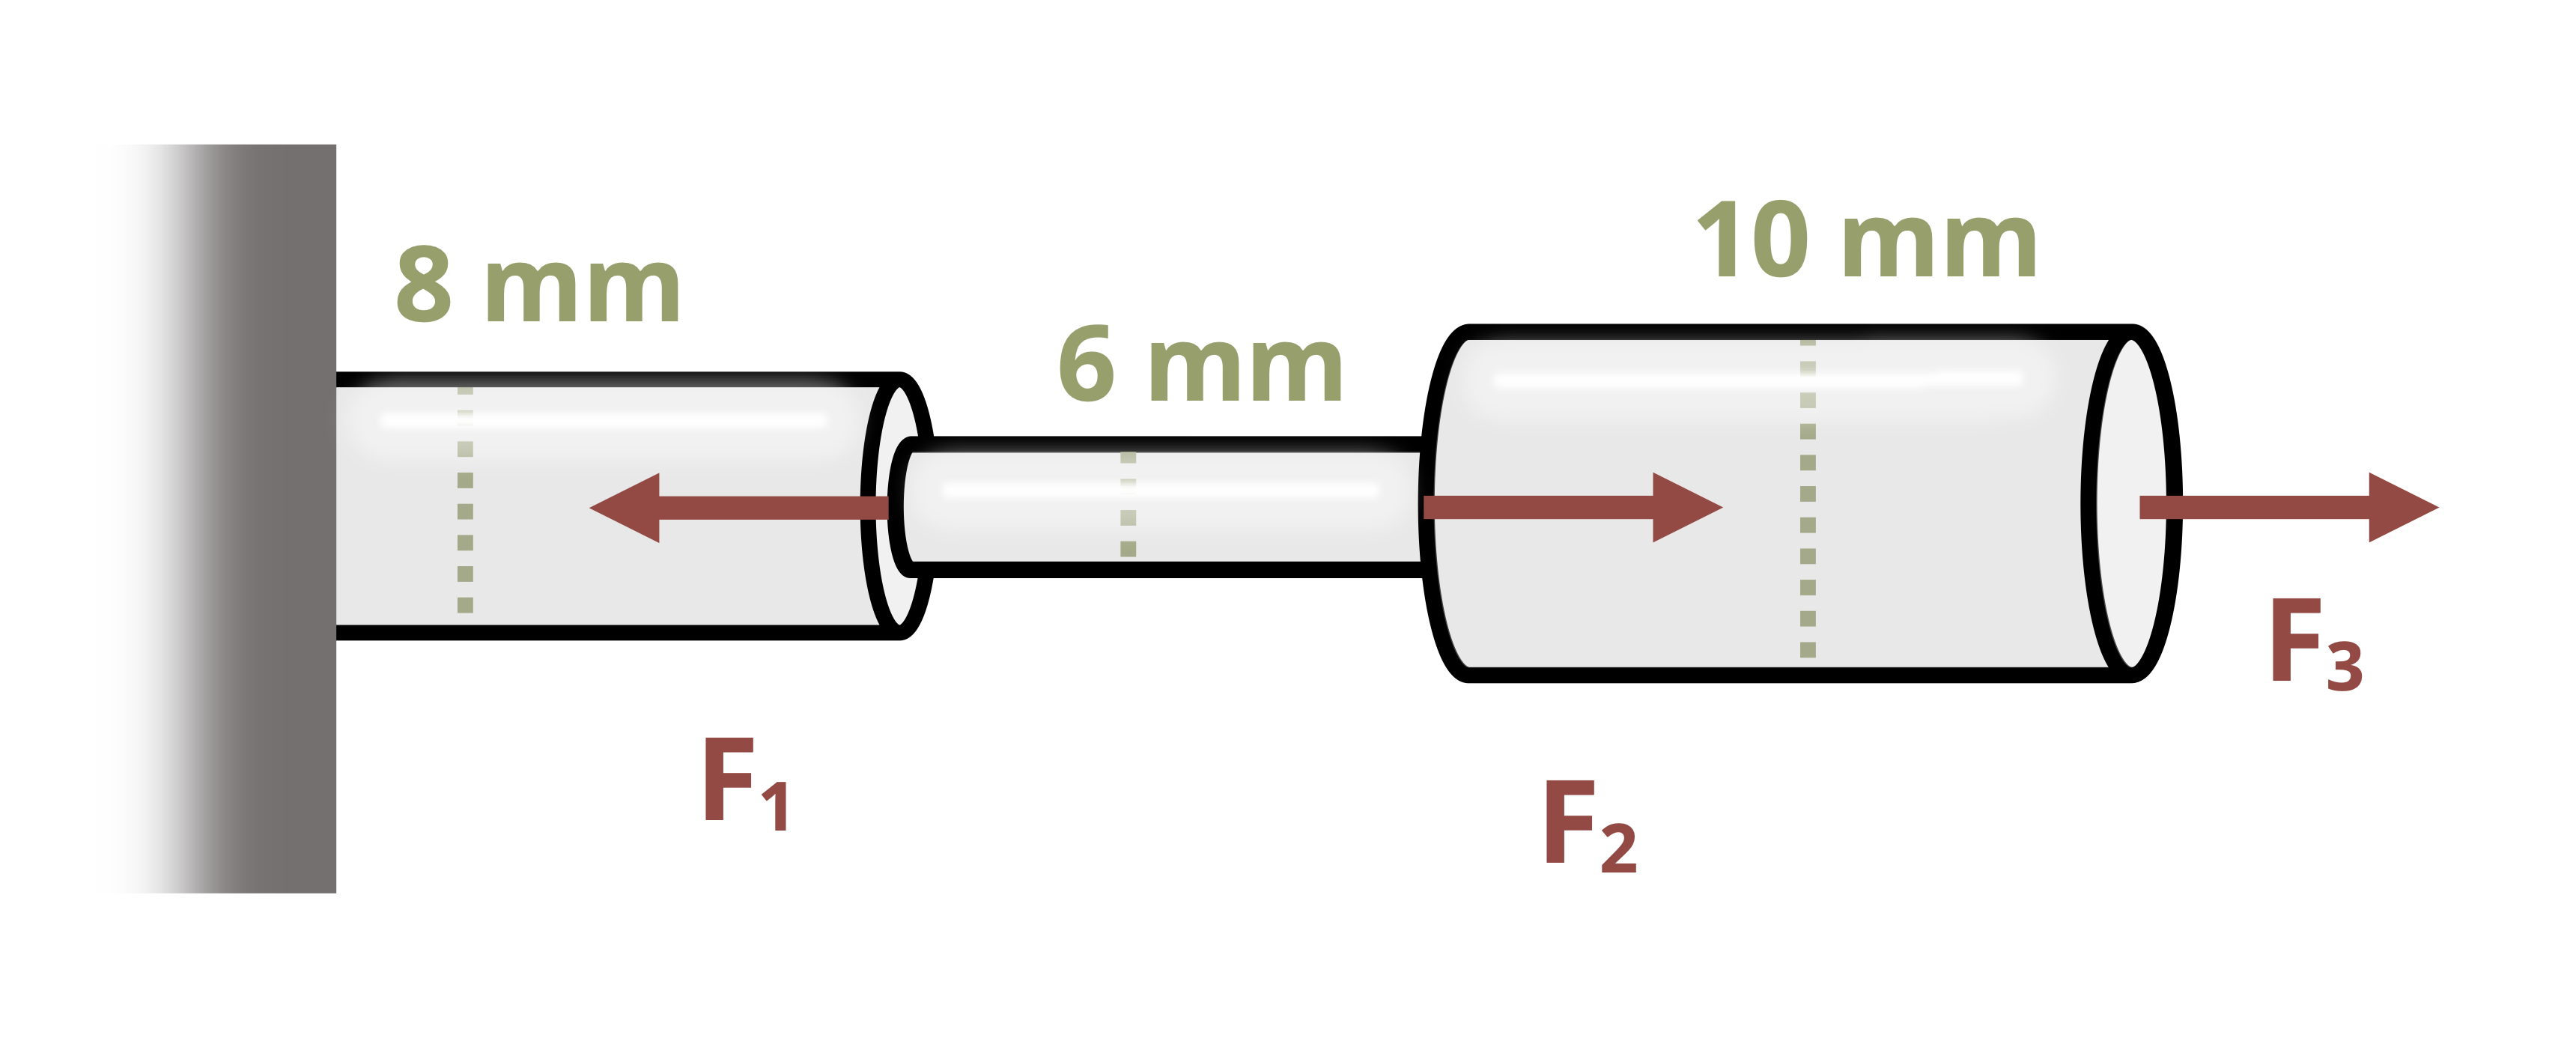
\includegraphics[keepaspectratio]{images/138.png}}

}

\caption{Figure 1: A series of solid circular bars are loaded with three
loads}

\end{figure}%

{[}Problem adapted from © Kurt Gramoll CC BY NC-SA 4.0{]}

\begin{Shaded}
\begin{Highlighting}[]
\NormalTok{\#| standalone: true}
\NormalTok{\#| viewerHeight: 600}
\NormalTok{\#| components: [viewer]}

\NormalTok{from shiny import App, render, ui, reactive}
\NormalTok{import random}
\NormalTok{import asyncio}
\NormalTok{import io}
\NormalTok{import math}
\NormalTok{import string}
\NormalTok{from datetime import datetime}
\NormalTok{from pathlib import Path}


\NormalTok{def generate\_random\_letters(length):}
\NormalTok{    \# Generate a random string of letters of specified length}
\NormalTok{    return \textquotesingle{}\textquotesingle{}.join(random.choice(string.ascii\_lowercase) for \_ in range(length))  }

\NormalTok{problem\_ID="138"}
\NormalTok{F1=reactive.Value("\_\_")}
\NormalTok{F2=reactive.Value("\_\_")}
\NormalTok{F3=reactive.Value("\_\_")}
\NormalTok{d1=8}
\NormalTok{d2=6}
\NormalTok{d3=10}
\NormalTok{attempts=["Timestamp,Attempt,Answer,Feedback\textbackslash{}n"]}

\NormalTok{app\_ui = ui.page\_fluid(}
\NormalTok{    ui.markdown("**Please enter your ID number from your instructor and click to generate your problem**"),}
\NormalTok{    ui.input\_text("ID","", placeholder="Enter ID Number Here"),}
\NormalTok{    ui.input\_action\_button("generate\_problem", "Generate Problem", class\_="btn{-}primary"),}
\NormalTok{    ui.markdown("**Problem Statement**"),}
\NormalTok{    ui.output\_ui("ui\_problem\_statement"),}
\NormalTok{    ui.input\_text("answer","Your Answer in units of MPa", placeholder="Please enter your answer"),}
\NormalTok{    ui.input\_action\_button("submit", "Submit Answer", class\_="btn{-}primary"),}
\NormalTok{    ui.download\_button("download", "Download File to Submit", class\_="btn{-}success"),}
\NormalTok{)}


\NormalTok{def server(input, output, session):}
\NormalTok{    \# Initialize a counter for attempts}
\NormalTok{    attempt\_counter = reactive.Value(0)}
    
\NormalTok{    @output}
\NormalTok{    @render.ui}
\NormalTok{    def ui\_problem\_statement():}
\NormalTok{        return[ui.markdown(f"A series of solid circular bars are loaded with three loads as shown, F\textless{}sub\textgreater{}1\textless{}/sub\textgreater{} = \{F1()\} N, F\textless{}sub\textgreater{}2\textless{}/sub\textgreater{} = \{F2()\} N, and F\textless{}sub\textgreater{}3\textless{}/sub\textgreater{} = \{F3()\} N. What is the largest absolute normal stress, 𝜎, in any bar?")]}
     
\NormalTok{    @reactive.Effect}
\NormalTok{    @reactive.event(input.generate\_problem)}
\NormalTok{    def randomize\_vars():}
\NormalTok{        random.seed(input.ID())}
\NormalTok{        F1.set(random.randrange(50, 70, 1))}
\NormalTok{        F2.set(random.randrange(10, 30, 1))}
\NormalTok{        F3.set(F1(){-}F2())}
        

\NormalTok{    @reactive.Effect}
\NormalTok{    @reactive.event(input.submit)}
\NormalTok{    def \_():}
\NormalTok{        attempt\_counter.set(attempt\_counter() + 1)  \# Increment the attempt counter on each submission.}
        
\NormalTok{        \# Calculate the instructor\textquotesingle{}s answer and determine if the user\textquotesingle{}s answer is correct.}
\NormalTok{        instr= (F1()/(math.pi*(d2/(1000*2))**2))/10**6}
        
\NormalTok{        if math.isclose(float(input.answer()), instr, rel\_tol=0.01):}
\NormalTok{            check = "*Correct*"}
\NormalTok{            correct\_indicator = "JL"}
\NormalTok{        else:}
\NormalTok{            check = "*Not Correct.*"}
\NormalTok{            correct\_indicator = "JG"}

\NormalTok{        \# Generate random parts for the encoded attempt.}
\NormalTok{        random\_start = generate\_random\_letters(4)}
\NormalTok{        random\_middle = generate\_random\_letters(4)}
\NormalTok{        random\_end = generate\_random\_letters(4)}
\NormalTok{        encoded\_attempt = f"\{random\_start\}\{problem\_ID\}{-}\{random\_middle\}\{attempt\_counter()\}\{correct\_indicator\}{-}\{random\_end\}\{input.ID()\}"}

\NormalTok{        \# Store the most recent encoded attempt in a reactive value so it persists across submissions}
\NormalTok{        session.encoded\_attempt = reactive.Value(encoded\_attempt)}

\NormalTok{        \# Append the attempt data to the attempts list without the encoded attempt}
\NormalTok{        attempts.append(f"\{datetime.now()\}, \{attempt\_counter()\}, \{input.answer()\}, \{check\}\textbackslash{}n")}

\NormalTok{        \# Show feedback to the user.}
\NormalTok{        feedback = ui.markdown(f"Your answer of \{input.answer()\} is \{check\}.")}
\NormalTok{        m = ui.modal(}
\NormalTok{            feedback,}
\NormalTok{            title="Feedback",}
\NormalTok{            easy\_close=True}
\NormalTok{        )}
\NormalTok{        ui.modal\_show(m)}

\NormalTok{    @session.download(filename=lambda: f"Problem\_Log{-}\{problem\_ID\}{-}\{input.ID()\}.csv")}
\NormalTok{    async def download():}
\NormalTok{        \# Start the CSV with the encoded attempt (without label)}
\NormalTok{        final\_encoded = session.encoded\_attempt() if session.encoded\_attempt is not None else "No attempts"}
\NormalTok{        yield f"\{final\_encoded\}\textbackslash{}n\textbackslash{}n"}
        
\NormalTok{        \# Write the header for the remaining CSV data once}
\NormalTok{        yield "Timestamp,Attempt,Answer,Feedback\textbackslash{}n"}
        
\NormalTok{        \# Write the attempts data, ensure that the header from the attempts list is not written again}
\NormalTok{        for attempt in attempts[1:]:  \# Skip the first element which is the header}
\NormalTok{            await asyncio.sleep(0.25)  \# This delay may not be necessary; adjust as needed}
\NormalTok{            yield attempt}


\NormalTok{\# App installation}
\NormalTok{app = App(app\_ui, server)}
\end{Highlighting}
\end{Shaded}

\chapter*{Problem 2.2 - Average Normal
Stress}\label{problem-2.2---average-normal-stress}
\addcontentsline{toc}{chapter}{Problem 2.2 - Average Normal Stress}

\markboth{Problem 2.2 - Average Normal Stress}{Problem 2.2 - Average
Normal Stress}

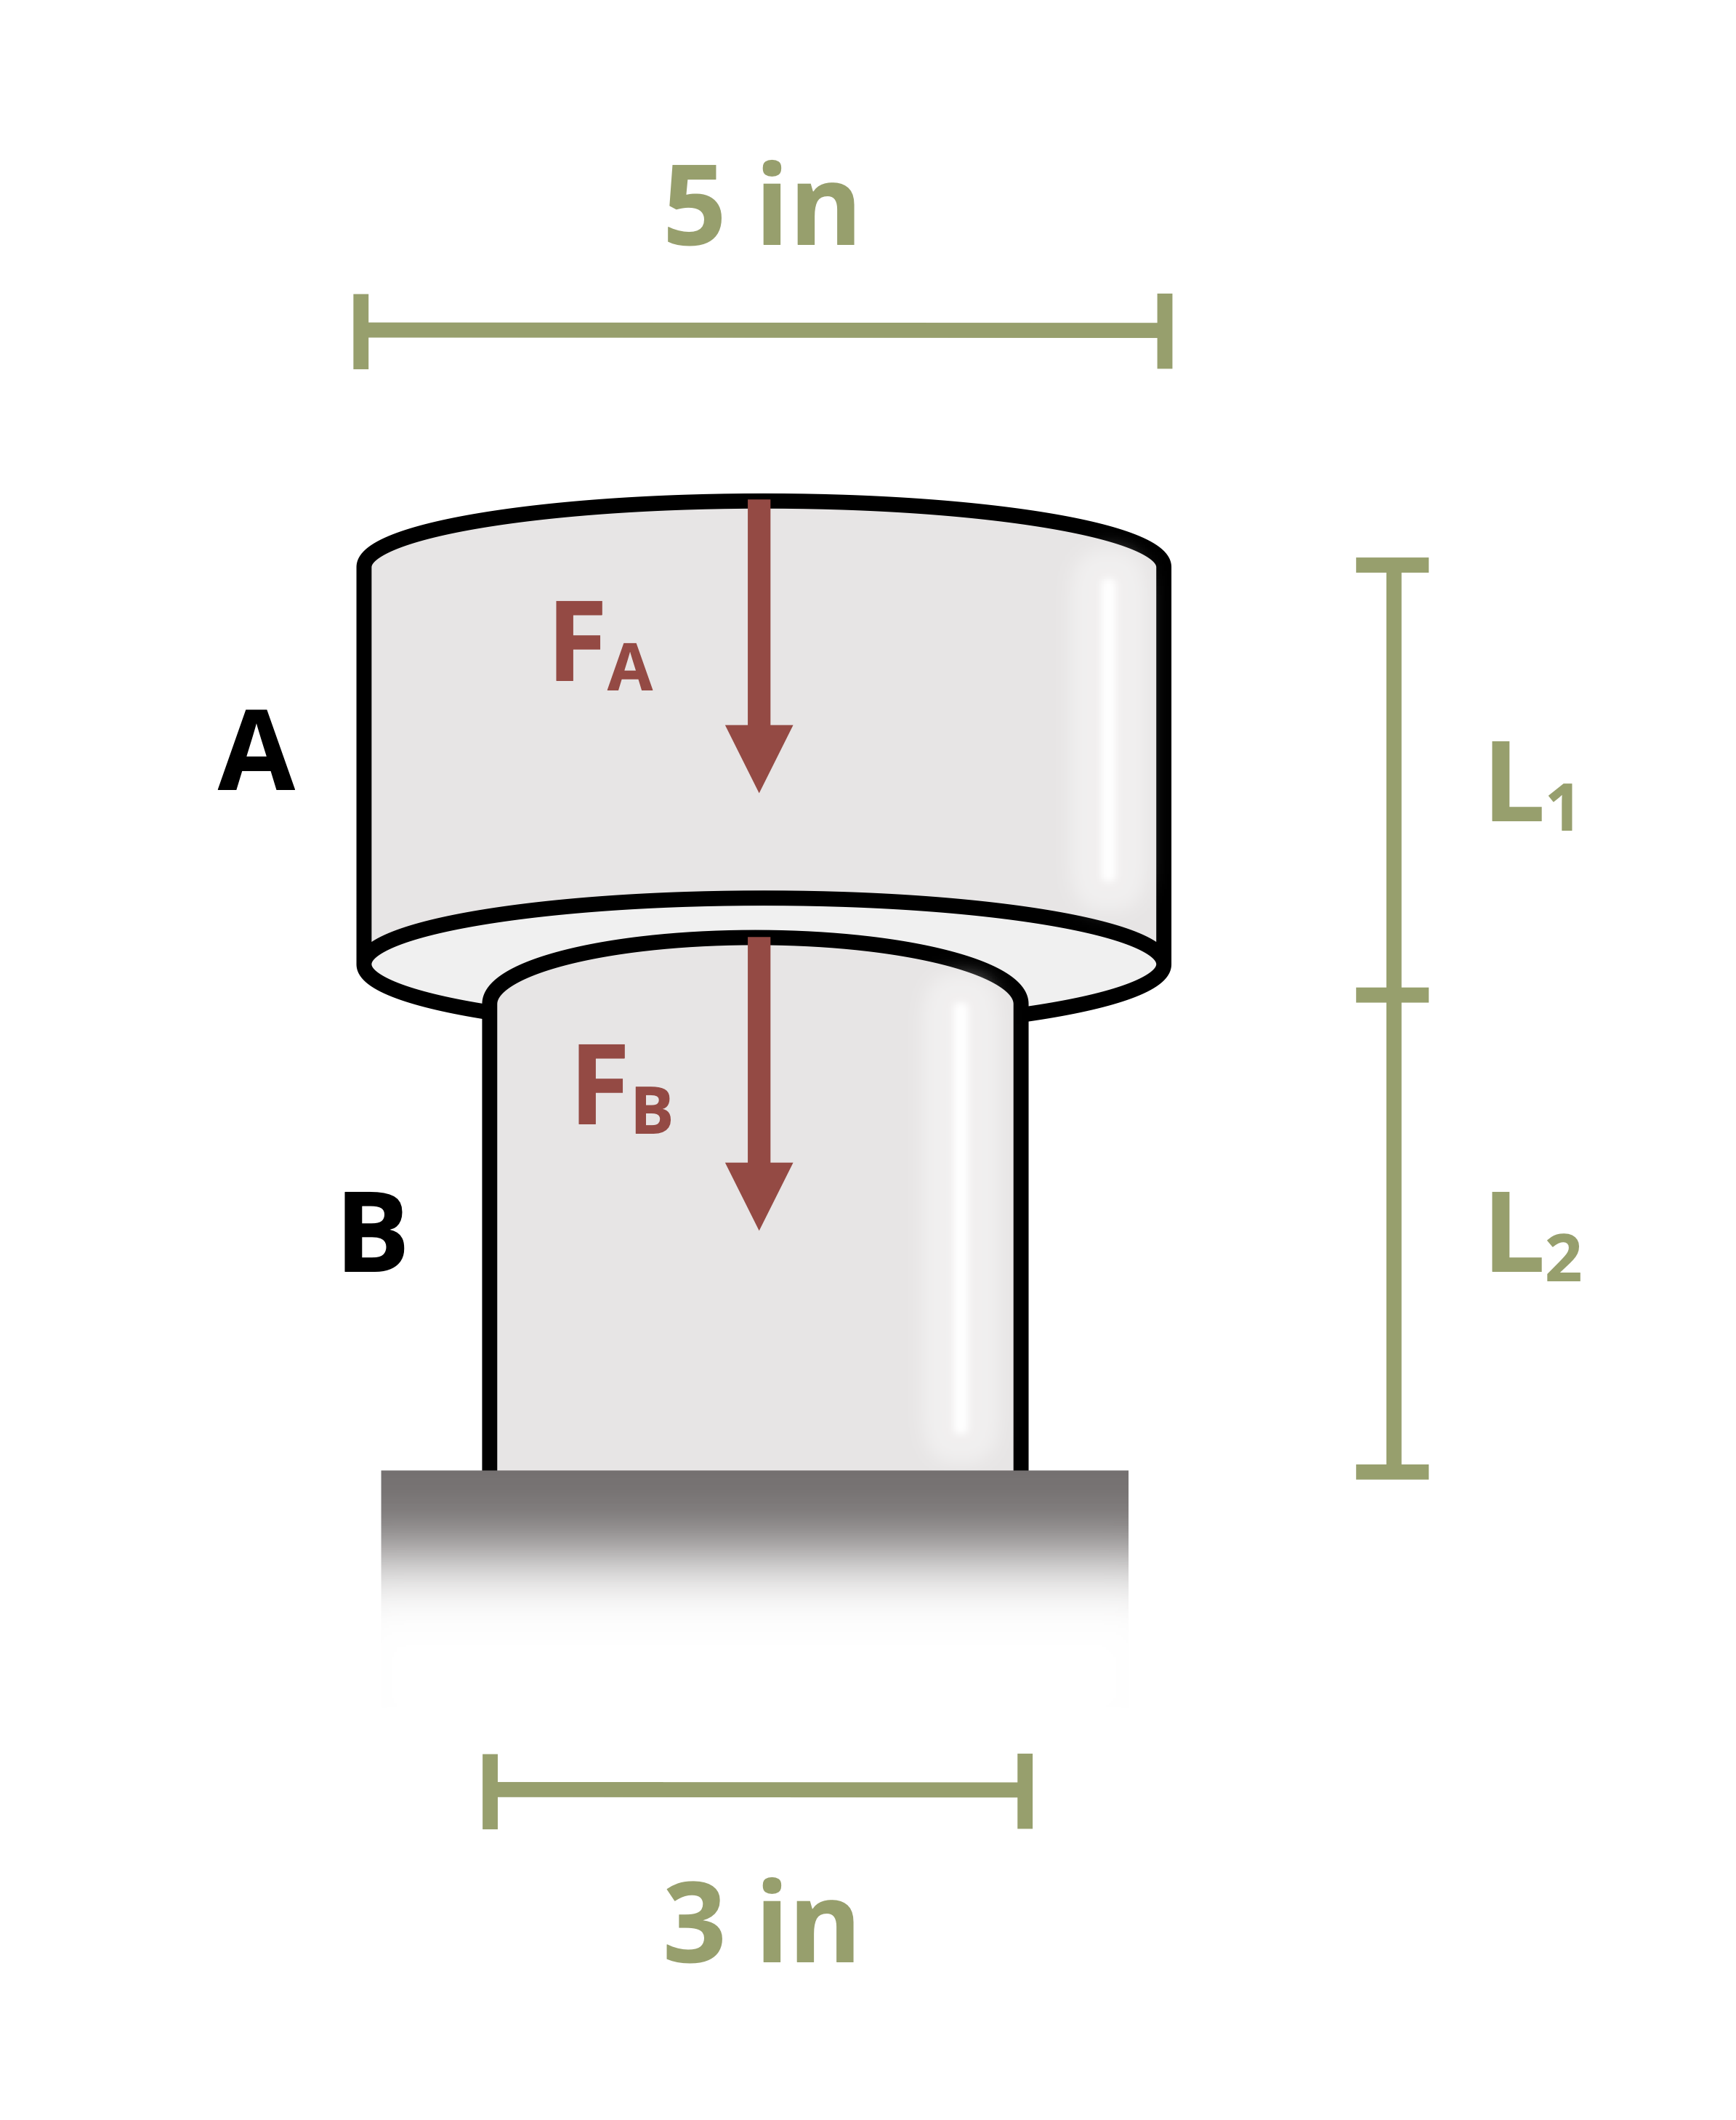
\includegraphics[width=8.52083in,height=\textheight,keepaspectratio]{images/139.png}
{[}Problem adapted from © Kurt Gramoll CC BY NC-SA 4.0{]}

\begin{Shaded}
\begin{Highlighting}[]
\NormalTok{\#| standalone: true}
\NormalTok{\#| viewerHeight: 600}
\NormalTok{\#| components: [viewer]}

\NormalTok{from shiny import App, render, ui, reactive}
\NormalTok{import random}
\NormalTok{import asyncio}
\NormalTok{import io}
\NormalTok{import math}
\NormalTok{import string}
\NormalTok{from datetime import datetime}
\NormalTok{from pathlib import Path}

\NormalTok{def generate\_random\_letters(length):}
\NormalTok{    \# Generate a random string of letters of specified length}
\NormalTok{    return \textquotesingle{}\textquotesingle{}.join(random.choice(string.ascii\_lowercase) for \_ in range(length))  }

\NormalTok{problem\_ID="139"}
\NormalTok{L1=reactive.Value("\_\_")}
\NormalTok{L2=reactive.Value("\_\_")}
\NormalTok{FA=reactive.Value("\_\_")}
\NormalTok{FB=reactive.Value("\_\_")}
\NormalTok{E = 30*10**6}
  
\NormalTok{attempts=["Timestamp,Attempt,Answer,Feedback\textbackslash{}n"]}

\NormalTok{app\_ui = ui.page\_fluid(}
\NormalTok{    ui.markdown("**Please enter your ID number from your instructor and click to generate your problem**"),}
\NormalTok{    ui.input\_text("ID","", placeholder="Enter ID Number Here"),}
\NormalTok{    ui.input\_action\_button("generate\_problem", "Generate Problem", class\_="btn{-}primary"),}
\NormalTok{    ui.markdown("**Problem Statement**"),}
\NormalTok{    ui.output\_ui("ui\_problem\_statement"),}
\NormalTok{    ui.input\_text("answer","Your Answer in units of psi", placeholder="Please enter your answer"),}
\NormalTok{    ui.input\_action\_button("submit", "Submit Answer", class\_="btn{-}primary"),}
\NormalTok{    ui.download\_button("download", "Download File to Submit", class\_="btn{-}success"),}
\NormalTok{)}

\NormalTok{def server(input, output, session):}
\NormalTok{    \# Initialize a counter for attempts}
\NormalTok{    attempt\_counter = reactive.Value(0)}

\NormalTok{    @output}
\NormalTok{    @render.ui}
\NormalTok{    def ui\_problem\_statement():}
\NormalTok{        return[ui.markdown(f"Two cylinders are stacked on top of one another and two forces are applied at the top surface and at the joint between the cylinders as shown. If L\textless{}sub\textgreater{}1\textless{}/sub\textgreater{} = \{L1()\} in., L\textless{}sub\textgreater{}2\textless{}/sub\textgreater{} = \{L2()\} in., F\textless{}sub\textgreater{}A\textless{}/sub\textgreater{} = \{FA()\} lb, and F\textless{}sub\textgreater{}B\textless{}/sub\textgreater{} = \{FB()\} lb, determine the average normal stress in cylinder B. Enter a positive answer for tensile stress or a negative answer for compressive stress. ")]}
    
\NormalTok{    @reactive.Effect}
\NormalTok{    @reactive.event(input.generate\_problem)}
\NormalTok{    def randomize\_vars():}
\NormalTok{        random.seed(input.ID())}
\NormalTok{        FA.set(random.randrange(300, 700, 10))}
\NormalTok{        FB.set(random.randrange(100, 300, 10))}
\NormalTok{        L1.set(random.randrange(2, 7, 1))}
\NormalTok{        L2.set(round(L1() * 1.3,1))}
        
\NormalTok{    @reactive.Effect}
\NormalTok{    @reactive.event(input.submit)}
\NormalTok{    def \_():}
\NormalTok{        attempt\_counter.set(attempt\_counter() + 1)  \# Increment the attempt counter on each submission.}
    
\NormalTok{        instr = {-}(FA()+FB())/(math.pi*1.5**2)}
\NormalTok{        if math.isclose(float(input.answer()), instr, rel\_tol=0.01):}
\NormalTok{            check = "*Correct*"}
\NormalTok{            correct\_indicator = "JL"}
\NormalTok{        else:}
\NormalTok{            check = "*Not Correct.*"}
\NormalTok{            correct\_indicator = "JG"}

\NormalTok{        \# Generate random parts for the encoded attempt.}
\NormalTok{        random\_start = generate\_random\_letters(4)}
\NormalTok{        random\_middle = generate\_random\_letters(4)}
\NormalTok{        random\_end = generate\_random\_letters(4)}
\NormalTok{        encoded\_attempt = f"\{random\_start\}\{problem\_ID\}{-}\{random\_middle\}\{attempt\_counter()\}\{correct\_indicator\}{-}\{random\_end\}\{input.ID()\}"}

\NormalTok{        \# Store the most recent encoded attempt in a reactive value so it persists across submissions}
\NormalTok{        session.encoded\_attempt = reactive.Value(encoded\_attempt)}

\NormalTok{        \# Append the attempt data to the attempts list without the encoded attempt}
\NormalTok{        attempts.append(f"\{datetime.now()\}, \{attempt\_counter()\}, \{input.answer()\}, \{check\}\textbackslash{}n")}

\NormalTok{        \# Show feedback to the user.}
\NormalTok{        feedback = ui.markdown(f"Your answer of \{input.answer()\} is \{check\}.")}
\NormalTok{        m = ui.modal(}
\NormalTok{            feedback,}
\NormalTok{            title="Feedback",}
\NormalTok{            easy\_close=True}
\NormalTok{        )}
\NormalTok{        ui.modal\_show(m)}

\NormalTok{    @session.download(filename=lambda: f"Problem\_Log{-}\{problem\_ID\}{-}\{input.ID()\}.csv")}
\NormalTok{    async def download():}
\NormalTok{        \# Start the CSV with the encoded attempt (without label)}
\NormalTok{        final\_encoded = session.encoded\_attempt() if session.encoded\_attempt is not None else "No attempts"}
\NormalTok{        yield f"\{final\_encoded\}\textbackslash{}n\textbackslash{}n"}
        
\NormalTok{        \# Write the header for the remaining CSV data once}
\NormalTok{        yield "Timestamp,Attempt,Answer,Feedback\textbackslash{}n"}
        
\NormalTok{        \# Write the attempts data, ensure that the header from the attempts list is not written again}
\NormalTok{        for attempt in attempts[1:]:  \# Skip the first element which is the header}
\NormalTok{            await asyncio.sleep(0.25)  \# This delay may not be necessary; adjust as needed}
\NormalTok{            yield attempt}

\NormalTok{\# App installation}
\NormalTok{app = App(app\_ui, server)}
\end{Highlighting}
\end{Shaded}

\chapter*{Problem 2.3 - Average Normal
Stress}\label{problem-2.3---average-normal-stress}
\addcontentsline{toc}{chapter}{Problem 2.3 - Average Normal Stress}

\markboth{Problem 2.3 - Average Normal Stress}{Problem 2.3 - Average
Normal Stress}

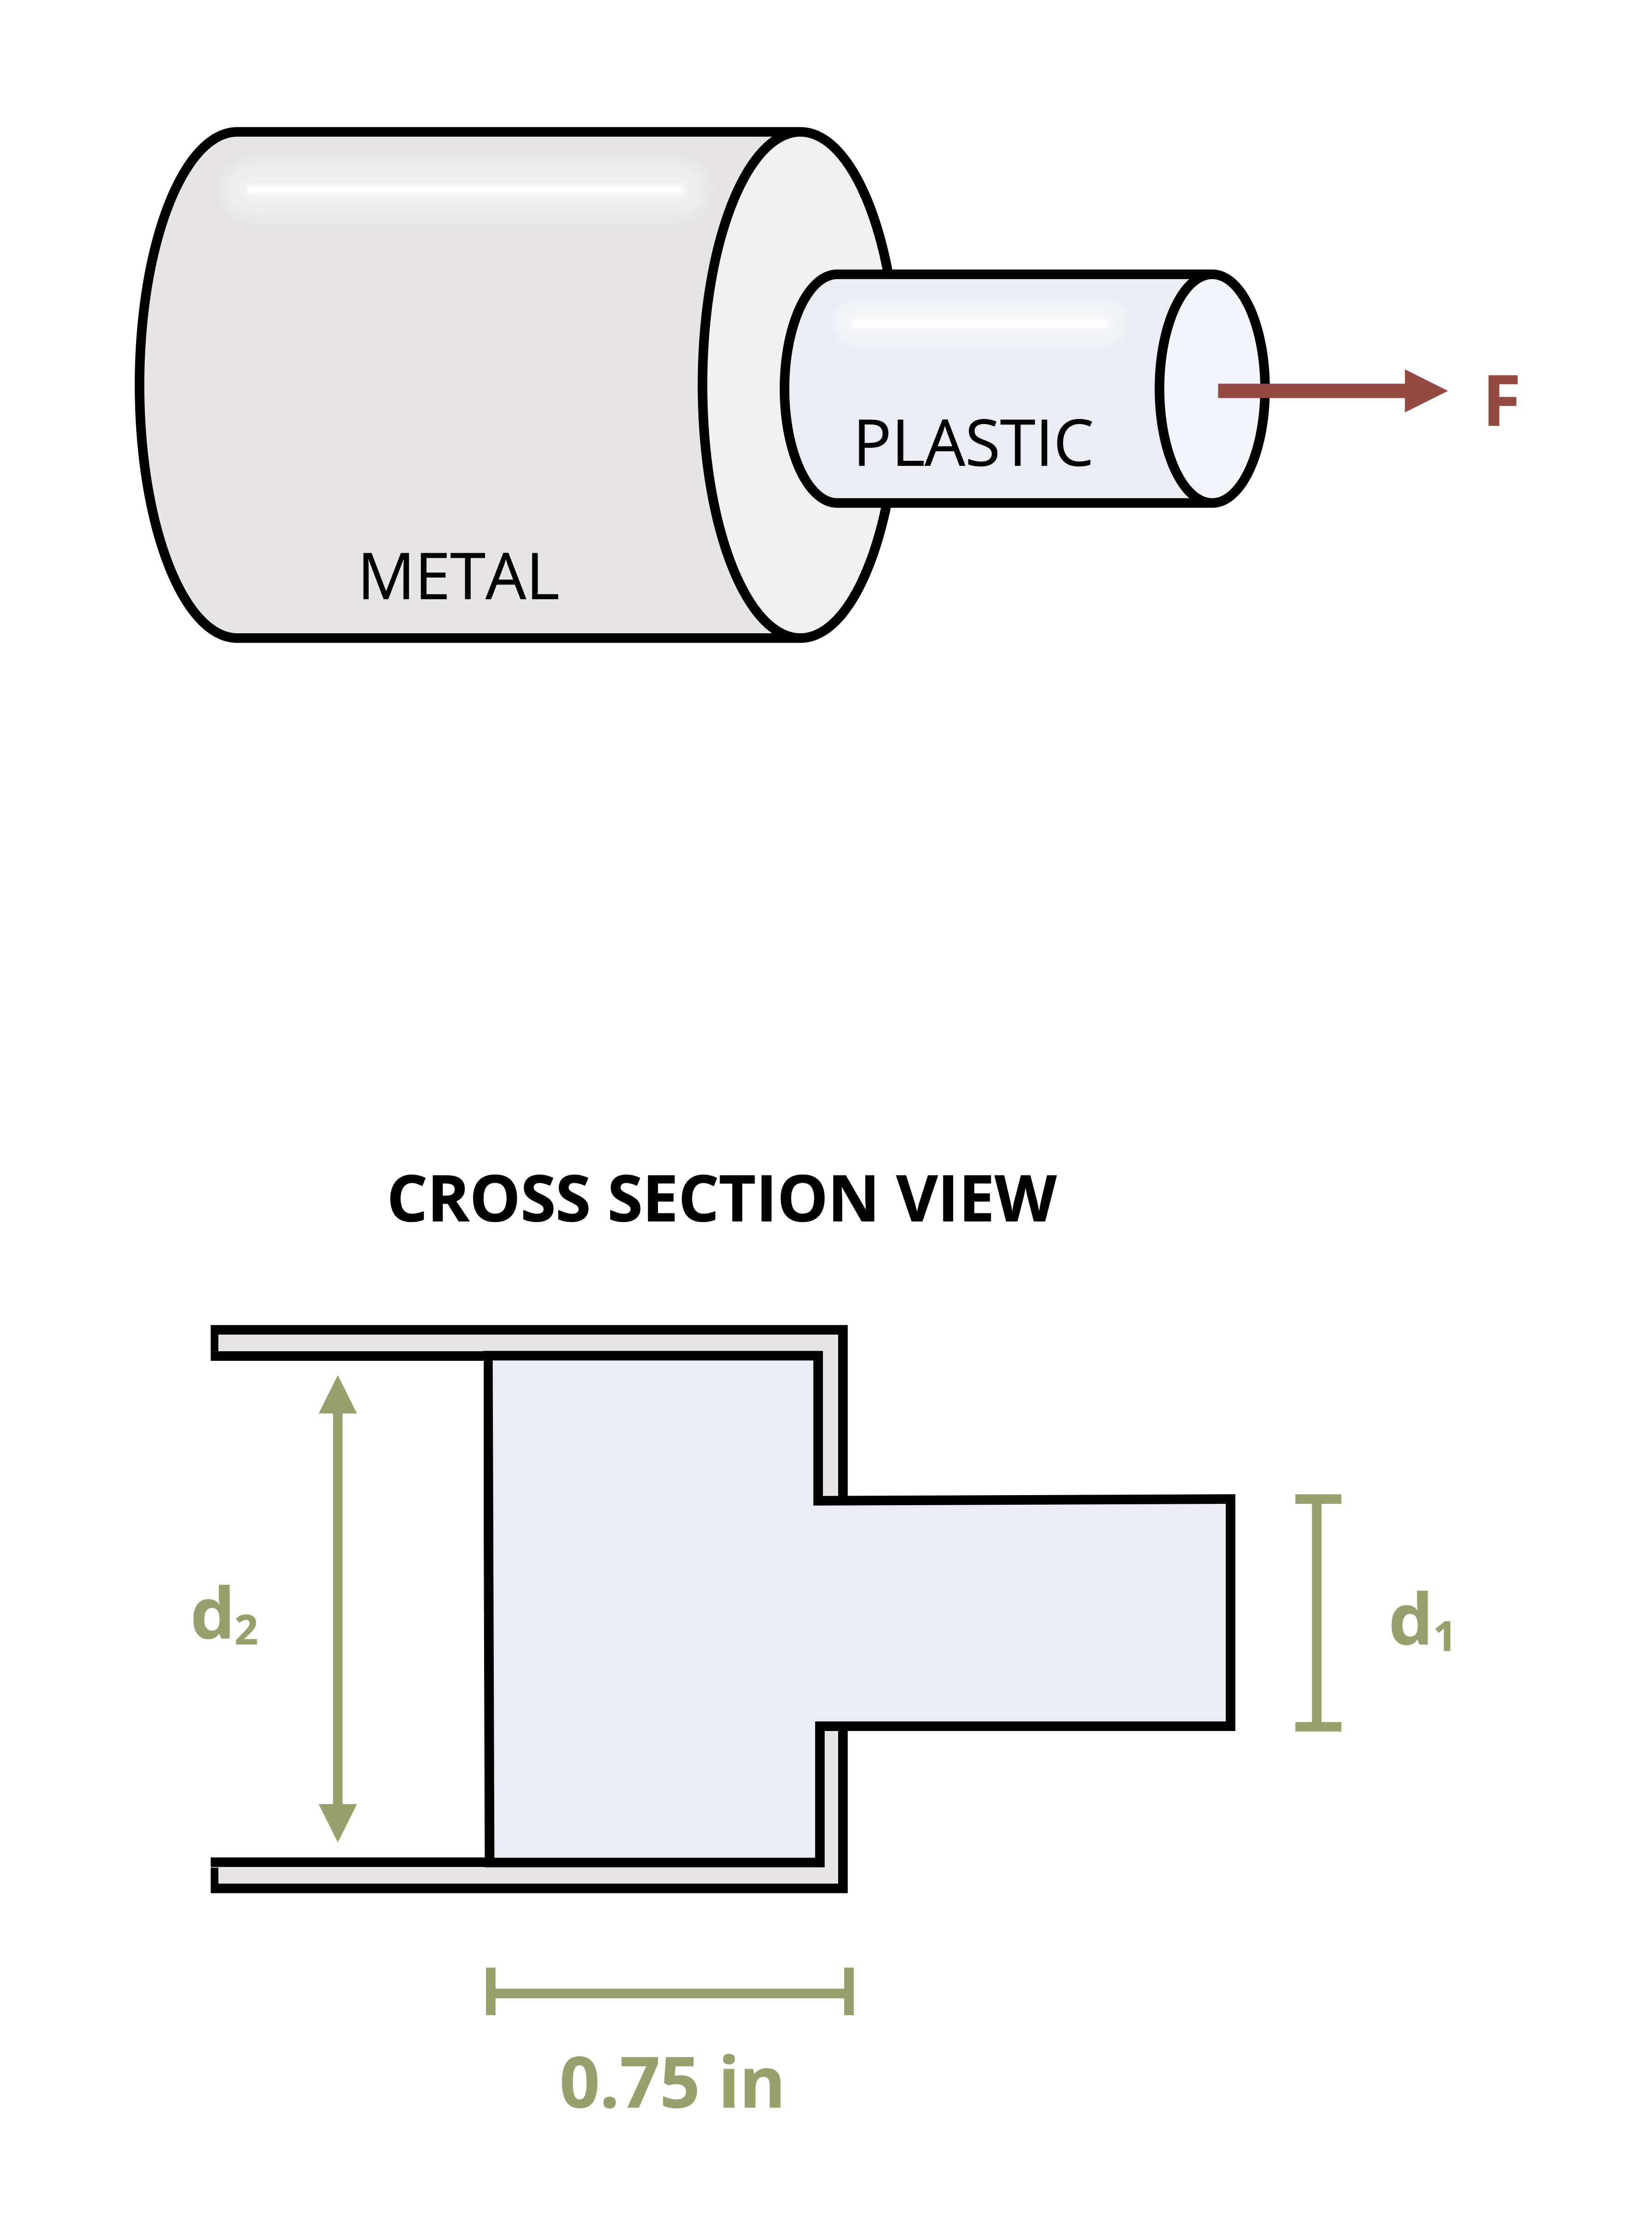
\includegraphics[width=9.33333in,height=\textheight,keepaspectratio]{images/144.png}
{[}Problem adapted from © Kurt Gramoll CC BY NC-SA 4.0{]}

\begin{Shaded}
\begin{Highlighting}[]
\NormalTok{\#| standalone: true}
\NormalTok{\#| viewerHeight: 600}
\NormalTok{\#| components: [viewer]}

\NormalTok{from shiny import App, render, ui, reactive}
\NormalTok{import random}
\NormalTok{import asyncio}
\NormalTok{import io}
\NormalTok{import math}
\NormalTok{import string}
\NormalTok{from datetime import datetime}
\NormalTok{from pathlib import Path}

\NormalTok{def generate\_random\_letters(length):}
\NormalTok{    \# Generate a random string of letters of specified length}
\NormalTok{    return \textquotesingle{}\textquotesingle{}.join(random.choice(string.ascii\_lowercase) for \_ in range(length))}

\NormalTok{problem\_ID="144"}
\NormalTok{F=reactive.Value("\_\_")}
\NormalTok{d1=reactive.Value("\_\_")}
\NormalTok{d2=reactive.Value("\_\_")}

\NormalTok{attempts=["Timestamp,Attempt,Answer,Feedback\textbackslash{}n"]}

\NormalTok{app\_ui = ui.page\_fluid(}
\NormalTok{    ui.markdown("**Please enter your ID number from your instructor and click to generate your problem**"),}
\NormalTok{    ui.input\_text("ID","", placeholder="Enter ID Number Here"),}
\NormalTok{    ui.input\_action\_button("generate\_problem", "Generate Problem", class\_="btn{-}primary"),}
\NormalTok{    ui.markdown("**Problem Statement**"),}
\NormalTok{    ui.output\_ui("ui\_problem\_statement"),}
\NormalTok{    ui.input\_text("answer","Your Answer in units of psi", placeholder="Please enter your answer"),}
\NormalTok{    ui.input\_action\_button("submit", "Submit Answer", class\_="btn{-}primary"),}
\NormalTok{    ui.download\_button("download", "Download File to Submit", class\_="btn{-}success"),}
\NormalTok{)}


\NormalTok{def server(input, output, session):}
\NormalTok{    \# Initialize a counter for attempts}
\NormalTok{    attempt\_counter = reactive.Value(0)}

\NormalTok{    @output}
\NormalTok{    @render.ui}
\NormalTok{    def ui\_problem\_statement():}
\NormalTok{        return[ui.markdown(f"A plastic cylindrical peg is constrained by a metal cap as shown. An axial load of F = \{F()\} lb is applied to the peg. If d\textless{}sub\textgreater{}1\textless{}/sub\textgreater{} = \{d1()\} in and d\textless{}sub\textgreater{}2\textless{}/sub\textgreater{} = \{d2()\} in, determine the largest normal stress in the peg. Assume the axial load is evenly distributed across the peg and that the metal cap is fixed and does not move.")]}
    
\NormalTok{    @reactive.Effect}
\NormalTok{    @reactive.event(input.generate\_problem)}
\NormalTok{    def randomize\_vars():}
\NormalTok{        random.seed(input.ID())}
\NormalTok{        F.set(random.randrange(20, 80, 5))}
\NormalTok{        d1.set(random.randrange(3, 8, 1)/10)}
\NormalTok{        d2.set(round(d1() * 1.6, 2))}
        
 
\NormalTok{    @reactive.Effect}
\NormalTok{    @reactive.event(input.submit)}
\NormalTok{    def \_():}
\NormalTok{        attempt\_counter.set(attempt\_counter() + 1)  \# Increment the attempt counter on each submission.}
\NormalTok{        instr= F()/(math.pi*((d1()/2)**2))}
\NormalTok{        \#check=math.isclose(float(input.answer()),instr,rel\_tol=0.001)}
        
\NormalTok{        if math.isclose(float(input.answer()), instr, rel\_tol=0.01):}
\NormalTok{            check = "*Correct*"}
\NormalTok{            correct\_indicator = "JL"}
\NormalTok{        else:}
\NormalTok{            check = "*Not Correct.*"}
\NormalTok{            correct\_indicator = "JG"}

\NormalTok{        \# Generate random parts for the encoded attempt.}
\NormalTok{        random\_start = generate\_random\_letters(4)}
\NormalTok{        random\_middle = generate\_random\_letters(4)}
\NormalTok{        random\_end = generate\_random\_letters(4)}
\NormalTok{        encoded\_attempt = f"\{random\_start\}\{problem\_ID\}{-}\{random\_middle\}\{attempt\_counter()\}\{correct\_indicator\}{-}\{random\_end\}\{input.ID()\}"}

\NormalTok{        \# Store the most recent encoded attempt in a reactive value so it persists across submissions}
\NormalTok{        session.encoded\_attempt = reactive.Value(encoded\_attempt)}

\NormalTok{        \# Append the attempt data to the attempts list without the encoded attempt}
\NormalTok{        attempts.append(f"\{datetime.now()\}, \{attempt\_counter()\}, \{input.answer()\}, \{check\}\textbackslash{}n")}

\NormalTok{        \# Show feedback to the user.}
\NormalTok{        feedback = ui.markdown(f"Your answer of \{input.answer()\} is \{check\}.")}
\NormalTok{        m = ui.modal(}
\NormalTok{            feedback,}
\NormalTok{            title="Feedback",}
\NormalTok{            easy\_close=True}
\NormalTok{        )}
\NormalTok{        ui.modal\_show(m)}

\NormalTok{    @session.download(filename=lambda: f"Problem\_Log{-}\{problem\_ID\}{-}\{input.ID()\}.csv")}
\NormalTok{    async def download():}
\NormalTok{        \# Start the CSV with the encoded attempt (without label)}
\NormalTok{        final\_encoded = session.encoded\_attempt() if session.encoded\_attempt is not None else "No attempts"}
\NormalTok{        yield f"\{final\_encoded\}\textbackslash{}n\textbackslash{}n"}
        
\NormalTok{        \# Write the header for the remaining CSV data once}
\NormalTok{        yield "Timestamp,Attempt,Answer,Feedback\textbackslash{}n"}
        
\NormalTok{        \# Write the attempts data, ensure that the header from the attempts list is not written again}
\NormalTok{        for attempt in attempts[1:]:  \# Skip the first element which is the header}
\NormalTok{            await asyncio.sleep(0.25)  \# This delay may not be necessary; adjust as needed}
\NormalTok{            yield attempt}


\NormalTok{\# App installation}
\NormalTok{app = App(app\_ui, server)}
\end{Highlighting}
\end{Shaded}

\chapter*{Problem 2.4 - Average Normal
Stress}\label{problem-2.4---average-normal-stress}
\addcontentsline{toc}{chapter}{Problem 2.4 - Average Normal Stress}

\markboth{Problem 2.4 - Average Normal Stress}{Problem 2.4 - Average
Normal Stress}

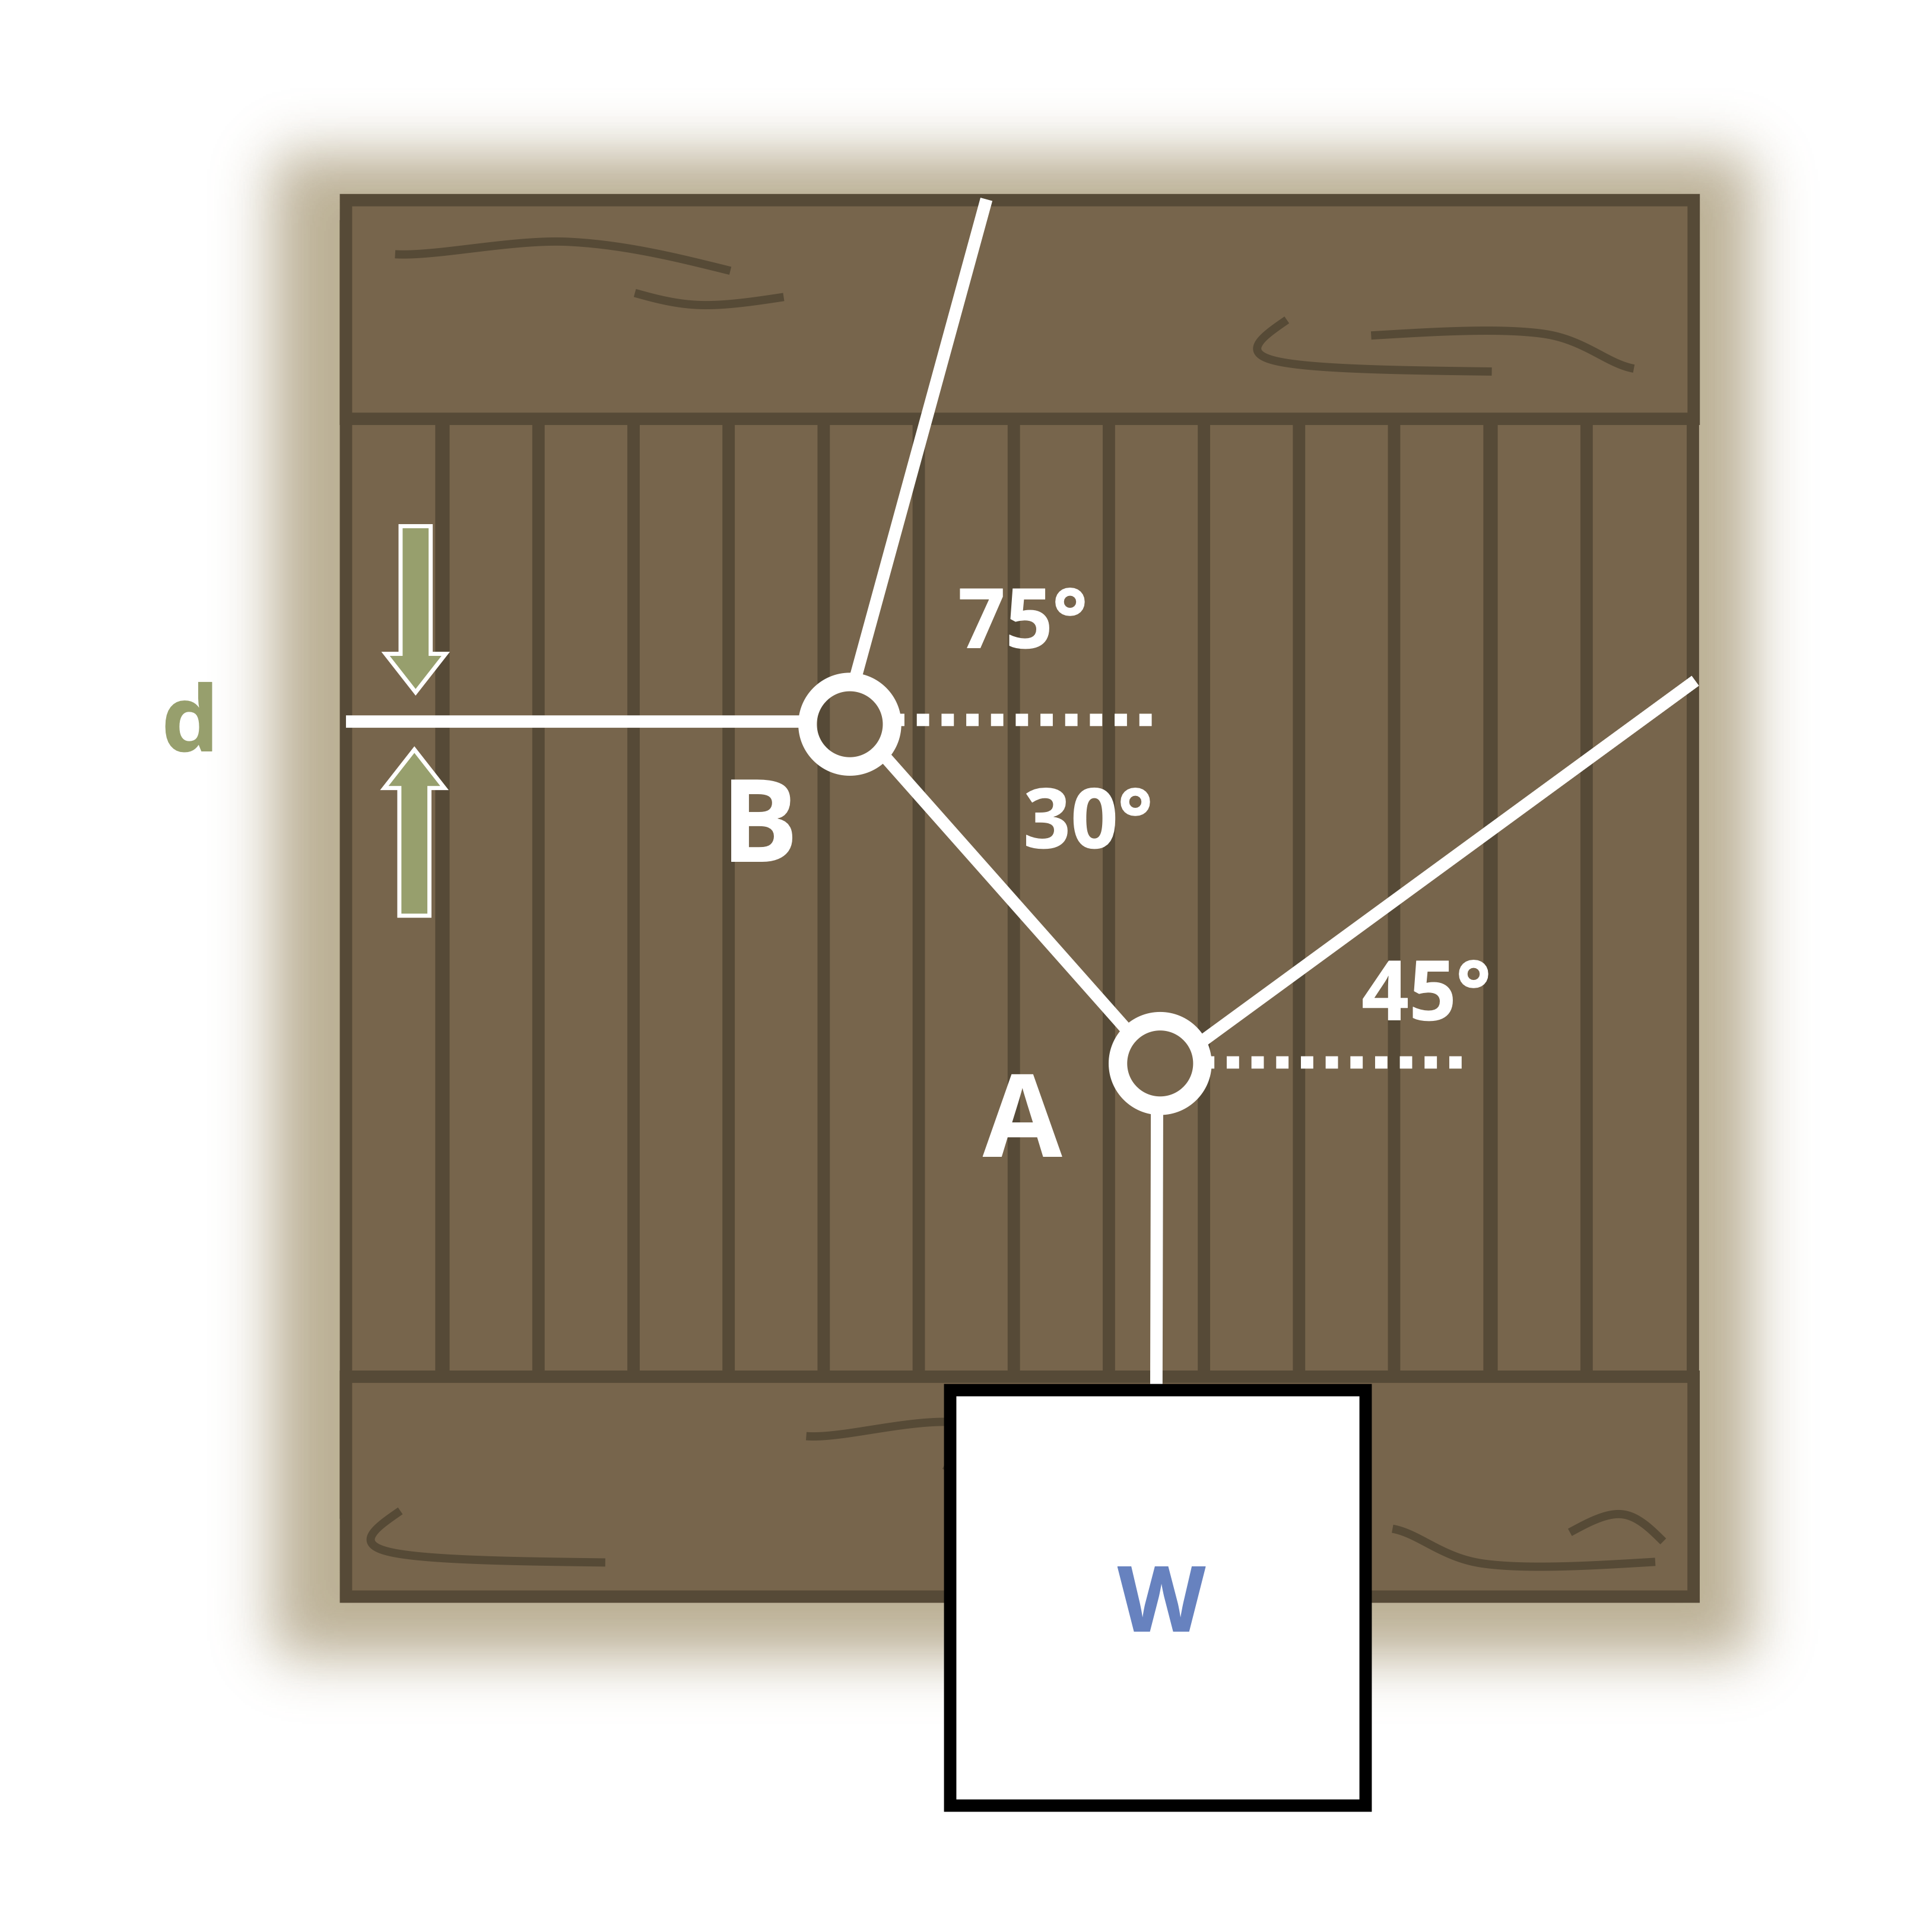
\includegraphics[width=15.48958in,height=\textheight,keepaspectratio]{images/146.png}
{[}Problem adapted from © Kurt Gramoll CC BY NC-SA 4.0{]}

\begin{Shaded}
\begin{Highlighting}[]
\NormalTok{\#| standalone: true}
\NormalTok{\#| viewerHeight: 600}
\NormalTok{\#| components: [viewer]}

\NormalTok{from shiny import App, render, ui, reactive}
\NormalTok{import random}
\NormalTok{import asyncio}
\NormalTok{import io}
\NormalTok{import math}
\NormalTok{import string}
\NormalTok{from datetime import datetime}
\NormalTok{from pathlib import Path}


\NormalTok{def generate\_random\_letters(length):}
\NormalTok{    \# Generate a random string of letters of specified length}
\NormalTok{    return \textquotesingle{}\textquotesingle{}.join(random.choice(string.ascii\_lowercase) for \_ in range(length)) }

\NormalTok{problem\_ID="146"}
\NormalTok{W=reactive.Value("\_\_")}
\NormalTok{d=reactive.Value("\_\_")}
\NormalTok{angle1=math.radians(45)}
\NormalTok{angle2=math.radians(30)}
\NormalTok{angle3=math.radians(75)}

\NormalTok{attempts=["Timestamp,Attempt,Answer,Feedback\textbackslash{}n"]}

\NormalTok{app\_ui = ui.page\_fluid(}
\NormalTok{    ui.markdown("**Please enter your ID number from your instructor and click to generate your problem**"),}
\NormalTok{    ui.input\_text("ID","", placeholder="Enter ID Number Here"),}
\NormalTok{    ui.input\_action\_button("generate\_problem", "Generate Problem", class\_="btn{-}primary"),}
\NormalTok{    ui.markdown("**Problem Statement**"),}
\NormalTok{    ui.output\_ui("ui\_problem\_statement"),}
\NormalTok{    ui.input\_text("answer","Your Answer in units of MPa", placeholder="Please enter your answer"),}
\NormalTok{    ui.input\_action\_button("submit", "Submit Answer", class\_="btn{-}primary"),}
\NormalTok{    ui.download\_button("download", "Download File to Submit", class\_="btn{-}success"),}
\NormalTok{)}


\NormalTok{def server(input, output, session):}
\NormalTok{    \# Initialize a counter for attempts}
\NormalTok{    attempt\_counter = reactive.Value(0)}

\NormalTok{    @output}
\NormalTok{    @render.ui}
\NormalTok{    def ui\_problem\_statement():}
\NormalTok{        return[ui.markdown(f"A crate weighing \{W()\} kN is suspended by a set of cables. The diameter of each cable is \{d()\}  mm. What is the maximum stress in any cable, that is the highest average normal stress, excluding the cable attached to the crate.")]}
    
\NormalTok{    @reactive.Effect}
\NormalTok{    @reactive.event(input.generate\_problem)}
\NormalTok{    def randomize\_vars():}
\NormalTok{        random.seed(input.ID())}
\NormalTok{        W.set(random.randrange(30, 90, 1))}
\NormalTok{        d.set(random.randrange(20, 60, 1))}
        

\NormalTok{    @reactive.Effect}
\NormalTok{    @reactive.event(input.submit)}
\NormalTok{    def \_():}
\NormalTok{        attempt\_counter.set(attempt\_counter() + 1)  \# Increment the attempt counter on each submission.}
    
\NormalTok{        R1 = W()/(((math.cos(angle1)/math.cos(angle2))*math.sin(angle2))+math.sin(angle1))}
\NormalTok{        instr = (R1*10**3/(math.pi*((d()/(1000*2))**2)))/10**6}
\NormalTok{        if math.isclose(float(input.answer()), instr, rel\_tol=0.01):}
\NormalTok{            check = "*Correct*"}
\NormalTok{            correct\_indicator = "JL"}
\NormalTok{        else:}
\NormalTok{            check = "*Not Correct.*"}
\NormalTok{            correct\_indicator = "JG"}

\NormalTok{        \# Generate random parts for the encoded attempt.}
\NormalTok{        random\_start = generate\_random\_letters(4)}
\NormalTok{        random\_middle = generate\_random\_letters(4)}
\NormalTok{        random\_end = generate\_random\_letters(4)}
\NormalTok{        encoded\_attempt = f"\{random\_start\}\{problem\_ID\}{-}\{random\_middle\}\{attempt\_counter()\}\{correct\_indicator\}{-}\{random\_end\}\{input.ID()\}"}

\NormalTok{        \# Store the most recent encoded attempt in a reactive value so it persists across submissions}
\NormalTok{        session.encoded\_attempt = reactive.Value(encoded\_attempt)}

\NormalTok{        \# Append the attempt data to the attempts list without the encoded attempt}
\NormalTok{        attempts.append(f"\{datetime.now()\}, \{attempt\_counter()\}, \{input.answer()\}, \{check\}\textbackslash{}n")}

\NormalTok{        \# Show feedback to the user.}
\NormalTok{        feedback = ui.markdown(f"Your answer of \{input.answer()\} is \{check\}.")}
\NormalTok{        m = ui.modal(}
\NormalTok{            feedback,}
\NormalTok{            title="Feedback",}
\NormalTok{            easy\_close=True}
\NormalTok{        )}
\NormalTok{        ui.modal\_show(m)}

\NormalTok{    @session.download(filename=lambda: f"Problem\_Log{-}\{problem\_ID\}{-}\{input.ID()\}.csv")}
\NormalTok{    async def download():}
\NormalTok{        \# Start the CSV with the encoded attempt (without label)}
\NormalTok{        final\_encoded = session.encoded\_attempt() if session.encoded\_attempt is not None else "No attempts"}
\NormalTok{        yield f"\{final\_encoded\}\textbackslash{}n\textbackslash{}n"}
        
\NormalTok{        \# Write the header for the remaining CSV data once}
\NormalTok{        yield "Timestamp,Attempt,Answer,Feedback\textbackslash{}n"}
        
\NormalTok{        \# Write the attempts data, ensure that the header from the attempts list is not written again}
\NormalTok{        for attempt in attempts[1:]:  \# Skip the first element which is the header}
\NormalTok{            await asyncio.sleep(0.25)  \# This delay may not be necessary; adjust as needed}
\NormalTok{            yield attempt}


\NormalTok{\# App installation}
\NormalTok{app = App(app\_ui, server)}
\end{Highlighting}
\end{Shaded}

\chapter*{Problem 2.21 - Average Shear
Stress}\label{problem-2.21---average-shear-stress}
\addcontentsline{toc}{chapter}{Problem 2.21 - Average Shear Stress}

\markboth{Problem 2.21 - Average Shear Stress}{Problem 2.21 - Average
Shear Stress}

\pandocbounded{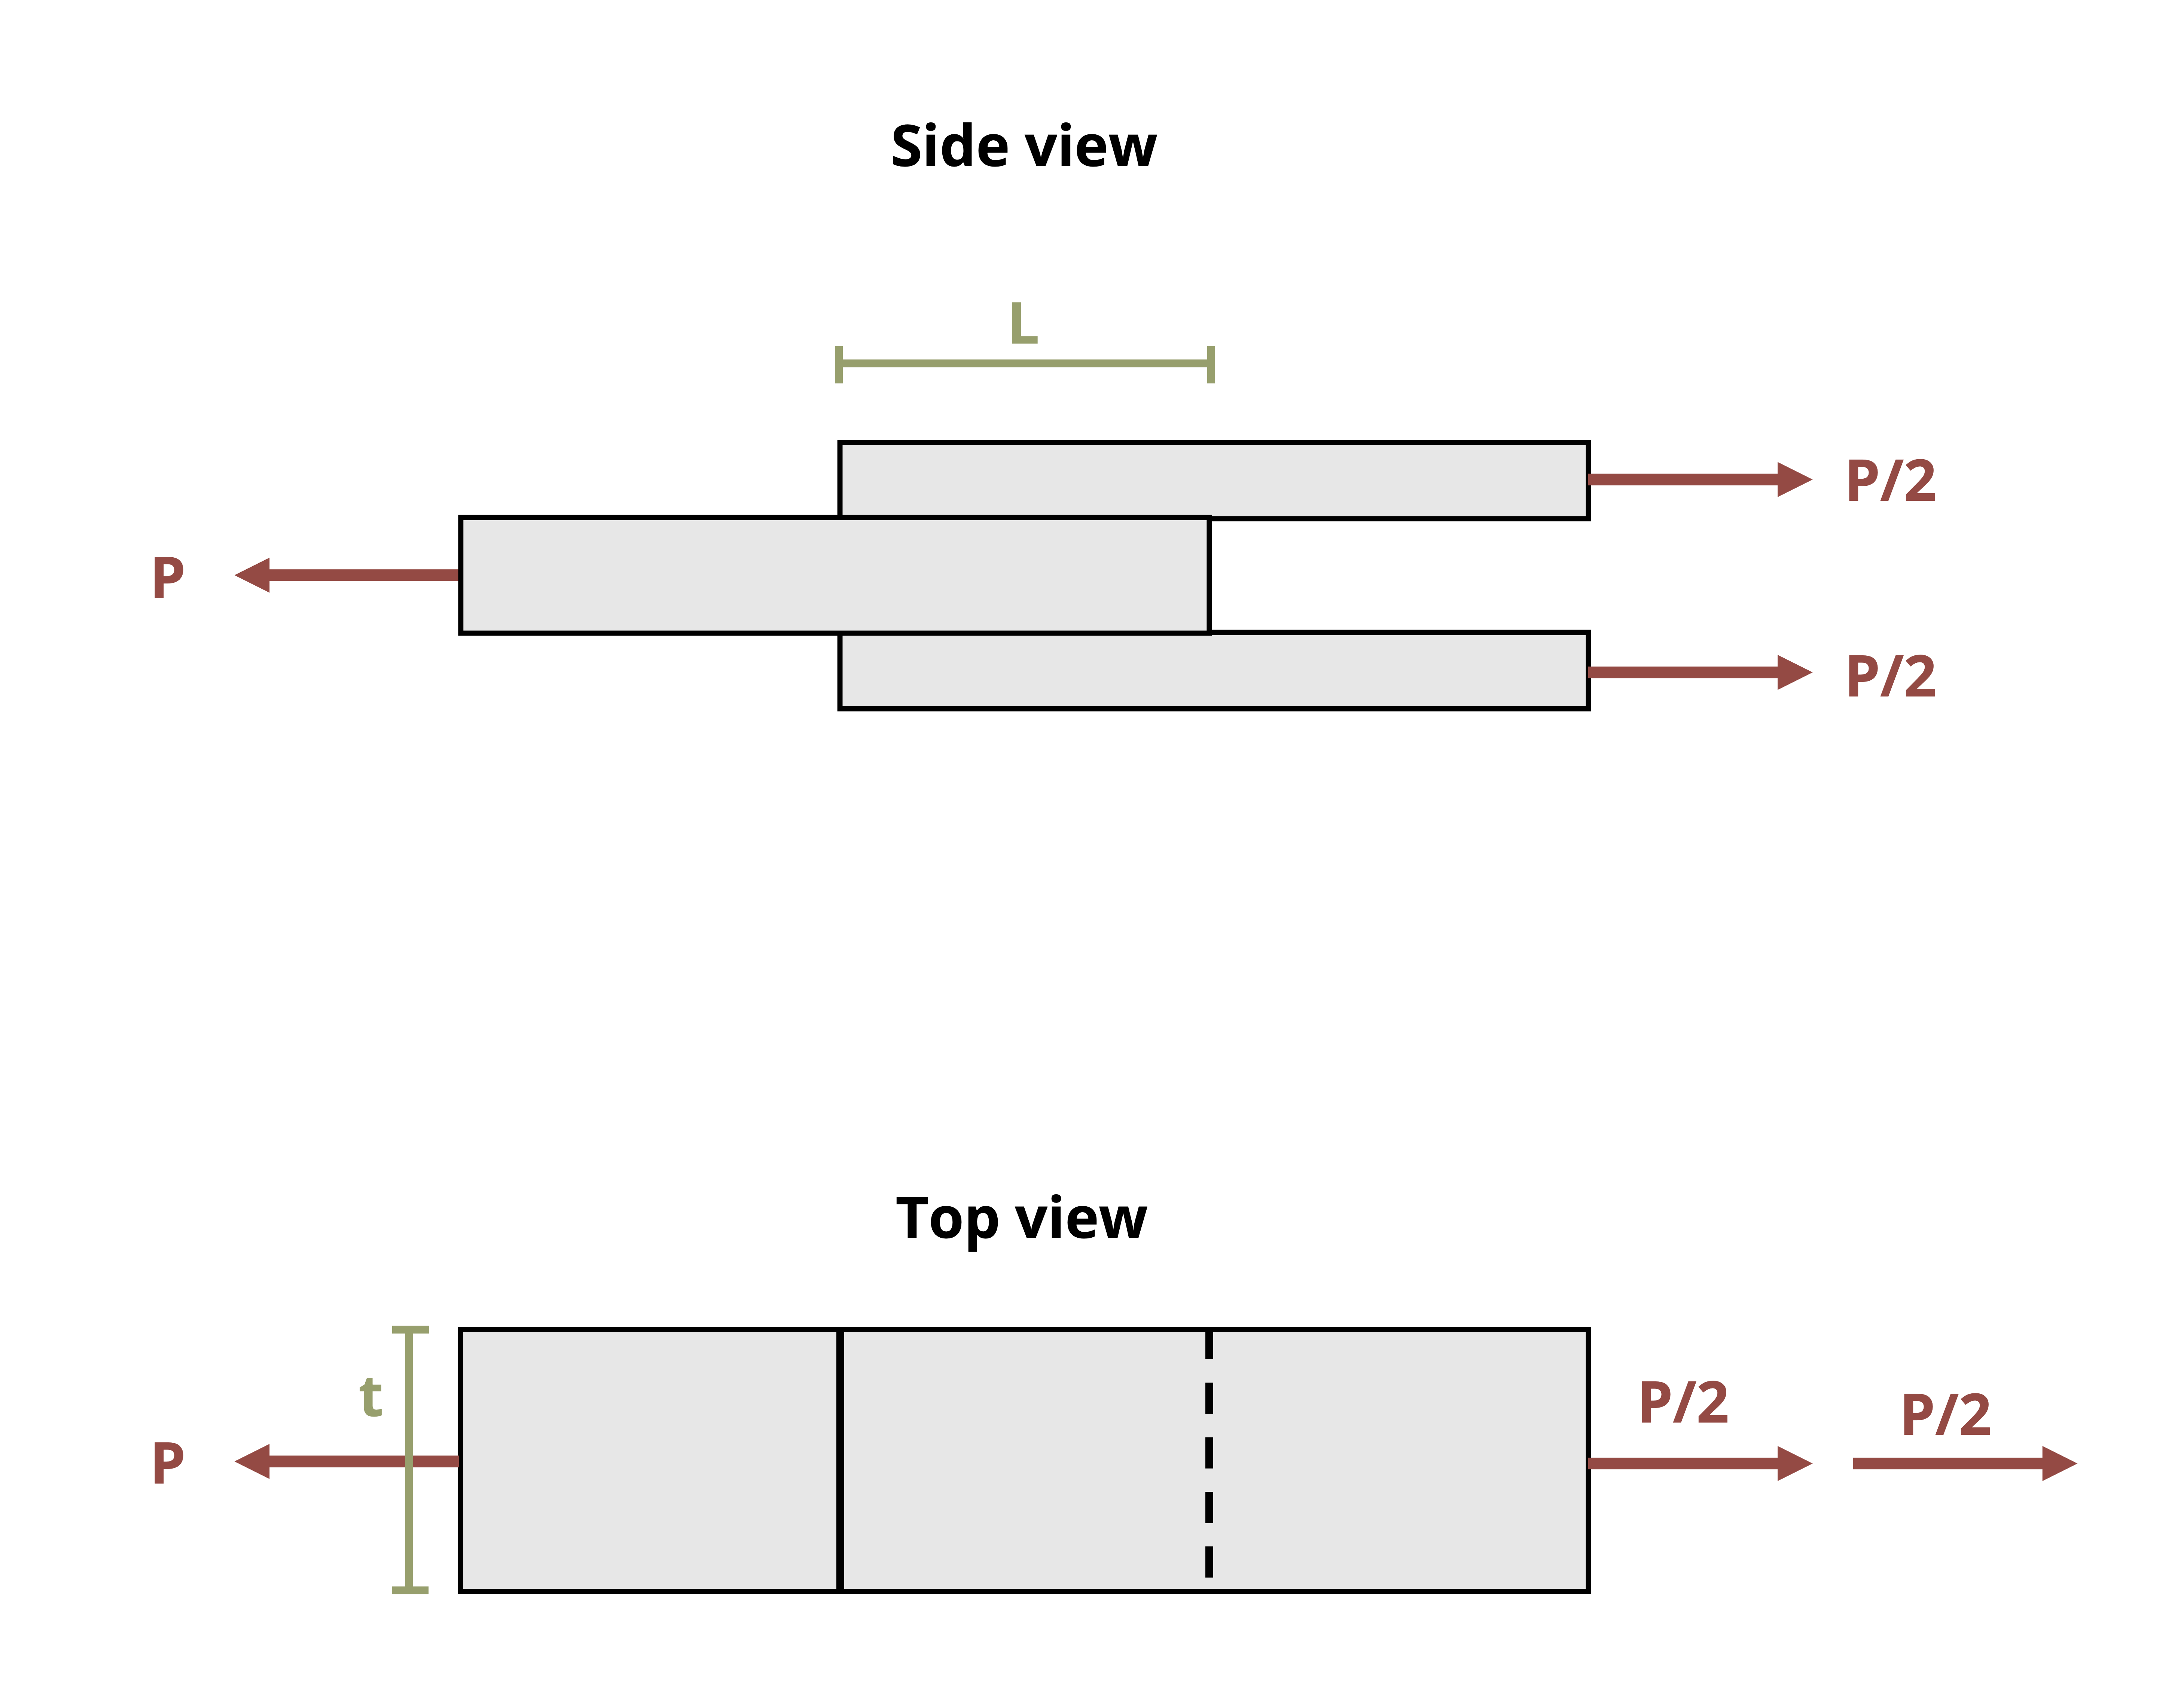
\includegraphics[keepaspectratio]{images/164.png}}
{[}Problem adapted from © Kurt Gramoll CC BY NC-SA 4.0{]}

\begin{Shaded}
\begin{Highlighting}[]
\NormalTok{\#| standalone: true}
\NormalTok{\#| viewerHeight: 600}
\NormalTok{\#| components: [viewer]}

\NormalTok{from shiny import App, render, ui, reactive}
\NormalTok{import random}
\NormalTok{import asyncio}
\NormalTok{import io}
\NormalTok{import math}
\NormalTok{import string}
\NormalTok{from datetime import datetime}
\NormalTok{from pathlib import Path}

\NormalTok{def generate\_random\_letters(length):}
\NormalTok{    \# Generate a random string of letters of specified length}
\NormalTok{    return \textquotesingle{}\textquotesingle{}.join(random.choice(string.ascii\_lowercase) for \_ in range(length))  }

\NormalTok{problem\_ID="164"}
\NormalTok{τfail=reactive.Value("\_\_")}
\NormalTok{L=reactive.Value("\_\_")}
\NormalTok{t=reactive.Value("\_\_")}

\NormalTok{attempts=["Timestamp,Attempt,Answer,Feedback\textbackslash{}n"]}

\NormalTok{app\_ui = ui.page\_fluid(}
\NormalTok{    ui.markdown("**Please enter your ID number from your instructor and click to generate your problem**"),}
\NormalTok{    ui.input\_text("ID","", placeholder="Enter ID Number Here"),}
\NormalTok{    ui.input\_action\_button("generate\_problem", "Generate Problem", class\_="btn{-}primary"),}
\NormalTok{    ui.markdown("**Problem Statement**"),}
\NormalTok{    ui.output\_ui("ui\_problem\_statement"),}
\NormalTok{    ui.input\_text("answer","Your Answer in units of kips", placeholder="Please enter your answer"),}
\NormalTok{    ui.input\_action\_button("submit", "Submit Answer", class\_="btn{-}primary"),}
\NormalTok{    ui.download\_button("download", "Download File to Submit", class\_="btn{-}success"),}
\NormalTok{)}


\NormalTok{def server(input, output, session):}
\NormalTok{    \# Initialize a counter for attempts}
\NormalTok{    attempt\_counter = reactive.Value(0)}

\NormalTok{    @output}
\NormalTok{    @render.ui}
\NormalTok{    def ui\_problem\_statement():}
\NormalTok{        return[ui.markdown(f"A double lap joint is glued together using glue with a shear stress failure strength of \{τfail()\} psi. If dimensions L = \{L()\} in. and t = \{t()\} in., what is the maximum load P that the joint can withstand? Assume the load is evenly distributed across the joint on both sides.")]}
    
\NormalTok{    @reactive.Effect}
\NormalTok{    @reactive.event(input.generate\_problem)}
\NormalTok{    def randomize\_vars():}
\NormalTok{        random.seed(input.ID())}
\NormalTok{        τfail.set(random.randrange(7000, 9000, 100))}
\NormalTok{        L.set(random.randrange(40, 100, 1)/10)}
\NormalTok{        t.set(random.randrange(40, 100, 1)/10)}
        

\NormalTok{    @reactive.Effect}
\NormalTok{    @reactive.event(input.submit)}
\NormalTok{    def \_():}
\NormalTok{        attempt\_counter.set(attempt\_counter() + 1)  \# Increment the attempt counter on each submission.}
    
\NormalTok{        A = L()*t()*2}
\NormalTok{        instr= (τfail()*A)/1000}
\NormalTok{        if math.isclose(float(input.answer()), instr, rel\_tol=0.01):}
\NormalTok{            check = "*Correct*"}
\NormalTok{            correct\_indicator = "JL"}
\NormalTok{        else:}
\NormalTok{            check = "*Not Correct.*"}
\NormalTok{            correct\_indicator = "JG"}

\NormalTok{        \# Generate random parts for the encoded attempt.}
\NormalTok{        random\_start = generate\_random\_letters(4)}
\NormalTok{        random\_middle = generate\_random\_letters(4)}
\NormalTok{        random\_end = generate\_random\_letters(4)}
\NormalTok{        encoded\_attempt = f"\{random\_start\}\{problem\_ID\}{-}\{random\_middle\}\{attempt\_counter()\}\{correct\_indicator\}{-}\{random\_end\}\{input.ID()\}"}

\NormalTok{        \# Store the most recent encoded attempt in a reactive value so it persists across submissions}
\NormalTok{        session.encoded\_attempt = reactive.Value(encoded\_attempt)}

\NormalTok{        \# Append the attempt data to the attempts list without the encoded attempt}
\NormalTok{        attempts.append(f"\{datetime.now()\}, \{attempt\_counter()\}, \{input.answer()\}, \{check\}\textbackslash{}n")}

\NormalTok{        \# Show feedback to the user.}
\NormalTok{        feedback = ui.markdown(f"Your answer of \{input.answer()\} is \{check\}.")}
\NormalTok{        m = ui.modal(}
\NormalTok{            feedback,}
\NormalTok{            title="Feedback",}
\NormalTok{            easy\_close=True}
\NormalTok{        )}
\NormalTok{        ui.modal\_show(m)}

\NormalTok{    @session.download(filename=lambda: f"Problem\_Log{-}\{problem\_ID\}{-}\{input.ID()\}.csv")}
\NormalTok{    async def download():}
\NormalTok{        \# Start the CSV with the encoded attempt (without label)}
\NormalTok{        final\_encoded = session.encoded\_attempt() if session.encoded\_attempt is not None else "No attempts"}
\NormalTok{        yield f"\{final\_encoded\}\textbackslash{}n\textbackslash{}n"}
        
\NormalTok{        \# Write the header for the remaining CSV data once}
\NormalTok{        yield "Timestamp,Attempt,Answer,Feedback\textbackslash{}n"}
        
\NormalTok{        \# Write the attempts data, ensure that the header from the attempts list is not written again}
\NormalTok{        for attempt in attempts[1:]:  \# Skip the first element which is the header}
\NormalTok{            await asyncio.sleep(0.25)  \# This delay may not be necessary; adjust as needed}
\NormalTok{            yield attempt}


\NormalTok{\# App installation}
\NormalTok{app = App(app\_ui, server)}
\end{Highlighting}
\end{Shaded}

\chapter*{Problem 2.22 - Average Shear
Stress}\label{problem-2.22---average-shear-stress}
\addcontentsline{toc}{chapter}{Problem 2.22 - Average Shear Stress}

\markboth{Problem 2.22 - Average Shear Stress}{Problem 2.22 - Average
Shear Stress}

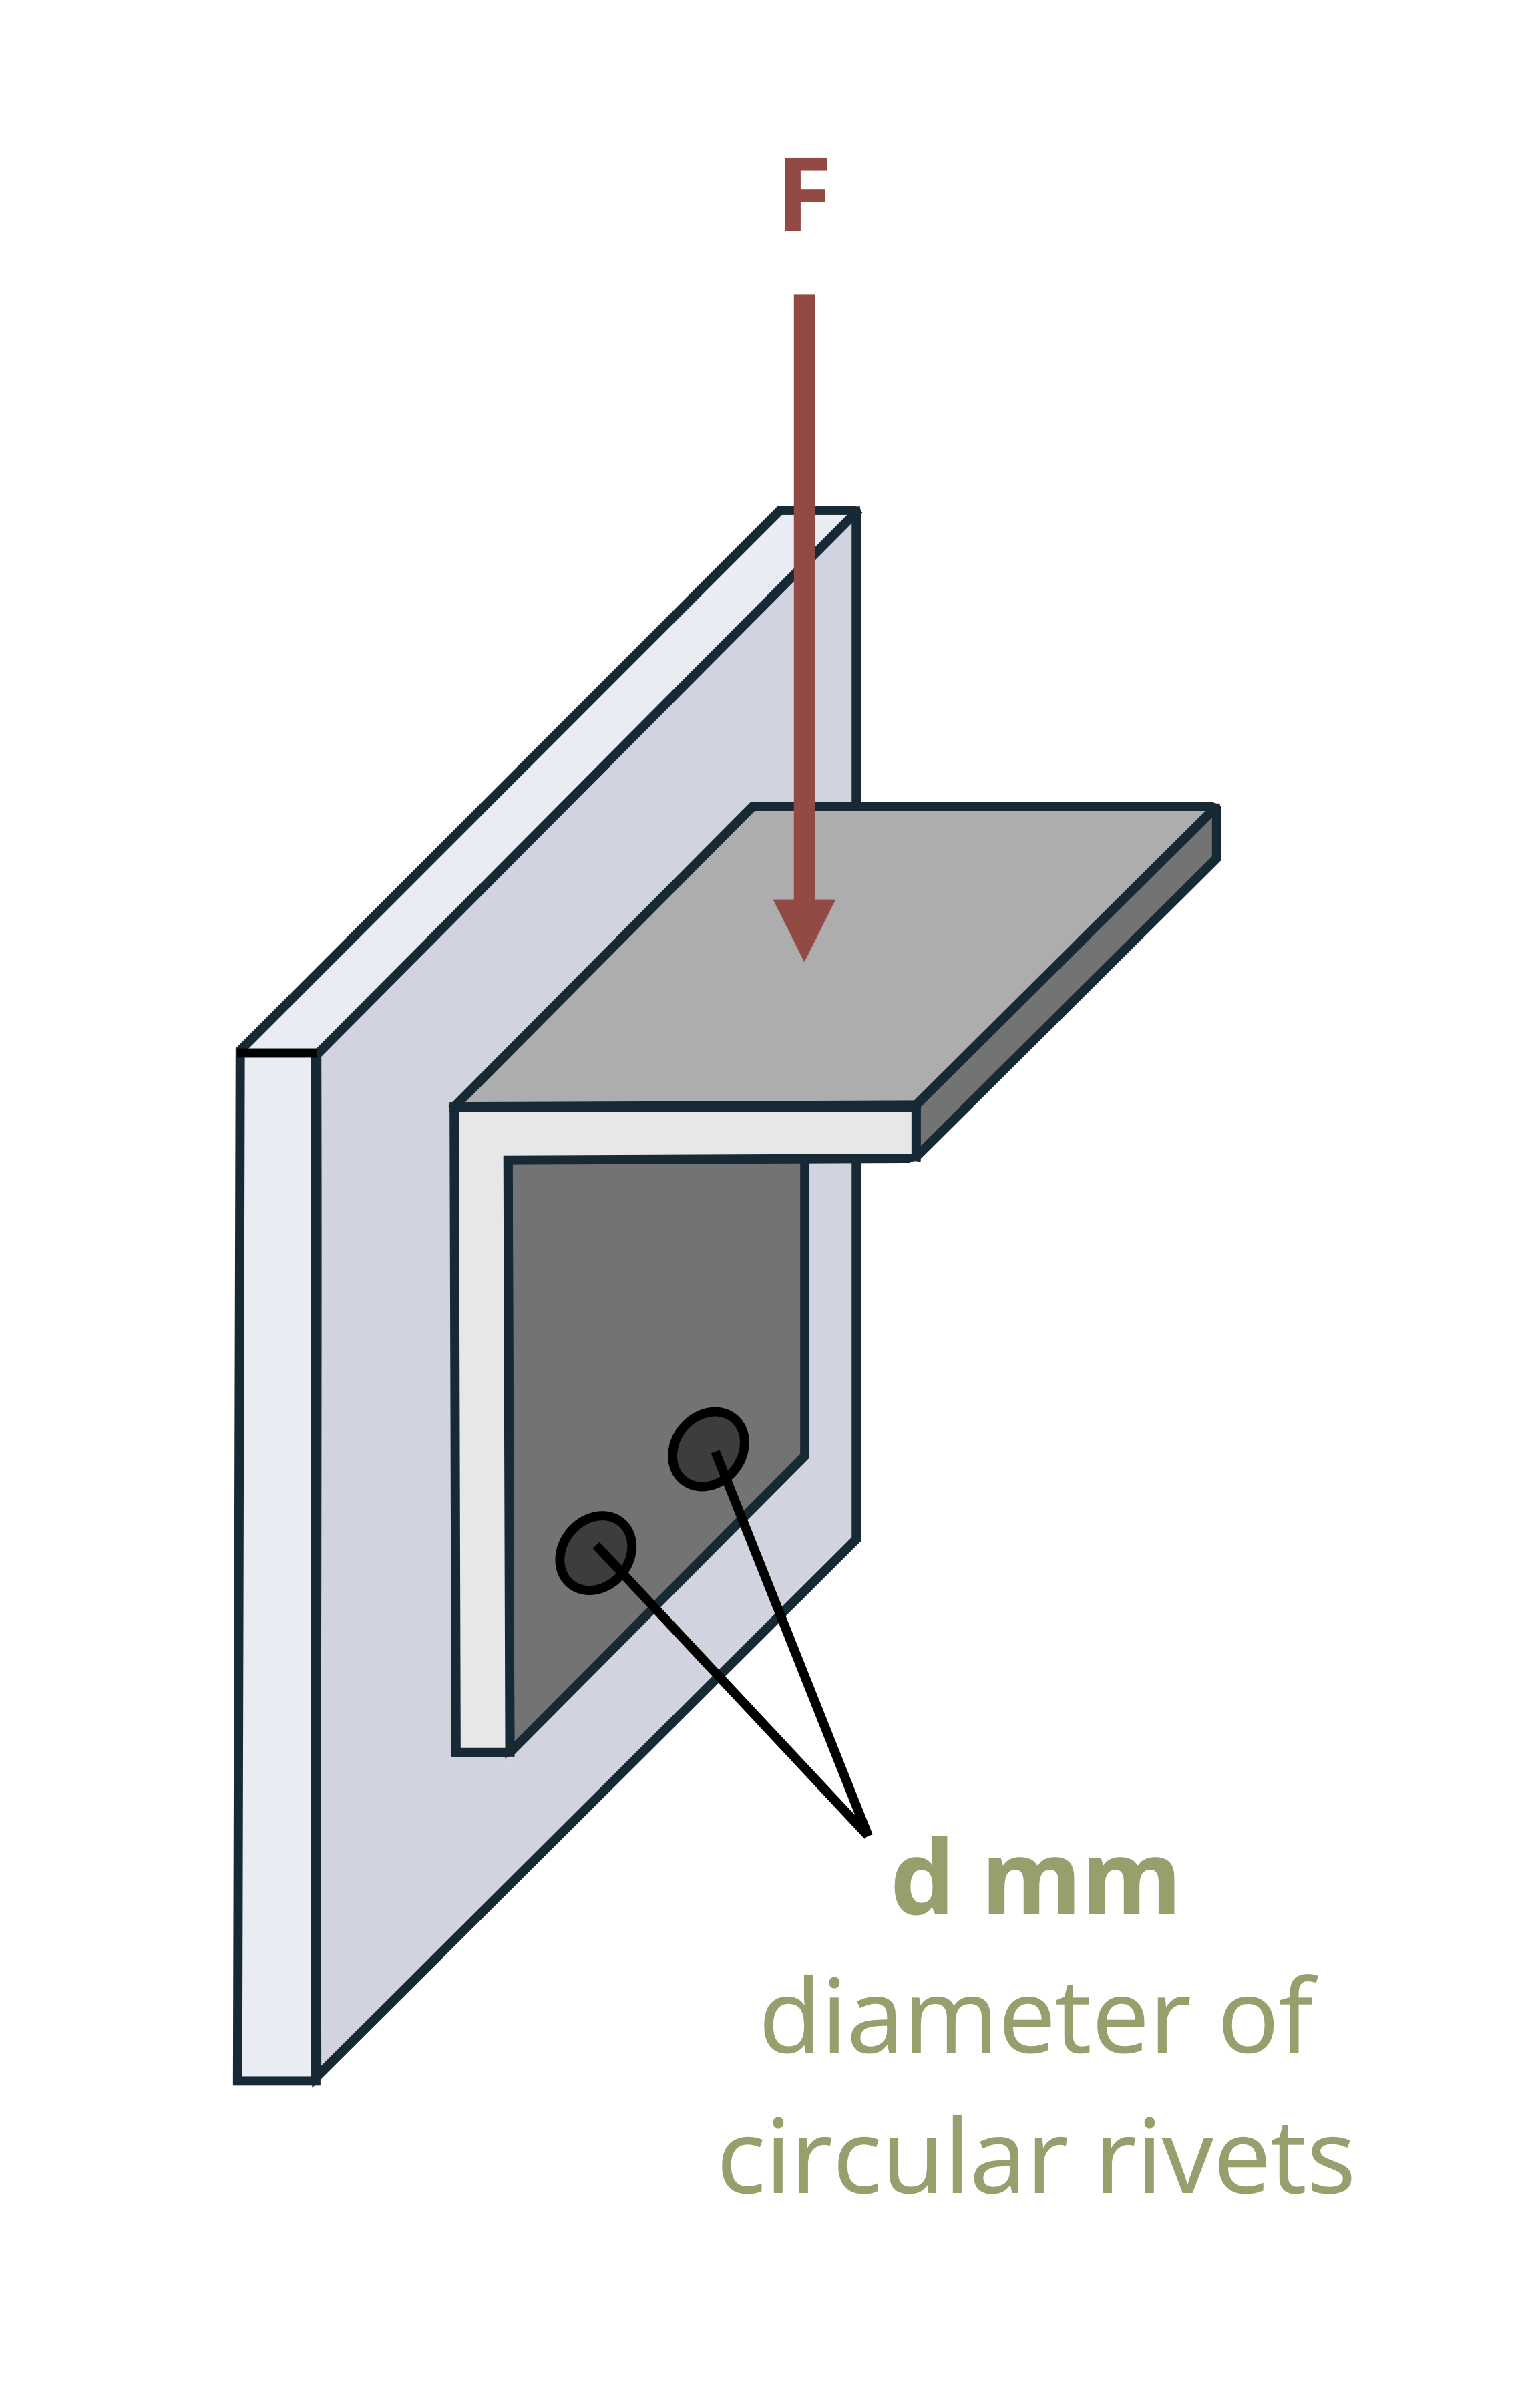
\includegraphics[width=10.09375in,height=\textheight,keepaspectratio]{images/165.png}
{[}Problem adapted from © Kurt Gramoll CC BY NC-SA 4.0{]}

\begin{Shaded}
\begin{Highlighting}[]
\NormalTok{\#| standalone: true}
\NormalTok{\#| viewerHeight: 600}
\NormalTok{\#| components: [viewer]}

\NormalTok{from shiny import App, render, ui, reactive}
\NormalTok{import random}
\NormalTok{import asyncio}
\NormalTok{import io}
\NormalTok{import math}
\NormalTok{import string}
\NormalTok{from datetime import datetime}
\NormalTok{from pathlib import Path}

\NormalTok{def generate\_random\_letters(length):}
\NormalTok{    \# Generate a random string of letters of specified length}
\NormalTok{    return \textquotesingle{}\textquotesingle{}.join(random.choice(string.ascii\_lowercase) for \_ in range(length))}

\NormalTok{problem\_ID="165"}
\NormalTok{F=reactive.Value("\_\_")}
\NormalTok{d=reactive.Value("\_\_")}


\NormalTok{attempts=["Timestamp,Attempt,Answer,Feedback\textbackslash{}n"]}

\NormalTok{app\_ui = ui.page\_fluid(}
\NormalTok{    ui.markdown("**Please enter your ID number from your instructor and click to generate your problem**"),}
\NormalTok{    ui.input\_text("ID","", placeholder="Enter ID Number Here"),}
\NormalTok{    ui.input\_action\_button("generate\_problem", "Generate Problem", class\_="btn{-}primary"),}
\NormalTok{    ui.markdown("**Problem Statement**"),}
\NormalTok{    ui.output\_ui("ui\_problem\_statement"),}
\NormalTok{    ui.input\_text("answer","Your Answer in units of MPa", placeholder="Please enter your answer"),}
\NormalTok{    ui.input\_action\_button("submit", "Submit Answer", class\_="btn{-}primary"),}
\NormalTok{    ui.download\_button("download", "Download File to Submit", class\_="btn{-}success"),}
\NormalTok{)}


\NormalTok{def server(input, output, session):}
\NormalTok{    \# Initialize a counter for attempts}
\NormalTok{    attempt\_counter = reactive.Value(0)}

\NormalTok{    @output}
\NormalTok{    @render.ui}
\NormalTok{    def ui\_problem\_statement():}
\NormalTok{        return[ui.markdown(f"A bracket is attached to a wall with two circular rivets of diameter d = \{d()\} mm. A load F = \{F()\} kN is applied in the center of the bracket. Assuming the load is split evenly between the two rivits, determine the shear stress in each rivet. ")]}
    
\NormalTok{    @reactive.Effect}
\NormalTok{    @reactive.event(input.generate\_problem)}
\NormalTok{    def randomize\_vars():}
\NormalTok{        random.seed(input.ID())}
\NormalTok{        F.set(random.randrange(30, 100, 1))}
\NormalTok{        d.set(random.randrange(10, 40, 1))}
        

\NormalTok{    @reactive.Effect}
\NormalTok{    @reactive.event(input.submit)}
\NormalTok{    def \_():}
\NormalTok{        attempt\_counter.set(attempt\_counter() + 1)  \# Increment the attempt counter on each submission.  }
      
\NormalTok{        A = math.pi*(d()/(1000*2))**2}
\NormalTok{        instr= ((F()/2)/A)/1000}
\NormalTok{        if math.isclose(float(input.answer()), instr, rel\_tol=0.01):}
\NormalTok{            check = "*Correct*"}
\NormalTok{            correct\_indicator = "JL"}
\NormalTok{        else:}
\NormalTok{            check = "*Not Correct.*"}
\NormalTok{            correct\_indicator = "JG"}

\NormalTok{        \# Generate random parts for the encoded attempt.}
\NormalTok{        random\_start = generate\_random\_letters(4)}
\NormalTok{        random\_middle = generate\_random\_letters(4)}
\NormalTok{        random\_end = generate\_random\_letters(4)}
\NormalTok{        encoded\_attempt = f"\{random\_start\}\{problem\_ID\}{-}\{random\_middle\}\{attempt\_counter()\}\{correct\_indicator\}{-}\{random\_end\}\{input.ID()\}"}

\NormalTok{        \# Store the most recent encoded attempt in a reactive value so it persists across submissions}
\NormalTok{        session.encoded\_attempt = reactive.Value(encoded\_attempt)}

\NormalTok{        \# Append the attempt data to the attempts list without the encoded attempt}
\NormalTok{        attempts.append(f"\{datetime.now()\}, \{attempt\_counter()\}, \{input.answer()\}, \{check\}\textbackslash{}n")}

\NormalTok{        \# Show feedback to the user.}
\NormalTok{        feedback = ui.markdown(f"Your answer of \{input.answer()\} is \{check\}.")}
\NormalTok{        m = ui.modal(}
\NormalTok{            feedback,}
\NormalTok{            title="Feedback",}
\NormalTok{            easy\_close=True}
\NormalTok{        )}
\NormalTok{        ui.modal\_show(m)}

\NormalTok{    @session.download(filename=lambda: f"Problem\_Log{-}\{problem\_ID\}{-}\{input.ID()\}.csv")}
\NormalTok{    async def download():}
\NormalTok{        \# Start the CSV with the encoded attempt (without label)}
\NormalTok{        final\_encoded = session.encoded\_attempt() if session.encoded\_attempt is not None else "No attempts"}
\NormalTok{        yield f"\{final\_encoded\}\textbackslash{}n\textbackslash{}n"}
        
\NormalTok{        \# Write the header for the remaining CSV data once}
\NormalTok{        yield "Timestamp,Attempt,Answer,Feedback\textbackslash{}n"}
        
\NormalTok{        \# Write the attempts data, ensure that the header from the attempts list is not written again}
\NormalTok{        for attempt in attempts[1:]:  \# Skip the first element which is the header}
\NormalTok{            await asyncio.sleep(0.25)  \# This delay may not be necessary; adjust as needed}
\NormalTok{            yield attempt}


\NormalTok{\# App installation}
\NormalTok{app = App(app\_ui, server)}
\end{Highlighting}
\end{Shaded}

\chapter*{Problem 2.23 - Average Shear
Stress}\label{problem-2.23---average-shear-stress}
\addcontentsline{toc}{chapter}{Problem 2.23 - Average Shear Stress}

\markboth{Problem 2.23 - Average Shear Stress}{Problem 2.23 - Average
Shear Stress}

\begin{figure}[H]

{\centering \pandocbounded{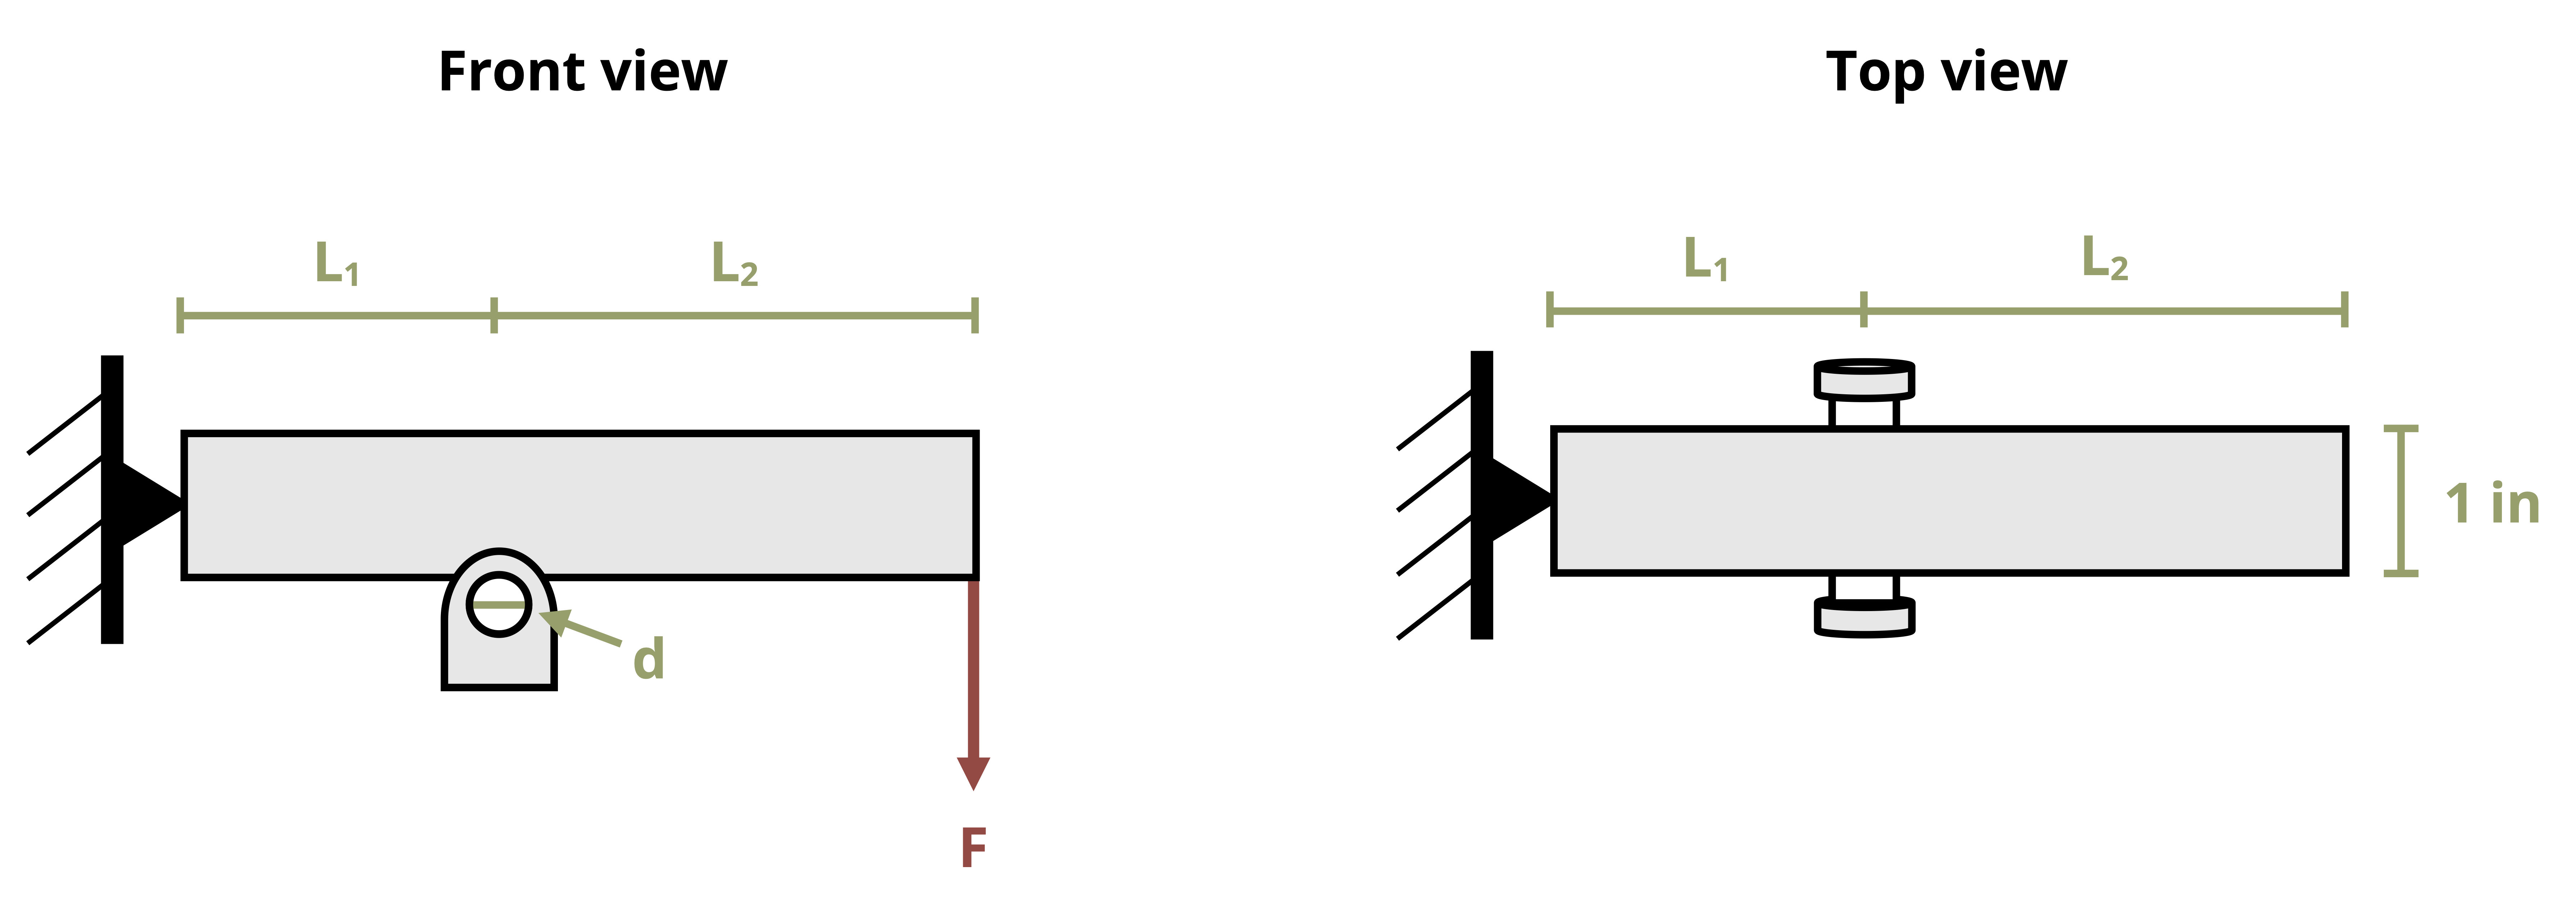
\includegraphics[keepaspectratio]{images/168.png}}

}

\caption{Figure 1: A square bar of length is pinned at one end and rests
on a circular rod.}

\end{figure}%

{[}Problem adapted from © Kurt Gramoll CC BY NC-SA 4.0{]}

\begin{Shaded}
\begin{Highlighting}[]
\NormalTok{\#| standalone: true}
\NormalTok{\#| viewerHeight: 600}
\NormalTok{\#| components: [viewer]}

\NormalTok{from shiny import App, render, ui, reactive}
\NormalTok{import random}
\NormalTok{import asyncio}
\NormalTok{import io}
\NormalTok{import math}
\NormalTok{import string}
\NormalTok{from datetime import datetime}
\NormalTok{from pathlib import Path}

\NormalTok{def generate\_random\_letters(length):}
\NormalTok{    \# Generate a random string of letters of specified length}
\NormalTok{    return \textquotesingle{}\textquotesingle{}.join(random.choice(string.ascii\_lowercase) for \_ in range(length)) }

\NormalTok{problem\_ID="168"}
\NormalTok{L1=reactive.Value("\_\_")}
\NormalTok{L2=reactive.Value("\_\_")}
\NormalTok{d=reactive.Value("\_\_")}
\NormalTok{F=reactive.Value("\_\_")}

\NormalTok{attempts=["Timestamp,Attempt,Answer,Feedback\textbackslash{}n"]}

\NormalTok{app\_ui = ui.page\_fluid(}
\NormalTok{    ui.markdown("**Please enter your ID number from your instructor and click to generate your problem**"),}
\NormalTok{    ui.input\_text("ID","", placeholder="Enter ID Number Here"),}
\NormalTok{    ui.input\_action\_button("generate\_problem", "Generate Problem", class\_="btn{-}primary"),}
\NormalTok{    ui.markdown("**Problem Statement**"),}
\NormalTok{    ui.output\_ui("ui\_problem\_statement"),}
\NormalTok{    ui.input\_text("answer","Your Answer in units of psi", placeholder="Please enter your answer"),}
\NormalTok{    ui.input\_action\_button("submit", "Submit Answer", class\_="btn{-}primary"),}
\NormalTok{    ui.download\_button("download", "Download File to Submit", class\_="btn{-}success"),}
\NormalTok{)}

\NormalTok{def server(input, output, session):}
\NormalTok{    \# Initialize a counter for attempts}
\NormalTok{    attempt\_counter = reactive.Value(0)}

\NormalTok{    @output}
\NormalTok{    @render.ui}
\NormalTok{    def ui\_problem\_statement():}
\NormalTok{        return[ui.markdown(f"A square bar of length L\textless{}sub\textgreater{}1\textless{}/sub\textgreater{} = \{L1()\} in. and L\textless{}sub\textgreater{}2\textless{}/sub\textgreater{} = \{L2()\} in. is pinned at one end and rests on a circular rod of diameter d = \{d()\} in. A force F = \{F()\} lb is applied at the free end. What is the average shear stress in the circular rod? ")]}
    
\NormalTok{    @reactive.Effect}
\NormalTok{    @reactive.event(input.generate\_problem)}
\NormalTok{    def randomize\_vars():}
\NormalTok{        random.seed(input.ID())}
\NormalTok{        L1.set(random.randrange(50, 150, 1)/10)}
\NormalTok{        L2.set(round(L1() * 1.4, 1))}
\NormalTok{        d.set(random.randrange(4, 9, 1)/10)}
\NormalTok{        F.set(random.randrange(30, 100, 1))}

\NormalTok{    @reactive.Effect}
\NormalTok{    @reactive.event(input.submit)}
\NormalTok{    def \_():}
\NormalTok{        attempt\_counter.set(attempt\_counter() + 1)  \# Increment the attempt counter on each submission.}
    
\NormalTok{        M = F()*(L1()+L2())}
\NormalTok{        R = M/L1()}
\NormalTok{        A = math.pi*(d()/2)**2}
\NormalTok{        instr= R/(2*A)}
\NormalTok{        if math.isclose(float(input.answer()), instr, rel\_tol=0.01):}
\NormalTok{            check = "*Correct*"}
\NormalTok{            correct\_indicator = "JL"}
\NormalTok{        else:}
\NormalTok{            check = "*Not Correct.*"}
\NormalTok{            correct\_indicator = "JG"}

\NormalTok{        \# Generate random parts for the encoded attempt.}
\NormalTok{        random\_start = generate\_random\_letters(4)}
\NormalTok{        random\_middle = generate\_random\_letters(4)}
\NormalTok{        random\_end = generate\_random\_letters(4)}
\NormalTok{        encoded\_attempt = f"\{random\_start\}\{problem\_ID\}{-}\{random\_middle\}\{attempt\_counter()\}\{correct\_indicator\}{-}\{random\_end\}\{input.ID()\}"}

\NormalTok{        \# Store the most recent encoded attempt in a reactive value so it persists across submissions}
\NormalTok{        session.encoded\_attempt = reactive.Value(encoded\_attempt)}

\NormalTok{        \# Append the attempt data to the attempts list without the encoded attempt}
\NormalTok{        attempts.append(f"\{datetime.now()\}, \{attempt\_counter()\}, \{input.answer()\}, \{check\}\textbackslash{}n")}

\NormalTok{        \# Show feedback to the user.}
\NormalTok{        feedback = ui.markdown(f"Your answer of \{input.answer()\} is \{check\}.")}
\NormalTok{        m = ui.modal(}
\NormalTok{            feedback,}
\NormalTok{            title="Feedback",}
\NormalTok{            easy\_close=True}
\NormalTok{        )}
\NormalTok{        ui.modal\_show(m)}

\NormalTok{    @session.download(filename=lambda: f"Problem\_Log{-}\{problem\_ID\}{-}\{input.ID()\}.csv")}
\NormalTok{    async def download():}
\NormalTok{        \# Start the CSV with the encoded attempt (without label)}
\NormalTok{        final\_encoded = session.encoded\_attempt() if session.encoded\_attempt is not None else "No attempts"}
\NormalTok{        yield f"\{final\_encoded\}\textbackslash{}n\textbackslash{}n"}
        
\NormalTok{        \# Write the header for the remaining CSV data once}
\NormalTok{        yield "Timestamp,Attempt,Answer,Feedback\textbackslash{}n"}
        
\NormalTok{        \# Write the attempts data, ensure that the header from the attempts list is not written again}
\NormalTok{        for attempt in attempts[1:]:  \# Skip the first element which is the header}
\NormalTok{            await asyncio.sleep(0.25)  \# This delay may not be necessary; adjust as needed}
\NormalTok{            yield attempt}

\NormalTok{\# App installation}
\NormalTok{app = App(app\_ui, server)}
\end{Highlighting}
\end{Shaded}

\chapter*{Problem 2.38 - Bearing
Stress}\label{problem-2.38---bearing-stress}
\addcontentsline{toc}{chapter}{Problem 2.38 - Bearing Stress}

\markboth{Problem 2.38 - Bearing Stress}{Problem 2.38 - Bearing Stress}

\pandocbounded{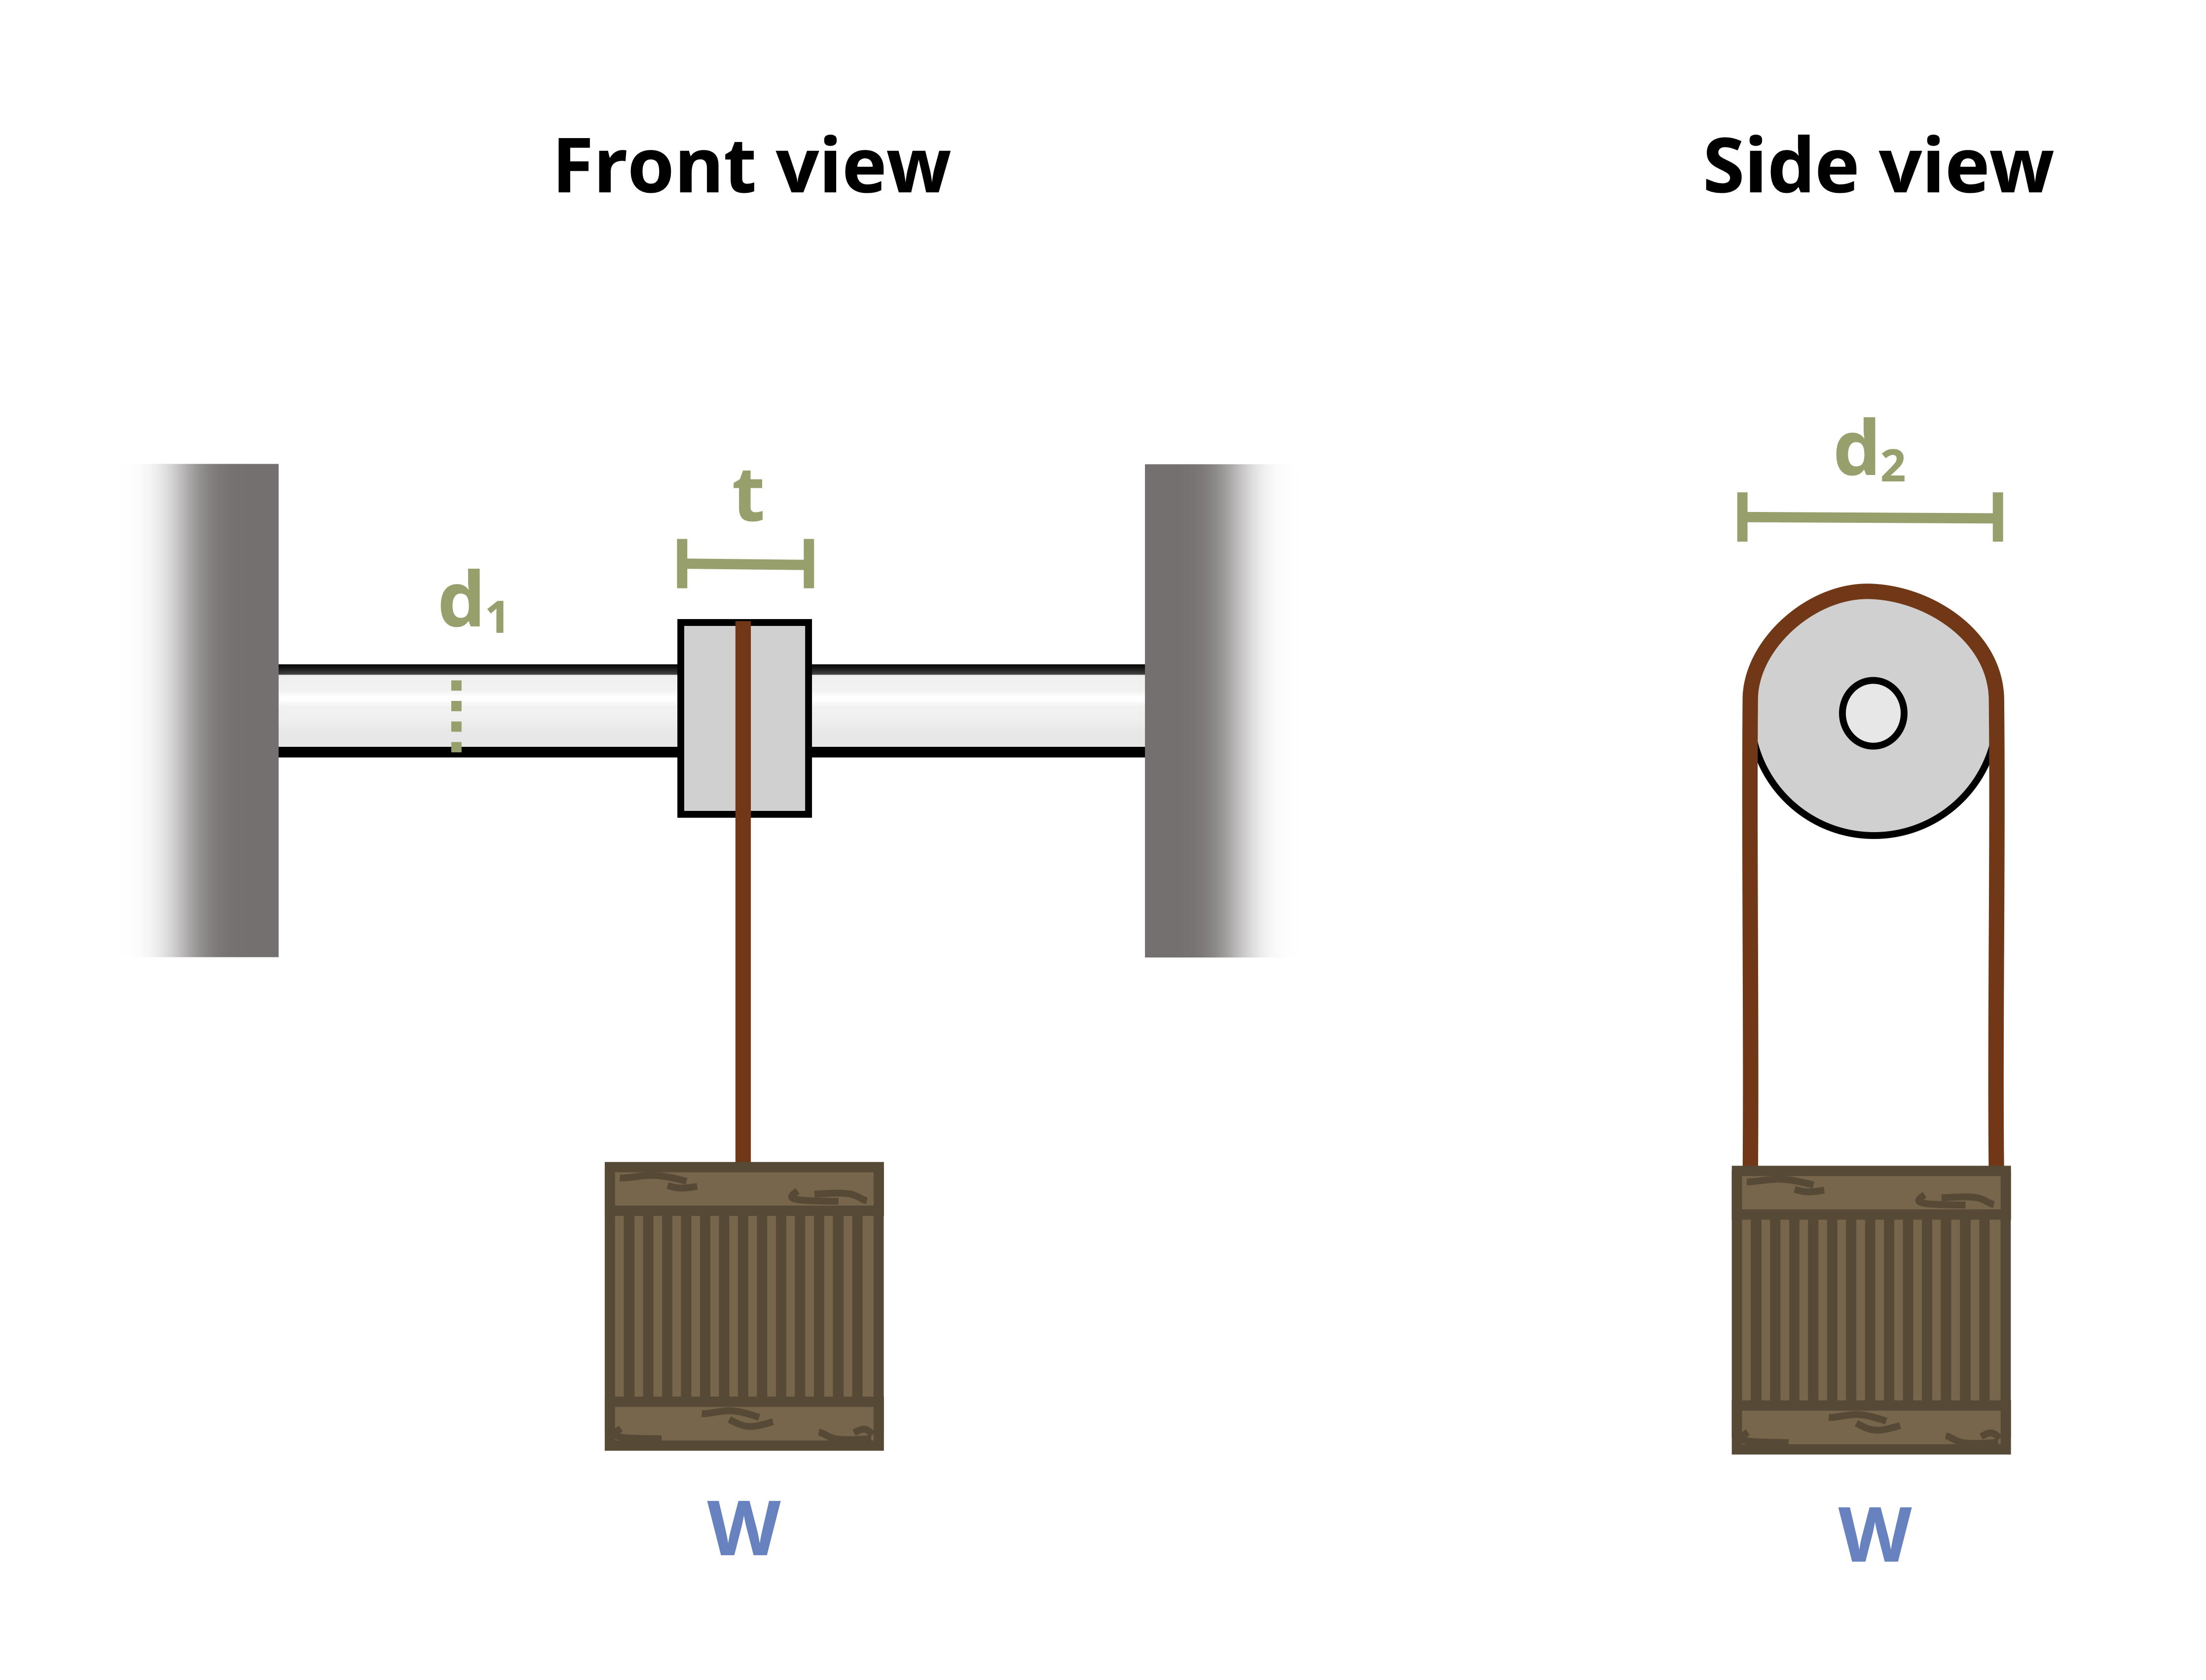
\includegraphics[keepaspectratio]{images/166.png}}
{[}Problem adapted from © Kurt Gramoll CC BY NC-SA 4.0{]}

\begin{Shaded}
\begin{Highlighting}[]
\NormalTok{\#| standalone: true}
\NormalTok{\#| viewerHeight: 600}
\NormalTok{\#| components: [viewer]}
\NormalTok{from shiny import App, render, ui, reactive}
\NormalTok{import random}
\NormalTok{import asyncio}
\NormalTok{import io}
\NormalTok{import math}
\NormalTok{import string}
\NormalTok{from datetime import datetime}
\NormalTok{from pathlib import Path}

\NormalTok{def generate\_random\_letters(length):}
\NormalTok{    \# Generate a random string of letters of specified length}
\NormalTok{    return \textquotesingle{}\textquotesingle{}.join(random.choice(string.ascii\_lowercase) for \_ in range(length))}

\NormalTok{problem\_ID="166"}
\NormalTok{W=reactive.Value("\_\_")}
\NormalTok{d1=reactive.Value("\_\_")}
\NormalTok{d2=reactive.Value("\_\_")}
\NormalTok{t=reactive.Value("\_\_")}
\NormalTok{attempts=["Timestamp,Attempt,Answer,Feedback\textbackslash{}n"]}

\NormalTok{app\_ui = ui.page\_fluid(}
\NormalTok{    ui.markdown("**Please enter your ID number from your instructor and click to generate your problem**"),}
\NormalTok{    ui.input\_text("ID","", placeholder="Enter ID Number Here"),}
\NormalTok{    ui.input\_action\_button("generate\_problem", "Generate Problem", class\_="btn{-}primary"),}
\NormalTok{    ui.markdown("**Problem Statement**"),}
\NormalTok{    ui.output\_ui("ui\_problem\_statement"),}
\NormalTok{    ui.input\_text("answer","Your Answer in units of ksi", placeholder="Please enter your answer"),}
\NormalTok{    ui.input\_action\_button("submit", "Submit Answer", class\_="btn{-}primary"),}
\NormalTok{    ui.download\_button("download", "Download File to Submit", class\_="btn{-}success"),}
\NormalTok{)}


\NormalTok{def server(input, output, session):}
\NormalTok{    \# Initialize a counter for attempts}
\NormalTok{    attempt\_counter = reactive.Value(0)}
    
\NormalTok{    @output}
\NormalTok{    @render.ui}
\NormalTok{    def ui\_problem\_statement():}
\NormalTok{        return[ui.markdown(f"A crate of weight \{W()\} = lb hangs from a solid circular metal rod of diameter \{d1()\} = in.. The cable is wrapped around a support collar of diameter \{d2()\} = in. and thickness \{t()\} = in. to evenly distribute the cable load. What is the bearing stress on the support collar due to the rod? ")]}
    
\NormalTok{    @reactive.Effect}
\NormalTok{    @reactive.event(input.generate\_problem)}
\NormalTok{    def randomize\_vars():}
\NormalTok{        random.seed(input.ID())}
\NormalTok{        W.set(random.randrange(4000, 9000, 100))}
\NormalTok{        d1.set(random.randrange(5, 30, 1)/10)}
\NormalTok{        d2.set(d1()*3)}
\NormalTok{        t.set(d1()*2)}
\NormalTok{    @reactive.Effect}
\NormalTok{    @reactive.event(input.submit)}
\NormalTok{    def \_():}
        
\NormalTok{        instr= W()/(d1()*t()*1000)}
        
\NormalTok{        if math.isclose(float(input.answer()), instr, rel\_tol=0.01):}
\NormalTok{            check = "*Correct*"}
\NormalTok{            correct\_indicator = "JL"}
\NormalTok{        else:}
\NormalTok{            check = "*Not Correct.*"}
\NormalTok{            correct\_indicator = "JG"}

\NormalTok{        \# Generate random parts for the encoded attempt.}
\NormalTok{        random\_start = generate\_random\_letters(4)}
\NormalTok{        random\_middle = generate\_random\_letters(4)}
\NormalTok{        random\_end = generate\_random\_letters(4)}
\NormalTok{        encoded\_attempt = f"\{random\_start\}\{problem\_ID\}{-}\{random\_middle\}\{attempt\_counter()\}\{correct\_indicator\}{-}\{random\_end\}\{input.ID()\}"}

\NormalTok{        \# Store the most recent encoded attempt in a reactive value so it persists across submissions}
\NormalTok{        session.encoded\_attempt = reactive.Value(encoded\_attempt)}

\NormalTok{        \# Append the attempt data to the attempts list without the encoded attempt}
\NormalTok{        attempts.append(f"\{datetime.now()\}, \{attempt\_counter()\}, \{input.answer()\}, \{check\}\textbackslash{}n")}

\NormalTok{        \# Show feedback to the user.}
\NormalTok{        feedback = ui.markdown(f"Your answer of \{input.answer()\} is \{check\}.")}
\NormalTok{        m = ui.modal(}
\NormalTok{            feedback,}
\NormalTok{            title="Feedback",}
\NormalTok{            easy\_close=True}
\NormalTok{        )}
\NormalTok{        ui.modal\_show(m)}

\NormalTok{    @session.download(filename=lambda: f"Problem\_Log{-}\{problem\_ID\}{-}\{input.ID()\}.csv")}
\NormalTok{    async def download():}
\NormalTok{        \# Start the CSV with the encoded attempt (without label)}
\NormalTok{        final\_encoded = session.encoded\_attempt() if session.encoded\_attempt is not None else "No attempts"}
\NormalTok{        yield f"\{final\_encoded\}\textbackslash{}n\textbackslash{}n"}
        
\NormalTok{        \# Write the header for the remaining CSV data once}
\NormalTok{        yield "Timestamp,Attempt,Answer,Feedback\textbackslash{}n"}
        
\NormalTok{        \# Write the attempts data, ensure that the header from the attempts list is not written again}
\NormalTok{        for attempt in attempts[1:]:  \# Skip the first element which is the header}
\NormalTok{            await asyncio.sleep(0.25)  \# This delay may not be necessary; adjust as needed}
\NormalTok{            yield attempt}


\NormalTok{\# App installation}
\NormalTok{app = App(app\_ui, server)}
\end{Highlighting}
\end{Shaded}

\chapter*{Problem 2.39 - Bearing
Stress}\label{problem-2.39---bearing-stress}
\addcontentsline{toc}{chapter}{Problem 2.39 - Bearing Stress}

\markboth{Problem 2.39 - Bearing Stress}{Problem 2.39 - Bearing Stress}

\begin{figure}[H]

{\centering \pandocbounded{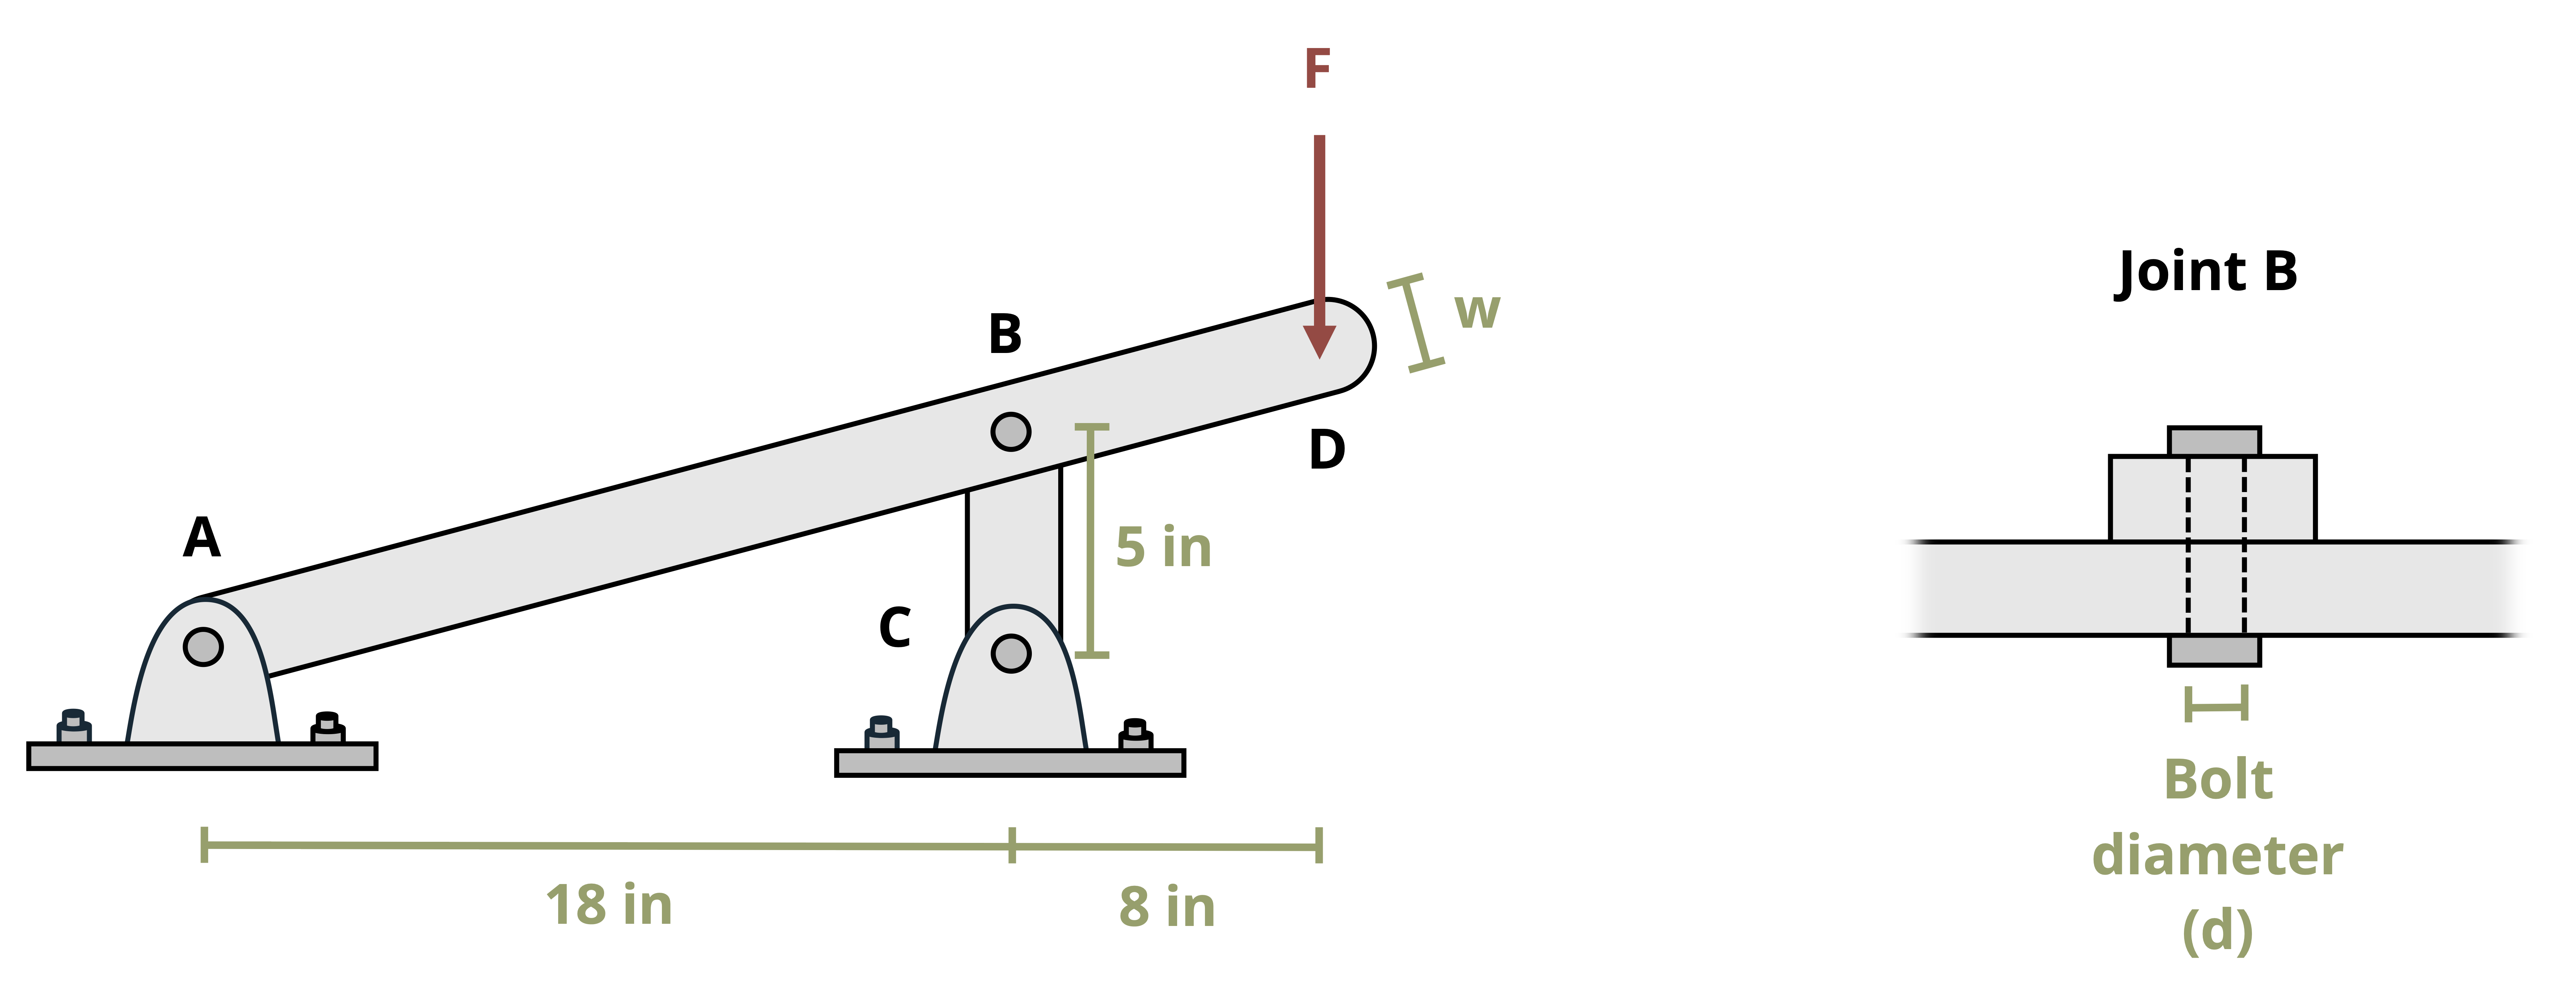
\includegraphics[keepaspectratio]{images/180.png}}

}

\caption{Figure 1: A link mechanism is connected with pins.}

\end{figure}%

{[}Problem adapted from © Kurt Gramoll CC BY NC-SA 4.0{]}

\begin{Shaded}
\begin{Highlighting}[]
\NormalTok{\#| standalone: true}
\NormalTok{\#| viewerHeight: 600}
\NormalTok{\#| components: [viewer]}

\NormalTok{from shiny import App, render, ui, reactive}
\NormalTok{import random}
\NormalTok{import asyncio}
\NormalTok{import io}
\NormalTok{import math}
\NormalTok{import string}
\NormalTok{from datetime import datetime}
\NormalTok{from pathlib import Path}

\NormalTok{def generate\_random\_letters(length):}
\NormalTok{    \# Generate a random string of letters of specified length}
\NormalTok{    return \textquotesingle{}\textquotesingle{}.join(random.choice(string.ascii\_lowercase) for \_ in range(length)) }

\NormalTok{problem\_ID="180"}
\NormalTok{F=reactive.Value("\_\_")}
\NormalTok{d=reactive.Value("\_\_")}
\NormalTok{t=reactive.Value("\_\_")}
\NormalTok{w=reactive.Value("\_\_")}



\NormalTok{attempts=["Timestamp,Attempt,Answer,Feedback\textbackslash{}n"]}

\NormalTok{app\_ui = ui.page\_fluid(}
\NormalTok{    ui.markdown("**Please enter your ID number from your instructor and click to generate your problem**"),}
\NormalTok{    ui.input\_text("ID","", placeholder="Enter ID Number Here"),}
\NormalTok{    ui.input\_action\_button("generate\_problem", "Generate Problem", class\_="btn{-}primary"),}
\NormalTok{    ui.markdown("**Problem Statement**"),}
\NormalTok{    ui.output\_ui("ui\_problem\_statement"),}
\NormalTok{    ui.input\_text("answer","Your Answer in units of ksi", placeholder="Please enter your answer"),}
\NormalTok{    ui.input\_action\_button("submit", "Submit Answer", class\_="btn{-}primary"),}
\NormalTok{    ui.download\_button("download", "Download File to Submit", class\_="btn{-}success"),}
\NormalTok{)}


\NormalTok{def server(input, output, session):}
\NormalTok{    \# Initialize a counter for attempts}
\NormalTok{    attempt\_counter = reactive.Value(0)  }
  
\NormalTok{    @output}
\NormalTok{    @render.ui}
\NormalTok{    def ui\_problem\_statement():}
\NormalTok{        return[ui.markdown(f"A link mechanism is connected with pins of diameter d = \{d()\} in. A force F = \{F()\} lb is applied to the mechanism as shown. The mechanism has width w = \{w()\} in. and thickness t = \{t()\} in. What is the bearing stress in member BC at joint B due to the pin at B? ")]}
    
\NormalTok{    @reactive.Effect}
\NormalTok{    @reactive.event(input.generate\_problem)}
\NormalTok{    def randomize\_vars():}
\NormalTok{        random.seed(input.ID())}
\NormalTok{        F.set(random.randrange(200, 900, 10))}
\NormalTok{        d.set(random.randrange(20, 150, 10)/100)}
\NormalTok{        t.set(random.randrange(2, 10, 1)/10)}
\NormalTok{        w.set(round(d()*2, 2))}
        

\NormalTok{    @reactive.Effect}
\NormalTok{    @reactive.event(input.submit)}
\NormalTok{    def \_():}
\NormalTok{        attempt\_counter.set(attempt\_counter() + 1)  \# Increment the attempt counter on each submission.}
\NormalTok{        Fb=((18+8)*F())/18}
\NormalTok{        instr= Fb/(d()*t())/1000}
\NormalTok{        if math.isclose(float(input.answer()), instr, rel\_tol=0.01):}
\NormalTok{            check = "*Correct*"}
\NormalTok{            correct\_indicator = "JL"}
\NormalTok{        else:}
\NormalTok{            check = "*Not Correct.*"}
\NormalTok{            correct\_indicator = "JG"}

\NormalTok{        \# Generate random parts for the encoded attempt.}
\NormalTok{        random\_start = generate\_random\_letters(4)}
\NormalTok{        random\_middle = generate\_random\_letters(4)}
\NormalTok{        random\_end = generate\_random\_letters(4)}
\NormalTok{        encoded\_attempt = f"\{random\_start\}\{problem\_ID\}{-}\{random\_middle\}\{attempt\_counter()\}\{correct\_indicator\}{-}\{random\_end\}\{input.ID()\}"}

\NormalTok{        \# Store the most recent encoded attempt in a reactive value so it persists across submissions}
\NormalTok{        session.encoded\_attempt = reactive.Value(encoded\_attempt)}

\NormalTok{        \# Append the attempt data to the attempts list without the encoded attempt}
\NormalTok{        attempts.append(f"\{datetime.now()\}, \{attempt\_counter()\}, \{input.answer()\}, \{check\}\textbackslash{}n")}

\NormalTok{        \# Show feedback to the user.}
\NormalTok{        feedback = ui.markdown(f"Your answer of \{input.answer()\} is \{check\}.")}
\NormalTok{        m = ui.modal(}
\NormalTok{            feedback,}
\NormalTok{            title="Feedback",}
\NormalTok{            easy\_close=True}
\NormalTok{        )}
\NormalTok{        ui.modal\_show(m)}

\NormalTok{    @session.download(filename=lambda: f"Problem\_Log{-}\{problem\_ID\}{-}\{input.ID()\}.csv")}
\NormalTok{    async def download():}
\NormalTok{        \# Start the CSV with the encoded attempt (without label)}
\NormalTok{        final\_encoded = session.encoded\_attempt() if session.encoded\_attempt is not None else "No attempts"}
\NormalTok{        yield f"\{final\_encoded\}\textbackslash{}n\textbackslash{}n"}
        
\NormalTok{        \# Write the header for the remaining CSV data once}
\NormalTok{        yield "Timestamp,Attempt,Answer,Feedback\textbackslash{}n"}
        
\NormalTok{        \# Write the attempts data, ensure that the header from the attempts list is not written again}
\NormalTok{        for attempt in attempts[1:]:  \# Skip the first element which is the header}
\NormalTok{            await asyncio.sleep(0.25)  \# This delay may not be necessary; adjust as needed}
\NormalTok{            yield attempt}


\NormalTok{\# App installation}
\NormalTok{app = App(app\_ui, server)}
\end{Highlighting}
\end{Shaded}

\chapter*{Problem 2.41 - Bearing
Stress}\label{problem-2.41---bearing-stress}
\addcontentsline{toc}{chapter}{Problem 2.41 - Bearing Stress}

\markboth{Problem 2.41 - Bearing Stress}{Problem 2.41 - Bearing Stress}

\pandocbounded{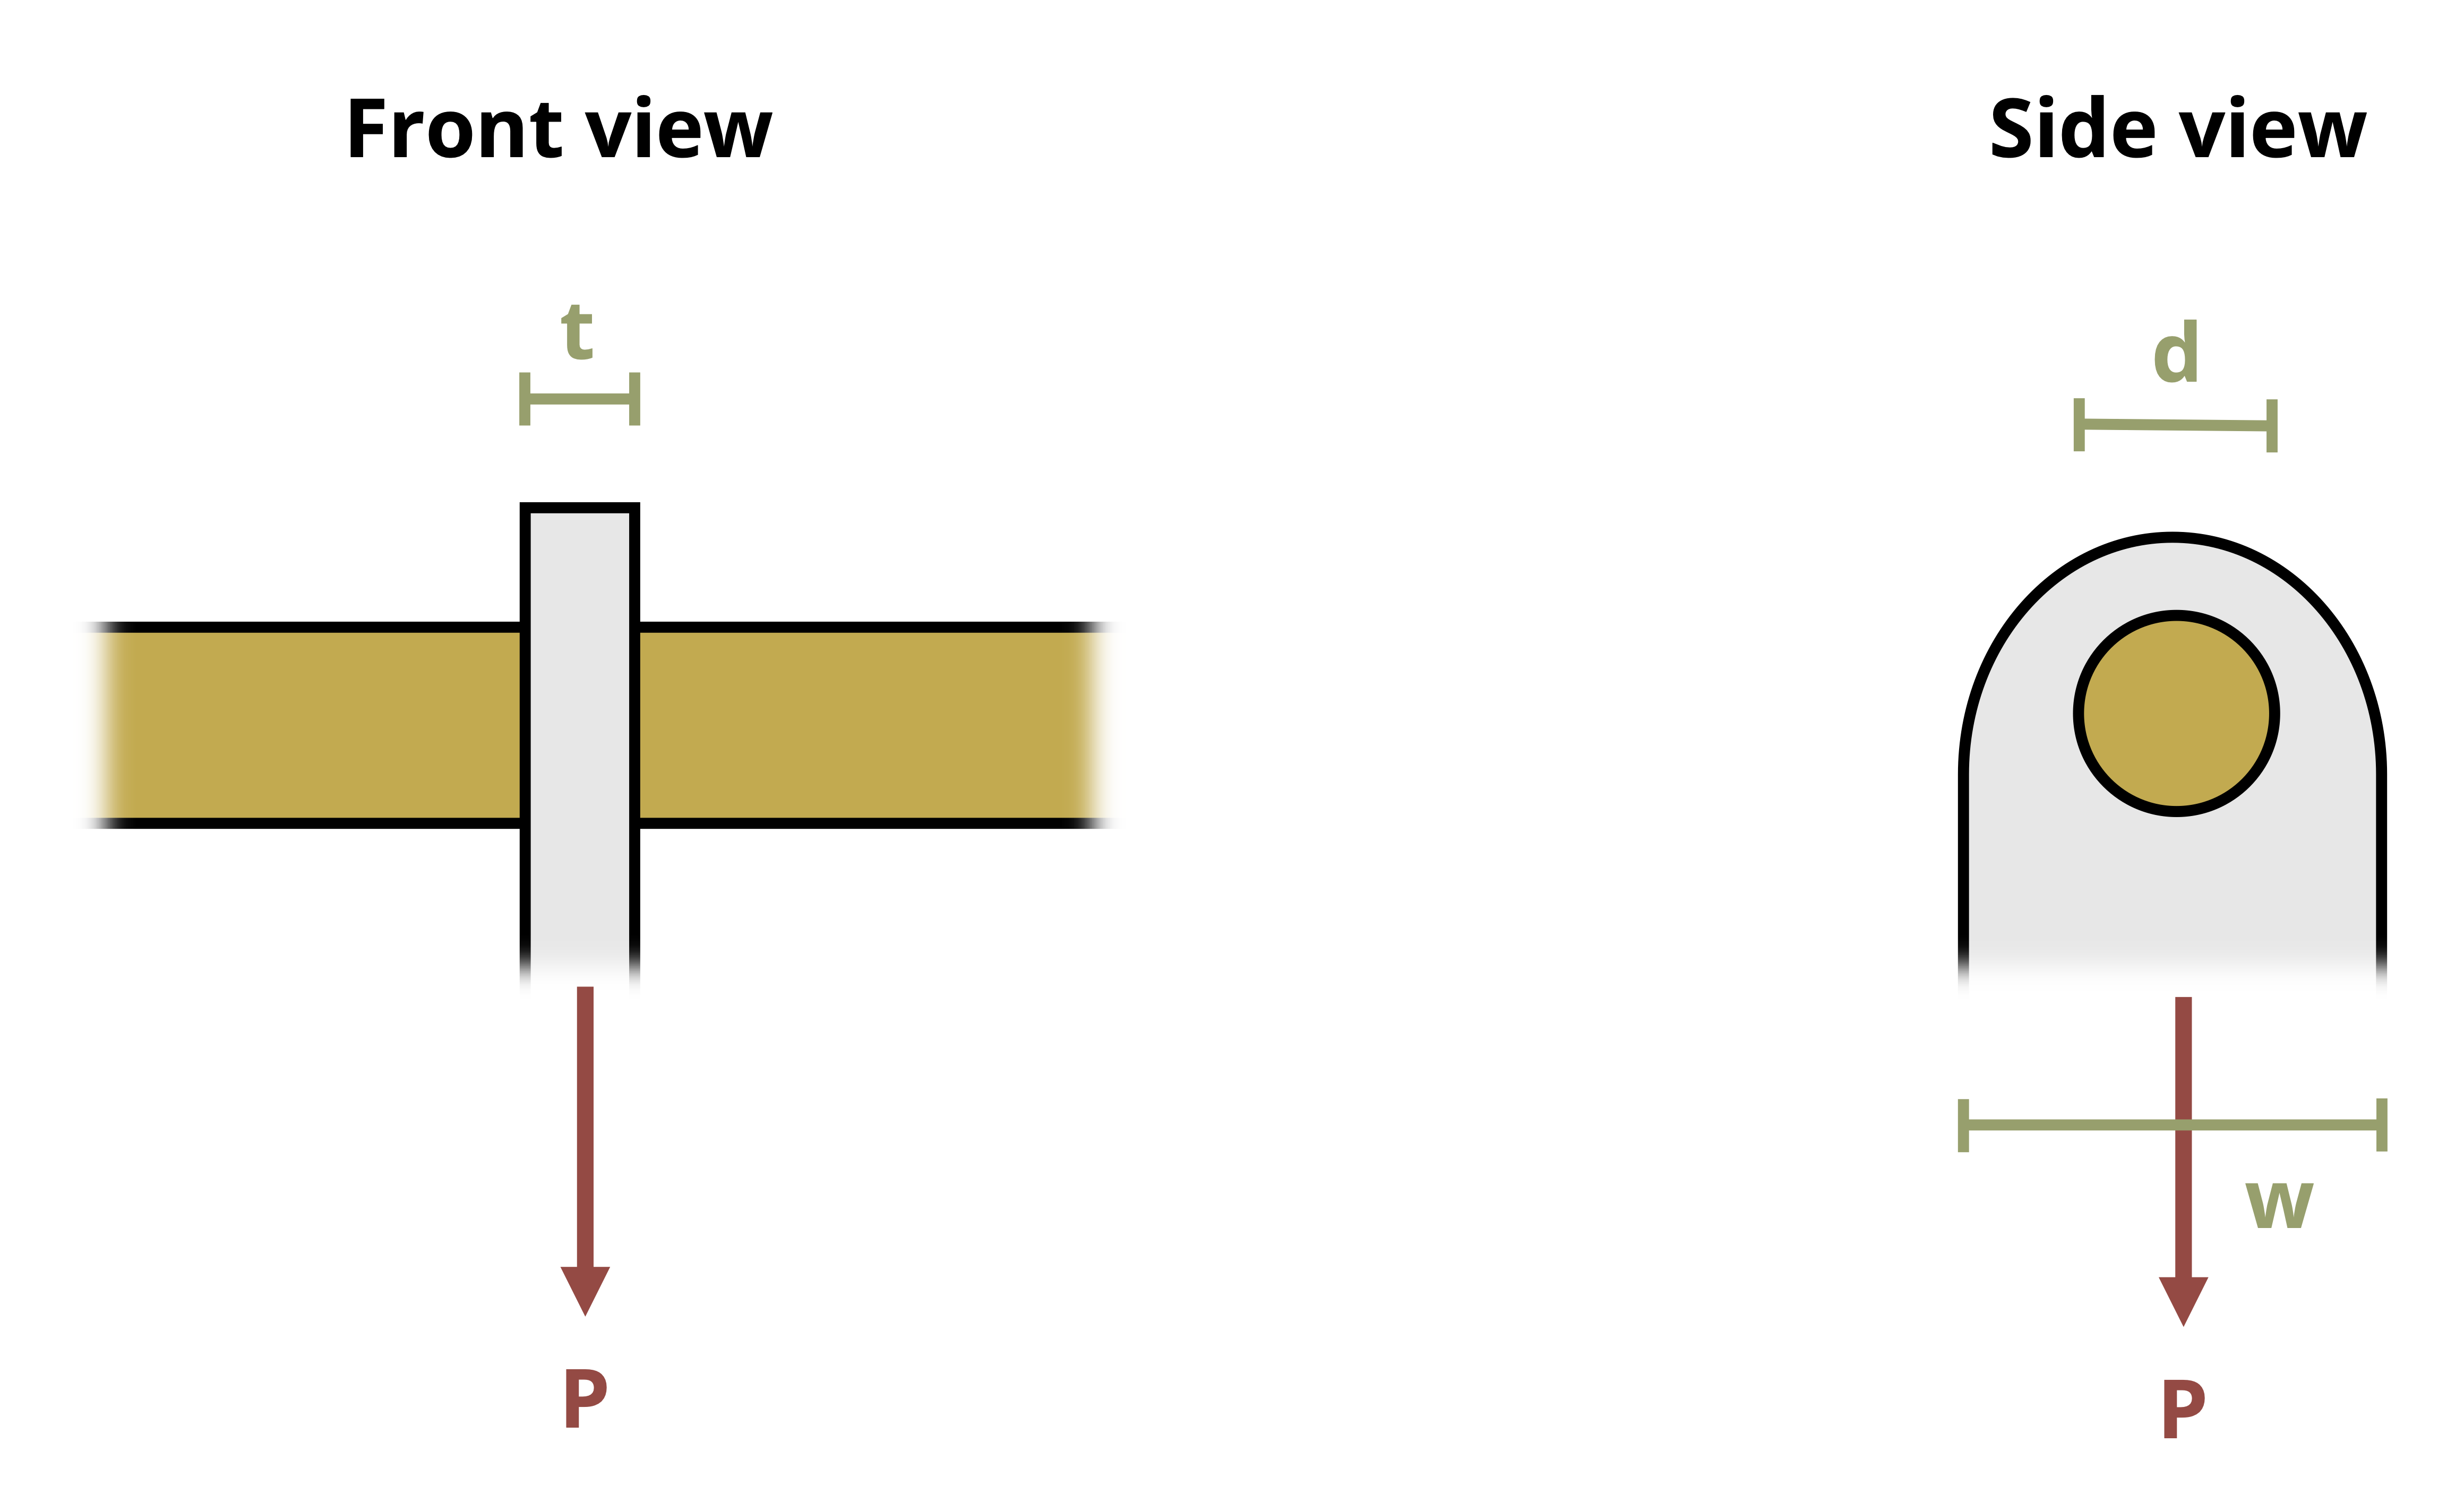
\includegraphics[keepaspectratio]{images/169.png}}
{[}Problem adapted from © Kurt Gramoll CC BY NC-SA 4.0{]}

\begin{Shaded}
\begin{Highlighting}[]
\NormalTok{\#| standalone: true}
\NormalTok{\#| viewerHeight: 600}
\NormalTok{\#| components: [viewer]}

\NormalTok{from shiny import App, render, ui, reactive}
\NormalTok{import random}
\NormalTok{import asyncio}
\NormalTok{import io}
\NormalTok{import math}
\NormalTok{import string}
\NormalTok{from datetime import datetime}
\NormalTok{from pathlib import Path}

\NormalTok{def generate\_random\_letters(length):}
\NormalTok{    \# Generate a random string of letters of specified length}
\NormalTok{    return \textquotesingle{}\textquotesingle{}.join(random.choice(string.ascii\_lowercase) for \_ in range(length))  }

\NormalTok{problem\_ID="169"}
\NormalTok{d=reactive.Value("\_\_")}
\NormalTok{t=reactive.Value("\_\_")}
\NormalTok{w=reactive.Value("\_\_")}
  
\NormalTok{attempts=["Timestamp,Attempt,Answer,Feedback\textbackslash{}n"]}

\NormalTok{app\_ui = ui.page\_fluid(}
\NormalTok{    ui.markdown("**Please enter your ID number from your instructor and click to generate your problem**"),}
\NormalTok{    ui.input\_text("ID","", placeholder="Enter ID Number Here"),}
\NormalTok{    ui.input\_action\_button("generate\_problem", "Generate Problem", class\_="btn{-}primary"),}
\NormalTok{    ui.markdown("**Problem Statement**"),}
\NormalTok{    ui.output\_ui("ui\_problem\_statement"),}
\NormalTok{    ui.input\_text("answer","Your Answer in units of kips", placeholder="Please enter your answer"),}
\NormalTok{    ui.input\_action\_button("submit", "Submit Answer", class\_="btn{-}primary"),}
\NormalTok{    ui.download\_button("download", "Download File to Submit", class\_="btn{-}success"),}
\NormalTok{)}

\NormalTok{def server(input, output, session):}
\NormalTok{    \# Initialize a counter for attempts}
\NormalTok{    attempt\_counter = reactive.Value(0)}

\NormalTok{    @output}
\NormalTok{    @render.ui}
\NormalTok{    def ui\_problem\_statement():}
\NormalTok{        return[ui.markdown(f"A steel connector plate is hung from a brass rod of diameter d = \{d()\} in. The plate has dimensions t = \{t()\} in. and w = \{w()\} in. Considering only bearing stress, find the minimum load (P) that will cause the connector or rod to fail. Assume the failure bearing stress for brass is 70 ksi and for steel is 75 ksi.")]}
    
\NormalTok{    @reactive.Effect}
\NormalTok{    @reactive.event(input.generate\_problem)}
\NormalTok{    def randomize\_vars():}
\NormalTok{        random.seed(input.ID())}
\NormalTok{        d.set(random.randrange(8, 20, 1)/10)}
\NormalTok{        t.set(random.randrange(3, 7, 1)/10)}
\NormalTok{        w.set((d()*2))        }

\NormalTok{    @reactive.Effect}
\NormalTok{    @reactive.event(input.submit)}
\NormalTok{    def \_():}
\NormalTok{        attempt\_counter.set(attempt\_counter() + 1)  \# Increment the attempt counter on each submission.}
\NormalTok{        instr= 70*t()*d()}
\NormalTok{        if math.isclose(float(input.answer()), instr, rel\_tol=0.01):}
\NormalTok{            check = "*Correct*"}
\NormalTok{            correct\_indicator = "JL"}
\NormalTok{        else:}
\NormalTok{            check = "*Not Correct.*"}
\NormalTok{            correct\_indicator = "JG"}

\NormalTok{        \# Generate random parts for the encoded attempt.}
\NormalTok{        random\_start = generate\_random\_letters(4)}
\NormalTok{        random\_middle = generate\_random\_letters(4)}
\NormalTok{        random\_end = generate\_random\_letters(4)}
\NormalTok{        encoded\_attempt = f"\{random\_start\}\{problem\_ID\}{-}\{random\_middle\}\{attempt\_counter()\}\{correct\_indicator\}{-}\{random\_end\}\{input.ID()\}"}

\NormalTok{        \# Store the most recent encoded attempt in a reactive value so it persists across submissions}
\NormalTok{        session.encoded\_attempt = reactive.Value(encoded\_attempt)}

\NormalTok{        \# Append the attempt data to the attempts list without the encoded attempt}
\NormalTok{        attempts.append(f"\{datetime.now()\}, \{attempt\_counter()\}, \{input.answer()\}, \{check\}\textbackslash{}n")}

\NormalTok{        \# Show feedback to the user.}
\NormalTok{        feedback = ui.markdown(f"Your answer of \{input.answer()\} is \{check\}.")}
\NormalTok{        m = ui.modal(}
\NormalTok{            feedback,}
\NormalTok{            title="Feedback",}
\NormalTok{            easy\_close=True}
\NormalTok{        )}
\NormalTok{        ui.modal\_show(m)}

\NormalTok{    @session.download(filename=lambda: f"Problem\_Log{-}\{problem\_ID\}{-}\{input.ID()\}.csv")}
\NormalTok{    async def download():}
\NormalTok{        \# Start the CSV with the encoded attempt (without label)}
\NormalTok{        final\_encoded = session.encoded\_attempt() if session.encoded\_attempt is not None else "No attempts"}
\NormalTok{        yield f"\{final\_encoded\}\textbackslash{}n\textbackslash{}n"}
        
\NormalTok{        \# Write the header for the remaining CSV data once}
\NormalTok{        yield "Timestamp,Attempt,Answer,Feedback\textbackslash{}n"}
        
\NormalTok{        \# Write the attempts data, ensure that the header from the attempts list is not written again}
\NormalTok{        for attempt in attempts[1:]:  \# Skip the first element which is the header}
\NormalTok{            await asyncio.sleep(0.25)  \# This delay may not be necessary; adjust as needed}
\NormalTok{            yield attempt}

\NormalTok{\# App installation}
\NormalTok{app = App(app\_ui, server)}
\end{Highlighting}
\end{Shaded}

\chapter*{Problem 2.47 - Stress on an Inclined
Plane}\label{problem-2.47---stress-on-an-inclined-plane}
\addcontentsline{toc}{chapter}{Problem 2.47 - Stress on an Inclined
Plane}

\markboth{Problem 2.47 - Stress on an Inclined Plane}{Problem 2.47 -
Stress on an Inclined Plane}

\pandocbounded{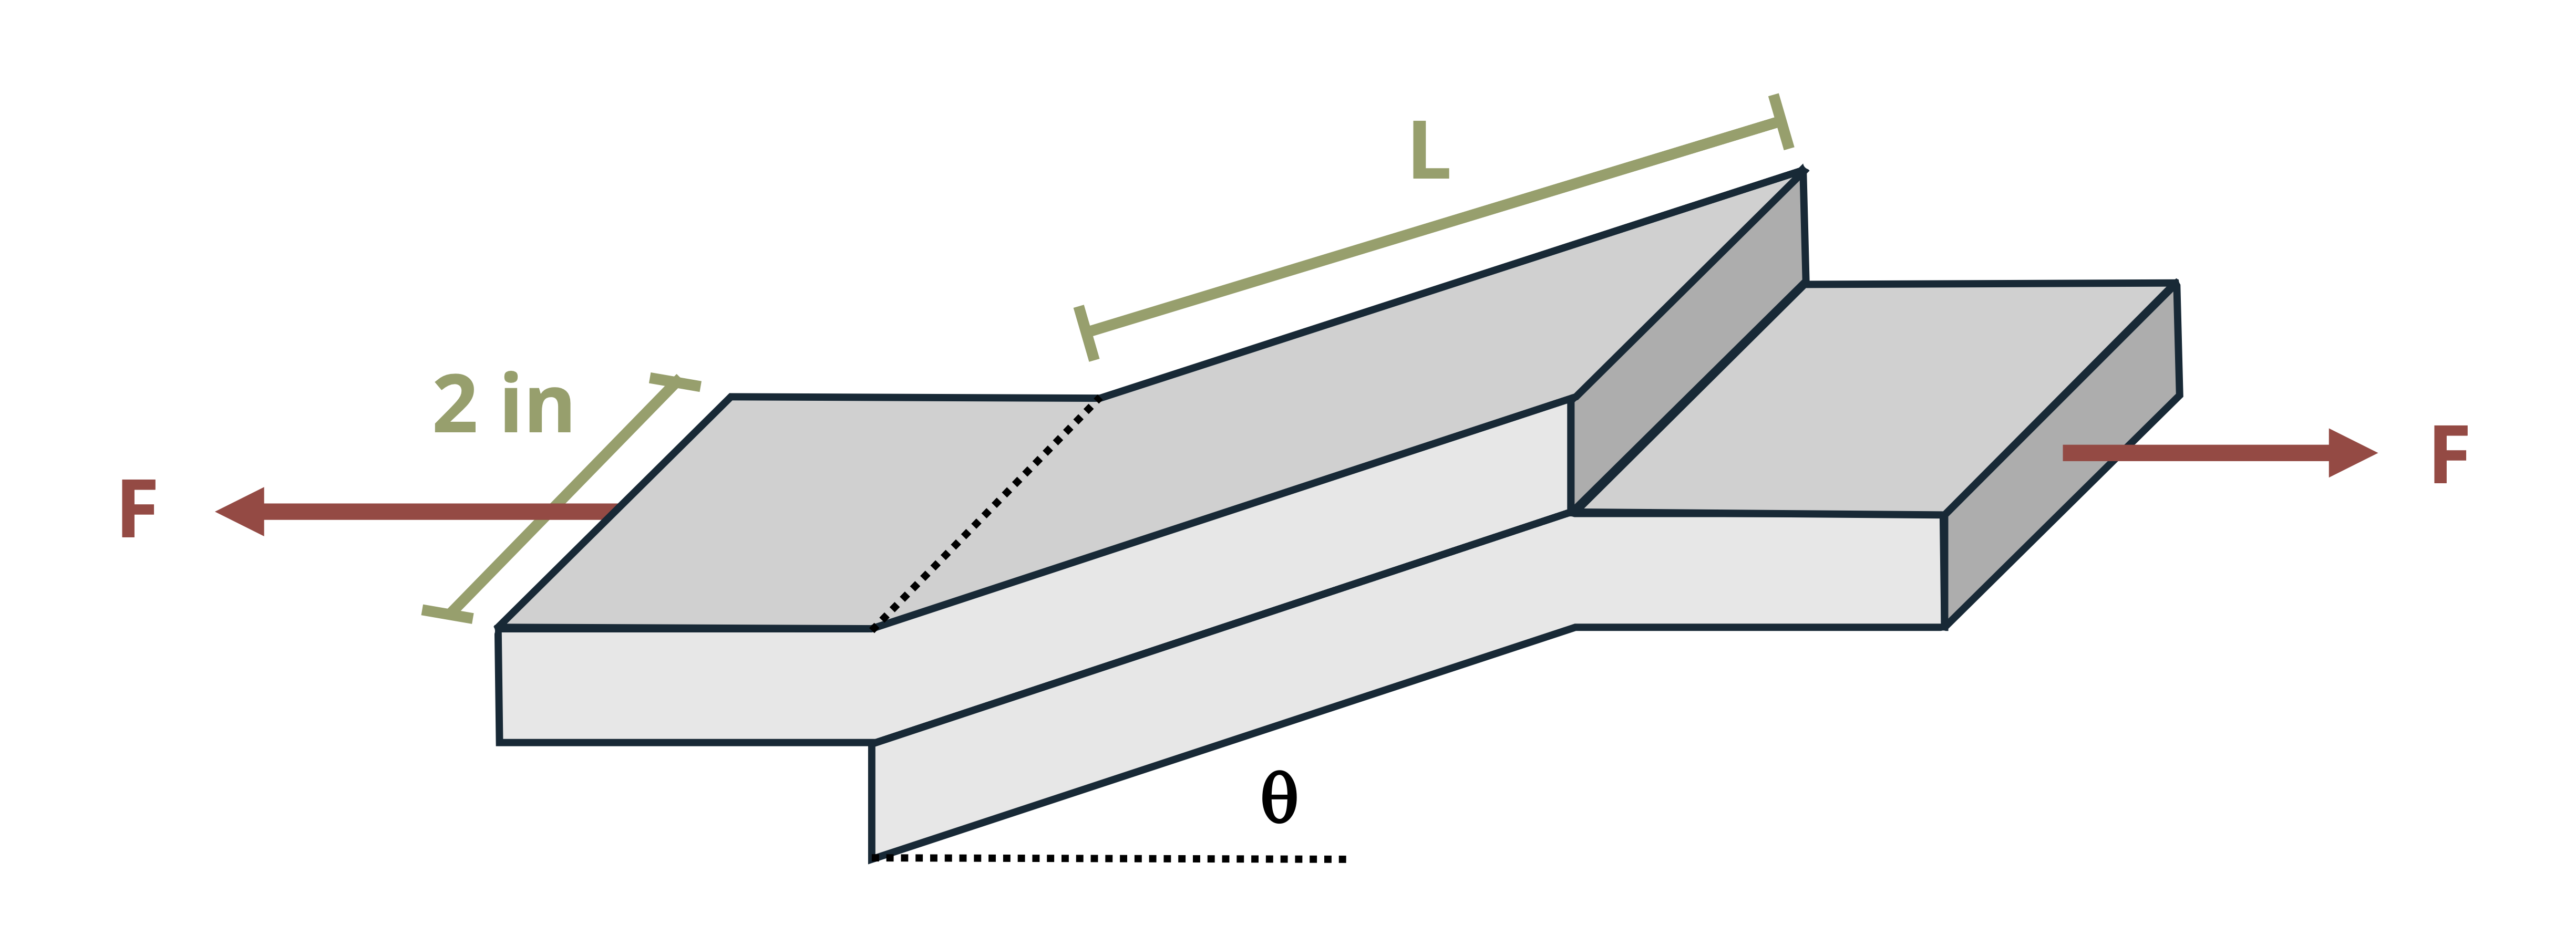
\includegraphics[keepaspectratio]{images/153.png}}
{[}Problem adapted from © Kurt Gramoll CC BY NC-SA 4.0{]}

\begin{Shaded}
\begin{Highlighting}[]
\NormalTok{\#| standalone: true}
\NormalTok{\#| viewerHeight: 600}
\NormalTok{\#| components: [viewer]}

\NormalTok{from shiny import App, render, ui, reactive}
\NormalTok{import random}
\NormalTok{import asyncio}
\NormalTok{import io}
\NormalTok{import math}
\NormalTok{import string}
\NormalTok{from datetime import datetime}
\NormalTok{from pathlib import Path}

\NormalTok{def generate\_random\_letters(length):}
\NormalTok{    \# Generate a random string of letters of specified length}
\NormalTok{    return \textquotesingle{}\textquotesingle{}.join(random.choice(string.ascii\_lowercase) for \_ in range(length))  }

\NormalTok{problem\_ID="153"}
\NormalTok{F=reactive.Value("\_\_")}
\NormalTok{L=reactive.Value("\_\_")}
\NormalTok{Θ=reactive.Value("\_\_")}

\NormalTok{attempts=["Timestamp,Attempt,Answer,Feedback\textbackslash{}n"]}

\NormalTok{app\_ui = ui.page\_fluid(}
\NormalTok{    ui.markdown("**Please enter your ID number from your instructor and click to generate your problem**"),}
\NormalTok{    ui.input\_text("ID","", placeholder="Enter ID Number Here"),}
\NormalTok{    ui.input\_action\_button("generate\_problem", "Generate Problem", class\_="btn{-}primary"),}
\NormalTok{    ui.markdown("**Problem Statement**"),}
\NormalTok{    ui.output\_ui("ui\_problem\_statement"),}
\NormalTok{    ui.input\_text("answer","Your Answer in units of psi", placeholder="Please enter your answer"),}
\NormalTok{    ui.input\_action\_button("submit", "Submit Answer", class\_="btn{-}primary"),}
\NormalTok{    ui.download\_button("download", "Download File to Submit", class\_="btn{-}success"),}
\NormalTok{)}

\NormalTok{def server(input, output, session):}
\NormalTok{    \# Initialize a counter for attempts}
\NormalTok{    attempt\_counter = reactive.Value(0)}

\NormalTok{    @output}
\NormalTok{    @render.ui}
\NormalTok{    def ui\_problem\_statement():}
\NormalTok{        return[ui.markdown(f"Two slanted brackets are glued together as shown. If F = \{F()\} lb, L = \{L()\} in., and Θ = \{Θ()\} °, determine the shear stress parallel to the inclined plane. Assume loads are inline and there is no rotation.")]}
    
\NormalTok{    @reactive.Effect}
\NormalTok{    @reactive.event(input.generate\_problem)}
\NormalTok{    def randomize\_vars():}
\NormalTok{        random.seed(input.ID())}
\NormalTok{        F.set(random.randrange(200, 800, 10))}
\NormalTok{        L.set(random.randrange(20, 80, 1)/10)}
\NormalTok{        Θ.set(random.randrange(15, 30, 1))}
        
\NormalTok{    @reactive.Effect}
\NormalTok{    @reactive.event(input.submit)}
\NormalTok{    def \_():}
\NormalTok{        attempt\_counter.set(attempt\_counter() + 1)  \# Increment the attempt counter on each submission.}
    
\NormalTok{        instr= (F()*math.cos(math.radians(Θ()))/(L()*2))}
\NormalTok{        if math.isclose(float(input.answer()), instr, rel\_tol=0.01):}
\NormalTok{            check = "*Correct*"}
\NormalTok{            correct\_indicator = "JL"}
\NormalTok{        else:}
\NormalTok{            check = "*Not Correct.*"}
\NormalTok{            correct\_indicator = "JG"}

\NormalTok{        \# Generate random parts for the encoded attempt.}
\NormalTok{        random\_start = generate\_random\_letters(4)}
\NormalTok{        random\_middle = generate\_random\_letters(4)}
\NormalTok{        random\_end = generate\_random\_letters(4)}
\NormalTok{        encoded\_attempt = f"\{random\_start\}\{problem\_ID\}{-}\{random\_middle\}\{attempt\_counter()\}\{correct\_indicator\}{-}\{random\_end\}\{input.ID()\}"}

\NormalTok{        \# Store the most recent encoded attempt in a reactive value so it persists across submissions}
\NormalTok{        session.encoded\_attempt = reactive.Value(encoded\_attempt)}

\NormalTok{        \# Append the attempt data to the attempts list without the encoded attempt}
\NormalTok{        attempts.append(f"\{datetime.now()\}, \{attempt\_counter()\}, \{input.answer()\}, \{check\}\textbackslash{}n")}

\NormalTok{        \# Show feedback to the user.}
\NormalTok{        feedback = ui.markdown(f"Your answer of \{input.answer()\} is \{check\}.")}
\NormalTok{        m = ui.modal(}
\NormalTok{            feedback,}
\NormalTok{            title="Feedback",}
\NormalTok{            easy\_close=True}
\NormalTok{        )}
\NormalTok{        ui.modal\_show(m)}

\NormalTok{    @session.download(filename=lambda: f"Problem\_Log{-}\{problem\_ID\}{-}\{input.ID()\}.csv")}
\NormalTok{    async def download():}
\NormalTok{        \# Start the CSV with the encoded attempt (without label)}
\NormalTok{        final\_encoded = session.encoded\_attempt() if session.encoded\_attempt is not None else "No attempts"}
\NormalTok{        yield f"\{final\_encoded\}\textbackslash{}n\textbackslash{}n"}
        
\NormalTok{        \# Write the header for the remaining CSV data once}
\NormalTok{        yield "Timestamp,Attempt,Answer,Feedback\textbackslash{}n"}
        
\NormalTok{        \# Write the attempts data, ensure that the header from the attempts list is not written again}
\NormalTok{        for attempt in attempts[1:]:  \# Skip the first element which is the header}
\NormalTok{            await asyncio.sleep(0.25)  \# This delay may not be necessary; adjust as needed}
\NormalTok{            yield attempt}

\NormalTok{\# App installation}
\NormalTok{app = App(app\_ui, server)}
\end{Highlighting}
\end{Shaded}

\chapter*{Problem 2.48 - Stress on an Inclined
Plane}\label{problem-2.48---stress-on-an-inclined-plane}
\addcontentsline{toc}{chapter}{Problem 2.48 - Stress on an Inclined
Plane}

\markboth{Problem 2.48 - Stress on an Inclined Plane}{Problem 2.48 -
Stress on an Inclined Plane}

\pandocbounded{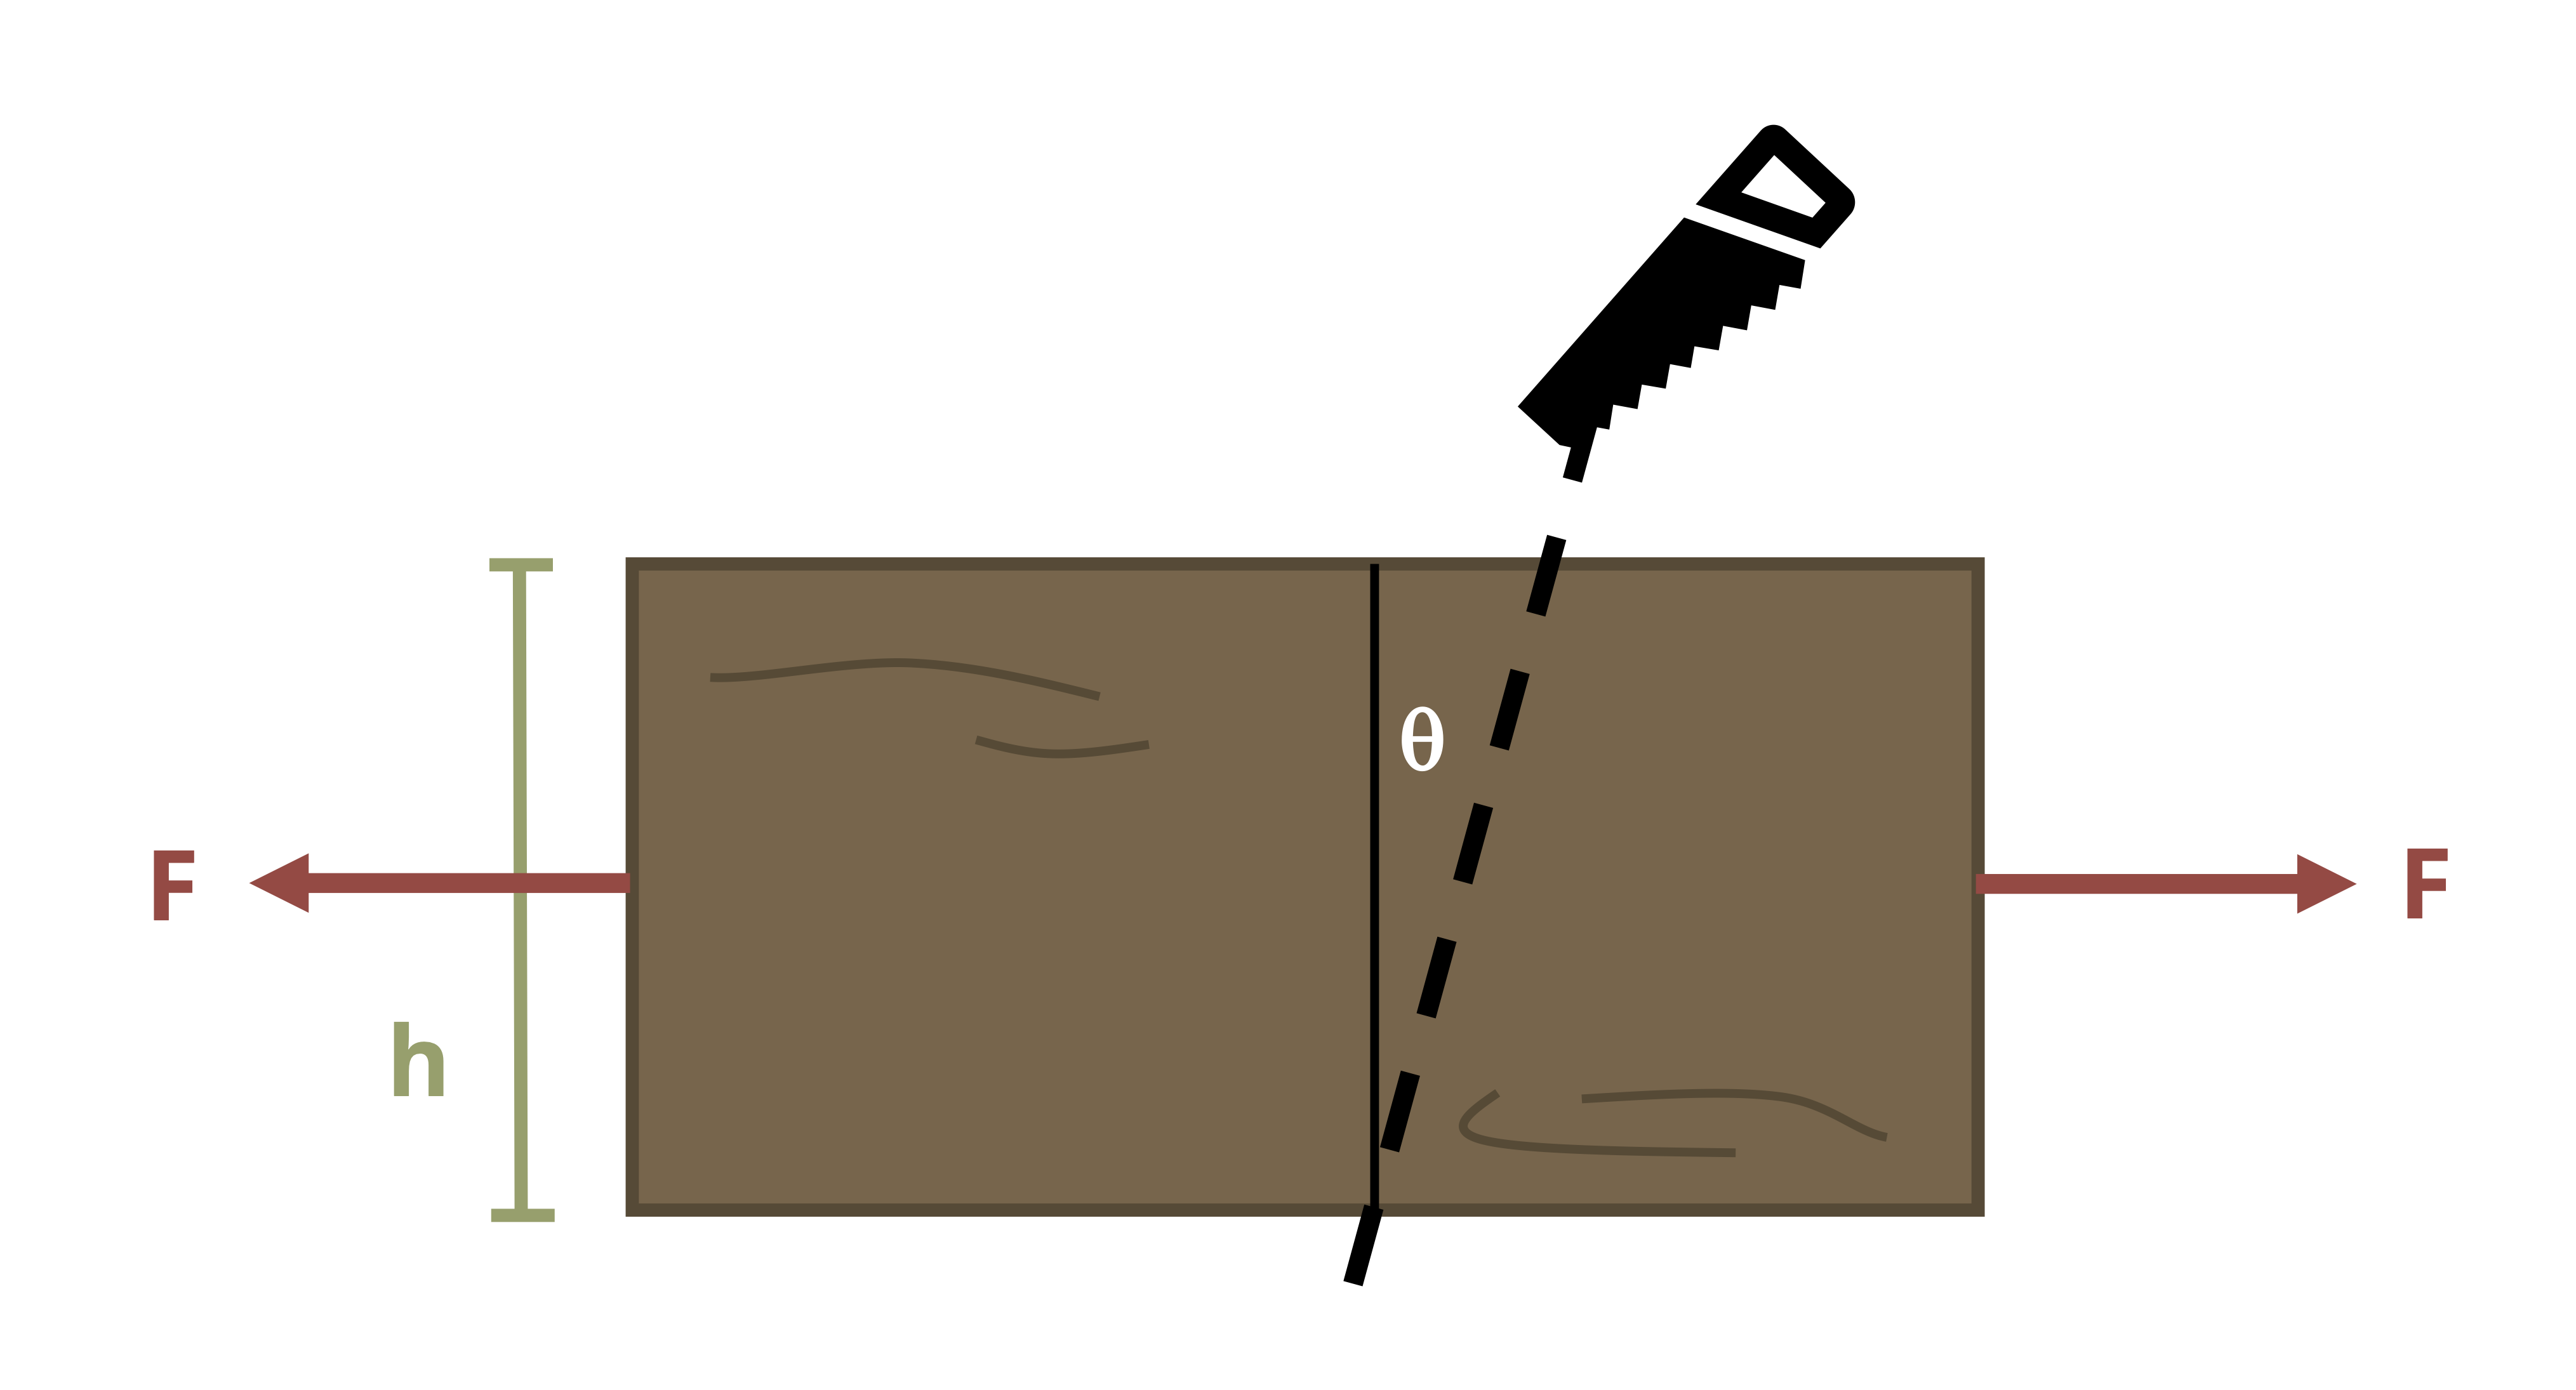
\includegraphics[keepaspectratio]{images/156.png}}
{[}Problem adapted from © Kurt Gramoll CC BY NC-SA 4.0{]}

\begin{Shaded}
\begin{Highlighting}[]
\NormalTok{\#| standalone: true}
\NormalTok{\#| viewerHeight: 600}
\NormalTok{\#| components: [viewer]}

\NormalTok{from shiny import App, render, ui, reactive}
\NormalTok{import random}
\NormalTok{import asyncio}
\NormalTok{import io}
\NormalTok{import math}
\NormalTok{import string}
\NormalTok{from datetime import datetime}
\NormalTok{from pathlib import Path}

\NormalTok{def generate\_random\_letters(length):}
\NormalTok{    \# Generate a random string of letters of specified length}
\NormalTok{    return \textquotesingle{}\textquotesingle{}.join(random.choice(string.ascii\_lowercase) for \_ in range(length))  }

\NormalTok{problem\_ID="156"}
\NormalTok{F=reactive.Value("\_\_")}
\NormalTok{h=reactive.Value("\_\_")}
\NormalTok{Θ=reactive.Value("\_\_")}

\NormalTok{attempts=["Timestamp,Attempt,Answer,Feedback\textbackslash{}n"]}

\NormalTok{app\_ui = ui.page\_fluid(}
\NormalTok{    ui.markdown("**Please enter your ID number from your instructor and click to generate your problem**"),}
\NormalTok{    ui.input\_text("ID","", placeholder="Enter ID Number Here"),}
\NormalTok{    ui.input\_action\_button("generate\_problem", "Generate Problem", class\_="btn{-}primary"),}
\NormalTok{    ui.markdown("**Problem Statement**"),}
\NormalTok{    ui.output\_ui("ui\_problem\_statement"),}
\NormalTok{    ui.input\_text("answer","Your Answer in units of psi", placeholder="Please enter your answer"),}
\NormalTok{    ui.input\_action\_button("submit", "Submit Answer", class\_="btn{-}primary"),}
\NormalTok{    ui.download\_button("download", "Download File to Submit", class\_="btn{-}success"),}
\NormalTok{)}


\NormalTok{def server(input, output, session):}
\NormalTok{    \# Initialize a counter for attempts}
\NormalTok{    attempt\_counter = reactive.Value(0)}

\NormalTok{    @output}
\NormalTok{    @render.ui}
\NormalTok{    def ui\_problem\_statement():}
\NormalTok{        return[ui.markdown(f"A 2 inch thick board is cut and then glued back together along a line that is Θ = \{Θ()\} ° off the vertical as shown. If height h = \{h()\} in. and F = \{F()\} lb, determine the normal stress along the cut line.")]}
    
\NormalTok{    @reactive.Effect}
\NormalTok{    @reactive.event(input.generate\_problem)}
\NormalTok{    def randomize\_vars():}
\NormalTok{        random.seed(input.ID())}
\NormalTok{        F.set(random.randrange(2000, 6000, 100))}
\NormalTok{        h.set(random.randrange(50, 150, 1)/10)}
\NormalTok{        Θ.set(random.randrange(10, 20, 1))}
        

\NormalTok{    @reactive.Effect}
\NormalTok{    @reactive.event(input.submit)}
\NormalTok{    def \_():}
\NormalTok{        attempt\_counter.set(attempt\_counter() + 1)  \# Increment the attempt counter on each submission.}
        
\NormalTok{        instr= (F()/(2*h()))*(math.cos(math.radians(Θ()))**2)}
\NormalTok{        if math.isclose(float(input.answer()), instr, rel\_tol=0.01):}
\NormalTok{            check = "*Correct*"}
\NormalTok{            correct\_indicator = "JL"}
\NormalTok{        else:}
\NormalTok{            check = "*Not Correct.*"}
\NormalTok{            correct\_indicator = "JG"}

\NormalTok{        \# Generate random parts for the encoded attempt.}
\NormalTok{        random\_start = generate\_random\_letters(4)}
\NormalTok{        random\_middle = generate\_random\_letters(4)}
\NormalTok{        random\_end = generate\_random\_letters(4)}
\NormalTok{        encoded\_attempt = f"\{random\_start\}\{problem\_ID\}{-}\{random\_middle\}\{attempt\_counter()\}\{correct\_indicator\}{-}\{random\_end\}\{input.ID()\}"}

\NormalTok{        \# Store the most recent encoded attempt in a reactive value so it persists across submissions}
\NormalTok{        session.encoded\_attempt = reactive.Value(encoded\_attempt)}

\NormalTok{        \# Append the attempt data to the attempts list without the encoded attempt}
\NormalTok{        attempts.append(f"\{datetime.now()\}, \{attempt\_counter()\}, \{input.answer()\}, \{check\}\textbackslash{}n")}

\NormalTok{        \# Show feedback to the user.}
\NormalTok{        feedback = ui.markdown(f"Your answer of \{input.answer()\} is \{check\}.")}
\NormalTok{        m = ui.modal(}
\NormalTok{            feedback,}
\NormalTok{            title="Feedback",}
\NormalTok{            easy\_close=True}
\NormalTok{        )}
\NormalTok{        ui.modal\_show(m)}

\NormalTok{    @session.download(filename=lambda: f"Problem\_Log{-}\{problem\_ID\}{-}\{input.ID()\}.csv")}
\NormalTok{    async def download():}
\NormalTok{        \# Start the CSV with the encoded attempt (without label)}
\NormalTok{        final\_encoded = session.encoded\_attempt() if session.encoded\_attempt is not None else "No attempts"}
\NormalTok{        yield f"\{final\_encoded\}\textbackslash{}n\textbackslash{}n"}
        
\NormalTok{        \# Write the header for the remaining CSV data once}
\NormalTok{        yield "Timestamp,Attempt,Answer,Feedback\textbackslash{}n"}
        
\NormalTok{        \# Write the attempts data, ensure that the header from the attempts list is not written again}
\NormalTok{        for attempt in attempts[1:]:  \# Skip the first element which is the header}
\NormalTok{            await asyncio.sleep(0.25)  \# This delay may not be necessary; adjust as needed}
\NormalTok{            yield attempt}


\NormalTok{\# App installation}
\NormalTok{app = App(app\_ui, server)}
\end{Highlighting}
\end{Shaded}

\part{Chapter 3 Problems}

\chapter*{Problem 3.2 - Normal
Strain}\label{problem-3.2---normal-strain}
\addcontentsline{toc}{chapter}{Problem 3.2 - Normal Strain}

\markboth{Problem 3.2 - Normal Strain}{Problem 3.2 - Normal Strain}

\begin{figure}[H]

{\centering 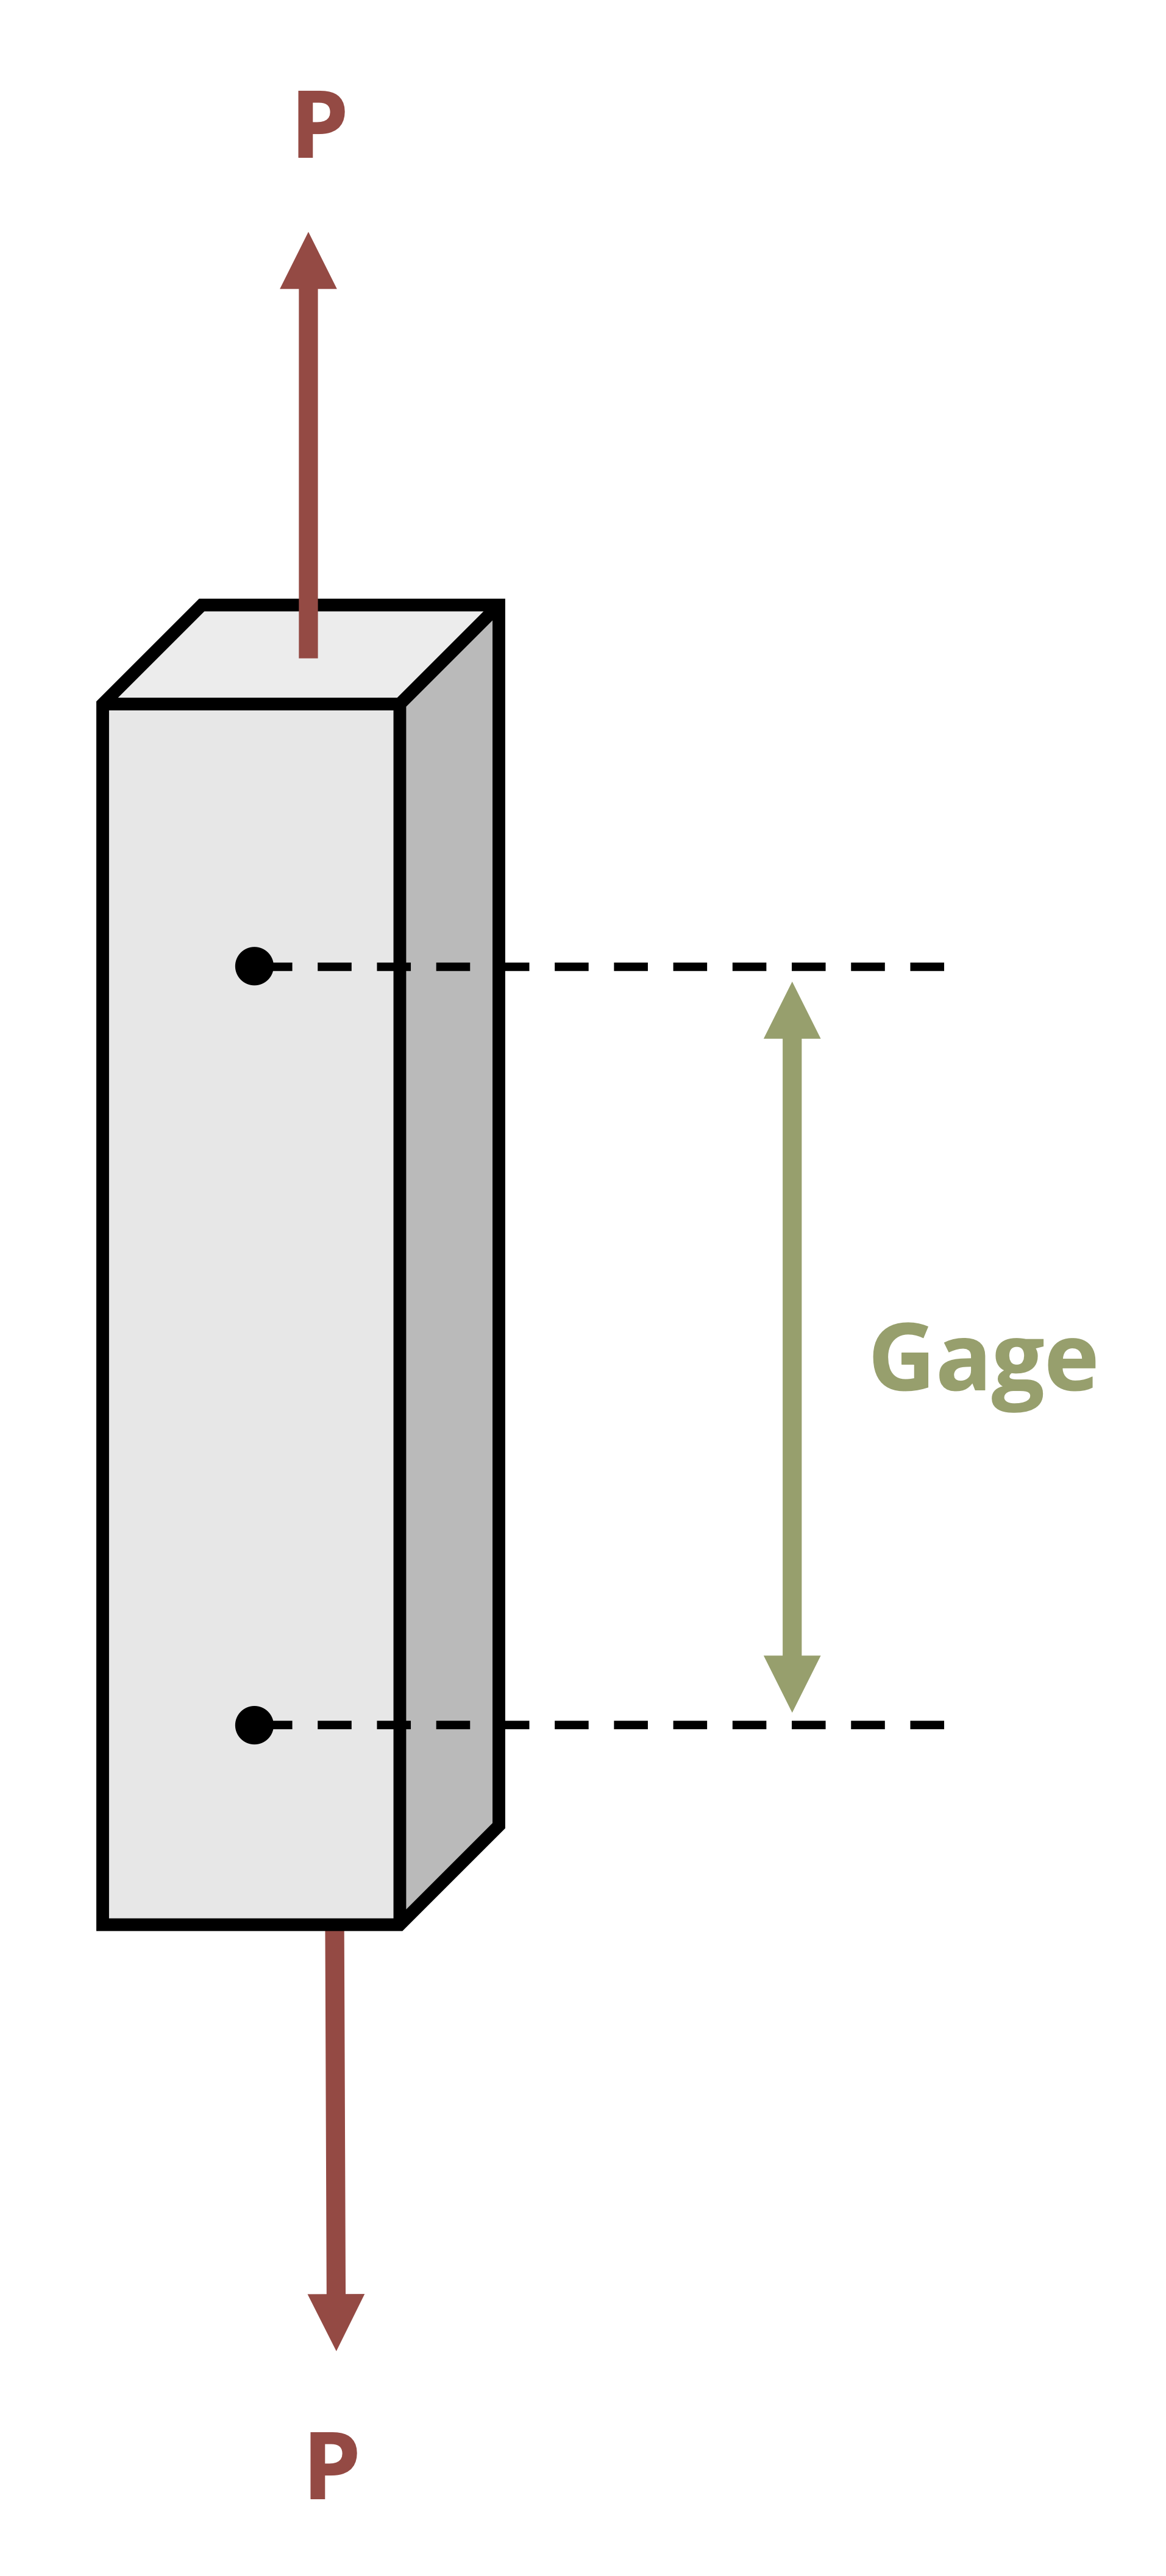
\includegraphics[width=1.5625in,height=\textheight,keepaspectratio]{images/650.png}

}

\caption{Figure 1: A rectangular prism is subjected to a tension test.}

\end{figure}%

{[}Problem adapted from © Chris Galitz CC BY NC-SA 4.0{]}

\begin{Shaded}
\begin{Highlighting}[]
\NormalTok{\#| standalone: true}
\NormalTok{\#| viewerHeight: 600}
\NormalTok{\#| components: [viewer]}

\NormalTok{from shiny import App, render, ui, reactive}
\NormalTok{import random}
\NormalTok{import asyncio}
\NormalTok{import io}
\NormalTok{import math}
\NormalTok{import string}
\NormalTok{from datetime import datetime}
\NormalTok{from pathlib import Path}

\NormalTok{def generate\_random\_letters(length):}
\NormalTok{    \# Generate a random string of letters of specified length}
\NormalTok{    return \textquotesingle{}\textquotesingle{}.join(random.choice(string.ascii\_lowercase) for \_ in range(length))  }

\NormalTok{problem\_ID="650"}
\NormalTok{L=reactive.Value("\_\_")}
\NormalTok{Lp=reactive.Value("\_\_")}

  
\NormalTok{attempts=["Timestamp,Attempt,Answer,Feedback\textbackslash{}n"]}

\NormalTok{app\_ui = ui.page\_fluid(}
\NormalTok{    ui.markdown("**Please enter your ID number from your instructor and click to generate your problem**"),}
\NormalTok{    ui.input\_text("ID","", placeholder="Enter ID Number Here"),}
\NormalTok{    ui.input\_action\_button("generate\_problem", "Generate Problem", class\_="btn{-}primary"),}
\NormalTok{    ui.markdown("**Problem Statement**"),}
\NormalTok{    ui.output\_ui("ui\_problem\_statement"),}
\NormalTok{    ui.input\_text("answer","Your Answer in units of mm/mm", placeholder="Please enter your answer"),}
\NormalTok{    ui.input\_action\_button("submit", "Submit Answer", class\_="btn{-}primary"),}
\NormalTok{    ui.download\_button("download", "Download File to Submit", class\_="btn{-}success"),}
\NormalTok{)}


\NormalTok{def server(input, output, session):}
\NormalTok{    \# Initialize a counter for attempts}
\NormalTok{    attempt\_counter = reactive.Value(0)}

\NormalTok{    @output}
\NormalTok{    @render.ui}
\NormalTok{    def ui\_problem\_statement():}
\NormalTok{        return[ui.markdown(f"During a tension test of a rectangular prism, the original gage length L = \{L()\} mm is increased to L\textquotesingle{} = \{Lp()\} mm. determine the normal strain, ε, in the prism.")]}
    
\NormalTok{    @reactive.Effect}
\NormalTok{    @reactive.event(input.generate\_problem)}
\NormalTok{    def randomize\_vars():}
\NormalTok{        random.seed(input.ID())}
\NormalTok{        L.set(random.randrange(100, 400, 1))}
\NormalTok{        Lp.set(L()+random.randrange(100, 300, 1)/100)}
        
\NormalTok{    @reactive.Effect}
\NormalTok{    @reactive.event(input.submit)}
\NormalTok{    def \_():}
\NormalTok{        attempt\_counter.set(attempt\_counter() + 1)  \# Increment the attempt counter on each submission.}
\NormalTok{        instr= (Lp(){-}L())/L()}
\NormalTok{        if math.isclose(float(input.answer()), instr, rel\_tol=0.01):}
\NormalTok{            check = "*Correct*"}
\NormalTok{            correct\_indicator = "JL"}
\NormalTok{        else:}
\NormalTok{            check = "*Not Correct.*"}
\NormalTok{            correct\_indicator = "JG"}

\NormalTok{        \# Generate random parts for the encoded attempt.}
\NormalTok{        random\_start = generate\_random\_letters(4)}
\NormalTok{        random\_middle = generate\_random\_letters(4)}
\NormalTok{        random\_end = generate\_random\_letters(4)}
\NormalTok{        encoded\_attempt = f"\{random\_start\}\{problem\_ID\}{-}\{random\_middle\}\{attempt\_counter()\}\{correct\_indicator\}{-}\{random\_end\}\{input.ID()\}"}

\NormalTok{        \# Store the most recent encoded attempt in a reactive value so it persists across submissions}
\NormalTok{        session.encoded\_attempt = reactive.Value(encoded\_attempt)}

\NormalTok{        \# Append the attempt data to the attempts list without the encoded attempt}
\NormalTok{        attempts.append(f"\{datetime.now()\}, \{attempt\_counter()\}, \{input.answer()\}, \{check\}\textbackslash{}n")}

\NormalTok{        \# Show feedback to the user.}
\NormalTok{        feedback = ui.markdown(f"Your answer of \{input.answer()\} is \{check\}.")}
\NormalTok{        m = ui.modal(}
\NormalTok{            feedback,}
\NormalTok{            title="Feedback",}
\NormalTok{            easy\_close=True}
\NormalTok{        )}
\NormalTok{        ui.modal\_show(m)}

\NormalTok{    @session.download(filename=lambda: f"Problem\_Log{-}\{problem\_ID\}{-}\{input.ID()\}.csv")}
\NormalTok{    async def download():}
\NormalTok{        \# Start the CSV with the encoded attempt (without label)}
\NormalTok{        final\_encoded = session.encoded\_attempt() if session.encoded\_attempt is not None else "No attempts"}
\NormalTok{        yield f"\{final\_encoded\}\textbackslash{}n\textbackslash{}n"}
        
\NormalTok{        \# Write the header for the remaining CSV data once}
\NormalTok{        yield "Timestamp,Attempt,Answer,Feedback\textbackslash{}n"}
        
\NormalTok{        \# Write the attempts data, ensure that the header from the attempts list is not written again}
\NormalTok{        for attempt in attempts[1:]:  \# Skip the first element which is the header}
\NormalTok{            await asyncio.sleep(0.25)  \# This delay may not be necessary; adjust as needed}
\NormalTok{            yield attempt}


\NormalTok{\# App installation}
\NormalTok{app = App(app\_ui, server)}
\end{Highlighting}
\end{Shaded}

\chapter*{Problem 3.7 - Shear Strain}\label{problem-3.7---shear-strain}
\addcontentsline{toc}{chapter}{Problem 3.7 - Shear Strain}

\markboth{Problem 3.7 - Shear Strain}{Problem 3.7 - Shear Strain}

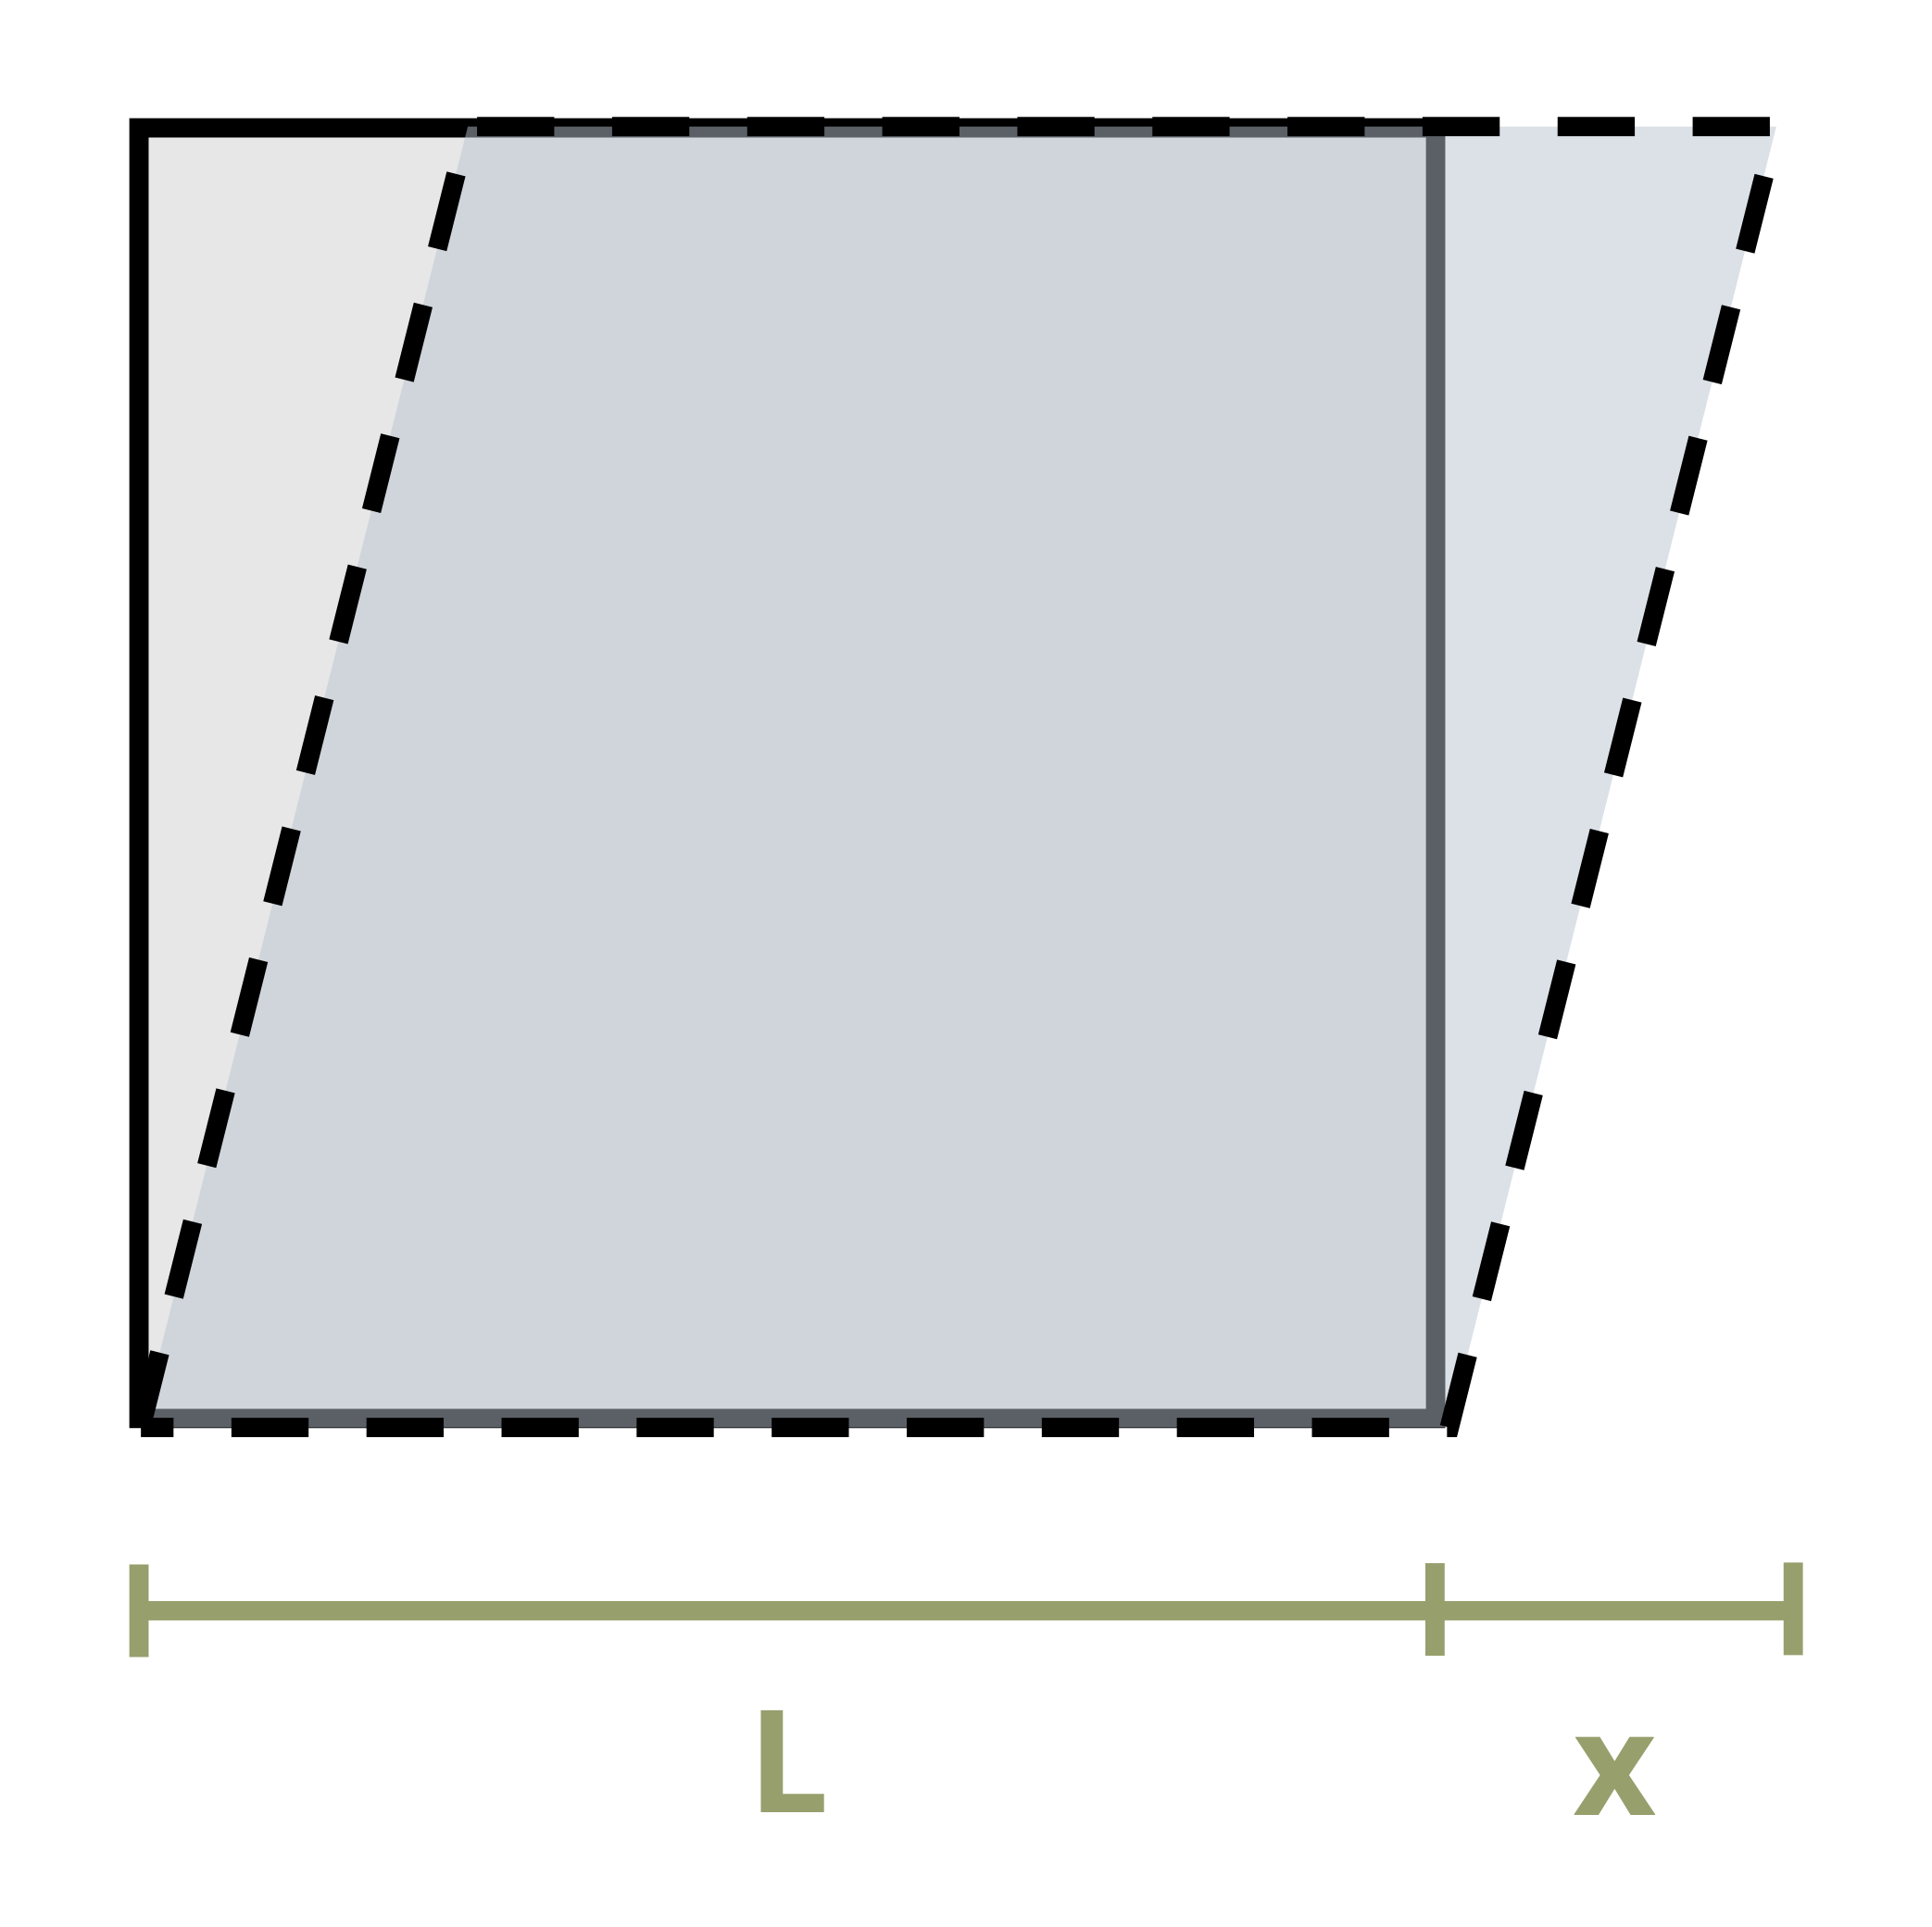
\includegraphics[width=3.125in,height=\textheight,keepaspectratio]{images/652.png}
{[}Problem adapted from © Chris Galitz CC BY NC-SA 4.0{]}

\begin{Shaded}
\begin{Highlighting}[]
\NormalTok{\#| standalone: true}
\NormalTok{\#| viewerHeight: 600}
\NormalTok{\#| components: [viewer]}

\NormalTok{from shiny import App, render, ui, reactive}
\NormalTok{import random}
\NormalTok{import asyncio}
\NormalTok{import io}
\NormalTok{import math}
\NormalTok{import string}
\NormalTok{from datetime import datetime}
\NormalTok{from pathlib import Path}

\NormalTok{def generate\_random\_letters(length):}
\NormalTok{    \# Generate a random string of letters of specified length}
\NormalTok{    return \textquotesingle{}\textquotesingle{}.join(random.choice(string.ascii\_lowercase) for \_ in range(length))  }

\NormalTok{problem\_ID="652"}
\NormalTok{L=reactive.Value("\_\_")}
\NormalTok{x=reactive.Value("\_\_")}

  
\NormalTok{attempts=["Timestamp,Attempt,Answer,Feedback\textbackslash{}n"]}

\NormalTok{app\_ui = ui.page\_fluid(}
\NormalTok{    ui.markdown("**Please enter your ID number from your instructor and click to generate your problem**"),}
\NormalTok{    ui.input\_text("ID","", placeholder="Enter ID Number Here"),}
\NormalTok{    ui.input\_action\_button("generate\_problem", "Generate Problem", class\_="btn{-}primary"),}
\NormalTok{    ui.markdown("**Problem Statement**"),}
\NormalTok{    ui.output\_ui("ui\_problem\_statement"),}
\NormalTok{    ui.input\_text("answer","Your Answer in units of radians", placeholder="Please enter your answer"),}
\NormalTok{    ui.input\_action\_button("submit", "Submit Answer", class\_="btn{-}primary"),}
\NormalTok{    ui.download\_button("download", "Download File to Submit", class\_="btn{-}success"),}
\NormalTok{)}


\NormalTok{def server(input, output, session):}
\NormalTok{    \# Initialize a counter for attempts}
\NormalTok{    attempt\_counter = reactive.Value(0)}

\NormalTok{    @output}
\NormalTok{    @render.ui}
\NormalTok{    def ui\_problem\_statement():}
\NormalTok{        return[ui.markdown(f"A square plate is deformed due to shear with the new shape shown. If length L = \{L()\} mm and x = \{x()\} mm, determine the shear strain at corner A.")]}
    
\NormalTok{    @reactive.Effect}
\NormalTok{    @reactive.event(input.generate\_problem)}
\NormalTok{    def randomize\_vars():}
\NormalTok{        random.seed(input.ID())}
\NormalTok{        L.set(random.randrange(200, 500, 10))}
\NormalTok{        x.set(random.randrange(20, 50, 1))}
        
\NormalTok{    @reactive.Effect}
\NormalTok{    @reactive.event(input.submit)}
\NormalTok{    def \_():}
\NormalTok{        attempt\_counter.set(attempt\_counter() + 1)  \# Increment the attempt counter on each submission.}
\NormalTok{        instr= math.atan(x()/L())}
\NormalTok{        if math.isclose(float(input.answer()), instr, rel\_tol=0.01):}
\NormalTok{            check = "*Correct*"}
\NormalTok{            correct\_indicator = "JL"}
\NormalTok{        else:}
\NormalTok{            check = "*Not Correct.*"}
\NormalTok{            correct\_indicator = "JG"}

\NormalTok{        \# Generate random parts for the encoded attempt.}
\NormalTok{        random\_start = generate\_random\_letters(4)}
\NormalTok{        random\_middle = generate\_random\_letters(4)}
\NormalTok{        random\_end = generate\_random\_letters(4)}
\NormalTok{        encoded\_attempt = f"\{random\_start\}\{problem\_ID\}{-}\{random\_middle\}\{attempt\_counter()\}\{correct\_indicator\}{-}\{random\_end\}\{input.ID()\}"}

\NormalTok{        \# Store the most recent encoded attempt in a reactive value so it persists across submissions}
\NormalTok{        session.encoded\_attempt = reactive.Value(encoded\_attempt)}

\NormalTok{        \# Append the attempt data to the attempts list without the encoded attempt}
\NormalTok{        attempts.append(f"\{datetime.now()\}, \{attempt\_counter()\}, \{input.answer()\}, \{check\}\textbackslash{}n")}

\NormalTok{        \# Show feedback to the user.}
\NormalTok{        feedback = ui.markdown(f"Your answer of \{input.answer()\} is \{check\}.")}
\NormalTok{        m = ui.modal(}
\NormalTok{            feedback,}
\NormalTok{            title="Feedback",}
\NormalTok{            easy\_close=True}
\NormalTok{        )}
\NormalTok{        ui.modal\_show(m)}

\NormalTok{    @session.download(filename=lambda: f"Problem\_Log{-}\{problem\_ID\}{-}\{input.ID()\}.csv")}
\NormalTok{    async def download():}
\NormalTok{        \# Start the CSV with the encoded attempt (without label)}
\NormalTok{        final\_encoded = session.encoded\_attempt() if session.encoded\_attempt is not None else "No attempts"}
\NormalTok{        yield f"\{final\_encoded\}\textbackslash{}n\textbackslash{}n"}
        
\NormalTok{        \# Write the header for the remaining CSV data once}
\NormalTok{        yield "Timestamp,Attempt,Answer,Feedback\textbackslash{}n"}
        
\NormalTok{        \# Write the attempts data, ensure that the header from the attempts list is not written again}
\NormalTok{        for attempt in attempts[1:]:  \# Skip the first element which is the header}
\NormalTok{            await asyncio.sleep(0.25)  \# This delay may not be necessary; adjust as needed}
\NormalTok{            yield attempt}


\NormalTok{\# App installation}
\NormalTok{app = App(app\_ui, server)}
\end{Highlighting}
\end{Shaded}

\part{Chapter 4 Problems}

\chapter*{Problem 4.5 - Hooke's Law}\label{problem-4.5---hookes-law}
\addcontentsline{toc}{chapter}{Problem 4.5 - Hooke's Law}

\markboth{Problem 4.5 - Hooke's Law}{Problem 4.5 - Hooke's Law}

\begin{figure}[H]

{\centering \pandocbounded{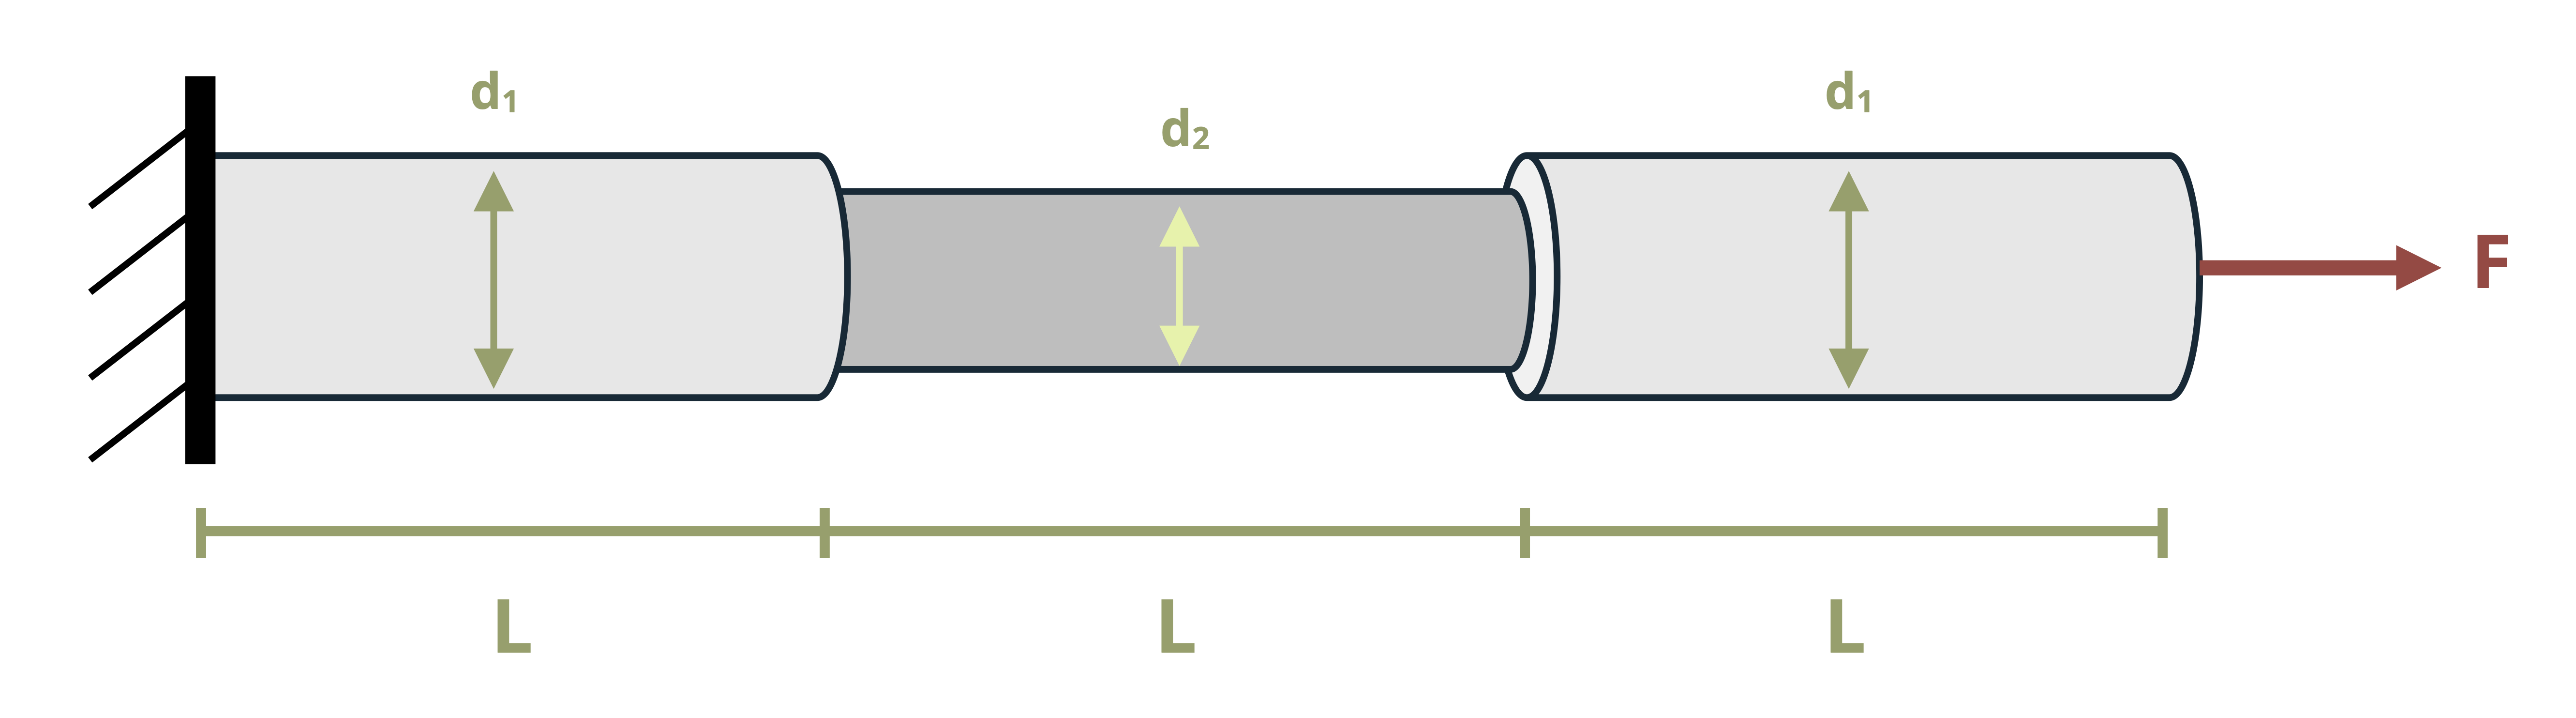
\includegraphics[keepaspectratio]{images/188.png}}

}

\caption{Figure 1: A single force pulls on three cylindrical rods that
are fixed to a wall.}

\end{figure}%

{[}Problem adapted from © Kurt Gramoll CC BY NC-SA 4.0{]}

\begin{Shaded}
\begin{Highlighting}[]
\NormalTok{\#| standalone: true}
\NormalTok{\#| viewerHeight: 600}
\NormalTok{\#| components: [viewer]}

\NormalTok{from shiny import App, render, ui, reactive}
\NormalTok{import random}
\NormalTok{import asyncio}
\NormalTok{import io}
\NormalTok{import math}
\NormalTok{import string}
\NormalTok{from datetime import datetime}
\NormalTok{from pathlib import Path}

\NormalTok{def generate\_random\_letters(length):}
\NormalTok{    \# Generate a random string of letters of specified length}
\NormalTok{    return \textquotesingle{}\textquotesingle{}.join(random.choice(string.ascii\_lowercase) for \_ in range(length))}

\NormalTok{problem\_ID="188"}
\NormalTok{F=reactive.Value("\_\_")}
\NormalTok{L=reactive.Value("\_\_")}
\NormalTok{d1=reactive.Value("\_\_")}
\NormalTok{d2=reactive.Value("\_\_")}
\NormalTok{Esteel = 29000}
\NormalTok{Ealuminum = 10000}


\NormalTok{attempts=["Timestamp,Attempt,Answer,Feedback\textbackslash{}n"]}

\NormalTok{app\_ui = ui.page\_fluid(}
\NormalTok{    ui.markdown("**Please enter your ID number from your instructor and click to generate your problem**"),}
\NormalTok{    ui.input\_text("ID","", placeholder="Enter ID Number Here"),}
\NormalTok{    ui.input\_action\_button("generate\_problem", "Generate Problem", class\_="btn{-}primary"),}
\NormalTok{    ui.markdown("**Problem Statement**"),}
\NormalTok{    ui.output\_ui("ui\_problem\_statement"),}
\NormalTok{    ui.input\_text("answer","Your Answer in units of inches/inches", placeholder="Please enter your answer"),}
\NormalTok{    ui.input\_action\_button("submit", "Submit Answer", class\_="btn{-}primary"),}
\NormalTok{    ui.download\_button("download", "Download File to Submit", class\_="btn{-}success"),}
\NormalTok{)}


\NormalTok{def server(input, output, session):}
\NormalTok{    \# Initialize a counter for attempts}
\NormalTok{    attempt\_counter = reactive.Value(0)}

\NormalTok{    @output}
\NormalTok{    @render.ui}
\NormalTok{    def ui\_problem\_statement():}
\NormalTok{        return[ui.markdown(f"A single force F = \{F()\} kips pulls on three cylindrical rods, each of length L = \{L()\} in. The aluminum rods have a diameter d\textless{}sub\textgreater{}1\textless{}/sub\textgreater{} = \{d1()\} in., and the steel rods have a diameter d\textless{}sub\textgreater{}2\textless{}/sub\textgreater{} = \{d2()\} in. What is the strain in the steel cylinder? Assume E\textless{}sub\textgreater{}steel\textless{}/sub\textgreater{} = 29,000 ksi and E\textless{}sub\textgreater{}aluminum\textless{}/sub\textgreater{} = 10,000 ksi.")]}
    
\NormalTok{    @reactive.Effect}
\NormalTok{    @reactive.event(input.generate\_problem)}
\NormalTok{    def randomize\_vars():}
\NormalTok{        random.seed(input.ID())}
\NormalTok{        F.set(random.randrange(20, 300, 1)/10)}
\NormalTok{        L.set(random.randrange(50, 200, 1)/10)}
\NormalTok{        d1.set(random.randrange(10, 50, 1)/10)}
\NormalTok{        d2.set(round(d1()/2, 2))}
        
\NormalTok{    @reactive.Effect}
\NormalTok{    @reactive.event(input.submit)}
\NormalTok{    def \_():}
\NormalTok{        attempt\_counter.set(attempt\_counter() + 1)  \# Increment the attempt counter on each submission.}
\NormalTok{        instr=(F()/(((d2()/2)**2)*math.pi))/Esteel}
\NormalTok{        if math.isclose(float(input.answer()), instr, rel\_tol=0.01):}
\NormalTok{            check = "*Correct*"}
\NormalTok{            correct\_indicator = "JL"}
\NormalTok{        else:}
\NormalTok{            check = "*Not Correct.*"}
\NormalTok{            correct\_indicator = "JG"}

\NormalTok{        \# Generate random parts for the encoded attempt.}
\NormalTok{        random\_start = generate\_random\_letters(4)}
\NormalTok{        random\_middle = generate\_random\_letters(4)}
\NormalTok{        random\_end = generate\_random\_letters(4)}
\NormalTok{        encoded\_attempt = f"\{random\_start\}\{problem\_ID\}{-}\{random\_middle\}\{attempt\_counter()\}\{correct\_indicator\}{-}\{random\_end\}\{input.ID()\}"}

\NormalTok{        \# Store the most recent encoded attempt in a reactive value so it persists across submissions}
\NormalTok{        session.encoded\_attempt = reactive.Value(encoded\_attempt)}

\NormalTok{        \# Append the attempt data to the attempts list without the encoded attempt}
\NormalTok{        attempts.append(f"\{datetime.now()\}, \{attempt\_counter()\}, \{input.answer()\}, \{check\}\textbackslash{}n")}

\NormalTok{        \# Show feedback to the user.}
\NormalTok{        feedback = ui.markdown(f"Your answer of \{input.answer()\} is \{check\}.")}
\NormalTok{        m = ui.modal(}
\NormalTok{            feedback,}
\NormalTok{            title="Feedback",}
\NormalTok{            easy\_close=True}
\NormalTok{        )}
\NormalTok{        ui.modal\_show(m)}

\NormalTok{    @session.download(filename=lambda: f"Problem\_Log{-}\{problem\_ID\}{-}\{input.ID()\}.csv")}
\NormalTok{    async def download():}
\NormalTok{        \# Start the CSV with the encoded attempt (without label)}
\NormalTok{        final\_encoded = session.encoded\_attempt() if session.encoded\_attempt is not None else "No attempts"}
\NormalTok{        yield f"\{final\_encoded\}\textbackslash{}n\textbackslash{}n"}
        
\NormalTok{        \# Write the header for the remaining CSV data once}
\NormalTok{        yield "Timestamp,Attempt,Answer,Feedback\textbackslash{}n"}
        
\NormalTok{        \# Write the attempts data, ensure that the header from the attempts list is not written again}
\NormalTok{        for attempt in attempts[1:]:  \# Skip the first element which is the header}
\NormalTok{            await asyncio.sleep(0.25)  \# This delay may not be necessary; adjust as needed}
\NormalTok{            yield attempt}


\NormalTok{\# App installation}
\NormalTok{app = App(app\_ui, server)}
\end{Highlighting}
\end{Shaded}

\chapter*{Problem 4.6 - Hooke's Law}\label{problem-4.6---hookes-law}
\addcontentsline{toc}{chapter}{Problem 4.6 - Hooke's Law}

\markboth{Problem 4.6 - Hooke's Law}{Problem 4.6 - Hooke's Law}

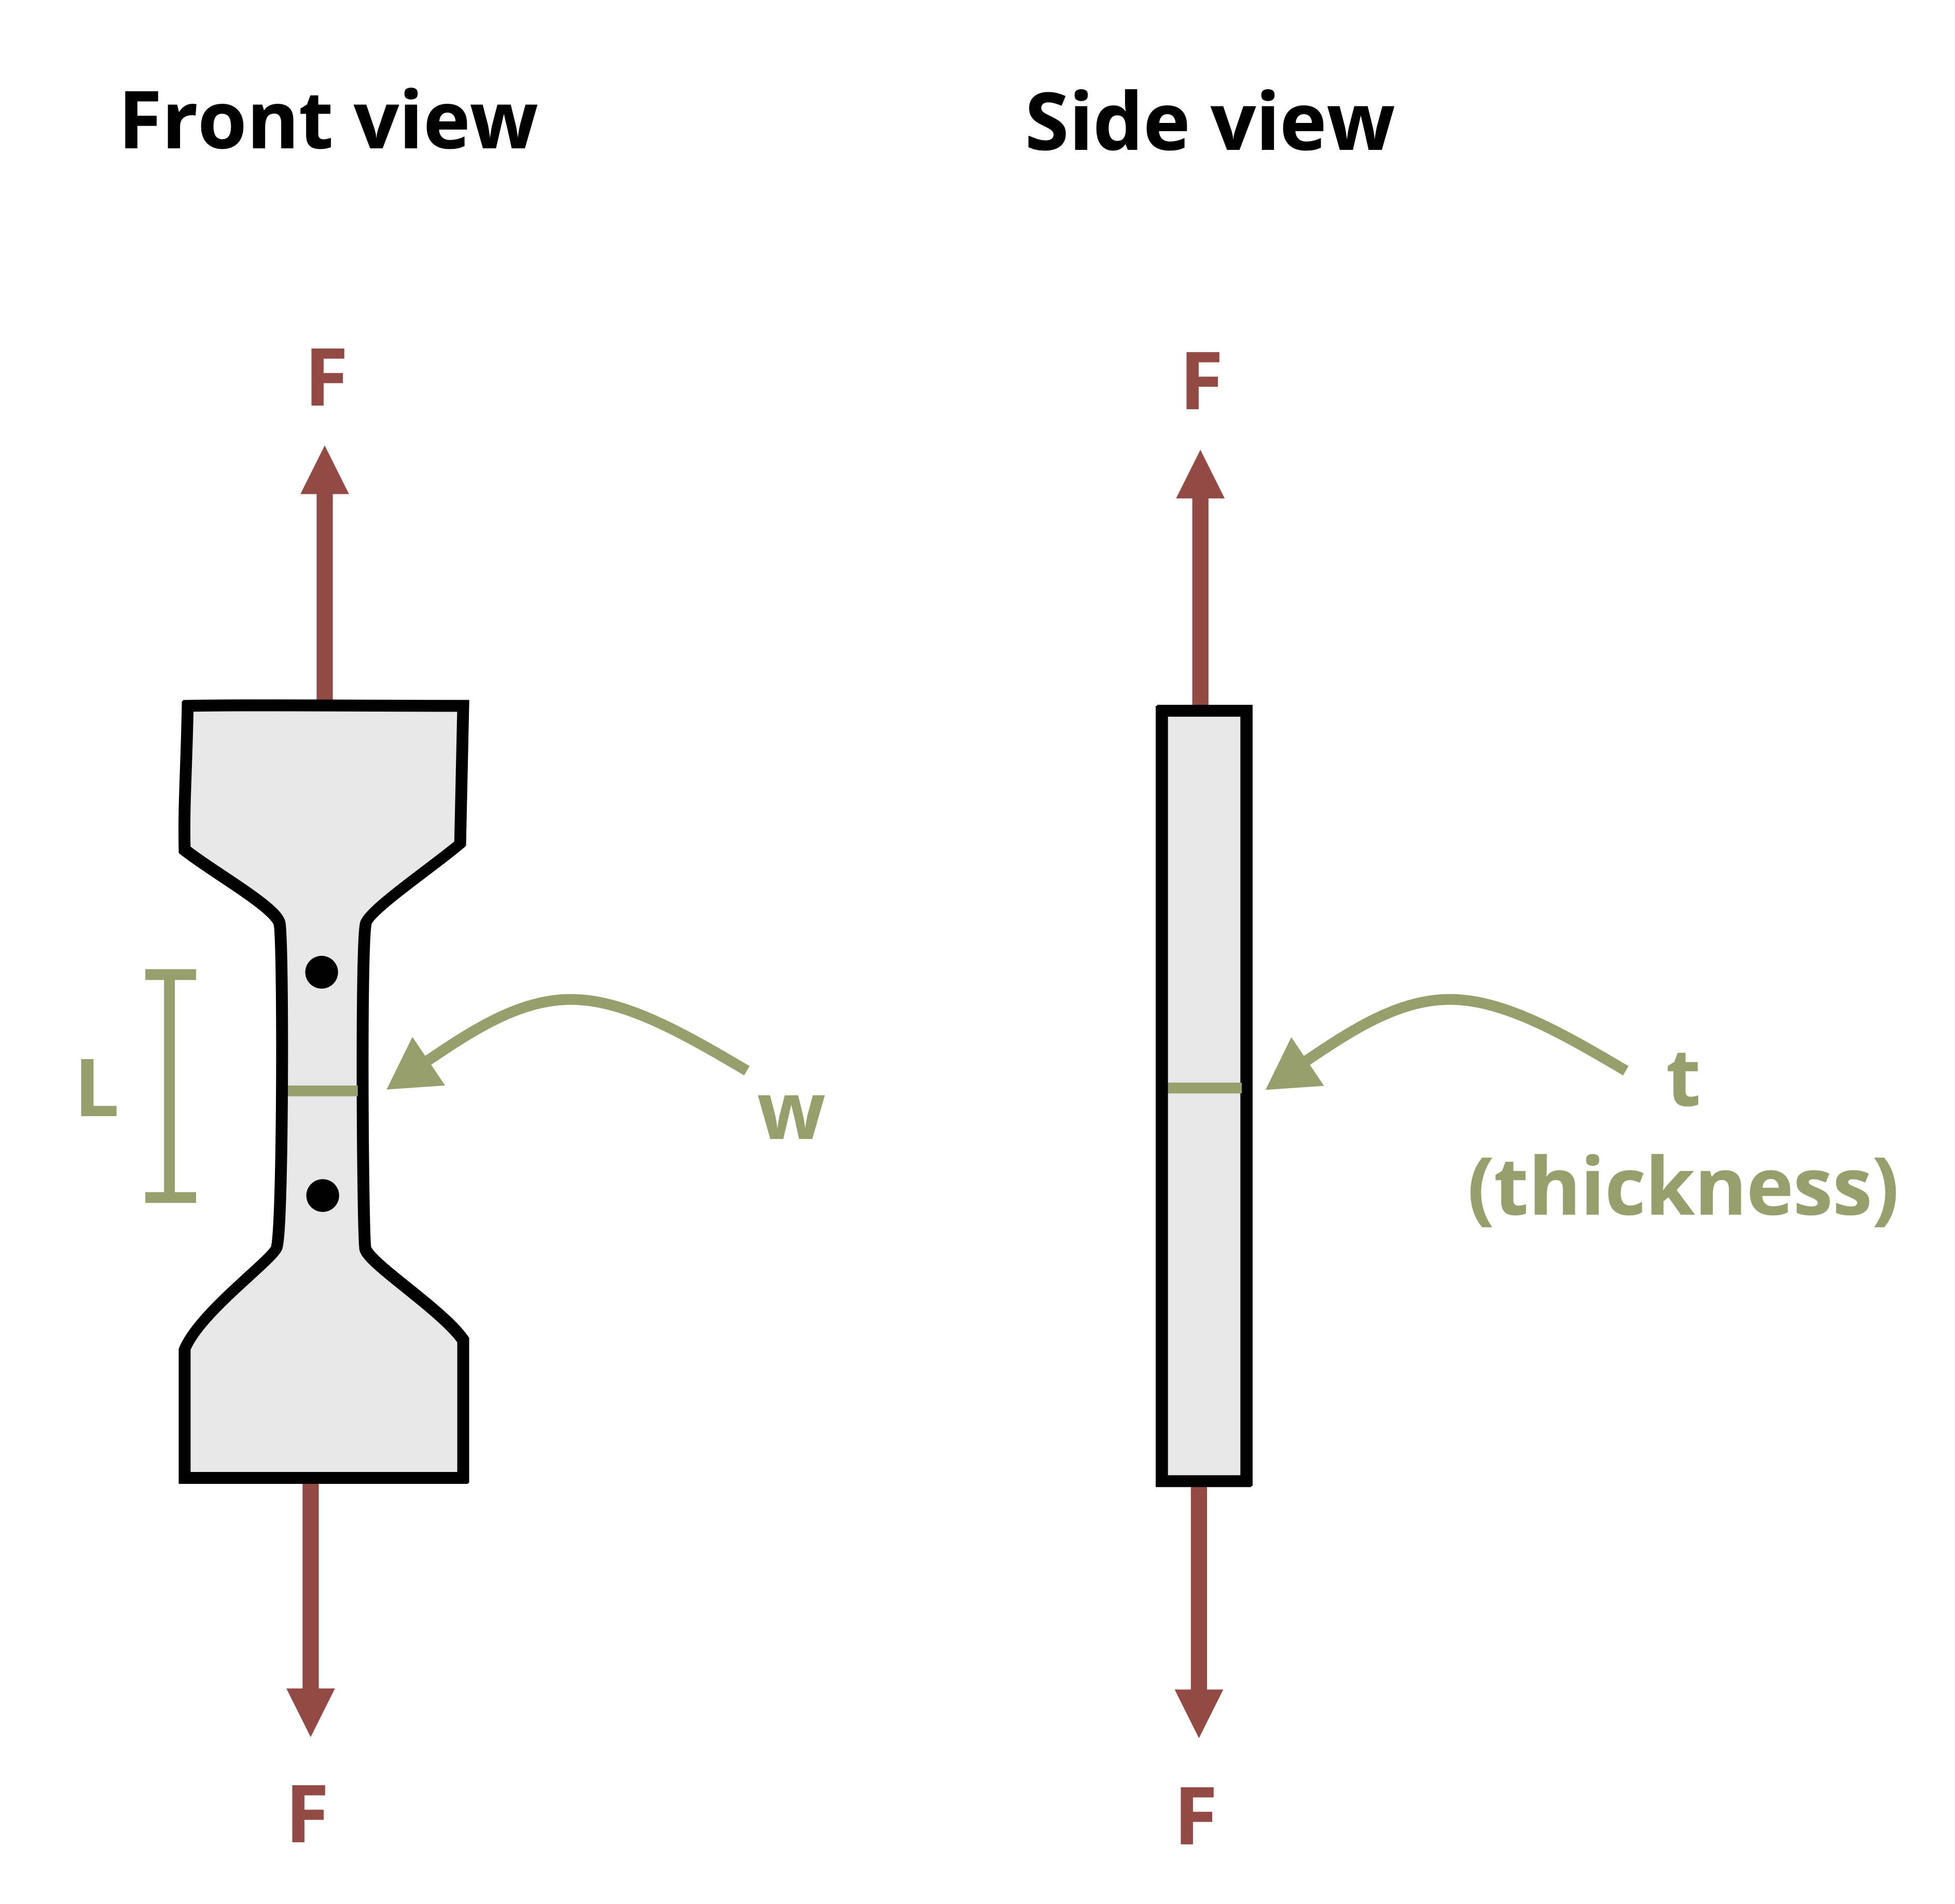
\includegraphics[width=3.125in,height=\textheight,keepaspectratio]{images/194.png}
{[}Problem adapted from © Kurt Gramoll CC BY NC-SA 4.0{]}

\begin{Shaded}
\begin{Highlighting}[]
\NormalTok{\#| standalone: true}
\NormalTok{\#| viewerHeight: 600}
\NormalTok{\#| components: [viewer]}

\NormalTok{from shiny import App, render, ui, reactive}
\NormalTok{import random}
\NormalTok{import asyncio}
\NormalTok{import io}
\NormalTok{import math}
\NormalTok{import string}
\NormalTok{from datetime import datetime}
\NormalTok{from pathlib import Path}

\NormalTok{def generate\_random\_letters(length):}
\NormalTok{    \# Generate a random string of letters of specified length}
\NormalTok{    return \textquotesingle{}\textquotesingle{}.join(random.choice(string.ascii\_lowercase) for \_ in range(length)) }

\NormalTok{problem\_ID="194"}
\NormalTok{F=reactive.Value("\_\_")}
\NormalTok{L=reactive.Value("\_\_")}
\NormalTok{w=reactive.Value("\_\_")}
\NormalTok{t=reactive.Value("\_\_")}
\NormalTok{dL=reactive.Value("\_\_")}


\NormalTok{attempts=["Timestamp,Attempt,Answer,Feedback\textbackslash{}n"]}

\NormalTok{app\_ui = ui.page\_fluid(}
\NormalTok{    ui.markdown("**Please enter your ID number from your instructor and click to generate your problem**"),}
\NormalTok{    ui.input\_text("ID","", placeholder="Enter ID Number Here"),}
\NormalTok{    ui.input\_action\_button("generate\_problem", "Generate Problem", class\_="btn{-}primary"),}
\NormalTok{    ui.markdown("**Problem Statement**"),}
\NormalTok{    ui.output\_ui("ui\_problem\_statement"),}
\NormalTok{    ui.input\_text("answer","Your Answer in units of ksi", placeholder="Please enter your answer"),}
\NormalTok{    ui.input\_action\_button("submit", "Submit Answer", class\_="btn{-}primary"),}
\NormalTok{    ui.download\_button("download", "Download File to Submit", class\_="btn{-}success"),}
\NormalTok{)}


\NormalTok{def server(input, output, session):}
\NormalTok{    \# Initialize a counter for attempts}
\NormalTok{    attempt\_counter = reactive.Value(0)}

\NormalTok{    @output}
\NormalTok{    @render.ui}
\NormalTok{    def ui\_problem\_statement():}
\NormalTok{        return[ui.markdown(f"A polymer test specimen is subjected to an axial load of F = \{F()\} kips. The central portion of the specimen has an initial length L = \{L()\} in., w = \{w()\} in., and t = \{t()\} in. If the length increases by dL = \{dL()\} in., determine the elastic modulus of the material. ")]}
    
\NormalTok{    @reactive.Effect}
\NormalTok{    @reactive.event(input.generate\_problem)}
\NormalTok{    def randomize\_vars():}
\NormalTok{        random.seed(input.ID())}
\NormalTok{        F.set(random.randrange(100, 500, 1)/10)}
\NormalTok{        L.set(random.randrange(50, 150, 1)/10)}
\NormalTok{        w.set(round(L()*0.375, 2))}
\NormalTok{        t.set(random.randrange(10, 50, 1)/100)}
\NormalTok{        dL.set(random.randrange(3, 9, 1)/100)}
        
\NormalTok{    @reactive.Effect}
\NormalTok{    @reactive.event(input.submit)}
\NormalTok{    def \_():}
\NormalTok{        attempt\_counter.set(attempt\_counter() + 1)  \# Increment the attempt counter on each submission.}
\NormalTok{        instr= (F()*L())/(dL()*(w()*t()))}
\NormalTok{        if math.isclose(float(input.answer()), instr, rel\_tol=0.01):}
\NormalTok{            check = "*Correct*"}
\NormalTok{            correct\_indicator = "JL"}
\NormalTok{        else:}
\NormalTok{            check = "*Not Correct.*"}
\NormalTok{            correct\_indicator = "JG"}

\NormalTok{        \# Generate random parts for the encoded attempt.}
\NormalTok{        random\_start = generate\_random\_letters(4)}
\NormalTok{        random\_middle = generate\_random\_letters(4)}
\NormalTok{        random\_end = generate\_random\_letters(4)}
\NormalTok{        encoded\_attempt = f"\{random\_start\}\{problem\_ID\}{-}\{random\_middle\}\{attempt\_counter()\}\{correct\_indicator\}{-}\{random\_end\}\{input.ID()\}"}

\NormalTok{        \# Store the most recent encoded attempt in a reactive value so it persists across submissions}
\NormalTok{        session.encoded\_attempt = reactive.Value(encoded\_attempt)}

\NormalTok{        \# Append the attempt data to the attempts list without the encoded attempt}
\NormalTok{        attempts.append(f"\{datetime.now()\}, \{attempt\_counter()\}, \{input.answer()\}, \{check\}\textbackslash{}n")}

\NormalTok{        \# Show feedback to the user.}
\NormalTok{        feedback = ui.markdown(f"Your answer of \{input.answer()\} is \{check\}.")}
\NormalTok{        m = ui.modal(}
\NormalTok{            feedback,}
\NormalTok{            title="Feedback",}
\NormalTok{            easy\_close=True}
\NormalTok{        )}
\NormalTok{        ui.modal\_show(m)}

\NormalTok{    @session.download(filename=lambda: f"Problem\_Log{-}\{problem\_ID\}{-}\{input.ID()\}.csv")}
\NormalTok{    async def download():}
\NormalTok{        \# Start the CSV with the encoded attempt (without label)}
\NormalTok{        final\_encoded = session.encoded\_attempt() if session.encoded\_attempt is not None else "No attempts"}
\NormalTok{        yield f"\{final\_encoded\}\textbackslash{}n\textbackslash{}n"}
        
\NormalTok{        \# Write the header for the remaining CSV data once}
\NormalTok{        yield "Timestamp,Attempt,Answer,Feedback\textbackslash{}n"}
        
\NormalTok{        \# Write the attempts data, ensure that the header from the attempts list is not written again}
\NormalTok{        for attempt in attempts[1:]:  \# Skip the first element which is the header}
\NormalTok{            await asyncio.sleep(0.25)  \# This delay may not be necessary; adjust as needed}
\NormalTok{            yield attempt}


\NormalTok{\# App installation}
\NormalTok{app = App(app\_ui, server)}
\end{Highlighting}
\end{Shaded}

\chapter*{Problem 4.10 - Poisson's
Ratio}\label{problem-4.10---poissons-ratio}
\addcontentsline{toc}{chapter}{Problem 4.10 - Poisson's Ratio}

\markboth{Problem 4.10 - Poisson's Ratio}{Problem 4.10 - Poisson's
Ratio}

\begin{figure}[H]

{\centering \pandocbounded{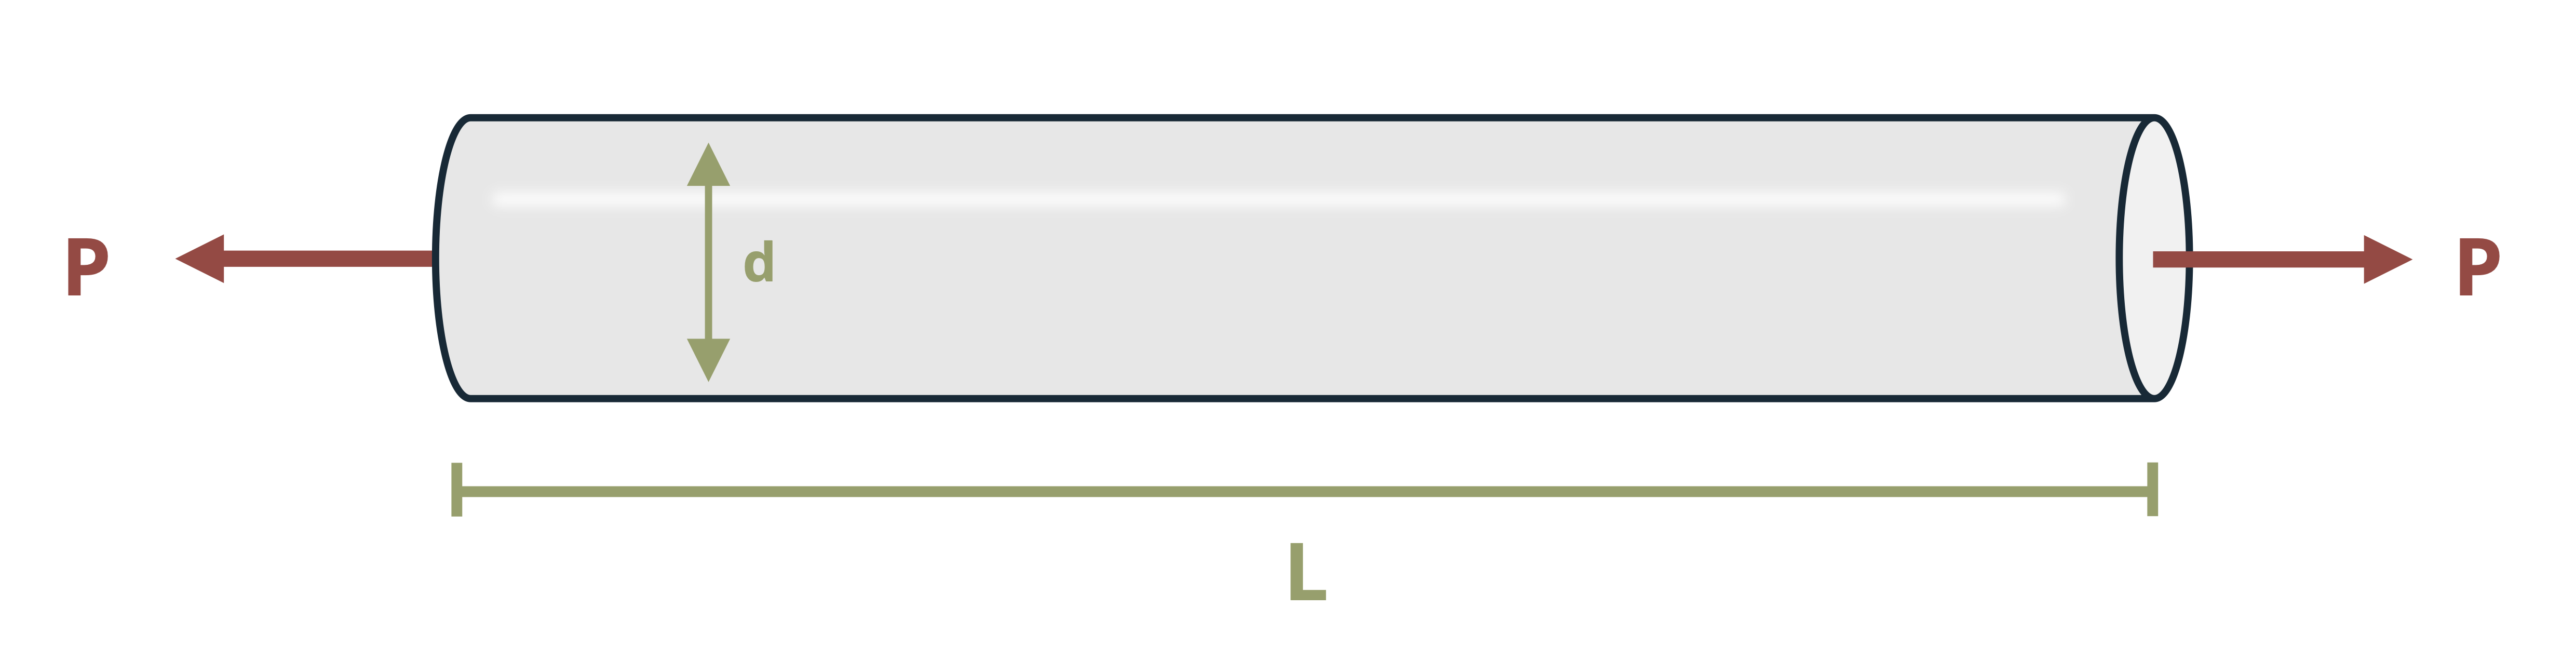
\includegraphics[keepaspectratio]{images/206.png}}

}

\caption{Figure 1: A circular road is placed in tension with an axial
load.}

\end{figure}%

{[}Problem adapted from © Kurt Gramoll CC BY NC-SA 4.0{]}

\begin{Shaded}
\begin{Highlighting}[]
\NormalTok{\#| standalone: true}
\NormalTok{\#| viewerHeight: 600}
\NormalTok{\#| components: [viewer]}

\NormalTok{from shiny import App, render, ui, reactive}
\NormalTok{import random}
\NormalTok{import asyncio}
\NormalTok{import io}
\NormalTok{import math}
\NormalTok{import string}
\NormalTok{from datetime import datetime}
\NormalTok{from pathlib import Path}

\NormalTok{def generate\_random\_letters(length):}
\NormalTok{    \# Generate a random string of letters of specified length}
\NormalTok{    return \textquotesingle{}\textquotesingle{}.join(random.choice(string.ascii\_lowercase) for \_ in range(length)) }

\NormalTok{problem\_ID="206"}
\NormalTok{P=reactive.Value("\_\_")}
\NormalTok{E=reactive.Value("\_\_")}
\NormalTok{L=reactive.Value("\_\_")}
\NormalTok{d=reactive.Value("\_\_")}

\NormalTok{attempts=["Timestamp,Attempt,Answer,Feedback\textbackslash{}n"]}

\NormalTok{app\_ui = ui.page\_fluid(}
\NormalTok{    ui.markdown("**Please enter your ID number from your instructor and click to generate your problem**"),}
\NormalTok{    ui.input\_text("ID","", placeholder="Enter ID Number Here"),}
\NormalTok{    ui.input\_action\_button("generate\_problem", "Generate Problem", class\_="btn{-}primary"),}
\NormalTok{    ui.markdown("**Problem Statement**"),}
\NormalTok{    ui.output\_ui("ui\_problem\_statement"),}
\NormalTok{    ui.input\_text("answer","Your Answer", placeholder="Please enter your answer"),}
\NormalTok{    ui.input\_action\_button("submit", "Submit Answer", class\_="btn{-}primary"),}
\NormalTok{    ui.download\_button("download", "Download File to Submit", class\_="btn{-}success"),}
\NormalTok{)}

\NormalTok{def server(input, output, session):}
\NormalTok{    \# Initialize a counter for attempts}
\NormalTok{    attempt\_counter = reactive.Value(0)}

\NormalTok{    @output}
\NormalTok{    @render.ui}
\NormalTok{    def ui\_problem\_statement():}
\NormalTok{        return[ui.markdown(f"A circular rod of an unknown metallic alloy is placed in tension with a P = \{P()\} kip axial load. The length of the rod is L = \{L()\} in. and the diameter is d = \{d()\} in. After applying the load, the rod length increases by 0.0035 in and the diameter decreases by 0.00014 in. What is the Poisson\textquotesingle{}s ratio of the alloy?")]}
    
\NormalTok{    @reactive.Effect}
\NormalTok{    @reactive.event(input.generate\_problem)}
\NormalTok{    def randomize\_vars():}
\NormalTok{        random.seed(input.ID())}
\NormalTok{        P.set(random.randrange(20, 200, 1)/10)}
\NormalTok{        L.set(random.randrange(10, 20, 1))}
\NormalTok{        E.set(random.randrange(20, 40, 1)/100)}
\NormalTok{        d.set(round((.00014*L())/(.0035*E()), 1))}
        
\NormalTok{    @reactive.Effect}
\NormalTok{    @reactive.event(input.submit)}
\NormalTok{    def \_():}
\NormalTok{        attempt\_counter.set(attempt\_counter() + 1)  \# Increment the attempt counter on each submission.}
       
\NormalTok{        instr= {-}({-}.00014/d())/(.0035/L())}
\NormalTok{        if math.isclose(float(input.answer()), instr, rel\_tol=0.01):}
\NormalTok{            check = "*Correct*"}
\NormalTok{            correct\_indicator = "JL"}
\NormalTok{        else:}
\NormalTok{            check = "*Not Correct.*"}
\NormalTok{            correct\_indicator = "JG"}

\NormalTok{        \# Generate random parts for the encoded attempt.}
\NormalTok{        random\_start = generate\_random\_letters(4)}
\NormalTok{        random\_middle = generate\_random\_letters(4)}
\NormalTok{        random\_end = generate\_random\_letters(4)}
\NormalTok{        encoded\_attempt = f"\{random\_start\}\{problem\_ID\}{-}\{random\_middle\}\{attempt\_counter()\}\{correct\_indicator\}{-}\{random\_end\}\{input.ID()\}"}

\NormalTok{        \# Store the most recent encoded attempt in a reactive value so it persists across submissions}
\NormalTok{        session.encoded\_attempt = reactive.Value(encoded\_attempt)}

\NormalTok{        \# Append the attempt data to the attempts list without the encoded attempt}
\NormalTok{        attempts.append(f"\{datetime.now()\}, \{attempt\_counter()\}, \{input.answer()\}, \{check\}\textbackslash{}n")}

\NormalTok{        \# Show feedback to the user.}
\NormalTok{        feedback = ui.markdown(f"Your answer of \{input.answer()\} is \{check\}.")}
\NormalTok{        m = ui.modal(}
\NormalTok{            feedback,}
\NormalTok{            title="Feedback",}
\NormalTok{            easy\_close=True}
\NormalTok{        )}
\NormalTok{        ui.modal\_show(m)}

\NormalTok{    @session.download(filename=lambda: f"Problem\_Log{-}\{problem\_ID\}{-}\{input.ID()\}.csv")}
\NormalTok{    async def download():}
\NormalTok{        \# Start the CSV with the encoded attempt (without label)}
\NormalTok{        final\_encoded = session.encoded\_attempt() if session.encoded\_attempt is not None else "No attempts"}
\NormalTok{        yield f"\{final\_encoded\}\textbackslash{}n\textbackslash{}n"}
        
\NormalTok{        \# Write the header for the remaining CSV data once}
\NormalTok{        yield "Timestamp,Attempt,Answer,Feedback\textbackslash{}n"}
        
\NormalTok{        \# Write the attempts data, ensure that the header from the attempts list is not written again}
\NormalTok{        for attempt in attempts[1:]:  \# Skip the first element which is the header}
\NormalTok{            await asyncio.sleep(0.25)  \# This delay may not be necessary; adjust as needed}
\NormalTok{            yield attempt}

\NormalTok{\# App installation}
\NormalTok{app = App(app\_ui, server)}
\end{Highlighting}
\end{Shaded}

\chapter*{Problem 4.11 - Poisson's
Ratio}\label{problem-4.11---poissons-ratio}
\addcontentsline{toc}{chapter}{Problem 4.11 - Poisson's Ratio}

\markboth{Problem 4.11 - Poisson's Ratio}{Problem 4.11 - Poisson's
Ratio}

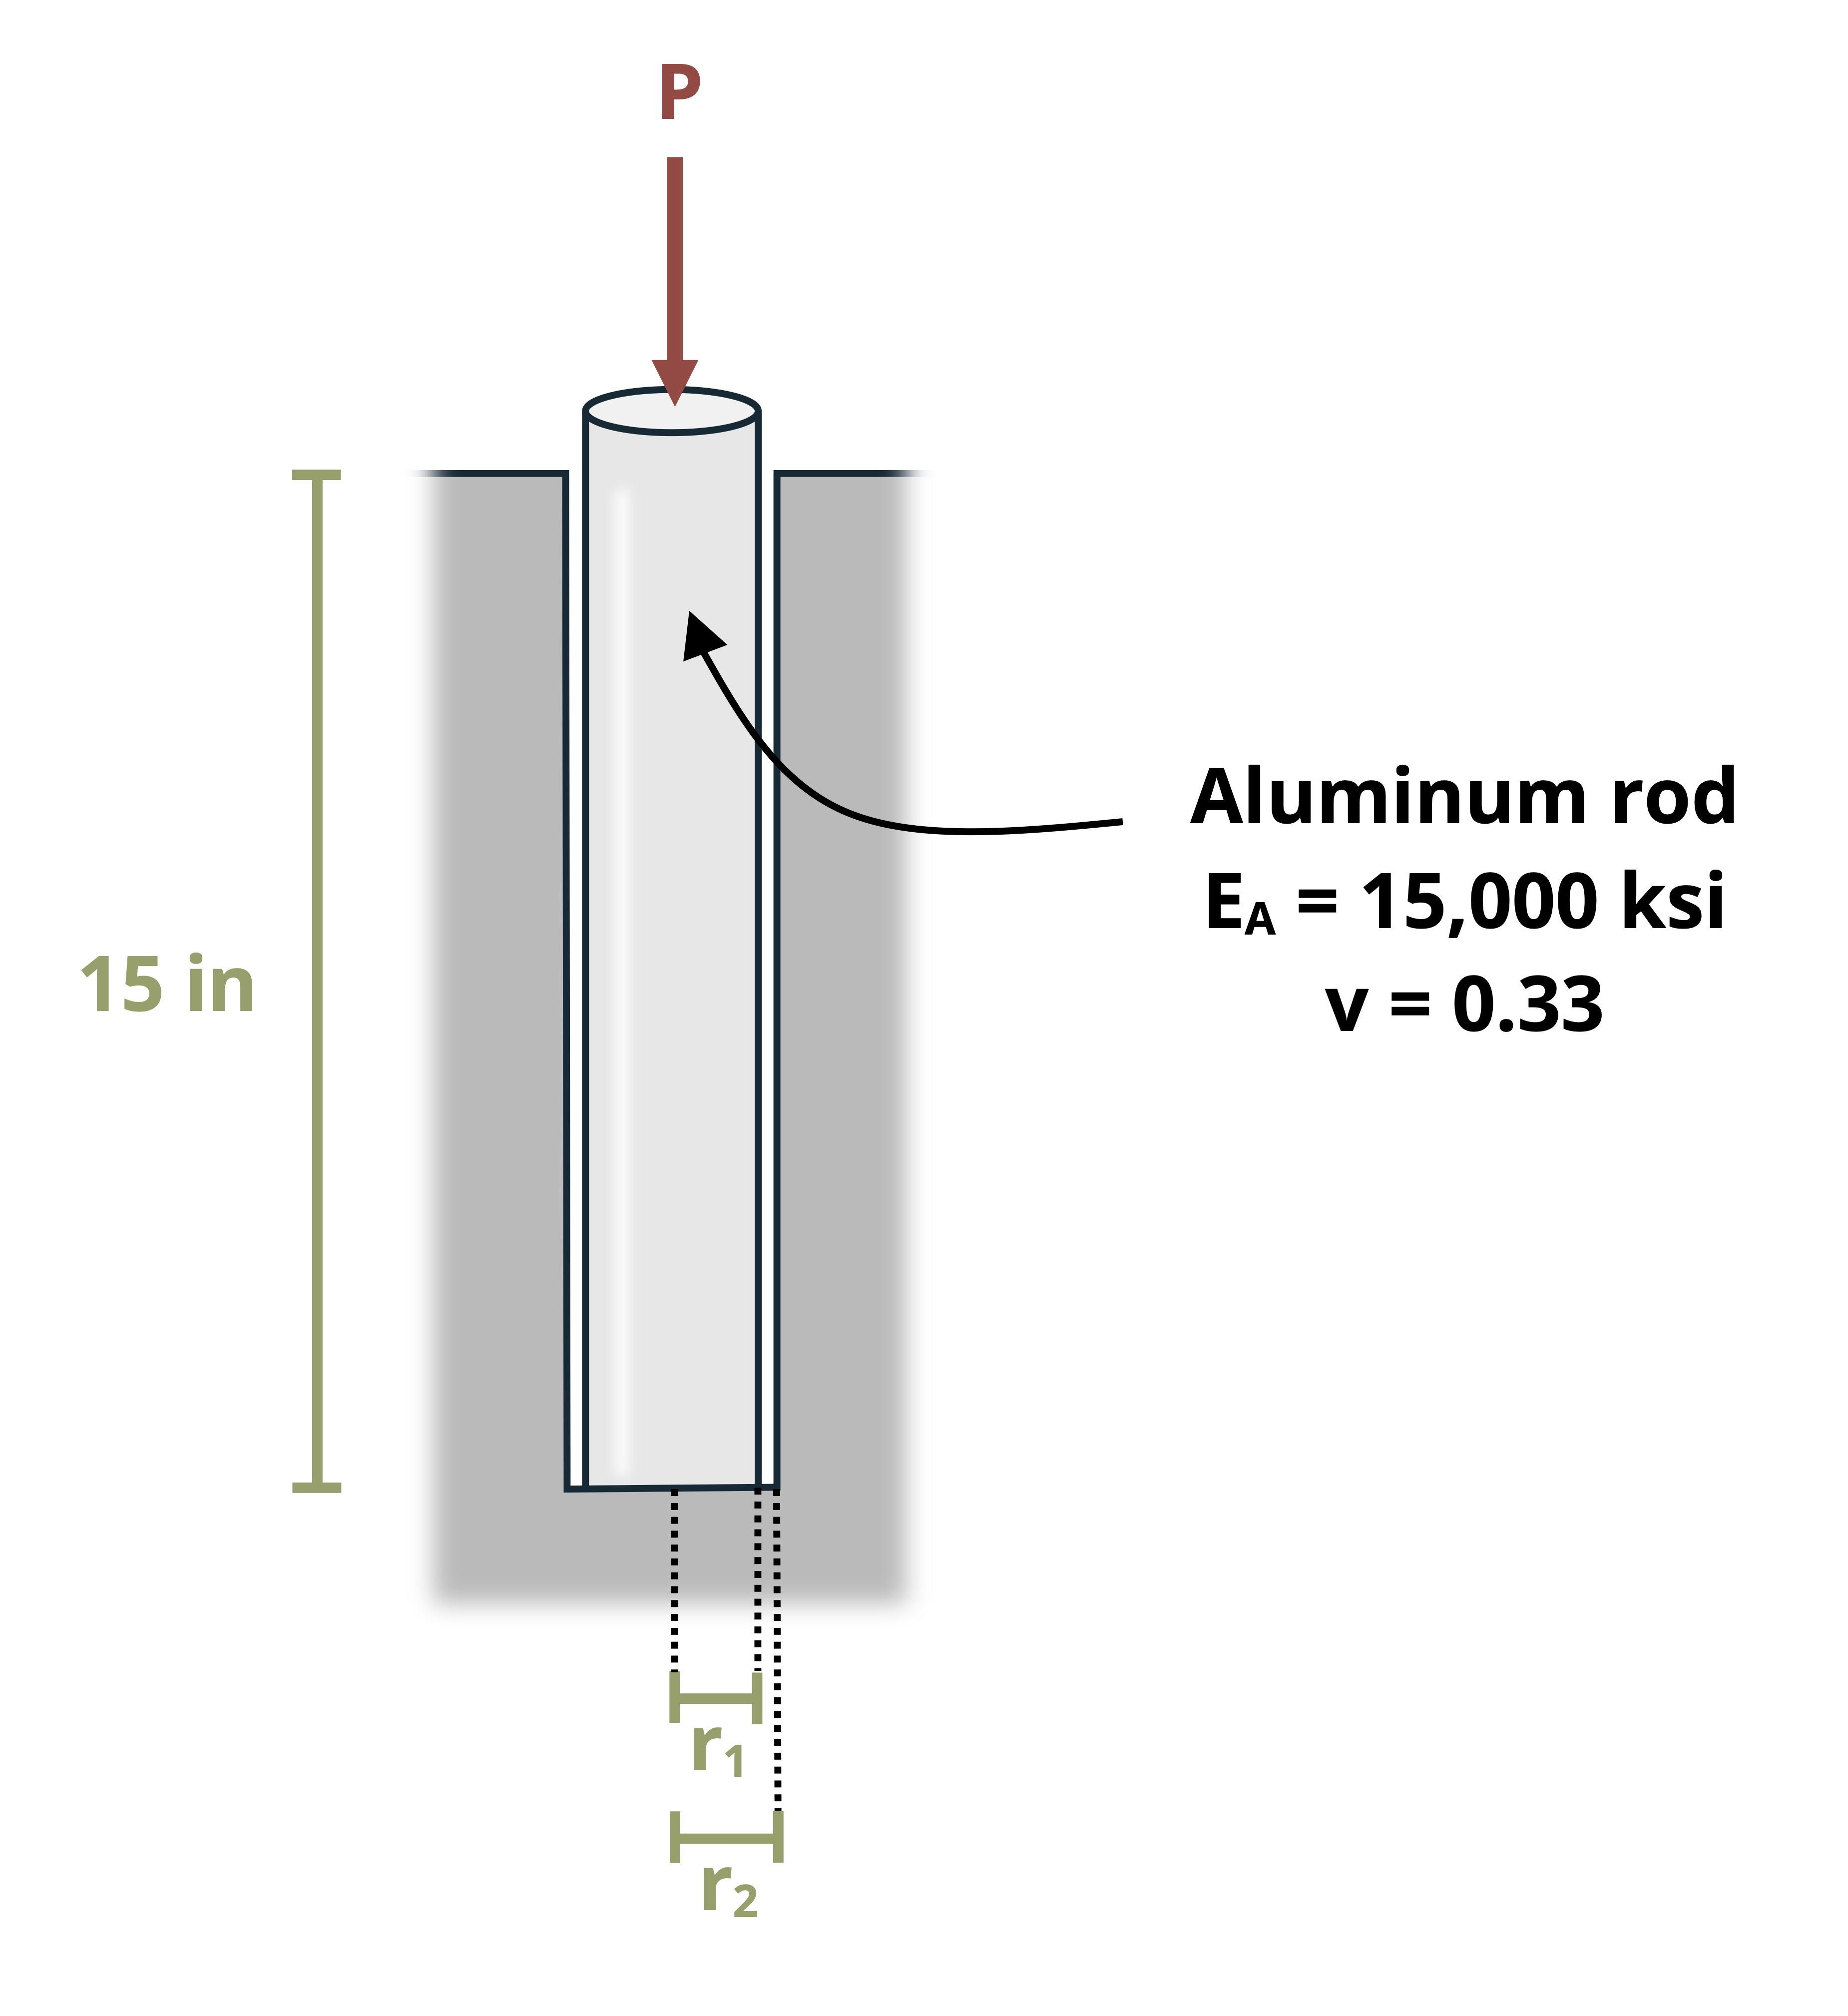
\includegraphics[width=4.16667in,height=\textheight,keepaspectratio]{images/213.png}
{[}Problem adapted from © Kurt Gramoll CC BY NC-SA 4.0{]}

\begin{Shaded}
\begin{Highlighting}[]
\NormalTok{\#| standalone: true}
\NormalTok{\#| viewerHeight: 600}
\NormalTok{\#| components: [viewer]}

\NormalTok{from shiny import App, render, ui, reactive}
\NormalTok{import random}
\NormalTok{import asyncio}
\NormalTok{import io}
\NormalTok{import math}
\NormalTok{import string}
\NormalTok{from datetime import datetime}
\NormalTok{from pathlib import Path}

\NormalTok{def generate\_random\_letters(length):}
\NormalTok{    \# Generate a random string of letters of specified length}
\NormalTok{    return \textquotesingle{}\textquotesingle{}.join(random.choice(string.ascii\_lowercase) for \_ in range(length)) }

\NormalTok{problem\_ID="213"}
\NormalTok{r1=reactive.Value("\_\_")}
\NormalTok{r2=reactive.Value("\_\_")}
\NormalTok{E=15000}
\NormalTok{v=0.33}


\NormalTok{attempts=["Timestamp,Attempt,Answer,Feedback\textbackslash{}n"]}

\NormalTok{app\_ui = ui.page\_fluid(}
\NormalTok{    ui.markdown("**Please enter your ID number from your instructor and click to generate your problem**"),}
\NormalTok{    ui.input\_text("ID","", placeholder="Enter ID Number Here"),}
\NormalTok{    ui.input\_action\_button("generate\_problem", "Generate Problem", class\_="btn{-}primary"),}
\NormalTok{    ui.markdown("**Problem Statement**"),}
\NormalTok{    ui.output\_ui("ui\_problem\_statement"),}
\NormalTok{    ui.input\_text("answer","Your Answer in units of kip", placeholder="Please enter your answer"),}
\NormalTok{    ui.input\_action\_button("submit", "Submit Answer", class\_="btn{-}primary"),}
\NormalTok{    ui.download\_button("download", "Download File to Submit", class\_="btn{-}success"),}
\NormalTok{)}


\NormalTok{def server(input, output, session):}
\NormalTok{    \# Initialize a counter for attempts}
\NormalTok{    attempt\_counter = reactive.Value(0)}

\NormalTok{    @output}
\NormalTok{    @render.ui}
\NormalTok{    def ui\_problem\_statement():}
\NormalTok{        return[ui.markdown(f"An aluminum circular rod of radius r\textless{}sub\textgreater{}1\textless{}/sub\textgreater{} = \{r1()\} in is inserted into space that is slightly wider than the rod, where r\textless{}sub\textgreater{}2\textless{}/sub\textgreater{} = \{r2()\} in. What load P is needed so that the rod expands and fills the space in the radial direction? Assume E = 15,000 ksi and v = 0.33. ")]}
    
\NormalTok{    @reactive.Effect}
\NormalTok{    @reactive.event(input.generate\_problem)}
\NormalTok{    def randomize\_vars():}
\NormalTok{        random.seed(input.ID())}
\NormalTok{        r1.set(random.randrange(10, 50, 1)/10)}
\NormalTok{        r2.set((r1() + random.randrange(1, 10, 1)/1000))}
        
\NormalTok{    @reactive.Effect}
\NormalTok{    @reactive.event(input.submit)}
\NormalTok{    def \_():}
\NormalTok{        attempt\_counter.set(attempt\_counter() + 1)  \# Increment the attempt counter on each submission.}
\NormalTok{        Ex = (r1() {-} r2())/r1()}
\NormalTok{        sigmay = (Ex*E)/({-}v)}
\NormalTok{        instr= sigmay*math.pi*r1()**2}
\NormalTok{        if math.isclose(float(input.answer()), instr, rel\_tol=0.01):}
\NormalTok{            check = "*Correct*"}
\NormalTok{            correct\_indicator = "JL"}
\NormalTok{        else:}
\NormalTok{            check = "*Not Correct.*"}
\NormalTok{            correct\_indicator = "JG"}

\NormalTok{        \# Generate random parts for the encoded attempt.}
\NormalTok{        random\_start = generate\_random\_letters(4)}
\NormalTok{        random\_middle = generate\_random\_letters(4)}
\NormalTok{        random\_end = generate\_random\_letters(4)}
\NormalTok{        encoded\_attempt = f"\{random\_start\}\{problem\_ID\}{-}\{random\_middle\}\{attempt\_counter()\}\{correct\_indicator\}{-}\{random\_end\}\{input.ID()\}"}

\NormalTok{        \# Store the most recent encoded attempt in a reactive value so it persists across submissions}
\NormalTok{        session.encoded\_attempt = reactive.Value(encoded\_attempt)}

\NormalTok{        \# Append the attempt data to the attempts list without the encoded attempt}
\NormalTok{        attempts.append(f"\{datetime.now()\}, \{attempt\_counter()\}, \{input.answer()\}, \{check\}\textbackslash{}n")}

\NormalTok{        \# Show feedback to the user.}
\NormalTok{        feedback = ui.markdown(f"Your answer of \{input.answer()\} is \{check\}.")}
\NormalTok{        m = ui.modal(}
\NormalTok{            feedback,}
\NormalTok{            title="Feedback",}
\NormalTok{            easy\_close=True}
\NormalTok{        )}
\NormalTok{        ui.modal\_show(m)}

\NormalTok{    @session.download(filename=lambda: f"Problem\_Log{-}\{problem\_ID\}{-}\{input.ID()\}.csv")}
\NormalTok{    async def download():}
\NormalTok{        \# Start the CSV with the encoded attempt (without label)}
\NormalTok{        final\_encoded = session.encoded\_attempt() if session.encoded\_attempt is not None else "No attempts"}
\NormalTok{        yield f"\{final\_encoded\}\textbackslash{}n\textbackslash{}n"}
        
\NormalTok{        \# Write the header for the remaining CSV data once}
\NormalTok{        yield "Timestamp,Attempt,Answer,Feedback\textbackslash{}n"}
        
\NormalTok{        \# Write the attempts data, ensure that the header from the attempts list is not written again}
\NormalTok{        for attempt in attempts[1:]:  \# Skip the first element which is the header}
\NormalTok{            await asyncio.sleep(0.25)  \# This delay may not be necessary; adjust as needed}
\NormalTok{            yield attempt}


\NormalTok{\# App installation}
\NormalTok{app = App(app\_ui, server)}
\end{Highlighting}
\end{Shaded}

\chapter*{Problem 4.12 - Poisson's
Ratio}\label{problem-4.12---poissons-ratio}
\addcontentsline{toc}{chapter}{Problem 4.12 - Poisson's Ratio}

\markboth{Problem 4.12 - Poisson's Ratio}{Problem 4.12 - Poisson's
Ratio}

\pandocbounded{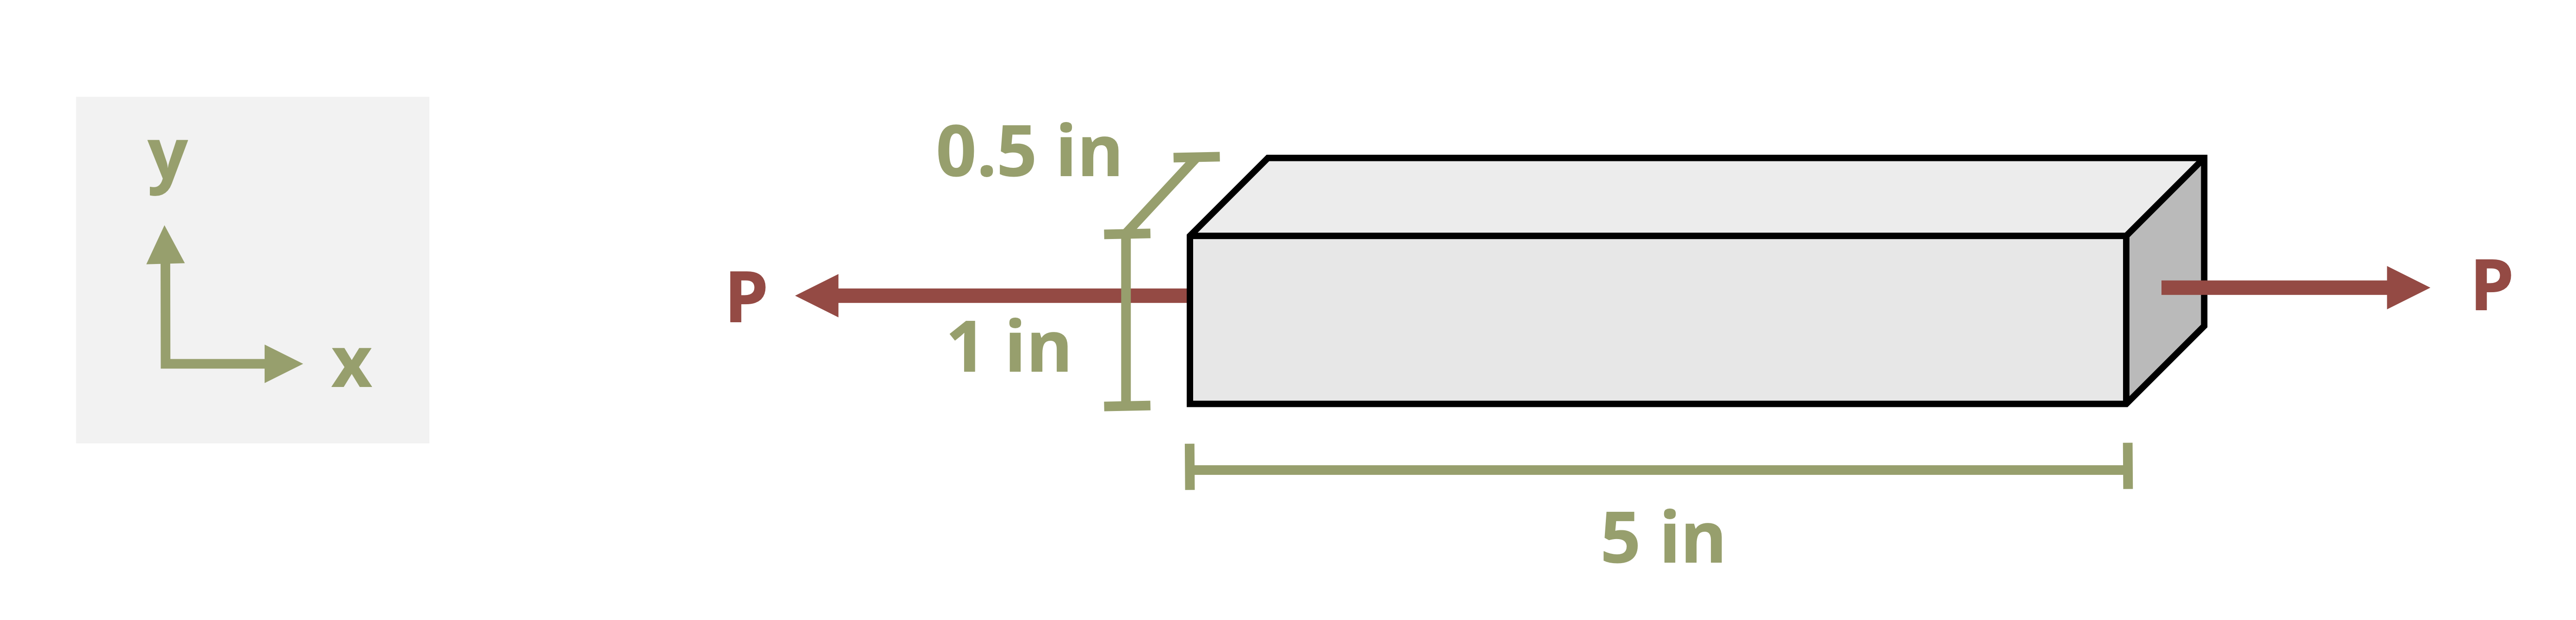
\includegraphics[keepaspectratio]{images/216.png}}
{[}Problem adapted from © Kurt Gramoll CC BY NC-SA 4.0{]}

\begin{Shaded}
\begin{Highlighting}[]
\NormalTok{\#| standalone: true}
\NormalTok{\#| viewerHeight: 600}
\NormalTok{\#| components: [viewer]}

\NormalTok{from shiny import App, render, ui, reactive}
\NormalTok{import random}
\NormalTok{import asyncio}
\NormalTok{import io}
\NormalTok{import math}
\NormalTok{import string}
\NormalTok{from datetime import datetime}
\NormalTok{from pathlib import Path}

\NormalTok{def generate\_random\_letters(length):}
\NormalTok{    \# Generate a random string of letters of specified length}
\NormalTok{    return \textquotesingle{}\textquotesingle{}.join(random.choice(string.ascii\_lowercase) for \_ in range(length)) }

\NormalTok{problem\_ID="216"}
\NormalTok{d1=reactive.Value("\_\_")}
\NormalTok{d2=reactive.Value("\_\_")}


\NormalTok{attempts=["Timestamp,Attempt,Answer,Feedback\textbackslash{}n"]}

\NormalTok{app\_ui = ui.page\_fluid(}
\NormalTok{    ui.markdown("**Please enter your ID number from your instructor and click to generate your problem**"),}
\NormalTok{    ui.input\_text("ID","", placeholder="Enter ID Number Here"),}
\NormalTok{    ui.input\_action\_button("generate\_problem", "Generate Problem", class\_="btn{-}primary"),}
\NormalTok{    ui.markdown("**Problem Statement**"),}
\NormalTok{    ui.output\_ui("ui\_problem\_statement"),}
\NormalTok{    ui.input\_text("answer","Your Answer", placeholder="Please enter your answer"),}
\NormalTok{    ui.input\_action\_button("submit", "Submit Answer", class\_="btn{-}primary"),}
\NormalTok{    ui.download\_button("download", "Download File to Submit", class\_="btn{-}success"),}
\NormalTok{)}


\NormalTok{def server(input, output, session):}
\NormalTok{    \# Initialize a counter for attempts}
\NormalTok{    attempt\_counter = reactive.Value(0)}

\NormalTok{    @output}
\NormalTok{    @render.ui}
\NormalTok{    def ui\_problem\_statement():}
\NormalTok{        return[ui.markdown(f"A rectangular bar is pulled in tension by a load P in the x{-}direction. The bar deflects by δ\textless{}sub\textgreater{}1\textless{}/sub\textgreater{} = \{d1()\} in and δ\textless{}sub\textgreater{}2\textless{}/sub\textgreater{} = {-} \{d2()\} in, in the x{-} and y{-}direction, respectively. The length in the x{-}direction is 5 in, and the length in the y direction is 1 in. What is the Poisson\textquotesingle{}s ratio of the material? The z{-}direction deflection is not known. ")]}
    
\NormalTok{    @reactive.Effect}
\NormalTok{    @reactive.event(input.generate\_problem)}
\NormalTok{    def randomize\_vars():}
\NormalTok{        random.seed(input.ID())}
\NormalTok{        d1.set(random.randrange(20, 50, 1)/1000)}
\NormalTok{        d2.set(random.randrange(10, 20, 1)/10000)}
        
\NormalTok{    @reactive.Effect}
\NormalTok{    @reactive.event(input.submit)}
\NormalTok{    def \_():}
\NormalTok{        attempt\_counter.set(attempt\_counter() + 1)  \# Increment the attempt counter on each submission.}
\NormalTok{        instr= {-}({-}d2()/1)/(d1()/5)}
\NormalTok{        if math.isclose(float(input.answer()), instr, rel\_tol=0.01):}
\NormalTok{            check = "*Correct*"}
\NormalTok{            correct\_indicator = "JL"}
\NormalTok{        else:}
\NormalTok{            check = "*Not Correct.*"}
\NormalTok{            correct\_indicator = "JG"}

\NormalTok{        \# Generate random parts for the encoded attempt.}
\NormalTok{        random\_start = generate\_random\_letters(4)}
\NormalTok{        random\_middle = generate\_random\_letters(4)}
\NormalTok{        random\_end = generate\_random\_letters(4)}
\NormalTok{        encoded\_attempt = f"\{random\_start\}\{problem\_ID\}{-}\{random\_middle\}\{attempt\_counter()\}\{correct\_indicator\}{-}\{random\_end\}\{input.ID()\}"}

\NormalTok{        \# Store the most recent encoded attempt in a reactive value so it persists across submissions}
\NormalTok{        session.encoded\_attempt = reactive.Value(encoded\_attempt)}

\NormalTok{        \# Append the attempt data to the attempts list without the encoded attempt}
\NormalTok{        attempts.append(f"\{datetime.now()\}, \{attempt\_counter()\}, \{input.answer()\}, \{check\}\textbackslash{}n")}

\NormalTok{        \# Show feedback to the user.}
\NormalTok{        feedback = ui.markdown(f"Your answer of \{input.answer()\} is \{check\}.")}
\NormalTok{        m = ui.modal(}
\NormalTok{            feedback,}
\NormalTok{            title="Feedback",}
\NormalTok{            easy\_close=True}
\NormalTok{        )}
\NormalTok{        ui.modal\_show(m)}

\NormalTok{    @session.download(filename=lambda: f"Problem\_Log{-}\{problem\_ID\}{-}\{input.ID()\}.csv")}
\NormalTok{    async def download():}
\NormalTok{        \# Start the CSV with the encoded attempt (without label)}
\NormalTok{        final\_encoded = session.encoded\_attempt() if session.encoded\_attempt is not None else "No attempts"}
\NormalTok{        yield f"\{final\_encoded\}\textbackslash{}n\textbackslash{}n"}
        
\NormalTok{        \# Write the header for the remaining CSV data once}
\NormalTok{        yield "Timestamp,Attempt,Answer,Feedback\textbackslash{}n"}
        
\NormalTok{        \# Write the attempts data, ensure that the header from the attempts list is not written again}
\NormalTok{        for attempt in attempts[1:]:  \# Skip the first element which is the header}
\NormalTok{            await asyncio.sleep(0.25)  \# This delay may not be necessary; adjust as needed}
\NormalTok{            yield attempt}


\NormalTok{\# App installation}
\NormalTok{app = App(app\_ui, server)}
\end{Highlighting}
\end{Shaded}

\chapter*{Problem 4.18 - Thermal
Strain}\label{problem-4.18---thermal-strain}
\addcontentsline{toc}{chapter}{Problem 4.18 - Thermal Strain}

\markboth{Problem 4.18 - Thermal Strain}{Problem 4.18 - Thermal Strain}

{[}Problem adapted from © Chris Galitz CC BY NC-SA 4.0{]}

\begin{Shaded}
\begin{Highlighting}[]
\NormalTok{\#| standalone: true}
\NormalTok{\#| viewerHeight: 600}
\NormalTok{\#| components: [viewer]}

\NormalTok{from shiny import App, render, ui, reactive}
\NormalTok{import random}
\NormalTok{import asyncio}
\NormalTok{import io}
\NormalTok{import math}
\NormalTok{import string}
\NormalTok{from datetime import datetime}
\NormalTok{from pathlib import Path}

\NormalTok{def generate\_random\_letters(length):}
\NormalTok{    \# Generate a random string of letters of specified length}
\NormalTok{    return \textquotesingle{}\textquotesingle{}.join(random.choice(string.ascii\_lowercase) for \_ in range(length))  }

\NormalTok{problem\_ID="658"}
\NormalTok{L=reactive.Value("\_\_")}
\NormalTok{Ti=reactive.Value("\_\_")}
\NormalTok{Tf=reactive.Value("\_\_")}

\NormalTok{attempts=["Timestamp,Attempt,Answer,Feedback\textbackslash{}n"]}

\NormalTok{app\_ui = ui.page\_fluid(}
\NormalTok{    ui.markdown("**Please enter your ID number from your instructor and click to generate your problem**"),}
\NormalTok{    ui.input\_text("ID","", placeholder="Enter ID Number Here"),}
\NormalTok{    ui.input\_action\_button("generate\_problem", "Generate Problem", class\_="btn{-}primary"),}
\NormalTok{    ui.markdown("**Problem Statement**"),}
\NormalTok{    ui.output\_ui("ui\_problem\_statement"),}
\NormalTok{    ui.input\_text("answer","Your Answer in units of m/m", placeholder="Please enter your answer"),}
\NormalTok{    ui.input\_action\_button("submit", "Submit Answer", class\_="btn{-}primary"),}
\NormalTok{    ui.download\_button("download", "Download File to Submit", class\_="btn{-}success"),}
\NormalTok{)}

\NormalTok{def server(input, output, session):}
\NormalTok{    \# Initialize a counter for attempts}
\NormalTok{    attempt\_counter = reactive.Value(0)}

\NormalTok{    @output}
\NormalTok{    @render.ui}
\NormalTok{    def ui\_problem\_statement():}
\NormalTok{        return[ui.markdown(f"A copper pipe (α = 17x10\textless{}sup\textgreater{}{-}6\textless{}/sup\textgreater{} /°C) of length L = \{L()\} m is cooled from \{Ti()\}°C to to \{Tf()\}°C. Determine the longitudinal strain in the cooled pipe.")]}
    
\NormalTok{    @reactive.Effect}
\NormalTok{    @reactive.event(input.generate\_problem)}
\NormalTok{    def randomize\_vars():}
\NormalTok{        random.seed(input.ID())}
\NormalTok{        L.set(random.randrange(50, 100, 1)/10)}
\NormalTok{        Ti.set(random.randrange(30, 50, 1))}
\NormalTok{        Tf.set(Ti(){-}random.randrange(10, 25, 1))}
        
\NormalTok{    @reactive.Effect}
\NormalTok{    @reactive.event(input.submit)}
\NormalTok{    def \_():}
\NormalTok{        attempt\_counter.set(attempt\_counter() + 1)  \# Increment the attempt counter on each submission.}
\NormalTok{        instr= 17*10**{-}6*(Tf(){-}Ti())}
\NormalTok{        if math.isclose(float(input.answer()), instr, rel\_tol=0.01):}
\NormalTok{            check = "*Correct*"}
\NormalTok{            correct\_indicator = "JL"}
\NormalTok{        else:}
\NormalTok{            check = "*Not Correct.*"}
\NormalTok{            correct\_indicator = "JG"}

\NormalTok{        \# Generate random parts for the encoded attempt.}
\NormalTok{        random\_start = generate\_random\_letters(4)}
\NormalTok{        random\_middle = generate\_random\_letters(4)}
\NormalTok{        random\_end = generate\_random\_letters(4)}
\NormalTok{        encoded\_attempt = f"\{random\_start\}\{problem\_ID\}{-}\{random\_middle\}\{attempt\_counter()\}\{correct\_indicator\}{-}\{random\_end\}\{input.ID()\}"}

\NormalTok{        \# Store the most recent encoded attempt in a reactive value so it persists across submissions}
\NormalTok{        session.encoded\_attempt = reactive.Value(encoded\_attempt)}

\NormalTok{        \# Append the attempt data to the attempts list without the encoded attempt}
\NormalTok{        attempts.append(f"\{datetime.now()\}, \{attempt\_counter()\}, \{input.answer()\}, \{check\}\textbackslash{}n")}

\NormalTok{        \# Show feedback to the user.}
\NormalTok{        feedback = ui.markdown(f"Your answer of \{input.answer()\} is \{check\}.")}
\NormalTok{        m = ui.modal(}
\NormalTok{            feedback,}
\NormalTok{            title="Feedback",}
\NormalTok{            easy\_close=True}
\NormalTok{        )}
\NormalTok{        ui.modal\_show(m)}

\NormalTok{    @session.download(filename=lambda: f"Problem\_Log{-}\{problem\_ID\}{-}\{input.ID()\}.csv")}
\NormalTok{    async def download():}
\NormalTok{        \# Start the CSV with the encoded attempt (without label)}
\NormalTok{        final\_encoded = session.encoded\_attempt() if session.encoded\_attempt is not None else "No attempts"}
\NormalTok{        yield f"\{final\_encoded\}\textbackslash{}n\textbackslash{}n"}
        
\NormalTok{        \# Write the header for the remaining CSV data once}
\NormalTok{        yield "Timestamp,Attempt,Answer,Feedback\textbackslash{}n"}
        
\NormalTok{        \# Write the attempts data, ensure that the header from the attempts list is not written again}
\NormalTok{        for attempt in attempts[1:]:  \# Skip the first element which is the header}
\NormalTok{            await asyncio.sleep(0.25)  \# This delay may not be necessary; adjust as needed}
\NormalTok{            yield attempt}

\NormalTok{\# App installation}
\NormalTok{app = App(app\_ui, server)}
\end{Highlighting}
\end{Shaded}

\chapter*{Problem 4.19 - Thermal
Strain}\label{problem-4.19---thermal-strain}
\addcontentsline{toc}{chapter}{Problem 4.19 - Thermal Strain}

\markboth{Problem 4.19 - Thermal Strain}{Problem 4.19 - Thermal Strain}

{[}Problem adapted from © Chris Galitz CC BY NC-SA 4.0{]}

\begin{Shaded}
\begin{Highlighting}[]
\NormalTok{\#| standalone: true}
\NormalTok{\#| viewerHeight: 600}
\NormalTok{\#| components: [viewer]}

\NormalTok{from shiny import App, render, ui, reactive}
\NormalTok{import random}
\NormalTok{import asyncio}
\NormalTok{import io}
\NormalTok{import math}
\NormalTok{import string}
\NormalTok{from datetime import datetime}
\NormalTok{from pathlib import Path}

\NormalTok{def generate\_random\_letters(length):}
\NormalTok{    \# Generate a random string of letters of specified length}
\NormalTok{    return \textquotesingle{}\textquotesingle{}.join(random.choice(string.ascii\_lowercase) for \_ in range(length))  }

\NormalTok{problem\_ID="659"}
\NormalTok{L=reactive.Value("\_\_")}
\NormalTok{Ti=reactive.Value("\_\_")}
\NormalTok{Tf=reactive.Value("\_\_")}

\NormalTok{attempts=["Timestamp,Attempt,Answer,Feedback\textbackslash{}n"]}

\NormalTok{app\_ui = ui.page\_fluid(}
\NormalTok{    ui.markdown("**Please enter your ID number from your instructor and click to generate your problem**"),}
\NormalTok{    ui.input\_text("ID","", placeholder="Enter ID Number Here"),}
\NormalTok{    ui.input\_action\_button("generate\_problem", "Generate Problem", class\_="btn{-}primary"),}
\NormalTok{    ui.markdown("**Problem Statement**"),}
\NormalTok{    ui.output\_ui("ui\_problem\_statement"),}
\NormalTok{    ui.input\_text("answer","Your Answer in units of in.", placeholder="Please enter your answer"),}
\NormalTok{    ui.input\_action\_button("submit", "Submit Answer", class\_="btn{-}primary"),}
\NormalTok{    ui.download\_button("download", "Download File to Submit", class\_="btn{-}success"),}
\NormalTok{)}

\NormalTok{def server(input, output, session):}
\NormalTok{    \# Initialize a counter for attempts}
\NormalTok{    attempt\_counter = reactive.Value(0)}

\NormalTok{    @output}
\NormalTok{    @render.ui}
\NormalTok{    def ui\_problem\_statement():}
\NormalTok{        return[ui.markdown(f"Upon plant startup, a steel steam pipe (α = 6.5 x 10\textless{}sup\textgreater{}{-}6\textless{}/sup\textgreater{} /°F) of length L = \{L()\} ft is raised in temperature from an ambiant temperature of \{Ti()\}°F to \{Tf()\}°F. Determine the change in length of the pipe.")]}
    
\NormalTok{    @reactive.Effect}
\NormalTok{    @reactive.event(input.generate\_problem)}
\NormalTok{    def randomize\_vars():}
\NormalTok{        random.seed(input.ID())}
\NormalTok{        L.set(random.randrange(50, 200, 5))}
\NormalTok{        Ti.set(random.randrange(50, 75, 1))}
\NormalTok{        Tf.set(random.randrange(300, 500, 1))}
        
\NormalTok{    @reactive.Effect}
\NormalTok{    @reactive.event(input.submit)}
\NormalTok{    def \_():}
\NormalTok{        attempt\_counter.set(attempt\_counter() + 1)  \# Increment the attempt counter on each submission.}
\NormalTok{        instr= 6.5*10**{-}6*(Tf(){-}Ti())*L()*12}
\NormalTok{        if math.isclose(float(input.answer()), instr, rel\_tol=0.01):}
\NormalTok{            check = "*Correct*"}
\NormalTok{            correct\_indicator = "JL"}
\NormalTok{        else:}
\NormalTok{            check = "*Not Correct.*"}
\NormalTok{            correct\_indicator = "JG"}

\NormalTok{        \# Generate random parts for the encoded attempt.}
\NormalTok{        random\_start = generate\_random\_letters(4)}
\NormalTok{        random\_middle = generate\_random\_letters(4)}
\NormalTok{        random\_end = generate\_random\_letters(4)}
\NormalTok{        encoded\_attempt = f"\{random\_start\}\{problem\_ID\}{-}\{random\_middle\}\{attempt\_counter()\}\{correct\_indicator\}{-}\{random\_end\}\{input.ID()\}"}

\NormalTok{        \# Store the most recent encoded attempt in a reactive value so it persists across submissions}
\NormalTok{        session.encoded\_attempt = reactive.Value(encoded\_attempt)}

\NormalTok{        \# Append the attempt data to the attempts list without the encoded attempt}
\NormalTok{        attempts.append(f"\{datetime.now()\}, \{attempt\_counter()\}, \{input.answer()\}, \{check\}\textbackslash{}n")}

\NormalTok{        \# Show feedback to the user.}
\NormalTok{        feedback = ui.markdown(f"Your answer of \{input.answer()\} is \{check\}.")}
\NormalTok{        m = ui.modal(}
\NormalTok{            feedback,}
\NormalTok{            title="Feedback",}
\NormalTok{            easy\_close=True}
\NormalTok{        )}
\NormalTok{        ui.modal\_show(m)}

\NormalTok{    @session.download(filename=lambda: f"Problem\_Log{-}\{problem\_ID\}{-}\{input.ID()\}.csv")}
\NormalTok{    async def download():}
\NormalTok{        \# Start the CSV with the encoded attempt (without label)}
\NormalTok{        final\_encoded = session.encoded\_attempt() if session.encoded\_attempt is not None else "No attempts"}
\NormalTok{        yield f"\{final\_encoded\}\textbackslash{}n\textbackslash{}n"}
        
\NormalTok{        \# Write the header for the remaining CSV data once}
\NormalTok{        yield "Timestamp,Attempt,Answer,Feedback\textbackslash{}n"}
        
\NormalTok{        \# Write the attempts data, ensure that the header from the attempts list is not written again}
\NormalTok{        for attempt in attempts[1:]:  \# Skip the first element which is the header}
\NormalTok{            await asyncio.sleep(0.25)  \# This delay may not be necessary; adjust as needed}
\NormalTok{            yield attempt}

\NormalTok{\# App installation}
\NormalTok{app = App(app\_ui, server)}
\end{Highlighting}
\end{Shaded}

\chapter*{Problem 4.23 - Multiaxial Hooke's
Law}\label{problem-4.23---multiaxial-hookes-law}
\addcontentsline{toc}{chapter}{Problem 4.23 - Multiaxial Hooke's Law}

\markboth{Problem 4.23 - Multiaxial Hooke's Law}{Problem 4.23 -
Multiaxial Hooke's Law}

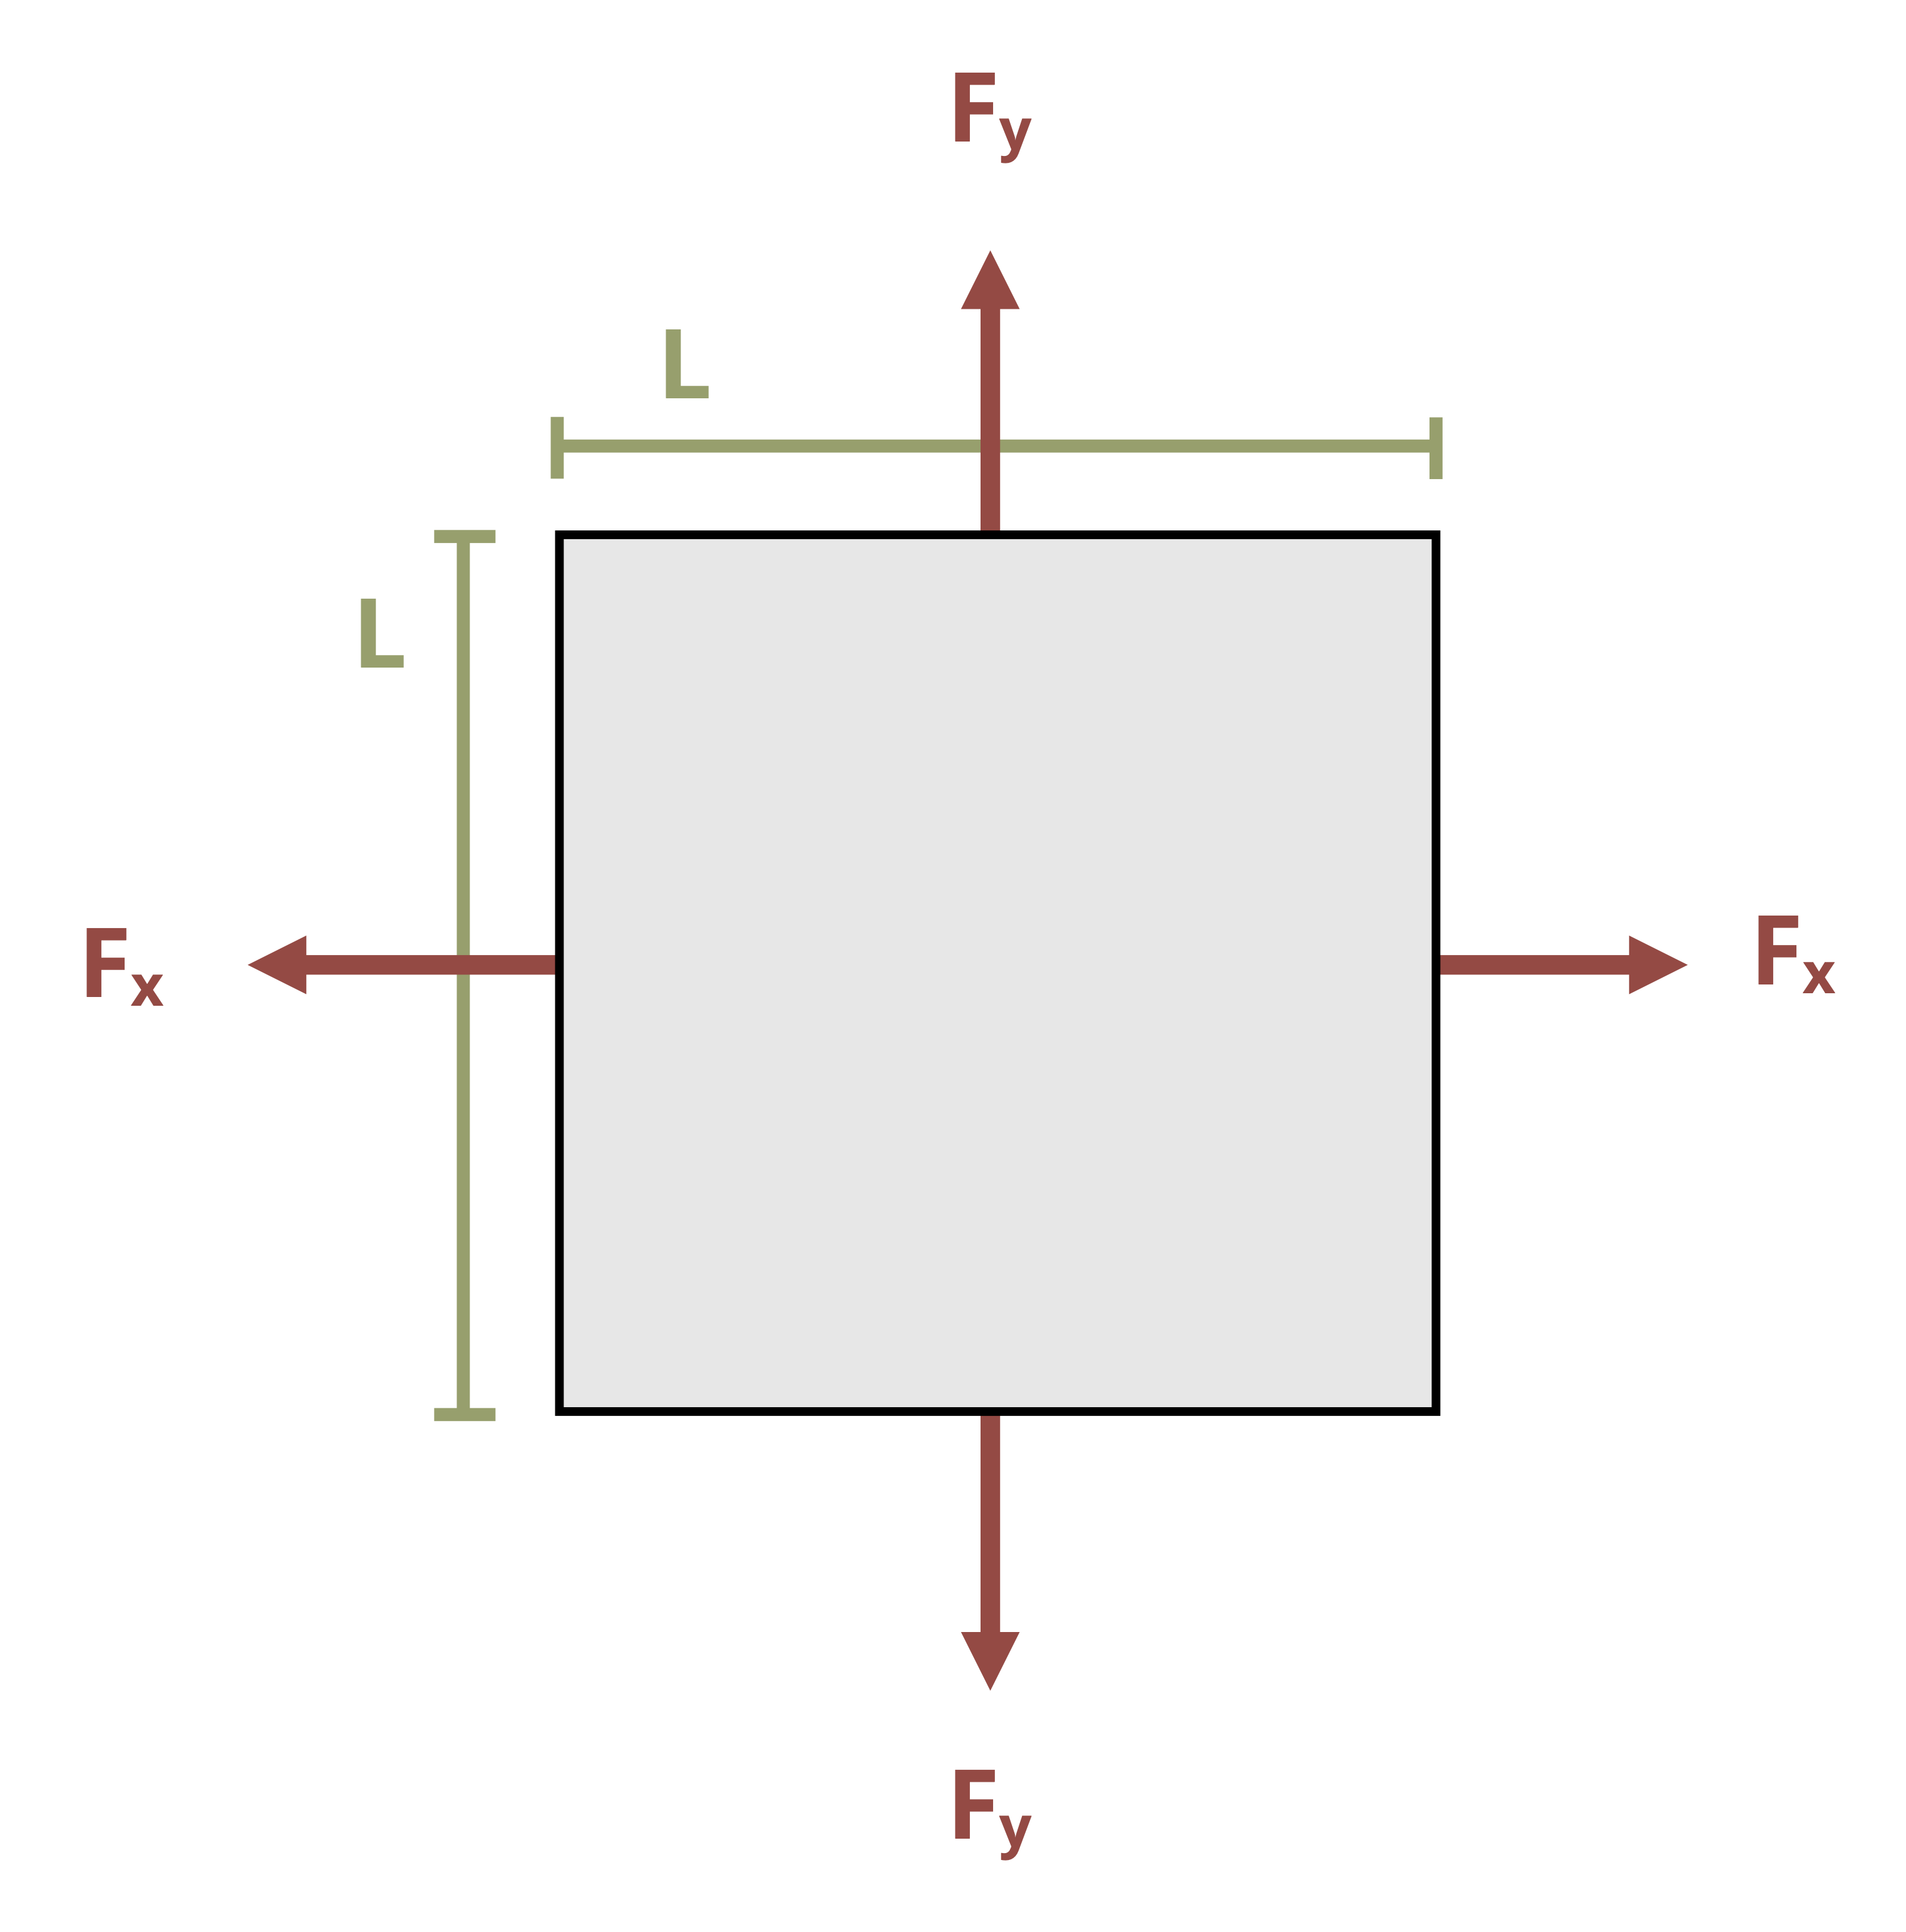
\includegraphics[width=3.125in,height=\textheight,keepaspectratio]{images/204.png}
{[}Problem adapted from © Kurt Gramoll CC BY NC-SA 4.0{]}

\begin{Shaded}
\begin{Highlighting}[]
\NormalTok{\#| standalone: true}
\NormalTok{\#| viewerHeight: 600}
\NormalTok{\#| components: [viewer]}

\NormalTok{from shiny import App, render, ui, reactive}
\NormalTok{import random}
\NormalTok{import asyncio}
\NormalTok{import io}
\NormalTok{import math}
\NormalTok{import string}
\NormalTok{from datetime import datetime}
\NormalTok{from pathlib import Path}

\NormalTok{def generate\_random\_letters(length):}
\NormalTok{    \# Generate a random string of letters of specified length}
\NormalTok{    return \textquotesingle{}\textquotesingle{}.join(random.choice(string.ascii\_lowercase) for \_ in range(length)) }

\NormalTok{problem\_ID="204"}
\NormalTok{L=reactive.Value("\_\_")}
\NormalTok{t=reactive.Value("\_\_")}
\NormalTok{Fx=reactive.Value("\_\_")}
\NormalTok{Fy=reactive.Value("\_\_")}
\NormalTok{E=29000}
\NormalTok{v=0.29}


\NormalTok{attempts=["Timestamp,Attempt,Answer,Feedback\textbackslash{}n"]}

\NormalTok{app\_ui = ui.page\_fluid(}
\NormalTok{    ui.markdown("**Please enter your ID number from your instructor and click to generate your problem**"),}
\NormalTok{    ui.input\_text("ID","", placeholder="Enter ID Number Here"),}
\NormalTok{    ui.input\_action\_button("generate\_problem", "Generate Problem", class\_="btn{-}primary"),}
\NormalTok{    ui.markdown("**Problem Statement**"),}
\NormalTok{    ui.output\_ui("ui\_problem\_statement"),}
\NormalTok{    ui.input\_text("answer","Your Answer in units of inches", placeholder="Please enter your answer"),}
\NormalTok{    ui.input\_action\_button("submit", "Submit Answer", class\_="btn{-}primary"),}
\NormalTok{    ui.download\_button("download", "Download File to Submit", class\_="btn{-}success"),}
\NormalTok{)}


\NormalTok{def server(input, output, session):}
\NormalTok{    \# Initialize a counter for attempts}
\NormalTok{    attempt\_counter = reactive.Value(0)}

\NormalTok{    @output}
\NormalTok{    @render.ui}
\NormalTok{    def ui\_problem\_statement():}
\NormalTok{        return[ui.markdown(f"A square steel plate of side length L = \{L()\} in. and thickness t = \{t()\} in. is uniformly pulled by two forces F\textless{}sub\textgreater{}x\textless{}/sub\textgreater{} = \{Fx()\} kips and F\textless{}sub\textgreater{}y\textless{}/sub\textgreater{} = \{Fy()\} kips as shown. If E = 29,000 ksi and Poisson\textquotesingle{}s ratio v = 0.29, determine the change in thickness of the plate. ")]}
    
\NormalTok{    @reactive.Effect}
\NormalTok{    @reactive.event(input.generate\_problem)}
\NormalTok{    def randomize\_vars():}
\NormalTok{        random.seed(input.ID())}
\NormalTok{        L.set(random.randrange(50, 150, 1)/10)}
\NormalTok{        t.set(random.randrange(2, 10, 1)/10)}
\NormalTok{        Fx.set(random.randrange(100, 500, 1)/10)}
\NormalTok{        Fy.set(random.randrange(100, 500, 1)/10)}
        
\NormalTok{    @reactive.Effect}
\NormalTok{    @reactive.event(input.submit)}
\NormalTok{    def \_():}
\NormalTok{        attempt\_counter.set(attempt\_counter() + 1)  \# Increment the attempt counter on each submission.}
\NormalTok{        sigmax = Fx()/(L()*t())}
\NormalTok{        sigmay = Fy()/(L()*t())}
\NormalTok{        instr= t()*({-}v/E)*(sigmax+sigmay)}
\NormalTok{        if math.isclose(float(input.answer()), instr, rel\_tol=0.01):}
\NormalTok{            check = "*Correct*"}
\NormalTok{            correct\_indicator = "JL"}
\NormalTok{        else:}
\NormalTok{            check = "*Not Correct.*"}
\NormalTok{            correct\_indicator = "JG"}

\NormalTok{        \# Generate random parts for the encoded attempt.}
\NormalTok{        random\_start = generate\_random\_letters(4)}
\NormalTok{        random\_middle = generate\_random\_letters(4)}
\NormalTok{        random\_end = generate\_random\_letters(4)}
\NormalTok{        encoded\_attempt = f"\{random\_start\}\{problem\_ID\}{-}\{random\_middle\}\{attempt\_counter()\}\{correct\_indicator\}{-}\{random\_end\}\{input.ID()\}"}

\NormalTok{        \# Store the most recent encoded attempt in a reactive value so it persists across submissions}
\NormalTok{        session.encoded\_attempt = reactive.Value(encoded\_attempt)}

\NormalTok{        \# Append the attempt data to the attempts list without the encoded attempt}
\NormalTok{        attempts.append(f"\{datetime.now()\}, \{attempt\_counter()\}, \{input.answer()\}, \{check\}\textbackslash{}n")}

\NormalTok{        \# Show feedback to the user.}
\NormalTok{        feedback = ui.markdown(f"Your answer of \{input.answer()\} is \{check\}.")}
\NormalTok{        m = ui.modal(}
\NormalTok{            feedback,}
\NormalTok{            title="Feedback",}
\NormalTok{            easy\_close=True}
\NormalTok{        )}
\NormalTok{        ui.modal\_show(m)}

\NormalTok{    @session.download(filename=lambda: f"Problem\_Log{-}\{problem\_ID\}{-}\{input.ID()\}.csv")}
\NormalTok{    async def download():}
\NormalTok{        \# Start the CSV with the encoded attempt (without label)}
\NormalTok{        final\_encoded = session.encoded\_attempt() if session.encoded\_attempt is not None else "No attempts"}
\NormalTok{        yield f"\{final\_encoded\}\textbackslash{}n\textbackslash{}n"}
        
\NormalTok{        \# Write the header for the remaining CSV data once}
\NormalTok{        yield "Timestamp,Attempt,Answer,Feedback\textbackslash{}n"}
        
\NormalTok{        \# Write the attempts data, ensure that the header from the attempts list is not written again}
\NormalTok{        for attempt in attempts[1:]:  \# Skip the first element which is the header}
\NormalTok{            await asyncio.sleep(0.25)  \# This delay may not be necessary; adjust as needed}
\NormalTok{            yield attempt}


\NormalTok{\# App installation}
\NormalTok{app = App(app\_ui, server)}
\end{Highlighting}
\end{Shaded}

\chapter*{Problem 4.24 - Multiaxial Hooke's
Law}\label{problem-4.24---multiaxial-hookes-law}
\addcontentsline{toc}{chapter}{Problem 4.24 - Multiaxial Hooke's Law}

\markboth{Problem 4.24 - Multiaxial Hooke's Law}{Problem 4.24 -
Multiaxial Hooke's Law}

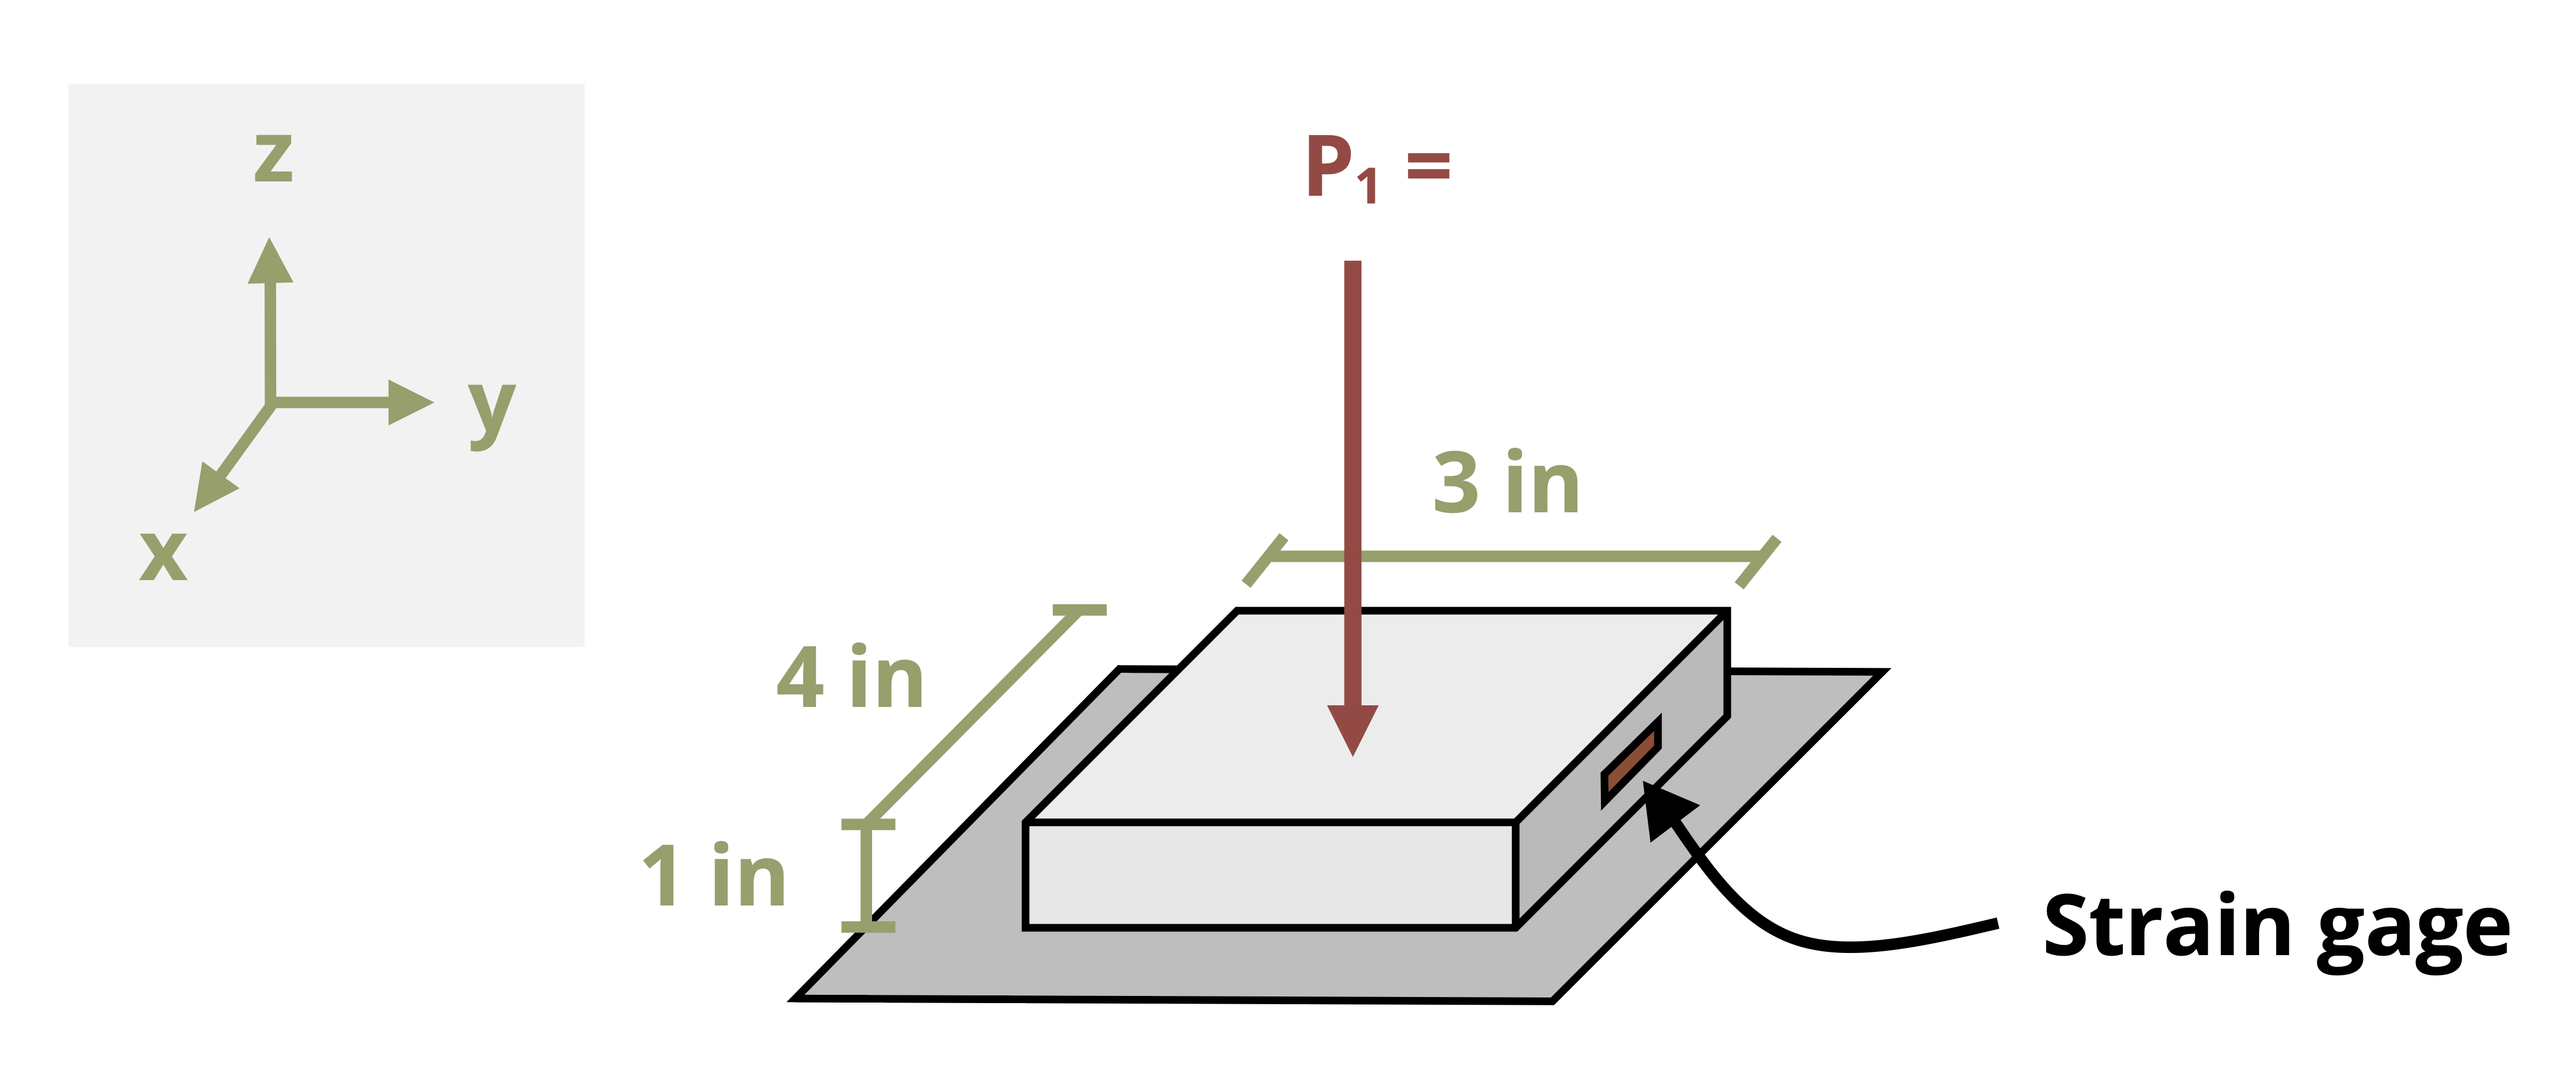
\includegraphics[width=37.44792in,height=\textheight,keepaspectratio]{images/205.png}
{[}Problem adapted from © Kurt Gramoll CC BY NC-SA 4.0{]}

\begin{Shaded}
\begin{Highlighting}[]
\NormalTok{\#| standalone: true}
\NormalTok{\#| viewerHeight: 600}
\NormalTok{\#| components: [viewer]}

\NormalTok{from shiny import App, render, ui, reactive}
\NormalTok{import random}
\NormalTok{import asyncio}
\NormalTok{import io}
\NormalTok{import math}
\NormalTok{import string}
\NormalTok{from datetime import datetime}
\NormalTok{from pathlib import Path}

\NormalTok{def generate\_random\_letters(length):}
\NormalTok{    \# Generate a random string of letters of specified length}
\NormalTok{    return \textquotesingle{}\textquotesingle{}.join(random.choice(string.ascii\_lowercase) for \_ in range(length)) }

\NormalTok{problem\_ID="205"}
\NormalTok{P1=reactive.Value("\_\_")}
\NormalTok{E=reactive.Value("\_\_")}
\NormalTok{v=reactive.Value("\_\_")}
\NormalTok{SG=reactive.Value("\_\_")}

\NormalTok{attempts=["Timestamp,Attempt,Answer,Feedback\textbackslash{}n"]}

\NormalTok{app\_ui = ui.page\_fluid(}
\NormalTok{    ui.markdown("**Please enter your ID number from your instructor and click to generate your problem**"),}
\NormalTok{    ui.input\_text("ID","", placeholder="Enter ID Number Here"),}
\NormalTok{    ui.input\_action\_button("generate\_problem", "Generate Problem", class\_="btn{-}primary"),}
\NormalTok{    ui.markdown("**Problem Statement**"),}
\NormalTok{    ui.output\_ui("ui\_problem\_statement"),}
\NormalTok{    ui.input\_text("answer","Your Answer in percent", placeholder="Please enter your answer"),}
\NormalTok{    ui.input\_action\_button("submit", "Submit Answer", class\_="btn{-}primary"),}
\NormalTok{    ui.download\_button("download", "Download File to Submit", class\_="btn{-}success"),}
\NormalTok{)}

\NormalTok{def server(input, output, session):}
\NormalTok{    \# Initialize a counter for attempts}
\NormalTok{    attempt\_counter = reactive.Value(0)}

\NormalTok{    @output}
\NormalTok{    @render.ui}
\NormalTok{    def ui\_problem\_statement():}
\NormalTok{        return[ui.markdown(f"A strain gauge is placed on a polymer test sample with an elastic modulus E =  \{E()\} x 10\textless{}sup\textgreater{}6\textless{}/sup\textgreater{} psi and a Poisson\textquotesingle{}s ratio of v = \{v()\}. When a P\textless{}sub\textgreater{}1\textless{}/sub\textgreater{} = \{P1()\} kip vertical load is applied to the test sample, the strain gauge reads a strain of ε = \{SG()\} x 10\textless{}sup\textgreater{}{-}6\textless{}/sup\textgreater{} in the x{-}direction. What is the relative error of the strain gauge compared to the theoretical strain of the test sample? Note: relative error is defined to be the difference between the measured value and the theoretical value divided by the theoretical value.")]}
    
\NormalTok{    @reactive.Effect}
\NormalTok{    @reactive.event(input.generate\_problem)}
\NormalTok{    def randomize\_vars():}
\NormalTok{        random.seed(input.ID())}
\NormalTok{        P1.set(random.randrange(20, 200, 1)/10)}
\NormalTok{        E.set(random.randrange(5, 20, 1))}
\NormalTok{        v.set(random.randrange(20, 40, 1)/100)}
\NormalTok{        SG.set(round((v()*P1()*1000)/(12*E()),1){-}(random.randrange(3, 20, 1)/10))}
        
\NormalTok{    @reactive.Effect}
\NormalTok{    @reactive.event(input.submit)}
\NormalTok{    def \_():}
\NormalTok{        attempt\_counter.set(attempt\_counter() + 1)  \# Increment the attempt counter on each submission.}
\NormalTok{        sigmaz = ({-}P1()*1000)/(4*3)}
\NormalTok{        Ex = (({-}v()*(sigmaz))/(E()*10**6))}
\NormalTok{        instr=  ((Ex {-} SG()*10**{-}6)/Ex)*100}
\NormalTok{        if math.isclose(float(input.answer()), instr, rel\_tol=0.01):}
\NormalTok{            check = "*Correct*"}
\NormalTok{            correct\_indicator = "JL"}
\NormalTok{        else:}
\NormalTok{            check = "*Not Correct.*"}
\NormalTok{            correct\_indicator = "JG"}

\NormalTok{        \# Generate random parts for the encoded attempt.}
\NormalTok{        random\_start = generate\_random\_letters(4)}
\NormalTok{        random\_middle = generate\_random\_letters(4)}
\NormalTok{        random\_end = generate\_random\_letters(4)}
\NormalTok{        encoded\_attempt = f"\{random\_start\}\{problem\_ID\}{-}\{random\_middle\}\{attempt\_counter()\}\{correct\_indicator\}{-}\{random\_end\}\{input.ID()\}"}

\NormalTok{        \# Store the most recent encoded attempt in a reactive value so it persists across submissions}
\NormalTok{        session.encoded\_attempt = reactive.Value(encoded\_attempt)}

\NormalTok{        \# Append the attempt data to the attempts list without the encoded attempt}
\NormalTok{        attempts.append(f"\{datetime.now()\}, \{attempt\_counter()\}, \{input.answer()\}, \{check\}\textbackslash{}n")}

\NormalTok{        \# Show feedback to the user.}
\NormalTok{        feedback = ui.markdown(f"Your answer of \{input.answer()\} is \{check\}.")}
\NormalTok{        m = ui.modal(}
\NormalTok{            feedback,}
\NormalTok{            title="Feedback",}
\NormalTok{            easy\_close=True}
\NormalTok{        )}
\NormalTok{        ui.modal\_show(m)}

\NormalTok{    @session.download(filename=lambda: f"Problem\_Log{-}\{problem\_ID\}{-}\{input.ID()\}.csv")}
\NormalTok{    async def download():}
\NormalTok{        \# Start the CSV with the encoded attempt (without label)}
\NormalTok{        final\_encoded = session.encoded\_attempt() if session.encoded\_attempt is not None else "No attempts"}
\NormalTok{        yield f"\{final\_encoded\}\textbackslash{}n\textbackslash{}n"}
        
\NormalTok{        \# Write the header for the remaining CSV data once}
\NormalTok{        yield "Timestamp,Attempt,Answer,Feedback\textbackslash{}n"}
        
\NormalTok{        \# Write the attempts data, ensure that the header from the attempts list is not written again}
\NormalTok{        for attempt in attempts[1:]:  \# Skip the first element which is the header}
\NormalTok{            await asyncio.sleep(0.25)  \# This delay may not be necessary; adjust as needed}
\NormalTok{            yield attempt}

\NormalTok{\# App installation}
\NormalTok{app = App(app\_ui, server)}
\end{Highlighting}
\end{Shaded}

\chapter*{Problem 4.25 - Multiaxial Hooke's
Law}\label{problem-4.25---multiaxial-hookes-law}
\addcontentsline{toc}{chapter}{Problem 4.25 - Multiaxial Hooke's Law}

\markboth{Problem 4.25 - Multiaxial Hooke's Law}{Problem 4.25 -
Multiaxial Hooke's Law}

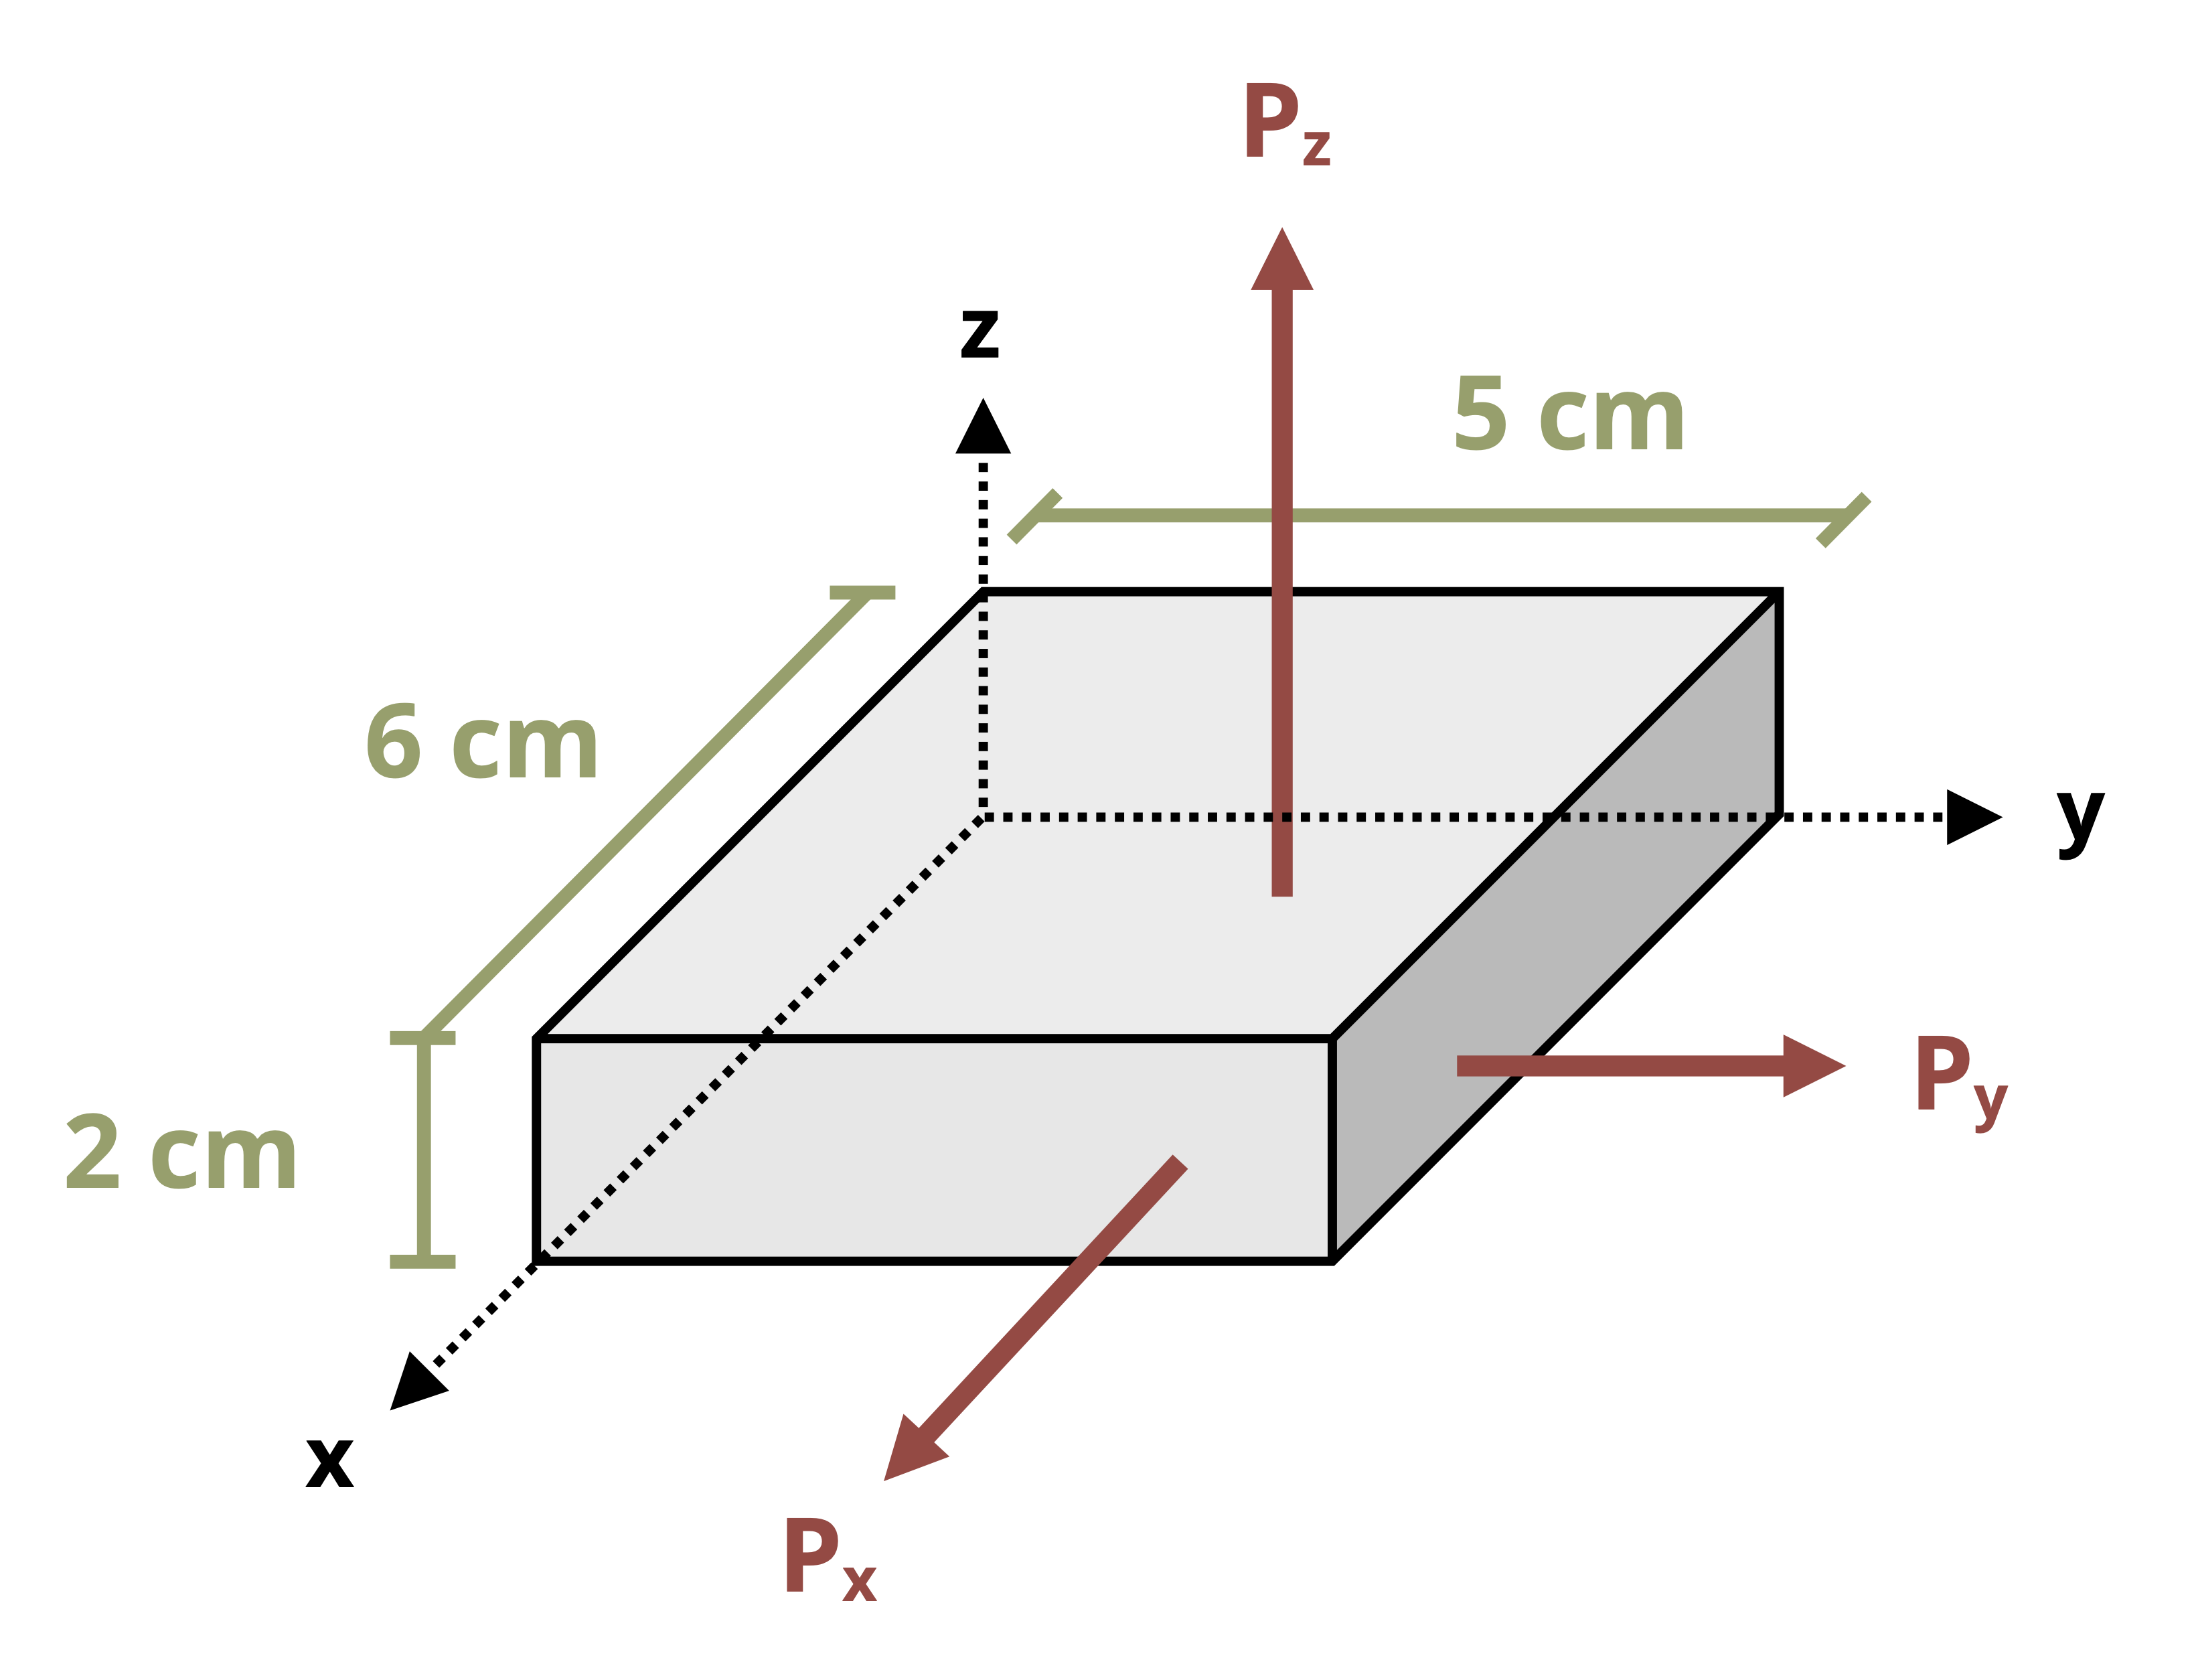
\includegraphics[width=20.40625in,height=\textheight,keepaspectratio]{images/208.png}
{[}Problem adapted from © Kurt Gramoll CC BY NC-SA 4.0{]}

\begin{Shaded}
\begin{Highlighting}[]
\NormalTok{\#| standalone: true}
\NormalTok{\#| viewerHeight: 600}
\NormalTok{\#| components: [viewer]}

\NormalTok{from shiny import App, render, ui, reactive}
\NormalTok{import random}
\NormalTok{import asyncio}
\NormalTok{import io}
\NormalTok{import math}
\NormalTok{import string}
\NormalTok{from datetime import datetime}
\NormalTok{from pathlib import Path}

\NormalTok{def generate\_random\_letters(length):}
\NormalTok{    \# Generate a random string of letters of specified length}
\NormalTok{    return \textquotesingle{}\textquotesingle{}.join(random.choice(string.ascii\_lowercase) for \_ in range(length)) }

\NormalTok{problem\_ID="208"}
\NormalTok{Px=reactive.Value("\_\_")}
\NormalTok{Py=reactive.Value("\_\_")}
\NormalTok{Pz=reactive.Value("\_\_")}
\NormalTok{L=reactive.Value("\_\_")}
\NormalTok{E=reactive.Value("\_\_")}
\NormalTok{v=reactive.Value("\_\_")}


\NormalTok{attempts=["Timestamp,Attempt,Answer,Feedback\textbackslash{}n"]}

\NormalTok{app\_ui = ui.page\_fluid(}
\NormalTok{    ui.markdown("**Please enter your ID number from your instructor and click to generate your problem**"),}
\NormalTok{    ui.input\_text("ID","", placeholder="Enter ID Number Here"),}
\NormalTok{    ui.input\_action\_button("generate\_problem", "Generate Problem", class\_="btn{-}primary"),}
\NormalTok{    ui.markdown("**Problem Statement**"),}
\NormalTok{    ui.output\_ui("ui\_problem\_statement"),}
\NormalTok{    ui.input\_text("answer","Your Answer in percent", placeholder="Please enter your answer"),}
\NormalTok{    ui.input\_action\_button("submit", "Submit Answer", class\_="btn{-}primary"),}
\NormalTok{    ui.download\_button("download", "Download File to Submit", class\_="btn{-}success"),}
\NormalTok{)}


\NormalTok{def server(input, output, session):}
\NormalTok{    \# Initialize a counter for attempts}
\NormalTok{    attempt\_counter = reactive.Value(0)}

\NormalTok{    @output}
\NormalTok{    @render.ui}
\NormalTok{    def ui\_problem\_statement():}
\NormalTok{        return[ui.markdown(f"A block is pulled in all three directions (P\textless{}sub\textgreater{}x\textless{}/sub\textgreater{} = \{Px()\} kN, P\textless{}sub\textgreater{}y\textless{}/sub\textgreater{} = \{Py()\} kN, P\textless{}sub\textgreater{}z\textless{}/sub\textgreater{} = \{Pz()\} kN). What is the percent change in volume after all three loads are applied? Assume E = \{E()\} MPa and v = \{v()\}. ")]}
    
\NormalTok{    @reactive.Effect}
\NormalTok{    @reactive.event(input.generate\_problem)}
\NormalTok{    def randomize\_vars():}
\NormalTok{        random.seed(input.ID())}
\NormalTok{        Px.set(random.randrange(1, 20, 1))}
\NormalTok{        Py.set(random.randrange(1, 20, 1))}
\NormalTok{        Pz.set(random.randrange(1, 20, 1))}
\NormalTok{        E.set(random.randrange(1000, 2000, 100))}
\NormalTok{        v.set(random.randrange(20, 40, 1)/100)}
        
\NormalTok{    @reactive.Effect}
\NormalTok{    @reactive.event(input.submit)}
\NormalTok{    def \_():}
\NormalTok{        attempt\_counter.set(attempt\_counter() + 1)  \# Increment the attempt counter on each submission.}
\NormalTok{        sigmax = (Px()/(5*2))*10}
\NormalTok{        sigmay = (Py()/(6*2))*10}
\NormalTok{        sigmaz = (Pz()/(5*6))*10}
\NormalTok{        Ex = (sigmax {-} v()*(sigmay+sigmaz))/(E())}
\NormalTok{        Ey = (sigmay {-} v()*(sigmaz+sigmax))/(E())}
\NormalTok{        Ez = (sigmaz {-} v()*(sigmax+sigmay))/(E())}
\NormalTok{        Lx = 6 + 6*Ex}
\NormalTok{        Ly = 5 + 5*Ey}
\NormalTok{        Lz = 2 + 2*Ez}
\NormalTok{        instr= (((Lx*Ly*Lz){-}60)/60)*100}
\NormalTok{        if math.isclose(float(input.answer()), instr, rel\_tol=0.01):}
\NormalTok{            check = "*Correct*"}
\NormalTok{            correct\_indicator = "JL"}
\NormalTok{        else:}
\NormalTok{            check = "*Not Correct.*"}
\NormalTok{            correct\_indicator = "JG"}

\NormalTok{        \# Generate random parts for the encoded attempt.}
\NormalTok{        random\_start = generate\_random\_letters(4)}
\NormalTok{        random\_middle = generate\_random\_letters(4)}
\NormalTok{        random\_end = generate\_random\_letters(4)}
\NormalTok{        encoded\_attempt = f"\{random\_start\}\{problem\_ID\}{-}\{random\_middle\}\{attempt\_counter()\}\{correct\_indicator\}{-}\{random\_end\}\{input.ID()\}"}

\NormalTok{        \# Store the most recent encoded attempt in a reactive value so it persists across submissions}
\NormalTok{        session.encoded\_attempt = reactive.Value(encoded\_attempt)}

\NormalTok{        \# Append the attempt data to the attempts list without the encoded attempt}
\NormalTok{        attempts.append(f"\{datetime.now()\}, \{attempt\_counter()\}, \{input.answer()\}, \{check\}\textbackslash{}n")}

\NormalTok{        \# Show feedback to the user.}
\NormalTok{        feedback = ui.markdown(f"Your answer of \{input.answer()\} is \{check\}.")}
\NormalTok{        m = ui.modal(}
\NormalTok{            feedback,}
\NormalTok{            title="Feedback",}
\NormalTok{            easy\_close=True}
\NormalTok{        )}
\NormalTok{        ui.modal\_show(m)}

\NormalTok{    @session.download(filename=lambda: f"Problem\_Log{-}\{problem\_ID\}{-}\{input.ID()\}.csv")}
\NormalTok{    async def download():}
\NormalTok{        \# Start the CSV with the encoded attempt (without label)}
\NormalTok{        final\_encoded = session.encoded\_attempt() if session.encoded\_attempt is not None else "No attempts"}
\NormalTok{        yield f"\{final\_encoded\}\textbackslash{}n\textbackslash{}n"}
        
\NormalTok{        \# Write the header for the remaining CSV data once}
\NormalTok{        yield "Timestamp,Attempt,Answer,Feedback\textbackslash{}n"}
        
\NormalTok{        \# Write the attempts data, ensure that the header from the attempts list is not written again}
\NormalTok{        for attempt in attempts[1:]:  \# Skip the first element which is the header}
\NormalTok{            await asyncio.sleep(0.25)  \# This delay may not be necessary; adjust as needed}
\NormalTok{            yield attempt}


\NormalTok{\# App installation}
\NormalTok{app = App(app\_ui, server)}
\end{Highlighting}
\end{Shaded}

\chapter*{Problem 4.35 - Allowable Stress/Safety
Factor}\label{problem-4.35---allowable-stresssafety-factor}
\addcontentsline{toc}{chapter}{Problem 4.35 - Allowable Stress/Safety
Factor}

\markboth{Problem 4.35 - Allowable Stress/Safety Factor}{Problem 4.35 -
Allowable Stress/Safety Factor}

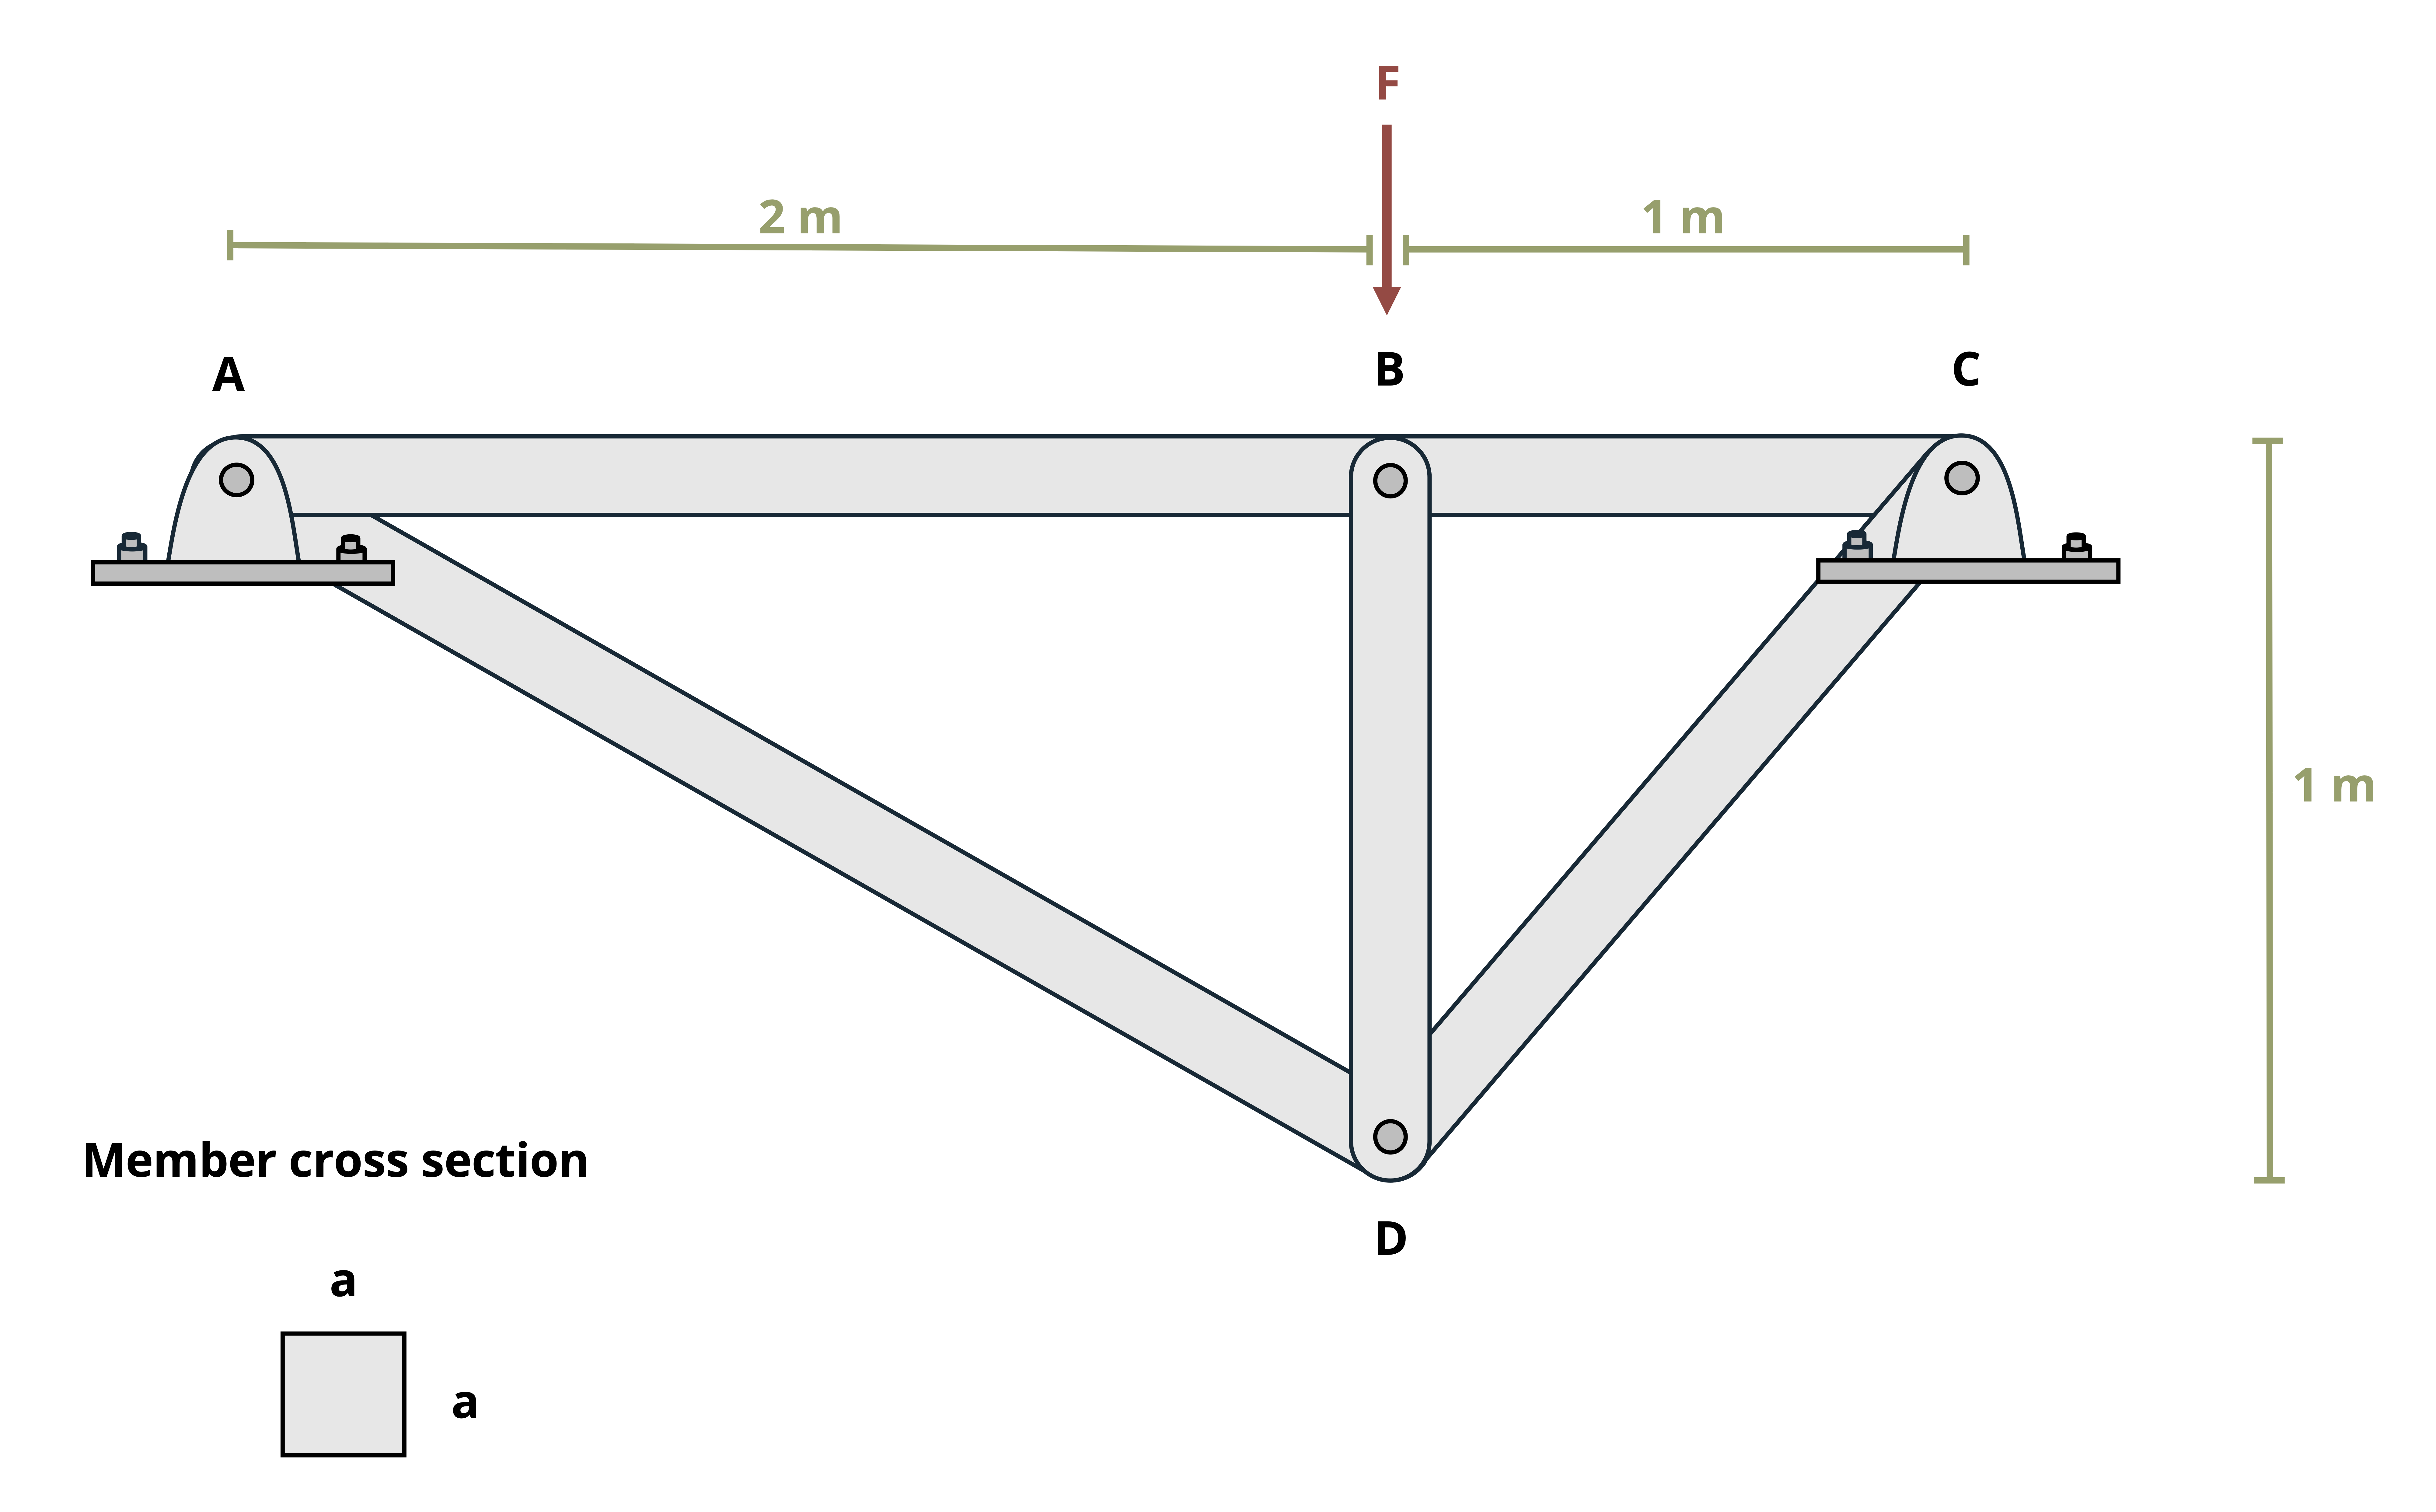
\includegraphics[width=25.16667in,height=\textheight,keepaspectratio]{images/157.png}
{[}Problem adapted from © Kurt Gramoll CC BY NC-SA 4.0{]}

\begin{Shaded}
\begin{Highlighting}[]
\NormalTok{\#| standalone: true}
\NormalTok{\#| viewerHeight: 600}
\NormalTok{\#| components: [viewer]}

\NormalTok{from shiny import App, render, ui, reactive}
\NormalTok{import random}
\NormalTok{import asyncio}
\NormalTok{import io}
\NormalTok{import math}
\NormalTok{import string}
\NormalTok{from datetime import datetime}
\NormalTok{from pathlib import Path}

\NormalTok{def generate\_random\_letters(length):}
\NormalTok{    \# Generate a random string of letters of specified length}
\NormalTok{    return \textquotesingle{}\textquotesingle{}.join(random.choice(string.ascii\_lowercase) for \_ in range(length))  }

\NormalTok{problem\_ID="157"}
\NormalTok{F=reactive.Value("\_\_")}
\NormalTok{FS=reactive.Value("\_\_")}
\NormalTok{σfail=reactive.Value("\_\_")}

\NormalTok{attempts=["Timestamp,Attempt,Answer,Feedback\textbackslash{}n"]}

\NormalTok{app\_ui = ui.page\_fluid(}
\NormalTok{    ui.markdown("**Please enter your ID number from your instructor and click to generate your problem**"),}
\NormalTok{    ui.input\_text("ID","", placeholder="Enter ID Number Here"),}
\NormalTok{    ui.input\_action\_button("generate\_problem", "Generate Problem", class\_="btn{-}primary"),}
\NormalTok{    ui.markdown("**Problem Statement**"),}
\NormalTok{    ui.output\_ui("ui\_problem\_statement"),}
\NormalTok{    ui.input\_text("answer","Your Answer in units of centimeters", placeholder="Please enter your answer"),}
\NormalTok{    ui.input\_action\_button("submit", "Submit Answer", class\_="btn{-}primary"),}
\NormalTok{    ui.download\_button("download", "Download File to Submit", class\_="btn{-}success"),}
\NormalTok{)}


\NormalTok{def server(input, output, session):}
\NormalTok{    \# Initialize a counter for attempts}
\NormalTok{    attempt\_counter = reactive.Value(0)}

\NormalTok{    @output}
\NormalTok{    @render.ui}
\NormalTok{    def ui\_problem\_statement():}
\NormalTok{        return[ui.markdown(f"A small truss is constructed with solid square wood members and subjected to a load of F = \{F()\} kN. Determine the minimum dimension, a, of the member so that the truss will have a factor of safety of \{FS()\}. All members have the same cross{-}section. The wood has a failure stress of σ\textless{}sub\textgreater{}fail\textless{}/sub\textgreater{} = \{σfail()\} MPa.")]}
    
\NormalTok{    @reactive.Effect}
\NormalTok{    @reactive.event(input.generate\_problem)}
\NormalTok{    def randomize\_vars():}
\NormalTok{        random.seed(input.ID())}
\NormalTok{        F.set(random.randrange(15, 50, 1))}
\NormalTok{        FS.set(random.randrange(15, 40, 1)/10)}
\NormalTok{        σfail.set(random.randrange(40, 60, 1))}
        

\NormalTok{    @reactive.Effect}
\NormalTok{    @reactive.event(input.submit)}
\NormalTok{    def \_():}
\NormalTok{        attempt\_counter.set(attempt\_counter() + 1)  \# Increment the attempt counter on each submission.}
    
\NormalTok{        dl = FS()*F()}
\NormalTok{        A = (dl/(σfail()*10**3))*100*100}
\NormalTok{        instr= math.sqrt(A)}
\NormalTok{        if math.isclose(float(input.answer()), instr, rel\_tol=0.01):}
\NormalTok{            check = "*Correct*"}
\NormalTok{            correct\_indicator = "JL"}
\NormalTok{        else:}
\NormalTok{            check = "*Not Correct.*"}
\NormalTok{            correct\_indicator = "JG"}

\NormalTok{        \# Generate random parts for the encoded attempt.}
\NormalTok{        random\_start = generate\_random\_letters(4)}
\NormalTok{        random\_middle = generate\_random\_letters(4)}
\NormalTok{        random\_end = generate\_random\_letters(4)}
\NormalTok{        encoded\_attempt = f"\{random\_start\}\{problem\_ID\}{-}\{random\_middle\}\{attempt\_counter()\}\{correct\_indicator\}{-}\{random\_end\}\{input.ID()\}"}

\NormalTok{        \# Store the most recent encoded attempt in a reactive value so it persists across submissions}
\NormalTok{        session.encoded\_attempt = reactive.Value(encoded\_attempt)}

\NormalTok{        \# Append the attempt data to the attempts list without the encoded attempt}
\NormalTok{        attempts.append(f"\{datetime.now()\}, \{attempt\_counter()\}, \{input.answer()\}, \{check\}\textbackslash{}n")}

\NormalTok{        \# Show feedback to the user.}
\NormalTok{        feedback = ui.markdown(f"Your answer of \{input.answer()\} is \{check\}.")}
\NormalTok{        m = ui.modal(}
\NormalTok{            feedback,}
\NormalTok{            title="Feedback",}
\NormalTok{            easy\_close=True}
\NormalTok{        )}
\NormalTok{        ui.modal\_show(m)}

\NormalTok{    @session.download(filename=lambda: f"Problem\_Log{-}\{problem\_ID\}{-}\{input.ID()\}.csv")}
\NormalTok{    async def download():}
\NormalTok{        \# Start the CSV with the encoded attempt (without label)}
\NormalTok{        final\_encoded = session.encoded\_attempt() if session.encoded\_attempt is not None else "No attempts"}
\NormalTok{        yield f"\{final\_encoded\}\textbackslash{}n\textbackslash{}n"}
        
\NormalTok{        \# Write the header for the remaining CSV data once}
\NormalTok{        yield "Timestamp,Attempt,Answer,Feedback\textbackslash{}n"}
        
\NormalTok{        \# Write the attempts data, ensure that the header from the attempts list is not written again}
\NormalTok{        for attempt in attempts[1:]:  \# Skip the first element which is the header}
\NormalTok{            await asyncio.sleep(0.25)  \# This delay may not be necessary; adjust as needed}
\NormalTok{            yield attempt}


\NormalTok{\# App installation}
\NormalTok{app = App(app\_ui, server)}
\end{Highlighting}
\end{Shaded}

\part{Chapter 5 Problems}

\chapter*{Problem 5.6 - Stress
Concentrations}\label{problem-5.6---stress-concentrations}
\addcontentsline{toc}{chapter}{Problem 5.6 - Stress Concentrations}

\markboth{Problem 5.6 - Stress Concentrations}{Problem 5.6 - Stress
Concentrations}

\pandocbounded{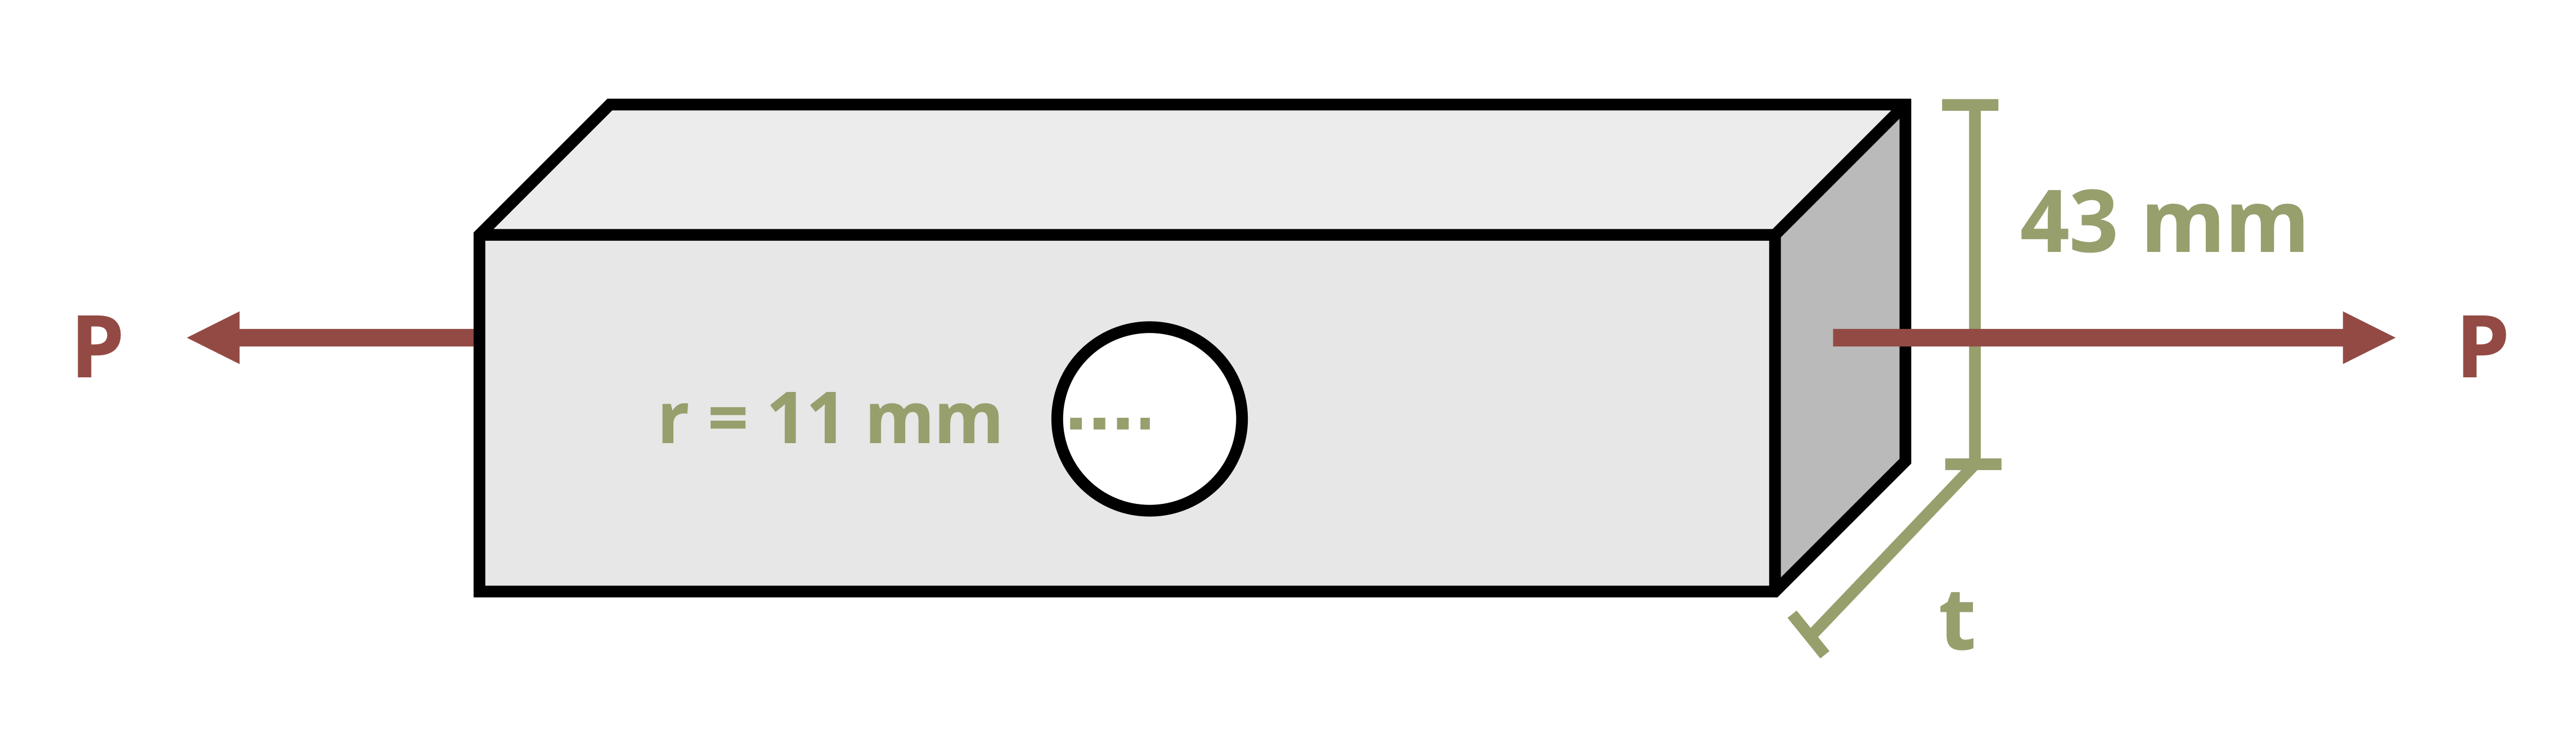
\includegraphics[keepaspectratio]{images/664.png}}
{[}Problem adapted from © Chris Galitz CC BY NC-SA 4.0{]}

\begin{Shaded}
\begin{Highlighting}[]
\NormalTok{\#| standalone: true}
\NormalTok{\#| viewerHeight: 600}
\NormalTok{\#| components: [viewer]}

\NormalTok{from shiny import App, render, ui, reactive}
\NormalTok{import random}
\NormalTok{import asyncio}
\NormalTok{import io}
\NormalTok{import math}
\NormalTok{import string}
\NormalTok{from datetime import datetime}
\NormalTok{from pathlib import Path}

\NormalTok{def generate\_random\_letters(length):}
\NormalTok{    \# Generate a random string of letters of specified length}
\NormalTok{    return \textquotesingle{}\textquotesingle{}.join(random.choice(string.ascii\_lowercase) for \_ in range(length))  }

\NormalTok{problem\_ID="664"}
\NormalTok{t=reactive.Value("\_\_")}
\NormalTok{P=reactive.Value("\_\_")}

\NormalTok{attempts=["Timestamp,Attempt,Answer,Feedback\textbackslash{}n"]}

\NormalTok{app\_ui = ui.page\_fluid(}
\NormalTok{    ui.markdown("**Please enter your ID number from your instructor and click to generate your problem**"),}
\NormalTok{    ui.input\_text("ID","", placeholder="Enter ID Number Here"),}
\NormalTok{    ui.input\_action\_button("generate\_problem", "Generate Problem", class\_="btn{-}primary"),}
\NormalTok{    ui.markdown("**Problem Statement**"),}
\NormalTok{    ui.output\_ui("ui\_problem\_statement"),}
\NormalTok{    ui.input\_text("answer","Your Answer in units of MPa", placeholder="Please enter your answer"),}
\NormalTok{    ui.input\_action\_button("submit", "Submit Answer", class\_="btn{-}primary"),}
\NormalTok{    ui.download\_button("download", "Download File to Submit", class\_="btn{-}success"),}
\NormalTok{)}

\NormalTok{def server(input, output, session):}
\NormalTok{    \# Initialize a counter for attempts}
\NormalTok{    attempt\_counter = reactive.Value(0)}

\NormalTok{    @output}
\NormalTok{    @render.ui}
\NormalTok{    def ui\_problem\_statement():}
\NormalTok{        return[ui.markdown(f"A flat bar of thickness t = \{t()\} mm contains a hole as shown. The bar is subjected to a tensile load P = \{P()\} kN. Determine the maximum tensile stress in the bar.")]}
    
\NormalTok{    @reactive.Effect}
\NormalTok{    @reactive.event(input.generate\_problem)}
\NormalTok{    def randomize\_vars():}
\NormalTok{        random.seed(input.ID())}
\NormalTok{        t.set(random.randrange(10, 25, 1))}
\NormalTok{        P.set(random.randrange(10, 100, 1)/10)}
        
\NormalTok{    @reactive.Effect}
\NormalTok{    @reactive.event(input.submit)}
\NormalTok{    def \_():}
\NormalTok{        attempt\_counter.set(attempt\_counter() + 1)  \# Increment the attempt counter on each submission.}
\NormalTok{        sigma\_norm = P()/(t()*(43{-}22))*1000}
\NormalTok{        instr= 2.15*(sigma\_norm)}
\NormalTok{        if math.isclose(float(input.answer()), instr, rel\_tol=0.1):}
\NormalTok{            check = "*Correct*"}
\NormalTok{            correct\_indicator = "JL"}
\NormalTok{        else:}
\NormalTok{            check = "*Not Correct.*"}
\NormalTok{            correct\_indicator = "JG"}

\NormalTok{        \# Generate random parts for the encoded attempt.}
\NormalTok{        random\_start = generate\_random\_letters(4)}
\NormalTok{        random\_middle = generate\_random\_letters(4)}
\NormalTok{        random\_end = generate\_random\_letters(4)}
\NormalTok{        encoded\_attempt = f"\{random\_start\}\{problem\_ID\}{-}\{random\_middle\}\{attempt\_counter()\}\{correct\_indicator\}{-}\{random\_end\}\{input.ID()\}"}

\NormalTok{        \# Store the most recent encoded attempt in a reactive value so it persists across submissions}
\NormalTok{        session.encoded\_attempt = reactive.Value(encoded\_attempt)}

\NormalTok{        \# Append the attempt data to the attempts list without the encoded attempt}
\NormalTok{        attempts.append(f"\{datetime.now()\}, \{attempt\_counter()\}, \{input.answer()\}, \{check\}\textbackslash{}n")}

\NormalTok{        \# Show feedback to the user.}
\NormalTok{        feedback = ui.markdown(f"Your answer of \{input.answer()\} is \{check\}.")}
\NormalTok{        m = ui.modal(}
\NormalTok{            feedback,}
\NormalTok{            title="Feedback",}
\NormalTok{            easy\_close=True}
\NormalTok{        )}
\NormalTok{        ui.modal\_show(m)}

\NormalTok{    @session.download(filename=lambda: f"Problem\_Log{-}\{problem\_ID\}{-}\{input.ID()\}.csv")}
\NormalTok{    async def download():}
\NormalTok{        \# Start the CSV with the encoded attempt (without label)}
\NormalTok{        final\_encoded = session.encoded\_attempt() if session.encoded\_attempt is not None else "No attempts"}
\NormalTok{        yield f"\{final\_encoded\}\textbackslash{}n\textbackslash{}n"}
        
\NormalTok{        \# Write the header for the remaining CSV data once}
\NormalTok{        yield "Timestamp,Attempt,Answer,Feedback\textbackslash{}n"}
        
\NormalTok{        \# Write the attempts data, ensure that the header from the attempts list is not written again}
\NormalTok{        for attempt in attempts[1:]:  \# Skip the first element which is the header}
\NormalTok{            await asyncio.sleep(0.25)  \# This delay may not be necessary; adjust as needed}
\NormalTok{            yield attempt}

\NormalTok{\# App installation}
\NormalTok{app = App(app\_ui, server)}
\end{Highlighting}
\end{Shaded}

\chapter*{Problem 5.8 - Stress
Concentrations}\label{problem-5.8---stress-concentrations}
\addcontentsline{toc}{chapter}{Problem 5.8 - Stress Concentrations}

\markboth{Problem 5.8 - Stress Concentrations}{Problem 5.8 - Stress
Concentrations}

\begin{figure}[H]

{\centering \pandocbounded{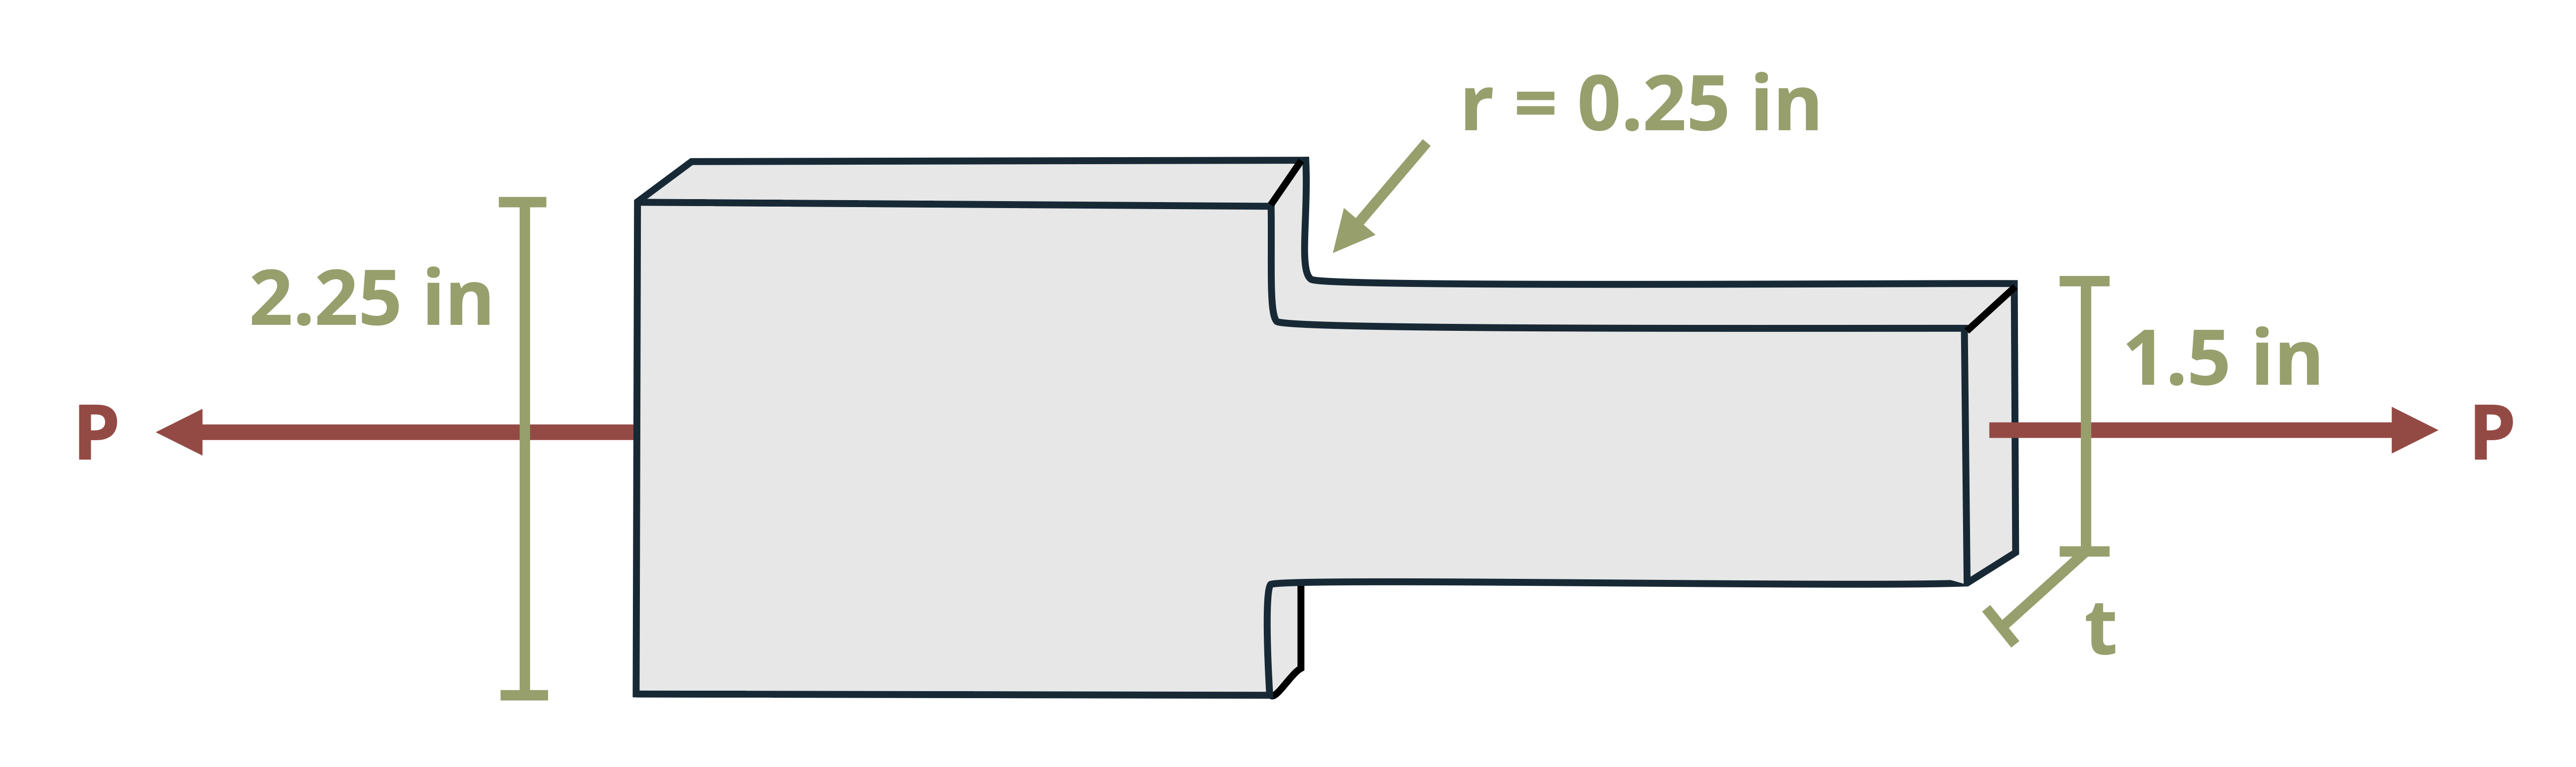
\includegraphics[keepaspectratio]{images/666.png}}

}

\caption{Figure 1: A bar narrows in width.}

\end{figure}%

{[}Problem adapted from © Chris Galitz CC BY NC-SA 4.0{]}

\begin{Shaded}
\begin{Highlighting}[]
\NormalTok{\#| standalone: true}
\NormalTok{\#| viewerHeight: 600}
\NormalTok{\#| components: [viewer]}

\NormalTok{from shiny import App, render, ui, reactive}
\NormalTok{import random}
\NormalTok{import asyncio}
\NormalTok{import io}
\NormalTok{import math}
\NormalTok{import string}
\NormalTok{from datetime import datetime}
\NormalTok{from pathlib import Path}

\NormalTok{def generate\_random\_letters(length):}
\NormalTok{    \# Generate a random string of letters of specified length}
\NormalTok{    return \textquotesingle{}\textquotesingle{}.join(random.choice(string.ascii\_lowercase) for \_ in range(length))  }

\NormalTok{problem\_ID="666"}
\NormalTok{t=reactive.Value("\_\_")}
\NormalTok{P=reactive.Value("\_\_")}

\NormalTok{attempts=["Timestamp,Attempt,Answer,Feedback\textbackslash{}n"]}

\NormalTok{app\_ui = ui.page\_fluid(}
\NormalTok{    ui.markdown("**Please enter your ID number from your instructor and click to generate your problem**"),}
\NormalTok{    ui.input\_text("ID","", placeholder="Enter ID Number Here"),}
\NormalTok{    ui.input\_action\_button("generate\_problem", "Generate Problem", class\_="btn{-}primary"),}
\NormalTok{    ui.markdown("**Problem Statement**"),}
\NormalTok{    ui.output\_ui("ui\_problem\_statement"),}
\NormalTok{    ui.input\_text("answer","Your Answer in units of psi", placeholder="Please enter your answer"),}
\NormalTok{    ui.input\_action\_button("submit", "Submit Answer", class\_="btn{-}primary"),}
\NormalTok{    ui.download\_button("download", "Download File to Submit", class\_="btn{-}success"),}
\NormalTok{)}

\NormalTok{def server(input, output, session):}
\NormalTok{    \# Initialize a counter for attempts}
\NormalTok{    attempt\_counter = reactive.Value(0)}

\NormalTok{    @output}
\NormalTok{    @render.ui}
\NormalTok{    def ui\_problem\_statement():}
\NormalTok{        return[ui.markdown(f"A flat bar of thickness t = \{t()\} in. narrows with fillets as shown. If a load P = \{P()\} lb is applied, determine the maximum stress in the bar.")]}
    
\NormalTok{    @reactive.Effect}
\NormalTok{    @reactive.event(input.generate\_problem)}
\NormalTok{    def randomize\_vars():}
\NormalTok{        random.seed(input.ID())}
\NormalTok{        t.set(random.randrange(10, 100, 5)/100)}
\NormalTok{        P.set(random.randrange(1000, 5000, 100))}
        
\NormalTok{    @reactive.Effect}
\NormalTok{    @reactive.event(input.submit)}
\NormalTok{    def \_():}
\NormalTok{        attempt\_counter.set(attempt\_counter() + 1)  \# Increment the attempt counter on each submission.}
\NormalTok{        sigma\_norm = P()/(t()*(1.5))}
\NormalTok{        instr= 1.95*(sigma\_norm)}
\NormalTok{        if math.isclose(float(input.answer()), instr, rel\_tol=0.1):}
\NormalTok{            check = "*Correct*"}
\NormalTok{            correct\_indicator = "JL"}
\NormalTok{        else:}
\NormalTok{            check = "*Not Correct.*"}
\NormalTok{            correct\_indicator = "JG"}

\NormalTok{        \# Generate random parts for the encoded attempt.}
\NormalTok{        random\_start = generate\_random\_letters(4)}
\NormalTok{        random\_middle = generate\_random\_letters(4)}
\NormalTok{        random\_end = generate\_random\_letters(4)}
\NormalTok{        encoded\_attempt = f"\{random\_start\}\{problem\_ID\}{-}\{random\_middle\}\{attempt\_counter()\}\{correct\_indicator\}{-}\{random\_end\}\{input.ID()\}"}

\NormalTok{        \# Store the most recent encoded attempt in a reactive value so it persists across submissions}
\NormalTok{        session.encoded\_attempt = reactive.Value(encoded\_attempt)}

\NormalTok{        \# Append the attempt data to the attempts list without the encoded attempt}
\NormalTok{        attempts.append(f"\{datetime.now()\}, \{attempt\_counter()\}, \{input.answer()\}, \{check\}\textbackslash{}n")}

\NormalTok{        \# Show feedback to the user.}
\NormalTok{        feedback = ui.markdown(f"Your answer of \{input.answer()\} is \{check\}.")}
\NormalTok{        m = ui.modal(}
\NormalTok{            feedback,}
\NormalTok{            title="Feedback",}
\NormalTok{            easy\_close=True}
\NormalTok{        )}
\NormalTok{        ui.modal\_show(m)}

\NormalTok{    @session.download(filename=lambda: f"Problem\_Log{-}\{problem\_ID\}{-}\{input.ID()\}.csv")}
\NormalTok{    async def download():}
\NormalTok{        \# Start the CSV with the encoded attempt (without label)}
\NormalTok{        final\_encoded = session.encoded\_attempt() if session.encoded\_attempt is not None else "No attempts"}
\NormalTok{        yield f"\{final\_encoded\}\textbackslash{}n\textbackslash{}n"}
        
\NormalTok{        \# Write the header for the remaining CSV data once}
\NormalTok{        yield "Timestamp,Attempt,Answer,Feedback\textbackslash{}n"}
        
\NormalTok{        \# Write the attempts data, ensure that the header from the attempts list is not written again}
\NormalTok{        for attempt in attempts[1:]:  \# Skip the first element which is the header}
\NormalTok{            await asyncio.sleep(0.25)  \# This delay may not be necessary; adjust as needed}
\NormalTok{            yield attempt}

\NormalTok{\# App installation}
\NormalTok{app = App(app\_ui, server)}
\end{Highlighting}
\end{Shaded}

\chapter*{Problem 5.10 - Stress
Concentrations}\label{problem-5.10---stress-concentrations}
\addcontentsline{toc}{chapter}{Problem 5.10 - Stress Concentrations}

\markboth{Problem 5.10 - Stress Concentrations}{Problem 5.10 - Stress
Concentrations}

\begin{figure}[H]

{\centering \pandocbounded{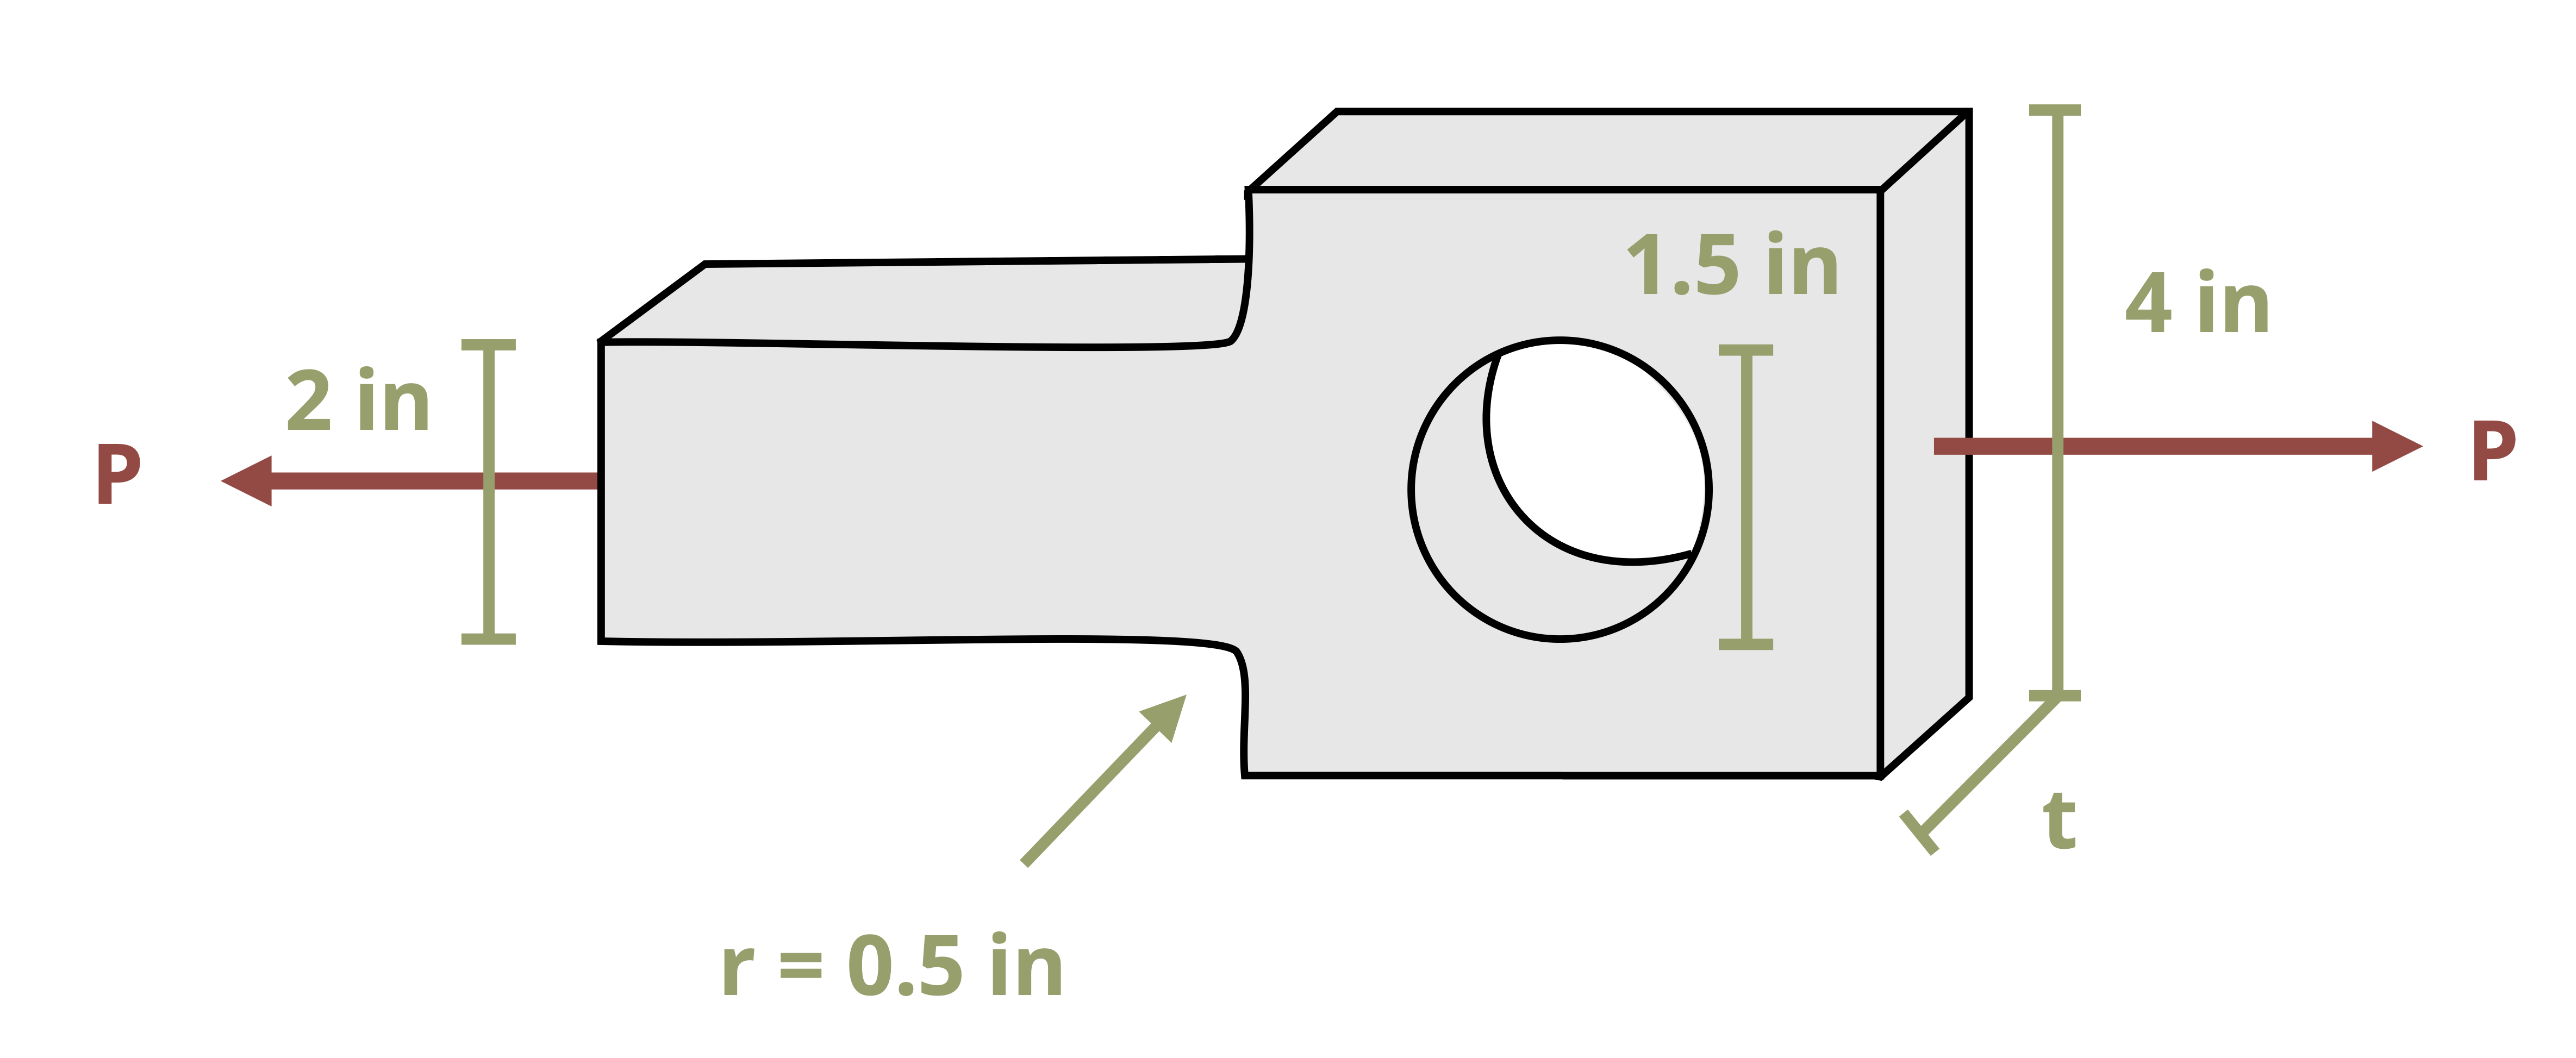
\includegraphics[keepaspectratio]{images/668.png}}

}

\caption{Figure 1: A linkage is subjected to a loading as shown.}

\end{figure}%

{[}Problem adapted from © Chris Galitz CC BY NC-SA 4.0{]}

\begin{Shaded}
\begin{Highlighting}[]
\NormalTok{\#| standalone: true}
\NormalTok{\#| viewerHeight: 600}
\NormalTok{\#| components: [viewer]}

\NormalTok{from shiny import App, render, ui, reactive}
\NormalTok{import random}
\NormalTok{import asyncio}
\NormalTok{import io}
\NormalTok{import math}
\NormalTok{import string}
\NormalTok{from datetime import datetime}
\NormalTok{from pathlib import Path}

\NormalTok{def generate\_random\_letters(length):}
\NormalTok{    \# Generate a random string of letters of specified length}
\NormalTok{    return \textquotesingle{}\textquotesingle{}.join(random.choice(string.ascii\_lowercase) for \_ in range(length))  }

\NormalTok{problem\_ID="668"}
\NormalTok{t=reactive.Value("\_\_")}
\NormalTok{P=reactive.Value("\_\_")}
  
\NormalTok{attempts=["Timestamp,Attempt,Answer,Feedback\textbackslash{}n"]}

\NormalTok{app\_ui = ui.page\_fluid(}
\NormalTok{    ui.markdown("**Please enter your ID number from your instructor and click to generate your problem**"),}
\NormalTok{    ui.input\_text("ID","", placeholder="Enter ID Number Here"),}
\NormalTok{    ui.input\_action\_button("generate\_problem", "Generate Problem", class\_="btn{-}primary"),}
\NormalTok{    ui.markdown("**Problem Statement**"),}
\NormalTok{    ui.output\_ui("ui\_problem\_statement"),}
\NormalTok{    ui.input\_text("answer","Your Answer in units of ksi", placeholder="Please enter your answer"),}
\NormalTok{    ui.input\_action\_button("submit", "Submit Answer", class\_="btn{-}primary"),}
\NormalTok{    ui.download\_button("download", "Download File to Submit", class\_="btn{-}success"),}
\NormalTok{)}

\NormalTok{def server(input, output, session):}
\NormalTok{    \# Initialize a counter for attempts}
\NormalTok{    attempt\_counter = reactive.Value(0)}

\NormalTok{    @output}
\NormalTok{    @render.ui}
\NormalTok{    def ui\_problem\_statement():}
\NormalTok{        return[ui.markdown(f"The linkage of thickness t = \{t()\} in. shown is subjected to load P = \{P()\} kips. Determine the maximum stress in the linkage.")]}
    
\NormalTok{    @reactive.Effect}
\NormalTok{    @reactive.event(input.generate\_problem)}
\NormalTok{    def randomize\_vars():}
\NormalTok{        random.seed(input.ID())}
\NormalTok{        t.set(random.randrange(25, 75, 5)/100)}
\NormalTok{        P.set(random.randrange(20,45,1))}

\NormalTok{    @reactive.Effect}
\NormalTok{    @reactive.event(input.submit)}
\NormalTok{    def \_():}
\NormalTok{        attempt\_counter.set(attempt\_counter() + 1)  \# Increment the attempt counter on each submission.}
\NormalTok{        sigma1 = 1.82*P()/(2*t())}
\NormalTok{        sigma2 = 2.28*P()/(2.5*t())}
\NormalTok{        instr = max(sigma1,sigma2)}
        
\NormalTok{        if math.isclose(float(input.answer()), instr, rel\_tol=0.1):}
\NormalTok{            check = "*Correct*"}
\NormalTok{            correct\_indicator = "JL"}
\NormalTok{        else:}
\NormalTok{            check = "*Not Correct.*"}
\NormalTok{            correct\_indicator = "JG"}

\NormalTok{        \# Generate random parts for the encoded attempt.}
\NormalTok{        random\_start = generate\_random\_letters(4)}
\NormalTok{        random\_middle = generate\_random\_letters(4)}
\NormalTok{        random\_end = generate\_random\_letters(4)}
\NormalTok{        encoded\_attempt = f"\{random\_start\}\{problem\_ID\}{-}\{random\_middle\}\{attempt\_counter()\}\{correct\_indicator\}{-}\{random\_end\}\{input.ID()\}"}

\NormalTok{        \# Store the most recent encoded attempt in a reactive value so it persists across submissions}
\NormalTok{        session.encoded\_attempt = reactive.Value(encoded\_attempt)}

\NormalTok{        \# Append the attempt data to the attempts list without the encoded attempt}
\NormalTok{        attempts.append(f"\{datetime.now()\}, \{attempt\_counter()\}, \{input.answer()\}, \{check\}\textbackslash{}n")}

\NormalTok{        \# Show feedback to the user.}
\NormalTok{        feedback = ui.markdown(f"Your answer of \{input.answer()\} is \{check\}.")}
\NormalTok{        m = ui.modal(}
\NormalTok{            feedback,}
\NormalTok{            title="Feedback",}
\NormalTok{            easy\_close=True}
\NormalTok{        )}
\NormalTok{        ui.modal\_show(m)}

\NormalTok{    @session.download(filename=lambda: f"Problem\_Log{-}\{problem\_ID\}{-}\{input.ID()\}.csv")}
\NormalTok{    async def download():}
\NormalTok{        \# Start the CSV with the encoded attempt (without label)}
\NormalTok{        final\_encoded = session.encoded\_attempt() if session.encoded\_attempt is not None else "No attempts"}
\NormalTok{        yield f"\{final\_encoded\}\textbackslash{}n\textbackslash{}n"}
        
\NormalTok{        \# Write the header for the remaining CSV data once}
\NormalTok{        yield "Timestamp,Attempt,Answer,Feedback\textbackslash{}n"}
        
\NormalTok{        \# Write the attempts data, ensure that the header from the attempts list is not written again}
\NormalTok{        for attempt in attempts[1:]:  \# Skip the first element which is the header}
\NormalTok{            await asyncio.sleep(0.25)  \# This delay may not be necessary; adjust as needed}
\NormalTok{            yield attempt}
            
\NormalTok{\# App installation}
\NormalTok{app = App(app\_ui, server)}
\end{Highlighting}
\end{Shaded}

\chapter*{Problem 5.11 - Axial
Deformation}\label{problem-5.11---axial-deformation}
\addcontentsline{toc}{chapter}{Problem 5.11 - Axial Deformation}

\markboth{Problem 5.11 - Axial Deformation}{Problem 5.11 - Axial
Deformation}

\pandocbounded{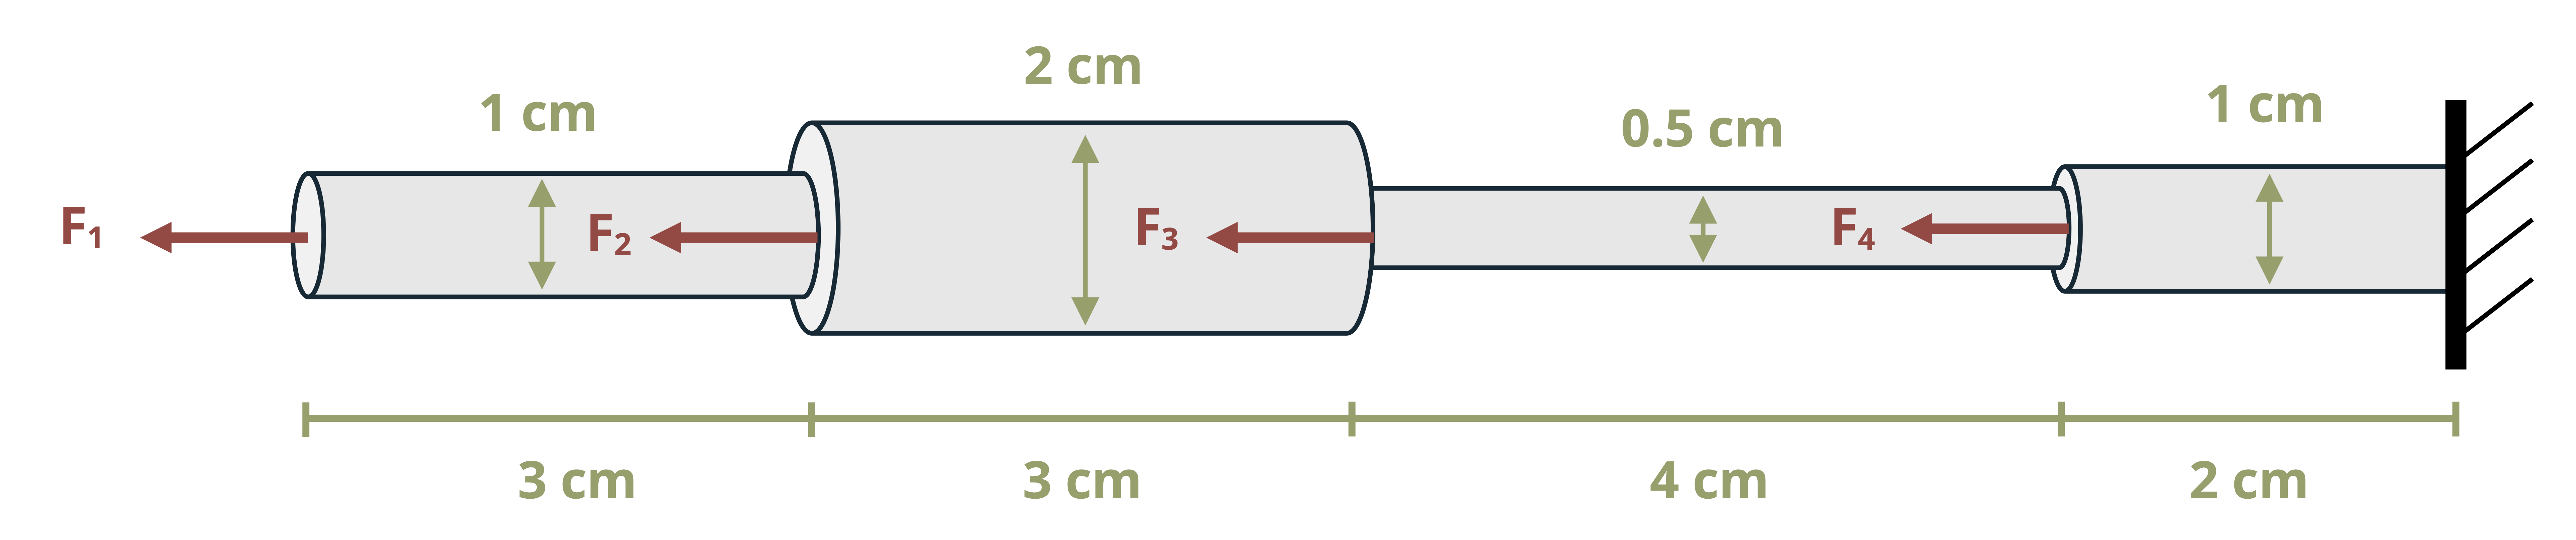
\includegraphics[keepaspectratio]{images/183.png}}
{[}Problem adapted from © Kurt Gramoll CC BY NC-SA 4.0{]}

\begin{Shaded}
\begin{Highlighting}[]
\NormalTok{\#| standalone: true}
\NormalTok{\#| viewerHeight: 600}
\NormalTok{\#| components: [viewer]}

\NormalTok{from shiny import App, render, ui, reactive}
\NormalTok{import random}
\NormalTok{import asyncio}
\NormalTok{import io}
\NormalTok{import math}
\NormalTok{import string}
\NormalTok{from datetime import datetime}
\NormalTok{from pathlib import Path}

\NormalTok{problem\_ID="183"}
\NormalTok{F1=reactive.Value("\_\_")}
\NormalTok{F2=reactive.Value("\_\_")}
\NormalTok{F3=reactive.Value("\_\_")}
\NormalTok{F4=reactive.Value("\_\_")}
\NormalTok{E=210}

\NormalTok{def generate\_random\_letters(length):}
\NormalTok{    \# Generate a random string of letters of specified length}
\NormalTok{    return \textquotesingle{}\textquotesingle{}.join(random.choice(string.ascii\_lowercase) for \_ in range(length))  }

\NormalTok{attempts=["Timestamp,Attempt,Answer,Feedback\textbackslash{}n"]}

\NormalTok{app\_ui = ui.page\_fluid(}
\NormalTok{    ui.markdown("**Please enter your ID number from your instructor and click to generate your problem**"),}
\NormalTok{    ui.input\_text("ID","", placeholder="Enter ID Number Here"),}
\NormalTok{    ui.input\_action\_button("generate\_problem", "Generate Problem", class\_="btn{-}primary"),}
\NormalTok{    ui.markdown("**Problem Statement**"),}
\NormalTok{    ui.output\_ui("ui\_problem\_statement"),}
\NormalTok{    ui.input\_text("answer","Your Answer in units of mm", placeholder="Please enter your answer"),}
\NormalTok{    ui.input\_action\_button("submit", "Submit Answer", class\_="btn{-}primary"),}
\NormalTok{    ui.download\_button("download", "Download File to Submit", class\_="btn{-}success"),}
\NormalTok{)}

\NormalTok{def server(input, output, session):}
\NormalTok{    \# Initialize a counter for attempts}
\NormalTok{    attempt\_counter = reactive.Value(0)}

\NormalTok{    @output}
\NormalTok{    @render.ui}
\NormalTok{    def ui\_problem\_statement():}
\NormalTok{        return[ui.markdown(f"A series of solid, steel, circular bars are loaded with forces as shown, where F\textless{}sub\textgreater{}1\textless{}/sub\textgreater{} = \{F1()\} kN, F\textless{}sub\textgreater{}2\textless{}/sub\textgreater{} = \{F2()\} kN, F\textless{}sub\textgreater{}3\textless{}/sub\textgreater{} = \{F3()\} kN, and F\textless{}sub\textgreater{}4\textless{}/sub\textgreater{} = \{F4()\} kN. What is the total change in length of the system? Assume E = 210 GPa for steel.")]}
    
\NormalTok{    @reactive.Effect}
\NormalTok{    @reactive.event(input.generate\_problem)}
\NormalTok{    def randomize\_vars():}
\NormalTok{        random.seed(input.ID())}
\NormalTok{        F1.set(random.randrange(10, 100, 1)/10)}
\NormalTok{        F2.set(random.randrange(10, 100, 1)/10)}
\NormalTok{        F3.set(random.randrange(10, 100, 1)/10)}
\NormalTok{        F4.set(random.randrange(10, 100, 1)/10)}

\NormalTok{    @reactive.Effect}
\NormalTok{    @reactive.event(input.submit)}
\NormalTok{    def \_():}
\NormalTok{        attempt\_counter.set(attempt\_counter() + 1)  \# Increment the attempt counter on each submission.}
\NormalTok{        instr= ((F1()*3)/(E*math.pi*0.5**2)+((F1()+F2())*3)/(E*math.pi*1**2)+((F1()+F2()+F3())*4)/(E*math.pi*0.25**2)+((F1()+F2()+F3()+F4())*2)/(E*math.pi*0.5**2))/10}
\NormalTok{        if math.isclose(float(input.answer()), instr, rel\_tol=0.01):}
\NormalTok{            check = "*Correct*"}
\NormalTok{            correct\_indicator = "JL"}
\NormalTok{        else:}
\NormalTok{            check = "*Not Correct.*"}
\NormalTok{            correct\_indicator = "JG"}

\NormalTok{        \# Generate random parts for the encoded attempt.}
\NormalTok{        random\_start = generate\_random\_letters(4)}
\NormalTok{        random\_middle = generate\_random\_letters(4)}
\NormalTok{        random\_end = generate\_random\_letters(4)}
\NormalTok{        encoded\_attempt = f"\{random\_start\}\{problem\_ID\}{-}\{random\_middle\}\{attempt\_counter()\}\{correct\_indicator\}{-}\{random\_end\}\{input.ID()\}"}

\NormalTok{        \# Store the most recent encoded attempt in a reactive value so it persists across submissions}
\NormalTok{        session.encoded\_attempt = reactive.Value(encoded\_attempt)}

\NormalTok{        \# Append the attempt data to the attempts list without the encoded attempt}
\NormalTok{        attempts.append(f"\{datetime.now()\}, \{attempt\_counter()\}, \{input.answer()\}, \{check\}\textbackslash{}n")}

\NormalTok{        \# Show feedback to the user.}
\NormalTok{        feedback = ui.markdown(f"Your answer of \{input.answer()\} is \{check\}.")}
\NormalTok{        m = ui.modal(}
\NormalTok{            feedback,}
\NormalTok{            title="Feedback",}
\NormalTok{            easy\_close=True}
\NormalTok{        )}
\NormalTok{        ui.modal\_show(m)}

\NormalTok{    @session.download(filename=lambda: f"Problem\_Log{-}\{problem\_ID\}{-}\{input.ID()\}.csv")}
\NormalTok{    async def download():}
\NormalTok{        \# Start the CSV with the encoded attempt (without label)}
\NormalTok{        final\_encoded = session.encoded\_attempt() if session.encoded\_attempt is not None else "No attempts"}
\NormalTok{        yield f"\{final\_encoded\}\textbackslash{}n\textbackslash{}n"}
        
\NormalTok{        \# Write the header for the remaining CSV data once}
\NormalTok{        yield "Timestamp,Attempt,Answer,Feedback\textbackslash{}n"}
        
\NormalTok{        \# Write the attempts data, ensure that the header from the attempts list is not written again}
\NormalTok{        for attempt in attempts[1:]:  \# Skip the first element which is the header}
\NormalTok{            await asyncio.sleep(0.25)  \# This delay may not be necessary; adjust as needed}
\NormalTok{            yield attempt}

\NormalTok{\# App installation}
\NormalTok{app = App(app\_ui, server)}
\end{Highlighting}
\end{Shaded}

\chapter*{Problem 5.12 - Axial
Deformation}\label{problem-5.12---axial-deformation}
\addcontentsline{toc}{chapter}{Problem 5.12 - Axial Deformation}

\markboth{Problem 5.12 - Axial Deformation}{Problem 5.12 - Axial
Deformation}

\pandocbounded{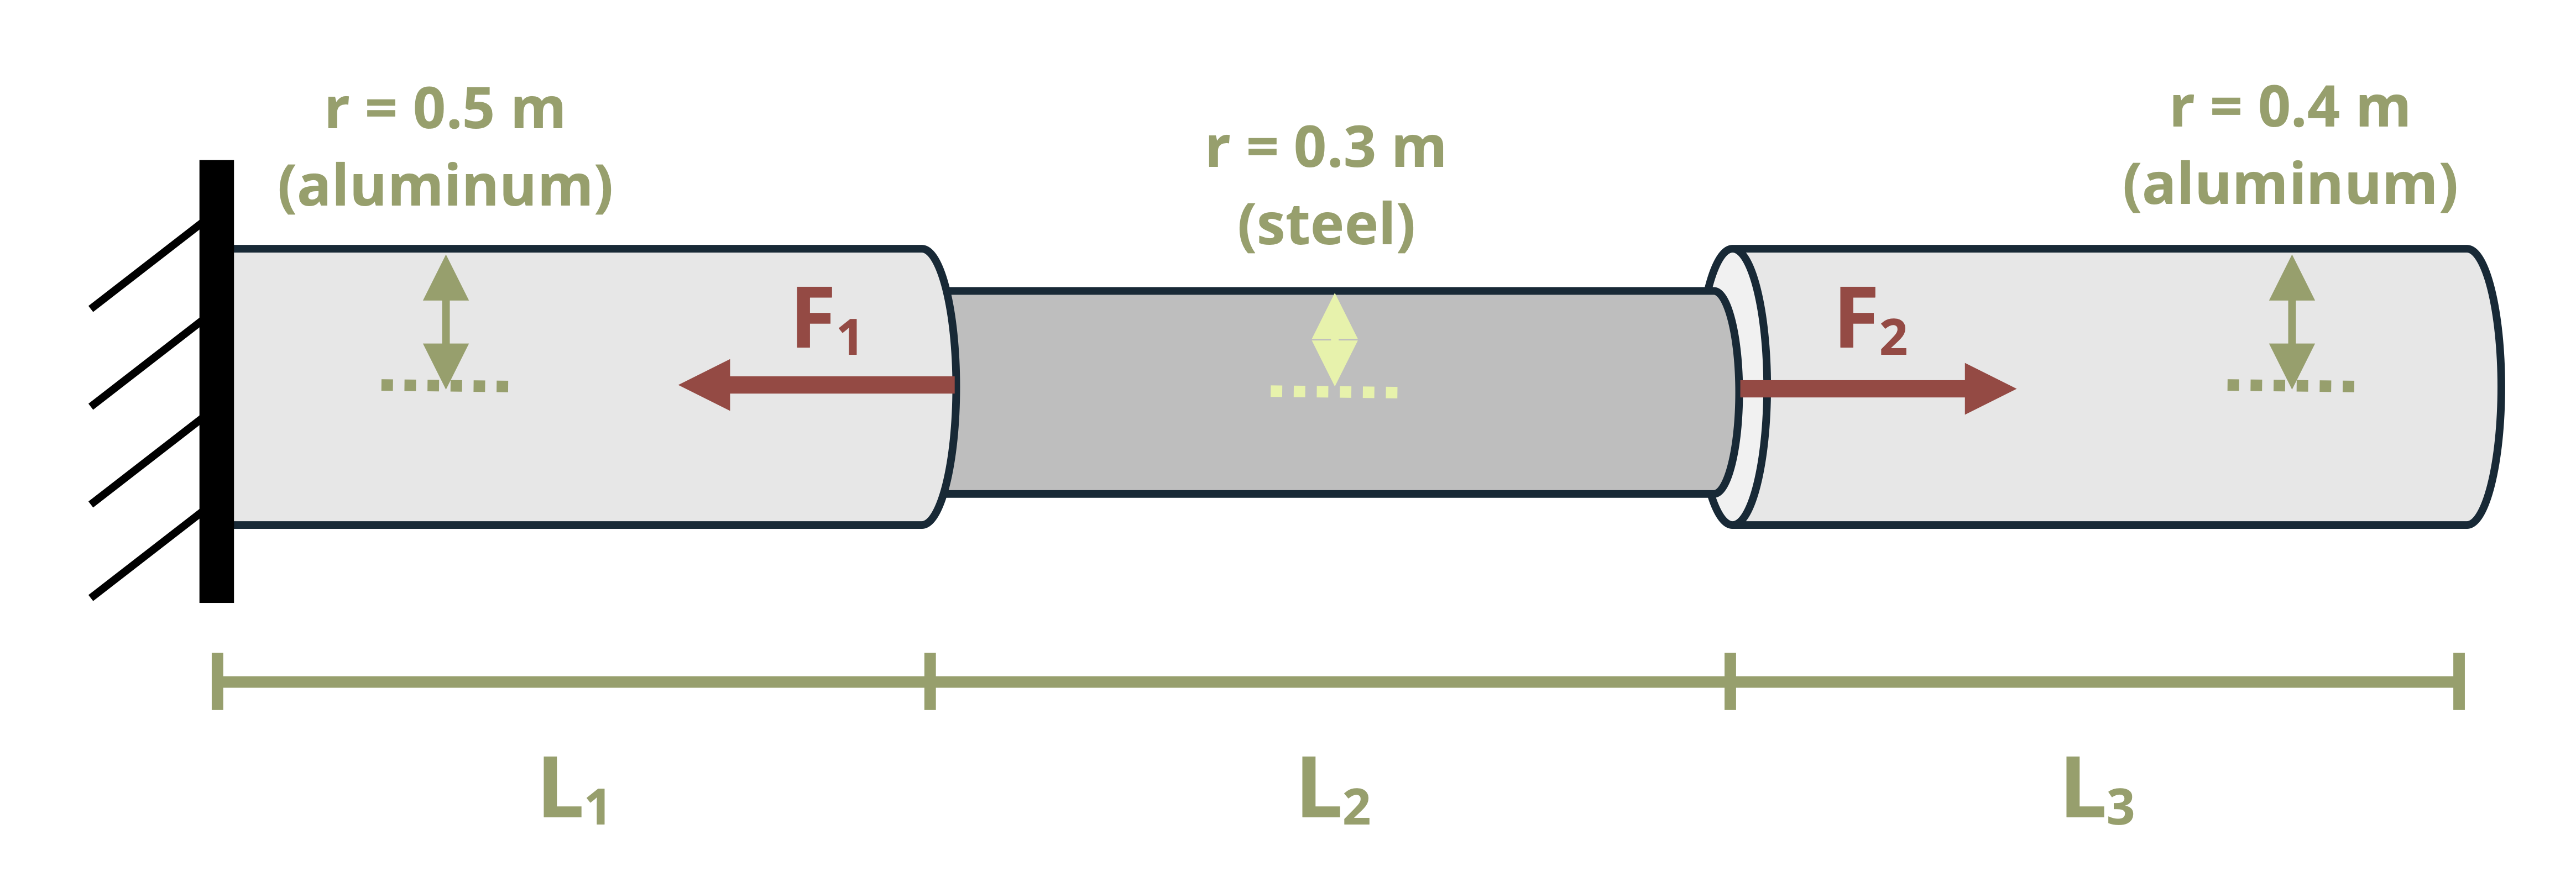
\includegraphics[keepaspectratio]{images/184.png}}
{[}Problem adapted from © Kurt Gramoll CC BY NC-SA 4.0{]}

\begin{Shaded}
\begin{Highlighting}[]
\NormalTok{\#| standalone: true}
\NormalTok{\#| viewerHeight: 600}
\NormalTok{\#| components: [viewer]}

\NormalTok{from shiny import App, render, ui, reactive}
\NormalTok{import random}
\NormalTok{import asyncio}
\NormalTok{import io}
\NormalTok{import math}
\NormalTok{import string}
\NormalTok{from datetime import datetime}
\NormalTok{from pathlib import Path}

\NormalTok{def generate\_random\_letters(length):}
\NormalTok{    \# Generate a random string of letters of specified length}
\NormalTok{    return \textquotesingle{}\textquotesingle{}.join(random.choice(string.ascii\_lowercase) for \_ in range(length)) }

\NormalTok{problem\_ID="184"}
\NormalTok{F1=reactive.Value("\_\_")}
\NormalTok{F2=reactive.Value("\_\_")}
\NormalTok{L1=reactive.Value("\_\_")}
\NormalTok{L2=reactive.Value("\_\_")}
\NormalTok{L3=reactive.Value("\_\_")}
\NormalTok{Esteel = 210}
\NormalTok{Ealuminum = 70}

\NormalTok{attempts=["Timestamp,Attempt,Answer,Feedback\textbackslash{}n"]}

\NormalTok{app\_ui = ui.page\_fluid(}
\NormalTok{    ui.markdown("**Please enter your ID number from your instructor and click to generate your problem**"),}
\NormalTok{    ui.input\_text("ID","", placeholder="Enter ID Number Here"),}
\NormalTok{    ui.input\_action\_button("generate\_problem", "Generate Problem", class\_="btn{-}primary"),}
\NormalTok{    ui.markdown("**Problem Statement**"),}
\NormalTok{    ui.output\_ui("ui\_problem\_statement"),}
\NormalTok{    ui.input\_text("answer","Your Answer in units of micrometers", placeholder="Please enter your answer"),}
\NormalTok{    ui.input\_action\_button("submit", "Submit Answer", class\_="btn{-}primary"),}
\NormalTok{    ui.download\_button("download", "Download File to Submit", class\_="btn{-}success"),}
\NormalTok{)}

\NormalTok{def server(input, output, session):}
\NormalTok{    \# Initialize a counter for attempts}
\NormalTok{    attempt\_counter = reactive.Value(0)}

\NormalTok{    @output}
\NormalTok{    @render.ui}
\NormalTok{    def ui\_problem\_statement():}
\NormalTok{        return[ui.markdown(f"Two forces, F\textless{}sub\textgreater{}1\textless{}/sub\textgreater{} = \{F1()\} kN and F\textless{}sub\textgreater{}2\textless{}/sub\textgreater{} = \{F2()\} kN, are applied to the system of cylinders as shown. If L\textless{}sub\textgreater{}1\textless{}/sub\textgreater{} = \{L1()\} m, L\textless{}sub\textgreater{}2\textless{}/sub\textgreater{} = \{L2()\} m, and L\textless{}sub\textgreater{}3\textless{}/sub\textgreater{} = \{L3()\} m, what is the total change in length of the system? Assume E\textless{}sub\textgreater{}steel\textless{}/sub\textgreater{} = \{Esteel\} GPa and E\textless{}sub\textgreater{}aluminum\textless{}/sub\textgreater{} = \{Ealuminum\} GPa.")]}
    
\NormalTok{    @reactive.Effect}
\NormalTok{    @reactive.event(input.generate\_problem)}
\NormalTok{    def randomize\_vars():}
\NormalTok{        random.seed(input.ID())}
\NormalTok{        F1.set(random.randrange(100, 300, 1)/10)}
\NormalTok{        F2.set(round(F1()/1.5, 2))}
\NormalTok{        L1.set(random.randrange(20, 80, 1)/10)}
\NormalTok{        L2.set(round(L1()*0.6, 2))}
\NormalTok{        L3.set(round(L1()*0.8, 2))}
        
\NormalTok{    @reactive.Effect}
\NormalTok{    @reactive.event(input.submit)}
\NormalTok{    def \_():}
\NormalTok{        attempt\_counter.set(attempt\_counter() + 1)  \# Increment the attempt counter on each submission.}
       
\NormalTok{        instr= ((F2()*10**3*L2())/(math.pi*0.3**2*Esteel*10**9) + ((F2(){-}F1())*1000*L1())/(math.pi*0.5**2*Ealuminum*10**9))*1000000}
\NormalTok{        if math.isclose(float(input.answer()), instr, rel\_tol=0.01):}
\NormalTok{            check = "*Correct*"}
\NormalTok{            correct\_indicator = "JL"}
\NormalTok{        else:}
\NormalTok{            check = "*Not Correct.*"}
\NormalTok{            correct\_indicator = "JG"}

\NormalTok{        \# Generate random parts for the encoded attempt.}
\NormalTok{        random\_start = generate\_random\_letters(4)}
\NormalTok{        random\_middle = generate\_random\_letters(4)}
\NormalTok{        random\_end = generate\_random\_letters(4)}
\NormalTok{        encoded\_attempt = f"\{random\_start\}\{problem\_ID\}{-}\{random\_middle\}\{attempt\_counter()\}\{correct\_indicator\}{-}\{random\_end\}\{input.ID()\}"}

\NormalTok{        \# Store the most recent encoded attempt in a reactive value so it persists across submissions}
\NormalTok{        session.encoded\_attempt = reactive.Value(encoded\_attempt)}

\NormalTok{        \# Append the attempt data to the attempts list without the encoded attempt}
\NormalTok{        attempts.append(f"\{datetime.now()\}, \{attempt\_counter()\}, \{input.answer()\}, \{check\}\textbackslash{}n")}

\NormalTok{        \# Show feedback to the user.}
\NormalTok{        feedback = ui.markdown(f"Your answer of \{input.answer()\} is \{check\}.")}
\NormalTok{        m = ui.modal(}
\NormalTok{            feedback,}
\NormalTok{            title="Feedback",}
\NormalTok{            easy\_close=True}
\NormalTok{        )}
\NormalTok{        ui.modal\_show(m)}

\NormalTok{    @session.download(filename=lambda: f"Problem\_Log{-}\{problem\_ID\}{-}\{input.ID()\}.csv")}
\NormalTok{    async def download():}
\NormalTok{        \# Start the CSV with the encoded attempt (without label)}
\NormalTok{        final\_encoded = session.encoded\_attempt() if session.encoded\_attempt is not None else "No attempts"}
\NormalTok{        yield f"\{final\_encoded\}\textbackslash{}n\textbackslash{}n"}
        
\NormalTok{        \# Write the header for the remaining CSV data once}
\NormalTok{        yield "Timestamp,Attempt,Answer,Feedback\textbackslash{}n"}
        
\NormalTok{        \# Write the attempts data, ensure that the header from the attempts list is not written again}
\NormalTok{        for attempt in attempts[1:]:  \# Skip the first element which is the header}
\NormalTok{            await asyncio.sleep(0.25)  \# This delay may not be necessary; adjust as needed}
\NormalTok{            yield attempt}

\NormalTok{\# App installation}
\NormalTok{app = App(app\_ui, server)}
\end{Highlighting}
\end{Shaded}

\chapter*{Problem 5.13 - Axial
Deformation}\label{problem-5.13---axial-deformation}
\addcontentsline{toc}{chapter}{Problem 5.13 - Axial Deformation}

\markboth{Problem 5.13 - Axial Deformation}{Problem 5.13 - Axial
Deformation}

\pandocbounded{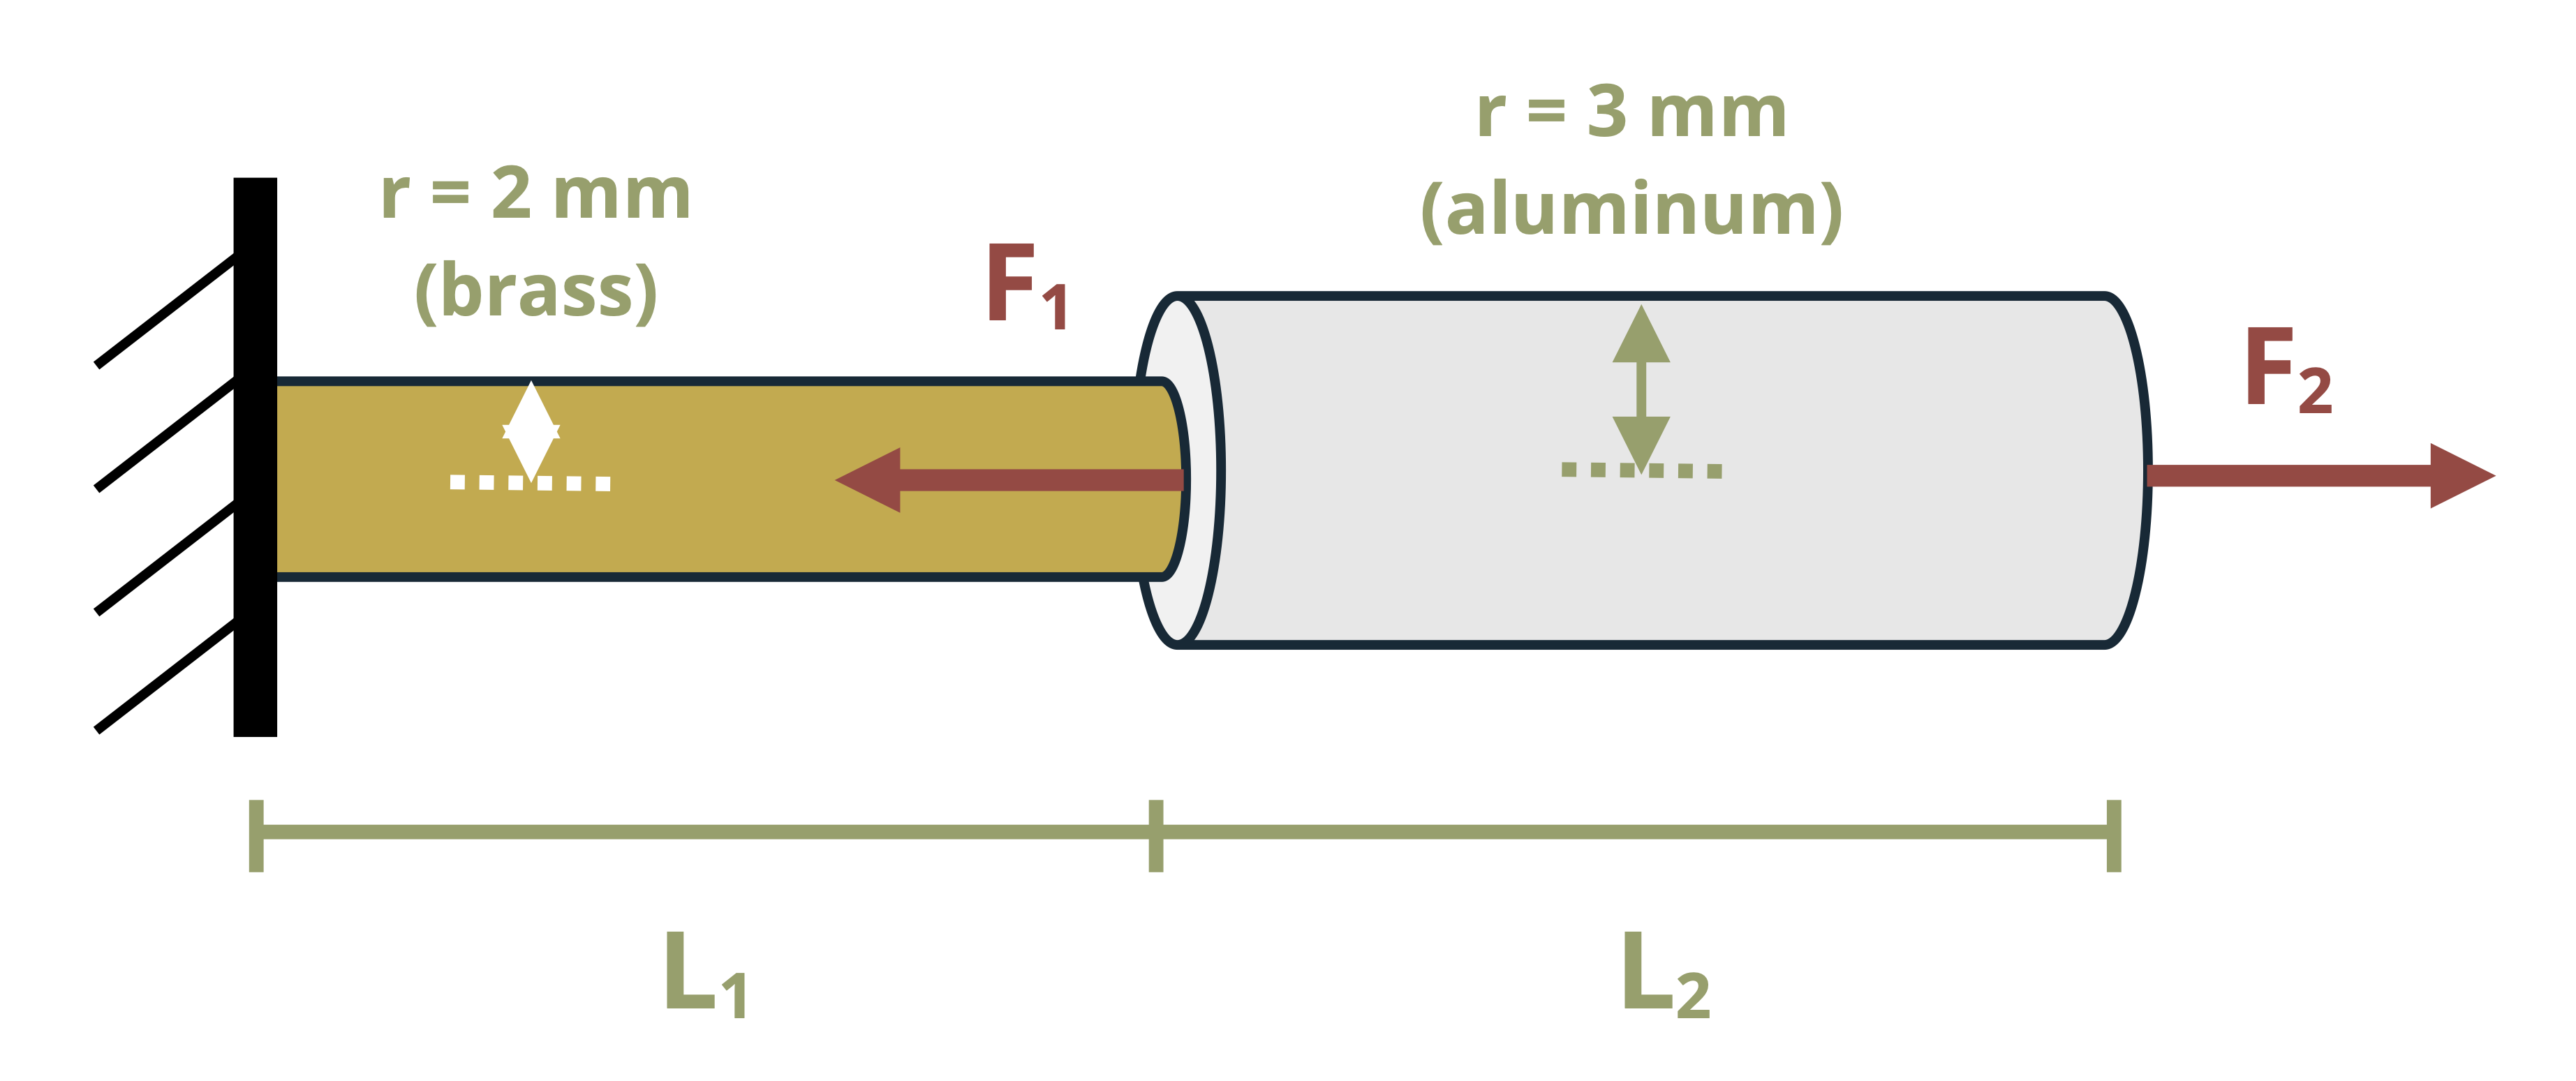
\includegraphics[keepaspectratio]{images/185.png}}
{[}Problem adapted from © Kurt Gramoll CC BY NC-SA 4.0{]}

\begin{Shaded}
\begin{Highlighting}[]
\NormalTok{\#| standalone: true}
\NormalTok{\#| viewerHeight: 600}
\NormalTok{\#| components: [viewer]}

\NormalTok{from shiny import App, render, ui, reactive}
\NormalTok{import random}
\NormalTok{import asyncio}
\NormalTok{import io}
\NormalTok{import math}
\NormalTok{import string}
\NormalTok{from datetime import datetime}
\NormalTok{from pathlib import Path}

\NormalTok{def generate\_random\_letters(length):}
\NormalTok{    \# Generate a random string of letters of specified length}
\NormalTok{    return \textquotesingle{}\textquotesingle{}.join(random.choice(string.ascii\_lowercase) for \_ in range(length))}

\NormalTok{problem\_ID="185"}
\NormalTok{F1=reactive.Value("\_\_")}
\NormalTok{F2=reactive.Value("\_\_")}
\NormalTok{L1=reactive.Value("\_\_")}
\NormalTok{L2=reactive.Value("\_\_")}
\NormalTok{Ebrass = 100}
\NormalTok{Ealuminum = 70}

\NormalTok{attempts=["Timestamp,Attempt,Answer,Feedback\textbackslash{}n"]}

\NormalTok{app\_ui = ui.page\_fluid(}
\NormalTok{    ui.markdown("**Please enter your ID number from your instructor and click to generate your problem**"),}
\NormalTok{    ui.input\_text("ID","", placeholder="Enter ID Number Here"),}
\NormalTok{    ui.input\_action\_button("generate\_problem", "Generate Problem", class\_="btn{-}primary"),}
\NormalTok{    ui.markdown("**Problem Statement**"),}
\NormalTok{    ui.output\_ui("ui\_problem\_statement"),}
\NormalTok{    ui.input\_text("answer","Your Answer in units of mm", placeholder="Please enter your answer"),}
\NormalTok{    ui.input\_action\_button("submit", "Submit Answer", class\_="btn{-}primary"),}
\NormalTok{    ui.download\_button("download", "Download File to Submit", class\_="btn{-}success"),}
\NormalTok{)}

\NormalTok{def server(input, output, session):}
\NormalTok{    \# Initialize a counter for attempts}
\NormalTok{    attempt\_counter = reactive.Value(0)}

\NormalTok{    @output}
\NormalTok{    @render.ui}
\NormalTok{    def ui\_problem\_statement():}
\NormalTok{        return[ui.markdown(f"Two forces, F\textless{}sub\textgreater{}1\textless{}/sub\textgreater{} = \{F1()\} kN and F\textless{}sub\textgreater{}2\textless{}/sub\textgreater{} = \{F2()\} kN, are applied to the system of cylinders as shown. If L\textless{}sub\textgreater{}1\textless{}/sub\textgreater{} = \{L1()\} mm and L\textless{}sub\textgreater{}2\textless{}/sub\textgreater{} = \{L2()\} mm, what is the total change in length of the system. Assume E\textless{}sub\textgreater{}brass\textless{}/sub\textgreater{} = \{Ebrass\} GPa and E\textless{}sub\textgreater{}aluminum\textless{}/sub\textgreater{} = \{Ealuminum\} GPa.")]}
    
\NormalTok{    @reactive.Effect}
\NormalTok{    @reactive.event(input.generate\_problem)}
\NormalTok{    def randomize\_vars():}
\NormalTok{        random.seed(input.ID())}
\NormalTok{        F1.set(random.randrange(10, 100, 1)/10)}
\NormalTok{        F2.set(round(F1()*2, 2))}
\NormalTok{        L1.set(random.randrange(50, 150, 1))}
\NormalTok{        L2.set(round(L1()*1.5))}
        
\NormalTok{    @reactive.Effect}
\NormalTok{    @reactive.event(input.submit)}
\NormalTok{    def \_():}
\NormalTok{        attempt\_counter.set(attempt\_counter() + 1)  \# Increment the attempt counter on each submission.}
\NormalTok{        instr= (((F2(){-}F1())*L1())/(math.pi*.002**2*Ebrass*10**6)) + (F2()*L2())/(math.pi*.003**2*Ealuminum*10**6)}
\NormalTok{        if math.isclose(float(input.answer()), instr, rel\_tol=0.01):}
\NormalTok{            check = "*Correct*"}
\NormalTok{            correct\_indicator = "JL"}
\NormalTok{        else:}
\NormalTok{            check = "*Not Correct.*"}
\NormalTok{            correct\_indicator = "JG"}

\NormalTok{        \# Generate random parts for the encoded attempt.}
\NormalTok{        random\_start = generate\_random\_letters(4)}
\NormalTok{        random\_middle = generate\_random\_letters(4)}
\NormalTok{        random\_end = generate\_random\_letters(4)}
\NormalTok{        encoded\_attempt = f"\{random\_start\}\{problem\_ID\}{-}\{random\_middle\}\{attempt\_counter()\}\{correct\_indicator\}{-}\{random\_end\}\{input.ID()\}"}

\NormalTok{        \# Store the most recent encoded attempt in a reactive value so it persists across submissions}
\NormalTok{        session.encoded\_attempt = reactive.Value(encoded\_attempt)}

\NormalTok{        \# Append the attempt data to the attempts list without the encoded attempt}
\NormalTok{        attempts.append(f"\{datetime.now()\}, \{attempt\_counter()\}, \{input.answer()\}, \{check\}\textbackslash{}n")}

\NormalTok{        \# Show feedback to the user.}
\NormalTok{        feedback = ui.markdown(f"Your answer of \{input.answer()\} is \{check\}.")}
\NormalTok{        m = ui.modal(}
\NormalTok{            feedback,}
\NormalTok{            title="Feedback",}
\NormalTok{            easy\_close=True}
\NormalTok{        )}
\NormalTok{        ui.modal\_show(m)}

\NormalTok{    @session.download(filename=lambda: f"Problem\_Log{-}\{problem\_ID\}{-}\{input.ID()\}.csv")}
\NormalTok{    async def download():}
\NormalTok{        \# Start the CSV with the encoded attempt (without label)}
\NormalTok{        final\_encoded = session.encoded\_attempt() if session.encoded\_attempt is not None else "No attempts"}
\NormalTok{        yield f"\{final\_encoded\}\textbackslash{}n\textbackslash{}n"}
        
\NormalTok{        \# Write the header for the remaining CSV data once}
\NormalTok{        yield "Timestamp,Attempt,Answer,Feedback\textbackslash{}n"}
        
\NormalTok{        \# Write the attempts data, ensure that the header from the attempts list is not written again}
\NormalTok{        for attempt in attempts[1:]:  \# Skip the first element which is the header}
\NormalTok{            await asyncio.sleep(0.25)  \# This delay may not be necessary; adjust as needed}
\NormalTok{            yield attempt}

\NormalTok{\# App installation}
\NormalTok{app = App(app\_ui, server)}
\end{Highlighting}
\end{Shaded}

\chapter*{Problem 5.14 - Axial
Deformation}\label{problem-5.14---axial-deformation}
\addcontentsline{toc}{chapter}{Problem 5.14 - Axial Deformation}

\markboth{Problem 5.14 - Axial Deformation}{Problem 5.14 - Axial
Deformation}

\pandocbounded{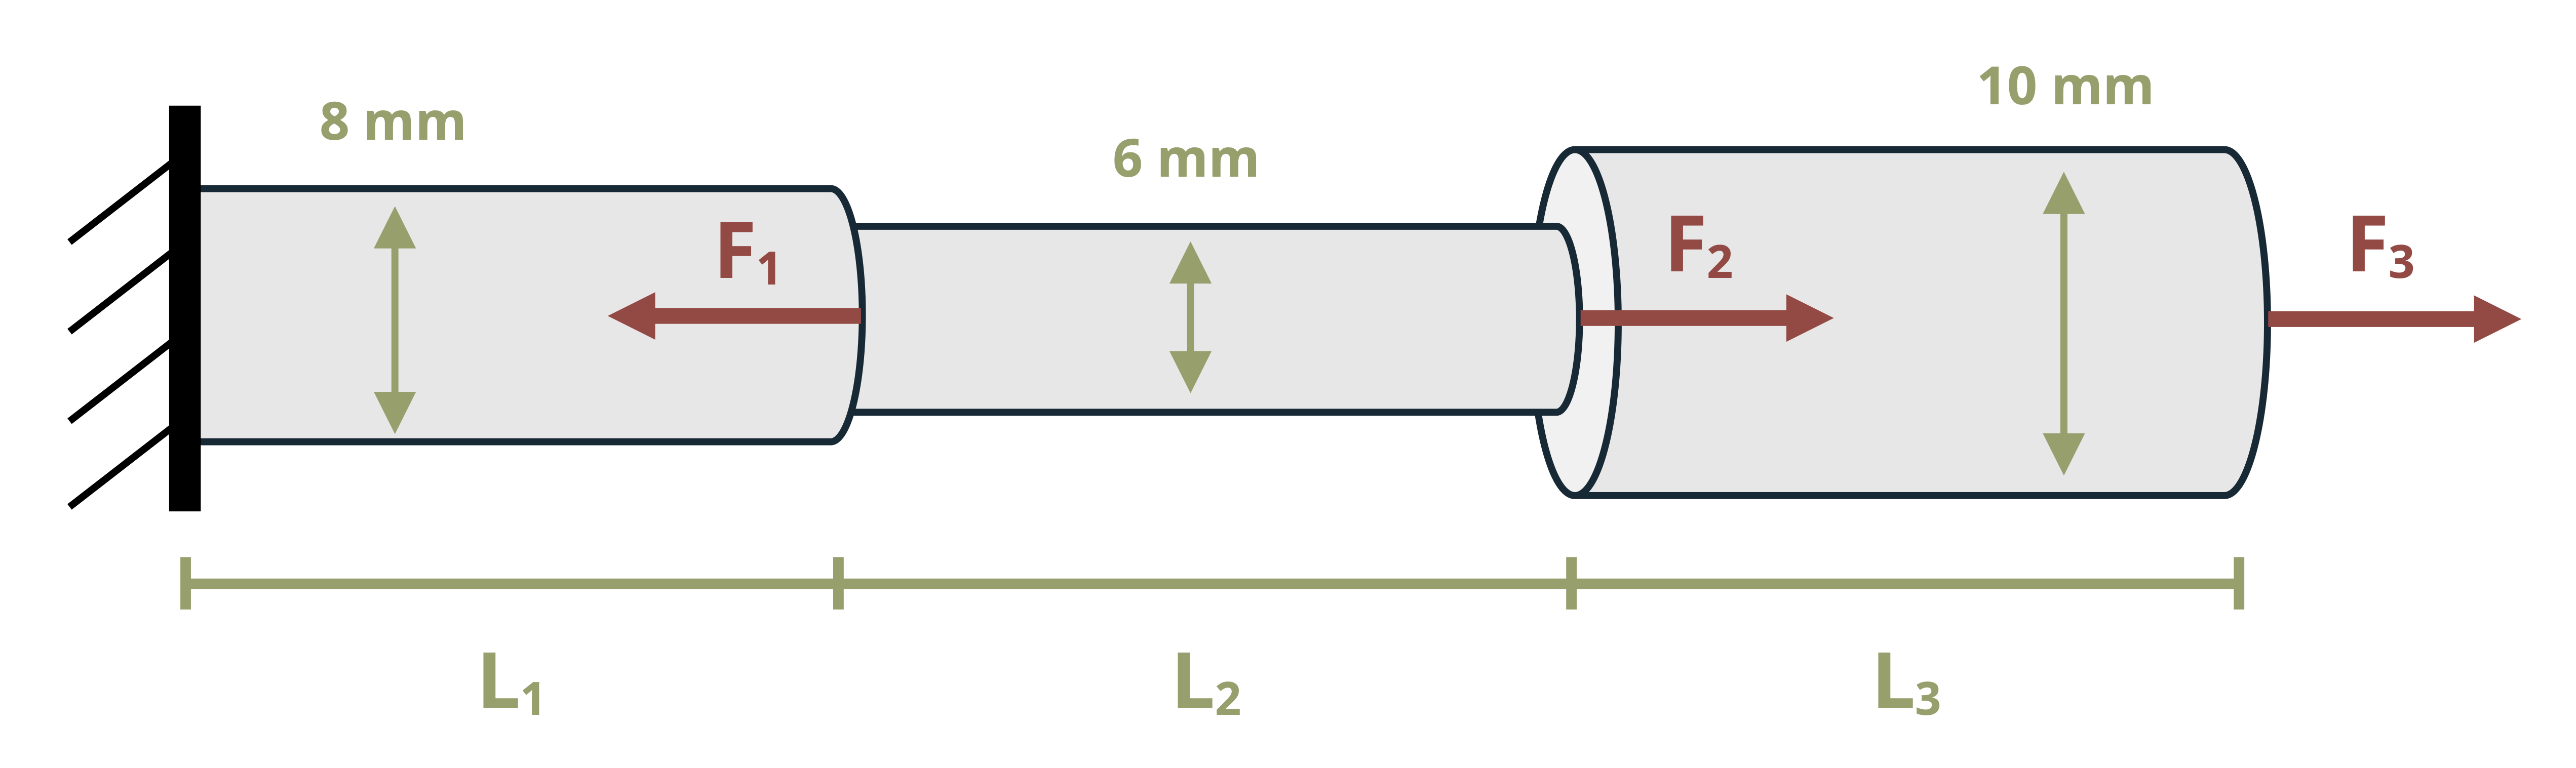
\includegraphics[keepaspectratio]{images/186.png}}
{[}Problem adapted from © Kurt Gramoll CC BY NC-SA 4.0{]}

\begin{Shaded}
\begin{Highlighting}[]
\NormalTok{\#| standalone: true}
\NormalTok{\#| viewerHeight: 600}
\NormalTok{\#| components: [viewer]}

\NormalTok{from shiny import App, render, ui, reactive}
\NormalTok{import random}
\NormalTok{import asyncio}
\NormalTok{import io}
\NormalTok{import math}
\NormalTok{import string}
\NormalTok{from datetime import datetime}
\NormalTok{from pathlib import Path}

\NormalTok{def generate\_random\_letters(length):}
\NormalTok{    \# Generate a random string of letters of specified length}
\NormalTok{    return \textquotesingle{}\textquotesingle{}.join(random.choice(string.ascii\_lowercase) for \_ in range(length))}

\NormalTok{problem\_ID="186"}
\NormalTok{F1=reactive.Value("\_\_")}
\NormalTok{F2=reactive.Value("\_\_")}
\NormalTok{F3=reactive.Value("\_\_")}
\NormalTok{L1=reactive.Value("\_\_")}
\NormalTok{L2=reactive.Value("\_\_")}
\NormalTok{L3=reactive.Value("\_\_")}

\NormalTok{attempts=["Timestamp,Attempt,Answer,Feedback\textbackslash{}n"]}

\NormalTok{app\_ui = ui.page\_fluid(}
\NormalTok{    ui.markdown("**Please enter your ID number from your instructor and click to generate your problem**"),}
\NormalTok{    ui.input\_text("ID","", placeholder="Enter ID Number Here"),}
\NormalTok{    ui.input\_action\_button("generate\_problem", "Generate Problem", class\_="btn{-}primary"),}
\NormalTok{    ui.markdown("**Problem Statement**"),}
\NormalTok{    ui.output\_ui("ui\_problem\_statement"),}
\NormalTok{    ui.input\_text("answer","Your Answer in units of mm", placeholder="Please enter your answer"),}
\NormalTok{    ui.input\_action\_button("submit", "Submit Answer", class\_="btn{-}primary"),}
\NormalTok{    ui.download\_button("download", "Download File to Submit", class\_="btn{-}success"),}
\NormalTok{)}

\NormalTok{def server(input, output, session):}
\NormalTok{    \# Initialize a counter for attempts}
\NormalTok{    attempt\_counter = reactive.Value(0)}

\NormalTok{    @output}
\NormalTok{    @render.ui}
\NormalTok{    def ui\_problem\_statement():}
\NormalTok{        return[ui.markdown(f"A series of solid circular steel bars are loaded as shown, where F\textless{}sub\textgreater{}1\textless{}/sub\textgreater{} = \{F1()\} N, F\textless{}sub\textgreater{}2\textless{}/sub\textgreater{} = \{F2()\} N, and F\textless{}sub\textgreater{}3\textless{}/sub\textgreater{} = \{F3()\} N. If lengths L\textless{}sub\textgreater{}1\textless{}/sub\textgreater{} = L\textless{}sub\textgreater{}2\textless{}/sub\textgreater{} = \{L1()\} cm and L\textless{}sub\textgreater{}3\textless{}/sub\textgreater{} = \{L3()\} cm, determine the total change in length of the system. Assume E\textless{}sub\textgreater{}steel\textless{}/sub\textgreater{} = 210 GPa.")]}
    
\NormalTok{    @reactive.Effect}
\NormalTok{    @reactive.event(input.generate\_problem)}
\NormalTok{    def randomize\_vars():}
\NormalTok{        random.seed(input.ID())}
\NormalTok{        F1.set(random.randrange(20, 100, 1))}
\NormalTok{        F2.set(random.randrange(20, 100, 1))}
\NormalTok{        F3.set(random.randrange(20, 100, 1))}
\NormalTok{        L1.set(random.randrange(20, 60, 1))}
\NormalTok{        L2.set(L1())}
\NormalTok{        L3.set(round(L1()*1.25))}
        
\NormalTok{    @reactive.Effect}
\NormalTok{    @reactive.event(input.submit)}
\NormalTok{    def \_():}
\NormalTok{        attempt\_counter.set(attempt\_counter() + 1)  \# Increment the attempt counter on each submission.}
\NormalTok{        R = F2()+F3(){-}F1()}
\NormalTok{        FBC = F1()+R}
\NormalTok{        dAB = R*L1()/100/(210*10**9*0.004**2*math.pi)}
\NormalTok{        dBC = FBC*L2()/100/(210*10**9*0.003**2*math.pi)}
\NormalTok{        dCD = F3()*L3()/100/(210*10**9*0.005**2*math.pi)}
\NormalTok{        instr= abs((dAB+dBC+dCD)*10**3)}
\NormalTok{        if math.isclose(float(input.answer()), instr, rel\_tol=0.01):}
\NormalTok{            check = "*Correct*"}
\NormalTok{            correct\_indicator = "JL"}
\NormalTok{        else:}
\NormalTok{            check = "*Not Correct.*"}
\NormalTok{            correct\_indicator = "JG"}

\NormalTok{        \# Generate random parts for the encoded attempt.}
\NormalTok{        random\_start = generate\_random\_letters(4)}
\NormalTok{        random\_middle = generate\_random\_letters(4)}
\NormalTok{        random\_end = generate\_random\_letters(4)}
\NormalTok{        encoded\_attempt = f"\{random\_start\}\{problem\_ID\}{-}\{random\_middle\}\{attempt\_counter()\}\{correct\_indicator\}{-}\{random\_end\}\{input.ID()\}"}

\NormalTok{        \# Store the most recent encoded attempt in a reactive value so it persists across submissions}
\NormalTok{        session.encoded\_attempt = reactive.Value(encoded\_attempt)}

\NormalTok{        \# Append the attempt data to the attempts list without the encoded attempt}
\NormalTok{        attempts.append(f"\{datetime.now()\}, \{attempt\_counter()\}, \{input.answer()\}, \{check\}\textbackslash{}n")}

\NormalTok{        \# Show feedback to the user.}
\NormalTok{        feedback = ui.markdown(f"Your answer of \{input.answer()\} is \{check\}.")}
\NormalTok{        m = ui.modal(}
\NormalTok{            feedback,}
\NormalTok{            title="Feedback",}
\NormalTok{            easy\_close=True}
\NormalTok{        )}
\NormalTok{        ui.modal\_show(m)}

\NormalTok{    @session.download(filename=lambda: f"Problem\_Log{-}\{problem\_ID\}{-}\{input.ID()\}.csv")}
\NormalTok{    async def download():}
\NormalTok{        \# Start the CSV with the encoded attempt (without label)}
\NormalTok{        final\_encoded = session.encoded\_attempt() if session.encoded\_attempt is not None else "No attempts"}
\NormalTok{        yield f"\{final\_encoded\}\textbackslash{}n\textbackslash{}n"}
        
\NormalTok{        \# Write the header for the remaining CSV data once}
\NormalTok{        yield "Timestamp,Attempt,Answer,Feedback\textbackslash{}n"}
        
\NormalTok{        \# Write the attempts data, ensure that the header from the attempts list is not written again}
\NormalTok{        for attempt in attempts[1:]:  \# Skip the first element which is the header}
\NormalTok{            await asyncio.sleep(0.25)  \# This delay may not be necessary; adjust as needed}
\NormalTok{            yield attempt}

\NormalTok{\# App installation}
\NormalTok{app = App(app\_ui, server)}
\end{Highlighting}
\end{Shaded}

\chapter*{Problem 5.15 - Axial
Deformation}\label{problem-5.15---axial-deformation}
\addcontentsline{toc}{chapter}{Problem 5.15 - Axial Deformation}

\markboth{Problem 5.15 - Axial Deformation}{Problem 5.15 - Axial
Deformation}

\pandocbounded{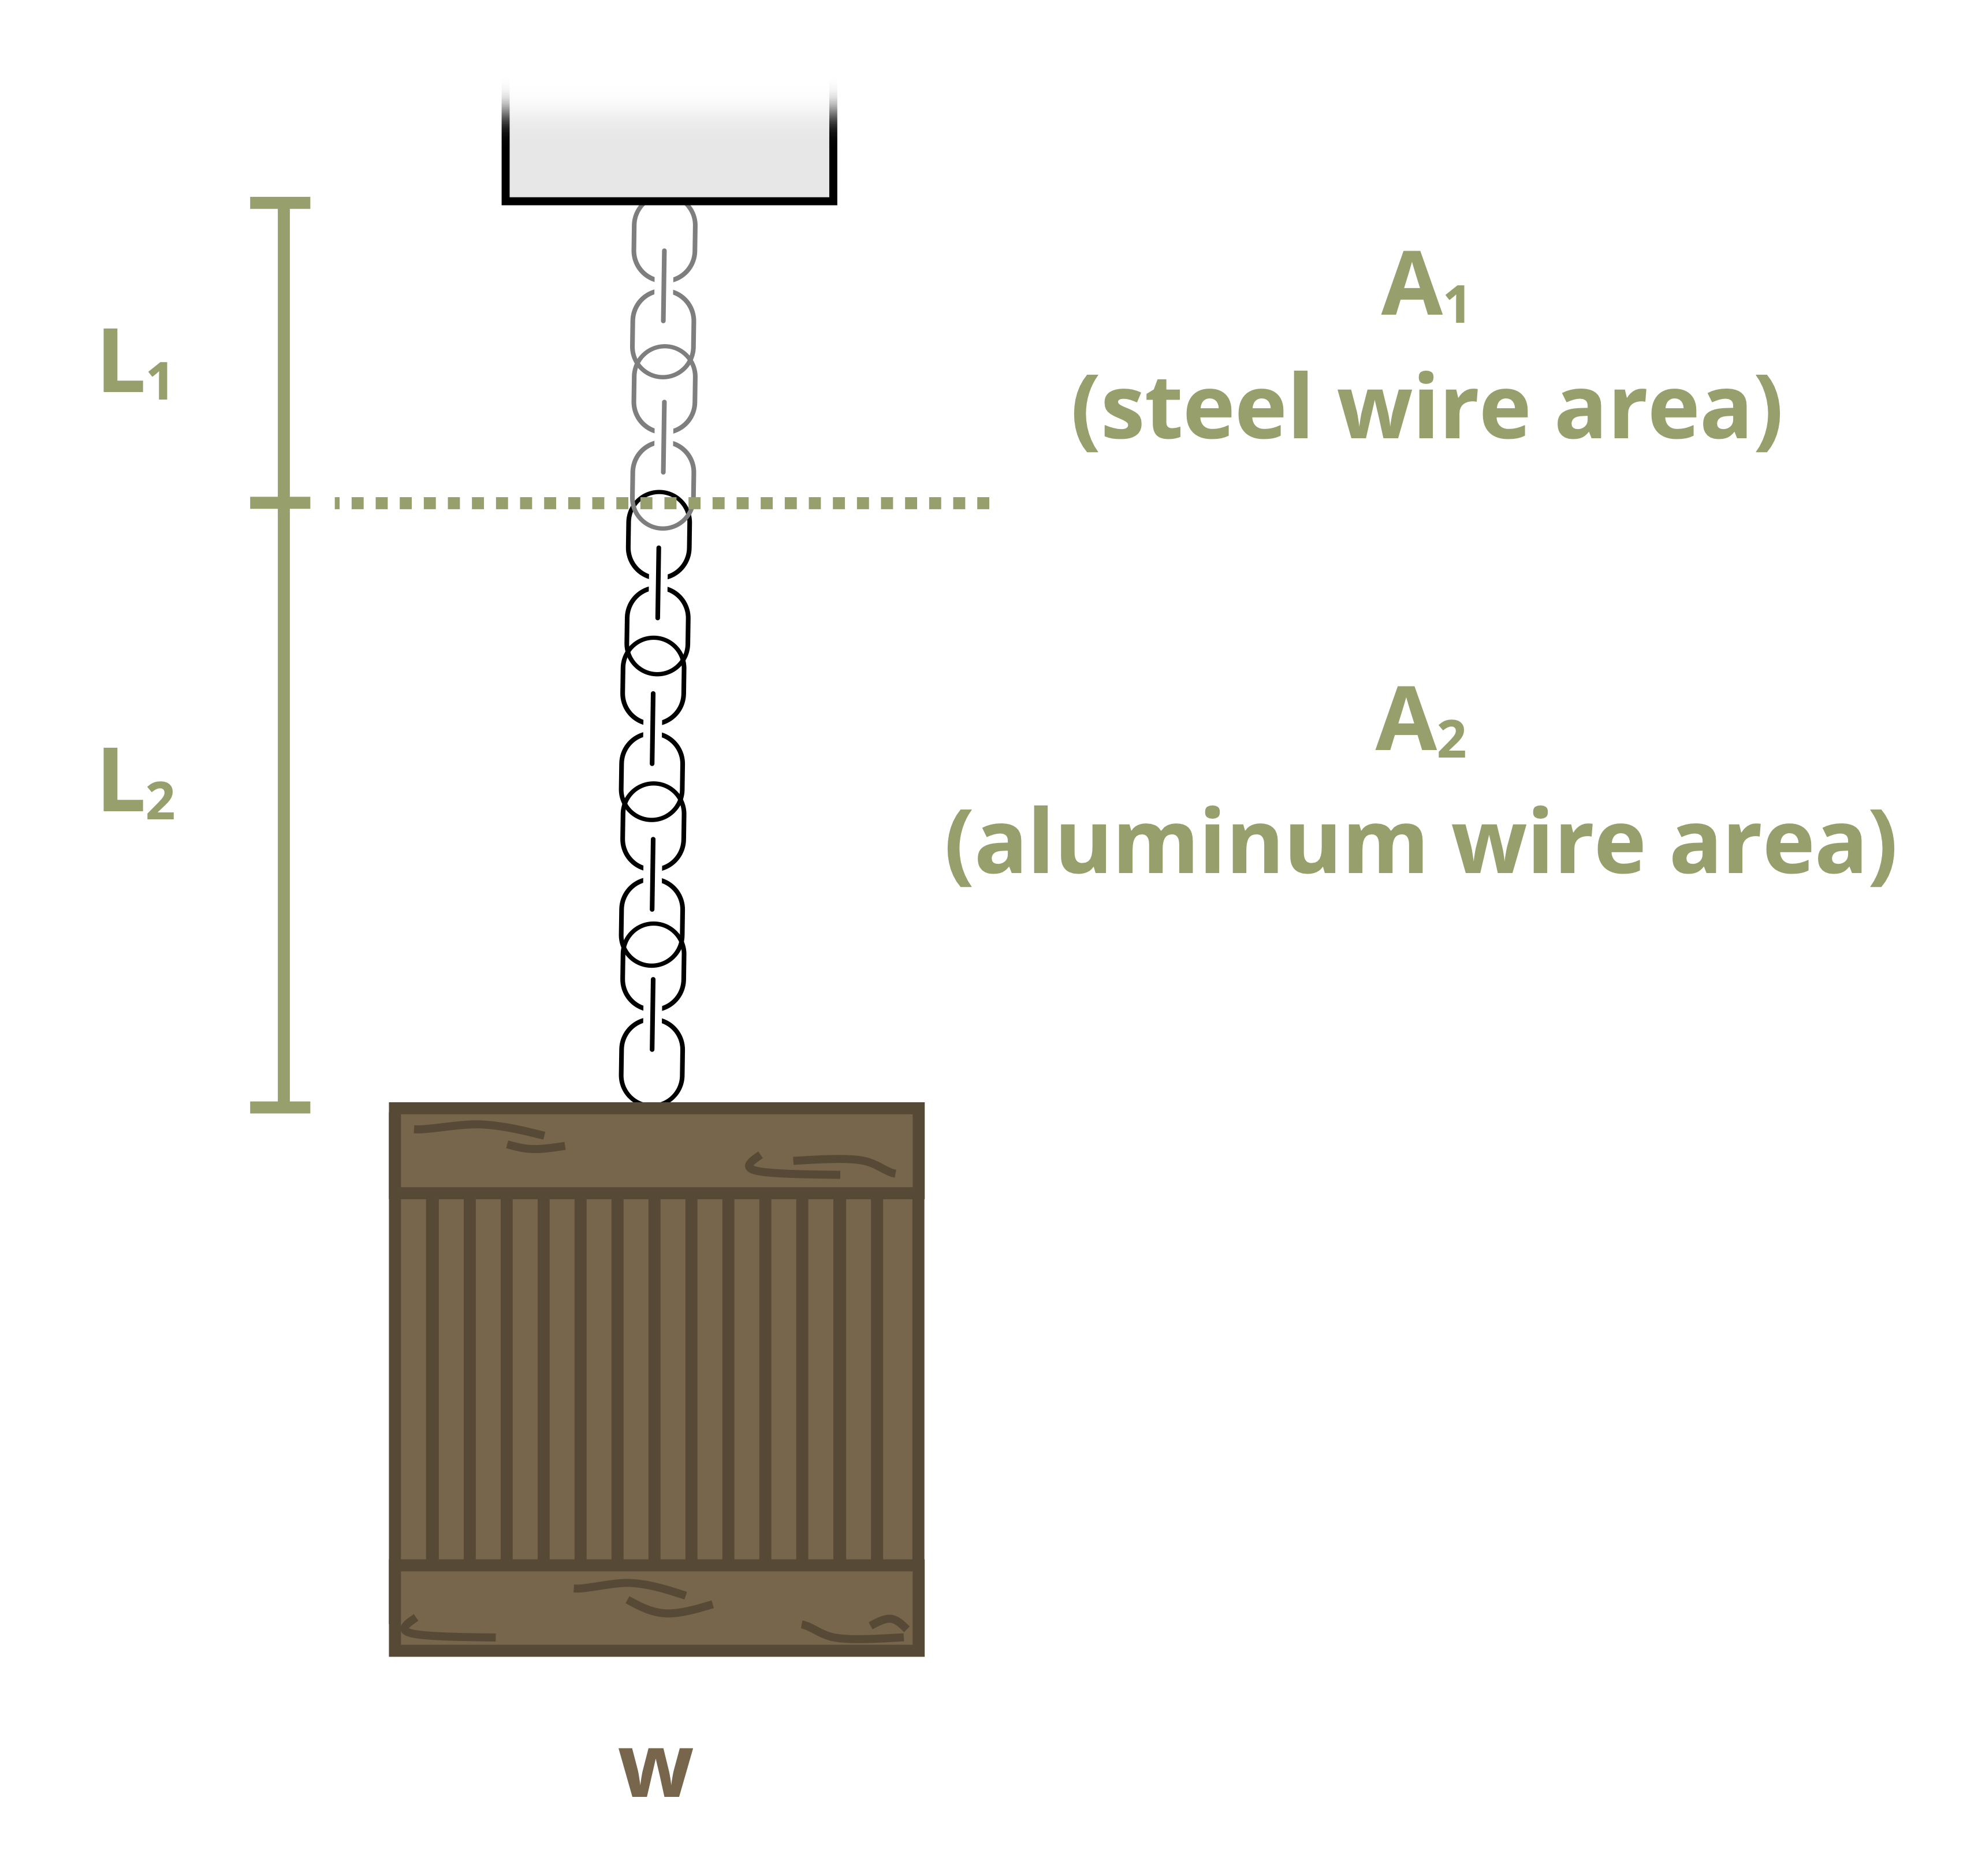
\includegraphics[keepaspectratio]{images/187.png}}
{[}Problem adapted from © Kurt Gramoll CC BY NC-SA 4.0{]}

\begin{Shaded}
\begin{Highlighting}[]
\NormalTok{\#| standalone: true}
\NormalTok{\#| viewerHeight: 600}
\NormalTok{\#| components: [viewer]}

\NormalTok{from shiny import App, render, ui, reactive}
\NormalTok{import random}
\NormalTok{import asyncio}
\NormalTok{import io}
\NormalTok{import math}
\NormalTok{import string}
\NormalTok{from datetime import datetime}
\NormalTok{from pathlib import Path}

\NormalTok{def generate\_random\_letters(length):}
\NormalTok{    \# Generate a random string of letters of specified length}
\NormalTok{    return \textquotesingle{}\textquotesingle{}.join(random.choice(string.ascii\_lowercase) for \_ in range(length)) }

\NormalTok{problem\_ID="187"}
\NormalTok{W=reactive.Value("\_\_")}
\NormalTok{L1=reactive.Value("\_\_")}
\NormalTok{L2=reactive.Value("\_\_")}
\NormalTok{A1=reactive.Value("\_\_")}
\NormalTok{A2=reactive.Value("\_\_")}
\NormalTok{Esteel = 29000}
\NormalTok{Ealuminum = 10000}

\NormalTok{attempts=["Timestamp,Attempt,Answer,Feedback\textbackslash{}n"]}

\NormalTok{app\_ui = ui.page\_fluid(}
\NormalTok{    ui.markdown("**Please enter your ID number from your instructor and click to generate your problem**"),}
\NormalTok{    ui.input\_text("ID","", placeholder="Enter ID Number Here"),}
\NormalTok{    ui.input\_action\_button("generate\_problem", "Generate Problem", class\_="btn{-}primary"),}
\NormalTok{    ui.markdown("**Problem Statement**"),}
\NormalTok{    ui.output\_ui("ui\_problem\_statement"),}
\NormalTok{    ui.input\_text("answer","Your Answer in units of inches", placeholder="Please enter your answer"),}
\NormalTok{    ui.input\_action\_button("submit", "Submit Answer", class\_="btn{-}primary"),}
\NormalTok{    ui.download\_button("download", "Download File to Submit", class\_="btn{-}success"),}
\NormalTok{)}

\NormalTok{def server(input, output, session):}
\NormalTok{    \# Initialize a counter for attempts}
\NormalTok{    attempt\_counter = reactive.Value(0)}

\NormalTok{    @output}
\NormalTok{    @render.ui}
\NormalTok{    def ui\_problem\_statement():}
\NormalTok{        return[ui.markdown(f"A crate weight W = \{W()\} lb is attached to a cable constructed from steel of length L\textless{}sub\textgreater{}1\textless{}/sub\textgreater{} = \{L1()\} in. and Area A\textless{}sub\textgreater{}1\textless{}/sub\textgreater{} = \{A1()\} in.\textless{}sup\textgreater{}2\textless{}/sup\textgreater{} and aluminum of length L\textless{}sub\textgreater{}2\textless{}/sub\textgreater{} = \{L2()\} in. and area A\textless{}sub\textgreater{}2\textless{}/sub\textgreater{} = \{A2()\} in.\textless{}sup\textgreater{}2\textless{}/sup\textgreater{}. What is the total deflection of the crate after it is attached to the wire? Assume E\textless{}sub\textgreater{}steel\textless{}/sub\textgreater{} = \{Esteel\} ksi and E\textless{}sub\textgreater{}aluminum\textless{}/sub\textgreater{} = \{Ealuminum\} ksi. Neglect the weight of the wires.")]}
    
\NormalTok{    @reactive.Effect}
\NormalTok{    @reactive.event(input.generate\_problem)}
\NormalTok{    def randomize\_vars():}
\NormalTok{        random.seed(input.ID())}
\NormalTok{        W.set(random.randrange(50, 250, 1))}
\NormalTok{        L1.set(random.randrange(10, 30, 1))}
\NormalTok{        L2.set(round(L1()*2, 2))}
\NormalTok{        A1.set(random.randrange(1, 5, 1)/100)}
\NormalTok{        A2.set(random.randrange(1, 5, 1)/100)}
        
\NormalTok{    @reactive.Effect}
\NormalTok{    @reactive.event(input.submit)}
\NormalTok{    def \_():}
\NormalTok{        attempt\_counter.set(attempt\_counter() + 1)  \# Increment the attempt counter on each submission.}
        
\NormalTok{        instr=(W()*L1()/(A1()*Esteel*1000) + (W()*L2()/(A2()*Ealuminum*1000)))}
\NormalTok{        if math.isclose(float(input.answer()), instr, rel\_tol=0.01):}
\NormalTok{            check = "*Correct*"}
\NormalTok{            correct\_indicator = "JL"}
\NormalTok{        else:}
\NormalTok{            check = "*Not Correct.*"}
\NormalTok{            correct\_indicator = "JG"}

\NormalTok{        \# Generate random parts for the encoded attempt.}
\NormalTok{        random\_start = generate\_random\_letters(4)}
\NormalTok{        random\_middle = generate\_random\_letters(4)}
\NormalTok{        random\_end = generate\_random\_letters(4)}
\NormalTok{        encoded\_attempt = f"\{random\_start\}\{problem\_ID\}{-}\{random\_middle\}\{attempt\_counter()\}\{correct\_indicator\}{-}\{random\_end\}\{input.ID()\}"}

\NormalTok{        \# Store the most recent encoded attempt in a reactive value so it persists across submissions}
\NormalTok{        session.encoded\_attempt = reactive.Value(encoded\_attempt)}

\NormalTok{        \# Append the attempt data to the attempts list without the encoded attempt}
\NormalTok{        attempts.append(f"\{datetime.now()\}, \{attempt\_counter()\}, \{input.answer()\}, \{check\}\textbackslash{}n")}

\NormalTok{        \# Show feedback to the user.}
\NormalTok{        feedback = ui.markdown(f"Your answer of \{input.answer()\} is \{check\}.")}
\NormalTok{        m = ui.modal(}
\NormalTok{            feedback,}
\NormalTok{            title="Feedback",}
\NormalTok{            easy\_close=True}
\NormalTok{        )}
\NormalTok{        ui.modal\_show(m)}

\NormalTok{    @session.download(filename=lambda: f"Problem\_Log{-}\{problem\_ID\}{-}\{input.ID()\}.csv")}
\NormalTok{    async def download():}
\NormalTok{        \# Start the CSV with the encoded attempt (without label)}
\NormalTok{        final\_encoded = session.encoded\_attempt() if session.encoded\_attempt is not None else "No attempts"}
\NormalTok{        yield f"\{final\_encoded\}\textbackslash{}n\textbackslash{}n"}
        
\NormalTok{        \# Write the header for the remaining CSV data once}
\NormalTok{        yield "Timestamp,Attempt,Answer,Feedback\textbackslash{}n"}
        
\NormalTok{        \# Write the attempts data, ensure that the header from the attempts list is not written again}
\NormalTok{        for attempt in attempts[1:]:  \# Skip the first element which is the header}
\NormalTok{            await asyncio.sleep(0.25)  \# This delay may not be necessary; adjust as needed}
\NormalTok{            yield attempt}

\NormalTok{\# App installation}
\NormalTok{app = App(app\_ui, server)}
\end{Highlighting}
\end{Shaded}

\chapter*{Problem 5.27 - Deformation in Systems of
Bars}\label{problem-5.27---deformation-in-systems-of-bars}
\addcontentsline{toc}{chapter}{Problem 5.27 - Deformation in Systems of
Bars}

\markboth{Problem 5.27 - Deformation in Systems of Bars}{Problem 5.27 -
Deformation in Systems of Bars}

\pandocbounded{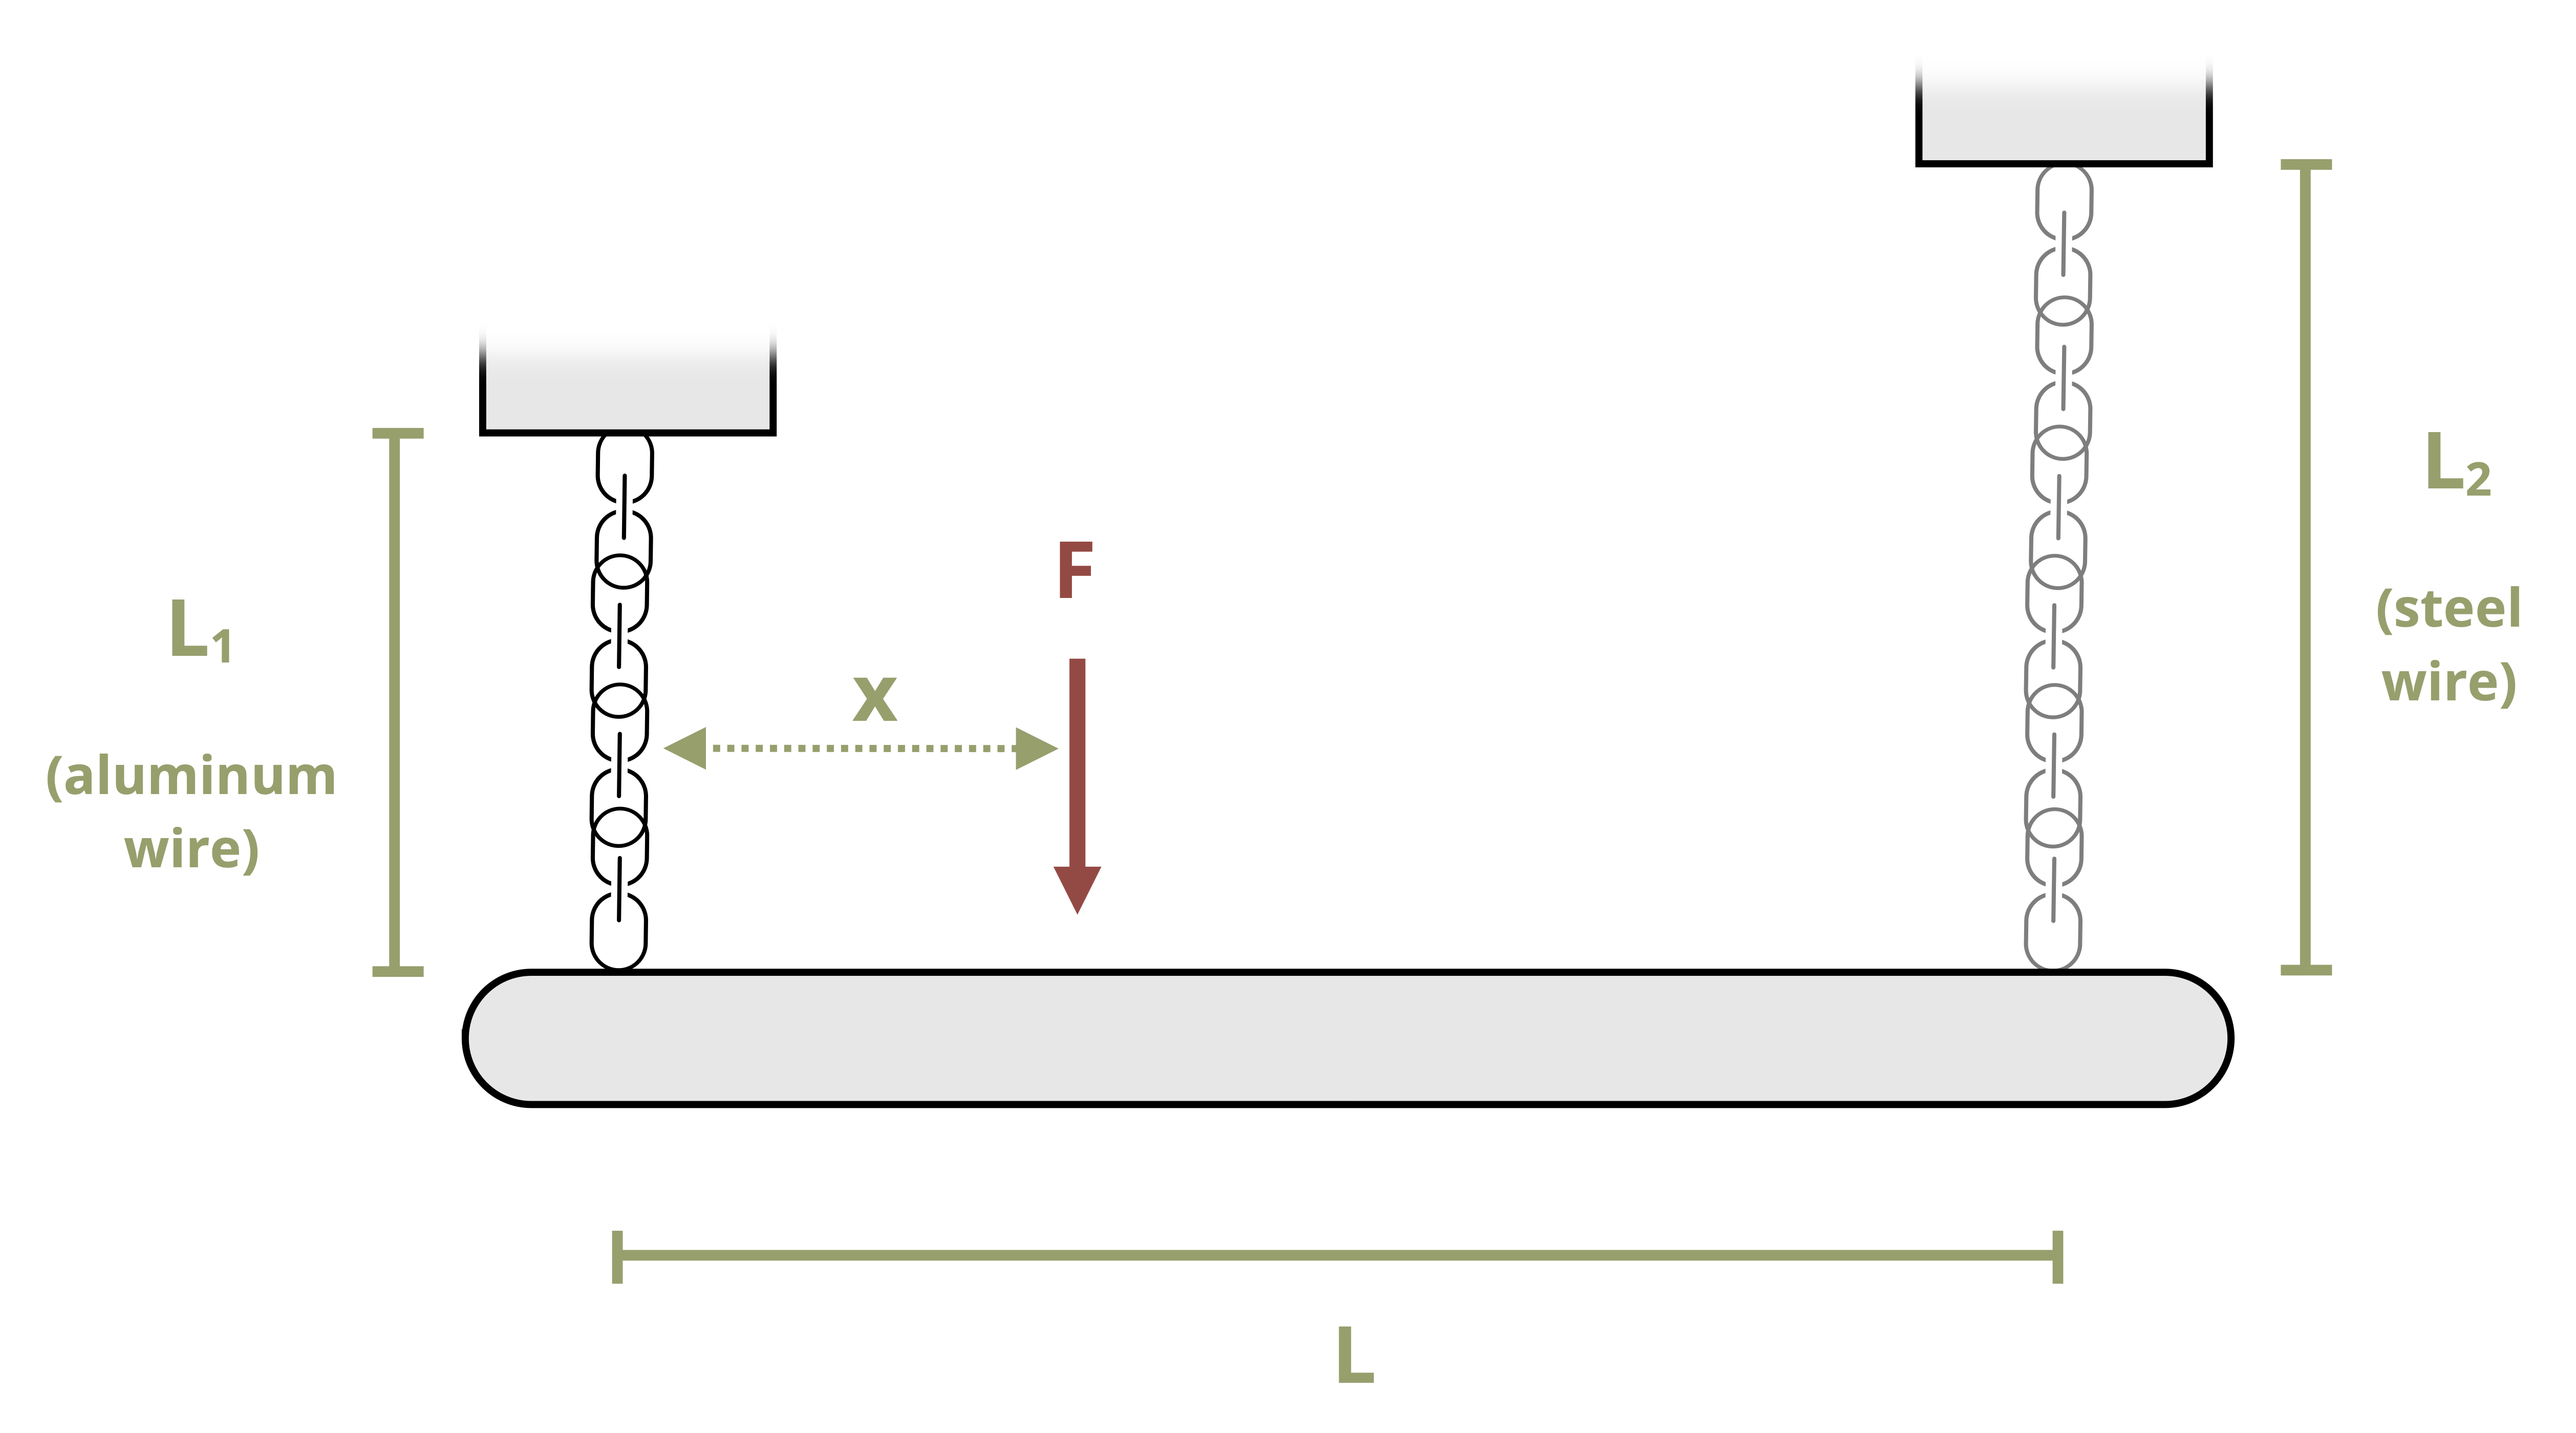
\includegraphics[keepaspectratio]{images/191.png}}
{[}Problem adapted from © Kurt Gramoll CC BY NC-SA 4.0{]}

\begin{Shaded}
\begin{Highlighting}[]
\NormalTok{\#| standalone: true}
\NormalTok{\#| viewerHeight: 600}
\NormalTok{\#| components: [viewer]}

\NormalTok{from shiny import App, render, ui, reactive}
\NormalTok{import random}
\NormalTok{import asyncio}
\NormalTok{import io}
\NormalTok{import math}
\NormalTok{import string}
\NormalTok{from datetime import datetime}
\NormalTok{from pathlib import Path}

\NormalTok{def generate\_random\_letters(length):}
\NormalTok{    \# Generate a random string of letters of specified length}
\NormalTok{    return \textquotesingle{}\textquotesingle{}.join(random.choice(string.ascii\_lowercase) for \_ in range(length))}

\NormalTok{problem\_ID="191"}
\NormalTok{L1=reactive.Value("\_\_")}
\NormalTok{L2=reactive.Value("\_\_")}
\NormalTok{F=reactive.Value("\_\_")}
\NormalTok{A=reactive.Value("\_\_")}
\NormalTok{L=reactive.Value("\_\_")}
\NormalTok{Esteel = 29000}
\NormalTok{Ealuminum = 10000}


\NormalTok{attempts=["Timestamp,Attempt,Answer,Feedback\textbackslash{}n"]}

\NormalTok{app\_ui = ui.page\_fluid(}
\NormalTok{    ui.markdown("**Please enter your ID number from your instructor and click to generate your problem**"),}
\NormalTok{    ui.input\_text("ID","", placeholder="Enter ID Number Here"),}
\NormalTok{    ui.input\_action\_button("generate\_problem", "Generate Problem", class\_="btn{-}primary"),}
\NormalTok{    ui.markdown("**Problem Statement**"),}
\NormalTok{    ui.output\_ui("ui\_problem\_statement"),}
\NormalTok{    ui.input\_text("answer","Your Answer in units of inches", placeholder="Please enter your answer"),}
\NormalTok{    ui.input\_action\_button("submit", "Submit Answer", class\_="btn{-}primary"),}
\NormalTok{    ui.download\_button("download", "Download File to Submit", class\_="btn{-}success"),}
\NormalTok{)}


\NormalTok{def server(input, output, session):}
\NormalTok{    \# Initialize a counter for attempts}
\NormalTok{    attempt\_counter = reactive.Value(0)}

\NormalTok{    @output}
\NormalTok{    @render.ui}
\NormalTok{    def ui\_problem\_statement():}
\NormalTok{        return[ui.markdown(f"A bar is attached to two wires, one steel and one aluminum. If the lengths of the wires L\textless{}sub\textgreater{}1\textless{}/sub\textgreater{} = \{L1()\} in. and L\textless{}sub\textgreater{}2\textless{}/sub\textgreater{} = \{L2()\} in., find the distance x that load F = \{F()\} kips must be placed at so that the bar remains horizontal after the load is applied. Both wires have the same cross{-}section area A = \{A()\} in.\textless{}sup\textgreater{}2\textless{}/sup\textgreater{}. Assume E\textless{}sub\textgreater{}steel\textless{}/sub\textgreater{} = 29,000 ksi, E\textless{}sub\textgreater{}aluminum\textless{}/sub\textgreater{} = 10,000 ksi and that the bar is of length L = \{L()\} in.")]}
    
\NormalTok{    @reactive.Effect}
\NormalTok{    @reactive.event(input.generate\_problem)}
\NormalTok{    def randomize\_vars():}
\NormalTok{        random.seed(input.ID())}
\NormalTok{        L1.set(random.randrange(50, 150, 1)/10)}
\NormalTok{        L2.set(round(L1()*2, 2))}
\NormalTok{        F.set(random.randrange(30, 150, 1)/10)}
\NormalTok{        A.set(random.randrange(2, 25, 1)/100)}
\NormalTok{        L.set(random.randrange(10, 20, 1))}
        
\NormalTok{    @reactive.Effect}
\NormalTok{    @reactive.event(input.submit)}
\NormalTok{    def \_():}
\NormalTok{        attempt\_counter.set(attempt\_counter() + 1)  \# Increment the attempt counter on each submission.}
\NormalTok{        PsPa = (L1()*Esteel*A())/(L2()*Ealuminum*A())}
\NormalTok{        Ps = (F()/(PsPa+1))*PsPa}
\NormalTok{        instr=(Ps*L())/F()}
\NormalTok{        if math.isclose(float(input.answer()), instr, rel\_tol=0.01):}
\NormalTok{            check = "*Correct*"}
\NormalTok{            correct\_indicator = "JL"}
\NormalTok{        else:}
\NormalTok{            check = "*Not Correct.*"}
\NormalTok{            correct\_indicator = "JG"}

\NormalTok{        \# Generate random parts for the encoded attempt.}
\NormalTok{        random\_start = generate\_random\_letters(4)}
\NormalTok{        random\_middle = generate\_random\_letters(4)}
\NormalTok{        random\_end = generate\_random\_letters(4)}
\NormalTok{        encoded\_attempt = f"\{random\_start\}\{problem\_ID\}{-}\{random\_middle\}\{attempt\_counter()\}\{correct\_indicator\}{-}\{random\_end\}\{input.ID()\}"}

\NormalTok{        \# Store the most recent encoded attempt in a reactive value so it persists across submissions}
\NormalTok{        session.encoded\_attempt = reactive.Value(encoded\_attempt)}

\NormalTok{        \# Append the attempt data to the attempts list without the encoded attempt}
\NormalTok{        attempts.append(f"\{datetime.now()\}, \{attempt\_counter()\}, \{input.answer()\}, \{check\}\textbackslash{}n")}

\NormalTok{        \# Show feedback to the user.}
\NormalTok{        feedback = ui.markdown(f"Your answer of \{input.answer()\} is \{check\}.")}
\NormalTok{        m = ui.modal(}
\NormalTok{            feedback,}
\NormalTok{            title="Feedback",}
\NormalTok{            easy\_close=True}
\NormalTok{        )}
\NormalTok{        ui.modal\_show(m)}

\NormalTok{    @session.download(filename=lambda: f"Problem\_Log{-}\{problem\_ID\}{-}\{input.ID()\}.csv")}
\NormalTok{    async def download():}
\NormalTok{        \# Start the CSV with the encoded attempt (without label)}
\NormalTok{        final\_encoded = session.encoded\_attempt() if session.encoded\_attempt is not None else "No attempts"}
\NormalTok{        yield f"\{final\_encoded\}\textbackslash{}n\textbackslash{}n"}
        
\NormalTok{        \# Write the header for the remaining CSV data once}
\NormalTok{        yield "Timestamp,Attempt,Answer,Feedback\textbackslash{}n"}
        
\NormalTok{        \# Write the attempts data, ensure that the header from the attempts list is not written again}
\NormalTok{        for attempt in attempts[1:]:  \# Skip the first element which is the header}
\NormalTok{            await asyncio.sleep(0.25)  \# This delay may not be necessary; adjust as needed}
\NormalTok{            yield attempt}


\NormalTok{\# App installation}
\NormalTok{app = App(app\_ui, server)}
\end{Highlighting}
\end{Shaded}

\chapter*{Problem 5.34 - Statically Indeterminate Axial
Loads}\label{problem-5.34---statically-indeterminate-axial-loads}
\addcontentsline{toc}{chapter}{Problem 5.34 - Statically Indeterminate
Axial Loads}

\markboth{Problem 5.34 - Statically Indeterminate Axial Loads}{Problem
5.34 - Statically Indeterminate Axial Loads}

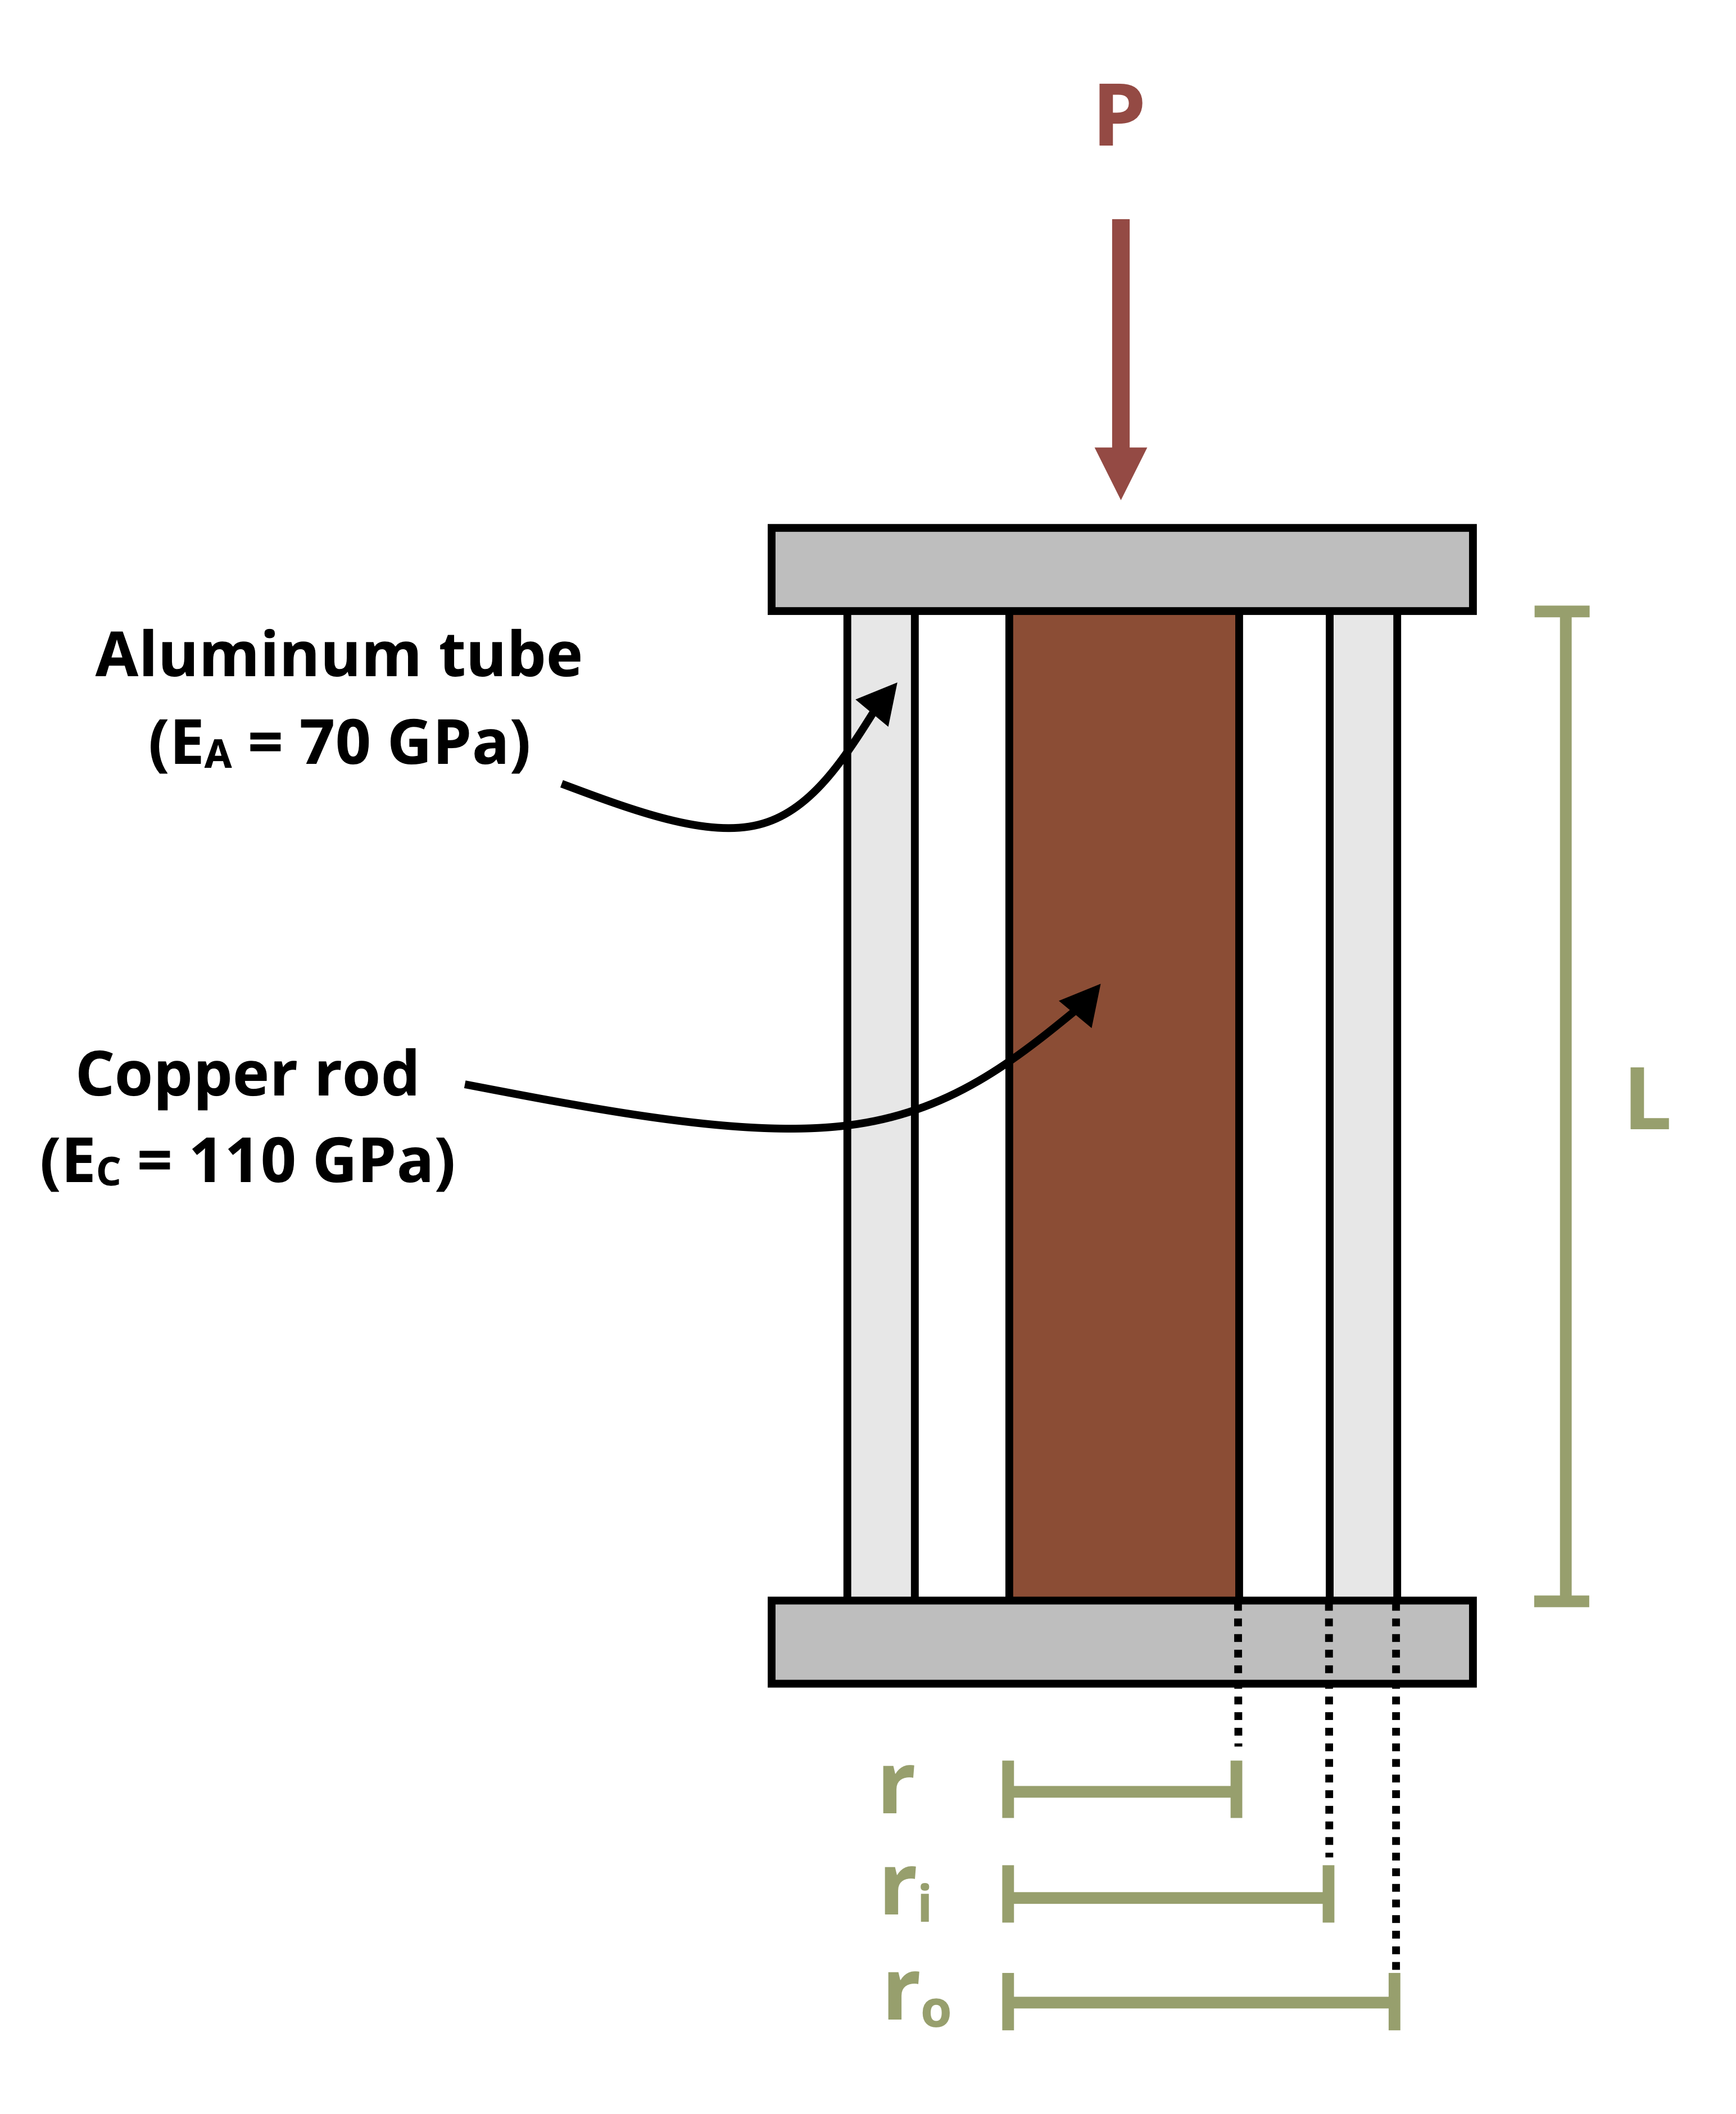
\includegraphics[width=3.64583in,height=\textheight,keepaspectratio]{images/192.png}
{[}Problem adapted from © Kurt Gramoll CC BY NC-SA 4.0{]}

\begin{Shaded}
\begin{Highlighting}[]
\NormalTok{\#| standalone: true}
\NormalTok{\#| viewerHeight: 600}
\NormalTok{\#| components: [viewer]}

\NormalTok{from shiny import App, render, ui, reactive}
\NormalTok{import random}
\NormalTok{import asyncio}
\NormalTok{import io}
\NormalTok{import math}
\NormalTok{import string}
\NormalTok{from datetime import datetime}
\NormalTok{from pathlib import Path}

\NormalTok{def generate\_random\_letters(length):}
\NormalTok{    \# Generate a random string of letters of specified length}
\NormalTok{    return \textquotesingle{}\textquotesingle{}.join(random.choice(string.ascii\_lowercase) for \_ in range(length)) }

\NormalTok{problem\_ID="192"}
\NormalTok{r=reactive.Value("\_\_")}
\NormalTok{ri=reactive.Value("\_\_")}
\NormalTok{ro=reactive.Value("\_\_")}
\NormalTok{L=reactive.Value("\_\_")}
\NormalTok{dL=reactive.Value("\_\_")}
\NormalTok{Ecopper = 110}
\NormalTok{Ealuminum = 70}

\NormalTok{attempts=["Timestamp,Attempt,Answer,Feedback\textbackslash{}n"]}

\NormalTok{app\_ui = ui.page\_fluid(}
\NormalTok{    ui.markdown("**Please enter your ID number from your instructor and click to generate your problem**"),}
\NormalTok{    ui.input\_text("ID","", placeholder="Enter ID Number Here"),}
\NormalTok{    ui.input\_action\_button("generate\_problem", "Generate Problem", class\_="btn{-}primary"),}
\NormalTok{    ui.markdown("**Problem Statement**"),}
\NormalTok{    ui.output\_ui("ui\_problem\_statement"),}
\NormalTok{    ui.input\_text("answer","Your Answer in units of kN", placeholder="Please enter your answer"),}
\NormalTok{    ui.input\_action\_button("submit", "Submit Answer", class\_="btn{-}primary"),}
\NormalTok{    ui.download\_button("download", "Download File to Submit", class\_="btn{-}success"),}
\NormalTok{)}

\NormalTok{def server(input, output, session):}
\NormalTok{    \# Initialize a counter for attempts}
\NormalTok{    attempt\_counter = reactive.Value(0)}

\NormalTok{    @output}
\NormalTok{    @render.ui}
\NormalTok{    def ui\_problem\_statement():}
\NormalTok{        return[ui.markdown(f"A copper circular rod of radius r = \{r()\} cm is inserted into an aluminum tube with inner radius r\textless{}sub\textgreater{}i\textless{}/sub\textgreater{} = \{ri()\} cm and outer radius r\textless{}sub\textgreater{}o\textless{}/sub\textgreater{} = \{ro()\} cm as shown. Load P is applied to the rigid top plate. If length L = \{L()\} cm, what load P will cause the plate to deflect dL = \{dL()\} mm downward? Assume E\textless{}sub\textgreater{}copper\textless{}/sub\textgreater{} = 110 GPa and E\textless{}sub\textgreater{}aluminum\textless{}/sub\textgreater{} = 70 GPa")]}
    
\NormalTok{    @reactive.Effect}
\NormalTok{    @reactive.event(input.generate\_problem)}
\NormalTok{    def randomize\_vars():}
\NormalTok{        random.seed(input.ID())}
\NormalTok{        r.set(random.randrange(20, 60, 1)/10)}
\NormalTok{        ri.set(round(r()*1.25, 2))}
\NormalTok{        ro.set(round(r()*1.5, 2))}
\NormalTok{        L.set(random.randrange(150, 300, 1)/10)}
\NormalTok{        dL.set(random.randrange(10, 50, 1)/100)}
        
\NormalTok{    @reactive.Effect}
\NormalTok{    @reactive.event(input.submit)}
\NormalTok{    def \_():}
\NormalTok{        attempt\_counter.set(attempt\_counter() + 1)  \# Increment the attempt counter on each submission.}
\NormalTok{        instr=(((dL()*Ecopper*r()**2*math.pi)/L()) + ((dL()*Ealuminum*(ro()**2{-}ri()**2)*math.pi)/L()))*10}
\NormalTok{        if math.isclose(float(input.answer()), instr, rel\_tol=0.01):}
\NormalTok{            check = "*Correct*"}
\NormalTok{            correct\_indicator = "JL"}
\NormalTok{        else:}
\NormalTok{            check = "*Not Correct.*"}
\NormalTok{            correct\_indicator = "JG"}

\NormalTok{        \# Generate random parts for the encoded attempt.}
\NormalTok{        random\_start = generate\_random\_letters(4)}
\NormalTok{        random\_middle = generate\_random\_letters(4)}
\NormalTok{        random\_end = generate\_random\_letters(4)}
\NormalTok{        encoded\_attempt = f"\{random\_start\}\{problem\_ID\}{-}\{random\_middle\}\{attempt\_counter()\}\{correct\_indicator\}{-}\{random\_end\}\{input.ID()\}"}

\NormalTok{        \# Store the most recent encoded attempt in a reactive value so it persists across submissions}
\NormalTok{        session.encoded\_attempt = reactive.Value(encoded\_attempt)}

\NormalTok{        \# Append the attempt data to the attempts list without the encoded attempt}
\NormalTok{        attempts.append(f"\{datetime.now()\}, \{attempt\_counter()\}, \{input.answer()\}, \{check\}\textbackslash{}n")}

\NormalTok{        \# Show feedback to the user.}
\NormalTok{        feedback = ui.markdown(f"Your answer of \{input.answer()\} is \{check\}.")}
\NormalTok{        m = ui.modal(}
\NormalTok{            feedback,}
\NormalTok{            title="Feedback",}
\NormalTok{            easy\_close=True}
\NormalTok{        )}
\NormalTok{        ui.modal\_show(m)}

\NormalTok{    @session.download(filename=lambda: f"Problem\_Log{-}\{problem\_ID\}{-}\{input.ID()\}.csv")}
\NormalTok{    async def download():}
\NormalTok{        \# Start the CSV with the encoded attempt (without label)}
\NormalTok{        final\_encoded = session.encoded\_attempt() if session.encoded\_attempt is not None else "No attempts"}
\NormalTok{        yield f"\{final\_encoded\}\textbackslash{}n\textbackslash{}n"}
        
\NormalTok{        \# Write the header for the remaining CSV data once}
\NormalTok{        yield "Timestamp,Attempt,Answer,Feedback\textbackslash{}n"}
        
\NormalTok{        \# Write the attempts data, ensure that the header from the attempts list is not written again}
\NormalTok{        for attempt in attempts[1:]:  \# Skip the first element which is the header}
\NormalTok{            await asyncio.sleep(0.25)  \# This delay may not be necessary; adjust as needed}
\NormalTok{            yield attempt}

\NormalTok{\# App installation}
\NormalTok{app = App(app\_ui, server)}
\end{Highlighting}
\end{Shaded}

\chapter*{Problem 5.35 - Statically Indeterminate Axial
Loads}\label{problem-5.35---statically-indeterminate-axial-loads}
\addcontentsline{toc}{chapter}{Problem 5.35 - Statically Indeterminate
Axial Loads}

\markboth{Problem 5.35 - Statically Indeterminate Axial Loads}{Problem
5.35 - Statically Indeterminate Axial Loads}

\pandocbounded{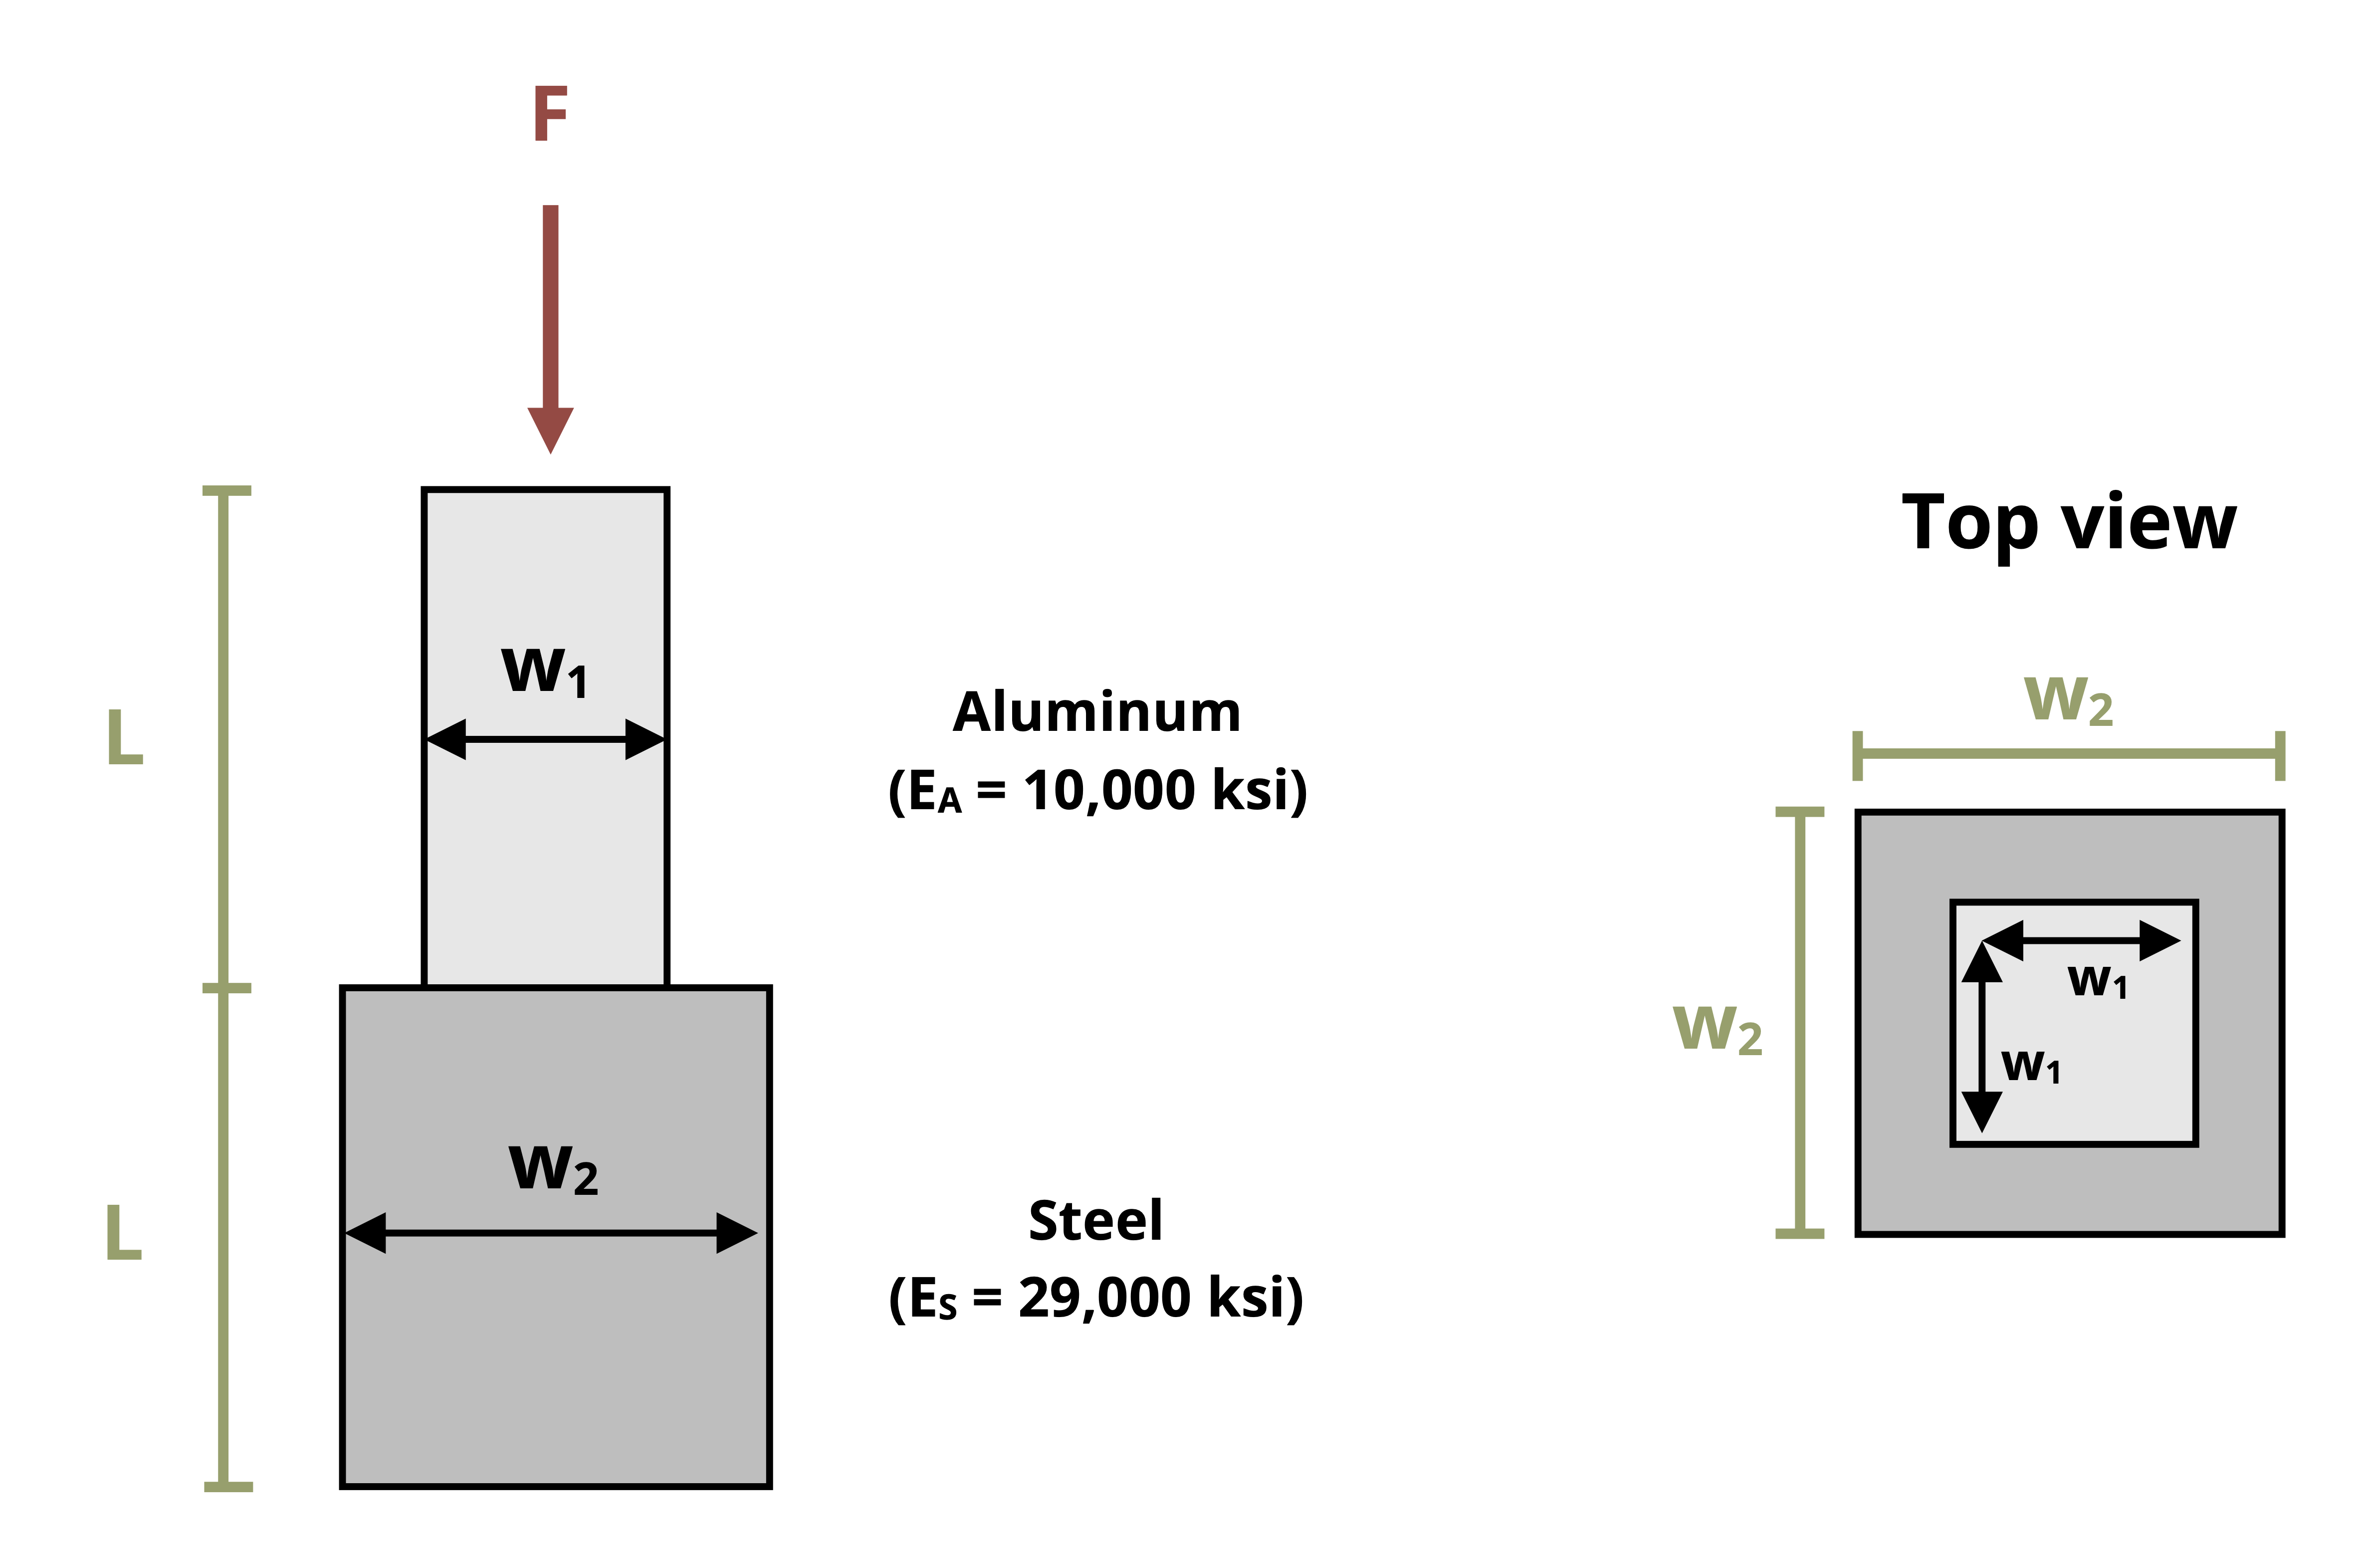
\includegraphics[keepaspectratio]{images/193.png}}
{[}Problem adapted from © Kurt Gramoll CC BY NC-SA 4.0{]}

\begin{Shaded}
\begin{Highlighting}[]
\NormalTok{\#| standalone: true}
\NormalTok{\#| viewerHeight: 600}
\NormalTok{\#| components: [viewer]}

\NormalTok{from shiny import App, render, ui, reactive}
\NormalTok{import random}
\NormalTok{import asyncio}
\NormalTok{import io}
\NormalTok{import math}
\NormalTok{import string}
\NormalTok{from datetime import datetime}
\NormalTok{from pathlib import Path}

\NormalTok{def generate\_random\_letters(length):}
\NormalTok{    \# Generate a random string of letters of specified length}
\NormalTok{    return \textquotesingle{}\textquotesingle{}.join(random.choice(string.ascii\_lowercase) for \_ in range(length)) }

\NormalTok{problem\_ID="193"}
\NormalTok{F=reactive.Value("\_\_")}
\NormalTok{w1=reactive.Value("\_\_")}
\NormalTok{w2=reactive.Value("\_\_")}
\NormalTok{L=reactive.Value("\_\_")}
\NormalTok{Esteel = 29000}
\NormalTok{Ealuminum = 10000}



\NormalTok{attempts=["Timestamp,Attempt,Answer,Feedback\textbackslash{}n"]}

\NormalTok{app\_ui = ui.page\_fluid(}
\NormalTok{    ui.markdown("**Please enter your ID number from your instructor and click to generate your problem**"),}
\NormalTok{    ui.input\_text("ID","", placeholder="Enter ID Number Here"),}
\NormalTok{    ui.input\_action\_button("generate\_problem", "Generate Problem", class\_="btn{-}primary"),}
\NormalTok{    ui.markdown("**Problem Statement**"),}
\NormalTok{    ui.output\_ui("ui\_problem\_statement"),}
\NormalTok{    ui.input\_text("answer","Your Answer in units of inches", placeholder="Please enter your answer"),}
\NormalTok{    ui.input\_action\_button("submit", "Submit Answer", class\_="btn{-}primary"),}
\NormalTok{    ui.download\_button("download", "Download File to Submit", class\_="btn{-}success"),}
\NormalTok{)}


\NormalTok{def server(input, output, session):}
\NormalTok{    \# Initialize a counter for attempts}
\NormalTok{    attempt\_counter = reactive.Value(0)}

\NormalTok{    @output}
\NormalTok{    @render.ui}
\NormalTok{    def ui\_problem\_statement():}
\NormalTok{        return[ui.markdown(f"Two blocks with square cross{-}sections are stacked as shown, with the top block inserted into the bottom block and subjected to load F = \{F()\} kips. The top block is aluminum (E = 10,000 ksi) with side length w\textless{}sub\textgreater{}1\textless{}/sub\textgreater{} = \{w1()\} in.  and the bottom block is steel (E = 29,000 ksi) with side length w\textless{}sub\textgreater{}2\textless{}/sub\textgreater{} = \{w2()\} in. If length L = \{L()\} in., what is the total deflection of the top surface? Ignore the weight of the blocks. ")]}
    
\NormalTok{    @reactive.Effect}
\NormalTok{    @reactive.event(input.generate\_problem)}
\NormalTok{    def randomize\_vars():}
\NormalTok{        random.seed(input.ID())}
\NormalTok{        F.set(random.randrange(20, 100, 1)/10)}
\NormalTok{        w1.set(random.randrange(15, 50, 1)/10)}
\NormalTok{        w2.set(round(w1()*1.5))}
\NormalTok{        L.set(random.randrange(50, 200, 1)/10)}
        
\NormalTok{    @reactive.Effect}
\NormalTok{    @reactive.event(input.submit)}
\NormalTok{    def \_():}
\NormalTok{        attempt\_counter.set(attempt\_counter() + 1)  \# Increment the attempt counter on each submission.}
\NormalTok{        instr=F()*L()*((1/((w1()**2)*Ealuminum)) + (1/((w2()**2)*Esteel)))}
\NormalTok{        if math.isclose(float(input.answer()), instr, rel\_tol=0.01):}
\NormalTok{            check = "*Correct*"}
\NormalTok{            correct\_indicator = "JL"}
\NormalTok{        else:}
\NormalTok{            check = "*Not Correct.*"}
\NormalTok{            correct\_indicator = "JG"}

\NormalTok{        \# Generate random parts for the encoded attempt.}
\NormalTok{        random\_start = generate\_random\_letters(4)}
\NormalTok{        random\_middle = generate\_random\_letters(4)}
\NormalTok{        random\_end = generate\_random\_letters(4)}
\NormalTok{        encoded\_attempt = f"\{random\_start\}\{problem\_ID\}{-}\{random\_middle\}\{attempt\_counter()\}\{correct\_indicator\}{-}\{random\_end\}\{input.ID()\}"}

\NormalTok{        \# Store the most recent encoded attempt in a reactive value so it persists across submissions}
\NormalTok{        session.encoded\_attempt = reactive.Value(encoded\_attempt)}

\NormalTok{        \# Append the attempt data to the attempts list without the encoded attempt}
\NormalTok{        attempts.append(f"\{datetime.now()\}, \{attempt\_counter()\}, \{input.answer()\}, \{check\}\textbackslash{}n")}

\NormalTok{        \# Show feedback to the user.}
\NormalTok{        feedback = ui.markdown(f"Your answer of \{input.answer()\} is \{check\}.")}
\NormalTok{        m = ui.modal(}
\NormalTok{            feedback,}
\NormalTok{            title="Feedback",}
\NormalTok{            easy\_close=True}
\NormalTok{        )}
\NormalTok{        ui.modal\_show(m)}

\NormalTok{    @session.download(filename=lambda: f"Problem\_Log{-}\{problem\_ID\}{-}\{input.ID()\}.csv")}
\NormalTok{    async def download():}
\NormalTok{        \# Start the CSV with the encoded attempt (without label)}
\NormalTok{        final\_encoded = session.encoded\_attempt() if session.encoded\_attempt is not None else "No attempts"}
\NormalTok{        yield f"\{final\_encoded\}\textbackslash{}n\textbackslash{}n"}
        
\NormalTok{        \# Write the header for the remaining CSV data once}
\NormalTok{        yield "Timestamp,Attempt,Answer,Feedback\textbackslash{}n"}
        
\NormalTok{        \# Write the attempts data, ensure that the header from the attempts list is not written again}
\NormalTok{        for attempt in attempts[1:]:  \# Skip the first element which is the header}
\NormalTok{            await asyncio.sleep(0.25)  \# This delay may not be necessary; adjust as needed}
\NormalTok{            yield attempt}


\NormalTok{\# App installation}
\NormalTok{app = App(app\_ui, server)}
\end{Highlighting}
\end{Shaded}

\chapter*{Problem 5.36 - Statically Indeterminate Axial
Loads}\label{problem-5.36---statically-indeterminate-axial-loads}
\addcontentsline{toc}{chapter}{Problem 5.36 - Statically Indeterminate
Axial Loads}

\markboth{Problem 5.36 - Statically Indeterminate Axial Loads}{Problem
5.36 - Statically Indeterminate Axial Loads}

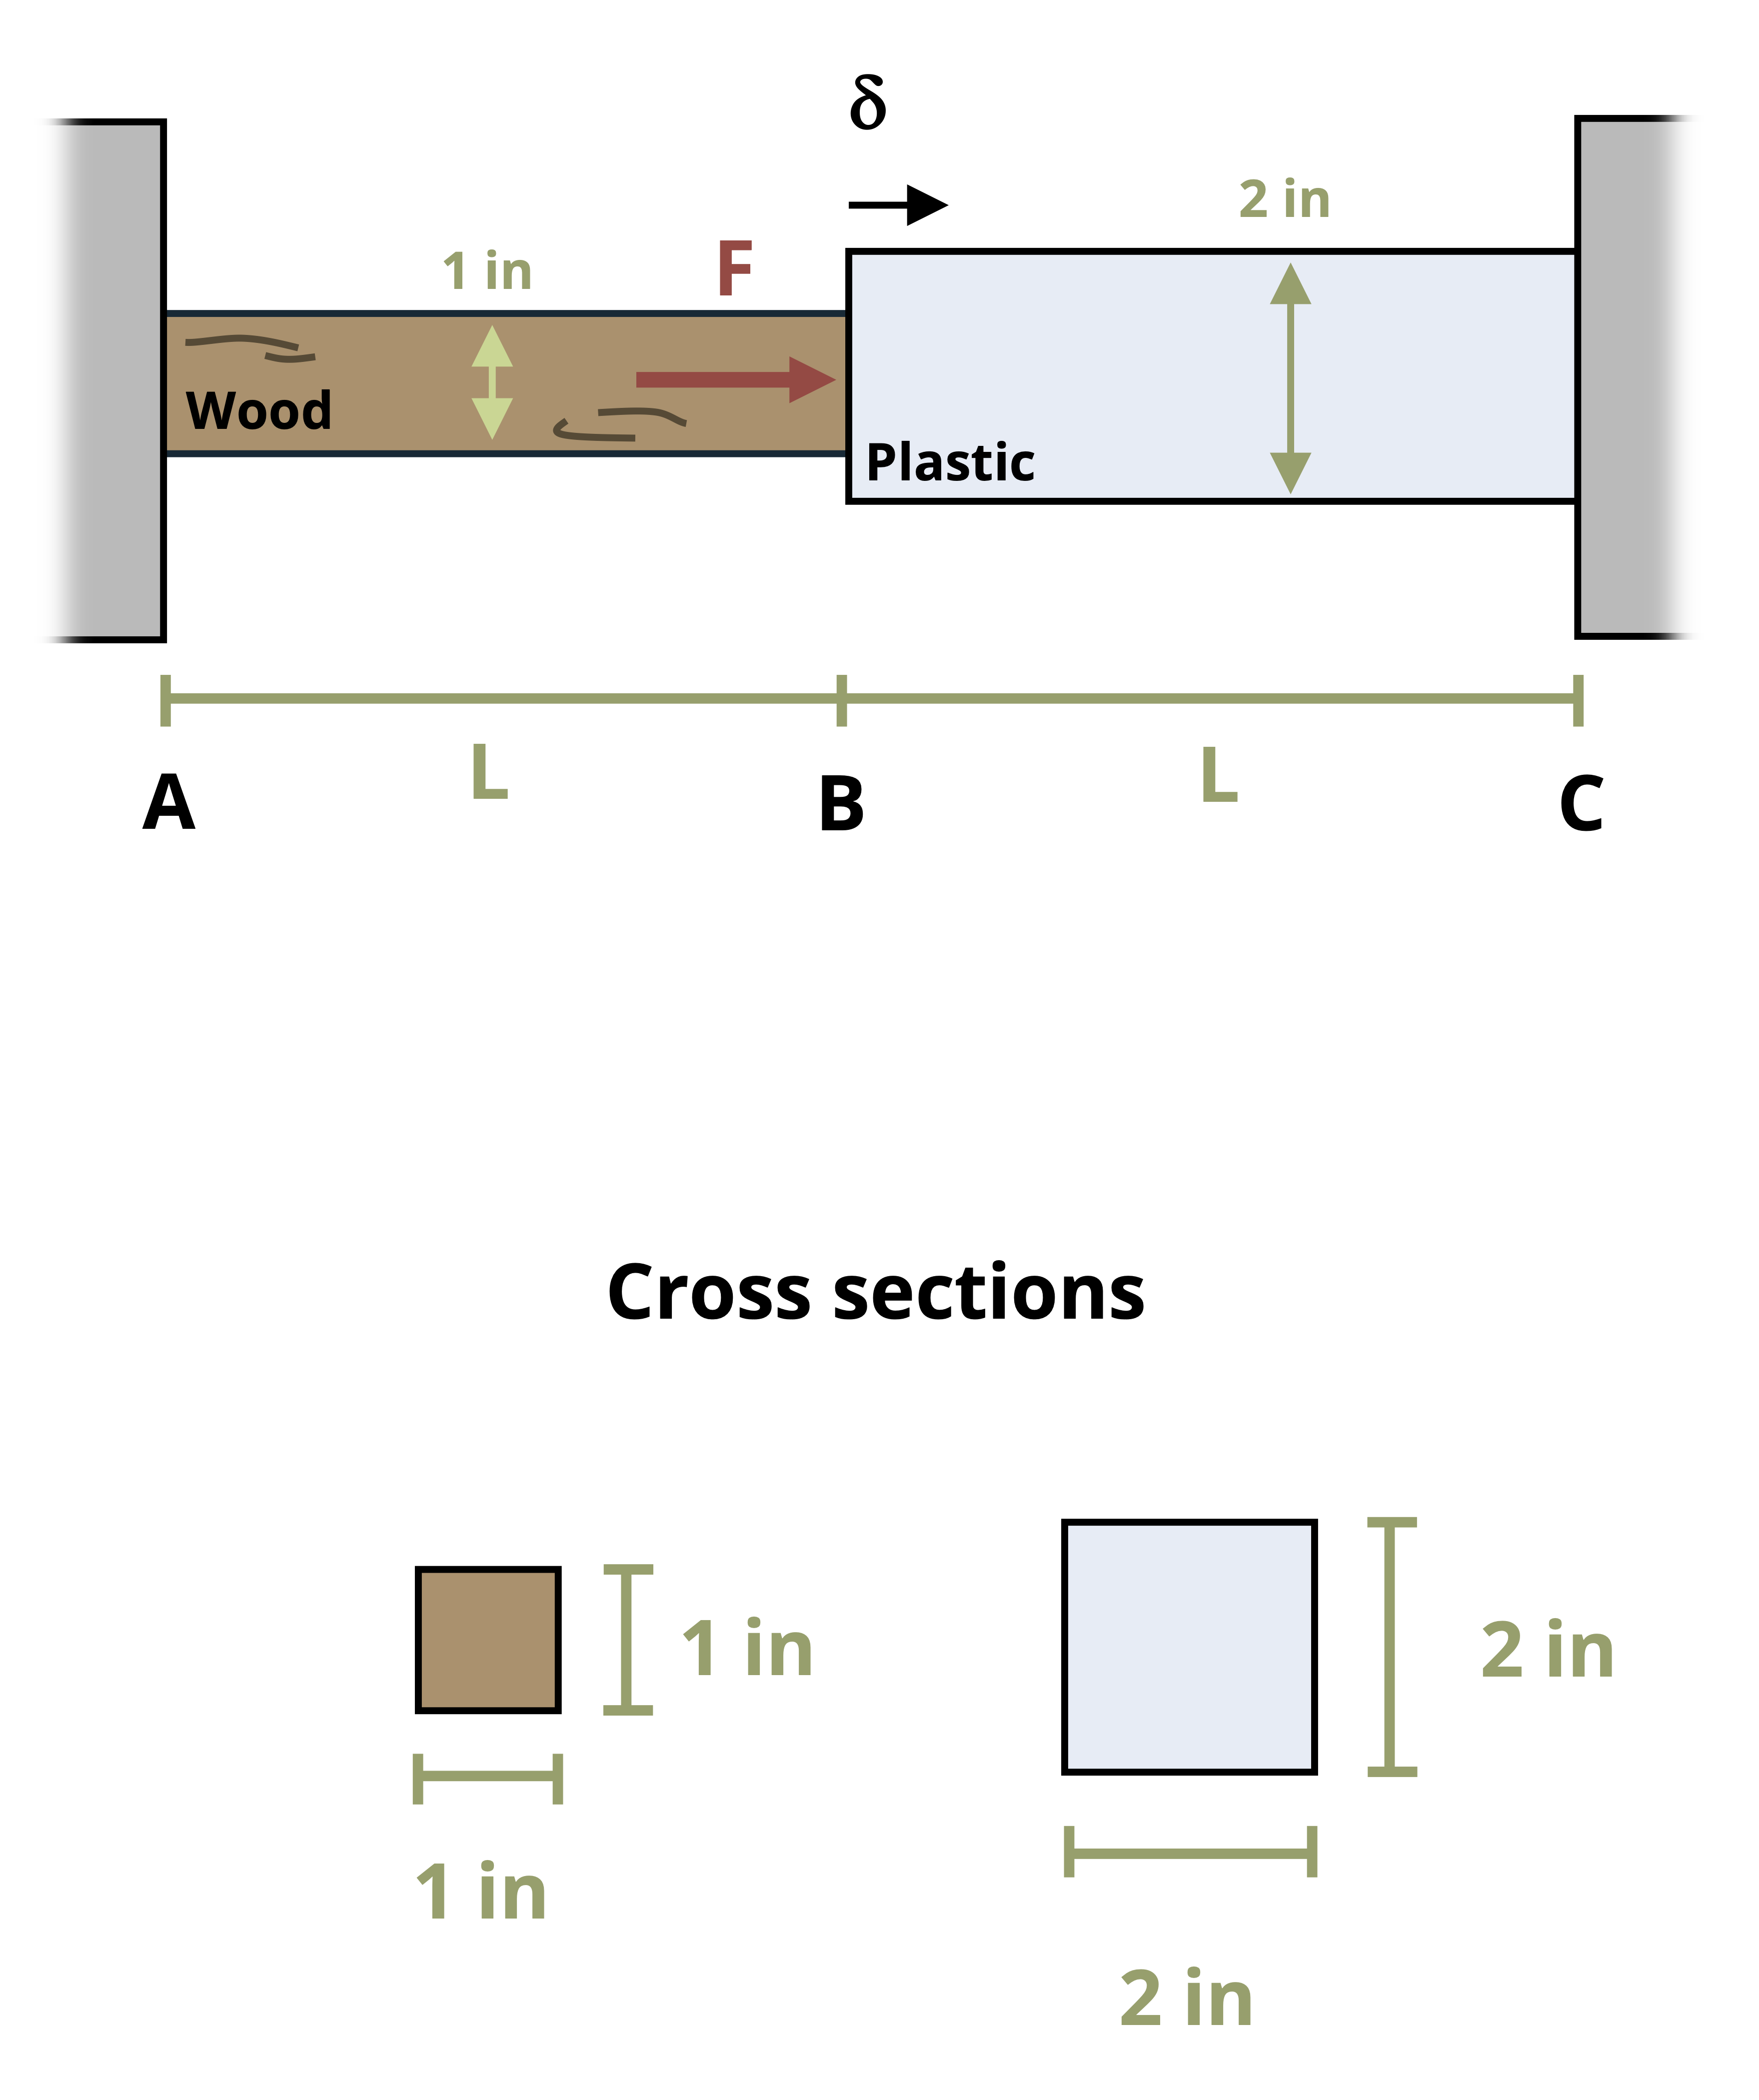
\includegraphics[width=3.64583in,height=\textheight,keepaspectratio]{images/246.png}
{[}Problem adapted from © Kurt Gramoll CC BY NC-SA 4.0{]}

\begin{Shaded}
\begin{Highlighting}[]
\NormalTok{\#| standalone: true}
\NormalTok{\#| viewerHeight: 600}
\NormalTok{\#| components: [viewer]}

\NormalTok{from shiny import App, render, ui, reactive}
\NormalTok{import random}
\NormalTok{import asyncio}
\NormalTok{import io}
\NormalTok{import math}
\NormalTok{import string}
\NormalTok{from datetime import datetime}
\NormalTok{from pathlib import Path}

\NormalTok{def generate\_random\_letters(length):}
\NormalTok{    \# Generate a random string of letters of specified length}
\NormalTok{    return \textquotesingle{}\textquotesingle{}.join(random.choice(string.ascii\_lowercase) for \_ in range(length)) }

\NormalTok{problem\_ID="246"}
\NormalTok{d=reactive.Value("\_\_")}
\NormalTok{L=reactive.Value("\_\_")}
\NormalTok{Eplastic=reactive.Value("\_\_")}
\NormalTok{Ewood=1750}

\NormalTok{attempts=["Timestamp,Attempt,Answer,Feedback\textbackslash{}n"]}

\NormalTok{app\_ui = ui.page\_fluid(}
\NormalTok{    ui.markdown("**Please enter your ID number from your instructor and click to generate your problem**"),}
\NormalTok{    ui.input\_text("ID","", placeholder="Enter ID Number Here"),}
\NormalTok{    ui.input\_action\_button("generate\_problem", "Generate Problem", class\_="btn{-}primary"),}
\NormalTok{    ui.markdown("**Problem Statement**"),}
\NormalTok{    ui.output\_ui("ui\_problem\_statement"),}
\NormalTok{    ui.input\_text("answer","Your Answer in units of lb", placeholder="Please enter your answer"),}
\NormalTok{    ui.input\_action\_button("submit", "Submit Answer", class\_="btn{-}primary"),}
\NormalTok{    ui.download\_button("download", "Download File to Submit", class\_="btn{-}success"),}
\NormalTok{)}


\NormalTok{def server(input, output, session):}
\NormalTok{    \# Initialize a counter for attempts}
\NormalTok{    attempt\_counter = reactive.Value(0)}

\NormalTok{    @output}
\NormalTok{    @render.ui}
\NormalTok{    def ui\_problem\_statement():}
\NormalTok{        return[ui.markdown(f"Two square members are attached to two fixed walls as shown. Force F is applied at point B and point B is displaced d =  \{d()\} in. to the right. If L = \{L()\} in., E\textless{}sub\textgreater{}wood\textless{}/sub\textgreater{} = 1,750 ksi, and E\textless{}sub\textgreater{}plastic\textless{}/sub\textgreater{} = \{Eplastic()\} ksi, determine the applied force F. ")]}
    
\NormalTok{    @reactive.Effect}
\NormalTok{    @reactive.event(input.generate\_problem)}
\NormalTok{    def randomize\_vars():}
\NormalTok{        random.seed(input.ID())}
\NormalTok{        d.set(random.randrange(2, 8, 1)/1000)}
\NormalTok{        L.set(random.randrange(4, 15, 1))}
\NormalTok{        Eplastic.set(random.randrange(350, 900, 10))}
       
\NormalTok{    @reactive.Effect}
\NormalTok{    @reactive.event(input.submit)}
\NormalTok{    def \_():}
\NormalTok{        attempt\_counter.set(attempt\_counter() + 1)  \# Increment the attempt counter on each submission.}
\NormalTok{        instr= (d()*1*Ewood*1000)/L() {-} ({-}d()*4*Eplastic()*1000)/L() }
\NormalTok{        if math.isclose(float(input.answer()), instr, rel\_tol=0.01):}
\NormalTok{            check = "*Correct*"}
\NormalTok{            correct\_indicator = "JL"}
\NormalTok{        else:}
\NormalTok{            check = "*Not Correct.*"}
\NormalTok{            correct\_indicator = "JG"}

\NormalTok{        \# Generate random parts for the encoded attempt.}
\NormalTok{        random\_start = generate\_random\_letters(4)}
\NormalTok{        random\_middle = generate\_random\_letters(4)}
\NormalTok{        random\_end = generate\_random\_letters(4)}
\NormalTok{        encoded\_attempt = f"\{random\_start\}\{problem\_ID\}{-}\{random\_middle\}\{attempt\_counter()\}\{correct\_indicator\}{-}\{random\_end\}\{input.ID()\}"}

\NormalTok{        \# Store the most recent encoded attempt in a reactive value so it persists across submissions}
\NormalTok{        session.encoded\_attempt = reactive.Value(encoded\_attempt)}

\NormalTok{        \# Append the attempt data to the attempts list without the encoded attempt}
\NormalTok{        attempts.append(f"\{datetime.now()\}, \{attempt\_counter()\}, \{input.answer()\}, \{check\}\textbackslash{}n")}

\NormalTok{        \# Show feedback to the user.}
\NormalTok{        feedback = ui.markdown(f"Your answer of \{input.answer()\} is \{check\}.")}
\NormalTok{        m = ui.modal(}
\NormalTok{            feedback,}
\NormalTok{            title="Feedback",}
\NormalTok{            easy\_close=True}
\NormalTok{        )}
\NormalTok{        ui.modal\_show(m)}

\NormalTok{    @session.download(filename=lambda: f"Problem\_Log{-}\{problem\_ID\}{-}\{input.ID()\}.csv")}
\NormalTok{    async def download():}
\NormalTok{        \# Start the CSV with the encoded attempt (without label)}
\NormalTok{        final\_encoded = session.encoded\_attempt() if session.encoded\_attempt is not None else "No attempts"}
\NormalTok{        yield f"\{final\_encoded\}\textbackslash{}n\textbackslash{}n"}
        
\NormalTok{        \# Write the header for the remaining CSV data once}
\NormalTok{        yield "Timestamp,Attempt,Answer,Feedback\textbackslash{}n"}
        
\NormalTok{        \# Write the attempts data, ensure that the header from the attempts list is not written again}
\NormalTok{        for attempt in attempts[1:]:  \# Skip the first element which is the header}
\NormalTok{            await asyncio.sleep(0.25)  \# This delay may not be necessary; adjust as needed}
\NormalTok{            yield attempt}

\NormalTok{\# App installation}
\NormalTok{app = App(app\_ui, server)}
\end{Highlighting}
\end{Shaded}

\chapter*{Problem 5.37 - Statically Indeterminate Axial
Loads}\label{problem-5.37---statically-indeterminate-axial-loads}
\addcontentsline{toc}{chapter}{Problem 5.37 - Statically Indeterminate
Axial Loads}

\markboth{Problem 5.37 - Statically Indeterminate Axial Loads}{Problem
5.37 - Statically Indeterminate Axial Loads}

\pandocbounded{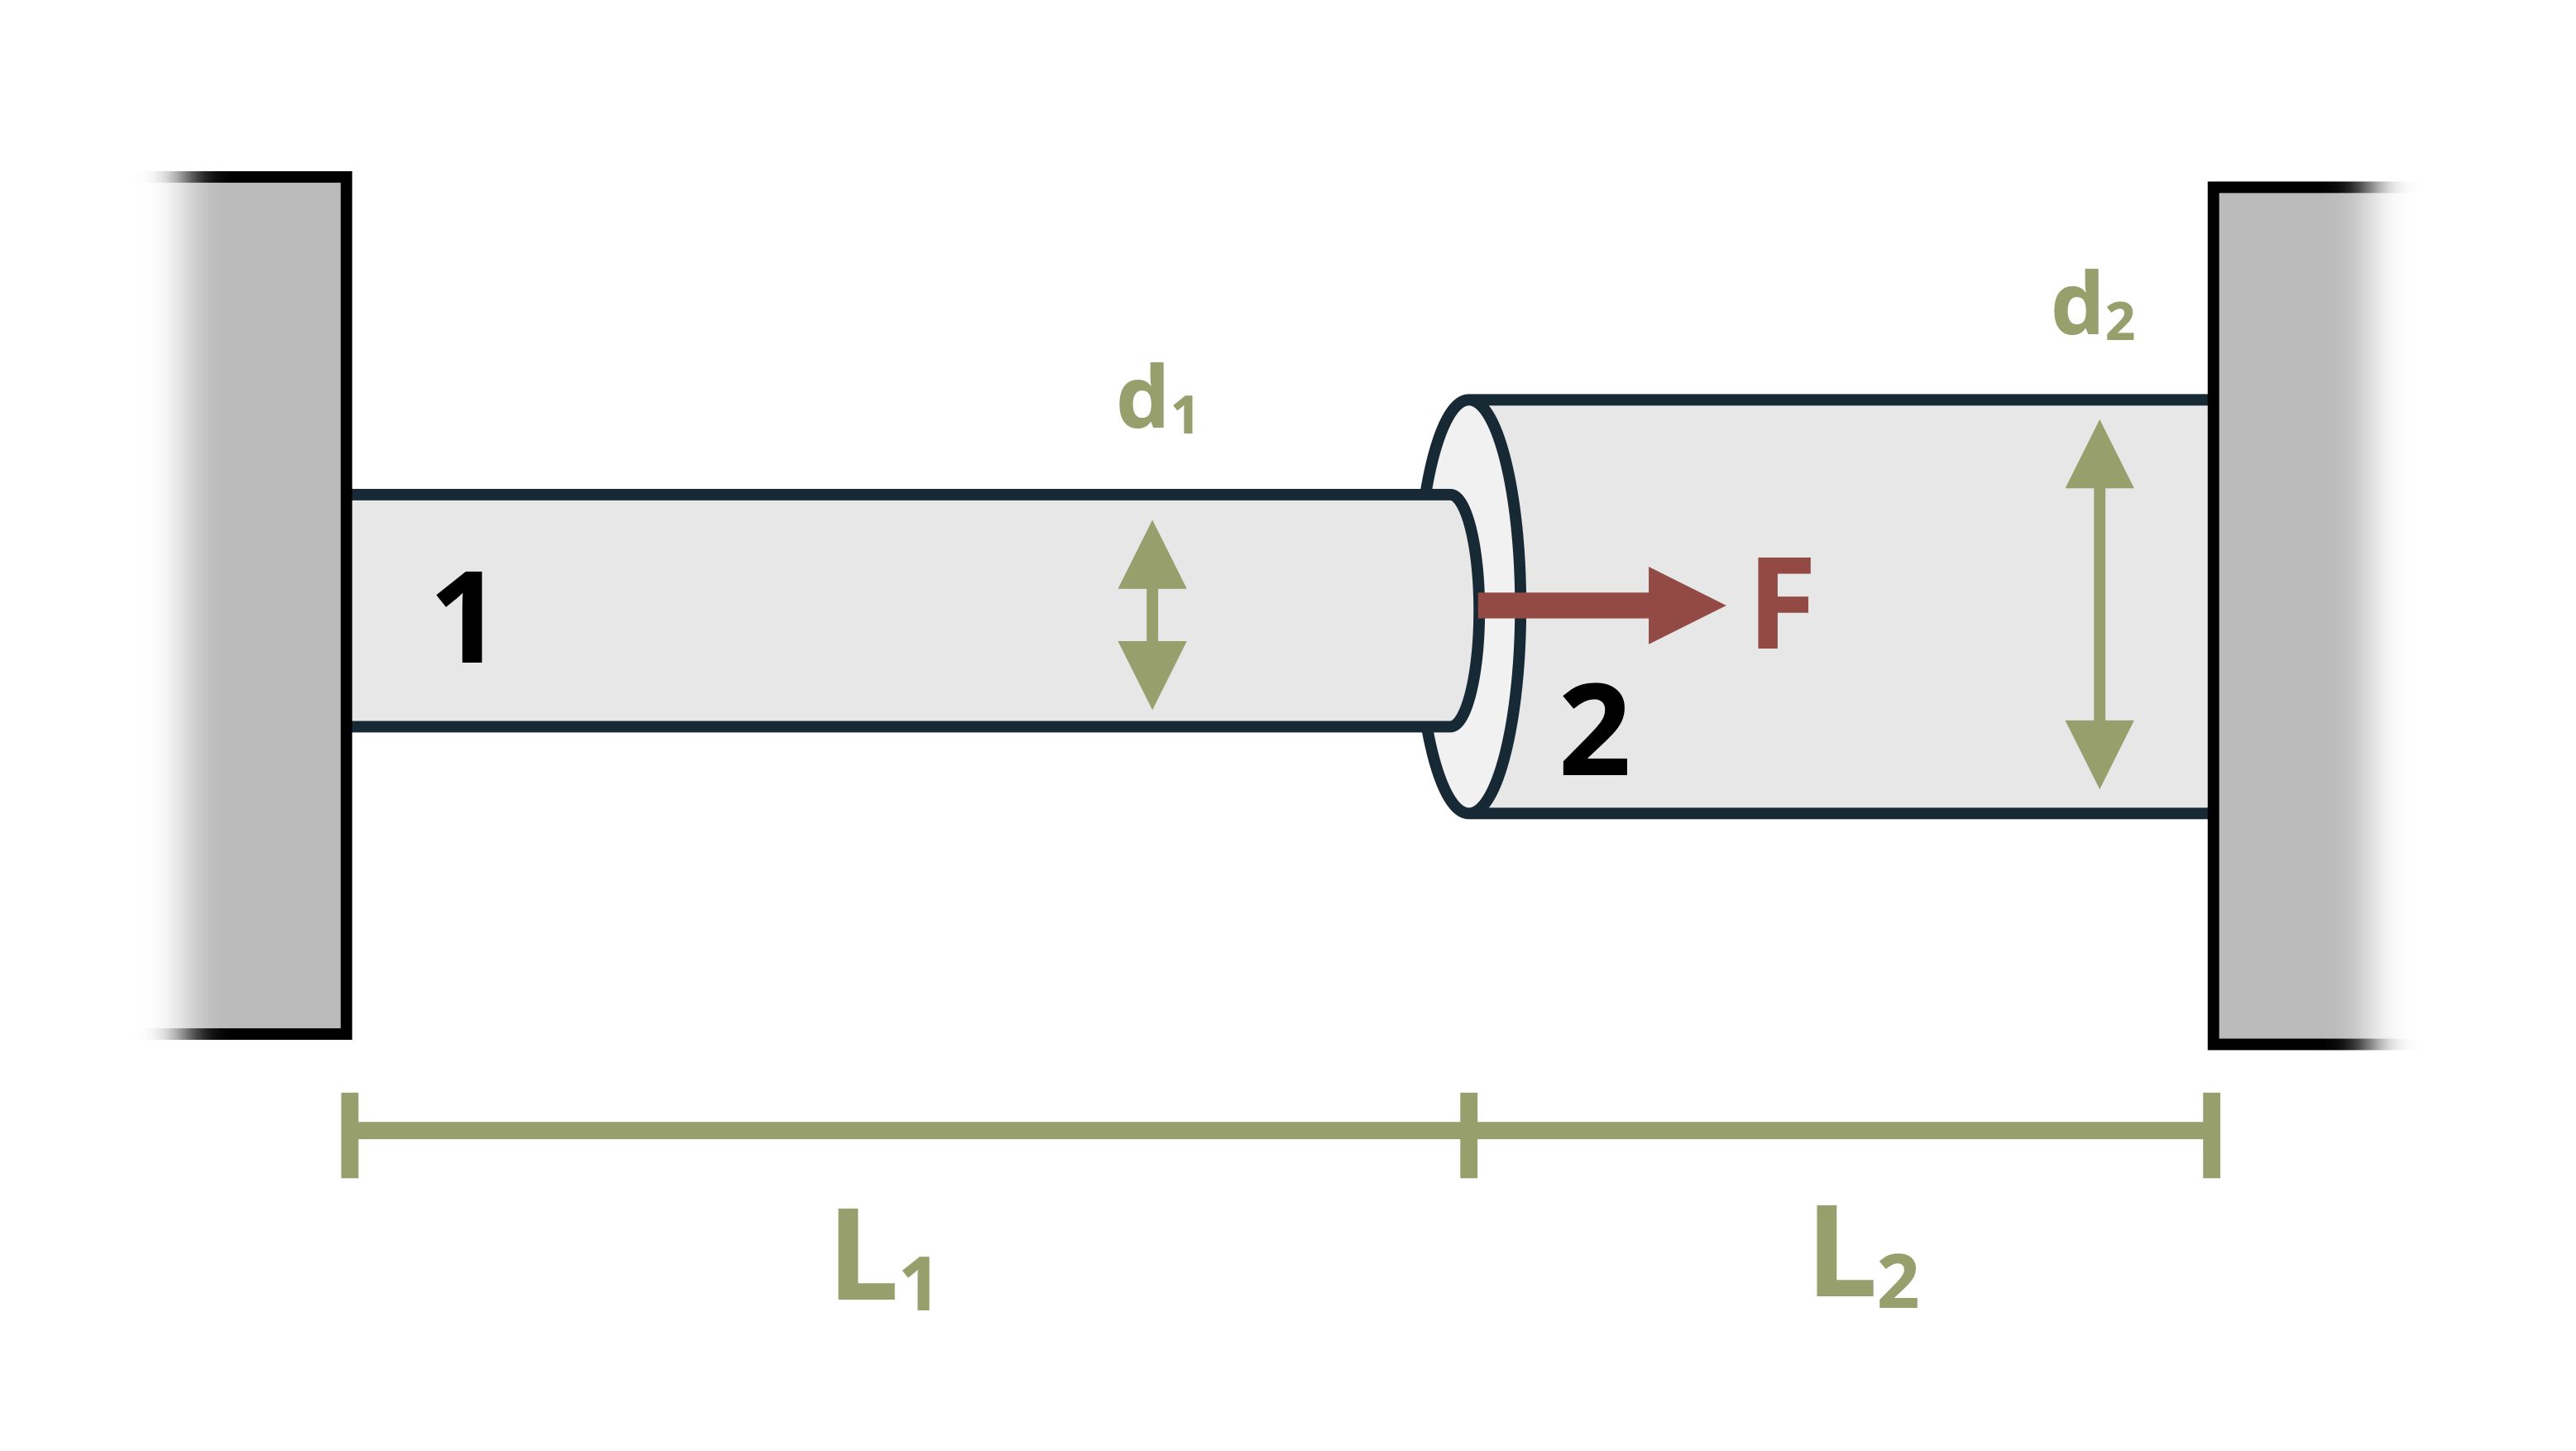
\includegraphics[keepaspectratio]{images/247.png}}
{[}Problem adapted from © Kurt Gramoll CC BY NC-SA 4.0{]}

\begin{Shaded}
\begin{Highlighting}[]
\NormalTok{\#| standalone: true}
\NormalTok{\#| viewerHeight: 600}
\NormalTok{\#| components: [viewer]}

\NormalTok{from shiny import App, render, ui, reactive}
\NormalTok{import random}
\NormalTok{import asyncio}
\NormalTok{import io}
\NormalTok{import math}
\NormalTok{import string}
\NormalTok{from datetime import datetime}
\NormalTok{from pathlib import Path}

\NormalTok{def generate\_random\_letters(length):}
\NormalTok{    \# Generate a random string of letters of specified length}
\NormalTok{    return \textquotesingle{}\textquotesingle{}.join(random.choice(string.ascii\_lowercase) for \_ in range(length)) }

\NormalTok{problem\_ID="247"}
\NormalTok{F=reactive.Value("\_\_")}
\NormalTok{d1=reactive.Value("\_\_")}
\NormalTok{d2=reactive.Value("\_\_")}
\NormalTok{L1=reactive.Value("\_\_")}
\NormalTok{L2=reactive.Value("\_\_")}
\NormalTok{Ewood=70}

\NormalTok{attempts=["Timestamp,Attempt,Answer,Feedback\textbackslash{}n"]}

\NormalTok{app\_ui = ui.page\_fluid(}
\NormalTok{    ui.markdown("**Please enter your ID number from your instructor and click to generate your problem**"),}
\NormalTok{    ui.input\_text("ID","", placeholder="Enter ID Number Here"),}
\NormalTok{    ui.input\_action\_button("generate\_problem", "Generate Problem", class\_="btn{-}primary"),}
\NormalTok{    ui.markdown("**Problem Statement**"),}
\NormalTok{    ui.output\_ui("ui\_problem\_statement"),}
\NormalTok{    ui.input\_text("answer","Your Answer in units of MPa", placeholder="Please enter your answer"),}
\NormalTok{    ui.input\_action\_button("submit", "Submit Answer", class\_="btn{-}primary"),}
\NormalTok{    ui.download\_button("download", "Download File to Submit", class\_="btn{-}success"),}
\NormalTok{)}


\NormalTok{def server(input, output, session):}
\NormalTok{    \# Initialize a counter for attempts}
\NormalTok{    attempt\_counter = reactive.Value(0)}

\NormalTok{    @output}
\NormalTok{    @render.ui}
\NormalTok{    def ui\_problem\_statement():}
\NormalTok{        return[ui.markdown(f"Two aluminum circular rods are attached to two fixed walls as shown. Assume E = 70 MPa for both cylinders, F = \{F()\} kN, d\textless{}sub\textgreater{}1\textless{}/sub\textgreater{} = \{d1()\} mm, d\textless{}sub\textgreater{}2\textless{}/sub\textgreater{}  = \{d2()\} mm, L\textless{}sub\textgreater{}1\textless{}/sub\textgreater{}  = \{L1()\} mm, and L\textless{}sub\textgreater{}2\textless{}/sub\textgreater{}  = \{L2()\} mm. Determine the normal stress in member 1.")]}
    
\NormalTok{    @reactive.Effect}
\NormalTok{    @reactive.event(input.generate\_problem)}
\NormalTok{    def randomize\_vars():}
\NormalTok{        random.seed(input.ID())}
\NormalTok{        F.set(random.randrange(20, 100, 1))}
\NormalTok{        d1.set(random.randrange(15, 50, 1))}
\NormalTok{        d2.set(round(d1()*1.5))}
\NormalTok{        L1.set(random.randrange(200, 800, 10))}
\NormalTok{        L2.set(round(L1()*(2/3)))}
       
        
\NormalTok{    @reactive.Effect}
\NormalTok{    @reactive.event(input.submit)}
\NormalTok{    def \_():}
\NormalTok{        attempt\_counter.set(attempt\_counter() + 1)  \# Increment the attempt counter on each submission.}
\NormalTok{        LHS = (L1()/1000)/(math.pi*(d1()/2000)**2) + (L2()/1000)/(math.pi*(d2()/2000)**2)}
\NormalTok{        RHS = (F()*L2())/(math.pi*(d2()/2)**2)}
\NormalTok{        instr= (RHS/LHS)/(math.pi*(d1()/2000)**2)}
\NormalTok{        if math.isclose(float(input.answer()), instr, rel\_tol=0.01):}
\NormalTok{            check = "*Correct*"}
\NormalTok{            correct\_indicator = "JL"}
\NormalTok{        else:}
\NormalTok{            check = "*Not Correct.*"}
\NormalTok{            correct\_indicator = "JG"}

\NormalTok{        \# Generate random parts for the encoded attempt.}
\NormalTok{        random\_start = generate\_random\_letters(4)}
\NormalTok{        random\_middle = generate\_random\_letters(4)}
\NormalTok{        random\_end = generate\_random\_letters(4)}
\NormalTok{        encoded\_attempt = f"\{random\_start\}\{problem\_ID\}{-}\{random\_middle\}\{attempt\_counter()\}\{correct\_indicator\}{-}\{random\_end\}\{input.ID()\}"}

\NormalTok{        \# Store the most recent encoded attempt in a reactive value so it persists across submissions}
\NormalTok{        session.encoded\_attempt = reactive.Value(encoded\_attempt)}

\NormalTok{        \# Append the attempt data to the attempts list without the encoded attempt}
\NormalTok{        attempts.append(f"\{datetime.now()\}, \{attempt\_counter()\}, \{input.answer()\}, \{check\}\textbackslash{}n")}

\NormalTok{        \# Show feedback to the user.}
\NormalTok{        feedback = ui.markdown(f"Your answer of \{input.answer()\} is \{check\}.")}
\NormalTok{        m = ui.modal(}
\NormalTok{            feedback,}
\NormalTok{            title="Feedback",}
\NormalTok{            easy\_close=True}
\NormalTok{        )}
\NormalTok{        ui.modal\_show(m)}

\NormalTok{    @session.download(filename=lambda: f"Problem\_Log{-}\{problem\_ID\}{-}\{input.ID()\}.csv")}
\NormalTok{    async def download():}
\NormalTok{        \# Start the CSV with the encoded attempt (without label)}
\NormalTok{        final\_encoded = session.encoded\_attempt() if session.encoded\_attempt is not None else "No attempts"}
\NormalTok{        yield f"\{final\_encoded\}\textbackslash{}n\textbackslash{}n"}
        
\NormalTok{        \# Write the header for the remaining CSV data once}
\NormalTok{        yield "Timestamp,Attempt,Answer,Feedback\textbackslash{}n"}
        
\NormalTok{        \# Write the attempts data, ensure that the header from the attempts list is not written again}
\NormalTok{        for attempt in attempts[1:]:  \# Skip the first element which is the header}
\NormalTok{            await asyncio.sleep(0.25)  \# This delay may not be necessary; adjust as needed}
\NormalTok{            yield attempt}


\NormalTok{\# App installation}
\NormalTok{app = App(app\_ui, server)}
\end{Highlighting}
\end{Shaded}

\chapter*{Problem 5.38 - Statically Indeterminate Axial
Loads}\label{problem-5.38---statically-indeterminate-axial-loads}
\addcontentsline{toc}{chapter}{Problem 5.38 - Statically Indeterminate
Axial Loads}

\markboth{Problem 5.38 - Statically Indeterminate Axial Loads}{Problem
5.38 - Statically Indeterminate Axial Loads}

\pandocbounded{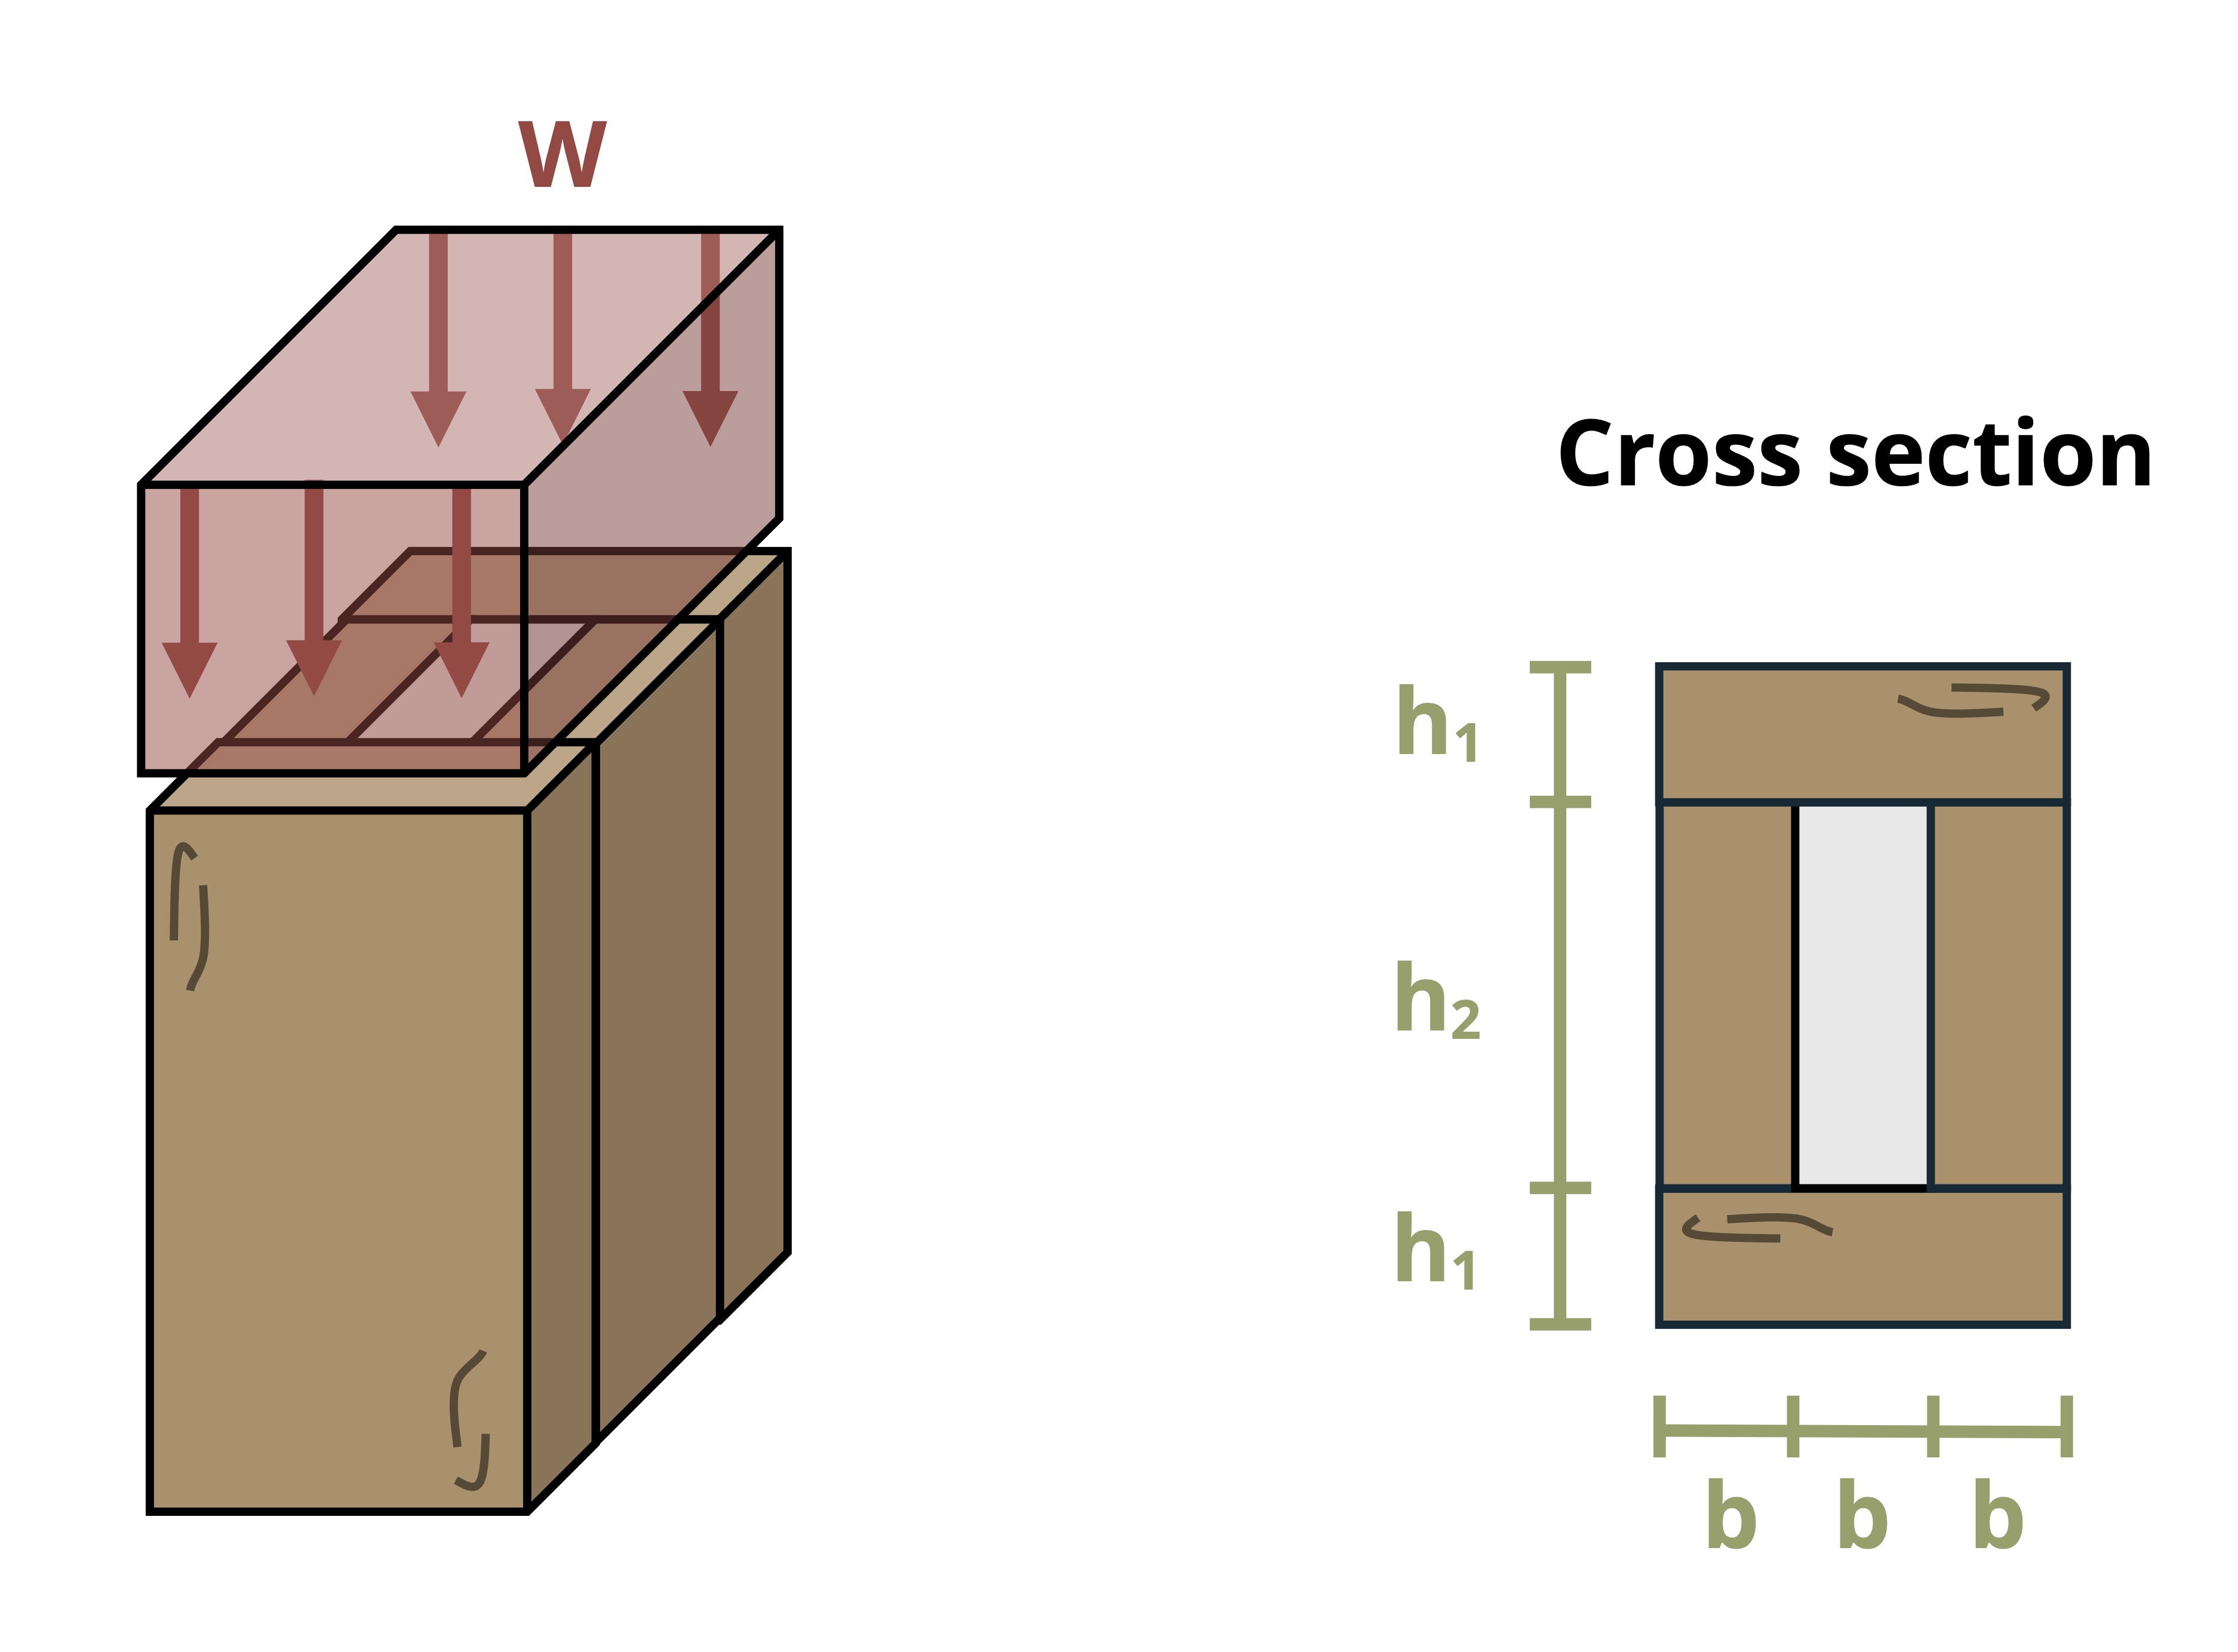
\includegraphics[keepaspectratio]{images/248.png}}
{[}Problem adapted from © Kurt Gramoll CC BY NC-SA 4.0{]}

\begin{Shaded}
\begin{Highlighting}[]
\NormalTok{\#| standalone: true}
\NormalTok{\#| viewerHeight: 600}
\NormalTok{\#| components: [viewer]}

\NormalTok{from shiny import App, render, ui, reactive}
\NormalTok{import random}
\NormalTok{import asyncio}
\NormalTok{import io}
\NormalTok{import math}
\NormalTok{import string}
\NormalTok{from datetime import datetime}
\NormalTok{from pathlib import Path}

\NormalTok{def generate\_random\_letters(length):}
\NormalTok{    \# Generate a random string of letters of specified length}
\NormalTok{    return \textquotesingle{}\textquotesingle{}.join(random.choice(string.ascii\_lowercase) for \_ in range(length)) }

\NormalTok{problem\_ID="248"}
\NormalTok{w=reactive.Value("\_\_")}
\NormalTok{b=reactive.Value("\_\_")}
\NormalTok{h1=reactive.Value("\_\_")}
\NormalTok{h2=reactive.Value("\_\_")}
\NormalTok{Econcrete=25}
\NormalTok{Ewood=12}

\NormalTok{attempts=["Timestamp,Attempt,Answer,Feedback\textbackslash{}n"]}

\NormalTok{app\_ui = ui.page\_fluid(}
\NormalTok{    ui.markdown("**Please enter your ID number from your instructor and click to generate your problem**"),}
\NormalTok{    ui.input\_text("ID","", placeholder="Enter ID Number Here"),}
\NormalTok{    ui.input\_action\_button("generate\_problem", "Generate Problem", class\_="btn{-}primary"),}
\NormalTok{    ui.markdown("**Problem Statement**"),}
\NormalTok{    ui.output\_ui("ui\_problem\_statement"),}
\NormalTok{    ui.input\_text("answer","Your Answer in units of kN", placeholder="Please enter your answer"),}
\NormalTok{    ui.input\_action\_button("submit", "Submit Answer", class\_="btn{-}primary"),}
\NormalTok{    ui.download\_button("download", "Download File to Submit", class\_="btn{-}success"),}
\NormalTok{)}


\NormalTok{def server(input, output, session):}
\NormalTok{    \# Initialize a counter for attempts}
\NormalTok{    attempt\_counter = reactive.Value(0)}

\NormalTok{    @output}
\NormalTok{    @render.ui}
\NormalTok{    def ui\_problem\_statement():}
\NormalTok{        return[ui.markdown(f"A distributed load w = \{w()\} N/cm\textless{}sup\textgreater{}2\textless{}/sup\textgreater{} is applied to a short column made from wood and concrete. Assume E\textless{}sub\textgreater{}concrete \textless{}/sub\textgreater{}= 25 GPa, E\textless{}sub\textgreater{}wood\textless{}/sub\textgreater{} = 12 GPa, b = \{b()\} cm, h\textless{}sub\textgreater{}1\textless{}/sub\textgreater{} = \{h1()\} cm, and h\textless{}sub\textgreater{}2\textless{}/sub\textgreater{} = \{h2()\} cm. What load is carried by the concrete center?")]}
    
\NormalTok{    @reactive.Effect}
\NormalTok{    @reactive.event(input.generate\_problem)}
\NormalTok{    def randomize\_vars():}
\NormalTok{        random.seed(input.ID())}
\NormalTok{        w.set(random.randrange(50, 750, 10))}
\NormalTok{        b.set(random.randrange(20, 100, 1)/10)}
\NormalTok{        h1.set(b()*1)}
\NormalTok{        h2.set(b()*2)}
        
\NormalTok{    @reactive.Effect}
\NormalTok{    @reactive.event(input.submit)}
\NormalTok{    def \_():}
\NormalTok{        attempt\_counter.set(attempt\_counter() + 1)  \# Increment the attempt counter on each submission.}
\NormalTok{        instr= (2.0833*h2()*w()*(2*h1()+h2())*3*b())/(6*h1()+4.0833*h2())/1000}
\NormalTok{        if math.isclose(float(input.answer()), instr, rel\_tol=0.01):}
\NormalTok{            check = "*Correct*"}
\NormalTok{            correct\_indicator = "JL"}
\NormalTok{        else:}
\NormalTok{            check = "*Not Correct.*"}
\NormalTok{            correct\_indicator = "JG"}

\NormalTok{        \# Generate random parts for the encoded attempt.}
\NormalTok{        random\_start = generate\_random\_letters(4)}
\NormalTok{        random\_middle = generate\_random\_letters(4)}
\NormalTok{        random\_end = generate\_random\_letters(4)}
\NormalTok{        encoded\_attempt = f"\{random\_start\}\{problem\_ID\}{-}\{random\_middle\}\{attempt\_counter()\}\{correct\_indicator\}{-}\{random\_end\}\{input.ID()\}"}

\NormalTok{        \# Store the most recent encoded attempt in a reactive value so it persists across submissions}
\NormalTok{        session.encoded\_attempt = reactive.Value(encoded\_attempt)}

\NormalTok{        \# Append the attempt data to the attempts list without the encoded attempt}
\NormalTok{        attempts.append(f"\{datetime.now()\}, \{attempt\_counter()\}, \{input.answer()\}, \{check\}\textbackslash{}n")}

\NormalTok{        \# Show feedback to the user.}
\NormalTok{        feedback = ui.markdown(f"Your answer of \{input.answer()\} is \{check\}.")}
\NormalTok{        m = ui.modal(}
\NormalTok{            feedback,}
\NormalTok{            title="Feedback",}
\NormalTok{            easy\_close=True}
\NormalTok{        )}
\NormalTok{        ui.modal\_show(m)}

\NormalTok{    @session.download(filename=lambda: f"Problem\_Log{-}\{problem\_ID\}{-}\{input.ID()\}.csv")}
\NormalTok{    async def download():}
\NormalTok{        \# Start the CSV with the encoded attempt (without label)}
\NormalTok{        final\_encoded = session.encoded\_attempt() if session.encoded\_attempt is not None else "No attempts"}
\NormalTok{        yield f"\{final\_encoded\}\textbackslash{}n\textbackslash{}n"}
        
\NormalTok{        \# Write the header for the remaining CSV data once}
\NormalTok{        yield "Timestamp,Attempt,Answer,Feedback\textbackslash{}n"}
        
\NormalTok{        \# Write the attempts data, ensure that the header from the attempts list is not written again}
\NormalTok{        for attempt in attempts[1:]:  \# Skip the first element which is the header}
\NormalTok{            await asyncio.sleep(0.25)  \# This delay may not be necessary; adjust as needed}
\NormalTok{            yield attempt}


\NormalTok{\# App installation}
\NormalTok{app = App(app\_ui, server)}
\end{Highlighting}
\end{Shaded}

\chapter*{Problem 5.39 - Statically Indeterminate Axial
Loads}\label{problem-5.39---statically-indeterminate-axial-loads}
\addcontentsline{toc}{chapter}{Problem 5.39 - Statically Indeterminate
Axial Loads}

\markboth{Problem 5.39 - Statically Indeterminate Axial Loads}{Problem
5.39 - Statically Indeterminate Axial Loads}

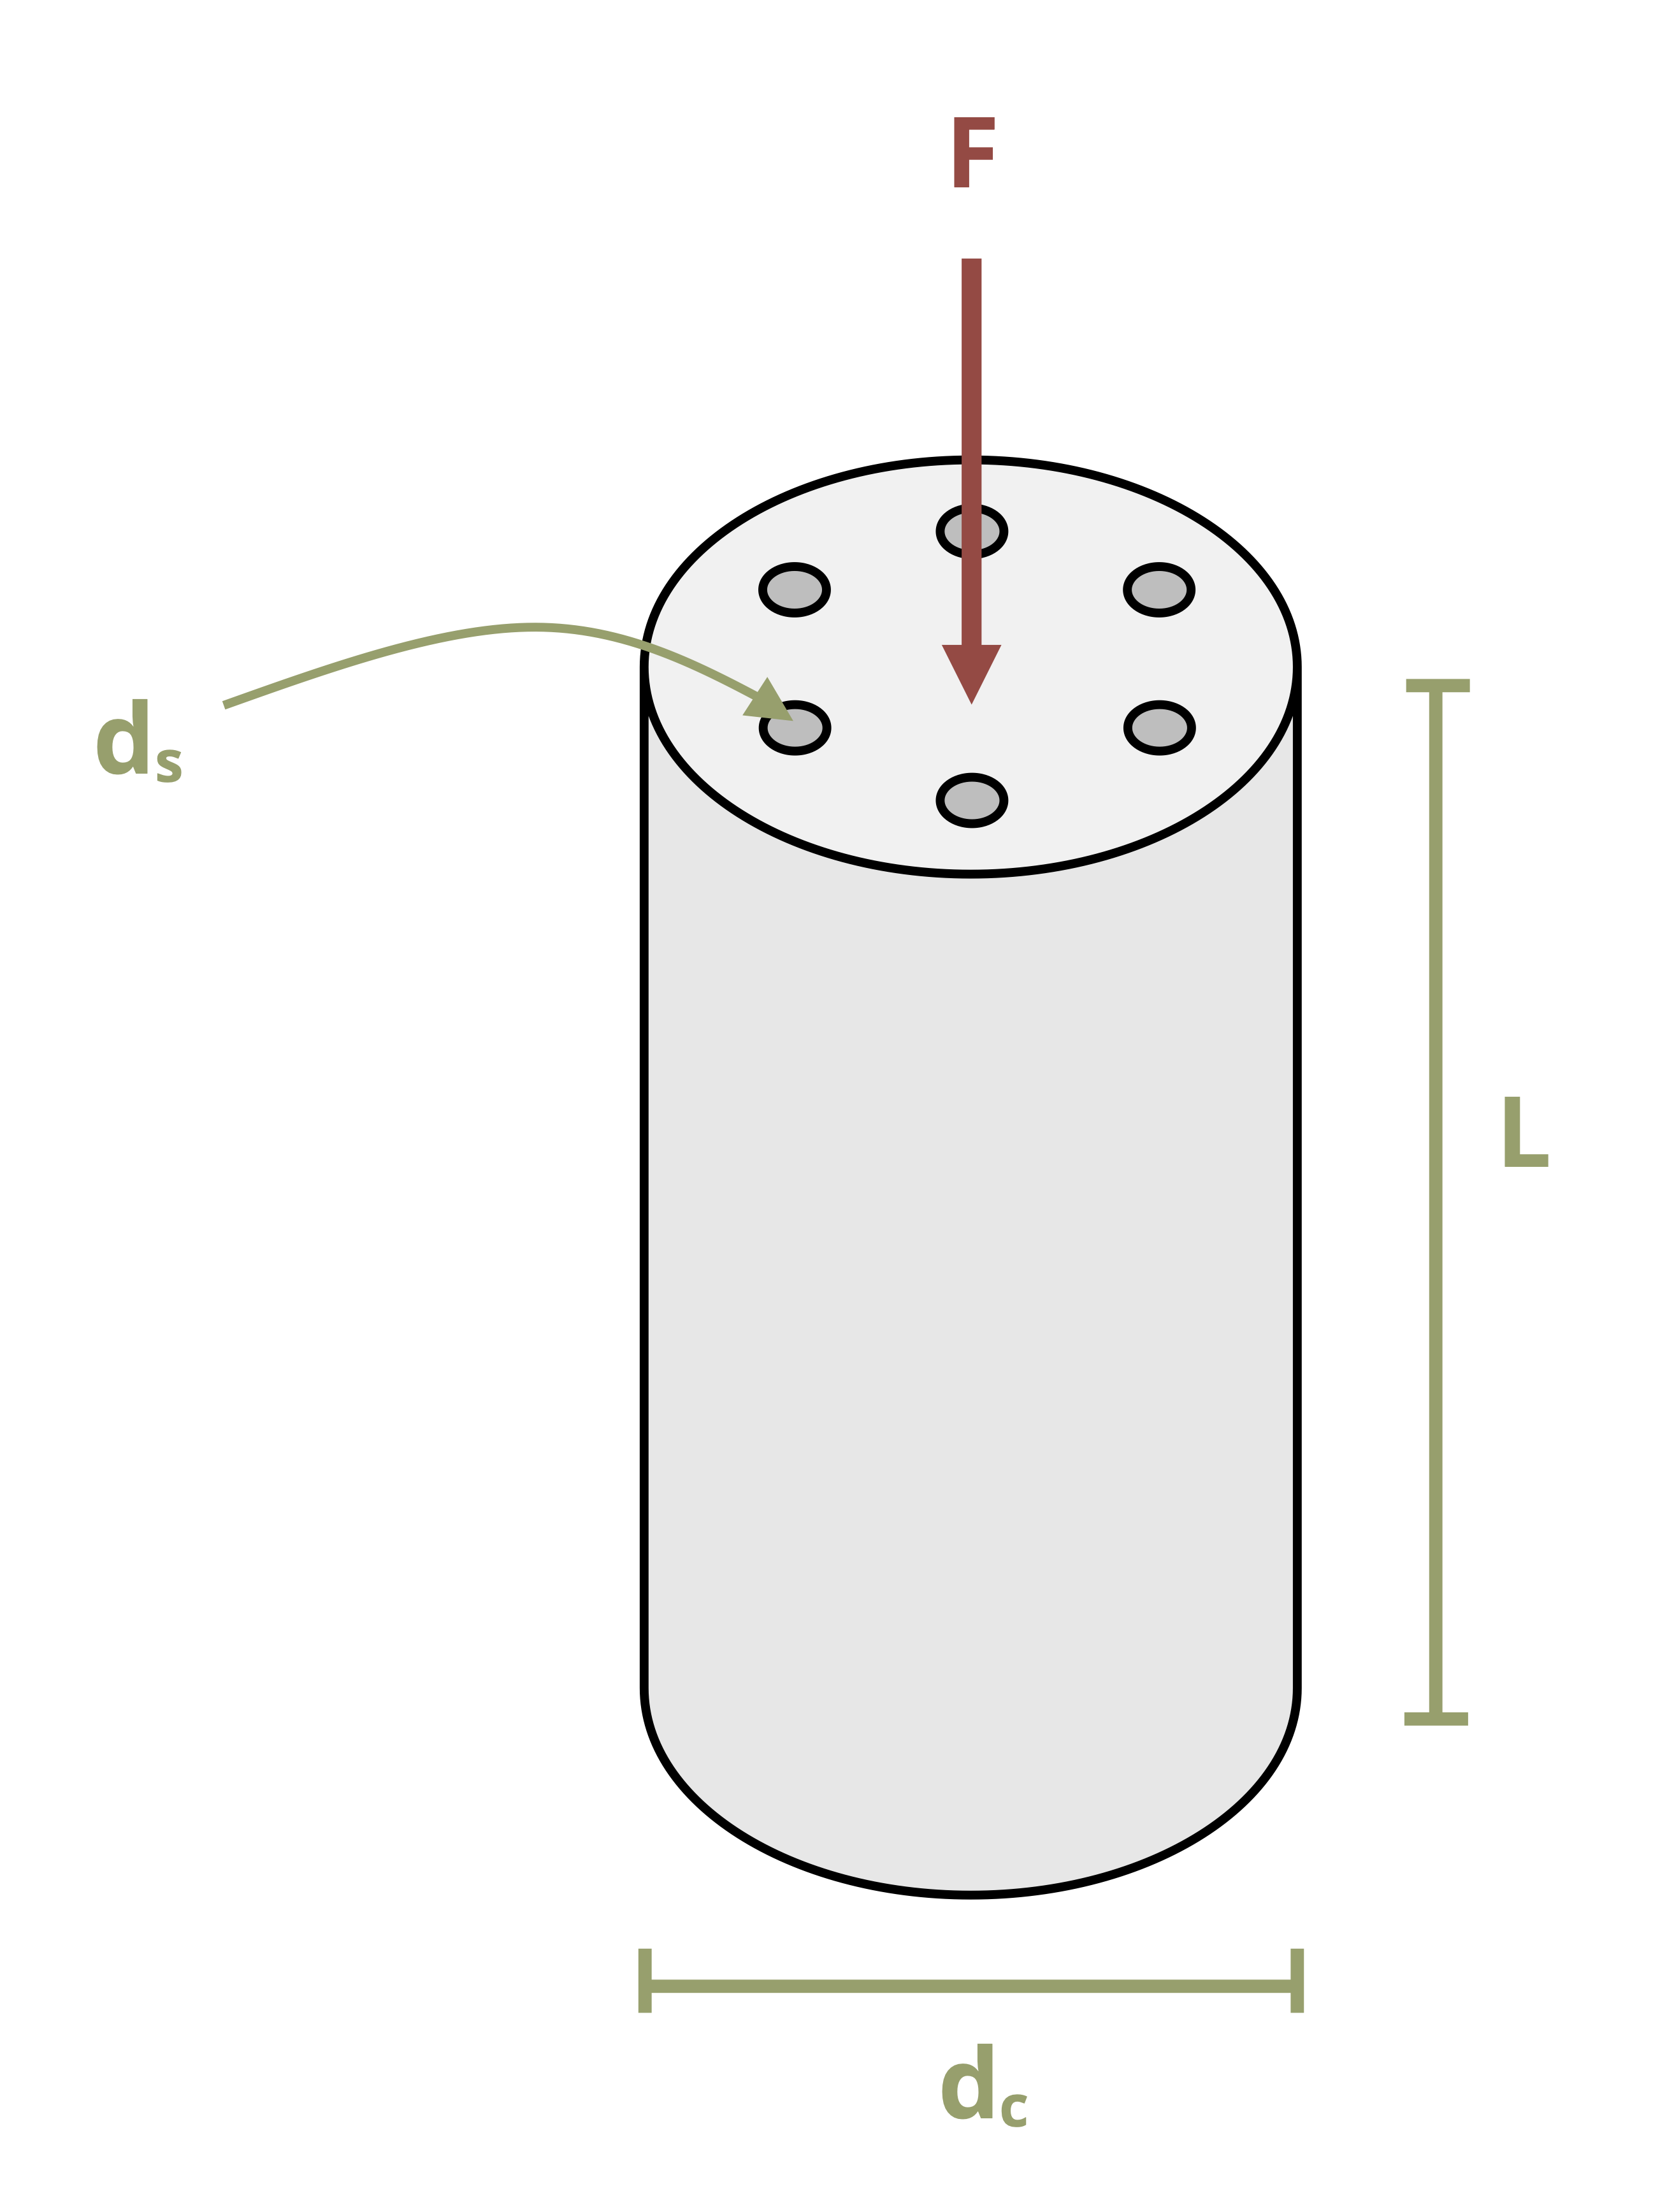
\includegraphics[width=2.60417in,height=\textheight,keepaspectratio]{images/250.png}
{[}Problem adapted from © Kurt Gramoll CC BY NC-SA 4.0{]}

\begin{Shaded}
\begin{Highlighting}[]
\NormalTok{\#| standalone: true}
\NormalTok{\#| viewerHeight: 600}
\NormalTok{\#| components: [viewer]}

\NormalTok{from shiny import App, render, ui, reactive}
\NormalTok{import random}
\NormalTok{import asyncio}
\NormalTok{import io}
\NormalTok{import math}
\NormalTok{import string}
\NormalTok{from datetime import datetime}
\NormalTok{from pathlib import Path}

\NormalTok{def generate\_random\_letters(length):}
\NormalTok{    \# Generate a random string of letters of specified length}
\NormalTok{    return \textquotesingle{}\textquotesingle{}.join(random.choice(string.ascii\_lowercase) for \_ in range(length)) }

\NormalTok{problem\_ID="250"}
\NormalTok{F=reactive.Value("\_\_")}
\NormalTok{L=reactive.Value("\_\_")}
\NormalTok{dc=reactive.Value("\_\_")}
\NormalTok{ds=reactive.Value("\_\_")}
\NormalTok{Econcrete=25}
\NormalTok{Esteel=200}

\NormalTok{attempts=["Timestamp,Attempt,Answer,Feedback\textbackslash{}n"]}

\NormalTok{app\_ui = ui.page\_fluid(}
\NormalTok{    ui.markdown("**Please enter your ID number from your instructor and click to generate your problem**"),}
\NormalTok{    ui.input\_text("ID","", placeholder="Enter ID Number Here"),}
\NormalTok{    ui.input\_action\_button("generate\_problem", "Generate Problem", class\_="btn{-}primary"),}
\NormalTok{    ui.markdown("**Problem Statement**"),}
\NormalTok{    ui.output\_ui("ui\_problem\_statement"),}
\NormalTok{    ui.input\_text("answer","Your Answer in units of MPa", placeholder="Please enter your answer"),}
\NormalTok{    ui.input\_action\_button("submit", "Submit Answer", class\_="btn{-}primary"),}
\NormalTok{    ui.download\_button("download", "Download File to Submit", class\_="btn{-}success"),}
\NormalTok{)}


\NormalTok{def server(input, output, session):}
\NormalTok{    \# Initialize a counter for attempts}
\NormalTok{    attempt\_counter = reactive.Value(0)}

\NormalTok{    @output}
\NormalTok{    @render.ui}
\NormalTok{    def ui\_problem\_statement():}
\NormalTok{        return[ui.markdown(f"A concrete post of length L = \{L()\}  m and diameter d\textless{}sub\textgreater{}c\textless{}/sub\textgreater{} = \{dc()\} mm supports a load F = \{F()\} kN. The concrete is reinforced with 6 steel rods of diameter d\textless{}sub\textgreater{}s\textless{}/sub\textgreater{} = \{ds()\} mm. Assume E\textless{}sub\textgreater{}concrete\textless{}/sub\textgreater{} = 25 GPa and E\textless{}sub\textgreater{}steel\textless{}/sub\textgreater{} = 200 GPa. Determine the stress in the concrete.")]}
    
\NormalTok{    @reactive.Effect}
\NormalTok{    @reactive.event(input.generate\_problem)}
\NormalTok{    def randomize\_vars():}
\NormalTok{        random.seed(input.ID())}
\NormalTok{        L.set(random.randrange(10, 50, 1)/10)}
\NormalTok{        dc.set(random.randrange(100, 500, 10))}
\NormalTok{        ds.set(round(dc()/12))}
\NormalTok{        F.set(random.randrange(100, 500, 10))}
        
\NormalTok{    @reactive.Effect}
\NormalTok{    @reactive.event(input.submit)}
\NormalTok{    def \_():}
\NormalTok{        attempt\_counter.set(attempt\_counter() + 1)  \# Increment the attempt counter on each submission.}
\NormalTok{        As = (math.pi*6*(ds()/20)**2)}
\NormalTok{        Ac = (math.pi*(dc()/20)**2) {-} As}
\NormalTok{        Cside = Ac*Econcrete}
\NormalTok{        Sside = As*Esteel}
\NormalTok{        LHS = F()*Cside}
\NormalTok{        RHS = Cside+Sside}
\NormalTok{        instr= ((LHS/RHS)/(Ac/100**2))/10**3}
\NormalTok{        if math.isclose(float(input.answer()), instr, rel\_tol=0.01):}
\NormalTok{            check = "*Correct*"}
\NormalTok{            correct\_indicator = "JL"}
\NormalTok{        else:}
\NormalTok{            check = "*Not Correct.*"}
\NormalTok{            correct\_indicator = "JG"}

\NormalTok{        \# Generate random parts for the encoded attempt.}
\NormalTok{        random\_start = generate\_random\_letters(4)}
\NormalTok{        random\_middle = generate\_random\_letters(4)}
\NormalTok{        random\_end = generate\_random\_letters(4)}
\NormalTok{        encoded\_attempt = f"\{random\_start\}\{problem\_ID\}{-}\{random\_middle\}\{attempt\_counter()\}\{correct\_indicator\}{-}\{random\_end\}\{input.ID()\}"}

\NormalTok{        \# Store the most recent encoded attempt in a reactive value so it persists across submissions}
\NormalTok{        session.encoded\_attempt = reactive.Value(encoded\_attempt)}

\NormalTok{        \# Append the attempt data to the attempts list without the encoded attempt}
\NormalTok{        attempts.append(f"\{datetime.now()\}, \{attempt\_counter()\}, \{input.answer()\}, \{check\}\textbackslash{}n")}

\NormalTok{        \# Show feedback to the user.}
\NormalTok{        feedback = ui.markdown(f"Your answer of \{input.answer()\} is \{check\}.")}
\NormalTok{        m = ui.modal(}
\NormalTok{            feedback,}
\NormalTok{            title="Feedback",}
\NormalTok{            easy\_close=True}
\NormalTok{        )}
\NormalTok{        ui.modal\_show(m)}

\NormalTok{    @session.download(filename=lambda: f"Problem\_Log{-}\{problem\_ID\}{-}\{input.ID()\}.csv")}
\NormalTok{    async def download():}
\NormalTok{        \# Start the CSV with the encoded attempt (without label)}
\NormalTok{        final\_encoded = session.encoded\_attempt() if session.encoded\_attempt is not None else "No attempts"}
\NormalTok{        yield f"\{final\_encoded\}\textbackslash{}n\textbackslash{}n"}
        
\NormalTok{        \# Write the header for the remaining CSV data once}
\NormalTok{        yield "Timestamp,Attempt,Answer,Feedback\textbackslash{}n"}
        
\NormalTok{        \# Write the attempts data, ensure that the header from the attempts list is not written again}
\NormalTok{        for attempt in attempts[1:]:  \# Skip the first element which is the header}
\NormalTok{            await asyncio.sleep(0.25)  \# This delay may not be necessary; adjust as needed}
\NormalTok{            yield attempt}


\NormalTok{\# App installation}
\NormalTok{app = App(app\_ui, server)}
\end{Highlighting}
\end{Shaded}

\chapter*{Problem 5.50 - Thermal
Deformation}\label{problem-5.50---thermal-deformation}
\addcontentsline{toc}{chapter}{Problem 5.50 - Thermal Deformation}

\markboth{Problem 5.50 - Thermal Deformation}{Problem 5.50 - Thermal
Deformation}

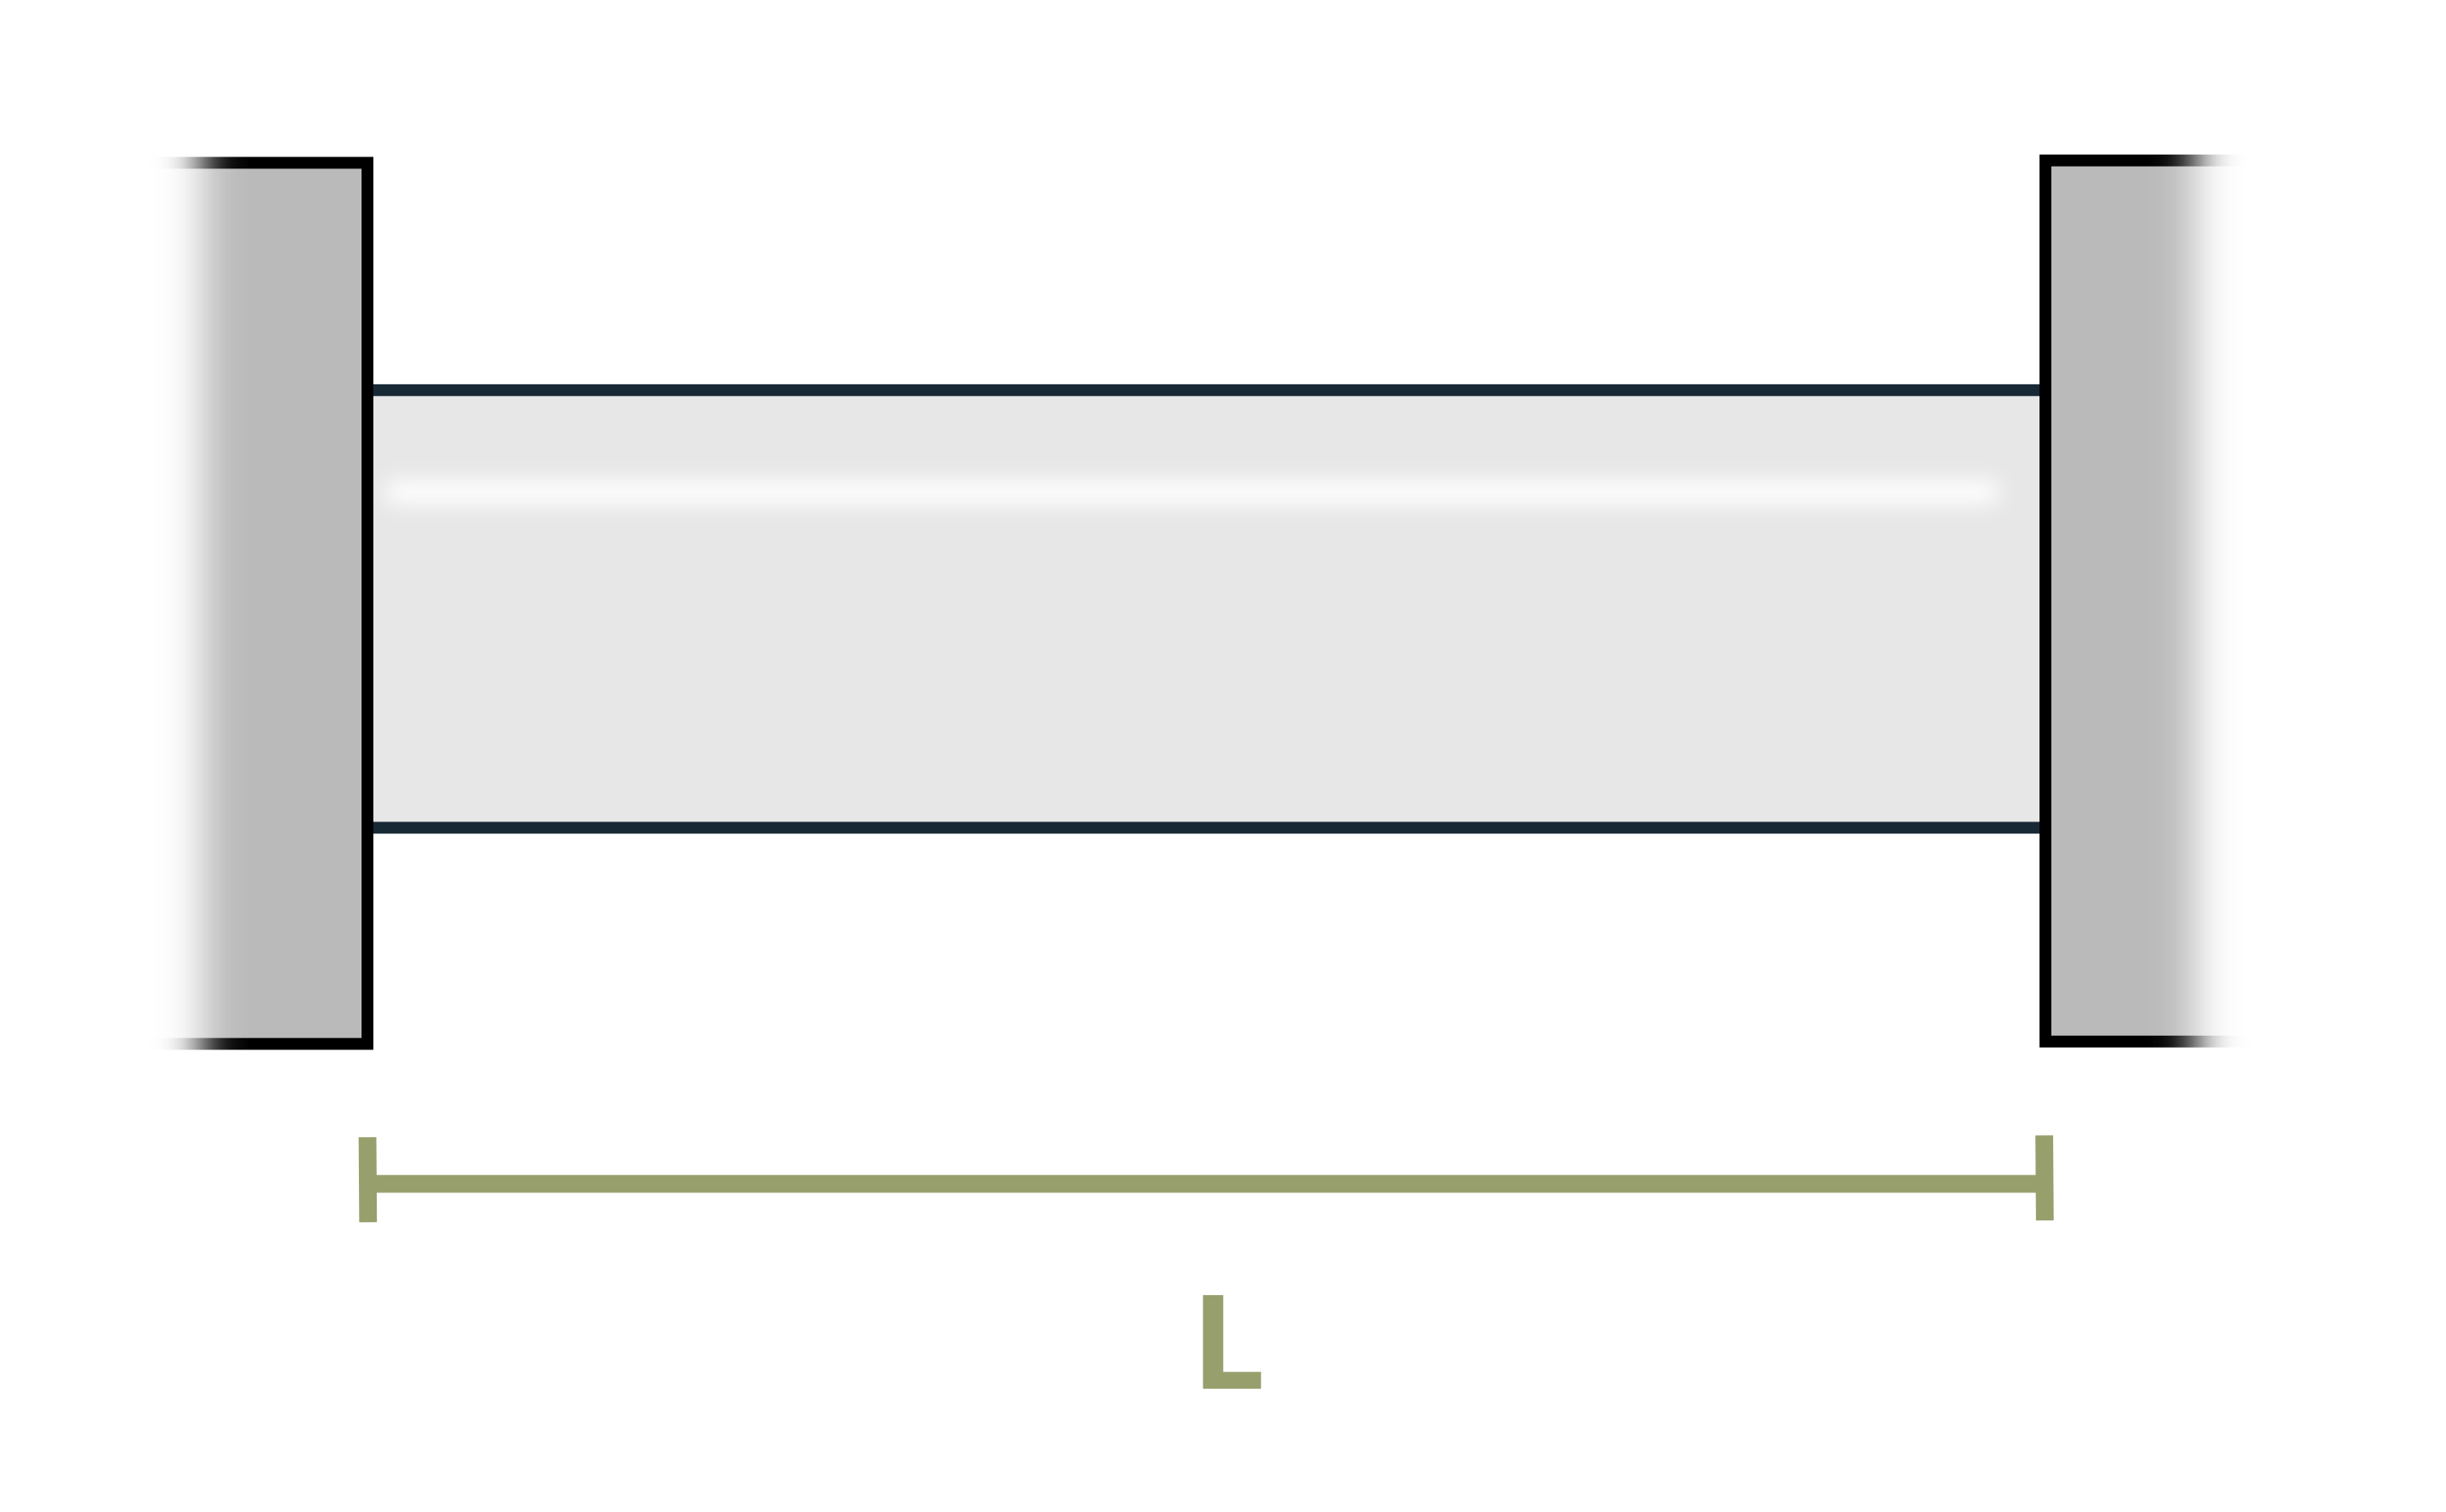
\includegraphics[width=3.125in,height=\textheight,keepaspectratio]{images/222.png}
{[}Problem adapted from © Kurt Gramoll CC BY NC-SA 4.0{]}

\begin{Shaded}
\begin{Highlighting}[]
\NormalTok{\#| standalone: true}
\NormalTok{\#| viewerHeight: 600}
\NormalTok{\#| components: [viewer]}

\NormalTok{from shiny import App, render, ui, reactive}
\NormalTok{import random}
\NormalTok{import asyncio}
\NormalTok{import io}
\NormalTok{import math}
\NormalTok{import string}
\NormalTok{from datetime import datetime}
\NormalTok{from pathlib import Path}

\NormalTok{def generate\_random\_letters(length):}
\NormalTok{    \# Generate a random string of letters of specified length}
\NormalTok{    return \textquotesingle{}\textquotesingle{}.join(random.choice(string.ascii\_lowercase) for \_ in range(length)) }

\NormalTok{problem\_ID="222"}
\NormalTok{stress=reactive.Value("\_\_")}
\NormalTok{L=reactive.Value("\_\_")}
\NormalTok{E=29000}
\NormalTok{alpha=6.5*10**{-}6}

\NormalTok{attempts=["Timestamp,Attempt,Answer,Feedback\textbackslash{}n"]}

\NormalTok{app\_ui = ui.page\_fluid(}
\NormalTok{    ui.markdown("**Please enter your ID number from your instructor and click to generate your problem**"),}
\NormalTok{    ui.input\_text("ID","", placeholder="Enter ID Number Here"),}
\NormalTok{    ui.input\_action\_button("generate\_problem", "Generate Problem", class\_="btn{-}primary"),}
\NormalTok{    ui.markdown("**Problem Statement**"),}
\NormalTok{    ui.output\_ui("ui\_problem\_statement"),}
\NormalTok{    ui.input\_text("answer","Your Answer in units of °F", placeholder="Please enter your answer"),}
\NormalTok{    ui.input\_action\_button("submit", "Submit Answer", class\_="btn{-}primary"),}
\NormalTok{    ui.download\_button("download", "Download File to Submit", class\_="btn{-}success"),}
\NormalTok{)}


\NormalTok{def server(input, output, session):}
\NormalTok{    \# Initialize a counter for attempts}
\NormalTok{    attempt\_counter = reactive.Value(0)}

\NormalTok{    @output}
\NormalTok{    @render.ui}
\NormalTok{    def ui\_problem\_statement():}
\NormalTok{        return[ui.markdown(f"The axial stress in a solid circular bar between two fixed walls is \{stress()\} ksi. Find the temperature change necessary to relieve the stress. Assume L = \{L()\} in., E = 29,000 ksi, and α = 6.5 x 10\textless{}sup\textgreater{}{-}6\textless{}/sup\textgreater{} / °F. ")]}
    
\NormalTok{    @reactive.Effect}
\NormalTok{    @reactive.event(input.generate\_problem)}
\NormalTok{    def randomize\_vars():}
\NormalTok{        random.seed(input.ID())}
\NormalTok{        stress.set(random.randrange(10, 150, 5))}
\NormalTok{        L.set(random.randrange(15, 75, 1))}
        
\NormalTok{    @reactive.Effect}
\NormalTok{    @reactive.event(input.submit)}
\NormalTok{    def \_():}
\NormalTok{        attempt\_counter.set(attempt\_counter() + 1)  \# Increment the attempt counter on each submission.}
\NormalTok{        instr= stress()/(alpha*E)}
\NormalTok{        if math.isclose(float(input.answer()), instr, rel\_tol=0.01):}
\NormalTok{            check = "*Correct*"}
\NormalTok{            correct\_indicator = "JL"}
\NormalTok{        else:}
\NormalTok{            check = "*Not Correct.*"}
\NormalTok{            correct\_indicator = "JG"}

\NormalTok{        \# Generate random parts for the encoded attempt.}
\NormalTok{        random\_start = generate\_random\_letters(4)}
\NormalTok{        random\_middle = generate\_random\_letters(4)}
\NormalTok{        random\_end = generate\_random\_letters(4)}
\NormalTok{        encoded\_attempt = f"\{random\_start\}\{problem\_ID\}{-}\{random\_middle\}\{attempt\_counter()\}\{correct\_indicator\}{-}\{random\_end\}\{input.ID()\}"}

\NormalTok{        \# Store the most recent encoded attempt in a reactive value so it persists across submissions}
\NormalTok{        session.encoded\_attempt = reactive.Value(encoded\_attempt)}

\NormalTok{        \# Append the attempt data to the attempts list without the encoded attempt}
\NormalTok{        attempts.append(f"\{datetime.now()\}, \{attempt\_counter()\}, \{input.answer()\}, \{check\}\textbackslash{}n")}

\NormalTok{        \# Show feedback to the user.}
\NormalTok{        feedback = ui.markdown(f"Your answer of \{input.answer()\} is \{check\}.")}
\NormalTok{        m = ui.modal(}
\NormalTok{            feedback,}
\NormalTok{            title="Feedback",}
\NormalTok{            easy\_close=True}
\NormalTok{        )}
\NormalTok{        ui.modal\_show(m)}

\NormalTok{    @session.download(filename=lambda: f"Problem\_Log{-}\{problem\_ID\}{-}\{input.ID()\}.csv")}
\NormalTok{    async def download():}
\NormalTok{        \# Start the CSV with the encoded attempt (without label)}
\NormalTok{        final\_encoded = session.encoded\_attempt() if session.encoded\_attempt is not None else "No attempts"}
\NormalTok{        yield f"\{final\_encoded\}\textbackslash{}n\textbackslash{}n"}
        
\NormalTok{        \# Write the header for the remaining CSV data once}
\NormalTok{        yield "Timestamp,Attempt,Answer,Feedback\textbackslash{}n"}
        
\NormalTok{        \# Write the attempts data, ensure that the header from the attempts list is not written again}
\NormalTok{        for attempt in attempts[1:]:  \# Skip the first element which is the header}
\NormalTok{            await asyncio.sleep(0.25)  \# This delay may not be necessary; adjust as needed}
\NormalTok{            yield attempt}


\NormalTok{\# App installation}
\NormalTok{app = App(app\_ui, server)}
\end{Highlighting}
\end{Shaded}

\chapter*{Problem 5.51 - Thermal
Deformation}\label{problem-5.51---thermal-deformation}
\addcontentsline{toc}{chapter}{Problem 5.51 - Thermal Deformation}

\markboth{Problem 5.51 - Thermal Deformation}{Problem 5.51 - Thermal
Deformation}

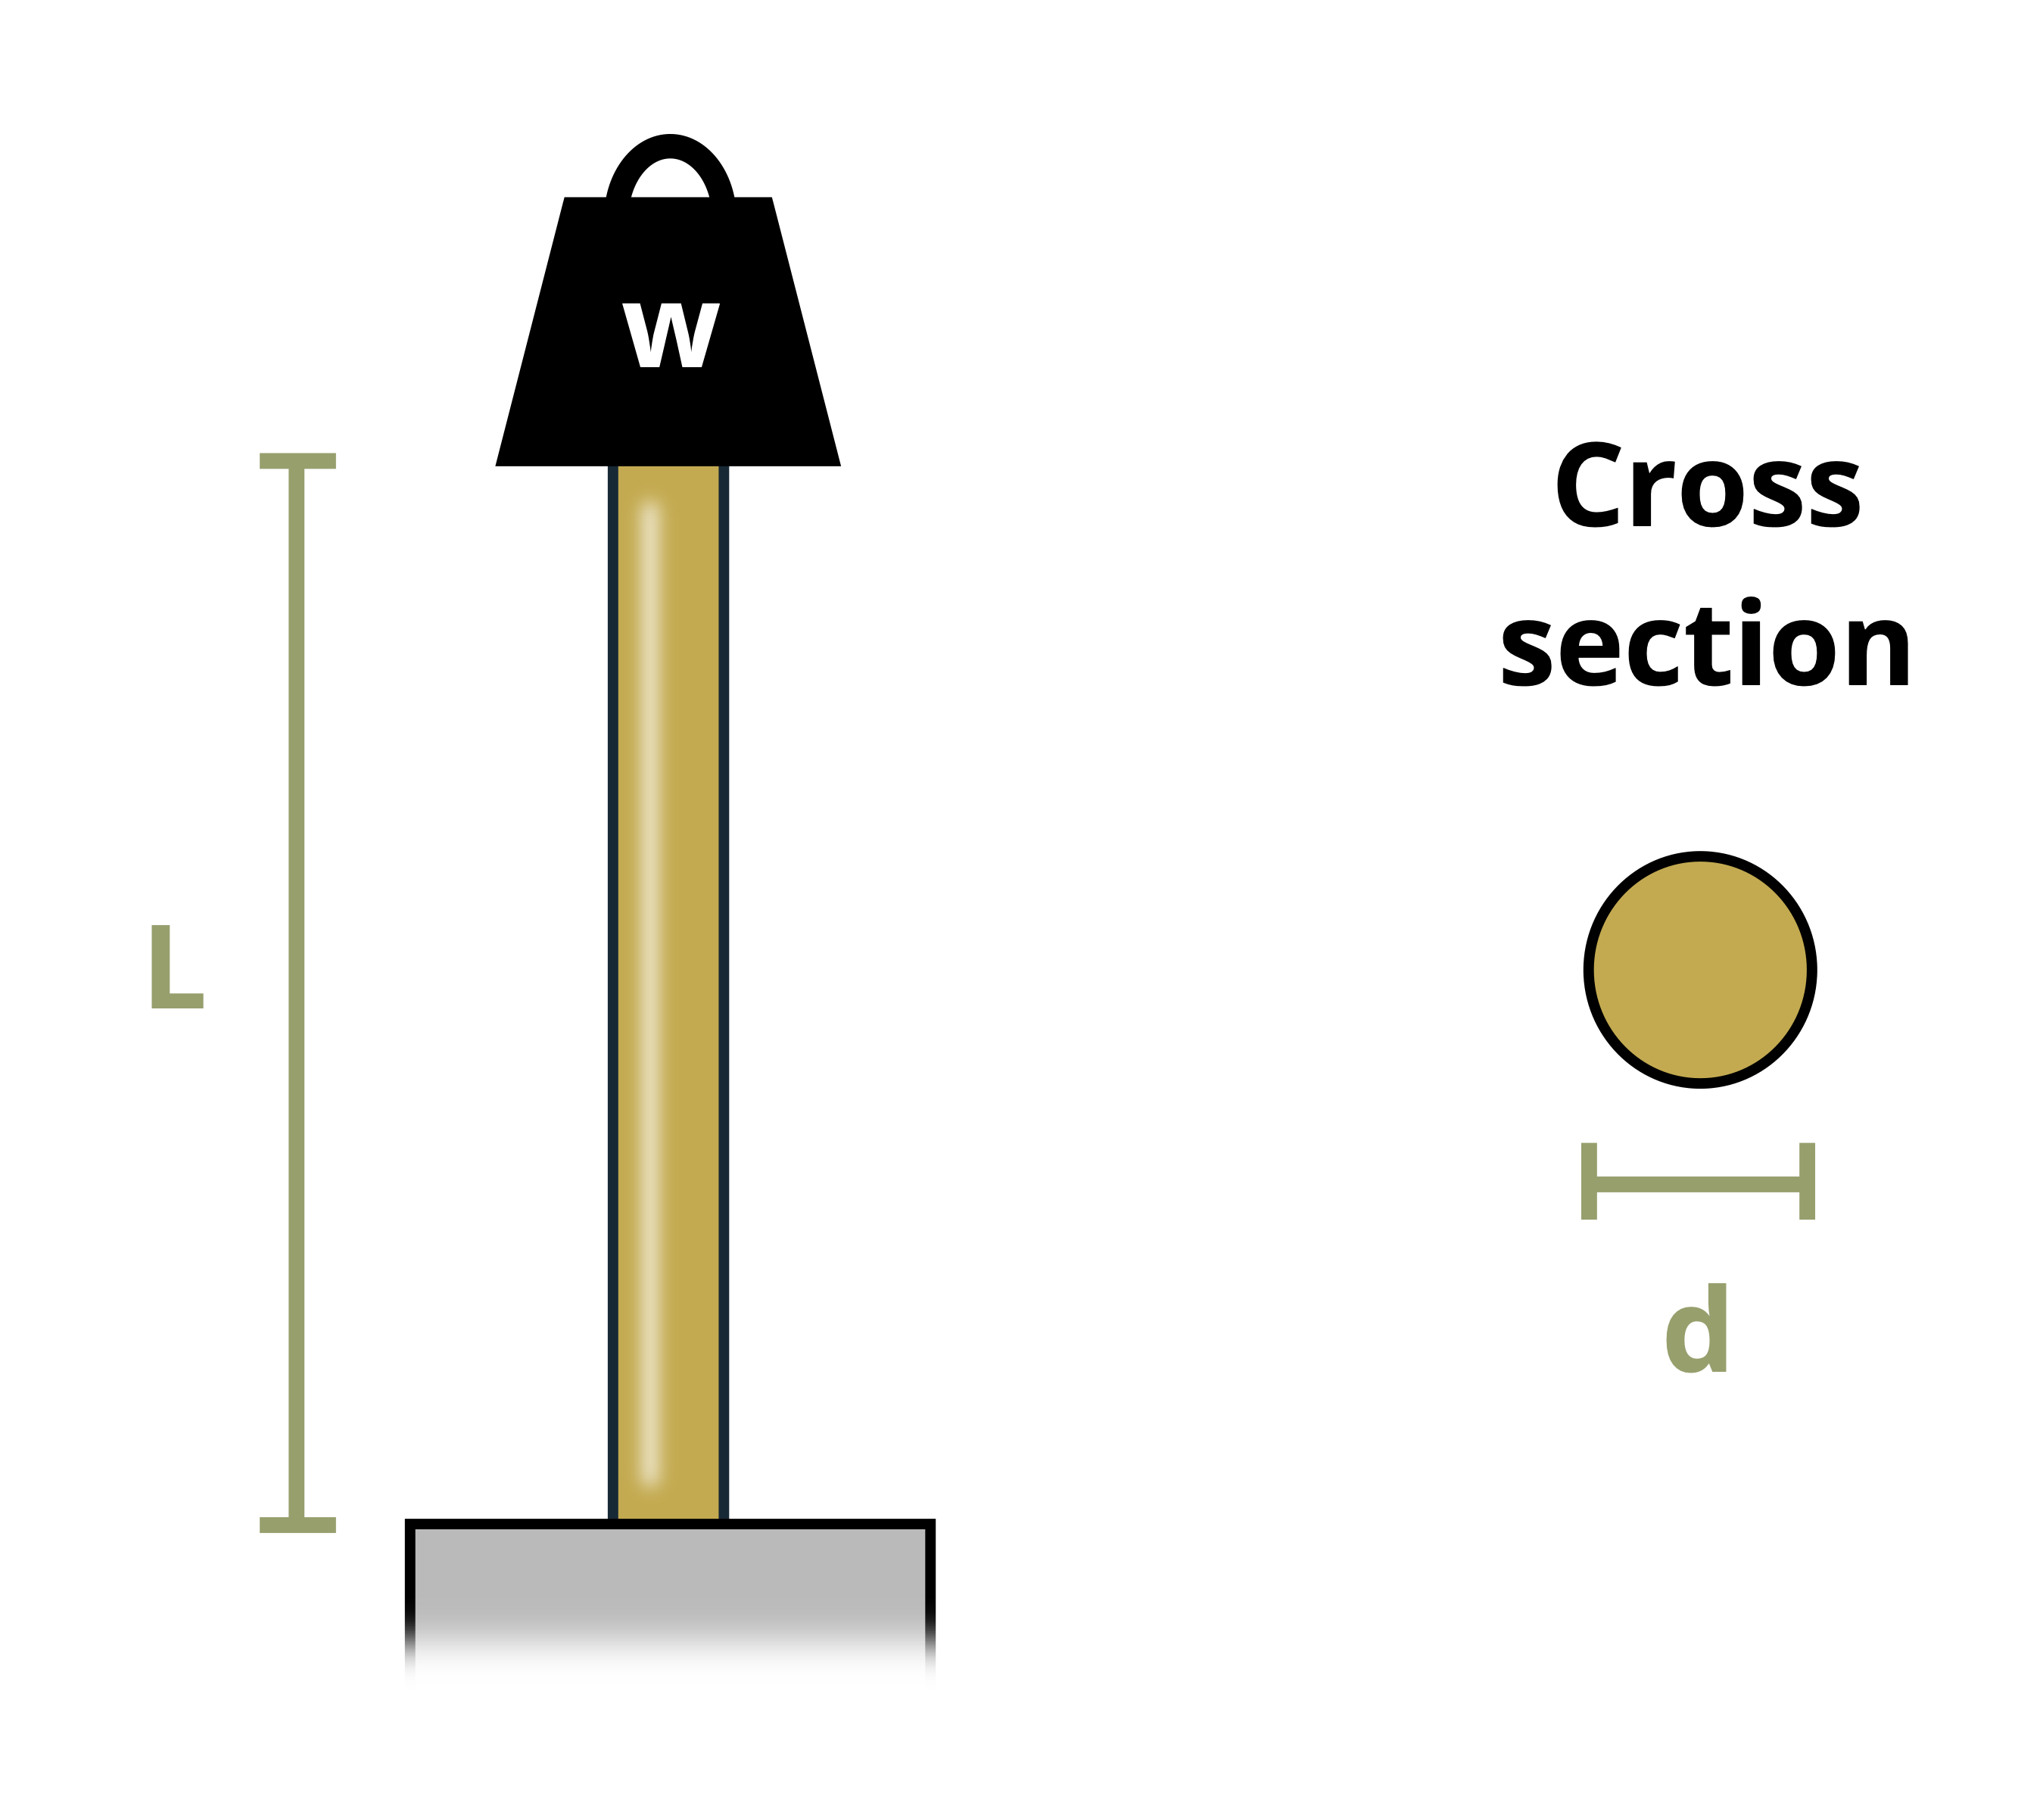
\includegraphics[width=3.125in,height=\textheight,keepaspectratio]{images/223.png}
{[}Problem adapted from © Kurt Gramoll CC BY NC-SA 4.0{]}

\begin{Shaded}
\begin{Highlighting}[]
\NormalTok{\#| standalone: true}
\NormalTok{\#| viewerHeight: 600}
\NormalTok{\#| components: [viewer]}

\NormalTok{from shiny import App, render, ui, reactive}
\NormalTok{import random}
\NormalTok{import asyncio}
\NormalTok{import io}
\NormalTok{import math}
\NormalTok{import string}
\NormalTok{from datetime import datetime}
\NormalTok{from pathlib import Path}

\NormalTok{def generate\_random\_letters(length):}
\NormalTok{    \# Generate a random string of letters of specified length}
\NormalTok{    return \textquotesingle{}\textquotesingle{}.join(random.choice(string.ascii\_lowercase) for \_ in range(length)) }

\NormalTok{problem\_ID="223"}
\NormalTok{W=reactive.Value("\_\_")}
\NormalTok{d=reactive.Value("\_\_")}
\NormalTok{L=reactive.Value("\_\_")}
\NormalTok{TC=reactive.Value("\_\_")}
\NormalTok{E=100*10**9}
\NormalTok{alpha=10*10**{-}6}

\NormalTok{attempts=["Timestamp,Attempt,Answer,Feedback\textbackslash{}n"]}

\NormalTok{app\_ui = ui.page\_fluid(}
\NormalTok{    ui.markdown("**Please enter your ID number from your instructor and click to generate your problem**"),}
\NormalTok{    ui.input\_text("ID","", placeholder="Enter ID Number Here"),}
\NormalTok{    ui.input\_action\_button("generate\_problem", "Generate Problem", class\_="btn{-}primary"),}
\NormalTok{    ui.markdown("**Problem Statement**"),}
\NormalTok{    ui.output\_ui("ui\_problem\_statement"),}
\NormalTok{    ui.input\_text("answer","Your Answer in units of mm", placeholder="Please enter your answer"),}
\NormalTok{    ui.input\_action\_button("submit", "Submit Answer", class\_="btn{-}primary"),}
\NormalTok{    ui.download\_button("download", "Download File to Submit", class\_="btn{-}success"),}
\NormalTok{)}


\NormalTok{def server(input, output, session):}
\NormalTok{    \# Initialize a counter for attempts}
\NormalTok{    attempt\_counter = reactive.Value(0)}

\NormalTok{    @output}
\NormalTok{    @render.ui}
\NormalTok{    def ui\_problem\_statement():}
\NormalTok{        return[ui.markdown(f"The W = \{W()\} kg weight is placed on a L = \{L()\} m tall brass bar with a cross section of d = \{d()\} cm. If the bar undergoes a temperature change of \{TC()\}°C, what is the total deformation of the bar? Assume the Young\textquotesingle{}s Modulus and thermal coefficient of expansion is 100 GPa and 10 x 10\textless{}sup\textgreater{}{-}6\textless{}/sup\textgreater{} /°C, respectively. Also, assume no buckling. ")]}
    
\NormalTok{    @reactive.Effect}
\NormalTok{    @reactive.event(input.generate\_problem)}
\NormalTok{    def randomize\_vars():}
\NormalTok{        random.seed(input.ID())}
\NormalTok{        W.set(random.randrange(500, 2000, 100))}
\NormalTok{        L.set(random.randrange(10, 50, 1)/10)}
\NormalTok{        d.set(random.randrange(15, 40, 1)/10)}
\NormalTok{        TC.set(random.randrange(20, 150, 5))}
        
        
\NormalTok{    @reactive.Effect}
\NormalTok{    @reactive.event(input.submit)}
\NormalTok{    def \_():}
\NormalTok{        attempt\_counter.set(attempt\_counter() + 1)  \# Increment the attempt counter on each submission.}
\NormalTok{        deltaT = L()*alpha*TC()}
\NormalTok{        deltaM = (W()*9.81*L())/(E*math.pi*(d()/200)**2) \#200 converts from diameter in cm to r in meters}
\NormalTok{        instr= (deltaT {-} deltaM)*1000 \# *1000 to get answer in mm}
\NormalTok{        if math.isclose(float(input.answer()), instr, rel\_tol=0.01):}
\NormalTok{            check = "*Correct*"}
\NormalTok{            correct\_indicator = "JL"}
\NormalTok{        else:}
\NormalTok{            check = "*Not Correct.*"}
\NormalTok{            correct\_indicator = "JG"}

\NormalTok{        \# Generate random parts for the encoded attempt.}
\NormalTok{        random\_start = generate\_random\_letters(4)}
\NormalTok{        random\_middle = generate\_random\_letters(4)}
\NormalTok{        random\_end = generate\_random\_letters(4)}
\NormalTok{        encoded\_attempt = f"\{random\_start\}\{problem\_ID\}{-}\{random\_middle\}\{attempt\_counter()\}\{correct\_indicator\}{-}\{random\_end\}\{input.ID()\}"}

\NormalTok{        \# Store the most recent encoded attempt in a reactive value so it persists across submissions}
\NormalTok{        session.encoded\_attempt = reactive.Value(encoded\_attempt)}

\NormalTok{        \# Append the attempt data to the attempts list without the encoded attempt}
\NormalTok{        attempts.append(f"\{datetime.now()\}, \{attempt\_counter()\}, \{input.answer()\}, \{check\}\textbackslash{}n")}

\NormalTok{        \# Show feedback to the user.}
\NormalTok{        feedback = ui.markdown(f"Your answer of \{input.answer()\} is \{check\}.")}
\NormalTok{        m = ui.modal(}
\NormalTok{            feedback,}
\NormalTok{            title="Feedback",}
\NormalTok{            easy\_close=True}
\NormalTok{        )}
\NormalTok{        ui.modal\_show(m)}

\NormalTok{    @session.download(filename=lambda: f"Problem\_Log{-}\{problem\_ID\}{-}\{input.ID()\}.csv")}
\NormalTok{    async def download():}
\NormalTok{        \# Start the CSV with the encoded attempt (without label)}
\NormalTok{        final\_encoded = session.encoded\_attempt() if session.encoded\_attempt is not None else "No attempts"}
\NormalTok{        yield f"\{final\_encoded\}\textbackslash{}n\textbackslash{}n"}
        
\NormalTok{        \# Write the header for the remaining CSV data once}
\NormalTok{        yield "Timestamp,Attempt,Answer,Feedback\textbackslash{}n"}
        
\NormalTok{        \# Write the attempts data, ensure that the header from the attempts list is not written again}
\NormalTok{        for attempt in attempts[1:]:  \# Skip the first element which is the header}
\NormalTok{            await asyncio.sleep(0.25)  \# This delay may not be necessary; adjust as needed}
\NormalTok{            yield attempt}


\NormalTok{\# App installation}
\NormalTok{app = App(app\_ui, server)}
\end{Highlighting}
\end{Shaded}

\chapter*{Problem 5.52 - Thermal
Deformation}\label{problem-5.52---thermal-deformation}
\addcontentsline{toc}{chapter}{Problem 5.52 - Thermal Deformation}

\markboth{Problem 5.52 - Thermal Deformation}{Problem 5.52 - Thermal
Deformation}

\pandocbounded{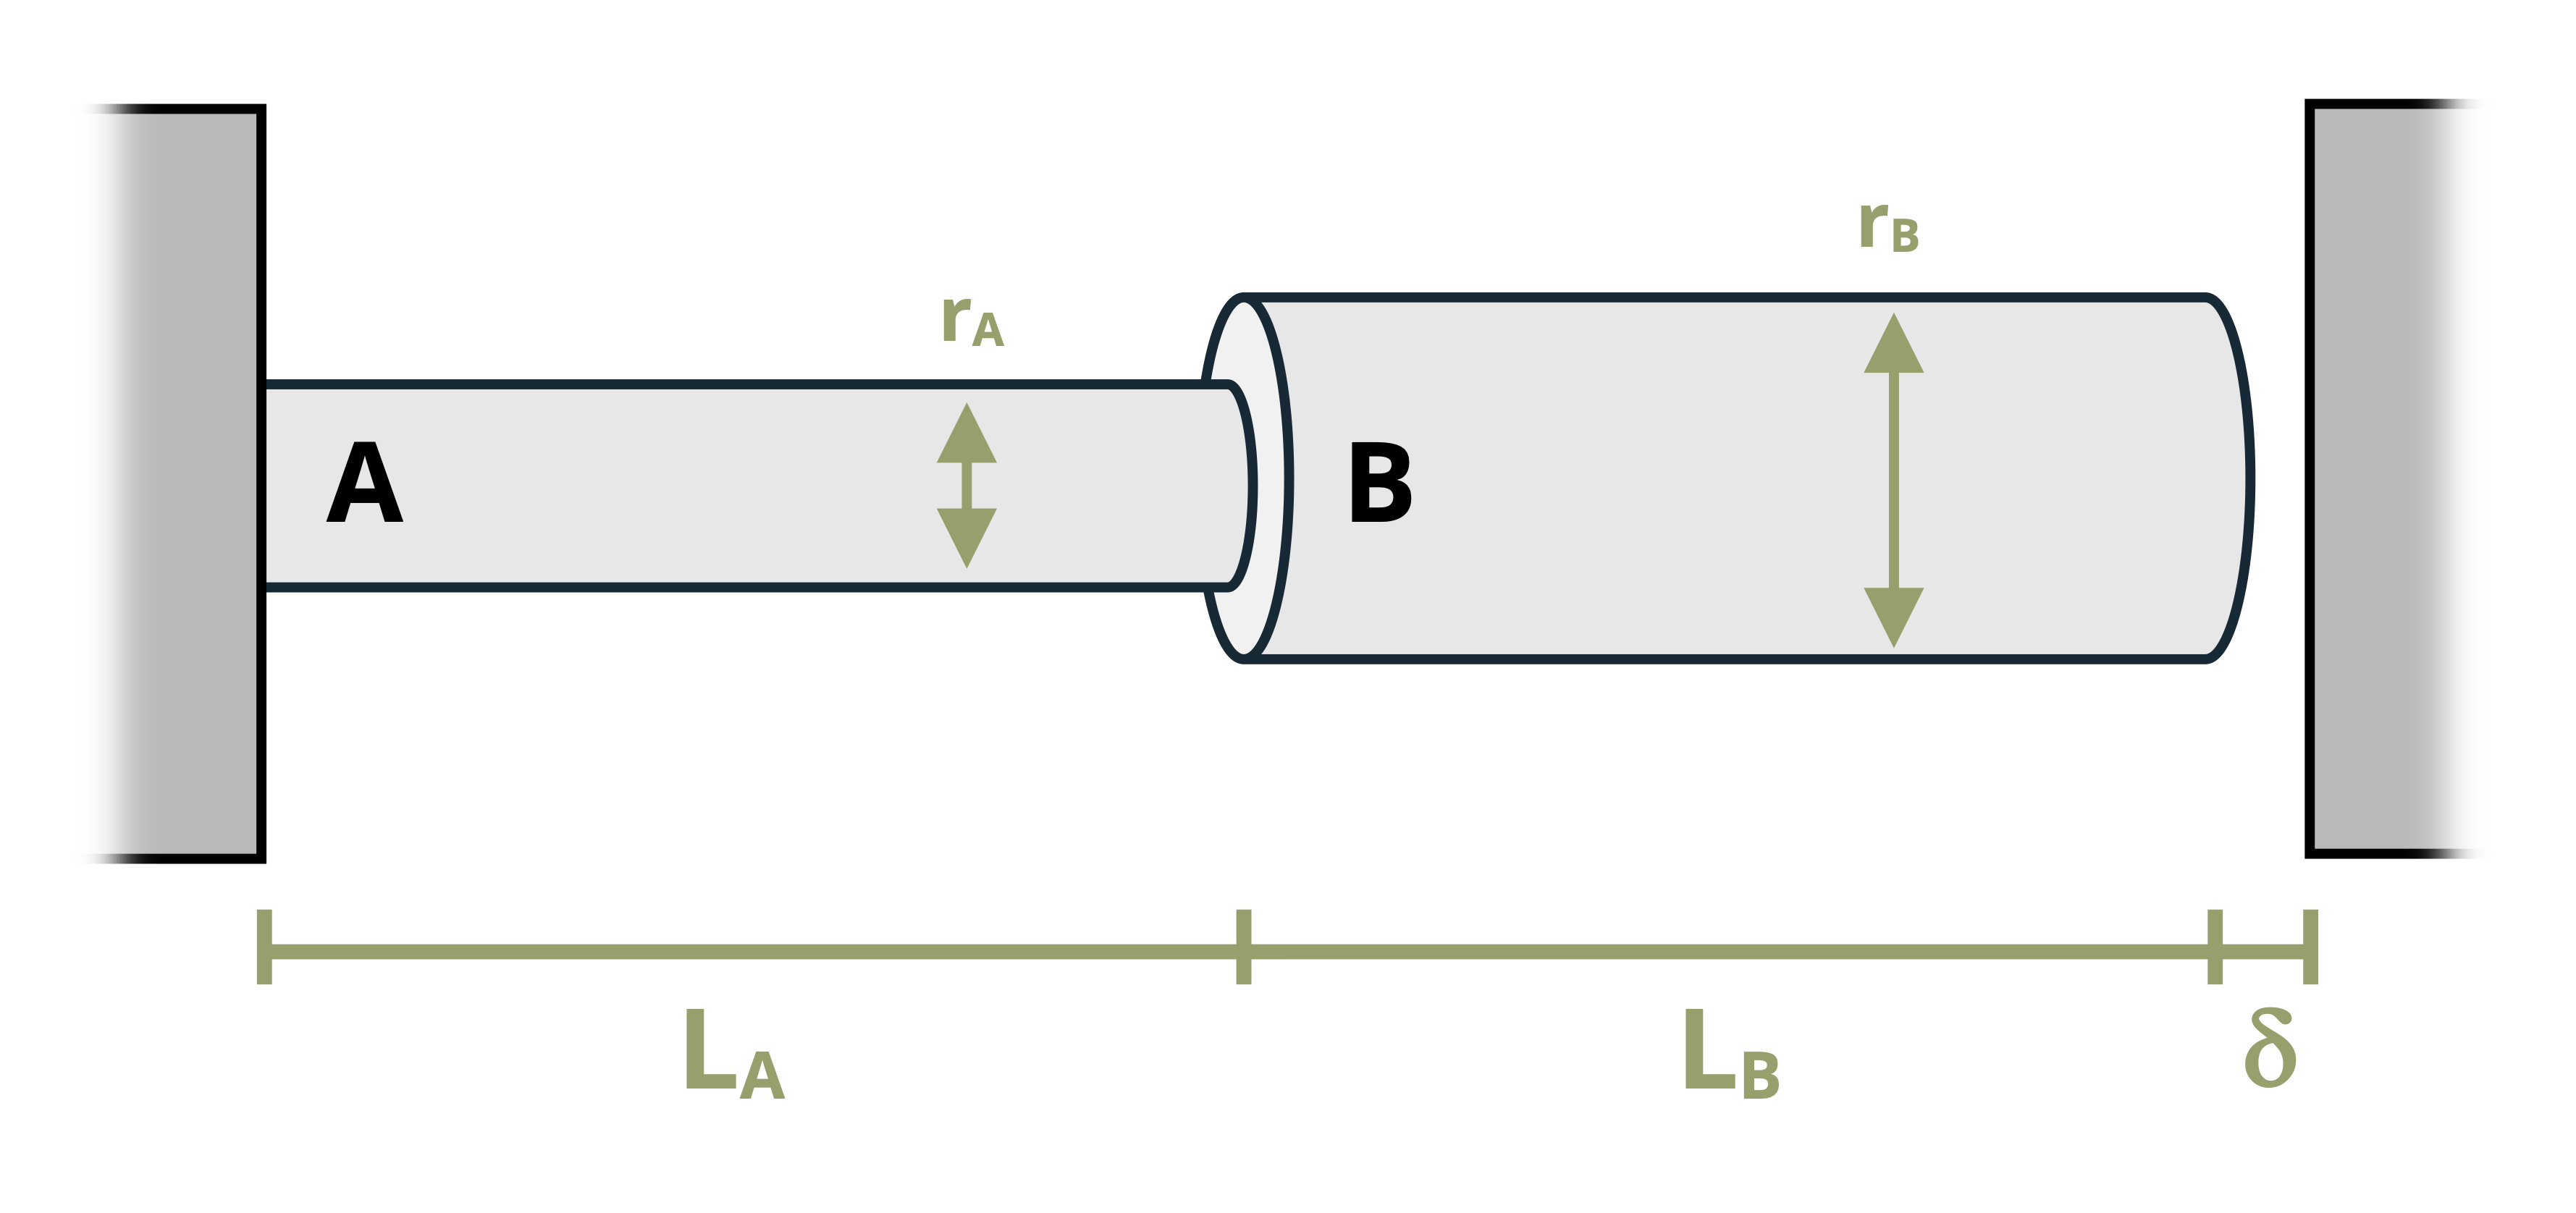
\includegraphics[keepaspectratio]{images/224.png}}
{[}Problem adapted from © Kurt Gramoll CC BY NC-SA 4.0{]}

\begin{Shaded}
\begin{Highlighting}[]
\NormalTok{\#| standalone: true}
\NormalTok{\#| viewerHeight: 600}
\NormalTok{\#| components: [viewer]}

\NormalTok{from shiny import App, render, ui, reactive}
\NormalTok{import random}
\NormalTok{import asyncio}
\NormalTok{import io}
\NormalTok{import math}
\NormalTok{import string}
\NormalTok{from datetime import datetime}
\NormalTok{from pathlib import Path}

\NormalTok{def generate\_random\_letters(length):}
\NormalTok{    \# Generate a random string of letters of specified length}
\NormalTok{    return \textquotesingle{}\textquotesingle{}.join(random.choice(string.ascii\_lowercase) for \_ in range(length)) }

\NormalTok{problem\_ID="224"}
\NormalTok{d=reactive.Value("\_\_")}
\NormalTok{rA=reactive.Value("\_\_")}
\NormalTok{rB=reactive.Value("\_\_")}
\NormalTok{L1=reactive.Value("\_\_")}
\NormalTok{L2=reactive.Value("\_\_")}
\NormalTok{alphaA=6*10**{-}6}
\NormalTok{alphaB=10*10**{-}6}

\NormalTok{attempts=["Timestamp,Attempt,Answer,Feedback\textbackslash{}n"]}

\NormalTok{app\_ui = ui.page\_fluid(}
\NormalTok{    ui.markdown("**Please enter your ID number from your instructor and click to generate your problem**"),}
\NormalTok{    ui.input\_text("ID","", placeholder="Enter ID Number Here"),}
\NormalTok{    ui.input\_action\_button("generate\_problem", "Generate Problem", class\_="btn{-}primary"),}
\NormalTok{    ui.markdown("**Problem Statement**"),}
\NormalTok{    ui.output\_ui("ui\_problem\_statement"),}
\NormalTok{    ui.input\_text("answer","Your Answer in units of °F", placeholder="Please enter your answer"),}
\NormalTok{    ui.input\_action\_button("submit", "Submit Answer", class\_="btn{-}primary"),}
\NormalTok{    ui.download\_button("download", "Download File to Submit", class\_="btn{-}success"),}
\NormalTok{)}


\NormalTok{def server(input, output, session):}
\NormalTok{    \# Initialize a counter for attempts}
\NormalTok{    attempt\_counter = reactive.Value(0)}

\NormalTok{    @output}
\NormalTok{    @render.ui}
\NormalTok{    def ui\_problem\_statement():}
\NormalTok{        return[ui.markdown(f"Two cylindrical rods are heated until they expand, just closing the gap of d = \{d()\} in. The coefficient of thermal expansion, α, for material A and B is 6 x 10\textless{}sup\textgreater{}{-}6\textless{}/sup\textgreater{}/°F and 10 x 10\textless{}sup\textgreater{}{-}6\textless{}/sup\textgreater{}/°F, respectively. The radius of A r\textless{}sub\textgreater{}A\textless{}/sub\textgreater{} = \{rA()\} in and the length is L\textless{}sub\textgreater{}1\textless{}/sub\textgreater{} = \{L1()\} in. The radius of B is r\textless{}sub\textgreater{}B\textless{}/sub\textgreater{} = \{rB()\} in and the length is L\textless{}sub\textgreater{}2\textless{}/sub\textgreater{} = \{L2()\} in. What is the change in temperature.  ")]}
    
\NormalTok{    @reactive.Effect}
\NormalTok{    @reactive.event(input.generate\_problem)}
\NormalTok{    def randomize\_vars():}
\NormalTok{        random.seed(input.ID())}
\NormalTok{        d.set(random.randrange(1, 20, 1)/100)}
\NormalTok{        rA.set(random.randrange(5, 20, 1)/10)}
\NormalTok{        rB.set(round(rA()*1.6, 2))}
\NormalTok{        L1.set(random.randrange(5, 20, 1))}
\NormalTok{        L2.set(round(L1()*0.6, 2))}
        
        
\NormalTok{    @reactive.Effect}
\NormalTok{    @reactive.event(input.submit)}
\NormalTok{    def \_():}
\NormalTok{        attempt\_counter.set(attempt\_counter() + 1)  \# Increment the attempt counter on each submission.}
\NormalTok{        instr= d()/(alphaA*L1()+alphaB*L2())}
\NormalTok{        if math.isclose(float(input.answer()), instr, rel\_tol=0.01):}
\NormalTok{            check = "*Correct*"}
\NormalTok{            correct\_indicator = "JL"}
\NormalTok{        else:}
\NormalTok{            check = "*Not Correct.*"}
\NormalTok{            correct\_indicator = "JG"}

\NormalTok{        \# Generate random parts for the encoded attempt.}
\NormalTok{        random\_start = generate\_random\_letters(4)}
\NormalTok{        random\_middle = generate\_random\_letters(4)}
\NormalTok{        random\_end = generate\_random\_letters(4)}
\NormalTok{        encoded\_attempt = f"\{random\_start\}\{problem\_ID\}{-}\{random\_middle\}\{attempt\_counter()\}\{correct\_indicator\}{-}\{random\_end\}\{input.ID()\}"}

\NormalTok{        \# Store the most recent encoded attempt in a reactive value so it persists across submissions}
\NormalTok{        session.encoded\_attempt = reactive.Value(encoded\_attempt)}

\NormalTok{        \# Append the attempt data to the attempts list without the encoded attempt}
\NormalTok{        attempts.append(f"\{datetime.now()\}, \{attempt\_counter()\}, \{input.answer()\}, \{check\}\textbackslash{}n")}

\NormalTok{        \# Show feedback to the user.}
\NormalTok{        feedback = ui.markdown(f"Your answer of \{input.answer()\} is \{check\}.")}
\NormalTok{        m = ui.modal(}
\NormalTok{            feedback,}
\NormalTok{            title="Feedback",}
\NormalTok{            easy\_close=True}
\NormalTok{        )}
\NormalTok{        ui.modal\_show(m)}

\NormalTok{    @session.download(filename=lambda: f"Problem\_Log{-}\{problem\_ID\}{-}\{input.ID()\}.csv")}
\NormalTok{    async def download():}
\NormalTok{        \# Start the CSV with the encoded attempt (without label)}
\NormalTok{        final\_encoded = session.encoded\_attempt() if session.encoded\_attempt is not None else "No attempts"}
\NormalTok{        yield f"\{final\_encoded\}\textbackslash{}n\textbackslash{}n"}
        
\NormalTok{        \# Write the header for the remaining CSV data once}
\NormalTok{        yield "Timestamp,Attempt,Answer,Feedback\textbackslash{}n"}
        
\NormalTok{        \# Write the attempts data, ensure that the header from the attempts list is not written again}
\NormalTok{        for attempt in attempts[1:]:  \# Skip the first element which is the header}
\NormalTok{            await asyncio.sleep(0.25)  \# This delay may not be necessary; adjust as needed}
\NormalTok{            yield attempt}


\NormalTok{\# App installation}
\NormalTok{app = App(app\_ui, server)}
\end{Highlighting}
\end{Shaded}

\chapter*{Problem 5.53 - Thermal
Deformation}\label{problem-5.53---thermal-deformation}
\addcontentsline{toc}{chapter}{Problem 5.53 - Thermal Deformation}

\markboth{Problem 5.53 - Thermal Deformation}{Problem 5.53 - Thermal
Deformation}

\pandocbounded{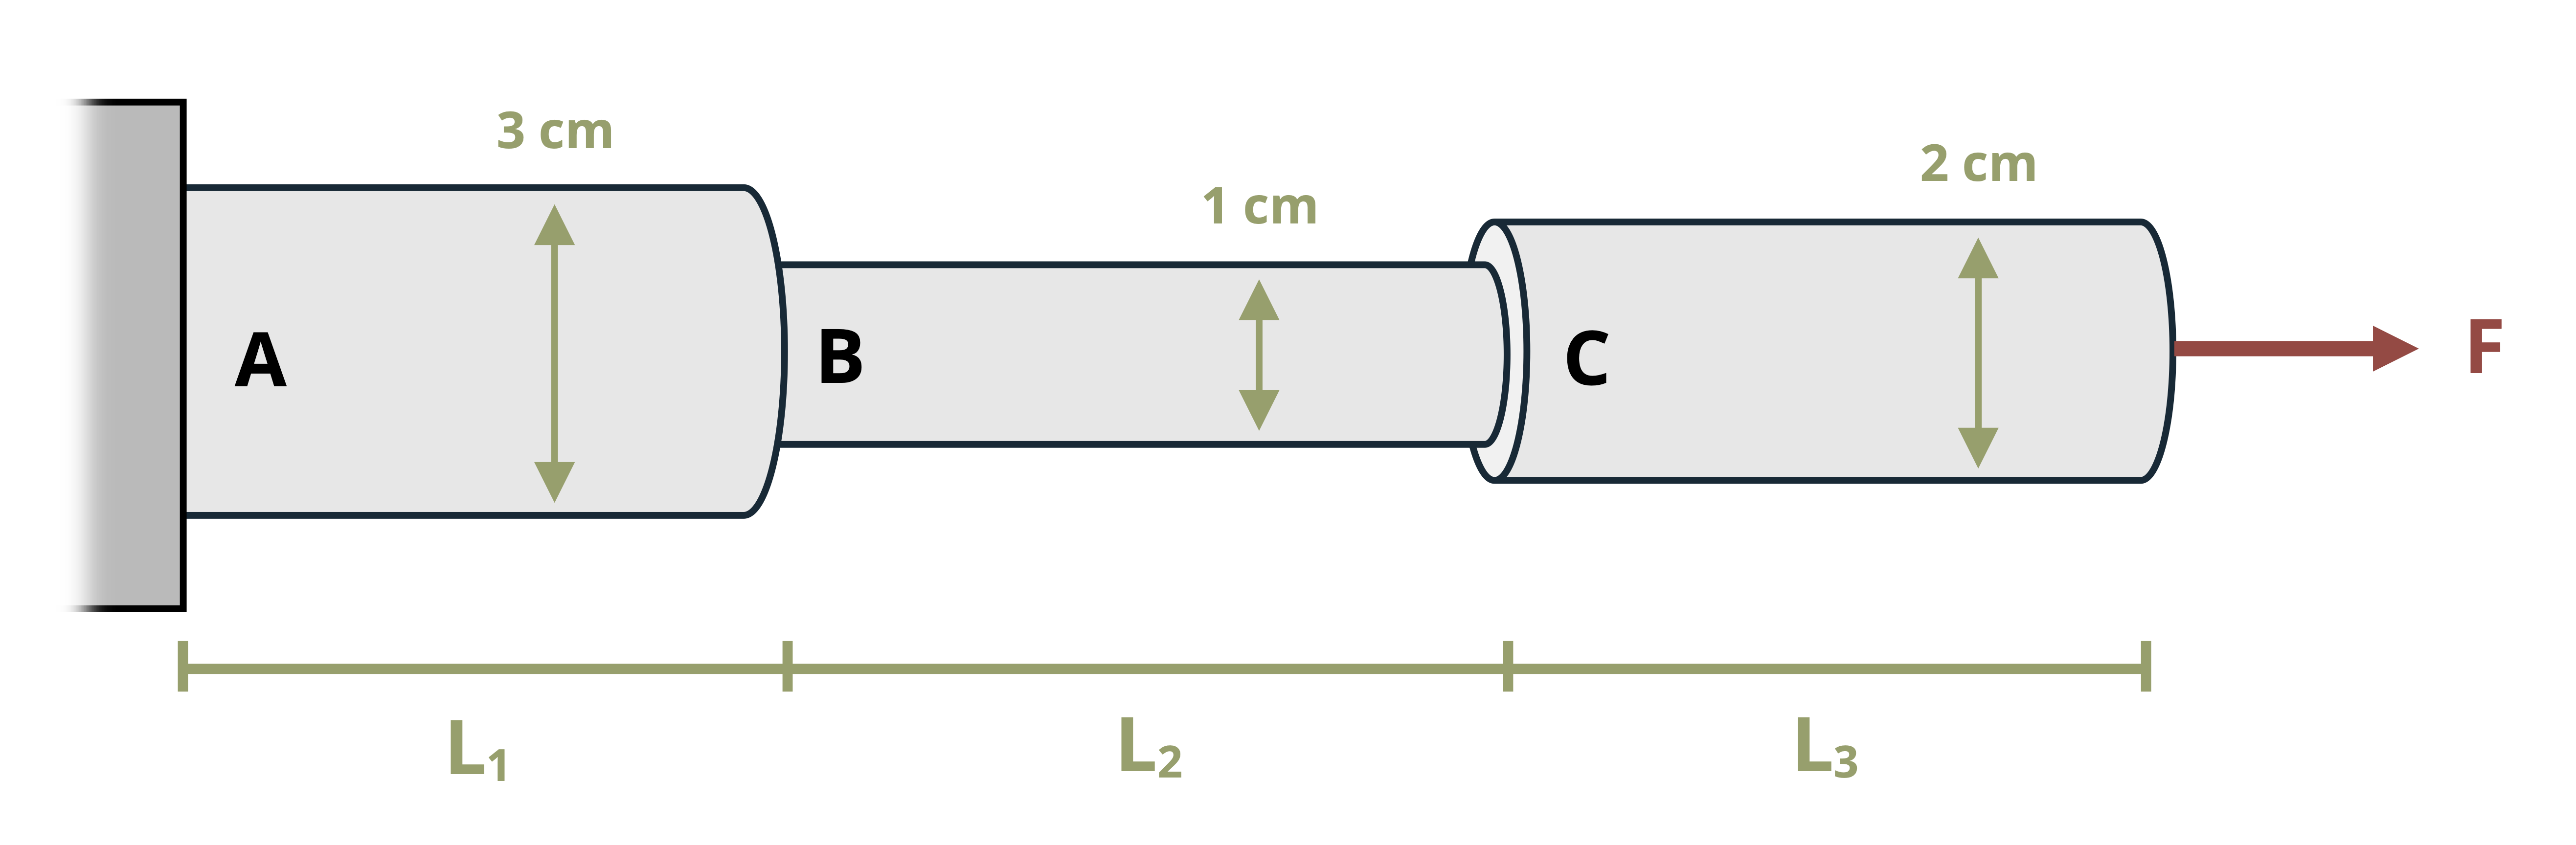
\includegraphics[keepaspectratio]{images/225.png}}
{[}Problem adapted from © Kurt Gramoll CC BY NC-SA 4.0{]}

\begin{Shaded}
\begin{Highlighting}[]
\NormalTok{\#| standalone: true}
\NormalTok{\#| viewerHeight: 600}
\NormalTok{\#| components: [viewer]}

\NormalTok{from shiny import App, render, ui, reactive}
\NormalTok{import random}
\NormalTok{import asyncio}
\NormalTok{import io}
\NormalTok{import math}
\NormalTok{import string}
\NormalTok{from datetime import datetime}
\NormalTok{from pathlib import Path}

\NormalTok{def generate\_random\_letters(length):}
\NormalTok{    \# Generate a random string of letters of specified length}
\NormalTok{    return \textquotesingle{}\textquotesingle{}.join(random.choice(string.ascii\_lowercase) for \_ in range(length)) }

\NormalTok{problem\_ID="225"}
\NormalTok{L1=reactive.Value("\_\_")}
\NormalTok{L2=reactive.Value("\_\_")}
\NormalTok{L3=reactive.Value("\_\_")}
\NormalTok{F=reactive.Value("\_\_")}
\NormalTok{dT=reactive.Value("\_\_")}
\NormalTok{alphaA=10*10**{-}6}
\NormalTok{alphaB=5*10**{-}6}
\NormalTok{alphaC=7*10**{-}6}
\NormalTok{EA=40*10**9}
\NormalTok{EB=120*10**9}
\NormalTok{EC=80*10**9}

\NormalTok{attempts=["Timestamp,Attempt,Answer,Feedback\textbackslash{}n"]}

\NormalTok{app\_ui = ui.page\_fluid(}
\NormalTok{    ui.markdown("**Please enter your ID number from your instructor and click to generate your problem**"),}
\NormalTok{    ui.input\_text("ID","", placeholder="Enter ID Number Here"),}
\NormalTok{    ui.input\_action\_button("generate\_problem", "Generate Problem", class\_="btn{-}primary"),}
\NormalTok{    ui.markdown("**Problem Statement**"),}
\NormalTok{    ui.output\_ui("ui\_problem\_statement"),}
\NormalTok{    ui.input\_text("answer","Your Answer in units of mm", placeholder="Please enter your answer"),}
\NormalTok{    ui.input\_action\_button("submit", "Submit Answer", class\_="btn{-}primary"),}
\NormalTok{    ui.download\_button("download", "Download File to Submit", class\_="btn{-}success"),}
\NormalTok{)}


\NormalTok{def server(input, output, session):}
\NormalTok{    \# Initialize a counter for attempts}
\NormalTok{    attempt\_counter = reactive.Value(0)}

\NormalTok{    @output}
\NormalTok{    @render.ui}
\NormalTok{    def ui\_problem\_statement():}
\NormalTok{        return[ui.markdown(f"Three cylindrical rods of lengths L\textless{}sub\textgreater{}1\textless{}/sub\textgreater{} = \{L1()\} m, L\textless{}sub\textgreater{}2\textless{}/sub\textgreater{} = \{L2()\} m, and L\textless{}sub\textgreater{}3\textless{}/sub\textgreater{} = \{L3()\} m are connected together. A force F = \{F()\} kN is applied to the free end and all three rods are heated by \{dT()\} °C. The coefficient of thermal expansion, α, and elastic modulus, E, for each material are α\textless{}sub\textgreater{}A\textless{}/sub\textgreater{} = 10 x 10\textless{}sup\textgreater{}{-}6\textless{}/sup\textgreater{} /°C, α\textless{}sub\textgreater{}B\textless{}/sub\textgreater{} = 5 x 10\textless{}sup\textgreater{}{-}6\textless{}/sup\textgreater{} /°C, α\textless{}sub\textgreater{}C\textless{}/sub\textgreater{} = 7 x 10\textless{}sup\textgreater{}{-}6\textless{}/sup\textgreater{} /°C, E\textless{}sub\textgreater{}A\textless{}/sub\textgreater{} = 40 GPa, E\textless{}sub\textgreater{}B\textless{}/sub\textgreater{} = 120 GPa, and E\textless{}sub\textgreater{}C\textless{}/sub\textgreater{} = 80 GPa. What is the total deflection of the right rod tip?  ")]}
    
\NormalTok{    @reactive.Effect}
\NormalTok{    @reactive.event(input.generate\_problem)}
\NormalTok{    def randomize\_vars():}
\NormalTok{        random.seed(input.ID())}
\NormalTok{        L1.set(random.randrange(10, 40, 1)/10)}
\NormalTok{        L2.set(round((L1()*0.8),1))}
\NormalTok{        L3.set(round((L1()*2/3),1))        }
\NormalTok{        F.set(random.randrange(5, 50, 1))}
\NormalTok{        dT.set(random.randrange(100, 300, 10))}
        
\NormalTok{    @reactive.Effect}
\NormalTok{    @reactive.event(input.submit)}
\NormalTok{    def \_():}
\NormalTok{        attempt\_counter.set(attempt\_counter() + 1)  \# Increment the attempt counter on each submission.}
\NormalTok{        deltaL = (F()*L1()*1000)/(EA*math.pi*.015**2) + (F()*L2()*1000)/(EB*math.pi*.005**2) + (F()*L3()*1000)/(EC*math.pi*.01**2)}
\NormalTok{        deltaT = alphaA*dT()*L1() + alphaB*dT()*L2() + alphaC*dT()*L3() }
\NormalTok{        instr= (deltaL + deltaT)*1000}
\NormalTok{        if math.isclose(float(input.answer()), instr, rel\_tol=0.01):}
\NormalTok{            check = "*Correct*"}
\NormalTok{            correct\_indicator = "JL"}
\NormalTok{        else:}
\NormalTok{            check = "*Not Correct.*"}
\NormalTok{            correct\_indicator = "JG"}

\NormalTok{        \# Generate random parts for the encoded attempt.}
\NormalTok{        random\_start = generate\_random\_letters(4)}
\NormalTok{        random\_middle = generate\_random\_letters(4)}
\NormalTok{        random\_end = generate\_random\_letters(4)}
\NormalTok{        encoded\_attempt = f"\{random\_start\}\{problem\_ID\}{-}\{random\_middle\}\{attempt\_counter()\}\{correct\_indicator\}{-}\{random\_end\}\{input.ID()\}"}

\NormalTok{        \# Store the most recent encoded attempt in a reactive value so it persists across submissions}
\NormalTok{        session.encoded\_attempt = reactive.Value(encoded\_attempt)}

\NormalTok{        \# Append the attempt data to the attempts list without the encoded attempt}
\NormalTok{        attempts.append(f"\{datetime.now()\}, \{attempt\_counter()\}, \{input.answer()\}, \{check\}\textbackslash{}n")}

\NormalTok{        \# Show feedback to the user.}
\NormalTok{        feedback = ui.markdown(f"Your answer of \{input.answer()\} is \{check\}.")}
\NormalTok{        m = ui.modal(}
\NormalTok{            feedback,}
\NormalTok{            title="Feedback",}
\NormalTok{            easy\_close=True}
\NormalTok{        )}
\NormalTok{        ui.modal\_show(m)}

\NormalTok{    @session.download(filename=lambda: f"Problem\_Log{-}\{problem\_ID\}{-}\{input.ID()\}.csv")}
\NormalTok{    async def download():}
\NormalTok{        \# Start the CSV with the encoded attempt (without label)}
\NormalTok{        final\_encoded = session.encoded\_attempt() if session.encoded\_attempt is not None else "No attempts"}
\NormalTok{        yield f"\{final\_encoded\}\textbackslash{}n\textbackslash{}n"}
        
\NormalTok{        \# Write the header for the remaining CSV data once}
\NormalTok{        yield "Timestamp,Attempt,Answer,Feedback\textbackslash{}n"}
        
\NormalTok{        \# Write the attempts data, ensure that the header from the attempts list is not written again}
\NormalTok{        for attempt in attempts[1:]:  \# Skip the first element which is the header}
\NormalTok{            await asyncio.sleep(0.25)  \# This delay may not be necessary; adjust as needed}
\NormalTok{            yield attempt}

\NormalTok{\# App installation}
\NormalTok{app = App(app\_ui, server)}
\end{Highlighting}
\end{Shaded}

\chapter*{Problem 5.54 - Thermal
Deformation}\label{problem-5.54---thermal-deformation}
\addcontentsline{toc}{chapter}{Problem 5.54 - Thermal Deformation}

\markboth{Problem 5.54 - Thermal Deformation}{Problem 5.54 - Thermal
Deformation}

\pandocbounded{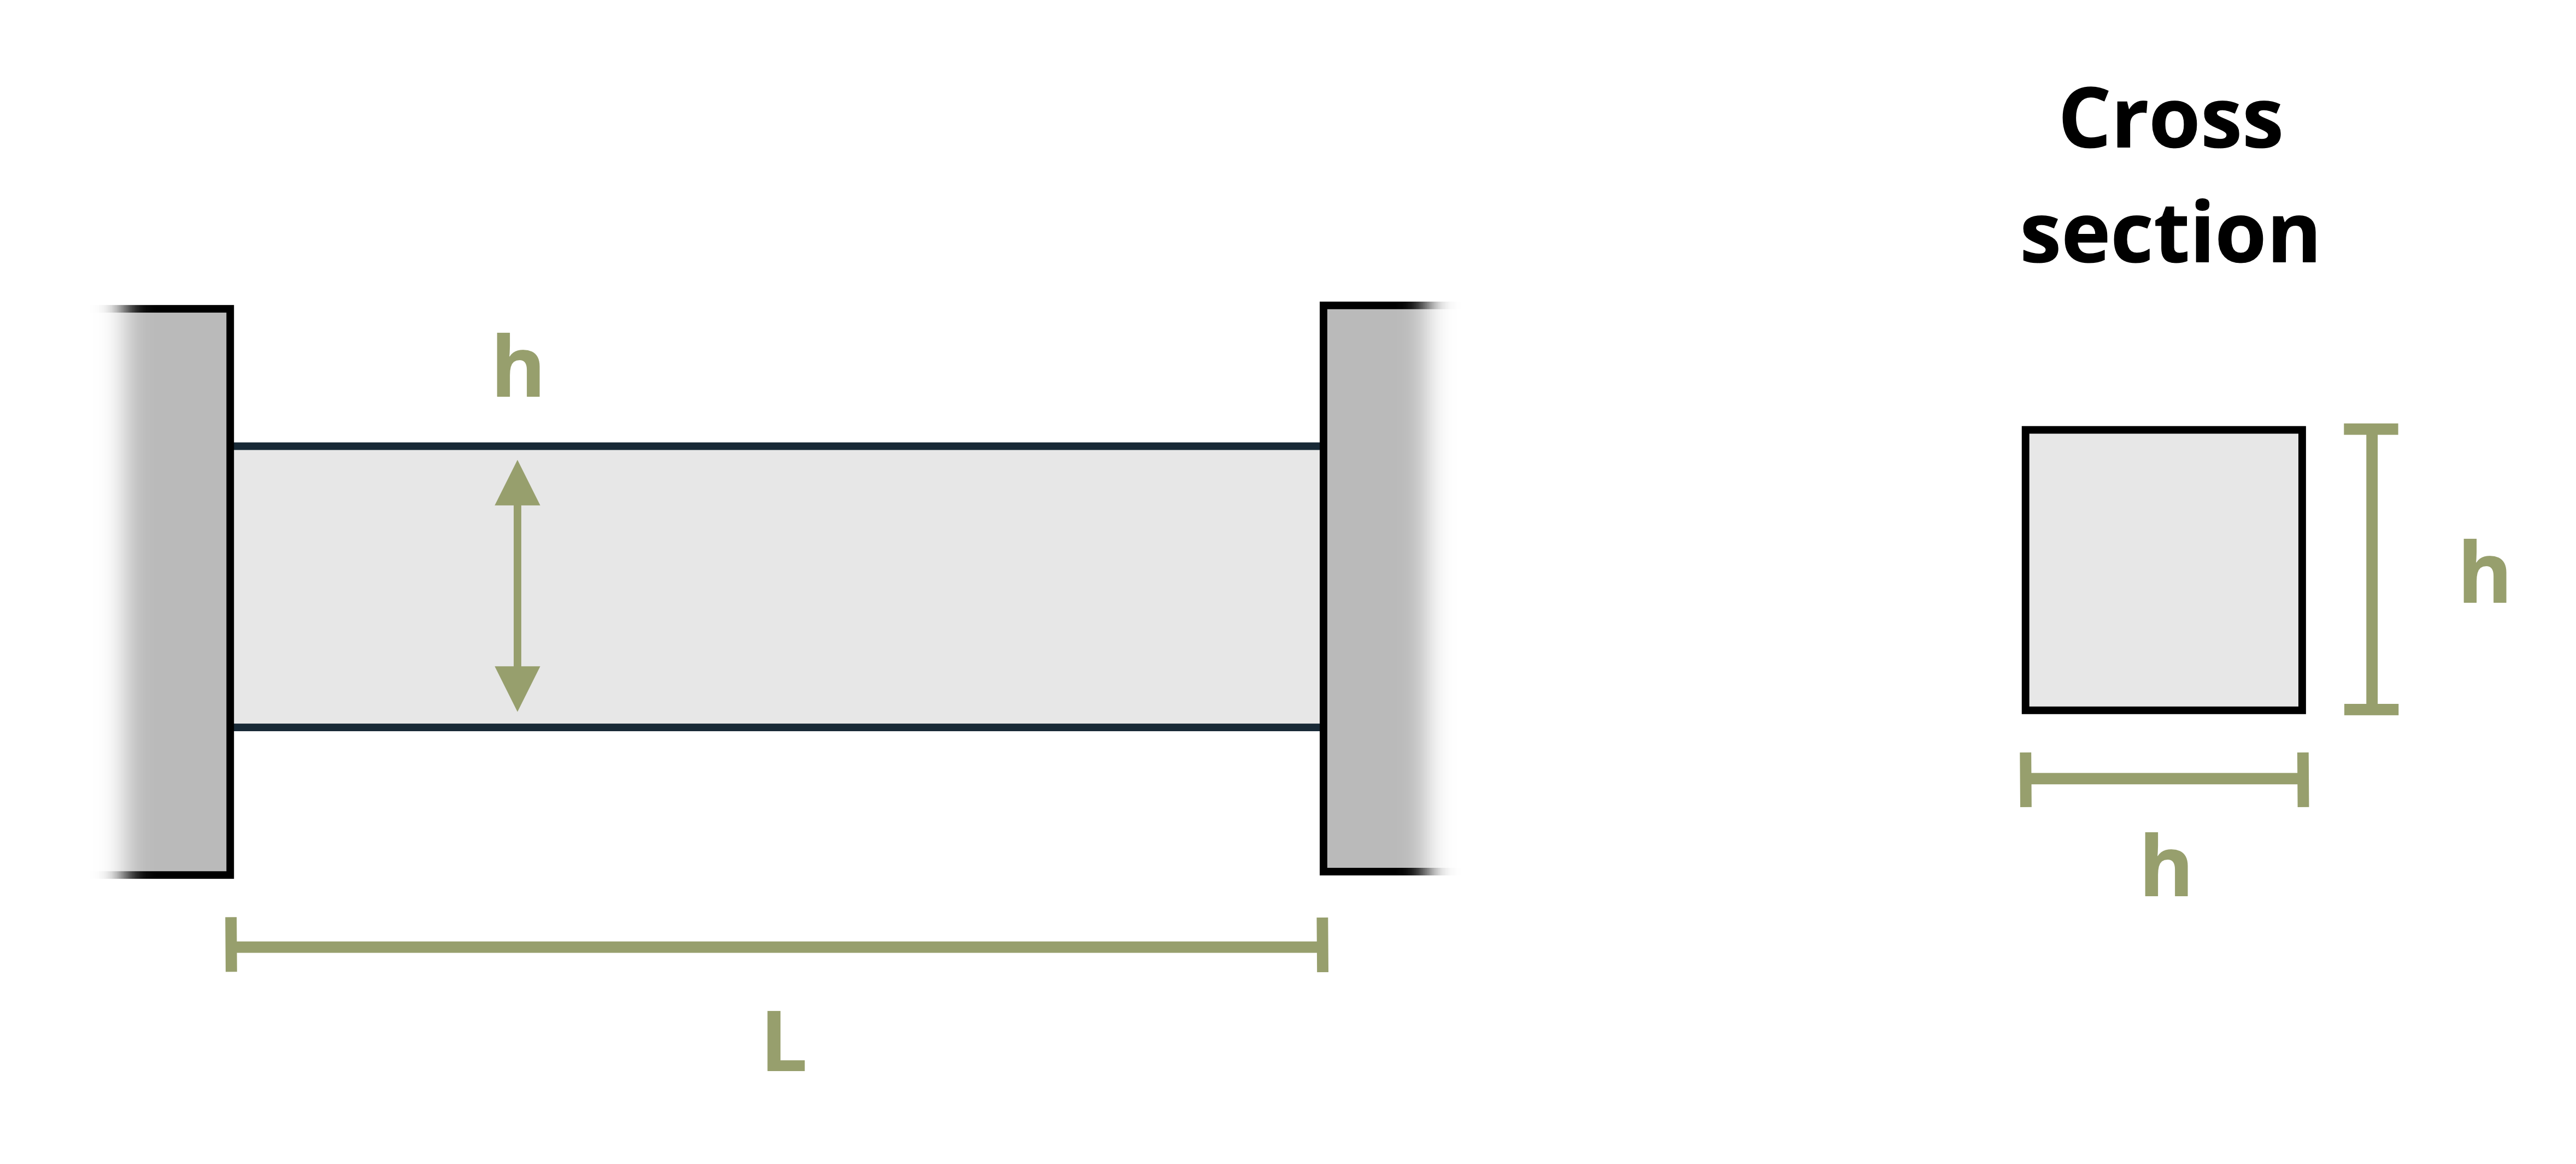
\includegraphics[keepaspectratio]{images/226.png}}
{[}Problem adapted from © Kurt Gramoll CC BY NC-SA 4.0{]}

\begin{Shaded}
\begin{Highlighting}[]
\NormalTok{\#| standalone: true}
\NormalTok{\#| viewerHeight: 600}
\NormalTok{\#| components: [viewer]}

\NormalTok{from shiny import App, render, ui, reactive}
\NormalTok{import random}
\NormalTok{import asyncio}
\NormalTok{import io}
\NormalTok{import math}
\NormalTok{import string}
\NormalTok{from datetime import datetime}
\NormalTok{from pathlib import Path}

\NormalTok{def generate\_random\_letters(length):}
\NormalTok{    \# Generate a random string of letters of specified length}
\NormalTok{    return \textquotesingle{}\textquotesingle{}.join(random.choice(string.ascii\_lowercase) for \_ in range(length)) }

\NormalTok{problem\_ID="226"}
\NormalTok{T1=reactive.Value("\_\_")}
\NormalTok{T2=reactive.Value("\_\_")}
\NormalTok{L=reactive.Value("\_\_")}
\NormalTok{h=reactive.Value("\_\_")}
\NormalTok{alpha=20*10**{-}6}
\NormalTok{E=100*10**9}

\NormalTok{attempts=["Timestamp,Attempt,Answer,Feedback\textbackslash{}n"]}

\NormalTok{app\_ui = ui.page\_fluid(}
\NormalTok{    ui.markdown("**Please enter your ID number from your instructor and click to generate your problem**"),}
\NormalTok{    ui.input\_text("ID","", placeholder="Enter ID Number Here"),}
\NormalTok{    ui.input\_action\_button("generate\_problem", "Generate Problem", class\_="btn{-}primary"),}
\NormalTok{    ui.markdown("**Problem Statement**"),}
\NormalTok{    ui.output\_ui("ui\_problem\_statement"),}
\NormalTok{    ui.input\_text("answer","Your Answer in units of MPa", placeholder="Please enter your answer"),}
\NormalTok{    ui.input\_action\_button("submit", "Submit Answer", class\_="btn{-}primary"),}
\NormalTok{    ui.download\_button("download", "Download File to Submit", class\_="btn{-}success"),}
\NormalTok{)}


\NormalTok{def server(input, output, session):}
\NormalTok{    \# Initialize a counter for attempts}
\NormalTok{    attempt\_counter = reactive.Value(0)}

\NormalTok{    @output}
\NormalTok{    @render.ui}
\NormalTok{    def ui\_problem\_statement():}
\NormalTok{        return[ui.markdown(f"A square brass bar is placed between two fixed walls and heated from \{T1()\}°C to \{T2()\}°C. If L = \{L()\} mm, h = \{h()\} mm, E = 100 GPa, and α = 20 x 10\textless{}sup\textgreater{}{-}6\textless{}/sup\textgreater{} /°C, determine the stress in the bar.  ")]}
    
\NormalTok{    @reactive.Effect}
\NormalTok{    @reactive.event(input.generate\_problem)}
\NormalTok{    def randomize\_vars():}
\NormalTok{        random.seed(input.ID())}
\NormalTok{        T1.set(random.randrange(5, 20, 1))}
\NormalTok{        T2.set(round(T1() + random.randrange(20, 50, 1), 2))}
\NormalTok{        L.set(random.randrange(250, 750, 10))}
\NormalTok{        h.set(random.randrange(10, 30, 1))}
       
        
\NormalTok{    @reactive.Effect}
\NormalTok{    @reactive.event(input.submit)}
\NormalTok{    def \_():}
\NormalTok{        attempt\_counter.set(attempt\_counter() + 1)  \# Increment the attempt counter on each submission.}
\NormalTok{        instr= (E*alpha*(T2(){-}T1()))/10**6}
\NormalTok{        if math.isclose(float(input.answer()), instr, rel\_tol=0.01):}
\NormalTok{            check = "*Correct*"}
\NormalTok{            correct\_indicator = "JL"}
\NormalTok{        else:}
\NormalTok{            check = "*Not Correct.*"}
\NormalTok{            correct\_indicator = "JG"}

\NormalTok{        \# Generate random parts for the encoded attempt.}
\NormalTok{        random\_start = generate\_random\_letters(4)}
\NormalTok{        random\_middle = generate\_random\_letters(4)}
\NormalTok{        random\_end = generate\_random\_letters(4)}
\NormalTok{        encoded\_attempt = f"\{random\_start\}\{problem\_ID\}{-}\{random\_middle\}\{attempt\_counter()\}\{correct\_indicator\}{-}\{random\_end\}\{input.ID()\}"}

\NormalTok{        \# Store the most recent encoded attempt in a reactive value so it persists across submissions}
\NormalTok{        session.encoded\_attempt = reactive.Value(encoded\_attempt)}

\NormalTok{        \# Append the attempt data to the attempts list without the encoded attempt}
\NormalTok{        attempts.append(f"\{datetime.now()\}, \{attempt\_counter()\}, \{input.answer()\}, \{check\}\textbackslash{}n")}

\NormalTok{        \# Show feedback to the user.}
\NormalTok{        feedback = ui.markdown(f"Your answer of \{input.answer()\} is \{check\}.")}
\NormalTok{        m = ui.modal(}
\NormalTok{            feedback,}
\NormalTok{            title="Feedback",}
\NormalTok{            easy\_close=True}
\NormalTok{        )}
\NormalTok{        ui.modal\_show(m)}

\NormalTok{    @session.download(filename=lambda: f"Problem\_Log{-}\{problem\_ID\}{-}\{input.ID()\}.csv")}
\NormalTok{    async def download():}
\NormalTok{        \# Start the CSV with the encoded attempt (without label)}
\NormalTok{        final\_encoded = session.encoded\_attempt() if session.encoded\_attempt is not None else "No attempts"}
\NormalTok{        yield f"\{final\_encoded\}\textbackslash{}n\textbackslash{}n"}
        
\NormalTok{        \# Write the header for the remaining CSV data once}
\NormalTok{        yield "Timestamp,Attempt,Answer,Feedback\textbackslash{}n"}
        
\NormalTok{        \# Write the attempts data, ensure that the header from the attempts list is not written again}
\NormalTok{        for attempt in attempts[1:]:  \# Skip the first element which is the header}
\NormalTok{            await asyncio.sleep(0.25)  \# This delay may not be necessary; adjust as needed}
\NormalTok{            yield attempt}


\NormalTok{\# App installation}
\NormalTok{app = App(app\_ui, server)}
\end{Highlighting}
\end{Shaded}

\chapter*{Problem 5.55 - Thermal
Deformation}\label{problem-5.55---thermal-deformation}
\addcontentsline{toc}{chapter}{Problem 5.55 - Thermal Deformation}

\markboth{Problem 5.55 - Thermal Deformation}{Problem 5.55 - Thermal
Deformation}

\pandocbounded{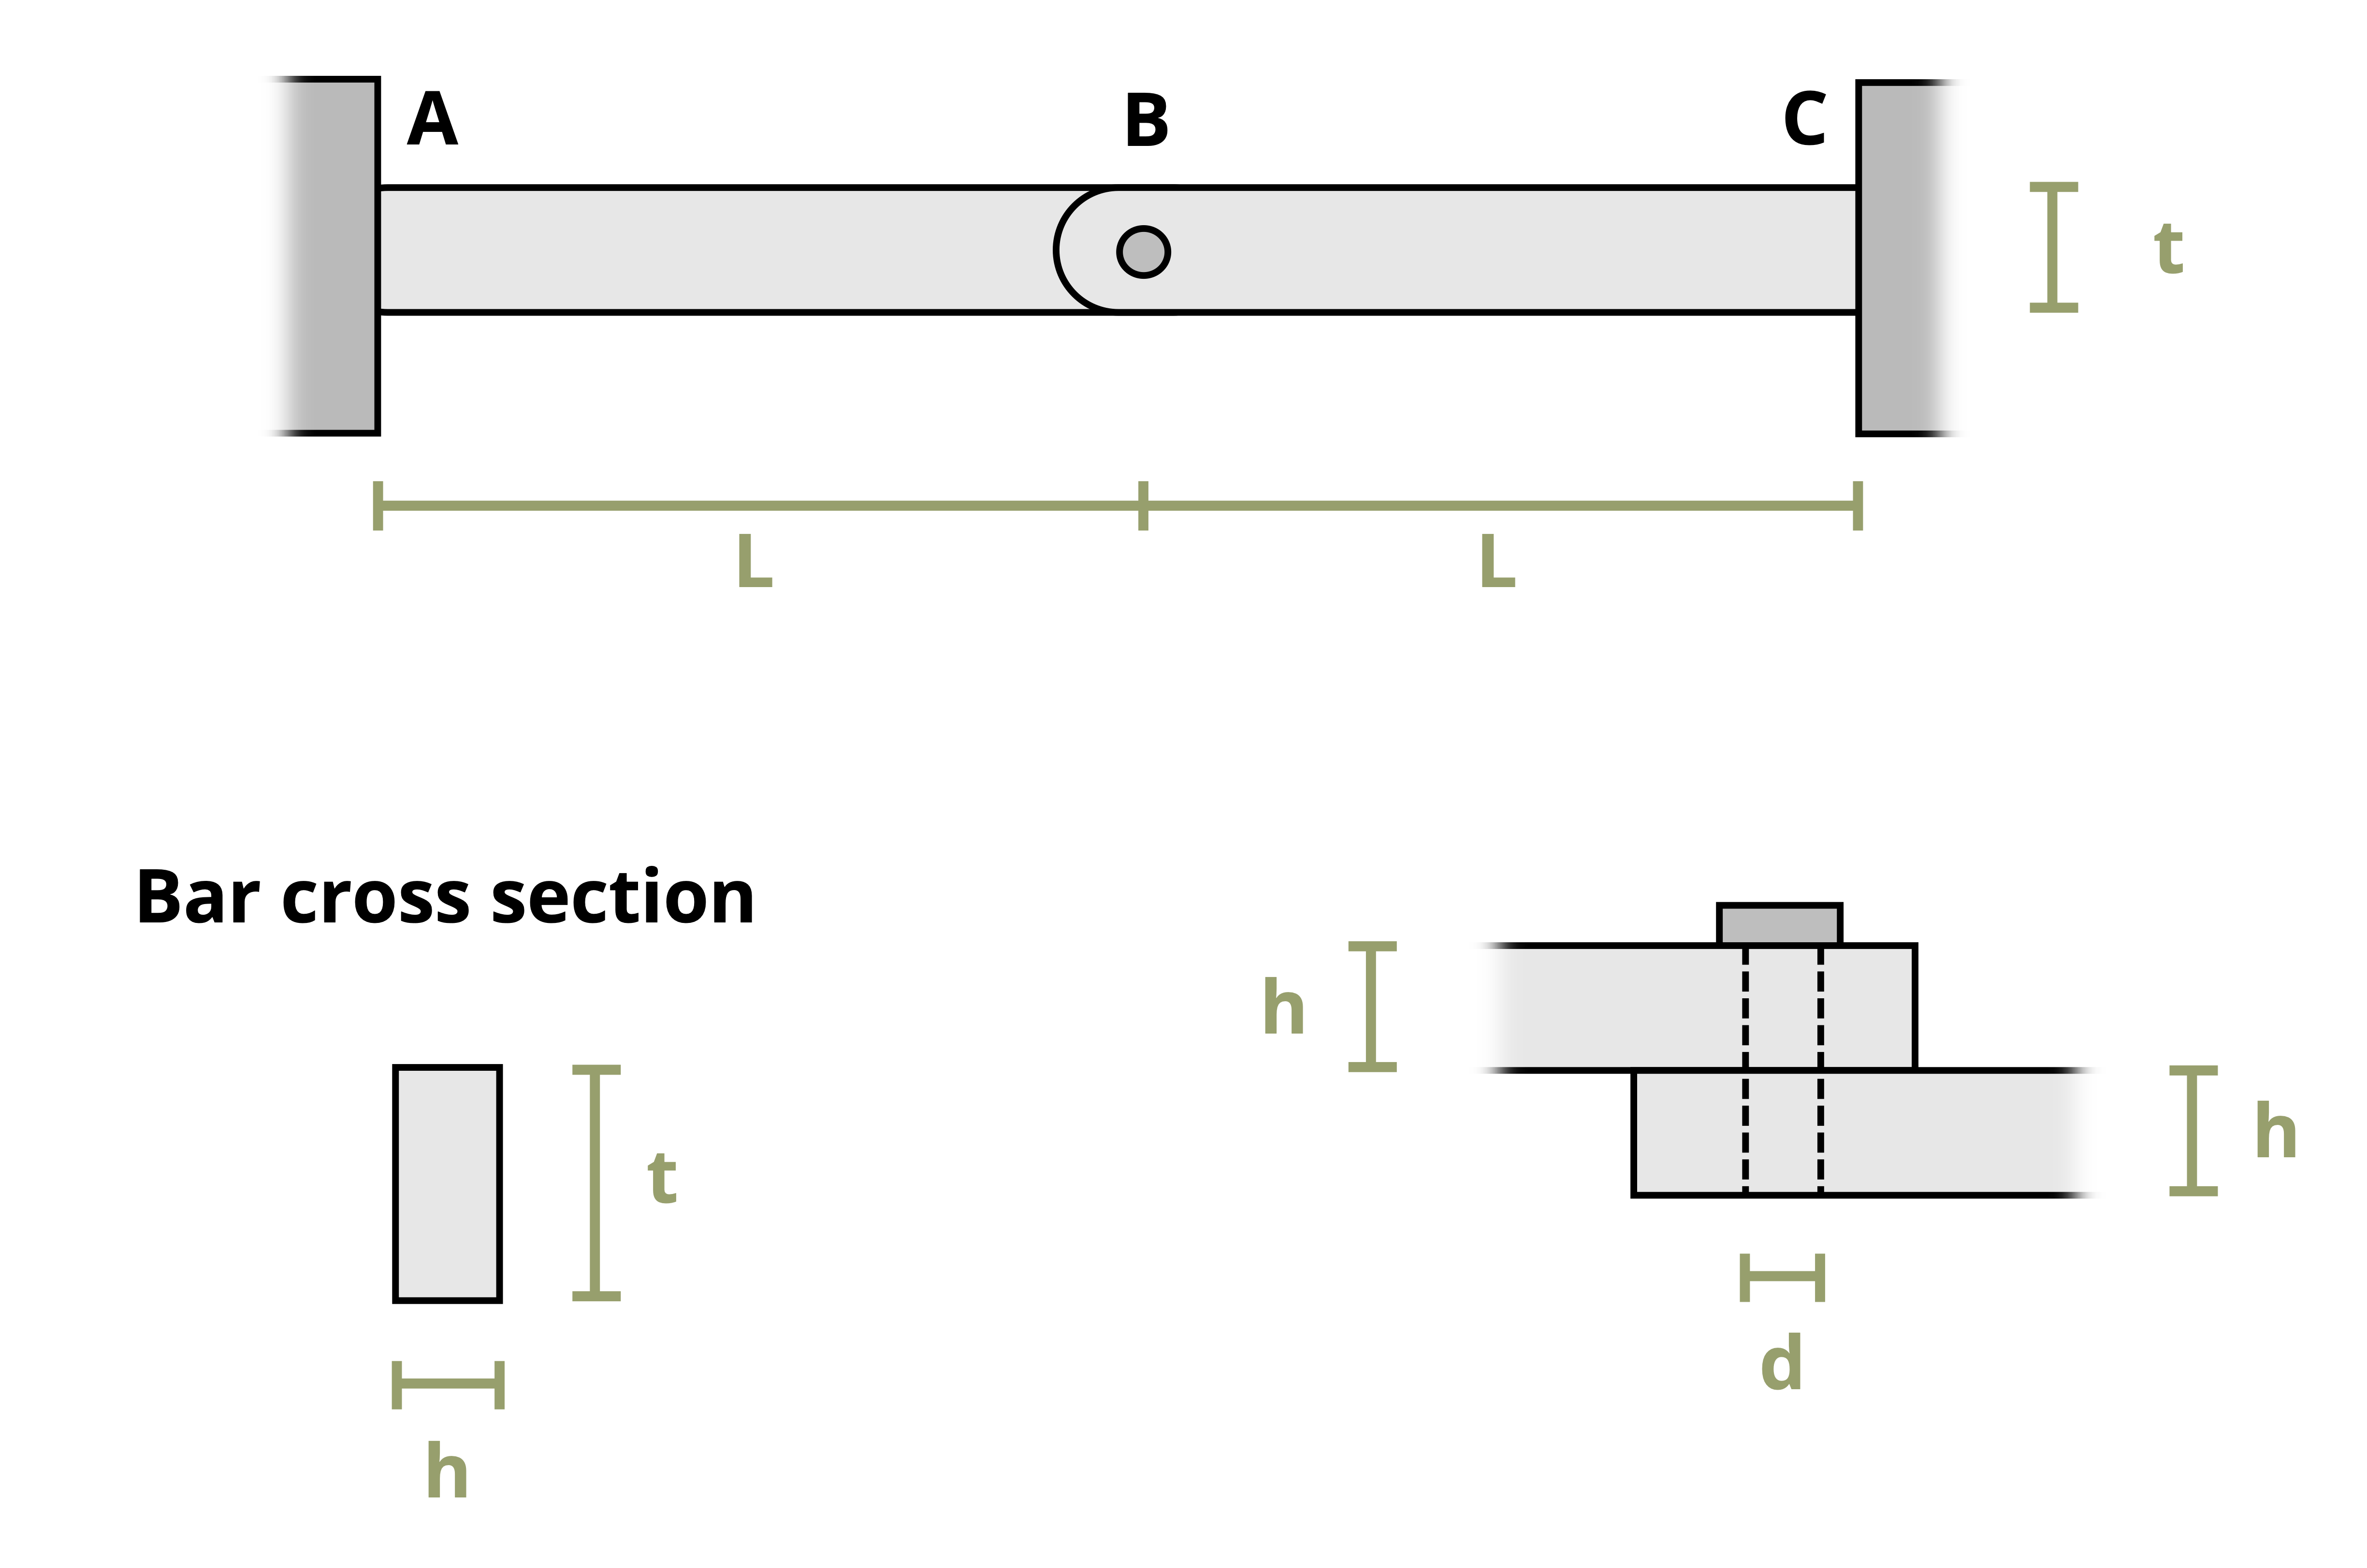
\includegraphics[keepaspectratio]{images/249.png}}
{[}Problem adapted from © Kurt Gramoll CC BY NC-SA 4.0{]}

\begin{Shaded}
\begin{Highlighting}[]
\NormalTok{\#| standalone: true}
\NormalTok{\#| viewerHeight: 600}
\NormalTok{\#| components: [viewer]}

\NormalTok{from shiny import App, render, ui, reactive}
\NormalTok{import random}
\NormalTok{import asyncio}
\NormalTok{import io}
\NormalTok{import math}
\NormalTok{import string}
\NormalTok{from datetime import datetime}
\NormalTok{from pathlib import Path}

\NormalTok{def generate\_random\_letters(length):}
\NormalTok{    \# Generate a random string of letters of specified length}
\NormalTok{    return \textquotesingle{}\textquotesingle{}.join(random.choice(string.ascii\_lowercase) for \_ in range(length)) }

\NormalTok{problem\_ID="249"}
\NormalTok{L=reactive.Value("\_\_")}
\NormalTok{d=reactive.Value("\_\_")}
\NormalTok{t=reactive.Value("\_\_")}
\NormalTok{h=reactive.Value("\_\_")}
\NormalTok{dT=reactive.Value("\_\_")}
\NormalTok{E=200}
\NormalTok{v=0.32}
\NormalTok{a=11.7*10**{-}6}

\NormalTok{attempts=["Timestamp,Attempt,Answer,Feedback\textbackslash{}n"]}

\NormalTok{app\_ui = ui.page\_fluid(}
\NormalTok{    ui.markdown("**Please enter your ID number from your instructor and click to generate your problem**"),}
\NormalTok{    ui.input\_text("ID","", placeholder="Enter ID Number Here"),}
\NormalTok{    ui.input\_action\_button("generate\_problem", "Generate Problem", class\_="btn{-}primary"),}
\NormalTok{    ui.markdown("**Problem Statement**"),}
\NormalTok{    ui.output\_ui("ui\_problem\_statement"),}
\NormalTok{    ui.input\_text("answer","Your Answer in units of MPa", placeholder="Please enter your answer"),}
\NormalTok{    ui.input\_action\_button("submit", "Submit Answer", class\_="btn{-}primary"),}
\NormalTok{    ui.download\_button("download", "Download File to Submit", class\_="btn{-}success"),}
\NormalTok{)}


\NormalTok{def server(input, output, session):}
\NormalTok{    \# Initialize a counter for attempts}
\NormalTok{    attempt\_counter = reactive.Value(0)}

\NormalTok{    @output}
\NormalTok{    @render.ui}
\NormalTok{    def ui\_problem\_statement():}
\NormalTok{        return[ui.markdown(f"Bars AB and BC are pinned at joint B. Both bars are made from the same material with E = 200 GPa, v = 0.32, and a = 11.7 x 10\textless{}sup\textgreater{}{-}6\textless{}/sup\textgreater{} /°C. Dimensions L = \{L()\}  mm, t = \{t()\} mm, h = \{h()\} mm, and d = \{d()\} mm. If both bars are heated by \{dT()\} °C, determine the shear stress generated in the pin at B.")]}
    
\NormalTok{    @reactive.Effect}
\NormalTok{    @reactive.event(input.generate\_problem)}
\NormalTok{    def randomize\_vars():}
\NormalTok{        random.seed(input.ID())}
\NormalTok{        L.set(random.randrange(300, 900, 10))}
\NormalTok{        t.set(random.randrange(30, 80, 1))}
\NormalTok{        h.set(t()/2)}
\NormalTok{        d.set(round(t()/3,2))}
\NormalTok{        dT.set(random.randrange(10, 40, 1))}
        
\NormalTok{    @reactive.Effect}
\NormalTok{    @reactive.event(input.submit)}
\NormalTok{    def \_():}
\NormalTok{        attempt\_counter.set(attempt\_counter() + 1)  \# Increment the attempt counter on each submission.}
\NormalTok{        deltaM = a*dT()*(t()/1000)*(h()/1000)*E*10**9}
\NormalTok{        instr= (deltaM/(math.pi*(d()/2000)**2))/10**6}
\NormalTok{        if math.isclose(float(input.answer()), instr, rel\_tol=0.01):}
\NormalTok{            check = "*Correct*"}
\NormalTok{            correct\_indicator = "JL"}
\NormalTok{        else:}
\NormalTok{            check = "*Not Correct.*"}
\NormalTok{            correct\_indicator = "JG"}

\NormalTok{        \# Generate random parts for the encoded attempt.}
\NormalTok{        random\_start = generate\_random\_letters(4)}
\NormalTok{        random\_middle = generate\_random\_letters(4)}
\NormalTok{        random\_end = generate\_random\_letters(4)}
\NormalTok{        encoded\_attempt = f"\{random\_start\}\{problem\_ID\}{-}\{random\_middle\}\{attempt\_counter()\}\{correct\_indicator\}{-}\{random\_end\}\{input.ID()\}"}

\NormalTok{        \# Store the most recent encoded attempt in a reactive value so it persists across submissions}
\NormalTok{        session.encoded\_attempt = reactive.Value(encoded\_attempt)}

\NormalTok{        \# Append the attempt data to the attempts list without the encoded attempt}
\NormalTok{        attempts.append(f"\{datetime.now()\}, \{attempt\_counter()\}, \{input.answer()\}, \{check\}\textbackslash{}n")}

\NormalTok{        \# Show feedback to the user.}
\NormalTok{        feedback = ui.markdown(f"Your answer of \{input.answer()\} is \{check\}.")}
\NormalTok{        m = ui.modal(}
\NormalTok{            feedback,}
\NormalTok{            title="Feedback",}
\NormalTok{            easy\_close=True}
\NormalTok{        )}
\NormalTok{        ui.modal\_show(m)}

\NormalTok{    @session.download(filename=lambda: f"Problem\_Log{-}\{problem\_ID\}{-}\{input.ID()\}.csv")}
\NormalTok{    async def download():}
\NormalTok{        \# Start the CSV with the encoded attempt (without label)}
\NormalTok{        final\_encoded = session.encoded\_attempt() if session.encoded\_attempt is not None else "No attempts"}
\NormalTok{        yield f"\{final\_encoded\}\textbackslash{}n\textbackslash{}n"}
        
\NormalTok{        \# Write the header for the remaining CSV data once}
\NormalTok{        yield "Timestamp,Attempt,Answer,Feedback\textbackslash{}n"}
        
\NormalTok{        \# Write the attempts data, ensure that the header from the attempts list is not written again}
\NormalTok{        for attempt in attempts[1:]:  \# Skip the first element which is the header}
\NormalTok{            await asyncio.sleep(0.25)  \# This delay may not be necessary; adjust as needed}
\NormalTok{            yield attempt}


\NormalTok{\# App installation}
\NormalTok{app = App(app\_ui, server)}
\end{Highlighting}
\end{Shaded}

\part{Chapter 6 Problems}

\chapter*{Problem 6.1 - Torsional
Stress}\label{problem-6.1---torsional-stress}
\addcontentsline{toc}{chapter}{Problem 6.1 - Torsional Stress}

\markboth{Problem 6.1 - Torsional Stress}{Problem 6.1 - Torsional
Stress}

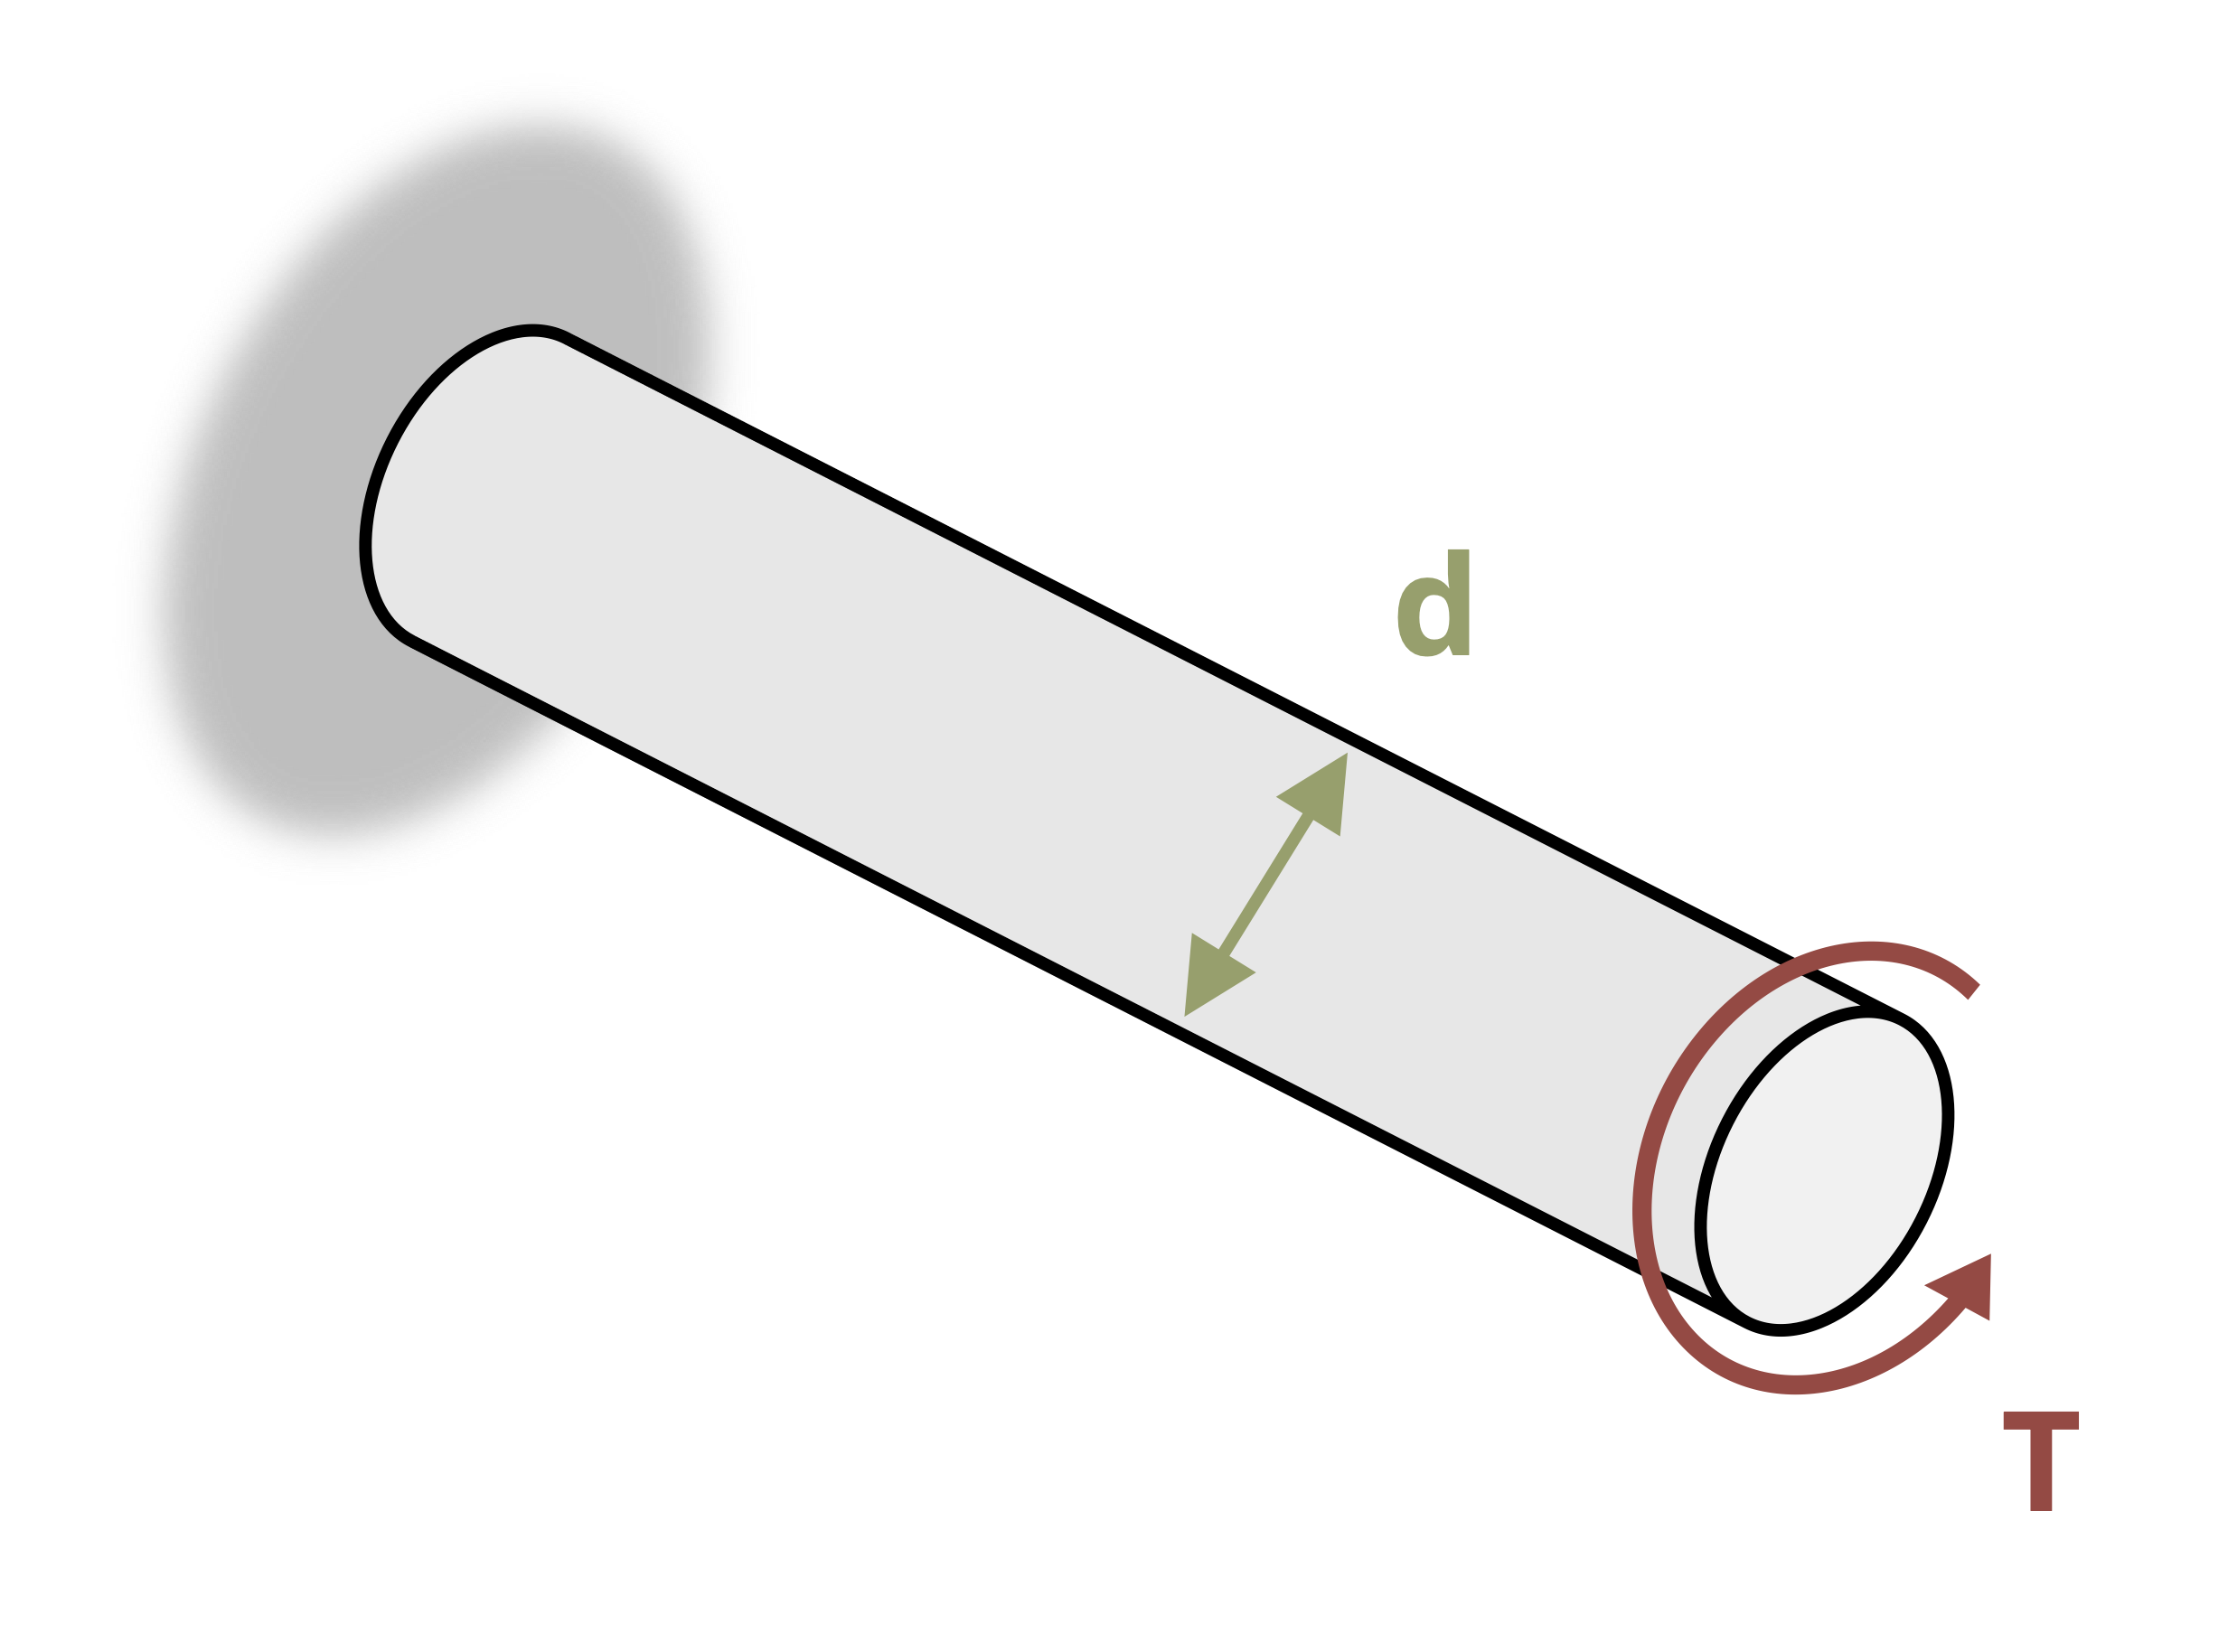
\includegraphics[width=2.60417in,height=\textheight,keepaspectratio]{images/265.png}
{[}Problem adapted from © Kurt Gramoll CC BY NC-SA 4.0{]}

\begin{Shaded}
\begin{Highlighting}[]
\NormalTok{\#| standalone: true}
\NormalTok{\#| viewerHeight: 600}
\NormalTok{\#| components: [viewer]}

\NormalTok{from shiny import App, render, ui, reactive}
\NormalTok{import random}
\NormalTok{import asyncio}
\NormalTok{import io}
\NormalTok{import math}
\NormalTok{import string}
\NormalTok{from datetime import datetime}
\NormalTok{from pathlib import Path}

\NormalTok{def generate\_random\_letters(length):}
\NormalTok{    \# Generate a random string of letters of specified length}
\NormalTok{    return \textquotesingle{}\textquotesingle{}.join(random.choice(string.ascii\_lowercase) for \_ in range(length)) }

\NormalTok{problem\_ID="265"}
\NormalTok{T=reactive.Value("\_\_")}
\NormalTok{d=reactive.Value("\_\_")}


\NormalTok{attempts=["Timestamp,Attempt,Answer,Feedback\textbackslash{}n"]}

\NormalTok{app\_ui = ui.page\_fluid(}
\NormalTok{    ui.markdown("**Please enter your ID number from your instructor and click to generate your problem**"),}
\NormalTok{    ui.input\_text("ID","", placeholder="Enter ID Number Here"),}
\NormalTok{    ui.input\_action\_button("generate\_problem", "Generate Problem", class\_="btn{-}primary"),}
\NormalTok{    ui.markdown("**Problem Statement**"),}
\NormalTok{    ui.output\_ui("ui\_problem\_statement"),}
\NormalTok{    ui.input\_text("answer","Your Answer in units of kN{-}m", placeholder="Please enter your answer"),}
\NormalTok{    ui.input\_action\_button("submit", "Submit Answer", class\_="btn{-}primary"),}
\NormalTok{    ui.download\_button("download", "Download File to Submit", class\_="btn{-}success"),}
\NormalTok{)}


\NormalTok{def server(input, output, session):}
\NormalTok{    \# Initialize a counter for attempts}
\NormalTok{    attempt\_counter = reactive.Value(0)}

\NormalTok{    @output}
\NormalTok{    @render.ui}
\NormalTok{    def ui\_problem\_statement():}
\NormalTok{        return[ui.markdown(f"What torque is required to create a maximum shear stress of τ = \{T()\} MPa in a solid circular bar of diameter d  = \{d()\} mm? .")]}
    
\NormalTok{    @reactive.Effect}
\NormalTok{    @reactive.event(input.generate\_problem)}
\NormalTok{    def randomize\_vars():}
\NormalTok{        random.seed(input.ID())}
\NormalTok{        T.set(random.randrange(20, 50, 1))}
\NormalTok{        d.set(random.randrange(50, 200, 1))}
        
\NormalTok{    @reactive.Effect}
\NormalTok{    @reactive.event(input.submit)}
\NormalTok{    def \_():}
\NormalTok{        attempt\_counter.set(attempt\_counter() + 1)  \# Increment the attempt counter on each submission.}
\NormalTok{        J = (math.pi/2)*(d()/2000)**4}
\NormalTok{        instr= (T()*1000*J)/(d()/2000)}
\NormalTok{        if math.isclose(float(input.answer()), instr, rel\_tol=0.01):}
\NormalTok{            check = "*Correct*"}
\NormalTok{            correct\_indicator = "JL"}
\NormalTok{        else:}
\NormalTok{            check = "*Not Correct.*"}
\NormalTok{            correct\_indicator = "JG"}

\NormalTok{        \# Generate random parts for the encoded attempt.}
\NormalTok{        random\_start = generate\_random\_letters(4)}
\NormalTok{        random\_middle = generate\_random\_letters(4)}
\NormalTok{        random\_end = generate\_random\_letters(4)}
\NormalTok{        encoded\_attempt = f"\{random\_start\}\{problem\_ID\}{-}\{random\_middle\}\{attempt\_counter()\}\{correct\_indicator\}{-}\{random\_end\}\{input.ID()\}"}

\NormalTok{        \# Store the most recent encoded attempt in a reactive value so it persists across submissions}
\NormalTok{        session.encoded\_attempt = reactive.Value(encoded\_attempt)}

\NormalTok{        \# Append the attempt data to the attempts list without the encoded attempt}
\NormalTok{        attempts.append(f"\{datetime.now()\}, \{attempt\_counter()\}, \{input.answer()\}, \{check\}\textbackslash{}n")}

\NormalTok{        \# Show feedback to the user.}
\NormalTok{        feedback = ui.markdown(f"Your answer of \{input.answer()\} is \{check\}.")}
\NormalTok{        m = ui.modal(}
\NormalTok{            feedback,}
\NormalTok{            title="Feedback",}
\NormalTok{            easy\_close=True}
\NormalTok{        )}
\NormalTok{        ui.modal\_show(m)}

\NormalTok{    @session.download(filename=lambda: f"Problem\_Log{-}\{problem\_ID\}{-}\{input.ID()\}.csv")}
\NormalTok{    async def download():}
\NormalTok{        \# Start the CSV with the encoded attempt (without label)}
\NormalTok{        final\_encoded = session.encoded\_attempt() if session.encoded\_attempt is not None else "No attempts"}
\NormalTok{        yield f"\{final\_encoded\}\textbackslash{}n\textbackslash{}n"}
        
\NormalTok{        \# Write the header for the remaining CSV data once}
\NormalTok{        yield "Timestamp,Attempt,Answer,Feedback\textbackslash{}n"}
        
\NormalTok{        \# Write the attempts data, ensure that the header from the attempts list is not written again}
\NormalTok{        for attempt in attempts[1:]:  \# Skip the first element which is the header}
\NormalTok{            await asyncio.sleep(0.25)  \# This delay may not be necessary; adjust as needed}
\NormalTok{            yield attempt}


\NormalTok{\# App installation}
\NormalTok{app = App(app\_ui, server)}
\end{Highlighting}
\end{Shaded}

\chapter*{Problem 6.2 - Torsional
Stress}\label{problem-6.2---torsional-stress}
\addcontentsline{toc}{chapter}{Problem 6.2 - Torsional Stress}

\markboth{Problem 6.2 - Torsional Stress}{Problem 6.2 - Torsional
Stress}

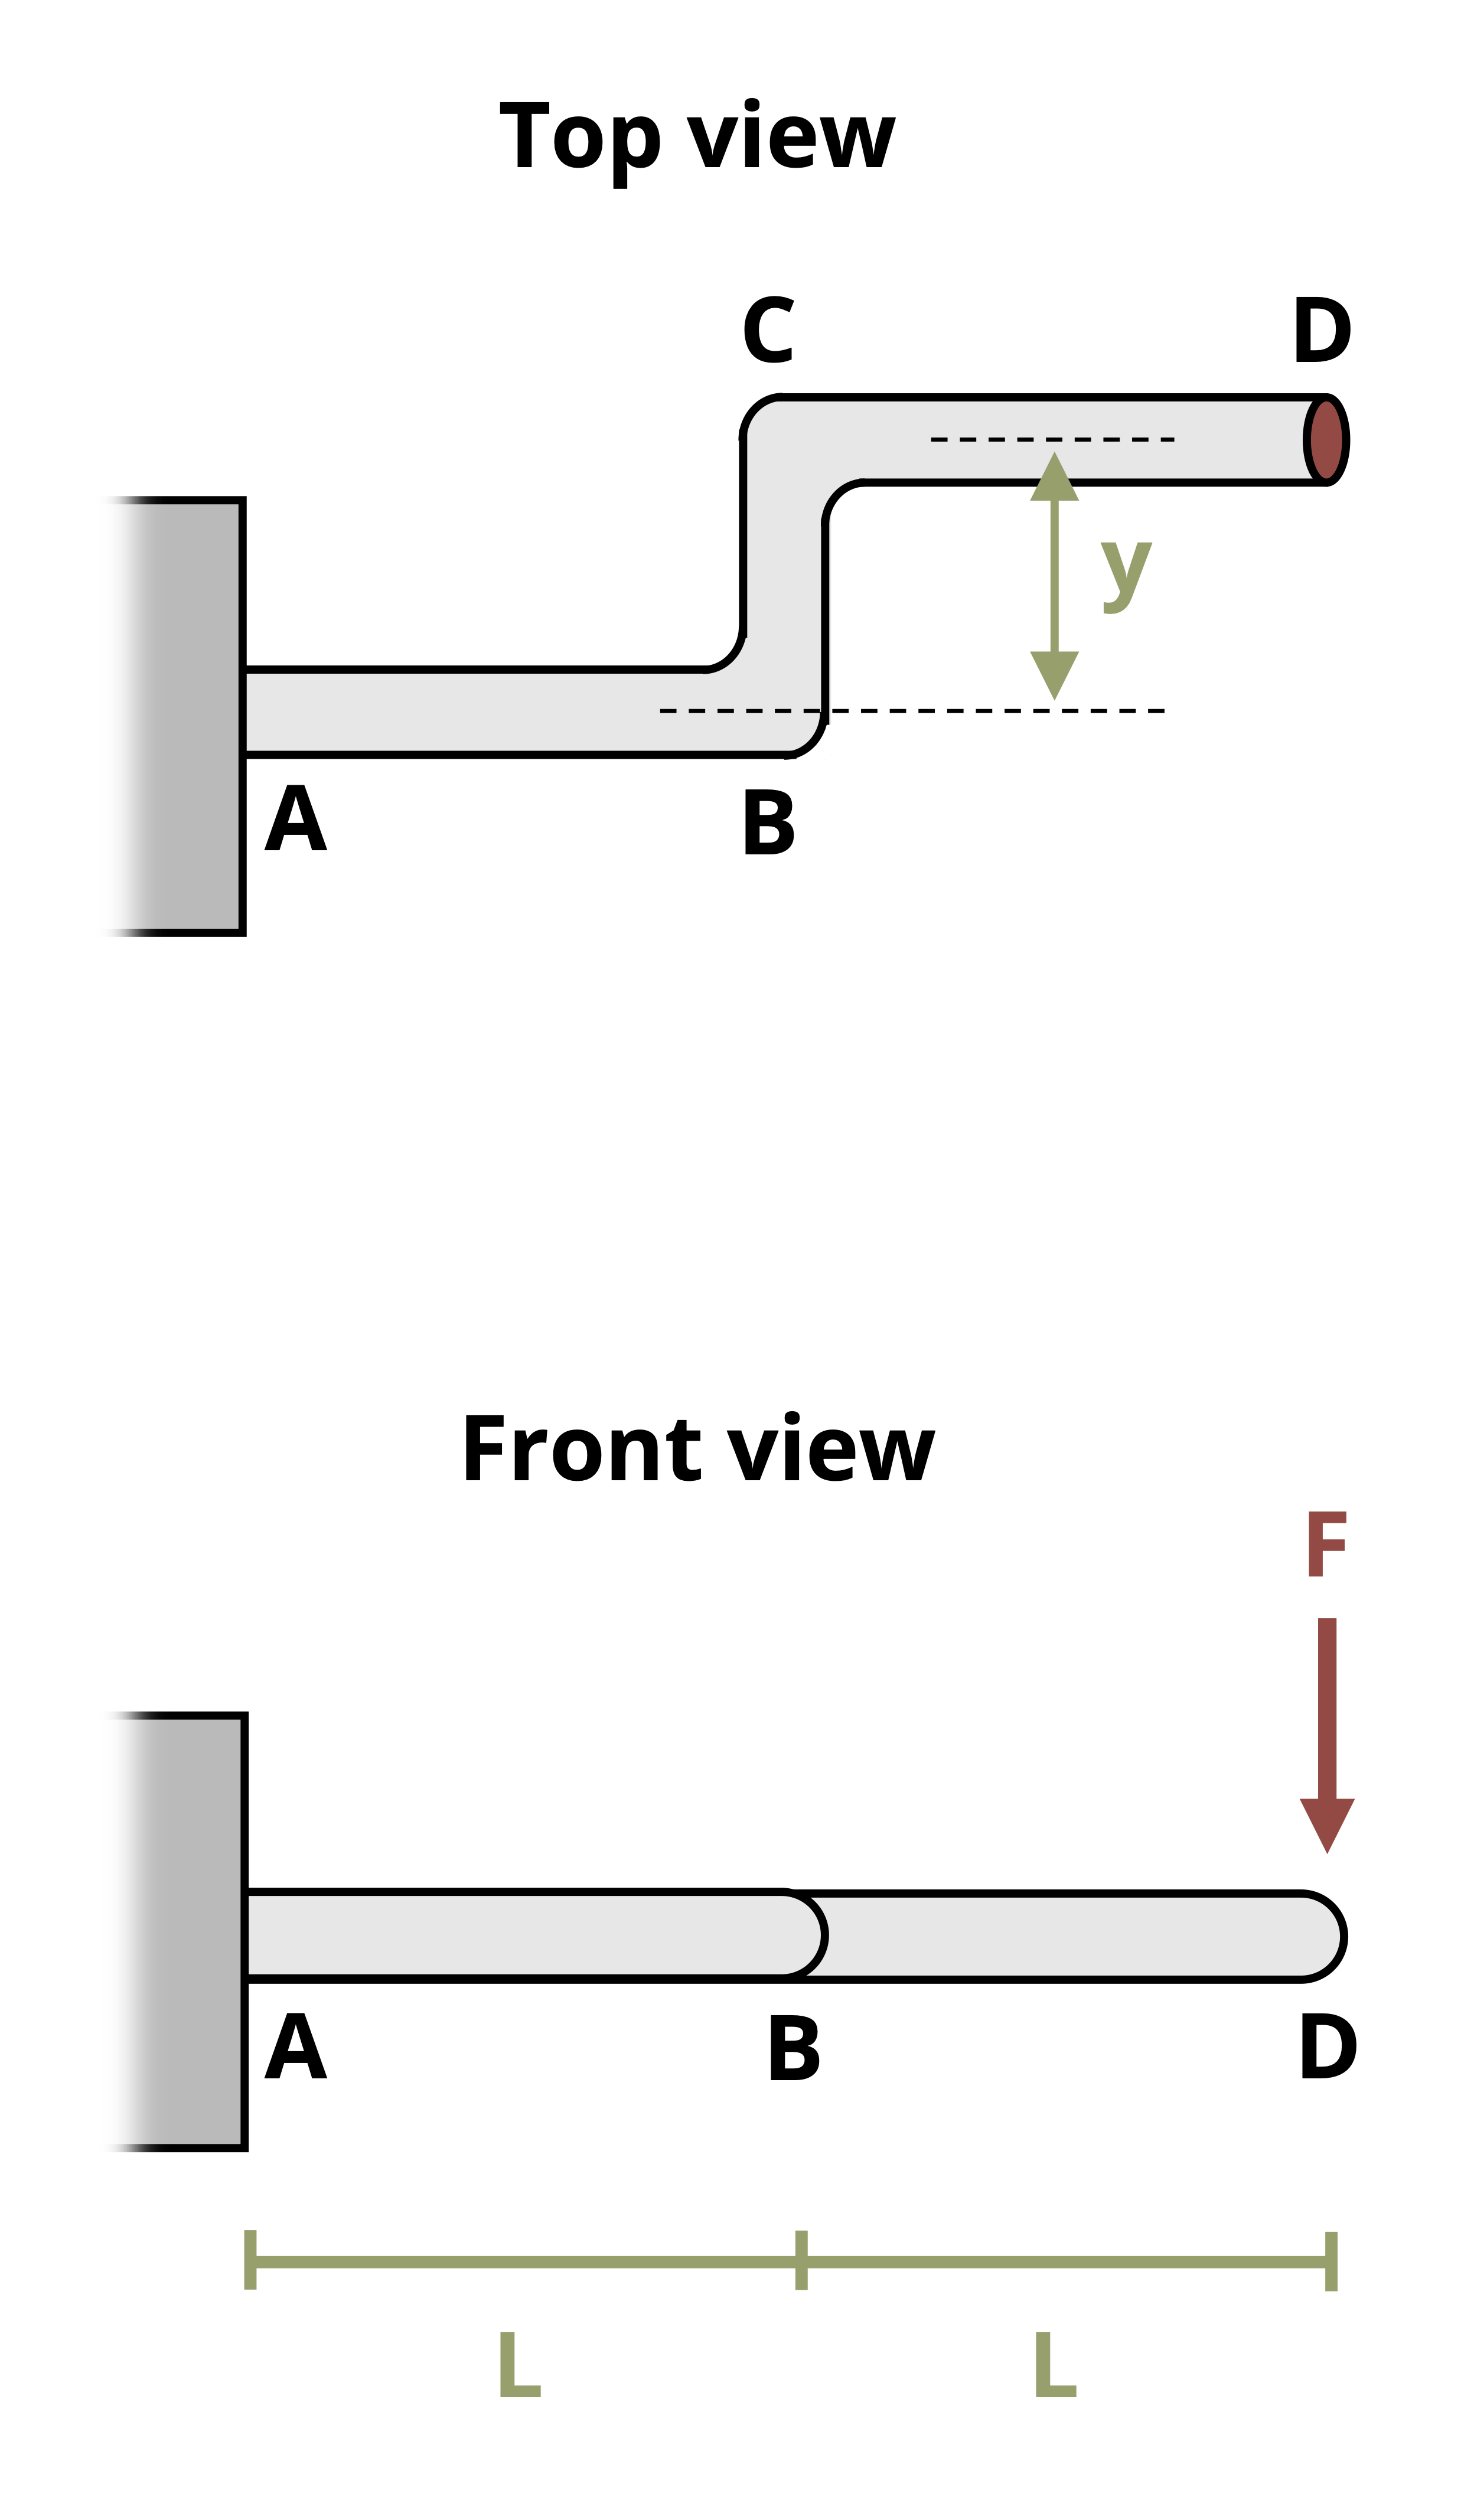
\includegraphics[width=3.125in,height=\textheight,keepaspectratio]{images/267.png}
{[}Problem adapted from © Kurt Gramoll CC BY NC-SA 4.0{]}

\begin{Shaded}
\begin{Highlighting}[]
\NormalTok{\#| standalone: true}
\NormalTok{\#| viewerHeight: 600}
\NormalTok{\#| components: [viewer]}

\NormalTok{from shiny import App, render, ui, reactive}
\NormalTok{import random}
\NormalTok{import asyncio}
\NormalTok{import io}
\NormalTok{import math}
\NormalTok{import string}
\NormalTok{from datetime import datetime}
\NormalTok{from pathlib import Path}

\NormalTok{def generate\_random\_letters(length):}
\NormalTok{    \# Generate a random string of letters of specified length}
\NormalTok{    return \textquotesingle{}\textquotesingle{}.join(random.choice(string.ascii\_lowercase) for \_ in range(length)) }

\NormalTok{problem\_ID="267"}
\NormalTok{F=reactive.Value("\_\_")}
\NormalTok{L=reactive.Value("\_\_")}
\NormalTok{y=reactive.Value("\_\_")}
\NormalTok{d=(reactive.Value("\_\_"))}

\NormalTok{attempts=["Timestamp,Attempt,Answer,Feedback\textbackslash{}n"]}

\NormalTok{app\_ui = ui.page\_fluid(}
\NormalTok{    ui.markdown("**Please enter your ID number from your instructor and click to generate your problem**"),}
\NormalTok{    ui.input\_text("ID","", placeholder="Enter ID Number Here"),}
\NormalTok{    ui.input\_action\_button("generate\_problem", "Generate Problem", class\_="btn{-}primary"),}
\NormalTok{    ui.markdown("**Problem Statement**"),}
\NormalTok{    ui.output\_ui("ui\_problem\_statement"),}
\NormalTok{    ui.input\_text("answer","Your Answer in units of ksi", placeholder="Please enter your answer"),}
\NormalTok{    ui.input\_action\_button("submit", "Submit Answer", class\_="btn{-}primary"),}
\NormalTok{    ui.download\_button("download", "Download File to Submit", class\_="btn{-}success"),}
\NormalTok{)}


\NormalTok{def server(input, output, session):}
\NormalTok{    \# Initialize a counter for attempts}
\NormalTok{    attempt\_counter = reactive.Value(0)}

\NormalTok{    @output}
\NormalTok{    @render.ui}
\NormalTok{    def ui\_problem\_statement():}
\NormalTok{        return[ui.markdown(f"A force F = \{F()\} lb is applied to a hand crank that is stuck and will not turn. If L = \{L()\} in. and y = \{y()\} in., determine the maximum shear stress due to torsion in the crank rod between A and B. Assume the crank has diameter d = \{d()\} in.")]}
    
\NormalTok{    @reactive.Effect}
\NormalTok{    @reactive.event(input.generate\_problem)}
\NormalTok{    def randomize\_vars():}
\NormalTok{        random.seed(input.ID())}
\NormalTok{        F.set(random.randrange(100, 350, 10))}
\NormalTok{        L.set(random.randrange(100, 200, 1)/10)}
\NormalTok{        y.set(round(L()/2, 2))}
\NormalTok{        d.set(random.randrange(3, 15, 1)/10)}
        
\NormalTok{    @reactive.Effect}
\NormalTok{    @reactive.event(input.submit)}
\NormalTok{    def \_():}
\NormalTok{        attempt\_counter.set(attempt\_counter() + 1)  \# Increment the attempt counter on each submission.}
\NormalTok{        T = F()*y()}
\NormalTok{        J = (math.pi/2)*(d()/2)**4}
\NormalTok{        instr= ((T*d()/2)/J)/10**3}
\NormalTok{        if math.isclose(float(input.answer()), instr, rel\_tol=0.01):}
\NormalTok{            check = "*Correct*"}
\NormalTok{            correct\_indicator = "JL"}
\NormalTok{        else:}
\NormalTok{            check = "*Not Correct.*"}
\NormalTok{            correct\_indicator = "JG"}

\NormalTok{        \# Generate random parts for the encoded attempt.}
\NormalTok{        random\_start = generate\_random\_letters(4)}
\NormalTok{        random\_middle = generate\_random\_letters(4)}
\NormalTok{        random\_end = generate\_random\_letters(4)}
\NormalTok{        encoded\_attempt = f"\{random\_start\}\{problem\_ID\}{-}\{random\_middle\}\{attempt\_counter()\}\{correct\_indicator\}{-}\{random\_end\}\{input.ID()\}"}

\NormalTok{        \# Store the most recent encoded attempt in a reactive value so it persists across submissions}
\NormalTok{        session.encoded\_attempt = reactive.Value(encoded\_attempt)}

\NormalTok{        \# Append the attempt data to the attempts list without the encoded attempt}
\NormalTok{        attempts.append(f"\{datetime.now()\}, \{attempt\_counter()\}, \{input.answer()\}, \{check\}\textbackslash{}n")}

\NormalTok{        \# Show feedback to the user.}
\NormalTok{        feedback = ui.markdown(f"Your answer of \{input.answer()\} is \{check\}.")}
\NormalTok{        m = ui.modal(}
\NormalTok{            feedback,}
\NormalTok{            title="Feedback",}
\NormalTok{            easy\_close=True}
\NormalTok{        )}
\NormalTok{        ui.modal\_show(m)}

\NormalTok{    @session.download(filename=lambda: f"Problem\_Log{-}\{problem\_ID\}{-}\{input.ID()\}.csv")}
\NormalTok{    async def download():}
\NormalTok{        \# Start the CSV with the encoded attempt (without label)}
\NormalTok{        final\_encoded = session.encoded\_attempt() if session.encoded\_attempt is not None else "No attempts"}
\NormalTok{        yield f"\{final\_encoded\}\textbackslash{}n\textbackslash{}n"}
        
\NormalTok{        \# Write the header for the remaining CSV data once}
\NormalTok{        yield "Timestamp,Attempt,Answer,Feedback\textbackslash{}n"}
        
\NormalTok{        \# Write the attempts data, ensure that the header from the attempts list is not written again}
\NormalTok{        for attempt in attempts[1:]:  \# Skip the first element which is the header}
\NormalTok{            await asyncio.sleep(0.25)  \# This delay may not be necessary; adjust as needed}
\NormalTok{            yield attempt}


\NormalTok{\# App installation}
\NormalTok{app = App(app\_ui, server)}
\end{Highlighting}
\end{Shaded}

\chapter*{Problem 6.3 - Torsional
Stress}\label{problem-6.3---torsional-stress}
\addcontentsline{toc}{chapter}{Problem 6.3 - Torsional Stress}

\markboth{Problem 6.3 - Torsional Stress}{Problem 6.3 - Torsional
Stress}

\pandocbounded{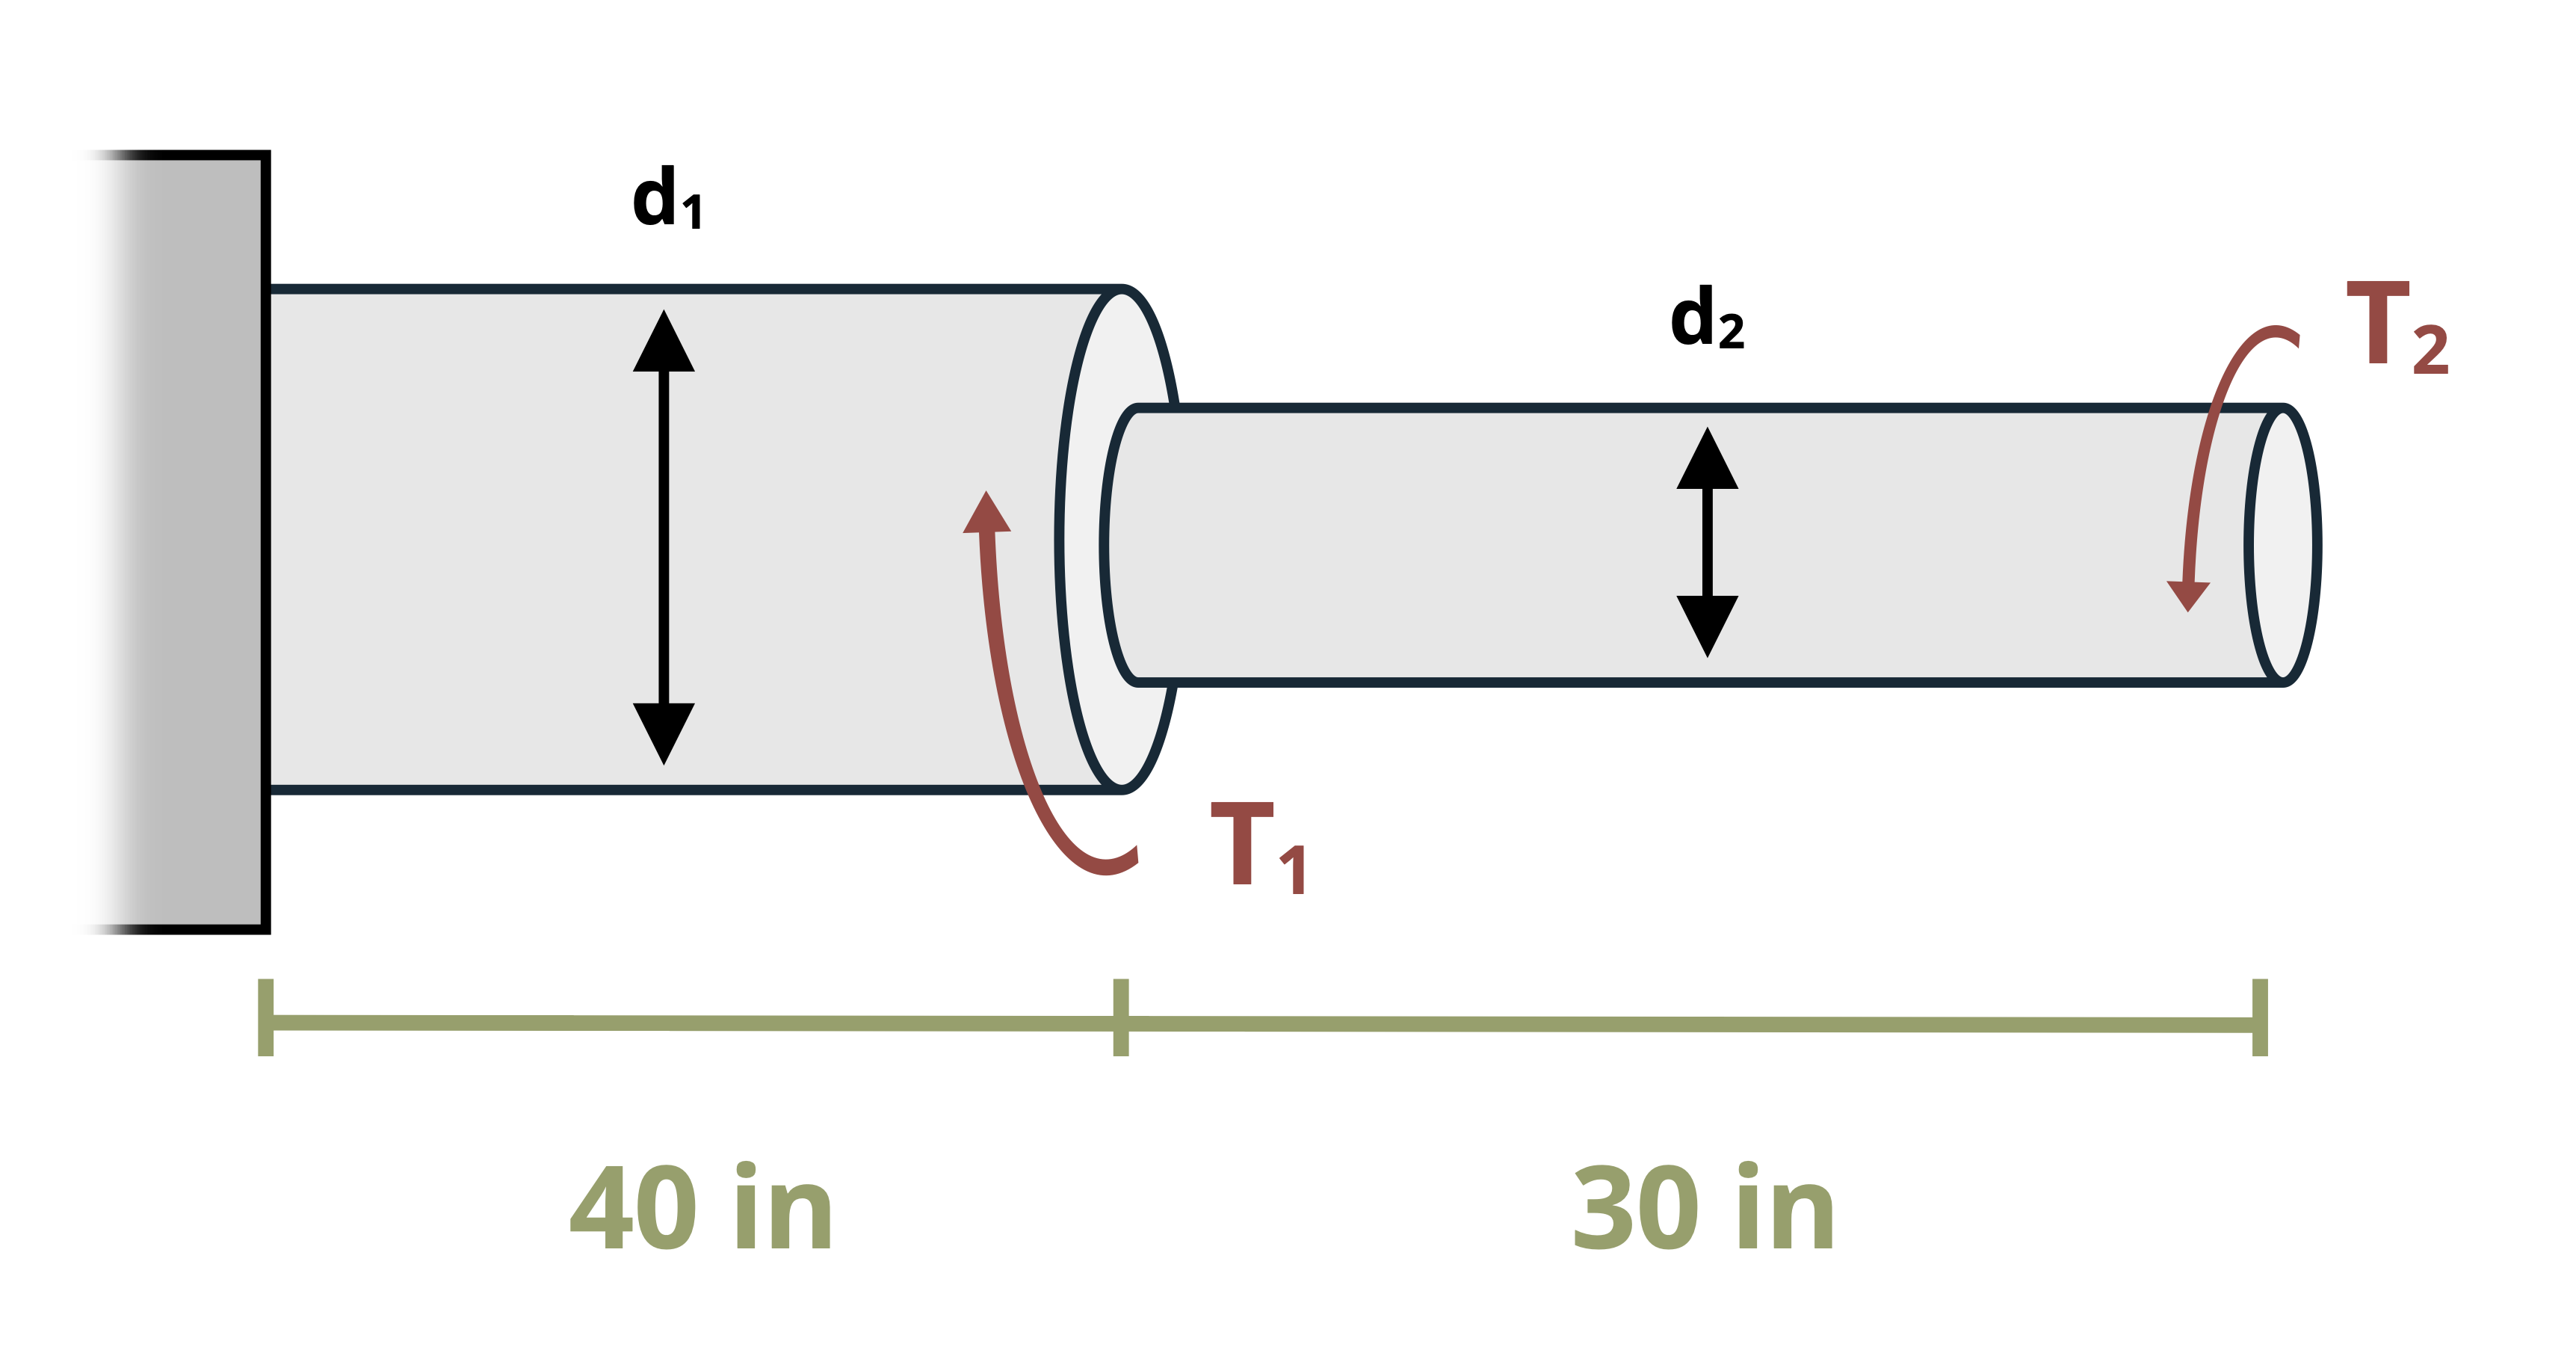
\includegraphics[keepaspectratio]{images/273.png}}
{[}Problem adapted from © Kurt Gramoll CC BY NC-SA 4.0{]}

\begin{Shaded}
\begin{Highlighting}[]
\NormalTok{\#| standalone: true}
\NormalTok{\#| viewerHeight: 600}
\NormalTok{\#| components: [viewer]}

\NormalTok{from shiny import App, render, ui, reactive}
\NormalTok{import random}
\NormalTok{import asyncio}
\NormalTok{import io}
\NormalTok{import math}
\NormalTok{import string}
\NormalTok{from datetime import datetime}
\NormalTok{from pathlib import Path}

\NormalTok{def generate\_random\_letters(length):}
\NormalTok{    \# Generate a random string of letters of specified length}
\NormalTok{    return \textquotesingle{}\textquotesingle{}.join(random.choice(string.ascii\_lowercase) for \_ in range(length)) }

\NormalTok{problem\_ID="273"}
\NormalTok{T1=reactive.Value("\_\_")}
\NormalTok{T2=reactive.Value("\_\_")}
\NormalTok{d1=reactive.Value("\_\_")}
\NormalTok{d2=reactive.Value("\_\_")}

\NormalTok{attempts=["Timestamp,Attempt,Answer,Feedback\textbackslash{}n"]}

\NormalTok{app\_ui = ui.page\_fluid(}
\NormalTok{    ui.markdown("**Please enter your ID number from your instructor and click to generate your problem**"),}
\NormalTok{    ui.input\_text("ID","", placeholder="Enter ID Number Here"),}
\NormalTok{    ui.input\_action\_button("generate\_problem", "Generate Problem", class\_="btn{-}primary"),}
\NormalTok{    ui.markdown("**Problem Statement**"),}
\NormalTok{    ui.output\_ui("ui\_problem\_statement"),}
\NormalTok{    ui.input\_text("answer","Your Answer in units of psi", placeholder="Please enter your answer"),}
\NormalTok{    ui.input\_action\_button("submit", "Submit Answer", class\_="btn{-}primary"),}
\NormalTok{    ui.download\_button("download", "Download File to Submit", class\_="btn{-}success"),}
\NormalTok{)}

\NormalTok{def server(input, output, session):}
\NormalTok{    \# Initialize a counter for attempts}
\NormalTok{    attempt\_counter = reactive.Value(0)}

\NormalTok{    @output}
\NormalTok{    @render.ui}
\NormalTok{    def ui\_problem\_statement():}
\NormalTok{        return[ui.markdown(f"Two torques are applied to a two part circular rod as shown. If T\textless{}sub\textgreater{}1\textless{}/sub\textgreater{} = \{T1()\} kip{-}in., T\textless{}sub\textgreater{}2\textless{}/sub\textgreater{} = \{T2()\} kip{-}in., d\textless{}sub\textgreater{}1\textless{}/sub\textgreater{} = \{d1()\} in., and d\textless{}sub\textgreater{}2\textless{}/sub\textgreater{} = \{d2()\} in., what is the magnitude of the maximum shear stress?")]}
    
\NormalTok{    @reactive.Effect}
\NormalTok{    @reactive.event(input.generate\_problem)}
\NormalTok{    def randomize\_vars():}
\NormalTok{        random.seed(input.ID())}
\NormalTok{        T1.set(random.randrange(5, 50, 1))}
\NormalTok{        T2.set(T1()*random.randrange(3, 5, 1)/10)}
\NormalTok{        d1.set(random.randrange(40, 80, 1)/10)}
\NormalTok{        d2.set(round(d1()*0.8, 2))}
        
\NormalTok{    @reactive.Effect}
\NormalTok{    @reactive.event(input.submit)}
\NormalTok{    def \_():}
\NormalTok{        attempt\_counter.set(attempt\_counter() + 1)  \# Increment the attempt counter on each submission.}
\NormalTok{        F1 = {-}T1()+T2()}
\NormalTok{        F2 = T2()}
\NormalTok{        J1 = (math.pi/2)*(d1()/2)**4}
\NormalTok{        J2 = (math.pi/2)*(d2()/2)**4}
\NormalTok{        tau1 = abs(F1*d1()/2/J1)*1000}
\NormalTok{        tau2 = abs(F2*d2()/2/J2)*1000}
\NormalTok{        if tau1\textgreater{}=tau2:}
\NormalTok{            instr = tau1}
\NormalTok{        else:}
\NormalTok{            instr = tau2}
\NormalTok{        if math.isclose(float(input.answer()), instr, rel\_tol=0.01):}
\NormalTok{            check = "*Correct*"}
\NormalTok{            correct\_indicator = "JL"}
\NormalTok{        else:}
\NormalTok{            check = "*Not Correct.*"}
\NormalTok{            correct\_indicator = "JG"}

\NormalTok{        \# Generate random parts for the encoded attempt.}
\NormalTok{        random\_start = generate\_random\_letters(4)}
\NormalTok{        random\_middle = generate\_random\_letters(4)}
\NormalTok{        random\_end = generate\_random\_letters(4)}
\NormalTok{        encoded\_attempt = f"\{random\_start\}\{problem\_ID\}{-}\{random\_middle\}\{attempt\_counter()\}\{correct\_indicator\}{-}\{random\_end\}\{input.ID()\}"}

\NormalTok{        \# Store the most recent encoded attempt in a reactive value so it persists across submissions}
\NormalTok{        session.encoded\_attempt = reactive.Value(encoded\_attempt)}

\NormalTok{        \# Append the attempt data to the attempts list without the encoded attempt}
\NormalTok{        attempts.append(f"\{datetime.now()\}, \{attempt\_counter()\}, \{input.answer()\}, \{check\}\textbackslash{}n")}

\NormalTok{        \# Show feedback to the user.}
\NormalTok{        feedback = ui.markdown(f"Your answer of \{input.answer()\} is \{check\}.")}
\NormalTok{        m = ui.modal(}
\NormalTok{            feedback,}
\NormalTok{            title="Feedback",}
\NormalTok{            easy\_close=True}
\NormalTok{        )}
\NormalTok{        ui.modal\_show(m)}

\NormalTok{    @session.download(filename=lambda: f"Problem\_Log{-}\{problem\_ID\}{-}\{input.ID()\}.csv")}
\NormalTok{    async def download():}
\NormalTok{        \# Start the CSV with the encoded attempt (without label)}
\NormalTok{        final\_encoded = session.encoded\_attempt() if session.encoded\_attempt is not None else "No attempts"}
\NormalTok{        yield f"\{final\_encoded\}\textbackslash{}n\textbackslash{}n"}
        
\NormalTok{        \# Write the header for the remaining CSV data once}
\NormalTok{        yield "Timestamp,Attempt,Answer,Feedback\textbackslash{}n"}
        
\NormalTok{        \# Write the attempts data, ensure that the header from the attempts list is not written again}
\NormalTok{        for attempt in attempts[1:]:  \# Skip the first element which is the header}
\NormalTok{            await asyncio.sleep(0.25)  \# This delay may not be necessary; adjust as needed}
\NormalTok{            yield attempt}

\NormalTok{\# App installation}
\NormalTok{app = App(app\_ui, server)}
\end{Highlighting}
\end{Shaded}

\chapter*{Problem 6.4 - Torsional
Stress}\label{problem-6.4---torsional-stress}
\addcontentsline{toc}{chapter}{Problem 6.4 - Torsional Stress}

\markboth{Problem 6.4 - Torsional Stress}{Problem 6.4 - Torsional
Stress}

\begin{figure}[H]

{\centering \pandocbounded{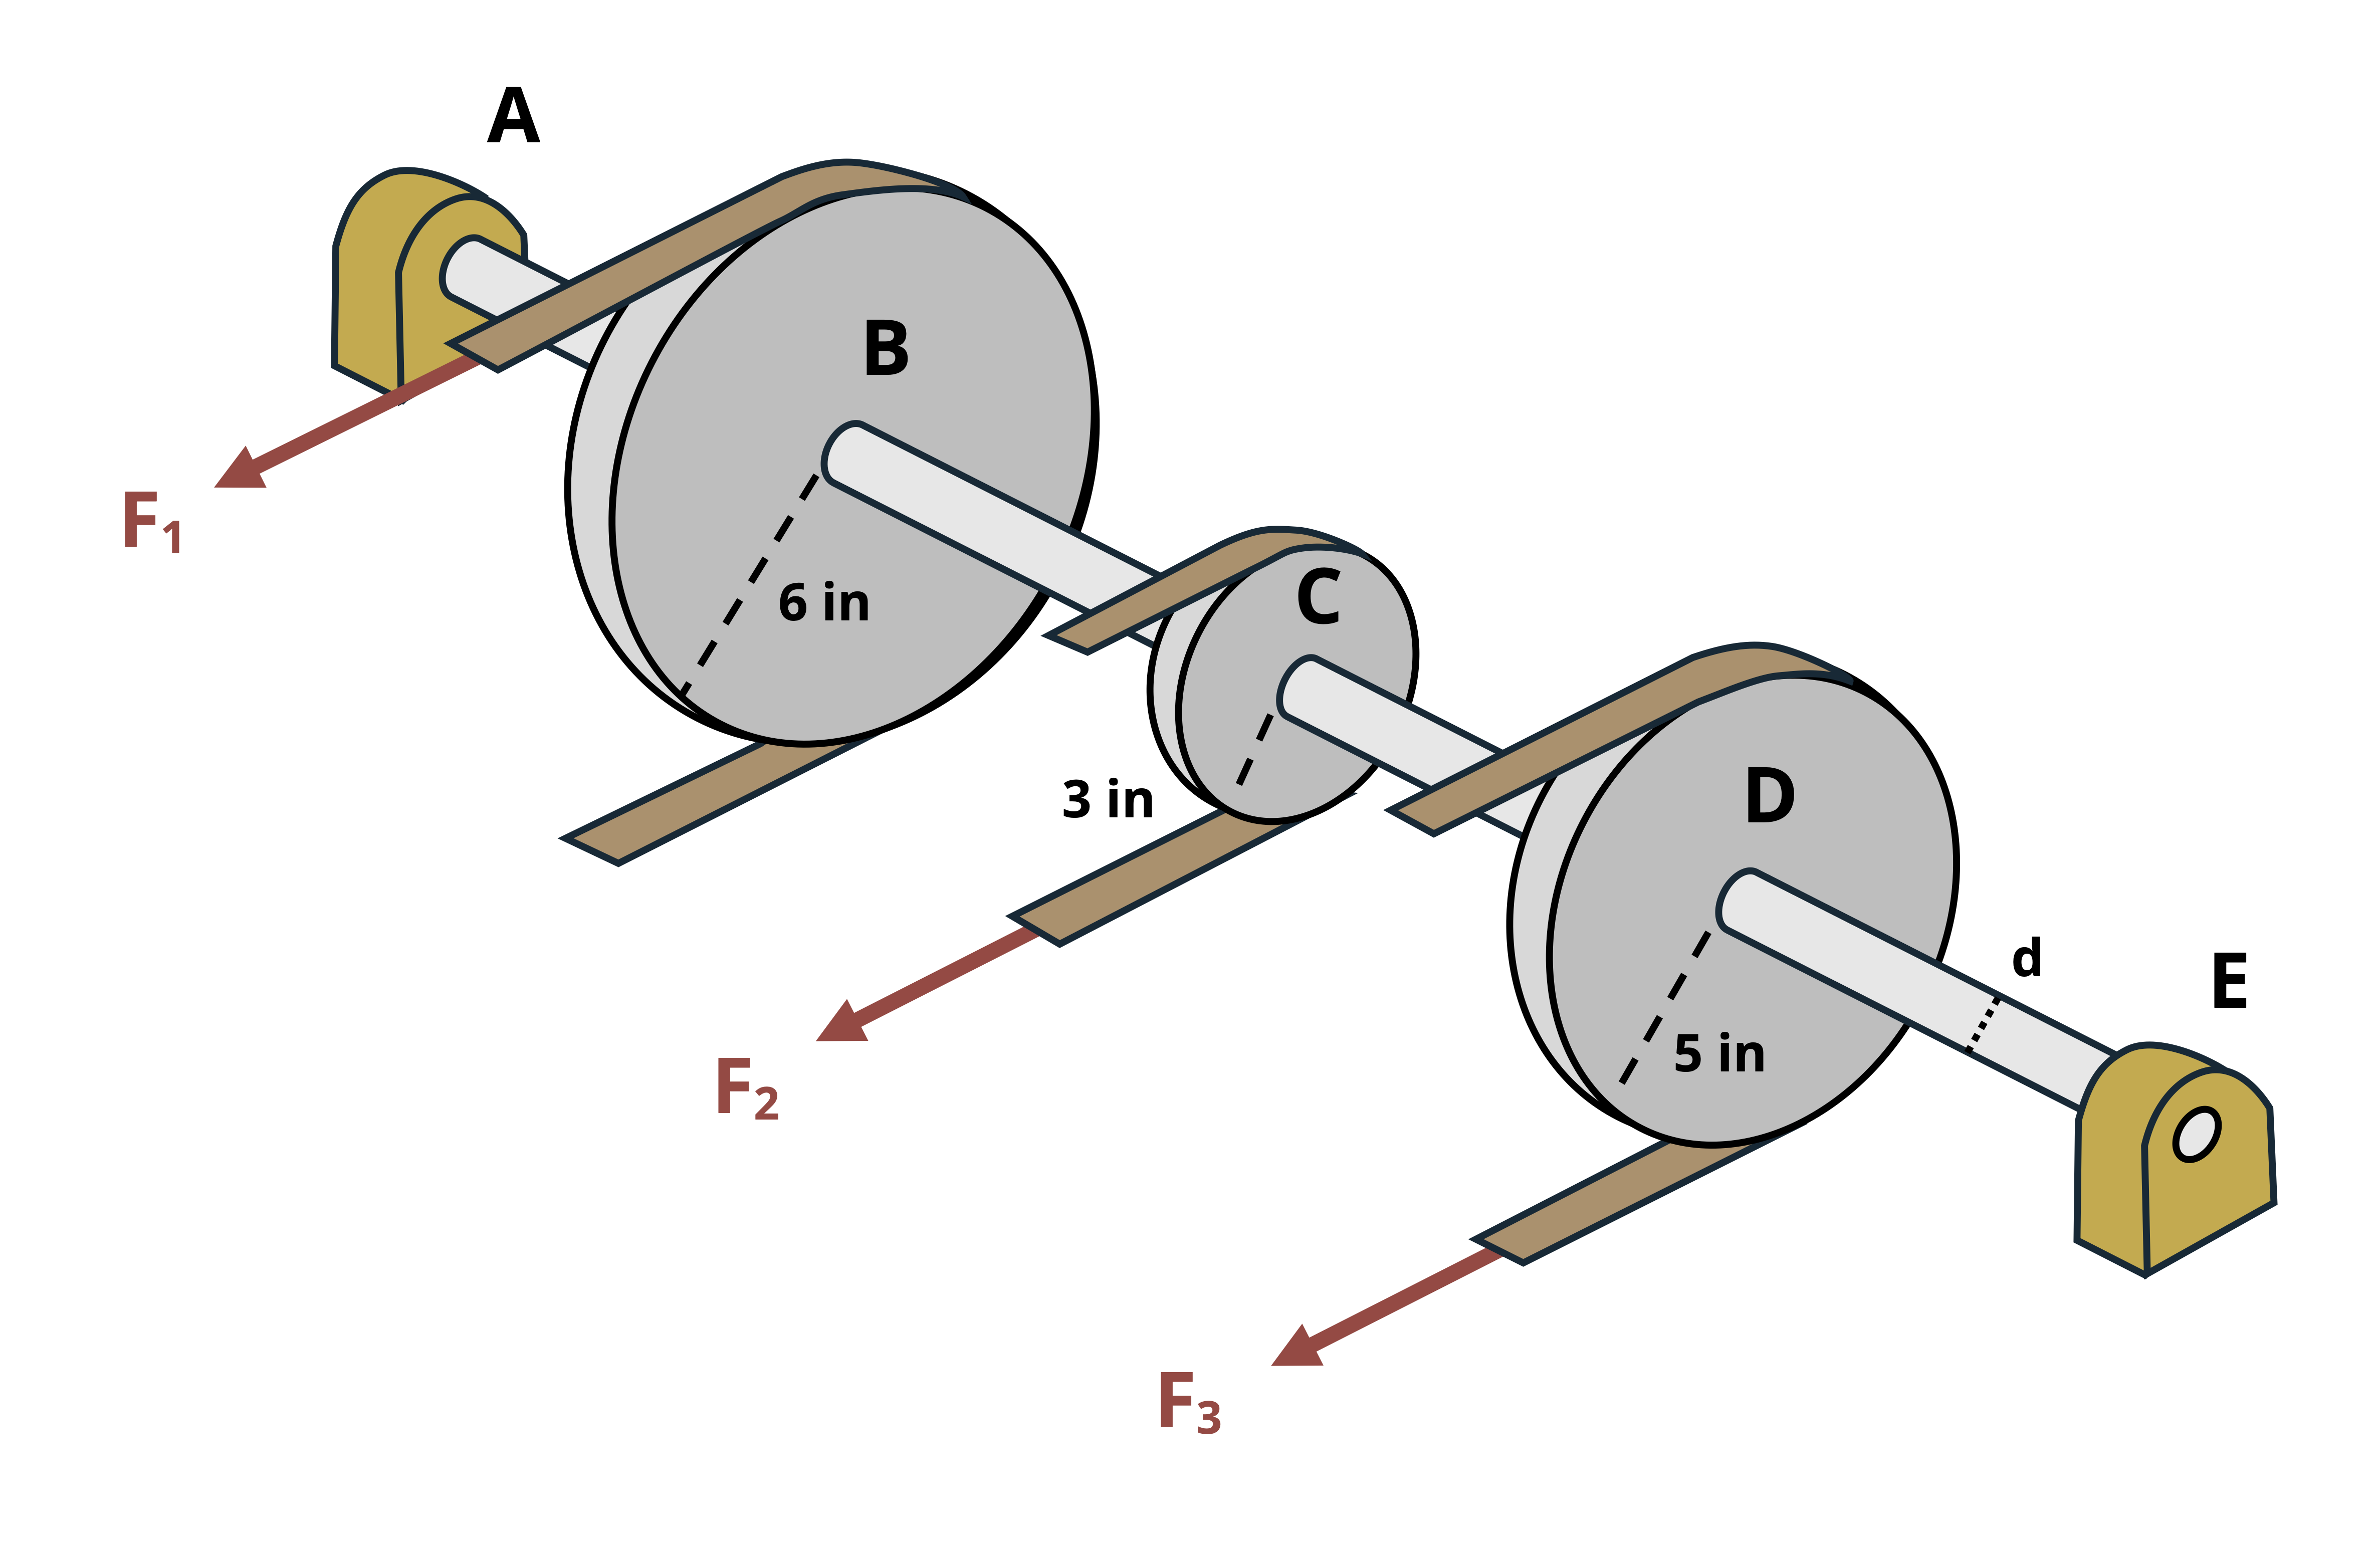
\includegraphics[keepaspectratio]{images/276.png}}

}

\caption{Figure 1: Three belt pullets are connected to a solid shaft.}

\end{figure}%

{[}Problem adapted from © Kurt Gramoll CC BY NC-SA 4.0{]}

\begin{Shaded}
\begin{Highlighting}[]
\NormalTok{\#| standalone: true}
\NormalTok{\#| viewerHeight: 600}
\NormalTok{\#| components: [viewer]}

\NormalTok{from shiny import App, render, ui, reactive}
\NormalTok{import random}
\NormalTok{import asyncio}
\NormalTok{import io}
\NormalTok{import math}
\NormalTok{import string}
\NormalTok{from datetime import datetime}
\NormalTok{from pathlib import Path}

\NormalTok{def generate\_random\_letters(length):}
\NormalTok{    \# Generate a random string of letters of specified length}
\NormalTok{    return \textquotesingle{}\textquotesingle{}.join(random.choice(string.ascii\_lowercase) for \_ in range(length)) }

\NormalTok{problem\_ID="276"}
\NormalTok{d=reactive.Value("\_\_")}
\NormalTok{F1=reactive.Value("\_\_")}
\NormalTok{F2=reactive.Value("\_\_")}
\NormalTok{F3=reactive.Value("\_\_")}

\NormalTok{attempts=["Timestamp,Attempt,Answer,Feedback\textbackslash{}n"]}

\NormalTok{app\_ui = ui.page\_fluid(}
\NormalTok{    ui.markdown("**Please enter your ID number from your instructor and click to generate your problem**"),}
\NormalTok{    ui.input\_text("ID","", placeholder="Enter ID Number Here"),}
\NormalTok{    ui.input\_action\_button("generate\_problem", "Generate Problem", class\_="btn{-}primary"),}
\NormalTok{    ui.markdown("**Problem Statement**"),}
\NormalTok{    ui.output\_ui("ui\_problem\_statement"),}
\NormalTok{    ui.input\_text("answer","Your Answer in units of ksi", placeholder="Please enter your answer"),}
\NormalTok{    ui.input\_action\_button("submit", "Submit Answer", class\_="btn{-}primary"),}
\NormalTok{    ui.download\_button("download", "Download File to Submit", class\_="btn{-}success"),}
\NormalTok{)}


\NormalTok{def server(input, output, session):}
\NormalTok{    \# Initialize a counter for attempts}
\NormalTok{    attempt\_counter = reactive.Value(0)}

\NormalTok{    @output}
\NormalTok{    @render.ui}
\NormalTok{    def ui\_problem\_statement():}
\NormalTok{        return[ui.markdown(f"Three belt pulleys are connected to a solid circular shaft of diameter d = \{d()\} in. that rotates freely at joints A and E. The pulleys are subjected to forces F\textless{}sub\textgreater{}1\textless{}/sub\textgreater{} = \{F1()\} kips, F\textless{}sub\textgreater{}2\textless{}/sub\textgreater{} = \{F2()\} kips, and F\textless{}sub\textgreater{}3\textless{}/sub\textgreater{} = \{F3()\} kips. What is the maximum shear stress in the shaft between pulleys B and C?")]}
    
\NormalTok{    @reactive.Effect}
\NormalTok{    @reactive.event(input.generate\_problem)}
\NormalTok{    def randomize\_vars():}
\NormalTok{        random.seed(input.ID())}
\NormalTok{        d.set(random.randrange(20, 40, 1)/10)}
\NormalTok{        F1.set(random.randrange(20, 200, 2)/10)}
\NormalTok{        F2.set(F1()/2)}
\NormalTok{        F3.set(round(F1()*0.9, 2))}
        
        
\NormalTok{    @reactive.Effect}
\NormalTok{    @reactive.event(input.submit)}
\NormalTok{    def \_():}
\NormalTok{        attempt\_counter.set(attempt\_counter() + 1)  \# Increment the attempt counter on each submission.}
\NormalTok{        T = 6*F1()}
\NormalTok{        instr= (T*(d()/2))/((math.pi/2)*(d()/2)**4)}
\NormalTok{        if math.isclose(float(input.answer()), instr, rel\_tol=0.01):}
\NormalTok{            check = "*Correct*"}
\NormalTok{            correct\_indicator = "JL"}
\NormalTok{        else:}
\NormalTok{            check = "*Not Correct.*"}
\NormalTok{            correct\_indicator = "JG"}

\NormalTok{        \# Generate random parts for the encoded attempt.}
\NormalTok{        random\_start = generate\_random\_letters(4)}
\NormalTok{        random\_middle = generate\_random\_letters(4)}
\NormalTok{        random\_end = generate\_random\_letters(4)}
\NormalTok{        encoded\_attempt = f"\{random\_start\}\{problem\_ID\}{-}\{random\_middle\}\{attempt\_counter()\}\{correct\_indicator\}{-}\{random\_end\}\{input.ID()\}"}

\NormalTok{        \# Store the most recent encoded attempt in a reactive value so it persists across submissions}
\NormalTok{        session.encoded\_attempt = reactive.Value(encoded\_attempt)}

\NormalTok{        \# Append the attempt data to the attempts list without the encoded attempt}
\NormalTok{        attempts.append(f"\{datetime.now()\}, \{attempt\_counter()\}, \{input.answer()\}, \{check\}\textbackslash{}n")}

\NormalTok{        \# Show feedback to the user.}
\NormalTok{        feedback = ui.markdown(f"Your answer of \{input.answer()\} is \{check\}.")}
\NormalTok{        m = ui.modal(}
\NormalTok{            feedback,}
\NormalTok{            title="Feedback",}
\NormalTok{            easy\_close=True}
\NormalTok{        )}
\NormalTok{        ui.modal\_show(m)}

\NormalTok{    @session.download(filename=lambda: f"Problem\_Log{-}\{problem\_ID\}{-}\{input.ID()\}.csv")}
\NormalTok{    async def download():}
\NormalTok{        \# Start the CSV with the encoded attempt (without label)}
\NormalTok{        final\_encoded = session.encoded\_attempt() if session.encoded\_attempt is not None else "No attempts"}
\NormalTok{        yield f"\{final\_encoded\}\textbackslash{}n\textbackslash{}n"}
        
\NormalTok{        \# Write the header for the remaining CSV data once}
\NormalTok{        yield "Timestamp,Attempt,Answer,Feedback\textbackslash{}n"}
        
\NormalTok{        \# Write the attempts data, ensure that the header from the attempts list is not written again}
\NormalTok{        for attempt in attempts[1:]:  \# Skip the first element which is the header}
\NormalTok{            await asyncio.sleep(0.25)  \# This delay may not be necessary; adjust as needed}
\NormalTok{            yield attempt}


\NormalTok{\# App installation}
\NormalTok{app = App(app\_ui, server)}
\end{Highlighting}
\end{Shaded}

\chapter*{Problem 6.5 - Torsional
Stress}\label{problem-6.5---torsional-stress}
\addcontentsline{toc}{chapter}{Problem 6.5 - Torsional Stress}

\markboth{Problem 6.5 - Torsional Stress}{Problem 6.5 - Torsional
Stress}

This is a dynamic rendering of the problem with dynamic variables based
on the username entered.

\pandocbounded{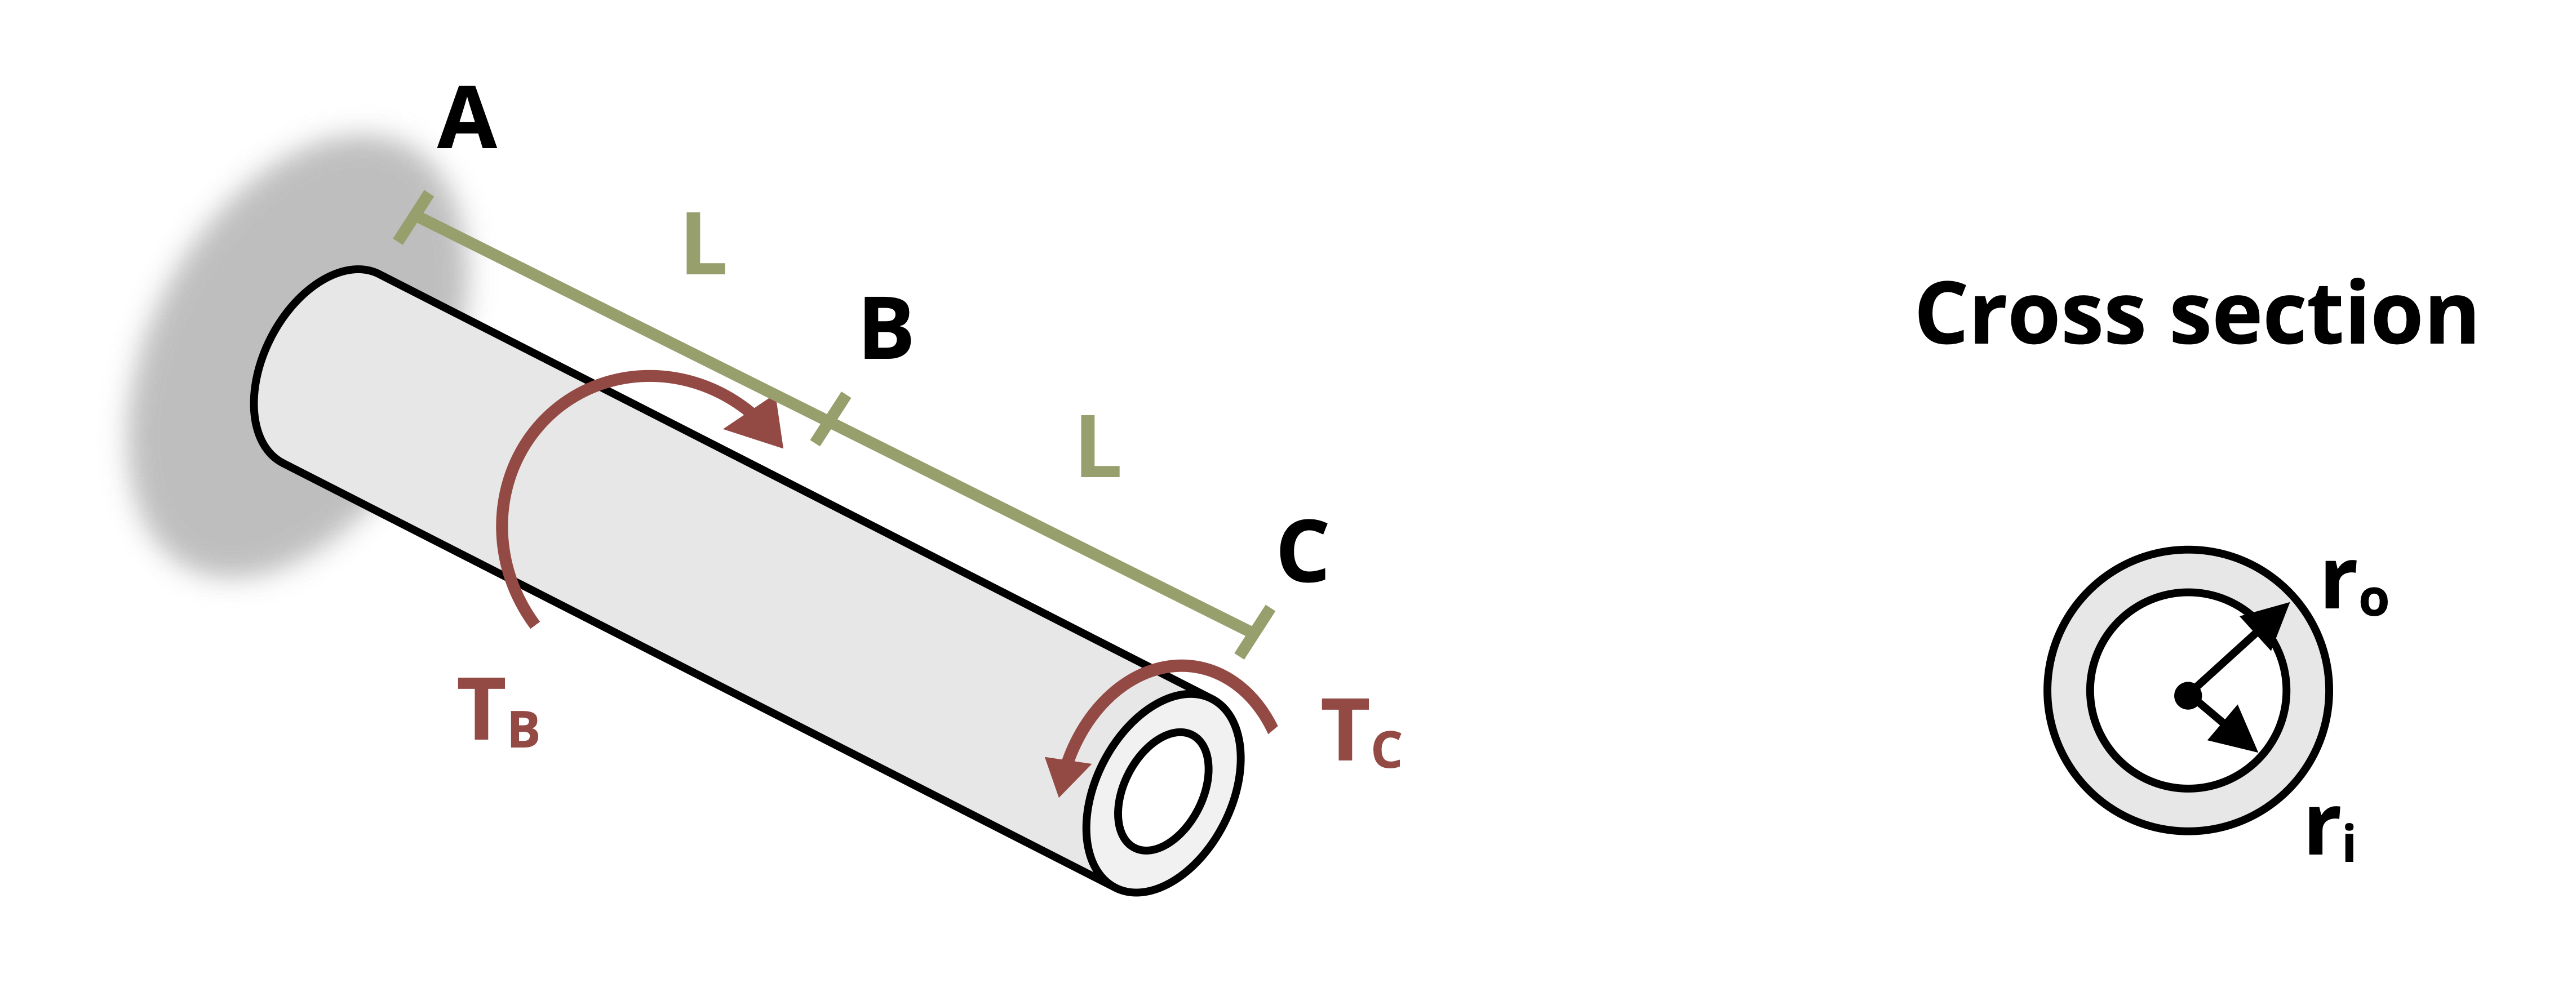
\includegraphics[keepaspectratio]{images/278.png}}
{[}Problem adapted from © Kurt Gramoll CC BY NC-SA 4.0{]}

\begin{Shaded}
\begin{Highlighting}[]
\NormalTok{\#| standalone: true}
\NormalTok{\#| viewerHeight: 600}
\NormalTok{\#| components: [viewer]}

\NormalTok{from shiny import App, render, ui, reactive}
\NormalTok{import random}
\NormalTok{import asyncio}
\NormalTok{import io}
\NormalTok{import math}
\NormalTok{import string}
\NormalTok{from datetime import datetime}
\NormalTok{from pathlib import Path}

\NormalTok{def generate\_random\_letters(length):}
\NormalTok{    \# Generate a random string of letters of specified length}
\NormalTok{    return \textquotesingle{}\textquotesingle{}.join(random.choice(string.ascii\_lowercase) for \_ in range(length)) }

\NormalTok{problem\_ID="278"}
\NormalTok{ro=reactive.Value("\_\_")}
\NormalTok{ri=reactive.Value("\_\_")}
\NormalTok{TB=reactive.Value("\_\_")}
\NormalTok{TC=reactive.Value("\_\_")}
\NormalTok{L=reactive.Value("\_\_")}

\NormalTok{attempts=["Timestamp,Attempt,Answer,Feedback\textbackslash{}n"]}

\NormalTok{app\_ui = ui.page\_fluid(}
\NormalTok{    ui.markdown("**Please enter your ID number from your instructor and click to generate your problem**"),}
\NormalTok{    ui.input\_text("ID","", placeholder="Enter ID Number Here"),}
\NormalTok{    ui.input\_action\_button("generate\_problem", "Generate Problem", class\_="btn{-}primary"),}
\NormalTok{    ui.markdown("**Problem Statement**"),}
\NormalTok{    ui.output\_ui("ui\_problem\_statement"),}
\NormalTok{    ui.input\_text("answer","Your Answer in units of ksi", placeholder="Please enter your answer"),}
\NormalTok{    ui.input\_action\_button("submit", "Submit Answer", class\_="btn{-}primary"),}
\NormalTok{    ui.download\_button("download", "Download File to Submit", class\_="btn{-}success"),}
\NormalTok{)}


\NormalTok{def server(input, output, session):}
\NormalTok{    \# Initialize a counter for attempts}
\NormalTok{    attempt\_counter = reactive.Value(0)}

\NormalTok{    @output}
\NormalTok{    @render.ui}
\NormalTok{    def ui\_problem\_statement():}
\NormalTok{        return[ui.markdown(f"Two torques ,T\textless{}sub\textgreater{}B\textless{}/sub\textgreater{} = \{TB()\} kip{-}ft and T\textless{}sub\textgreater{}C\textless{}/sub\textgreater{} = \{TC()\} kip{-}ft, are applied to the hollow pipe as shown. If L = \{L()\} ft., r\textless{}sub\textgreater{}o\textless{}/sub\textgreater{} = \{ro()\} in., and r\textless{}sub\textgreater{}i\textless{}/sub\textgreater{} = \{ri()\} in., determine the maximum shear stress in the pipe.")]}
    
\NormalTok{    @reactive.Effect}
\NormalTok{    @reactive.event(input.generate\_problem)}
\NormalTok{    def randomize\_vars():}
\NormalTok{        random.seed(input.ID())}
\NormalTok{        TB.set(random.randrange(100, 500, 100))}
\NormalTok{        TC.set(TB()/2)}
\NormalTok{        L.set(random.randrange(10, 90, 1)/10)}
\NormalTok{        ro.set(random.randrange(15, 60, 1)/10)}
\NormalTok{        ri.set(round(ro()*0.8))}
        
        
\NormalTok{    @reactive.Effect}
\NormalTok{    @reactive.event(input.submit)}
\NormalTok{    def \_():}
\NormalTok{        attempt\_counter.set(attempt\_counter() + 1)  \# Increment the attempt counter on each submission.}
\NormalTok{        Tmax = (TB(){-}TC())*12}
\NormalTok{        J = (math.pi/2)*(ro()**4 {-} ri()**4)}
\NormalTok{        instr= (Tmax*ro())/J}
\NormalTok{        if math.isclose(float(input.answer()), instr, rel\_tol=0.01):}
\NormalTok{            check = "*Correct*"}
\NormalTok{            correct\_indicator = "JL"}
\NormalTok{        else:}
\NormalTok{            check = "*Not Correct.*"}
\NormalTok{            correct\_indicator = "JG"}

\NormalTok{        \# Generate random parts for the encoded attempt.}
\NormalTok{        random\_start = generate\_random\_letters(4)}
\NormalTok{        random\_middle = generate\_random\_letters(4)}
\NormalTok{        random\_end = generate\_random\_letters(4)}
\NormalTok{        encoded\_attempt = f"\{random\_start\}\{problem\_ID\}{-}\{random\_middle\}\{attempt\_counter()\}\{correct\_indicator\}{-}\{random\_end\}\{input.ID()\}"}

\NormalTok{        \# Store the most recent encoded attempt in a reactive value so it persists across submissions}
\NormalTok{        session.encoded\_attempt = reactive.Value(encoded\_attempt)}

\NormalTok{        \# Append the attempt data to the attempts list without the encoded attempt}
\NormalTok{        attempts.append(f"\{datetime.now()\}, \{attempt\_counter()\}, \{input.answer()\}, \{check\}\textbackslash{}n")}

\NormalTok{        \# Show feedback to the user.}
\NormalTok{        feedback = ui.markdown(f"Your answer of \{input.answer()\} is \{check\}.")}
\NormalTok{        m = ui.modal(}
\NormalTok{            feedback,}
\NormalTok{            title="Feedback",}
\NormalTok{            easy\_close=True}
\NormalTok{        )}
\NormalTok{        ui.modal\_show(m)}

\NormalTok{    @session.download(filename=lambda: f"Problem\_Log{-}\{problem\_ID\}{-}\{input.ID()\}.csv")}
\NormalTok{    async def download():}
\NormalTok{        \# Start the CSV with the encoded attempt (without label)}
\NormalTok{        final\_encoded = session.encoded\_attempt() if session.encoded\_attempt is not None else "No attempts"}
\NormalTok{        yield f"\{final\_encoded\}\textbackslash{}n\textbackslash{}n"}
        
\NormalTok{        \# Write the header for the remaining CSV data once}
\NormalTok{        yield "Timestamp,Attempt,Answer,Feedback\textbackslash{}n"}
        
\NormalTok{        \# Write the attempts data, ensure that the header from the attempts list is not written again}
\NormalTok{        for attempt in attempts[1:]:  \# Skip the first element which is the header}
\NormalTok{            await asyncio.sleep(0.25)  \# This delay may not be necessary; adjust as needed}
\NormalTok{            yield attempt}

\NormalTok{\# App installation}
\NormalTok{app = App(app\_ui, server)}
\end{Highlighting}
\end{Shaded}

\chapter*{Problem 6.11 - Torsional
Deformation}\label{problem-6.11---torsional-deformation}
\addcontentsline{toc}{chapter}{Problem 6.11 - Torsional Deformation}

\markboth{Problem 6.11 - Torsional Deformation}{Problem 6.11 - Torsional
Deformation}

\begin{figure}[H]

{\centering \pandocbounded{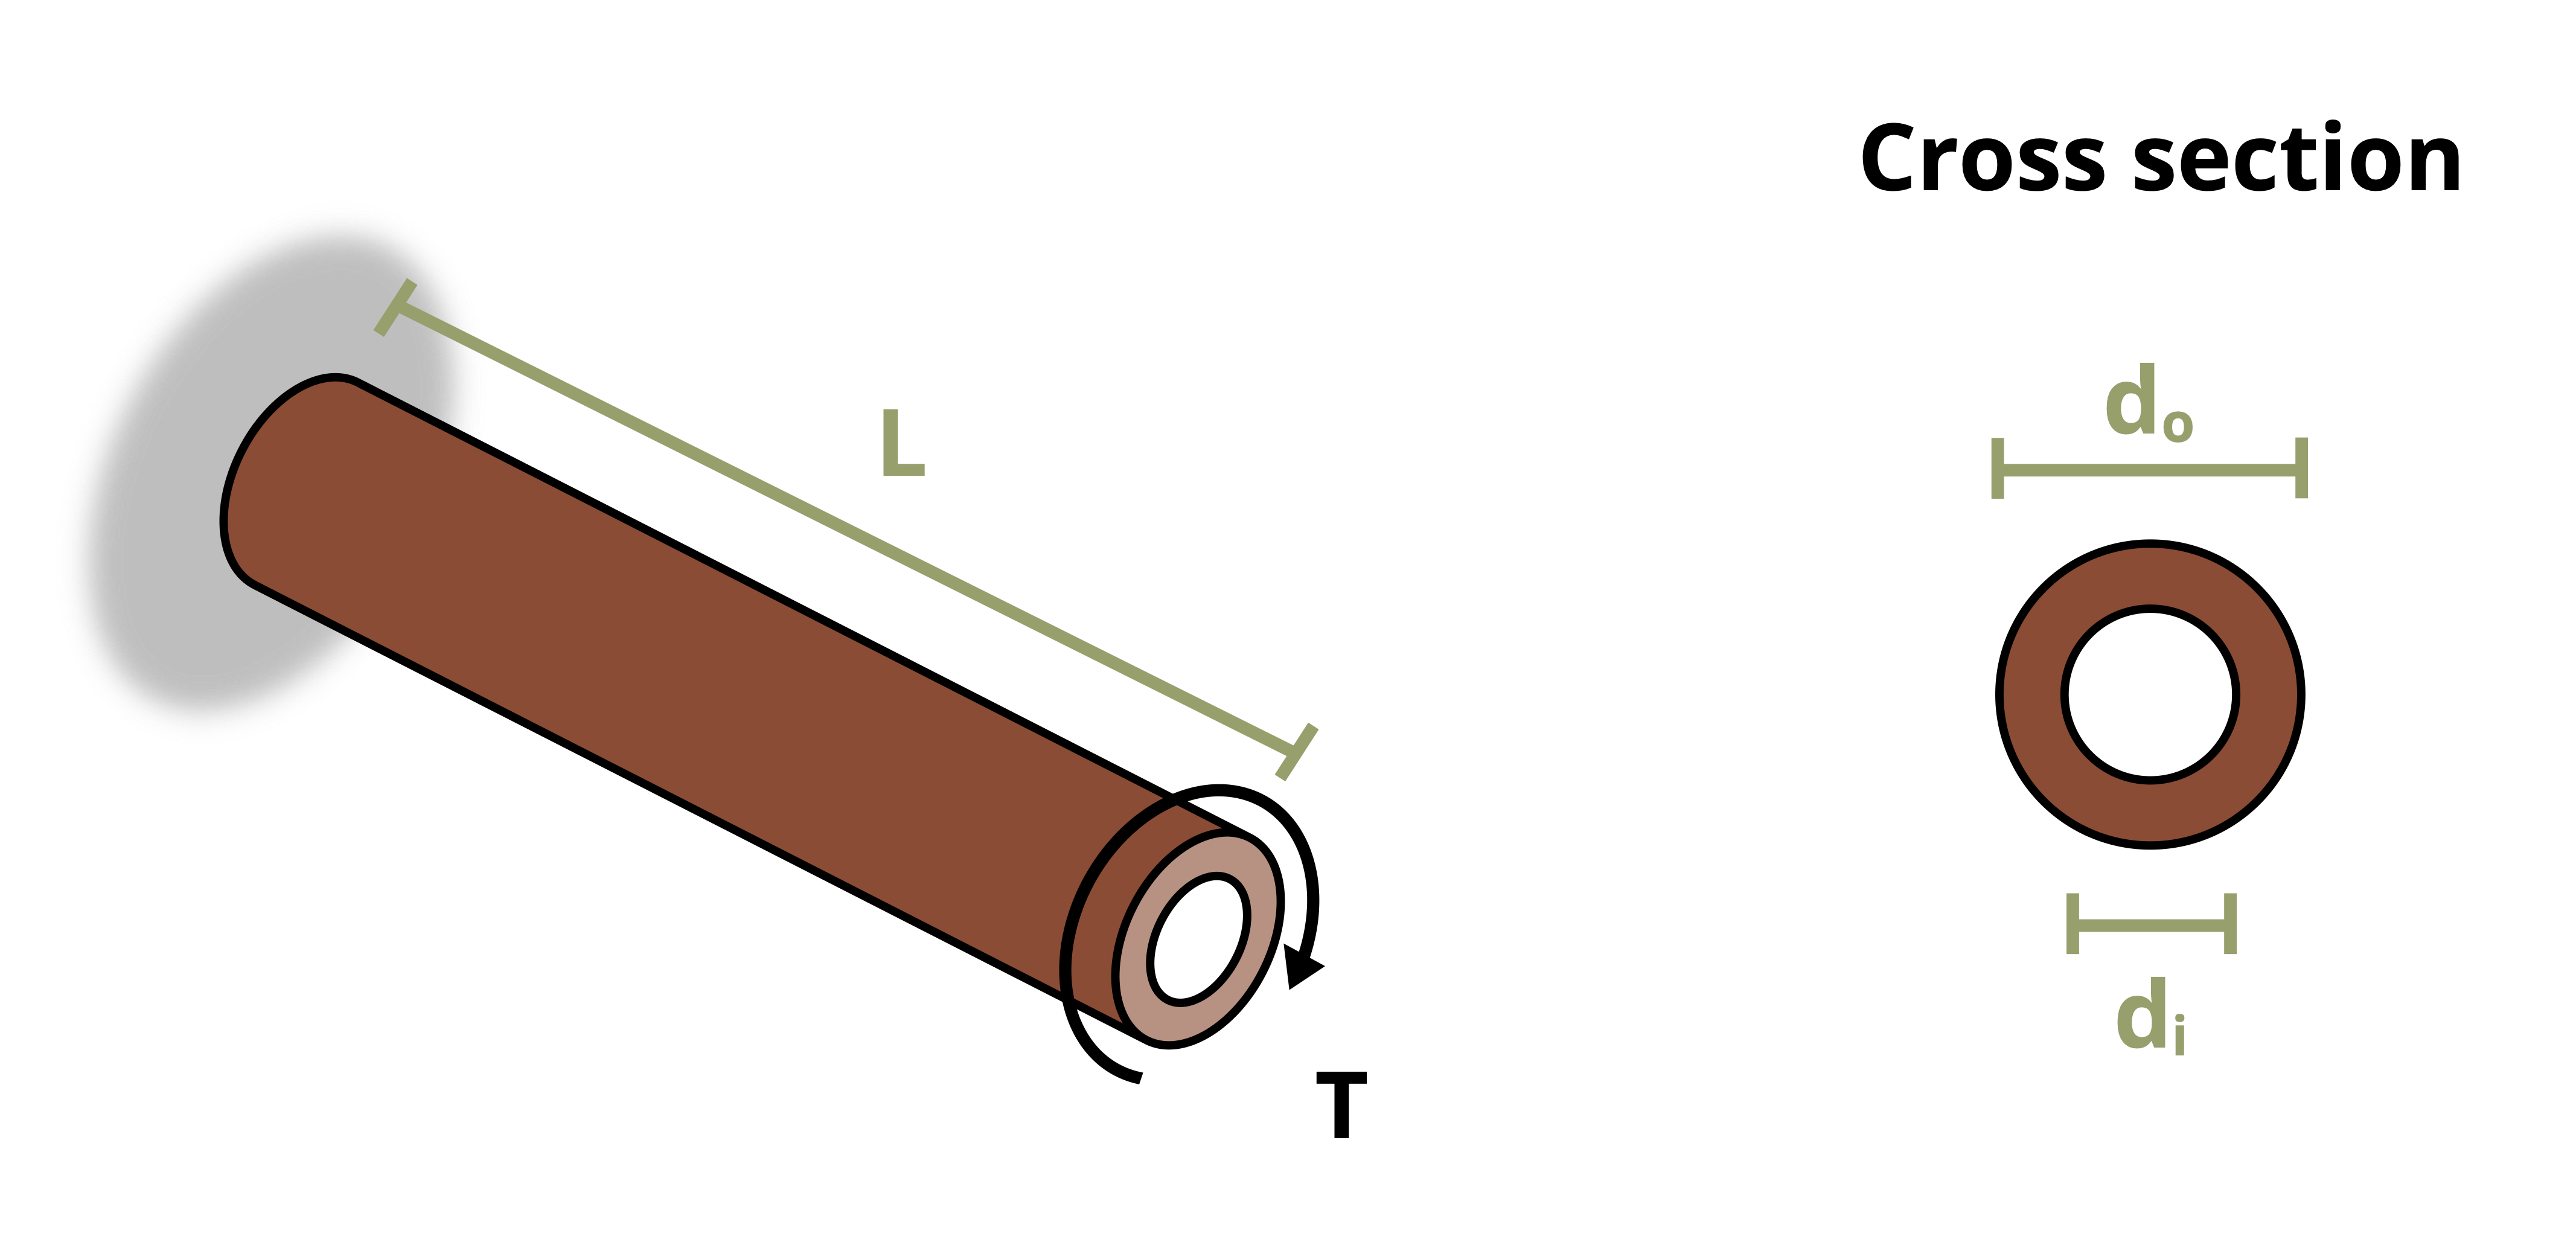
\includegraphics[keepaspectratio]{images/266.png}}

}

\caption{Figure 1: A hollow copper rod is fixed to a wall at one end and
a torque is applied}

\end{figure}%

{[}Problem adapted from © Kurt Gramoll CC BY NC-SA 4.0{]}

\begin{Shaded}
\begin{Highlighting}[]
\NormalTok{\#| standalone: true}
\NormalTok{\#| viewerHeight: 600}
\NormalTok{\#| components: [viewer]}

\NormalTok{from shiny import App, render, ui, reactive}
\NormalTok{import random}
\NormalTok{import asyncio}
\NormalTok{import io}
\NormalTok{import math}
\NormalTok{import string}
\NormalTok{from datetime import datetime}
\NormalTok{from pathlib import Path}

\NormalTok{def generate\_random\_letters(length):}
\NormalTok{    \# Generate a random string of letters of specified length}
\NormalTok{    return \textquotesingle{}\textquotesingle{}.join(random.choice(string.ascii\_lowercase) for \_ in range(length)) }

\NormalTok{problem\_ID="266"}
\NormalTok{L=reactive.Value("\_\_")}
\NormalTok{do=reactive.Value("\_\_")}
\NormalTok{di=reactive.Value("\_\_")}
\NormalTok{angle=(reactive.Value("\_\_"))}
\NormalTok{E = 110}
\NormalTok{v = 0.33}


\NormalTok{attempts=["Timestamp,Attempt,Answer,Feedback\textbackslash{}n"]}

\NormalTok{app\_ui = ui.page\_fluid(}
\NormalTok{    ui.markdown("**Please enter your ID number from your instructor and click to generate your problem**"),}
\NormalTok{    ui.input\_text("ID","", placeholder="Enter ID Number Here"),}
\NormalTok{    ui.input\_action\_button("generate\_problem", "Generate Problem", class\_="btn{-}primary"),}
\NormalTok{    ui.markdown("**Problem Statement**"),}
\NormalTok{    ui.output\_ui("ui\_problem\_statement"),}
\NormalTok{    ui.input\_text("answer","Your Answer in units of kN{-}m", placeholder="Please enter your answer"),}
\NormalTok{    ui.input\_action\_button("submit", "Submit Answer", class\_="btn{-}primary"),}
\NormalTok{    ui.download\_button("download", "Download File to Submit", class\_="btn{-}success"),}
\NormalTok{)}


\NormalTok{def server(input, output, session):}
\NormalTok{    \# Initialize a counter for attempts}
\NormalTok{    attempt\_counter = reactive.Value(0)}

\NormalTok{    @output}
\NormalTok{    @render.ui}
\NormalTok{    def ui\_problem\_statement():}
\NormalTok{        return[ui.markdown(f"A hollow copper rod (E = 110 GPa, v = 0.33) is subjected to torque T as shown. If length L = \{L()\} m, outer diameter d\textless{}sub\textgreater{}o\textless{}/sub\textgreater{} = \{do()\} mm, and inner diameter d\textless{}sub\textgreater{}i\textless{}/sub\textgreater{} = \{di()\} mm, determine torque T if the rod twists \{angle()\}° .")]}
    
\NormalTok{    @reactive.Effect}
\NormalTok{    @reactive.event(input.generate\_problem)}
\NormalTok{    def randomize\_vars():}
\NormalTok{        random.seed(input.ID())}
\NormalTok{        L.set(random.randrange(5, 30, 1)/10)}
\NormalTok{        do.set(random.randrange(50, 200, 1))}
\NormalTok{        di.set(round(do()/2, 2))}
\NormalTok{        angle.set(random.randrange(1, 10, 1))}
        
\NormalTok{    @reactive.Effect}
\NormalTok{    @reactive.event(input.submit)}
\NormalTok{    def \_():}
\NormalTok{        attempt\_counter.set(attempt\_counter() + 1)  \# Increment the attempt counter on each submission.}
\NormalTok{        G = E*10**9/(2*(1+v))}
\NormalTok{        J = (math.pi/2)*((do()/2000)**4 {-}(di()/2000)**4 )}
\NormalTok{        instr= ((math.radians(angle())*G*J)/L())/10**3}
\NormalTok{        if math.isclose(float(input.answer()), instr, rel\_tol=0.01):}
\NormalTok{            check = "*Correct*"}
\NormalTok{            correct\_indicator = "JL"}
\NormalTok{        else:}
\NormalTok{            check = "*Not Correct.*"}
\NormalTok{            correct\_indicator = "JG"}

\NormalTok{        \# Generate random parts for the encoded attempt.}
\NormalTok{        random\_start = generate\_random\_letters(4)}
\NormalTok{        random\_middle = generate\_random\_letters(4)}
\NormalTok{        random\_end = generate\_random\_letters(4)}
\NormalTok{        encoded\_attempt = f"\{random\_start\}\{problem\_ID\}{-}\{random\_middle\}\{attempt\_counter()\}\{correct\_indicator\}{-}\{random\_end\}\{input.ID()\}"}

\NormalTok{        \# Store the most recent encoded attempt in a reactive value so it persists across submissions}
\NormalTok{        session.encoded\_attempt = reactive.Value(encoded\_attempt)}

\NormalTok{        \# Append the attempt data to the attempts list without the encoded attempt}
\NormalTok{        attempts.append(f"\{datetime.now()\}, \{attempt\_counter()\}, \{input.answer()\}, \{check\}\textbackslash{}n")}

\NormalTok{        \# Show feedback to the user.}
\NormalTok{        feedback = ui.markdown(f"Your answer of \{input.answer()\} is \{check\}.")}
\NormalTok{        m = ui.modal(}
\NormalTok{            feedback,}
\NormalTok{            title="Feedback",}
\NormalTok{            easy\_close=True}
\NormalTok{        )}
\NormalTok{        ui.modal\_show(m)}

\NormalTok{    @session.download(filename=lambda: f"Problem\_Log{-}\{problem\_ID\}{-}\{input.ID()\}.csv")}
\NormalTok{    async def download():}
\NormalTok{        \# Start the CSV with the encoded attempt (without label)}
\NormalTok{        final\_encoded = session.encoded\_attempt() if session.encoded\_attempt is not None else "No attempts"}
\NormalTok{        yield f"\{final\_encoded\}\textbackslash{}n\textbackslash{}n"}
        
\NormalTok{        \# Write the header for the remaining CSV data once}
\NormalTok{        yield "Timestamp,Attempt,Answer,Feedback\textbackslash{}n"}
        
\NormalTok{        \# Write the attempts data, ensure that the header from the attempts list is not written again}
\NormalTok{        for attempt in attempts[1:]:  \# Skip the first element which is the header}
\NormalTok{            await asyncio.sleep(0.25)  \# This delay may not be necessary; adjust as needed}
\NormalTok{            yield attempt}


\NormalTok{\# App installation}
\NormalTok{app = App(app\_ui, server)}
\end{Highlighting}
\end{Shaded}

\chapter*{Problem 6.12 - Torsional
Deformation}\label{problem-6.12---torsional-deformation}
\addcontentsline{toc}{chapter}{Problem 6.12 - Torsional Deformation}

\markboth{Problem 6.12 - Torsional Deformation}{Problem 6.12 - Torsional
Deformation}

\begin{figure}[H]

{\centering \pandocbounded{\includegraphics[keepaspectratio]{images/268.png}}

}

\caption{Figure 1: A bar is attached to a wall.}

\end{figure}%

{[}Problem adapted from © Kurt Gramoll CC BY NC-SA 4.0{]}

\begin{Shaded}
\begin{Highlighting}[]
\NormalTok{\#| standalone: true}
\NormalTok{\#| viewerHeight: 600}
\NormalTok{\#| components: [viewer]}

\NormalTok{from shiny import App, render, ui, reactive}
\NormalTok{import random}
\NormalTok{import asyncio}
\NormalTok{import io}
\NormalTok{import math}
\NormalTok{import string}
\NormalTok{from datetime import datetime}
\NormalTok{from pathlib import Path}

\NormalTok{def generate\_random\_letters(length):}
\NormalTok{    \# Generate a random string of letters of specified length}
\NormalTok{    return \textquotesingle{}\textquotesingle{}.join(random.choice(string.ascii\_lowercase) for \_ in range(length)) }

\NormalTok{problem\_ID="268"}
\NormalTok{T1=reactive.Value("\_\_")}
\NormalTok{angle=reactive.Value("\_\_")}
\NormalTok{G=reactive.Value("\_\_")}

\NormalTok{attempts=["Timestamp,Attempt,Answer,Feedback\textbackslash{}n"]}

\NormalTok{app\_ui = ui.page\_fluid(}
\NormalTok{    ui.markdown("**Please enter your ID number from your instructor and click to generate your problem**"),}
\NormalTok{    ui.input\_text("ID","", placeholder="Enter ID Number Here"),}
\NormalTok{    ui.input\_action\_button("generate\_problem", "Generate Problem", class\_="btn{-}primary"),}
\NormalTok{    ui.markdown("**Problem Statement**"),}
\NormalTok{    ui.output\_ui("ui\_problem\_statement"),}
\NormalTok{    ui.input\_text("answer","Your Answer in units of ft{-}lb", placeholder="Please enter your answer"),}
\NormalTok{    ui.input\_action\_button("submit", "Submit Answer", class\_="btn{-}primary"),}
\NormalTok{    ui.download\_button("download", "Download File to Submit", class\_="btn{-}success"),}
\NormalTok{)}


\NormalTok{def server(input, output, session):}
\NormalTok{    \# Initialize a counter for attempts}
\NormalTok{    attempt\_counter = reactive.Value(0)}

\NormalTok{    @output}
\NormalTok{    @render.ui}
\NormalTok{    def ui\_problem\_statement():}
\NormalTok{        return[ui.markdown(f"A bar with a shear modulus G = \{G()\} x 10\textless{}sup\textgreater{}6\textless{}/sup\textgreater{} psi is subjected to torques T\textless{}sub\textgreater{}1\textless{}/sub\textgreater{} = \{T1()\} lb{-}ft at its center and T\textless{}sub\textgreater{}2\textless{}/sub\textgreater{} at its free end. The inner diamter is 1 in and the outer diameter is 2 in and the total length of the bar is 10 in. If the rotation of the rod at its free end is θ =  \{angle()\}° clockwise, what is the magnitude of torque T\textless{}sub\textgreater{}2\textless{}/sub\textgreater{}?")]}
    
\NormalTok{    @reactive.Effect}
\NormalTok{    @reactive.event(input.generate\_problem)}
\NormalTok{    def randomize\_vars():}
\NormalTok{        random.seed(input.ID())}
\NormalTok{        G.set(random.randrange(90, 130, 1)/10)}
\NormalTok{        T1.set(random.randrange(1000, 5000, 100))}
\NormalTok{        angle.set(random.randrange(10, 50, 1)/10)}
        
\NormalTok{    @reactive.Effect}
\NormalTok{    @reactive.event(input.submit)}
\NormalTok{    def \_():}
\NormalTok{        attempt\_counter.set(attempt\_counter() + 1)  \# Increment the attempt counter on each submission.}
\NormalTok{        ro = 2/2}
\NormalTok{        ri = 1/2}
\NormalTok{        J = math.pi/2*(ro**4{-}ri**4)}
\NormalTok{        L1 = 10/2}
\NormalTok{        L2 = 10/2}
\NormalTok{        instr= abs((angle()*math.pi/180*G()*10**6*J+T1()*12*L1)/(L1+L2)/12)}
\NormalTok{        if math.isclose(float(input.answer()), instr, rel\_tol=0.01):}
\NormalTok{            check = "*Correct*"}
\NormalTok{            correct\_indicator = "JL"}
\NormalTok{        else:}
\NormalTok{            check = "*Not Correct.*"}
\NormalTok{            correct\_indicator = "JG"}

\NormalTok{        \# Generate random parts for the encoded attempt.}
\NormalTok{        random\_start = generate\_random\_letters(4)}
\NormalTok{        random\_middle = generate\_random\_letters(4)}
\NormalTok{        random\_end = generate\_random\_letters(4)}
\NormalTok{        encoded\_attempt = f"\{random\_start\}\{problem\_ID\}{-}\{random\_middle\}\{attempt\_counter()\}\{correct\_indicator\}{-}\{random\_end\}\{input.ID()\}"}

\NormalTok{        \# Store the most recent encoded attempt in a reactive value so it persists across submissions}
\NormalTok{        session.encoded\_attempt = reactive.Value(encoded\_attempt)}

\NormalTok{        \# Append the attempt data to the attempts list without the encoded attempt}
\NormalTok{        attempts.append(f"\{datetime.now()\}, \{attempt\_counter()\}, \{input.answer()\}, \{check\}\textbackslash{}n")}

\NormalTok{        \# Show feedback to the user.}
\NormalTok{        feedback = ui.markdown(f"Your answer of \{input.answer()\} is \{check\}.")}
\NormalTok{        m = ui.modal(}
\NormalTok{            feedback,}
\NormalTok{            title="Feedback",}
\NormalTok{            easy\_close=True}
\NormalTok{        )}
\NormalTok{        ui.modal\_show(m)}

\NormalTok{    @session.download(filename=lambda: f"Problem\_Log{-}\{problem\_ID\}{-}\{input.ID()\}.csv")}
\NormalTok{    async def download():}
\NormalTok{        \# Start the CSV with the encoded attempt (without label)}
\NormalTok{        final\_encoded = session.encoded\_attempt() if session.encoded\_attempt is not None else "No attempts"}
\NormalTok{        yield f"\{final\_encoded\}\textbackslash{}n\textbackslash{}n"}
        
\NormalTok{        \# Write the header for the remaining CSV data once}
\NormalTok{        yield "Timestamp,Attempt,Answer,Feedback\textbackslash{}n"}
        
\NormalTok{        \# Write the attempts data, ensure that the header from the attempts list is not written again}
\NormalTok{        for attempt in attempts[1:]:  \# Skip the first element which is the header}
\NormalTok{            await asyncio.sleep(0.25)  \# This delay may not be necessary; adjust as needed}
\NormalTok{            yield attempt}

\NormalTok{\# App installation}
\NormalTok{app = App(app\_ui, server)}
\end{Highlighting}
\end{Shaded}

\chapter*{Problem 6.13 - Torsional
Deformation}\label{problem-6.13---torsional-deformation}
\addcontentsline{toc}{chapter}{Problem 6.13 - Torsional Deformation}

\markboth{Problem 6.13 - Torsional Deformation}{Problem 6.13 - Torsional
Deformation}

\pandocbounded{\includegraphics[keepaspectratio]{images/269.png}}
{[}Problem adapted from © Kurt Gramoll CC BY NC-SA 4.0{]}

\begin{Shaded}
\begin{Highlighting}[]
\NormalTok{\#| standalone: true}
\NormalTok{\#| viewerHeight: 600}
\NormalTok{\#| components: [viewer]}

\NormalTok{from shiny import App, render, ui, reactive}
\NormalTok{import random}
\NormalTok{import asyncio}
\NormalTok{import io}
\NormalTok{import math}
\NormalTok{import string}
\NormalTok{from datetime import datetime}
\NormalTok{from pathlib import Path}

\NormalTok{def generate\_random\_letters(length):}
\NormalTok{    \# Generate a random string of letters of specified length}
\NormalTok{    return \textquotesingle{}\textquotesingle{}.join(random.choice(string.ascii\_lowercase) for \_ in range(length)) }

\NormalTok{problem\_ID="269"}
\NormalTok{T1=reactive.Value("\_\_")}
\NormalTok{T2=reactive.Value("\_\_")}
\NormalTok{T3=reactive.Value("\_\_")}
\NormalTok{Gs=77}
\NormalTok{Ga=27}

\NormalTok{attempts=["Timestamp,Attempt,Answer,Feedback\textbackslash{}n"]}

\NormalTok{app\_ui = ui.page\_fluid(}
\NormalTok{    ui.markdown("**Please enter your ID number from your instructor and click to generate your problem**"),}
\NormalTok{    ui.input\_text("ID","", placeholder="Enter ID Number Here"),}
\NormalTok{    ui.input\_action\_button("generate\_problem", "Generate Problem", class\_="btn{-}primary"),}
\NormalTok{    ui.markdown("**Problem Statement**"),}
\NormalTok{    ui.output\_ui("ui\_problem\_statement"),}
\NormalTok{    ui.input\_text("answer","Your Answer in units of degrees", placeholder="Please enter your answer"),}
\NormalTok{    ui.input\_action\_button("submit", "Submit Answer", class\_="btn{-}primary"),}
\NormalTok{    ui.download\_button("download", "Download File to Submit", class\_="btn{-}success"),}
\NormalTok{)}


\NormalTok{def server(input, output, session):}
\NormalTok{    \# Initialize a counter for attempts}
\NormalTok{    attempt\_counter = reactive.Value(0)}

\NormalTok{    @output}
\NormalTok{    @render.ui}
\NormalTok{    def ui\_problem\_statement():}
\NormalTok{        return[ui.markdown(f"Three moments are applied to the system of cylinders as shown. Assume T\textless{}sub\textgreater{}1\textless{}/sub\textgreater{} = \{T1()\} kN{-}m, T\textless{}sub\textgreater{}2\textless{}/sub\textgreater{} = \{T2()\} kN{-}m, and T\textless{}sub\textgreater{}3\textless{}/sub\textgreater{} = \{T3()\} kN{-}m. If G\textless{}sub\textgreater{}steel\textless{}/sub\textgreater{} = 77 GPa and G\textless{}sub\textgreater{}aluminum\textless{}/sub\textgreater{} = 27 GPa, determine the total angle of twist at the free end.")]}
    
\NormalTok{    @reactive.Effect}
\NormalTok{    @reactive.event(input.generate\_problem)}
\NormalTok{    def randomize\_vars():}
\NormalTok{        random.seed(input.ID())}
\NormalTok{        T1.set(random.randrange(20, 100, 1)/10)}
\NormalTok{        T2.set(T1()+random.randrange(20, 100, 1)/10)}
\NormalTok{        T3.set(round(T2()*random.randrange(5, 8, 1)/10, 2))}
        
\NormalTok{    @reactive.Effect}
\NormalTok{    @reactive.event(input.submit)}
\NormalTok{    def \_():}
\NormalTok{        attempt\_counter.set(attempt\_counter() + 1)  \# Increment the attempt counter on each submission.}
\NormalTok{        F1 = T1()+T2(){-}T3()}
\NormalTok{        F2 = T2(){-}T3()}
\NormalTok{        F3 = {-}T3()}
\NormalTok{        J1 = (math.pi/2)*((5/200)**4)}
\NormalTok{        J2 = (math.pi/2)*((3/200)**4)}
\NormalTok{        J3 = (math.pi/2)*((4/200)**4)}
\NormalTok{        instr= ((F1*1000*.1)/(J1*Gs*10**9) + (F2*1000*.15)/(J2*Ga*10**9) + (F3*1000*.08)/(J3*Gs*10**9))*180/math.pi}
\NormalTok{        if math.isclose(float(input.answer()), instr, rel\_tol=0.01):}
\NormalTok{            check = "*Correct*"}
\NormalTok{            correct\_indicator = "JL"}
\NormalTok{        else:}
\NormalTok{            check = "*Not Correct.*"}
\NormalTok{            correct\_indicator = "JG"}

\NormalTok{        \# Generate random parts for the encoded attempt.}
\NormalTok{        random\_start = generate\_random\_letters(4)}
\NormalTok{        random\_middle = generate\_random\_letters(4)}
\NormalTok{        random\_end = generate\_random\_letters(4)}
\NormalTok{        encoded\_attempt = f"\{random\_start\}\{problem\_ID\}{-}\{random\_middle\}\{attempt\_counter()\}\{correct\_indicator\}{-}\{random\_end\}\{input.ID()\}"}

\NormalTok{        \# Store the most recent encoded attempt in a reactive value so it persists across submissions}
\NormalTok{        session.encoded\_attempt = reactive.Value(encoded\_attempt)}

\NormalTok{        \# Append the attempt data to the attempts list without the encoded attempt}
\NormalTok{        attempts.append(f"\{datetime.now()\}, \{attempt\_counter()\}, \{input.answer()\}, \{check\}\textbackslash{}n")}

\NormalTok{        \# Show feedback to the user.}
\NormalTok{        feedback = ui.markdown(f"Your answer of \{input.answer()\} is \{check\}.")}
\NormalTok{        m = ui.modal(}
\NormalTok{            feedback,}
\NormalTok{            title="Feedback",}
\NormalTok{            easy\_close=True}
\NormalTok{        )}
\NormalTok{        ui.modal\_show(m)}

\NormalTok{    @session.download(filename=lambda: f"Problem\_Log{-}\{problem\_ID\}{-}\{input.ID()\}.csv")}
\NormalTok{    async def download():}
\NormalTok{        \# Start the CSV with the encoded attempt (without label)}
\NormalTok{        final\_encoded = session.encoded\_attempt() if session.encoded\_attempt is not None else "No attempts"}
\NormalTok{        yield f"\{final\_encoded\}\textbackslash{}n\textbackslash{}n"}
        
\NormalTok{        \# Write the header for the remaining CSV data once}
\NormalTok{        yield "Timestamp,Attempt,Answer,Feedback\textbackslash{}n"}
        
\NormalTok{        \# Write the attempts data, ensure that the header from the attempts list is not written again}
\NormalTok{        for attempt in attempts[1:]:  \# Skip the first element which is the header}
\NormalTok{            await asyncio.sleep(0.25)  \# This delay may not be necessary; adjust as needed}
\NormalTok{            yield attempt}

\NormalTok{\# App installation}
\NormalTok{app = App(app\_ui, server)}
\end{Highlighting}
\end{Shaded}

\chapter*{Problem 6.14 - Torsional
Deformation}\label{problem-6.14---torsional-deformation}
\addcontentsline{toc}{chapter}{Problem 6.14 - Torsional Deformation}

\markboth{Problem 6.14 - Torsional Deformation}{Problem 6.14 - Torsional
Deformation}

\pandocbounded{\includegraphics[keepaspectratio]{images/270.png}}
{[}Problem adapted from © Kurt Gramoll CC BY NC-SA 4.0{]}

\begin{Shaded}
\begin{Highlighting}[]
\NormalTok{\#| standalone: true}
\NormalTok{\#| viewerHeight: 600}
\NormalTok{\#| components: [viewer]}

\NormalTok{from shiny import App, render, ui, reactive}
\NormalTok{import random}
\NormalTok{import asyncio}
\NormalTok{import io}
\NormalTok{import math}
\NormalTok{import string}
\NormalTok{from datetime import datetime}
\NormalTok{from pathlib import Path}

\NormalTok{def generate\_random\_letters(length):}
\NormalTok{    \# Generate a random string of letters of specified length}
\NormalTok{    return \textquotesingle{}\textquotesingle{}.join(random.choice(string.ascii\_lowercase) for \_ in range(length)) }

\NormalTok{problem\_ID="270"}
\NormalTok{L=reactive.Value("\_\_")}
\NormalTok{ro=reactive.Value("\_\_")}
\NormalTok{T=reactive.Value("\_\_")}
\NormalTok{G=reactive.Value("\_\_")}
\NormalTok{stress=reactive.Value("\_\_")}

\NormalTok{attempts=["Timestamp,Attempt,Answer,Feedback\textbackslash{}n"]}

\NormalTok{app\_ui = ui.page\_fluid(}
\NormalTok{    ui.markdown("**Please enter your ID number from your instructor and click to generate your problem**"),}
\NormalTok{    ui.input\_text("ID","", placeholder="Enter ID Number Here"),}
\NormalTok{    ui.input\_action\_button("generate\_problem", "Generate Problem", class\_="btn{-}primary"),}
\NormalTok{    ui.markdown("**Problem Statement**"),}
\NormalTok{    ui.output\_ui("ui\_problem\_statement"),}
\NormalTok{    ui.input\_text("answer","Your Answer in units of mm", placeholder="Please enter your answer"),}
\NormalTok{    ui.input\_action\_button("submit", "Submit Answer", class\_="btn{-}primary"),}
\NormalTok{    ui.download\_button("download", "Download File to Submit", class\_="btn{-}success"),}
\NormalTok{)}

\NormalTok{def server(input, output, session):}
\NormalTok{    \# Initialize a counter for attempts}
\NormalTok{    attempt\_counter = reactive.Value(0)}

\NormalTok{    @output}
\NormalTok{    @render.ui}
\NormalTok{    def ui\_problem\_statement():}
\NormalTok{        return[ui.markdown(f"A circular rod of length L = \{L()\} mm, outer radius r\textless{}sub\textgreater{}o\textless{}/sub\textgreater{} = \{ro()\} mm, and unknown inner radius r\textless{}sub\textgreater{}i\textless{}/sub\textgreater{} has a shear modulus G = \{G()\} GPa. The rod is subjected to torque T = \{T()\} kN{-}m at the free end. If the angle of twist must not exceed 2° and the shear stress must not exceed \{stress()\} MPa, what is the minimum required inner radius?")]}
    
\NormalTok{    @reactive.Effect}
\NormalTok{    @reactive.event(input.generate\_problem)}
\NormalTok{    def randomize\_vars():}
\NormalTok{        random.seed(input.ID())}
\NormalTok{        L.set(random.randrange(250, 500, 10))}
\NormalTok{        ro.set(random.randrange(55, 75, 1))}
\NormalTok{        G.set(random.randrange(60, 100, 1))}
\NormalTok{        T.set(random.randrange(10, 100, 1)/10)}
\NormalTok{        stress.set(random.randrange(75, 150, 1))}
        
\NormalTok{    @reactive.Effect}
\NormalTok{    @reactive.event(input.submit)}
\NormalTok{    def \_():}
\NormalTok{        attempt\_counter.set(attempt\_counter() + 1)  \# Increment the attempt counter on each submission.}
\NormalTok{        r1= ((ro()/1000)**4{-}(2*T()*1000*ro()/1000/(math.pi*stress()*10**6)))**0.25*1000}
\NormalTok{        r2 = ((ro()/1000)**4{-}(2*T()*1000*L()/1000/(math.pi*G()*10**9*2*math.pi/180)))**0.25*1000}
\NormalTok{        if r1\textgreater{}r2:}
\NormalTok{            instr = r2}
\NormalTok{        else:}
\NormalTok{            instr = r1}
\NormalTok{        if math.isclose(float(input.answer()), instr, rel\_tol=0.01):}
\NormalTok{            check = "*Correct*"}
\NormalTok{            correct\_indicator = "JL"}
\NormalTok{        else:}
\NormalTok{            check = "*Not Correct.*"}
\NormalTok{            correct\_indicator = "JG"}

\NormalTok{        \# Generate random parts for the encoded attempt.}
\NormalTok{        random\_start = generate\_random\_letters(4)}
\NormalTok{        random\_middle = generate\_random\_letters(4)}
\NormalTok{        random\_end = generate\_random\_letters(4)}
\NormalTok{        encoded\_attempt = f"\{random\_start\}\{problem\_ID\}{-}\{random\_middle\}\{attempt\_counter()\}\{correct\_indicator\}{-}\{random\_end\}\{input.ID()\}"}

\NormalTok{        \# Store the most recent encoded attempt in a reactive value so it persists across submissions}
\NormalTok{        session.encoded\_attempt = reactive.Value(encoded\_attempt)}

\NormalTok{        \# Append the attempt data to the attempts list without the encoded attempt}
\NormalTok{        attempts.append(f"\{datetime.now()\}, \{attempt\_counter()\}, \{input.answer()\}, \{check\}\textbackslash{}n")}

\NormalTok{        \# Show feedback to the user.}
\NormalTok{        feedback = ui.markdown(f"Your answer of \{input.answer()\} is \{check\}.")}
\NormalTok{        m = ui.modal(}
\NormalTok{            feedback,}
\NormalTok{            title="Feedback",}
\NormalTok{            easy\_close=True}
\NormalTok{        )}
\NormalTok{        ui.modal\_show(m)}

\NormalTok{    @session.download(filename=lambda: f"Problem\_Log{-}\{problem\_ID\}{-}\{input.ID()\}.csv")}
\NormalTok{    async def download():}
\NormalTok{        \# Start the CSV with the encoded attempt (without label)}
\NormalTok{        final\_encoded = session.encoded\_attempt() if session.encoded\_attempt is not None else "No attempts"}
\NormalTok{        yield f"\{final\_encoded\}\textbackslash{}n\textbackslash{}n"}
        
\NormalTok{        \# Write the header for the remaining CSV data once}
\NormalTok{        yield "Timestamp,Attempt,Answer,Feedback\textbackslash{}n"}
        
\NormalTok{        \# Write the attempts data, ensure that the header from the attempts list is not written again}
\NormalTok{        for attempt in attempts[1:]:  \# Skip the first element which is the header}
\NormalTok{            await asyncio.sleep(0.25)  \# This delay may not be necessary; adjust as needed}
\NormalTok{            yield attempt}

\NormalTok{\# App installation}
\NormalTok{app = App(app\_ui, server)}
\end{Highlighting}
\end{Shaded}

\chapter*{Problem 6.15 - Torsional
Deformation}\label{problem-6.15---torsional-deformation}
\addcontentsline{toc}{chapter}{Problem 6.15 - Torsional Deformation}

\markboth{Problem 6.15 - Torsional Deformation}{Problem 6.15 - Torsional
Deformation}

\begin{figure}[H]

{\centering \pandocbounded{\includegraphics[keepaspectratio]{images/274.png}}

}

\caption{Figure 1: A hollow circualr rod is attached to a wall and
subjected to a torque at the free end.}

\end{figure}%

{[}Problem adapted from © Kurt Gramoll CC BY NC-SA 4.0{]}

\begin{Shaded}
\begin{Highlighting}[]
\NormalTok{\#| standalone: true}
\NormalTok{\#| viewerHeight: 600}
\NormalTok{\#| components: [viewer]}

\NormalTok{from shiny import App, render, ui, reactive}
\NormalTok{import random}
\NormalTok{import asyncio}
\NormalTok{import io}
\NormalTok{import math}
\NormalTok{import string}
\NormalTok{from datetime import datetime}
\NormalTok{from pathlib import Path}

\NormalTok{def generate\_random\_letters(length):}
\NormalTok{    \# Generate a random string of letters of specified length}
\NormalTok{    return \textquotesingle{}\textquotesingle{}.join(random.choice(string.ascii\_lowercase) for \_ in range(length)) }

\NormalTok{problem\_ID="274"}
\NormalTok{T=reactive.Value("\_\_")}
\NormalTok{x=reactive.Value("\_\_")}
\NormalTok{G=reactive.Value("\_\_")}
\NormalTok{L=reactive.Value("\_\_")}

\NormalTok{attempts=["Timestamp,Attempt,Answer,Feedback\textbackslash{}n"]}

\NormalTok{app\_ui = ui.page\_fluid(}
\NormalTok{    ui.markdown("**Please enter your ID number from your instructor and click to generate your problem**"),}
\NormalTok{    ui.input\_text("ID","", placeholder="Enter ID Number Here"),}
\NormalTok{    ui.input\_action\_button("generate\_problem", "Generate Problem", class\_="btn{-}primary"),}
\NormalTok{    ui.markdown("**Problem Statement**"),}
\NormalTok{    ui.output\_ui("ui\_problem\_statement"),}
\NormalTok{    ui.input\_text("answer","Your Answer in units of degrees", placeholder="Please enter your answer"),}
\NormalTok{    ui.input\_action\_button("submit", "Submit Answer", class\_="btn{-}primary"),}
\NormalTok{    ui.download\_button("download", "Download File to Submit", class\_="btn{-}success"),}
\NormalTok{)}

\NormalTok{def server(input, output, session):}
\NormalTok{    \# Initialize a counter for attempts}
\NormalTok{    attempt\_counter = reactive.Value(0)}

\NormalTok{    @output}
\NormalTok{    @render.ui}
\NormalTok{    def ui\_problem\_statement():}
\NormalTok{        return[ui.markdown(f"A hollow circular rod is attached to a wall and subjected to a torque T = \{T()\} kN{-}m at the free end.The rod has inner diameter 8 cm and outer diameter 10 cm.  Determine the angle of twist at x = \{x()\} mm. Assume G = \{G()\} GPa and L = \{L()\} mm.")]}
    
\NormalTok{    @reactive.Effect}
\NormalTok{    @reactive.event(input.generate\_problem)}
\NormalTok{    def randomize\_vars():}
\NormalTok{        random.seed(input.ID())}
\NormalTok{        T.set(random.randrange(20, 200, 1)/10)}
\NormalTok{        G.set(random.randrange(30, 60, 1))}
\NormalTok{        L.set(random.randrange(300, 800, 10))}
\NormalTok{        x.set(L()*random.randrange(2,7,1)/10)}
        
\NormalTok{    @reactive.Effect}
\NormalTok{    @reactive.event(input.submit)}
\NormalTok{    def \_():}
\NormalTok{        attempt\_counter.set(attempt\_counter() + 1)  \# Increment the attempt counter on each submission.}
\NormalTok{        J = (math.pi/2)*((10/200)**4 {-} (8/200)**4)}
\NormalTok{        angle = (T()*1000*x()/1000)/(G()*10**9*J)}
\NormalTok{        instr= math.degrees(angle)}
\NormalTok{        if math.isclose(float(input.answer()), instr, rel\_tol=0.01):}
\NormalTok{            check = "*Correct*"}
\NormalTok{            correct\_indicator = "JL"}
\NormalTok{        else:}
\NormalTok{            check = "*Not Correct.*"}
\NormalTok{            correct\_indicator = "JG"}

\NormalTok{        \# Generate random parts for the encoded attempt.}
\NormalTok{        random\_start = generate\_random\_letters(4)}
\NormalTok{        random\_middle = generate\_random\_letters(4)}
\NormalTok{        random\_end = generate\_random\_letters(4)}
\NormalTok{        encoded\_attempt = f"\{random\_start\}\{problem\_ID\}{-}\{random\_middle\}\{attempt\_counter()\}\{correct\_indicator\}{-}\{random\_end\}\{input.ID()\}"}

\NormalTok{        \# Store the most recent encoded attempt in a reactive value so it persists across submissions}
\NormalTok{        session.encoded\_attempt = reactive.Value(encoded\_attempt)}

\NormalTok{        \# Append the attempt data to the attempts list without the encoded attempt}
\NormalTok{        attempts.append(f"\{datetime.now()\}, \{attempt\_counter()\}, \{input.answer()\}, \{check\}\textbackslash{}n")}

\NormalTok{        \# Show feedback to the user.}
\NormalTok{        feedback = ui.markdown(f"Your answer of \{input.answer()\} is \{check\}.")}
\NormalTok{        m = ui.modal(}
\NormalTok{            feedback,}
\NormalTok{            title="Feedback",}
\NormalTok{            easy\_close=True}
\NormalTok{        )}
\NormalTok{        ui.modal\_show(m)}

\NormalTok{    @session.download(filename=lambda: f"Problem\_Log{-}\{problem\_ID\}{-}\{input.ID()\}.csv")}
\NormalTok{    async def download():}
\NormalTok{        \# Start the CSV with the encoded attempt (without label)}
\NormalTok{        final\_encoded = session.encoded\_attempt() if session.encoded\_attempt is not None else "No attempts"}
\NormalTok{        yield f"\{final\_encoded\}\textbackslash{}n\textbackslash{}n"}
        
\NormalTok{        \# Write the header for the remaining CSV data once}
\NormalTok{        yield "Timestamp,Attempt,Answer,Feedback\textbackslash{}n"}
        
\NormalTok{        \# Write the attempts data, ensure that the header from the attempts list is not written again}
\NormalTok{        for attempt in attempts[1:]:  \# Skip the first element which is the header}
\NormalTok{            await asyncio.sleep(0.25)  \# This delay may not be necessary; adjust as needed}
\NormalTok{            yield attempt}

\NormalTok{\# App installation}
\NormalTok{app = App(app\_ui, server)}
\end{Highlighting}
\end{Shaded}

\chapter*{Problem 6.22 - Power Transmission \& Gear
Assemblies}\label{problem-6.22---power-transmission-gear-assemblies}
\addcontentsline{toc}{chapter}{Problem 6.22 - Power Transmission \& Gear
Assemblies}

\markboth{Problem 6.22 - Power Transmission \& Gear Assemblies}{Problem
6.22 - Power Transmission \& Gear Assemblies}

\pandocbounded{\includegraphics[keepaspectratio]{images/669.png}}
{[}Problem adapted from © Chris Galitz CC BY NC-SA 4.0{]}

\begin{Shaded}
\begin{Highlighting}[]
\NormalTok{\#| standalone: true}
\NormalTok{\#| viewerHeight: 600}
\NormalTok{\#| components: [viewer]}

\NormalTok{from shiny import App, render, ui, reactive}
\NormalTok{import random}
\NormalTok{import asyncio}
\NormalTok{import io}
\NormalTok{import math}
\NormalTok{import string}
\NormalTok{from datetime import datetime}
\NormalTok{from pathlib import Path}

\NormalTok{def generate\_random\_letters(length):}
\NormalTok{    \# Generate a random string of letters of specified length}
\NormalTok{    return \textquotesingle{}\textquotesingle{}.join(random.choice(string.ascii\_lowercase) for \_ in range(length))  }

\NormalTok{problem\_ID="669"}
\NormalTok{P=reactive.Value("\_\_")}
\NormalTok{rpm=reactive.Value("\_\_")}
\NormalTok{T=reactive.Value("\_\_")}

\NormalTok{attempts=["Timestamp,Attempt,Answer,Feedback\textbackslash{}n"]}

\NormalTok{app\_ui = ui.page\_fluid(}
\NormalTok{    ui.markdown("**Please enter your ID number from your instructor and click to generate your problem**"),}
\NormalTok{    ui.input\_text("ID","", placeholder="Enter ID Number Here"),}
\NormalTok{    ui.input\_action\_button("generate\_problem", "Generate Problem", class\_="btn{-}primary"),}
\NormalTok{    ui.markdown("**Problem Statement**"),}
\NormalTok{    ui.output\_ui("ui\_problem\_statement"),}
\NormalTok{    ui.input\_text("answer","Your Answer in units of N*m", placeholder="Please enter your answer"),}
\NormalTok{    ui.input\_action\_button("submit", "Submit Answer", class\_="btn{-}primary"),}
\NormalTok{    ui.download\_button("download", "Download File to Submit", class\_="btn{-}success"),}
\NormalTok{)}

\NormalTok{def server(input, output, session):}
\NormalTok{    \# Initialize a counter for attempts}
\NormalTok{    attempt\_counter = reactive.Value(0)}

\NormalTok{    @output}
\NormalTok{    @render.ui}
\NormalTok{    def ui\_problem\_statement():}
\NormalTok{        return[ui.markdown(f"The steel shaft is being turned by an electric motor providing \{P()\} kW of power at \{rpm()\} rpm. Power is extracted at B with a torque of \{T()\} N⸱m. Determine the remaining torque available for the gear at C.")]}
    
\NormalTok{    @reactive.Effect}
\NormalTok{    @reactive.event(input.generate\_problem)}
\NormalTok{    def randomize\_vars():}
\NormalTok{        random.seed(input.ID())}
\NormalTok{        P.set(random.randrange(10, 30, 1))}
\NormalTok{        rpm.set(random.randrange(60, 180, 5))}
\NormalTok{        T.set(random.randrange(200, 400, 10))}
        
\NormalTok{    @reactive.Effect}
\NormalTok{    @reactive.event(input.submit)}
\NormalTok{    def \_():}
\NormalTok{        attempt\_counter.set(attempt\_counter() + 1)  \# Increment the attempt counter on each submission.}
\NormalTok{        TA = P()*1000/(2*math.pi*rpm()/60)}
\NormalTok{        instr= TA{-}T()}
\NormalTok{        if math.isclose(float(input.answer()), instr, rel\_tol=0.01):}
\NormalTok{            check = "*Correct*"}
\NormalTok{            correct\_indicator = "JL"}
\NormalTok{        else:}
\NormalTok{            check = "*Not Correct.*"}
\NormalTok{            correct\_indicator = "JG"}

\NormalTok{        \# Generate random parts for the encoded attempt.}
\NormalTok{        random\_start = generate\_random\_letters(4)}
\NormalTok{        random\_middle = generate\_random\_letters(4)}
\NormalTok{        random\_end = generate\_random\_letters(4)}
\NormalTok{        encoded\_attempt = f"\{random\_start\}\{problem\_ID\}{-}\{random\_middle\}\{attempt\_counter()\}\{correct\_indicator\}{-}\{random\_end\}\{input.ID()\}"}

\NormalTok{        \# Store the most recent encoded attempt in a reactive value so it persists across submissions}
\NormalTok{        session.encoded\_attempt = reactive.Value(encoded\_attempt)}

\NormalTok{        \# Append the attempt data to the attempts list without the encoded attempt}
\NormalTok{        attempts.append(f"\{datetime.now()\}, \{attempt\_counter()\}, \{input.answer()\}, \{check\}\textbackslash{}n")}

\NormalTok{        \# Show feedback to the user.}
\NormalTok{        feedback = ui.markdown(f"Your answer of \{input.answer()\} is \{check\}.")}
\NormalTok{        m = ui.modal(}
\NormalTok{            feedback,}
\NormalTok{            title="Feedback",}
\NormalTok{            easy\_close=True}
\NormalTok{        )}
\NormalTok{        ui.modal\_show(m)}

\NormalTok{    @session.download(filename=lambda: f"Problem\_Log{-}\{problem\_ID\}{-}\{input.ID()\}.csv")}
\NormalTok{    async def download():}
\NormalTok{        \# Start the CSV with the encoded attempt (without label)}
\NormalTok{        final\_encoded = session.encoded\_attempt() if session.encoded\_attempt is not None else "No attempts"}
\NormalTok{        yield f"\{final\_encoded\}\textbackslash{}n\textbackslash{}n"}
        
\NormalTok{        \# Write the header for the remaining CSV data once}
\NormalTok{        yield "Timestamp,Attempt,Answer,Feedback\textbackslash{}n"}
        
\NormalTok{        \# Write the attempts data, ensure that the header from the attempts list is not written again}
\NormalTok{        for attempt in attempts[1:]:  \# Skip the first element which is the header}
\NormalTok{            await asyncio.sleep(0.25)  \# This delay may not be necessary; adjust as needed}
\NormalTok{            yield attempt}

\NormalTok{\# App installation}
\NormalTok{app = App(app\_ui, server)}
\end{Highlighting}
\end{Shaded}

\chapter*{Problem 6.23 - Power Transmission \& Gear
Assemblies}\label{problem-6.23---power-transmission-gear-assemblies}
\addcontentsline{toc}{chapter}{Problem 6.23 - Power Transmission \& Gear
Assemblies}

\markboth{Problem 6.23 - Power Transmission \& Gear Assemblies}{Problem
6.23 - Power Transmission \& Gear Assemblies}

\includegraphics[width=3.125in,height=\textheight,keepaspectratio]{images/670.png}
{[}Problem adapted from © Chris Galitz CC BY NC-SA 4.0{]}

\begin{Shaded}
\begin{Highlighting}[]
\NormalTok{\#| standalone: true}
\NormalTok{\#| viewerHeight: 600}
\NormalTok{\#| components: [viewer]}

\NormalTok{from shiny import App, render, ui, reactive}
\NormalTok{import random}
\NormalTok{import asyncio}
\NormalTok{import io}
\NormalTok{import math}
\NormalTok{import string}
\NormalTok{from datetime import datetime}
\NormalTok{from pathlib import Path}

\NormalTok{def generate\_random\_letters(length):}
\NormalTok{    \# Generate a random string of letters of specified length}
\NormalTok{    return \textquotesingle{}\textquotesingle{}.join(random.choice(string.ascii\_lowercase) for \_ in range(length))  }

\NormalTok{problem\_ID="670"}
\NormalTok{hp=reactive.Value("\_\_")}
\NormalTok{rpm=reactive.Value("\_\_")}

\NormalTok{attempts=["Timestamp,Attempt,Answer,Feedback\textbackslash{}n"]}

\NormalTok{app\_ui = ui.page\_fluid(}
\NormalTok{    ui.markdown("**Please enter your ID number from your instructor and click to generate your problem**"),}
\NormalTok{    ui.input\_text("ID","", placeholder="Enter ID Number Here"),}
\NormalTok{    ui.input\_action\_button("generate\_problem", "Generate Problem", class\_="btn{-}primary"),}
\NormalTok{    ui.markdown("**Problem Statement**"),}
\NormalTok{    ui.output\_ui("ui\_problem\_statement"),}
\NormalTok{    ui.input\_text("answer","Your Answer in units of lb", placeholder="Please enter your answer"),}
\NormalTok{    ui.input\_action\_button("submit", "Submit Answer", class\_="btn{-}primary"),}
\NormalTok{    ui.download\_button("download", "Download File to Submit", class\_="btn{-}success"),}
\NormalTok{)}

\NormalTok{def server(input, output, session):}
\NormalTok{    \# Initialize a counter for attempts}
\NormalTok{    attempt\_counter = reactive.Value(0)}

\NormalTok{    @output}
\NormalTok{    @render.ui}
\NormalTok{    def ui\_problem\_statement():}
\NormalTok{        return[ui.markdown(f"A lawnmower engine supplying \{hp()\} hp running at \{rpm()\} rpm is being used to power a homemade winch. Given the gearing shown, determine the heaviest load that can be lifted.")]}
    
\NormalTok{    @reactive.Effect}
\NormalTok{    @reactive.event(input.generate\_problem)}
\NormalTok{    def randomize\_vars():}
\NormalTok{        random.seed(input.ID())}
\NormalTok{        hp.set(random.randrange(10, 50, 1)/10)}
\NormalTok{        rpm.set(random.randrange(2000, 4000, 100))}
        
\NormalTok{    @reactive.Effect}
\NormalTok{    @reactive.event(input.submit)}
\NormalTok{    def \_():}
\NormalTok{        attempt\_counter.set(attempt\_counter() + 1)  \# Increment the attempt counter on each submission.}
\NormalTok{        T = hp()*550/(2*math.pi*rpm()/60)*12}
\NormalTok{        instr= T/0.5}
\NormalTok{        if math.isclose(float(input.answer()), instr, rel\_tol=0.01):}
\NormalTok{            check = "*Correct*"}
\NormalTok{            correct\_indicator = "JL"}
\NormalTok{        else:}
\NormalTok{            check = "*Not Correct.*"}
\NormalTok{            correct\_indicator = "JG"}

\NormalTok{        \# Generate random parts for the encoded attempt.}
\NormalTok{        random\_start = generate\_random\_letters(4)}
\NormalTok{        random\_middle = generate\_random\_letters(4)}
\NormalTok{        random\_end = generate\_random\_letters(4)}
\NormalTok{        encoded\_attempt = f"\{random\_start\}\{problem\_ID\}{-}\{random\_middle\}\{attempt\_counter()\}\{correct\_indicator\}{-}\{random\_end\}\{input.ID()\}"}

\NormalTok{        \# Store the most recent encoded attempt in a reactive value so it persists across submissions}
\NormalTok{        session.encoded\_attempt = reactive.Value(encoded\_attempt)}

\NormalTok{        \# Append the attempt data to the attempts list without the encoded attempt}
\NormalTok{        attempts.append(f"\{datetime.now()\}, \{attempt\_counter()\}, \{input.answer()\}, \{check\}\textbackslash{}n")}

\NormalTok{        \# Show feedback to the user.}
\NormalTok{        feedback = ui.markdown(f"Your answer of \{input.answer()\} is \{check\}.")}
\NormalTok{        m = ui.modal(}
\NormalTok{            feedback,}
\NormalTok{            title="Feedback",}
\NormalTok{            easy\_close=True}
\NormalTok{        )}
\NormalTok{        ui.modal\_show(m)}

\NormalTok{    @session.download(filename=lambda: f"Problem\_Log{-}\{problem\_ID\}{-}\{input.ID()\}.csv")}
\NormalTok{    async def download():}
\NormalTok{        \# Start the CSV with the encoded attempt (without label)}
\NormalTok{        final\_encoded = session.encoded\_attempt() if session.encoded\_attempt is not None else "No attempts"}
\NormalTok{        yield f"\{final\_encoded\}\textbackslash{}n\textbackslash{}n"}
        
\NormalTok{        \# Write the header for the remaining CSV data once}
\NormalTok{        yield "Timestamp,Attempt,Answer,Feedback\textbackslash{}n"}
        
\NormalTok{        \# Write the attempts data, ensure that the header from the attempts list is not written again}
\NormalTok{        for attempt in attempts[1:]:  \# Skip the first element which is the header}
\NormalTok{            await asyncio.sleep(0.25)  \# This delay may not be necessary; adjust as needed}
\NormalTok{            yield attempt}

\NormalTok{\# App installation}
\NormalTok{app = App(app\_ui, server)}
\end{Highlighting}
\end{Shaded}

\chapter*{Problem 6.27 - Statically Indeterminate
Torsion}\label{problem-6.27---statically-indeterminate-torsion}
\addcontentsline{toc}{chapter}{Problem 6.27 - Statically Indeterminate
Torsion}

\markboth{Problem 6.27 - Statically Indeterminate Torsion}{Problem 6.27
- Statically Indeterminate Torsion}

\pandocbounded{\includegraphics[keepaspectratio]{images/287.png}}
{[}Problem adapted from © Kurt Gramoll CC BY NC-SA 4.0{]}

\begin{Shaded}
\begin{Highlighting}[]
\NormalTok{\#| standalone: true}
\NormalTok{\#| viewerHeight: 600}
\NormalTok{\#| components: [viewer]}

\NormalTok{from shiny import App, render, ui, reactive}
\NormalTok{import random}
\NormalTok{import asyncio}
\NormalTok{import io}
\NormalTok{import math}
\NormalTok{import string}
\NormalTok{from datetime import datetime}
\NormalTok{from pathlib import Path}

\NormalTok{def generate\_random\_letters(length):}
\NormalTok{    \# Generate a random string of letters of specified length}
\NormalTok{    return \textquotesingle{}\textquotesingle{}.join(random.choice(string.ascii\_lowercase) for \_ in range(length)) }

\NormalTok{problem\_ID="287"}
\NormalTok{L=reactive.Value("\_\_")}
\NormalTok{F=reactive.Value("\_\_")}
\NormalTok{d=reactive.Value("\_\_")}
\NormalTok{G = 75}

\NormalTok{attempts=["Timestamp,Attempt,Answer,Feedback\textbackslash{}n"]}

\NormalTok{app\_ui = ui.page\_fluid(}
\NormalTok{    ui.markdown("**Please enter your ID number from your instructor and click to generate your problem**"),}
\NormalTok{    ui.input\_text("ID","", placeholder="Enter ID Number Here"),}
\NormalTok{    ui.input\_action\_button("generate\_problem", "Generate Problem", class\_="btn{-}primary"),}
\NormalTok{    ui.markdown("**Problem Statement**"),}
\NormalTok{    ui.output\_ui("ui\_problem\_statement"),}
\NormalTok{    ui.input\_text("answer","Your Answer in units of MPa", placeholder="Please enter your answer"),}
\NormalTok{    ui.input\_action\_button("submit", "Submit Answer", class\_="btn{-}primary"),}
\NormalTok{    ui.download\_button("download", "Download File to Submit", class\_="btn{-}success"),}
\NormalTok{)}


\NormalTok{def server(input, output, session):}
\NormalTok{    \# Initialize a counter for attempts}
\NormalTok{    attempt\_counter = reactive.Value(0)}

\NormalTok{    @output}
\NormalTok{    @render.ui}
\NormalTok{    def ui\_problem\_statement():}
\NormalTok{        return[ui.markdown(f"A steel rod of diameter d = \{d()\} mm is attached to walls A and C as shown. Two forces F = \{F()\} kN are applied at distance L = \{L()\} mm. If the shear modulus of the rod G = 75 GPa, determine the maximum shear stress in the rod.")]}
    
\NormalTok{    @reactive.Effect}
\NormalTok{    @reactive.event(input.generate\_problem)}
\NormalTok{    def randomize\_vars():}
\NormalTok{        random.seed(input.ID())}
\NormalTok{        d.set(random.randrange(20, 60, 1))}
\NormalTok{        F.set(random.randrange(2, 20, 1))}
\NormalTok{        L.set(random.randrange(80, 120, 1))}
        
        
\NormalTok{    @reactive.Effect}
\NormalTok{    @reactive.event(input.submit)}
\NormalTok{    def \_():}
\NormalTok{        attempt\_counter.set(attempt\_counter() + 1)  \# Increment the attempt counter on each submission.}
\NormalTok{        TB = 2*F()*L()}
\NormalTok{        J = (math.pi/2)*(d()/2000)**4}
\NormalTok{        TA = 0.3/0.7*TB}
\NormalTok{        TC = TB{-}TA}
\NormalTok{        instr= ((TC*(d()/2000))/J)/10**6}
\NormalTok{        if math.isclose(float(input.answer()), instr, rel\_tol=0.01):}
\NormalTok{            check = "*Correct*"}
\NormalTok{            correct\_indicator = "JL"}
\NormalTok{        else:}
\NormalTok{            check = "*Not Correct.*"}
\NormalTok{            correct\_indicator = "JG"}

\NormalTok{        \# Generate random parts for the encoded attempt.}
\NormalTok{        random\_start = generate\_random\_letters(4)}
\NormalTok{        random\_middle = generate\_random\_letters(4)}
\NormalTok{        random\_end = generate\_random\_letters(4)}
\NormalTok{        encoded\_attempt = f"\{random\_start\}\{problem\_ID\}{-}\{random\_middle\}\{attempt\_counter()\}\{correct\_indicator\}{-}\{random\_end\}\{input.ID()\}"}

\NormalTok{        \# Store the most recent encoded attempt in a reactive value so it persists across submissions}
\NormalTok{        session.encoded\_attempt = reactive.Value(encoded\_attempt)}

\NormalTok{        \# Append the attempt data to the attempts list without the encoded attempt}
\NormalTok{        attempts.append(f"\{datetime.now()\}, \{attempt\_counter()\}, \{input.answer()\}, \{check\}\textbackslash{}n")}

\NormalTok{        \# Show feedback to the user.}
\NormalTok{        feedback = ui.markdown(f"Your answer of \{input.answer()\} is \{check\}.")}
\NormalTok{        m = ui.modal(}
\NormalTok{            feedback,}
\NormalTok{            title="Feedback",}
\NormalTok{            easy\_close=True}
\NormalTok{        )}
\NormalTok{        ui.modal\_show(m)}

\NormalTok{    @session.download(filename=lambda: f"Problem\_Log{-}\{problem\_ID\}{-}\{input.ID()\}.csv")}
\NormalTok{    async def download():}
\NormalTok{        \# Start the CSV with the encoded attempt (without label)}
\NormalTok{        final\_encoded = session.encoded\_attempt() if session.encoded\_attempt is not None else "No attempts"}
\NormalTok{        yield f"\{final\_encoded\}\textbackslash{}n\textbackslash{}n"}
        
\NormalTok{        \# Write the header for the remaining CSV data once}
\NormalTok{        yield "Timestamp,Attempt,Answer,Feedback\textbackslash{}n"}
        
\NormalTok{        \# Write the attempts data, ensure that the header from the attempts list is not written again}
\NormalTok{        for attempt in attempts[1:]:  \# Skip the first element which is the header}
\NormalTok{            await asyncio.sleep(0.25)  \# This delay may not be necessary; adjust as needed}
\NormalTok{            yield attempt}


\NormalTok{\# App installation}
\NormalTok{app = App(app\_ui, server)}
\end{Highlighting}
\end{Shaded}

\chapter*{Problem 6.28 - Statically Indeterminate
Torsion}\label{problem-6.28---statically-indeterminate-torsion}
\addcontentsline{toc}{chapter}{Problem 6.28 - Statically Indeterminate
Torsion}

\markboth{Problem 6.28 - Statically Indeterminate Torsion}{Problem 6.28
- Statically Indeterminate Torsion}

\pandocbounded{\includegraphics[keepaspectratio]{images/288.png}}
{[}Problem adapted from © Kurt Gramoll CC BY NC-SA 4.0{]}

\begin{Shaded}
\begin{Highlighting}[]
\NormalTok{\#| standalone: true}
\NormalTok{\#| viewerHeight: 600}
\NormalTok{\#| components: [viewer]}

\NormalTok{from shiny import App, render, ui, reactive}
\NormalTok{import random}
\NormalTok{import asyncio}
\NormalTok{import io}
\NormalTok{import math}
\NormalTok{import string}
\NormalTok{from datetime import datetime}
\NormalTok{from pathlib import Path}

\NormalTok{def generate\_random\_letters(length):}
\NormalTok{    \# Generate a random string of letters of specified length}
\NormalTok{    return \textquotesingle{}\textquotesingle{}.join(random.choice(string.ascii\_lowercase) for \_ in range(length)) }

\NormalTok{problem\_ID="288"}
\NormalTok{T=reactive.Value("\_\_")}
\NormalTok{L=reactive.Value("\_\_")}
\NormalTok{G1=reactive.Value("\_\_")}
\NormalTok{G2=reactive.Value("\_\_")}

\NormalTok{attempts=["Timestamp,Attempt,Answer,Feedback\textbackslash{}n"]}

\NormalTok{app\_ui = ui.page\_fluid(}
\NormalTok{    ui.markdown("**Please enter your ID number from your instructor and click to generate your problem**"),}
\NormalTok{    ui.input\_text("ID","", placeholder="Enter ID Number Here"),}
\NormalTok{    ui.input\_action\_button("generate\_problem", "Generate Problem", class\_="btn{-}primary"),}
\NormalTok{    ui.markdown("**Problem Statement**"),}
\NormalTok{    ui.output\_ui("ui\_problem\_statement"),}
\NormalTok{    ui.input\_text("answer","Your Answer in units of MPa", placeholder="Please enter your answer"),}
\NormalTok{    ui.input\_action\_button("submit", "Submit Answer", class\_="btn{-}primary"),}
\NormalTok{    ui.download\_button("download", "Download File to Submit", class\_="btn{-}success"),}
\NormalTok{)}

\NormalTok{def server(input, output, session):}
\NormalTok{    \# Initialize a counter for attempts}
\NormalTok{    attempt\_counter = reactive.Value(0)}

\NormalTok{    @output}
\NormalTok{    @render.ui}
\NormalTok{    def ui\_problem\_statement():}
\NormalTok{        return[ui.markdown(f"A composite circular rod is made from two different plastics. A torque of T = \{T()\} kN{-}m is applied at the midpoint. The right end is free. What is the maximum stress in either material? Assume length L = \{L()\} cm and the shear modulus of the two materials are G\textless{}sub\textgreater{}1\textless{}/sub\textgreater{} = \{G1()\} GPa and G\textless{}sub\textgreater{}2\textless{}/sub\textgreater{} = \{G2()\} GPa.")]}
    
\NormalTok{    @reactive.Effect}
\NormalTok{    @reactive.event(input.generate\_problem)}
\NormalTok{    def randomize\_vars():}
\NormalTok{        random.seed(input.ID())}
\NormalTok{        T.set(random.randrange(10, 200, 1)/10)}
\NormalTok{        L.set(random.randrange(10, 50, 1))}
\NormalTok{        G1.set(random.randrange(20, 50, 2)/10)}
\NormalTok{        G2.set(G1()/2)}
        
        
\NormalTok{    @reactive.Effect}
\NormalTok{    @reactive.event(input.submit)}
\NormalTok{    def \_():}
\NormalTok{        attempt\_counter.set(attempt\_counter() + 1)  \# Increment the attempt counter on each submission.}
\NormalTok{        J1 = (math.pi/2)*(2/100)**4}
\NormalTok{        J2 = (math.pi/2)*((3/100)**4{-}(2/100)**4)}
\NormalTok{        RHS = G1()*10**9*J1+G2()*10**9*J2}
\NormalTok{        LHS = T()*G2()*10**9*J2}
\NormalTok{        T2 = LHS/RHS}
\NormalTok{        T1 = T(){-}T2}
\NormalTok{        instr= ((T1*(2/100))/J1)/1000}
\NormalTok{        if math.isclose(float(input.answer()), instr, rel\_tol=0.01):}
\NormalTok{            check = "*Correct*"}
\NormalTok{            correct\_indicator = "JL"}
\NormalTok{        else:}
\NormalTok{            check = "*Not Correct.*"}
\NormalTok{            correct\_indicator = "JG"}

\NormalTok{        \# Generate random parts for the encoded attempt.}
\NormalTok{        random\_start = generate\_random\_letters(4)}
\NormalTok{        random\_middle = generate\_random\_letters(4)}
\NormalTok{        random\_end = generate\_random\_letters(4)}
\NormalTok{        encoded\_attempt = f"\{random\_start\}\{problem\_ID\}{-}\{random\_middle\}\{attempt\_counter()\}\{correct\_indicator\}{-}\{random\_end\}\{input.ID()\}"}

\NormalTok{        \# Store the most recent encoded attempt in a reactive value so it persists across submissions}
\NormalTok{        session.encoded\_attempt = reactive.Value(encoded\_attempt)}

\NormalTok{        \# Append the attempt data to the attempts list without the encoded attempt}
\NormalTok{        attempts.append(f"\{datetime.now()\}, \{attempt\_counter()\}, \{input.answer()\}, \{check\}\textbackslash{}n")}

\NormalTok{        \# Show feedback to the user.}
\NormalTok{        feedback = ui.markdown(f"Your answer of \{input.answer()\} is \{check\}.")}
\NormalTok{        m = ui.modal(}
\NormalTok{            feedback,}
\NormalTok{            title="Feedback",}
\NormalTok{            easy\_close=True}
\NormalTok{        )}
\NormalTok{        ui.modal\_show(m)}

\NormalTok{    @session.download(filename=lambda: f"Problem\_Log{-}\{problem\_ID\}{-}\{input.ID()\}.csv")}
\NormalTok{    async def download():}
\NormalTok{        \# Start the CSV with the encoded attempt (without label)}
\NormalTok{        final\_encoded = session.encoded\_attempt() if session.encoded\_attempt is not None else "No attempts"}
\NormalTok{        yield f"\{final\_encoded\}\textbackslash{}n\textbackslash{}n"}
        
\NormalTok{        \# Write the header for the remaining CSV data once}
\NormalTok{        yield "Timestamp,Attempt,Answer,Feedback\textbackslash{}n"}
        
\NormalTok{        \# Write the attempts data, ensure that the header from the attempts list is not written again}
\NormalTok{        for attempt in attempts[1:]:  \# Skip the first element which is the header}
\NormalTok{            await asyncio.sleep(0.25)  \# This delay may not be necessary; adjust as needed}
\NormalTok{            yield attempt}

\NormalTok{\# App installation}
\NormalTok{app = App(app\_ui, server)}
\end{Highlighting}
\end{Shaded}

\chapter*{Problem 6.29 - Statically Indeterminate
Torsion}\label{problem-6.29---statically-indeterminate-torsion}
\addcontentsline{toc}{chapter}{Problem 6.29 - Statically Indeterminate
Torsion}

\markboth{Problem 6.29 - Statically Indeterminate Torsion}{Problem 6.29
- Statically Indeterminate Torsion}

\begin{figure}[H]

{\centering \pandocbounded{\includegraphics[keepaspectratio]{images/289.png}}

}

\caption{Figure 1: A composite circular rod is made from aluminum and
steel.}

\end{figure}%

{[}Problem adapted from © Kurt Gramoll CC BY NC-SA 4.0{]}

\begin{Shaded}
\begin{Highlighting}[]
\NormalTok{\#| standalone: true}
\NormalTok{\#| viewerHeight: 600}
\NormalTok{\#| components: [viewer]}

\NormalTok{from shiny import App, render, ui, reactive}
\NormalTok{import random}
\NormalTok{import asyncio}
\NormalTok{import io}
\NormalTok{import math}
\NormalTok{import string}
\NormalTok{from datetime import datetime}
\NormalTok{from pathlib import Path}

\NormalTok{def generate\_random\_letters(length):}
\NormalTok{    \# Generate a random string of letters of specified length}
\NormalTok{    return "".join(random.choice(string.ascii\_lowercase) for \_ in range(length))}

\NormalTok{problem\_ID = "289"}
\NormalTok{T = reactive.Value("\_\_")}
\NormalTok{L = reactive.Value("\_\_")}
\NormalTok{ro = reactive.Value("\_\_")}
\NormalTok{ri = reactive.Value("\_\_")}
\NormalTok{GA = 3800000}
\NormalTok{GS = 11000000}

\NormalTok{attempts = ["Timestamp,Attempt,Answer,Feedback\textbackslash{}n"]}

\NormalTok{app\_ui = ui.page\_fluid(}
\NormalTok{    ui.markdown(}
\NormalTok{        "**Please enter your ID number from your instructor and click to generate your problem**"}
\NormalTok{    ),}
\NormalTok{    ui.input\_text("ID", "", placeholder="Enter ID Number Here"),}
\NormalTok{    ui.input\_action\_button(}
\NormalTok{        "generate\_problem", "Generate Problem", class\_="btn{-}primary"}
\NormalTok{    ),}
\NormalTok{    ui.markdown("**Problem Statement**"),}
\NormalTok{    ui.output\_ui("ui\_problem\_statement"),}
\NormalTok{    ui.input\_text(}
\NormalTok{        "answer", "Your Answer in units of ksi", placeholder="Please enter your answer"}
\NormalTok{    ),}
\NormalTok{    ui.input\_action\_button("submit", "Submit Answer", class\_="btn{-}primary"),}
\NormalTok{    ui.download\_button("download", "Download File to Submit", class\_="btn{-}success"),}
\NormalTok{)}

\NormalTok{def server(input, output, session):}
\NormalTok{    \# Initialize a counter for attempts}
\NormalTok{    attempt\_counter = reactive.Value(0)}

\NormalTok{    @output}
\NormalTok{    @render.ui}
\NormalTok{    def ui\_problem\_statement():}
\NormalTok{        return [}
\NormalTok{            ui.markdown(}
\NormalTok{                f"A composite circular rod is made from aluminum (G = 3,800 ksi) and steel (G = 11,000 ksi) as shown. A torque T = \{T()\} lb{-}ft is applied to the free end. What is the maximum stress in either material? Assume length L = \{L()\} in., outer radius r\textless{}sub\textgreater{}o\textless{}/sub\textgreater{} = \{ro()\} in., and inner radius r\textless{}sub\textgreater{}i\textless{}/sub\textgreater{} = \{ri()\} in."}
\NormalTok{            )}
\NormalTok{        ]}

\NormalTok{    @reactive.Effect}
\NormalTok{    @reactive.event(input.generate\_problem)}
\NormalTok{    def randomize\_vars():}
\NormalTok{        random.seed(input.ID())}
\NormalTok{        T.set(random.randrange(300, 2000, 100))}
\NormalTok{        L.set(random.randrange(10, 60, 1))}
\NormalTok{        ro.set(random.randrange(10, 60, 1) / 10)}
\NormalTok{        ri.set(round(ro() / 1.5, 1))}

\NormalTok{    @reactive.Effect}
\NormalTok{    @reactive.event(input.submit)}
\NormalTok{    def \_():}
\NormalTok{        attempt\_counter.set(}
\NormalTok{            attempt\_counter() + 1}
\NormalTok{        )  \# Increment the attempt counter on each submission.}
\NormalTok{        JS = math.pi * ri() ** 4 / 2}
\NormalTok{        JA = math.pi / 2 * (ro() ** 4 {-} ri() ** 4)}
\NormalTok{        TA = T() * 12 * GA * JA / (GS * JS + GA * JA)}
\NormalTok{        TS = T() * 12 {-} TA}
\NormalTok{        instr = TS * ri() / JS / 1000}
\NormalTok{        if math.isclose(float(input.answer()), instr, rel\_tol=0.01):}
\NormalTok{            check = "*Correct*"}
\NormalTok{            correct\_indicator = "JL"}
\NormalTok{        else:}
\NormalTok{            check = "*Not Correct.*"}
\NormalTok{            correct\_indicator = "JG"}

\NormalTok{        \# Generate random parts for the encoded attempt.}
\NormalTok{        random\_start = generate\_random\_letters(4)}
\NormalTok{        random\_middle = generate\_random\_letters(4)}
\NormalTok{        random\_end = generate\_random\_letters(4)}
\NormalTok{        encoded\_attempt = f"\{random\_start\}\{problem\_ID\}{-}\{random\_middle\}\{attempt\_counter()\}\{correct\_indicator\}{-}\{random\_end\}\{input.ID()\}"}

\NormalTok{        \# Store the most recent encoded attempt in a reactive value so it persists across submissions}
\NormalTok{        session.encoded\_attempt = reactive.Value(encoded\_attempt)}

\NormalTok{        \# Append the attempt data to the attempts list without the encoded attempt}
\NormalTok{        attempts.append(}
\NormalTok{            f"\{datetime.now()\}, \{attempt\_counter()\}, \{input.answer()\}, \{check\}\textbackslash{}n"}
\NormalTok{        )}

\NormalTok{        \# Show feedback to the user.}
\NormalTok{        feedback = ui.markdown(}
\NormalTok{            f"Your answer of \{input.answer()\} is \{check\}.")}
\NormalTok{        m = ui.modal(feedback, title="Feedback", easy\_close=True)}
\NormalTok{        ui.modal\_show(m)}

\NormalTok{    @session.download(filename=lambda: f"Problem\_Log{-}\{problem\_ID\}{-}\{input.ID()\}.csv")}
\NormalTok{    async def download():}
\NormalTok{        \# Start the CSV with the encoded attempt (without label)}
\NormalTok{        final\_encoded = (}
\NormalTok{            session.encoded\_attempt()}
\NormalTok{            if session.encoded\_attempt is not None}
\NormalTok{            else "No attempts"}
\NormalTok{        )}
\NormalTok{        yield f"\{final\_encoded\}\textbackslash{}n\textbackslash{}n"}

\NormalTok{        \# Write the header for the remaining CSV data once}
\NormalTok{        yield "Timestamp,Attempt,Answer,Feedback\textbackslash{}n"}

\NormalTok{        \# Write the attempts data, ensure that the header from the attempts list is not written again}
\NormalTok{        for attempt in attempts[1:]:  \# Skip the first element which is the header}
\NormalTok{            await asyncio.sleep(}
\NormalTok{                0.25}
\NormalTok{            )  \# This delay may not be necessary; adjust as needed}
\NormalTok{            yield attempt}


\NormalTok{\# App installation}
\NormalTok{app = App(app\_ui, server)}
\end{Highlighting}
\end{Shaded}

\chapter*{Problem 6.30 - Statically Indeterminate
Torsion}\label{problem-6.30---statically-indeterminate-torsion}
\addcontentsline{toc}{chapter}{Problem 6.30 - Statically Indeterminate
Torsion}

\markboth{Problem 6.30 - Statically Indeterminate Torsion}{Problem 6.30
- Statically Indeterminate Torsion}

\pandocbounded{\includegraphics[keepaspectratio]{images/292.png}}
{[}Problem adapted from © Kurt Gramoll CC BY NC-SA 4.0{]}

\begin{Shaded}
\begin{Highlighting}[]
\NormalTok{\#| standalone: true}
\NormalTok{\#| viewerHeight: 600}
\NormalTok{\#| components: [viewer]}

\NormalTok{from shiny import App, render, ui, reactive}
\NormalTok{import random}
\NormalTok{import asyncio}
\NormalTok{import io}
\NormalTok{import math}
\NormalTok{import string}
\NormalTok{from datetime import datetime}
\NormalTok{from pathlib import Path}

\NormalTok{def generate\_random\_letters(length):}
\NormalTok{    \# Generate a random string of letters of specified length}
\NormalTok{    return \textquotesingle{}\textquotesingle{}.join(random.choice(string.ascii\_lowercase) for \_ in range(length)) }

\NormalTok{problem\_ID="292"}
\NormalTok{T=reactive.Value("\_\_")}
\NormalTok{d1=reactive.Value("\_\_")}
\NormalTok{d2=reactive.Value("\_\_")}
\NormalTok{L1=reactive.Value("\_\_")}
\NormalTok{L2=reactive.Value("\_\_")}
\NormalTok{Gn = 11.4e6}
\NormalTok{Ga = 4e6}

\NormalTok{attempts=["Timestamp,Attempt,Answer,Feedback\textbackslash{}n"]}

\NormalTok{app\_ui = ui.page\_fluid(}
\NormalTok{    ui.markdown("**Please enter your ID number from your instructor and click to generate your problem**"),}
\NormalTok{    ui.input\_text("ID","", placeholder="Enter ID Number Here"),}
\NormalTok{    ui.input\_action\_button("generate\_problem", "Generate Problem", class\_="btn{-}primary"),}
\NormalTok{    ui.markdown("**Problem Statement**"),}
\NormalTok{    ui.output\_ui("ui\_problem\_statement"),}
\NormalTok{    ui.input\_text("answer","Your Answer in units of psi", placeholder="Please enter your answer"),}
\NormalTok{    ui.input\_action\_button("submit", "Submit Answer", class\_="btn{-}primary"),}
\NormalTok{    ui.download\_button("download", "Download File to Submit", class\_="btn{-}success"),}
\NormalTok{)}


\NormalTok{def server(input, output, session):}
\NormalTok{    \# Initialize a counter for attempts}
\NormalTok{    attempt\_counter = reactive.Value(0)}

\NormalTok{    @output}
\NormalTok{    @render.ui}
\NormalTok{    def ui\_problem\_statement():}
\NormalTok{        return[ui.markdown(f"A shaft is fixed between two walls. One portion is made from nickel (G\textless{}sub\textgreater{}nickel\textless{}/sub\textgreater{} = 11.4 x 10\textless{}sup\textgreater{}6\textless{}/sup\textgreater{} psi) with a diameter of d\textless{}sub\textgreater{}1\textless{}/sub\textgreater{} = \{d1()\} in. The other portion is aluminum (G\textless{}sub\textgreater{}aluminum\textless{}/sub\textgreater{} = 4 x 10\textless{}sup\textgreater{}6\textless{}/sup\textgreater{} psi) with a diameter of d\textless{}sub\textgreater{}2\textless{}/sub\textgreater{} = \{d2()\} in. A torque T = \{T()\} lb{-}ft is applied at the point where the two materials meet. If lengths L\textless{}sub\textgreater{}1\textless{}/sub\textgreater{} = \{L1()\} ft and L\textless{}sub\textgreater{}2\textless{}/sub\textgreater{} = \{L2()\} ft, what is the maximum shear stress in the shaft?")]}
    
\NormalTok{    @reactive.Effect}
\NormalTok{    @reactive.event(input.generate\_problem)}
\NormalTok{    def randomize\_vars():}
\NormalTok{        random.seed(input.ID())}
\NormalTok{        d1.set(random.randrange(10, 60, 1)/10)}
\NormalTok{        d2.set(round(d1()*2, 2))}
\NormalTok{        T.set(random.randrange(500, 2000, 100))}
\NormalTok{        L1.set(random.randrange(4, 20, 2))}
\NormalTok{        L2.set(L1()/2)}
        
\NormalTok{    @reactive.Effect}
\NormalTok{    @reactive.event(input.submit)}
\NormalTok{    def \_():}
\NormalTok{        attempt\_counter.set(attempt\_counter() + 1)  \# Increment the attempt counter on each submission.}
\NormalTok{        Jn = (math.pi/2)*(d1()/2)**4}
\NormalTok{        Ja = (math.pi/2)*(d2()/2)**4}
\NormalTok{        TN = T()*12*L2()*12*Gn*Jn/(L1()*12*Ga*Ja+L2()*12*Gn*Jn)}
\NormalTok{        TA = T()*12{-}TN}
\NormalTok{        tauA = TA*d2()/2/Ja}
\NormalTok{        tauN = TN*d1()/2/Jn}
\NormalTok{        if tauA\textgreater{}=tauN:}
\NormalTok{            instr = tauA}
\NormalTok{        else:}
\NormalTok{            instr = tauN}
\NormalTok{        if math.isclose(float(input.answer()), instr, rel\_tol=0.01):}
\NormalTok{            check = "*Correct*"}
\NormalTok{            correct\_indicator = "JL"}
\NormalTok{        else:}
\NormalTok{            check = "*Not Correct.*"}
\NormalTok{            correct\_indicator = "JG"}

\NormalTok{        \# Generate random parts for the encoded attempt.}
\NormalTok{        random\_start = generate\_random\_letters(4)}
\NormalTok{        random\_middle = generate\_random\_letters(4)}
\NormalTok{        random\_end = generate\_random\_letters(4)}
\NormalTok{        encoded\_attempt = f"\{random\_start\}\{problem\_ID\}{-}\{random\_middle\}\{attempt\_counter()\}\{correct\_indicator\}{-}\{random\_end\}\{input.ID()\}"}

\NormalTok{        \# Store the most recent encoded attempt in a reactive value so it persists across submissions}
\NormalTok{        session.encoded\_attempt = reactive.Value(encoded\_attempt)}

\NormalTok{        \# Append the attempt data to the attempts list without the encoded attempt}
\NormalTok{        attempts.append(f"\{datetime.now()\}, \{attempt\_counter()\}, \{input.answer()\}, \{check\}\textbackslash{}n")}

\NormalTok{        \# Show feedback to the user.}
\NormalTok{        feedback = ui.markdown(f"Your answer of \{input.answer()\} is \{check\}.")}
\NormalTok{        m = ui.modal(}
\NormalTok{            feedback,}
\NormalTok{            title="Feedback",}
\NormalTok{            easy\_close=True}
\NormalTok{        )}
\NormalTok{        ui.modal\_show(m)}

\NormalTok{    @session.download(filename=lambda: f"Problem\_Log{-}\{problem\_ID\}{-}\{input.ID()\}.csv")}
\NormalTok{    async def download():}
\NormalTok{        \# Start the CSV with the encoded attempt (without label)}
\NormalTok{        final\_encoded = session.encoded\_attempt() if session.encoded\_attempt is not None else "No attempts"}
\NormalTok{        yield f"\{final\_encoded\}\textbackslash{}n\textbackslash{}n"}
        
\NormalTok{        \# Write the header for the remaining CSV data once}
\NormalTok{        yield "Timestamp,Attempt,Answer,Feedback\textbackslash{}n"}
        
\NormalTok{        \# Write the attempts data, ensure that the header from the attempts list is not written again}
\NormalTok{        for attempt in attempts[1:]:  \# Skip the first element which is the header}
\NormalTok{            await asyncio.sleep(0.25)  \# This delay may not be necessary; adjust as needed}
\NormalTok{            yield attempt}

\NormalTok{\# App installation}
\NormalTok{app = App(app\_ui, server)}
\end{Highlighting}
\end{Shaded}

\chapter*{Problem 6.31 - Statically Indeterminate
Torsion}\label{problem-6.31---statically-indeterminate-torsion}
\addcontentsline{toc}{chapter}{Problem 6.31 - Statically Indeterminate
Torsion}

\markboth{Problem 6.31 - Statically Indeterminate Torsion}{Problem 6.31
- Statically Indeterminate Torsion}

\pandocbounded{\includegraphics[keepaspectratio]{images/293.png}}
{[}Problem adapted from © Kurt Gramoll CC BY NC-SA 4.0{]}

\begin{Shaded}
\begin{Highlighting}[]
\NormalTok{\#| standalone: true}
\NormalTok{\#| viewerHeight: 600}
\NormalTok{\#| components: [viewer]}

\NormalTok{from shiny import App, render, ui, reactive}
\NormalTok{import random}
\NormalTok{import asyncio}
\NormalTok{import io}
\NormalTok{import math}
\NormalTok{import string}
\NormalTok{from datetime import datetime}
\NormalTok{from pathlib import Path}

\NormalTok{def generate\_random\_letters(length):}
\NormalTok{    \# Generate a random string of letters of specified length}
\NormalTok{    return \textquotesingle{}\textquotesingle{}.join(random.choice(string.ascii\_lowercase) for \_ in range(length)) }

\NormalTok{problem\_ID="293"}
\NormalTok{T=reactive.Value("\_\_")}
\NormalTok{d1=reactive.Value("\_\_")}
\NormalTok{d2=reactive.Value("\_\_")}
\NormalTok{L=reactive.Value("\_\_")}
\NormalTok{G = 80}

\NormalTok{attempts=["Timestamp,Attempt,Answer,Feedback\textbackslash{}n"]}

\NormalTok{app\_ui = ui.page\_fluid(}
\NormalTok{    ui.markdown("**Please enter your ID number from your instructor and click to generate your problem**"),}
\NormalTok{    ui.input\_text("ID","", placeholder="Enter ID Number Here"),}
\NormalTok{    ui.input\_action\_button("generate\_problem", "Generate Problem", class\_="btn{-}primary"),}
\NormalTok{    ui.markdown("**Problem Statement**"),}
\NormalTok{    ui.output\_ui("ui\_problem\_statement"),}
\NormalTok{    ui.input\_text("answer","Your Answer in units of MPa", placeholder="Please enter your answer"),}
\NormalTok{    ui.input\_action\_button("submit", "Submit Answer", class\_="btn{-}primary"),}
\NormalTok{    ui.download\_button("download", "Download File to Submit", class\_="btn{-}success"),}
\NormalTok{)}

\NormalTok{def server(input, output, session):}
\NormalTok{    \# Initialize a counter for attempts}
\NormalTok{    attempt\_counter = reactive.Value(0)}

\NormalTok{    @output}
\NormalTok{    @render.ui}
\NormalTok{    def ui\_problem\_statement():}
\NormalTok{        return[ui.markdown(f"Two steel (G = 80 GPa) circular rods are firmly welded together and attached between two walls. Assume d\textless{}sub\textgreater{}1\textless{}/sub\textgreater{} = \{d1()\} mm, d\textless{}sub\textgreater{}2\textless{}/sub\textgreater{} = \{d2()\} mm, and L  = \{L()\} mm. A torque T = \{T()\} N{-}m is applied at the welded joint as shown. What is the highest stress in either rod?")]}
    
\NormalTok{    @reactive.Effect}
\NormalTok{    @reactive.event(input.generate\_problem)}
\NormalTok{    def randomize\_vars():}
\NormalTok{        random.seed(input.ID())}
\NormalTok{        d1.set(random.randrange(20, 50, 1))}
\NormalTok{        d2.set(round(d1()*.8, 2))}
\NormalTok{        L.set(random.randrange(100, 800, 10))}
\NormalTok{        T.set(random.randrange(10, 300, 5))}
        
\NormalTok{    @reactive.Effect}
\NormalTok{    @reactive.event(input.submit)}
\NormalTok{    def \_():}
\NormalTok{        attempt\_counter.set(attempt\_counter() + 1)  \# Increment the attempt counter on each submission.}
\NormalTok{        J1 = (math.pi/2)*(d1()/2000)**4}
\NormalTok{        J2 = (math.pi/2)*(d2()/2000)**4}
\NormalTok{        RHS = J1/J2}
\NormalTok{        Tb = (T()/(RHS+1))}
\NormalTok{        Ta = T() {-} Tb}
\NormalTok{        tauA = (Ta*d1()/2000/J1)/10**6}
\NormalTok{        tauB = (Tb*d2()/2000/J2)/10**6}
\NormalTok{        if tauA\textgreater{}=tauB:}
\NormalTok{            instr = tauA}
\NormalTok{        else:}
\NormalTok{            instr = tauB}
\NormalTok{        if math.isclose(float(input.answer()), instr, rel\_tol=0.01):}
\NormalTok{            check = "*Correct*"}
\NormalTok{            correct\_indicator = "JL"}
\NormalTok{        else:}
\NormalTok{            check = "*Not Correct.*"}
\NormalTok{            correct\_indicator = "JG"}

\NormalTok{        \# Generate random parts for the encoded attempt.}
\NormalTok{        random\_start = generate\_random\_letters(4)}
\NormalTok{        random\_middle = generate\_random\_letters(4)}
\NormalTok{        random\_end = generate\_random\_letters(4)}
\NormalTok{        encoded\_attempt = f"\{random\_start\}\{problem\_ID\}{-}\{random\_middle\}\{attempt\_counter()\}\{correct\_indicator\}{-}\{random\_end\}\{input.ID()\}"}

\NormalTok{        \# Store the most recent encoded attempt in a reactive value so it persists across submissions}
\NormalTok{        session.encoded\_attempt = reactive.Value(encoded\_attempt)}

\NormalTok{        \# Append the attempt data to the attempts list without the encoded attempt}
\NormalTok{        attempts.append(f"\{datetime.now()\}, \{attempt\_counter()\}, \{input.answer()\}, \{check\}\textbackslash{}n")}

\NormalTok{        \# Show feedback to the user.}
\NormalTok{        feedback = ui.markdown(f"Your answer of \{input.answer()\} is \{check\}.")}
\NormalTok{        m = ui.modal(}
\NormalTok{            feedback,}
\NormalTok{            title="Feedback",}
\NormalTok{            easy\_close=True}
\NormalTok{        )}
\NormalTok{        ui.modal\_show(m)}

\NormalTok{    @session.download(filename=lambda: f"Problem\_Log{-}\{problem\_ID\}{-}\{input.ID()\}.csv")}
\NormalTok{    async def download():}
\NormalTok{        \# Start the CSV with the encoded attempt (without label)}
\NormalTok{        final\_encoded = session.encoded\_attempt() if session.encoded\_attempt is not None else "No attempts"}
\NormalTok{        yield f"\{final\_encoded\}\textbackslash{}n\textbackslash{}n"}
        
\NormalTok{        \# Write the header for the remaining CSV data once}
\NormalTok{        yield "Timestamp,Attempt,Answer,Feedback\textbackslash{}n"}
        
\NormalTok{        \# Write the attempts data, ensure that the header from the attempts list is not written again}
\NormalTok{        for attempt in attempts[1:]:  \# Skip the first element which is the header}
\NormalTok{            await asyncio.sleep(0.25)  \# This delay may not be necessary; adjust as needed}
\NormalTok{            yield attempt}

\NormalTok{\# App installation}
\NormalTok{app = App(app\_ui, server)}
\end{Highlighting}
\end{Shaded}

\part{Chapter 7 Problems}

\chapter*{Problem 7.1 - Internal Shear Force \& Bending Moment by
Equilibrium}\label{problem-7.1---internal-shear-force-bending-moment-by-equilibrium}
\addcontentsline{toc}{chapter}{Problem 7.1 - Internal Shear Force \&
Bending Moment by Equilibrium}

\markboth{Problem 7.1 - Internal Shear Force \& Bending Moment by
Equilibrium}{Problem 7.1 - Internal Shear Force \& Bending Moment by
Equilibrium}

\pandocbounded{\includegraphics[keepaspectratio]{images/305.png}}
{[}Problem adapted from © Kurt Gramoll CC BY NC-SA 4.0{]}

\begin{Shaded}
\begin{Highlighting}[]
\NormalTok{\#| standalone: true}
\NormalTok{\#| viewerHeight: 600}
\NormalTok{\#| components: [viewer]}

\NormalTok{from shiny import App, render, ui, reactive}
\NormalTok{import random}
\NormalTok{import asyncio}
\NormalTok{import io}
\NormalTok{import math}
\NormalTok{import string}
\NormalTok{from datetime import datetime}
\NormalTok{from pathlib import Path}

\NormalTok{def generate\_random\_letters(length):}
\NormalTok{    return \textquotesingle{}\textquotesingle{}.join(random.choice(string.ascii\_lowercase) for \_ in range(length))}

\NormalTok{problem\_ID = "305"}
\NormalTok{w = reactive.Value("\_\_")}
\NormalTok{F = reactive.Value("\_\_")}

\NormalTok{attempts = ["Timestamp,Attempt,Answer1,Answer2,Feedback\textbackslash{}n"]}

\NormalTok{app\_ui = ui.page\_fluid(}
\NormalTok{    ui.markdown("**Please enter your ID number from your instructor and click to generate your problem**"),}
\NormalTok{    ui.input\_text("ID", "", placeholder="Enter ID Number Here"),}
\NormalTok{    ui.input\_action\_button("generate\_problem", "Generate Problem", class\_="btn{-}primary"),}
\NormalTok{    ui.markdown("**Problem Statement**"),}
\NormalTok{    ui.output\_ui("ui\_problem\_statement"),}
\NormalTok{    ui.input\_text("answer1", "Your internal shear force answer in units of lb", placeholder="Please enter your answer 1"),}
\NormalTok{    ui.input\_text("answer2", "Your moment answer in units of lb{-}ft", placeholder="Please enter your answer 2"),}
\NormalTok{    ui.input\_action\_button("submit", "Submit Answers", class\_="btn{-}primary"),}
\NormalTok{    ui.download\_button("download", "Download File to Submit", class\_="btn{-}success"),}
\NormalTok{)}

\NormalTok{def server(input, output, session):}
\NormalTok{    attempt\_counter = reactive.Value(0)}

\NormalTok{    @output}
\NormalTok{    @render.ui}
\NormalTok{    def ui\_problem\_statement():}
\NormalTok{        return [ui.markdown(f"A beam is subjected to the loading shown, where w = \{w()\} lb/ft and F = \{F()\} lb. Determine the internal shear force and bending moment at section a{-}a.")]}

\NormalTok{    @reactive.Effect}
\NormalTok{    @reactive.event(input.generate\_problem)}
\NormalTok{    def randomize\_vars():}
\NormalTok{        random.seed(input.ID())}
\NormalTok{        w.set(random.randrange(5, 150, 5))}
\NormalTok{        F.set(random.randrange(300, 750, 10))}

\NormalTok{    @reactive.Effect}
\NormalTok{    @reactive.event(input.submit)}
\NormalTok{    def \_():}
\NormalTok{        attempt\_counter.set(attempt\_counter() + 1)}
\NormalTok{        Ay = (F()*2 {-} w()*6*3) / {-}6}
\NormalTok{        instr1 = Ay {-} w()*3}
\NormalTok{        instr2 = Ay*3 {-} w()*3*1.5}
\NormalTok{        correct1 = math.isclose(float(input.answer1()), instr1, rel\_tol=0.01)}
\NormalTok{        correct2 = math.isclose(float(input.answer2()), instr2, rel\_tol=0.01)}
        
\NormalTok{        if correct1 and correct2:}
\NormalTok{            check = "both correct."}
\NormalTok{        elif correct1:}
\NormalTok{            check = f" \{\textquotesingle{}correct for answer 1 and incorrect for answer 2.\textquotesingle{}\}"}
\NormalTok{        elif correct2:}
\NormalTok{            check = f"\{\textquotesingle{}incorrect for answer 1 and correct for answer 2.\textquotesingle{}\}"}
\NormalTok{        else:}
\NormalTok{            check = f"\{\textquotesingle{}both incorrect.\textquotesingle{}\}"}
        
\NormalTok{        correct\_indicator = "JL" if correct1 and correct2 else "JG"}

\NormalTok{        random\_start = generate\_random\_letters(4)}
\NormalTok{        random\_middle = generate\_random\_letters(4)}
\NormalTok{        random\_end = generate\_random\_letters(4)}
\NormalTok{        encoded\_attempt = f"\{random\_start\}\{problem\_ID\}{-}\{random\_middle\}\{attempt\_counter()\}\{correct\_indicator\}{-}\{random\_end\}\{input.ID()\}"}

\NormalTok{        session.encoded\_attempt = reactive.Value(encoded\_attempt)}
\NormalTok{        attempts.append(f"\{datetime.now()\}, \{attempt\_counter()\}, \{input.answer1()\}, \{input.answer2()\}, \{check\}\textbackslash{}n")}

\NormalTok{        feedback = ui.markdown(f"Your answers of \{input.answer1()\} and \{input.answer2()\} are \{check\}.")}
\NormalTok{        m = ui.modal(feedback, title="Feedback", easy\_close=True)}
\NormalTok{        ui.modal\_show(m)}

\NormalTok{    @session.download(filename=lambda: f"Problem\_Log{-}\{problem\_ID\}{-}\{input.ID()\}.csv")}
\NormalTok{    async def download():}
\NormalTok{        final\_encoded = session.encoded\_attempt() if session.encoded\_attempt is not None else "No attempts"}
\NormalTok{        yield f"\{final\_encoded\}\textbackslash{}n\textbackslash{}n"}
\NormalTok{        yield "Timestamp,Attempt,Answer1,Answer2,Feedback\textbackslash{}n"}
\NormalTok{        for attempt in attempts[1:]:}
\NormalTok{            await asyncio.sleep(0.25)}
\NormalTok{            yield attempt}

\NormalTok{app = App(app\_ui, server)}
\end{Highlighting}
\end{Shaded}

\chapter*{Problem 7.2 - Internal Shear Force \& Bending Moment by
Equilibrium}\label{problem-7.2---internal-shear-force-bending-moment-by-equilibrium}
\addcontentsline{toc}{chapter}{Problem 7.2 - Internal Shear Force \&
Bending Moment by Equilibrium}

\markboth{Problem 7.2 - Internal Shear Force \& Bending Moment by
Equilibrium}{Problem 7.2 - Internal Shear Force \& Bending Moment by
Equilibrium}

\pandocbounded{\includegraphics[keepaspectratio]{images/306.png}}
{[}Problem adapted from © Kurt Gramoll CC BY NC-SA 4.0{]}

\begin{Shaded}
\begin{Highlighting}[]
\NormalTok{\#| standalone: true}
\NormalTok{\#| viewerHeight: 600}
\NormalTok{\#| components: [viewer]}

\NormalTok{from shiny import App, render, ui, reactive}
\NormalTok{import random}
\NormalTok{import asyncio}
\NormalTok{import io}
\NormalTok{import math}
\NormalTok{import string}
\NormalTok{from datetime import datetime}
\NormalTok{from pathlib import Path}

\NormalTok{def generate\_random\_letters(length):}
\NormalTok{    \# Generate a random string of letters of specified length}
\NormalTok{    return \textquotesingle{}\textquotesingle{}.join(random.choice(string.ascii\_lowercase) for \_ in range(length)) }

\NormalTok{problem\_ID="306"}
\NormalTok{w=reactive.Value("\_\_")}
\NormalTok{L=reactive.Value("\_\_")}
\NormalTok{x=reactive.Value("\_\_")}

\NormalTok{attempts=["Timestamp,Attempt,Answer,Feedback\textbackslash{}n"]}

\NormalTok{app\_ui = ui.page\_fluid(}
\NormalTok{    ui.markdown("**Please enter your ID number from your instructor and click to generate your problem**"),}
\NormalTok{    ui.input\_text("ID","", placeholder="Enter ID Number Here"),}
\NormalTok{    ui.input\_action\_button("generate\_problem", "Generate Problem", class\_="btn{-}primary"),}
\NormalTok{    ui.markdown("**Problem Statement**"),}
\NormalTok{    ui.output\_ui("ui\_problem\_statement"),}
\NormalTok{    ui.input\_text("answer","Your Answer in units of kN{-}m", placeholder="Please enter your answer"),}
\NormalTok{    ui.input\_action\_button("submit", "Submit Answer", class\_="btn{-}primary"),}
\NormalTok{    ui.download\_button("download", "Download File to Submit", class\_="btn{-}success"),}
\NormalTok{)}

\NormalTok{def server(input, output, session):}
\NormalTok{    \# Initialize a counter for attempts}
\NormalTok{    attempt\_counter = reactive.Value(0)}

\NormalTok{    @output}
\NormalTok{    @render.ui}
\NormalTok{    def ui\_problem\_statement():}
\NormalTok{        return[ui.markdown(f"A beam is subjected to the loading shown, where w = \{w()\} kN/m and L = \{L()\} m. What is the internal bending moment at section a{-}a at x = \{x()\} m?")]}
    
\NormalTok{    @reactive.Effect}
\NormalTok{    @reactive.event(input.generate\_problem)}
\NormalTok{    def randomize\_vars():}
\NormalTok{        random.seed(input.ID())}
\NormalTok{        w.set(random.randrange(20, 200, 1)/20)}
\NormalTok{        L.set(random.randrange(20, 50, 2)/10)}
\NormalTok{        x.set(L()/2)}
        
\NormalTok{    @reactive.Effect}
\NormalTok{    @reactive.event(input.submit)}
\NormalTok{    def \_():}
\NormalTok{        attempt\_counter.set(attempt\_counter() + 1)  \# Increment the attempt counter on each submission.}
\NormalTok{        instr= w()*L()*x(){-}w()*L()**2{-}w()*x()**3/(6*L())}
\NormalTok{        if math.isclose(float(input.answer()), instr, rel\_tol=0.01):}
\NormalTok{            check = "*Correct*"}
\NormalTok{            correct\_indicator = "JL"}
\NormalTok{        else:}
\NormalTok{            check = "*Not Correct.*"}
\NormalTok{            correct\_indicator = "JG"}

\NormalTok{        \# Generate random parts for the encoded attempt.}
\NormalTok{        random\_start = generate\_random\_letters(4)}
\NormalTok{        random\_middle = generate\_random\_letters(4)}
\NormalTok{        random\_end = generate\_random\_letters(4)}
\NormalTok{        encoded\_attempt = f"\{random\_start\}\{problem\_ID\}{-}\{random\_middle\}\{attempt\_counter()\}\{correct\_indicator\}{-}\{random\_end\}\{input.ID()\}"}

\NormalTok{        \# Store the most recent encoded attempt in a reactive value so it persists across submissions}
\NormalTok{        session.encoded\_attempt = reactive.Value(encoded\_attempt)}

\NormalTok{        \# Append the attempt data to the attempts list without the encoded attempt}
\NormalTok{        attempts.append(f"\{datetime.now()\}, \{attempt\_counter()\}, \{input.answer()\}, \{check\}\textbackslash{}n")}

\NormalTok{        \# Show feedback to the user.}
\NormalTok{        feedback = ui.markdown(f"Your answer of \{input.answer()\} is \{check\}.")}
\NormalTok{        m = ui.modal(}
\NormalTok{            feedback,}
\NormalTok{            title="Feedback",}
\NormalTok{            easy\_close=True}
\NormalTok{        )}
\NormalTok{        ui.modal\_show(m)}

\NormalTok{    @session.download(filename=lambda: f"Problem\_Log{-}\{problem\_ID\}{-}\{input.ID()\}.csv")}
\NormalTok{    async def download():}
\NormalTok{        \# Start the CSV with the encoded attempt (without label)}
\NormalTok{        final\_encoded = session.encoded\_attempt() if session.encoded\_attempt is not None else "No attempts"}
\NormalTok{        yield f"\{final\_encoded\}\textbackslash{}n\textbackslash{}n"}
        
\NormalTok{        \# Write the header for the remaining CSV data once}
\NormalTok{        yield "Timestamp,Attempt,Answer,Feedback\textbackslash{}n"}
        
\NormalTok{        \# Write the attempts data, ensure that the header from the attempts list is not written again}
\NormalTok{        for attempt in attempts[1:]:  \# Skip the first element which is the header}
\NormalTok{            await asyncio.sleep(0.25)  \# This delay may not be necessary; adjust as needed}
\NormalTok{            yield attempt}

\NormalTok{\# App installation}
\NormalTok{app = App(app\_ui, server)}
\end{Highlighting}
\end{Shaded}

\chapter*{Problem 7.3 - Internal Shear Force \& Bending Moment by
Equilibrium}\label{problem-7.3---internal-shear-force-bending-moment-by-equilibrium}
\addcontentsline{toc}{chapter}{Problem 7.3 - Internal Shear Force \&
Bending Moment by Equilibrium}

\markboth{Problem 7.3 - Internal Shear Force \& Bending Moment by
Equilibrium}{Problem 7.3 - Internal Shear Force \& Bending Moment by
Equilibrium}

\pandocbounded{\includegraphics[keepaspectratio]{images/309.png}}
{[}Problem adapted from © Kurt Gramoll CC BY NC-SA 4.0{]}

\begin{Shaded}
\begin{Highlighting}[]
\NormalTok{\#| standalone: true}
\NormalTok{\#| viewerHeight: 600}
\NormalTok{\#| components: [viewer]}

\NormalTok{from shiny import App, render, ui, reactive}
\NormalTok{import random}
\NormalTok{import asyncio}
\NormalTok{import io}
\NormalTok{import math}
\NormalTok{import string}
\NormalTok{from datetime import datetime}
\NormalTok{from pathlib import Path}

\NormalTok{def generate\_random\_letters(length):}
\NormalTok{    return \textquotesingle{}\textquotesingle{}.join(random.choice(string.ascii\_lowercase) for \_ in range(length))}

\NormalTok{problem\_ID = "309"}
\NormalTok{F1 = reactive.Value("\_\_")}
\NormalTok{F2 = reactive.Value("\_\_")}
\NormalTok{F3 = reactive.Value("\_\_")}
\NormalTok{Θ = reactive.Value("\_\_")}

\NormalTok{attempts = ["Timestamp,Attempt,Answer1,Answer2,Feedback\textbackslash{}n"]}

\NormalTok{app\_ui = ui.page\_fluid(}
\NormalTok{    ui.markdown("**Please enter your ID number from your instructor and click to generate your problem**"),}
\NormalTok{    ui.input\_text("ID", "", placeholder="Enter ID Number Here"),}
\NormalTok{    ui.input\_action\_button("generate\_problem", "Generate Problem", class\_="btn{-}primary"),}
\NormalTok{    ui.markdown("**Problem Statement**"),}
\NormalTok{    ui.output\_ui("ui\_problem\_statement"),}
\NormalTok{    ui.input\_text("answer1", "Your internal shear force answer in units of lb", placeholder="Please enter your answer 1"),}
\NormalTok{    ui.input\_text("answer2", "Your moment answer in units of lb{-}in", placeholder="Please enter your answer 2"),}
\NormalTok{    ui.input\_action\_button("submit", "Submit Answers", class\_="btn{-}primary"),}
\NormalTok{    ui.download\_button("download", "Download File to Submit", class\_="btn{-}success"),}
\NormalTok{)}

\NormalTok{def server(input, output, session):}
\NormalTok{    attempt\_counter = reactive.Value(0)}

\NormalTok{    @output}
\NormalTok{    @render.ui}
\NormalTok{    def ui\_problem\_statement():}
\NormalTok{        return [ui.markdown(f"Three loads are applied to the structure as shown, where F\textless{}sub\textgreater{}1\textless{}/sub\textgreater{} = \{F1()\} lb., F\textless{}sub\textgreater{}2\textless{}/sub\textgreater{} = \{F2()\} lb., and F\textless{}sub\textgreater{}3\textless{}/sub\textgreater{} = \{F3()\} lb applied at an angle Θ = \{Θ()\} °. Determine the internal shear force and bending moment at section aa.")]}

\NormalTok{    @reactive.Effect}
\NormalTok{    @reactive.event(input.generate\_problem)}
\NormalTok{    def randomize\_vars():}
\NormalTok{        random.seed(input.ID())}
\NormalTok{        F1.set(random.randrange(10, 30, 1))}
\NormalTok{        F2.set(random.randrange(10, 30, 1))}
\NormalTok{        F3.set(random.randrange(10, 30, 1))}
\NormalTok{        Θ.set(random.randrange(45, 55, 1))}

\NormalTok{    @reactive.Effect}
\NormalTok{    @reactive.event(input.submit)}
\NormalTok{    def \_():}
\NormalTok{        attempt\_counter.set(attempt\_counter() + 1)}
\NormalTok{        instr1 = {-}F3() + F3()*math.sin(math.radians(Θ()))}
\NormalTok{        instr2 = 2*F1() {-} 2*F2() {-} 4*F3()*math.sin(math.radians(Θ()))}
\NormalTok{        correct1 = math.isclose(float(input.answer1()), instr1, rel\_tol=0.01)}
\NormalTok{        correct2 = math.isclose(float(input.answer2()), instr2, rel\_tol=0.01)}
        
\NormalTok{        if correct1 and correct2:}
\NormalTok{            check = "both correct."}
\NormalTok{        elif correct1:}
\NormalTok{            check = f" \{\textquotesingle{}correct for answer 1 and incorrect for answer 2.\textquotesingle{}\}"}
\NormalTok{        elif correct2:}
\NormalTok{            check = f"\{\textquotesingle{}incorrect for answer 1 and correct for answer 2.\textquotesingle{}\}"}
\NormalTok{        else:}
\NormalTok{            check = f"\{\textquotesingle{}both incorrect.\textquotesingle{}\}"}
        
\NormalTok{        correct\_indicator = "JL" if correct1 and correct2 else "JG"}

\NormalTok{        random\_start = generate\_random\_letters(4)}
\NormalTok{        random\_middle = generate\_random\_letters(4)}
\NormalTok{        random\_end = generate\_random\_letters(4)}
\NormalTok{        encoded\_attempt = f"\{random\_start\}\{problem\_ID\}{-}\{random\_middle\}\{attempt\_counter()\}\{correct\_indicator\}{-}\{random\_end\}\{input.ID()\}"}

\NormalTok{        session.encoded\_attempt = reactive.Value(encoded\_attempt)}
\NormalTok{        attempts.append(f"\{datetime.now()\}, \{attempt\_counter()\}, \{input.answer1()\}, \{input.answer2()\}, \{check\}\textbackslash{}n")}

\NormalTok{        feedback = ui.markdown(f"Your answers of \{input.answer1()\} and \{input.answer2()\} are \{check\}.")}
\NormalTok{        m = ui.modal(feedback, title="Feedback", easy\_close=True)}
\NormalTok{        ui.modal\_show(m)}

\NormalTok{    @session.download(filename=lambda: f"Problem\_Log{-}\{problem\_ID\}{-}\{input.ID()\}.csv")}
\NormalTok{    async def download():}
\NormalTok{        final\_encoded = session.encoded\_attempt() if session.encoded\_attempt is not None else "No attempts"}
\NormalTok{        yield f"\{final\_encoded\}\textbackslash{}n\textbackslash{}n"}
\NormalTok{        yield "Timestamp,Attempt,Answer1,Answer2,Feedback\textbackslash{}n"}
\NormalTok{        for attempt in attempts[1:]:}
\NormalTok{            await asyncio.sleep(0.25)}
\NormalTok{            yield attempt}

\NormalTok{app = App(app\_ui, server)}
\end{Highlighting}
\end{Shaded}

\chapter*{Problem 7.14 - Shear Force \& Bending Moment
Equations}\label{problem-7.14---shear-force-bending-moment-equations}
\addcontentsline{toc}{chapter}{Problem 7.14 - Shear Force \& Bending
Moment Equations}

\markboth{Problem 7.14 - Shear Force \& Bending Moment
Equations}{Problem 7.14 - Shear Force \& Bending Moment Equations}

\pandocbounded{\includegraphics[keepaspectratio]{images/318.png}}
{[}Problem adapted from © Kurt Gramoll CC BY NC-SA 4.0{]}

\begin{Shaded}
\begin{Highlighting}[]
\NormalTok{\#| standalone: true}
\NormalTok{\#| viewerHeight: 600}
\NormalTok{\#| components: [viewer]}

\NormalTok{from shiny import App, render, ui, reactive}
\NormalTok{import random}
\NormalTok{import asyncio}
\NormalTok{import io}
\NormalTok{import math}
\NormalTok{import string}
\NormalTok{from datetime import datetime}
\NormalTok{from pathlib import Path}

\NormalTok{def generate\_random\_letters(length):}
\NormalTok{    return \textquotesingle{}\textquotesingle{}.join(random.choice(string.ascii\_lowercase) for \_ in range(length))}

\NormalTok{problem\_ID = "318"}
\NormalTok{w = reactive.Value("\_\_")}
\NormalTok{L = reactive.Value("\_\_")}

\NormalTok{attempts = ["Timestamp,Attempt,Answer1,Answer2,Feedback\textbackslash{}n"]}

\NormalTok{app\_ui = ui.page\_fluid(}
\NormalTok{    ui.markdown("**Please enter your ID number from your instructor and click to generate your problem**"),}
\NormalTok{    ui.input\_text("ID", "", placeholder="Enter ID Number Here"),}
\NormalTok{    ui.input\_action\_button("generate\_problem", "Generate Problem", class\_="btn{-}primary"),}
\NormalTok{    ui.markdown("**Problem Statement**"),}
\NormalTok{    ui.output\_ui("ui\_problem\_statement"),}
\NormalTok{    ui.input\_text("answer1", "Your internal shear force answer in units of kip", placeholder="Please enter your answer 1"),}
\NormalTok{    ui.input\_text("answer2", "Your moment answer in units of kip{-}ft", placeholder="Please enter your answer 2"),}
\NormalTok{    ui.input\_action\_button("submit", "Submit Answers", class\_="btn{-}primary"),}
\NormalTok{    ui.download\_button("download", "Download File to Submit", class\_="btn{-}success"),}
\NormalTok{)}

\NormalTok{def server(input, output, session):}
\NormalTok{    attempt\_counter = reactive.Value(0)}

\NormalTok{    @output}
\NormalTok{    @render.ui}
\NormalTok{    def ui\_problem\_statement():}
\NormalTok{        return [ui.markdown(f"Plot the shear force and bending moment diagrams for the loading shown. Assume w = \{w()\} kip/ft and L = \{L()\} ft. What is the maximum absolute shear force and maximum absolute bending moment?")]}

\NormalTok{    @reactive.Effect}
\NormalTok{    @reactive.event(input.generate\_problem)}
\NormalTok{    def randomize\_vars():}
\NormalTok{        random.seed(input.ID())}
\NormalTok{        w.set(random.randrange(30, 200, 1)/10)}
\NormalTok{        L.set(random.randrange(40, 100, 1)/10)}

\NormalTok{    @reactive.Effect}
\NormalTok{    @reactive.event(input.submit)}
\NormalTok{    def \_():}
\NormalTok{        attempt\_counter.set(attempt\_counter() + 1)}
\NormalTok{        instr1 = 3/4*w()*L()}
\NormalTok{        instr2 = instr1**2/(2*w())}
\NormalTok{        correct1 = math.isclose(float(input.answer1()), instr1, rel\_tol=0.01)}
\NormalTok{        correct2 = math.isclose(float(input.answer2()), instr2, rel\_tol=0.01)}
        
\NormalTok{        if correct1 and correct2:}
\NormalTok{            check = "both correct."}
\NormalTok{        elif correct1:}
\NormalTok{            check = f" \{\textquotesingle{}correct for answer 1 and incorrect for answer 2.\textquotesingle{}\}"}
\NormalTok{        elif correct2:}
\NormalTok{            check = f"\{\textquotesingle{}incorrect for answer 1 and correct for answer 2.\textquotesingle{}\}"}
\NormalTok{        else:}
\NormalTok{            check = f"\{\textquotesingle{}both incorrect.\textquotesingle{}\}"}
            
\NormalTok{        correct\_indicator = "JL" if correct1 and correct2 else "JG"}

\NormalTok{        random\_start = generate\_random\_letters(4)}
\NormalTok{        random\_middle = generate\_random\_letters(4)}
\NormalTok{        random\_end = generate\_random\_letters(4)}
\NormalTok{        encoded\_attempt = f"\{random\_start\}\{problem\_ID\}{-}\{random\_middle\}\{attempt\_counter()\}\{correct\_indicator\}{-}\{random\_end\}\{input.ID()\}"}

\NormalTok{        session.encoded\_attempt = reactive.Value(encoded\_attempt)}
\NormalTok{        attempts.append(f"\{datetime.now()\}, \{attempt\_counter()\}, \{input.answer1()\}, \{input.answer2()\}, \{check\}\textbackslash{}n")}

\NormalTok{        feedback = ui.markdown(f"Your answers of \{input.answer1()\} and \{input.answer2()\} are \{check\}.")}
\NormalTok{        m = ui.modal(feedback, title="Feedback", easy\_close=True)}
\NormalTok{        ui.modal\_show(m)}

\NormalTok{    @session.download(filename=lambda: f"Problem\_Log{-}\{problem\_ID\}{-}\{input.ID()\}.csv")}
\NormalTok{    async def download():}
\NormalTok{        final\_encoded = session.encoded\_attempt() if session.encoded\_attempt is not None else "No attempts"}
\NormalTok{        yield f"\{final\_encoded\}\textbackslash{}n\textbackslash{}n"}
\NormalTok{        yield "Timestamp,Attempt,Answer1,Answer2,Feedback\textbackslash{}n"}
\NormalTok{        for attempt in attempts[1:]:}
\NormalTok{            await asyncio.sleep(0.25)}
\NormalTok{            yield attempt}

\NormalTok{app = App(app\_ui, server)}
\end{Highlighting}
\end{Shaded}

\chapter*{Problem 7.15 - Shear Force \& Bending Moment
Equations}\label{problem-7.15---shear-force-bending-moment-equations}
\addcontentsline{toc}{chapter}{Problem 7.15 - Shear Force \& Bending
Moment Equations}

\markboth{Problem 7.15 - Shear Force \& Bending Moment
Equations}{Problem 7.15 - Shear Force \& Bending Moment Equations}

\pandocbounded{\includegraphics[keepaspectratio]{images/320.png}}
{[}Problem adapted from © Kurt Gramoll CC BY NC-SA 4.0{]}

\begin{Shaded}
\begin{Highlighting}[]
\NormalTok{\#| standalone: true}
\NormalTok{\#| viewerHeight: 600}
\NormalTok{\#| components: [viewer]}
\NormalTok{from shiny import App, render, ui, reactive}
\NormalTok{import random}
\NormalTok{import asyncio}
\NormalTok{import io}
\NormalTok{import math}
\NormalTok{import string}
\NormalTok{from datetime import datetime}
\NormalTok{from pathlib import Path}

\NormalTok{def generate\_random\_letters(length):}
\NormalTok{    \# Generate a random string of letters of specified length}
\NormalTok{    return \textquotesingle{}\textquotesingle{}.join(random.choice(string.ascii\_lowercase) for \_ in range(length))}

\NormalTok{problem\_ID="320"}
\NormalTok{M=reactive.Value("\_\_")}
\NormalTok{L1=reactive.Value("\_\_")}
\NormalTok{L2=reactive.Value("\_\_")}
\NormalTok{attempts=["Timestamp,Attempt,Answer,Feedback\textbackslash{}n"]}

\NormalTok{app\_ui = ui.page\_fluid(}
\NormalTok{    ui.markdown("**Please enter your ID number from your instructor and click to generate your problem**"),}
\NormalTok{    ui.input\_text("ID","", placeholder="Enter ID Number Here"),}
\NormalTok{    ui.input\_action\_button("generate\_problem", "Generate Problem", class\_="btn{-}primary"),}
\NormalTok{    ui.markdown("**Problem Statement**"),}
\NormalTok{    ui.output\_ui("ui\_problem\_statement"),}
\NormalTok{    ui.input\_text("answer1","Maximum absolute shear force in units of kip", placeholder="Please enter your answer 1"),}
\NormalTok{    ui.input\_text("answer2","Maximum absolute bending moment in units of kip{-}ft", placeholder="Please enter your answer 2"),}
\NormalTok{    ui.input\_action\_button("submit", "Submit Answers", class\_="btn{-}primary"),}
\NormalTok{    ui.download\_button("download", "Download File to Submit", class\_="btn{-}success"),}
\NormalTok{)}

\NormalTok{def server(input, output, session):}
\NormalTok{    \# Initialize a counter for attempts}
\NormalTok{    attempt\_counter = reactive.Value(0)}
    
\NormalTok{    @output}
\NormalTok{    @render.ui}
\NormalTok{    def ui\_problem\_statement():}
\NormalTok{        return[ui.markdown(f"Plot the shear force and bending moment diagrams for the loading shown. Assume M = \{M()\} kip{-}ft, L\textless{}sub\textgreater{}1\textless{}/sub\textgreater{} = \{L1()\} ft, and L\textless{}sub\textgreater{}2\textless{}/sub\textgreater{} = \{L2()\} ft. What is the maximum absolute shear force and maximum absolute bending moment? ")]}
    
\NormalTok{    @reactive.Effect}
\NormalTok{    @reactive.event(input.generate\_problem)}
\NormalTok{    def randomize\_vars():}
\NormalTok{        random.seed(input.ID())}
\NormalTok{        M.set(random.randrange(5, 80, 1))}
\NormalTok{        L1.set(random.randrange(30, 100, 1)/10)}
\NormalTok{        L2.set(round(L1()*4/3,1))}
\NormalTok{    @reactive.Effect}
\NormalTok{    @reactive.event(input.submit)}
\NormalTok{    def \_():}
\NormalTok{        attempt\_counter.set(attempt\_counter() + 1)}
\NormalTok{        instr1= abs(M()/L2())}
\NormalTok{        instr2 = M()}
\NormalTok{        correct1 = math.isclose(float(input.answer1()), instr1, rel\_tol=0.01)}
\NormalTok{        correct2 = math.isclose(float(input.answer2()), instr2, rel\_tol=0.01)}
        
\NormalTok{        if correct1 and correct2:}
\NormalTok{            check = "both correct."}
\NormalTok{        else:}
\NormalTok{            check = f" \{\textquotesingle{}correct\textquotesingle{} if correct1 else \textquotesingle{}incorrect\textquotesingle{}\} and \{\textquotesingle{}correct respectively\textquotesingle{} if correct2 else \textquotesingle{}incorrect respectively\textquotesingle{}\}."}
        
\NormalTok{        correct\_indicator = "JL" if correct1 and correct2 else "JG"}

\NormalTok{        \# Generate random parts for the encoded attempt.}
\NormalTok{        random\_start = generate\_random\_letters(4)}
\NormalTok{        random\_middle = generate\_random\_letters(4)}
\NormalTok{        random\_end = generate\_random\_letters(4)}
\NormalTok{        encoded\_attempt = f"\{random\_start\}\{problem\_ID\}{-}\{random\_middle\}\{attempt\_counter()\}\{correct\_indicator\}{-}\{random\_end\}\{input.ID()\}"}

\NormalTok{        \# Store the most recent encoded attempt in a reactive value so it persists across submissions}
\NormalTok{        session.encoded\_attempt = reactive.Value(encoded\_attempt)}

\NormalTok{        \# Append the attempt data to the attempts list without the encoded attempt}
\NormalTok{        attempts.append(f"\{datetime.now()\}, \{attempt\_counter()\}, \{input.answer1()\}, \{input.answer2()\}, \{check\}\textbackslash{}n")}

\NormalTok{        \# Show feedback to the user.}
\NormalTok{        feedback = ui.markdown(f"Your answers of \{input.answer1()\} and \{input.answer2()\} are \{check\}.")}
\NormalTok{        m = ui.modal(feedback, title="Feedback", easy\_close=True)}
\NormalTok{        ui.modal\_show(m)}

\NormalTok{    @session.download(filename=lambda: f"Problem\_Log{-}\{problem\_ID\}{-}\{input.ID()\}.csv")}
\NormalTok{    async def download():}
\NormalTok{        \# Start the CSV with the encoded attempt (without label)}
\NormalTok{        final\_encoded = session.encoded\_attempt() if session.encoded\_attempt is not None else "No attempts"}
\NormalTok{        yield f"\{final\_encoded\}\textbackslash{}n\textbackslash{}n"}
        
\NormalTok{        \# Write the header for the remaining CSV data once}
\NormalTok{        yield "Timestamp,Attempt,Answer,Feedback\textbackslash{}n"}
        
\NormalTok{        \# Write the attempts data, ensure that the header from the attempts list is not written again}
\NormalTok{        for attempt in attempts[1:]:  \# Skip the first element which is the header}
\NormalTok{            await asyncio.sleep(0.25)  \# This delay may not be necessary; adjust as needed}
\NormalTok{            yield attempt}
            
\NormalTok{app = App(app\_ui, server)}
\end{Highlighting}
\end{Shaded}

\chapter*{Problem 7.16 - Shear Force \& Bending Moment
Equations}\label{problem-7.16---shear-force-bending-moment-equations}
\addcontentsline{toc}{chapter}{Problem 7.16 - Shear Force \& Bending
Moment Equations}

\markboth{Problem 7.16 - Shear Force \& Bending Moment
Equations}{Problem 7.16 - Shear Force \& Bending Moment Equations}

\pandocbounded{\includegraphics[keepaspectratio]{images/322.png}}
{[}Problem adapted from © Kurt Gramoll CC BY NC-SA 4.0{]}

\begin{Shaded}
\begin{Highlighting}[]
\NormalTok{\#| standalone: true}
\NormalTok{\#| viewerHeight: 600}
\NormalTok{\#| components: [viewer]}
\NormalTok{from shiny import App, render, ui, reactive}
\NormalTok{import random}
\NormalTok{import asyncio}
\NormalTok{import io}
\NormalTok{import math}
\NormalTok{import string}
\NormalTok{from datetime import datetime}
\NormalTok{from pathlib import Path}

\NormalTok{def generate\_random\_letters(length):}
\NormalTok{    \# Generate a random string of letters of specified length}
\NormalTok{    return \textquotesingle{}\textquotesingle{}.join(random.choice(string.ascii\_lowercase) for \_ in range(length))}

\NormalTok{problem\_ID="322"}
\NormalTok{w=reactive.Value("\_\_")}
\NormalTok{M=reactive.Value("\_\_")}
\NormalTok{L=reactive.Value("\_\_")}
\NormalTok{attempts=["Timestamp,Attempt,Answer,Feedback\textbackslash{}n"]}

\NormalTok{app\_ui = ui.page\_fluid(}
\NormalTok{    ui.markdown("**Please enter your ID number from your instructor and click to generate your problem**"),}
\NormalTok{    ui.input\_text("ID","", placeholder="Enter ID Number Here"),}
\NormalTok{    ui.input\_action\_button("generate\_problem", "Generate Problem", class\_="btn{-}primary"),}
\NormalTok{    ui.markdown("**Problem Statement**"),}
\NormalTok{    ui.output\_ui("ui\_problem\_statement"),}
\NormalTok{    ui.input\_text("answer1","Maximum absolute shear force in units of lb", placeholder="Please enter your answer 1"),}
\NormalTok{    ui.input\_text("answer2","Maximum absolute bending moment in units of lb{-}ft", placeholder="Please enter your answer 2"),}
\NormalTok{    ui.input\_action\_button("submit", "Submit Answers", class\_="btn{-}primary"),}
\NormalTok{    ui.download\_button("download", "Download File to Submit", class\_="btn{-}success"),}
\NormalTok{)}

\NormalTok{def server(input, output, session):}
\NormalTok{    \# Initialize a counter for attempts}
\NormalTok{    attempt\_counter = reactive.Value(0)}
    
\NormalTok{    @output}
\NormalTok{    @render.ui}
\NormalTok{    def ui\_problem\_statement():}
\NormalTok{        return[ui.markdown(f"Plot the shear force and bending moment diagrams for the loading shown. Assume w = \{w()\} lb/ft, M = \{M()\} lb{-}ft, and L = \{L()\} ft. What is the maximum absolute shear force and maximum absolute bending moment? ")]}
    
\NormalTok{    @reactive.Effect}
\NormalTok{    @reactive.event(input.generate\_problem)}
\NormalTok{    def randomize\_vars():}
\NormalTok{        random.seed(input.ID())}
\NormalTok{        w.set(random.randrange(10, 100, 1))}
\NormalTok{        M.set(random.randrange(100, 3300, 10))}
\NormalTok{        L.set(random.randrange(5, 15, 1))}
\NormalTok{    @reactive.Effect}
\NormalTok{    @reactive.event(input.submit)}
\NormalTok{    def \_():}
\NormalTok{        attempt\_counter.set(attempt\_counter() + 1)}
\NormalTok{        By = (M()+w()*L()*1.5*L())/L()}
\NormalTok{        Ay = w()*L(){-}By}
\NormalTok{        Vm1 = abs(Ay)}
\NormalTok{        Vm2 = abs(Ay+By)}
\NormalTok{        if Vm1\textgreater{}=Vm2:}
\NormalTok{            instr1 = Vm1}
\NormalTok{        else:}
\NormalTok{            instr1 = Vm2}
\NormalTok{        Mm1 = abs(M())}
\NormalTok{        Mm2 = abs(M(){-}((M()+w()*L()*3*L()/2)/L(){-}w()*L())*L())}
\NormalTok{        if Mm1\textgreater{}=Mm2:}
\NormalTok{            instr2 = Mm1}
\NormalTok{        else:}
\NormalTok{            instr2 = Mm2}
\NormalTok{        correct1 = math.isclose(float(input.answer1()), instr1, rel\_tol=0.01)}
\NormalTok{        correct2 = math.isclose(float(input.answer2()), instr2, rel\_tol=0.01)}
        
\NormalTok{        if correct1 and correct2:}
\NormalTok{            check = "both correct."}
\NormalTok{        else:}
\NormalTok{            check = f" \{\textquotesingle{}correct\textquotesingle{} if correct1 else \textquotesingle{}incorrect\textquotesingle{}\} and \{\textquotesingle{}correct respectively\textquotesingle{} if correct2 else \textquotesingle{}incorrect respectively\textquotesingle{}\}."}
        
\NormalTok{        correct\_indicator = "JL" if correct1 and correct2 else "JG"}

\NormalTok{        \# Generate random parts for the encoded attempt.}
\NormalTok{        random\_start = generate\_random\_letters(4)}
\NormalTok{        random\_middle = generate\_random\_letters(4)}
\NormalTok{        random\_end = generate\_random\_letters(4)}
\NormalTok{        encoded\_attempt = f"\{random\_start\}\{problem\_ID\}{-}\{random\_middle\}\{attempt\_counter()\}\{correct\_indicator\}{-}\{random\_end\}\{input.ID()\}"}

\NormalTok{        \# Store the most recent encoded attempt in a reactive value so it persists across submissions}
\NormalTok{        session.encoded\_attempt = reactive.Value(encoded\_attempt)}

\NormalTok{        \# Append the attempt data to the attempts list without the encoded attempt}
\NormalTok{        attempts.append(f"\{datetime.now()\}, \{attempt\_counter()\}, \{input.answer1()\}, \{input.answer2()\}, \{check\}\textbackslash{}n")}

\NormalTok{        \# Show feedback to the user.}
\NormalTok{        feedback = ui.markdown(f"Your answers of \{input.answer1()\} and \{input.answer2()\} are \{check\}.")}
\NormalTok{        m = ui.modal(feedback, title="Feedback", easy\_close=True)}
\NormalTok{        ui.modal\_show(m)}

\NormalTok{    @session.download(filename=lambda: f"Problem\_Log{-}\{problem\_ID\}{-}\{input.ID()\}.csv")}
\NormalTok{    async def download():}
\NormalTok{        \# Start the CSV with the encoded attempt (without label)}
\NormalTok{        final\_encoded = session.encoded\_attempt() if session.encoded\_attempt is not None else "No attempts"}
\NormalTok{        yield f"\{final\_encoded\}\textbackslash{}n\textbackslash{}n"}
        
\NormalTok{        \# Write the header for the remaining CSV data once}
\NormalTok{        yield "Timestamp,Attempt,Answer,Feedback\textbackslash{}n"}
        
\NormalTok{        \# Write the attempts data, ensure that the header from the attempts list is not written again}
\NormalTok{        for attempt in attempts[1:]:  \# Skip the first element which is the header}
\NormalTok{            await asyncio.sleep(0.25)  \# This delay may not be necessary; adjust as needed}
\NormalTok{            yield attempt}

\NormalTok{\# App installation}
\NormalTok{app = App(app\_ui, server)}
\end{Highlighting}
\end{Shaded}

\chapter*{Problem 7.25 - Graphical Methods for Shear Force \& Bending
Moment
Diagrams}\label{problem-7.25---graphical-methods-for-shear-force-bending-moment-diagrams}
\addcontentsline{toc}{chapter}{Problem 7.25 - Graphical Methods for
Shear Force \& Bending Moment Diagrams}

\markboth{Problem 7.25 - Graphical Methods for Shear Force \& Bending
Moment Diagrams}{Problem 7.25 - Graphical Methods for Shear Force \&
Bending Moment Diagrams}

\pandocbounded{\includegraphics[keepaspectratio]{images/321.png}}
{[}Problem adapted from © Kurt Gramoll CC BY NC-SA 4.0{]}

\begin{Shaded}
\begin{Highlighting}[]
\NormalTok{\#| standalone: true}
\NormalTok{\#| viewerHeight: 600}
\NormalTok{\#| components: [viewer]}

\NormalTok{from shiny import App, render, ui, reactive}
\NormalTok{import random}
\NormalTok{import asyncio}
\NormalTok{import io}
\NormalTok{import math}
\NormalTok{import string}
\NormalTok{from datetime import datetime}
\NormalTok{from pathlib import Path}

\NormalTok{def generate\_random\_letters(length):}
\NormalTok{    \# Generate a random string of letters of specified length}
\NormalTok{    return \textquotesingle{}\textquotesingle{}.join(random.choice(string.ascii\_lowercase) for \_ in range(length))  }

\NormalTok{problem\_ID="321"}
\NormalTok{W1=reactive.Value("\_\_")}
\NormalTok{W2=reactive.Value("\_\_")}
\NormalTok{L=reactive.Value("\_\_")}
  
\NormalTok{attempts=["Timestamp,Attempt,Answer,Feedback\textbackslash{}n"]}

\NormalTok{app\_ui = ui.page\_fluid(}
\NormalTok{    ui.markdown("**Please enter your ID number from your instructor and click to generate your problem**"),}
\NormalTok{    ui.input\_text("ID","", placeholder="Enter ID Number Here"),}
\NormalTok{    ui.input\_action\_button("generate\_problem", "Generate Problem", class\_="btn{-}primary"),}
\NormalTok{    ui.markdown("**Problem Statement**"),}
\NormalTok{    ui.output\_ui("ui\_problem\_statement"),}
\NormalTok{    ui.input\_text("answer","Your Answer in units of lb", placeholder="Please enter your answer"),}
\NormalTok{    ui.input\_action\_button("submit", "Submit Answer", class\_="btn{-}primary"),}
\NormalTok{    ui.download\_button("download", "Download File to Submit", class\_="btn{-}success"),}
\NormalTok{)}

\NormalTok{def server(input, output, session):}
\NormalTok{    \# Initialize a counter for attempts}
\NormalTok{    attempt\_counter = reactive.Value(0)}

\NormalTok{    @output}
\NormalTok{    @render.ui}
\NormalTok{    def ui\_problem\_statement():}
\NormalTok{        return[ui.markdown(f"A shelf is loaded with four boxes as shown. Assume W\textless{}sub\textgreater{}1\textless{}/sub\textgreater{} = \{W1()\} lb, W\textless{}sub\textgreater{}2\textless{}/sub\textgreater{} = \{W2()\} lb, and L = \{L()\} ft. Determine the maximum internal shear force.")]}
    
\NormalTok{    @reactive.Effect}
\NormalTok{    @reactive.event(input.generate\_problem)}
\NormalTok{    def randomize\_vars():}
\NormalTok{        random.seed(input.ID())}
\NormalTok{        W1.set(random.randrange(5,75,1))}
\NormalTok{        W2.set(W1()*2)}
\NormalTok{        L.set(random.randrange(10,50,1)/10)}
        
\NormalTok{    @reactive.Effect}
\NormalTok{    @reactive.event(input.submit)}
\NormalTok{    def \_():}
\NormalTok{        attempt\_counter.set(attempt\_counter() + 1)  \# Increment the attempt counter on each submission.}
\NormalTok{        R2 = ({-}W1()*L()/2+W2()*L()/2+W1()*1.5*L()+W2()*2.5*L())/(2*L())}
\NormalTok{        R1 = 2*W1()+2*W2(){-}R2}
\NormalTok{        V1 = {-}W1()}
\NormalTok{        V2 = V1+R1}
\NormalTok{        V3 = V2{-}W2()}
\NormalTok{        V4 = V3{-}W1()}
\NormalTok{        V5 = V4+R2}
\NormalTok{        instr = max(abs(V1), abs(V2), abs(V3), abs(V4), abs(V5))}

\NormalTok{        if math.isclose(float(input.answer()), instr, rel\_tol=0.01):}
\NormalTok{            check = "*Correct*"}
\NormalTok{            correct\_indicator = "JL"}
\NormalTok{        else:}
\NormalTok{            check = "*Not Correct.*"}
\NormalTok{            correct\_indicator = "JG"}

\NormalTok{        \# Generate random parts for the encoded attempt.}
\NormalTok{        random\_start = generate\_random\_letters(4)}
\NormalTok{        random\_middle = generate\_random\_letters(4)}
\NormalTok{        random\_end = generate\_random\_letters(4)}
\NormalTok{        encoded\_attempt = f"\{random\_start\}\{problem\_ID\}{-}\{random\_middle\}\{attempt\_counter()\}\{correct\_indicator\}{-}\{random\_end\}\{input.ID()\}"}

\NormalTok{        \# Store the most recent encoded attempt in a reactive value so it persists across submissions}
\NormalTok{        session.encoded\_attempt = reactive.Value(encoded\_attempt)}

\NormalTok{        \# Append the attempt data to the attempts list without the encoded attempt}
\NormalTok{        attempts.append(f"\{datetime.now()\}, \{attempt\_counter()\}, \{input.answer()\}, \{check\}\textbackslash{}n")}

\NormalTok{        \# Show feedback to the user.}
\NormalTok{        feedback = ui.markdown(f"Your answer of \{input.answer()\} is \{check\}.")}
\NormalTok{        m = ui.modal(}
\NormalTok{            feedback,}
\NormalTok{            title="Feedback",}
\NormalTok{            easy\_close=True}
\NormalTok{        )}
\NormalTok{        ui.modal\_show(m)}

\NormalTok{    @session.download(filename=lambda: f"Problem\_Log{-}\{problem\_ID\}{-}\{input.ID()\}.csv")}
\NormalTok{    async def download():}
\NormalTok{        \# Start the CSV with the encoded attempt (without label)}
\NormalTok{        final\_encoded = session.encoded\_attempt() if session.encoded\_attempt is not None else "No attempts"}
\NormalTok{        yield f"\{final\_encoded\}\textbackslash{}n\textbackslash{}n"}
        
\NormalTok{        \# Write the header for the remaining CSV data once}
\NormalTok{        yield "Timestamp,Attempt,Answer,Feedback\textbackslash{}n"}
        
\NormalTok{        \# Write the attempts data, ensure that the header from the attempts list is not written again}
\NormalTok{        for attempt in attempts[1:]:  \# Skip the first element which is the header}
\NormalTok{            await asyncio.sleep(0.25)  \# This delay may not be necessary; adjust as needed}
\NormalTok{            yield attempt}

\NormalTok{\# App installation}
\NormalTok{app = App(app\_ui, server)}
\end{Highlighting}
\end{Shaded}

\chapter*{Problem 7.26 - Graphical Methods for Shear Force \& Bending
Moment
Diagrams}\label{problem-7.26---graphical-methods-for-shear-force-bending-moment-diagrams}
\addcontentsline{toc}{chapter}{Problem 7.26 - Graphical Methods for
Shear Force \& Bending Moment Diagrams}

\markboth{Problem 7.26 - Graphical Methods for Shear Force \& Bending
Moment Diagrams}{Problem 7.26 - Graphical Methods for Shear Force \&
Bending Moment Diagrams}

\pandocbounded{\includegraphics[keepaspectratio]{images/330.png}}
{[}Problem adapted from © Kurt Gramoll CC BY NC-SA 4.0{]}

\begin{Shaded}
\begin{Highlighting}[]
\NormalTok{\#| standalone: true}
\NormalTok{\#| viewerHeight: 600}
\NormalTok{\#| components: [viewer]}
\NormalTok{from shiny import App, render, ui, reactive}
\NormalTok{import random}
\NormalTok{import asyncio}
\NormalTok{import io}
\NormalTok{import math}
\NormalTok{import string}
\NormalTok{from datetime import datetime}
\NormalTok{from pathlib import Path}

\NormalTok{def generate\_random\_letters(length):}
\NormalTok{    \# Generate a random string of letters of specified length}
\NormalTok{    return \textquotesingle{}\textquotesingle{}.join(random.choice(string.ascii\_lowercase) for \_ in range(length))}

\NormalTok{problem\_ID="330"}
\NormalTok{w=reactive.Value("\_\_")}
\NormalTok{L1=reactive.Value("\_\_")}
\NormalTok{L2=reactive.Value("\_\_")}
\NormalTok{attempts=["Timestamp,Attempt,Answer,Feedback\textbackslash{}n"]}

\NormalTok{app\_ui = ui.page\_fluid(}
\NormalTok{    ui.markdown("**Please enter your ID number from your instructor and click to generate your problem**"),}
\NormalTok{    ui.input\_text("ID","", placeholder="Enter ID Number Here"),}
\NormalTok{    ui.input\_action\_button("generate\_problem", "Generate Problem", class\_="btn{-}primary"),}
\NormalTok{    ui.markdown("**Problem Statement**"),}
\NormalTok{    ui.output\_ui("ui\_problem\_statement"),}
\NormalTok{    ui.input\_text("answer1","Maximum absolute shear force in units of kN", placeholder="Please enter your answer 1"),}
\NormalTok{    ui.input\_text("answer2","Maximum absolute bending moment in units of kN{-}m", placeholder="Please enter your answer 2"),}
\NormalTok{    ui.input\_action\_button("submit", "Submit Answers", class\_="btn{-}primary"),}
\NormalTok{    ui.download\_button("download", "Download File to Submit", class\_="btn{-}success"),}
\NormalTok{)}


\NormalTok{def server(input, output, session):}
\NormalTok{    \# Initialize a counter for attempts}
\NormalTok{    attempt\_counter = reactive.Value(0)}
    
\NormalTok{    @output}
\NormalTok{    @render.ui}
\NormalTok{    def ui\_problem\_statement():}
\NormalTok{        return[ui.markdown(f"Plot the shear force and bending moment diagrams for the loading shown. Assume w = \{w()\} kN/m, L\textless{}sub\textgreater{}1\textless{}/sub\textgreater{} = \{L1()\} m, and L\textless{}sub\textgreater{}2\textless{}/sub\textgreater{} = \{L2()\} m. What is the maximum absolute shear force and maximum absolute bending moment? ")]}
    
\NormalTok{    @reactive.Effect}
\NormalTok{    @reactive.event(input.generate\_problem)}
\NormalTok{    def randomize\_vars():}
\NormalTok{        random.seed(input.ID())}
\NormalTok{        w.set(random.randrange(10, 75, 1))}
\NormalTok{        L2.set(random.randrange(10, 50, 1)/10)}
\NormalTok{        L1.set(round(L2()*3,1))}
\NormalTok{    @reactive.Effect}
\NormalTok{    @reactive.event(input.submit)}
\NormalTok{    def \_():}
\NormalTok{        attempt\_counter.set(attempt\_counter() + 1)}
\NormalTok{        instr1= abs((w()*(L1()+L2()){-}((L1()+L2())/2*w()*(L1()+L2()))/L1()){-}w()*L1())}
\NormalTok{        instr2 = abs((w()*(L1()+L2()){-}((L1()+L2())/2*w()*(L1()+L2()))/L1())**2/(2*w()))}
\NormalTok{        correct1 = math.isclose(float(input.answer1()), instr1, rel\_tol=0.01)}
\NormalTok{        correct2 = math.isclose(float(input.answer2()), instr2, rel\_tol=0.01)}
        
\NormalTok{        if correct1 and correct2:}
\NormalTok{            check = "both correct."}
\NormalTok{        else:}
\NormalTok{            check = f" \{\textquotesingle{}correct\textquotesingle{} if correct1 else \textquotesingle{}incorrect\textquotesingle{}\} and \{\textquotesingle{}correct respectively\textquotesingle{} if correct2 else \textquotesingle{}incorrect respectively\textquotesingle{}\}."}
        
\NormalTok{        correct\_indicator = "JL" if correct1 and correct2 else "JG"}

\NormalTok{        \# Generate random parts for the encoded attempt.}
\NormalTok{        random\_start = generate\_random\_letters(4)}
\NormalTok{        random\_middle = generate\_random\_letters(4)}
\NormalTok{        random\_end = generate\_random\_letters(4)}
\NormalTok{        encoded\_attempt = f"\{random\_start\}\{problem\_ID\}{-}\{random\_middle\}\{attempt\_counter()\}\{correct\_indicator\}{-}\{random\_end\}\{input.ID()\}"}

\NormalTok{        \# Store the most recent encoded attempt in a reactive value so it persists across submissions}
\NormalTok{        session.encoded\_attempt = reactive.Value(encoded\_attempt)}

\NormalTok{        \# Append the attempt data to the attempts list without the encoded attempt}
\NormalTok{        attempts.append(f"\{datetime.now()\}, \{attempt\_counter()\}, \{input.answer1()\}, \{input.answer2()\}, \{check\}\textbackslash{}n")}

\NormalTok{        \# Show feedback to the user.}
\NormalTok{        feedback = ui.markdown(f"Your answers of \{input.answer1()\} and \{input.answer2()\} are \{check\}.")}
\NormalTok{        m = ui.modal(feedback, title="Feedback", easy\_close=True)}
\NormalTok{        ui.modal\_show(m)}

\NormalTok{    @session.download(filename=lambda: f"Problem\_Log{-}\{problem\_ID\}{-}\{input.ID()\}.csv")}
\NormalTok{    async def download():}
\NormalTok{        \# Start the CSV with the encoded attempt (without label)}
\NormalTok{        final\_encoded = session.encoded\_attempt() if session.encoded\_attempt is not None else "No attempts"}
\NormalTok{        yield f"\{final\_encoded\}\textbackslash{}n\textbackslash{}n"}
        
\NormalTok{        \# Write the header for the remaining CSV data once}
\NormalTok{        yield "Timestamp,Attempt,Answer,Feedback\textbackslash{}n"}
        
\NormalTok{        \# Write the attempts data, ensure that the header from the attempts list is not written again}
\NormalTok{        for attempt in attempts[1:]:  \# Skip the first element which is the header}
\NormalTok{            await asyncio.sleep(0.25)  \# This delay may not be necessary; adjust as needed}
\NormalTok{            yield attempt}

\NormalTok{\# App installation}
\NormalTok{app = App(app\_ui, server)}
\end{Highlighting}
\end{Shaded}

\chapter*{Problem 7.27 - Graphical Methods for Shear Force \& Bending
Moment
Diagrams}\label{problem-7.27---graphical-methods-for-shear-force-bending-moment-diagrams}
\addcontentsline{toc}{chapter}{Problem 7.27 - Graphical Methods for
Shear Force \& Bending Moment Diagrams}

\markboth{Problem 7.27 - Graphical Methods for Shear Force \& Bending
Moment Diagrams}{Problem 7.27 - Graphical Methods for Shear Force \&
Bending Moment Diagrams}

\pandocbounded{\includegraphics[keepaspectratio]{images/332.png}}
{[}Problem adapted from © Kurt Gramoll CC BY NC-SA 4.0{]}

\begin{Shaded}
\begin{Highlighting}[]
\NormalTok{\#| standalone: true}
\NormalTok{\#| viewerHeight: 600}
\NormalTok{\#| components: [viewer]}

\NormalTok{from shiny import App, render, ui, reactive}
\NormalTok{import random}
\NormalTok{import asyncio}
\NormalTok{import io}
\NormalTok{import math}
\NormalTok{import string}
\NormalTok{from datetime import datetime}
\NormalTok{from pathlib import Path}

\NormalTok{def generate\_random\_letters(length):}
\NormalTok{    \# Generate a random string of letters of specified length}
\NormalTok{    return \textquotesingle{}\textquotesingle{}.join(random.choice(string.ascii\_lowercase) for \_ in range(length))  }

\NormalTok{problem\_ID="332"}
\NormalTok{w=reactive.Value("\_\_")}
\NormalTok{F1=reactive.Value("\_\_")}
\NormalTok{F2=reactive.Value("\_\_")}
  
\NormalTok{attempts=["Timestamp,Attempt,Answer,Feedback\textbackslash{}n"]}

\NormalTok{app\_ui = ui.page\_fluid(}
\NormalTok{    ui.markdown("**Please enter your ID number from your instructor and click to generate your problem**"),}
\NormalTok{    ui.input\_text("ID","", placeholder="Enter ID Number Here"),}
\NormalTok{    ui.input\_action\_button("generate\_problem", "Generate Problem", class\_="btn{-}primary"),}
\NormalTok{    ui.markdown("**Problem Statement**"),}
\NormalTok{    ui.output\_ui("ui\_problem\_statement"),}
\NormalTok{    ui.input\_text("answer","Your Answer in units of m", placeholder="Please enter your answer"),}
\NormalTok{    ui.input\_action\_button("submit", "Submit Answer", class\_="btn{-}primary"),}
\NormalTok{    ui.download\_button("download", "Download File to Submit", class\_="btn{-}success"),}
\NormalTok{)}

\NormalTok{def server(input, output, session):}
\NormalTok{    \# Initialize a counter for attempts}
\NormalTok{    attempt\_counter = reactive.Value(0)}

\NormalTok{    @output}
\NormalTok{    @render.ui}
\NormalTok{    def ui\_problem\_statement():}
\NormalTok{        return[ui.markdown(f"A beam is loaded as shown. Determine the distance from point A to where the internal shear force is zero. Assume w = \{w()\} kN/m, F\textless{}sub\textgreater{}1\textless{}/sub\textgreater{} = \{F1()\} kN, and F\textless{}sub\textgreater{}2\textless{}/sub\textgreater{} = \{F2()\} kN.")]}
    
\NormalTok{    @reactive.Effect}
\NormalTok{    @reactive.event(input.generate\_problem)}
\NormalTok{    def randomize\_vars():}
\NormalTok{        random.seed(input.ID())}
\NormalTok{        w.set(random.randrange(2,10,1))}
\NormalTok{        F1.set(w()*random.randrange(15,25,1)/10)}
\NormalTok{        F2.set(random.randrange(5,25,1))}
        
\NormalTok{    @reactive.Effect}
\NormalTok{    @reactive.event(input.submit)}
\NormalTok{    def \_():}
\NormalTok{        attempt\_counter.set(attempt\_counter() + 1)  \# Increment the attempt counter on each submission.}
\NormalTok{        instr = F1()*3/(w()*3)}

\NormalTok{        if math.isclose(float(input.answer()), instr, rel\_tol=0.01):}
\NormalTok{            check = "*Correct*"}
\NormalTok{            correct\_indicator = "JL"}
\NormalTok{        else:}
\NormalTok{            check = "*Not Correct.*"}
\NormalTok{            correct\_indicator = "JG"}

\NormalTok{        \# Generate random parts for the encoded attempt.}
\NormalTok{        random\_start = generate\_random\_letters(4)}
\NormalTok{        random\_middle = generate\_random\_letters(4)}
\NormalTok{        random\_end = generate\_random\_letters(4)}
\NormalTok{        encoded\_attempt = f"\{random\_start\}\{problem\_ID\}{-}\{random\_middle\}\{attempt\_counter()\}\{correct\_indicator\}{-}\{random\_end\}\{input.ID()\}"}

\NormalTok{        \# Store the most recent encoded attempt in a reactive value so it persists across submissions}
\NormalTok{        session.encoded\_attempt = reactive.Value(encoded\_attempt)}

\NormalTok{        \# Append the attempt data to the attempts list without the encoded attempt}
\NormalTok{        attempts.append(f"\{datetime.now()\}, \{attempt\_counter()\}, \{input.answer()\}, \{check\}\textbackslash{}n")}

\NormalTok{        \# Show feedback to the user.}
\NormalTok{        feedback = ui.markdown(f"Your answer of \{input.answer()\} is \{check\}.")}
\NormalTok{        m = ui.modal(}
\NormalTok{            feedback,}
\NormalTok{            title="Feedback",}
\NormalTok{            easy\_close=True}
\NormalTok{        )}
\NormalTok{        ui.modal\_show(m)}

\NormalTok{    @session.download(filename=lambda: f"Problem\_Log{-}\{problem\_ID\}{-}\{input.ID()\}.csv")}
\NormalTok{    async def download():}
\NormalTok{        \# Start the CSV with the encoded attempt (without label)}
\NormalTok{        final\_encoded = session.encoded\_attempt() if session.encoded\_attempt is not None else "No attempts"}
\NormalTok{        yield f"\{final\_encoded\}\textbackslash{}n\textbackslash{}n"}
        
\NormalTok{        \# Write the header for the remaining CSV data once}
\NormalTok{        yield "Timestamp,Attempt,Answer,Feedback\textbackslash{}n"}
        
\NormalTok{        \# Write the attempts data, ensure that the header from the attempts list is not written again}
\NormalTok{        for attempt in attempts[1:]:  \# Skip the first element which is the header}
\NormalTok{            await asyncio.sleep(0.25)  \# This delay may not be necessary; adjust as needed}
\NormalTok{            yield attempt}

\NormalTok{\# App installation}
\NormalTok{app = App(app\_ui, server)}
\end{Highlighting}
\end{Shaded}

\chapter*{Problem 7.28 - Graphical Methods for Shear Force \& Bending
Moment
Diagrams}\label{problem-7.28---graphical-methods-for-shear-force-bending-moment-diagrams}
\addcontentsline{toc}{chapter}{Problem 7.28 - Graphical Methods for
Shear Force \& Bending Moment Diagrams}

\markboth{Problem 7.28 - Graphical Methods for Shear Force \& Bending
Moment Diagrams}{Problem 7.28 - Graphical Methods for Shear Force \&
Bending Moment Diagrams}

\pandocbounded{\includegraphics[keepaspectratio]{images/333.png}}
{[}Problem adapted from © Kurt Gramoll CC BY NC-SA 4.0{]}

\begin{Shaded}
\begin{Highlighting}[]
\NormalTok{\#| standalone: true}
\NormalTok{\#| viewerHeight: 600}
\NormalTok{\#| components: [viewer]}
\NormalTok{from shiny import App, render, ui, reactive}
\NormalTok{import random}
\NormalTok{import asyncio}
\NormalTok{import io}
\NormalTok{import math}
\NormalTok{import string}
\NormalTok{from datetime import datetime}
\NormalTok{from pathlib import Path}

\NormalTok{def generate\_random\_letters(length):}
\NormalTok{    \# Generate a random string of letters of specified length}
\NormalTok{    return \textquotesingle{}\textquotesingle{}.join(random.choice(string.ascii\_lowercase) for \_ in range(length))}

\NormalTok{problem\_ID="333"}
\NormalTok{w1=reactive.Value("\_\_")}
\NormalTok{w2=reactive.Value("\_\_")}
\NormalTok{attempts=["Timestamp,Attempt,Answer,Feedback\textbackslash{}n"]}

\NormalTok{app\_ui = ui.page\_fluid(}
\NormalTok{    ui.markdown("**Please enter your ID number from your instructor and click to generate your problem**"),}
\NormalTok{    ui.input\_text("ID","", placeholder="Enter ID Number Here"),}
\NormalTok{    ui.input\_action\_button("generate\_problem", "Generate Problem", class\_="btn{-}primary"),}
\NormalTok{    ui.markdown("**Problem Statement**"),}
\NormalTok{    ui.output\_ui("ui\_problem\_statement"),}
\NormalTok{    ui.input\_text("answer1","Maximum absolute shear force in units of kN", placeholder="Please enter your answer 1"),}
\NormalTok{    ui.input\_text("answer2","Maximum absolute bending moment in units of kN{-}m", placeholder="Please enter your answer 2"),}
\NormalTok{    ui.input\_action\_button("submit", "Submit Answers", class\_="btn{-}primary"),}
\NormalTok{    ui.download\_button("download", "Download File to Submit", class\_="btn{-}success"),}
\NormalTok{)}

\NormalTok{def server(input, output, session):}
\NormalTok{    \# Initialize a counter for attempts}
\NormalTok{    attempt\_counter = reactive.Value(0)}
    
\NormalTok{    @output}
\NormalTok{    @render.ui}
\NormalTok{    def ui\_problem\_statement():}
\NormalTok{        return[ui.markdown(f"Plot the shear force and bending moment diagrams for the loading shown. Assume w\textless{}sub\textgreater{}1\textless{}/sub\textgreater{} = \{w1()\} kN/m, and w\textless{}sub\textgreater{}2\textless{}/sub\textgreater{} = \{w2()\} kN/m. What is the maximum absolute shear force and maximum absolute bending moment? ")]}
    
\NormalTok{    @reactive.Effect}
\NormalTok{    @reactive.event(input.generate\_problem)}
\NormalTok{    def randomize\_vars():}
\NormalTok{        random.seed(input.ID())}
\NormalTok{        w2.set(random.randrange(10, 50, 1))}
\NormalTok{        w1.set(w2()*5)}
\NormalTok{    @reactive.Effect}
\NormalTok{    @reactive.event(input.submit)}
\NormalTok{    def \_():}
\NormalTok{        attempt\_counter.set(attempt\_counter() + 1)}
\NormalTok{        instr1= abs(0.4*w2())}
\NormalTok{        instr2 = abs(0.4*w2()*0.4*0.5 + 0.4*w2()*0.1*0.5)}
\NormalTok{        correct1 = math.isclose(float(input.answer1()), instr1, rel\_tol=0.01)}
\NormalTok{        correct2 = math.isclose(float(input.answer2()), instr2, rel\_tol=0.01)}
        
\NormalTok{        if correct1 and correct2:}
\NormalTok{            check = "both correct."}
\NormalTok{        elif correct1:}
\NormalTok{            check = f" \{\textquotesingle{}correct for answer 1 and incorrect for answer 2.\textquotesingle{}\}"}
\NormalTok{        elif correct2:}
\NormalTok{            check = f"\{\textquotesingle{}incorrect for answer 1 and correct for answer 2.\textquotesingle{}\}"}
\NormalTok{        else:}
\NormalTok{            check = f"\{\textquotesingle{}both incorrect.\textquotesingle{}\}"}
            
\NormalTok{        correct\_indicator = "JL" if correct1 and correct2 else "JG"}

\NormalTok{        \# Generate random parts for the encoded attempt.}
\NormalTok{        random\_start = generate\_random\_letters(4)}
\NormalTok{        random\_middle = generate\_random\_letters(4)}
\NormalTok{        random\_end = generate\_random\_letters(4)}
\NormalTok{        encoded\_attempt = f"\{random\_start\}\{problem\_ID\}{-}\{random\_middle\}\{attempt\_counter()\}\{correct\_indicator\}{-}\{random\_end\}\{input.ID()\}"}

\NormalTok{        \# Store the most recent encoded attempt in a reactive value so it persists across submissions}
\NormalTok{        session.encoded\_attempt = reactive.Value(encoded\_attempt)}

\NormalTok{        \# Append the attempt data to the attempts list without the encoded attempt}
\NormalTok{        attempts.append(f"\{datetime.now()\}, \{attempt\_counter()\}, \{input.answer1()\}, \{input.answer2()\}, \{check\}\textbackslash{}n")}

\NormalTok{        \# Show feedback to the user.}
\NormalTok{        feedback = ui.markdown(f"Your answers of \{input.answer1()\} and \{input.answer2()\} are \{check\}.")}
\NormalTok{        m = ui.modal(feedback, title="Feedback", easy\_close=True)}
\NormalTok{        ui.modal\_show(m)}

\NormalTok{    @session.download(filename=lambda: f"Problem\_Log{-}\{problem\_ID\}{-}\{input.ID()\}.csv")}
\NormalTok{    async def download():}
\NormalTok{        \# Start the CSV with the encoded attempt (without label)}
\NormalTok{        final\_encoded = session.encoded\_attempt() if session.encoded\_attempt is not None else "No attempts"}
\NormalTok{        yield f"\{final\_encoded\}\textbackslash{}n\textbackslash{}n"}
        
\NormalTok{        \# Write the header for the remaining CSV data once}
\NormalTok{        yield "Timestamp,Attempt,Answer,Feedback\textbackslash{}n"}
        
\NormalTok{        \# Write the attempts data, ensure that the header from the attempts list is not written again}
\NormalTok{        for attempt in attempts[1:]:  \# Skip the first element which is the header}
\NormalTok{            await asyncio.sleep(0.25)  \# This delay may not be necessary; adjust as needed}
\NormalTok{            yield attempt}

\NormalTok{\# App installation}
\NormalTok{app = App(app\_ui, server)}
\end{Highlighting}
\end{Shaded}

\chapter*{Problem 7.29 - Graphical Methods for Shear Force \& Bending
Moment
Diagrams}\label{problem-7.29---graphical-methods-for-shear-force-bending-moment-diagrams}
\addcontentsline{toc}{chapter}{Problem 7.29 - Graphical Methods for
Shear Force \& Bending Moment Diagrams}

\markboth{Problem 7.29 - Graphical Methods for Shear Force \& Bending
Moment Diagrams}{Problem 7.29 - Graphical Methods for Shear Force \&
Bending Moment Diagrams}

\pandocbounded{\includegraphics[keepaspectratio]{images/334.png}}
{[}Problem adapted from © Kurt Gramoll CC BY NC-SA 4.0{]}

\begin{Shaded}
\begin{Highlighting}[]
\NormalTok{\#| standalone: true}
\NormalTok{\#| viewerHeight: 600}
\NormalTok{\#| components: [viewer]}
\NormalTok{from shiny import App, render, ui, reactive}
\NormalTok{import random}
\NormalTok{import asyncio}
\NormalTok{import io}
\NormalTok{import math}
\NormalTok{import string}
\NormalTok{from datetime import datetime}
\NormalTok{from pathlib import Path}

\NormalTok{def generate\_random\_letters(length):}
\NormalTok{    \# Generate a random string of letters of specified length}
\NormalTok{    return \textquotesingle{}\textquotesingle{}.join(random.choice(string.ascii\_lowercase) for \_ in range(length))}

\NormalTok{problem\_ID="334"}
\NormalTok{w1=reactive.Value("\_\_")}
\NormalTok{w2=reactive.Value("\_\_")}
\NormalTok{attempts=["Timestamp,Attempt,Answer,Feedback\textbackslash{}n"]}

\NormalTok{app\_ui = ui.page\_fluid(}
\NormalTok{    ui.markdown("**Please enter your ID number from your instructor and click to generate your problem**"),}
\NormalTok{    ui.input\_text("ID","", placeholder="Enter ID Number Here"),}
\NormalTok{    ui.input\_action\_button("generate\_problem", "Generate Problem", class\_="btn{-}primary"),}
\NormalTok{    ui.markdown("**Problem Statement**"),}
\NormalTok{    ui.output\_ui("ui\_problem\_statement"),}
\NormalTok{    ui.input\_text("answer1","Maximum absolute shear force in units of kip", placeholder="Please enter your answer 1"),}
\NormalTok{    ui.input\_text("answer2","Maximum absolute bending moment in units of kip{-}ft", placeholder="Please enter your answer 2"),}
\NormalTok{    ui.input\_action\_button("submit", "Submit Answers", class\_="btn{-}primary"),}
\NormalTok{    ui.download\_button("download", "Download File to Submit", class\_="btn{-}success"),}
\NormalTok{)}

\NormalTok{def server(input, output, session):}
\NormalTok{    \# Initialize a counter for attempts}
\NormalTok{    attempt\_counter = reactive.Value(0)}
    
\NormalTok{    @output}
\NormalTok{    @render.ui}
\NormalTok{    def ui\_problem\_statement():}
\NormalTok{        return[ui.markdown(f"Plot the shear force and bending moment diagrams for the loading shown. Assume w\textless{}sub\textgreater{}1\textless{}/sub\textgreater{} = \{w1()\} kip/ft and w\textless{}sub\textgreater{}2\textless{}/sub\textgreater{} = \{w2()\} kip/ft. What is the maximum absolute shear force and maximum absolute bending moment?")]}
    
\NormalTok{    @reactive.Effect}
\NormalTok{    @reactive.event(input.generate\_problem)}
\NormalTok{    def randomize\_vars():}
\NormalTok{        random.seed(input.ID())}
\NormalTok{        w1.set(random.randrange(10, 300, 1)/10)}
\NormalTok{        w2.set(w1()*2)}
\NormalTok{    @reactive.Effect}
\NormalTok{    @reactive.event(input.submit)}
\NormalTok{    def \_():}
\NormalTok{        attempt\_counter.set(attempt\_counter() + 1)}
\NormalTok{        By = 13*(w2(){-}w1())/30+6.5*w1()}
\NormalTok{        Cy = 13*w1()+13*(w2(){-}w1())/2{-}By}
\NormalTok{     \#   instr1= abs(By+Cy{-}9*w1(){-}162/(13*(w2(){-}w1())))}
\NormalTok{     \#   instr2 = abs(5*By{-}81*w1()/2{-}486/(13*(w2(){-}w1())))}
\NormalTok{        instr1 = max(5.1854*w1(), Cy{-}5.1854*w1())}
\NormalTok{        instr2 = 15.17*w1()}
\NormalTok{        correct1 = math.isclose(float(input.answer1()), instr1, rel\_tol=0.01)}
\NormalTok{        correct2 = math.isclose(float(input.answer2()), instr2, rel\_tol=0.01)}
        
\NormalTok{        if correct1 and correct2:}
\NormalTok{            check = "both correct."}
\NormalTok{        else:}
\NormalTok{            check = f" \{\textquotesingle{}correct\textquotesingle{} if correct1 else \textquotesingle{}incorrect\textquotesingle{}\} and \{\textquotesingle{}correct respectively\textquotesingle{} if correct2 else \textquotesingle{}incorrect respectively\textquotesingle{}\}."}
        
\NormalTok{        correct\_indicator = "JL" if correct1 and correct2 else "JG"}

\NormalTok{        \# Generate random parts for the encoded attempt.}
\NormalTok{        random\_start = generate\_random\_letters(4)}
\NormalTok{        random\_middle = generate\_random\_letters(4)}
\NormalTok{        random\_end = generate\_random\_letters(4)}
\NormalTok{        encoded\_attempt = f"\{random\_start\}\{problem\_ID\}{-}\{random\_middle\}\{attempt\_counter()\}\{correct\_indicator\}{-}\{random\_end\}\{input.ID()\}"}

\NormalTok{        \# Store the most recent encoded attempt in a reactive value so it persists across submissions}
\NormalTok{        session.encoded\_attempt = reactive.Value(encoded\_attempt)}

\NormalTok{        \# Append the attempt data to the attempts list without the encoded attempt}
\NormalTok{        attempts.append(f"\{datetime.now()\}, \{attempt\_counter()\}, \{input.answer1()\}, \{input.answer2()\}, \{check\}\textbackslash{}n")}

\NormalTok{        \# Show feedback to the user.}
\NormalTok{        feedback = ui.markdown(f"Your answers of \{input.answer1()\} and \{input.answer2()\} are \{check\}.")}
\NormalTok{        m = ui.modal(feedback, title="Feedback", easy\_close=True)}
\NormalTok{        ui.modal\_show(m)}

\NormalTok{    @session.download(filename=lambda: f"Problem\_Log{-}\{problem\_ID\}{-}\{input.ID()\}.csv")}
\NormalTok{    async def download():}
\NormalTok{        \# Start the CSV with the encoded attempt (without label)}
\NormalTok{        final\_encoded = session.encoded\_attempt() if session.encoded\_attempt is not None else "No attempts"}
\NormalTok{        yield f"\{final\_encoded\}\textbackslash{}n\textbackslash{}n"}
        
\NormalTok{        \# Write the header for the remaining CSV data once}
\NormalTok{        yield "Timestamp,Attempt,Answer,Feedback\textbackslash{}n"}
        
\NormalTok{        \# Write the attempts data, ensure that the header from the attempts list is not written again}
\NormalTok{        for attempt in attempts[1:]:  \# Skip the first element which is the header}
\NormalTok{            await asyncio.sleep(0.25)  \# This delay may not be necessary; adjust as needed}
\NormalTok{            yield attempt}

\NormalTok{\# App installation}
\NormalTok{app = App(app\_ui, server)}
\end{Highlighting}
\end{Shaded}

\part{Chapter 8 Problems}

\chapter*{Problem 8.1 - Centroid}\label{problem-8.1---centroid}
\addcontentsline{toc}{chapter}{Problem 8.1 - Centroid}

\markboth{Problem 8.1 - Centroid}{Problem 8.1 - Centroid}

\pandocbounded{\includegraphics[keepaspectratio]{images/675.png}}
{[}Problem adapted from © Chris Galitz CC BY NC-SA 4.0{]}

\begin{Shaded}
\begin{Highlighting}[]
\NormalTok{\#| standalone: true}
\NormalTok{\#| viewerHeight: 600}
\NormalTok{\#| components: [viewer]}

\NormalTok{from shiny import App, render, ui, reactive}
\NormalTok{import random}
\NormalTok{import asyncio}
\NormalTok{import io}
\NormalTok{import math}
\NormalTok{import string}
\NormalTok{from datetime import datetime}
\NormalTok{from pathlib import Path}

\NormalTok{def generate\_random\_letters(length):}
\NormalTok{    \# Generate a random string of letters of specified length}
\NormalTok{    return \textquotesingle{}\textquotesingle{}.join(random.choice(string.ascii\_lowercase) for \_ in range(length))  }

\NormalTok{problem\_ID="675"}
\NormalTok{b1=reactive.Value("\_\_")}
\NormalTok{b2=reactive.Value("\_\_")}
\NormalTok{h1=reactive.Value("\_\_")}
\NormalTok{h2=reactive.Value("\_\_")}
\NormalTok{t=reactive.Value("\_\_")}
  
\NormalTok{attempts=["Timestamp,Attempt,Answer,Feedback\textbackslash{}n"]}

\NormalTok{app\_ui = ui.page\_fluid(}
\NormalTok{    ui.markdown("**Please enter your ID number from your instructor and click to generate your problem**"),}
\NormalTok{    ui.input\_text("ID","", placeholder="Enter ID Number Here"),}
\NormalTok{    ui.input\_action\_button("generate\_problem", "Generate Problem", class\_="btn{-}primary"),}
\NormalTok{    ui.markdown("**Problem Statement**"),}
\NormalTok{    ui.output\_ui("ui\_problem\_statement"),}
\NormalTok{    ui.input\_text("answer","Your Answer in units of mm", placeholder="Please enter your answer"),}
\NormalTok{    ui.input\_action\_button("submit", "Submit Answer", class\_="btn{-}primary"),}
\NormalTok{    ui.download\_button("download", "Download File to Submit", class\_="btn{-}success"),}
\NormalTok{)}

\NormalTok{def server(input, output, session):}
\NormalTok{    \# Initialize a counter for attempts}
\NormalTok{    attempt\_counter = reactive.Value(0)}

\NormalTok{    @output}
\NormalTok{    @render.ui}
\NormalTok{    def ui\_problem\_statement():}
\NormalTok{        return[ui.markdown(f"For the composite cross{-}section shown, determine the centroid location, measured from the base. Assume dimensions b\textless{}sub\textgreater{}1\textless{}/sub\textgreater{} = \{b1()\} mm, b\textless{}sub\textgreater{}2\textless{}/sub\textgreater{} = \{b2()\} mm, h\textless{}sub\textgreater{}1\textless{}/sub\textgreater{} = \{h1()\} mm, h\textless{}sub\textgreater{}2\textless{}/sub\textgreater{} = \{h2()\} mm, and t = \{t()\} mm.")]}
    
\NormalTok{    @reactive.Effect}
\NormalTok{    @reactive.event(input.generate\_problem)}
\NormalTok{    def randomize\_vars():}
\NormalTok{        random.seed(input.ID())}
\NormalTok{        b1.set(random.randrange(20,50,1))}
\NormalTok{        b2.set(round(b1(),1)*round(random.randrange(50,70,1)/10))}
\NormalTok{        h1.set(random.randrange(5,10,1))}
\NormalTok{        h2.set(b2())}
\NormalTok{        t.set(random.randrange(3,10,1))}
        
\NormalTok{    @reactive.Effect}
\NormalTok{    @reactive.event(input.submit)}
\NormalTok{    def \_():}
\NormalTok{        attempt\_counter.set(attempt\_counter() + 1)  \# Increment the attempt counter on each submission.}
\NormalTok{        y1 = h1()+h2()/2}
\NormalTok{        y2 = y1}
\NormalTok{        y3 = h1()/2}
\NormalTok{        A1 = h2()*b2()}
\NormalTok{        A2 = {-}(b2(){-}2*t())*(h2(){-}2*t())}
\NormalTok{        A3 = h1()*(2*b1()+b2())}
\NormalTok{        instr = (y1*A1+y2*A2+y3*A3)/(A1+A2+A3)}

\NormalTok{        if math.isclose(float(input.answer()), instr, rel\_tol=0.01):}
\NormalTok{            check = "*Correct*"}
\NormalTok{            correct\_indicator = "JL"}
\NormalTok{        else:}
\NormalTok{            check = "*Not Correct.*"}
\NormalTok{            correct\_indicator = "JG"}

\NormalTok{        \# Generate random parts for the encoded attempt.}
\NormalTok{        random\_start = generate\_random\_letters(4)}
\NormalTok{        random\_middle = generate\_random\_letters(4)}
\NormalTok{        random\_end = generate\_random\_letters(4)}
\NormalTok{        encoded\_attempt = f"\{random\_start\}\{problem\_ID\}{-}\{random\_middle\}\{attempt\_counter()\}\{correct\_indicator\}{-}\{random\_end\}\{input.ID()\}"}

\NormalTok{        \# Store the most recent encoded attempt in a reactive value so it persists across submissions}
\NormalTok{        session.encoded\_attempt = reactive.Value(encoded\_attempt)}

\NormalTok{        \# Append the attempt data to the attempts list without the encoded attempt}
\NormalTok{        attempts.append(f"\{datetime.now()\}, \{attempt\_counter()\}, \{input.answer()\}, \{check\}\textbackslash{}n")}

\NormalTok{        \# Show feedback to the user.}
\NormalTok{        feedback = ui.markdown(f"Your answer of \{input.answer()\} is \{check\}.")}
\NormalTok{        m = ui.modal(}
\NormalTok{            feedback,}
\NormalTok{            title="Feedback",}
\NormalTok{            easy\_close=True}
\NormalTok{        )}
\NormalTok{        ui.modal\_show(m)}

\NormalTok{    @session.download(filename=lambda: f"Problem\_Log{-}\{problem\_ID\}{-}\{input.ID()\}.csv")}
\NormalTok{    async def download():}
\NormalTok{        \# Start the CSV with the encoded attempt (without label)}
\NormalTok{        final\_encoded = session.encoded\_attempt() if session.encoded\_attempt is not None else "No attempts"}
\NormalTok{        yield f"\{final\_encoded\}\textbackslash{}n\textbackslash{}n"}
        
\NormalTok{        \# Write the header for the remaining CSV data once}
\NormalTok{        yield "Timestamp,Attempt,Answer,Feedback\textbackslash{}n"}
        
\NormalTok{        \# Write the attempts data, ensure that the header from the attempts list is not written again}
\NormalTok{        for attempt in attempts[1:]:  \# Skip the first element which is the header}
\NormalTok{            await asyncio.sleep(0.25)  \# This delay may not be necessary; adjust as needed}
\NormalTok{            yield attempt}

\NormalTok{\# App installation}
\NormalTok{app = App(app\_ui, server)}
\end{Highlighting}
\end{Shaded}

\chapter*{Problem 8.2 - Centroid}\label{problem-8.2---centroid}
\addcontentsline{toc}{chapter}{Problem 8.2 - Centroid}

\markboth{Problem 8.2 - Centroid}{Problem 8.2 - Centroid}

\pandocbounded{\includegraphics[keepaspectratio]{images/676.png}}
{[}Problem adapted from © Chris Galitz CC BY NC-SA 4.0{]}

\begin{Shaded}
\begin{Highlighting}[]
\NormalTok{\#| standalone: true}
\NormalTok{\#| viewerHeight: 600}
\NormalTok{\#| components: [viewer]}

\NormalTok{from shiny import App, render, ui, reactive}
\NormalTok{import random}
\NormalTok{import asyncio}
\NormalTok{import io}
\NormalTok{import math}
\NormalTok{import string}
\NormalTok{from datetime import datetime}
\NormalTok{from pathlib import Path}

\NormalTok{def generate\_random\_letters(length):}
\NormalTok{    \# Generate a random string of letters of specified length}
\NormalTok{    return \textquotesingle{}\textquotesingle{}.join(random.choice(string.ascii\_lowercase) for \_ in range(length))  }

\NormalTok{problem\_ID="676"}
\NormalTok{a=reactive.Value("\_\_")}
\NormalTok{b=reactive.Value("\_\_")}

\NormalTok{attempts=["Timestamp,Attempt,Answer,Feedback\textbackslash{}n"]}

\NormalTok{app\_ui = ui.page\_fluid(}
\NormalTok{    ui.markdown("**Please enter your ID number from your instructor and click to generate your problem**"),}
\NormalTok{    ui.input\_text("ID","", placeholder="Enter ID Number Here"),}
\NormalTok{    ui.input\_action\_button("generate\_problem", "Generate Problem", class\_="btn{-}primary"),}
\NormalTok{    ui.markdown("**Problem Statement**"),}
\NormalTok{    ui.output\_ui("ui\_problem\_statement"),}
\NormalTok{    ui.input\_text("answer","Your Answer in units of in", placeholder="Please enter your answer"),}
\NormalTok{    ui.input\_action\_button("submit", "Submit Answer", class\_="btn{-}primary"),}
\NormalTok{    ui.download\_button("download", "Download File to Submit", class\_="btn{-}success"),}
\NormalTok{)}

\NormalTok{def server(input, output, session):}
\NormalTok{    \# Initialize a counter for attempts}
\NormalTok{    attempt\_counter = reactive.Value(0)}

\NormalTok{    @output}
\NormalTok{    @render.ui}
\NormalTok{    def ui\_problem\_statement():}
\NormalTok{        return[ui.markdown(f"For the beam cross{-}section shown, determine the centroid location, measured from the top surface. Assume dimensions a = 3 in. and b = \{b()\} in.")]}
    
\NormalTok{    @reactive.Effect}
\NormalTok{    @reactive.event(input.generate\_problem)}
\NormalTok{    def randomize\_vars():}
\NormalTok{        random.seed(input.ID())}
\NormalTok{        b.set(random.randrange(30, 50, 1)/10)}
        
\NormalTok{    @reactive.Effect}
\NormalTok{    @reactive.event(input.submit)}
\NormalTok{    def \_():}
\NormalTok{        attempt\_counter.set(attempt\_counter() + 1)  \# Increment the attempt counter on each submission.}
\NormalTok{        y1 = 0.4317}
\NormalTok{        y2 = y1}
\NormalTok{        y3 = 0.375}
\NormalTok{        y4 = 1.25}
\NormalTok{        y5 = 1.75+b()/3}
\NormalTok{        y6 = y5}
\NormalTok{        y7 = 1.75+b()/2}
\NormalTok{        A1 = 0.4418}
\NormalTok{        A2 = A1}
\NormalTok{        A3 = 3*0.75}
\NormalTok{        A4 = 4.5}
\NormalTok{        A5 = 0.625*b()}
\NormalTok{        A6 = A5}
\NormalTok{        A7 = 2*b()}
\NormalTok{        instr= (y1*A1+y2*A2+y3*A3+y4*A4+y5*A5+y6*A6+y7*A7)/(A1+A2+A3+A4+A5+A6+A7)}
\NormalTok{        if math.isclose(float(input.answer()), instr, rel\_tol=0.01):}
\NormalTok{            check = "*Correct*"}
\NormalTok{            correct\_indicator = "JL"}
\NormalTok{        else:}
\NormalTok{            check = "*Not Correct.*"}
\NormalTok{            correct\_indicator = "JG"}

\NormalTok{        \# Generate random parts for the encoded attempt.}
\NormalTok{        random\_start = generate\_random\_letters(4)}
\NormalTok{        random\_middle = generate\_random\_letters(4)}
\NormalTok{        random\_end = generate\_random\_letters(4)}
\NormalTok{        encoded\_attempt = f"\{random\_start\}\{problem\_ID\}{-}\{random\_middle\}\{attempt\_counter()\}\{correct\_indicator\}{-}\{random\_end\}\{input.ID()\}"}

\NormalTok{        \# Store the most recent encoded attempt in a reactive value so it persists across submissions}
\NormalTok{        session.encoded\_attempt = reactive.Value(encoded\_attempt)}

\NormalTok{        \# Append the attempt data to the attempts list without the encoded attempt}
\NormalTok{        attempts.append(f"\{datetime.now()\}, \{attempt\_counter()\}, \{input.answer()\}, \{check\}\textbackslash{}n")}

\NormalTok{        \# Show feedback to the user.}
\NormalTok{        feedback = ui.markdown(f"Your answer of \{input.answer()\} is \{check\}.")}
\NormalTok{        m = ui.modal(}
\NormalTok{            feedback,}
\NormalTok{            title="Feedback",}
\NormalTok{            easy\_close=True}
\NormalTok{        )}
\NormalTok{        ui.modal\_show(m)}

\NormalTok{    @session.download(filename=lambda: f"Problem\_Log{-}\{problem\_ID\}{-}\{input.ID()\}.csv")}
\NormalTok{    async def download():}
\NormalTok{        \# Start the CSV with the encoded attempt (without label)}
\NormalTok{        final\_encoded = session.encoded\_attempt() if session.encoded\_attempt is not None else "No attempts"}
\NormalTok{        yield f"\{final\_encoded\}\textbackslash{}n\textbackslash{}n"}
        
\NormalTok{        \# Write the header for the remaining CSV data once}
\NormalTok{        yield "Timestamp,Attempt,Answer,Feedback\textbackslash{}n"}
        
\NormalTok{        \# Write the attempts data, ensure that the header from the attempts list is not written again}
\NormalTok{        for attempt in attempts[1:]:  \# Skip the first element which is the header}
\NormalTok{            await asyncio.sleep(0.25)  \# This delay may not be necessary; adjust as needed}
\NormalTok{            yield attempt}

\NormalTok{\# App installation}
\NormalTok{app = App(app\_ui, server)}
\end{Highlighting}
\end{Shaded}

\chapter*{Problem 8.7 - Area Moment of
Inertia}\label{problem-8.7---area-moment-of-inertia}
\addcontentsline{toc}{chapter}{Problem 8.7 - Area Moment of Inertia}

\markboth{Problem 8.7 - Area Moment of Inertia}{Problem 8.7 - Area
Moment of Inertia}

\pandocbounded{\includegraphics[keepaspectratio]{images/347.png}}
{[}Problem adapted from © Kurt Gramoll CC BY NC-SA 4.0{]}

\begin{Shaded}
\begin{Highlighting}[]
\NormalTok{\#| standalone: true}
\NormalTok{\#| viewerHeight: 600}
\NormalTok{\#| components: [viewer]}

\NormalTok{from shiny import App, render, ui, reactive}
\NormalTok{import random}
\NormalTok{import asyncio}
\NormalTok{import io}
\NormalTok{import math}
\NormalTok{import string}
\NormalTok{from datetime import datetime}
\NormalTok{from pathlib import Path}

\NormalTok{def generate\_random\_letters(length):}
\NormalTok{    \# Generate a random string of letters of specified length}
\NormalTok{    return \textquotesingle{}\textquotesingle{}.join(random.choice(string.ascii\_lowercase) for \_ in range(length))  }

\NormalTok{problem\_ID="347"}
\NormalTok{b=reactive.Value("\_\_")}
\NormalTok{c=reactive.Value("\_\_")}
\NormalTok{d=reactive.Value("\_\_")}
\NormalTok{a=reactive.Value("\_\_")}
\NormalTok{d1=reactive.Value("\_\_")}
\NormalTok{d2=reactive.Value("\_\_")}
  
\NormalTok{attempts=["Timestamp,Attempt,Answer,Feedback\textbackslash{}n"]}

\NormalTok{app\_ui = ui.page\_fluid(}
\NormalTok{    ui.markdown("**Please enter your ID number from your instructor and click to generate your problem**"),}
\NormalTok{    ui.input\_text("ID","", placeholder="Enter ID Number Here"),}
\NormalTok{    ui.input\_action\_button("generate\_problem", "Generate Problem", class\_="btn{-}primary"),}
\NormalTok{    ui.markdown("**Problem Statement**"),}
\NormalTok{    ui.output\_ui("ui\_problem\_statement"),}
\NormalTok{    ui.input\_text("answer","Your Answer in units of in\textbackslash{}u2074", placeholder="Please enter your answer"),}
\NormalTok{    ui.input\_action\_button("submit", "Submit Answer", class\_="btn{-}primary"),}
\NormalTok{    ui.download\_button("download", "Download File to Submit", class\_="btn{-}success"),}
\NormalTok{)}

\NormalTok{def server(input, output, session):}
\NormalTok{    \# Initialize a counter for attempts}
\NormalTok{    attempt\_counter = reactive.Value(0)}

\NormalTok{    @output}
\NormalTok{    @render.ui}
\NormalTok{    def ui\_problem\_statement():}
\NormalTok{        return[ui.markdown(f"The cross{-}section shows a concrete beam with two hollow round holes. Determine the area moment of inertia about the beam\textquotesingle{}s centroid. Assume lengths a = \{a()\} in., b = \{b()\} in., c = \{c()\} in., d = \{d()\} in., d\textless{}sub\textgreater{}1\textless{}/sub\textgreater{} = \{d1()\} in., and d\textless{}sub\textgreater{}2\textless{}/sub\textgreater{} = \{d2()\} in.")]}
    
\NormalTok{    @reactive.Effect}
\NormalTok{    @reactive.event(input.generate\_problem)}
\NormalTok{    def randomize\_vars():}
\NormalTok{        random.seed(input.ID())}
\NormalTok{        b.set(random.randrange(20, 60, 1)/10)}
\NormalTok{        c.set(round(b()*3,1))}
\NormalTok{        d.set(b()*2)}
\NormalTok{        a.set(b()*2.5)}
\NormalTok{        d1.set(round(b()*1.5,1))}
\NormalTok{        d2.set(d1()*2)}
        
\NormalTok{    @reactive.Effect}
\NormalTok{    @reactive.event(input.submit)}
\NormalTok{    def \_():}
\NormalTok{        attempt\_counter.set(attempt\_counter() + 1)  \# Increment the attempt counter on each submission.}
\NormalTok{        A1 = (b()+c()+d())*2*a()}
\NormalTok{        h1 = (b()+c()+d())/2}
\NormalTok{        A2 = (d2()/2)**2*math.pi}
\NormalTok{        h2 = d()}
\NormalTok{        A3 = (d1()/2)**2*math.pi}
\NormalTok{        h3 = d()+c()}
\NormalTok{        h = (A1*h1{-}A2*h2{-}A3*h3)/(A1{-}A2{-}A3)}
\NormalTok{        y1 = h{-}h1}
\NormalTok{        y2 = h{-}h2}
\NormalTok{        y3 = h{-}h3}
\NormalTok{        I1 = 2*a()*(b()+c()+d())**3/12}
\NormalTok{        I2 = (d2()/2)**4*math.pi/4}
\NormalTok{        I3 = (d1()/2)**4*math.pi/4}
\NormalTok{        instr = I1+A1*y1**2{-}(I2+A2*y2**2){-}(I3+A3*y3**2)}

\NormalTok{        if math.isclose(float(input.answer()), instr, rel\_tol=0.01):}
\NormalTok{            check = "*Correct*"}
\NormalTok{            correct\_indicator = "JL"}
\NormalTok{        else:}
\NormalTok{            check = "*Not Correct.*"}
\NormalTok{            correct\_indicator = "JG"}

\NormalTok{        \# Generate random parts for the encoded attempt.}
\NormalTok{        random\_start = generate\_random\_letters(4)}
\NormalTok{        random\_middle = generate\_random\_letters(4)}
\NormalTok{        random\_end = generate\_random\_letters(4)}
\NormalTok{        encoded\_attempt = f"\{random\_start\}\{problem\_ID\}{-}\{random\_middle\}\{attempt\_counter()\}\{correct\_indicator\}{-}\{random\_end\}\{input.ID()\}"}

\NormalTok{        \# Store the most recent encoded attempt in a reactive value so it persists across submissions}
\NormalTok{        session.encoded\_attempt = reactive.Value(encoded\_attempt)}

\NormalTok{        \# Append the attempt data to the attempts list without the encoded attempt}
\NormalTok{        attempts.append(f"\{datetime.now()\}, \{attempt\_counter()\}, \{input.answer()\}, \{check\}\textbackslash{}n")}

\NormalTok{        \# Show feedback to the user.}
\NormalTok{        feedback = ui.markdown(f"Your answer of \{input.answer()\} is \{check\}.")}
\NormalTok{        m = ui.modal(}
\NormalTok{            feedback,}
\NormalTok{            title="Feedback",}
\NormalTok{            easy\_close=True}
\NormalTok{        )}
\NormalTok{        ui.modal\_show(m)}

\NormalTok{    @session.download(filename=lambda: f"Problem\_Log{-}\{problem\_ID\}{-}\{input.ID()\}.csv")}
\NormalTok{    async def download():}
\NormalTok{        \# Start the CSV with the encoded attempt (without label)}
\NormalTok{        final\_encoded = session.encoded\_attempt() if session.encoded\_attempt is not None else "No attempts"}
\NormalTok{        yield f"\{final\_encoded\}\textbackslash{}n\textbackslash{}n"}
        
\NormalTok{        \# Write the header for the remaining CSV data once}
\NormalTok{        yield "Timestamp,Attempt,Answer,Feedback\textbackslash{}n"}
        
\NormalTok{        \# Write the attempts data, ensure that the header from the attempts list is not written again}
\NormalTok{        for attempt in attempts[1:]:  \# Skip the first element which is the header}
\NormalTok{            await asyncio.sleep(0.25)  \# This delay may not be necessary; adjust as needed}
\NormalTok{            yield attempt}

\NormalTok{\# App installation}
\NormalTok{app = App(app\_ui, server)}
\end{Highlighting}
\end{Shaded}

\part{Chapter 9 Problems}

\chapter*{Problem 9.1 - Bending
Stress}\label{problem-9.1---bending-stress}
\addcontentsline{toc}{chapter}{Problem 9.1 - Bending Stress}

\markboth{Problem 9.1 - Bending Stress}{Problem 9.1 - Bending Stress}

\pandocbounded{\includegraphics[keepaspectratio]{images/342.png}}
{[}Problem adapted from © Kurt Gramoll CC BY NC-SA 4.0{]}

\begin{Shaded}
\begin{Highlighting}[]
\NormalTok{\#| standalone: true}
\NormalTok{\#| viewerHeight: 600}
\NormalTok{\#| components: [viewer]}

\NormalTok{from shiny import App, render, ui, reactive}
\NormalTok{import random}
\NormalTok{import asyncio}
\NormalTok{import io}
\NormalTok{import math}
\NormalTok{import string}
\NormalTok{from datetime import datetime}
\NormalTok{from pathlib import Path}

\NormalTok{def generate\_random\_letters(length):}
\NormalTok{    \# Generate a random string of letters of specified length}
\NormalTok{    return \textquotesingle{}\textquotesingle{}.join(random.choice(string.ascii\_lowercase) for \_ in range(length))  }

\NormalTok{problem\_ID="342"}
\NormalTok{b=reactive.Value("\_\_")}
\NormalTok{h=reactive.Value("\_\_")}
\NormalTok{w=reactive.Value("\_\_")}
\NormalTok{L=reactive.Value("\_\_")}
  
\NormalTok{attempts=["Timestamp,Attempt,Answer,Feedback\textbackslash{}n"]}

\NormalTok{app\_ui = ui.page\_fluid(}
\NormalTok{    ui.markdown("**Please enter your ID number from your instructor and click to generate your problem**"),}
\NormalTok{    ui.input\_text("ID","", placeholder="Enter ID Number Here"),}
\NormalTok{    ui.input\_action\_button("generate\_problem", "Generate Problem", class\_="btn{-}primary"),}
\NormalTok{    ui.markdown("**Problem Statement**"),}
\NormalTok{    ui.output\_ui("ui\_problem\_statement"),}
\NormalTok{    ui.input\_text("answer","Maximum bending stress in units of MPa", placeholder="Please enter your answer"),}
\NormalTok{    ui.input\_action\_button("submit", "Submit Answer", class\_="btn{-}primary"),}
\NormalTok{    ui.download\_button("download", "Download File to Submit", class\_="btn{-}success"),}
\NormalTok{)}


\NormalTok{def server(input, output, session):}
\NormalTok{    \# Initialize a counter for attempts}
\NormalTok{    attempt\_counter = reactive.Value(0)}

\NormalTok{    @output}
\NormalTok{    @render.ui}
\NormalTok{    def ui\_problem\_statement():}
\NormalTok{        return[ui.markdown(f"A beam with a rectangular cross{-}section of base b = \{b()\} mm and h = \{h()\} mm is subjected to the leading shown. If w = \{w()\} kN/m and L = \{L()\} m, determine the magnitude of the largest bending stress in the beam.")]}
    
\NormalTok{    @reactive.Effect}
\NormalTok{    @reactive.event(input.generate\_problem)}
\NormalTok{    def randomize\_vars():}
\NormalTok{        random.seed(input.ID())}
\NormalTok{        b.set(random.randrange(50, 150, 5))}
\NormalTok{        h.set(random.randrange(b()*5)/2)}
\NormalTok{        w.set(random.randrange(10, 200, 1)/10)}
\NormalTok{        L.set(random.randrange(20, 100, 1)/10)}
        
\NormalTok{    @reactive.Effect}
\NormalTok{    @reactive.event(input.submit)}
\NormalTok{    def \_():}
\NormalTok{        attempt\_counter.set(attempt\_counter() + 1)  \# Increment the attempt counter on each submission.}
\NormalTok{        Ay = 3*w()*L()/4}
\NormalTok{        I = h()**3*b()/1200000000}
\NormalTok{        y = h()/200}
\NormalTok{        x = Ay/w()}
\NormalTok{        M = Ay*x/2}
\NormalTok{        instr= M*y/I}
\NormalTok{        if math.isclose(float(input.answer()), instr, rel\_tol=0.01):}
\NormalTok{            check = "*Correct*"}
\NormalTok{            correct\_indicator = "JL"}
\NormalTok{        else:}
\NormalTok{            check = "*Not Correct.*"}
\NormalTok{            correct\_indicator = "JG"}

\NormalTok{        \# Generate random parts for the encoded attempt.}
\NormalTok{        random\_start = generate\_random\_letters(4)}
\NormalTok{        random\_middle = generate\_random\_letters(4)}
\NormalTok{        random\_end = generate\_random\_letters(4)}
\NormalTok{        encoded\_attempt = f"\{random\_start\}\{problem\_ID\}{-}\{random\_middle\}\{attempt\_counter()\}\{correct\_indicator\}{-}\{random\_end\}\{input.ID()\}"}

\NormalTok{        \# Store the most recent encoded attempt in a reactive value so it persists across submissions}
\NormalTok{        session.encoded\_attempt = reactive.Value(encoded\_attempt)}

\NormalTok{        \# Append the attempt data to the attempts list without the encoded attempt}
\NormalTok{        attempts.append(f"\{datetime.now()\}, \{attempt\_counter()\}, \{input.answer()\}, \{check\}\textbackslash{}n")}

\NormalTok{        \# Show feedback to the user.}
\NormalTok{        feedback = ui.markdown(f"Your answer of \{input.answer()\} is \{check\}.")}
\NormalTok{        m = ui.modal(}
\NormalTok{            feedback,}
\NormalTok{            title="Feedback",}
\NormalTok{            easy\_close=True}
\NormalTok{        )}
\NormalTok{        ui.modal\_show(m)}

\NormalTok{    @session.download(filename=lambda: f"Problem\_Log{-}\{problem\_ID\}{-}\{input.ID()\}.csv")}
\NormalTok{    async def download():}
\NormalTok{        \# Start the CSV with the encoded attempt (without label)}
\NormalTok{        final\_encoded = session.encoded\_attempt() if session.encoded\_attempt is not None else "No attempts"}
\NormalTok{        yield f"\{final\_encoded\}\textbackslash{}n\textbackslash{}n"}
        
\NormalTok{        \# Write the header for the remaining CSV data once}
\NormalTok{        yield "Timestamp,Attempt,Answer,Feedback\textbackslash{}n"}
        
\NormalTok{        \# Write the attempts data, ensure that the header from the attempts list is not written again}
\NormalTok{        for attempt in attempts[1:]:  \# Skip the first element which is the header}
\NormalTok{            await asyncio.sleep(0.25)  \# This delay may not be necessary; adjust as needed}
\NormalTok{            yield attempt}


\NormalTok{\# App installation}
\NormalTok{app = App(app\_ui, server)}
\end{Highlighting}
\end{Shaded}

\chapter*{Problem 9.2 - Bending
Stress}\label{problem-9.2---bending-stress}
\addcontentsline{toc}{chapter}{Problem 9.2 - Bending Stress}

\markboth{Problem 9.2 - Bending Stress}{Problem 9.2 - Bending Stress}

\pandocbounded{\includegraphics[keepaspectratio]{images/343.png}}
{[}Problem adapted from © Kurt Gramoll CC BY NC-SA 4.0{]}

\begin{Shaded}
\begin{Highlighting}[]
\NormalTok{\#| standalone: true}
\NormalTok{\#| viewerHeight: 600}
\NormalTok{\#| components: [viewer]}

\NormalTok{from shiny import App, render, ui, reactive}
\NormalTok{import random}
\NormalTok{import asyncio}
\NormalTok{import io}
\NormalTok{import math}
\NormalTok{import string}
\NormalTok{from datetime import datetime}
\NormalTok{from pathlib import Path}

\NormalTok{def generate\_random\_letters(length):}
\NormalTok{    \# Generate a random string of letters of specified length}
\NormalTok{    return \textquotesingle{}\textquotesingle{}.join(random.choice(string.ascii\_lowercase) for \_ in range(length))  }

\NormalTok{problem\_ID="343"}
\NormalTok{b1=reactive.Value("\_\_")}
\NormalTok{b2=reactive.Value("\_\_")}
\NormalTok{h1=reactive.Value("\_\_")}
\NormalTok{h2=reactive.Value("\_\_")}
\NormalTok{F=reactive.Value("\_\_")}
\NormalTok{L=reactive.Value("\_\_")}
  
\NormalTok{attempts=["Timestamp,Attempt,Answer,Feedback\textbackslash{}n"]}

\NormalTok{app\_ui = ui.page\_fluid(}
\NormalTok{    ui.markdown("**Please enter your ID number from your instructor and click to generate your problem**"),}
\NormalTok{    ui.input\_text("ID","", placeholder="Enter ID Number Here"),}
\NormalTok{    ui.input\_action\_button("generate\_problem", "Generate Problem", class\_="btn{-}primary"),}
\NormalTok{    ui.markdown("**Problem Statement**"),}
\NormalTok{    ui.output\_ui("ui\_problem\_statement"),}
\NormalTok{    ui.input\_text("answer","Your Answer in units of MPa", placeholder="Please enter your answer"),}
\NormalTok{    ui.input\_action\_button("submit", "Submit Answer", class\_="btn{-}primary"),}
\NormalTok{    ui.download\_button("download", "Download File to Submit", class\_="btn{-}success"),}
\NormalTok{)}

\NormalTok{def server(input, output, session):}
\NormalTok{    \# Initialize a counter for attempts}
\NormalTok{    attempt\_counter = reactive.Value(0)}

\NormalTok{    @output}
\NormalTok{    @render.ui}
\NormalTok{    def ui\_problem\_statement():}
\NormalTok{        return[ui.markdown(f"A beam has the cross{-}section shown, where b\textless{}sub\textgreater{}1\textless{}/sub\textgreater{} = \{b1()\} mm, b\textless{}sub\textgreater{}2\textless{}/sub\textgreater{} = \{b2()\} mm, h\textless{}sub\textgreater{}1\textless{}/sub\textgreater{} = \{h1()\} mm, and h\textless{}sub\textgreater{}2\textless{}/sub\textgreater{} = \{h2()\} mm. The beam is subjected to a concentrated load F = \{F()\} kN at its midpoint. If length L = \{L()\} m, determine the magnitude of the maximum bending stress in the beam.")]}
    
\NormalTok{    @reactive.Effect}
\NormalTok{    @reactive.event(input.generate\_problem)}
\NormalTok{    def randomize\_vars():}
\NormalTok{        random.seed(input.ID())}
\NormalTok{        b1.set(random.randrange(10, 20, 1))}
\NormalTok{        b2.set((b1()*3))}
\NormalTok{        h1.set((b1()*2))}
\NormalTok{        h2.set(b1())}
\NormalTok{        F.set(random.randrange(20, 300, 1)/10)}
\NormalTok{        L.set(random.randrange(20, 100, 1)/10)}
        
\NormalTok{    @reactive.Effect}
\NormalTok{    @reactive.event(input.submit)}
\NormalTok{    def \_():}
\NormalTok{        attempt\_counter.set(attempt\_counter() + 1)  \# Increment the attempt counter on each submission.}
\NormalTok{        Ay = F()/2}
\NormalTok{        M = Ay*L()}
\NormalTok{        A1 = (2*h1()+h2())*(2*b1()+b2())}
\NormalTok{        y1 = (2*h1()+h2())/2}
\NormalTok{        A2 = h1()*b2()}
\NormalTok{        y2 = 3*h1()/2}
\NormalTok{        yc = (A1*y1{-}A2*y2)/(A1{-}A2)}
\NormalTok{        I1 = ((2*b1()+b2())*(2*h1()+h2())**3)/12}
\NormalTok{        I2 = (b2()*h1()**3)/12}
\NormalTok{        Ic = ((I1+A1*(y1{-}yc)**2){-}(I2+A2*(y2{-}yc)**2))/(10**12)}
\NormalTok{        instr= (M*(2*h1()+h2(){-}yc)/Ic)/10**6}
\NormalTok{        if math.isclose(float(input.answer()), instr, rel\_tol=0.01):}
\NormalTok{            check = "*Correct*"}
\NormalTok{            correct\_indicator = "JL"}
\NormalTok{        else:}
\NormalTok{            check = "*Not Correct.*"}
\NormalTok{            correct\_indicator = "JG"}

\NormalTok{        \# Generate random parts for the encoded attempt.}
\NormalTok{        random\_start = generate\_random\_letters(4)}
\NormalTok{        random\_middle = generate\_random\_letters(4)}
\NormalTok{        random\_end = generate\_random\_letters(4)}
\NormalTok{        encoded\_attempt = f"\{random\_start\}\{problem\_ID\}{-}\{random\_middle\}\{attempt\_counter()\}\{correct\_indicator\}{-}\{random\_end\}\{input.ID()\}"}

\NormalTok{        \# Store the most recent encoded attempt in a reactive value so it persists across submissions}
\NormalTok{        session.encoded\_attempt = reactive.Value(encoded\_attempt)}

\NormalTok{        \# Append the attempt data to the attempts list without the encoded attempt}
\NormalTok{        attempts.append(f"\{datetime.now()\}, \{attempt\_counter()\}, \{input.answer()\}, \{check\}\textbackslash{}n")}

\NormalTok{        \# Show feedback to the user.}
\NormalTok{        feedback = ui.markdown(f"Your answer of \{input.answer()\} is \{check\}.")}
\NormalTok{        m = ui.modal(}
\NormalTok{            feedback,}
\NormalTok{            title="Feedback",}
\NormalTok{            easy\_close=True}
\NormalTok{        )}
\NormalTok{        ui.modal\_show(m)}

\NormalTok{    @session.download(filename=lambda: f"Problem\_Log{-}\{problem\_ID\}{-}\{input.ID()\}.csv")}
\NormalTok{    async def download():}
\NormalTok{        \# Start the CSV with the encoded attempt (without label)}
\NormalTok{        final\_encoded = session.encoded\_attempt() if session.encoded\_attempt is not None else "No attempts"}
\NormalTok{        yield f"\{final\_encoded\}\textbackslash{}n\textbackslash{}n"}
        
\NormalTok{        \# Write the header for the remaining CSV data once}
\NormalTok{        yield "Timestamp,Attempt,Answer,Feedback\textbackslash{}n"}
        
\NormalTok{        \# Write the attempts data, ensure that the header from the attempts list is not written again}
\NormalTok{        for attempt in attempts[1:]:  \# Skip the first element which is the header}
\NormalTok{            await asyncio.sleep(0.25)  \# This delay may not be necessary; adjust as needed}
\NormalTok{            yield attempt}


\NormalTok{\# App installation}
\NormalTok{app = App(app\_ui, server)}
\end{Highlighting}
\end{Shaded}

\chapter*{Problem 9.3 - Bending
Stress}\label{problem-9.3---bending-stress}
\addcontentsline{toc}{chapter}{Problem 9.3 - Bending Stress}

\markboth{Problem 9.3 - Bending Stress}{Problem 9.3 - Bending Stress}

\begin{figure}[H]

{\centering \pandocbounded{\includegraphics[keepaspectratio]{images/344.png}}

}

\caption{Figure 1: A diving board with a person standing on it.}

\end{figure}%

{[}Problem adapted from © Kurt Gramoll CC BY NC-SA 4.0{]}

\begin{Shaded}
\begin{Highlighting}[]
\NormalTok{\#| standalone: true}
\NormalTok{\#| viewerHeight: 600}
\NormalTok{\#| components: [viewer]}

\NormalTok{from shiny import App, render, ui, reactive}
\NormalTok{import random}
\NormalTok{import asyncio}
\NormalTok{import io}
\NormalTok{import math}
\NormalTok{import string}
\NormalTok{from datetime import datetime}
\NormalTok{from pathlib import Path}

\NormalTok{def generate\_random\_letters(length):}
\NormalTok{    \# Generate a random string of letters of specified length}
\NormalTok{    return \textquotesingle{}\textquotesingle{}.join(random.choice(string.ascii\_lowercase) for \_ in range(length))  }

\NormalTok{problem\_ID="344"}
\NormalTok{ma=reactive.Value("\_\_")}
\NormalTok{h=reactive.Value("\_\_")}
\NormalTok{b=reactive.Value("\_\_")}
\NormalTok{L1=reactive.Value("\_\_")}
\NormalTok{L2=reactive.Value("\_\_")}
\NormalTok{g = 9.81}

\NormalTok{attempts=["Timestamp,Attempt,Answer,Feedback\textbackslash{}n"]}

\NormalTok{app\_ui = ui.page\_fluid(}
\NormalTok{    ui.markdown("**Please enter your ID number from your instructor and click to generate your problem**"),}
\NormalTok{    ui.input\_text("ID","", placeholder="Enter ID Number Here"),}
\NormalTok{    ui.input\_action\_button("generate\_problem", "Generate Problem", class\_="btn{-}primary"),}
\NormalTok{    ui.markdown("**Problem Statement**"),}
\NormalTok{    ui.output\_ui("ui\_problem\_statement"),}
\NormalTok{    ui.input\_text("answer","Your Answer in units of MPa", placeholder="Please enter your answer"),}
\NormalTok{    ui.input\_action\_button("submit", "Submit Answer", class\_="btn{-}primary"),}
\NormalTok{    ui.download\_button("download", "Download File to Submit", class\_="btn{-}success"),}
\NormalTok{)}

\NormalTok{def server(input, output, session):}
\NormalTok{    \# Initialize a counter for attempts}
\NormalTok{    attempt\_counter = reactive.Value(0)}

\NormalTok{    @output}
\NormalTok{    @render.ui}
\NormalTok{    def ui\_problem\_statement():}
\NormalTok{        return[ui.markdown(f"A person of mass m = \{ma()\} kg stands on the end of a diving board with cross{-}section b = \{b()\} mm and h = \{h()\} mm. If lengths L\textless{}sub\textgreater{}1\textless{}/sub\textgreater{} = \{L1()\} m and L\textless{}sub\textgreater{}2\textless{}/sub\textgreater{} = \{L2()\} m, determine the maximum bending stress in the board. Assume g = 9.81 m/s\textless{}sup\textgreater{}2\textless{}/sup\textgreater{}.")]}
    
\NormalTok{    @reactive.Effect}
\NormalTok{    @reactive.event(input.generate\_problem)}
\NormalTok{    def randomize\_vars():}
\NormalTok{        random.seed(input.ID())}
\NormalTok{        ma.set(random.randrange(55, 100, 1))}
\NormalTok{        h.set(random.randrange(30, 60, 1))}
\NormalTok{        b.set((h()*6))}
\NormalTok{        L1.set(random.randrange(10, 30, 1)/10)}
\NormalTok{        L2.set(L1()*2)}
        
\NormalTok{    @reactive.Effect}
\NormalTok{    @reactive.event(input.submit)}
\NormalTok{    def \_():}
\NormalTok{        attempt\_counter.set(attempt\_counter() + 1)  \# Increment the attempt counter on each submission.}
\NormalTok{        Mo = float(ma())*L2()*g}
\NormalTok{        ytop = h()/2000}
\NormalTok{        I = ((b()/1000)*((h()/1000)**3))/12}
\NormalTok{        instr= float(Mo)*ytop/I/10**6}
\NormalTok{        if math.isclose(float(input.answer()), instr, rel\_tol=0.01):}
\NormalTok{            check = "*Correct*"}
\NormalTok{            correct\_indicator = "JL"}
\NormalTok{        else:}
\NormalTok{            check = "*Not Correct.*"}
\NormalTok{            correct\_indicator = "JG"}

\NormalTok{        \# Generate random parts for the encoded attempt.}
\NormalTok{        random\_start = generate\_random\_letters(4)}
\NormalTok{        random\_middle = generate\_random\_letters(4)}
\NormalTok{        random\_end = generate\_random\_letters(4)}
\NormalTok{        encoded\_attempt = f"\{random\_start\}\{problem\_ID\}{-}\{random\_middle\}\{attempt\_counter()\}\{correct\_indicator\}{-}\{random\_end\}\{input.ID()\}"}

\NormalTok{        \# Store the most recent encoded attempt in a reactive value so it persists across submissions}
\NormalTok{        session.encoded\_attempt = reactive.Value(encoded\_attempt)}

\NormalTok{        \# Append the attempt data to the attempts list without the encoded attempt}
\NormalTok{        attempts.append(f"\{datetime.now()\}, \{attempt\_counter()\}, \{input.answer()\}, \{check\}\textbackslash{}n")}

\NormalTok{        \# Show feedback to the user.}
\NormalTok{        feedback = ui.markdown(f"Your answer of \{input.answer()\} is \{check\}.")}
\NormalTok{        m = ui.modal(}
\NormalTok{            feedback,}
\NormalTok{            title="Feedback",}
\NormalTok{            easy\_close=True}
\NormalTok{        )}
\NormalTok{        ui.modal\_show(m)}

\NormalTok{    @session.download(filename=lambda: f"Problem\_Log{-}\{problem\_ID\}{-}\{input.ID()\}.csv")}
\NormalTok{    async def download():}
\NormalTok{        \# Start the CSV with the encoded attempt (without label)}
\NormalTok{        final\_encoded = session.encoded\_attempt() if session.encoded\_attempt is not None else "No attempts"}
\NormalTok{        yield f"\{final\_encoded\}\textbackslash{}n\textbackslash{}n"}
        
\NormalTok{        \# Write the header for the remaining CSV data once}
\NormalTok{        yield "Timestamp,Attempt,Answer,Feedback\textbackslash{}n"}
        
\NormalTok{        \# Write the attempts data, ensure that the header from the attempts list is not written again}
\NormalTok{        for attempt in attempts[1:]:  \# Skip the first element which is the header}
\NormalTok{            await asyncio.sleep(0.25)  \# This delay may not be necessary; adjust as needed}
\NormalTok{            yield attempt}


\NormalTok{\# App installation}
\NormalTok{app = App(app\_ui, server)}
\end{Highlighting}
\end{Shaded}

\chapter*{Problem 9.4 - Bending
Stress}\label{problem-9.4---bending-stress}
\addcontentsline{toc}{chapter}{Problem 9.4 - Bending Stress}

\markboth{Problem 9.4 - Bending Stress}{Problem 9.4 - Bending Stress}

\pandocbounded{\includegraphics[keepaspectratio]{images/345.png}}
{[}Problem adapted from © Kurt Gramoll CC BY NC-SA 4.0{]}

\begin{Shaded}
\begin{Highlighting}[]
\NormalTok{\#| standalone: true}
\NormalTok{\#| viewerHeight: 600}
\NormalTok{\#| components: [viewer]}

\NormalTok{from shiny import App, render, ui, reactive}
\NormalTok{import random}
\NormalTok{import asyncio}
\NormalTok{import io}
\NormalTok{import math}
\NormalTok{import string}
\NormalTok{from datetime import datetime}
\NormalTok{from pathlib import Path}

\NormalTok{def generate\_random\_letters(length):}
\NormalTok{    \# Generate a random string of letters of specified length}
\NormalTok{    return \textquotesingle{}\textquotesingle{}.join(random.choice(string.ascii\_lowercase) for \_ in range(length))  }

\NormalTok{problem\_ID="345"}
\NormalTok{ro=reactive.Value("\_\_")}
\NormalTok{ri=reactive.Value("\_\_")}
\NormalTok{w=reactive.Value("\_\_")}
\NormalTok{L1=reactive.Value("\_\_")}
\NormalTok{L2=reactive.Value("\_\_")}

\NormalTok{attempts=["Timestamp,Attempt,Answer,Feedback\textbackslash{}n"]}

\NormalTok{app\_ui = ui.page\_fluid(}
\NormalTok{    ui.markdown("**Please enter your ID number from your instructor and click to generate your problem**"),}
\NormalTok{    ui.input\_text("ID","", placeholder="Enter ID Number Here"),}
\NormalTok{    ui.input\_action\_button("generate\_problem", "Generate Problem", class\_="btn{-}primary"),}
\NormalTok{    ui.markdown("**Problem Statement**"),}
\NormalTok{    ui.output\_ui("ui\_problem\_statement"),}
\NormalTok{    ui.input\_text("answer","Your Answer in units of psi", placeholder="Please enter your answer"),}
\NormalTok{    ui.input\_action\_button("submit", "Submit Answer", class\_="btn{-}primary"),}
\NormalTok{    ui.download\_button("download", "Download File to Submit", class\_="btn{-}success"),}
\NormalTok{)}

\NormalTok{def server(input, output, session):}
\NormalTok{    \# Initialize a counter for attempts}
\NormalTok{    attempt\_counter = reactive.Value(0)}

\NormalTok{    @output}
\NormalTok{    @render.ui}
\NormalTok{    def ui\_problem\_statement():}
\NormalTok{        return[ui.markdown(f"A beam with a hollow circular cross{-}section of outer radius r\textless{}sub\textgreater{}o\textless{}/sub\textgreater{} = \{ro()\} in. and inner radius r\textless{}sub\textgreater{}i\textless{}/sub\textgreater{} = \{ri()\} in. is subjected to a distributed load as shown. If w = \{w()\} lb/ft, L\textless{}sub\textgreater{}1\textless{}/sub\textgreater{} = \{L1()\} ft, and L\textless{}sub\textgreater{}2\textless{}/sub\textgreater{} = \{L2()\} ft, determine the magnitude of the maximum bending stress in the beam.")]}
    
\NormalTok{    @reactive.Effect}
\NormalTok{    @reactive.event(input.generate\_problem)}
\NormalTok{    def randomize\_vars():}
\NormalTok{        random.seed(input.ID())}
\NormalTok{        ro.set(random.randrange(40, 100, 1)/10)}
\NormalTok{        ri.set(ro(){-}random.randrange(5, 10, 1)/10)}
\NormalTok{        ri.set(round(ri(),1))}
\NormalTok{        w.set(random.randrange(100, 800, 10))}
\NormalTok{        L1.set(random.randrange(30, 100, 1)/10)}
\NormalTok{        L2.set(L1()*2)}
        
\NormalTok{    @reactive.Effect}
\NormalTok{    @reactive.event(input.submit)}
\NormalTok{    def \_():}
\NormalTok{        attempt\_counter.set(attempt\_counter() + 1)  \# Increment the attempt counter on each submission.}
\NormalTok{        R = w()*float(L2())/2}
\NormalTok{        M = {-}R*(L1()+L2()/2)+w()*L2()**2/8}
\NormalTok{        I = math.pi*(ro()**4{-}ri()**4)/4}
\NormalTok{        instr= abs(M*ro()*12/I)}
\NormalTok{        if math.isclose(float(input.answer()), instr, rel\_tol=0.01):}
\NormalTok{            check = "*Correct*"}
\NormalTok{            correct\_indicator = "JL"}
\NormalTok{        else:}
\NormalTok{            check = "*Not Correct.*"}
\NormalTok{            correct\_indicator = "JG"}

\NormalTok{        \# Generate random parts for the encoded attempt.}
\NormalTok{        random\_start = generate\_random\_letters(4)}
\NormalTok{        random\_middle = generate\_random\_letters(4)}
\NormalTok{        random\_end = generate\_random\_letters(4)}
\NormalTok{        encoded\_attempt = f"\{random\_start\}\{problem\_ID\}{-}\{random\_middle\}\{attempt\_counter()\}\{correct\_indicator\}{-}\{random\_end\}\{input.ID()\}"}

\NormalTok{        \# Store the most recent encoded attempt in a reactive value so it persists across submissions}
\NormalTok{        session.encoded\_attempt = reactive.Value(encoded\_attempt)}

\NormalTok{        \# Append the attempt data to the attempts list without the encoded attempt}
\NormalTok{        attempts.append(f"\{datetime.now()\}, \{attempt\_counter()\}, \{input.answer()\}, \{check\}\textbackslash{}n")}

\NormalTok{        \# Show feedback to the user.}
\NormalTok{        feedback = ui.markdown(f"Your answer of \{input.answer()\} is \{check\}.")}
\NormalTok{        m = ui.modal(}
\NormalTok{            feedback,}
\NormalTok{            title="Feedback",}
\NormalTok{            easy\_close=True}
\NormalTok{        )}
\NormalTok{        ui.modal\_show(m)}

\NormalTok{    @session.download(filename=lambda: f"Problem\_Log{-}\{problem\_ID\}{-}\{input.ID()\}.csv")}
\NormalTok{    async def download():}
\NormalTok{        \# Start the CSV with the encoded attempt (without label)}
\NormalTok{        final\_encoded = session.encoded\_attempt() if session.encoded\_attempt is not None else "No attempts"}
\NormalTok{        yield f"\{final\_encoded\}\textbackslash{}n\textbackslash{}n"}
        
\NormalTok{        \# Write the header for the remaining CSV data once}
\NormalTok{        yield "Timestamp,Attempt,Answer,Feedback\textbackslash{}n"}
        
\NormalTok{        \# Write the attempts data, ensure that the header from the attempts list is not written again}
\NormalTok{        for attempt in attempts[1:]:  \# Skip the first element which is the header}
\NormalTok{            await asyncio.sleep(0.25)  \# This delay may not be necessary; adjust as needed}
\NormalTok{            yield attempt}

\NormalTok{\# App installation}
\NormalTok{app = App(app\_ui, server)}
\end{Highlighting}
\end{Shaded}

\chapter*{Problem 9.5 - Bending
Stress}\label{problem-9.5---bending-stress}
\addcontentsline{toc}{chapter}{Problem 9.5 - Bending Stress}

\markboth{Problem 9.5 - Bending Stress}{Problem 9.5 - Bending Stress}

\begin{figure}[H]

{\centering \pandocbounded{\includegraphics[keepaspectratio]{images/346.png}}

}

\caption{Figure 1: The cross section of a beam.}

\end{figure}%

{[}Problem adapted from © Kurt Gramoll CC BY NC-SA 4.0{]}

\begin{Shaded}
\begin{Highlighting}[]
\NormalTok{\#| standalone: true}
\NormalTok{\#| viewerHeight: 600}
\NormalTok{\#| components: [viewer]}

\NormalTok{from shiny import App, render, ui, reactive}
\NormalTok{import random}
\NormalTok{import asyncio}
\NormalTok{import io}
\NormalTok{import math}
\NormalTok{import string}
\NormalTok{from datetime import datetime}
\NormalTok{from pathlib import Path}

\NormalTok{def generate\_random\_letters(length):}
\NormalTok{    \# Generate a random string of letters of specified length}
\NormalTok{    return \textquotesingle{}\textquotesingle{}.join(random.choice(string.ascii\_lowercase) for \_ in range(length))  }

\NormalTok{problem\_ID="346"}
\NormalTok{b=reactive.Value("\_\_")}
\NormalTok{h=reactive.Value("\_\_")}
\NormalTok{M=reactive.Value("\_\_")}

\NormalTok{attempts=["Timestamp,Attempt,Answer,Feedback\textbackslash{}n"]}

\NormalTok{app\_ui = ui.page\_fluid(}
\NormalTok{    ui.markdown("**Please enter your ID number from your instructor and click to generate your problem**"),}
\NormalTok{    ui.input\_text("ID","", placeholder="Enter ID Number Here"),}
\NormalTok{    ui.input\_action\_button("generate\_problem", "Generate Problem", class\_="btn{-}primary"),}
\NormalTok{    ui.markdown("**Problem Statement**"),}
\NormalTok{    ui.output\_ui("ui\_problem\_statement"),}
\NormalTok{    ui.input\_text("answer","Your Answer in units of ksi", placeholder="Please enter your answer"),}
\NormalTok{    ui.input\_action\_button("submit", "Submit Answer", class\_="btn{-}primary"),}
\NormalTok{    ui.download\_button("download", "Download File to Submit", class\_="btn{-}success"),}
\NormalTok{)}

\NormalTok{def server(input, output, session):}
\NormalTok{    \# Initialize a counter for attempts}
\NormalTok{    attempt\_counter = reactive.Value(0)}

\NormalTok{    @output}
\NormalTok{    @render.ui}
\NormalTok{    def ui\_problem\_statement():}
\NormalTok{        return[ui.markdown(f"A beam has the cross{-}section shown where b = \{b()\} in. and h = \{h()\} in. If the cross{-}section is subjected to an internal bending moment of \{M()\} kip{-}in, determine the magnitude of the bending stress at the bottom of the cross{-}section.")]}
    
\NormalTok{    @reactive.Effect}
\NormalTok{    @reactive.event(input.generate\_problem)}
\NormalTok{    def randomize\_vars():}
\NormalTok{        random.seed(input.ID())}
\NormalTok{        b.set(random.randrange(20, 50, 1)/10)}
\NormalTok{        h.set(b())}
\NormalTok{        M.set(random.randrange(5, 100, 1))}
        
\NormalTok{    @reactive.Effect}
\NormalTok{    @reactive.event(input.submit)}
\NormalTok{    def \_():}
\NormalTok{        attempt\_counter.set(attempt\_counter() + 1)  \# Increment the attempt counter on each submission.}
\NormalTok{        y = 11*h()/9}
\NormalTok{        I = (2*b()*h()**3/12)+(2*b()*h()*(3*h()/2{-}y)**2)+(b()*h()**3/18)+(b()*h()*(2*h()/3{-}y)**2)}
\NormalTok{        instr= M()*y/I}
\NormalTok{        if math.isclose(float(input.answer()), instr, rel\_tol=0.01):}
\NormalTok{            check = "*Correct*"}
\NormalTok{            correct\_indicator = "JL"}
\NormalTok{        else:}
\NormalTok{            check = "*Not Correct.*"}
\NormalTok{            correct\_indicator = "JG"}

\NormalTok{        \# Generate random parts for the encoded attempt.}
\NormalTok{        random\_start = generate\_random\_letters(4)}
\NormalTok{        random\_middle = generate\_random\_letters(4)}
\NormalTok{        random\_end = generate\_random\_letters(4)}
\NormalTok{        encoded\_attempt = f"\{random\_start\}\{problem\_ID\}{-}\{random\_middle\}\{attempt\_counter()\}\{correct\_indicator\}{-}\{random\_end\}\{input.ID()\}"}

\NormalTok{        \# Store the most recent encoded attempt in a reactive value so it persists across submissions}
\NormalTok{        session.encoded\_attempt = reactive.Value(encoded\_attempt)}

\NormalTok{        \# Append the attempt data to the attempts list without the encoded attempt}
\NormalTok{        attempts.append(f"\{datetime.now()\}, \{attempt\_counter()\}, \{input.answer()\}, \{check\}\textbackslash{}n")}

\NormalTok{        \# Show feedback to the user.}
\NormalTok{        feedback = ui.markdown(f"Your answer of \{input.answer()\} is \{check\}.")}
\NormalTok{        m = ui.modal(}
\NormalTok{            feedback,}
\NormalTok{            title="Feedback",}
\NormalTok{            easy\_close=True}
\NormalTok{        )}
\NormalTok{        ui.modal\_show(m)}

\NormalTok{    @session.download(filename=lambda: f"Problem\_Log{-}\{problem\_ID\}{-}\{input.ID()\}.csv")}
\NormalTok{    async def download():}
\NormalTok{        \# Start the CSV with the encoded attempt (without label)}
\NormalTok{        final\_encoded = session.encoded\_attempt() if session.encoded\_attempt is not None else "No attempts"}
\NormalTok{        yield f"\{final\_encoded\}\textbackslash{}n\textbackslash{}n"}
        
\NormalTok{        \# Write the header for the remaining CSV data once}
\NormalTok{        yield "Timestamp,Attempt,Answer,Feedback\textbackslash{}n"}
        
\NormalTok{        \# Write the attempts data, ensure that the header from the attempts list is not written again}
\NormalTok{        for attempt in attempts[1:]:  \# Skip the first element which is the header}
\NormalTok{            await asyncio.sleep(0.25)  \# This delay may not be necessary; adjust as needed}
\NormalTok{            yield attempt}


\NormalTok{\# App installation}
\NormalTok{app = App(app\_ui, server)}
\end{Highlighting}
\end{Shaded}

\chapter*{Problem 9.21 - Beam Design}\label{problem-9.21---beam-design}
\addcontentsline{toc}{chapter}{Problem 9.21 - Beam Design}

\markboth{Problem 9.21 - Beam Design}{Problem 9.21 - Beam Design}

\pandocbounded{\includegraphics[keepaspectratio]{images/360.png}}
{[}Problem adapted from © Kurt Gramoll CC BY NC-SA 4.0{]}

\begin{Shaded}
\begin{Highlighting}[]
\NormalTok{\#| standalone: true}
\NormalTok{\#| viewerHeight: 600}
\NormalTok{\#| components: [viewer]}

\NormalTok{from shiny import App, render, ui, reactive}
\NormalTok{import random}
\NormalTok{import asyncio}
\NormalTok{import io}
\NormalTok{import math}
\NormalTok{import string}
\NormalTok{from datetime import datetime}
\NormalTok{from pathlib import Path}

\NormalTok{def generate\_random\_letters(length):}
\NormalTok{    \# Generate a random string of letters of specified length}
\NormalTok{    return \textquotesingle{}\textquotesingle{}.join(random.choice(string.ascii\_lowercase) for \_ in range(length))  }

\NormalTok{problem\_ID="360"}
\NormalTok{w=reactive.Value("\_\_")}
\NormalTok{sigma=reactive.Value("\_\_")}
\NormalTok{L=reactive.Value("\_\_")}
\NormalTok{A=reactive.Value("\_\_")}

\NormalTok{attempts=["Timestamp,Attempt,Answer,Feedback\textbackslash{}n"]}

\NormalTok{app\_ui = ui.page\_fluid(}
\NormalTok{    ui.markdown("**Please enter your ID number from your instructor and click to generate your problem**"),}
\NormalTok{    ui.input\_text("ID","", placeholder="Enter ID Number Here"),}
\NormalTok{    ui.input\_action\_button("generate\_problem", "Generate Problem", class\_="btn{-}primary"),}
\NormalTok{    ui.markdown("**Problem Statement**"),}
\NormalTok{    ui.output\_ui("ui\_problem\_statement"),}
\NormalTok{    ui.input\_text("answer","Your Answer in units of mm", placeholder="Please enter your answer"),}
\NormalTok{    ui.input\_action\_button("submit", "Submit Answer", class\_="btn{-}primary"),}
\NormalTok{    ui.download\_button("download", "Download File to Submit", class\_="btn{-}success"),}
\NormalTok{)}

\NormalTok{def server(input, output, session):}
\NormalTok{    \# Initialize a counter for attempts}
\NormalTok{    attempt\_counter = reactive.Value(0)}

\NormalTok{    @output}
\NormalTok{    @render.ui}
\NormalTok{    def ui\_problem\_statement():}
\NormalTok{        return[ui.markdown(f"A beam with a rectangular cross{-}section is subjected to a distributed load w = \{w()\} kN/m as shown. The maximum allowable bending stress in the beam is \{sigma()\} MPa. If length L = \{L()\} m and the cross{-}sectional area of the beam is A = \{A()\} m\textless{}sup\textgreater{}2\textless{}/sup\textgreater{}, determine the required width (b) of the cross{-}section.")]}
    
\NormalTok{    @reactive.Effect}
\NormalTok{    @reactive.event(input.generate\_problem)}
\NormalTok{    def randomize\_vars():}
\NormalTok{        random.seed(input.ID())}
\NormalTok{        w.set(random.randrange(20, 100, 1)/10)}
\NormalTok{        sigma.set(random.randrange(5, 30, 1))}
\NormalTok{        L.set(random.randrange(30, 100, 1)/10)}
\NormalTok{        A.set(random.randrange(15, 50, 5)/1000)}
        
\NormalTok{    @reactive.Effect}
\NormalTok{    @reactive.event(input.submit)}
\NormalTok{    def \_():}
\NormalTok{        attempt\_counter.set(attempt\_counter() + 1)  \# Increment the attempt counter on each submission.}
\NormalTok{        R = w()*L()/2}
\NormalTok{        M = R*L()/2{-}w()*L()**2/8}
\NormalTok{        h = 6*M/(sigma()/1000*A())/10**6}
\NormalTok{        instr= A()/h*1000}
\NormalTok{        if math.isclose(float(input.answer()), instr, rel\_tol=0.01):}
\NormalTok{            check = "*Correct*"}
\NormalTok{            correct\_indicator = "JL"}
\NormalTok{        else:}
\NormalTok{            check = "*Not Correct.*"}
\NormalTok{            correct\_indicator = "JG"}

\NormalTok{        \# Generate random parts for the encoded attempt.}
\NormalTok{        random\_start = generate\_random\_letters(4)}
\NormalTok{        random\_middle = generate\_random\_letters(4)}
\NormalTok{        random\_end = generate\_random\_letters(4)}
\NormalTok{        encoded\_attempt = f"\{random\_start\}\{problem\_ID\}{-}\{random\_middle\}\{attempt\_counter()\}\{correct\_indicator\}{-}\{random\_end\}\{input.ID()\}"}

\NormalTok{        \# Store the most recent encoded attempt in a reactive value so it persists across submissions}
\NormalTok{        session.encoded\_attempt = reactive.Value(encoded\_attempt)}

\NormalTok{        \# Append the attempt data to the attempts list without the encoded attempt}
\NormalTok{        attempts.append(f"\{datetime.now()\}, \{attempt\_counter()\}, \{input.answer()\}, \{check\}\textbackslash{}n")}

\NormalTok{        \# Show feedback to the user.}
\NormalTok{        feedback = ui.markdown(f"Your answer of \{input.answer()\} is \{check\}.")}
\NormalTok{        m = ui.modal(}
\NormalTok{            feedback,}
\NormalTok{            title="Feedback",}
\NormalTok{            easy\_close=True}
\NormalTok{        )}
\NormalTok{        ui.modal\_show(m)}

\NormalTok{    @session.download(filename=lambda: f"Problem\_Log{-}\{problem\_ID\}{-}\{input.ID()\}.csv")}
\NormalTok{    async def download():}
\NormalTok{        \# Start the CSV with the encoded attempt (without label)}
\NormalTok{        final\_encoded = session.encoded\_attempt() if session.encoded\_attempt is not None else "No attempts"}
\NormalTok{        yield f"\{final\_encoded\}\textbackslash{}n\textbackslash{}n"}
        
\NormalTok{        \# Write the header for the remaining CSV data once}
\NormalTok{        yield "Timestamp,Attempt,Answer,Feedback\textbackslash{}n"}
        
\NormalTok{        \# Write the attempts data, ensure that the header from the attempts list is not written again}
\NormalTok{        for attempt in attempts[1:]:  \# Skip the first element which is the header}
\NormalTok{            await asyncio.sleep(0.25)  \# This delay may not be necessary; adjust as needed}
\NormalTok{            yield attempt}


\NormalTok{\# App installation}
\NormalTok{app = App(app\_ui, server)}
\end{Highlighting}
\end{Shaded}

\chapter*{Problem 9.22 - Beam Design}\label{problem-9.22---beam-design}
\addcontentsline{toc}{chapter}{Problem 9.22 - Beam Design}

\markboth{Problem 9.22 - Beam Design}{Problem 9.22 - Beam Design}

\pandocbounded{\includegraphics[keepaspectratio]{images/364.png}}
{[}Problem adapted from © Kurt Gramoll CC BY NC-SA 4.0{]}

\begin{Shaded}
\begin{Highlighting}[]
\NormalTok{\#| standalone: true}
\NormalTok{\#| viewerHeight: 600}
\NormalTok{\#| components: [viewer]}

\NormalTok{from shiny import App, render, ui, reactive}
\NormalTok{import random}
\NormalTok{import asyncio}
\NormalTok{import io}
\NormalTok{import math}
\NormalTok{import string}
\NormalTok{import pandas as pd}
\NormalTok{from datetime import datetime}
\NormalTok{from pathlib import Path}

\NormalTok{def generate\_random\_letters(length):}
\NormalTok{    \# Generate a random string of letters of specified length}
\NormalTok{    return "".join(random.choice(string.ascii\_lowercase) for \_ in range(length))}

\NormalTok{problem\_ID = "364"}
\NormalTok{F = reactive.Value("\_\_")}
\NormalTok{L = reactive.Value("\_\_")}
\NormalTok{sigma = reactive.Value("\_\_")}

\NormalTok{attempts = ["Timestamp,Attempt,Answer,Feedback\textbackslash{}n"]}

\NormalTok{attempts = ["Timestamp,Attempt,Answer1,Answer2,Feedback\textbackslash{}n"]}

\NormalTok{app\_ui = ui.page\_fluid(}
\NormalTok{    ui.markdown("**Please enter your ID number from your instructor and click to generate your problem**"),}
\NormalTok{    ui.input\_text("ID", "", placeholder="Enter ID Number Here"),}
\NormalTok{    ui.input\_action\_button("generate\_problem", "Generate Problem", class\_="btn{-}primary"),}
\NormalTok{    ui.markdown("**Problem Statement**"),}
\NormalTok{    ui.output\_ui("ui\_problem\_statement"),}
\NormalTok{ui.row(}
\NormalTok{        ui.column(12, ui.div(}
\NormalTok{            ui.row(}
\NormalTok{                ui.column(1, ui.tags.label("W", class\_="form{-}label", style="line{-}height: 38px;")),}
\NormalTok{                ui.column(3, ui.input\_text("answer1", "", placeholder="Enter your answer 1")),}
\NormalTok{                ui.column(1, ui.tags.label("x", class\_="form{-}label", style="line{-}height: 38px; margin{-}left: 10px;")),}
\NormalTok{                ui.column(3, ui.input\_text("answer2", "", placeholder="Enter your answer 2")),}
\NormalTok{            ),}
\NormalTok{            class\_="d{-}flex justify{-}content{-}center align{-}items{-}center"}
\NormalTok{        ))}
\NormalTok{    ),  }
\NormalTok{    ui.input\_action\_button("submit", "Submit Answers", class\_="btn{-}primary"),}
\NormalTok{    ui.download\_button("download", "Download File to Submit", class\_="btn{-}success"),}
\NormalTok{)}

\NormalTok{def server(input, output, session):}
\NormalTok{    \# Initialize a counter for attempts}
\NormalTok{    attempt\_counter = reactive.Value(0)}

\NormalTok{    @output}
\NormalTok{    @render.ui}
\NormalTok{    def ui\_problem\_statement():}
\NormalTok{        return [ui.markdown(f"A wide{-}flange beam supports two loads F = \{F()\} kN as shown. If L = \{L()\} m and the allowable stress is σ = \{sigma()\} MPa, what is the lightest W{-}beam in Appendix A that could be used for the beam?\textbackslash{}n\textbackslash{}n Enter two numbers below such that the answer is in the form W 24 x 16.")]}
\NormalTok{    @reactive.Effect}
\NormalTok{    @reactive.event(input.generate\_problem)}
\NormalTok{    def randomize\_vars():}
\NormalTok{        random.seed(input.ID())}
\NormalTok{        F.set(random.randrange(10, 30, 1))}
\NormalTok{        L.set(random.randrange(20, 50, 1)/10)}
\NormalTok{        sigma.set(random.randrange(100, 250, 10))}

\NormalTok{    @reactive.Effect}
\NormalTok{    @reactive.event(input.submit)}
\NormalTok{    def \_():}
\NormalTok{        attempt\_counter.set(}
\NormalTok{            attempt\_counter() + 1}
\NormalTok{        )  \# Increment the attempt counter on each submission.}
\NormalTok{        M = F()*L()}
\NormalTok{        S = M/sigma()*10**3}

\NormalTok{        \# Create a dataframe}
\NormalTok{        df = pd.DataFrame()}

\NormalTok{        \# Define Beam Name Columns}
\NormalTok{        df["I{-}Beam First Num"] = [1000,1000,1000,920,920,920,760,760,760,610,610,610,530,530,530,460,460,460,410,410,410,360,360,360,310,310,310]}

\NormalTok{        \#Define Weight Column}
\NormalTok{        df["Weight"] = [642,443,393,725,368,313,484,257,147,415,195,125,300,182,101,193,113,60,100,60,46.1,134,79,51,158,79,38.7]}
        
\NormalTok{        \# Define S Column}
\NormalTok{        df["Sx (x10\^{}3 mm\^{}3)"] = [27700,19200,15900,30000,15000,11800,17000,8870,4410,11800,5390,3210,7550,4470,2290,4200,2390,1120,1920,1060,773,2340,1270,796,2380,1160,547]}

\NormalTok{        \# Create Solution Dataframe}
\NormalTok{        instr=pd.DataFrame()}
\NormalTok{        instr["First Num"] =[0,0,0,0,0,0,0,0,0,0,0,0,0,0,0,0,0,0,0,0,0,0,0,0,0,0,0]}
\NormalTok{        instr["Second Num"] = [0,0,0,0,0,0,0,0,0,0,0,0,0,0,0,0,0,0,0,0,0,0,0,0,0,0,0]}
        
\NormalTok{        \# Search for Possible Solutions}
\NormalTok{        i = 0}
\NormalTok{        while i \textless{} 27:}
\NormalTok{            if df.iloc[i, 2] \textgreater{}= S:}
\NormalTok{                instr.iloc[i, 0] = df.iloc[i, 0]}
\NormalTok{                instr.iloc[i, 1] = df.iloc[i, 1]}
\NormalTok{            i += 1}
\NormalTok{        instr = instr.loc[(instr != 0).any(axis=1)]}

\NormalTok{        \#Find Minimum Weight}
\NormalTok{        wmin = min(instr.iloc[:,1])}
\NormalTok{        mask = instr[\textquotesingle{}Second Num\textquotesingle{}] == wmin}
\NormalTok{        instr = pd.DataFrame(instr[mask])}

\NormalTok{        correct1 = float(input.answer1()) == instr.iloc[0,0]}
\NormalTok{        correct2 = float(input.answer2()) == instr.iloc[0,1]}
        
\NormalTok{        if correct1 and correct2:}
\NormalTok{            check = "both correct."}
\NormalTok{        else:}
\NormalTok{            check = f" \{\textquotesingle{}correct\textquotesingle{} if correct1 else \textquotesingle{}incorrect\textquotesingle{}\} and \{\textquotesingle{}correct\textquotesingle{} if correct2 else \textquotesingle{}incorrect\textquotesingle{}\}."}
        
\NormalTok{        correct\_indicator = "JL" if correct1 and correct2 else "JG"}

\NormalTok{        random\_start = generate\_random\_letters(4)}
\NormalTok{        random\_middle = generate\_random\_letters(4)}
\NormalTok{        random\_end = generate\_random\_letters(4)}
\NormalTok{        encoded\_attempt = f"\{random\_start\}\{problem\_ID\}{-}\{random\_middle\}\{attempt\_counter()\}\{correct\_indicator\}{-}\{random\_end\}\{input.ID()\}"}

\NormalTok{        session.encoded\_attempt = reactive.Value(encoded\_attempt)}
\NormalTok{        attempts.append(f"\{datetime.now()\}, \{attempt\_counter()\}, \{input.answer1()\}, \{input.answer2()\}, \{check\}\textbackslash{}n")}

\NormalTok{        feedback = ui.markdown(f"Your answers of \{input.answer1()\} and \{input.answer2()\} are \{check\}.")}
\NormalTok{        m = ui.modal(feedback, title="Feedback", easy\_close=True)}
\NormalTok{        ui.modal\_show(m)}

\NormalTok{    @session.download(filename=lambda: f"Problem\_Log{-}\{problem\_ID\}{-}\{input.ID()\}.csv")}
\NormalTok{    async def download():}
\NormalTok{        final\_encoded = session.encoded\_attempt() if session.encoded\_attempt is not None else "No attempts"}
\NormalTok{        yield f"\{final\_encoded\}\textbackslash{}n\textbackslash{}n"}
\NormalTok{        yield "Timestamp,Attempt,Answer1,Answer2,Feedback\textbackslash{}n"}
\NormalTok{        for attempt in attempts[1:]:}
\NormalTok{            await asyncio.sleep(0.25)}
\NormalTok{            yield attempt}

\NormalTok{app = App(app\_ui, server)}
\end{Highlighting}
\end{Shaded}

\chapter*{Problem 9.23 - Beam Design}\label{problem-9.23---beam-design}
\addcontentsline{toc}{chapter}{Problem 9.23 - Beam Design}

\markboth{Problem 9.23 - Beam Design}{Problem 9.23 - Beam Design}

\pandocbounded{\includegraphics[keepaspectratio]{images/365.png}}
{[}Problem adapted from © Kurt Gramoll CC BY NC-SA 4.0{]}

\begin{Shaded}
\begin{Highlighting}[]
\NormalTok{\#| standalone: true}
\NormalTok{\#| viewerHeight: 600}
\NormalTok{\#| components: [viewer]}

\NormalTok{from shiny import App, render, ui, reactive}
\NormalTok{import random}
\NormalTok{import asyncio}
\NormalTok{import io}
\NormalTok{import math}
\NormalTok{import string}
\NormalTok{import pandas as pd}
\NormalTok{from datetime import datetime}
\NormalTok{from pathlib import Path}

\NormalTok{def generate\_random\_letters(length):}
\NormalTok{    \# Generate a random string of letters of specified length}
\NormalTok{    return "".join(random.choice(string.ascii\_lowercase) for \_ in range(length))}

\NormalTok{problem\_ID = "365"}
\NormalTok{w0 = reactive.Value("\_\_")}
\NormalTok{L = reactive.Value("\_\_")}
\NormalTok{sigma = reactive.Value("\_\_")}

\NormalTok{attempts = ["Timestamp,Attempt,Answer,Feedback\textbackslash{}n"]}

\NormalTok{attempts = ["Timestamp,Attempt,Answer1,Answer2,Feedback\textbackslash{}n"]}

\NormalTok{app\_ui = ui.page\_fluid(}
\NormalTok{    ui.markdown("**Please enter your ID number from your instructor and click to generate your problem**"),}
\NormalTok{    ui.input\_text("ID", "", placeholder="Enter ID Number Here"),}
\NormalTok{    ui.input\_action\_button("generate\_problem", "Generate Problem", class\_="btn{-}primary"),}
\NormalTok{    ui.markdown("**Problem Statement**"),}
\NormalTok{    ui.output\_ui("ui\_problem\_statement"),}
\NormalTok{ui.row(}
\NormalTok{        ui.column(12, ui.div(}
\NormalTok{            ui.row(}
\NormalTok{                ui.column(1, ui.tags.label("W", class\_="form{-}label", style="line{-}height: 38px;")),}
\NormalTok{                ui.column(3, ui.input\_text("answer1", "", placeholder="Enter your answer 1")),}
\NormalTok{                ui.column(1, ui.tags.label("x", class\_="form{-}label", style="line{-}height: 38px; margin{-}left: 10px;")),}
\NormalTok{                ui.column(3, ui.input\_text("answer2", "", placeholder="Enter your answer 2")),}
\NormalTok{            ),}
\NormalTok{            class\_="d{-}flex justify{-}content{-}center align{-}items{-}center"}
\NormalTok{        ))}
\NormalTok{    ),  }
\NormalTok{    ui.input\_action\_button("submit", "Submit Answers", class\_="btn{-}primary"),}
\NormalTok{    ui.download\_button("download", "Download File to Submit", class\_="btn{-}success"),}
\NormalTok{)}

\NormalTok{def server(input, output, session):}
\NormalTok{    \# Initialize a counter for attempts}
\NormalTok{    attempt\_counter = reactive.Value(0)}

\NormalTok{    @output}
\NormalTok{    @render.ui}
\NormalTok{    def ui\_problem\_statement():}
\NormalTok{        return [ui.markdown(f"A wide flange beam supports the distributed load shown, where w\textless{}sub\textgreater{}0\textless{}/sub\textgreater{} = \{w0()\} kN/m. If length L = \{L()\} m and the allowable stress is σ = \{sigma()\} MPa, what is the lightest W{-}beam in Appendix A that could be used for the beam?\textbackslash{}n\textbackslash{}n Enter two numbers below such that the answer is in the form W 24 x 16.")]}

\NormalTok{    @reactive.Effect}
\NormalTok{    @reactive.event(input.generate\_problem)}
\NormalTok{    def randomize\_vars():}
\NormalTok{        random.seed(input.ID())}
\NormalTok{        w0.set(random.randrange(200, 300, 1)/10)}
\NormalTok{        L.set(random.randrange(20, 50, 1)/10)}
\NormalTok{        sigma.set(random.randrange(100, 250, 10))}

\NormalTok{    @reactive.Effect}
\NormalTok{    @reactive.event(input.submit)}
\NormalTok{    def \_():}
\NormalTok{        attempt\_counter.set(}
\NormalTok{            attempt\_counter() + 1}
\NormalTok{        )  \# Increment the attempt counter on each submission.}
\NormalTok{        R = w0()*L()/2}
\NormalTok{        M = R*L(){-}R*L()/3}
\NormalTok{        S = M/sigma()*10**3}

\NormalTok{        \# Create a dataframe}
\NormalTok{        df = pd.DataFrame()}

\NormalTok{        \# Define Beam Name Columns}
\NormalTok{        df["I{-}Beam First Num"] = [1000,1000,1000,920,920,920,760,760,760,610,610,610,530,530,530,460,460,460,410,410,410,360,360,360,310,310,310]}

\NormalTok{        \#Define Weight Column}
\NormalTok{        df["Weight"] = [642,443,393,725,368,313,484,257,147,415,195,125,300,182,101,193,113,60,100,60,46.1,134,79,51,158,79,38.7]}
        
\NormalTok{        \# Define S Column}
\NormalTok{        df["Sx (x10\^{}3 mm\^{}3)"] = [27700,19200,15900,30000,15000,11800,17000,8870,410,11800,5390,3210,7550,4470,2290,4200,2390,1120,1920,1060,773,2340,1270,796,2380,1160,547]}

\NormalTok{        \# Create Solution Dataframe}
\NormalTok{        instr=pd.DataFrame()}
\NormalTok{        instr["First Num"] =[0,0,0,0,0,0,0,0,0,0,0,0,0,0,0,0,0,0,0,0,0,0,0,0,0,0,0]}
\NormalTok{        instr["Second Num"] = [0,0,0,0,0,0,0,0,0,0,0,0,0,0,0,0,0,0,0,0,0,0,0,0,0,0,0]}
        
\NormalTok{        \# Search for Possible Solutions}
\NormalTok{        i = 0}
\NormalTok{        while i \textless{} 27:}
\NormalTok{            if df.iloc[i, 2] \textgreater{}= S:}
\NormalTok{                instr.iloc[i, 0] = df.iloc[i, 0]}
\NormalTok{                instr.iloc[i, 1] = df.iloc[i, 1]}
\NormalTok{            i += 1}
\NormalTok{        instr = instr.loc[(instr != 0).any(axis=1)]}

\NormalTok{        \#Find Minimum Weight}
\NormalTok{        wmin = min(instr.iloc[:,1])}
\NormalTok{        mask = instr[\textquotesingle{}Second Num\textquotesingle{}] == wmin}
\NormalTok{        instr = pd.DataFrame(instr[mask])}

\NormalTok{        correct1 = float(input.answer1()) == instr.iloc[0,0]}
\NormalTok{        correct2 = float(input.answer2()) == instr.iloc[0,1]}
        
\NormalTok{        if correct1 and correct2:}
\NormalTok{            check = "both correct."}
\NormalTok{        else:}
\NormalTok{            check = f" \{\textquotesingle{}correct\textquotesingle{} if correct1 else \textquotesingle{}incorrect\textquotesingle{}\} and \{\textquotesingle{}correct\textquotesingle{} if correct2 else \textquotesingle{}incorrect\textquotesingle{}\}."}
        
\NormalTok{        correct\_indicator = "JL" if correct1 and correct2 else "JG"}

\NormalTok{        random\_start = generate\_random\_letters(4)}
\NormalTok{        random\_middle = generate\_random\_letters(4)}
\NormalTok{        random\_end = generate\_random\_letters(4)}
\NormalTok{        encoded\_attempt = f"\{random\_start\}\{problem\_ID\}{-}\{random\_middle\}\{attempt\_counter()\}\{correct\_indicator\}{-}\{random\_end\}\{input.ID()\}"}

\NormalTok{        session.encoded\_attempt = reactive.Value(encoded\_attempt)}
\NormalTok{        attempts.append(f"\{datetime.now()\}, \{attempt\_counter()\}, \{input.answer1()\}, \{input.answer2()\}, \{check\}\textbackslash{}n")}

\NormalTok{        feedback = ui.markdown(f"Your answers of \{input.answer1()\} and \{input.answer2()\} are \{check\}.")}
\NormalTok{        m = ui.modal(feedback, title="Feedback", easy\_close=True)}
\NormalTok{        ui.modal\_show(m)}

\NormalTok{    @session.download(filename=lambda: f"Problem\_Log{-}\{problem\_ID\}{-}\{input.ID()\}.csv")}
\NormalTok{    async def download():}
\NormalTok{        final\_encoded = session.encoded\_attempt() if session.encoded\_attempt is not None else "No attempts"}
\NormalTok{        yield f"\{final\_encoded\}\textbackslash{}n\textbackslash{}n"}
\NormalTok{        yield "Timestamp,Attempt,Answer1,Answer2,Feedback\textbackslash{}n"}
\NormalTok{        for attempt in attempts[1:]:}
\NormalTok{            await asyncio.sleep(0.25)}
\NormalTok{            yield attempt}

\NormalTok{app = App(app\_ui, server)}
\end{Highlighting}
\end{Shaded}

\chapter*{Problem 9.24 - Beam Design}\label{problem-9.24---beam-design}
\addcontentsline{toc}{chapter}{Problem 9.24 - Beam Design}

\markboth{Problem 9.24 - Beam Design}{Problem 9.24 - Beam Design}

\pandocbounded{\includegraphics[keepaspectratio]{images/366.png}}
{[}Problem adapted from © Kurt Gramoll CC BY NC-SA 4.0{]}

\begin{Shaded}
\begin{Highlighting}[]
\NormalTok{\#| standalone: true}
\NormalTok{\#| viewerHeight: 600}
\NormalTok{\#| components: [viewer]}

\NormalTok{from shiny import App, render, ui, reactive}
\NormalTok{import random}
\NormalTok{import asyncio}
\NormalTok{import io}
\NormalTok{import math}
\NormalTok{import string}
\NormalTok{import pandas as pd}
\NormalTok{from datetime import datetime}
\NormalTok{from pathlib import Path}

\NormalTok{def generate\_random\_letters(length):}
\NormalTok{    \# Generate a random string of letters of specified length}
\NormalTok{    return "".join(random.choice(string.ascii\_lowercase) for \_ in range(length))}

\NormalTok{problem\_ID = "366"}
\NormalTok{w = reactive.Value("\_\_")}
\NormalTok{F = reactive.Value("\_\_")}
\NormalTok{L = reactive.Value("\_\_")}
\NormalTok{FS = reactive.Value("\_\_")}

\NormalTok{attempts = ["Timestamp,Attempt,Answer,Feedback\textbackslash{}n"]}

\NormalTok{attempts = ["Timestamp,Attempt,Answer1,Answer2,Feedback\textbackslash{}n"]}

\NormalTok{app\_ui = ui.page\_fluid(}
\NormalTok{    ui.markdown("**Please enter your ID number from your instructor and click to generate your problem**"),}
\NormalTok{    ui.input\_text("ID", "", placeholder="Enter ID Number Here"),}
\NormalTok{    ui.input\_action\_button("generate\_problem", "Generate Problem", class\_="btn{-}primary"),}
\NormalTok{    ui.markdown("**Problem Statement**"),}
\NormalTok{    ui.output\_ui("ui\_problem\_statement"),}
\NormalTok{ui.row(}
\NormalTok{        ui.column(12, ui.div(}
\NormalTok{            ui.row(}
\NormalTok{                ui.column(1, ui.tags.label("W", class\_="form{-}label", style="line{-}height: 38px;")),}
\NormalTok{                ui.column(3, ui.input\_text("answer1", "", placeholder="Enter your answer 1")),}
\NormalTok{                ui.column(1, ui.tags.label("x", class\_="form{-}label", style="line{-}height: 38px; margin{-}left: 10px;")),}
\NormalTok{                ui.column(3, ui.input\_text("answer2", "", placeholder="Enter your answer 2")),}
\NormalTok{            ),}
\NormalTok{            class\_="d{-}flex justify{-}content{-}center align{-}items{-}center"}
\NormalTok{        ))}
\NormalTok{    ),  }
\NormalTok{    ui.input\_action\_button("submit", "Submit Answers", class\_="btn{-}primary"),}
\NormalTok{    ui.download\_button("download", "Download File to Submit", class\_="btn{-}success"),}
\NormalTok{)}

\NormalTok{def server(input, output, session):}
\NormalTok{    \# Initialize a counter for attempts}
\NormalTok{    attempt\_counter = reactive.Value(0)}

\NormalTok{    @output}
\NormalTok{    @render.ui}
\NormalTok{    def ui\_problem\_statement():}
\NormalTok{        return [ui.markdown(f"A wide flange I{-}beam is fixed at one end into a wall, and loaded with both a distributed load w = \{w()\} kN/m and a point load F = \{F()\} kN. If length L = \{L()\} m and the failure stress is 250 MPa, what is the lightest W{-}beam from Appendix A that could be used for the beam? Use a factor of safety of \{FS()\}.\textbackslash{}n\textbackslash{}n Enter teo numbers below such that the answer is in the form W 24 x 16.")]}

\NormalTok{    @reactive.Effect}
\NormalTok{    @reactive.event(input.generate\_problem)}
\NormalTok{    def randomize\_vars():}
\NormalTok{        random.seed(input.ID())}
\NormalTok{        w.set(random.randrange(5, 50, 1)/10)}
\NormalTok{        F.set(random.randrange(10, 100, 1)/10)}
\NormalTok{        L.set(random.randrange(50, 150, 1)/10)}
\NormalTok{        FS.set(random.randrange(15, 30, 1)/10)}

\NormalTok{    @reactive.Effect}
\NormalTok{    @reactive.event(input.submit)}
\NormalTok{    def \_():}
\NormalTok{        attempt\_counter.set(}
\NormalTok{            attempt\_counter() + 1}
\NormalTok{        )  \# Increment the attempt counter on each submission.}
\NormalTok{        M = w()*L()*L()/2+F()*L()}
\NormalTok{        sigma\_allow = 250/FS()}
\NormalTok{        S = M/sigma\_allow*10**3}

\NormalTok{        \# Create a dataframe}
\NormalTok{        df = pd.DataFrame()}

\NormalTok{        \# Define Beam Name Columns}
\NormalTok{        df["I{-}Beam First Num"] = [1000,1000,1000,920,920,920,760,760,760,610,610,610,530,530,530,460,460,460,410,410,410,360,360,360,310,310,310]}

\NormalTok{        \#Define Weight Column}
\NormalTok{        df["Weight"] = [642,443,393,725,368,313,484,257,147,415,195,125,300,182,101,193,113,60,100,60,46.1,134,79,51,158,79,38.7]}
        
\NormalTok{        \# Define S Column}
\NormalTok{        df["Sx (x10\^{}3 mm\^{}3)"] = [27700,19200,15900,30000,15000,11800,17000,8870,4410,11800,5390,3210,7550,4470,2290,4200,2390,1120,1920,1060,773,2340,1270,796,2380,1160,547]}

\NormalTok{        \# Create Solution Dataframe}
\NormalTok{        instr=pd.DataFrame()}
\NormalTok{        instr["First Num"] =[0,0,0,0,0,0,0,0,0,0,0,0,0,0,0,0,0,0,0,0,0,0,0,0,0,0,0]}
\NormalTok{        instr["Second Num"] = [0,0,0,0,0,0,0,0,0,0,0,0,0,0,0,0,0,0,0,0,0,0,0,0,0,0,0]}
        
\NormalTok{        \# Search for Possible Solutions}
\NormalTok{        i = 0}
\NormalTok{        while i \textless{} 27:}
\NormalTok{            if df.iloc[i, 2] \textgreater{}= S:}
\NormalTok{                instr.iloc[i, 0] = df.iloc[i, 0]}
\NormalTok{                instr.iloc[i, 1] = df.iloc[i, 1]}
\NormalTok{            i += 1}
\NormalTok{        instr = instr.loc[(instr != 0).any(axis=1)]}

\NormalTok{        \#Find Minimum Weight}
\NormalTok{        wmin = min(instr.iloc[:,1])}
\NormalTok{        mask = instr[\textquotesingle{}Second Num\textquotesingle{}] == wmin}
\NormalTok{        instr = pd.DataFrame(instr[mask])}

\NormalTok{        correct1 = float(input.answer1()) == instr.iloc[0,0]}
\NormalTok{        correct2 = float(input.answer2()) == instr.iloc[0,1]}
        
\NormalTok{        if correct1 and correct2:}
\NormalTok{            check = "both correct."}
\NormalTok{        else:}
\NormalTok{            check = f" \{\textquotesingle{}correct\textquotesingle{} if correct1 else \textquotesingle{}incorrect\textquotesingle{}\} and \{\textquotesingle{}correct\textquotesingle{} if correct2 else \textquotesingle{}incorrect\textquotesingle{}\}."}
        
\NormalTok{        correct\_indicator = "JL" if correct1 and correct2 else "JG"}

\NormalTok{        random\_start = generate\_random\_letters(4)}
\NormalTok{        random\_middle = generate\_random\_letters(4)}
\NormalTok{        random\_end = generate\_random\_letters(4)}
\NormalTok{        encoded\_attempt = f"\{random\_start\}\{problem\_ID\}{-}\{random\_middle\}\{attempt\_counter()\}\{correct\_indicator\}{-}\{random\_end\}\{input.ID()\}"}

\NormalTok{        session.encoded\_attempt = reactive.Value(encoded\_attempt)}
\NormalTok{        attempts.append(f"\{datetime.now()\}, \{attempt\_counter()\}, \{input.answer1()\}, \{input.answer2()\}, \{check\}\textbackslash{}n")}

\NormalTok{        feedback = ui.markdown(f"Your answers of \{input.answer1()\} and \{input.answer2()\} are \{check\}.")}
\NormalTok{        m = ui.modal(feedback, title="Feedback", easy\_close=True)}
\NormalTok{        ui.modal\_show(m)}

\NormalTok{    @session.download(filename=lambda: f"Problem\_Log{-}\{problem\_ID\}{-}\{input.ID()\}.csv")}
\NormalTok{    async def download():}
\NormalTok{        final\_encoded = session.encoded\_attempt() if session.encoded\_attempt is not None else "No attempts"}
\NormalTok{        yield f"\{final\_encoded\}\textbackslash{}n\textbackslash{}n"}
\NormalTok{        yield "Timestamp,Attempt,Answer1,Answer2,Feedback\textbackslash{}n"}
\NormalTok{        for attempt in attempts[1:]:}
\NormalTok{            await asyncio.sleep(0.25)}
\NormalTok{            yield attempt}

\NormalTok{app = App(app\_ui, server)}
\end{Highlighting}
\end{Shaded}

\chapter*{Problem 9.25 - Beam Design}\label{problem-9.25---beam-design}
\addcontentsline{toc}{chapter}{Problem 9.25 - Beam Design}

\markboth{Problem 9.25 - Beam Design}{Problem 9.25 - Beam Design}

\begin{figure}[H]

{\centering \pandocbounded{\includegraphics[keepaspectratio]{images/367.png}}

}

\caption{Figure 1: A I beam is subjected to a distributed load and a tip
load.}

\end{figure}%

{[}Problem adapted from © Kurt Gramoll CC BY NC-SA 4.0{]}

\begin{Shaded}
\begin{Highlighting}[]
\NormalTok{\#| standalone: true}
\NormalTok{\#| viewerHeight: 600}
\NormalTok{\#| components: [viewer]}

\NormalTok{from shiny import App, render, ui, reactive}
\NormalTok{import random}
\NormalTok{import asyncio}
\NormalTok{import io}
\NormalTok{import math}
\NormalTok{import string}
\NormalTok{import pandas as pd}
\NormalTok{from datetime import datetime}
\NormalTok{from pathlib import Path}

\NormalTok{def generate\_random\_letters(length):}
\NormalTok{    \# Generate a random string of letters of specified length}
\NormalTok{    return "".join(random.choice(string.ascii\_lowercase) for \_ in range(length))}

\NormalTok{problem\_ID = "367"}
\NormalTok{w = reactive.Value("\_\_")}
\NormalTok{F = reactive.Value("\_\_")}
\NormalTok{L2 = reactive.Value("\_\_")}
\NormalTok{L1 = reactive.Value("\_\_")}
\NormalTok{sigma = reactive.Value("\_\_")}

\NormalTok{attempts = ["Timestamp,Attempt,Answer,Feedback\textbackslash{}n"]}

\NormalTok{attempts = ["Timestamp,Attempt,Answer1,Answer2,Feedback\textbackslash{}n"]}

\NormalTok{app\_ui = ui.page\_fluid(}
\NormalTok{    ui.markdown("**Please enter your ID number from your instructor and click to generate your problem**"),}
\NormalTok{    ui.input\_text("ID", "", placeholder="Enter ID Number Here"),}
\NormalTok{    ui.input\_action\_button("generate\_problem", "Generate Problem", class\_="btn{-}primary"),}
\NormalTok{    ui.markdown("**Problem Statement**"),}
\NormalTok{    ui.output\_ui("ui\_problem\_statement"),}
\NormalTok{ui.row(}
\NormalTok{        ui.column(12, ui.div(}
\NormalTok{            ui.row(}
\NormalTok{                ui.column(1, ui.tags.label("W", class\_="form{-}label", style="line{-}height: 38px;")),}
\NormalTok{                ui.column(3, ui.input\_text("answer1", "", placeholder="Enter your answer 1")),}
\NormalTok{                ui.column(1, ui.tags.label("x", class\_="form{-}label", style="line{-}height: 38px; margin{-}left: 10px;")),}
\NormalTok{                ui.column(3, ui.input\_text("answer2", "", placeholder="Enter your answer 2")),}
\NormalTok{            ),}
\NormalTok{            class\_="d{-}flex justify{-}content{-}center align{-}items{-}center"}
\NormalTok{        ))}
\NormalTok{    ),  }
\NormalTok{    ui.input\_action\_button("submit", "Submit Answers", class\_="btn{-}primary"),}
\NormalTok{    ui.download\_button("download", "Download File to Submit", class\_="btn{-}success"),}
\NormalTok{)}

\NormalTok{def server(input, output, session):}
\NormalTok{    \# Initialize a counter for attempts}
\NormalTok{    attempt\_counter = reactive.Value(0)}

\NormalTok{    @output}
\NormalTok{    @render.ui}
\NormalTok{    def ui\_problem\_statement():}
\NormalTok{        return [ui.markdown(f"A wide flange I{-}beam is subjected to both a distributed load w = \{w()\} kN/m and a point load F = \{F()\} kN. If length L\textless{}sub\textgreater{}1\textless{}/sub\textgreater{} = \{L1()\} m, L\textless{}sub\textgreater{}2\textless{}/sub\textgreater{} = \{L2()\} m, and the failure stress is \{sigma()\} MPa, what is the lightest W{-}beam from Appendix A that could be used for the beam?\textbackslash{}n\textbackslash{}n Enter two numbers below such that the answer is in the form W 24 x 16.")]}

\NormalTok{    @reactive.Effect}
\NormalTok{    @reactive.event(input.generate\_problem)}
\NormalTok{    def randomize\_vars():}
\NormalTok{        random.seed(input.ID())}
\NormalTok{        w.set(random.randrange(20, 200, 1)/10)}
\NormalTok{        F.set(random.randrange(10, 400, 1)/10)}
\NormalTok{        L2.set(random.randrange(20, 60, 1)/10)}
\NormalTok{        L1.set(L2()*2)}
\NormalTok{        sigma.set(random.randrange(100, 250, 10))}

\NormalTok{    @reactive.Effect}
\NormalTok{    @reactive.event(input.submit)}
\NormalTok{    def \_():}
\NormalTok{        attempt\_counter.set(}
\NormalTok{            attempt\_counter() + 1}
\NormalTok{        )  \# Increment the attempt counter on each submission.}
\NormalTok{        FA = (w()*L1()*L1()/2{-}F()*L2())/L1()}
\NormalTok{        x = FA/w()}
\NormalTok{        M1 = abs(FA*x*0.5)}
\NormalTok{        M2 = abs(FA*L1(){-}w()*L1()*L1()/2)}
\NormalTok{        M = max(M1,M2)}
\NormalTok{        S = M/sigma()*10**3}

\NormalTok{        \# Create a dataframe}
\NormalTok{        df = pd.DataFrame()}

\NormalTok{        \# Define Beam Name Columns}
\NormalTok{        df["I{-}Beam First Num"] = [1000,1000,1000,920,920,920,760,760,760,610,610,610,530,530,530,460,460,460,410,410,410,360,360,360,310,310,310]}

\NormalTok{        \#Define Weight Column}
\NormalTok{        df["Weight"] = [642,443,393,725,368,313,484,257,147,415,195,125,300,182,101,193,113,60,100,60,46.1,134,79,51,158,79,38.7]}
        
\NormalTok{        \# Define S Column}
\NormalTok{        df["Sx (x10\^{}3 mm\^{}3)"] = [27700,19200,15900,30000,15000,11800,17000,8870,4410,11800,5390,3210,7550,4470,2290,4200,2390,1120,1920,1060,773,2340,1270,796,2380,1160,547]}

\NormalTok{        \# Create Solution Dataframe}
\NormalTok{        instr=pd.DataFrame()}
\NormalTok{        instr["First Num"] =[0,0,0,0,0,0,0,0,0,0,0,0,0,0,0,0,0,0,0,0,0,0,0,0,0,0,0]}
\NormalTok{        instr["Second Num"] = [0,0,0,0,0,0,0,0,0,0,0,0,0,0,0,0,0,0,0,0,0,0,0,0,0,0,0]}
        
\NormalTok{        \# Search for Possible Solutions}
\NormalTok{        i = 0}
\NormalTok{        while i \textless{} 27:}
\NormalTok{            if df.iloc[i, 2] \textgreater{}= S:}
\NormalTok{                instr.iloc[i, 0] = df.iloc[i, 0]}
\NormalTok{                instr.iloc[i, 1] = df.iloc[i, 1]}
\NormalTok{            i += 1}
\NormalTok{        instr = instr.loc[(instr != 0).any(axis=1)]}

\NormalTok{        \#Find Minimum Weight}
\NormalTok{        wmin = min(instr.iloc[:,1])}
\NormalTok{        mask = instr[\textquotesingle{}Second Num\textquotesingle{}] == wmin}
\NormalTok{        instr = pd.DataFrame(instr[mask])}

\NormalTok{        correct1 = float(input.answer1()) == instr.iloc[0,0]}
\NormalTok{        correct2 = float(input.answer2()) == instr.iloc[0,1]}
        
\NormalTok{        if correct1 and correct2:}
\NormalTok{            check = "both correct."}
\NormalTok{        else:}
\NormalTok{            check = f" \{\textquotesingle{}correct\textquotesingle{} if correct1 else \textquotesingle{}incorrect\textquotesingle{}\} and \{\textquotesingle{}correct\textquotesingle{} if correct2 else \textquotesingle{}incorrect\textquotesingle{}\}."}
        
\NormalTok{        correct\_indicator = "JL" if correct1 and correct2 else "JG"}

\NormalTok{        random\_start = generate\_random\_letters(4)}
\NormalTok{        random\_middle = generate\_random\_letters(4)}
\NormalTok{        random\_end = generate\_random\_letters(4)}
\NormalTok{        encoded\_attempt = f"\{random\_start\}\{problem\_ID\}{-}\{random\_middle\}\{attempt\_counter()\}\{correct\_indicator\}{-}\{random\_end\}\{input.ID()\}"}

\NormalTok{        session.encoded\_attempt = reactive.Value(encoded\_attempt)}
\NormalTok{        attempts.append(f"\{datetime.now()\}, \{attempt\_counter()\}, \{input.answer1()\}, \{input.answer2()\}, \{check\}\textbackslash{}n")}

\NormalTok{        feedback = ui.markdown(f"Your answers of \{input.answer1()\} and \{input.answer2()\} are \{check\}.")}
\NormalTok{        m = ui.modal(feedback, title="Feedback", easy\_close=True)}
\NormalTok{        ui.modal\_show(m)}

\NormalTok{    @session.download(filename=lambda: f"Problem\_Log{-}\{problem\_ID\}{-}\{input.ID()\}.csv")}
\NormalTok{    async def download():}
\NormalTok{        final\_encoded = session.encoded\_attempt() if session.encoded\_attempt is not None else "No attempts"}
\NormalTok{        yield f"\{final\_encoded\}\textbackslash{}n\textbackslash{}n"}
\NormalTok{        yield "Timestamp,Attempt,Answer1,Answer2,Feedback\textbackslash{}n"}
\NormalTok{        for attempt in attempts[1:]:}
\NormalTok{            await asyncio.sleep(0.25)}
\NormalTok{            yield attempt}

\NormalTok{app = App(app\_ui, server)}
\end{Highlighting}
\end{Shaded}

\chapter*{Problem 9.31 - Unsymmetric
Bending}\label{problem-9.31---unsymmetric-bending}
\addcontentsline{toc}{chapter}{Problem 9.31 - Unsymmetric Bending}

\markboth{Problem 9.31 - Unsymmetric Bending}{Problem 9.31 - Unsymmetric
Bending}

\begin{figure}[H]

{\centering \pandocbounded{\includegraphics[keepaspectratio]{images/480.png}}

}

\caption{Figure 1: Two loads are applied at the free end of a cantilever
beam.}

\end{figure}%

{[}Problem adapted from © Kurt Gramoll CC BY NC-SA 4.0{]}

\begin{Shaded}
\begin{Highlighting}[]
\NormalTok{\#| standalone: true}
\NormalTok{\#| viewerHeight: 600}
\NormalTok{\#| components: [viewer]}

\NormalTok{from shiny import App, render, ui, reactive}
\NormalTok{import random}
\NormalTok{import asyncio}
\NormalTok{import io}
\NormalTok{import math}
\NormalTok{import string}
\NormalTok{from datetime import datetime}
\NormalTok{from pathlib import Path}

\NormalTok{def generate\_random\_letters(length):}
\NormalTok{    \# Generate a random string of letters of specified length}
\NormalTok{    return \textquotesingle{}\textquotesingle{}.join(random.choice(string.ascii\_lowercase) for \_ in range(length))  }

\NormalTok{problem\_ID="480"}
\NormalTok{F1=reactive.Value("\_\_")}
\NormalTok{F2=reactive.Value("\_\_")}
\NormalTok{b=reactive.Value("\_\_")}
\NormalTok{h=reactive.Value("\_\_")}
\NormalTok{L=reactive.Value("\_\_")}
  
\NormalTok{attempts=["Timestamp,Attempt,Answer,Feedback\textbackslash{}n"]}

\NormalTok{app\_ui = ui.page\_fluid(}
\NormalTok{    ui.markdown("**Please enter your ID number from your instructor and click to generate your problem**"),}
\NormalTok{    ui.input\_text("ID","", placeholder="Enter ID Number Here"),}
\NormalTok{    ui.input\_action\_button("generate\_problem", "Generate Problem", class\_="btn{-}primary"),}
\NormalTok{    ui.markdown("**Problem Statement**"),}
\NormalTok{    ui.output\_ui("ui\_problem\_statement"),}
\NormalTok{    ui.input\_text("answer","Your Answer in units of ksi", placeholder="Please enter your answer"),}
\NormalTok{    ui.input\_action\_button("submit", "Submit Answer", class\_="btn{-}primary"),}
\NormalTok{    ui.download\_button("download", "Download File to Submit", class\_="btn{-}success"),}
\NormalTok{)}


\NormalTok{def server(input, output, session):}
\NormalTok{    \# Initialize a counter for attempts}
\NormalTok{    attempt\_counter = reactive.Value(0)}

\NormalTok{    @output}
\NormalTok{    @render.ui}
\NormalTok{    def ui\_problem\_statement():}
\NormalTok{        return[ui.markdown(f"Two loads, F\textless{}sub\textgreater{}1\textless{}/sub\textgreater{} = \{F1()\} kips and F\textless{}sub\textgreater{}2\textless{}/sub\textgreater{} = \{F2()\} kips, are applied at the end of a cantilever beam as shown. Both loads act through the center of the rectangular cross{-}section of base b = \{b()\} in. and height h = \{h()\} in. If length L = \{L()\} ft, determine the stress at point P in the beam at the wall.")]}
    
\NormalTok{    @reactive.Effect}
\NormalTok{    @reactive.event(input.generate\_problem)}
\NormalTok{    def randomize\_vars():}
\NormalTok{        random.seed(input.ID())}
\NormalTok{        F1.set(random.randrange(5, 20, 1))}
\NormalTok{        F2.set(random.randrange(5, 20, 1))}
\NormalTok{        b.set(random.randrange(3, 10, 1))}
\NormalTok{        h.set(b()*2)}
\NormalTok{        L.set(random.randrange(4, 10, 1))}
        
\NormalTok{    @reactive.Effect}
\NormalTok{    @reactive.event(input.submit)}
\NormalTok{    def \_():}
\NormalTok{        attempt\_counter.set(attempt\_counter() + 1)  \# Increment the attempt counter on each submission.}
\NormalTok{        Mx = F2()*L()*12}
\NormalTok{        My = F1()*L()*12}
\NormalTok{        instr = Mx*h()/2/(b()*h()**3/12) + My*b()/2/(h()*b()**3/12)}
\NormalTok{        if math.isclose(float(input.answer()), instr, rel\_tol=0.01):}
\NormalTok{            check = "*Correct*"}
\NormalTok{            correct\_indicator = "JL"}
\NormalTok{        else:}
\NormalTok{            check = "*Not Correct.*"}
\NormalTok{            correct\_indicator = "JG"}

\NormalTok{        \# Generate random parts for the encoded attempt.}
\NormalTok{        random\_start = generate\_random\_letters(4)}
\NormalTok{        random\_middle = generate\_random\_letters(4)}
\NormalTok{        random\_end = generate\_random\_letters(4)}
\NormalTok{        encoded\_attempt = f"\{random\_start\}\{problem\_ID\}{-}\{random\_middle\}\{attempt\_counter()\}\{correct\_indicator\}{-}\{random\_end\}\{input.ID()\}"}

\NormalTok{        \# Store the most recent encoded attempt in a reactive value so it persists across submissions}
\NormalTok{        session.encoded\_attempt = reactive.Value(encoded\_attempt)}

\NormalTok{        \# Append the attempt data to the attempts list without the encoded attempt}
\NormalTok{        attempts.append(f"\{datetime.now()\}, \{attempt\_counter()\}, \{input.answer()\}, \{check\}\textbackslash{}n")}

\NormalTok{        \# Show feedback to the user.}
\NormalTok{        feedback = ui.markdown(f"Your answer of \{input.answer()\} is \{check\}.")}
\NormalTok{        m = ui.modal(}
\NormalTok{            feedback,}
\NormalTok{            title="Feedback",}
\NormalTok{            easy\_close=True}
\NormalTok{        )}
\NormalTok{        ui.modal\_show(m)}

\NormalTok{    @session.download(filename=lambda: f"Problem\_Log{-}\{problem\_ID\}{-}\{input.ID()\}.csv")}
\NormalTok{    async def download():}
\NormalTok{        \# Start the CSV with the encoded attempt (without label)}
\NormalTok{        final\_encoded = session.encoded\_attempt() if session.encoded\_attempt is not None else "No attempts"}
\NormalTok{        yield f"\{final\_encoded\}\textbackslash{}n\textbackslash{}n"}
        
\NormalTok{        \# Write the header for the remaining CSV data once}
\NormalTok{        yield "Timestamp,Attempt,Answer,Feedback\textbackslash{}n"}
        
\NormalTok{        \# Write the attempts data, ensure that the header from the attempts list is not written again}
\NormalTok{        for attempt in attempts[1:]:  \# Skip the first element which is the header}
\NormalTok{            await asyncio.sleep(0.25)  \# This delay may not be necessary; adjust as needed}
\NormalTok{            yield attempt}


\NormalTok{\# App installation}
\NormalTok{app = App(app\_ui, server)}
\end{Highlighting}
\end{Shaded}

\chapter*{Problem 9.32 - Unsymmetric
Bending}\label{problem-9.32---unsymmetric-bending}
\addcontentsline{toc}{chapter}{Problem 9.32 - Unsymmetric Bending}

\markboth{Problem 9.32 - Unsymmetric Bending}{Problem 9.32 - Unsymmetric
Bending}

\pandocbounded{\includegraphics[keepaspectratio]{images/483.png}}
{[}Problem adapted from © Kurt Gramoll CC BY NC-SA 4.0{]}

\begin{Shaded}
\begin{Highlighting}[]
\NormalTok{\#| standalone: true}
\NormalTok{\#| viewerHeight: 600}
\NormalTok{\#| components: [viewer]}

\NormalTok{from shiny import App, render, ui, reactive}
\NormalTok{import random}
\NormalTok{import asyncio}
\NormalTok{import io}
\NormalTok{import math}
\NormalTok{import string}
\NormalTok{from datetime import datetime}
\NormalTok{from pathlib import Path}

\NormalTok{def generate\_random\_letters(length):}
\NormalTok{    \# Generate a random string of letters of specified length}
\NormalTok{    return \textquotesingle{}\textquotesingle{}.join(random.choice(string.ascii\_lowercase) for \_ in range(length))  }

\NormalTok{problem\_ID="483"}
\NormalTok{Mz=reactive.Value("\_\_")}
\NormalTok{My=reactive.Value("\_\_")}
\NormalTok{b=reactive.Value("\_\_")}
\NormalTok{h=reactive.Value("\_\_")}
  
\NormalTok{attempts=["Timestamp,Attempt,Answer,Feedback\textbackslash{}n"]}

\NormalTok{app\_ui = ui.page\_fluid(}
\NormalTok{    ui.markdown("**Please enter your ID number from your instructor and click to generate your problem**"),}
\NormalTok{    ui.input\_text("ID","", placeholder="Enter ID Number Here"),}
\NormalTok{    ui.input\_action\_button("generate\_problem", "Generate Problem", class\_="btn{-}primary"),}
\NormalTok{    ui.markdown("**Problem Statement**"),}
\NormalTok{    ui.output\_ui("ui\_problem\_statement"),}
\NormalTok{    ui.input\_text("answer","Your Answer in units of MPa", placeholder="Please enter your answer"),}
\NormalTok{    ui.input\_action\_button("submit", "Submit Answer", class\_="btn{-}primary"),}
\NormalTok{    ui.download\_button("download", "Download File to Submit", class\_="btn{-}success"),}
\NormalTok{)}


\NormalTok{def server(input, output, session):}
\NormalTok{    \# Initialize a counter for attempts}
\NormalTok{    attempt\_counter = reactive.Value(0)}

\NormalTok{    @output}
\NormalTok{    @render.ui}
\NormalTok{    def ui\_problem\_statement():}
\NormalTok{        return[ui.markdown(f"Two moments, M\textless{}sub\textgreater{}z\textless{}/sub\textgreater{} = \{Mz()\} kN{-}m and M\textless{}sub\textgreater{}y\textless{}/sub\textgreater{} = \{My()\} kN{-}m, act on a beam with the rectangular cross{-}section shown. If base b = \{b()\} mm and height h = \{h()\} mm, determine the bending stress at point A. Recall the convention that tensile stresses are positive and compressive stresses are negative.")]}
    
\NormalTok{    @reactive.Effect}
\NormalTok{    @reactive.event(input.generate\_problem)}
\NormalTok{    def randomize\_vars():}
\NormalTok{        random.seed(input.ID())}
\NormalTok{        Mz.set(random.randrange(10, 200, 1)/10)}
\NormalTok{        My.set(random.randrange(10, 200, 1)/10)}
\NormalTok{        b.set(random.randrange(100, 300, 20))}
\NormalTok{        h.set(b() * 0.75)}
        
\NormalTok{    @reactive.Effect}
\NormalTok{    @reactive.event(input.submit)}
\NormalTok{    def \_():}
\NormalTok{        attempt\_counter.set(attempt\_counter() + 1)  \# Increment the attempt counter on each submission.}
\NormalTok{        Iy = h()*b()**3/12}
\NormalTok{        Iz = b()*h()**3/12}
\NormalTok{        instr= {-}(My()*b()/2/Iy+Mz()*h()/2/Iz)*10**6}
\NormalTok{        if math.isclose(float(input.answer()), instr, rel\_tol=0.01):}
\NormalTok{            check = "*Correct*"}
\NormalTok{            correct\_indicator = "JL"}
\NormalTok{        else:}
\NormalTok{            check = "*Not Correct.*"}
\NormalTok{            correct\_indicator = "JG"}

\NormalTok{        \# Generate random parts for the encoded attempt.}
\NormalTok{        random\_start = generate\_random\_letters(4)}
\NormalTok{        random\_middle = generate\_random\_letters(4)}
\NormalTok{        random\_end = generate\_random\_letters(4)}
\NormalTok{        encoded\_attempt = f"\{random\_start\}\{problem\_ID\}{-}\{random\_middle\}\{attempt\_counter()\}\{correct\_indicator\}{-}\{random\_end\}\{input.ID()\}"}

\NormalTok{        \# Store the most recent encoded attempt in a reactive value so it persists across submissions}
\NormalTok{        session.encoded\_attempt = reactive.Value(encoded\_attempt)}

\NormalTok{        \# Append the attempt data to the attempts list without the encoded attempt}
\NormalTok{        attempts.append(f"\{datetime.now()\}, \{attempt\_counter()\}, \{input.answer()\}, \{check\}\textbackslash{}n")}

\NormalTok{        \# Show feedback to the user.}
\NormalTok{        feedback = ui.markdown(f"Your answer of \{input.answer()\} is \{check\}.")}
\NormalTok{        m = ui.modal(}
\NormalTok{            feedback,}
\NormalTok{            title="Feedback",}
\NormalTok{            easy\_close=True}
\NormalTok{        )}
\NormalTok{        ui.modal\_show(m)}

\NormalTok{    @session.download(filename=lambda: f"Problem\_Log{-}\{problem\_ID\}{-}\{input.ID()\}.csv")}
\NormalTok{    async def download():}
\NormalTok{        \# Start the CSV with the encoded attempt (without label)}
\NormalTok{        final\_encoded = session.encoded\_attempt() if session.encoded\_attempt is not None else "No attempts"}
\NormalTok{        yield f"\{final\_encoded\}\textbackslash{}n\textbackslash{}n"}
        
\NormalTok{        \# Write the header for the remaining CSV data once}
\NormalTok{        yield "Timestamp,Attempt,Answer,Feedback\textbackslash{}n"}
        
\NormalTok{        \# Write the attempts data, ensure that the header from the attempts list is not written again}
\NormalTok{        for attempt in attempts[1:]:  \# Skip the first element which is the header}
\NormalTok{            await asyncio.sleep(0.25)  \# This delay may not be necessary; adjust as needed}
\NormalTok{            yield attempt}


\NormalTok{\# App installation}
\NormalTok{app = App(app\_ui, server)}
\end{Highlighting}
\end{Shaded}

\chapter*{Problem 9.33 - Unsymmetric
Bending}\label{problem-9.33---unsymmetric-bending}
\addcontentsline{toc}{chapter}{Problem 9.33 - Unsymmetric Bending}

\markboth{Problem 9.33 - Unsymmetric Bending}{Problem 9.33 - Unsymmetric
Bending}

\pandocbounded{\includegraphics[keepaspectratio]{images/484.png}}
\{width=``300''.\} {[}Problem adapted from © Kurt Gramoll CC BY NC-SA
4.0{]}

\begin{Shaded}
\begin{Highlighting}[]
\NormalTok{\#| standalone: true}
\NormalTok{\#| viewerHeight: 600}
\NormalTok{\#| components: [viewer]}

\NormalTok{from shiny import App, render, ui, reactive}
\NormalTok{import random}
\NormalTok{import asyncio}
\NormalTok{import io}
\NormalTok{import math}
\NormalTok{import string}
\NormalTok{from datetime import datetime}
\NormalTok{from pathlib import Path}

\NormalTok{def generate\_random\_letters(length):}
\NormalTok{    \# Generate a random string of letters of specified length}
\NormalTok{    return \textquotesingle{}\textquotesingle{}.join(random.choice(string.ascii\_lowercase) for \_ in range(length))  }

\NormalTok{problem\_ID="484"}
\NormalTok{F=reactive.Value("\_\_")}
\NormalTok{theta=reactive.Value("\_\_")}
\NormalTok{L=reactive.Value("\_\_")}
  
\NormalTok{attempts=["Timestamp,Attempt,Answer,Feedback\textbackslash{}n"]}

\NormalTok{app\_ui = ui.page\_fluid(}
\NormalTok{    ui.markdown("**Please enter your ID number from your instructor and click to generate your problem**"),}
\NormalTok{    ui.input\_text("ID","", placeholder="Enter ID Number Here"),}
\NormalTok{    ui.input\_action\_button("generate\_problem", "Generate Problem", class\_="btn{-}primary"),}
\NormalTok{    ui.markdown("**Problem Statement**"),}
\NormalTok{    ui.output\_ui("ui\_problem\_statement"),}
\NormalTok{    ui.input\_text("answer","Your Answer in units of ksi", placeholder="Please enter your answer"),}
\NormalTok{    ui.input\_action\_button("submit", "Submit Answer", class\_="btn{-}primary"),}
\NormalTok{    ui.download\_button("download", "Download File to Submit", class\_="btn{-}success"),}
\NormalTok{)}

\NormalTok{def server(input, output, session):}
\NormalTok{    \# Initialize a counter for attempts}
\NormalTok{    attempt\_counter = reactive.Value(0)}

\NormalTok{    @output}
\NormalTok{    @render.ui}
\NormalTok{    def ui\_problem\_statement():}
\NormalTok{        return[ui.markdown(f"A W14 x 34 steel beam supports a load F = \{F()\} kips at its center. The beam is on a sloped roof so the load acts at an angle Θ = \{theta()\}° as shown. If length L = \{L()\} ft, determine the stress at point A. Recall the convention that tensile stresses are positive and compressive stresses are negative.")]}
    
\NormalTok{    @reactive.Effect}
\NormalTok{    @reactive.event(input.generate\_problem)}
\NormalTok{    def randomize\_vars():}
\NormalTok{        random.seed(input.ID())}
\NormalTok{        F.set(random.randrange(50, 200, 1)/10)}
\NormalTok{        theta.set(random.randrange(10, 30, 1))}
\NormalTok{        L.set(random.randrange(3, 10, 1))}
        
\NormalTok{    @reactive.Effect}
\NormalTok{    @reactive.event(input.submit)}
\NormalTok{    def \_():}
\NormalTok{        attempt\_counter.set(attempt\_counter() + 1)  \# Increment the attempt counter on each submission.}
\NormalTok{        Iy = 23.3}
\NormalTok{        Iz = 340}
\NormalTok{        M = F()/2*L()*12}
\NormalTok{        Mz = M*math.cos(theta()*math.pi/180)}
\NormalTok{        My = M*math.sin(theta()*math.pi/180)}
\NormalTok{        z = 3.375}
\NormalTok{        y = 7}
\NormalTok{        instr= {-}My*z/Iy{-}Mz*y/Iz}
\NormalTok{        if math.isclose(float(input.answer()), instr, rel\_tol=0.01):}
\NormalTok{            check = "*Correct*"}
\NormalTok{            correct\_indicator = "JL"}
\NormalTok{        else:}
\NormalTok{            check = "*Not Correct.*"}
\NormalTok{            correct\_indicator = "JG"}

\NormalTok{        \# Generate random parts for the encoded attempt.}
\NormalTok{        random\_start = generate\_random\_letters(4)}
\NormalTok{        random\_middle = generate\_random\_letters(4)}
\NormalTok{        random\_end = generate\_random\_letters(4)}
\NormalTok{        encoded\_attempt = f"\{random\_start\}\{problem\_ID\}{-}\{random\_middle\}\{attempt\_counter()\}\{correct\_indicator\}{-}\{random\_end\}\{input.ID()\}"}

\NormalTok{        \# Store the most recent encoded attempt in a reactive value so it persists across submissions}
\NormalTok{        session.encoded\_attempt = reactive.Value(encoded\_attempt)}

\NormalTok{        \# Append the attempt data to the attempts list without the encoded attempt}
\NormalTok{        attempts.append(f"\{datetime.now()\}, \{attempt\_counter()\}, \{input.answer()\}, \{check\}\textbackslash{}n")}

\NormalTok{        \# Show feedback to the user.}
\NormalTok{        feedback = ui.markdown(f"Your answer of \{input.answer()\} is \{check\}.")}
\NormalTok{        m = ui.modal(}
\NormalTok{            feedback,}
\NormalTok{            title="Feedback",}
\NormalTok{            easy\_close=True}
\NormalTok{        )}
\NormalTok{        ui.modal\_show(m)}

\NormalTok{    @session.download(filename=lambda: f"Problem\_Log{-}\{problem\_ID\}{-}\{input.ID()\}.csv")}
\NormalTok{    async def download():}
\NormalTok{        \# Start the CSV with the encoded attempt (without label)}
\NormalTok{        final\_encoded = session.encoded\_attempt() if session.encoded\_attempt is not None else "No attempts"}
\NormalTok{        yield f"\{final\_encoded\}\textbackslash{}n\textbackslash{}n"}
        
\NormalTok{        \# Write the header for the remaining CSV data once}
\NormalTok{        yield "Timestamp,Attempt,Answer,Feedback\textbackslash{}n"}
        
\NormalTok{        \# Write the attempts data, ensure that the header from the attempts list is not written again}
\NormalTok{        for attempt in attempts[1:]:  \# Skip the first element which is the header}
\NormalTok{            await asyncio.sleep(0.25)  \# This delay may not be necessary; adjust as needed}
\NormalTok{            yield attempt}


\NormalTok{\# App installation}
\NormalTok{app = App(app\_ui, server)}
\end{Highlighting}
\end{Shaded}

\chapter*{Problem 9.34 - Unsymmetric
Bending}\label{problem-9.34---unsymmetric-bending}
\addcontentsline{toc}{chapter}{Problem 9.34 - Unsymmetric Bending}

\markboth{Problem 9.34 - Unsymmetric Bending}{Problem 9.34 - Unsymmetric
Bending}

\pandocbounded{\includegraphics[keepaspectratio]{images/490.png}}
{[}Problem adapted from © Kurt Gramoll CC BY NC-SA 4.0{]}

\begin{Shaded}
\begin{Highlighting}[]
\NormalTok{\#| standalone: true}
\NormalTok{\#| viewerHeight: 600}
\NormalTok{\#| components: [viewer]}

\NormalTok{from shiny import App, render, ui, reactive}
\NormalTok{import random}
\NormalTok{import asyncio}
\NormalTok{import io}
\NormalTok{import math}
\NormalTok{import string}
\NormalTok{from datetime import datetime}
\NormalTok{from pathlib import Path}

\NormalTok{def generate\_random\_letters(length):}
\NormalTok{    \# Generate a random string of letters of specified length}
\NormalTok{    return \textquotesingle{}\textquotesingle{}.join(random.choice(string.ascii\_lowercase) for \_ in range(length))  }

\NormalTok{problem\_ID="490"}
\NormalTok{F=reactive.Value("\_\_")}
\NormalTok{theta=reactive.Value("\_\_")}
\NormalTok{L=reactive.Value("\_\_")}
\NormalTok{ro=reactive.Value("\_\_")}
\NormalTok{ri=reactive.Value("\_\_")}
  
\NormalTok{attempts=["Timestamp,Attempt,Answer,Feedback\textbackslash{}n"]}

\NormalTok{app\_ui = ui.page\_fluid(}
\NormalTok{    ui.markdown("**Please enter your ID number from your instructor and click to generate your problem**"),}
\NormalTok{    ui.input\_text("ID","", placeholder="Enter ID Number Here"),}
\NormalTok{    ui.input\_action\_button("generate\_problem", "Generate Problem", class\_="btn{-}primary"),}
\NormalTok{    ui.markdown("**Problem Statement**"),}
\NormalTok{    ui.output\_ui("ui\_problem\_statement"),}
\NormalTok{    ui.input\_text("answer","Your Answer in units of MPa", placeholder="Please enter your answer"),}
\NormalTok{    ui.input\_action\_button("submit", "Submit Answer", class\_="btn{-}primary"),}
\NormalTok{    ui.download\_button("download", "Download File to Submit", class\_="btn{-}success"),}
\NormalTok{)}

\NormalTok{def server(input, output, session):}
\NormalTok{    \# Initialize a counter for attempts}
\NormalTok{    attempt\_counter = reactive.Value(0)}

\NormalTok{    @output}
\NormalTok{    @render.ui}
\NormalTok{    def ui\_problem\_statement():}
\NormalTok{        return[ui.markdown(f"A cantilevered beam is subjected to a load F = \{F()\} kN at its end, oriented Θ = \{theta()\}° from the vertical. If length L = \{L()\} m, determine the maximum bending stress in the beam. The beam has outer radius r\textless{}sub\textgreater{}o\textless{}/sub\textgreater{} = \{ro()\} mm and inner radius r\textless{}sub\textgreater{}i\textless{}/sub\textgreater{} = \{ri()\} mm.")]}
    
\NormalTok{    @reactive.Effect}
\NormalTok{    @reactive.event(input.generate\_problem)}
\NormalTok{    def randomize\_vars():}
\NormalTok{        random.seed(input.ID())}
\NormalTok{        F.set(random.randrange(5, 30, 1))}
\NormalTok{        theta.set(random.randrange(20, 30, 1))}
\NormalTok{        L.set(random.randrange(2, 10, 1))}
\NormalTok{        ro.set(random.randrange(40, 120, 4))}
\NormalTok{        ri.set(ro()*0.75)}
        
\NormalTok{    @reactive.Effect}
\NormalTok{    @reactive.event(input.submit)}
\NormalTok{    def \_():}
\NormalTok{        attempt\_counter.set(attempt\_counter() + 1)  \# Increment the attempt counter on each submission.}
\NormalTok{        M = F()*L()}
\NormalTok{        My = M*math.sin(theta()*math.pi/180)}
\NormalTok{        Mz = M*math.cos(theta()*math.pi/180)}
\NormalTok{        I = math.pi/4*(ro()**4{-}ri()**4)}
\NormalTok{        z = ro()*math.sin(theta()*math.pi/180)}
\NormalTok{        y = ro()*math.cos(theta()*math.pi/180)}
\NormalTok{        instr= (My*z/I+Mz*y/I)*10**6}
\NormalTok{        if math.isclose(float(input.answer()), instr, rel\_tol=0.01):}
\NormalTok{            check = "*Correct*"}
\NormalTok{            correct\_indicator = "JL"}
\NormalTok{        else:}
\NormalTok{            check = "*Not Correct.*"}
\NormalTok{            correct\_indicator = "JG"}

\NormalTok{        \# Generate random parts for the encoded attempt.}
\NormalTok{        random\_start = generate\_random\_letters(4)}
\NormalTok{        random\_middle = generate\_random\_letters(4)}
\NormalTok{        random\_end = generate\_random\_letters(4)}
\NormalTok{        encoded\_attempt = f"\{random\_start\}\{problem\_ID\}{-}\{random\_middle\}\{attempt\_counter()\}\{correct\_indicator\}{-}\{random\_end\}\{input.ID()\}"}

\NormalTok{        \# Store the most recent encoded attempt in a reactive value so it persists across submissions}
\NormalTok{        session.encoded\_attempt = reactive.Value(encoded\_attempt)}

\NormalTok{        \# Append the attempt data to the attempts list without the encoded attempt}
\NormalTok{        attempts.append(f"\{datetime.now()\}, \{attempt\_counter()\}, \{input.answer()\}, \{check\}\textbackslash{}n")}

\NormalTok{        \# Show feedback to the user.}
\NormalTok{        feedback = ui.markdown(f"Your answer of \{input.answer()\} is \{check\}.")}
\NormalTok{        m = ui.modal(}
\NormalTok{            feedback,}
\NormalTok{            title="Feedback",}
\NormalTok{            easy\_close=True}
\NormalTok{        )}
\NormalTok{        ui.modal\_show(m)}

\NormalTok{    @session.download(filename=lambda: f"Problem\_Log{-}\{problem\_ID\}{-}\{input.ID()\}.csv")}
\NormalTok{    async def download():}
\NormalTok{        \# Start the CSV with the encoded attempt (without label)}
\NormalTok{        final\_encoded = session.encoded\_attempt() if session.encoded\_attempt is not None else "No attempts"}
\NormalTok{        yield f"\{final\_encoded\}\textbackslash{}n\textbackslash{}n"}
        
\NormalTok{        \# Write the header for the remaining CSV data once}
\NormalTok{        yield "Timestamp,Attempt,Answer,Feedback\textbackslash{}n"}
        
\NormalTok{        \# Write the attempts data, ensure that the header from the attempts list is not written again}
\NormalTok{        for attempt in attempts[1:]:  \# Skip the first element which is the header}
\NormalTok{            await asyncio.sleep(0.25)  \# This delay may not be necessary; adjust as needed}
\NormalTok{            yield attempt}


\NormalTok{\# App installation}
\NormalTok{app = App(app\_ui, server)}
\end{Highlighting}
\end{Shaded}

\part{Chapter 10 Problems}

\chapter*{Problem 10.1 - 1st Moment of
Area}\label{problem-10.1---1st-moment-of-area}
\addcontentsline{toc}{chapter}{Problem 10.1 - 1st Moment of Area}

\markboth{Problem 10.1 - 1st Moment of Area}{Problem 10.1 - 1st Moment
of Area}

\pandocbounded{\includegraphics[keepaspectratio]{images/680.png}}
{[}Problem adapted from © Chris Galitz CC BY NC-SA 4.0{]}

\begin{Shaded}
\begin{Highlighting}[]
\NormalTok{\#| standalone: true}
\NormalTok{\#| viewerHeight: 600}
\NormalTok{\#| components: [viewer]}

\NormalTok{from shiny import App, render, ui, reactive}
\NormalTok{import random}
\NormalTok{import asyncio}
\NormalTok{import io}
\NormalTok{import math}
\NormalTok{import string}
\NormalTok{from datetime import datetime}
\NormalTok{from pathlib import Path}

\NormalTok{def generate\_random\_letters(length):}
\NormalTok{    return \textquotesingle{}\textquotesingle{}.join(random.choice(string.ascii\_lowercase) for \_ in range(length))}

\NormalTok{problem\_ID="680"}
\NormalTok{b1=reactive.Value("\_\_")}
\NormalTok{b2=reactive.Value("\_\_")}
\NormalTok{h2=reactive.Value("\_\_")}
\NormalTok{h1=reactive.Value("\_\_")}

\NormalTok{attempts = ["Timestamp,Attempt,Answer1,Answer2,Feedback\textbackslash{}n"]}

\NormalTok{app\_ui = ui.page\_fluid(}
\NormalTok{    ui.markdown("**Please enter your ID number from your instructor and click to generate your problem**"),}
\NormalTok{    ui.input\_text("ID", "", placeholder="Enter ID Number Here"),}
\NormalTok{    ui.input\_action\_button("generate\_problem", "Generate Problem", class\_="btn{-}primary"),}
\NormalTok{    ui.markdown("**Problem Statement**"),}
\NormalTok{    ui.output\_ui("ui\_problem\_statement"),}
\NormalTok{    ui.input\_text("answer1", "Your Q at point A in units of in\textbackslash{}u00b3", placeholder="Please enter your answer 1"),}
\NormalTok{    ui.input\_text("answer2", "Your Q at the centroid in units of in\textbackslash{}u00b3", placeholder="Please enter your answer 2"),}
\NormalTok{    ui.input\_action\_button("submit", "Submit Answers", class\_="btn{-}primary"),}
\NormalTok{    ui.download\_button("download", "Download File to Submit", class\_="btn{-}success"),}
\NormalTok{)}

\NormalTok{def server(input, output, session):}
\NormalTok{    attempt\_counter = reactive.Value(0)}

\NormalTok{    @output}
\NormalTok{    @render.ui}
\NormalTok{    def ui\_problem\_statement():}
\NormalTok{        return[ui.markdown(f"For the built{-}up T{-}beam shown, determine the first moment of area, Q, at point A and at the centroid of the cross{-}section. Assume dimensions b\textless{}sub\textgreater{}1\textless{}/sub\textgreater{} = \{b1()\} in., b\textless{}sub\textgreater{}2\textless{}/sub\textgreater{} = \{b2()\} in., h\textless{}sub\textgreater{}1\textless{}/sub\textgreater{} = \{h1()\} in., and h\textless{}sub\textgreater{}2\textless{}/sub\textgreater{} = \{h2()\} in.")]}
    
\NormalTok{    @reactive.Effect}
\NormalTok{    @reactive.event(input.generate\_problem)}
\NormalTok{    def randomize\_vars():}
\NormalTok{        random.seed(input.ID())}
\NormalTok{        b1.set(random.randrange(10, 50, 1)/10)}
\NormalTok{        b2.set(round(b1(),1)*(round(random.randrange(40, 60, 1)/10)))}
\NormalTok{        h2.set(b1())}
\NormalTok{        h1.set(round(b2(),1)+round(random.randrange(20, 60, 1)/10))}

\NormalTok{    @reactive.Effect}
\NormalTok{    @reactive.event(input.submit)}
\NormalTok{    def \_():}
\NormalTok{        attempt\_counter.set(attempt\_counter() + 1)}
\NormalTok{        y1 = h1()+h2()/2}
\NormalTok{        y2 = h1()/2}
\NormalTok{        A1 = b2()*h2()}
\NormalTok{        A2 = h1()*b1()}
\NormalTok{        ybar = (y1*A1+y2*A2)/(A1+A2)}
\NormalTok{        instr1 = (y1{-}ybar)*A1}
\NormalTok{        instr2 = ybar/2*ybar*b1()}
\NormalTok{        correct1 = math.isclose(float(input.answer1()), instr1, rel\_tol=0.01)}
\NormalTok{        correct2 = math.isclose(float(input.answer2()), instr2, rel\_tol=0.01)}
        
\NormalTok{        if correct1 and correct2:}
\NormalTok{            check = "both correct."}
\NormalTok{        else:}
\NormalTok{            check = f" \{\textquotesingle{}correct\textquotesingle{} if correct1 else \textquotesingle{}incorrect\textquotesingle{}\} and \{\textquotesingle{}correct respectively\textquotesingle{} if correct2 else \textquotesingle{}incorrect respectively\textquotesingle{}\}."}
        
\NormalTok{        correct\_indicator = "JL" if correct1 and correct2 else "JG"}

\NormalTok{        random\_start = generate\_random\_letters(4)}
\NormalTok{        random\_middle = generate\_random\_letters(4)}
\NormalTok{        random\_end = generate\_random\_letters(4)}
\NormalTok{        encoded\_attempt = f"\{random\_start\}\{problem\_ID\}{-}\{random\_middle\}\{attempt\_counter()\}\{correct\_indicator\}{-}\{random\_end\}\{input.ID()\}"}

\NormalTok{        session.encoded\_attempt = reactive.Value(encoded\_attempt)}
\NormalTok{        attempts.append(f"\{datetime.now()\}, \{attempt\_counter()\}, \{input.answer1()\}, \{input.answer2()\}, \{check\}\textbackslash{}n")}

\NormalTok{        feedback = ui.markdown(f"Your answers of \{input.answer1()\} and \{input.answer2()\} are \{check\}.")}
\NormalTok{        m = ui.modal(feedback, title="Feedback", easy\_close=True)}
\NormalTok{        ui.modal\_show(m)}

\NormalTok{    @session.download(filename=lambda: f"Problem\_Log{-}\{problem\_ID\}{-}\{input.ID()\}.csv")}
\NormalTok{    async def download():}
\NormalTok{        final\_encoded = session.encoded\_attempt() if session.encoded\_attempt is not None else "No attempts"}
\NormalTok{        yield f"\{final\_encoded\}\textbackslash{}n\textbackslash{}n"}
\NormalTok{        yield "Timestamp,Attempt,Answer1,Answer2,Feedback\textbackslash{}n"}
\NormalTok{        for attempt in attempts[1:]:}
\NormalTok{            await asyncio.sleep(0.25)}
\NormalTok{            yield attempt}

\NormalTok{app = App(app\_ui, server)}
\end{Highlighting}
\end{Shaded}

\chapter*{Problem 10.4 - Shear
Stress}\label{problem-10.4---shear-stress}
\addcontentsline{toc}{chapter}{Problem 10.4 - Shear Stress}

\markboth{Problem 10.4 - Shear Stress}{Problem 10.4 - Shear Stress}

\pandocbounded{\includegraphics[keepaspectratio]{images/369.png}}
{[}Problem adapted from © Kurt Gramoll CC BY NC-SA 4.0{]}

\begin{Shaded}
\begin{Highlighting}[]
\NormalTok{\#| standalone: true}
\NormalTok{\#| viewerHeight: 600}
\NormalTok{\#| components: [viewer]}

\NormalTok{from shiny import App, render, ui, reactive}
\NormalTok{import random}
\NormalTok{import asyncio}
\NormalTok{import io}
\NormalTok{import math}
\NormalTok{import string}
\NormalTok{from datetime import datetime}
\NormalTok{from pathlib import Path}

\NormalTok{def generate\_random\_letters(length):}
\NormalTok{    \# Generate a random string of letters of specified length}
\NormalTok{    return \textquotesingle{}\textquotesingle{}.join(random.choice(string.ascii\_lowercase) for \_ in range(length))  }

\NormalTok{problem\_ID="369"}
\NormalTok{w=reactive.Value("\_\_")}
\NormalTok{L1=reactive.Value("\_\_")}
\NormalTok{L2=reactive.Value("\_\_")}

\NormalTok{attempts=["Timestamp,Attempt,Answer,Feedback\textbackslash{}n"]}

\NormalTok{app\_ui = ui.page\_fluid(}
\NormalTok{    ui.markdown("**Please enter your ID number from your instructor and click to generate your problem**"),}
\NormalTok{    ui.input\_text("ID","", placeholder="Enter ID Number Here"),}
\NormalTok{    ui.input\_action\_button("generate\_problem", "Generate Problem", class\_="btn{-}primary"),}
\NormalTok{    ui.markdown("**Problem Statement**"),}
\NormalTok{    ui.output\_ui("ui\_problem\_statement"),}
\NormalTok{    ui.input\_text("answer","Your Answer in units of MPa", placeholder="Please enter your answer"),}
\NormalTok{    ui.input\_action\_button("submit", "Submit Answer", class\_="btn{-}primary"),}
\NormalTok{    ui.download\_button("download", "Download File to Submit", class\_="btn{-}success"),}
\NormalTok{)}

\NormalTok{def server(input, output, session):}
\NormalTok{    \# Initialize a counter for attempts}
\NormalTok{    attempt\_counter = reactive.Value(0)}

\NormalTok{    @output}
\NormalTok{    @render.ui}
\NormalTok{    def ui\_problem\_statement():}
\NormalTok{        return[ui.markdown(f"A simply supported beam is constructed from two wooden boards as shown. The beam supports a distributed load w = \{w()\} kN/m. If lengths L\textless{}sub\textgreater{}1\textless{}/sub\textgreater{} = \{L1()\} m and L\textless{}sub\textgreater{}2\textless{}/sub\textgreater{} = \{L2()\} m, what is the maximum shear stress in the glue that holds the boards together?")]}
    
\NormalTok{    @reactive.Effect}
\NormalTok{    @reactive.event(input.generate\_problem)}
\NormalTok{    def randomize\_vars():}
\NormalTok{        random.seed(input.ID())}
\NormalTok{        w.set(random.randrange(10, 200, 1)/10)}
\NormalTok{        L1.set(random.randrange(10, 50, 1)/10)}
\NormalTok{        L2.set(L1()*2)}
        
\NormalTok{    @reactive.Effect}
\NormalTok{    @reactive.event(input.submit)}
\NormalTok{    def \_():}
\NormalTok{        attempt\_counter.set(attempt\_counter() + 1)  \# Increment the attempt counter on each submission.}
\NormalTok{        V = (L2()*w()*(L2()/2+L1()))/(L2()+2*L1())}
\NormalTok{        I = 37.66*10**{-}6}
\NormalTok{        Q = 0.22*10**{-}3}
\NormalTok{        t = 0.02}
\NormalTok{        instr= (V*Q)/(I*t)/1000}
\NormalTok{        if math.isclose(float(input.answer()), instr, rel\_tol=0.01):}
\NormalTok{            check = "*Correct*"}
\NormalTok{            correct\_indicator = "JL"}
\NormalTok{        else:}
\NormalTok{            check = "*Not Correct.*"}
\NormalTok{            correct\_indicator = "JG"}

\NormalTok{        \# Generate random parts for the encoded attempt.}
\NormalTok{        random\_start = generate\_random\_letters(4)}
\NormalTok{        random\_middle = generate\_random\_letters(4)}
\NormalTok{        random\_end = generate\_random\_letters(4)}
\NormalTok{        encoded\_attempt = f"\{random\_start\}\{problem\_ID\}{-}\{random\_middle\}\{attempt\_counter()\}\{correct\_indicator\}{-}\{random\_end\}\{input.ID()\}"}

\NormalTok{        \# Store the most recent encoded attempt in a reactive value so it persists across submissions}
\NormalTok{        session.encoded\_attempt = reactive.Value(encoded\_attempt)}

\NormalTok{        \# Append the attempt data to the attempts list without the encoded attempt}
\NormalTok{        attempts.append(f"\{datetime.now()\}, \{attempt\_counter()\}, \{input.answer()\}, \{check\}\textbackslash{}n")}

\NormalTok{        \# Show feedback to the user.}
\NormalTok{        feedback = ui.markdown(f"Your answer of \{input.answer()\} is \{check\}.")}
\NormalTok{        m = ui.modal(}
\NormalTok{            feedback,}
\NormalTok{            title="Feedback",}
\NormalTok{            easy\_close=True}
\NormalTok{        )}
\NormalTok{        ui.modal\_show(m)}

\NormalTok{    @session.download(filename=lambda: f"Problem\_Log{-}\{problem\_ID\}{-}\{input.ID()\}.csv")}
\NormalTok{    async def download():}
\NormalTok{        \# Start the CSV with the encoded attempt (without label)}
\NormalTok{        final\_encoded = session.encoded\_attempt() if session.encoded\_attempt is not None else "No attempts"}
\NormalTok{        yield f"\{final\_encoded\}\textbackslash{}n\textbackslash{}n"}
        
\NormalTok{        \# Write the header for the remaining CSV data once}
\NormalTok{        yield "Timestamp,Attempt,Answer,Feedback\textbackslash{}n"}
        
\NormalTok{        \# Write the attempts data, ensure that the header from the attempts list is not written again}
\NormalTok{        for attempt in attempts[1:]:  \# Skip the first element which is the header}
\NormalTok{            await asyncio.sleep(0.25)  \# This delay may not be necessary; adjust as needed}
\NormalTok{            yield attempt}

\NormalTok{\# App installation}
\NormalTok{app = App(app\_ui, server)}
\end{Highlighting}
\end{Shaded}

\chapter*{Problem 10.5 - Shear
Stress}\label{problem-10.5---shear-stress}
\addcontentsline{toc}{chapter}{Problem 10.5 - Shear Stress}

\markboth{Problem 10.5 - Shear Stress}{Problem 10.5 - Shear Stress}

\pandocbounded{\includegraphics[keepaspectratio]{images/370.png}}
{[}Problem adapted from © Kurt Gramoll CC BY NC-SA 4.0{]}

\begin{Shaded}
\begin{Highlighting}[]
\NormalTok{\#| standalone: true}
\NormalTok{\#| viewerHeight: 600}
\NormalTok{\#| components: [viewer]}

\NormalTok{from shiny import App, render, ui, reactive}
\NormalTok{import random}
\NormalTok{import asyncio}
\NormalTok{import io}
\NormalTok{import math}
\NormalTok{import string}
\NormalTok{from datetime import datetime}
\NormalTok{from pathlib import Path}

\NormalTok{def generate\_random\_letters(length):}
\NormalTok{    \# Generate a random string of letters of specified length}
\NormalTok{    return \textquotesingle{}\textquotesingle{}.join(random.choice(string.ascii\_lowercase) for \_ in range(length))  }

\NormalTok{problem\_ID="370"}
\NormalTok{F=reactive.Value("\_\_")}
\NormalTok{L=reactive.Value("\_\_")}
\NormalTok{h=reactive.Value("\_\_")}
\NormalTok{b=reactive.Value("\_\_")}

\NormalTok{attempts=["Timestamp,Attempt,Answer,Feedback\textbackslash{}n"]}

\NormalTok{app\_ui = ui.page\_fluid(}
\NormalTok{    ui.markdown("**Please enter your ID number from your instructor and click to generate your problem**"),}
\NormalTok{    ui.input\_text("ID","", placeholder="Enter ID Number Here"),}
\NormalTok{    ui.input\_action\_button("generate\_problem", "Generate Problem", class\_="btn{-}primary"),}
\NormalTok{    ui.markdown("**Problem Statement**"),}
\NormalTok{    ui.output\_ui("ui\_problem\_statement"),}
\NormalTok{    ui.input\_text("answer","Your Answer in units of MPa", placeholder="Please enter your answer"),}
\NormalTok{    ui.input\_action\_button("submit", "Submit Answer", class\_="btn{-}primary"),}
\NormalTok{    ui.download\_button("download", "Download File to Submit", class\_="btn{-}success"),}
\NormalTok{)}

\NormalTok{def server(input, output, session):}
\NormalTok{    \# Initialize a counter for attempts}
\NormalTok{    attempt\_counter = reactive.Value(0)}

\NormalTok{    @output}
\NormalTok{    @render.ui}
\NormalTok{    def ui\_problem\_statement():}
\NormalTok{        return[ui.markdown(f"A simply supported beam is constructed from two wooden boards as shown. The beam supports a concetrated load F = \{F()\} kN. If length L = \{L()\} m  and cross{-}section dimensions b = \{b()\} mm and h = \{h()\} mm, determine the shear stress in the glue that holds the boards together.")]}
    
\NormalTok{    @reactive.Effect}
\NormalTok{    @reactive.event(input.generate\_problem)}
\NormalTok{    def randomize\_vars():}
\NormalTok{        random.seed(input.ID())}
\NormalTok{        F.set(random.randrange(50, 300, 1)/10)}
\NormalTok{        L.set(random.randrange(40, 100, 1)/10)}
\NormalTok{        h.set(random.randrange(20, 50, 1))}
\NormalTok{        b.set(h()*2)}
        
\NormalTok{    @reactive.Effect}
\NormalTok{    @reactive.event(input.submit)}
\NormalTok{    def \_():}
\NormalTok{        attempt\_counter.set(attempt\_counter() + 1)  \# Increment the attempt counter on each submission.}
\NormalTok{        V = F()/2}
\NormalTok{        y = (h()**2*(h()+h()/2)+b()*h()**2/2)/(h()**2+b()*h())}
\NormalTok{        I = h()**4/12+h()**2*(h()+h()/2{-}y)**2+b()*h()**3/12+b()*h()*(h()/2{-}y)**2}
\NormalTok{        Q = h()**2*(h()+h()/2{-}y)}
\NormalTok{        instr= V*Q/(I*h()/1000)}
\NormalTok{        if math.isclose(float(input.answer()), instr, rel\_tol=0.01):}
\NormalTok{            check = "*Correct*"}
\NormalTok{            correct\_indicator = "JL"}
\NormalTok{        else:}
\NormalTok{            check = "*Not Correct.*"}
\NormalTok{            correct\_indicator = "JG"}

\NormalTok{        \# Generate random parts for the encoded attempt.}
\NormalTok{        random\_start = generate\_random\_letters(4)}
\NormalTok{        random\_middle = generate\_random\_letters(4)}
\NormalTok{        random\_end = generate\_random\_letters(4)}
\NormalTok{        encoded\_attempt = f"\{random\_start\}\{problem\_ID\}{-}\{random\_middle\}\{attempt\_counter()\}\{correct\_indicator\}{-}\{random\_end\}\{input.ID()\}"}

\NormalTok{        \# Store the most recent encoded attempt in a reactive value so it persists across submissions}
\NormalTok{        session.encoded\_attempt = reactive.Value(encoded\_attempt)}

\NormalTok{        \# Append the attempt data to the attempts list without the encoded attempt}
\NormalTok{        attempts.append(f"\{datetime.now()\}, \{attempt\_counter()\}, \{input.answer()\}, \{check\}\textbackslash{}n")}

\NormalTok{        \# Show feedback to the user.}
\NormalTok{        feedback = ui.markdown(f"Your answer of \{input.answer()\} is \{check\}.")}
\NormalTok{        m = ui.modal(}
\NormalTok{            feedback,}
\NormalTok{            title="Feedback",}
\NormalTok{            easy\_close=True}
\NormalTok{        )}
\NormalTok{        ui.modal\_show(m)}

\NormalTok{    @session.download(filename=lambda: f"Problem\_Log{-}\{problem\_ID\}{-}\{input.ID()\}.csv")}
\NormalTok{    async def download():}
\NormalTok{        \# Start the CSV with the encoded attempt (without label)}
\NormalTok{        final\_encoded = session.encoded\_attempt() if session.encoded\_attempt is not None else "No attempts"}
\NormalTok{        yield f"\{final\_encoded\}\textbackslash{}n\textbackslash{}n"}
        
\NormalTok{        \# Write the header for the remaining CSV data once}
\NormalTok{        yield "Timestamp,Attempt,Answer,Feedback\textbackslash{}n"}
        
\NormalTok{        \# Write the attempts data, ensure that the header from the attempts list is not written again}
\NormalTok{        for attempt in attempts[1:]:  \# Skip the first element which is the header}
\NormalTok{            await asyncio.sleep(0.25)  \# This delay may not be necessary; adjust as needed}
\NormalTok{            yield attempt}

\NormalTok{\# App installation}
\NormalTok{app = App(app\_ui, server)}
\end{Highlighting}
\end{Shaded}

\chapter*{Problem 10.6 - Shear
Stress}\label{problem-10.6---shear-stress}
\addcontentsline{toc}{chapter}{Problem 10.6 - Shear Stress}

\markboth{Problem 10.6 - Shear Stress}{Problem 10.6 - Shear Stress}

\pandocbounded{\includegraphics[keepaspectratio]{images/371.png}}
{[}Problem adapted from © Kurt Gramoll CC BY NC-SA 4.0{]}

\begin{Shaded}
\begin{Highlighting}[]
\NormalTok{\#| standalone: true}
\NormalTok{\#| viewerHeight: 600}
\NormalTok{\#| components: [viewer]}

\NormalTok{from shiny import App, render, ui, reactive}
\NormalTok{import random}
\NormalTok{import asyncio}
\NormalTok{import io}
\NormalTok{import math}
\NormalTok{import string}
\NormalTok{from datetime import datetime}
\NormalTok{from pathlib import Path}

\NormalTok{def generate\_random\_letters(length):}
\NormalTok{    \# Generate a random string of letters of specified length}
\NormalTok{    return \textquotesingle{}\textquotesingle{}.join(random.choice(string.ascii\_lowercase) for \_ in range(length))  }

\NormalTok{problem\_ID="371"}
\NormalTok{b1=reactive.Value("\_\_")}
\NormalTok{b2=reactive.Value("\_\_")}
\NormalTok{h1=reactive.Value("\_\_")}
\NormalTok{h2=reactive.Value("\_\_")}
\NormalTok{V=reactive.Value("\_\_")}

\NormalTok{attempts=["Timestamp,Attempt,Answer,Feedback\textbackslash{}n"]}

\NormalTok{app\_ui = ui.page\_fluid(}
\NormalTok{    ui.markdown("**Please enter your ID number from your instructor and click to generate your problem**"),}
\NormalTok{    ui.input\_text("ID","", placeholder="Enter ID Number Here"),}
\NormalTok{    ui.input\_action\_button("generate\_problem", "Generate Problem", class\_="btn{-}primary"),}
\NormalTok{    ui.markdown("**Problem Statement**"),}
\NormalTok{    ui.output\_ui("ui\_problem\_statement"),}
\NormalTok{    ui.input\_text("answer","Your Answer in units of ksi", placeholder="Please enter your answer"),}
\NormalTok{    ui.input\_action\_button("submit", "Submit Answer", class\_="btn{-}primary"),}
\NormalTok{    ui.download\_button("download", "Download File to Submit", class\_="btn{-}success"),}
\NormalTok{)}

\NormalTok{def server(input, output, session):}
\NormalTok{    \# Initialize a counter for attempts}
\NormalTok{    attempt\_counter = reactive.Value(0)}

\NormalTok{    @output}
\NormalTok{    @render.ui}
\NormalTok{    def ui\_problem\_statement():}
\NormalTok{        return[ui.markdown(f"A T{-}beam has dimensions b\textless{}sub\textgreater{}1\textless{}/sub\textgreater{} = \{b1()\} in., b\textless{}sub\textgreater{}2\textless{}/sub\textgreater{} = \{b2()\} in., h\textless{}sub\textgreater{}1\textless{}/sub\textgreater{} = \{h1()\} in., and h\textless{}sub\textgreater{}2\textless{}/sub\textgreater{} = \{h2()\} in. If the shear force at this section is V = \{V()\} kips, determine the shear stress at section a{-}a.")]}
    
\NormalTok{    @reactive.Effect}
\NormalTok{    @reactive.event(input.generate\_problem)}
\NormalTok{    def randomize\_vars():}
\NormalTok{        random.seed(input.ID())}
\NormalTok{        b1.set(random.randrange(10, 30, 1)/10)}
\NormalTok{        b2.set(round(b1()*9,1))}
\NormalTok{        h1.set(round(b1()*6,1))}
\NormalTok{        h2.set(b1())}
\NormalTok{        V.set(random.randrange(20, 100, 1))}
        
\NormalTok{    @reactive.Effect}
\NormalTok{    @reactive.event(input.submit)}
\NormalTok{    def \_():}
\NormalTok{        attempt\_counter.set(attempt\_counter() + 1)  \# Increment the attempt counter on each submission.}
\NormalTok{        y = (b2()*h2()*(h1()+h2()/2)+h1()**2*b1()/2)/(b2()*h2()+h1()*b1())}
\NormalTok{        I = b2()*h2()**3/12+b2()*h2()*(h1()+h2()/2{-}y)**2+b1()*h1()**3/12+b1()*h1()*(h1()/2{-}y)**2}
\NormalTok{        Q = b2()*h2()*(h1()+h2()/2{-}y)}
\NormalTok{        instr= V()*Q/(I*b1())}
\NormalTok{        if math.isclose(float(input.answer()), instr, rel\_tol=0.01):}
\NormalTok{            check = "*Correct*"}
\NormalTok{            correct\_indicator = "JL"}
\NormalTok{        else:}
\NormalTok{            check = "*Not Correct.*"}
\NormalTok{            correct\_indicator = "JG"}

\NormalTok{        \# Generate random parts for the encoded attempt.}
\NormalTok{        random\_start = generate\_random\_letters(4)}
\NormalTok{        random\_middle = generate\_random\_letters(4)}
\NormalTok{        random\_end = generate\_random\_letters(4)}
\NormalTok{        encoded\_attempt = f"\{random\_start\}\{problem\_ID\}{-}\{random\_middle\}\{attempt\_counter()\}\{correct\_indicator\}{-}\{random\_end\}\{input.ID()\}"}

\NormalTok{        \# Store the most recent encoded attempt in a reactive value so it persists across submissions}
\NormalTok{        session.encoded\_attempt = reactive.Value(encoded\_attempt)}

\NormalTok{        \# Append the attempt data to the attempts list without the encoded attempt}
\NormalTok{        attempts.append(f"\{datetime.now()\}, \{attempt\_counter()\}, \{input.answer()\}, \{check\}\textbackslash{}n")}

\NormalTok{        \# Show feedback to the user.}
\NormalTok{        feedback = ui.markdown(f"Your answer of \{input.answer()\} is \{check\}.")}
\NormalTok{        m = ui.modal(}
\NormalTok{            feedback,}
\NormalTok{            title="Feedback",}
\NormalTok{            easy\_close=True}
\NormalTok{        )}
\NormalTok{        ui.modal\_show(m)}

\NormalTok{    @session.download(filename=lambda: f"Problem\_Log{-}\{problem\_ID\}{-}\{input.ID()\}.csv")}
\NormalTok{    async def download():}
\NormalTok{        \# Start the CSV with the encoded attempt (without label)}
\NormalTok{        final\_encoded = session.encoded\_attempt() if session.encoded\_attempt is not None else "No attempts"}
\NormalTok{        yield f"\{final\_encoded\}\textbackslash{}n\textbackslash{}n"}
        
\NormalTok{        \# Write the header for the remaining CSV data once}
\NormalTok{        yield "Timestamp,Attempt,Answer,Feedback\textbackslash{}n"}
        
\NormalTok{        \# Write the attempts data, ensure that the header from the attempts list is not written again}
\NormalTok{        for attempt in attempts[1:]:  \# Skip the first element which is the header}
\NormalTok{            await asyncio.sleep(0.25)  \# This delay may not be necessary; adjust as needed}
\NormalTok{            yield attempt}

\NormalTok{\# App installation}
\NormalTok{app = App(app\_ui, server)}
\end{Highlighting}
\end{Shaded}

\chapter*{Problem 10.7 - Shear
Stress}\label{problem-10.7---shear-stress}
\addcontentsline{toc}{chapter}{Problem 10.7 - Shear Stress}

\markboth{Problem 10.7 - Shear Stress}{Problem 10.7 - Shear Stress}

\begin{figure}[H]

{\centering \pandocbounded{\includegraphics[keepaspectratio]{images/372.png}}

}

\caption{Figure 1: A beam constructed of two sections glued together is
subjected to a force.}

\end{figure}%

{[}Problem adapted from © Kurt Gramoll CC BY NC-SA 4.0{]}

\begin{Shaded}
\begin{Highlighting}[]
\NormalTok{\#| standalone: true}
\NormalTok{\#| viewerHeight: 600}
\NormalTok{\#| components: [viewer]}

\NormalTok{from shiny import App, render, ui, reactive}
\NormalTok{import random}
\NormalTok{import asyncio}
\NormalTok{import io}
\NormalTok{import math}
\NormalTok{import string}
\NormalTok{from datetime import datetime}
\NormalTok{from pathlib import Path}

\NormalTok{def generate\_random\_letters(length):}
\NormalTok{    \# Generate a random string of letters of specified length}
\NormalTok{    return \textquotesingle{}\textquotesingle{}.join(random.choice(string.ascii\_lowercase) for \_ in range(length))  }

\NormalTok{problem\_ID="372"}
\NormalTok{L=reactive.Value("\_\_")}
\NormalTok{F=reactive.Value("\_\_")}
\NormalTok{h=reactive.Value("\_\_")}
\NormalTok{b=reactive.Value("\_\_")}

\NormalTok{attempts=["Timestamp,Attempt,Answer,Feedback\textbackslash{}n"]}

\NormalTok{app\_ui = ui.page\_fluid(}
\NormalTok{    ui.markdown("**Please enter your ID number from your instructor and click to generate your problem**"),}
\NormalTok{    ui.input\_text("ID","", placeholder="Enter ID Number Here"),}
\NormalTok{    ui.input\_action\_button("generate\_problem", "Generate Problem", class\_="btn{-}primary"),}
\NormalTok{    ui.markdown("**Problem Statement**"),}
\NormalTok{    ui.output\_ui("ui\_problem\_statement"),}
\NormalTok{    ui.input\_text("answer","Your Answer in units of psi", placeholder="Please enter your answer"),}
\NormalTok{    ui.input\_action\_button("submit", "Submit Answer", class\_="btn{-}primary"),}
\NormalTok{    ui.download\_button("download", "Download File to Submit", class\_="btn{-}success"),}
\NormalTok{)}

\NormalTok{def server(input, output, session):}
\NormalTok{    \# Initialize a counter for attempts}
\NormalTok{    attempt\_counter = reactive.Value(0)}

\NormalTok{    @output}
\NormalTok{    @render.ui}
\NormalTok{    def ui\_problem\_statement():}
\NormalTok{        return[ui.markdown(f"A beam of length L = \{L()\} ft is constructed by gluing together two boards and is subjected to a concentrated load F = \{F()\} lb. The cross{-}section has dimensions b = \{b()\} in. and h = \{h()\} in. Determine the shear stress at the seam between the two boards at section a{-}a.")]}
    
\NormalTok{    @reactive.Effect}
\NormalTok{    @reactive.event(input.generate\_problem)}
\NormalTok{    def randomize\_vars():}
\NormalTok{        random.seed(input.ID())}
\NormalTok{        L.set(random.randrange(50, 150, 1)/10)}
\NormalTok{        F.set(random.randrange(200, 2000, 10))}
\NormalTok{        h.set(random.randrange(10, 50, 1)/10)}
\NormalTok{        b.set(round(h()*3,1))}
        
\NormalTok{    @reactive.Effect}
\NormalTok{    @reactive.event(input.submit)}
\NormalTok{    def \_():}
\NormalTok{        attempt\_counter.set(attempt\_counter() + 1)  \# Increment the attempt counter on each submission.}
\NormalTok{        y = (b()*h()*(h()+h()/2)+h()**3/2)/(b()*h()+h()**2)}
\NormalTok{        I = b()*h()**3/12+b()*h()*(h()+h()/2{-}y)**2+h()**4/12+h()**2*(h()/2{-}y)**2}
\NormalTok{        Q = h()**2*(h()/2{-}y)}
\NormalTok{        instr= F()*{-}Q/(I*h())}
\NormalTok{        if math.isclose(float(input.answer()), instr, rel\_tol=0.01):}
\NormalTok{            check = "*Correct*"}
\NormalTok{            correct\_indicator = "JL"}
\NormalTok{        else:}
\NormalTok{            check = "*Not Correct.*"}
\NormalTok{            correct\_indicator = "JG"}

\NormalTok{        \# Generate random parts for the encoded attempt.}
\NormalTok{        random\_start = generate\_random\_letters(4)}
\NormalTok{        random\_middle = generate\_random\_letters(4)}
\NormalTok{        random\_end = generate\_random\_letters(4)}
\NormalTok{        encoded\_attempt = f"\{random\_start\}\{problem\_ID\}{-}\{random\_middle\}\{attempt\_counter()\}\{correct\_indicator\}{-}\{random\_end\}\{input.ID()\}"}

\NormalTok{        \# Store the most recent encoded attempt in a reactive value so it persists across submissions}
\NormalTok{        session.encoded\_attempt = reactive.Value(encoded\_attempt)}

\NormalTok{        \# Append the attempt data to the attempts list without the encoded attempt}
\NormalTok{        attempts.append(f"\{datetime.now()\}, \{attempt\_counter()\}, \{input.answer()\}, \{check\}\textbackslash{}n")}

\NormalTok{        \# Show feedback to the user.}
\NormalTok{        feedback = ui.markdown(f"Your answer of \{input.answer()\} is \{check\}.")}
\NormalTok{        m = ui.modal(}
\NormalTok{            feedback,}
\NormalTok{            title="Feedback",}
\NormalTok{            easy\_close=True}
\NormalTok{        )}
\NormalTok{        ui.modal\_show(m)}

\NormalTok{    @session.download(filename=lambda: f"Problem\_Log{-}\{problem\_ID\}{-}\{input.ID()\}.csv")}
\NormalTok{    async def download():}
\NormalTok{        \# Start the CSV with the encoded attempt (without label)}
\NormalTok{        final\_encoded = session.encoded\_attempt() if session.encoded\_attempt is not None else "No attempts"}
\NormalTok{        yield f"\{final\_encoded\}\textbackslash{}n\textbackslash{}n"}
        
\NormalTok{        \# Write the header for the remaining CSV data once}
\NormalTok{        yield "Timestamp,Attempt,Answer,Feedback\textbackslash{}n"}
        
\NormalTok{        \# Write the attempts data, ensure that the header from the attempts list is not written again}
\NormalTok{        for attempt in attempts[1:]:  \# Skip the first element which is the header}
\NormalTok{            await asyncio.sleep(0.25)  \# This delay may not be necessary; adjust as needed}
\NormalTok{            yield attempt}

\NormalTok{\# App installation}
\NormalTok{app = App(app\_ui, server)}
\end{Highlighting}
\end{Shaded}

\chapter*{Problem 10.8 - Shear
Stress}\label{problem-10.8---shear-stress}
\addcontentsline{toc}{chapter}{Problem 10.8 - Shear Stress}

\markboth{Problem 10.8 - Shear Stress}{Problem 10.8 - Shear Stress}

\pandocbounded{\includegraphics[keepaspectratio]{images/373.png}}
{[}Problem adapted from © Kurt Gramoll CC BY NC-SA 4.0{]}

\begin{Shaded}
\begin{Highlighting}[]
\NormalTok{\#| standalone: true}
\NormalTok{\#| viewerHeight: 600}
\NormalTok{\#| components: [viewer]}

\NormalTok{from shiny import App, render, ui, reactive}
\NormalTok{import random}
\NormalTok{import asyncio}
\NormalTok{import io}
\NormalTok{import math}
\NormalTok{import string}
\NormalTok{from datetime import datetime}
\NormalTok{from pathlib import Path}

\NormalTok{def generate\_random\_letters(length):}
\NormalTok{    \# Generate a random string of letters of specified length}
\NormalTok{    return \textquotesingle{}\textquotesingle{}.join(random.choice(string.ascii\_lowercase) for \_ in range(length))  }

\NormalTok{problem\_ID="373"}
\NormalTok{w=reactive.Value("\_\_")}
\NormalTok{F1=reactive.Value("\_\_")}
\NormalTok{F2=reactive.Value("\_\_")}

\NormalTok{attempts=["Timestamp,Attempt,Answer,Feedback\textbackslash{}n"]}

\NormalTok{app\_ui = ui.page\_fluid(}
\NormalTok{    ui.markdown("**Please enter your ID number from your instructor and click to generate your problem**"),}
\NormalTok{    ui.input\_text("ID","", placeholder="Enter ID Number Here"),}
\NormalTok{    ui.input\_action\_button("generate\_problem", "Generate Problem", class\_="btn{-}primary"),}
\NormalTok{    ui.markdown("**Problem Statement**"),}
\NormalTok{    ui.output\_ui("ui\_problem\_statement"),}
\NormalTok{    ui.input\_text("answer","Your Answer in units of psi", placeholder="Please enter your answer"),}
\NormalTok{    ui.input\_action\_button("submit", "Submit Answer", class\_="btn{-}primary"),}
\NormalTok{    ui.download\_button("download", "Download File to Submit", class\_="btn{-}success"),}
\NormalTok{)}

\NormalTok{def server(input, output, session):}
\NormalTok{    \# Initialize a counter for attempts}
\NormalTok{    attempt\_counter = reactive.Value(0)}

\NormalTok{    @output}
\NormalTok{    @render.ui}
\NormalTok{    def ui\_problem\_statement():}
\NormalTok{        return[ui.markdown(f"A cantilever beam is loaded as shown, where w = \{w()\} lb/in., F\textless{}sub\textgreater{}1\textless{}/sub\textgreater{} = \{F1()\} lb, and F\textless{}sub\textgreater{}2\textless{}/sub\textgreater{} = \{F2()\} lb. What is the maximum shear stress in the beam?")]}
    
\NormalTok{    @reactive.Effect}
\NormalTok{    @reactive.event(input.generate\_problem)}
\NormalTok{    def randomize\_vars():}
\NormalTok{        random.seed(input.ID())}
\NormalTok{        w.set(random.randrange(1, 20, 1))}
\NormalTok{        F1.set(random.randrange(20, 200, 1))}
\NormalTok{        F2.set(random.randrange(20, 200, 1))}
        
\NormalTok{    @reactive.Effect}
\NormalTok{    @reactive.event(input.submit)}
\NormalTok{    def \_():}
\NormalTok{        attempt\_counter.set(attempt\_counter() + 1)  \# Increment the attempt counter on each submission.}
\NormalTok{        Ay = (30*w()+F1(){-}F2())}
\NormalTok{        V1 = Ay}
\NormalTok{        V2 = V1 {-} 30*w()}
\NormalTok{        V3 = V2 {-} F1()}
\NormalTok{        V = max(abs(V1),abs(V2),abs(V3))}
\NormalTok{        instr= 1.5*V/30}
\NormalTok{        if math.isclose(float(input.answer()), instr, rel\_tol=0.01):}
\NormalTok{            check = "*Correct*"}
\NormalTok{            correct\_indicator = "JL"}
\NormalTok{        else:}
\NormalTok{            check = "*Not Correct.*"}
\NormalTok{            correct\_indicator = "JG"}

\NormalTok{        \# Generate random parts for the encoded attempt.}
\NormalTok{        random\_start = generate\_random\_letters(4)}
\NormalTok{        random\_middle = generate\_random\_letters(4)}
\NormalTok{        random\_end = generate\_random\_letters(4)}
\NormalTok{        encoded\_attempt = f"\{random\_start\}\{problem\_ID\}{-}\{random\_middle\}\{attempt\_counter()\}\{correct\_indicator\}{-}\{random\_end\}\{input.ID()\}"}

\NormalTok{        \# Store the most recent encoded attempt in a reactive value so it persists across submissions}
\NormalTok{        session.encoded\_attempt = reactive.Value(encoded\_attempt)}

\NormalTok{        \# Append the attempt data to the attempts list without the encoded attempt}
\NormalTok{        attempts.append(f"\{datetime.now()\}, \{attempt\_counter()\}, \{input.answer()\}, \{check\}\textbackslash{}n")}

\NormalTok{        \# Show feedback to the user.}
\NormalTok{        feedback = ui.markdown(f"Your answer of \{input.answer()\} is \{check\}.")}
\NormalTok{        m = ui.modal(}
\NormalTok{            feedback,}
\NormalTok{            title="Feedback",}
\NormalTok{            easy\_close=True}
\NormalTok{        )}
\NormalTok{        ui.modal\_show(m)}

\NormalTok{    @session.download(filename=lambda: f"Problem\_Log{-}\{problem\_ID\}{-}\{input.ID()\}.csv")}
\NormalTok{    async def download():}
\NormalTok{        \# Start the CSV with the encoded attempt (without label)}
\NormalTok{        final\_encoded = session.encoded\_attempt() if session.encoded\_attempt is not None else "No attempts"}
\NormalTok{        yield f"\{final\_encoded\}\textbackslash{}n\textbackslash{}n"}
        
\NormalTok{        \# Write the header for the remaining CSV data once}
\NormalTok{        yield "Timestamp,Attempt,Answer,Feedback\textbackslash{}n"}
        
\NormalTok{        \# Write the attempts data, ensure that the header from the attempts list is not written again}
\NormalTok{        for attempt in attempts[1:]:  \# Skip the first element which is the header}
\NormalTok{            await asyncio.sleep(0.25)  \# This delay may not be necessary; adjust as needed}
\NormalTok{            yield attempt}

\NormalTok{\# App installation}
\NormalTok{app = App(app\_ui, server)}
\end{Highlighting}
\end{Shaded}

\chapter*{Problem 10.17 - Shear Flow}\label{problem-10.17---shear-flow}
\addcontentsline{toc}{chapter}{Problem 10.17 - Shear Flow}

\markboth{Problem 10.17 - Shear Flow}{Problem 10.17 - Shear Flow}

\pandocbounded{\includegraphics[keepaspectratio]{images/380.png}}
{[}Problem adapted from © Kurt Gramoll CC BY NC-SA 4.0{]}

\begin{Shaded}
\begin{Highlighting}[]
\NormalTok{\#| standalone: true}
\NormalTok{\#| viewerHeight: 600}
\NormalTok{\#| components: [viewer]}

\NormalTok{from shiny import App, render, ui, reactive}
\NormalTok{import random}
\NormalTok{import asyncio}
\NormalTok{import io}
\NormalTok{import math}
\NormalTok{import string}
\NormalTok{from datetime import datetime}
\NormalTok{from pathlib import Path}

\NormalTok{def generate\_random\_letters(length):}
\NormalTok{    \# Generate a random string of letters of specified length}
\NormalTok{    return \textquotesingle{}\textquotesingle{}.join(random.choice(string.ascii\_lowercase) for \_ in range(length))  }

\NormalTok{problem\_ID="380"}
\NormalTok{L=reactive.Value("\_\_")}
\NormalTok{h=reactive.Value("\_\_")}
\NormalTok{b=reactive.Value("\_\_")}
\NormalTok{F=reactive.Value("\_\_")}
  
\NormalTok{attempts=["Timestamp,Attempt,Answer,Feedback\textbackslash{}n"]}

\NormalTok{app\_ui = ui.page\_fluid(}
\NormalTok{    ui.markdown("**Please enter your ID number from your instructor and click to generate your problem**"),}
\NormalTok{    ui.input\_text("ID","", placeholder="Enter ID Number Here"),}
\NormalTok{    ui.input\_action\_button("generate\_problem", "Generate Problem", class\_="btn{-}primary"),}
\NormalTok{    ui.markdown("**Problem Statement**"),}
\NormalTok{    ui.output\_ui("ui\_problem\_statement"),}
\NormalTok{    ui.input\_text("answer","Your Answer in units of inches", placeholder="Please enter your answer"),}
\NormalTok{    ui.input\_action\_button("submit", "Submit Answer", class\_="btn{-}primary"),}
\NormalTok{    ui.download\_button("download", "Download File to Submit", class\_="btn{-}success"),}
\NormalTok{)}

\NormalTok{def server(input, output, session):}
\NormalTok{    \# Initialize a counter for attempts}
\NormalTok{    attempt\_counter = reactive.Value(0)}

\NormalTok{    @output}
\NormalTok{    @render.ui}
\NormalTok{    def ui\_problem\_statement():}
\NormalTok{        return[ui.markdown(f"A beam of length L = \{L()\} ft is constructed by nailing together two boards with dimensions b = \{b()\} in. and h = \{h()\} in. The beam is subjected to a concentrated load F = \{F()\} lb as shown. Each nail can withstand a shear load of 100 lb. What is the minimum permissable spacing between nails?")]}
    
\NormalTok{    @reactive.Effect}
\NormalTok{    @reactive.event(input.generate\_problem)}
\NormalTok{    def randomize\_vars():}
\NormalTok{        random.seed(input.ID())}
\NormalTok{        L.set(random.randrange(50, 200, 1)/10)}
\NormalTok{        h.set(random.randrange(10, 40, 1)/10)}
\NormalTok{        b.set(h()*2)}
\NormalTok{        F.set(random.randrange(100, 900, 1))}
        
\NormalTok{    @reactive.Effect}
\NormalTok{    @reactive.event(input.submit)}
\NormalTok{    def \_():}
\NormalTok{        attempt\_counter.set(attempt\_counter() + 1)  \# Increment the attempt counter on each submission.}
\NormalTok{        I = b()*(2*h())**3/12}
\NormalTok{        t = b()}
\NormalTok{        Q = h()**2*b()/2}
\NormalTok{        q = F()*Q/I}
\NormalTok{        instr= 100/q}
\NormalTok{        if math.isclose(float(input.answer()), instr, rel\_tol=0.01):}
\NormalTok{            check = "*Correct*"}
\NormalTok{            correct\_indicator = "JL"}
\NormalTok{        else:}
\NormalTok{            check = "*Not Correct.*"}
\NormalTok{            correct\_indicator = "JG"}

\NormalTok{        \# Generate random parts for the encoded attempt.}
\NormalTok{        random\_start = generate\_random\_letters(4)}
\NormalTok{        random\_middle = generate\_random\_letters(4)}
\NormalTok{        random\_end = generate\_random\_letters(4)}
\NormalTok{        encoded\_attempt = f"\{random\_start\}\{problem\_ID\}{-}\{random\_middle\}\{attempt\_counter()\}\{correct\_indicator\}{-}\{random\_end\}\{input.ID()\}"}

\NormalTok{        \# Store the most recent encoded attempt in a reactive value so it persists across submissions}
\NormalTok{        session.encoded\_attempt = reactive.Value(encoded\_attempt)}

\NormalTok{        \# Append the attempt data to the attempts list without the encoded attempt}
\NormalTok{        attempts.append(f"\{datetime.now()\}, \{attempt\_counter()\}, \{input.answer()\}, \{check\}\textbackslash{}n")}

\NormalTok{        \# Show feedback to the user.}
\NormalTok{        feedback = ui.markdown(f"Your answer of \{input.answer()\} is \{check\}.")}
\NormalTok{        m = ui.modal(}
\NormalTok{            feedback,}
\NormalTok{            title="Feedback",}
\NormalTok{            easy\_close=True}
\NormalTok{        )}
\NormalTok{        ui.modal\_show(m)}

\NormalTok{    @session.download(filename=lambda: f"Problem\_Log{-}\{problem\_ID\}{-}\{input.ID()\}.csv")}
\NormalTok{    async def download():}
\NormalTok{        \# Start the CSV with the encoded attempt (without label)}
\NormalTok{        final\_encoded = session.encoded\_attempt() if session.encoded\_attempt is not None else "No attempts"}
\NormalTok{        yield f"\{final\_encoded\}\textbackslash{}n\textbackslash{}n"}
        
\NormalTok{        \# Write the header for the remaining CSV data once}
\NormalTok{        yield "Timestamp,Attempt,Answer,Feedback\textbackslash{}n"}
        
\NormalTok{        \# Write the attempts data, ensure that the header from the attempts list is not written again}
\NormalTok{        for attempt in attempts[1:]:  \# Skip the first element which is the header}
\NormalTok{            await asyncio.sleep(0.25)  \# This delay may not be necessary; adjust as needed}
\NormalTok{            yield attempt}

\NormalTok{\# App installation}
\NormalTok{app = App(app\_ui, server)}
\end{Highlighting}
\end{Shaded}

\chapter*{Problem 10.18 - Shear Flow}\label{problem-10.18---shear-flow}
\addcontentsline{toc}{chapter}{Problem 10.18 - Shear Flow}

\markboth{Problem 10.18 - Shear Flow}{Problem 10.18 - Shear Flow}

\pandocbounded{\includegraphics[keepaspectratio]{images/381.png}}
{[}Problem adapted from © Kurt Gramoll CC BY NC-SA 4.0{]}

\begin{Shaded}
\begin{Highlighting}[]
\NormalTok{\#| standalone: true}
\NormalTok{\#| viewerHeight: 600}
\NormalTok{\#| components: [viewer]}

\NormalTok{from shiny import App, render, ui, reactive}
\NormalTok{import random}
\NormalTok{import asyncio}
\NormalTok{import io}
\NormalTok{import math}
\NormalTok{import string}
\NormalTok{from datetime import datetime}
\NormalTok{from pathlib import Path}

\NormalTok{def generate\_random\_letters(length):}
\NormalTok{    \# Generate a random string of letters of specified length}
\NormalTok{    return \textquotesingle{}\textquotesingle{}.join(random.choice(string.ascii\_lowercase) for \_ in range(length))  }

\NormalTok{problem\_ID="381"}
\NormalTok{L=reactive.Value("\_\_")}
\NormalTok{d=reactive.Value("\_\_")}
\NormalTok{F1=reactive.Value("\_\_")}
\NormalTok{F2=reactive.Value("\_\_")}
\NormalTok{F3=reactive.Value("\_\_")}
  
\NormalTok{attempts=["Timestamp,Attempt,Answer,Feedback\textbackslash{}n"]}

\NormalTok{app\_ui = ui.page\_fluid(}
\NormalTok{    ui.markdown("**Please enter your ID number from your instructor and click to generate your problem**"),}
\NormalTok{    ui.input\_text("ID","", placeholder="Enter ID Number Here"),}
\NormalTok{    ui.input\_action\_button("generate\_problem", "Generate Problem", class\_="btn{-}primary"),}
\NormalTok{    ui.markdown("**Problem Statement**"),}
\NormalTok{    ui.output\_ui("ui\_problem\_statement"),}
\NormalTok{    ui.input\_text("answer","Your Answer in units of mm", placeholder="Please enter your answer"),}
\NormalTok{    ui.input\_action\_button("submit", "Submit Answer", class\_="btn{-}primary"),}
\NormalTok{    ui.download\_button("download", "Download File to Submit", class\_="btn{-}success"),}
\NormalTok{)}

\NormalTok{def server(input, output, session):}
\NormalTok{    \# Initialize a counter for attempts}
\NormalTok{    attempt\_counter = reactive.Value(0)}

\NormalTok{    @output}
\NormalTok{    @render.ui}
\NormalTok{    def ui\_problem\_statement():}
\NormalTok{        return[ui.markdown(f"A beam is constructed by nailing together two wooden boards as shown. The nails each have a diameter d = \{d()\} mm and can withstand a shear stress of 100 MPa. If loads F\textless{}sub\textgreater{}1\textless{}/sub\textgreater{} = \{F1()\} kN, F\textless{}sub\textgreater{}2\textless{}/sub\textgreater{} = \{F2()\} kN, and F\textless{}sub\textgreater{}3\textless{}/sub\textgreater{} = \{F3()\} kN, determine the maximum permissible spacing between the nails.")]}
    
\NormalTok{    @reactive.Effect}
\NormalTok{    @reactive.event(input.generate\_problem)}
\NormalTok{    def randomize\_vars():}
\NormalTok{        random.seed(input.ID())}
\NormalTok{        d.set(random.randrange(5, 15, 1))}
\NormalTok{        F1.set(random.randrange(2, 20, 1))}
\NormalTok{        F2.set(random.randrange(2, 20, 1))}
\NormalTok{        F3.set(random.randrange(2, 20, 1))}
        
\NormalTok{    @reactive.Effect}
\NormalTok{    @reactive.event(input.submit)}
\NormalTok{    def \_():}
\NormalTok{        attempt\_counter.set(attempt\_counter() + 1)  \# Increment the attempt counter on each submission.}
\NormalTok{        V1 = F1()+F3(){-}F2()}
\NormalTok{        V2 = V1{-}F1()}
\NormalTok{        V3 = V2+F2()}
\NormalTok{        Vmax = max(abs(V1), abs(V2), abs(V3))}
\NormalTok{        I = 11.52*10**{-}6}
\NormalTok{        Q = 1.28*10**{-}4}
\NormalTok{        Taub = Vmax*Q/(I*0.08)}
\NormalTok{        instr= (100000*(d()/1000/2)**2*math.pi)/(Taub*0.08)*1000}
\NormalTok{        if math.isclose(float(input.answer()), instr, rel\_tol=0.01):}
\NormalTok{            check = "*Correct*"}
\NormalTok{            correct\_indicator = "JL"}
\NormalTok{        else:}
\NormalTok{            check = "*Not Correct.*"}
\NormalTok{            correct\_indicator = "JG"}

\NormalTok{        \# Generate random parts for the encoded attempt.}
\NormalTok{        random\_start = generate\_random\_letters(4)}
\NormalTok{        random\_middle = generate\_random\_letters(4)}
\NormalTok{        random\_end = generate\_random\_letters(4)}
\NormalTok{        encoded\_attempt = f"\{random\_start\}\{problem\_ID\}{-}\{random\_middle\}\{attempt\_counter()\}\{correct\_indicator\}{-}\{random\_end\}\{input.ID()\}"}

\NormalTok{        \# Store the most recent encoded attempt in a reactive value so it persists across submissions}
\NormalTok{        session.encoded\_attempt = reactive.Value(encoded\_attempt)}

\NormalTok{        \# Append the attempt data to the attempts list without the encoded attempt}
\NormalTok{        attempts.append(f"\{datetime.now()\}, \{attempt\_counter()\}, \{input.answer()\}, \{check\}\textbackslash{}n")}

\NormalTok{        \# Show feedback to the user.}
\NormalTok{        feedback = ui.markdown(f"Your answer of \{input.answer()\} is \{check\}.")}
\NormalTok{        m = ui.modal(}
\NormalTok{            feedback,}
\NormalTok{            title="Feedback",}
\NormalTok{            easy\_close=True}
\NormalTok{        )}
\NormalTok{        ui.modal\_show(m)}

\NormalTok{    @session.download(filename=lambda: f"Problem\_Log{-}\{problem\_ID\}{-}\{input.ID()\}.csv")}
\NormalTok{    async def download():}
\NormalTok{        \# Start the CSV with the encoded attempt (without label)}
\NormalTok{        final\_encoded = session.encoded\_attempt() if session.encoded\_attempt is not None else "No attempts"}
\NormalTok{        yield f"\{final\_encoded\}\textbackslash{}n\textbackslash{}n"}
        
\NormalTok{        \# Write the header for the remaining CSV data once}
\NormalTok{        yield "Timestamp,Attempt,Answer,Feedback\textbackslash{}n"}
        
\NormalTok{        \# Write the attempts data, ensure that the header from the attempts list is not written again}
\NormalTok{        for attempt in attempts[1:]:  \# Skip the first element which is the header}
\NormalTok{            await asyncio.sleep(0.25)  \# This delay may not be necessary; adjust as needed}
\NormalTok{            yield attempt}

\NormalTok{\# App installation}
\NormalTok{app = App(app\_ui, server)}
\end{Highlighting}
\end{Shaded}

\chapter*{Problem 10.19 - Shear Flow}\label{problem-10.19---shear-flow}
\addcontentsline{toc}{chapter}{Problem 10.19 - Shear Flow}

\markboth{Problem 10.19 - Shear Flow}{Problem 10.19 - Shear Flow}

\pandocbounded{\includegraphics[keepaspectratio]{images/382.png}}
{[}Problem adapted from © Kurt Gramoll CC BY NC-SA 4.0{]}

\begin{Shaded}
\begin{Highlighting}[]
\NormalTok{\#| standalone: true}
\NormalTok{\#| viewerHeight: 600}
\NormalTok{\#| components: [viewer]}

\NormalTok{from shiny import App, render, ui, reactive}
\NormalTok{import random}
\NormalTok{import asyncio}
\NormalTok{import io}
\NormalTok{import math}
\NormalTok{import string}
\NormalTok{from datetime import datetime}
\NormalTok{from pathlib import Path}

\NormalTok{def generate\_random\_letters(length):}
\NormalTok{    \# Generate a random string of letters of specified length}
\NormalTok{    return \textquotesingle{}\textquotesingle{}.join(random.choice(string.ascii\_lowercase) for \_ in range(length))  }

\NormalTok{problem\_ID="382"}
\NormalTok{L=reactive.Value("\_\_")}
\NormalTok{F=reactive.Value("\_\_")}
\NormalTok{Vnail=reactive.Value("\_\_")}
  
\NormalTok{attempts=["Timestamp,Attempt,Answer,Feedback\textbackslash{}n"]}

\NormalTok{app\_ui = ui.page\_fluid(}
\NormalTok{    ui.markdown("**Please enter your ID number from your instructor and click to generate your problem**"),}
\NormalTok{    ui.input\_text("ID","", placeholder="Enter ID Number Here"),}
\NormalTok{    ui.input\_action\_button("generate\_problem", "Generate Problem", class\_="btn{-}primary"),}
\NormalTok{    ui.markdown("**Problem Statement**"),}
\NormalTok{    ui.output\_ui("ui\_problem\_statement"),}
\NormalTok{    ui.input\_text("answer","Your Answer in units of inches", placeholder="Please enter your answer"),}
\NormalTok{    ui.input\_action\_button("submit", "Submit Answer", class\_="btn{-}primary"),}
\NormalTok{    ui.download\_button("download", "Download File to Submit", class\_="btn{-}success"),}
\NormalTok{)}

\NormalTok{def server(input, output, session):}
\NormalTok{    \# Initialize a counter for attempts}
\NormalTok{    attempt\_counter = reactive.Value(0)}

\NormalTok{    @output}
\NormalTok{    @render.ui}
\NormalTok{    def ui\_problem\_statement():}
\NormalTok{        return[ui.markdown(f"A beam of length L = \{L()\} ft is constructed by nailing together three wooden boards. The beam is subjected to a concentrated load F = \{F()\} lb. If each nail can resist a shear load of \{Vnail()\} lb, determine the minimum permissible spacing between the nails.")]}
    
\NormalTok{    @reactive.Effect}
\NormalTok{    @reactive.event(input.generate\_problem)}
\NormalTok{    def randomize\_vars():}
\NormalTok{        random.seed(input.ID())}
\NormalTok{        L.set(random.randrange(20, 100, 1)/10)}
\NormalTok{        F.set(random.randrange(300, 900, 1))}
\NormalTok{        Vnail.set(random.randrange(100, 200, 1))}
        
\NormalTok{    @reactive.Effect}
\NormalTok{    @reactive.event(input.submit)}
\NormalTok{    def \_():}
\NormalTok{        attempt\_counter.set(attempt\_counter() + 1)  \# Increment the attempt counter on each submission.}
\NormalTok{        V = F()/2}
\NormalTok{        I = 43.08}
\NormalTok{        Q = 10}
\NormalTok{        Tau = V*Q/I}
\NormalTok{        instr= Vnail()/Tau}
\NormalTok{        if math.isclose(float(input.answer()), instr, rel\_tol=0.01):}
\NormalTok{            check = "*Correct*"}
\NormalTok{            correct\_indicator = "JL"}
\NormalTok{        else:}
\NormalTok{            check = "*Not Correct.*"}
\NormalTok{            correct\_indicator = "JG"}

\NormalTok{        \# Generate random parts for the encoded attempt.}
\NormalTok{        random\_start = generate\_random\_letters(4)}
\NormalTok{        random\_middle = generate\_random\_letters(4)}
\NormalTok{        random\_end = generate\_random\_letters(4)}
\NormalTok{        encoded\_attempt = f"\{random\_start\}\{problem\_ID\}{-}\{random\_middle\}\{attempt\_counter()\}\{correct\_indicator\}{-}\{random\_end\}\{input.ID()\}"}

\NormalTok{        \# Store the most recent encoded attempt in a reactive value so it persists across submissions}
\NormalTok{        session.encoded\_attempt = reactive.Value(encoded\_attempt)}

\NormalTok{        \# Append the attempt data to the attempts list without the encoded attempt}
\NormalTok{        attempts.append(f"\{datetime.now()\}, \{attempt\_counter()\}, \{input.answer()\}, \{check\}\textbackslash{}n")}

\NormalTok{        \# Show feedback to the user.}
\NormalTok{        feedback = ui.markdown(f"Your answer of \{input.answer()\} is \{check\}.")}
\NormalTok{        m = ui.modal(}
\NormalTok{            feedback,}
\NormalTok{            title="Feedback",}
\NormalTok{            easy\_close=True}
\NormalTok{        )}
\NormalTok{        ui.modal\_show(m)}

\NormalTok{    @session.download(filename=lambda: f"Problem\_Log{-}\{problem\_ID\}{-}\{input.ID()\}.csv")}
\NormalTok{    async def download():}
\NormalTok{        \# Start the CSV with the encoded attempt (without label)}
\NormalTok{        final\_encoded = session.encoded\_attempt() if session.encoded\_attempt is not None else "No attempts"}
\NormalTok{        yield f"\{final\_encoded\}\textbackslash{}n\textbackslash{}n"}
        
\NormalTok{        \# Write the header for the remaining CSV data once}
\NormalTok{        yield "Timestamp,Attempt,Answer,Feedback\textbackslash{}n"}
        
\NormalTok{        \# Write the attempts data, ensure that the header from the attempts list is not written again}
\NormalTok{        for attempt in attempts[1:]:  \# Skip the first element which is the header}
\NormalTok{            await asyncio.sleep(0.25)  \# This delay may not be necessary; adjust as needed}
\NormalTok{            yield attempt}

\NormalTok{\# App installation}
\NormalTok{app = App(app\_ui, server)}
\end{Highlighting}
\end{Shaded}

\chapter*{Problem 10.20 - Shear Flow}\label{problem-10.20---shear-flow}
\addcontentsline{toc}{chapter}{Problem 10.20 - Shear Flow}

\markboth{Problem 10.20 - Shear Flow}{Problem 10.20 - Shear Flow}

\includegraphics[width=3.125in,height=\textheight,keepaspectratio]{images/384.png}
{[}Problem adapted from © Kurt Gramoll CC BY NC-SA 4.0{]}

\begin{Shaded}
\begin{Highlighting}[]
\NormalTok{\#| standalone: true}
\NormalTok{\#| viewerHeight: 600}
\NormalTok{\#| components: [viewer]}

\NormalTok{from shiny import App, render, ui, reactive}
\NormalTok{import random}
\NormalTok{import asyncio}
\NormalTok{import io}
\NormalTok{import math}
\NormalTok{import string}
\NormalTok{from datetime import datetime}
\NormalTok{from pathlib import Path}

\NormalTok{def generate\_random\_letters(length):}
\NormalTok{    \# Generate a random string of letters of specified length}
\NormalTok{    return \textquotesingle{}\textquotesingle{}.join(random.choice(string.ascii\_lowercase) for \_ in range(length))  }

\NormalTok{problem\_ID="384"}
\NormalTok{VN=reactive.Value("\_\_")}
\NormalTok{V=reactive.Value("\_\_")}
\NormalTok{b1=reactive.Value("\_\_")}
\NormalTok{b2=reactive.Value("\_\_")}
\NormalTok{h1=reactive.Value("\_\_")}
\NormalTok{h2=reactive.Value("\_\_")}
  
\NormalTok{attempts=["Timestamp,Attempt,Answer,Feedback\textbackslash{}n"]}

\NormalTok{app\_ui = ui.page\_fluid(}
\NormalTok{    ui.markdown("**Please enter your ID number from your instructor and click to generate your problem**"),}
\NormalTok{    ui.input\_text("ID","", placeholder="Enter ID Number Here"),}
\NormalTok{    ui.input\_action\_button("generate\_problem", "Generate Problem", class\_="btn{-}primary"),}
\NormalTok{    ui.markdown("**Problem Statement**"),}
\NormalTok{    ui.output\_ui("ui\_problem\_statement"),}
\NormalTok{    ui.input\_text("answer","Your Answer in units of mm", placeholder="Please enter your answer"),}
\NormalTok{    ui.input\_action\_button("submit", "Submit Answer", class\_="btn{-}primary"),}
\NormalTok{    ui.download\_button("download", "Download File to Submit", class\_="btn{-}success"),}
\NormalTok{)}

\NormalTok{def server(input, output, session):}
\NormalTok{    \# Initialize a counter for attempts}
\NormalTok{    attempt\_counter = reactive.Value(0)}

\NormalTok{    @output}
\NormalTok{    @render.ui}
\NormalTok{    def ui\_problem\_statement():}
\NormalTok{        return[ui.markdown(f"A T{-}beam is constructed from two wooden boards nailed together as shown. The nails can withstand a shear load of \{VN()\} kN and the beam is subjected to a maximum shear force V = \{V()\} kN. If dimensions b\textless{}sub\textgreater{}1\textless{}/sub\textgreater{} = \{b1()\} mm, b\textless{}sub\textgreater{}2\textless{}/sub\textgreater{} = \{b2()\} mm, h\textless{}sub\textgreater{}1\textless{}/sub\textgreater{} = \{h1()\} mm, and h\textless{}sub\textgreater{}2\textless{}/sub\textgreater{} = \{h2()\} mm, determine the minimum permissible spacing between the nails.")]}
    
\NormalTok{    @reactive.Effect}
\NormalTok{    @reactive.event(input.generate\_problem)}
\NormalTok{    def randomize\_vars():}
\NormalTok{        random.seed(input.ID())}
\NormalTok{        VN.set(random.randrange(5, 20, 1))}
\NormalTok{        V.set(random.randrange(30, 60, 1))}
\NormalTok{        b1.set(random.randrange(20, 50, 1))}
\NormalTok{        b2.set(b1()*10)}
\NormalTok{        h1.set(b1()*8)}
\NormalTok{        h2.set(b1())}
        
\NormalTok{    @reactive.Effect}
\NormalTok{    @reactive.event(input.submit)}
\NormalTok{    def \_():}
\NormalTok{        attempt\_counter.set(attempt\_counter() + 1)  \# Increment the attempt counter on each submission.}
\NormalTok{        h = (h1()*b1()*h1()/2+b2()*h2()*(h1()+h2()/2))/(h1()*b1()+b2()*h2())}
\NormalTok{        I = b1()*h1()**3/12+h1()*b1()*(h{-}h1()/2)**2+b2()*h2()**3/12+b2()*h2()*((h1()+h2()/2){-}h)**2}
\NormalTok{        Q = h2()*b2()*((h1()+h2()/2){-}h)}
\NormalTok{        Tau = V()*Q/1000/(I/10000*b1())}
\NormalTok{        instr= VN()/(b1()*Tau)*10}
\NormalTok{        if math.isclose(float(input.answer()), instr, rel\_tol=0.01):}
\NormalTok{            check = "*Correct*"}
\NormalTok{            correct\_indicator = "JL"}
\NormalTok{        else:}
\NormalTok{            check = "*Not Correct.*"}
\NormalTok{            correct\_indicator = "JG"}

\NormalTok{        \# Generate random parts for the encoded attempt.}
\NormalTok{        random\_start = generate\_random\_letters(4)}
\NormalTok{        random\_middle = generate\_random\_letters(4)}
\NormalTok{        random\_end = generate\_random\_letters(4)}
\NormalTok{        encoded\_attempt = f"\{random\_start\}\{problem\_ID\}{-}\{random\_middle\}\{attempt\_counter()\}\{correct\_indicator\}{-}\{random\_end\}\{input.ID()\}"}

\NormalTok{        \# Store the most recent encoded attempt in a reactive value so it persists across submissions}
\NormalTok{        session.encoded\_attempt = reactive.Value(encoded\_attempt)}

\NormalTok{        \# Append the attempt data to the attempts list without the encoded attempt}
\NormalTok{        attempts.append(f"\{datetime.now()\}, \{attempt\_counter()\}, \{input.answer()\}, \{check\}\textbackslash{}n")}

\NormalTok{        \# Show feedback to the user.}
\NormalTok{        feedback = ui.markdown(f"Your answer of \{input.answer()\} is \{check\}.")}
\NormalTok{        m = ui.modal(}
\NormalTok{            feedback,}
\NormalTok{            title="Feedback",}
\NormalTok{            easy\_close=True}
\NormalTok{        )}
\NormalTok{        ui.modal\_show(m)}

\NormalTok{    @session.download(filename=lambda: f"Problem\_Log{-}\{problem\_ID\}{-}\{input.ID()\}.csv")}
\NormalTok{    async def download():}
\NormalTok{        \# Start the CSV with the encoded attempt (without label)}
\NormalTok{        final\_encoded = session.encoded\_attempt() if session.encoded\_attempt is not None else "No attempts"}
\NormalTok{        yield f"\{final\_encoded\}\textbackslash{}n\textbackslash{}n"}
        
\NormalTok{        \# Write the header for the remaining CSV data once}
\NormalTok{        yield "Timestamp,Attempt,Answer,Feedback\textbackslash{}n"}
        
\NormalTok{        \# Write the attempts data, ensure that the header from the attempts list is not written again}
\NormalTok{        for attempt in attempts[1:]:  \# Skip the first element which is the header}
\NormalTok{            await asyncio.sleep(0.25)  \# This delay may not be necessary; adjust as needed}
\NormalTok{            yield attempt}

\NormalTok{\# App installation}
\NormalTok{app = App(app\_ui, server)}
\end{Highlighting}
\end{Shaded}

\chapter*{Problem 10.21 - Shear Flow}\label{problem-10.21---shear-flow}
\addcontentsline{toc}{chapter}{Problem 10.21 - Shear Flow}

\markboth{Problem 10.21 - Shear Flow}{Problem 10.21 - Shear Flow}

\includegraphics[width=2.60417in,height=\textheight,keepaspectratio]{images/385.png}
{[}Problem adapted from © Kurt Gramoll CC BY NC-SA 4.0{]}

\begin{Shaded}
\begin{Highlighting}[]
\NormalTok{\#| standalone: true}
\NormalTok{\#| viewerHeight: 600}
\NormalTok{\#| components: [viewer]}

\NormalTok{from shiny import App, render, ui, reactive}
\NormalTok{import random}
\NormalTok{import asyncio}
\NormalTok{import io}
\NormalTok{import math}
\NormalTok{import string}
\NormalTok{from datetime import datetime}
\NormalTok{from pathlib import Path}

\NormalTok{def generate\_random\_letters(length):}
\NormalTok{    \# Generate a random string of letters of specified length}
\NormalTok{    return \textquotesingle{}\textquotesingle{}.join(random.choice(string.ascii\_lowercase) for \_ in range(length))  }

\NormalTok{problem\_ID="385"}
\NormalTok{h1=reactive.Value("\_\_")}
\NormalTok{h2=reactive.Value("\_\_")}
\NormalTok{b=reactive.Value("\_\_")}
\NormalTok{VN=reactive.Value("\_\_")}
\NormalTok{V=reactive.Value("\_\_")}
  
\NormalTok{attempts=["Timestamp,Attempt,Answer,Feedback\textbackslash{}n"]}

\NormalTok{app\_ui = ui.page\_fluid(}
\NormalTok{    ui.markdown("**Please enter your ID number from your instructor and click to generate your problem**"),}
\NormalTok{    ui.input\_text("ID","", placeholder="Enter ID Number Here"),}
\NormalTok{    ui.input\_action\_button("generate\_problem", "Generate Problem", class\_="btn{-}primary"),}
\NormalTok{    ui.markdown("**Problem Statement**"),}
\NormalTok{    ui.output\_ui("ui\_problem\_statement"),}
\NormalTok{    ui.input\_text("answer","Your Answer in units of inches", placeholder="Please enter your answer"),}
\NormalTok{    ui.input\_action\_button("submit", "Submit Answer", class\_="btn{-}primary"),}
\NormalTok{    ui.download\_button("download", "Download File to Submit", class\_="btn{-}success"),}
\NormalTok{)}

\NormalTok{def server(input, output, session):}
\NormalTok{    \# Initialize a counter for attempts}
\NormalTok{    attempt\_counter = reactive.Value(0)}

\NormalTok{    @output}
\NormalTok{    @render.ui}
\NormalTok{    def ui\_problem\_statement():}
\NormalTok{        return[ui.markdown(f"A beam is constructed from two boards nailed together as shown, with dimensions b = \{b()\} in., h\textless{}sub\textgreater{}1\textless{}/sub\textgreater{} = \{h1()\} in., and h\textless{}sub\textgreater{}2\textless{}/sub\textgreater{} = \{h2()\} in.  The nails can withstand a shear load of \{VN()\} lb and the beam is subjected to a maximum shear force V = \{V()\} kips. Determine the minimum permissable spacing between the nails.")]}
    
\NormalTok{    @reactive.Effect}
\NormalTok{    @reactive.event(input.generate\_problem)}
\NormalTok{    def randomize\_vars():}
\NormalTok{        random.seed(input.ID())}
\NormalTok{        h1.set(random.randrange(10, 50, 1)/10)}
\NormalTok{        h2.set(h1()*2)}
\NormalTok{        b.set(h1()*3)}
\NormalTok{        VN.set(random.randrange(500, 1000, 10))}
\NormalTok{        V.set(random.randrange(10, 50, 1)/10)}
        
\NormalTok{    @reactive.Effect}
\NormalTok{    @reactive.event(input.submit)}
\NormalTok{    def \_():}
\NormalTok{        attempt\_counter.set(attempt\_counter() + 1)  \# Increment the attempt counter on each submission.}
\NormalTok{        y = (h1()+h2())/2}
\NormalTok{        Q = (y{-}h1()/2)*b()*h1()}
\NormalTok{        I = b()*(h1()+h2())**3/12}
\NormalTok{        Tau = V()*1000*Q/(I*b())}
\NormalTok{        instr= VN()/(b()*Tau)}
\NormalTok{        if math.isclose(float(input.answer()), instr, rel\_tol=0.01):}
\NormalTok{            check = "*Correct*"}
\NormalTok{            correct\_indicator = "JL"}
\NormalTok{        else:}
\NormalTok{            check = "*Not Correct.*"}
\NormalTok{            correct\_indicator = "JG"}

\NormalTok{        \# Generate random parts for the encoded attempt.}
\NormalTok{        random\_start = generate\_random\_letters(4)}
\NormalTok{        random\_middle = generate\_random\_letters(4)}
\NormalTok{        random\_end = generate\_random\_letters(4)}
\NormalTok{        encoded\_attempt = f"\{random\_start\}\{problem\_ID\}{-}\{random\_middle\}\{attempt\_counter()\}\{correct\_indicator\}{-}\{random\_end\}\{input.ID()\}"}

\NormalTok{        \# Store the most recent encoded attempt in a reactive value so it persists across submissions}
\NormalTok{        session.encoded\_attempt = reactive.Value(encoded\_attempt)}

\NormalTok{        \# Append the attempt data to the attempts list without the encoded attempt}
\NormalTok{        attempts.append(f"\{datetime.now()\}, \{attempt\_counter()\}, \{input.answer()\}, \{check\}\textbackslash{}n")}

\NormalTok{        \# Show feedback to the user.}
\NormalTok{        feedback = ui.markdown(f"Your answer of \{input.answer()\} is \{check\}.")}
\NormalTok{        m = ui.modal(}
\NormalTok{            feedback,}
\NormalTok{            title="Feedback",}
\NormalTok{            easy\_close=True}
\NormalTok{        )}
\NormalTok{        ui.modal\_show(m)}

\NormalTok{    @session.download(filename=lambda: f"Problem\_Log{-}\{problem\_ID\}{-}\{input.ID()\}.csv")}
\NormalTok{    async def download():}
\NormalTok{        \# Start the CSV with the encoded attempt (without label)}
\NormalTok{        final\_encoded = session.encoded\_attempt() if session.encoded\_attempt is not None else "No attempts"}
\NormalTok{        yield f"\{final\_encoded\}\textbackslash{}n\textbackslash{}n"}
        
\NormalTok{        \# Write the header for the remaining CSV data once}
\NormalTok{        yield "Timestamp,Attempt,Answer,Feedback\textbackslash{}n"}
        
\NormalTok{        \# Write the attempts data, ensure that the header from the attempts list is not written again}
\NormalTok{        for attempt in attempts[1:]:  \# Skip the first element which is the header}
\NormalTok{            await asyncio.sleep(0.25)  \# This delay may not be necessary; adjust as needed}
\NormalTok{            yield attempt}

\NormalTok{\# App installation}
\NormalTok{app = App(app\_ui, server)}
\end{Highlighting}
\end{Shaded}

\part{Chapter 11 Problems}

\chapter*{Problem 11.1 - By Integration of Moment
Equation}\label{problem-11.1---by-integration-of-moment-equation}
\addcontentsline{toc}{chapter}{Problem 11.1 - By Integration of Moment
Equation}

\markboth{Problem 11.1 - By Integration of Moment Equation}{Problem 11.1
- By Integration of Moment Equation}

\pandocbounded{\includegraphics[keepaspectratio]{images/391.png}}
{[}Problem adapted from © Kurt Gramoll CC BY NC-SA 4.0{]}

\begin{Shaded}
\begin{Highlighting}[]
\NormalTok{\#| standalone: true}
\NormalTok{\#| viewerHeight: 600}
\NormalTok{\#| components: [viewer]}

\NormalTok{from shiny import App, render, ui, reactive}
\NormalTok{import random}
\NormalTok{import asyncio}
\NormalTok{import io}
\NormalTok{import math}
\NormalTok{import string}
\NormalTok{from datetime import datetime}
\NormalTok{from pathlib import Path}

\NormalTok{def generate\_random\_letters(length):}
\NormalTok{    \# Generate a random string of letters of specified length}
\NormalTok{    return \textquotesingle{}\textquotesingle{}.join(random.choice(string.ascii\_lowercase) for \_ in range(length))  }

\NormalTok{problem\_ID="391"}
\NormalTok{L=reactive.Value("\_\_")}
\NormalTok{w=reactive.Value("\_\_")}
\NormalTok{P=reactive.Value("\_\_")}
\NormalTok{EI=reactive.Value("\_\_")}
  
\NormalTok{attempts=["Timestamp,Attempt,Answer,Feedback\textbackslash{}n"]}

\NormalTok{app\_ui = ui.page\_fluid(}
\NormalTok{    ui.markdown("**Please enter your ID number from your instructor and click to generate your problem**"),}
\NormalTok{    ui.input\_text("ID","", placeholder="Enter ID Number Here"),}
\NormalTok{    ui.input\_action\_button("generate\_problem", "Generate Problem", class\_="btn{-}primary"),}
\NormalTok{    ui.markdown("**Problem Statement**"),}
\NormalTok{    ui.output\_ui("ui\_problem\_statement"),}
\NormalTok{    ui.input\_text("answer","Your Answer in units of mm", placeholder="Please enter your answer"),}
\NormalTok{    ui.input\_action\_button("submit", "Submit Answer", class\_="btn{-}primary"),}
\NormalTok{    ui.download\_button("download", "Download File to Submit", class\_="btn{-}success"),}
\NormalTok{)}

\NormalTok{def server(input, output, session):}
\NormalTok{    \# Initialize a counter for attempts}
\NormalTok{    attempt\_counter = reactive.Value(0)}

\NormalTok{    @output}
\NormalTok{    @render.ui}
\NormalTok{    def ui\_problem\_statement():}
\NormalTok{        return[ui.markdown(f"A cantilever beam of length L = \{L()\} m is subjected to a distributed load w = \{w()\} kN/m and concentrated load P = \{P()\} kN. Determine the maximum deflection of the beam. Assume EI = \{EI()\} kN{-}m\textless{}sup\textgreater{}2\textless{}/sup\textgreater{}")]}
    
\NormalTok{    @reactive.Effect}
\NormalTok{    @reactive.event(input.generate\_problem)}
\NormalTok{    def randomize\_vars():}
\NormalTok{        random.seed(input.ID())}
\NormalTok{        L.set(random.randrange(50, 100, 1)/10)}
\NormalTok{        w.set(random.randrange(30, 100, 1)/10)}
\NormalTok{        P.set(random.randrange(100, 200, 1)/10)}
\NormalTok{        EI.set(random.randrange(20000, 30000, 1000))}
        
\NormalTok{    @reactive.Effect}
\NormalTok{    @reactive.event(input.submit)}
\NormalTok{    def \_():}
\NormalTok{        attempt\_counter.set(attempt\_counter() + 1)  \# Increment the attempt counter on each submission.}
\NormalTok{        instr= abs(({-}3*w()*L()**4{-}8*P()*L()**3)/(24*EI()))*1000}
\NormalTok{        if math.isclose(float(input.answer()), instr, rel\_tol=0.01):}
\NormalTok{            check = "*Correct*"}
\NormalTok{            correct\_indicator = "JL"}
\NormalTok{        else:}
\NormalTok{            check = "*Not Correct.*"}
\NormalTok{            correct\_indicator = "JG"}

\NormalTok{        \# Generate random parts for the encoded attempt.}
\NormalTok{        random\_start = generate\_random\_letters(4)}
\NormalTok{        random\_middle = generate\_random\_letters(4)}
\NormalTok{        random\_end = generate\_random\_letters(4)}
\NormalTok{        encoded\_attempt = f"\{random\_start\}\{problem\_ID\}{-}\{random\_middle\}\{attempt\_counter()\}\{correct\_indicator\}{-}\{random\_end\}\{input.ID()\}"}

\NormalTok{        \# Store the most recent encoded attempt in a reactive value so it persists across submissions}
\NormalTok{        session.encoded\_attempt = reactive.Value(encoded\_attempt)}

\NormalTok{        \# Append the attempt data to the attempts list without the encoded attempt}
\NormalTok{        attempts.append(f"\{datetime.now()\}, \{attempt\_counter()\}, \{input.answer()\}, \{check\}\textbackslash{}n")}

\NormalTok{        \# Show feedback to the user.}
\NormalTok{        feedback = ui.markdown(f"Your answer of \{input.answer()\} is \{check\}.")}
\NormalTok{        m = ui.modal(}
\NormalTok{            feedback,}
\NormalTok{            title="Feedback",}
\NormalTok{            easy\_close=True}
\NormalTok{        )}
\NormalTok{        ui.modal\_show(m)}

\NormalTok{    @session.download(filename=lambda: f"Problem\_Log{-}\{problem\_ID\}{-}\{input.ID()\}.csv")}
\NormalTok{    async def download():}
\NormalTok{        \# Start the CSV with the encoded attempt (without label)}
\NormalTok{        final\_encoded = session.encoded\_attempt() if session.encoded\_attempt is not None else "No attempts"}
\NormalTok{        yield f"\{final\_encoded\}\textbackslash{}n\textbackslash{}n"}
        
\NormalTok{        \# Write the header for the remaining CSV data once}
\NormalTok{        yield "Timestamp,Attempt,Answer,Feedback\textbackslash{}n"}
        
\NormalTok{        \# Write the attempts data, ensure that the header from the attempts list is not written again}
\NormalTok{        for attempt in attempts[1:]:  \# Skip the first element which is the header}
\NormalTok{            await asyncio.sleep(0.25)  \# This delay may not be necessary; adjust as needed}
\NormalTok{            yield attempt}

\NormalTok{\# App installation}
\NormalTok{app = App(app\_ui, server)}
\end{Highlighting}
\end{Shaded}

\chapter*{Problem 11.2 - By Integration of Moment
Equation}\label{problem-11.2---by-integration-of-moment-equation}
\addcontentsline{toc}{chapter}{Problem 11.2 - By Integration of Moment
Equation}

\markboth{Problem 11.2 - By Integration of Moment Equation}{Problem 11.2
- By Integration of Moment Equation}

\pandocbounded{\includegraphics[keepaspectratio]{images/392.png}}
{[}Problem adapted from © Kurt Gramoll CC BY NC-SA 4.0{]}

\begin{Shaded}
\begin{Highlighting}[]
\NormalTok{\#| standalone: true}
\NormalTok{\#| viewerHeight: 600}
\NormalTok{\#| components: [viewer]}

\NormalTok{from shiny import App, render, ui, reactive}
\NormalTok{import random}
\NormalTok{import asyncio}
\NormalTok{import io}
\NormalTok{import math}
\NormalTok{import string}
\NormalTok{from datetime import datetime}
\NormalTok{from pathlib import Path}

\NormalTok{def generate\_random\_letters(length):}
\NormalTok{    \# Generate a random string of letters of specified length}
\NormalTok{    return \textquotesingle{}\textquotesingle{}.join(random.choice(string.ascii\_lowercase) for \_ in range(length))  }

\NormalTok{problem\_ID="392"}
\NormalTok{L=reactive.Value("\_\_")}
\NormalTok{w0=reactive.Value("\_\_")}
\NormalTok{EI=reactive.Value("\_\_")}
  
\NormalTok{attempts=["Timestamp,Attempt,Answer,Feedback\textbackslash{}n"]}

\NormalTok{app\_ui = ui.page\_fluid(}
\NormalTok{    ui.markdown("**Please enter your ID number from your instructor and click to generate your problem**"),}
\NormalTok{    ui.input\_text("ID","", placeholder="Enter ID Number Here"),}
\NormalTok{    ui.input\_action\_button("generate\_problem", "Generate Problem", class\_="btn{-}primary"),}
\NormalTok{    ui.markdown("**Problem Statement**"),}
\NormalTok{    ui.output\_ui("ui\_problem\_statement"),}
\NormalTok{    ui.input\_text("answer","Your Answer in units of degrees", placeholder="Please enter your answer"),}
\NormalTok{    ui.input\_action\_button("submit", "Submit Answer", class\_="btn{-}primary"),}
\NormalTok{    ui.download\_button("download", "Download File to Submit", class\_="btn{-}success"),}
\NormalTok{)}

\NormalTok{def server(input, output, session):}
\NormalTok{    \# Initialize a counter for attempts}
\NormalTok{    attempt\_counter = reactive.Value(0)}

\NormalTok{    @output}
\NormalTok{    @render.ui}
\NormalTok{    def ui\_problem\_statement():}
\NormalTok{        return[ui.markdown(f"A cantilever beam of length L = \{L()\} m is subjected to a linear distributed load where w\textless{}sub\textgreater{}0\textless{}/sub\textgreater{} = \{w0()\} kN/m. Determine the magnitude of the slope of the beam at the free end. Assume EI = \{EI()\} kN{-}m\textless{}sup\textgreater{}2\textless{}/sup\textgreater{}.")]}
    
\NormalTok{    @reactive.Effect}
\NormalTok{    @reactive.event(input.generate\_problem)}
\NormalTok{    def randomize\_vars():}
\NormalTok{        random.seed(input.ID())}
\NormalTok{        L.set(random.randrange(10, 100, 1)/10)}
\NormalTok{        w0.set(random.randrange(10, 100, 1)/10)}
\NormalTok{        EI.set(random.randrange(10000, 20000, 1000))}
        
\NormalTok{    @reactive.Effect}
\NormalTok{    @reactive.event(input.submit)}
\NormalTok{    def \_():}
\NormalTok{        attempt\_counter.set(attempt\_counter() + 1)  \# Increment the attempt counter on each submission.}
\NormalTok{        M = w0()*L()**2/3}
\NormalTok{        F = L()*w0()/2}
\NormalTok{        instr= abs((w0()*L()**3/(8*EI()))*180/math.pi)}
\NormalTok{        if math.isclose(float(input.answer()), instr, rel\_tol=0.01):}
\NormalTok{            check = "*Correct*"}
\NormalTok{            correct\_indicator = "JL"}
\NormalTok{        else:}
\NormalTok{            check = "*Not Correct.*"}
\NormalTok{            correct\_indicator = "JG"}

\NormalTok{        \# Generate random parts for the encoded attempt.}
\NormalTok{        random\_start = generate\_random\_letters(4)}
\NormalTok{        random\_middle = generate\_random\_letters(4)}
\NormalTok{        random\_end = generate\_random\_letters(4)}
\NormalTok{        encoded\_attempt = f"\{random\_start\}\{problem\_ID\}{-}\{random\_middle\}\{attempt\_counter()\}\{correct\_indicator\}{-}\{random\_end\}\{input.ID()\}"}

\NormalTok{        \# Store the most recent encoded attempt in a reactive value so it persists across submissions}
\NormalTok{        session.encoded\_attempt = reactive.Value(encoded\_attempt)}

\NormalTok{        \# Append the attempt data to the attempts list without the encoded attempt}
\NormalTok{        attempts.append(f"\{datetime.now()\}, \{attempt\_counter()\}, \{input.answer()\}, \{check\}\textbackslash{}n")}

\NormalTok{        \# Show feedback to the user.}
\NormalTok{        feedback = ui.markdown(f"Your answer of \{input.answer()\} is \{check\}.")}
\NormalTok{        m = ui.modal(}
\NormalTok{            feedback,}
\NormalTok{            title="Feedback",}
\NormalTok{            easy\_close=True}
\NormalTok{        )}
\NormalTok{        ui.modal\_show(m)}

\NormalTok{    @session.download(filename=lambda: f"Problem\_Log{-}\{problem\_ID\}{-}\{input.ID()\}.csv")}
\NormalTok{    async def download():}
\NormalTok{        \# Start the CSV with the encoded attempt (without label)}
\NormalTok{        final\_encoded = session.encoded\_attempt() if session.encoded\_attempt is not None else "No attempts"}
\NormalTok{        yield f"\{final\_encoded\}\textbackslash{}n\textbackslash{}n"}
        
\NormalTok{        \# Write the header for the remaining CSV data once}
\NormalTok{        yield "Timestamp,Attempt,Answer,Feedback\textbackslash{}n"}
        
\NormalTok{        \# Write the attempts data, ensure that the header from the attempts list is not written again}
\NormalTok{        for attempt in attempts[1:]:  \# Skip the first element which is the header}
\NormalTok{            await asyncio.sleep(0.25)  \# This delay may not be necessary; adjust as needed}
\NormalTok{            yield attempt}

\NormalTok{\# App installation}
\NormalTok{app = App(app\_ui, server)}
\end{Highlighting}
\end{Shaded}

\chapter*{Problem 11.3 - By Integration of Moment
Equation}\label{problem-11.3---by-integration-of-moment-equation}
\addcontentsline{toc}{chapter}{Problem 11.3 - By Integration of Moment
Equation}

\markboth{Problem 11.3 - By Integration of Moment Equation}{Problem 11.3
- By Integration of Moment Equation}

\pandocbounded{\includegraphics[keepaspectratio]{images/393.png}}
{[}Problem adapted from © Kurt Gramoll CC BY NC-SA 4.0{]}

\begin{Shaded}
\begin{Highlighting}[]
\NormalTok{\#| standalone: true}
\NormalTok{\#| viewerHeight: 600}
\NormalTok{\#| components: [viewer]}

\NormalTok{from shiny import App, render, ui, reactive}
\NormalTok{import random}
\NormalTok{import asyncio}
\NormalTok{import io}
\NormalTok{import math}
\NormalTok{import string}
\NormalTok{from datetime import datetime}
\NormalTok{from pathlib import Path}

\NormalTok{def generate\_random\_letters(length):}
\NormalTok{    \# Generate a random string of letters of specified length}
\NormalTok{    return \textquotesingle{}\textquotesingle{}.join(random.choice(string.ascii\_lowercase) for \_ in range(length))  }

\NormalTok{problem\_ID="393"}
\NormalTok{L=reactive.Value("\_\_")}
\NormalTok{w=reactive.Value("\_\_")}
\NormalTok{M=reactive.Value("\_\_")}
\NormalTok{EI=reactive.Value("\_\_")}
  
\NormalTok{attempts=["Timestamp,Attempt,Answer,Feedback\textbackslash{}n"]}

\NormalTok{app\_ui = ui.page\_fluid(}
\NormalTok{    ui.markdown("**Please enter your ID number from your instructor and click to generate your problem**"),}
\NormalTok{    ui.input\_text("ID","", placeholder="Enter ID Number Here"),}
\NormalTok{    ui.input\_action\_button("generate\_problem", "Generate Problem", class\_="btn{-}primary"),}
\NormalTok{    ui.markdown("**Problem Statement**"),}
\NormalTok{    ui.output\_ui("ui\_problem\_statement"),}
\NormalTok{    ui.input\_text("answer","Your Answer in units of mm", placeholder="Please enter your answer"),}
\NormalTok{    ui.input\_action\_button("submit", "Submit Answer", class\_="btn{-}primary"),}
\NormalTok{    ui.download\_button("download", "Download File to Submit", class\_="btn{-}success"),}
\NormalTok{)}

\NormalTok{def server(input, output, session):}
\NormalTok{    \# Initialize a counter for attempts}
\NormalTok{    attempt\_counter = reactive.Value(0)}

\NormalTok{    @output}
\NormalTok{    @render.ui}
\NormalTok{    def ui\_problem\_statement():}
\NormalTok{        return[ui.markdown(f"A cantilever beam of length L = \{L()\} m is subjected to a distributed load w = \{w()\} kN/m and couple M = \{M()\} kN{-}m. Determine the deflection of the beam at the free end. Assume EI = \{EI()\} kN{-}m\textless{}sup\textgreater{}2\textless{}/sup\textgreater{}.")]}
    
\NormalTok{    @reactive.Effect}
\NormalTok{    @reactive.event(input.generate\_problem)}
\NormalTok{    def randomize\_vars():}
\NormalTok{        random.seed(input.ID())}
\NormalTok{        L.set(random.randrange(10, 100, 1)/10)}
\NormalTok{        w.set(random.randrange(10, 100, 1)/10)}
\NormalTok{        M.set(random.randrange(10, 100, 1)/10)}
\NormalTok{        EI.set(random.randrange(20000, 30000, 1000))}
        
\NormalTok{    @reactive.Effect}
\NormalTok{    @reactive.event(input.submit)}
\NormalTok{    def \_():}
\NormalTok{        attempt\_counter.set(attempt\_counter() + 1)  \# Increment the attempt counter on each submission.}
\NormalTok{        Mwall = w()*L()**2/2{-}M()}
\NormalTok{        instr= abs((w()*L()**4{-}4*Mwall*L()**2)/(8*EI())*100)*10}
\NormalTok{        if math.isclose(float(input.answer()), instr, rel\_tol=0.01):}
\NormalTok{            check = "*Correct*"}
\NormalTok{            correct\_indicator = "JL"}
\NormalTok{        else:}
\NormalTok{            check = "*Not Correct.*"}
\NormalTok{            correct\_indicator = "JG"}

\NormalTok{        \# Generate random parts for the encoded attempt.}
\NormalTok{        random\_start = generate\_random\_letters(4)}
\NormalTok{        random\_middle = generate\_random\_letters(4)}
\NormalTok{        random\_end = generate\_random\_letters(4)}
\NormalTok{        encoded\_attempt = f"\{random\_start\}\{problem\_ID\}{-}\{random\_middle\}\{attempt\_counter()\}\{correct\_indicator\}{-}\{random\_end\}\{input.ID()\}"}

\NormalTok{        \# Store the most recent encoded attempt in a reactive value so it persists across submissions}
\NormalTok{        session.encoded\_attempt = reactive.Value(encoded\_attempt)}

\NormalTok{        \# Append the attempt data to the attempts list without the encoded attempt}
\NormalTok{        attempts.append(f"\{datetime.now()\}, \{attempt\_counter()\}, \{input.answer()\}, \{check\}\textbackslash{}n")}

\NormalTok{        \# Show feedback to the user.}
\NormalTok{        feedback = ui.markdown(f"Your answer of \{input.answer()\} is \{check\}.")}
\NormalTok{        m = ui.modal(}
\NormalTok{            feedback,}
\NormalTok{            title="Feedback",}
\NormalTok{            easy\_close=True}
\NormalTok{        )}
\NormalTok{        ui.modal\_show(m)}

\NormalTok{    @session.download(filename=lambda: f"Problem\_Log{-}\{problem\_ID\}{-}\{input.ID()\}.csv")}
\NormalTok{    async def download():}
\NormalTok{        \# Start the CSV with the encoded attempt (without label)}
\NormalTok{        final\_encoded = session.encoded\_attempt() if session.encoded\_attempt is not None else "No attempts"}
\NormalTok{        yield f"\{final\_encoded\}\textbackslash{}n\textbackslash{}n"}
        
\NormalTok{        \# Write the header for the remaining CSV data once}
\NormalTok{        yield "Timestamp,Attempt,Answer,Feedback\textbackslash{}n"}
        
\NormalTok{        \# Write the attempts data, ensure that the header from the attempts list is not written again}
\NormalTok{        for attempt in attempts[1:]:  \# Skip the first element which is the header}
\NormalTok{            await asyncio.sleep(0.25)  \# This delay may not be necessary; adjust as needed}
\NormalTok{            yield attempt}

\NormalTok{\# App installation}
\NormalTok{app = App(app\_ui, server)}
\end{Highlighting}
\end{Shaded}

\chapter*{Problem 11.4 - By Integration of Moment
Equation}\label{problem-11.4---by-integration-of-moment-equation}
\addcontentsline{toc}{chapter}{Problem 11.4 - By Integration of Moment
Equation}

\markboth{Problem 11.4 - By Integration of Moment Equation}{Problem 11.4
- By Integration of Moment Equation}

\pandocbounded{\includegraphics[keepaspectratio]{images/394.png}}
{[}Problem adapted from © Kurt Gramoll CC BY NC-SA 4.0{]}

\begin{Shaded}
\begin{Highlighting}[]
\NormalTok{\#| standalone: true}
\NormalTok{\#| viewerHeight: 600}
\NormalTok{\#| components: [viewer]}

\NormalTok{from shiny import App, render, ui, reactive}
\NormalTok{import random}
\NormalTok{import asyncio}
\NormalTok{import io}
\NormalTok{import math}
\NormalTok{import string}
\NormalTok{from datetime import datetime}
\NormalTok{from pathlib import Path}

\NormalTok{def generate\_random\_letters(length):}
\NormalTok{    \# Generate a random string of letters of specified length}
\NormalTok{    return \textquotesingle{}\textquotesingle{}.join(random.choice(string.ascii\_lowercase) for \_ in range(length))  }

\NormalTok{problem\_ID="394"}
\NormalTok{L=reactive.Value("\_\_")}
\NormalTok{w=reactive.Value("\_\_")}
\NormalTok{EI=reactive.Value("\_\_")}
  
\NormalTok{attempts=["Timestamp,Attempt,Answer,Feedback\textbackslash{}n"]}

\NormalTok{app\_ui = ui.page\_fluid(}
\NormalTok{    ui.markdown("**Please enter your ID number from your instructor and click to generate your problem**"),}
\NormalTok{    ui.input\_text("ID","", placeholder="Enter ID Number Here"),}
\NormalTok{    ui.input\_action\_button("generate\_problem", "Generate Problem", class\_="btn{-}primary"),}
\NormalTok{    ui.markdown("**Problem Statement**"),}
\NormalTok{    ui.output\_ui("ui\_problem\_statement"),}
\NormalTok{    ui.input\_text("answer","Your Answer in units of mm", placeholder="Please enter your answer"),}
\NormalTok{    ui.input\_action\_button("submit", "Submit Answer", class\_="btn{-}primary"),}
\NormalTok{    ui.download\_button("download", "Download File to Submit", class\_="btn{-}success"),}
\NormalTok{)}

\NormalTok{def server(input, output, session):}
\NormalTok{    \# Initialize a counter for attempts}
\NormalTok{    attempt\_counter = reactive.Value(0)}

\NormalTok{    @output}
\NormalTok{    @render.ui}
\NormalTok{    def ui\_problem\_statement():}
\NormalTok{        return[ui.markdown(f"A cantilever beam of length L = \{L()\} m is subjected to a distributed load w = \{w()\} kN/m. Determine the magnitude of the deflection of the beam at point B. Assume EI = \{EI()\} kN{-}m\textless{}sup\textgreater{}2\textless{}/sup\textgreater{}.")]}
    
\NormalTok{    @reactive.Effect}
\NormalTok{    @reactive.event(input.generate\_problem)}
\NormalTok{    def randomize\_vars():}
\NormalTok{        random.seed(input.ID())}
\NormalTok{        L.set(random.randrange(10, 100, 1)/10)}
\NormalTok{        w.set(random.randrange(10, 100, 1)/10)}
\NormalTok{        EI.set(random.randrange(10000, 20000, 1000))}
        
\NormalTok{    @reactive.Effect}
\NormalTok{    @reactive.event(input.submit)}
\NormalTok{    def \_():}
\NormalTok{        attempt\_counter.set(attempt\_counter() + 1)  \# Increment the attempt counter on each submission.}
\NormalTok{        instr= 2*w()*L()**4/(81*EI())*1000}
\NormalTok{        if math.isclose(float(input.answer()), instr, rel\_tol=0.01):}
\NormalTok{            check = "*Correct*"}
\NormalTok{            correct\_indicator = "JL"}
\NormalTok{        else:}
\NormalTok{            check = "*Not Correct.*"}
\NormalTok{            correct\_indicator = "JG"}

\NormalTok{        \# Generate random parts for the encoded attempt.}
\NormalTok{        random\_start = generate\_random\_letters(4)}
\NormalTok{        random\_middle = generate\_random\_letters(4)}
\NormalTok{        random\_end = generate\_random\_letters(4)}
\NormalTok{        encoded\_attempt = f"\{random\_start\}\{problem\_ID\}{-}\{random\_middle\}\{attempt\_counter()\}\{correct\_indicator\}{-}\{random\_end\}\{input.ID()\}"}

\NormalTok{        \# Store the most recent encoded attempt in a reactive value so it persists across submissions}
\NormalTok{        session.encoded\_attempt = reactive.Value(encoded\_attempt)}

\NormalTok{        \# Append the attempt data to the attempts list without the encoded attempt}
\NormalTok{        attempts.append(f"\{datetime.now()\}, \{attempt\_counter()\}, \{input.answer()\}, \{check\}\textbackslash{}n")}

\NormalTok{        \# Show feedback to the user.}
\NormalTok{        feedback = ui.markdown(f"Your answer of \{input.answer()\} is \{check\}.")}
\NormalTok{        m = ui.modal(}
\NormalTok{            feedback,}
\NormalTok{            title="Feedback",}
\NormalTok{            easy\_close=True}
\NormalTok{        )}
\NormalTok{        ui.modal\_show(m)}

\NormalTok{    @session.download(filename=lambda: f"Problem\_Log{-}\{problem\_ID\}{-}\{input.ID()\}.csv")}
\NormalTok{    async def download():}
\NormalTok{        \# Start the CSV with the encoded attempt (without label)}
\NormalTok{        final\_encoded = session.encoded\_attempt() if session.encoded\_attempt is not None else "No attempts"}
\NormalTok{        yield f"\{final\_encoded\}\textbackslash{}n\textbackslash{}n"}
        
\NormalTok{        \# Write the header for the remaining CSV data once}
\NormalTok{        yield "Timestamp,Attempt,Answer,Feedback\textbackslash{}n"}
        
\NormalTok{        \# Write the attempts data, ensure that the header from the attempts list is not written again}
\NormalTok{        for attempt in attempts[1:]:  \# Skip the first element which is the header}
\NormalTok{            await asyncio.sleep(0.25)  \# This delay may not be necessary; adjust as needed}
\NormalTok{            yield attempt}

\NormalTok{\# App installation}
\NormalTok{app = App(app\_ui, server)}
\end{Highlighting}
\end{Shaded}

\chapter*{Problem 11.5 - By Integration of Moment
Equation}\label{problem-11.5---by-integration-of-moment-equation}
\addcontentsline{toc}{chapter}{Problem 11.5 - By Integration of Moment
Equation}

\markboth{Problem 11.5 - By Integration of Moment Equation}{Problem 11.5
- By Integration of Moment Equation}

\pandocbounded{\includegraphics[keepaspectratio]{images/396.png}}
{[}Problem adapted from © Kurt Gramoll CC BY NC-SA 4.0{]}

\begin{Shaded}
\begin{Highlighting}[]
\NormalTok{\#| standalone: true}
\NormalTok{\#| viewerHeight: 600}
\NormalTok{\#| components: [viewer]}

\NormalTok{from shiny import App, render, ui, reactive}
\NormalTok{import random}
\NormalTok{import asyncio}
\NormalTok{import io}
\NormalTok{import math}
\NormalTok{import string}
\NormalTok{from datetime import datetime}
\NormalTok{from pathlib import Path}

\NormalTok{def generate\_random\_letters(length):}
\NormalTok{    \# Generate a random string of letters of specified length}
\NormalTok{    return \textquotesingle{}\textquotesingle{}.join(random.choice(string.ascii\_lowercase) for \_ in range(length))  }

\NormalTok{problem\_ID="396"}
\NormalTok{w=reactive.Value("\_\_")}
\NormalTok{F=reactive.Value("\_\_")}
\NormalTok{EI=reactive.Value("\_\_")}
\NormalTok{L=reactive.Value("\_\_")}
  
\NormalTok{attempts=["Timestamp,Attempt,Answer,Feedback\textbackslash{}n"]}

\NormalTok{app\_ui = ui.page\_fluid(}
\NormalTok{    ui.markdown("**Please enter your ID number from your instructor and click to generate your problem**"),}
\NormalTok{    ui.input\_text("ID","", placeholder="Enter ID Number Here"),}
\NormalTok{    ui.input\_action\_button("generate\_problem", "Generate Problem", class\_="btn{-}primary"),}
\NormalTok{    ui.markdown("**Problem Statement**"),}
\NormalTok{    ui.output\_ui("ui\_problem\_statement"),}
\NormalTok{    ui.input\_text("answer","Your Answer in units of inches", placeholder="Please enter your answer"),}
\NormalTok{    ui.input\_action\_button("submit", "Submit Answer", class\_="btn{-}primary"),}
\NormalTok{    ui.download\_button("download", "Download File to Submit", class\_="btn{-}success"),}
\NormalTok{)}

\NormalTok{def server(input, output, session):}
\NormalTok{    \# Initialize a counter for attempts}
\NormalTok{    attempt\_counter = reactive.Value(0)}

\NormalTok{    @output}
\NormalTok{    @render.ui}
\NormalTok{    def ui\_problem\_statement():}
\NormalTok{        return[ui.markdown(f"A cantilever beam of length L = \{L()\} ft is subjected to a distributed load w = \{w()\} lb/in. and a concentrated load P = \{F()\} kips as shown. Determine the magnitude of the deflection of the beam at point B. Assume EI = \{EI()\} kip{-}in.\textless{}sup\textgreater{}2\textless{}/sup\textgreater{}.")]}
    
\NormalTok{    @reactive.Effect}
\NormalTok{    @reactive.event(input.generate\_problem)}
\NormalTok{    def randomize\_vars():}
\NormalTok{        random.seed(input.ID())}
\NormalTok{        w.set(random.randrange(100, 500, 10))}
\NormalTok{        F.set(random.randrange(10, 50, 1)/10)}
\NormalTok{        EI.set(random.randrange(30000, 60000, 1000))}
\NormalTok{        L.set(random.randrange(30, 100, 1)/10)}

\NormalTok{    @reactive.Effect}
\NormalTok{    @reactive.event(input.submit)}
\NormalTok{    def \_():}
\NormalTok{        attempt\_counter.set(attempt\_counter() + 1)  \# Increment the attempt counter on each submission.}
\NormalTok{        instr= (F()*(L()*12)**3)/(48*EI())+(5*w()/1000*(L()*12)**4)/(384*EI())}
\NormalTok{        if math.isclose(float(input.answer()), instr, rel\_tol=0.01):}
\NormalTok{            check = "*Correct*"}
\NormalTok{            correct\_indicator = "JL"}
\NormalTok{        else:}
\NormalTok{            check = "*Not Correct.*"}
\NormalTok{            correct\_indicator = "JG"}

\NormalTok{        \# Generate random parts for the encoded attempt.}
\NormalTok{        random\_start = generate\_random\_letters(4)}
\NormalTok{        random\_middle = generate\_random\_letters(4)}
\NormalTok{        random\_end = generate\_random\_letters(4)}
\NormalTok{        encoded\_attempt = f"\{random\_start\}\{problem\_ID\}{-}\{random\_middle\}\{attempt\_counter()\}\{correct\_indicator\}{-}\{random\_end\}\{input.ID()\}"}

\NormalTok{        \# Store the most recent encoded attempt in a reactive value so it persists across submissions}
\NormalTok{        session.encoded\_attempt = reactive.Value(encoded\_attempt)}

\NormalTok{        \# Append the attempt data to the attempts list without the encoded attempt}
\NormalTok{        attempts.append(f"\{datetime.now()\}, \{attempt\_counter()\}, \{input.answer()\}, \{check\}\textbackslash{}n")}

\NormalTok{        \# Show feedback to the user.}
\NormalTok{        feedback = ui.markdown(f"Your answer of \{input.answer()\} is \{check\}.")}
\NormalTok{        m = ui.modal(}
\NormalTok{            feedback,}
\NormalTok{            title="Feedback",}
\NormalTok{            easy\_close=True}
\NormalTok{        )}
\NormalTok{        ui.modal\_show(m)}

\NormalTok{    @session.download(filename=lambda: f"Problem\_Log{-}\{problem\_ID\}{-}\{input.ID()\}.csv")}
\NormalTok{    async def download():}
\NormalTok{        \# Start the CSV with the encoded attempt (without label)}
\NormalTok{        final\_encoded = session.encoded\_attempt() if session.encoded\_attempt is not None else "No attempts"}
\NormalTok{        yield f"\{final\_encoded\}\textbackslash{}n\textbackslash{}n"}
        
\NormalTok{        \# Write the header for the remaining CSV data once}
\NormalTok{        yield "Timestamp,Attempt,Answer,Feedback\textbackslash{}n"}
        
\NormalTok{        \# Write the attempts data, ensure that the header from the attempts list is not written again}
\NormalTok{        for attempt in attempts[1:]:  \# Skip the first element which is the header}
\NormalTok{            await asyncio.sleep(0.25)  \# This delay may not be necessary; adjust as needed}
\NormalTok{            yield attempt}

\NormalTok{\# App installation}
\NormalTok{app = App(app\_ui, server)}
\end{Highlighting}
\end{Shaded}

\chapter*{Problem 11.17 - By Integration of Load
Equation}\label{problem-11.17---by-integration-of-load-equation}
\addcontentsline{toc}{chapter}{Problem 11.17 - By Integration of Load
Equation}

\markboth{Problem 11.17 - By Integration of Load Equation}{Problem 11.17
- By Integration of Load Equation}

\pandocbounded{\includegraphics[keepaspectratio]{images/404.png}}
{[}Problem adapted from © Kurt Gramoll CC BY NC-SA 4.0{]}

\begin{Shaded}
\begin{Highlighting}[]
\NormalTok{\#| standalone: true}
\NormalTok{\#| viewerHeight: 600}
\NormalTok{\#| components: [viewer]}
\NormalTok{from shiny import App, render, ui, reactive}
\NormalTok{import random}
\NormalTok{import asyncio}
\NormalTok{import io}
\NormalTok{import math}
\NormalTok{import string}
\NormalTok{from datetime import datetime}
\NormalTok{from pathlib import Path}

\NormalTok{def generate\_random\_letters(length):}
\NormalTok{    \# Generate a random string of letters of specified length}
\NormalTok{    return \textquotesingle{}\textquotesingle{}.join(random.choice(string.ascii\_lowercase) for \_ in range(length))  }

\NormalTok{problem\_ID="404"}
\NormalTok{L=reactive.Value("\_\_")}
\NormalTok{w0=reactive.Value("\_\_")}
\NormalTok{EI=reactive.Value("\_\_")}
\NormalTok{x=reactive.Value("\_\_")}
  
\NormalTok{attempts=["Timestamp,Attempt,Answer,Feedback\textbackslash{}n"]}

\NormalTok{app\_ui = ui.page\_fluid(}
\NormalTok{    ui.markdown("**Please enter your ID number from your instructor and click to generate your problem**"),}
\NormalTok{    ui.input\_text("ID","", placeholder="Enter ID Number Here"),}
\NormalTok{    ui.input\_action\_button("generate\_problem", "Generate Problem", class\_="btn{-}primary"),}
\NormalTok{    ui.markdown("**Problem Statement**"),}
\NormalTok{    ui.output\_ui("ui\_problem\_statement"),}
\NormalTok{    ui.input\_text("answer","Your Answer in units of mm", placeholder="Please enter your answer"),}
\NormalTok{    ui.input\_action\_button("submit", "Submit Answer", class\_="btn{-}primary"),}
\NormalTok{    ui.download\_button("download", "Download File to Submit", class\_="btn{-}success"),}
\NormalTok{)}


\NormalTok{def server(input, output, session):}
\NormalTok{    \# Initialize a counter for attempts}
\NormalTok{    attempt\_counter = reactive.Value(0)}

\NormalTok{    @output}
\NormalTok{    @render.ui}
\NormalTok{    def ui\_problem\_statement():}
\NormalTok{        return[ui.markdown(f"A beam of length L = \{L()\} m is subjected to a distributed load as shown where w\textless{}sub\textgreater{}0\textless{}/sub\textgreater{} = \{w0()\} kN/m. Determine the magnitude of the deflection at x = \{x()\}L. Assume EI = \{EI()\} kN{-}m\textless{}sup\textgreater{}2\textless{}/sup\textgreater{}.")]}
    
\NormalTok{    @reactive.Effect}
\NormalTok{    @reactive.event(input.generate\_problem)}
\NormalTok{    def randomize\_vars():}
\NormalTok{        random.seed(input.ID())}
\NormalTok{        L.set(random.randrange(5, 15, 1))}
\NormalTok{        w0.set(random.randrange(20, 50, 1))}
\NormalTok{        EI.set(random.randrange(10000, 20000, 1000))}
\NormalTok{        x.set(random.randrange(1, 9, 1)/10)}

\NormalTok{    @reactive.Effect}
\NormalTok{    @reactive.event(input.submit)}
\NormalTok{    def \_():}
\NormalTok{        attempt\_counter.set(attempt\_counter() + 1)  \# Increment the attempt counter on each submission.}
\NormalTok{        instr= (w0()*L()**4*math.sin(math.pi*x()))/(EI()*math.pi**4)*1000}
\NormalTok{        if math.isclose(float(input.answer()), instr, rel\_tol=0.01):}
\NormalTok{            check = "*Correct*"}
\NormalTok{            correct\_indicator = "JL"}
\NormalTok{        else:}
\NormalTok{            check = "*Not Correct.*"}
\NormalTok{            correct\_indicator = "JG"}

\NormalTok{        \# Generate random parts for the encoded attempt.}
\NormalTok{        random\_start = generate\_random\_letters(4)}
\NormalTok{        random\_middle = generate\_random\_letters(4)}
\NormalTok{        random\_end = generate\_random\_letters(4)}
\NormalTok{        encoded\_attempt = f"\{random\_start\}\{problem\_ID\}{-}\{random\_middle\}\{attempt\_counter()\}\{correct\_indicator\}{-}\{random\_end\}\{input.ID()\}"}

\NormalTok{        \# Store the most recent encoded attempt in a reactive value so it persists across submissions}
\NormalTok{        session.encoded\_attempt = reactive.Value(encoded\_attempt)}

\NormalTok{        \# Append the attempt data to the attempts list without the encoded attempt}
\NormalTok{        attempts.append(f"\{datetime.now()\}, \{attempt\_counter()\}, \{input.answer()\}, \{check\}\textbackslash{}n")}

\NormalTok{        \# Show feedback to the user.}
\NormalTok{        feedback = ui.markdown(f"Your answer of \{input.answer()\} is \{check\}.")}
\NormalTok{        m = ui.modal(}
\NormalTok{            feedback,}
\NormalTok{            title="Feedback",}
\NormalTok{            easy\_close=True}
\NormalTok{        )}
\NormalTok{        ui.modal\_show(m)}

\NormalTok{    @session.download(filename=lambda: f"Problem\_Log{-}\{problem\_ID\}{-}\{input.ID()\}.csv")}
\NormalTok{    async def download():}
\NormalTok{        \# Start the CSV with the encoded attempt (without label)}
\NormalTok{        final\_encoded = session.encoded\_attempt() if session.encoded\_attempt is not None else "No attempts"}
\NormalTok{        yield f"\{final\_encoded\}\textbackslash{}n\textbackslash{}n"}
        
\NormalTok{        \# Write the header for the remaining CSV data once}
\NormalTok{        yield "Timestamp,Attempt,Answer,Feedback\textbackslash{}n"}
        
\NormalTok{        \# Write the attempts data, ensure that the header from the attempts list is not written again}
\NormalTok{        for attempt in attempts[1:]:  \# Skip the first element which is the header}
\NormalTok{            await asyncio.sleep(0.25)  \# This delay may not be necessary; adjust as needed}
\NormalTok{            yield attempt}

\NormalTok{\# App installation}
\NormalTok{app = App(app\_ui, server)}
\end{Highlighting}
\end{Shaded}

\chapter*{Problem 11.18 - By Integration of Load
Equation}\label{problem-11.18---by-integration-of-load-equation}
\addcontentsline{toc}{chapter}{Problem 11.18 - By Integration of Load
Equation}

\markboth{Problem 11.18 - By Integration of Load Equation}{Problem 11.18
- By Integration of Load Equation}

\pandocbounded{\includegraphics[keepaspectratio]{images/405.png}}
{[}Problem adapted from © Kurt Gramoll CC BY NC-SA 4.0{]}

\begin{Shaded}
\begin{Highlighting}[]
\NormalTok{\#| standalone: true}
\NormalTok{\#| viewerHeight: 600}
\NormalTok{\#| components: [viewer]}

\NormalTok{from shiny import App, render, ui, reactive}
\NormalTok{import random}
\NormalTok{import asyncio}
\NormalTok{import io}
\NormalTok{import math}
\NormalTok{import string}
\NormalTok{from datetime import datetime}
\NormalTok{from pathlib import Path}

\NormalTok{def generate\_random\_letters(length):}
\NormalTok{    \# Generate a random string of letters of specified length}
\NormalTok{    return \textquotesingle{}\textquotesingle{}.join(random.choice(string.ascii\_lowercase) for \_ in range(length))  }

\NormalTok{problem\_ID="405"}
\NormalTok{L=reactive.Value("\_\_")}
\NormalTok{w0=reactive.Value("\_\_")}
\NormalTok{EI=reactive.Value("\_\_")}
\NormalTok{x=reactive.Value("\_\_")}
  
\NormalTok{attempts=["Timestamp,Attempt,Answer,Feedback\textbackslash{}n"]}

\NormalTok{app\_ui = ui.page\_fluid(}
\NormalTok{    ui.markdown("**Please enter your ID number from your instructor and click to generate your problem**"),}
\NormalTok{    ui.input\_text("ID","", placeholder="Enter ID Number Here"),}
\NormalTok{    ui.input\_action\_button("generate\_problem", "Generate Problem", class\_="btn{-}primary"),}
\NormalTok{    ui.markdown("**Problem Statement**"),}
\NormalTok{    ui.output\_ui("ui\_problem\_statement"),}
\NormalTok{    ui.input\_text("answer","Your Answer in units of inches", placeholder="Please enter your answer"),}
\NormalTok{    ui.input\_action\_button("submit", "Submit Answer", class\_="btn{-}primary"),}
\NormalTok{    ui.download\_button("download", "Download File to Submit", class\_="btn{-}success"),}
\NormalTok{)}

\NormalTok{def server(input, output, session):}
\NormalTok{    \# Initialize a counter for attempts}
\NormalTok{    attempt\_counter = reactive.Value(0)}

\NormalTok{    @output}
\NormalTok{    @render.ui}
\NormalTok{    def ui\_problem\_statement():}
\NormalTok{        return[ui.markdown(f"A beam of length L = \{L()\} ft is subjected to a distributed load as shown where w\textless{}sub\textgreater{}0\textless{}/sub\textgreater{} = \{w0()\} kip/ft. Determine the magnitude of the deflection at x = \{x()\}L. Assume EI = \{EI()\} kip{-}ft\textless{}sup\textgreater{}2\textless{}/sup\textgreater{}.")]}
    
\NormalTok{    @reactive.Effect}
\NormalTok{    @reactive.event(input.generate\_problem)}
\NormalTok{    def randomize\_vars():}
\NormalTok{        random.seed(input.ID())}
\NormalTok{        L.set(random.randrange(5, 15, 1))}
\NormalTok{        w0.set(random.randrange(20, 50, 1))}
\NormalTok{        EI.set(random.randrange(30000, 60000, 1000))}
\NormalTok{        x.set(random.randrange(1, 9, 1)/10)}

\NormalTok{    @reactive.Effect}
\NormalTok{    @reactive.event(input.submit)}
\NormalTok{    def \_():}
\NormalTok{        attempt\_counter.set(attempt\_counter() + 1)  \# Increment the attempt counter on each submission.}
\NormalTok{        instr= (w0()*L()**4/math.pi**4*math.sin(math.pi*x()))/EI()*12}
\NormalTok{        if math.isclose(float(input.answer()), instr, rel\_tol=0.01):}
\NormalTok{            check = "*Correct*"}
\NormalTok{            correct\_indicator = "JL"}
\NormalTok{        else:}
\NormalTok{            check = "*Not Correct.*"}
\NormalTok{            correct\_indicator = "JG"}

\NormalTok{        \# Generate random parts for the encoded attempt.}
\NormalTok{        random\_start = generate\_random\_letters(4)}
\NormalTok{        random\_middle = generate\_random\_letters(4)}
\NormalTok{        random\_end = generate\_random\_letters(4)}
\NormalTok{        encoded\_attempt = f"\{random\_start\}\{problem\_ID\}{-}\{random\_middle\}\{attempt\_counter()\}\{correct\_indicator\}{-}\{random\_end\}\{input.ID()\}"}

\NormalTok{        \# Store the most recent encoded attempt in a reactive value so it persists across submissions}
\NormalTok{        session.encoded\_attempt = reactive.Value(encoded\_attempt)}

\NormalTok{        \# Append the attempt data to the attempts list without the encoded attempt}
\NormalTok{        attempts.append(f"\{datetime.now()\}, \{attempt\_counter()\}, \{input.answer()\}, \{check\}\textbackslash{}n")}

\NormalTok{        \# Show feedback to the user.}
\NormalTok{        feedback = ui.markdown(f"Your answer of \{input.answer()\} is \{check\}.")}
\NormalTok{        m = ui.modal(}
\NormalTok{            feedback,}
\NormalTok{            title="Feedback",}
\NormalTok{            easy\_close=True}
\NormalTok{        )}
\NormalTok{        ui.modal\_show(m)}

\NormalTok{    @session.download(filename=lambda: f"Problem\_Log{-}\{problem\_ID\}{-}\{input.ID()\}.csv")}
\NormalTok{    async def download():}
\NormalTok{        \# Start the CSV with the encoded attempt (without label)}
\NormalTok{        final\_encoded = session.encoded\_attempt() if session.encoded\_attempt is not None else "No attempts"}
\NormalTok{        yield f"\{final\_encoded\}\textbackslash{}n\textbackslash{}n"}
        
\NormalTok{        \# Write the header for the remaining CSV data once}
\NormalTok{        yield "Timestamp,Attempt,Answer,Feedback\textbackslash{}n"}
        
\NormalTok{        \# Write the attempts data, ensure that the header from the attempts list is not written again}
\NormalTok{        for attempt in attempts[1:]:  \# Skip the first element which is the header}
\NormalTok{            await asyncio.sleep(0.25)  \# This delay may not be necessary; adjust as needed}
\NormalTok{            yield attempt}

\NormalTok{\# App installation}
\NormalTok{app = App(app\_ui, server)}
\end{Highlighting}
\end{Shaded}

\chapter*{Problem 11.19 - By Integration of Load
Equation}\label{problem-11.19---by-integration-of-load-equation}
\addcontentsline{toc}{chapter}{Problem 11.19 - By Integration of Load
Equation}

\markboth{Problem 11.19 - By Integration of Load Equation}{Problem 11.19
- By Integration of Load Equation}

\pandocbounded{\includegraphics[keepaspectratio]{images/406.png}}
{[}Problem adapted from © Kurt Gramoll CC BY NC-SA 4.0{]}

\begin{Shaded}
\begin{Highlighting}[]
\NormalTok{\#| standalone: true}
\NormalTok{\#| viewerHeight: 600}
\NormalTok{\#| components: [viewer]}

\NormalTok{from shiny import App, render, ui, reactive}
\NormalTok{import random}
\NormalTok{import asyncio}
\NormalTok{import io}
\NormalTok{import math}
\NormalTok{import string}
\NormalTok{from datetime import datetime}
\NormalTok{from pathlib import Path}

\NormalTok{def generate\_random\_letters(length):}
\NormalTok{    \# Generate a random string of letters of specified length}
\NormalTok{    return \textquotesingle{}\textquotesingle{}.join(random.choice(string.ascii\_lowercase) for \_ in range(length))  }

\NormalTok{problem\_ID="406"}
\NormalTok{L=reactive.Value("\_\_")}
\NormalTok{w0=reactive.Value("\_\_")}
\NormalTok{EI=reactive.Value("\_\_")}
\NormalTok{x=reactive.Value("\_\_")}
  
\NormalTok{attempts=["Timestamp,Attempt,Answer,Feedback\textbackslash{}n"]}

\NormalTok{app\_ui = ui.page\_fluid(}
\NormalTok{    ui.markdown("**Please enter your ID number from your instructor and click to generate your problem**"),}
\NormalTok{    ui.input\_text("ID","", placeholder="Enter ID Number Here"),}
\NormalTok{    ui.input\_action\_button("generate\_problem", "Generate Problem", class\_="btn{-}primary"),}
\NormalTok{    ui.markdown("**Problem Statement**"),}
\NormalTok{    ui.output\_ui("ui\_problem\_statement"),}
\NormalTok{    ui.input\_text("answer","Your Answer in units of inches", placeholder="Please enter your answer"),}
\NormalTok{    ui.input\_action\_button("submit", "Submit Answer", class\_="btn{-}primary"),}
\NormalTok{    ui.download\_button("download", "Download File to Submit", class\_="btn{-}success"),}
\NormalTok{)}

\NormalTok{def server(input, output, session):}
\NormalTok{    \# Initialize a counter for attempts}
\NormalTok{    attempt\_counter = reactive.Value(0)}

\NormalTok{    @output}
\NormalTok{    @render.ui}
\NormalTok{    def ui\_problem\_statement():}
\NormalTok{        return[ui.markdown(f"A beam of length L = \{L()\} ft is subjected to a distributed load as shown where w\textless{}sub\textgreater{}0\textless{}/sub\textgreater{} = \{w0()\} kip/ft. Determine the magnitude of the deflection at x = \{x()\}L. Assume EI = \{EI()\} kip{-}ft\textless{}sup\textgreater{}2\textless{}/sup\textgreater{}.")]}
    
\NormalTok{    @reactive.Effect}
\NormalTok{    @reactive.event(input.generate\_problem)}
\NormalTok{    def randomize\_vars():}
\NormalTok{        random.seed(input.ID())}
\NormalTok{        L.set(random.randrange(6, 15, 3))}
\NormalTok{        w0.set(L()**2/9)}
\NormalTok{        EI.set(random.randrange(30000, 60000, 1000))}
\NormalTok{        x.set(random.randrange(1, 9, 1)/10)}

\NormalTok{    @reactive.Effect}
\NormalTok{    @reactive.event(input.submit)}
\NormalTok{    def \_():}
\NormalTok{        attempt\_counter.set(attempt\_counter() + 1)  \# Increment the attempt counter on each submission.}
\NormalTok{        instr= abs(({-}w0()*(x()*L())**4/24+(x()*L())**6/3240+w0()*L()*(x()*L())**3/6{-}L()**3*(x()*L())**3/162{-}w0()*L()**2*(x()*L())**2/4+3*L()**4*(x()*L())**2/216)/EI()*12)}
\NormalTok{        if math.isclose(float(input.answer()), instr, rel\_tol=0.01):}
\NormalTok{            check = "*Correct*"}
\NormalTok{            correct\_indicator = "JL"}
\NormalTok{        else:}
\NormalTok{            check = "*Not Correct.*"}
\NormalTok{            correct\_indicator = "JG"}

\NormalTok{        \# Generate random parts for the encoded attempt.}
\NormalTok{        random\_start = generate\_random\_letters(4)}
\NormalTok{        random\_middle = generate\_random\_letters(4)}
\NormalTok{        random\_end = generate\_random\_letters(4)}
\NormalTok{        encoded\_attempt = f"\{random\_start\}\{problem\_ID\}{-}\{random\_middle\}\{attempt\_counter()\}\{correct\_indicator\}{-}\{random\_end\}\{input.ID()\}"}

\NormalTok{        \# Store the most recent encoded attempt in a reactive value so it persists across submissions}
\NormalTok{        session.encoded\_attempt = reactive.Value(encoded\_attempt)}

\NormalTok{        \# Append the attempt data to the attempts list without the encoded attempt}
\NormalTok{        attempts.append(f"\{datetime.now()\}, \{attempt\_counter()\}, \{input.answer()\}, \{check\}\textbackslash{}n")}

\NormalTok{        \# Show feedback to the user.}
\NormalTok{        feedback = ui.markdown(f"Your answer of \{input.answer()\} is \{check\}.")}
\NormalTok{        m = ui.modal(}
\NormalTok{            feedback,}
\NormalTok{            title="Feedback",}
\NormalTok{            easy\_close=True}
\NormalTok{        )}
\NormalTok{        ui.modal\_show(m)}

\NormalTok{    @session.download(filename=lambda: f"Problem\_Log{-}\{problem\_ID\}{-}\{input.ID()\}.csv")}
\NormalTok{    async def download():}
\NormalTok{        \# Start the CSV with the encoded attempt (without label)}
\NormalTok{        final\_encoded = session.encoded\_attempt() if session.encoded\_attempt is not None else "No attempts"}
\NormalTok{        yield f"\{final\_encoded\}\textbackslash{}n\textbackslash{}n"}
        
\NormalTok{        \# Write the header for the remaining CSV data once}
\NormalTok{        yield "Timestamp,Attempt,Answer,Feedback\textbackslash{}n"}
        
\NormalTok{        \# Write the attempts data, ensure that the header from the attempts list is not written again}
\NormalTok{        for attempt in attempts[1:]:  \# Skip the first element which is the header}
\NormalTok{            await asyncio.sleep(0.25)  \# This delay may not be necessary; adjust as needed}
\NormalTok{            yield attempt}

\NormalTok{\# App installation}
\NormalTok{app = App(app\_ui, server)}
\end{Highlighting}
\end{Shaded}

\chapter*{Problem 11.22 - By
Superposition}\label{problem-11.22---by-superposition}
\addcontentsline{toc}{chapter}{Problem 11.22 - By Superposition}

\markboth{Problem 11.22 - By Superposition}{Problem 11.22 - By
Superposition}

\pandocbounded{\includegraphics[keepaspectratio]{images/417.png}}
{[}Problem adapted from © Kurt Gramoll CC BY NC-SA 4.0{]}

\begin{Shaded}
\begin{Highlighting}[]
\NormalTok{\#| standalone: true}
\NormalTok{\#| viewerHeight: 600}
\NormalTok{\#| components: [viewer]}

\NormalTok{from shiny import App, render, ui, reactive}
\NormalTok{import random}
\NormalTok{import asyncio}
\NormalTok{import io}
\NormalTok{import math}
\NormalTok{import string}
\NormalTok{from datetime import datetime}
\NormalTok{from pathlib import Path}

\NormalTok{def generate\_random\_letters(length):}
\NormalTok{    \# Generate a random string of letters of specified length}
\NormalTok{    return \textquotesingle{}\textquotesingle{}.join(random.choice(string.ascii\_lowercase) for \_ in range(length))  }

\NormalTok{problem\_ID="417"}
\NormalTok{L=reactive.Value("\_\_")}
\NormalTok{M=reactive.Value("\_\_")}
\NormalTok{F=reactive.Value("\_\_")}
\NormalTok{EI=reactive.Value("\_\_")}
  
\NormalTok{attempts=["Timestamp,Attempt,Answer,Feedback\textbackslash{}n"]}

\NormalTok{app\_ui = ui.page\_fluid(}
\NormalTok{    ui.markdown("**Please enter your ID number from your instructor and click to generate your problem**"),}
\NormalTok{    ui.input\_text("ID","", placeholder="Enter ID Number Here"),}
\NormalTok{    ui.input\_action\_button("generate\_problem", "Generate Problem", class\_="btn{-}primary"),}
\NormalTok{    ui.markdown("**Problem Statement**"),}
\NormalTok{    ui.output\_ui("ui\_problem\_statement"),}
\NormalTok{    ui.input\_text("answer","Your Answer in units of meters", placeholder="Please enter your answer"),}
\NormalTok{    ui.input\_action\_button("submit", "Submit Answer", class\_="btn{-}primary"),}
\NormalTok{    ui.download\_button("download", "Download File to Submit", class\_="btn{-}success"),}
\NormalTok{)}

\NormalTok{def server(input, output, session):}
\NormalTok{    \# Initialize a counter for attempts}
\NormalTok{    attempt\_counter = reactive.Value(0)}

\NormalTok{    @output}
\NormalTok{    @render.ui}
\NormalTok{    def ui\_problem\_statement():}
\NormalTok{        return[ui.markdown(f"A cantilever beam is loaded as shown where L = \{L()\} m, M = \{M()\} kN{-}m, and P = \{F()\} kN. Determine the magnitude of the deflection at the free end of the beam. Assume EI = \{EI()\} kN{-}m\textless{}sup\textgreater{}2\textless{}/sup\textgreater{}.")]}
    
\NormalTok{    @reactive.Effect}
\NormalTok{    @reactive.event(input.generate\_problem)}
\NormalTok{    def randomize\_vars():}
\NormalTok{        random.seed(input.ID())}
\NormalTok{        L.set(random.randrange(5, 15, 1))}
\NormalTok{        M.set(random.randrange(25, 75, 1))}
\NormalTok{        F.set(random.randrange(25, 75, 1))}
\NormalTok{        EI.set(random.randrange(30000, 60000, 1000))}
        
\NormalTok{    @reactive.Effect}
\NormalTok{    @reactive.event(input.submit)}
\NormalTok{    def \_():}
\NormalTok{        attempt\_counter.set(attempt\_counter() + 1)  \# Increment the attempt counter on each submission.}
\NormalTok{        instr= abs((9*M()*L()**2{-}16*F()*L()**3)/(6*EI()))}
\NormalTok{        if math.isclose(float(input.answer()), instr, rel\_tol=0.01):}
\NormalTok{            check = "*Correct*"}
\NormalTok{            correct\_indicator = "JL"}
\NormalTok{        else:}
\NormalTok{            check = "*Not Correct.*"}
\NormalTok{            correct\_indicator = "JG"}

\NormalTok{        \# Generate random parts for the encoded attempt.}
\NormalTok{        random\_start = generate\_random\_letters(4)}
\NormalTok{        random\_middle = generate\_random\_letters(4)}
\NormalTok{        random\_end = generate\_random\_letters(4)}
\NormalTok{        encoded\_attempt = f"\{random\_start\}\{problem\_ID\}{-}\{random\_middle\}\{attempt\_counter()\}\{correct\_indicator\}{-}\{random\_end\}\{input.ID()\}"}

\NormalTok{        \# Store the most recent encoded attempt in a reactive value so it persists across submissions}
\NormalTok{        session.encoded\_attempt = reactive.Value(encoded\_attempt)}

\NormalTok{        \# Append the attempt data to the attempts list without the encoded attempt}
\NormalTok{        attempts.append(f"\{datetime.now()\}, \{attempt\_counter()\}, \{input.answer()\}, \{check\}\textbackslash{}n")}

\NormalTok{        \# Show feedback to the user.}
\NormalTok{        feedback = ui.markdown(f"Your answer of \{input.answer()\} is \{check\}.")}
\NormalTok{        m = ui.modal(}
\NormalTok{            feedback,}
\NormalTok{            title="Feedback",}
\NormalTok{            easy\_close=True}
\NormalTok{        )}
\NormalTok{        ui.modal\_show(m)}

\NormalTok{    @session.download(filename=lambda: f"Problem\_Log{-}\{problem\_ID\}{-}\{input.ID()\}.csv")}
\NormalTok{    async def download():}
\NormalTok{        \# Start the CSV with the encoded attempt (without label)}
\NormalTok{        final\_encoded = session.encoded\_attempt() if session.encoded\_attempt is not None else "No attempts"}
\NormalTok{        yield f"\{final\_encoded\}\textbackslash{}n\textbackslash{}n"}
        
\NormalTok{        \# Write the header for the remaining CSV data once}
\NormalTok{        yield "Timestamp,Attempt,Answer,Feedback\textbackslash{}n"}
        
\NormalTok{        \# Write the attempts data, ensure that the header from the attempts list is not written again}
\NormalTok{        for attempt in attempts[1:]:  \# Skip the first element which is the header}
\NormalTok{            await asyncio.sleep(0.25)  \# This delay may not be necessary; adjust as needed}
\NormalTok{            yield attempt}


\NormalTok{\# App installation}
\NormalTok{app = App(app\_ui, server)}
\end{Highlighting}
\end{Shaded}

\chapter*{Problem 11.23 - By
Superposition}\label{problem-11.23---by-superposition}
\addcontentsline{toc}{chapter}{Problem 11.23 - By Superposition}

\markboth{Problem 11.23 - By Superposition}{Problem 11.23 - By
Superposition}

\pandocbounded{\includegraphics[keepaspectratio]{images/419.png}}
{[}Problem adapted from © Kurt Gramoll CC BY NC-SA 4.0{]}

\begin{Shaded}
\begin{Highlighting}[]
\NormalTok{\#| standalone: true}
\NormalTok{\#| viewerHeight: 600}
\NormalTok{\#| components: [viewer]}

\NormalTok{from shiny import App, render, ui, reactive}
\NormalTok{import random}
\NormalTok{import asyncio}
\NormalTok{import io}
\NormalTok{import math}
\NormalTok{import string}
\NormalTok{from datetime import datetime}
\NormalTok{from pathlib import Path}

\NormalTok{def generate\_random\_letters(length):}
\NormalTok{    \# Generate a random string of letters of specified length}
\NormalTok{    return \textquotesingle{}\textquotesingle{}.join(random.choice(string.ascii\_lowercase) for \_ in range(length))  }

\NormalTok{problem\_ID="419"}
\NormalTok{L=reactive.Value("\_\_")}
\NormalTok{M=reactive.Value("\_\_")}
\NormalTok{F=reactive.Value("\_\_")}
\NormalTok{w=reactive.Value("\_\_")}
\NormalTok{EI=reactive.Value("\_\_")}
  
\NormalTok{attempts=["Timestamp,Attempt,Answer,Feedback\textbackslash{}n"]}

\NormalTok{app\_ui = ui.page\_fluid(}
\NormalTok{    ui.markdown("**Please enter your ID number from your instructor and click to generate your problem**"),}
\NormalTok{    ui.input\_text("ID","", placeholder="Enter ID Number Here"),}
\NormalTok{    ui.input\_action\_button("generate\_problem", "Generate Problem", class\_="btn{-}primary"),}
\NormalTok{    ui.markdown("**Problem Statement**"),}
\NormalTok{    ui.output\_ui("ui\_problem\_statement"),}
\NormalTok{    ui.input\_text("answer","Your Answer in units of mm", placeholder="Please enter your answer"),}
\NormalTok{    ui.input\_action\_button("submit", "Submit Answer", class\_="btn{-}primary"),}
\NormalTok{    ui.download\_button("download", "Download File to Submit", class\_="btn{-}success"),}
\NormalTok{)}

\NormalTok{def server(input, output, session):}
\NormalTok{    \# Initialize a counter for attempts}
\NormalTok{    attempt\_counter = reactive.Value(0)}

\NormalTok{    @output}
\NormalTok{    @render.ui}
\NormalTok{    def ui\_problem\_statement():}
\NormalTok{        return[ui.markdown(f"A simply supported beam is loaded as shown where L = \{L()\} m, M = \{M()\} kN{-}m, w = \{w()\} kN/m, and F = \{F()\} kN. Determine the magnitude of the deflection at the center of the beam. Assume EI = \{EI()\} kN{-}m\textless{}sup\textgreater{}2\textless{}/sup\textgreater{}.")]}
    
\NormalTok{    @reactive.Effect}
\NormalTok{    @reactive.event(input.generate\_problem)}
\NormalTok{    def randomize\_vars():}
\NormalTok{        random.seed(input.ID())}
\NormalTok{        L.set(random.randrange(3, 8, 1))}
\NormalTok{        M.set(random.randrange(5, 20, 1))}
\NormalTok{        F.set(random.randrange(5, 20, 1))}
\NormalTok{        w.set(random.randrange(10, 50, 1)/10)}
\NormalTok{        EI.set(random.randrange(20000, 40000, 1000))}
        
\NormalTok{    @reactive.Effect}
\NormalTok{    @reactive.event(input.submit)}
\NormalTok{    def \_():}
\NormalTok{        attempt\_counter.set(attempt\_counter() + 1)  \# Increment the attempt counter on each submission.}
\NormalTok{        instr= (5*w()*(2*L())**4/(768*EI())+F()*(2*L())**3/(48*EI())+M()*(2*L())**2/(16*EI()))*1000}
\NormalTok{        if math.isclose(float(input.answer()), instr, rel\_tol=0.01):}
\NormalTok{            check = "*Correct*"}
\NormalTok{            correct\_indicator = "JL"}
\NormalTok{        else:}
\NormalTok{            check = "*Not Correct.*"}
\NormalTok{            correct\_indicator = "JG"}

\NormalTok{        \# Generate random parts for the encoded attempt.}
\NormalTok{        random\_start = generate\_random\_letters(4)}
\NormalTok{        random\_middle = generate\_random\_letters(4)}
\NormalTok{        random\_end = generate\_random\_letters(4)}
\NormalTok{        encoded\_attempt = f"\{random\_start\}\{problem\_ID\}{-}\{random\_middle\}\{attempt\_counter()\}\{correct\_indicator\}{-}\{random\_end\}\{input.ID()\}"}

\NormalTok{        \# Store the most recent encoded attempt in a reactive value so it persists across submissions}
\NormalTok{        session.encoded\_attempt = reactive.Value(encoded\_attempt)}

\NormalTok{        \# Append the attempt data to the attempts list without the encoded attempt}
\NormalTok{        attempts.append(f"\{datetime.now()\}, \{attempt\_counter()\}, \{input.answer()\}, \{check\}\textbackslash{}n")}

\NormalTok{        \# Show feedback to the user.}
\NormalTok{        feedback = ui.markdown(f"Your answer of \{input.answer()\} is \{check\}.")}
\NormalTok{        m = ui.modal(}
\NormalTok{            feedback,}
\NormalTok{            title="Feedback",}
\NormalTok{            easy\_close=True}
\NormalTok{        )}
\NormalTok{        ui.modal\_show(m)}

\NormalTok{    @session.download(filename=lambda: f"Problem\_Log{-}\{problem\_ID\}{-}\{input.ID()\}.csv")}
\NormalTok{    async def download():}
\NormalTok{        \# Start the CSV with the encoded attempt (without label)}
\NormalTok{        final\_encoded = session.encoded\_attempt() if session.encoded\_attempt is not None else "No attempts"}
\NormalTok{        yield f"\{final\_encoded\}\textbackslash{}n\textbackslash{}n"}
        
\NormalTok{        \# Write the header for the remaining CSV data once}
\NormalTok{        yield "Timestamp,Attempt,Answer,Feedback\textbackslash{}n"}
        
\NormalTok{        \# Write the attempts data, ensure that the header from the attempts list is not written again}
\NormalTok{        for attempt in attempts[1:]:  \# Skip the first element which is the header}
\NormalTok{            await asyncio.sleep(0.25)  \# This delay may not be necessary; adjust as needed}
\NormalTok{            yield attempt}


\NormalTok{\# App installation}
\NormalTok{app = App(app\_ui, server)}
\end{Highlighting}
\end{Shaded}

\chapter*{Problem 11.24 - By
Superposition}\label{problem-11.24---by-superposition}
\addcontentsline{toc}{chapter}{Problem 11.24 - By Superposition}

\markboth{Problem 11.24 - By Superposition}{Problem 11.24 - By
Superposition}

\pandocbounded{\includegraphics[keepaspectratio]{images/420.png}}
{[}Problem adapted from © Kurt Gramoll CC BY NC-SA 4.0{]}

\begin{Shaded}
\begin{Highlighting}[]
\NormalTok{\#| standalone: true}
\NormalTok{\#| viewerHeight: 600}
\NormalTok{\#| components: [viewer]}

\NormalTok{from shiny import App, render, ui, reactive}
\NormalTok{import random}
\NormalTok{import asyncio}
\NormalTok{import io}
\NormalTok{import math}
\NormalTok{import string}
\NormalTok{from datetime import datetime}
\NormalTok{from pathlib import Path}

\NormalTok{def generate\_random\_letters(length):}
\NormalTok{    \# Generate a random string of letters of specified length}
\NormalTok{    return \textquotesingle{}\textquotesingle{}.join(random.choice(string.ascii\_lowercase) for \_ in range(length))  }

\NormalTok{problem\_ID="420"}
\NormalTok{L=reactive.Value("\_\_")}
\NormalTok{w1=reactive.Value("\_\_")}
\NormalTok{w2=reactive.Value("\_\_")}
\NormalTok{EI=reactive.Value("\_\_")}
  
\NormalTok{attempts=["Timestamp,Attempt,Answer,Feedback\textbackslash{}n"]}

\NormalTok{app\_ui = ui.page\_fluid(}
\NormalTok{    ui.markdown("**Please enter your ID number from your instructor and click to generate your problem**"),}
\NormalTok{    ui.input\_text("ID","", placeholder="Enter ID Number Here"),}
\NormalTok{    ui.input\_action\_button("generate\_problem", "Generate Problem", class\_="btn{-}primary"),}
\NormalTok{    ui.markdown("**Problem Statement**"),}
\NormalTok{    ui.output\_ui("ui\_problem\_statement"),}
\NormalTok{    ui.input\_text("answer","Your Answer in units of mm", placeholder="Please enter your answer"),}
\NormalTok{    ui.input\_action\_button("submit", "Submit Answer", class\_="btn{-}primary"),}
\NormalTok{    ui.download\_button("download", "Download File to Submit", class\_="btn{-}success"),}
\NormalTok{)}

\NormalTok{def server(input, output, session):}
\NormalTok{    \# Initialize a counter for attempts}
\NormalTok{    attempt\_counter = reactive.Value(0)}

\NormalTok{    @output}
\NormalTok{    @render.ui}
\NormalTok{    def ui\_problem\_statement():}
\NormalTok{        return[ui.markdown(f"A simply supported beam is loaded as shown where L = \{L()\} m, w\textless{}sub\textgreater{}1\textless{}/sub\textgreater{} = \{w1()\} kN/m, and w\textless{}sub\textgreater{}2\textless{}/sub\textgreater{} = \{w2()\} kN/m. Determine the magnitude of the deflection at the center of the beam. Assume EI = \{EI()\} kN{-}m\textless{}sup\textgreater{}2\textless{}/sup\textgreater{}.")]}
    
\NormalTok{    @reactive.Effect}
\NormalTok{    @reactive.event(input.generate\_problem)}
\NormalTok{    def randomize\_vars():}
\NormalTok{        random.seed(input.ID())}
\NormalTok{        L.set(random.randrange(3, 8, 1))}
\NormalTok{        w1.set(random.randrange(10, 50, 1)/10)}
\NormalTok{        w2.set(w1()+random.randrange(10, 30, 1)/10)}
\NormalTok{        EI.set(random.randrange(20000, 40000, 1000))}
        
\NormalTok{    @reactive.Effect}
\NormalTok{    @reactive.event(input.submit)}
\NormalTok{    def \_():}
\NormalTok{        attempt\_counter.set(attempt\_counter() + 1)  \# Increment the attempt counter on each submission.}
\NormalTok{        instr= abs((5*w1()*(2*L())**4{-}5*w2()*(2*L())**4)/(768*EI()))*1000}
\NormalTok{        if math.isclose(float(input.answer()), instr, rel\_tol=0.01):}
\NormalTok{            check = "*Correct*"}
\NormalTok{            correct\_indicator = "JL"}
\NormalTok{        else:}
\NormalTok{            check = "*Not Correct.*"}
\NormalTok{            correct\_indicator = "JG"}

\NormalTok{        \# Generate random parts for the encoded attempt.}
\NormalTok{        random\_start = generate\_random\_letters(4)}
\NormalTok{        random\_middle = generate\_random\_letters(4)}
\NormalTok{        random\_end = generate\_random\_letters(4)}
\NormalTok{        encoded\_attempt = f"\{random\_start\}\{problem\_ID\}{-}\{random\_middle\}\{attempt\_counter()\}\{correct\_indicator\}{-}\{random\_end\}\{input.ID()\}"}

\NormalTok{        \# Store the most recent encoded attempt in a reactive value so it persists across submissions}
\NormalTok{        session.encoded\_attempt = reactive.Value(encoded\_attempt)}

\NormalTok{        \# Append the attempt data to the attempts list without the encoded attempt}
\NormalTok{        attempts.append(f"\{datetime.now()\}, \{attempt\_counter()\}, \{input.answer()\}, \{check\}\textbackslash{}n")}

\NormalTok{        \# Show feedback to the user.}
\NormalTok{        feedback = ui.markdown(f"Your answer of \{input.answer()\} is \{check\}.")}
\NormalTok{        m = ui.modal(}
\NormalTok{            feedback,}
\NormalTok{            title="Feedback",}
\NormalTok{            easy\_close=True}
\NormalTok{        )}
\NormalTok{        ui.modal\_show(m)}

\NormalTok{    @session.download(filename=lambda: f"Problem\_Log{-}\{problem\_ID\}{-}\{input.ID()\}.csv")}
\NormalTok{    async def download():}
\NormalTok{        \# Start the CSV with the encoded attempt (without label)}
\NormalTok{        final\_encoded = session.encoded\_attempt() if session.encoded\_attempt is not None else "No attempts"}
\NormalTok{        yield f"\{final\_encoded\}\textbackslash{}n\textbackslash{}n"}
        
\NormalTok{        \# Write the header for the remaining CSV data once}
\NormalTok{        yield "Timestamp,Attempt,Answer,Feedback\textbackslash{}n"}
        
\NormalTok{        \# Write the attempts data, ensure that the header from the attempts list is not written again}
\NormalTok{        for attempt in attempts[1:]:  \# Skip the first element which is the header}
\NormalTok{            await asyncio.sleep(0.25)  \# This delay may not be necessary; adjust as needed}
\NormalTok{            yield attempt}


\NormalTok{\# App installation}
\NormalTok{app = App(app\_ui, server)}
\end{Highlighting}
\end{Shaded}

\chapter*{Problem 11.25 - By
Superposition}\label{problem-11.25---by-superposition}
\addcontentsline{toc}{chapter}{Problem 11.25 - By Superposition}

\markboth{Problem 11.25 - By Superposition}{Problem 11.25 - By
Superposition}

\pandocbounded{\includegraphics[keepaspectratio]{images/421.png}}
{[}Problem adapted from © Kurt Gramoll CC BY NC-SA 4.0{]}

\begin{Shaded}
\begin{Highlighting}[]
\NormalTok{\#| standalone: true}
\NormalTok{\#| viewerHeight: 600}
\NormalTok{\#| components: [viewer]}

\NormalTok{from shiny import App, render, ui, reactive}
\NormalTok{import random}
\NormalTok{import asyncio}
\NormalTok{import io}
\NormalTok{import math}
\NormalTok{import string}
\NormalTok{from datetime import datetime}
\NormalTok{from pathlib import Path}

\NormalTok{def generate\_random\_letters(length):}
\NormalTok{    \# Generate a random string of letters of specified length}
\NormalTok{    return \textquotesingle{}\textquotesingle{}.join(random.choice(string.ascii\_lowercase) for \_ in range(length))  }

\NormalTok{problem\_ID="421"}
\NormalTok{L=reactive.Value("\_\_")}
\NormalTok{w=reactive.Value("\_\_")}
\NormalTok{EI=reactive.Value("\_\_")}
  
\NormalTok{attempts=["Timestamp,Attempt,Answer,Feedback\textbackslash{}n"]}

\NormalTok{app\_ui = ui.page\_fluid(}
\NormalTok{    ui.markdown("**Please enter your ID number from your instructor and click to generate your problem**"),}
\NormalTok{    ui.input\_text("ID","", placeholder="Enter ID Number Here"),}
\NormalTok{    ui.input\_action\_button("generate\_problem", "Generate Problem", class\_="btn{-}primary"),}
\NormalTok{    ui.markdown("**Problem Statement**"),}
\NormalTok{    ui.output\_ui("ui\_problem\_statement"),}
\NormalTok{    ui.input\_text("answer","Your Answer in units of millimeters", placeholder="Please enter your answer"),}
\NormalTok{    ui.input\_action\_button("submit", "Submit Answer", class\_="btn{-}primary"),}
\NormalTok{    ui.download\_button("download", "Download File to Submit", class\_="btn{-}success"),}
\NormalTok{)}

\NormalTok{def server(input, output, session):}
\NormalTok{    \# Initialize a counter for attempts}
\NormalTok{    attempt\_counter = reactive.Value(0)}

\NormalTok{    @output}
\NormalTok{    @render.ui}
\NormalTok{    def ui\_problem\_statement():}
\NormalTok{        return[ui.markdown(f"An overhanging beam is loaded as shown where L = \{L()\} m and w = \{w()\} kN/m. Determine the magnitude of the deflection at point A. Assume EI = \{EI()\} kN{-}m\textless{}sup\textgreater{}2\textless{}/sup\textgreater{}.")]}
    
\NormalTok{    @reactive.Effect}
\NormalTok{    @reactive.event(input.generate\_problem)}
\NormalTok{    def randomize\_vars():}
\NormalTok{        random.seed(input.ID())}
\NormalTok{        L.set(random.randrange(3, 8, 1))}
\NormalTok{        w.set(random.randrange(10, 50, 1)/10)}
\NormalTok{        EI.set(random.randrange(20000, 40000, 1000))}
        
\NormalTok{    @reactive.Effect}
\NormalTok{    @reactive.event(input.submit)}
\NormalTok{    def \_():}
\NormalTok{        attempt\_counter.set(attempt\_counter() + 1)  \# Increment the attempt counter on each submission.}
\NormalTok{        instr= (w()*L()**4)/(3*EI())*1000}
\NormalTok{        if math.isclose(float(input.answer()), instr, rel\_tol=0.01):}
\NormalTok{            check = "*Correct*"}
\NormalTok{            correct\_indicator = "JL"}
\NormalTok{        else:}
\NormalTok{            check = "*Not Correct.*"}
\NormalTok{            correct\_indicator = "JG"}

\NormalTok{        \# Generate random parts for the encoded attempt.}
\NormalTok{        random\_start = generate\_random\_letters(4)}
\NormalTok{        random\_middle = generate\_random\_letters(4)}
\NormalTok{        random\_end = generate\_random\_letters(4)}
\NormalTok{        encoded\_attempt = f"\{random\_start\}\{problem\_ID\}{-}\{random\_middle\}\{attempt\_counter()\}\{correct\_indicator\}{-}\{random\_end\}\{input.ID()\}"}

\NormalTok{        \# Store the most recent encoded attempt in a reactive value so it persists across submissions}
\NormalTok{        session.encoded\_attempt = reactive.Value(encoded\_attempt)}

\NormalTok{        \# Append the attempt data to the attempts list without the encoded attempt}
\NormalTok{        attempts.append(f"\{datetime.now()\}, \{attempt\_counter()\}, \{input.answer()\}, \{check\}\textbackslash{}n")}

\NormalTok{        \# Show feedback to the user.}
\NormalTok{        feedback = ui.markdown(f"Your answer of \{input.answer()\} is \{check\}.")}
\NormalTok{        m = ui.modal(}
\NormalTok{            feedback,}
\NormalTok{            title="Feedback",}
\NormalTok{            easy\_close=True}
\NormalTok{        )}
\NormalTok{        ui.modal\_show(m)}

\NormalTok{    @session.download(filename=lambda: f"Problem\_Log{-}\{problem\_ID\}{-}\{input.ID()\}.csv")}
\NormalTok{    async def download():}
\NormalTok{        \# Start the CSV with the encoded attempt (without label)}
\NormalTok{        final\_encoded = session.encoded\_attempt() if session.encoded\_attempt is not None else "No attempts"}
\NormalTok{        yield f"\{final\_encoded\}\textbackslash{}n\textbackslash{}n"}
        
\NormalTok{        \# Write the header for the remaining CSV data once}
\NormalTok{        yield "Timestamp,Attempt,Answer,Feedback\textbackslash{}n"}
        
\NormalTok{        \# Write the attempts data, ensure that the header from the attempts list is not written again}
\NormalTok{        for attempt in attempts[1:]:  \# Skip the first element which is the header}
\NormalTok{            await asyncio.sleep(0.25)  \# This delay may not be necessary; adjust as needed}
\NormalTok{            yield attempt}


\NormalTok{\# App installation}
\NormalTok{app = App(app\_ui, server)}
\end{Highlighting}
\end{Shaded}

\chapter*{Problem 11.26 - By
Superposition}\label{problem-11.26---by-superposition}
\addcontentsline{toc}{chapter}{Problem 11.26 - By Superposition}

\markboth{Problem 11.26 - By Superposition}{Problem 11.26 - By
Superposition}

\pandocbounded{\includegraphics[keepaspectratio]{images/422.png}}
{[}Problem adapted from © Kurt Gramoll CC BY NC-SA 4.0{]}

\begin{Shaded}
\begin{Highlighting}[]
\NormalTok{\#| standalone: true}
\NormalTok{\#| viewerHeight: 600}
\NormalTok{\#| components: [viewer]}

\NormalTok{from shiny import App, render, ui, reactive}
\NormalTok{import random}
\NormalTok{import asyncio}
\NormalTok{import io}
\NormalTok{import math}
\NormalTok{import string}
\NormalTok{from datetime import datetime}
\NormalTok{from pathlib import Path}

\NormalTok{def generate\_random\_letters(length):}
\NormalTok{    \# Generate a random string of letters of specified length}
\NormalTok{    return \textquotesingle{}\textquotesingle{}.join(random.choice(string.ascii\_lowercase) for \_ in range(length))  }

\NormalTok{problem\_ID="422"}
\NormalTok{L1=reactive.Value("\_\_")}
\NormalTok{L2=reactive.Value("\_\_")}
\NormalTok{w=reactive.Value("\_\_")}
\NormalTok{EI=reactive.Value("\_\_")}
  
\NormalTok{attempts=["Timestamp,Attempt,Answer,Feedback\textbackslash{}n"]}

\NormalTok{app\_ui = ui.page\_fluid(}
\NormalTok{    ui.markdown("**Please enter your ID number from your instructor and click to generate your problem**"),}
\NormalTok{    ui.input\_text("ID","", placeholder="Enter ID Number Here"),}
\NormalTok{    ui.input\_action\_button("generate\_problem", "Generate Problem", class\_="btn{-}primary"),}
\NormalTok{    ui.markdown("**Problem Statement**"),}
\NormalTok{    ui.output\_ui("ui\_problem\_statement"),}
\NormalTok{    ui.input\_text("answer","Your Answer in units of inches", placeholder="Please enter your answer"),}
\NormalTok{    ui.input\_action\_button("submit", "Submit Answer", class\_="btn{-}primary"),}
\NormalTok{    ui.download\_button("download", "Download File to Submit", class\_="btn{-}success"),}
\NormalTok{)}

\NormalTok{def server(input, output, session):}
\NormalTok{    \# Initialize a counter for attempts}
\NormalTok{    attempt\_counter = reactive.Value(0)}

\NormalTok{    @output}
\NormalTok{    @render.ui}
\NormalTok{    def ui\_problem\_statement():}
\NormalTok{        return[ui.markdown(f"An overhanging beam is loaded as shown where L\textless{}sub\textgreater{}1\textless{}/sub\textgreater{} = \{L1()\} ft, L\textless{}sub\textgreater{}2\textless{}/sub\textgreater{} = \{L2()\} ft, and w = \{w()\} kip/ft. Determine the deflection at the point C. Assume EI = \{EI()\} kip{-}ft\textless{}sup\textgreater{}2\textless{}/sup\textgreater{}.")]}
    
\NormalTok{    @reactive.Effect}
\NormalTok{    @reactive.event(input.generate\_problem)}
\NormalTok{    def randomize\_vars():}
\NormalTok{        random.seed(input.ID())}
\NormalTok{        L1.set(random.randrange(5, 15, 1))}
\NormalTok{        L2.set(round(L1()*5/7,1))}
\NormalTok{        w.set(random.randrange(10, 100, 1)/10)}
\NormalTok{        EI.set(random.randrange(20000, 40000, 1000))}
        
\NormalTok{    @reactive.Effect}
\NormalTok{    @reactive.event(input.submit)}
\NormalTok{    def \_():}
\NormalTok{        attempt\_counter.set(attempt\_counter() + 1)  \# Increment the attempt counter on each submission.}
\NormalTok{        M = w()*L2()**2/2}
\NormalTok{        thetaM = M*L1()/(3*EI())}
\NormalTok{        vw = w()*L2()**4/(8*EI())}
\NormalTok{        instr= (thetaM*L2()+vw)*12}
\NormalTok{        if math.isclose(float(input.answer()), instr, rel\_tol=0.01):}
\NormalTok{            check = "*Correct*"}
\NormalTok{            correct\_indicator = "JL"}
\NormalTok{        else:}
\NormalTok{            check = "*Not Correct.*"}
\NormalTok{            correct\_indicator = "JG"}

\NormalTok{        \# Generate random parts for the encoded attempt.}
\NormalTok{        random\_start = generate\_random\_letters(4)}
\NormalTok{        random\_middle = generate\_random\_letters(4)}
\NormalTok{        random\_end = generate\_random\_letters(4)}
\NormalTok{        encoded\_attempt = f"\{random\_start\}\{problem\_ID\}{-}\{random\_middle\}\{attempt\_counter()\}\{correct\_indicator\}{-}\{random\_end\}\{input.ID()\}"}

\NormalTok{        \# Store the most recent encoded attempt in a reactive value so it persists across submissions}
\NormalTok{        session.encoded\_attempt = reactive.Value(encoded\_attempt)}

\NormalTok{        \# Append the attempt data to the attempts list without the encoded attempt}
\NormalTok{        attempts.append(f"\{datetime.now()\}, \{attempt\_counter()\}, \{input.answer()\}, \{check\}\textbackslash{}n")}

\NormalTok{        \# Show feedback to the user.}
\NormalTok{        feedback = ui.markdown(f"Your answer of \{input.answer()\} is \{check\}.")}
\NormalTok{        m = ui.modal(}
\NormalTok{            feedback,}
\NormalTok{            title="Feedback",}
\NormalTok{            easy\_close=True}
\NormalTok{        )}
\NormalTok{        ui.modal\_show(m)}

\NormalTok{    @session.download(filename=lambda: f"Problem\_Log{-}\{problem\_ID\}{-}\{input.ID()\}.csv")}
\NormalTok{    async def download():}
\NormalTok{        \# Start the CSV with the encoded attempt (without label)}
\NormalTok{        final\_encoded = session.encoded\_attempt() if session.encoded\_attempt is not None else "No attempts"}
\NormalTok{        yield f"\{final\_encoded\}\textbackslash{}n\textbackslash{}n"}
        
\NormalTok{        \# Write the header for the remaining CSV data once}
\NormalTok{        yield "Timestamp,Attempt,Answer,Feedback\textbackslash{}n"}
        
\NormalTok{        \# Write the attempts data, ensure that the header from the attempts list is not written again}
\NormalTok{        for attempt in attempts[1:]:  \# Skip the first element which is the header}
\NormalTok{            await asyncio.sleep(0.25)  \# This delay may not be necessary; adjust as needed}
\NormalTok{            yield attempt}

\NormalTok{\# App installation}
\NormalTok{app = App(app\_ui, server)}
\end{Highlighting}
\end{Shaded}

\chapter*{Problem 11.36 - Statically Indeterminate Beam
Deflection}\label{problem-11.36---statically-indeterminate-beam-deflection}
\addcontentsline{toc}{chapter}{Problem 11.36 - Statically Indeterminate
Beam Deflection}

\markboth{Problem 11.36 - Statically Indeterminate Beam
Deflection}{Problem 11.36 - Statically Indeterminate Beam Deflection}

\pandocbounded{\includegraphics[keepaspectratio]{images/436.png}}
{[}Problem adapted from © Kurt Gramoll CC BY NC-SA 4.0{]}

\begin{Shaded}
\begin{Highlighting}[]
\NormalTok{\#| standalone: true}
\NormalTok{\#| viewerHeight: 600}
\NormalTok{\#| components: [viewer]}

\NormalTok{from shiny import App, render, ui, reactive}
\NormalTok{import random}
\NormalTok{import asyncio}
\NormalTok{import io}
\NormalTok{import math}
\NormalTok{import string}
\NormalTok{from datetime import datetime}
\NormalTok{from pathlib import Path}

\NormalTok{def generate\_random\_letters(length):}
\NormalTok{    \# Generate a random string of letters of specified length}
\NormalTok{    return \textquotesingle{}\textquotesingle{}.join(random.choice(string.ascii\_lowercase) for \_ in range(length))  }

\NormalTok{problem\_ID="436"}
\NormalTok{L1=reactive.Value("\_\_")}
\NormalTok{L2=reactive.Value("\_\_")}
\NormalTok{w=reactive.Value("\_\_")}
\NormalTok{EI=reactive.Value("\_\_")}
  
\NormalTok{attempts=["Timestamp,Attempt,Answer,Feedback\textbackslash{}n"]}

\NormalTok{app\_ui = ui.page\_fluid(}
\NormalTok{    ui.markdown("**Please enter your ID number from your instructor and click to generate your problem**"),}
\NormalTok{    ui.input\_text("ID","", placeholder="Enter ID Number Here"),}
\NormalTok{    ui.input\_action\_button("generate\_problem", "Generate Problem", class\_="btn{-}primary"),}
\NormalTok{    ui.markdown("**Problem Statement**"),}
\NormalTok{    ui.output\_ui("ui\_problem\_statement"),}
\NormalTok{    ui.input\_text("answer","Your Answer in units of kips", placeholder="Please enter your answer"),}
\NormalTok{    ui.input\_action\_button("submit", "Submit Answer", class\_="btn{-}primary"),}
\NormalTok{    ui.download\_button("download", "Download File to Submit", class\_="btn{-}success"),}
\NormalTok{)}

\NormalTok{def server(input, output, session):}
\NormalTok{    \# Initialize a counter for attempts}
\NormalTok{    attempt\_counter = reactive.Value(0)}

\NormalTok{    @output}
\NormalTok{    @render.ui}
\NormalTok{    def ui\_problem\_statement():}
\NormalTok{        return[ui.markdown(f"A beam of length L\textless{}sub\textgreater{}1\textless{}/sub\textgreater{} = \{L1()\} ft and L\textless{}sub\textgreater{}2\textless{}/sub\textgreater{} = \{L2()\} ft is subjected to a distributed load w = \{w()\} kip/ft as shown. Determine the reaction force at support B. Assume EI = \{EI()\} kip{-}ft\textless{}sup\textgreater{}2\textless{}/sup\textgreater{}.")]}
    
\NormalTok{    @reactive.Effect}
\NormalTok{    @reactive.event(input.generate\_problem)}
\NormalTok{    def randomize\_vars():}
\NormalTok{        random.seed(input.ID())}
\NormalTok{        L1.set(random.randrange(20, 70, 1)/10)}
\NormalTok{        L2.set(L1()*2)}
\NormalTok{        w.set(random.randrange(10, 100, 1)/10)}
\NormalTok{        EI.set(random.randrange(10000, 30000, 1000))}
        
\NormalTok{    @reactive.Effect}
\NormalTok{    @reactive.event(input.submit)}
\NormalTok{    def \_():}
\NormalTok{        attempt\_counter.set(attempt\_counter() + 1)  \# Increment the attempt counter on each submission.}
\NormalTok{        L = L1()+L2()}
\NormalTok{        vB = ({-}3*w()*L2()**5+7*w()*L*L2()**4{-}4*w()*L**2*L2()**3)/(24*L*EI())}
\NormalTok{        instr= ({-}6*L*EI()*vB)/(L2()*L1()*(L**2{-}L2()**2{-}L1()**2))}
\NormalTok{        if math.isclose(float(input.answer()), instr, rel\_tol=0.01):}
\NormalTok{            check = "*Correct*"}
\NormalTok{            correct\_indicator = "JL"}
\NormalTok{        else:}
\NormalTok{            check = "*Not Correct.*"}
\NormalTok{            correct\_indicator = "JG"}

\NormalTok{        \# Generate random parts for the encoded attempt.}
\NormalTok{        random\_start = generate\_random\_letters(4)}
\NormalTok{        random\_middle = generate\_random\_letters(4)}
\NormalTok{        random\_end = generate\_random\_letters(4)}
\NormalTok{        encoded\_attempt = f"\{random\_start\}\{problem\_ID\}{-}\{random\_middle\}\{attempt\_counter()\}\{correct\_indicator\}{-}\{random\_end\}\{input.ID()\}"}

\NormalTok{        \# Store the most recent encoded attempt in a reactive value so it persists across submissions}
\NormalTok{        session.encoded\_attempt = reactive.Value(encoded\_attempt)}

\NormalTok{        \# Append the attempt data to the attempts list without the encoded attempt}
\NormalTok{        attempts.append(f"\{datetime.now()\}, \{attempt\_counter()\}, \{input.answer()\}, \{check\}\textbackslash{}n")}

\NormalTok{        \# Show feedback to the user.}
\NormalTok{        feedback = ui.markdown(f"Your answer of \{input.answer()\} is \{check\}.")}
\NormalTok{        m = ui.modal(}
\NormalTok{            feedback,}
\NormalTok{            title="Feedback",}
\NormalTok{            easy\_close=True}
\NormalTok{        )}
\NormalTok{        ui.modal\_show(m)}

\NormalTok{    @session.download(filename=lambda: f"Problem\_Log{-}\{problem\_ID\}{-}\{input.ID()\}.csv")}
\NormalTok{    async def download():}
\NormalTok{        \# Start the CSV with the encoded attempt (without label)}
\NormalTok{        final\_encoded = session.encoded\_attempt() if session.encoded\_attempt is not None else "No attempts"}
\NormalTok{        yield f"\{final\_encoded\}\textbackslash{}n\textbackslash{}n"}
        
\NormalTok{        \# Write the header for the remaining CSV data once}
\NormalTok{        yield "Timestamp,Attempt,Answer,Feedback\textbackslash{}n"}
        
\NormalTok{        \# Write the attempts data, ensure that the header from the attempts list is not written again}
\NormalTok{        for attempt in attempts[1:]:  \# Skip the first element which is the header}
\NormalTok{            await asyncio.sleep(0.25)  \# This delay may not be necessary; adjust as needed}
\NormalTok{            yield attempt}


\NormalTok{\# App installation}
\NormalTok{app = App(app\_ui, server)}
\end{Highlighting}
\end{Shaded}

\chapter*{Problem 11.37 - Statically Indeterminate Beam
Deflection}\label{problem-11.37---statically-indeterminate-beam-deflection}
\addcontentsline{toc}{chapter}{Problem 11.37 - Statically Indeterminate
Beam Deflection}

\markboth{Problem 11.37 - Statically Indeterminate Beam
Deflection}{Problem 11.37 - Statically Indeterminate Beam Deflection}

\pandocbounded{\includegraphics[keepaspectratio]{images/437.png}}
{[}Problem adapted from © Kurt Gramoll CC BY NC-SA 4.0{]}

\begin{Shaded}
\begin{Highlighting}[]
\NormalTok{\#| standalone: true}
\NormalTok{\#| viewerHeight: 600}
\NormalTok{\#| components: [viewer]}

\NormalTok{from shiny import App, render, ui, reactive}
\NormalTok{import random}
\NormalTok{import asyncio}
\NormalTok{import io}
\NormalTok{import math}
\NormalTok{import string}
\NormalTok{from datetime import datetime}
\NormalTok{from pathlib import Path}

\NormalTok{def generate\_random\_letters(length):}
\NormalTok{    \# Generate a random string of letters of specified length}
\NormalTok{    return \textquotesingle{}\textquotesingle{}.join(random.choice(string.ascii\_lowercase) for \_ in range(length))  }

\NormalTok{problem\_ID="437"}
\NormalTok{w1=reactive.Value("\_\_")}
\NormalTok{w2=reactive.Value("\_\_")}
\NormalTok{L=reactive.Value("\_\_")}
\NormalTok{EI=reactive.Value("\_\_")}
  
\NormalTok{attempts=["Timestamp,Attempt,Answer,Feedback\textbackslash{}n"]}

\NormalTok{app\_ui = ui.page\_fluid(}
\NormalTok{    ui.markdown("**Please enter your ID number from your instructor and click to generate your problem**"),}
\NormalTok{    ui.input\_text("ID","", placeholder="Enter ID Number Here"),}
\NormalTok{    ui.input\_action\_button("generate\_problem", "Generate Problem", class\_="btn{-}primary"),}
\NormalTok{    ui.markdown("**Problem Statement**"),}
\NormalTok{    ui.output\_ui("ui\_problem\_statement"),}
\NormalTok{    ui.input\_text("answer","Your Answer in units of kN", placeholder="Please enter your answer"),}
\NormalTok{    ui.input\_action\_button("submit", "Submit Answer", class\_="btn{-}primary"),}
\NormalTok{    ui.download\_button("download", "Download File to Submit", class\_="btn{-}success"),}
\NormalTok{)}

\NormalTok{def server(input, output, session):}
\NormalTok{    \# Initialize a counter for attempts}
\NormalTok{    attempt\_counter = reactive.Value(0)}

\NormalTok{    @output}
\NormalTok{    @render.ui}
\NormalTok{    def ui\_problem\_statement():}
\NormalTok{        return[ui.markdown(f"A beam is subjected to two distributed loads, w\textless{}sub\textgreater{}1\textless{}/sub\textgreater{} = \{w1()\} kN/m and w\textless{}sub\textgreater{}2\textless{}/sub\textgreater{} = \{w2()\} kN/m as shown. It is supported by a pin at A and rollers at B and C. If length L = \{L()\} m, determine the reaction force at support B. Assume EI = \{EI()\} kN{-}m\textless{}sup\textgreater{}2\textless{}/sup\textgreater{}.")]}
    
\NormalTok{    @reactive.Effect}
\NormalTok{    @reactive.event(input.generate\_problem)}
\NormalTok{    def randomize\_vars():}
\NormalTok{        random.seed(input.ID())}
\NormalTok{        w1.set(random.randrange(10, 50, 1)/10)}
\NormalTok{        w2.set(w1()+random.randrange(10, 30, 1)/10)}
\NormalTok{        L.set(random.randrange(2, 10, 1))}
\NormalTok{        EI.set(random.randrange(20000, 40000, 1000))}
        
\NormalTok{    @reactive.Effect}
\NormalTok{    @reactive.event(input.submit)}
\NormalTok{    def \_():}
\NormalTok{        attempt\_counter.set(attempt\_counter() + 1)  \# Increment the attempt counter on each submission.}
\NormalTok{        v1 = 5*w1()*(2*L())**4/(768*EI())}
\NormalTok{        v2 = {-}5*w2()*(2*L())**4/(768*EI())}
\NormalTok{        instr= {-}((v1+v2)*48*EI())/(2*L())**3}
\NormalTok{        if math.isclose(float(input.answer()), instr, rel\_tol=0.01):}
\NormalTok{            check = "*Correct*"}
\NormalTok{            correct\_indicator = "JL"}
\NormalTok{        else:}
\NormalTok{            check = "*Not Correct.*"}
\NormalTok{            correct\_indicator = "JG"}

\NormalTok{        \# Generate random parts for the encoded attempt.}
\NormalTok{        random\_start = generate\_random\_letters(4)}
\NormalTok{        random\_middle = generate\_random\_letters(4)}
\NormalTok{        random\_end = generate\_random\_letters(4)}
\NormalTok{        encoded\_attempt = f"\{random\_start\}\{problem\_ID\}{-}\{random\_middle\}\{attempt\_counter()\}\{correct\_indicator\}{-}\{random\_end\}\{input.ID()\}"}

\NormalTok{        \# Store the most recent encoded attempt in a reactive value so it persists across submissions}
\NormalTok{        session.encoded\_attempt = reactive.Value(encoded\_attempt)}

\NormalTok{        \# Append the attempt data to the attempts list without the encoded attempt}
\NormalTok{        attempts.append(f"\{datetime.now()\}, \{attempt\_counter()\}, \{input.answer()\}, \{check\}\textbackslash{}n")}

\NormalTok{        \# Show feedback to the user.}
\NormalTok{        feedback = ui.markdown(f"Your answer of \{input.answer()\} is \{check\}.")}
\NormalTok{        m = ui.modal(}
\NormalTok{            feedback,}
\NormalTok{            title="Feedback",}
\NormalTok{            easy\_close=True}
\NormalTok{        )}
\NormalTok{        ui.modal\_show(m)}

\NormalTok{    @session.download(filename=lambda: f"Problem\_Log{-}\{problem\_ID\}{-}\{input.ID()\}.csv")}
\NormalTok{    async def download():}
\NormalTok{        \# Start the CSV with the encoded attempt (without label)}
\NormalTok{        final\_encoded = session.encoded\_attempt() if session.encoded\_attempt is not None else "No attempts"}
\NormalTok{        yield f"\{final\_encoded\}\textbackslash{}n\textbackslash{}n"}
        
\NormalTok{        \# Write the header for the remaining CSV data once}
\NormalTok{        yield "Timestamp,Attempt,Answer,Feedback\textbackslash{}n"}
        
\NormalTok{        \# Write the attempts data, ensure that the header from the attempts list is not written again}
\NormalTok{        for attempt in attempts[1:]:  \# Skip the first element which is the header}
\NormalTok{            await asyncio.sleep(0.25)  \# This delay may not be necessary; adjust as needed}
\NormalTok{            yield attempt}


\NormalTok{\# App installation}
\NormalTok{app = App(app\_ui, server)}
\end{Highlighting}
\end{Shaded}

\chapter*{Problem 11.38 - Statically Indeterminate Beam
Deflection}\label{problem-11.38---statically-indeterminate-beam-deflection}
\addcontentsline{toc}{chapter}{Problem 11.38 - Statically Indeterminate
Beam Deflection}

\markboth{Problem 11.38 - Statically Indeterminate Beam
Deflection}{Problem 11.38 - Statically Indeterminate Beam Deflection}

\pandocbounded{\includegraphics[keepaspectratio]{images/438.png}}
{[}Problem adapted from © Kurt Gramoll CC BY NC-SA 4.0{]}

\begin{Shaded}
\begin{Highlighting}[]
\NormalTok{\#| standalone: true}
\NormalTok{\#| viewerHeight: 600}
\NormalTok{\#| components: [viewer]}

\NormalTok{from shiny import App, render, ui, reactive}
\NormalTok{import random}
\NormalTok{import asyncio}
\NormalTok{import io}
\NormalTok{import math}
\NormalTok{import string}
\NormalTok{from datetime import datetime}
\NormalTok{from pathlib import Path}

\NormalTok{def generate\_random\_letters(length):}
\NormalTok{    \# Generate a random string of letters of specified length}
\NormalTok{    return \textquotesingle{}\textquotesingle{}.join(random.choice(string.ascii\_lowercase) for \_ in range(length))  }

\NormalTok{problem\_ID="438"}
\NormalTok{w=reactive.Value("\_\_")}
\NormalTok{L1=reactive.Value("\_\_")}
\NormalTok{L2=reactive.Value("\_\_")}
\NormalTok{L3=reactive.Value("\_\_")}
\NormalTok{EI=reactive.Value("\_\_")}
  
\NormalTok{attempts=["Timestamp,Attempt,Answer,Feedback\textbackslash{}n"]}

\NormalTok{app\_ui = ui.page\_fluid(}
\NormalTok{    ui.markdown("**Please enter your ID number from your instructor and click to generate your problem**"),}
\NormalTok{    ui.input\_text("ID","", placeholder="Enter ID Number Here"),}
\NormalTok{    ui.input\_action\_button("generate\_problem", "Generate Problem", class\_="btn{-}primary"),}
\NormalTok{    ui.markdown("**Problem Statement**"),}
\NormalTok{    ui.output\_ui("ui\_problem\_statement"),}
\NormalTok{    ui.input\_text("answer","Your Answer in units of kip{-}ft", placeholder="Please enter your answer"),}
\NormalTok{    ui.input\_action\_button("submit", "Submit Answer", class\_="btn{-}primary"),}
\NormalTok{    ui.download\_button("download", "Download File to Submit", class\_="btn{-}success"),}
\NormalTok{)}


\NormalTok{def server(input, output, session):}
\NormalTok{    \# Initialize a counter for attempts}
\NormalTok{    attempt\_counter = reactive.Value(0)}

\NormalTok{    @output}
\NormalTok{    @render.ui}
\NormalTok{    def ui\_problem\_statement():}
\NormalTok{        return[ui.markdown(f"A propped cantilever beam is subjected to a distributed load w = \{w()\} kip/ft as shown. If length L\textless{}sub\textgreater{}1\textless{}/sub\textgreater{} = \{L1()\} ft, L\textless{}sub\textgreater{}2\textless{}/sub\textgreater{} = \{L2()\} ft, and L\textless{}sub\textgreater{}3\textless{}/sub\textgreater{} = \{L3()\} ft, determine the magnitude of the moment reaction at the wall. Assume EI = \{EI()\} kip{-}ft\textless{}sup\textgreater{}2\textless{}/sup\textgreater{}.")]}
    
\NormalTok{    @reactive.Effect}
\NormalTok{    @reactive.event(input.generate\_problem)}
\NormalTok{    def randomize\_vars():}
\NormalTok{        random.seed(input.ID())}
\NormalTok{        w.set(random.randrange(10, 50, 1)/10)}
\NormalTok{        L1.set(random.randrange(2, 5, 1))}
\NormalTok{        L2.set(L1()*3/2)}
\NormalTok{        L3.set(L1()*3/2)}
\NormalTok{        EI.set(random.randrange(10000, 30000, 1000))}
        
\NormalTok{    @reactive.Effect}
\NormalTok{    @reactive.event(input.submit)}
\NormalTok{    def \_():}
\NormalTok{        attempt\_counter.set(attempt\_counter() + 1)  \# Increment the attempt counter on each submission.}
\NormalTok{        R = (3*w()*L3()**3*4*L2()/(24*(L2()+L3())**3))}
\NormalTok{        instr= {-}R*(L2()+L3())+L3()**2*w()/2}
\NormalTok{        if math.isclose(float(input.answer()), instr, rel\_tol=0.01):}
\NormalTok{            check = "*Correct*"}
\NormalTok{            correct\_indicator = "JL"}
\NormalTok{        else:}
\NormalTok{            check = "*Not Correct.*"}
\NormalTok{            correct\_indicator = "JG"}

\NormalTok{        \# Generate random parts for the encoded attempt.}
\NormalTok{        random\_start = generate\_random\_letters(4)}
\NormalTok{        random\_middle = generate\_random\_letters(4)}
\NormalTok{        random\_end = generate\_random\_letters(4)}
\NormalTok{        encoded\_attempt = f"\{random\_start\}\{problem\_ID\}{-}\{random\_middle\}\{attempt\_counter()\}\{correct\_indicator\}{-}\{random\_end\}\{input.ID()\}"}

\NormalTok{        \# Store the most recent encoded attempt in a reactive value so it persists across submissions}
\NormalTok{        session.encoded\_attempt = reactive.Value(encoded\_attempt)}

\NormalTok{        \# Append the attempt data to the attempts list without the encoded attempt}
\NormalTok{        attempts.append(f"\{datetime.now()\}, \{attempt\_counter()\}, \{input.answer()\}, \{check\}\textbackslash{}n")}

\NormalTok{        \# Show feedback to the user.}
\NormalTok{        feedback = ui.markdown(f"Your answer of \{input.answer()\} is \{check\}.")}
\NormalTok{        m = ui.modal(}
\NormalTok{            feedback,}
\NormalTok{            title="Feedback",}
\NormalTok{            easy\_close=True}
\NormalTok{        )}
\NormalTok{        ui.modal\_show(m)}

\NormalTok{    @session.download(filename=lambda: f"Problem\_Log{-}\{problem\_ID\}{-}\{input.ID()\}.csv")}
\NormalTok{    async def download():}
\NormalTok{        \# Start the CSV with the encoded attempt (without label)}
\NormalTok{        final\_encoded = session.encoded\_attempt() if session.encoded\_attempt is not None else "No attempts"}
\NormalTok{        yield f"\{final\_encoded\}\textbackslash{}n\textbackslash{}n"}
        
\NormalTok{        \# Write the header for the remaining CSV data once}
\NormalTok{        yield "Timestamp,Attempt,Answer,Feedback\textbackslash{}n"}
        
\NormalTok{        \# Write the attempts data, ensure that the header from the attempts list is not written again}
\NormalTok{        for attempt in attempts[1:]:  \# Skip the first element which is the header}
\NormalTok{            await asyncio.sleep(0.25)  \# This delay may not be necessary; adjust as needed}
\NormalTok{            yield attempt}


\NormalTok{\# App installation}
\NormalTok{app = App(app\_ui, server)}
\end{Highlighting}
\end{Shaded}

\chapter*{Problem 11.39 - Statically Indeterminate Beam
Deflection}\label{problem-11.39---statically-indeterminate-beam-deflection}
\addcontentsline{toc}{chapter}{Problem 11.39 - Statically Indeterminate
Beam Deflection}

\markboth{Problem 11.39 - Statically Indeterminate Beam
Deflection}{Problem 11.39 - Statically Indeterminate Beam Deflection}

\pandocbounded{\includegraphics[keepaspectratio]{images/439.png}}
{[}Problem adapted from © Kurt Gramoll CC BY NC-SA 4.0{]}

\begin{Shaded}
\begin{Highlighting}[]
\NormalTok{\#| standalone: true}
\NormalTok{\#| viewerHeight: 600}
\NormalTok{\#| components: [viewer]}

\NormalTok{from shiny import App, render, ui, reactive}
\NormalTok{import random}
\NormalTok{import asyncio}
\NormalTok{import io}
\NormalTok{import math}
\NormalTok{import string}
\NormalTok{from datetime import datetime}
\NormalTok{from pathlib import Path}

\NormalTok{def generate\_random\_letters(length):}
\NormalTok{    \# Generate a random string of letters of specified length}
\NormalTok{    return \textquotesingle{}\textquotesingle{}.join(random.choice(string.ascii\_lowercase) for \_ in range(length))  }

\NormalTok{problem\_ID="439"}
\NormalTok{F=reactive.Value("\_\_")}
\NormalTok{L=reactive.Value("\_\_")}
\NormalTok{EI=reactive.Value("\_\_")}
  
\NormalTok{attempts=["Timestamp,Attempt,Answer,Feedback\textbackslash{}n"]}

\NormalTok{app\_ui = ui.page\_fluid(}
\NormalTok{    ui.markdown("**Please enter your ID number from your instructor and click to generate your problem**"),}
\NormalTok{    ui.input\_text("ID","", placeholder="Enter ID Number Here"),}
\NormalTok{    ui.input\_action\_button("generate\_problem", "Generate Problem", class\_="btn{-}primary"),}
\NormalTok{    ui.markdown("**Problem Statement**"),}
\NormalTok{    ui.output\_ui("ui\_problem\_statement"),}
\NormalTok{    ui.input\_text("answer","Your Answer in units of kN", placeholder="Please enter your answer"),}
\NormalTok{    ui.input\_action\_button("submit", "Submit Answer", class\_="btn{-}primary"),}
\NormalTok{    ui.download\_button("download", "Download File to Submit", class\_="btn{-}success"),}
\NormalTok{)}


\NormalTok{def server(input, output, session):}
\NormalTok{    \# Initialize a counter for attempts}
\NormalTok{    attempt\_counter = reactive.Value(0)}

\NormalTok{    @output}
\NormalTok{    @render.ui}
\NormalTok{    def ui\_problem\_statement():}
\NormalTok{        return[ui.markdown(f"A beam is subjected to force F = \{F()\} kN as shown. If length L = \{L()\} m, determine the reaction force at support B. Assume EI = \{EI()\} kN{-}m\textless{}sup\textgreater{}2\textless{}/sup\textgreater{}.")]}
    
\NormalTok{    @reactive.Effect}
\NormalTok{    @reactive.event(input.generate\_problem)}
\NormalTok{    def randomize\_vars():}
\NormalTok{        random.seed(input.ID())}
\NormalTok{        F.set(random.randrange(10, 300, 1))}
\NormalTok{        L.set(random.randrange(2, 6, 1))}
\NormalTok{        EI.set(random.randrange(20000, 40000, 1000))}
        
\NormalTok{    @reactive.Effect}
\NormalTok{    @reactive.event(input.submit)}
\NormalTok{    def \_():}
\NormalTok{        attempt\_counter.set(attempt\_counter() + 1)  \# Increment the attempt counter on each submission.}
\NormalTok{        instr= 0.6875*F()}
\NormalTok{        if math.isclose(float(input.answer()), instr, rel\_tol=0.01):}
\NormalTok{            check = "*Correct*"}
\NormalTok{            correct\_indicator = "JL"}
\NormalTok{        else:}
\NormalTok{            check = "*Not Correct.*"}
\NormalTok{            correct\_indicator = "JG"}

\NormalTok{        \# Generate random parts for the encoded attempt.}
\NormalTok{        random\_start = generate\_random\_letters(4)}
\NormalTok{        random\_middle = generate\_random\_letters(4)}
\NormalTok{        random\_end = generate\_random\_letters(4)}
\NormalTok{        encoded\_attempt = f"\{random\_start\}\{problem\_ID\}{-}\{random\_middle\}\{attempt\_counter()\}\{correct\_indicator\}{-}\{random\_end\}\{input.ID()\}"}

\NormalTok{        \# Store the most recent encoded attempt in a reactive value so it persists across submissions}
\NormalTok{        session.encoded\_attempt = reactive.Value(encoded\_attempt)}

\NormalTok{        \# Append the attempt data to the attempts list without the encoded attempt}
\NormalTok{        attempts.append(f"\{datetime.now()\}, \{attempt\_counter()\}, \{input.answer()\}, \{check\}\textbackslash{}n")}

\NormalTok{        \# Show feedback to the user.}
\NormalTok{        feedback = ui.markdown(f"Your answer of \{input.answer()\} is \{check\}.")}
\NormalTok{        m = ui.modal(}
\NormalTok{            feedback,}
\NormalTok{            title="Feedback",}
\NormalTok{            easy\_close=True}
\NormalTok{        )}
\NormalTok{        ui.modal\_show(m)}

\NormalTok{    @session.download(filename=lambda: f"Problem\_Log{-}\{problem\_ID\}{-}\{input.ID()\}.csv")}
\NormalTok{    async def download():}
\NormalTok{        \# Start the CSV with the encoded attempt (without label)}
\NormalTok{        final\_encoded = session.encoded\_attempt() if session.encoded\_attempt is not None else "No attempts"}
\NormalTok{        yield f"\{final\_encoded\}\textbackslash{}n\textbackslash{}n"}
        
\NormalTok{        \# Write the header for the remaining CSV data once}
\NormalTok{        yield "Timestamp,Attempt,Answer,Feedback\textbackslash{}n"}
        
\NormalTok{        \# Write the attempts data, ensure that the header from the attempts list is not written again}
\NormalTok{        for attempt in attempts[1:]:  \# Skip the first element which is the header}
\NormalTok{            await asyncio.sleep(0.25)  \# This delay may not be necessary; adjust as needed}
\NormalTok{            yield attempt}


\NormalTok{\# App installation}
\NormalTok{app = App(app\_ui, server)}
\end{Highlighting}
\end{Shaded}

\chapter*{Problem 11.40 - Statically Indeterminate Beam
Deflection}\label{problem-11.40---statically-indeterminate-beam-deflection}
\addcontentsline{toc}{chapter}{Problem 11.40 - Statically Indeterminate
Beam Deflection}

\markboth{Problem 11.40 - Statically Indeterminate Beam
Deflection}{Problem 11.40 - Statically Indeterminate Beam Deflection}

\pandocbounded{\includegraphics[keepaspectratio]{images/440.png}}
{[}Problem adapted from © Kurt Gramoll CC BY NC-SA 4.0{]}

\begin{Shaded}
\begin{Highlighting}[]
\NormalTok{\#| standalone: true}
\NormalTok{\#| viewerHeight: 600}
\NormalTok{\#| components: [viewer]}

\NormalTok{from shiny import App, render, ui, reactive}
\NormalTok{import random}
\NormalTok{import asyncio}
\NormalTok{import io}
\NormalTok{import math}
\NormalTok{import string}
\NormalTok{from datetime import datetime}
\NormalTok{from pathlib import Path}

\NormalTok{def generate\_random\_letters(length):}
\NormalTok{    \# Generate a random string of letters of specified length}
\NormalTok{    return \textquotesingle{}\textquotesingle{}.join(random.choice(string.ascii\_lowercase) for \_ in range(length))  }

\NormalTok{problem\_ID="440"}
\NormalTok{F=reactive.Value("\_\_")}
\NormalTok{L=reactive.Value("\_\_")}
\NormalTok{EI=reactive.Value("\_\_")}
  
\NormalTok{attempts=["Timestamp,Attempt,Answer,Feedback\textbackslash{}n"]}

\NormalTok{app\_ui = ui.page\_fluid(}
\NormalTok{    ui.markdown("**Please enter your ID number from your instructor and click to generate your problem**"),}
\NormalTok{    ui.input\_text("ID","", placeholder="Enter ID Number Here"),}
\NormalTok{    ui.input\_action\_button("generate\_problem", "Generate Problem", class\_="btn{-}primary"),}
\NormalTok{    ui.markdown("**Problem Statement**"),}
\NormalTok{    ui.output\_ui("ui\_problem\_statement"),}
\NormalTok{    ui.input\_text("answer","Your Answer in units of kN", placeholder="Please enter your answer"),}
\NormalTok{    ui.input\_action\_button("submit", "Submit Answer", class\_="btn{-}primary"),}
\NormalTok{    ui.download\_button("download", "Download File to Submit", class\_="btn{-}success"),}
\NormalTok{)}


\NormalTok{def server(input, output, session):}
\NormalTok{    \# Initialize a counter for attempts}
\NormalTok{    attempt\_counter = reactive.Value(0)}

\NormalTok{    @output}
\NormalTok{    @render.ui}
\NormalTok{    def ui\_problem\_statement():}
\NormalTok{        return[ui.markdown(f"A beam is subjected to force F = \{F()\} kN as shown. If length L = \{L()\} m, determine the reaction force at support B. Assume EI = \{EI()\} kN{-}m\textless{}sup\textgreater{}2\textless{}/sup\textgreater{}.")]}
    
\NormalTok{    @reactive.Effect}
\NormalTok{    @reactive.event(input.generate\_problem)}
\NormalTok{    def randomize\_vars():}
\NormalTok{        random.seed(input.ID())}
\NormalTok{        F.set(random.randrange(20, 80, 1))}
\NormalTok{        L.set(random.randrange(3, 8, 1))}
\NormalTok{        EI.set(random.randrange(5000, 20000, 1000))}
        
\NormalTok{    @reactive.Effect}
\NormalTok{    @reactive.event(input.submit)}
\NormalTok{    def \_():}
\NormalTok{        attempt\_counter.set(attempt\_counter() + 1)  \# Increment the attempt counter on each submission.}
\NormalTok{        instr = 5*F()/16}
\NormalTok{        if math.isclose(float(input.answer()), instr, rel\_tol=0.01):}
\NormalTok{            check = "*Correct*"}
\NormalTok{            correct\_indicator = "JL"}
\NormalTok{        else:}
\NormalTok{            check = "*Not Correct.*"}
\NormalTok{            correct\_indicator = "JG"}

\NormalTok{        \# Generate random parts for the encoded attempt.}
\NormalTok{        random\_start = generate\_random\_letters(4)}
\NormalTok{        random\_middle = generate\_random\_letters(4)}
\NormalTok{        random\_end = generate\_random\_letters(4)}
\NormalTok{        encoded\_attempt = f"\{random\_start\}\{problem\_ID\}{-}\{random\_middle\}\{attempt\_counter()\}\{correct\_indicator\}{-}\{random\_end\}\{input.ID()\}"}

\NormalTok{        \# Store the most recent encoded attempt in a reactive value so it persists across submissions}
\NormalTok{        session.encoded\_attempt = reactive.Value(encoded\_attempt)}

\NormalTok{        \# Append the attempt data to the attempts list without the encoded attempt}
\NormalTok{        attempts.append(f"\{datetime.now()\}, \{attempt\_counter()\}, \{input.answer()\}, \{check\}\textbackslash{}n")}

\NormalTok{        \# Show feedback to the user.}
\NormalTok{        feedback = ui.markdown(f"Your answer of \{input.answer()\} is \{check\}.")}
\NormalTok{        m = ui.modal(}
\NormalTok{            feedback,}
\NormalTok{            title="Feedback",}
\NormalTok{            easy\_close=True}
\NormalTok{        )}
\NormalTok{        ui.modal\_show(m)}

\NormalTok{    @session.download(filename=lambda: f"Problem\_Log{-}\{problem\_ID\}{-}\{input.ID()\}.csv")}
\NormalTok{    async def download():}
\NormalTok{        \# Start the CSV with the encoded attempt (without label)}
\NormalTok{        final\_encoded = session.encoded\_attempt() if session.encoded\_attempt is not None else "No attempts"}
\NormalTok{        yield f"\{final\_encoded\}\textbackslash{}n\textbackslash{}n"}
        
\NormalTok{        \# Write the header for the remaining CSV data once}
\NormalTok{        yield "Timestamp,Attempt,Answer,Feedback\textbackslash{}n"}
        
\NormalTok{        \# Write the attempts data, ensure that the header from the attempts list is not written again}
\NormalTok{        for attempt in attempts[1:]:  \# Skip the first element which is the header}
\NormalTok{            await asyncio.sleep(0.25)  \# This delay may not be necessary; adjust as needed}
\NormalTok{            yield attempt}


\NormalTok{\# App installation}
\NormalTok{app = App(app\_ui, server)}
\end{Highlighting}
\end{Shaded}

\chapter*{Problem 11.50 - Intermediate Beam
Design}\label{problem-11.50---intermediate-beam-design}
\addcontentsline{toc}{chapter}{Problem 11.50 - Intermediate Beam Design}

\markboth{Problem 11.50 - Intermediate Beam Design}{Problem 11.50 -
Intermediate Beam Design}

{[}Problem adapted from © Chris Galitz CC BY NC-SA 4.0{]}

\begin{Shaded}
\begin{Highlighting}[]
\NormalTok{\#| standalone: true}
\NormalTok{\#| viewerHeight: 600}
\NormalTok{\#| components: [viewer]}

\NormalTok{from shiny import App, render, ui, reactive}
\NormalTok{import random}
\NormalTok{import asyncio}
\NormalTok{import io}
\NormalTok{import math}
\NormalTok{import string}
\NormalTok{from datetime import datetime}
\NormalTok{from pathlib import Path}

\NormalTok{def generate\_random\_letters(length):}
\NormalTok{    \# Generate a random string of letters of specified length}
\NormalTok{    return \textquotesingle{}\textquotesingle{}.join(random.choice(string.ascii\_lowercase) for \_ in range(length))  }

\NormalTok{problem\_ID="681"}
\NormalTok{sigma=reactive.Value("\_\_")}
\NormalTok{tau=reactive.Value("\_\_")}
\NormalTok{L=reactive.Value("\_\_")}
  
\NormalTok{attempts=["Timestamp,Attempt,Answer,Feedback\textbackslash{}n"]}

\NormalTok{app\_ui = ui.page\_fluid(}
\NormalTok{    ui.markdown("**Please enter your ID number from your instructor and click to generate your problem**"),}
\NormalTok{    ui.input\_text("ID","", placeholder="Enter ID Number Here"),}
\NormalTok{    ui.input\_action\_button("generate\_problem", "Generate Problem", class\_="btn{-}primary"),}
\NormalTok{    ui.markdown("**Problem Statement**"),}
\NormalTok{    ui.output\_ui("ui\_problem\_statement"),}
\NormalTok{    ui.input\_text("answer","Your Answer in units of kip/ft", placeholder="Please enter your answer"),}
\NormalTok{    ui.input\_action\_button("submit", "Submit Answer", class\_="btn{-}primary"),}
\NormalTok{    ui.download\_button("download", "Download File to Submit", class\_="btn{-}success"),}
\NormalTok{)}

\NormalTok{def server(input, output, session):}
\NormalTok{    \# Initialize a counter for attempts}
\NormalTok{    attempt\_counter = reactive.Value(0)}

\NormalTok{    @output}
\NormalTok{    @render.ui}
\NormalTok{    def ui\_problem\_statement():}
\NormalTok{        return[ui.markdown(f"A W18 x 76 shape (E = 29,000 ksi) is to be simply{-}supported and carry a uniform distributed load, ω. If the beam has an allowable bending stress σ = \{sigma()\} ksi, allowable shear stress τ = \{tau()\} ksi, and allowable deflection of span/240, determine the maximum load, ω, for a span L = \{L()\} ft. Ignore self{-}weight.")]}
    
\NormalTok{    @reactive.Effect}
\NormalTok{    @reactive.event(input.generate\_problem)}
\NormalTok{    def randomize\_vars():}
\NormalTok{        random.seed(input.ID())}
\NormalTok{        sigma.set(random.randrange(20, 30, 1))}
\NormalTok{        tau.set(sigma(){-}random.randrange(6, 12, 1))}
\NormalTok{        L.set(random.randrange(20, 40, 1))}

\NormalTok{    @reactive.Effect}
\NormalTok{    @reactive.event(input.submit)}
\NormalTok{    def \_():}
\NormalTok{        attempt\_counter.set(attempt\_counter() + 1)  \# Increment the attempt counter on each submission.}
\NormalTok{        ansM= 8*146*sigma()/(L()*12)**2*12}
\NormalTok{        ansDef = 384*29000*1330/(240*5*(L()*12)**3)*12}
\NormalTok{        instr = min(ansM,ansDef)}
\NormalTok{        if math.isclose(float(input.answer()), instr, rel\_tol=0.01):}
\NormalTok{            check = "*Correct*"}
\NormalTok{            correct\_indicator = "JL"}
\NormalTok{        else:}
\NormalTok{            check = "*Not Correct.*"}
\NormalTok{            correct\_indicator = "JG"}

\NormalTok{        \# Generate random parts for the encoded attempt.}
\NormalTok{        random\_start = generate\_random\_letters(4)}
\NormalTok{        random\_middle = generate\_random\_letters(4)}
\NormalTok{        random\_end = generate\_random\_letters(4)}
\NormalTok{        encoded\_attempt = f"\{random\_start\}\{problem\_ID\}{-}\{random\_middle\}\{attempt\_counter()\}\{correct\_indicator\}{-}\{random\_end\}\{input.ID()\}"}

\NormalTok{        \# Store the most recent encoded attempt in a reactive value so it persists across submissions}
\NormalTok{        session.encoded\_attempt = reactive.Value(encoded\_attempt)}

\NormalTok{        \# Append the attempt data to the attempts list without the encoded attempt}
\NormalTok{        attempts.append(f"\{datetime.now()\}, \{attempt\_counter()\}, \{input.answer()\}, \{check\}\textbackslash{}n")}

\NormalTok{        \# Show feedback to the user.}
\NormalTok{        feedback = ui.markdown(f"Your answer of \{input.answer()\} is \{check\}.")}
\NormalTok{        m = ui.modal(}
\NormalTok{            feedback,}
\NormalTok{            title="Feedback",}
\NormalTok{            easy\_close=True}
\NormalTok{        )}
\NormalTok{        ui.modal\_show(m)}

\NormalTok{    @session.download(filename=lambda: f"Problem\_Log{-}\{problem\_ID\}{-}\{input.ID()\}.csv")}
\NormalTok{    async def download():}
\NormalTok{        \# Start the CSV with the encoded attempt (without label)}
\NormalTok{        final\_encoded = session.encoded\_attempt() if session.encoded\_attempt is not None else "No attempts"}
\NormalTok{        yield f"\{final\_encoded\}\textbackslash{}n\textbackslash{}n"}
        
\NormalTok{        \# Write the header for the remaining CSV data once}
\NormalTok{        yield "Timestamp,Attempt,Answer,Feedback\textbackslash{}n"}
        
\NormalTok{        \# Write the attempts data, ensure that the header from the attempts list is not written again}
\NormalTok{        for attempt in attempts[1:]:  \# Skip the first element which is the header}
\NormalTok{            await asyncio.sleep(0.25)  \# This delay may not be necessary; adjust as needed}
\NormalTok{            yield attempt}

\NormalTok{\# App installation}
\NormalTok{app = App(app\_ui, server)}
\end{Highlighting}
\end{Shaded}

\chapter*{Problem 11.51 - Intermediate Beam
Design}\label{problem-11.51---intermediate-beam-design}
\addcontentsline{toc}{chapter}{Problem 11.51 - Intermediate Beam Design}

\markboth{Problem 11.51 - Intermediate Beam Design}{Problem 11.51 -
Intermediate Beam Design}

\pandocbounded{\includegraphics[keepaspectratio]{images/682.png}}
{[}Problem adapted from © Chris Galitz CC BY NC-SA 4.0{]}

\begin{Shaded}
\begin{Highlighting}[]
\NormalTok{\#| standalone: true}
\NormalTok{\#| viewerHeight: 600}
\NormalTok{\#| components: [viewer]}

\NormalTok{from shiny import App, render, ui, reactive}
\NormalTok{import random}
\NormalTok{import asyncio}
\NormalTok{import io}
\NormalTok{import math}
\NormalTok{import string}
\NormalTok{from datetime import datetime}
\NormalTok{from pathlib import Path}

\NormalTok{def generate\_random\_letters(length):}
\NormalTok{    \# Generate a random string of letters of specified length}
\NormalTok{    return \textquotesingle{}\textquotesingle{}.join(random.choice(string.ascii\_lowercase) for \_ in range(length))  }

\NormalTok{problem\_ID="682"}
\NormalTok{w=reactive.Value("\_\_")}
\NormalTok{b=reactive.Value("\_\_")}
\NormalTok{h=reactive.Value("\_\_")}
  
\NormalTok{attempts=["Timestamp,Attempt,Answer,Feedback\textbackslash{}n"]}

\NormalTok{app\_ui = ui.page\_fluid(}
\NormalTok{    ui.markdown("**Please enter your ID number from your instructor and click to generate your problem**"),}
\NormalTok{    ui.input\_text("ID","", placeholder="Enter ID Number Here"),}
\NormalTok{    ui.input\_action\_button("generate\_problem", "Generate Problem", class\_="btn{-}primary"),}
\NormalTok{    ui.markdown("**Problem Statement**"),}
\NormalTok{    ui.output\_ui("ui\_problem\_statement"),}
\NormalTok{    ui.input\_text("answer","Your Answer in units of m", placeholder="Please enter your answer"),}
\NormalTok{    ui.input\_action\_button("submit", "Submit Answer", class\_="btn{-}primary"),}
\NormalTok{    ui.download\_button("download", "Download File to Submit", class\_="btn{-}success"),}
\NormalTok{)}

\NormalTok{def server(input, output, session):}
\NormalTok{    \# Initialize a counter for attempts}
\NormalTok{    attempt\_counter = reactive.Value(0)}

\NormalTok{    @output}
\NormalTok{    @render.ui}
\NormalTok{    def ui\_problem\_statement():}
\NormalTok{        return[ui.markdown(f"A window manufacturer is considering maximum sizes possible for a hollow aluminum tube section (E = 67 GPa). The tube will be simply{-}supported with a uniform distributed load, ω = \{w()\} kN/m. If the aluminum tube has an allowable bending stress σ = 250 MPa, allowable shear stress τ = 150 MPa, and deflection limit of span/480, determine the longest span allowed. Assume dimensions b = \{b()\} mm and h = \{h()\} mm.")]}
    
\NormalTok{    @reactive.Effect}
\NormalTok{    @reactive.event(input.generate\_problem)}
\NormalTok{    def randomize\_vars():}
\NormalTok{        random.seed(input.ID())}
\NormalTok{        w.set(random.randrange(50, 100, 1)/10)}
\NormalTok{        b.set(random.randrange(80, 120, 1))}
\NormalTok{        h.set(random.randrange(150, 200, 1))}

\NormalTok{    @reactive.Effect}
\NormalTok{    @reactive.event(input.submit)}
\NormalTok{    def \_():}
\NormalTok{        attempt\_counter.set(attempt\_counter() + 1)  \# Increment the attempt counter on each submission.}
\NormalTok{        I = b()*h()**3/12{-}((b(){-}7.4)*(h(){-}7.4)**3/12)}
\NormalTok{        M = w()*1000/8}
\NormalTok{        ansM = (80.6*250/M)**0.5}
\NormalTok{        ansDef = (384*67*I/(2400*w()/1000))**(1/3)/1000}
\NormalTok{        instr = min(ansM,ansDef)}
\NormalTok{        if math.isclose(float(input.answer()), instr, rel\_tol=0.01):}
\NormalTok{            check = "*Correct*"}
\NormalTok{            correct\_indicator = "JL"}
\NormalTok{        else:}
\NormalTok{            check = "*Not Correct.*"}
\NormalTok{            correct\_indicator = "JG"}

\NormalTok{        \# Generate random parts for the encoded attempt.}
\NormalTok{        random\_start = generate\_random\_letters(4)}
\NormalTok{        random\_middle = generate\_random\_letters(4)}
\NormalTok{        random\_end = generate\_random\_letters(4)}
\NormalTok{        encoded\_attempt = f"\{random\_start\}\{problem\_ID\}{-}\{random\_middle\}\{attempt\_counter()\}\{correct\_indicator\}{-}\{random\_end\}\{input.ID()\}"}

\NormalTok{        \# Store the most recent encoded attempt in a reactive value so it persists across submissions}
\NormalTok{        session.encoded\_attempt = reactive.Value(encoded\_attempt)}

\NormalTok{        \# Append the attempt data to the attempts list without the encoded attempt}
\NormalTok{        attempts.append(f"\{datetime.now()\}, \{attempt\_counter()\}, \{input.answer()\}, \{check\}\textbackslash{}n")}

\NormalTok{        \# Show feedback to the user.}
\NormalTok{        feedback = ui.markdown(f"Your answer of \{input.answer()\} is \{check\}.")}
\NormalTok{        m = ui.modal(}
\NormalTok{            feedback,}
\NormalTok{            title="Feedback",}
\NormalTok{            easy\_close=True}
\NormalTok{        )}
\NormalTok{        ui.modal\_show(m)}

\NormalTok{    @session.download(filename=lambda: f"Problem\_Log{-}\{problem\_ID\}{-}\{input.ID()\}.csv")}
\NormalTok{    async def download():}
\NormalTok{        \# Start the CSV with the encoded attempt (without label)}
\NormalTok{        final\_encoded = session.encoded\_attempt() if session.encoded\_attempt is not None else "No attempts"}
\NormalTok{        yield f"\{final\_encoded\}\textbackslash{}n\textbackslash{}n"}
        
\NormalTok{        \# Write the header for the remaining CSV data once}
\NormalTok{        yield "Timestamp,Attempt,Answer,Feedback\textbackslash{}n"}
        
\NormalTok{        \# Write the attempts data, ensure that the header from the attempts list is not written again}
\NormalTok{        for attempt in attempts[1:]:  \# Skip the first element which is the header}
\NormalTok{            await asyncio.sleep(0.25)  \# This delay may not be necessary; adjust as needed}
\NormalTok{            yield attempt}

\NormalTok{\# App installation}
\NormalTok{app = App(app\_ui, server)}
\end{Highlighting}
\end{Shaded}

\chapter*{Problem 11.53 - Intermediate Beam
Design}\label{problem-11.53---intermediate-beam-design}
\addcontentsline{toc}{chapter}{Problem 11.53 - Intermediate Beam Design}

\markboth{Problem 11.53 - Intermediate Beam Design}{Problem 11.53 -
Intermediate Beam Design}

\pandocbounded{\includegraphics[keepaspectratio]{images/684.png}}
{[}Problem adapted from © Chris Galitz CC BY NC-SA 4.0{]}

\begin{Shaded}
\begin{Highlighting}[]
\NormalTok{\#| standalone: true}
\NormalTok{\#| viewerHeight: 600}
\NormalTok{\#| components: [viewer]}

\NormalTok{from shiny import App, render, ui, reactive}
\NormalTok{import random}
\NormalTok{import asyncio}
\NormalTok{import io}
\NormalTok{import math}
\NormalTok{import string}
\NormalTok{from datetime import datetime}
\NormalTok{from pathlib import Path}

\NormalTok{def generate\_random\_letters(length):}
\NormalTok{    \# Generate a random string of letters of specified length}
\NormalTok{    return \textquotesingle{}\textquotesingle{}.join(random.choice(string.ascii\_lowercase) for \_ in range(length))  }

\NormalTok{problem\_ID="684"}
\NormalTok{d=reactive.Value("\_\_")}
\NormalTok{L=reactive.Value("\_\_")}
\NormalTok{P=reactive.Value("\_\_")}
  
\NormalTok{attempts=["Timestamp,Attempt,Answer,Feedback\textbackslash{}n"]}

\NormalTok{app\_ui = ui.page\_fluid(}
\NormalTok{    ui.markdown("**Please enter your ID number from your instructor and click to generate your problem**"),}
\NormalTok{    ui.input\_text("ID","", placeholder="Enter ID Number Here"),}
\NormalTok{    ui.input\_action\_button("generate\_problem", "Generate Problem", class\_="btn{-}primary"),}
\NormalTok{    ui.markdown("**Problem Statement**"),}
\NormalTok{    ui.output\_ui("ui\_problem\_statement"),}
\NormalTok{    ui.input\_text("answer","Your Answer in units of mm", placeholder="Please enter your answer"),}
\NormalTok{    ui.input\_action\_button("submit", "Submit Answer", class\_="btn{-}primary"),}
\NormalTok{    ui.download\_button("download", "Download File to Submit", class\_="btn{-}success"),}
\NormalTok{)}

\NormalTok{def server(input, output, session):}
\NormalTok{    \# Initialize a counter for attempts}
\NormalTok{    attempt\_counter = reactive.Value(0)}

\NormalTok{    @output}
\NormalTok{    @render.ui}
\NormalTok{    def ui\_problem\_statement():}
\NormalTok{        return[ui.markdown(f"A pipe with an outer diameter of \{d()\} mm is to be used as a cantilever beam of length L = \{L()\} m carrying a load P = \{P()\} kN at the free end. Determine the minimum required pipe wall thickness if the allowable bending stress, σ\textless{}sub\textgreater{}allow\textless{}/sub\textgreater{} = 400 MPa, the allowable shear stress, τ\textless{}sub\textgreater{}allow\textless{}/sub\textgreater{} = 240 MPa, and the allowable deflection = 50 mm. Assume E = 200 GPa.")]}
    
\NormalTok{    @reactive.Effect}
\NormalTok{    @reactive.event(input.generate\_problem)}
\NormalTok{    def randomize\_vars():}
\NormalTok{        random.seed(input.ID())}
\NormalTok{        d.set(random.randrange(75, 125, 1))}
\NormalTok{        L.set(random.randrange(20, 30, 1)/10)}
\NormalTok{        P.set(random.randrange(10, 100, 1)/10)}

\NormalTok{    @reactive.Effect}
\NormalTok{    @reactive.event(input.submit)}
\NormalTok{    def \_():}
\NormalTok{        attempt\_counter.set(attempt\_counter() + 1)  \# Increment the attempt counter on each submission.}
\NormalTok{        I1 = P()*(L()*1000)**3/(3*200*50)}
\NormalTok{        I2 = P()*L()*1000*d()/2/0.400}
\NormalTok{        I = max(I1,I2)}
\NormalTok{        ri = ((math.pi*(d()/2)**4/4{-}I)*4/math.pi)**(1/4)}
\NormalTok{        instr= d()/2{-}ri}

\NormalTok{        if math.isclose(float(input.answer()), instr, rel\_tol=0.01):}
\NormalTok{            check = "*Correct*"}
\NormalTok{            correct\_indicator = "JL"}
\NormalTok{        else:}
\NormalTok{            check = "*Not Correct.*"}
\NormalTok{            correct\_indicator = "JG"}

\NormalTok{        \# Generate random parts for the encoded attempt.}
\NormalTok{        random\_start = generate\_random\_letters(4)}
\NormalTok{        random\_middle = generate\_random\_letters(4)}
\NormalTok{        random\_end = generate\_random\_letters(4)}
\NormalTok{        encoded\_attempt = f"\{random\_start\}\{problem\_ID\}{-}\{random\_middle\}\{attempt\_counter()\}\{correct\_indicator\}{-}\{random\_end\}\{input.ID()\}"}

\NormalTok{        \# Store the most recent encoded attempt in a reactive value so it persists across submissions}
\NormalTok{        session.encoded\_attempt = reactive.Value(encoded\_attempt)}

\NormalTok{        \# Append the attempt data to the attempts list without the encoded attempt}
\NormalTok{        attempts.append(f"\{datetime.now()\}, \{attempt\_counter()\}, \{input.answer()\}, \{check\}\textbackslash{}n")}

\NormalTok{        \# Show feedback to the user.}
\NormalTok{        feedback = ui.markdown(f"Your answer of \{input.answer()\} is \{check\}.")}
\NormalTok{        m = ui.modal(}
\NormalTok{            feedback,}
\NormalTok{            title="Feedback",}
\NormalTok{            easy\_close=True}
\NormalTok{        )}
\NormalTok{        ui.modal\_show(m)}

\NormalTok{    @session.download(filename=lambda: f"Problem\_Log{-}\{problem\_ID\}{-}\{input.ID()\}.csv")}
\NormalTok{    async def download():}
\NormalTok{        \# Start the CSV with the encoded attempt (without label)}
\NormalTok{        final\_encoded = session.encoded\_attempt() if session.encoded\_attempt is not None else "No attempts"}
\NormalTok{        yield f"\{final\_encoded\}\textbackslash{}n\textbackslash{}n"}
        
\NormalTok{        \# Write the header for the remaining CSV data once}
\NormalTok{        yield "Timestamp,Attempt,Answer,Feedback\textbackslash{}n"}
        
\NormalTok{        \# Write the attempts data, ensure that the header from the attempts list is not written again}
\NormalTok{        for attempt in attempts[1:]:  \# Skip the first element which is the header}
\NormalTok{            await asyncio.sleep(0.25)  \# This delay may not be necessary; adjust as needed}
\NormalTok{            yield attempt}

\NormalTok{\# App installation}
\NormalTok{app = App(app\_ui, server)}
\end{Highlighting}
\end{Shaded}

\part{Chapter 12 Problems}

\chapter*{Problem 12.1 - Equations}\label{problem-12.1---equations}
\addcontentsline{toc}{chapter}{Problem 12.1 - Equations}

\markboth{Problem 12.1 - Equations}{Problem 12.1 - Equations}

\pandocbounded{\includegraphics[keepaspectratio]{images/498.png}}
{[}Problem adapted from © Kurt Gramoll CC BY NC-SA 4.0{]}

\begin{Shaded}
\begin{Highlighting}[]
\NormalTok{\#| standalone: true}
\NormalTok{\#| viewerHeight: 600}
\NormalTok{\#| components: [viewer]}

\NormalTok{from shiny import App, render, ui, reactive}
\NormalTok{import random}
\NormalTok{import asyncio}
\NormalTok{import io}
\NormalTok{import math}
\NormalTok{import string}
\NormalTok{from datetime import datetime}
\NormalTok{from pathlib import Path}

\NormalTok{def generate\_random\_letters(length):}
\NormalTok{    \# Generate a random string of letters of specified length}
\NormalTok{    return \textquotesingle{}\textquotesingle{}.join(random.choice(string.ascii\_lowercase) for \_ in range(length))  }

\NormalTok{problem\_ID="498"}
\NormalTok{sigmax=reactive.Value("\_\_")}
\NormalTok{sigmay=reactive.Value("\_\_")}
\NormalTok{txy=reactive.Value("\_\_")}
\NormalTok{theta=reactive.Value("\_\_")}
  
\NormalTok{attempts=["Timestamp,Attempt,Answer,Feedback\textbackslash{}n"]}

\NormalTok{app\_ui = ui.page\_fluid(}
\NormalTok{    ui.markdown("**Please enter your ID number from your instructor and click to generate your problem**"),}
\NormalTok{    ui.input\_text("ID","", placeholder="Enter ID Number Here"),}
\NormalTok{    ui.input\_action\_button("generate\_problem", "Generate Problem", class\_="btn{-}primary"),}
\NormalTok{    ui.markdown("**Problem Statement**"),}
\NormalTok{    ui.output\_ui("ui\_problem\_statement"),}
\NormalTok{    ui.input\_text("answer","Your Answer in units of ksi", placeholder="Please enter your answer"),}
\NormalTok{    ui.input\_action\_button("submit", "Submit Answer", class\_="btn{-}primary"),}
\NormalTok{    ui.download\_button("download", "Download File to Submit", class\_="btn{-}success"),}
\NormalTok{)}

\NormalTok{def server(input, output, session):}
\NormalTok{    \# Initialize a counter for attempts}
\NormalTok{    attempt\_counter = reactive.Value(0)}

\NormalTok{    @output}
\NormalTok{    @render.ui}
\NormalTok{    def ui\_problem\_statement():}
\NormalTok{        return[ui.markdown(f"A point in a beam is subjected to the state of stress shown, where σ\textless{}sub\textgreater{}x\textless{}/sub\textgreater{} = \{sigmax()\} ksi, σ\textless{}sub\textgreater{}y\textless{}/sub\textgreater{} = \{sigmay()\} ksi, and τ\textless{}sub\textgreater{}xy\textless{}/sub\textgreater{} = \{txy()\} ksi. Determine the normal stress acting on plane a{-}a if angle Θ = \{theta()\}°. Enter a negative sign if the answer is compressive.")]}
    
\NormalTok{    @reactive.Effect}
\NormalTok{    @reactive.event(input.generate\_problem)}
\NormalTok{    def randomize\_vars():}
\NormalTok{        random.seed(input.ID())}
\NormalTok{        sigmax.set(random.randrange(10, 50, 1))}
\NormalTok{        sigmay.set(random.randrange(10, 50, 1))}
\NormalTok{        txy.set(random.randrange(10, 50, 1))}
\NormalTok{        theta.set(random.randrange(20, 30, 1))}

\NormalTok{    @reactive.Effect}
\NormalTok{    @reactive.event(input.submit)}
\NormalTok{    def \_():}
\NormalTok{        attempt\_counter.set(attempt\_counter() + 1)  \# Increment the attempt counter on each submission.}
\NormalTok{        instr= ({-}sigmax(){-}sigmay())/2+({-}sigmax()+sigmay())/2*math.cos(2*theta()*math.pi/180)+txy()*math.sin(2*theta()*math.pi/180)}
\NormalTok{        if math.isclose(float(input.answer()), instr, rel\_tol=0.01):}
\NormalTok{            check = "*Correct*"}
\NormalTok{            correct\_indicator = "JL"}
\NormalTok{        else:}
\NormalTok{            check = "*Not Correct.*"}
\NormalTok{            correct\_indicator = "JG"}

\NormalTok{        \# Generate random parts for the encoded attempt.}
\NormalTok{        random\_start = generate\_random\_letters(4)}
\NormalTok{        random\_middle = generate\_random\_letters(4)}
\NormalTok{        random\_end = generate\_random\_letters(4)}
\NormalTok{        encoded\_attempt = f"\{random\_start\}\{problem\_ID\}{-}\{random\_middle\}\{attempt\_counter()\}\{correct\_indicator\}{-}\{random\_end\}\{input.ID()\}"}

\NormalTok{        \# Store the most recent encoded attempt in a reactive value so it persists across submissions}
\NormalTok{        session.encoded\_attempt = reactive.Value(encoded\_attempt)}

\NormalTok{        \# Append the attempt data to the attempts list without the encoded attempt}
\NormalTok{        attempts.append(f"\{datetime.now()\}, \{attempt\_counter()\}, \{input.answer()\}, \{check\}\textbackslash{}n")}

\NormalTok{        \# Show feedback to the user.}
\NormalTok{        feedback = ui.markdown(f"Your answer of \{input.answer()\} is \{check\}.")}
\NormalTok{        m = ui.modal(}
\NormalTok{            feedback,}
\NormalTok{            title="Feedback",}
\NormalTok{            easy\_close=True}
\NormalTok{        )}
\NormalTok{        ui.modal\_show(m)}

\NormalTok{    @session.download(filename=lambda: f"Problem\_Log{-}\{problem\_ID\}{-}\{input.ID()\}.csv")}
\NormalTok{    async def download():}
\NormalTok{        \# Start the CSV with the encoded attempt (without label)}
\NormalTok{        final\_encoded = session.encoded\_attempt() if session.encoded\_attempt is not None else "No attempts"}
\NormalTok{        yield f"\{final\_encoded\}\textbackslash{}n\textbackslash{}n"}
        
\NormalTok{        \# Write the header for the remaining CSV data once}
\NormalTok{        yield "Timestamp,Attempt,Answer,Feedback\textbackslash{}n"}
        
\NormalTok{        \# Write the attempts data, ensure that the header from the attempts list is not written again}
\NormalTok{        for attempt in attempts[1:]:  \# Skip the first element which is the header}
\NormalTok{            await asyncio.sleep(0.25)  \# This delay may not be necessary; adjust as needed}
\NormalTok{            yield attempt}


\NormalTok{\# App installation}
\NormalTok{app = App(app\_ui, server)}
\end{Highlighting}
\end{Shaded}

\chapter*{Problem 12.2 - Equations}\label{problem-12.2---equations}
\addcontentsline{toc}{chapter}{Problem 12.2 - Equations}

\markboth{Problem 12.2 - Equations}{Problem 12.2 - Equations}

\pandocbounded{\includegraphics[keepaspectratio]{images/499.png}}
{[}Problem adapted from © Kurt Gramoll CC BY NC-SA 4.0{]}

\begin{Shaded}
\begin{Highlighting}[]
\NormalTok{\#| standalone: true}
\NormalTok{\#| viewerHeight: 600}
\NormalTok{\#| components: [viewer]}

\NormalTok{from shiny import App, render, ui, reactive}
\NormalTok{import random}
\NormalTok{import asyncio}
\NormalTok{import io}
\NormalTok{import math}
\NormalTok{import string}
\NormalTok{from datetime import datetime}
\NormalTok{from pathlib import Path}

\NormalTok{def generate\_random\_letters(length):}
\NormalTok{    \# Generate a random string of letters of specified length}
\NormalTok{    return \textquotesingle{}\textquotesingle{}.join(random.choice(string.ascii\_lowercase) for \_ in range(length))  }

\NormalTok{problem\_ID="499"}
\NormalTok{sigmax=reactive.Value("\_\_")}
\NormalTok{sigmay=reactive.Value("\_\_")}
\NormalTok{txy=reactive.Value("\_\_")}
\NormalTok{theta=reactive.Value("\_\_")}
  
\NormalTok{attempts=["Timestamp,Attempt,Answer,Feedback\textbackslash{}n"]}

\NormalTok{app\_ui = ui.page\_fluid(}
\NormalTok{    ui.markdown("**Please enter your ID number from your instructor and click to generate your problem**"),}
\NormalTok{    ui.input\_text("ID","", placeholder="Enter ID Number Here"),}
\NormalTok{    ui.input\_action\_button("generate\_problem", "Generate Problem", class\_="btn{-}primary"),}
\NormalTok{    ui.markdown("**Problem Statement**"),}
\NormalTok{    ui.output\_ui("ui\_problem\_statement"),}
\NormalTok{    ui.input\_text("answer","Your Answer in units of MPa", placeholder="Please enter your answer"),}
\NormalTok{    ui.input\_action\_button("submit", "Submit Answer", class\_="btn{-}primary"),}
\NormalTok{    ui.download\_button("download", "Download File to Submit", class\_="btn{-}success"),}
\NormalTok{)}

\NormalTok{def server(input, output, session):}
\NormalTok{    \# Initialize a counter for attempts}
\NormalTok{    attempt\_counter = reactive.Value(0)}

\NormalTok{    @output}
\NormalTok{    @render.ui}
\NormalTok{    def ui\_problem\_statement():}
\NormalTok{        return[ui.markdown(f"A point in a beam is subjected to the state of stress shown, where σ\textless{}sub\textgreater{}x\textless{}/sub\textgreater{} = \{sigmax()\} MPa, σ\textless{}sub\textgreater{}y\textless{}/sub\textgreater{} = \{sigmay()\} MPa, and τ\textless{}sub\textgreater{}xy\textless{}/sub\textgreater{} = \{txy()\} MPa. Determine the normal stress acting on plane a{-}a if angle Θ = \{theta()\}°. Enter a negative sign if the answer is compressive.")]}
    
\NormalTok{    @reactive.Effect}
\NormalTok{    @reactive.event(input.generate\_problem)}
\NormalTok{    def randomize\_vars():}
\NormalTok{        random.seed(input.ID())}
\NormalTok{        sigmax.set(random.randrange(11, 51, 1))}
\NormalTok{        sigmay.set(random.randrange(11, 51, 1))}
\NormalTok{        txy.set(random.randrange(11, 51, 1))}
\NormalTok{        theta.set(random.randrange(21, 31, 1))}

\NormalTok{    @reactive.Effect}
\NormalTok{    @reactive.event(input.submit)}
\NormalTok{    def \_():}
\NormalTok{        attempt\_counter.set(attempt\_counter() + 1)  \# Increment the attempt counter on each submission.}
\NormalTok{        alpha = 90{-}10{-}theta()}
\NormalTok{        instr= (sigmax()+sigmay())/2+(sigmax(){-}sigmay())/2*math.cos(2*alpha*math.pi/180){-}txy()*math.sin(2*alpha*math.pi/180)}
\NormalTok{        if math.isclose(float(input.answer()), instr, rel\_tol=0.01):}
\NormalTok{            check = "*Correct*"}
\NormalTok{            correct\_indicator = "JL"}
\NormalTok{        else:}
\NormalTok{            check = "*Not Correct.*"}
\NormalTok{            correct\_indicator = "JG"}

\NormalTok{        \# Generate random parts for the encoded attempt.}
\NormalTok{        random\_start = generate\_random\_letters(4)}
\NormalTok{        random\_middle = generate\_random\_letters(4)}
\NormalTok{        random\_end = generate\_random\_letters(4)}
\NormalTok{        encoded\_attempt = f"\{random\_start\}\{problem\_ID\}{-}\{random\_middle\}\{attempt\_counter()\}\{correct\_indicator\}{-}\{random\_end\}\{input.ID()\}"}

\NormalTok{        \# Store the most recent encoded attempt in a reactive value so it persists across submissions}
\NormalTok{        session.encoded\_attempt = reactive.Value(encoded\_attempt)}

\NormalTok{        \# Append the attempt data to the attempts list without the encoded attempt}
\NormalTok{        attempts.append(f"\{datetime.now()\}, \{attempt\_counter()\}, \{input.answer()\}, \{check\}\textbackslash{}n")}

\NormalTok{        \# Show feedback to the user.}
\NormalTok{        feedback = ui.markdown(f"Your answer of \{input.answer()\} is \{check\}.")}
\NormalTok{        m = ui.modal(}
\NormalTok{            feedback,}
\NormalTok{            title="Feedback",}
\NormalTok{            easy\_close=True}
\NormalTok{        )}
\NormalTok{        ui.modal\_show(m)}

\NormalTok{    @session.download(filename=lambda: f"Problem\_Log{-}\{problem\_ID\}{-}\{input.ID()\}.csv")}
\NormalTok{    async def download():}
\NormalTok{        \# Start the CSV with the encoded attempt (without label)}
\NormalTok{        final\_encoded = session.encoded\_attempt() if session.encoded\_attempt is not None else "No attempts"}
\NormalTok{        yield f"\{final\_encoded\}\textbackslash{}n\textbackslash{}n"}
        
\NormalTok{        \# Write the header for the remaining CSV data once}
\NormalTok{        yield "Timestamp,Attempt,Answer,Feedback\textbackslash{}n"}
        
\NormalTok{        \# Write the attempts data, ensure that the header from the attempts list is not written again}
\NormalTok{        for attempt in attempts[1:]:  \# Skip the first element which is the header}
\NormalTok{            await asyncio.sleep(0.25)  \# This delay may not be necessary; adjust as needed}
\NormalTok{            yield attempt}


\NormalTok{\# App installation}
\NormalTok{app = App(app\_ui, server)}
\end{Highlighting}
\end{Shaded}

\chapter*{Problem 12.3 - Equations}\label{problem-12.3---equations}
\addcontentsline{toc}{chapter}{Problem 12.3 - Equations}

\markboth{Problem 12.3 - Equations}{Problem 12.3 - Equations}

\pandocbounded{\includegraphics[keepaspectratio]{images/500.png}}
{[}Problem adapted from © Kurt Gramoll CC BY NC-SA 4.0{]}

\begin{Shaded}
\begin{Highlighting}[]
\NormalTok{\#| standalone: true}
\NormalTok{\#| viewerHeight: 600}
\NormalTok{\#| components: [viewer]}

\NormalTok{from shiny import App, render, ui, reactive}
\NormalTok{import random}
\NormalTok{import asyncio}
\NormalTok{import io}
\NormalTok{import math}
\NormalTok{import string}
\NormalTok{from datetime import datetime}
\NormalTok{from pathlib import Path}

\NormalTok{def generate\_random\_letters(length):}
\NormalTok{    return \textquotesingle{}\textquotesingle{}.join(random.choice(string.ascii\_lowercase) for \_ in range(length))}

\NormalTok{problem\_ID = "500"}
\NormalTok{sigma\_x = reactive.Value("\_\_")}
\NormalTok{sigma\_y = reactive.Value("\_\_")}
\NormalTok{tau\_xy = reactive.Value("\_\_")}
\NormalTok{theta = reactive.Value("\_\_")}

\NormalTok{attempts = ["Timestamp,Attempt,Answer1,Answer2,Feedback\textbackslash{}n"]}

\NormalTok{app\_ui = ui.page\_fluid(}
\NormalTok{    ui.markdown("**Please enter your ID number from your instructor and click to generate your problem**"),}
\NormalTok{    ui.input\_text("ID", "", placeholder="Enter ID Number Here"),}
\NormalTok{    ui.input\_action\_button("generate\_problem", "Generate Problem", class\_="btn{-}primary"),}
\NormalTok{    ui.markdown("**Problem Statement**"),}
\NormalTok{    ui.output\_ui("ui\_problem\_statement"),}
\NormalTok{    ui.input\_text("answer1", "Your normal stress in units of MPa", placeholder="Please enter the normal stress"),}
\NormalTok{    ui.input\_text("answer2", "Your shear stress in units of MPa", placeholder="Please enter the shear stress"),}
\NormalTok{    ui.input\_action\_button("submit", "Submit Answers", class\_="btn{-}primary"),}
\NormalTok{    ui.download\_button("download", "Download File to Submit", class\_="btn{-}success"),}
\NormalTok{)}

\NormalTok{def server(input, output, session):}
\NormalTok{    attempt\_counter = reactive.Value(0)}

\NormalTok{    @output}
\NormalTok{    @render.ui}
\NormalTok{    def ui\_problem\_statement():}
\NormalTok{        return [ui.markdown(f"A point in a beam is subjected to the state of stress shown, where σ\textless{}sub\textgreater{}x\textless{}/sub\textgreater{} = \{sigma\_x()\} MPa, σ\textless{}sub\textgreater{}y\textless{}/sub\textgreater{} = \{sigma\_y()\} MPa, and τ\textless{}sub\textgreater{}xy\textless{}/sub\textgreater{} = \{tau\_xy()\} MPa. Determine the magnitude of the normal stress and the magnitude of the shear stress acting on plane a{-}a if angle Θ = \{theta()\}°.")]}

\NormalTok{    @reactive.Effect}
\NormalTok{    @reactive.event(input.generate\_problem)}
\NormalTok{    def randomize\_vars():}
\NormalTok{        random.seed(input.ID())}
\NormalTok{        sigma\_x.set(random.randrange(15, 60, 1))}
\NormalTok{        sigma\_y.set(random.randrange(15, 60, 1))}
\NormalTok{        tau\_xy.set(random.randrange(15, 60, 1))}
\NormalTok{        theta.set(random.randrange(55, 75, 1))}

\NormalTok{    @reactive.Effect}
\NormalTok{    @reactive.event(input.submit)}
\NormalTok{    def \_():}
\NormalTok{        attempt\_counter.set(attempt\_counter() + 1)}
\NormalTok{        thetan = 90{-}theta()}
\NormalTok{        instr1 = abs(({-}sigma\_x(){-}sigma\_y())/2+({-}sigma\_x()+sigma\_y())/2*math.cos(2*thetan*math.pi/180)+tau\_xy()*math.sin(2*thetan*math.pi/180))}
\NormalTok{        instr2 = abs((sigma\_x(){-}sigma\_y())/2*math.sin(2*thetan*math.pi/180)+tau\_xy()*math.cos(2*thetan*math.pi/180))}
\NormalTok{        correct1 = math.isclose(float(input.answer1()), instr1, rel\_tol=0.01)}
\NormalTok{        correct2 = math.isclose(float(input.answer2()), instr2, rel\_tol=0.01)}
    
\NormalTok{        if correct1 and correct2:}
\NormalTok{            check = "both correct."}
\NormalTok{        else:}
\NormalTok{            check = f" \{\textquotesingle{}correct\textquotesingle{} if correct1 else \textquotesingle{}incorrect\textquotesingle{}\} and \{\textquotesingle{}correct respectively\textquotesingle{} if correct2 else \textquotesingle{}incorrect respectively\textquotesingle{}\}."}
        
\NormalTok{        correct\_indicator = "JL" if correct1 and correct2 else "JG"}

\NormalTok{        random\_start = generate\_random\_letters(4)}
\NormalTok{        random\_middle = generate\_random\_letters(4)}
\NormalTok{        random\_end = generate\_random\_letters(4)}
\NormalTok{        encoded\_attempt = f"\{random\_start\}\{problem\_ID\}{-}\{random\_middle\}\{attempt\_counter()\}\{correct\_indicator\}{-}\{random\_end\}\{input.ID()\}"}

\NormalTok{        session.encoded\_attempt = reactive.Value(encoded\_attempt)}
\NormalTok{        attempts.append(f"\{datetime.now()\}, \{attempt\_counter()\}, \{input.answer1()\}, \{input.answer2()\}, \{check\}\textbackslash{}n")}

\NormalTok{        feedback = ui.markdown(f"Your answers of \{input.answer1()\} and \{input.answer2()\} are \{check\}.")}
\NormalTok{        m = ui.modal(feedback, title="Feedback", easy\_close=True)}
\NormalTok{        ui.modal\_show(m)}

\NormalTok{    @session.download(filename=lambda: f"Problem\_Log{-}\{problem\_ID\}{-}\{input.ID()\}.csv")}
\NormalTok{    async def download():}
\NormalTok{        final\_encoded = session.encoded\_attempt() if session.encoded\_attempt is not None else "No attempts"}
\NormalTok{        yield f"\{final\_encoded\}\textbackslash{}n\textbackslash{}n"}
\NormalTok{        yield "Timestamp,Attempt,Answer1,Answer2,Feedback\textbackslash{}n"}
\NormalTok{        for attempt in attempts[1:]:}
\NormalTok{            await asyncio.sleep(0.25)}
\NormalTok{            yield attempt}

\NormalTok{app = App(app\_ui, server)}
\end{Highlighting}
\end{Shaded}

\chapter*{Problem 12.4 - Equations}\label{problem-12.4---equations}
\addcontentsline{toc}{chapter}{Problem 12.4 - Equations}

\markboth{Problem 12.4 - Equations}{Problem 12.4 - Equations}

\pandocbounded{\includegraphics[keepaspectratio]{images/501.png}}
{[}Problem adapted from © Kurt Gramoll CC BY NC-SA 4.0{]}

\begin{Shaded}
\begin{Highlighting}[]
\NormalTok{\#| standalone: true}
\NormalTok{\#| viewerHeight: 600}
\NormalTok{\#| components: [viewer]}

\NormalTok{from shiny import App, render, ui, reactive}
\NormalTok{import random}
\NormalTok{import asyncio}
\NormalTok{import io}
\NormalTok{import math}
\NormalTok{import string}
\NormalTok{from datetime import datetime}
\NormalTok{from pathlib import Path}

\NormalTok{def generate\_random\_letters(length):}
\NormalTok{    return \textquotesingle{}\textquotesingle{}.join(random.choice(string.ascii\_lowercase) for \_ in range(length))}

\NormalTok{problem\_ID = "501"}
\NormalTok{sigma\_x = reactive.Value("\_\_")}
\NormalTok{sigma\_y = reactive.Value("\_\_")}
\NormalTok{tau\_xy = reactive.Value("\_\_")}
\NormalTok{theta = reactive.Value("\_\_")}

\NormalTok{attempts = ["Timestamp,Attempt,Answer1,Answer2,Feedback\textbackslash{}n"]}

\NormalTok{app\_ui = ui.page\_fluid(}
\NormalTok{    ui.markdown("**Please enter your ID number from your instructor and click to generate your problem**"),}
\NormalTok{    ui.input\_text("ID", "", placeholder="Enter ID Number Here"),}
\NormalTok{    ui.input\_action\_button("generate\_problem", "Generate Problem", class\_="btn{-}primary"),}
\NormalTok{    ui.markdown("**Problem Statement**"),}
\NormalTok{    ui.output\_ui("ui\_problem\_statement"),}
\NormalTok{    ui.input\_text("answer1", "Your normal stress in units of ksi", placeholder="Please enter your normal stress"),}
\NormalTok{    ui.input\_text("answer2", "Your shear stress in units of ksi", placeholder="Please enter your shear stress"),}
\NormalTok{    ui.input\_action\_button("submit", "Submit Answers", class\_="btn{-}primary"),}
\NormalTok{    ui.download\_button("download", "Download File to Submit", class\_="btn{-}success"),}
\NormalTok{)}

\NormalTok{def server(input, output, session):}
\NormalTok{    attempt\_counter = reactive.Value(0)}

\NormalTok{    @output}
\NormalTok{    @render.ui}
\NormalTok{    def ui\_problem\_statement():}
\NormalTok{        return [ui.markdown(f"A material made from fibers is stressed as shown in the diagram. Stresses σ\textless{}sub\textgreater{}x\textless{}/sub\textgreater{} = \{sigma\_x()\} ksi, σ\textless{}sub\textgreater{}y\textless{}/sub\textgreater{} = \{sigma\_y()\} ksi, and τ\textless{}sub\textgreater{}xy\textless{}/sub\textgreater{} = \{tau\_xy()\} ksi. Determine the magnitude of the normal stress acting perpendicuar to the fibers and the magnitude of the shear stress acting parallel to the fibers if angle Θ = \{theta()\}°.")]}

\NormalTok{    @reactive.Effect}
\NormalTok{    @reactive.event(input.generate\_problem)}
\NormalTok{    def randomize\_vars():}
\NormalTok{        random.seed(input.ID())}
\NormalTok{        sigma\_x.set(random.randrange(10, 50, 1))}
\NormalTok{        sigma\_y.set(random.randrange(10, 50, 1))}
\NormalTok{        tau\_xy.set(random.randrange(10, 50, 1))}
\NormalTok{        theta.set(random.randrange(20, 30, 1))}

\NormalTok{    @reactive.Effect}
\NormalTok{    @reactive.event(input.submit)}
\NormalTok{    def \_():}
\NormalTok{        attempt\_counter.set(attempt\_counter() + 1)}
\NormalTok{        thetap = theta()+90}
\NormalTok{        instr1 = abs((sigma\_x()+sigma\_y())/2+(sigma\_x(){-}sigma\_y())/2*math.cos(2*thetap*math.pi/180)+tau\_xy()*math.sin(2*thetap*math.pi/180))}
\NormalTok{        instr2 = abs(({-}sigma\_x()+sigma\_y())/2*math.sin(2*theta()*math.pi/180)+tau\_xy()*math.cos(2*theta()*math.pi/180))}
\NormalTok{        correct1 = math.isclose(float(input.answer1()), instr1, rel\_tol=0.01)}
\NormalTok{        correct2 = math.isclose(float(input.answer2()), instr2, rel\_tol=0.01)}
    
\NormalTok{        if correct1 and correct2:}
\NormalTok{            check = "both correct."}
\NormalTok{        else:}
\NormalTok{            check = f" \{\textquotesingle{}correct\textquotesingle{} if correct1 else \textquotesingle{}incorrect\textquotesingle{}\} and \{\textquotesingle{}correct respectively\textquotesingle{} if correct2 else \textquotesingle{}incorrect respectively\textquotesingle{}\}."}
        
\NormalTok{        correct\_indicator = "JL" if correct1 and correct2 else "JG"}

\NormalTok{        random\_start = generate\_random\_letters(4)}
\NormalTok{        random\_middle = generate\_random\_letters(4)}
\NormalTok{        random\_end = generate\_random\_letters(4)}
\NormalTok{        encoded\_attempt = f"\{random\_start\}\{problem\_ID\}{-}\{random\_middle\}\{attempt\_counter()\}\{correct\_indicator\}{-}\{random\_end\}\{input.ID()\}"}

\NormalTok{        session.encoded\_attempt = reactive.Value(encoded\_attempt)}
\NormalTok{        attempts.append(f"\{datetime.now()\}, \{attempt\_counter()\}, \{input.answer1()\}, \{input.answer2()\}, \{check\}\textbackslash{}n")}

\NormalTok{        feedback = ui.markdown(f"Your answers of \{input.answer1()\} and \{input.answer2()\} are \{check\}.")}
\NormalTok{        m = ui.modal(feedback, title="Feedback", easy\_close=True)}
\NormalTok{        ui.modal\_show(m)}

\NormalTok{    @session.download(filename=lambda: f"Problem\_Log{-}\{problem\_ID\}{-}\{input.ID()\}.csv")}
\NormalTok{    async def download():}
\NormalTok{        final\_encoded = session.encoded\_attempt() if session.encoded\_attempt is not None else "No attempts"}
\NormalTok{        yield f"\{final\_encoded\}\textbackslash{}n\textbackslash{}n"}
\NormalTok{        yield "Timestamp,Attempt,Answer1,Answer2,Feedback\textbackslash{}n"}
\NormalTok{        for attempt in attempts[1:]:}
\NormalTok{            await asyncio.sleep(0.25)}
\NormalTok{            yield attempt}

\NormalTok{app = App(app\_ui, server)}
\end{Highlighting}
\end{Shaded}

\chapter*{Problem 12.5 - Equations}\label{problem-12.5---equations}
\addcontentsline{toc}{chapter}{Problem 12.5 - Equations}

\markboth{Problem 12.5 - Equations}{Problem 12.5 - Equations}

\pandocbounded{\includegraphics[keepaspectratio]{images/502.png}}
{[}Problem adapted from © Kurt Gramoll CC BY NC-SA 4.0{]}

\begin{Shaded}
\begin{Highlighting}[]
\NormalTok{\#| standalone: true}
\NormalTok{\#| viewerHeight: 600}
\NormalTok{\#| components: [viewer]}

\NormalTok{from shiny import App, render, ui, reactive}
\NormalTok{import random}
\NormalTok{import asyncio}
\NormalTok{import io}
\NormalTok{import math}
\NormalTok{import string}
\NormalTok{from datetime import datetime}
\NormalTok{from pathlib import Path}

\NormalTok{def generate\_random\_letters(length):}
\NormalTok{    return \textquotesingle{}\textquotesingle{}.join(random.choice(string.ascii\_lowercase) for \_ in range(length))}

\NormalTok{problem\_ID = "502"}
\NormalTok{sigma\_x = reactive.Value("\_\_")}
\NormalTok{sigma\_y = reactive.Value("\_\_")}
\NormalTok{tau\_xy = reactive.Value("\_\_")}
\NormalTok{theta = reactive.Value("\_\_")}

\NormalTok{attempts = ["Timestamp,Attempt,Answer1,Answer2,Feedback\textbackslash{}n"]}

\NormalTok{app\_ui = ui.page\_fluid(}
\NormalTok{    ui.markdown("**Please enter your ID number from your instructor and click to generate your problem**"),}
\NormalTok{    ui.input\_text("ID", "", placeholder="Enter ID Number Here"),}
\NormalTok{    ui.input\_action\_button("generate\_problem", "Generate Problem", class\_="btn{-}primary"),}
\NormalTok{    ui.markdown("**Problem Statement**"),}
\NormalTok{    ui.output\_ui("ui\_problem\_statement"),}
\NormalTok{    ui.input\_text("answer1", "Your normal stress in units of ksi", placeholder="Please enter your normal stress"),}
\NormalTok{    ui.input\_text("answer2", "Your shear stress in units of ksi", placeholder="Please enter your shear stress"),}
\NormalTok{    ui.input\_action\_button("submit", "Submit Answers", class\_="btn{-}primary"),}
\NormalTok{    ui.download\_button("download", "Download File to Submit", class\_="btn{-}success"),}
\NormalTok{)}

\NormalTok{def server(input, output, session):}
\NormalTok{    attempt\_counter = reactive.Value(0)}

\NormalTok{    @output}
\NormalTok{    @render.ui}
\NormalTok{    def ui\_problem\_statement():}
\NormalTok{        return [ui.markdown(f"A material made from fibers is stressed as shown in the diagram. Stresses σ\textless{}sub\textgreater{}x\textless{}/sub\textgreater{} = \{sigma\_x()\} ksi, σ\textless{}sub\textgreater{}y\textless{}/sub\textgreater{} = \{sigma\_y()\} ksi, and τ\textless{}sub\textgreater{}xy\textless{}/sub\textgreater{} = \{tau\_xy()\} ksi. Determine the magnitude of the normal stress acting perpendicuar to the fibers and the magnitude of the shear stress acting parallel to the fibers if angle Θ = \{theta()\}°.")]}

\NormalTok{    @reactive.Effect}
\NormalTok{    @reactive.event(input.generate\_problem)}
\NormalTok{    def randomize\_vars():}
\NormalTok{        random.seed(input.ID())}
\NormalTok{        sigma\_x.set(random.randrange(20, 75, 1))}
\NormalTok{        sigma\_y.set(random.randrange(20, 75, 1))}
\NormalTok{        tau\_xy.set(random.randrange(20, 75, 1))}
\NormalTok{        theta.set(random.randrange(10, 25, 1))}

\NormalTok{    @reactive.Effect}
\NormalTok{    @reactive.event(input.submit)}
\NormalTok{    def \_():}
\NormalTok{        attempt\_counter.set(attempt\_counter() + 1)}
\NormalTok{        thetap = 90{-}theta()}
\NormalTok{        instr1 = abs((sigma\_x()+sigma\_y())/2+(sigma\_x(){-}sigma\_y())/2*math.cos(2*thetap*math.pi/180)+tau\_xy()*math.sin(2*thetap*math.pi/180))}
\NormalTok{        instr2 = abs(({-}sigma\_x()+sigma\_y())/2*math.sin(2*thetap*math.pi/180)+tau\_xy()*math.cos(2*thetap*math.pi/180))}
\NormalTok{        correct1 = math.isclose(float(input.answer1()), instr1, rel\_tol=0.01)}
\NormalTok{        correct2 = math.isclose(float(input.answer2()), instr2, rel\_tol=0.01)}
    
\NormalTok{        if correct1 and correct2:}
\NormalTok{            check = "both correct."}
\NormalTok{        else:}
\NormalTok{            check = f" \{\textquotesingle{}correct\textquotesingle{} if correct1 else \textquotesingle{}incorrect\textquotesingle{}\} and \{\textquotesingle{}correct respectively\textquotesingle{} if correct2 else \textquotesingle{}incorrect respectively\textquotesingle{}\}."}
        
\NormalTok{        correct\_indicator = "JL" if correct1 and correct2 else "JG"}

\NormalTok{        random\_start = generate\_random\_letters(4)}
\NormalTok{        random\_middle = generate\_random\_letters(4)}
\NormalTok{        random\_end = generate\_random\_letters(4)}
\NormalTok{        encoded\_attempt = f"\{random\_start\}\{problem\_ID\}{-}\{random\_middle\}\{attempt\_counter()\}\{correct\_indicator\}{-}\{random\_end\}\{input.ID()\}"}

\NormalTok{        session.encoded\_attempt = reactive.Value(encoded\_attempt)}
\NormalTok{        attempts.append(f"\{datetime.now()\}, \{attempt\_counter()\}, \{input.answer1()\}, \{input.answer2()\}, \{check\}\textbackslash{}n")}

\NormalTok{        feedback = ui.markdown(f"Your answers of \{input.answer1()\} and \{input.answer2()\} are \{check\}.")}
\NormalTok{        m = ui.modal(feedback, title="Feedback", easy\_close=True)}
\NormalTok{        ui.modal\_show(m)}

\NormalTok{    @session.download(filename=lambda: f"Problem\_Log{-}\{problem\_ID\}{-}\{input.ID()\}.csv")}
\NormalTok{    async def download():}
\NormalTok{        final\_encoded = session.encoded\_attempt() if session.encoded\_attempt is not None else "No attempts"}
\NormalTok{        yield f"\{final\_encoded\}\textbackslash{}n\textbackslash{}n"}
\NormalTok{        yield "Timestamp,Attempt,Answer1,Answer2,Feedback\textbackslash{}n"}
\NormalTok{        for attempt in attempts[1:]:}
\NormalTok{            await asyncio.sleep(0.25)}
\NormalTok{            yield attempt}

\NormalTok{app = App(app\_ui, server)}
\end{Highlighting}
\end{Shaded}

\chapter*{Problem 12.9 - Principal
Stresses}\label{problem-12.9---principal-stresses}
\addcontentsline{toc}{chapter}{Problem 12.9 - Principal Stresses}

\markboth{Problem 12.9 - Principal Stresses}{Problem 12.9 - Principal
Stresses}

\pandocbounded{\includegraphics[keepaspectratio]{images/508.png}}
{[}Problem adapted from © Kurt Gramoll CC BY NC-SA 4.0{]}

\begin{Shaded}
\begin{Highlighting}[]
\NormalTok{\#| standalone: true}
\NormalTok{\#| viewerHeight: 600}
\NormalTok{\#| components: [viewer]}

\NormalTok{from shiny import App, render, ui, reactive}
\NormalTok{import random}
\NormalTok{import asyncio}
\NormalTok{import io}
\NormalTok{import math}
\NormalTok{import string}
\NormalTok{from datetime import datetime}
\NormalTok{from pathlib import Path}

\NormalTok{def generate\_random\_letters(length):}
\NormalTok{    return \textquotesingle{}\textquotesingle{}.join(random.choice(string.ascii\_lowercase) for \_ in range(length))}

\NormalTok{problem\_ID = "508"}
\NormalTok{sigma\_x = reactive.Value("\_\_")}
\NormalTok{sigma\_y = reactive.Value("\_\_")}
\NormalTok{tau\_xy = reactive.Value("\_\_")}

\NormalTok{attempts = ["Timestamp,Attempt,Answer1,Answer2,Feedback\textbackslash{}n"]}

\NormalTok{app\_ui = ui.page\_fluid(}
\NormalTok{    ui.markdown("**Please enter your ID number from your instructor and click to generate your problem**"),}
\NormalTok{    ui.input\_text("ID", "", placeholder="Enter ID Number Here"),}
\NormalTok{    ui.input\_action\_button("generate\_problem", "Generate Problem", class\_="btn{-}primary"),}
\NormalTok{    ui.markdown("**Problem Statement**"),}
\NormalTok{    ui.output\_ui("ui\_problem\_statement"),}
\NormalTok{    ui.input\_text("answer1", "Your 1st principal stress in units of MPa", placeholder="Please enter your σ1"),}
\NormalTok{    ui.input\_text("answer2", "Your 1st pricipal direction in units of degrees", placeholder="Please enter your angle"),}
\NormalTok{    ui.input\_action\_button("submit", "Submit Answers", class\_="btn{-}primary"),}
\NormalTok{    ui.download\_button("download", "Download File to Submit", class\_="btn{-}success"),}
\NormalTok{)}

\NormalTok{def server(input, output, session):}
\NormalTok{    attempt\_counter = reactive.Value(0)}

\NormalTok{    @output}
\NormalTok{    @render.ui}
\NormalTok{    def ui\_problem\_statement():}
\NormalTok{        return [ui.markdown(f"The state of stress at a point in a beam is shown, where σ\textless{}sub\textgreater{}x\textless{}/sub\textgreater{} = \{sigma\_x()\} MPa, σ\textless{}sub\textgreater{}y\textless{}/sub\textgreater{} = \{sigma\_y()\} MPa, and τ\textless{}sub\textgreater{}xy\textless{}/sub\textgreater{} = \{tau\_xy()\} MPa. Determine the maximum principal stress σ\textless{}sub\textgreater{}1\textless{}/sub\textgreater{} for this state of stress, and the angle at which this stress occurs, measured counterclockwise from the x{-}axis.")]}

\NormalTok{    @reactive.Effect}
\NormalTok{    @reactive.event(input.generate\_problem)}
\NormalTok{    def randomize\_vars():}
\NormalTok{        random.seed(input.ID())}
\NormalTok{        sigma\_x.set(random.randrange(10, 50, 1))}
\NormalTok{        sigma\_y.set(sigma\_x()+random.randrange(10, 30, 1))}
\NormalTok{        tau\_xy.set(random.randrange(10, 50, 1))}

\NormalTok{    @reactive.Effect}
\NormalTok{    @reactive.event(input.submit)}
\NormalTok{    def \_():}
\NormalTok{        attempt\_counter.set(attempt\_counter() + 1)}
\NormalTok{        instr1 = (sigma\_x()+sigma\_y())/2+math.sqrt(((sigma\_x(){-}sigma\_y())/2)**2+tau\_xy()**2)}
\NormalTok{        instr2 = 90+(math.atan(2*tau\_xy()/(sigma\_x(){-}sigma\_y())))/2*180/math.pi}
\NormalTok{        correct1 = math.isclose(float(input.answer1()), instr1, rel\_tol=0.01)}
\NormalTok{        correct2 = math.isclose(float(input.answer2()), instr2, rel\_tol=0.01)}
    
\NormalTok{        if correct1 and correct2:}
\NormalTok{            check = "both correct."}
\NormalTok{        else:}
\NormalTok{            check = f" \{\textquotesingle{}correct\textquotesingle{} if correct1 else \textquotesingle{}incorrect\textquotesingle{}\} and \{\textquotesingle{}correct respectively\textquotesingle{} if correct2 else \textquotesingle{}incorrect respectively\textquotesingle{}\}."}
        
\NormalTok{        correct\_indicator = "JL" if correct1 and correct2 else "JG"}

\NormalTok{        random\_start = generate\_random\_letters(4)}
\NormalTok{        random\_middle = generate\_random\_letters(4)}
\NormalTok{        random\_end = generate\_random\_letters(4)}
\NormalTok{        encoded\_attempt = f"\{random\_start\}\{problem\_ID\}{-}\{random\_middle\}\{attempt\_counter()\}\{correct\_indicator\}{-}\{random\_end\}\{input.ID()\}"}

\NormalTok{        session.encoded\_attempt = reactive.Value(encoded\_attempt)}
\NormalTok{        attempts.append(f"\{datetime.now()\}, \{attempt\_counter()\}, \{input.answer1()\}, \{input.answer2()\}, \{check\}\textbackslash{}n")}

\NormalTok{        feedback = ui.markdown(f"Your answers of \{input.answer1()\} and \{input.answer2()\} are \{check\}.")}
\NormalTok{        m = ui.modal(feedback, title="Feedback", easy\_close=True)}
\NormalTok{        ui.modal\_show(m)}

\NormalTok{    @session.download(filename=lambda: f"Problem\_Log{-}\{problem\_ID\}{-}\{input.ID()\}.csv")}
\NormalTok{    async def download():}
\NormalTok{        final\_encoded = session.encoded\_attempt() if session.encoded\_attempt is not None else "No attempts"}
\NormalTok{        yield f"\{final\_encoded\}\textbackslash{}n\textbackslash{}n"}
\NormalTok{        yield "Timestamp,Attempt,Answer1,Answer2,Feedback\textbackslash{}n"}
\NormalTok{        for attempt in attempts[1:]:}
\NormalTok{            await asyncio.sleep(0.25)}
\NormalTok{            yield attempt}

\NormalTok{app = App(app\_ui, server)}
\end{Highlighting}
\end{Shaded}

\chapter*{Problem 12.10 - Principal
Stresses}\label{problem-12.10---principal-stresses}
\addcontentsline{toc}{chapter}{Problem 12.10 - Principal Stresses}

\markboth{Problem 12.10 - Principal Stresses}{Problem 12.10 - Principal
Stresses}

\pandocbounded{\includegraphics[keepaspectratio]{images/510.png}}
{[}Problem adapted from © Kurt Gramoll CC BY NC-SA 4.0{]}

\begin{Shaded}
\begin{Highlighting}[]
\NormalTok{\#| standalone: true}
\NormalTok{\#| viewerHeight: 600}
\NormalTok{\#| components: [viewer]}

\NormalTok{from shiny import App, render, ui, reactive}
\NormalTok{import random}
\NormalTok{import asyncio}
\NormalTok{import io}
\NormalTok{import math}
\NormalTok{import string}
\NormalTok{from datetime import datetime}
\NormalTok{from pathlib import Path}

\NormalTok{def generate\_random\_letters(length):}
\NormalTok{    return \textquotesingle{}\textquotesingle{}.join(random.choice(string.ascii\_lowercase) for \_ in range(length))}

\NormalTok{problem\_ID = "509"}
\NormalTok{sigma\_x = reactive.Value("\_\_")}
\NormalTok{sigma\_y = reactive.Value("\_\_")}
\NormalTok{tau\_xy = reactive.Value("\_\_")}

\NormalTok{attempts = ["Timestamp,Attempt,Answer1,Answer2,Feedback\textbackslash{}n"]}

\NormalTok{app\_ui = ui.page\_fluid(}
\NormalTok{    ui.markdown("**Please enter your ID number from your instructor and click to generate your problem**"),}
\NormalTok{    ui.input\_text("ID", "", placeholder="Enter ID Number Here"),}
\NormalTok{    ui.input\_action\_button("generate\_problem", "Generate Problem", class\_="btn{-}primary"),}
\NormalTok{    ui.markdown("**Problem Statement**"),}
\NormalTok{    ui.output\_ui("ui\_problem\_statement"),}
\NormalTok{    ui.input\_text("answer1", "Your maximum shear stress in units of ksi", placeholder="Please enter your max shear stress"),}
\NormalTok{    ui.input\_text("answer2", "Your angle in units of degrees", placeholder="Please enter your angle"),}
\NormalTok{    ui.input\_action\_button("submit", "Submit Answers", class\_="btn{-}primary"),}
\NormalTok{    ui.download\_button("download", "Download File to Submit", class\_="btn{-}success"),}
\NormalTok{)}

\NormalTok{def server(input, output, session):}
\NormalTok{    attempt\_counter = reactive.Value(0)}

\NormalTok{    @output}
\NormalTok{    @render.ui}
\NormalTok{    def ui\_problem\_statement():}
\NormalTok{        return [ui.markdown(f"The state of stress at a point in a beam is shown, where σ\textless{}sub\textgreater{}x\textless{}/sub\textgreater{} = \{sigma\_x()\} ksi, σ\textless{}sub\textgreater{}y\textless{}/sub\textgreater{} = \{sigma\_y()\} ksi, and τ\textless{}sub\textgreater{}xy\textless{}/sub\textgreater{} = \{tau\_xy()\} ksi. Determine the maximum shear stress for this state of stress, and the angle at which this stress occurs, measured counterclockwise from the x{-}axis.")]}

\NormalTok{    @reactive.Effect}
\NormalTok{    @reactive.event(input.generate\_problem)}
\NormalTok{    def randomize\_vars():}
\NormalTok{        random.seed(input.ID())}
\NormalTok{        sigma\_x.set(random.randrange(20, 70, 1))}
\NormalTok{        sigma\_y.set(sigma\_x()+random.randrange(10, 30, 1))}
\NormalTok{        tau\_xy.set(random.randrange(10, 50, 1))}

\NormalTok{    @reactive.Effect}
\NormalTok{    @reactive.event(input.submit)}
\NormalTok{    def \_():}
\NormalTok{        attempt\_counter.set(attempt\_counter() + 1)}
\NormalTok{        instr1 = math.sqrt((({-}sigma\_x(){-}sigma\_y())/2)**2+tau\_xy()**2)}
\NormalTok{        instr2 = (math.atan((sigma\_x()+sigma\_y())/(2*tau\_xy())))/2*180/math.pi}
\NormalTok{        correct1 = math.isclose(float(input.answer1()), instr1, rel\_tol=0.01)}
\NormalTok{        correct2 = math.isclose(float(input.answer2()), instr2, rel\_tol=0.01)}
    
\NormalTok{        if correct1 and correct2:}
\NormalTok{            check = "both correct."}
\NormalTok{        else:}
\NormalTok{            check = f" \{\textquotesingle{}correct\textquotesingle{} if correct1 else \textquotesingle{}incorrect\textquotesingle{}\} and \{\textquotesingle{}correct respectively\textquotesingle{} if correct2 else \textquotesingle{}incorrect respectively\textquotesingle{}\}."}
        
\NormalTok{        correct\_indicator = "JL" if correct1 and correct2 else "JG"}

\NormalTok{        random\_start = generate\_random\_letters(4)}
\NormalTok{        random\_middle = generate\_random\_letters(4)}
\NormalTok{        random\_end = generate\_random\_letters(4)}
\NormalTok{        encoded\_attempt = f"\{random\_start\}\{problem\_ID\}{-}\{random\_middle\}\{attempt\_counter()\}\{correct\_indicator\}{-}\{random\_end\}\{input.ID()\}"}

\NormalTok{        session.encoded\_attempt = reactive.Value(encoded\_attempt)}
\NormalTok{        attempts.append(f"\{datetime.now()\}, \{attempt\_counter()\}, \{input.answer1()\}, \{input.answer2()\}, \{check\}\textbackslash{}n")}

\NormalTok{        feedback = ui.markdown(f"Your answers of \{input.answer1()\} and \{input.answer2()\} are \{check\}.")}
\NormalTok{        m = ui.modal(feedback, title="Feedback", easy\_close=True)}
\NormalTok{        ui.modal\_show(m)}

\NormalTok{    @session.download(filename=lambda: f"Problem\_Log{-}\{problem\_ID\}{-}\{input.ID()\}.csv")}
\NormalTok{    async def download():}
\NormalTok{        final\_encoded = session.encoded\_attempt() if session.encoded\_attempt is not None else "No attempts"}
\NormalTok{        yield f"\{final\_encoded\}\textbackslash{}n\textbackslash{}n"}
\NormalTok{        yield "Timestamp,Attempt,Answer1,Answer2,Feedback\textbackslash{}n"}
\NormalTok{        for attempt in attempts[1:]:}
\NormalTok{            await asyncio.sleep(0.25)}
\NormalTok{            yield attempt}

\NormalTok{app = App(app\_ui, server)}
\end{Highlighting}
\end{Shaded}

\chapter*{Problem 12.11 - Principal
Stresses}\label{problem-12.11---principal-stresses}
\addcontentsline{toc}{chapter}{Problem 12.11 - Principal Stresses}

\markboth{Problem 12.11 - Principal Stresses}{Problem 12.11 - Principal
Stresses}

\begin{figure}[H]

{\centering \pandocbounded{\includegraphics[keepaspectratio]{images/510.pdf}}

}

\caption{Figure 1: A member is subjected to a state of stress.}

\end{figure}%

{[}Problem adapted from © Kurt Gramoll CC BY NC-SA 4.0{]}

\begin{Shaded}
\begin{Highlighting}[]
\NormalTok{\#| standalone: true}
\NormalTok{\#| viewerHeight: 600}
\NormalTok{\#| components: [viewer]}

\NormalTok{from shiny import App, render, ui, reactive}
\NormalTok{import random}
\NormalTok{import asyncio}
\NormalTok{import io}
\NormalTok{import math}
\NormalTok{import string}
\NormalTok{from datetime import datetime}
\NormalTok{from pathlib import Path}

\NormalTok{def generate\_random\_letters(length):}
\NormalTok{    return \textquotesingle{}\textquotesingle{}.join(random.choice(string.ascii\_lowercase) for \_ in range(length))}

\NormalTok{problem\_ID = "510"}
\NormalTok{sigma\_x = reactive.Value("\_\_")}
\NormalTok{sigma\_y = reactive.Value("\_\_")}
\NormalTok{tau\_xy = reactive.Value("\_\_")}

\NormalTok{attempts = ["Timestamp,Attempt,Answer1,Answer2,Feedback\textbackslash{}n"]}

\NormalTok{app\_ui = ui.page\_fluid(}
\NormalTok{    ui.markdown("**Please enter your ID number from your instructor and click to generate your problem**"),}
\NormalTok{    ui.input\_text("ID", "", placeholder="Enter ID Number Here"),}
\NormalTok{    ui.input\_action\_button("generate\_problem", "Generate Problem", class\_="btn{-}primary"),}
\NormalTok{    ui.markdown("**Problem Statement**"),}
\NormalTok{    ui.output\_ui("ui\_problem\_statement"),}
\NormalTok{    ui.input\_text("answer1", "Your maximum shear stress in units of ksi", placeholder="Please enter your max shear stress"),}
\NormalTok{    ui.input\_text("answer2", "Your angle in units of degrees", placeholder="Please enter your angle"),}
\NormalTok{    ui.input\_action\_button("submit", "Submit Answers", class\_="btn{-}primary"),}
\NormalTok{    ui.download\_button("download", "Download File to Submit", class\_="btn{-}success"),}
\NormalTok{)}

\NormalTok{def server(input, output, session):}
\NormalTok{    attempt\_counter = reactive.Value(0)}

\NormalTok{    @output}
\NormalTok{    @render.ui}
\NormalTok{    def ui\_problem\_statement():}
\NormalTok{        return [ui.markdown(f"The state of stress at a point in a beam is shown, where σ\textless{}sub\textgreater{}x\textless{}/sub\textgreater{} = \{sigma\_x()\} ksi, σ\textless{}sub\textgreater{}y\textless{}/sub\textgreater{} = \{sigma\_y()\} ksi, and τ\textless{}sub\textgreater{}xy\textless{}/sub\textgreater{} = \{tau\_xy()\} ksi. Determine the maximum shear stress for this state of stress, and the angle at which this stress occurs, measured counterclockwise from the x{-}axis.")]}

\NormalTok{    @reactive.Effect}
\NormalTok{    @reactive.event(input.generate\_problem)}
\NormalTok{    def randomize\_vars():}
\NormalTok{        random.seed(input.ID())}
\NormalTok{        sigma\_y.set(random.randrange(15, 60, 1))}
\NormalTok{        sigma\_x.set(sigma\_y()+random.randrange(10, 30, 1))}
\NormalTok{        tau\_xy.set(random.randrange(20, 60, 1))}

\NormalTok{    @reactive.Effect}
\NormalTok{    @reactive.event(input.submit)}
\NormalTok{    def \_():}
\NormalTok{        attempt\_counter.set(attempt\_counter() + 1)}
\NormalTok{        instr1 = math.sqrt(((sigma\_x()+sigma\_y())/2)**2+tau\_xy()**2)}
\NormalTok{        instr2 = (math.atan((sigma\_x()+sigma\_y())/(2*tau\_xy())))/2*180/math.pi}
\NormalTok{        correct1 = math.isclose(float(input.answer1()), instr1, rel\_tol=0.01)}
\NormalTok{        correct2 = math.isclose(float(input.answer2()), instr2, rel\_tol=0.01)}
    
\NormalTok{        if correct1 and correct2:}
\NormalTok{            check = "both correct."}
\NormalTok{        else:}
\NormalTok{            check = f" \{\textquotesingle{}correct\textquotesingle{} if correct1 else \textquotesingle{}incorrect\textquotesingle{}\} and \{\textquotesingle{}correct respectively\textquotesingle{} if correct2 else \textquotesingle{}incorrect respectively\textquotesingle{}\}."}
        
\NormalTok{        correct\_indicator = "JL" if correct1 and correct2 else "JG"}

\NormalTok{        random\_start = generate\_random\_letters(4)}
\NormalTok{        random\_middle = generate\_random\_letters(4)}
\NormalTok{        random\_end = generate\_random\_letters(4)}
\NormalTok{        encoded\_attempt = f"\{random\_start\}\{problem\_ID\}{-}\{random\_middle\}\{attempt\_counter()\}\{correct\_indicator\}{-}\{random\_end\}\{input.ID()\}"}

\NormalTok{        session.encoded\_attempt = reactive.Value(encoded\_attempt)}
\NormalTok{        attempts.append(f"\{datetime.now()\}, \{attempt\_counter()\}, \{input.answer1()\}, \{input.answer2()\}, \{check\}\textbackslash{}n")}

\NormalTok{        feedback = ui.markdown(f"Your answers of \{input.answer1()\} and \{input.answer2()\} are \{check\}.")}
\NormalTok{        m = ui.modal(feedback, title="Feedback", easy\_close=True)}
\NormalTok{        ui.modal\_show(m)}

\NormalTok{    @session.download(filename=lambda: f"Problem\_Log{-}\{problem\_ID\}{-}\{input.ID()\}.csv")}
\NormalTok{    async def download():}
\NormalTok{        final\_encoded = session.encoded\_attempt() if session.encoded\_attempt is not None else "No attempts"}
\NormalTok{        yield f"\{final\_encoded\}\textbackslash{}n\textbackslash{}n"}
\NormalTok{        yield "Timestamp,Attempt,Answer1,Answer2,Feedback\textbackslash{}n"}
\NormalTok{        for attempt in attempts[1:]:}
\NormalTok{            await asyncio.sleep(0.25)}
\NormalTok{            yield attempt}

\NormalTok{app = App(app\_ui, server)}
\end{Highlighting}
\end{Shaded}

\chapter*{Problem 12.12 - Principal
Stresses}\label{problem-12.12---principal-stresses}
\addcontentsline{toc}{chapter}{Problem 12.12 - Principal Stresses}

\markboth{Problem 12.12 - Principal Stresses}{Problem 12.12 - Principal
Stresses}

\pandocbounded{\includegraphics[keepaspectratio]{images/511.png}}
{[}Problem adapted from © Kurt Gramoll CC BY NC-SA 4.0{]}

\begin{Shaded}
\begin{Highlighting}[]
\NormalTok{\#| standalone: true}
\NormalTok{\#| viewerHeight: 600}
\NormalTok{\#| components: [viewer]}

\NormalTok{from shiny import App, render, ui, reactive}
\NormalTok{import random}
\NormalTok{import asyncio}
\NormalTok{import io}
\NormalTok{import math}
\NormalTok{import string}
\NormalTok{from datetime import datetime}
\NormalTok{from pathlib import Path}

\NormalTok{def generate\_random\_letters(length):}
\NormalTok{    return \textquotesingle{}\textquotesingle{}.join(random.choice(string.ascii\_lowercase) for \_ in range(length))}

\NormalTok{problem\_ID = "511"}
\NormalTok{sigma\_x = reactive.Value("\_\_")}
\NormalTok{sigma\_y = reactive.Value("\_\_")}
\NormalTok{tau\_xy = reactive.Value("\_\_")}

\NormalTok{attempts = ["Timestamp,Attempt,Answer1,Answer2,Feedback\textbackslash{}n"]}

\NormalTok{app\_ui = ui.page\_fluid(}
\NormalTok{    ui.markdown("**Please enter your ID number from your instructor and click to generate your problem**"),}
\NormalTok{    ui.input\_text("ID", "", placeholder="Enter ID Number Here"),}
\NormalTok{    ui.input\_action\_button("generate\_problem", "Generate Problem", class\_="btn{-}primary"),}
\NormalTok{    ui.markdown("**Problem Statement**"),}
\NormalTok{    ui.output\_ui("ui\_problem\_statement"),}
\NormalTok{    ui.input\_text("answer1", "Your maximum shear stress in units of MPa", placeholder="Please enter your max shear stress"),}
\NormalTok{    ui.input\_text("answer2", "Your angle in units of degrees", placeholder="Please enter your angle"),}
\NormalTok{    ui.input\_action\_button("submit", "Submit Answers", class\_="btn{-}primary"),}
\NormalTok{    ui.download\_button("download", "Download File to Submit", class\_="btn{-}success"),}
\NormalTok{)}

\NormalTok{def server(input, output, session):}
\NormalTok{    attempt\_counter = reactive.Value(0)}

\NormalTok{    @output}
\NormalTok{    @render.ui}
\NormalTok{    def ui\_problem\_statement():}
\NormalTok{        return [ui.markdown(f"The state of stress at a point in a beam is shown, where σ\textless{}sub\textgreater{}x\textless{}/sub\textgreater{} = \{sigma\_x()\} MPa, σ\textless{}sub\textgreater{}y\textless{}/sub\textgreater{} = \{sigma\_y()\} MPa, and τ\textless{}sub\textgreater{}xy\textless{}/sub\textgreater{} = \{tau\_xy()\} MPa. Determine the maximum principal stress σ\textless{}sub\textgreater{}1\textless{}/sub\textgreater{} for this state of stress, and the angle at which this stress occurs, measured counterclockwise from the x{-}axis.")]}

\NormalTok{    @reactive.Effect}
\NormalTok{    @reactive.event(input.generate\_problem)}
\NormalTok{    def randomize\_vars():}
\NormalTok{        random.seed(input.ID())}
\NormalTok{        sigma\_y.set(random.randrange(10, 80, 1))}
\NormalTok{        sigma\_x.set(sigma\_y()+random.randrange(15, 40, 1))}
\NormalTok{        tau\_xy.set(random.randrange(10, 70, 1))}

\NormalTok{    @reactive.Effect}
\NormalTok{    @reactive.event(input.submit)}
\NormalTok{    def \_():}
\NormalTok{        attempt\_counter.set(attempt\_counter() + 1)}
\NormalTok{        instr1 = (sigma\_x()+sigma\_y())/2+math.sqrt(((sigma\_x(){-}sigma\_y())/2)**2+tau\_xy()**2)}
\NormalTok{        instr2 = (math.atan(({-}sigma\_x()+sigma\_y())/(2*tau\_xy())))/2*180/math.pi+45}
\NormalTok{        correct1 = math.isclose(float(input.answer1()), instr1, rel\_tol=0.01)}
\NormalTok{        correct2 = math.isclose(float(input.answer2()), instr2, rel\_tol=0.01)}
    
\NormalTok{        if correct1 and correct2:}
\NormalTok{            check = "both correct."}
\NormalTok{        else:}
\NormalTok{            check = f" \{\textquotesingle{}correct\textquotesingle{} if correct1 else \textquotesingle{}incorrect\textquotesingle{}\} and \{\textquotesingle{}correct respectively\textquotesingle{} if correct2 else \textquotesingle{}incorrect respectively\textquotesingle{}\}."}
        
\NormalTok{        correct\_indicator = "JL" if correct1 and correct2 else "JG"}

\NormalTok{        random\_start = generate\_random\_letters(4)}
\NormalTok{        random\_middle = generate\_random\_letters(4)}
\NormalTok{        random\_end = generate\_random\_letters(4)}
\NormalTok{        encoded\_attempt = f"\{random\_start\}\{problem\_ID\}{-}\{random\_middle\}\{attempt\_counter()\}\{correct\_indicator\}{-}\{random\_end\}\{input.ID()\}"}

\NormalTok{        session.encoded\_attempt = reactive.Value(encoded\_attempt)}
\NormalTok{        attempts.append(f"\{datetime.now()\}, \{attempt\_counter()\}, \{input.answer1()\}, \{input.answer2()\}, \{check\}\textbackslash{}n")}

\NormalTok{        feedback = ui.markdown(f"Your answers of \{input.answer1()\} and \{input.answer2()\} are \{check\}.")}
\NormalTok{        m = ui.modal(feedback, title="Feedback", easy\_close=True)}
\NormalTok{        ui.modal\_show(m)}

\NormalTok{    @session.download(filename=lambda: f"Problem\_Log{-}\{problem\_ID\}{-}\{input.ID()\}.csv")}
\NormalTok{    async def download():}
\NormalTok{        final\_encoded = session.encoded\_attempt() if session.encoded\_attempt is not None else "No attempts"}
\NormalTok{        yield f"\{final\_encoded\}\textbackslash{}n\textbackslash{}n"}
\NormalTok{        yield "Timestamp,Attempt,Answer1,Answer2,Feedback\textbackslash{}n"}
\NormalTok{        for attempt in attempts[1:]:}
\NormalTok{            await asyncio.sleep(0.25)}
\NormalTok{            yield attempt}

\NormalTok{app = App(app\_ui, server)}
\end{Highlighting}
\end{Shaded}

\chapter*{Problem 12.13 - Principal
Stresses}\label{problem-12.13---principal-stresses}
\addcontentsline{toc}{chapter}{Problem 12.13 - Principal Stresses}

\markboth{Problem 12.13 - Principal Stresses}{Problem 12.13 - Principal
Stresses}

\pandocbounded{\includegraphics[keepaspectratio]{images/512.png}}\{fig-alt=A
member is subjected to a state of stress caused by sigma\_x, and
sigma\_y.''\} {[}Problem adapted from © Kurt Gramoll CC BY NC-SA 4.0{]}

\begin{Shaded}
\begin{Highlighting}[]
\NormalTok{\#| standalone: true}
\NormalTok{\#| viewerHeight: 600}
\NormalTok{\#| components: [viewer]}

\NormalTok{from shiny import App, render, ui, reactive}
\NormalTok{import random}
\NormalTok{import asyncio}
\NormalTok{import io}
\NormalTok{import math}
\NormalTok{import string}
\NormalTok{from datetime import datetime}
\NormalTok{from pathlib import Path}

\NormalTok{def generate\_random\_letters(length):}
\NormalTok{    \# Generate a random string of letters of specified length}
\NormalTok{    return \textquotesingle{}\textquotesingle{}.join(random.choice(string.ascii\_lowercase) for \_ in range(length))  }

\NormalTok{problem\_ID="512"}
\NormalTok{sigma\_x=reactive.Value("\_\_")}
\NormalTok{sigma\_y=reactive.Value("\_\_")}
\NormalTok{tau\_max=reactive.Value("\_\_")}
  
\NormalTok{attempts=["Timestamp,Attempt,Answer,Feedback\textbackslash{}n"]}

\NormalTok{app\_ui = ui.page\_fluid(}
\NormalTok{    ui.markdown("**Please enter your ID number from your instructor and click to generate your problem**"),}
\NormalTok{    ui.input\_text("ID","", placeholder="Enter ID Number Here"),}
\NormalTok{    ui.input\_action\_button("generate\_problem", "Generate Problem", class\_="btn{-}primary"),}
\NormalTok{    ui.markdown("**Problem Statement**"),}
\NormalTok{    ui.output\_ui("ui\_problem\_statement"),}
\NormalTok{    ui.input\_text("answer","Your Answer in units of degrees", placeholder="Please enter your answer"),}
\NormalTok{    ui.input\_action\_button("submit", "Submit Answer", class\_="btn{-}primary"),}
\NormalTok{    ui.download\_button("download", "Download File to Submit", class\_="btn{-}success"),}
\NormalTok{)}

\NormalTok{def server(input, output, session):}
\NormalTok{    \# Initialize a counter for attempts}
\NormalTok{    attempt\_counter = reactive.Value(0)}

\NormalTok{    @output}
\NormalTok{    @render.ui}
\NormalTok{    def ui\_problem\_statement():}
\NormalTok{        return[ui.markdown(f"The state of stress at a point in a beam is shown, where σ\textless{}sub\textgreater{}x\textless{}/sub\textgreater{} = \{sigma\_x()\} ksi, σ\textless{}sub\textgreater{}y\textless{}/sub\textgreater{} = \{sigma\_y()\} ksi, and τ\textless{}sub\textgreater{}xy\textless{}/sub\textgreater{} is unknown. The maximum shear stress for this state of stress is τ\textless{}sub\textgreater{}max\textless{}/sub\textgreater{} = \{tau\_max()\} ksi. Determine the angle that this maximum stress occurs at.")]}
    
\NormalTok{    @reactive.Effect}
\NormalTok{    @reactive.event(input.generate\_problem)}
\NormalTok{    def randomize\_vars():}
\NormalTok{        random.seed(input.ID())}
\NormalTok{        sigma\_x.set(random.randrange(10, 50, 1))}
\NormalTok{        sigma\_y.set(sigma\_x()+random.randrange(10, 30, 1))}
\NormalTok{        tau\_max.set(random.randrange(10, 50, 1))        }
        
\NormalTok{    @reactive.Effect}
\NormalTok{    @reactive.event(input.submit)}
\NormalTok{    def \_():}
\NormalTok{        attempt\_counter.set(attempt\_counter() + 1)  \# Increment the attempt counter on each submission.}
\NormalTok{        tau\_xy = math.sqrt(tau\_max()**2{-}((sigma\_x(){-}sigma\_y())/2)**2)}
\NormalTok{        instr= (math.atan(({-}sigma\_x()+sigma\_y())/(2*tau\_xy)))/2*180/math.pi}
\NormalTok{        if math.isclose(float(input.answer()), instr, rel\_tol=0.01):}
\NormalTok{            check = "*Correct*"}
\NormalTok{            correct\_indicator = "JL"}
\NormalTok{        else:}
\NormalTok{            check = "*Not Correct.*"}
\NormalTok{            correct\_indicator = "JG"}

\NormalTok{        \# Generate random parts for the encoded attempt.}
\NormalTok{        random\_start = generate\_random\_letters(4)}
\NormalTok{        random\_middle = generate\_random\_letters(4)}
\NormalTok{        random\_end = generate\_random\_letters(4)}
\NormalTok{        encoded\_attempt = f"\{random\_start\}\{problem\_ID\}{-}\{random\_middle\}\{attempt\_counter()\}\{correct\_indicator\}{-}\{random\_end\}\{input.ID()\}"}

\NormalTok{        \# Store the most recent encoded attempt in a reactive value so it persists across submissions}
\NormalTok{        session.encoded\_attempt = reactive.Value(encoded\_attempt)}

\NormalTok{        \# Append the attempt data to the attempts list without the encoded attempt}
\NormalTok{        attempts.append(f"\{datetime.now()\}, \{attempt\_counter()\}, \{input.answer()\}, \{check\}\textbackslash{}n")}

\NormalTok{        \# Show feedback to the user.}
\NormalTok{        feedback = ui.markdown(f"Your answer of \{input.answer()\} is \{check\}.")}
\NormalTok{        m = ui.modal(}
\NormalTok{            feedback,}
\NormalTok{            title="Feedback",}
\NormalTok{            easy\_close=True}
\NormalTok{        )}
\NormalTok{        ui.modal\_show(m)}

\NormalTok{    @session.download(filename=lambda: f"Problem\_Log{-}\{problem\_ID\}{-}\{input.ID()\}.csv")}
\NormalTok{    async def download():}
\NormalTok{        \# Start the CSV with the encoded attempt (without label)}
\NormalTok{        final\_encoded = session.encoded\_attempt() if session.encoded\_attempt is not None else "No attempts"}
\NormalTok{        yield f"\{final\_encoded\}\textbackslash{}n\textbackslash{}n"}
        
\NormalTok{        \# Write the header for the remaining CSV data once}
\NormalTok{        yield "Timestamp,Attempt,Answer,Feedback\textbackslash{}n"}
        
\NormalTok{        \# Write the attempts data, ensure that the header from the attempts list is not written again}
\NormalTok{        for attempt in attempts[1:]:  \# Skip the first element which is the header}
\NormalTok{            await asyncio.sleep(0.25)  \# This delay may not be necessary; adjust as needed}
\NormalTok{            yield attempt}


\NormalTok{\# App installation}
\NormalTok{app = App(app\_ui, server)}
\end{Highlighting}
\end{Shaded}

\chapter*{Problem 12.25 - Mohr's
Circle}\label{problem-12.25---mohrs-circle}
\addcontentsline{toc}{chapter}{Problem 12.25 - Mohr's Circle}

\markboth{Problem 12.25 - Mohr's Circle}{Problem 12.25 - Mohr's Circle}

\pandocbounded{\includegraphics[keepaspectratio]{images/524.png}}
{[}Problem adapted from © Kurt Gramoll CC BY NC-SA 4.0{]}

\begin{Shaded}
\begin{Highlighting}[]
\NormalTok{\#| standalone: true}
\NormalTok{\#| viewerHeight: 600}
\NormalTok{\#| components: [viewer]}

\NormalTok{from shiny import App, render, ui, reactive}
\NormalTok{import random}
\NormalTok{import asyncio}
\NormalTok{import io}
\NormalTok{import math}
\NormalTok{import string}
\NormalTok{from datetime import datetime}
\NormalTok{from pathlib import Path}

\NormalTok{def generate\_random\_letters(length):}
\NormalTok{    return \textquotesingle{}\textquotesingle{}.join(random.choice(string.ascii\_lowercase) for \_ in range(length))}

\NormalTok{problem\_ID = "524"}
\NormalTok{sigma\_x = reactive.Value("\_\_")}
\NormalTok{sigma\_y = reactive.Value("\_\_")}
\NormalTok{tau\_xy = reactive.Value("\_\_")}

\NormalTok{attempts = ["Timestamp,Attempt,Answer1,Answer2,Feedback\textbackslash{}n"]}

\NormalTok{app\_ui = ui.page\_fluid(}
\NormalTok{    ui.markdown("**Please enter your ID number from your instructor and click to generate your problem**"),}
\NormalTok{    ui.input\_text("ID", "", placeholder="Enter ID Number Here"),}
\NormalTok{    ui.input\_action\_button("generate\_problem", "Generate Problem", class\_="btn{-}primary"),}
\NormalTok{    ui.markdown("**Problem Statement**"),}
\NormalTok{    ui.output\_ui("ui\_problem\_statement"),}
\NormalTok{    ui.input\_text("answer1", "Your 1st principal stress in units of ksi", placeholder="Please enter your σ1"),}
\NormalTok{    ui.input\_text("answer2", "Your angle in units of degrees", placeholder="Please enter your angle"),}
\NormalTok{    ui.input\_action\_button("submit", "Submit Answers", class\_="btn{-}primary"),}
\NormalTok{    ui.download\_button("download", "Download File to Submit", class\_="btn{-}success"),}
\NormalTok{)}

\NormalTok{def server(input, output, session):}
\NormalTok{    attempt\_counter = reactive.Value(0)}

\NormalTok{    @output}
\NormalTok{    @render.ui}
\NormalTok{    def ui\_problem\_statement():}
\NormalTok{        return [ui.markdown(f"The state of stress at a point in a beam is shown, where σ\textless{}sub\textgreater{}x\textless{}/sub\textgreater{} = \{sigma\_x()\} ksi, σ\textless{}sub\textgreater{}y\textless{}/sub\textgreater{} = \{sigma\_y()\} ksi, and τ\textless{}sub\textgreater{}xy\textless{}/sub\textgreater{} = \{tau\_xy()\} ksi. Construct Mohr\textquotesingle{}s Circle for the given state of stress. Then determine the maximum principal stress σ\textless{}sub\textgreater{}1\textless{}/sub\textgreater{} for this state of stress, and the angle at which this stress occurs, measured counterclockwise from the x{-}axis.")]}

\NormalTok{    @reactive.Effect}
\NormalTok{    @reactive.event(input.generate\_problem)}
\NormalTok{    def randomize\_vars():}
\NormalTok{        random.seed(input.ID())}
\NormalTok{        sigma\_x.set(random.randrange(20, 80, 1))}
\NormalTok{        sigma\_y.set(sigma\_x()+random.randrange(5, 30, 1))}
\NormalTok{        tau\_xy.set(random.randrange(20, 60, 1))}

\NormalTok{    @reactive.Effect}
\NormalTok{    @reactive.event(input.submit)}
\NormalTok{    def \_():}
\NormalTok{        attempt\_counter.set(attempt\_counter() + 1)}
\NormalTok{        instr1 = (sigma\_x(){-}sigma\_y())/2+math.sqrt(((sigma\_x()+sigma\_y())/2)**2+tau\_xy()**2)}
\NormalTok{        instr2 = (math.atan(2*tau\_xy()/(sigma\_x()+sigma\_y())))/2*180/math.pi}
\NormalTok{        correct1 = math.isclose(float(input.answer1()), instr1, rel\_tol=0.01)}
\NormalTok{        correct2 = math.isclose(float(input.answer2()), instr2, rel\_tol=0.01)}
        
\NormalTok{        if correct1 and correct2:}
\NormalTok{            check = "both correct."}
\NormalTok{        else:}
\NormalTok{            check = f" \{\textquotesingle{}correct\textquotesingle{} if correct1 else \textquotesingle{}incorrect\textquotesingle{}\} and \{\textquotesingle{}correct respectively\textquotesingle{} if correct2 else \textquotesingle{}incorrect respectively\textquotesingle{}\}."}
        
\NormalTok{        correct\_indicator = "JL" if correct1 and correct2 else "JG"}

\NormalTok{        random\_start = generate\_random\_letters(4)}
\NormalTok{        random\_middle = generate\_random\_letters(4)}
\NormalTok{        random\_end = generate\_random\_letters(4)}
\NormalTok{        encoded\_attempt = f"\{random\_start\}\{problem\_ID\}{-}\{random\_middle\}\{attempt\_counter()\}\{correct\_indicator\}{-}\{random\_end\}\{input.ID()\}"}

\NormalTok{        session.encoded\_attempt = reactive.Value(encoded\_attempt)}
\NormalTok{        attempts.append(f"\{datetime.now()\}, \{attempt\_counter()\}, \{input.answer1()\}, \{input.answer2()\}, \{check\}\textbackslash{}n")}

\NormalTok{        feedback = ui.markdown(f"Your answers of \{input.answer1()\} and \{input.answer2()\} are \{check\}.")}
\NormalTok{        m = ui.modal(feedback, title="Feedback", easy\_close=True)}
\NormalTok{        ui.modal\_show(m)}

\NormalTok{    @session.download(filename=lambda: f"Problem\_Log{-}\{problem\_ID\}{-}\{input.ID()\}.csv")}
\NormalTok{    async def download():}
\NormalTok{        final\_encoded = session.encoded\_attempt() if session.encoded\_attempt is not None else "No attempts"}
\NormalTok{        yield f"\{final\_encoded\}\textbackslash{}n\textbackslash{}n"}
\NormalTok{        yield "Timestamp,Attempt,Answer1,Answer2,Feedback\textbackslash{}n"}
\NormalTok{        for attempt in attempts[1:]:}
\NormalTok{            await asyncio.sleep(0.25)}
\NormalTok{            yield attempt}

\NormalTok{app = App(app\_ui, server)}
\end{Highlighting}
\end{Shaded}

\chapter*{Problem 12.26 - Mohr's
Circle}\label{problem-12.26---mohrs-circle}
\addcontentsline{toc}{chapter}{Problem 12.26 - Mohr's Circle}

\markboth{Problem 12.26 - Mohr's Circle}{Problem 12.26 - Mohr's Circle}

\pandocbounded{\includegraphics[keepaspectratio]{images/525.png}}
{[}Problem adapted from © Kurt Gramoll CC BY NC-SA 4.0{]}

\begin{Shaded}
\begin{Highlighting}[]
\NormalTok{\#| standalone: true}
\NormalTok{\#| viewerHeight: 600}
\NormalTok{\#| components: [viewer]}

\NormalTok{from shiny import App, render, ui, reactive}
\NormalTok{import random}
\NormalTok{import asyncio}
\NormalTok{import io}
\NormalTok{import math}
\NormalTok{import string}
\NormalTok{from datetime import datetime}
\NormalTok{from pathlib import Path}

\NormalTok{def generate\_random\_letters(length):}
\NormalTok{    return \textquotesingle{}\textquotesingle{}.join(random.choice(string.ascii\_lowercase) for \_ in range(length))}

\NormalTok{problem\_ID = "525"}
\NormalTok{sigma\_x = reactive.Value("\_\_")}
\NormalTok{sigma\_y = reactive.Value("\_\_")}
\NormalTok{tau\_xy = reactive.Value("\_\_")}

\NormalTok{attempts = ["Timestamp,Attempt,Answer1,Answer2,Feedback\textbackslash{}n"]}

\NormalTok{app\_ui = ui.page\_fluid(}
\NormalTok{    ui.markdown("**Please enter your ID number from your instructor and click to generate your problem**"),}
\NormalTok{    ui.input\_text("ID", "", placeholder="Enter ID Number Here"),}
\NormalTok{    ui.input\_action\_button("generate\_problem", "Generate Problem", class\_="btn{-}primary"),}
\NormalTok{    ui.markdown("**Problem Statement**"),}
\NormalTok{    ui.output\_ui("ui\_problem\_statement"),}
\NormalTok{    ui.input\_text("answer1", "Your 1st principal stress in units of MPa", placeholder="Please enter your σ1"),}
\NormalTok{    ui.input\_text("answer2", "Your angle in units of degrees", placeholder="Please enter your angle"),}
\NormalTok{    ui.input\_action\_button("submit", "Submit Answers", class\_="btn{-}primary"),}
\NormalTok{    ui.download\_button("download", "Download File to Submit", class\_="btn{-}success"),}
\NormalTok{)}

\NormalTok{def server(input, output, session):}
\NormalTok{    attempt\_counter = reactive.Value(0)}

\NormalTok{    @output}
\NormalTok{    @render.ui}
\NormalTok{    def ui\_problem\_statement():}
\NormalTok{        return [ui.markdown(f"The state of stress at a point in a beam is shown, where σ\textless{}sub\textgreater{}x\textless{}/sub\textgreater{} = \{sigma\_x()\} MPa, σ\textless{}sub\textgreater{}y\textless{}/sub\textgreater{} = \{sigma\_y()\} MPa, and τ\textless{}sub\textgreater{}xy\textless{}/sub\textgreater{} = \{tau\_xy()\} MPa. Construct Mohr\textquotesingle{}s Circle for the given state of stress. Then determine the maximum principal stress σ\textless{}sub\textgreater{}1\textless{}/sub\textgreater{} for this state of stress, and the angle at which this stress occurs, measured counterclockwise from the x{-}axis.")]}

\NormalTok{    @reactive.Effect}
\NormalTok{    @reactive.event(input.generate\_problem)}
\NormalTok{    def randomize\_vars():}
\NormalTok{        random.seed(input.ID())}
\NormalTok{        sigma\_x.set(random.randrange(10, 40, 1))}
\NormalTok{        sigma\_y.set(sigma\_x()+random.randrange(10, 20, 1))}
\NormalTok{        tau\_xy.set(random.randrange(10, 40, 1))}

\NormalTok{    @reactive.Effect}
\NormalTok{    @reactive.event(input.submit)}
\NormalTok{    def \_():}
\NormalTok{        attempt\_counter.set(attempt\_counter() + 1)}
\NormalTok{        instr1 = (sigma\_x()+sigma\_y())/2+math.sqrt(((sigma\_x(){-}sigma\_y())/2)**2+tau\_xy()**2)}
\NormalTok{        instr2 = (math.atan(2*tau\_xy()/(sigma\_x(){-}sigma\_y())))/2*180/math.pi+90}
\NormalTok{        correct1 = math.isclose(float(input.answer1()), instr1, rel\_tol=0.01)}
\NormalTok{        correct2 = math.isclose(float(input.answer2()), instr2, rel\_tol=0.01)}
        
\NormalTok{        if correct1 and correct2:}
\NormalTok{            check = "both correct."}
\NormalTok{        else:}
\NormalTok{            check = f" \{\textquotesingle{}correct\textquotesingle{} if correct1 else \textquotesingle{}incorrect\textquotesingle{}\} and \{\textquotesingle{}correct respectively\textquotesingle{} if correct2 else \textquotesingle{}incorrect respectively\textquotesingle{}\}."}
        
\NormalTok{        correct\_indicator = "JL" if correct1 and correct2 else "JG"}

\NormalTok{        random\_start = generate\_random\_letters(4)}
\NormalTok{        random\_middle = generate\_random\_letters(4)}
\NormalTok{        random\_end = generate\_random\_letters(4)}
\NormalTok{        encoded\_attempt = f"\{random\_start\}\{problem\_ID\}{-}\{random\_middle\}\{attempt\_counter()\}\{correct\_indicator\}{-}\{random\_end\}\{input.ID()\}"}

\NormalTok{        session.encoded\_attempt = reactive.Value(encoded\_attempt)}
\NormalTok{        attempts.append(f"\{datetime.now()\}, \{attempt\_counter()\}, \{input.answer1()\}, \{input.answer2()\}, \{check\}\textbackslash{}n")}

\NormalTok{        feedback = ui.markdown(f"Your answers of \{input.answer1()\} and \{input.answer2()\} are \{check\}.")}
\NormalTok{        m = ui.modal(feedback, title="Feedback", easy\_close=True)}
\NormalTok{        ui.modal\_show(m)}

\NormalTok{    @session.download(filename=lambda: f"Problem\_Log{-}\{problem\_ID\}{-}\{input.ID()\}.csv")}
\NormalTok{    async def download():}
\NormalTok{        final\_encoded = session.encoded\_attempt() if session.encoded\_attempt is not None else "No attempts"}
\NormalTok{        yield f"\{final\_encoded\}\textbackslash{}n\textbackslash{}n"}
\NormalTok{        yield "Timestamp,Attempt,Answer1,Answer2,Feedback\textbackslash{}n"}
\NormalTok{        for attempt in attempts[1:]:}
\NormalTok{            await asyncio.sleep(0.25)}
\NormalTok{            yield attempt}

\NormalTok{app = App(app\_ui, server)}
\end{Highlighting}
\end{Shaded}

\chapter*{Problem 12.27 - Mohr's
Circle}\label{problem-12.27---mohrs-circle}
\addcontentsline{toc}{chapter}{Problem 12.27 - Mohr's Circle}

\markboth{Problem 12.27 - Mohr's Circle}{Problem 12.27 - Mohr's Circle}

\pandocbounded{\includegraphics[keepaspectratio]{images/526.png}}
{[}Problem adapted from © Kurt Gramoll CC BY NC-SA 4.0{]}

\begin{Shaded}
\begin{Highlighting}[]
\NormalTok{\#| standalone: true}
\NormalTok{\#| viewerHeight: 600}
\NormalTok{\#| components: [viewer]}

\NormalTok{from shiny import App, render, ui, reactive}
\NormalTok{import random}
\NormalTok{import asyncio}
\NormalTok{import io}
\NormalTok{import math}
\NormalTok{import string}
\NormalTok{from datetime import datetime}
\NormalTok{from pathlib import Path}

\NormalTok{def generate\_random\_letters(length):}
\NormalTok{    return \textquotesingle{}\textquotesingle{}.join(random.choice(string.ascii\_lowercase) for \_ in range(length))}

\NormalTok{problem\_ID = "526"}
\NormalTok{sigma\_x = reactive.Value("\_\_")}
\NormalTok{sigma\_y = reactive.Value("\_\_")}
\NormalTok{tau\_xy = reactive.Value("\_\_")}

\NormalTok{attempts = ["Timestamp,Attempt,Answer1,Answer2,Feedback\textbackslash{}n"]}

\NormalTok{app\_ui = ui.page\_fluid(}
\NormalTok{    ui.markdown("**Please enter your ID number from your instructor and click to generate your problem**"),}
\NormalTok{    ui.input\_text("ID", "", placeholder="Enter ID Number Here"),}
\NormalTok{    ui.input\_action\_button("generate\_problem", "Generate Problem", class\_="btn{-}primary"),}
\NormalTok{    ui.markdown("**Problem Statement**"),}
\NormalTok{    ui.output\_ui("ui\_problem\_statement"),}
\NormalTok{    ui.input\_text("answer1", "Your maximum in{-}plane shear stress in units of MPa", placeholder="Please enter your max in{-}plane shear stress"),}
\NormalTok{    ui.input\_text("answer2", "Your angle in units of degrees", placeholder="Please enter your angle"),}
\NormalTok{    ui.input\_action\_button("submit", "Submit Answers", class\_="btn{-}primary"),}
\NormalTok{    ui.download\_button("download", "Download File to Submit", class\_="btn{-}success"),}
\NormalTok{)}

\NormalTok{def server(input, output, session):}
\NormalTok{    attempt\_counter = reactive.Value(0)}

\NormalTok{    @output}
\NormalTok{    @render.ui}
\NormalTok{    def ui\_problem\_statement():}
\NormalTok{        return [ui.markdown(f"The state of stress at a point in a beam is shown, where σ\textless{}sub\textgreater{}x\textless{}/sub\textgreater{} = \{sigma\_x()\} MPa, σ\textless{}sub\textgreater{}y\textless{}/sub\textgreater{} = \{sigma\_y()\} MPa, and τ\textless{}sub\textgreater{}xy\textless{}/sub\textgreater{} = \{tau\_xy()\} MPa. Construct Mohr\textquotesingle{}s Circle for the given state of stress. Then determine the maximum in{-}plane shear stress τ\textless{}sub\textgreater{}max\textless{}/sub\textgreater{} for this state of stress, and the angle at which this stress occurs, measured counterclockwise from the x{-}axis.")]}

\NormalTok{    @reactive.Effect}
\NormalTok{    @reactive.event(input.generate\_problem)}
\NormalTok{    def randomize\_vars():}
\NormalTok{        random.seed(input.ID())}
\NormalTok{        sigma\_y.set(random.randrange(15, 45, 1))}
\NormalTok{        sigma\_x.set(sigma\_y()+random.randrange(5, 20, 1))}
\NormalTok{        tau\_xy.set(random.randrange(10, 40, 1))}

\NormalTok{    @reactive.Effect}
\NormalTok{    @reactive.event(input.submit)}
\NormalTok{    def \_():}
\NormalTok{        attempt\_counter.set(attempt\_counter() + 1)}
\NormalTok{        instr1 = math.sqrt(((sigma\_x(){-}sigma\_y())/2)**2+tau\_xy()**2)}
\NormalTok{        instr2 = (math.atan((sigma\_x(){-}sigma\_y())/(2*{-}tau\_xy())))/2*{-}180/math.pi}
\NormalTok{        correct1 = math.isclose(float(input.answer1()), instr1, rel\_tol=0.01)}
\NormalTok{        correct2 = math.isclose(float(input.answer2()), instr2, rel\_tol=0.01)}
        
\NormalTok{        if correct1 and correct2:}
\NormalTok{            check = "both correct."}
\NormalTok{        else:}
\NormalTok{            check = f" \{\textquotesingle{}correct\textquotesingle{} if correct1 else \textquotesingle{}incorrect\textquotesingle{}\} and \{\textquotesingle{}correct respectively\textquotesingle{} if correct2 else \textquotesingle{}incorrect respectively\textquotesingle{}\}."}
        
\NormalTok{        correct\_indicator = "JL" if correct1 and correct2 else "JG"}

\NormalTok{        random\_start = generate\_random\_letters(4)}
\NormalTok{        random\_middle = generate\_random\_letters(4)}
\NormalTok{        random\_end = generate\_random\_letters(4)}
\NormalTok{        encoded\_attempt = f"\{random\_start\}\{problem\_ID\}{-}\{random\_middle\}\{attempt\_counter()\}\{correct\_indicator\}{-}\{random\_end\}\{input.ID()\}"}

\NormalTok{        session.encoded\_attempt = reactive.Value(encoded\_attempt)}
\NormalTok{        attempts.append(f"\{datetime.now()\}, \{attempt\_counter()\}, \{input.answer1()\}, \{input.answer2()\}, \{check\}\textbackslash{}n")}

\NormalTok{        feedback = ui.markdown(f"Your answers of \{input.answer1()\} and \{input.answer2()\} are \{check\}.")}
\NormalTok{        m = ui.modal(feedback, title="Feedback", easy\_close=True)}
\NormalTok{        ui.modal\_show(m)}

\NormalTok{    @session.download(filename=lambda: f"Problem\_Log{-}\{problem\_ID\}{-}\{input.ID()\}.csv")}
\NormalTok{    async def download():}
\NormalTok{        final\_encoded = session.encoded\_attempt() if session.encoded\_attempt is not None else "No attempts"}
\NormalTok{        yield f"\{final\_encoded\}\textbackslash{}n\textbackslash{}n"}
\NormalTok{        yield "Timestamp,Attempt,Answer1,Answer2,Feedback\textbackslash{}n"}
\NormalTok{        for attempt in attempts[1:]:}
\NormalTok{            await asyncio.sleep(0.25)}
\NormalTok{            yield attempt}

\NormalTok{app = App(app\_ui, server)}
\end{Highlighting}
\end{Shaded}

\chapter*{Problem 12.28 - Mohr's
Circle}\label{problem-12.28---mohrs-circle}
\addcontentsline{toc}{chapter}{Problem 12.28 - Mohr's Circle}

\markboth{Problem 12.28 - Mohr's Circle}{Problem 12.28 - Mohr's Circle}

\pandocbounded{\includegraphics[keepaspectratio]{images/527.png}}
{[}Problem adapted from © Kurt Gramoll CC BY NC-SA 4.0{]}

\begin{Shaded}
\begin{Highlighting}[]
\NormalTok{\#| standalone: true}
\NormalTok{\#| viewerHeight: 600}
\NormalTok{\#| components: [viewer]}

\NormalTok{from shiny import App, render, ui, reactive}
\NormalTok{import random}
\NormalTok{import asyncio}
\NormalTok{import io}
\NormalTok{import math}
\NormalTok{import string}
\NormalTok{from datetime import datetime}
\NormalTok{from pathlib import Path}

\NormalTok{def generate\_random\_letters(length):}
\NormalTok{    return \textquotesingle{}\textquotesingle{}.join(random.choice(string.ascii\_lowercase) for \_ in range(length))}

\NormalTok{problem\_ID = "527"}
\NormalTok{sigma\_x = reactive.Value("\_\_")}
\NormalTok{sigma\_y = reactive.Value("\_\_")}
\NormalTok{tau\_xy = reactive.Value("\_\_")}

\NormalTok{attempts = ["Timestamp,Attempt,Answer1,Answer2,Feedback\textbackslash{}n"]}

\NormalTok{app\_ui = ui.page\_fluid(}
\NormalTok{    ui.markdown("**Please enter your ID number from your instructor and click to generate your problem**"),}
\NormalTok{    ui.input\_text("ID", "", placeholder="Enter ID Number Here"),}
\NormalTok{    ui.input\_action\_button("generate\_problem", "Generate Problem", class\_="btn{-}primary"),}
\NormalTok{    ui.markdown("**Problem Statement**"),}
\NormalTok{    ui.output\_ui("ui\_problem\_statement"),}
\NormalTok{    ui.input\_text("answer1", "Your maximum principal stress in units of ksi", placeholder="Please enter your σ1"),}
\NormalTok{    ui.input\_text("answer2", "Your angle in units of degrees", placeholder="Please enter your angle"),}
\NormalTok{    ui.input\_action\_button("submit", "Submit Answers", class\_="btn{-}primary"),}
\NormalTok{    ui.download\_button("download", "Download File to Submit", class\_="btn{-}success"),}
\NormalTok{)}

\NormalTok{def server(input, output, session):}
\NormalTok{    attempt\_counter = reactive.Value(0)}

\NormalTok{    @output}
\NormalTok{    @render.ui}
\NormalTok{    def ui\_problem\_statement():}
\NormalTok{        return [ui.markdown(f"The state of stress at a point in a beam is shown, where σ\textless{}sub\textgreater{}x\textless{}/sub\textgreater{} = \{sigma\_x()\} ksi, σ\textless{}sub\textgreater{}y\textless{}/sub\textgreater{} = \{sigma\_y()\} ksi, and τ\textless{}sub\textgreater{}xy\textless{}/sub\textgreater{} = \{tau\_xy()\} ksi. Construct Mohr\textquotesingle{}s Circle for the given state of stress. Then determine the maximum principal stress σ\textless{}sub\textgreater{}1\textless{}/sub\textgreater{} for this state of stress, and the angle at which this stress occurs, measured counterclockwise from the x{-}axis.")]}

\NormalTok{    @reactive.Effect}
\NormalTok{    @reactive.event(input.generate\_problem)}
\NormalTok{    def randomize\_vars():}
\NormalTok{        random.seed(input.ID())}
\NormalTok{        sigma\_y.set(random.randrange(10, 50, 1))}
\NormalTok{        sigma\_x.set(sigma\_y()+random.randrange(10, 30, 1))}
\NormalTok{        tau\_xy.set(random.randrange(10, 50, 1))}

\NormalTok{    @reactive.Effect}
\NormalTok{    @reactive.event(input.submit)}
\NormalTok{    def \_():}
\NormalTok{        attempt\_counter.set(attempt\_counter() + 1)}
\NormalTok{        instr1 = ({-}sigma\_x()+sigma\_y())/2+math.sqrt((({-}sigma\_x(){-}sigma\_y())/2)**2+tau\_xy()**2)}
\NormalTok{        instr2 = (math.atan(2*{-}tau\_xy()/({-}sigma\_x(){-}sigma\_y())))*180/math.pi/2+90}
\NormalTok{        correct1 = math.isclose(float(input.answer1()), instr1, rel\_tol=0.01)}
\NormalTok{        correct2 = math.isclose(float(input.answer2()), instr2, rel\_tol=0.01)}
        
\NormalTok{        if correct1 and correct2:}
\NormalTok{            check = "both correct."}
\NormalTok{        else:}
\NormalTok{            check = f" \{\textquotesingle{}correct\textquotesingle{} if correct1 else \textquotesingle{}incorrect\textquotesingle{}\} and \{\textquotesingle{}correct respectively\textquotesingle{} if correct2 else \textquotesingle{}incorrect respectively\textquotesingle{}\}."}
        
\NormalTok{        correct\_indicator = "JL" if correct1 and correct2 else "JG"}

\NormalTok{        random\_start = generate\_random\_letters(4)}
\NormalTok{        random\_middle = generate\_random\_letters(4)}
\NormalTok{        random\_end = generate\_random\_letters(4)}
\NormalTok{        encoded\_attempt = f"\{random\_start\}\{problem\_ID\}{-}\{random\_middle\}\{attempt\_counter()\}\{correct\_indicator\}{-}\{random\_end\}\{input.ID()\}"}

\NormalTok{        session.encoded\_attempt = reactive.Value(encoded\_attempt)}
\NormalTok{        attempts.append(f"\{datetime.now()\}, \{attempt\_counter()\}, \{input.answer1()\}, \{input.answer2()\}, \{check\}\textbackslash{}n")}

\NormalTok{        feedback = ui.markdown(f"Your answers of \{input.answer1()\} and \{input.answer2()\} are \{check\}.")}
\NormalTok{        m = ui.modal(feedback, title="Feedback", easy\_close=True)}
\NormalTok{        ui.modal\_show(m)}

\NormalTok{    @session.download(filename=lambda: f"Problem\_Log{-}\{problem\_ID\}{-}\{input.ID()\}.csv")}
\NormalTok{    async def download():}
\NormalTok{        final\_encoded = session.encoded\_attempt() if session.encoded\_attempt is not None else "No attempts"}
\NormalTok{        yield f"\{final\_encoded\}\textbackslash{}n\textbackslash{}n"}
\NormalTok{        yield "Timestamp,Attempt,Answer1,Answer2,Feedback\textbackslash{}n"}
\NormalTok{        for attempt in attempts[1:]:}
\NormalTok{            await asyncio.sleep(0.25)}
\NormalTok{            yield attempt}

\NormalTok{app = App(app\_ui, server)}
\end{Highlighting}
\end{Shaded}

\chapter*{Problem 12.29 - Mohr's
Circle}\label{problem-12.29---mohrs-circle}
\addcontentsline{toc}{chapter}{Problem 12.29 - Mohr's Circle}

\markboth{Problem 12.29 - Mohr's Circle}{Problem 12.29 - Mohr's Circle}

\pandocbounded{\includegraphics[keepaspectratio]{images/529.png}}
{[}Problem adapted from © Kurt Gramoll CC BY NC-SA 4.0{]}

\begin{Shaded}
\begin{Highlighting}[]
\NormalTok{\#| standalone: true}
\NormalTok{\#| viewerHeight: 600}
\NormalTok{\#| components: [viewer]}

\NormalTok{from shiny import App, render, ui, reactive}
\NormalTok{import random}
\NormalTok{import asyncio}
\NormalTok{import io}
\NormalTok{import math}
\NormalTok{import string}
\NormalTok{from datetime import datetime}
\NormalTok{from pathlib import Path}

\NormalTok{def generate\_random\_letters(length):}
\NormalTok{    return \textquotesingle{}\textquotesingle{}.join(random.choice(string.ascii\_lowercase) for \_ in range(length))}

\NormalTok{problem\_ID = "529"}
\NormalTok{sigma\_x = reactive.Value("\_\_")}
\NormalTok{sigma\_y = reactive.Value("\_\_")}
\NormalTok{tau\_xy = reactive.Value("\_\_")}

\NormalTok{attempts = ["Timestamp,Attempt,Answer1,Answer2,Feedback\textbackslash{}n"]}

\NormalTok{app\_ui = ui.page\_fluid(}
\NormalTok{    ui.markdown("**Please enter your ID number from your instructor and click to generate your problem**"),}
\NormalTok{    ui.input\_text("ID", "", placeholder="Enter ID Number Here"),}
\NormalTok{    ui.input\_action\_button("generate\_problem", "Generate Problem", class\_="btn{-}primary"),}
\NormalTok{    ui.markdown("**Problem Statement**"),}
\NormalTok{    ui.output\_ui("ui\_problem\_statement"),}
\NormalTok{    ui.input\_text("answer1", "Your 1st principal stress in units of ksi", placeholder="Please enter your σ1"),}
\NormalTok{    ui.input\_text("answer2", "Your angle units of degrees", placeholder="Please enter your angle"),}
\NormalTok{    ui.input\_action\_button("submit", "Submit Answers", class\_="btn{-}primary"),}
\NormalTok{    ui.download\_button("download", "Download File to Submit", class\_="btn{-}success"),}
\NormalTok{)}

\NormalTok{def server(input, output, session):}
\NormalTok{    attempt\_counter = reactive.Value(0)}

\NormalTok{    @output}
\NormalTok{    @render.ui}
\NormalTok{    def ui\_problem\_statement():}
\NormalTok{        return [ui.markdown(f"The state of stress at a point in a beam is shown, where σ\textless{}sub\textgreater{}x\textless{}/sub\textgreater{} = \{sigma\_x()\} ksi, σ\textless{}sub\textgreater{}y\textless{}/sub\textgreater{} = \{sigma\_y()\} ksi, and τ\textless{}sub\textgreater{}xy\textless{}/sub\textgreater{} = \{tau\_xy()\} ksi. Construct Mohr\textquotesingle{}s Circle for the given state of stress. Then determine the maximum principal stress σ\textless{}sub\textgreater{}1\textless{}/sub\textgreater{} for this state of stress, and the angle at which this stress occurs, measured counterclockwise from the x{-}axis.")]}

\NormalTok{    @reactive.Effect}
\NormalTok{    @reactive.event(input.generate\_problem)}
\NormalTok{    def randomize\_vars():}
\NormalTok{        random.seed(input.ID())}
\NormalTok{        sigma\_x.set(random.randrange(12, 57, 1))}
\NormalTok{        sigma\_y.set(sigma\_x()+random.randrange(11, 29, 1))}
\NormalTok{        tau\_xy.set(random.randrange(12, 57, 1))}

\NormalTok{    @reactive.Effect}
\NormalTok{    @reactive.event(input.submit)}
\NormalTok{    def \_():}
\NormalTok{        attempt\_counter.set(attempt\_counter() + 1)}
\NormalTok{        instr1 = (sigma\_x(){-}sigma\_y())/2+math.sqrt(((sigma\_x()+sigma\_y())/2)**2+tau\_xy()**2)}
\NormalTok{        instr2 = (math.atan(2*tau\_xy()/(sigma\_x()+sigma\_y())))*180/math.pi/2}
\NormalTok{        correct1 = math.isclose(float(input.answer1()), instr1, rel\_tol=0.01)}
\NormalTok{        correct2 = math.isclose(float(input.answer2()), instr2, rel\_tol=0.01)}
        
\NormalTok{        if correct1 and correct2:}
\NormalTok{            check = "both correct."}
\NormalTok{        else:}
\NormalTok{            check = f" \{\textquotesingle{}correct\textquotesingle{} if correct1 else \textquotesingle{}incorrect\textquotesingle{}\} and \{\textquotesingle{}correct respectively\textquotesingle{} if correct2 else \textquotesingle{}incorrect respectively\textquotesingle{}\}."}
        
\NormalTok{        correct\_indicator = "JL" if correct1 and correct2 else "JG"}

\NormalTok{        random\_start = generate\_random\_letters(4)}
\NormalTok{        random\_middle = generate\_random\_letters(4)}
\NormalTok{        random\_end = generate\_random\_letters(4)}
\NormalTok{        encoded\_attempt = f"\{random\_start\}\{problem\_ID\}{-}\{random\_middle\}\{attempt\_counter()\}\{correct\_indicator\}{-}\{random\_end\}\{input.ID()\}"}

\NormalTok{        session.encoded\_attempt = reactive.Value(encoded\_attempt)}
\NormalTok{        attempts.append(f"\{datetime.now()\}, \{attempt\_counter()\}, \{input.answer1()\}, \{input.answer2()\}, \{check\}\textbackslash{}n")}

\NormalTok{        feedback = ui.markdown(f"Your answers of \{input.answer1()\} and \{input.answer2()\} are \{check\}.")}
\NormalTok{        m = ui.modal(feedback, title="Feedback", easy\_close=True)}
\NormalTok{        ui.modal\_show(m)}

\NormalTok{    @session.download(filename=lambda: f"Problem\_Log{-}\{problem\_ID\}{-}\{input.ID()\}.csv")}
\NormalTok{    async def download():}
\NormalTok{        final\_encoded = session.encoded\_attempt() if session.encoded\_attempt is not None else "No attempts"}
\NormalTok{        yield f"\{final\_encoded\}\textbackslash{}n\textbackslash{}n"}
\NormalTok{        yield "Timestamp,Attempt,Answer1,Answer2,Feedback\textbackslash{}n"}
\NormalTok{        for attempt in attempts[1:]:}
\NormalTok{            await asyncio.sleep(0.25)}
\NormalTok{            yield attempt}

\NormalTok{app = App(app\_ui, server)}
\end{Highlighting}
\end{Shaded}

\chapter*{Problem 12.39 - 3D Mohr's
Circle}\label{problem-12.39---3d-mohrs-circle}
\addcontentsline{toc}{chapter}{Problem 12.39 - 3D Mohr's Circle}

\markboth{Problem 12.39 - 3D Mohr's Circle}{Problem 12.39 - 3D Mohr's
Circle}

{[}Problem adapted from © Chris Galitz CC BY NC-SA 4.0{]}

\begin{Shaded}
\begin{Highlighting}[]
\NormalTok{\#| standalone: true}
\NormalTok{\#| viewerHeight: 600}
\NormalTok{\#| components: [viewer]}

\NormalTok{from shiny import App, render, ui, reactive}
\NormalTok{import random}
\NormalTok{import asyncio}
\NormalTok{import io}
\NormalTok{import math}
\NormalTok{import string}
\NormalTok{from datetime import datetime}
\NormalTok{from pathlib import Path}

\NormalTok{def generate\_random\_letters(length):}
\NormalTok{    return \textquotesingle{}\textquotesingle{}.join(random.choice(string.ascii\_lowercase) for \_ in range(length))}

\NormalTok{problem\_ID = "686"}
\NormalTok{sigma1 = reactive.Value("\_\_")}
\NormalTok{sigma2 = reactive.Value("\_\_")}

\NormalTok{attempts = ["Timestamp,Attempt,Answer1,Answer2,Feedback\textbackslash{}n"]}

\NormalTok{app\_ui = ui.page\_fluid(}
\NormalTok{    ui.markdown("**Please enter your ID number from your instructor and click to generate your problem**"),}
\NormalTok{    ui.input\_text("ID", "", placeholder="Enter ID Number Here"),}
\NormalTok{    ui.input\_action\_button("generate\_problem", "Generate Problem", class\_="btn{-}primary"),}
\NormalTok{    ui.markdown("**Problem Statement**"),}
\NormalTok{    ui.output\_ui("ui\_problem\_statement"),}
\NormalTok{    ui.input\_text("answer1", "Your max in{-}plane stress in units of MPa", placeholder="Please enter your answer 1"),}
\NormalTok{    ui.input\_text("answer2", "Your max absolute stress in units of MPa", placeholder="Please enter your answer 2"),}
\NormalTok{    ui.input\_action\_button("submit", "Submit Answers", class\_="btn{-}primary"),}
\NormalTok{    ui.download\_button("download", "Download File to Submit", class\_="btn{-}success"),}
\NormalTok{)}

\NormalTok{def server(input, output, session):}
\NormalTok{    attempt\_counter = reactive.Value(0)}

\NormalTok{    @output}
\NormalTok{    @render.ui}
\NormalTok{    def ui\_problem\_statement():}
\NormalTok{        return [ui.markdown(f"A plane stress state results in principal stress σ\textless{}sub\textgreater{}1\textless{}/sub\textgreater{} = \{sigma1()\} MPa and σ\textless{}sub\textgreater{}2\textless{}/sub\textgreater{} = {-}\{sigma2()\} MPa. Use Mohr\textquotesingle{}s Circle to determine the maximum in{-}plane and maximum absolute shear stresses.")]}

\NormalTok{    @reactive.Effect}
\NormalTok{    @reactive.event(input.generate\_problem)}
\NormalTok{    def randomize\_vars():}
\NormalTok{        random.seed(input.ID())}
\NormalTok{        sigma1.set(random.randrange(200, 500, 5))}
\NormalTok{        sigma2.set(random.randrange(100, 400, 5))}

\NormalTok{    @reactive.Effect}
\NormalTok{    @reactive.event(input.submit)}
\NormalTok{    def \_():}
\NormalTok{        attempt\_counter.set(attempt\_counter() + 1)}
\NormalTok{        instr1 = (sigma1()+sigma2())/2}
\NormalTok{        instr2 = (sigma1()+sigma2())/2}
\NormalTok{        correct1 = math.isclose(float(input.answer1()), instr1, rel\_tol=0.01)}
\NormalTok{        correct2 = math.isclose(float(input.answer2()), instr2, rel\_tol=0.01)}
        
\NormalTok{        if correct1 and correct2:}
\NormalTok{            check = "both correct."}
\NormalTok{        else:}
\NormalTok{            check = f" \{\textquotesingle{}correct\textquotesingle{} if correct1 else \textquotesingle{}incorrect\textquotesingle{}\} and \{\textquotesingle{}correct respectively\textquotesingle{} if correct2 else \textquotesingle{}incorrect respectively\textquotesingle{}\}."}
        
\NormalTok{        correct\_indicator = "JL" if correct1 and correct2 else "JG"}

\NormalTok{        random\_start = generate\_random\_letters(4)}
\NormalTok{        random\_middle = generate\_random\_letters(4)}
\NormalTok{        random\_end = generate\_random\_letters(4)}
\NormalTok{        encoded\_attempt = f"\{random\_start\}\{problem\_ID\}{-}\{random\_middle\}\{attempt\_counter()\}\{correct\_indicator\}{-}\{random\_end\}\{input.ID()\}"}

\NormalTok{        session.encoded\_attempt = reactive.Value(encoded\_attempt)}
\NormalTok{        attempts.append(f"\{datetime.now()\}, \{attempt\_counter()\}, \{input.answer1()\}, \{input.answer2()\}, \{check\}\textbackslash{}n")}

\NormalTok{        feedback = ui.markdown(f"Your answers of \{input.answer1()\} and \{input.answer2()\} are \{check\}.")}
\NormalTok{        m = ui.modal(feedback, title="Feedback", easy\_close=True)}
\NormalTok{        ui.modal\_show(m)}

\NormalTok{    @session.download(filename=lambda: f"Problem\_Log{-}\{problem\_ID\}{-}\{input.ID()\}.csv")}
\NormalTok{    async def download():}
\NormalTok{        final\_encoded = session.encoded\_attempt() if session.encoded\_attempt is not None else "No attempts"}
\NormalTok{        yield f"\{final\_encoded\}\textbackslash{}n\textbackslash{}n"}
\NormalTok{        yield "Timestamp,Attempt,Answer1,Answer2,Feedback\textbackslash{}n"}
\NormalTok{        for attempt in attempts[1:]:}
\NormalTok{            await asyncio.sleep(0.25)}
\NormalTok{            yield attempt}

\NormalTok{app = App(app\_ui, server)}
\end{Highlighting}
\end{Shaded}

\chapter*{Problem 12.40 - 3D Mohr's
Circle}\label{problem-12.40---3d-mohrs-circle}
\addcontentsline{toc}{chapter}{Problem 12.40 - 3D Mohr's Circle}

\markboth{Problem 12.40 - 3D Mohr's Circle}{Problem 12.40 - 3D Mohr's
Circle}

{[}Problem adapted from © Chris Galitz CC BY NC-SA 4.0{]}

\begin{Shaded}
\begin{Highlighting}[]
\NormalTok{\#| standalone: true}
\NormalTok{\#| viewerHeight: 600}
\NormalTok{\#| components: [viewer]}

\NormalTok{from shiny import App, render, ui, reactive}
\NormalTok{import random}
\NormalTok{import asyncio}
\NormalTok{import io}
\NormalTok{import math}
\NormalTok{import string}
\NormalTok{from datetime import datetime}
\NormalTok{from pathlib import Path}

\NormalTok{def generate\_random\_letters(length):}
\NormalTok{    return \textquotesingle{}\textquotesingle{}.join(random.choice(string.ascii\_lowercase) for \_ in range(length))}

\NormalTok{problem\_ID = "687"}
\NormalTok{sigma1 = reactive.Value("\_\_")}
\NormalTok{tau\_max = reactive.Value("\_\_")}

\NormalTok{attempts = ["Timestamp,Attempt,Answer1,Answer2,Feedback\textbackslash{}n"]}

\NormalTok{app\_ui = ui.page\_fluid(}
\NormalTok{    ui.markdown("**Please enter your ID number from your instructor and click to generate your problem**"),}
\NormalTok{    ui.input\_text("ID", "", placeholder="Enter ID Number Here"),}
\NormalTok{    ui.input\_action\_button("generate\_problem", "Generate Problem", class\_="btn{-}primary"),}
\NormalTok{    ui.markdown("**Problem Statement**"),}
\NormalTok{    ui.output\_ui("ui\_problem\_statement"),}
\NormalTok{    ui.input\_text("answer1", "Your σ2 in units of ksi", placeholder="Please enter your σ2"),}
\NormalTok{    ui.input\_text("answer2", "Your max absolute shear stress in units of ksi", placeholder="Please enter your shear stress"),}
\NormalTok{    ui.input\_action\_button("submit", "Submit Answers", class\_="btn{-}primary"),}
\NormalTok{    ui.download\_button("download", "Download File to Submit", class\_="btn{-}success"),}
\NormalTok{)}

\NormalTok{def server(input, output, session):}
\NormalTok{    attempt\_counter = reactive.Value(0)}

\NormalTok{    @output}
\NormalTok{    @render.ui}
\NormalTok{    def ui\_problem\_statement():}
\NormalTok{        return [ui.markdown(f"A plane stress state results in principal stress σ\textless{}sub\textgreater{}1\textless{}/sub\textgreater{} = \{sigma1()\} ksi and τ\textless{}sub\textgreater{}max{-}in{-}plane\textless{}/sub\textgreater{} = \{tau\_max()\} ksi. Use Mohr\textquotesingle{}s Circle to determine σ\textless{}sub\textgreater{}2\textless{}/sub\textgreater{} and the maximum absolute shear stresses.")]}

\NormalTok{    @reactive.Effect}
\NormalTok{    @reactive.event(input.generate\_problem)}
\NormalTok{    def randomize\_vars():}
\NormalTok{        random.seed(input.ID())}
\NormalTok{        sigma1.set(random.randrange(10, 50, 1))}
\NormalTok{        tau\_max.set(sigma1()*random.randrange(20, 40, 1)/100)}

\NormalTok{    @reactive.Effect}
\NormalTok{    @reactive.event(input.submit)}
\NormalTok{    def \_():}
\NormalTok{        attempt\_counter.set(attempt\_counter() + 1)}
\NormalTok{        instr1 = sigma1(){-}2*tau\_max()}
\NormalTok{        instr2 = sigma1()/2}
\NormalTok{        correct1 = math.isclose(float(input.answer1()), instr1, rel\_tol=0.01)}
\NormalTok{        correct2 = math.isclose(float(input.answer2()), instr2, rel\_tol=0.01)}
        
\NormalTok{        if correct1 and correct2:}
\NormalTok{            check = "both correct."}
\NormalTok{        else:}
\NormalTok{            check = f" \{\textquotesingle{}correct\textquotesingle{} if correct1 else \textquotesingle{}incorrect\textquotesingle{}\} and \{\textquotesingle{}correct respectively\textquotesingle{} if correct2 else \textquotesingle{}incorrect respectively\textquotesingle{}\}."}
        
\NormalTok{        correct\_indicator = "JL" if correct1 and correct2 else "JG"}

\NormalTok{        random\_start = generate\_random\_letters(4)}
\NormalTok{        random\_middle = generate\_random\_letters(4)}
\NormalTok{        random\_end = generate\_random\_letters(4)}
\NormalTok{        encoded\_attempt = f"\{random\_start\}\{problem\_ID\}{-}\{random\_middle\}\{attempt\_counter()\}\{correct\_indicator\}{-}\{random\_end\}\{input.ID()\}"}

\NormalTok{        session.encoded\_attempt = reactive.Value(encoded\_attempt)}
\NormalTok{        attempts.append(f"\{datetime.now()\}, \{attempt\_counter()\}, \{input.answer1()\}, \{input.answer2()\}, \{check\}\textbackslash{}n")}

\NormalTok{        feedback = ui.markdown(f"Your answers of \{input.answer1()\} and \{input.answer2()\} are \{check\}.")}
\NormalTok{        m = ui.modal(feedback, title="Feedback", easy\_close=True)}
\NormalTok{        ui.modal\_show(m)}

\NormalTok{    @session.download(filename=lambda: f"Problem\_Log{-}\{problem\_ID\}{-}\{input.ID()\}.csv")}
\NormalTok{    async def download():}
\NormalTok{        final\_encoded = session.encoded\_attempt() if session.encoded\_attempt is not None else "No attempts"}
\NormalTok{        yield f"\{final\_encoded\}\textbackslash{}n\textbackslash{}n"}
\NormalTok{        yield "Timestamp,Attempt,Answer1,Answer2,Feedback\textbackslash{}n"}
\NormalTok{        for attempt in attempts[1:]:}
\NormalTok{            await asyncio.sleep(0.25)}
\NormalTok{            yield attempt}

\NormalTok{app = App(app\_ui, server)}
\end{Highlighting}
\end{Shaded}

\part{Chapter 13 Problems}

\chapter*{Problem 13.1 - Cylindrical}\label{problem-13.1---cylindrical}
\addcontentsline{toc}{chapter}{Problem 13.1 - Cylindrical}

\markboth{Problem 13.1 - Cylindrical}{Problem 13.1 - Cylindrical}

\includegraphics[width=2.08333in,height=\textheight,keepaspectratio]{images/556.png}
{[}Problem adapted from © Kurt Gramoll CC BY NC-SA 4.0{]}

\begin{Shaded}
\begin{Highlighting}[]
\NormalTok{\#| standalone: true}
\NormalTok{\#| viewerHeight: 600}
\NormalTok{\#| components: [viewer]}

\NormalTok{from shiny import App, render, ui, reactive}
\NormalTok{import random}
\NormalTok{import asyncio}
\NormalTok{import io}
\NormalTok{import math}
\NormalTok{import string}
\NormalTok{from datetime import datetime}
\NormalTok{from pathlib import Path}

\NormalTok{def generate\_random\_letters(length):}
\NormalTok{    \# Generate a random string of letters of specified length}
\NormalTok{    return \textquotesingle{}\textquotesingle{}.join(random.choice(string.ascii\_lowercase) for \_ in range(length))  }

\NormalTok{problem\_ID="556"}
\NormalTok{d=reactive.Value("\_\_")}
\NormalTok{P=reactive.Value("\_\_")}
\NormalTok{T=reactive.Value("\_\_")}
\NormalTok{t=reactive.Value("\_\_")}
  
\NormalTok{attempts=["Timestamp,Attempt,Answer,Feedback\textbackslash{}n"]}

\NormalTok{app\_ui = ui.page\_fluid(}
\NormalTok{    ui.markdown("**Please enter your ID number from your instructor and click to generate your problem**"),}
\NormalTok{    ui.input\_text("ID","", placeholder="Enter ID Number Here"),}
\NormalTok{    ui.input\_action\_button("generate\_problem", "Generate Problem", class\_="btn{-}primary"),}
\NormalTok{    ui.markdown("**Problem Statement**"),}
\NormalTok{    ui.output\_ui("ui\_problem\_statement"),}
\NormalTok{    ui.input\_text("answer","Your Answer in units of ksi", placeholder="Please enter your answer"),}
\NormalTok{    ui.input\_action\_button("submit", "Submit Answer", class\_="btn{-}primary"),}
\NormalTok{    ui.download\_button("download", "Download File to Submit", class\_="btn{-}success"),}
\NormalTok{)}


\NormalTok{def server(input, output, session):}
\NormalTok{    \# Initialize a counter for attempts}
\NormalTok{    attempt\_counter = reactive.Value(0)}

\NormalTok{    @output}
\NormalTok{    @render.ui}
\NormalTok{    def ui\_problem\_statement():}
\NormalTok{        return[ui.markdown(f"A thin{-}walled cylindrical pressure vessel with an outside diameter d = \{d()\} in. is subjected to an internal pressure P = \{P()\} psi and an external torque T = \{T()\} kip{-}in. at its top. The base is fixed to the ground. If the vessel wall thickness is t = \{t()\} in., determine the absolute largest principal stress in the vessel wall.")]}
    
\NormalTok{    @reactive.Effect}
\NormalTok{    @reactive.event(input.generate\_problem)}
\NormalTok{    def randomize\_vars():}
\NormalTok{        random.seed(input.ID())}
\NormalTok{        d.set(random.randrange(10, 30, 1))}
\NormalTok{        P.set(random.randrange(100, 500, 10))}
\NormalTok{        T.set(random.randrange(200, 800, 10))}
\NormalTok{        t.set(random.randrange(2, 8, 1)/10)}

\NormalTok{    @reactive.Effect}
\NormalTok{    @reactive.event(input.submit)}
\NormalTok{    def \_():}
\NormalTok{        attempt\_counter.set(attempt\_counter() + 1)  \# Increment the attempt counter on each submission.}
\NormalTok{        J =  math.pi*((d()/2)**4{-}(d()/2{-}t())**4)/2}
\NormalTok{        tau\_ha = T()*d()/2/J}
\NormalTok{        sigma\_a = P()*(d()/2{-}t())/(2*t())/1000}
\NormalTok{        sigma\_h = P()*(d()/2{-}t())/t()/1000}
\NormalTok{        instr= ((sigma\_a+sigma\_h)/2+math.sqrt(((sigma\_h{-}sigma\_a)/2)**2+tau\_ha**2))}
\NormalTok{        if math.isclose(float(input.answer()), instr, rel\_tol=0.01):}
\NormalTok{            check = "*Correct*"}
\NormalTok{            correct\_indicator = "JL"}
\NormalTok{        else:}
\NormalTok{            check = "*Not Correct.*"}
\NormalTok{            correct\_indicator = "JG"}

\NormalTok{        \# Generate random parts for the encoded attempt.}
\NormalTok{        random\_start = generate\_random\_letters(4)}
\NormalTok{        random\_middle = generate\_random\_letters(4)}
\NormalTok{        random\_end = generate\_random\_letters(4)}
\NormalTok{        encoded\_attempt = f"\{random\_start\}\{problem\_ID\}{-}\{random\_middle\}\{attempt\_counter()\}\{correct\_indicator\}{-}\{random\_end\}\{input.ID()\}"}

\NormalTok{        \# Store the most recent encoded attempt in a reactive value so it persists across submissions}
\NormalTok{        session.encoded\_attempt = reactive.Value(encoded\_attempt)}

\NormalTok{        \# Append the attempt data to the attempts list without the encoded attempt}
\NormalTok{        attempts.append(f"\{datetime.now()\}, \{attempt\_counter()\}, \{input.answer()\}, \{check\}\textbackslash{}n")}

\NormalTok{        \# Show feedback to the user.}
\NormalTok{        feedback = ui.markdown(f"Your answer of \{input.answer()\} is \{check\}.")}
\NormalTok{        m = ui.modal(}
\NormalTok{            feedback,}
\NormalTok{            title="Feedback",}
\NormalTok{            easy\_close=True}
\NormalTok{        )}
\NormalTok{        ui.modal\_show(m)}

\NormalTok{    @session.download(filename=lambda: f"Problem\_Log{-}\{problem\_ID\}{-}\{input.ID()\}.csv")}
\NormalTok{    async def download():}
\NormalTok{        \# Start the CSV with the encoded attempt (without label)}
\NormalTok{        final\_encoded = session.encoded\_attempt() if session.encoded\_attempt is not None else "No attempts"}
\NormalTok{        yield f"\{final\_encoded\}\textbackslash{}n\textbackslash{}n"}
        
\NormalTok{        \# Write the header for the remaining CSV data once}
\NormalTok{        yield "Timestamp,Attempt,Answer,Feedback\textbackslash{}n"}
        
\NormalTok{        \# Write the attempts data, ensure that the header from the attempts list is not written again}
\NormalTok{        for attempt in attempts[1:]:  \# Skip the first element which is the header}
\NormalTok{            await asyncio.sleep(0.25)  \# This delay may not be necessary; adjust as needed}
\NormalTok{            yield attempt}


\NormalTok{\# App installation}
\NormalTok{app = App(app\_ui, server)}
\end{Highlighting}
\end{Shaded}

\chapter*{Problem 13.2 - Cylindrical}\label{problem-13.2---cylindrical}
\addcontentsline{toc}{chapter}{Problem 13.2 - Cylindrical}

\markboth{Problem 13.2 - Cylindrical}{Problem 13.2 - Cylindrical}

\pandocbounded{\includegraphics[keepaspectratio]{images/558.png}}
{[}Problem adapted from © Kurt Gramoll CC BY NC-SA 4.0{]}

\begin{Shaded}
\begin{Highlighting}[]
\NormalTok{\#| standalone: true}
\NormalTok{\#| viewerHeight: 600}
\NormalTok{\#| components: [viewer]}

\NormalTok{from shiny import App, render, ui, reactive}
\NormalTok{import random}
\NormalTok{import asyncio}
\NormalTok{import io}
\NormalTok{import math}
\NormalTok{import string}
\NormalTok{from datetime import datetime}
\NormalTok{from pathlib import Path}

\NormalTok{def generate\_random\_letters(length):}
\NormalTok{    \# Generate a random string of letters of specified length}
\NormalTok{    return \textquotesingle{}\textquotesingle{}.join(random.choice(string.ascii\_lowercase) for \_ in range(length))  }

\NormalTok{problem\_ID="558"}
\NormalTok{d=reactive.Value("\_\_")}
\NormalTok{P=reactive.Value("\_\_")}
\NormalTok{t=reactive.Value("\_\_")}
  
\NormalTok{attempts=["Timestamp,Attempt,Answer,Feedback\textbackslash{}n"]}

\NormalTok{app\_ui = ui.page\_fluid(}
\NormalTok{    ui.markdown("**Please enter your ID number from your instructor and click to generate your problem**"),}
\NormalTok{    ui.input\_text("ID","", placeholder="Enter ID Number Here"),}
\NormalTok{    ui.input\_action\_button("generate\_problem", "Generate Problem", class\_="btn{-}primary"),}
\NormalTok{    ui.markdown("**Problem Statement**"),}
\NormalTok{    ui.output\_ui("ui\_problem\_statement"),}
\NormalTok{    ui.input\_text("answer","Your Answer in units of kPa", placeholder="Please enter your answer"),}
\NormalTok{    ui.input\_action\_button("submit", "Submit Answer", class\_="btn{-}primary"),}
\NormalTok{    ui.download\_button("download", "Download File to Submit", class\_="btn{-}success"),}
\NormalTok{)}

\NormalTok{def server(input, output, session):}
\NormalTok{    \# Initialize a counter for attempts}
\NormalTok{    attempt\_counter = reactive.Value(0)}

\NormalTok{    @output}
\NormalTok{    @render.ui}
\NormalTok{    def ui\_problem\_statement():}
\NormalTok{        return[ui.markdown(f"A cylindrical pressure vessel of outer diameter d = \{d()\} mm experiences an internal pressure P = \{P()\} kPa. Determine the maximum in{-}plane shear stress in the vessel wall if the wall thickness is t = \{t()\} mm.")]}
    
\NormalTok{    @reactive.Effect}
\NormalTok{    @reactive.event(input.generate\_problem)}
\NormalTok{    def randomize\_vars():}
\NormalTok{        random.seed(input.ID())}
\NormalTok{        d.set(random.randrange(500, 1000, 10))}
\NormalTok{        P.set(random.randrange(100, 1000, 1)/10)}
\NormalTok{        t.set(random.randrange(10, 50, 1))}

\NormalTok{    @reactive.Effect}
\NormalTok{    @reactive.event(input.submit)}
\NormalTok{    def \_():}
\NormalTok{        attempt\_counter.set(attempt\_counter() + 1)  \# Increment the attempt counter on each submission.}
\NormalTok{        sigma\_a = P()*(d()/2{-}t())/(2*t())}
\NormalTok{        sigma\_h = P()*(d()/2{-}t())/t()}
\NormalTok{        instr= (math.sqrt((({-}sigma\_h+sigma\_a)/2)**2))}
\NormalTok{        if math.isclose(float(input.answer()), instr, rel\_tol=0.01):}
\NormalTok{            check = "*Correct*"}
\NormalTok{            correct\_indicator = "JL"}
\NormalTok{        else:}
\NormalTok{            check = "*Not Correct.*"}
\NormalTok{            correct\_indicator = "JG"}

\NormalTok{        \# Generate random parts for the encoded attempt.}
\NormalTok{        random\_start = generate\_random\_letters(4)}
\NormalTok{        random\_middle = generate\_random\_letters(4)}
\NormalTok{        random\_end = generate\_random\_letters(4)}
\NormalTok{        encoded\_attempt = f"\{random\_start\}\{problem\_ID\}{-}\{random\_middle\}\{attempt\_counter()\}\{correct\_indicator\}{-}\{random\_end\}\{input.ID()\}"}

\NormalTok{        \# Store the most recent encoded attempt in a reactive value so it persists across submissions}
\NormalTok{        session.encoded\_attempt = reactive.Value(encoded\_attempt)}

\NormalTok{        \# Append the attempt data to the attempts list without the encoded attempt}
\NormalTok{        attempts.append(f"\{datetime.now()\}, \{attempt\_counter()\}, \{input.answer()\}, \{check\}\textbackslash{}n")}

\NormalTok{        \# Show feedback to the user.}
\NormalTok{        feedback = ui.markdown(f"Your answer of \{input.answer()\} is \{check\}.")}
\NormalTok{        m = ui.modal(}
\NormalTok{            feedback,}
\NormalTok{            title="Feedback",}
\NormalTok{            easy\_close=True}
\NormalTok{        )}
\NormalTok{        ui.modal\_show(m)}

\NormalTok{    @session.download(filename=lambda: f"Problem\_Log{-}\{problem\_ID\}{-}\{input.ID()\}.csv")}
\NormalTok{    async def download():}
\NormalTok{        \# Start the CSV with the encoded attempt (without label)}
\NormalTok{        final\_encoded = session.encoded\_attempt() if session.encoded\_attempt is not None else "No attempts"}
\NormalTok{        yield f"\{final\_encoded\}\textbackslash{}n\textbackslash{}n"}
        
\NormalTok{        \# Write the header for the remaining CSV data once}
\NormalTok{        yield "Timestamp,Attempt,Answer,Feedback\textbackslash{}n"}
        
\NormalTok{        \# Write the attempts data, ensure that the header from the attempts list is not written again}
\NormalTok{        for attempt in attempts[1:]:  \# Skip the first element which is the header}
\NormalTok{            await asyncio.sleep(0.25)  \# This delay may not be necessary; adjust as needed}
\NormalTok{            yield attempt}


\NormalTok{\# App installation}
\NormalTok{app = App(app\_ui, server)}
\end{Highlighting}
\end{Shaded}

\chapter*{Problem 13.3 - Cylindrical}\label{problem-13.3---cylindrical}
\addcontentsline{toc}{chapter}{Problem 13.3 - Cylindrical}

\markboth{Problem 13.3 - Cylindrical}{Problem 13.3 - Cylindrical}

\pandocbounded{\includegraphics[keepaspectratio]{images/559.png}}
{[}Problem adapted from © Kurt Gramoll CC BY NC-SA 4.0{]}

\begin{Shaded}
\begin{Highlighting}[]
\NormalTok{\#| standalone: true}
\NormalTok{\#| viewerHeight: 600}
\NormalTok{\#| components: [viewer]}

\NormalTok{from shiny import App, render, ui, reactive}
\NormalTok{import random}
\NormalTok{import asyncio}
\NormalTok{import io}
\NormalTok{import math}
\NormalTok{import string}
\NormalTok{from datetime import datetime}
\NormalTok{from pathlib import Path}

\NormalTok{def generate\_random\_letters(length):}
\NormalTok{    \# Generate a random string of letters of specified length}
\NormalTok{    return \textquotesingle{}\textquotesingle{}.join(random.choice(string.ascii\_lowercase) for \_ in range(length))  }

\NormalTok{problem\_ID="559"}
\NormalTok{ri=reactive.Value("\_\_")}
\NormalTok{t=reactive.Value("\_\_")}
\NormalTok{P=reactive.Value("\_\_")}
\NormalTok{L=reactive.Value("\_\_")}
  
\NormalTok{attempts=["Timestamp,Attempt,Answer,Feedback\textbackslash{}n"]}

\NormalTok{app\_ui = ui.page\_fluid(}
\NormalTok{    ui.markdown("**Please enter your ID number from your instructor and click to generate your problem**"),}
\NormalTok{    ui.input\_text("ID","", placeholder="Enter ID Number Here"),}
\NormalTok{    ui.input\_action\_button("generate\_problem", "Generate Problem", class\_="btn{-}primary"),}
\NormalTok{    ui.markdown("**Problem Statement**"),}
\NormalTok{    ui.output\_ui("ui\_problem\_statement"),}
\NormalTok{    ui.input\_text("answer","Your Answer in units of in", placeholder="Please enter your answer"),}
\NormalTok{    ui.input\_action\_button("submit", "Submit Answer", class\_="btn{-}primary"),}
\NormalTok{    ui.download\_button("download", "Download File to Submit", class\_="btn{-}success"),}
\NormalTok{)}

\NormalTok{def server(input, output, session):}
\NormalTok{    \# Initialize a counter for attempts}
\NormalTok{    attempt\_counter = reactive.Value(0)}

\NormalTok{    @output}
\NormalTok{    @render.ui}
\NormalTok{    def ui\_problem\_statement():}
\NormalTok{        return[ui.markdown(f"A gas storage tank with an internal radius r\textless{}sub\textgreater{}i\textless{}/sub\textgreater{} = \{ri()\} in. and wall thickness t = \{t()\} in. is filled to an internal pressure P = \{P()\} psi. If the original length L = \{L()\} ft., determine the total axial deflection (change in length) of the tank after filling. Assume E = 29,000 ksi and ν = 0.3.")]}
    
\NormalTok{    @reactive.Effect}
\NormalTok{    @reactive.event(input.generate\_problem)}
\NormalTok{    def randomize\_vars():}
\NormalTok{        random.seed(input.ID())}
\NormalTok{        ri.set(random.randrange(10, 25, 1))}
\NormalTok{        t.set(random.randrange(2, 8, 1)/10)}
\NormalTok{        P.set(random.randrange(1000, 5000, 100))}
\NormalTok{        L.set(random.randrange(10, 25, 1))}

\NormalTok{    @reactive.Effect}
\NormalTok{    @reactive.event(input.submit)}
\NormalTok{    def \_():}
\NormalTok{        attempt\_counter.set(attempt\_counter() + 1)  \# Increment the attempt counter on each submission.}
\NormalTok{        sigma\_a = P()*ri()/(2*t())/1000}
\NormalTok{        sigma\_h = P()*ri()/t()/1000}
\NormalTok{        v = 0.3}
\NormalTok{        E = 29000}
\NormalTok{        e = (sigma\_a{-}v*sigma\_h)/E}
\NormalTok{        instr= L()*12*e}
\NormalTok{        if math.isclose(float(input.answer()), instr, rel\_tol=0.01):}
\NormalTok{            check = "*Correct*"}
\NormalTok{            correct\_indicator = "JL"}
\NormalTok{        else:}
\NormalTok{            check = "*Not Correct.*"}
\NormalTok{            correct\_indicator = "JG"}

\NormalTok{        \# Generate random parts for the encoded attempt.}
\NormalTok{        random\_start = generate\_random\_letters(4)}
\NormalTok{        random\_middle = generate\_random\_letters(4)}
\NormalTok{        random\_end = generate\_random\_letters(4)}
\NormalTok{        encoded\_attempt = f"\{random\_start\}\{problem\_ID\}{-}\{random\_middle\}\{attempt\_counter()\}\{correct\_indicator\}{-}\{random\_end\}\{input.ID()\}"}

\NormalTok{        \# Store the most recent encoded attempt in a reactive value so it persists across submissions}
\NormalTok{        session.encoded\_attempt = reactive.Value(encoded\_attempt)}

\NormalTok{        \# Append the attempt data to the attempts list without the encoded attempt}
\NormalTok{        attempts.append(f"\{datetime.now()\}, \{attempt\_counter()\}, \{input.answer()\}, \{check\}\textbackslash{}n")}

\NormalTok{        \# Show feedback to the user.}
\NormalTok{        feedback = ui.markdown(f"Your answer of \{input.answer()\} is \{check\}.")}
\NormalTok{        m = ui.modal(}
\NormalTok{            feedback,}
\NormalTok{            title="Feedback",}
\NormalTok{            easy\_close=True}
\NormalTok{        )}
\NormalTok{        ui.modal\_show(m)}

\NormalTok{    @session.download(filename=lambda: f"Problem\_Log{-}\{problem\_ID\}{-}\{input.ID()\}.csv")}
\NormalTok{    async def download():}
\NormalTok{        \# Start the CSV with the encoded attempt (without label)}
\NormalTok{        final\_encoded = session.encoded\_attempt() if session.encoded\_attempt is not None else "No attempts"}
\NormalTok{        yield f"\{final\_encoded\}\textbackslash{}n\textbackslash{}n"}
        
\NormalTok{        \# Write the header for the remaining CSV data once}
\NormalTok{        yield "Timestamp,Attempt,Answer,Feedback\textbackslash{}n"}
        
\NormalTok{        \# Write the attempts data, ensure that the header from the attempts list is not written again}
\NormalTok{        for attempt in attempts[1:]:  \# Skip the first element which is the header}
\NormalTok{            await asyncio.sleep(0.25)  \# This delay may not be necessary; adjust as needed}
\NormalTok{            yield attempt}


\NormalTok{\# App installation}
\NormalTok{app = App(app\_ui, server)}
\end{Highlighting}
\end{Shaded}

\chapter*{Problem 13.4 - Cylindrical}\label{problem-13.4---cylindrical}
\addcontentsline{toc}{chapter}{Problem 13.4 - Cylindrical}

\markboth{Problem 13.4 - Cylindrical}{Problem 13.4 - Cylindrical}

\includegraphics[width=2.08333in,height=\textheight,keepaspectratio]{images/566.png}
{[}Problem adapted from © Kurt Gramoll CC BY NC-SA 4.0{]}

\begin{Shaded}
\begin{Highlighting}[]
\NormalTok{\#| standalone: true}
\NormalTok{\#| viewerHeight: 600}
\NormalTok{\#| components: [viewer]}

\NormalTok{from shiny import App, render, ui, reactive}
\NormalTok{import random}
\NormalTok{import asyncio}
\NormalTok{import io}
\NormalTok{import math}
\NormalTok{import string}
\NormalTok{from datetime import datetime}
\NormalTok{from pathlib import Path}

\NormalTok{def generate\_random\_letters(length):}
\NormalTok{    \# Generate a random str ling ofetters of specified length}
\NormalTok{    return \textquotesingle{}\textquotesingle{}.join(random.choice(string.ascii\_lowercase) for \_ in range(length))  }

\NormalTok{problem\_ID="563"}
\NormalTok{di=reactive.Value("\_\_")}
\NormalTok{F=reactive.Value("\_\_")}
\NormalTok{L=reactive.Value("\_\_")}
\NormalTok{t=reactive.Value("\_\_")}
  
\NormalTok{attempts=["Timestamp,Attempt,Answer,Feedback\textbackslash{}n"]}

\NormalTok{app\_ui = ui.page\_fluid(}
\NormalTok{    ui.markdown("**Please enter your ID number from your instructor and click to generate your problem**"),}
\NormalTok{    ui.input\_text("ID","", placeholder="Enter ID Number Here"),}
\NormalTok{    ui.input\_action\_button("generate\_problem", "Generate Problem", class\_="btn{-}primary"),}
\NormalTok{    ui.markdown("**Problem Statement**"),}
\NormalTok{    ui.output\_ui("ui\_problem\_statement"),}
\NormalTok{    ui.input\_text("answer","Your Answer in units of kPa", placeholder="Please enter your answer"),}
\NormalTok{    ui.input\_action\_button("submit", "Submit Answer", class\_="btn{-}primary"),}
\NormalTok{    ui.download\_button("download", "Download File to Submit", class\_="btn{-}success"),}
\NormalTok{)}

\NormalTok{def server(input, output, session):}
\NormalTok{    \# Initialize a counter for attempts}
\NormalTok{    attempt\_counter = reactive.Value(0)}

\NormalTok{    @output}
\NormalTok{    @render.ui}
\NormalTok{    def ui\_problem\_statement():}
\NormalTok{        return[ui.markdown(f"A cylindrical thin{-}walled pressure vessel with an inner diameter d\textless{}sub\textgreater{}i\textless{}/sub\textgreater{} = \{di()\} mm is subjected to an unknown internal pressure, P. A vertical load F = \{F()\} kN is also applied to the vessel as shown. If length L = \{L()\} m and the wall thickness t = \{t()\} mm, what pressure will cause the axial and hoop stresses to be equal?")]}
    
\NormalTok{    @reactive.Effect}
\NormalTok{    @reactive.event(input.generate\_problem)}
\NormalTok{    def randomize\_vars():}
\NormalTok{        random.seed(input.ID())}
\NormalTok{        di.set(random.randrange(200, 500, 10))}
\NormalTok{        F.set(random.randrange(5, 25, 1)/10)}
\NormalTok{        L.set(random.randrange(10, 50, 1)/10)}
\NormalTok{        t.set(random.randrange(1, 10, 1))}

\NormalTok{    @reactive.Effect}
\NormalTok{    @reactive.event(input.submit)}
\NormalTok{    def \_():}
\NormalTok{        attempt\_counter.set(attempt\_counter() + 1)  \# Increment the attempt counter on each submission.}
\NormalTok{        sigma\_f = F()*1000/(math.pi*((di()/2000+t()/1000)**2{-}(di()/2000)**2))/1000}
\NormalTok{        instr= (2*t()/1000*sigma\_f/(di()/2000))}
\NormalTok{        if math.isclose(float(input.answer()), instr, rel\_tol=0.01):}
\NormalTok{            check = "*Correct*"}
\NormalTok{            correct\_indicator = "JL"}
\NormalTok{        else:}
\NormalTok{            check = "*Not Correct.*"}
\NormalTok{            correct\_indicator = "JG"}

\NormalTok{        \# Generate random parts for the encoded attempt.}
\NormalTok{        random\_start = generate\_random\_letters(4)}
\NormalTok{        random\_middle = generate\_random\_letters(4)}
\NormalTok{        random\_end = generate\_random\_letters(4)}
\NormalTok{        encoded\_attempt = f"\{random\_start\}\{problem\_ID\}{-}\{random\_middle\}\{attempt\_counter()\}\{correct\_indicator\}{-}\{random\_end\}\{input.ID()\}"}

\NormalTok{        \# Store the most recent encoded attempt in a reactive value so it persists across submissions}
\NormalTok{        session.encoded\_attempt = reactive.Value(encoded\_attempt)}

\NormalTok{        \# Append the attempt data to the attempts list without the encoded attempt}
\NormalTok{        attempts.append(f"\{datetime.now()\}, \{attempt\_counter()\}, \{input.answer()\}, \{check\}\textbackslash{}n")}

\NormalTok{        \# Show feedback to the user.}
\NormalTok{        feedback = ui.markdown(f"Your answer of \{input.answer()\} is \{check\}.")}
\NormalTok{        m = ui.modal(}
\NormalTok{            feedback,}
\NormalTok{            title="Feedback",}
\NormalTok{            easy\_close=True}
\NormalTok{        )}
\NormalTok{        ui.modal\_show(m)}

\NormalTok{    @session.download(filename=lambda: f"Problem\_Log{-}\{problem\_ID\}{-}\{input.ID()\}.csv")}
\NormalTok{    async def download():}
\NormalTok{        \# Start the CSV with the encoded attempt (without label)}
\NormalTok{        final\_encoded = session.encoded\_attempt() if session.encoded\_attempt is not None else "No attempts"}
\NormalTok{        yield f"\{final\_encoded\}\textbackslash{}n\textbackslash{}n"}
        
\NormalTok{        \# Write the header for the remaining CSV data once}
\NormalTok{        yield "Timestamp,Attempt,Answer,Feedback\textbackslash{}n"}
        
\NormalTok{        \# Write the attempts data, ensure that the header from the attempts list is not written again}
\NormalTok{        for attempt in attempts[1:]:  \# Skip the first element which is the header}
\NormalTok{            await asyncio.sleep(0.25)  \# This delay may not be necessary; adjust as needed}
\NormalTok{            yield attempt}

\NormalTok{\# App installation}
\NormalTok{app = App(app\_ui, server)}
\end{Highlighting}
\end{Shaded}

\chapter*{Problem 13.15 - Spherical}\label{problem-13.15---spherical}
\addcontentsline{toc}{chapter}{Problem 13.15 - Spherical}

\markboth{Problem 13.15 - Spherical}{Problem 13.15 - Spherical}

\pandocbounded{\includegraphics[keepaspectratio]{images/554.png}}
{[}Problem adapted from © Kurt Gramoll CC BY NC-SA 4.0{]}

\begin{Shaded}
\begin{Highlighting}[]
\NormalTok{\#| standalone: true}
\NormalTok{\#| viewerHeight: 600}
\NormalTok{\#| components: [viewer]}

\NormalTok{from shiny import App, render, ui, reactive}
\NormalTok{import random}
\NormalTok{import asyncio}
\NormalTok{import io}
\NormalTok{import math}
\NormalTok{import string}
\NormalTok{from datetime import datetime}
\NormalTok{from pathlib import Path}

\NormalTok{def generate\_random\_letters(length):}
\NormalTok{    \# Generate a random string of letters of specified length}
\NormalTok{    return \textquotesingle{}\textquotesingle{}.join(random.choice(string.ascii\_lowercase) for \_ in range(length))  }

\NormalTok{problem\_ID="554"}
\NormalTok{P=reactive.Value("\_\_")}
\NormalTok{sigma\_fail=reactive.Value("\_\_")}
\NormalTok{FS=reactive.Value("\_\_")}
  
\NormalTok{attempts=["Timestamp,Attempt,Answer,Feedback\textbackslash{}n"]}

\NormalTok{app\_ui = ui.page\_fluid(}
\NormalTok{    ui.markdown("**Please enter your ID number from your instructor and click to generate your problem**"),}
\NormalTok{    ui.input\_text("ID","", placeholder="Enter ID Number Here"),}
\NormalTok{    ui.input\_action\_button("generate\_problem", "Generate Problem", class\_="btn{-}primary"),}
\NormalTok{    ui.markdown("**Problem Statement**"),}
\NormalTok{    ui.output\_ui("ui\_problem\_statement"),}
\NormalTok{    ui.input\_text("answer","Your Answer in units of inches", placeholder="Please enter your answer"),}
\NormalTok{    ui.input\_action\_button("submit", "Submit Answer", class\_="btn{-}primary"),}
\NormalTok{    ui.download\_button("download", "Download File to Submit", class\_="btn{-}success"),}
\NormalTok{)}


\NormalTok{def server(input, output, session):}
\NormalTok{    \# Initialize a counter for attempts}
\NormalTok{    attempt\_counter = reactive.Value(0)}

\NormalTok{    @output}
\NormalTok{    @render.ui}
\NormalTok{    def ui\_problem\_statement():}
\NormalTok{        return[ui.markdown(f"A balloon with a wall thickness of 0.02 in. is inflated to a pressure of \{P()\} psi. If the balloon material fails in tension at \{sigma\_fail()\} psi, what is the maximum radius of the balloon using a factor of safety of \{FS()\}?")]}
    
\NormalTok{    @reactive.Effect}
\NormalTok{    @reactive.event(input.generate\_problem)}
\NormalTok{    def randomize\_vars():}
\NormalTok{        random.seed(input.ID())}
\NormalTok{        P.set(random.randrange(20, 60, 1))}
\NormalTok{        sigma\_fail.set(random.randrange(5000, 10000, 100))}
\NormalTok{        FS.set(random.randrange(15, 30, 1)/10)        }

\NormalTok{    @reactive.Effect}
\NormalTok{    @reactive.event(input.submit)}
\NormalTok{    def \_():}
\NormalTok{        attempt\_counter.set(attempt\_counter() + 1)  \# Increment the attempt counter on each submission.}
\NormalTok{        instr= sigma\_fail()/FS()*2*0.02/P()}
\NormalTok{        if math.isclose(float(input.answer()), instr, rel\_tol=0.01):}
\NormalTok{            check = "*Correct*"}
\NormalTok{            correct\_indicator = "JL"}
\NormalTok{        else:}
\NormalTok{            check = "*Not Correct.*"}
\NormalTok{            correct\_indicator = "JG"}

\NormalTok{        \# Generate random parts for the encoded attempt.}
\NormalTok{        random\_start = generate\_random\_letters(4)}
\NormalTok{        random\_middle = generate\_random\_letters(4)}
\NormalTok{        random\_end = generate\_random\_letters(4)}
\NormalTok{        encoded\_attempt = f"\{random\_start\}\{problem\_ID\}{-}\{random\_middle\}\{attempt\_counter()\}\{correct\_indicator\}{-}\{random\_end\}\{input.ID()\}"}

\NormalTok{        \# Store the most recent encoded attempt in a reactive value so it persists across submissions}
\NormalTok{        session.encoded\_attempt = reactive.Value(encoded\_attempt)}

\NormalTok{        \# Append the attempt data to the attempts list without the encoded attempt}
\NormalTok{        attempts.append(f"\{datetime.now()\}, \{attempt\_counter()\}, \{input.answer()\}, \{check\}\textbackslash{}n")}

\NormalTok{        \# Show feedback to the user.}
\NormalTok{        feedback = ui.markdown(f"Your answer of \{input.answer()\} is \{check\}.")}
\NormalTok{        m = ui.modal(}
\NormalTok{            feedback,}
\NormalTok{            title="Feedback",}
\NormalTok{            easy\_close=True}
\NormalTok{        )}
\NormalTok{        ui.modal\_show(m)}

\NormalTok{    @session.download(filename=lambda: f"Problem\_Log{-}\{problem\_ID\}{-}\{input.ID()\}.csv")}
\NormalTok{    async def download():}
\NormalTok{        \# Start the CSV with the encoded attempt (without label)}
\NormalTok{        final\_encoded = session.encoded\_attempt() if session.encoded\_attempt is not None else "No attempts"}
\NormalTok{        yield f"\{final\_encoded\}\textbackslash{}n\textbackslash{}n"}
        
\NormalTok{        \# Write the header for the remaining CSV data once}
\NormalTok{        yield "Timestamp,Attempt,Answer,Feedback\textbackslash{}n"}
        
\NormalTok{        \# Write the attempts data, ensure that the header from the attempts list is not written again}
\NormalTok{        for attempt in attempts[1:]:  \# Skip the first element which is the header}
\NormalTok{            await asyncio.sleep(0.25)  \# This delay may not be necessary; adjust as needed}
\NormalTok{            yield attempt}


\NormalTok{\# App installation}
\NormalTok{app = App(app\_ui, server)}
\end{Highlighting}
\end{Shaded}

\chapter*{Problem 13.16 - Spherical}\label{problem-13.16---spherical}
\addcontentsline{toc}{chapter}{Problem 13.16 - Spherical}

\markboth{Problem 13.16 - Spherical}{Problem 13.16 - Spherical}

\pandocbounded{\includegraphics[keepaspectratio]{images/563.png}}
{[}Problem adapted from © Kurt Gramoll CC BY NC-SA 4.0{]}

\begin{Shaded}
\begin{Highlighting}[]
\NormalTok{\#| standalone: true}
\NormalTok{\#| viewerHeight: 600}
\NormalTok{\#| components: [viewer]}

\NormalTok{from shiny import App, render, ui, reactive}
\NormalTok{import random}
\NormalTok{import asyncio}
\NormalTok{import io}
\NormalTok{import math}
\NormalTok{import string}
\NormalTok{from datetime import datetime}
\NormalTok{from pathlib import Path}

\NormalTok{def generate\_random\_letters(length):}
\NormalTok{    \# Generate a random str ling ofetters of specified length}
\NormalTok{    return \textquotesingle{}\textquotesingle{}.join(random.choice(string.ascii\_lowercase) for \_ in range(length))  }

\NormalTok{problem\_ID="563"}
\NormalTok{sigma\_yield=reactive.Value("\_\_")}
\NormalTok{t=reactive.Value("\_\_")}
\NormalTok{di=reactive.Value("\_\_")}
  
\NormalTok{attempts=["Timestamp,Attempt,Answer,Feedback\textbackslash{}n"]}

\NormalTok{app\_ui = ui.page\_fluid(}
\NormalTok{    ui.markdown("**Please enter your ID number from your instructor and click to generate your problem**"),}
\NormalTok{    ui.input\_text("ID","", placeholder="Enter ID Number Here"),}
\NormalTok{    ui.input\_action\_button("generate\_problem", "Generate Problem", class\_="btn{-}primary"),}
\NormalTok{    ui.markdown("**Problem Statement**"),}
\NormalTok{    ui.output\_ui("ui\_problem\_statement"),}
\NormalTok{    ui.input\_text("answer","Your Answer in units of psi", placeholder="Please enter your answer"),}
\NormalTok{    ui.input\_action\_button("submit", "Submit Answer", class\_="btn{-}primary"),}
\NormalTok{    ui.download\_button("download", "Download File to Submit", class\_="btn{-}success"),}
\NormalTok{)}

\NormalTok{def server(input, output, session):}
\NormalTok{    \# Initialize a counter for attempts}
\NormalTok{    attempt\_counter = reactive.Value(0)}

\NormalTok{    @output}
\NormalTok{    @render.ui}
\NormalTok{    def ui\_problem\_statement():}
\NormalTok{        return[ui.markdown(f"A spherical thin{-}walled pressure vessel is to be constructed of steel with a yield stress of \{sigma\_yield()\} ksi and a wall thickness t = \{t()\} in. If the internal diameter of the tank is d\textless{}sub\textgreater{}i\textless{}/sub\textgreater{} = \{di()\} ft, determine the maximum allowable pressure before yielding.")]}
    
\NormalTok{    @reactive.Effect}
\NormalTok{    @reactive.event(input.generate\_problem)}
\NormalTok{    def randomize\_vars():}
\NormalTok{        random.seed(input.ID())}
\NormalTok{        sigma\_yield.set(random.randrange(40, 65, 1))}
\NormalTok{        t.set(random.randrange(2, 8, 1)/10)}
\NormalTok{        di.set(random.randrange(10, 30, 1))}

\NormalTok{    @reactive.Effect}
\NormalTok{    @reactive.event(input.submit)}
\NormalTok{    def \_():}
\NormalTok{        attempt\_counter.set(attempt\_counter() + 1)  \# Increment the attempt counter on each submission.}
\NormalTok{        instr= 2*sigma\_yield()*t()/(di()*6)*1000}
\NormalTok{        if math.isclose(float(input.answer()), instr, rel\_tol=0.01):}
\NormalTok{            check = "*Correct*"}
\NormalTok{            correct\_indicator = "JL"}
\NormalTok{        else:}
\NormalTok{            check = "*Not Correct.*"}
\NormalTok{            correct\_indicator = "JG"}

\NormalTok{        \# Generate random parts for the encoded attempt.}
\NormalTok{        random\_start = generate\_random\_letters(4)}
\NormalTok{        random\_middle = generate\_random\_letters(4)}
\NormalTok{        random\_end = generate\_random\_letters(4)}
\NormalTok{        encoded\_attempt = f"\{random\_start\}\{problem\_ID\}{-}\{random\_middle\}\{attempt\_counter()\}\{correct\_indicator\}{-}\{random\_end\}\{input.ID()\}"}

\NormalTok{        \# Store the most recent encoded attempt in a reactive value so it persists across submissions}
\NormalTok{        session.encoded\_attempt = reactive.Value(encoded\_attempt)}

\NormalTok{        \# Append the attempt data to the attempts list without the encoded attempt}
\NormalTok{        attempts.append(f"\{datetime.now()\}, \{attempt\_counter()\}, \{input.answer()\}, \{check\}\textbackslash{}n")}

\NormalTok{        \# Show feedback to the user.}
\NormalTok{        feedback = ui.markdown(f"Your answer of \{input.answer()\} is \{check\}.")}
\NormalTok{        m = ui.modal(}
\NormalTok{            feedback,}
\NormalTok{            title="Feedback",}
\NormalTok{            easy\_close=True}
\NormalTok{        )}
\NormalTok{        ui.modal\_show(m)}

\NormalTok{    @session.download(filename=lambda: f"Problem\_Log{-}\{problem\_ID\}{-}\{input.ID()\}.csv")}
\NormalTok{    async def download():}
\NormalTok{        \# Start the CSV with the encoded attempt (without label)}
\NormalTok{        final\_encoded = session.encoded\_attempt() if session.encoded\_attempt is not None else "No attempts"}
\NormalTok{        yield f"\{final\_encoded\}\textbackslash{}n\textbackslash{}n"}
        
\NormalTok{        \# Write the header for the remaining CSV data once}
\NormalTok{        yield "Timestamp,Attempt,Answer,Feedback\textbackslash{}n"}
        
\NormalTok{        \# Write the attempts data, ensure that the header from the attempts list is not written again}
\NormalTok{        for attempt in attempts[1:]:  \# Skip the first element which is the header}
\NormalTok{            await asyncio.sleep(0.25)  \# This delay may not be necessary; adjust as needed}
\NormalTok{            yield attempt}


\NormalTok{\# App installation}
\NormalTok{app = App(app\_ui, server)}
\end{Highlighting}
\end{Shaded}

\part{Chapter 14 Problems}

\chapter*{Problem 14.1 - Eccentric Axial
Loads}\label{problem-14.1---eccentric-axial-loads}
\addcontentsline{toc}{chapter}{Problem 14.1 - Eccentric Axial Loads}

\markboth{Problem 14.1 - Eccentric Axial Loads}{Problem 14.1 - Eccentric
Axial Loads}

\pandocbounded{\includegraphics[keepaspectratio]{images/481.png}}
{[}Problem adapted from © Kurt Gramoll CC BY NC-SA 4.0{]}

\begin{Shaded}
\begin{Highlighting}[]
\NormalTok{\#| standalone: true}
\NormalTok{\#| viewerHeight: 600}
\NormalTok{\#| components: [viewer]}

\NormalTok{from shiny import App, render, ui, reactive}
\NormalTok{import random}
\NormalTok{import asyncio}
\NormalTok{import io}
\NormalTok{import math}
\NormalTok{import string}
\NormalTok{from datetime import datetime}
\NormalTok{from pathlib import Path}

\NormalTok{def generate\_random\_letters(length):}
\NormalTok{    \# Generate a random string of letters of specified length}
\NormalTok{    return \textquotesingle{}\textquotesingle{}.join(random.choice(string.ascii\_lowercase) for \_ in range(length))  }

\NormalTok{problem\_ID="481"}
\NormalTok{w=reactive.Value("\_\_")}
\NormalTok{b=reactive.Value("\_\_")}
\NormalTok{h=reactive.Value("\_\_")}
\NormalTok{L1=reactive.Value("\_\_")}
\NormalTok{L2=reactive.Value("\_\_")}
  
\NormalTok{attempts=["Timestamp,Attempt,Answer,Feedback\textbackslash{}n"]}

\NormalTok{app\_ui = ui.page\_fluid(}
\NormalTok{    ui.markdown("**Please enter your ID number from your instructor and click to generate your problem**"),}
\NormalTok{    ui.input\_text("ID","", placeholder="Enter ID Number Here"),}
\NormalTok{    ui.input\_action\_button("generate\_problem", "Generate Problem", class\_="btn{-}primary"),}
\NormalTok{    ui.markdown("**Problem Statement**"),}
\NormalTok{    ui.output\_ui("ui\_problem\_statement"),}
\NormalTok{    ui.input\_text("answer","Your Answer in units of psi", placeholder="Please enter your answer"),}
\NormalTok{    ui.input\_action\_button("submit", "Submit Answer", class\_="btn{-}primary"),}
\NormalTok{    ui.download\_button("download", "Download File to Submit", class\_="btn{-}success"),}
\NormalTok{)}


\NormalTok{def server(input, output, session):}
\NormalTok{    \# Initialize a counter for attempts}
\NormalTok{    attempt\_counter = reactive.Value(0)}

\NormalTok{    @output}
\NormalTok{    @render.ui}
\NormalTok{    def ui\_problem\_statement():}
\NormalTok{        return[ui.markdown(f"A large column supports a cantilevered load W = \{w()\} kips as shown. Dimensions b = \{b()\} ft, h = \{h()\} ft, L\textless{}sub\textgreater{}1\textless{}/sub\textgreater{} = \{L1()\} ft, and L\textless{}sub\textgreater{}2\textless{}/sub\textgreater{} = \{L2()\} ft. What is the magnitude of the compressive stress at point A? Assume the cantilevered beam does not fail or bend. Enter a negative sign if the stress is compressive")]}
    
\NormalTok{    @reactive.Effect}
\NormalTok{    @reactive.event(input.generate\_problem)}
\NormalTok{    def randomize\_vars():}
\NormalTok{        random.seed(input.ID())}
\NormalTok{        w.set(random.randrange(5, 50, 1))}
\NormalTok{        b.set(random.randrange(1, 5, 1))}
\NormalTok{        h.set(b()*2)}
\NormalTok{        L1.set(b()*5)}
\NormalTok{        L2.set(random.randrange(5, 15, 1))}
        
\NormalTok{    @reactive.Effect}
\NormalTok{    @reactive.event(input.submit)}
\NormalTok{    def \_():}
\NormalTok{        attempt\_counter.set(attempt\_counter() + 1)  \# Increment the attempt counter on each submission.}
\NormalTok{        instr= ({-}w()/(b()*h()){-}(6*w()*L2()*math.cos(60*math.pi/180))/(b()**2*h()){-}(6*w()*L2()*math.sin(60*math.pi/180)/(h()**2*b())))*6.944444}
\NormalTok{        if math.isclose(float(input.answer()), instr, rel\_tol=0.01):}
\NormalTok{            check = "*Correct*"}
\NormalTok{            correct\_indicator = "JL"}
\NormalTok{        else:}
\NormalTok{            check = "*Not Correct.*"}
\NormalTok{            correct\_indicator = "JG"}

\NormalTok{        \# Generate random parts for the encoded attempt.}
\NormalTok{        random\_start = generate\_random\_letters(4)}
\NormalTok{        random\_middle = generate\_random\_letters(4)}
\NormalTok{        random\_end = generate\_random\_letters(4)}
\NormalTok{        encoded\_attempt = f"\{random\_start\}\{problem\_ID\}{-}\{random\_middle\}\{attempt\_counter()\}\{correct\_indicator\}{-}\{random\_end\}\{input.ID()\}"}

\NormalTok{        \# Store the most recent encoded attempt in a reactive value so it persists across submissions}
\NormalTok{        session.encoded\_attempt = reactive.Value(encoded\_attempt)}

\NormalTok{        \# Append the attempt data to the attempts list without the encoded attempt}
\NormalTok{        attempts.append(f"\{datetime.now()\}, \{attempt\_counter()\}, \{input.answer()\}, \{check\}\textbackslash{}n")}

\NormalTok{        \# Show feedback to the user.}
\NormalTok{        feedback = ui.markdown(f"Your answer of \{input.answer()\} is \{check\}.")}
\NormalTok{        m = ui.modal(}
\NormalTok{            feedback,}
\NormalTok{            title="Feedback",}
\NormalTok{            easy\_close=True}
\NormalTok{        )}
\NormalTok{        ui.modal\_show(m)}

\NormalTok{    @session.download(filename=lambda: f"Problem\_Log{-}\{problem\_ID\}{-}\{input.ID()\}.csv")}
\NormalTok{    async def download():}
\NormalTok{        \# Start the CSV with the encoded attempt (without label)}
\NormalTok{        final\_encoded = session.encoded\_attempt() if session.encoded\_attempt is not None else "No attempts"}
\NormalTok{        yield f"\{final\_encoded\}\textbackslash{}n\textbackslash{}n"}
        
\NormalTok{        \# Write the header for the remaining CSV data once}
\NormalTok{        yield "Timestamp,Attempt,Answer,Feedback\textbackslash{}n"}
        
\NormalTok{        \# Write the attempts data, ensure that the header from the attempts list is not written again}
\NormalTok{        for attempt in attempts[1:]:  \# Skip the first element which is the header}
\NormalTok{            await asyncio.sleep(0.25)  \# This delay may not be necessary; adjust as needed}
\NormalTok{            yield attempt}


\NormalTok{\# App installation}
\NormalTok{app = App(app\_ui, server)}
\end{Highlighting}
\end{Shaded}

\chapter*{Problem 14.2 - Eccentric Axial
Loads}\label{problem-14.2---eccentric-axial-loads}
\addcontentsline{toc}{chapter}{Problem 14.2 - Eccentric Axial Loads}

\markboth{Problem 14.2 - Eccentric Axial Loads}{Problem 14.2 - Eccentric
Axial Loads}

\pandocbounded{\includegraphics[keepaspectratio]{images/482.png}}
{[}Problem adapted from © Kurt Gramoll CC BY NC-SA 4.0{]}

\begin{Shaded}
\begin{Highlighting}[]
\NormalTok{\#| standalone: true}
\NormalTok{\#| viewerHeight: 600}
\NormalTok{\#| components: [viewer]}

\NormalTok{from shiny import App, render, ui, reactive}
\NormalTok{import random}
\NormalTok{import asyncio}
\NormalTok{import io}
\NormalTok{import math}
\NormalTok{import string}
\NormalTok{from datetime import datetime}
\NormalTok{from pathlib import Path}

\NormalTok{def generate\_random\_letters(length):}
\NormalTok{    \# Generate a random string of letters of specified length}
\NormalTok{    return \textquotesingle{}\textquotesingle{}.join(random.choice(string.ascii\_lowercase) for \_ in range(length))  }

\NormalTok{problem\_ID="482"}
\NormalTok{F=reactive.Value("\_\_")}
\NormalTok{y=reactive.Value("\_\_")}
\NormalTok{x=reactive.Value("\_\_")}
\NormalTok{L=reactive.Value("\_\_")}
  
\NormalTok{attempts=["Timestamp,Attempt,Answer,Feedback\textbackslash{}n"]}

\NormalTok{app\_ui = ui.page\_fluid(}
\NormalTok{    ui.markdown("**Please enter your ID number from your instructor and click to generate your problem**"),}
\NormalTok{    ui.input\_text("ID","", placeholder="Enter ID Number Here"),}
\NormalTok{    ui.input\_action\_button("generate\_problem", "Generate Problem", class\_="btn{-}primary"),}
\NormalTok{    ui.markdown("**Problem Statement**"),}
\NormalTok{    ui.output\_ui("ui\_problem\_statement"),}
\NormalTok{    ui.input\_text("answer","Your Answer in units of MPa", placeholder="Please enter your answer"),}
\NormalTok{    ui.input\_action\_button("submit", "Submit Answer", class\_="btn{-}primary"),}
\NormalTok{    ui.download\_button("download", "Download File to Submit", class\_="btn{-}success"),}
\NormalTok{)}

\NormalTok{def server(input, output, session):}
\NormalTok{    \# Initialize a counter for attempts}
\NormalTok{    attempt\_counter = reactive.Value(0)}

\NormalTok{    @output}
\NormalTok{    @render.ui}
\NormalTok{    def ui\_problem\_statement():}
\NormalTok{        return[ui.markdown(f"A metal electric pole supporting a load F = \{F()\} kN was knocked at an angle during a recent storm. If dimensions x = \{x()\} mm, y = \{y()\} mm, and L = \{L()\} m, determine the magnitude of the maximum normal stress at the base.")]}
    
\NormalTok{    @reactive.Effect}
\NormalTok{    @reactive.event(input.generate\_problem)}
\NormalTok{    def randomize\_vars():}
\NormalTok{        random.seed(input.ID())}
\NormalTok{        F.set(random.randrange(10, 90, 1))}
\NormalTok{        y.set(random.randrange(500, 1000, 10))}
\NormalTok{        x.set(y()*2)}
\NormalTok{        L.set(random.randrange(5, 12, 1))}
        
\NormalTok{    @reactive.Effect}
\NormalTok{    @reactive.event(input.submit)}
\NormalTok{    def \_():}
\NormalTok{        attempt\_counter.set(attempt\_counter() + 1)  \# Increment the attempt counter on each submission.}
\NormalTok{        M = math.sqrt((x()/1000)**2+(y()/1000)**2)*F()*1000}
\NormalTok{        sigmaB = M*0.1/(4637*10**{-}8)}
\NormalTok{        sigmaA = F()*1000/(math.pi*(0.1**2{-}0.08**2))}
\NormalTok{        instr= abs((sigmaA+sigmaB)/10**6)}
\NormalTok{        if math.isclose(float(input.answer()), instr, rel\_tol=0.01):}
\NormalTok{            check = "*Correct*"}
\NormalTok{            correct\_indicator = "JL"}
\NormalTok{        else:}
\NormalTok{            check = "*Not Correct.*"}
\NormalTok{            correct\_indicator = "JG"}

\NormalTok{        \# Generate random parts for the encoded attempt.}
\NormalTok{        random\_start = generate\_random\_letters(4)}
\NormalTok{        random\_middle = generate\_random\_letters(4)}
\NormalTok{        random\_end = generate\_random\_letters(4)}
\NormalTok{        encoded\_attempt = f"\{random\_start\}\{problem\_ID\}{-}\{random\_middle\}\{attempt\_counter()\}\{correct\_indicator\}{-}\{random\_end\}\{input.ID()\}"}

\NormalTok{        \# Store the most recent encoded attempt in a reactive value so it persists across submissions}
\NormalTok{        session.encoded\_attempt = reactive.Value(encoded\_attempt)}

\NormalTok{        \# Append the attempt data to the attempts list without the encoded attempt}
\NormalTok{        attempts.append(f"\{datetime.now()\}, \{attempt\_counter()\}, \{input.answer()\}, \{check\}\textbackslash{}n")}

\NormalTok{        \# Show feedback to the user.}
\NormalTok{        feedback = ui.markdown(f"Your answer of \{input.answer()\} is \{check\}.")}
\NormalTok{        m = ui.modal(}
\NormalTok{            feedback,}
\NormalTok{            title="Feedback",}
\NormalTok{            easy\_close=True}
\NormalTok{        )}
\NormalTok{        ui.modal\_show(m)}

\NormalTok{    @session.download(filename=lambda: f"Problem\_Log{-}\{problem\_ID\}{-}\{input.ID()\}.csv")}
\NormalTok{    async def download():}
\NormalTok{        \# Start the CSV with the encoded attempt (without label)}
\NormalTok{        final\_encoded = session.encoded\_attempt() if session.encoded\_attempt is not None else "No attempts"}
\NormalTok{        yield f"\{final\_encoded\}\textbackslash{}n\textbackslash{}n"}
        
\NormalTok{        \# Write the header for the remaining CSV data once}
\NormalTok{        yield "Timestamp,Attempt,Answer,Feedback\textbackslash{}n"}
        
\NormalTok{        \# Write the attempts data, ensure that the header from the attempts list is not written again}
\NormalTok{        for attempt in attempts[1:]:  \# Skip the first element which is the header}
\NormalTok{            await asyncio.sleep(0.25)  \# This delay may not be necessary; adjust as needed}
\NormalTok{            yield attempt}


\NormalTok{\# App installation}
\NormalTok{app = App(app\_ui, server)}
\end{Highlighting}
\end{Shaded}

\chapter*{Problem 14.9 - General Combined
Loads}\label{problem-14.9---general-combined-loads}
\addcontentsline{toc}{chapter}{Problem 14.9 - General Combined Loads}

\markboth{Problem 14.9 - General Combined Loads}{Problem 14.9 - General
Combined Loads}

\pandocbounded{\includegraphics[keepaspectratio]{images/519.png}}
{[}Problem adapted from © Kurt Gramoll CC BY NC-SA 4.0{]}

\begin{Shaded}
\begin{Highlighting}[]
\NormalTok{\#| standalone: true}
\NormalTok{\#| viewerHeight: 600}
\NormalTok{\#| components: [viewer]}

\NormalTok{from shiny import App, render, ui, reactive}
\NormalTok{import random}
\NormalTok{import asyncio}
\NormalTok{import io}
\NormalTok{import math}
\NormalTok{import string}
\NormalTok{from datetime import datetime}
\NormalTok{from pathlib import Path}


\NormalTok{def generate\_random\_letters(length):}
\NormalTok{    \# Generate a random string of letters of specified length}
\NormalTok{    return "".join(random.choice(string.ascii\_lowercase) for \_ in range(length))}


\NormalTok{problem\_ID = "519"}
\NormalTok{L = reactive.Value("\_\_")}
\NormalTok{r = reactive.Value("\_\_")}
\NormalTok{F = reactive.Value("\_\_")}
\NormalTok{T = reactive.Value("\_\_")}

\NormalTok{attempts = ["Timestamp,Attempt,Answer,Feedback\textbackslash{}n"]}

\NormalTok{app\_ui = ui.page\_fluid(}
\NormalTok{    ui.markdown(}
\NormalTok{        "**Please enter your ID number from your instructor and click to generate your problem**"}
\NormalTok{    ),}
\NormalTok{    ui.input\_text("ID", "", placeholder="Enter ID Number Here"),}
\NormalTok{    ui.input\_action\_button(}
\NormalTok{        "generate\_problem", "Generate Problem", class\_="btn{-}primary"}
\NormalTok{    ),}
\NormalTok{    ui.markdown("**Problem Statement**"),}
\NormalTok{    ui.output\_ui("ui\_problem\_statement"),}
\NormalTok{    ui.input\_text(}
\NormalTok{        "answer", "Your Answer in units of MPa", placeholder="Please enter your answer"}
\NormalTok{    ),}
\NormalTok{    ui.input\_action\_button("submit", "Submit Answer", class\_="btn{-}primary"),}
\NormalTok{    ui.download\_button("download", "Download File to Submit", class\_="btn{-}success"),}
\NormalTok{)}


\NormalTok{def server(input, output, session):}
\NormalTok{    \# Initialize a counter for attempts}
\NormalTok{    attempt\_counter = reactive.Value(0)}

\NormalTok{    @output}
\NormalTok{    @render.ui}
\NormalTok{    def ui\_problem\_statement():}
\NormalTok{        return [}
\NormalTok{            ui.markdown(}
\NormalTok{                f"A solid circular rod of length L = \{L()\} m and radius r = \{r()\} mm is subjected to axial load F = \{F()\} kN and torsional moment T = \{T()\} kN{-}m. Determine the absolute maximum shear stress (for any coordinate direction) at any location in the bar."}
\NormalTok{            )}
\NormalTok{        ]}

\NormalTok{    @reactive.Effect}
\NormalTok{    @reactive.event(input.generate\_problem)}
\NormalTok{    def randomize\_vars():}
\NormalTok{        random.seed(input.ID())}
\NormalTok{        L.set(random.randrange(2, 10, 1))}
\NormalTok{        r.set(random.randrange(20, 50, 1))}
\NormalTok{        F.set(random.randrange(50, 150, 1))}
\NormalTok{        T.set(random.randrange(10, 30, 1) / 10)}

\NormalTok{    @reactive.Effect}
\NormalTok{    @reactive.event(input.submit)}
\NormalTok{    def \_():}
\NormalTok{        attempt\_counter.set(}
\NormalTok{            attempt\_counter() + 1}
\NormalTok{        )  \# Increment the attempt counter on each submission.}
\NormalTok{        tau\_xy = 2 * T() * 1000 / (math.pi * (r() / 1000) ** 3) / 10**6}
\NormalTok{        sigma\_y = F() * 1000 / (math.pi * (r() / 1000) ** 2) / 10**6}
\NormalTok{        instr = math.sqrt(({-}sigma\_y / 2) ** 2 + tau\_xy**2)}
\NormalTok{        if math.isclose(float(input.answer()), instr, rel\_tol=0.01):}
\NormalTok{            check = "*Correct*"}
\NormalTok{            correct\_indicator = "JL"}
\NormalTok{        else:}
\NormalTok{            check = "*Not Correct.*"}
\NormalTok{            correct\_indicator = "JG"}

\NormalTok{        \# Generate random parts for the encoded attempt.}
\NormalTok{        random\_start = generate\_random\_letters(4)}
\NormalTok{        random\_middle = generate\_random\_letters(4)}
\NormalTok{        random\_end = generate\_random\_letters(4)}
\NormalTok{        encoded\_attempt = f"\{random\_start\}\{problem\_ID\}{-}\{random\_middle\}\{attempt\_counter()\}\{correct\_indicator\}{-}\{random\_end\}\{input.ID()\}"}

\NormalTok{        \# Store the most recent encoded attempt in a reactive value so it persists across submissions}
\NormalTok{        session.encoded\_attempt = reactive.Value(encoded\_attempt)}

\NormalTok{        \# Append the attempt data to the attempts list without the encoded attempt}
\NormalTok{        attempts.append(}
\NormalTok{            f"\{datetime.now()\}, \{attempt\_counter()\}, \{input.answer()\}, \{check\}\textbackslash{}n"}
\NormalTok{        )}

\NormalTok{        \# Show feedback to the user.}
\NormalTok{        feedback = ui.markdown(}
\NormalTok{            f"Your answer of \{input.answer()\} is \{check\}."}
\NormalTok{        )}
\NormalTok{        m = ui.modal(feedback, title="Feedback", easy\_close=True)}
\NormalTok{        ui.modal\_show(m)}

\NormalTok{    @session.download(filename=lambda: f"Problem\_Log{-}\{problem\_ID\}{-}\{input.ID()\}.csv")}
\NormalTok{    async def download():}
\NormalTok{        \# Start the CSV with the encoded attempt (without label)}
\NormalTok{        final\_encoded = (}
\NormalTok{            session.encoded\_attempt()}
\NormalTok{            if session.encoded\_attempt is not None}
\NormalTok{            else "No attempts"}
\NormalTok{        )}
\NormalTok{        yield f"\{final\_encoded\}\textbackslash{}n\textbackslash{}n"}

\NormalTok{        \# Write the header for the remaining CSV data once}
\NormalTok{        yield "Timestamp,Attempt,Answer,Feedback\textbackslash{}n"}

\NormalTok{        \# Write the attempts data, ensure that the header from the attempts list is not written again}
\NormalTok{        for attempt in attempts[1:]:  \# Skip the first element which is the header}
\NormalTok{            await asyncio.sleep(}
\NormalTok{                0.25}
\NormalTok{            )  \# This delay may not be necessary; adjust as needed}
\NormalTok{            yield attempt}


\NormalTok{\# App installation}
\NormalTok{app = App(app\_ui, server)}
\end{Highlighting}
\end{Shaded}

\chapter*{Problem 14.10 - General Combined
Loads}\label{problem-14.10---general-combined-loads}
\addcontentsline{toc}{chapter}{Problem 14.10 - General Combined Loads}

\markboth{Problem 14.10 - General Combined Loads}{Problem 14.10 -
General Combined Loads}

\pandocbounded{\includegraphics[keepaspectratio]{images/521.png}}
{[}Problem adapted from © Kurt Gramoll CC BY NC-SA 4.0{]}

\begin{Shaded}
\begin{Highlighting}[]
\NormalTok{\#| standalone: true}
\NormalTok{\#| viewerHeight: 600}
\NormalTok{\#| components: [viewer]}

\NormalTok{from shiny import App, render, ui, reactive}
\NormalTok{import random}
\NormalTok{import asyncio}
\NormalTok{import io}
\NormalTok{import math}
\NormalTok{import string}
\NormalTok{from datetime import datetime}
\NormalTok{from pathlib import Path}

\NormalTok{def generate\_random\_letters(length):}
\NormalTok{    \# Generate a random string of letters of specified length}
\NormalTok{    return \textquotesingle{}\textquotesingle{}.join(random.choice(string.ascii\_lowercase) for \_ in range(length))  }

\NormalTok{problem\_ID="521"}
\NormalTok{L=reactive.Value("\_\_")}
\NormalTok{r=reactive.Value("\_\_")}
\NormalTok{F=reactive.Value("\_\_")}
\NormalTok{T=reactive.Value("\_\_")}
  
\NormalTok{attempts=["Timestamp,Attempt,Answer,Feedback\textbackslash{}n"]}

\NormalTok{app\_ui = ui.page\_fluid(}
\NormalTok{    ui.markdown("**Please enter your ID number from your instructor and click to generate your problem**"),}
\NormalTok{    ui.input\_text("ID","", placeholder="Enter ID Number Here"),}
\NormalTok{    ui.input\_action\_button("generate\_problem", "Generate Problem", class\_="btn{-}primary"),}
\NormalTok{    ui.markdown("**Problem Statement**"),}
\NormalTok{    ui.output\_ui("ui\_problem\_statement"),}
\NormalTok{    ui.input\_text("answer","Your Answer in units of ksi", placeholder="Please enter your answer"),}
\NormalTok{    ui.input\_action\_button("submit", "Submit Answer", class\_="btn{-}primary"),}
\NormalTok{    ui.download\_button("download", "Download File to Submit", class\_="btn{-}success"),}
\NormalTok{)}

\NormalTok{def server(input, output, session):}
\NormalTok{    \# Initialize a counter for attempts}
\NormalTok{    attempt\_counter = reactive.Value(0)}

\NormalTok{    @output}
\NormalTok{    @render.ui}
\NormalTok{    def ui\_problem\_statement():}
\NormalTok{        return[ui.markdown(f"A solid circular rod of length L = \{L()\} ft and radius r = \{r()\} in. is subjected to load F = \{F()\} kips and torsional moment T = \{T()\} kip{-}in. Determine the maximum principal stress at point A.")]}
    
\NormalTok{    @reactive.Effect}
\NormalTok{    @reactive.event(input.generate\_problem)}
\NormalTok{    def randomize\_vars():}
\NormalTok{        random.seed(input.ID())}
\NormalTok{        L.set(random.randrange(10, 50, 1)/10)}
\NormalTok{        r.set(random.randrange(10, 30, 1)/10)}
\NormalTok{        F.set(random.randrange(10, 100, 1)/10)}
\NormalTok{        T.set(random.randrange(100, 300, 1))}
        
\NormalTok{    @reactive.Effect}
\NormalTok{    @reactive.event(input.submit)}
\NormalTok{    def \_():}
\NormalTok{        attempt\_counter.set(attempt\_counter() + 1)  \# Increment the attempt counter on each submission.}
\NormalTok{        tau\_xy = 2*T()/(math.pi*r()**3)}
\NormalTok{        sigma\_x = F()*L()*48/(math.pi*r()**3)}
\NormalTok{        instr= sigma\_x/2+math.sqrt((sigma\_x/2)**2+tau\_xy**2)}
\NormalTok{        if math.isclose(float(input.answer()), instr, rel\_tol=0.01):}
\NormalTok{            check = "*Correct*"}
\NormalTok{            correct\_indicator = "JL"}
\NormalTok{        else:}
\NormalTok{            check = "*Not Correct.*"}
\NormalTok{            correct\_indicator = "JG"}

\NormalTok{        \# Generate random parts for the encoded attempt.}
\NormalTok{        random\_start = generate\_random\_letters(4)}
\NormalTok{        random\_middle = generate\_random\_letters(4)}
\NormalTok{        random\_end = generate\_random\_letters(4)}
\NormalTok{        encoded\_attempt = f"\{random\_start\}\{problem\_ID\}{-}\{random\_middle\}\{attempt\_counter()\}\{correct\_indicator\}{-}\{random\_end\}\{input.ID()\}"}

\NormalTok{        \# Store the most recent encoded attempt in a reactive value so it persists across submissions}
\NormalTok{        session.encoded\_attempt = reactive.Value(encoded\_attempt)}

\NormalTok{        \# Append the attempt data to the attempts list without the encoded attempt}
\NormalTok{        attempts.append(f"\{datetime.now()\}, \{attempt\_counter()\}, \{input.answer()\}, \{check\}\textbackslash{}n")}

\NormalTok{        \# Show feedback to the user.}
\NormalTok{        feedback = ui.markdown(f"Your answer of \{input.answer()\} is \{check\}.")}
\NormalTok{        m = ui.modal(}
\NormalTok{            feedback,}
\NormalTok{            title="Feedback",}
\NormalTok{            easy\_close=True}
\NormalTok{        )}
\NormalTok{        ui.modal\_show(m)}

\NormalTok{    @session.download(filename=lambda: f"Problem\_Log{-}\{problem\_ID\}{-}\{input.ID()\}.csv")}
\NormalTok{    async def download():}
\NormalTok{        \# Start the CSV with the encoded attempt (without label)}
\NormalTok{        final\_encoded = session.encoded\_attempt() if session.encoded\_attempt is not None else "No attempts"}
\NormalTok{        yield f"\{final\_encoded\}\textbackslash{}n\textbackslash{}n"}
        
\NormalTok{        \# Write the header for the remaining CSV data once}
\NormalTok{        yield "Timestamp,Attempt,Answer,Feedback\textbackslash{}n"}
        
\NormalTok{        \# Write the attempts data, ensure that the header from the attempts list is not written again}
\NormalTok{        for attempt in attempts[1:]:  \# Skip the first element which is the header}
\NormalTok{            await asyncio.sleep(0.25)  \# This delay may not be necessary; adjust as needed}
\NormalTok{            yield attempt}


\NormalTok{\# App installation}
\NormalTok{app = App(app\_ui, server)}
\end{Highlighting}
\end{Shaded}

\chapter*{Problem 14.11 - General Combined
Loads}\label{problem-14.11---general-combined-loads}
\addcontentsline{toc}{chapter}{Problem 14.11 - General Combined Loads}

\markboth{Problem 14.11 - General Combined Loads}{Problem 14.11 -
General Combined Loads}

\pandocbounded{\includegraphics[keepaspectratio]{images/522.png}}
{[}Problem adapted from © Kurt Gramoll CC BY NC-SA 4.0{]}

\begin{Shaded}
\begin{Highlighting}[]
\NormalTok{\#| standalone: true}
\NormalTok{\#| viewerHeight: 600}
\NormalTok{\#| components: [viewer]}

\NormalTok{from shiny import App, render, ui, reactive}
\NormalTok{import random}
\NormalTok{import asyncio}
\NormalTok{import io}
\NormalTok{import math}
\NormalTok{import string}
\NormalTok{from datetime import datetime}
\NormalTok{from pathlib import Path}

\NormalTok{def generate\_random\_letters(length):}
\NormalTok{    \# Generate a random string of letters of specified length}
\NormalTok{    return \textquotesingle{}\textquotesingle{}.join(random.choice(string.ascii\_lowercase) for \_ in range(length))  }

\NormalTok{problem\_ID="522"}
\NormalTok{L=reactive.Value("\_\_")}
\NormalTok{r=reactive.Value("\_\_")}
\NormalTok{F=reactive.Value("\_\_")}
\NormalTok{T=reactive.Value("\_\_")}
  
\NormalTok{attempts=["Timestamp,Attempt,Answer,Feedback\textbackslash{}n"]}

\NormalTok{app\_ui = ui.page\_fluid(}
\NormalTok{    ui.markdown("**Please enter your ID number from your instructor and click to generate your problem**"),}
\NormalTok{    ui.input\_text("ID","", placeholder="Enter ID Number Here"),}
\NormalTok{    ui.input\_action\_button("generate\_problem", "Generate Problem", class\_="btn{-}primary"),}
\NormalTok{    ui.markdown("**Problem Statement**"),}
\NormalTok{    ui.output\_ui("ui\_problem\_statement"),}
\NormalTok{    ui.input\_text("answer","Your Answer in units of MPa", placeholder="Please enter your answer"),}
\NormalTok{    ui.input\_action\_button("submit", "Submit Answer", class\_="btn{-}primary"),}
\NormalTok{    ui.download\_button("download", "Download File to Submit", class\_="btn{-}success"),}
\NormalTok{)}

\NormalTok{def server(input, output, session):}
\NormalTok{    \# Initialize a counter for attempts}
\NormalTok{    attempt\_counter = reactive.Value(0)}

\NormalTok{    @output}
\NormalTok{    @render.ui}
\NormalTok{    def ui\_problem\_statement():}
\NormalTok{        return[ui.markdown(f"A solid circular rod of length L = \{L()\} m and radius r = \{r()\} mm is subjected to load F = \{F()\} kN and torsional moment T = \{T()\} kN{-}m. Determine the absolute maximum normal stress at point A.")]}
    
\NormalTok{    @reactive.Effect}
\NormalTok{    @reactive.event(input.generate\_problem)}
\NormalTok{    def randomize\_vars():}
\NormalTok{        random.seed(input.ID())}
\NormalTok{        L.set(random.randrange(10, 50, 1)/10)}
\NormalTok{        r.set(random.randrange(20, 50, 1))}
\NormalTok{        F.set(random.randrange(15, 50, 1)/10)}
\NormalTok{        T.set(random.randrange(5, 30, 1))}
        
\NormalTok{    @reactive.Effect}
\NormalTok{    @reactive.event(input.submit)}
\NormalTok{    def \_():}
\NormalTok{        attempt\_counter.set(attempt\_counter() + 1)  \# Increment the attempt counter on each submission.}
\NormalTok{        tau\_xy = 2*T()*1000/(math.pi*(r()/1000)**3)/10**6}
\NormalTok{        sigma\_x = 4000*F()*L()/(math.pi*(r()/1000)**3)/10**6}
\NormalTok{        instr= {-}sigma\_x/2+math.sqrt((sigma\_x/2)**2+tau\_xy**2)}
\NormalTok{        if math.isclose(float(input.answer()), instr, rel\_tol=0.01):}
\NormalTok{            check = "*Correct*"}
\NormalTok{            correct\_indicator = "JL"}
\NormalTok{        else:}
\NormalTok{            check = "*Not Correct.*"}
\NormalTok{            correct\_indicator = "JG"}

\NormalTok{        \# Generate random parts for the encoded attempt.}
\NormalTok{        random\_start = generate\_random\_letters(4)}
\NormalTok{        random\_middle = generate\_random\_letters(4)}
\NormalTok{        random\_end = generate\_random\_letters(4)}
\NormalTok{        encoded\_attempt = f"\{random\_start\}\{problem\_ID\}{-}\{random\_middle\}\{attempt\_counter()\}\{correct\_indicator\}{-}\{random\_end\}\{input.ID()\}"}

\NormalTok{        \# Store the most recent encoded attempt in a reactive value so it persists across submissions}
\NormalTok{        session.encoded\_attempt = reactive.Value(encoded\_attempt)}

\NormalTok{        \# Append the attempt data to the attempts list without the encoded attempt}
\NormalTok{        attempts.append(f"\{datetime.now()\}, \{attempt\_counter()\}, \{input.answer()\}, \{check\}\textbackslash{}n")}

\NormalTok{        \# Show feedback to the user.}
\NormalTok{        feedback = ui.markdown(f"Your answer of \{input.answer()\} is \{check\}.")}
\NormalTok{        m = ui.modal(}
\NormalTok{            feedback,}
\NormalTok{            title="Feedback",}
\NormalTok{            easy\_close=True}
\NormalTok{        )}
\NormalTok{        ui.modal\_show(m)}

\NormalTok{    @session.download(filename=lambda: f"Problem\_Log{-}\{problem\_ID\}{-}\{input.ID()\}.csv")}
\NormalTok{    async def download():}
\NormalTok{        \# Start the CSV with the encoded attempt (without label)}
\NormalTok{        final\_encoded = session.encoded\_attempt() if session.encoded\_attempt is not None else "No attempts"}
\NormalTok{        yield f"\{final\_encoded\}\textbackslash{}n\textbackslash{}n"}
        
\NormalTok{        \# Write the header for the remaining CSV data once}
\NormalTok{        yield "Timestamp,Attempt,Answer,Feedback\textbackslash{}n"}
        
\NormalTok{        \# Write the attempts data, ensure that the header from the attempts list is not written again}
\NormalTok{        for attempt in attempts[1:]:  \# Skip the first element which is the header}
\NormalTok{            await asyncio.sleep(0.25)  \# This delay may not be necessary; adjust as needed}
\NormalTok{            yield attempt}


\NormalTok{\# App installation}
\NormalTok{app = App(app\_ui, server)}
\end{Highlighting}
\end{Shaded}

\part{Chapter 15 Problems}

\chapter*{Problem 15.1 - Buckling \& Yield - Euler's
Formula}\label{problem-15.1---buckling-yield---eulers-formula}
\addcontentsline{toc}{chapter}{Problem 15.1 - Buckling \& Yield -
Euler's Formula}

\markboth{Problem 15.1 - Buckling \& Yield - Euler's Formula}{Problem
15.1 - Buckling \& Yield - Euler's Formula}

\includegraphics[width=3.125in,height=\textheight,keepaspectratio]{images/607.png}
{[}Problem adapted from © Kurt Gramoll CC BY NC-SA 4.0{]}

\begin{Shaded}
\begin{Highlighting}[]
\NormalTok{\#| standalone: true}
\NormalTok{\#| viewerHeight: 600}
\NormalTok{\#| components: [viewer]}

\NormalTok{from shiny import App, render, ui, reactive}
\NormalTok{import random}
\NormalTok{import asyncio}
\NormalTok{import io}
\NormalTok{import math}
\NormalTok{import string}
\NormalTok{from datetime import datetime}
\NormalTok{from pathlib import Path}

\NormalTok{def generate\_random\_letters(length):}
\NormalTok{    \# Generate a random str ling ofetters of specified length}
\NormalTok{    return \textquotesingle{}\textquotesingle{}.join(random.choice(string.ascii\_lowercase) for \_ in range(length))  }

\NormalTok{problem\_ID="607"}
\NormalTok{L=reactive.Value("\_\_")}
\NormalTok{ro=reactive.Value("\_\_")}
\NormalTok{ri=reactive.Value("\_\_")}
  
\NormalTok{attempts=["Timestamp,Attempt,Answer,Feedback\textbackslash{}n"]}

\NormalTok{app\_ui = ui.page\_fluid(}
\NormalTok{    ui.markdown("**Please enter your ID number from your instructor and click to generate your problem**"),}
\NormalTok{    ui.input\_text("ID","", placeholder="Enter ID Number Here"),}
\NormalTok{    ui.input\_action\_button("generate\_problem", "Generate Problem", class\_="btn{-}primary"),}
\NormalTok{    ui.markdown("**Problem Statement**"),}
\NormalTok{    ui.output\_ui("ui\_problem\_statement"),}
\NormalTok{    ui.input\_text("answer","Your Answer in units of kN", placeholder="Please enter your answer"),}
\NormalTok{    ui.input\_action\_button("submit", "Submit Answer", class\_="btn{-}primary"),}
\NormalTok{    ui.download\_button("download", "Download File to Submit", class\_="btn{-}success"),}
\NormalTok{)}

\NormalTok{def server(input, output, session):}
\NormalTok{    \# Initialize a counter for attempts}
\NormalTok{    attempt\_counter = reactive.Value(0)}

\NormalTok{    @output}
\NormalTok{    @render.ui}
\NormalTok{    def ui\_problem\_statement():}
\NormalTok{        return[ui.markdown(f"A steel (E = 200 GPa) tube column with a yield strength of 250 MPa is pinned at both ends. If length L = \{L()\} m, outer radius r\textless{}sub\textgreater{}o\textless{}/sub\textgreater{} = \{ro()\} mm and inner radius r\textless{}sub\textgreater{}i\textless{}/sub\textgreater{} = \{ri()\} mm, determine the maximum allowable load the column can support.")]}
    
\NormalTok{    @reactive.Effect}
\NormalTok{    @reactive.event(input.generate\_problem)}
\NormalTok{    def randomize\_vars():}
\NormalTok{        random.seed(input.ID())}
\NormalTok{        L.set(random.randrange(50, 100, 1)/10)}
\NormalTok{        ro.set(random.randrange(50, 150, 1))}
\NormalTok{        ri.set(ro(){-}random.randrange(5, 10, 1))}

\NormalTok{    @reactive.Effect}
\NormalTok{    @reactive.event(input.submit)}
\NormalTok{    def \_():}
\NormalTok{        attempt\_counter.set(attempt\_counter() + 1)  \# Increment the attempt counter on each submission.}
\NormalTok{        I = math.pi/4*(ro()**4{-}ri()**4)}
\NormalTok{        E = 200*10**9}
\NormalTok{        instr= (math.pi**2*E*I/10**12/L()**2)/1000}
\NormalTok{        if math.isclose(float(input.answer()), instr, rel\_tol=0.01):}
\NormalTok{            check = "*Correct*"}
\NormalTok{            correct\_indicator = "JL"}
\NormalTok{        else:}
\NormalTok{            check = "*Not Correct.*"}
\NormalTok{            correct\_indicator = "JG"}

\NormalTok{        \# Generate random parts for the encoded attempt.}
\NormalTok{        random\_start = generate\_random\_letters(4)}
\NormalTok{        random\_middle = generate\_random\_letters(4)}
\NormalTok{        random\_end = generate\_random\_letters(4)}
\NormalTok{        encoded\_attempt = f"\{random\_start\}\{problem\_ID\}{-}\{random\_middle\}\{attempt\_counter()\}\{correct\_indicator\}{-}\{random\_end\}\{input.ID()\}"}

\NormalTok{        \# Store the most recent encoded attempt in a reactive value so it persists across submissions}
\NormalTok{        session.encoded\_attempt = reactive.Value(encoded\_attempt)}

\NormalTok{        \# Append the attempt data to the attempts list without the encoded attempt}
\NormalTok{        attempts.append(f"\{datetime.now()\}, \{attempt\_counter()\}, \{input.answer()\}, \{check\}\textbackslash{}n")}

\NormalTok{        \# Show feedback to the user.}
\NormalTok{        feedback = ui.markdown(f"Your answer of \{input.answer()\} is \{check\}.")}
\NormalTok{        m = ui.modal(}
\NormalTok{            feedback,}
\NormalTok{            title="Feedback",}
\NormalTok{            easy\_close=True}
\NormalTok{        )}
\NormalTok{        ui.modal\_show(m)}

\NormalTok{    @session.download(filename=lambda: f"Problem\_Log{-}\{problem\_ID\}{-}\{input.ID()\}.csv")}
\NormalTok{    async def download():}
\NormalTok{        \# Start the CSV with the encoded attempt (without label)}
\NormalTok{        final\_encoded = session.encoded\_attempt() if session.encoded\_attempt is not None else "No attempts"}
\NormalTok{        yield f"\{final\_encoded\}\textbackslash{}n\textbackslash{}n"}
        
\NormalTok{        \# Write the header for the remaining CSV data once}
\NormalTok{        yield "Timestamp,Attempt,Answer,Feedback\textbackslash{}n"}
        
\NormalTok{        \# Write the attempts data, ensure that the header from the attempts list is not written again}
\NormalTok{        for attempt in attempts[1:]:  \# Skip the first element which is the header}
\NormalTok{            await asyncio.sleep(0.25)  \# This delay may not be necessary; adjust as needed}
\NormalTok{            yield attempt}


\NormalTok{\# App installation}
\NormalTok{app = App(app\_ui, server)}
\end{Highlighting}
\end{Shaded}

\chapter*{Problem 15.2 - Buckling \& Yield - Euler's
Formula}\label{problem-15.2---buckling-yield---eulers-formula}
\addcontentsline{toc}{chapter}{Problem 15.2 - Buckling \& Yield -
Euler's Formula}

\markboth{Problem 15.2 - Buckling \& Yield - Euler's Formula}{Problem
15.2 - Buckling \& Yield - Euler's Formula}

\includegraphics[width=2.08333in,height=\textheight,keepaspectratio]{images/610.png}
{[}Problem adapted from © Kurt Gramoll CC BY NC-SA 4.0{]}

\begin{Shaded}
\begin{Highlighting}[]
\NormalTok{\#| standalone: true}
\NormalTok{\#| viewerHeight: 600}
\NormalTok{\#| components: [viewer]}

\NormalTok{from shiny import App, render, ui, reactive}
\NormalTok{import random}
\NormalTok{import asyncio}
\NormalTok{import io}
\NormalTok{import math}
\NormalTok{import string}
\NormalTok{from datetime import datetime}
\NormalTok{from pathlib import Path}

\NormalTok{def generate\_random\_letters(length):}
\NormalTok{    \# Generate a random string of letters of specified length}
\NormalTok{    return \textquotesingle{}\textquotesingle{}.join(random.choice(string.ascii\_lowercase) for \_ in range(length))  }

\NormalTok{problem\_ID="610"}
\NormalTok{L=reactive.Value("\_\_")}
\NormalTok{E=reactive.Value("\_\_")}
  
\NormalTok{attempts=["Timestamp,Attempt,Answer,Feedback\textbackslash{}n"]}

\NormalTok{app\_ui = ui.page\_fluid(}
\NormalTok{    ui.markdown("**Please enter your ID number from your instructor and click to generate your problem**"),}
\NormalTok{    ui.input\_text("ID","", placeholder="Enter ID Number Here"),}
\NormalTok{    ui.input\_action\_button("generate\_problem", "Generate Problem", class\_="btn{-}primary"),}
\NormalTok{    ui.markdown("**Problem Statement**"),}
\NormalTok{    ui.output\_ui("ui\_problem\_statement"),}
\NormalTok{    ui.input\_text("answer","Your Answer in units of ksi", placeholder="Please enter your answer"),}
\NormalTok{    ui.input\_action\_button("submit", "Submit Answer", class\_="btn{-}primary"),}
\NormalTok{    ui.download\_button("download", "Download File to Submit", class\_="btn{-}success"),}
\NormalTok{)}

\NormalTok{def server(input, output, session):}
\NormalTok{    \# Initialize a counter for attempts}
\NormalTok{    attempt\_counter = reactive.Value(0)}

\NormalTok{    @output}
\NormalTok{    @render.ui}
\NormalTok{    def ui\_problem\_statement():}
\NormalTok{        return[ui.markdown(f"A W14 x 34 beam is used as a column that is pinned at both ends. If length L = \{L()\} ft and the elastic modulus E = \{E()\} x 10\textless{}sup\textgreater{}6\textless{}/sup\textgreater{} psi, determine the critical stress for the column.")]}
    
\NormalTok{    @reactive.Effect}
\NormalTok{    @reactive.event(input.generate\_problem)}
\NormalTok{    def randomize\_vars():}
\NormalTok{        random.seed(input.ID())}
\NormalTok{        L.set(random.randrange(15, 40, 1))}
\NormalTok{        E.set(random.randrange(250, 350, 1))}

\NormalTok{    @reactive.Effect}
\NormalTok{    @reactive.event(input.submit)}
\NormalTok{    def \_():}
\NormalTok{        attempt\_counter.set(attempt\_counter() + 1)  \# Increment the attempt counter on each submission.}
\NormalTok{        A = 10}
\NormalTok{        I = 6.91}
\NormalTok{        instr= math.pi**2*E()*10**6*I/(A*144*L()**2)/1000}
\NormalTok{        if math.isclose(float(input.answer()), instr, rel\_tol=0.01):}
\NormalTok{            check = "*Correct*"}
\NormalTok{            correct\_indicator = "JL"}
\NormalTok{        else:}
\NormalTok{            check = "*Not Correct.*"}
\NormalTok{            correct\_indicator = "JG"}

\NormalTok{        \# Generate random parts for the encoded attempt.}
\NormalTok{        random\_start = generate\_random\_letters(4)}
\NormalTok{        random\_middle = generate\_random\_letters(4)}
\NormalTok{        random\_end = generate\_random\_letters(4)}
\NormalTok{        encoded\_attempt = f"\{random\_start\}\{problem\_ID\}{-}\{random\_middle\}\{attempt\_counter()\}\{correct\_indicator\}{-}\{random\_end\}\{input.ID()\}"}

\NormalTok{        \# Store the most recent encoded attempt in a reactive value so it persists across submissions}
\NormalTok{        session.encoded\_attempt = reactive.Value(encoded\_attempt)}

\NormalTok{        \# Append the attempt data to the attempts list without the encoded attempt}
\NormalTok{        attempts.append(f"\{datetime.now()\}, \{attempt\_counter()\}, \{input.answer()\}, \{check\}\textbackslash{}n")}

\NormalTok{        \# Show feedback to the user.}
\NormalTok{        feedback = ui.markdown(f"Your answer of \{input.answer()\} is \{check\}.")}
\NormalTok{        m = ui.modal(}
\NormalTok{            feedback,}
\NormalTok{            title="Feedback",}
\NormalTok{            easy\_close=True}
\NormalTok{        )}
\NormalTok{        ui.modal\_show(m)}

\NormalTok{    @session.download(filename=lambda: f"Problem\_Log{-}\{problem\_ID\}{-}\{input.ID()\}.csv")}
\NormalTok{    async def download():}
\NormalTok{        \# Start the CSV with the encoded attempt (without label)}
\NormalTok{        final\_encoded = session.encoded\_attempt() if session.encoded\_attempt is not None else "No attempts"}
\NormalTok{        yield f"\{final\_encoded\}\textbackslash{}n\textbackslash{}n"}
        
\NormalTok{        \# Write the header for the remaining CSV data once}
\NormalTok{        yield "Timestamp,Attempt,Answer,Feedback\textbackslash{}n"}
        
\NormalTok{        \# Write the attempts data, ensure that the header from the attempts list is not written again}
\NormalTok{        for attempt in attempts[1:]:  \# Skip the first element which is the header}
\NormalTok{            await asyncio.sleep(0.25)  \# This delay may not be necessary; adjust as needed}
\NormalTok{            yield attempt}


\NormalTok{\# App installation}
\NormalTok{app = App(app\_ui, server)}
\end{Highlighting}
\end{Shaded}

\chapter*{Problem 15.3 - Buckling \& Yield - Euler's
Formula}\label{problem-15.3---buckling-yield---eulers-formula}
\addcontentsline{toc}{chapter}{Problem 15.3 - Buckling \& Yield -
Euler's Formula}

\markboth{Problem 15.3 - Buckling \& Yield - Euler's Formula}{Problem
15.3 - Buckling \& Yield - Euler's Formula}

\includegraphics[width=4.16667in,height=\textheight,keepaspectratio]{images/611.png}
{[}Problem adapted from © Kurt Gramoll CC BY NC-SA 4.0{]}

\begin{Shaded}
\begin{Highlighting}[]
\NormalTok{\#| standalone: true}
\NormalTok{\#| viewerHeight: 600}
\NormalTok{\#| components: [viewer]}

\NormalTok{from shiny import App, render, ui, reactive}
\NormalTok{import random}
\NormalTok{import asyncio}
\NormalTok{import io}
\NormalTok{import math}
\NormalTok{import string}
\NormalTok{from datetime import datetime}
\NormalTok{from pathlib import Path}

\NormalTok{def generate\_random\_letters(length):}
\NormalTok{    \# Generate a random string of letters of specified length}
\NormalTok{    return \textquotesingle{}\textquotesingle{}.join(random.choice(string.ascii\_lowercase) for \_ in range(length))  }

\NormalTok{problem\_ID="611"}
\NormalTok{F=reactive.Value("\_\_")}
\NormalTok{FS=reactive.Value("\_\_")}
\NormalTok{E=reactive.Value("\_\_")}
  
\NormalTok{attempts=["Timestamp,Attempt,Answer,Feedback\textbackslash{}n"]}

\NormalTok{app\_ui = ui.page\_fluid(}
\NormalTok{    ui.markdown("**Please enter your ID number from your instructor and click to generate your problem**"),}
\NormalTok{    ui.input\_text("ID","", placeholder="Enter ID Number Here"),}
\NormalTok{    ui.input\_action\_button("generate\_problem", "Generate Problem", class\_="btn{-}primary"),}
\NormalTok{    ui.markdown("**Problem Statement**"),}
\NormalTok{    ui.output\_ui("ui\_problem\_statement"),}
\NormalTok{    ui.input\_text("answer","Your Answer in units of m", placeholder="Please enter your answer"),}
\NormalTok{    ui.input\_action\_button("submit", "Submit Answer", class\_="btn{-}primary"),}
\NormalTok{    ui.download\_button("download", "Download File to Submit", class\_="btn{-}success"),}
\NormalTok{)}

\NormalTok{def server(input, output, session):}
\NormalTok{    \# Initialize a counter for attempts}
\NormalTok{    attempt\_counter = reactive.Value(0)}

\NormalTok{    @output}
\NormalTok{    @render.ui}
\NormalTok{    def ui\_problem\_statement():}
\NormalTok{        return[ui.markdown(f"A column is pinned at both ends and supports a load F = \{F()\} kN. Determine the maximum allowable column length, L. Use a factor of safety of \{FS()\} and assume the elastic modulus E = \{E()\} GPa.")]}
    
\NormalTok{    @reactive.Effect}
\NormalTok{    @reactive.event(input.generate\_problem)}
\NormalTok{    def randomize\_vars():}
\NormalTok{        random.seed(input.ID())}
\NormalTok{        F.set(random.randrange(200, 800, 10))}
\NormalTok{        FS.set(random.randrange(15, 30, 1)/10)}
\NormalTok{        E.set(random.randrange(170, 250, 1))}

\NormalTok{    @reactive.Effect}
\NormalTok{    @reactive.event(input.submit)}
\NormalTok{    def \_():}
\NormalTok{        attempt\_counter.set(attempt\_counter() + 1)  \# Increment the attempt counter on each submission.}
\NormalTok{        I = 3.32875*10**{-}5}
\NormalTok{        instr= math.sqrt(math.pi**2*E()*10**9*I/(F()*10**3*FS()))}
\NormalTok{        if math.isclose(float(input.answer()), instr, rel\_tol=0.01):}
\NormalTok{            check = "*Correct*"}
\NormalTok{            correct\_indicator = "JL"}
\NormalTok{        else:}
\NormalTok{            check = "*Not Correct*"}
\NormalTok{            correct\_indicator = "JG"}

\NormalTok{        \# Generate random parts for the encoded attempt.}
\NormalTok{        random\_start = generate\_random\_letters(4)}
\NormalTok{        random\_middle = generate\_random\_letters(4)}
\NormalTok{        random\_end = generate\_random\_letters(4)}
\NormalTok{        encoded\_attempt = f"\{random\_start\}\{problem\_ID\}{-}\{random\_middle\}\{attempt\_counter()\}\{correct\_indicator\}{-}\{random\_end\}\{input.ID()\}"}

\NormalTok{        \# Store the most recent encoded attempt in a reactive value so it persists across submissions}
\NormalTok{        session.encoded\_attempt = reactive.Value(encoded\_attempt)}

\NormalTok{        \# Append the attempt data to the attempts list without the encoded attempt}
\NormalTok{        attempts.append(f"\{datetime.now()\}, \{attempt\_counter()\}, \{input.answer()\}, \{check\}\textbackslash{}n")}

\NormalTok{        \# Show feedback to the user.}
\NormalTok{        feedback = ui.markdown(f"Your answer of \{input.answer()\} is \{check\}.")}
\NormalTok{        m = ui.modal(}
\NormalTok{            feedback,}
\NormalTok{            title="Feedback",}
\NormalTok{            easy\_close=True}
\NormalTok{        )}
\NormalTok{        ui.modal\_show(m)}

\NormalTok{    @session.download(filename=lambda: f"Problem\_Log{-}\{problem\_ID\}{-}\{input.ID()\}.csv")}
\NormalTok{    async def download():}
\NormalTok{        \# Start the CSV with the encoded attempt (without label)}
\NormalTok{        final\_encoded = session.encoded\_attempt() if session.encoded\_attempt is not None else "No attempts"}
\NormalTok{        yield f"\{final\_encoded\}\textbackslash{}n\textbackslash{}n"}
        
\NormalTok{        \# Write the header for the remaining CSV data once}
\NormalTok{        yield "Timestamp,Attempt,Answer,Feedback\textbackslash{}n"}
        
\NormalTok{        \# Write the attempts data, ensure that the header from the attempts list is not written again}
\NormalTok{        for attempt in attempts[1:]:  \# Skip the first element which is the header}
\NormalTok{            await asyncio.sleep(0.25)  \# This delay may not be necessary; adjust as needed}
\NormalTok{            yield attempt}


\NormalTok{\# App installation}
\NormalTok{app = App(app\_ui, server)}
\end{Highlighting}
\end{Shaded}

\chapter*{Problem 15.11 - Effect of
Supports}\label{problem-15.11---effect-of-supports}
\addcontentsline{toc}{chapter}{Problem 15.11 - Effect of Supports}

\markboth{Problem 15.11 - Effect of Supports}{Problem 15.11 - Effect of
Supports}

\includegraphics[width=3.125in,height=\textheight,keepaspectratio]{images/612.png}
{[}Problem adapted from © Kurt Gramoll CC BY NC-SA 4.0{]}

\begin{Shaded}
\begin{Highlighting}[]
\NormalTok{\#| standalone: true}
\NormalTok{\#| viewerHeight: 600}
\NormalTok{\#| components: [viewer]}

\NormalTok{from shiny import App, render, ui, reactive}
\NormalTok{import random}
\NormalTok{import asyncio}
\NormalTok{import io}
\NormalTok{import math}
\NormalTok{import string}
\NormalTok{from datetime import datetime}
\NormalTok{from pathlib import Path}

\NormalTok{def generate\_random\_letters(length):}
\NormalTok{    \# Generate a random string of letters of specified length}
\NormalTok{    return \textquotesingle{}\textquotesingle{}.join(random.choice(string.ascii\_lowercase) for \_ in range(length))  }

\NormalTok{problem\_ID="612"}
\NormalTok{F=reactive.Value("\_\_")}
\NormalTok{L=reactive.Value("\_\_")}
  
\NormalTok{attempts=["Timestamp,Attempt,Answer,Feedback\textbackslash{}n"]}

\NormalTok{app\_ui = ui.page\_fluid(}
\NormalTok{    ui.markdown("**Please enter your ID number from your instructor and click to generate your problem**"),}
\NormalTok{    ui.input\_text("ID","", placeholder="Enter ID Number Here"),}
\NormalTok{    ui.input\_action\_button("generate\_problem", "Generate Problem", class\_="btn{-}primary"),}
\NormalTok{    ui.markdown("**Problem Statement**"),}
\NormalTok{    ui.output\_ui("ui\_problem\_statement"),}
\NormalTok{    ui.input\_text("answer","Your Answer in units of inches", placeholder="Please enter your answer"),}
\NormalTok{    ui.input\_action\_button("submit", "Submit Answer", class\_="btn{-}primary"),}
\NormalTok{    ui.download\_button("download", "Download File to Submit", class\_="btn{-}success"),}
\NormalTok{)}

\NormalTok{def server(input, output, session):}
\NormalTok{    \# Initialize a counter for attempts}
\NormalTok{    attempt\_counter = reactive.Value(0)}

\NormalTok{    @output}
\NormalTok{    @render.ui}
\NormalTok{    def ui\_problem\_statement():}
\NormalTok{        return[ui.markdown(f"A column with a square cross{-}section is used to support a force F = \{F()\} kips. The column is fixed at its base and free at the other end. If length L = \{L()\} ft and elastic modulus E = 29,000 ksi, determine the minimum dimension, h, so that the column will not buckle.")]}
    
\NormalTok{    @reactive.Effect}
\NormalTok{    @reactive.event(input.generate\_problem)}
\NormalTok{    def randomize\_vars():}
\NormalTok{        random.seed(input.ID())}
\NormalTok{        F.set(random.randrange(50, 150, 1)/10)}
\NormalTok{        L.set(random.randrange(100, 200, 1)/10)}
        
\NormalTok{    @reactive.Effect}
\NormalTok{    @reactive.event(input.submit)}
\NormalTok{    def \_():}
\NormalTok{        attempt\_counter.set(attempt\_counter() + 1)  \# Increment the attempt counter on each submission.}
\NormalTok{        instr= (48*F()*1000*L()**2*144/(math.pi**2*29*10**6))**0.25}
\NormalTok{        if math.isclose(float(input.answer()), instr, rel\_tol=0.01):}
\NormalTok{            check = "*Correct*"}
\NormalTok{            correct\_indicator = "JL"}
\NormalTok{        else:}
\NormalTok{            check = "*Not Correct.*"}
\NormalTok{            correct\_indicator = "JG"}

\NormalTok{        \# Generate random parts for the encoded attempt.}
\NormalTok{        random\_start = generate\_random\_letters(4)}
\NormalTok{        random\_middle = generate\_random\_letters(4)}
\NormalTok{        random\_end = generate\_random\_letters(4)}
\NormalTok{        encoded\_attempt = f"\{random\_start\}\{problem\_ID\}{-}\{random\_middle\}\{attempt\_counter()\}\{correct\_indicator\}{-}\{random\_end\}\{input.ID()\}"}

\NormalTok{        \# Store the most recent encoded attempt in a reactive value so it persists across submissions}
\NormalTok{        session.encoded\_attempt = reactive.Value(encoded\_attempt)}

\NormalTok{        \# Append the attempt data to the attempts list without the encoded attempt}
\NormalTok{        attempts.append(f"\{datetime.now()\}, \{attempt\_counter()\}, \{input.answer()\}, \{check\}\textbackslash{}n")}

\NormalTok{        \# Show feedback to the user.}
\NormalTok{        feedback = ui.markdown(f"Your answer of \{input.answer()\} is \{check\}.")}
\NormalTok{        m = ui.modal(}
\NormalTok{            feedback,}
\NormalTok{            title="Feedback",}
\NormalTok{            easy\_close=True}
\NormalTok{        )}
\NormalTok{        ui.modal\_show(m)}

\NormalTok{    @session.download(filename=lambda: f"Problem\_Log{-}\{problem\_ID\}{-}\{input.ID()\}.csv")}
\NormalTok{    async def download():}
\NormalTok{        \# Start the CSV with the encoded attempt (without label)}
\NormalTok{        final\_encoded = session.encoded\_attempt() if session.encoded\_attempt is not None else "No attempts"}
\NormalTok{        yield f"\{final\_encoded\}\textbackslash{}n\textbackslash{}n"}
        
\NormalTok{        \# Write the header for the remaining CSV data once}
\NormalTok{        yield "Timestamp,Attempt,Answer,Feedback\textbackslash{}n"}
        
\NormalTok{        \# Write the attempts data, ensure that the header from the attempts list is not written again}
\NormalTok{        for attempt in attempts[1:]:  \# Skip the first element which is the header}
\NormalTok{            await asyncio.sleep(0.25)  \# This delay may not be necessary; adjust as needed}
\NormalTok{            yield attempt}


\NormalTok{\# App installation}
\NormalTok{app = App(app\_ui, server)}
\end{Highlighting}
\end{Shaded}

\chapter*{Problem 15.12 - Effect of
Supports}\label{problem-15.12---effect-of-supports}
\addcontentsline{toc}{chapter}{Problem 15.12 - Effect of Supports}

\markboth{Problem 15.12 - Effect of Supports}{Problem 15.12 - Effect of
Supports}

\pandocbounded{\includegraphics[keepaspectratio]{images/621.png}}
{[}Problem adapted from © Kurt Gramoll CC BY NC-SA 4.0{]}

\begin{Shaded}
\begin{Highlighting}[]
\NormalTok{\#| standalone: true}
\NormalTok{\#| viewerHeight: 600}
\NormalTok{\#| components: [viewer]}

\NormalTok{from shiny import App, render, ui, reactive}
\NormalTok{import random}
\NormalTok{import asyncio}
\NormalTok{import io}
\NormalTok{import math}
\NormalTok{import string}
\NormalTok{from datetime import datetime}
\NormalTok{from pathlib import Path}

\NormalTok{def generate\_random\_letters(length):}
\NormalTok{    \# Generate a random string of letters of specified length}
\NormalTok{    return \textquotesingle{}\textquotesingle{}.join(random.choice(string.ascii\_lowercase) for \_ in range(length))  }

\NormalTok{problem\_ID="621"}
\NormalTok{F=reactive.Value("\_\_")}
\NormalTok{L=reactive.Value("\_\_")}
  
\NormalTok{attempts=["Timestamp,Attempt,Answer,Feedback\textbackslash{}n"]}

\NormalTok{app\_ui = ui.page\_fluid(}
\NormalTok{    ui.markdown("**Please enter your ID number from your instructor and click to generate your problem**"),}
\NormalTok{    ui.input\_text("ID","", placeholder="Enter ID Number Here"),}
\NormalTok{    ui.input\_action\_button("generate\_problem", "Generate Problem", class\_="btn{-}primary"),}
\NormalTok{    ui.markdown("**Problem Statement**"),}
\NormalTok{    ui.output\_ui("ui\_problem\_statement"),}
\NormalTok{    ui.input\_text("answer","Your Answer", placeholder="Please enter your answer"),}
\NormalTok{    ui.input\_action\_button("submit", "Submit Answer", class\_="btn{-}primary"),}
\NormalTok{    ui.download\_button("download", "Download File to Submit", class\_="btn{-}success"),}
\NormalTok{)}

\NormalTok{def server(input, output, session):}
\NormalTok{    \# Initialize a counter for attempts}
\NormalTok{    attempt\_counter = reactive.Value(0)}

\NormalTok{    @output}
\NormalTok{    @render.ui}
\NormalTok{    def ui\_problem\_statement():}
\NormalTok{        return[ui.markdown(f"A W16 x 40 beam is used as a column with a length L = \{L()\} ft. It is fixed at both ends and subjected to load F = \{F()\} kips. If the elastic modulus E = 29,000 ksi, determine the factor of safety with respect to buckling.")]}
    
\NormalTok{    @reactive.Effect}
\NormalTok{    @reactive.event(input.generate\_problem)}
\NormalTok{    def randomize\_vars():}
\NormalTok{        random.seed(input.ID())}
\NormalTok{        F.set(random.randrange(200, 500, 10))}
\NormalTok{        L.set(random.randrange(100, 200, 1)/10)}
        
\NormalTok{    @reactive.Effect}
\NormalTok{    @reactive.event(input.submit)}
\NormalTok{    def \_():}
\NormalTok{        attempt\_counter.set(attempt\_counter() + 1)  \# Increment the attempt counter on each submission.}
\NormalTok{        Pcr = math.pi**2*29*10**3*28.9/(0.5*L()*12)**2}
\NormalTok{        instr= Pcr/F()}
\NormalTok{        if math.isclose(float(input.answer()), instr, rel\_tol=0.01):}
\NormalTok{            check = "*Correct*"}
\NormalTok{            correct\_indicator = "JL"}
\NormalTok{        else:}
\NormalTok{            check = "*Not Correct.*"}
\NormalTok{            correct\_indicator = "JG"}

\NormalTok{        \# Generate random parts for the encoded attempt.}
\NormalTok{        random\_start = generate\_random\_letters(4)}
\NormalTok{        random\_middle = generate\_random\_letters(4)}
\NormalTok{        random\_end = generate\_random\_letters(4)}
\NormalTok{        encoded\_attempt = f"\{random\_start\}\{problem\_ID\}{-}\{random\_middle\}\{attempt\_counter()\}\{correct\_indicator\}{-}\{random\_end\}\{input.ID()\}"}

\NormalTok{        \# Store the most recent encoded attempt in a reactive value so it persists across submissions}
\NormalTok{        session.encoded\_attempt = reactive.Value(encoded\_attempt)}

\NormalTok{        \# Append the attempt data to the attempts list without the encoded attempt}
\NormalTok{        attempts.append(f"\{datetime.now()\}, \{attempt\_counter()\}, \{input.answer()\}, \{check\}\textbackslash{}n")}

\NormalTok{        \# Show feedback to the user.}
\NormalTok{        feedback = ui.markdown(f"Your answer of \{input.answer()\} is \{check\}.")}
\NormalTok{        m = ui.modal(}
\NormalTok{            feedback,}
\NormalTok{            title="Feedback",}
\NormalTok{            easy\_close=True}
\NormalTok{        )}
\NormalTok{        ui.modal\_show(m)}

\NormalTok{    @session.download(filename=lambda: f"Problem\_Log{-}\{problem\_ID\}{-}\{input.ID()\}.csv")}
\NormalTok{    async def download():}
\NormalTok{        \# Start the CSV with the encoded attempt (without label)}
\NormalTok{        final\_encoded = session.encoded\_attempt() if session.encoded\_attempt is not None else "No attempts"}
\NormalTok{        yield f"\{final\_encoded\}\textbackslash{}n\textbackslash{}n"}
        
\NormalTok{        \# Write the header for the remaining CSV data once}
\NormalTok{        yield "Timestamp,Attempt,Answer,Feedback\textbackslash{}n"}
        
\NormalTok{        \# Write the attempts data, ensure that the header from the attempts list is not written again}
\NormalTok{        for attempt in attempts[1:]:  \# Skip the first element which is the header}
\NormalTok{            await asyncio.sleep(0.25)  \# This delay may not be necessary; adjust as needed}
\NormalTok{            yield attempt}


\NormalTok{\# App installation}
\NormalTok{app = App(app\_ui, server)}
\end{Highlighting}
\end{Shaded}

\chapter*{Problem 15.13 - Effect of
Supports}\label{problem-15.13---effect-of-supports}
\addcontentsline{toc}{chapter}{Problem 15.13 - Effect of Supports}

\markboth{Problem 15.13 - Effect of Supports}{Problem 15.13 - Effect of
Supports}

\includegraphics[width=3.64583in,height=\textheight,keepaspectratio]{images/623.png}
{[}Problem adapted from © Kurt Gramoll CC BY NC-SA 4.0{]}

\begin{Shaded}
\begin{Highlighting}[]
\NormalTok{\#| standalone: true}
\NormalTok{\#| viewerHeight: 600}
\NormalTok{\#| components: [viewer]}

\NormalTok{from shiny import App, render, ui, reactive}
\NormalTok{import random}
\NormalTok{import asyncio}
\NormalTok{import io}
\NormalTok{import math}
\NormalTok{import string}
\NormalTok{from datetime import datetime}
\NormalTok{from pathlib import Path}

\NormalTok{def generate\_random\_letters(length):}
\NormalTok{    \# Generate a random string of letters of specified length}
\NormalTok{    return \textquotesingle{}\textquotesingle{}.join(random.choice(string.ascii\_lowercase) for \_ in range(length))  }

\NormalTok{problem\_ID="623"}
\NormalTok{L=reactive.Value("\_\_")}
\NormalTok{FS=reactive.Value("\_\_")}
\NormalTok{E=reactive.Value("\_\_")}
  
\NormalTok{attempts=["Timestamp,Attempt,Answer,Feedback\textbackslash{}n"]}

\NormalTok{app\_ui = ui.page\_fluid(}
\NormalTok{    ui.markdown("**Please enter your ID number from your instructor and click to generate your problem**"),}
\NormalTok{    ui.input\_text("ID","", placeholder="Enter ID Number Here"),}
\NormalTok{    ui.input\_action\_button("generate\_problem", "Generate Problem", class\_="btn{-}primary"),}
\NormalTok{    ui.markdown("**Problem Statement**"),}
\NormalTok{    ui.output\_ui("ui\_problem\_statement"),}
\NormalTok{    ui.input\_text("answer","Your Answer in units of kips", placeholder="Please enter your answer"),}
\NormalTok{    ui.input\_action\_button("submit", "Submit Answer", class\_="btn{-}primary"),}
\NormalTok{    ui.download\_button("download", "Download File to Submit", class\_="btn{-}success"),}
\NormalTok{)}

\NormalTok{def server(input, output, session):}
\NormalTok{    \# Initialize a counter for attempts}
\NormalTok{    attempt\_counter = reactive.Value(0)}

\NormalTok{    @output}
\NormalTok{    @render.ui}
\NormalTok{    def ui\_problem\_statement():}
\NormalTok{        return[ui.markdown(f"A W8 x 15 beam (I\textless{}sub\textgreater{}x\textless{}/sub\textgreater{} = 48.0 in.\textless{}sup\textgreater{}4\textless{}/sup\textgreater{}, I\textless{}sub\textgreater{}y\textless{}/sub\textgreater{} = 3.41 in.\textless{}sup\textgreater{}4\textless{}/sup\textgreater{}) is used as a column with one end fixed and the other end pinned. If the length of the column L = \{L()\} ft, determine the largest load it can carry with a factor of safety of \{FS()\}. The elastic modulus E = \{E()\} ksi.")]}
    
\NormalTok{    @reactive.Effect}
\NormalTok{    @reactive.event(input.generate\_problem)}
\NormalTok{    def randomize\_vars():}
\NormalTok{        random.seed(input.ID())}
\NormalTok{        L.set(random.randrange(150, 300, 1)/10)}
\NormalTok{        FS.set(random.randrange(15, 50, 1)/10)}
\NormalTok{        E.set(random.randrange(15000, 30000, 100))}
        
\NormalTok{    @reactive.Effect}
\NormalTok{    @reactive.event(input.submit)}
\NormalTok{    def \_():}
\NormalTok{        attempt\_counter.set(attempt\_counter() + 1)  \# Increment the attempt counter on each submission.}
\NormalTok{        Pcr = math.pi**2*E()*57.7/(0.7*L()*12)**2}
\NormalTok{        instr= Pcr/FS()}
\NormalTok{        if math.isclose(float(input.answer()), instr, rel\_tol=0.01):}
\NormalTok{            check = "*Correct*"}
\NormalTok{            correct\_indicator = "JL"}
\NormalTok{        else:}
\NormalTok{            check = "*Not Correct.*"}
\NormalTok{            correct\_indicator = "JG"}

\NormalTok{        \# Generate random parts for the encoded attempt.}
\NormalTok{        random\_start = generate\_random\_letters(4)}
\NormalTok{        random\_middle = generate\_random\_letters(4)}
\NormalTok{        random\_end = generate\_random\_letters(4)}
\NormalTok{        encoded\_attempt = f"\{random\_start\}\{problem\_ID\}{-}\{random\_middle\}\{attempt\_counter()\}\{correct\_indicator\}{-}\{random\_end\}\{input.ID()\}"}

\NormalTok{        \# Store the most recent encoded attempt in a reactive value so it persists across submissions}
\NormalTok{        session.encoded\_attempt = reactive.Value(encoded\_attempt)}

\NormalTok{        \# Append the attempt data to the attempts list without the encoded attempt}
\NormalTok{        attempts.append(f"\{datetime.now()\}, \{attempt\_counter()\}, \{input.answer()\}, \{check\}\textbackslash{}n")}

\NormalTok{        \# Show feedback to the user.}
\NormalTok{        feedback = ui.markdown(f"Your answer of \{input.answer()\} is \{check\}.")}
\NormalTok{        m = ui.modal(}
\NormalTok{            feedback,}
\NormalTok{            title="Feedback",}
\NormalTok{            easy\_close=True}
\NormalTok{        )}
\NormalTok{        ui.modal\_show(m)}

\NormalTok{    @session.download(filename=lambda: f"Problem\_Log{-}\{problem\_ID\}{-}\{input.ID()\}.csv")}
\NormalTok{    async def download():}
\NormalTok{        \# Start the CSV with the encoded attempt (without label)}
\NormalTok{        final\_encoded = session.encoded\_attempt() if session.encoded\_attempt is not None else "No attempts"}
\NormalTok{        yield f"\{final\_encoded\}\textbackslash{}n\textbackslash{}n"}
        
\NormalTok{        \# Write the header for the remaining CSV data once}
\NormalTok{        yield "Timestamp,Attempt,Answer,Feedback\textbackslash{}n"}
        
\NormalTok{        \# Write the attempts data, ensure that the header from the attempts list is not written again}
\NormalTok{        for attempt in attempts[1:]:  \# Skip the first element which is the header}
\NormalTok{            await asyncio.sleep(0.25)  \# This delay may not be necessary; adjust as needed}
\NormalTok{            yield attempt}


\NormalTok{\# App installation}
\NormalTok{app = App(app\_ui, server)}
\end{Highlighting}
\end{Shaded}

\chapter*{Problem 15.14 - Effect of
Supports}\label{problem-15.14---effect-of-supports}
\addcontentsline{toc}{chapter}{Problem 15.14 - Effect of Supports}

\markboth{Problem 15.14 - Effect of Supports}{Problem 15.14 - Effect of
Supports}

\includegraphics[width=1.5625in,height=\textheight,keepaspectratio]{images/624.png}
{[}Problem adapted from © Kurt Gramoll CC BY NC-SA 4.0{]}

\begin{Shaded}
\begin{Highlighting}[]
\NormalTok{\#| standalone: true}
\NormalTok{\#| viewerHeight: 600}
\NormalTok{\#| components: [viewer]}

\NormalTok{from shiny import App, render, ui, reactive}
\NormalTok{import random}
\NormalTok{import asyncio}
\NormalTok{import io}
\NormalTok{import math}
\NormalTok{import string}
\NormalTok{import pandas as pd}
\NormalTok{from datetime import datetime}
\NormalTok{from pathlib import Path}

\NormalTok{def generate\_random\_letters(length):}
\NormalTok{    \# Generate a random string of letters of specified length}
\NormalTok{    return "".join(random.choice(string.ascii\_lowercase) for \_ in range(length))}

\NormalTok{problem\_ID = "624"}
\NormalTok{F = reactive.Value("\_\_")}
\NormalTok{L = reactive.Value("\_\_")}
\NormalTok{FS = reactive.Value("\_\_")}

\NormalTok{attempts = ["Timestamp,Attempt,Answer1,Answer2,Feedback\textbackslash{}n"]}

\NormalTok{app\_ui = ui.page\_fluid(}
\NormalTok{    ui.markdown("**Please enter your ID number from your instructor and click to generate your problem**"),}
\NormalTok{    ui.input\_text("ID", "", placeholder="Enter ID Number Here"),}
\NormalTok{    ui.input\_action\_button("generate\_problem", "Generate Problem", class\_="btn{-}primary"),}
\NormalTok{    ui.markdown("**Problem Statement**"),}
\NormalTok{    ui.output\_ui("ui\_problem\_statement"),}
\NormalTok{    ui.input\_text("answer1", "Your Answer for the first beam number", placeholder="Please enter your answer 1"),}
\NormalTok{    ui.input\_text("answer2", "Your Answer for the second beam number", placeholder="Please enter your answer 2"),}
\NormalTok{    ui.input\_action\_button("submit", "Submit Answers", class\_="btn{-}primary"),}
\NormalTok{    ui.download\_button("download", "Download File to Submit", class\_="btn{-}success"),}
\NormalTok{)}

\NormalTok{def server(input, output, session):}
\NormalTok{    \# Initialize a counter for attempts}
\NormalTok{    attempt\_counter = reactive.Value(0)}

\NormalTok{    @output}
\NormalTok{    @render.ui}
\NormalTok{    def ui\_problem\_statement():}
\NormalTok{        return [}
\NormalTok{            ui.markdown(}
\NormalTok{                f"A wide{-}flange column that is fixed at both ends is required to carry a load F = \{F()\} kips. If length L = \{L()\} ft and the elastic modulus E = 29,000 ksi, identify the lightest structural member in Appendix A, that is the beam number, that can be used. Use a factor of safety of \{FS()\} against buckling."}
\NormalTok{            )}
\NormalTok{        ]}

\NormalTok{    @reactive.Effect}
\NormalTok{    @reactive.event(input.generate\_problem)}
\NormalTok{    def randomize\_vars():}
\NormalTok{        random.seed(input.ID())}
\NormalTok{        F.set(random.randrange(300, 800, 10))}
\NormalTok{        L.set(random.randrange(150, 300, 1) / 10)}
\NormalTok{        FS.set(random.randrange(15, 40, 1) / 10)}

\NormalTok{    @reactive.Effect}
\NormalTok{    @reactive.event(input.submit)}
\NormalTok{    def \_():}
\NormalTok{        attempt\_counter.set(}
\NormalTok{            attempt\_counter() + 1}
\NormalTok{        )  \# Increment the attempt counter on each submission.}
\NormalTok{        I = F()*L()**2*144*FS()/(4*math.pi**2*29000)}

\NormalTok{        \# Create a dataframe}
\NormalTok{        df = pd.DataFrame()}

\NormalTok{        \# Define Beam Name Columns}
\NormalTok{        df["I{-}Beam First Num"] = [40,40,40,36,36,36,30,30,30,24,24,24,21,21,21,18,18,18,16,16,16,14,14,14,12,12,12]}

\NormalTok{        \#Define Weight Column}
\NormalTok{        df["Weight"] = [431,297,264,487,247,210,326,173,99,279,131,84,201,122,68,130,76,40,67,40,31,90,53,34,106,53,26]}
        
\NormalTok{        \# Define Iy Column}
\NormalTok{        df["Iy (in\textbackslash{}u2074)"] = [1690,1090,493,2250,1010,411,1240,598,128,823,340,94.4,542,305,64.7,278,152,19.1,119,28.9,12.4,362,57.7,23.3,301,95.8,17.3]}

\NormalTok{        \# Create Solution Dataframe}
\NormalTok{        instr=pd.DataFrame()}
\NormalTok{        instr["First Num"] =[0,0,0,0,0,0,0,0,0,0,0,0,0,0,0,0,0,0,0,0,0,0,0,0,0,0]}
\NormalTok{        instr["Second Num"] = [0,0,0,0,0,0,0,0,0,0,0,0,0,0,0,0,0,0,0,0,0,0,0,0,0,0]}
        
\NormalTok{        \# Search for Possible Solutions}
\NormalTok{        i = 0}
\NormalTok{        while i \textless{} 27:}
\NormalTok{            if df.iloc[i, 2] \textgreater{}= I:}
\NormalTok{                instr.iloc[i, 0] = df.iloc[i, 0]}
\NormalTok{                instr.iloc[i, 1] = df.iloc[i, 1]}
\NormalTok{            i += 1}
\NormalTok{        instr = instr.loc[(instr != 0).any(axis=1)]}

\NormalTok{        \#Find Minimum Weight}
\NormalTok{        wmin = min(instr.iloc[:,1])}
\NormalTok{        mask = instr[\textquotesingle{}Second Num\textquotesingle{}] == wmin}
\NormalTok{        instr = pd.DataFrame(instr[mask])}

\NormalTok{        correct1 = float(input.answer1()) == instr.iloc[0,0]}
\NormalTok{        correct2 = float(input.answer2()) == instr.iloc[0,1]}
        
\NormalTok{        if correct1 and correct2:}
\NormalTok{            check = "both correct."}
\NormalTok{        else:}
\NormalTok{            check = f" \{\textquotesingle{}correct\textquotesingle{} if correct1 else \textquotesingle{}incorrect\textquotesingle{}\} and \{\textquotesingle{}correct\textquotesingle{} if correct2 else \textquotesingle{}incorrect\textquotesingle{}\}."}
        
\NormalTok{        correct\_indicator = "JL" if correct1 and correct2 else "JG"}

\NormalTok{        random\_start = generate\_random\_letters(4)}
\NormalTok{        random\_middle = generate\_random\_letters(4)}
\NormalTok{        random\_end = generate\_random\_letters(4)}
\NormalTok{        encoded\_attempt = f"\{random\_start\}\{problem\_ID\}{-}\{random\_middle\}\{attempt\_counter()\}\{correct\_indicator\}{-}\{random\_end\}\{input.ID()\}"}

\NormalTok{        session.encoded\_attempt = reactive.Value(encoded\_attempt)}
\NormalTok{        attempts.append(f"\{datetime.now()\}, \{attempt\_counter()\}, \{input.answer1()\}, \{input.answer2()\}, \{check\}\textbackslash{}n")}

\NormalTok{        feedback = ui.markdown(f"Your answers of \{input.answer1()\} and \{input.answer2()\} are \{check\}.")}
\NormalTok{        m = ui.modal(feedback, title="Feedback", easy\_close=True)}
\NormalTok{        ui.modal\_show(m)}

\NormalTok{    @session.download(filename=lambda: f"Problem\_Log{-}\{problem\_ID\}{-}\{input.ID()\}.csv")}
\NormalTok{    async def download():}
\NormalTok{        final\_encoded = session.encoded\_attempt() if session.encoded\_attempt is not None else "No attempts"}
\NormalTok{        yield f"\{final\_encoded\}\textbackslash{}n\textbackslash{}n"}
\NormalTok{        yield "Timestamp,Attempt,Answer1,Answer2,Feedback\textbackslash{}n"}
\NormalTok{        for attempt in attempts[1:]:}
\NormalTok{            await asyncio.sleep(0.25)}
\NormalTok{            yield attempt}

\NormalTok{app = App(app\_ui, server)}
\end{Highlighting}
\end{Shaded}

\chapter*{Problem 15.15 - Effect of
Supports}\label{problem-15.15---effect-of-supports}
\addcontentsline{toc}{chapter}{Problem 15.15 - Effect of Supports}

\markboth{Problem 15.15 - Effect of Supports}{Problem 15.15 - Effect of
Supports}

\includegraphics[width=1.5625in,height=\textheight,keepaspectratio]{images/625.png}
{[}Problem adapted from © Kurt Gramoll CC BY NC-SA 4.0{]}

\begin{Shaded}
\begin{Highlighting}[]
\NormalTok{\#| standalone: true}
\NormalTok{\#| viewerHeight: 600}
\NormalTok{\#| components: [viewer]}

\NormalTok{from shiny import App, render, ui, reactive}
\NormalTok{import random}
\NormalTok{import asyncio}
\NormalTok{import io}
\NormalTok{import math}
\NormalTok{import string}
\NormalTok{from datetime import datetime}
\NormalTok{from pathlib import Path}

\NormalTok{def generate\_random\_letters(length):}
\NormalTok{    \# Generate a random string of letters of specified length}
\NormalTok{    return \textquotesingle{}\textquotesingle{}.join(random.choice(string.ascii\_lowercase) for \_ in range(length))  }

\NormalTok{problem\_ID="625"}
\NormalTok{L=reactive.Value("\_\_")}
\NormalTok{FS=reactive.Value("\_\_")}
  
\NormalTok{attempts=["Timestamp,Attempt,Answer,Feedback\textbackslash{}n"]}

\NormalTok{app\_ui = ui.page\_fluid(}
\NormalTok{    ui.markdown("**Please enter your ID number from your instructor and click to generate your problem**"),}
\NormalTok{    ui.input\_text("ID","", placeholder="Enter ID Number Here"),}
\NormalTok{    ui.input\_action\_button("generate\_problem", "Generate Problem", class\_="btn{-}primary"),}
\NormalTok{    ui.markdown("**Problem Statement**"),}
\NormalTok{    ui.output\_ui("ui\_problem\_statement"),}
\NormalTok{    ui.input\_text("answer","Your Answer in units of lb", placeholder="Please enter your answer"),}
\NormalTok{    ui.input\_action\_button("submit", "Submit Answer", class\_="btn{-}primary"),}
\NormalTok{    ui.download\_button("download", "Download File to Submit", class\_="btn{-}success"),}
\NormalTok{)}

\NormalTok{def server(input, output, session):}
\NormalTok{    \# Initialize a counter for attempts}
\NormalTok{    attempt\_counter = reactive.Value(0)}

\NormalTok{    @output}
\NormalTok{    @render.ui}
\NormalTok{    def ui\_problem\_statement():}
\NormalTok{        return[ui.markdown(f"To draw attention, a junkyard owner mounts a car on top of a column of length L = \{L()\} ft made from a W8 x 15 beam (I\textless{}sub\textgreater{}x\textless{}/sub\textgreater{} = 48.0 in.\textless{}sup\textgreater{}4\textless{}/sup\textgreater{}, I\textless{}sub\textgreater{}y\textless{}/sub\textgreater{} = 3.41 in.\textless{}sup\textgreater{}4\textless{}/sup\textgreater{}). If the elastic modulus E = 29,000 ksi, what is the heaviest car body that can be used to avoid buckling? Use a factor of safety of \{FS()\}.")]}
    
\NormalTok{    @reactive.Effect}
\NormalTok{    @reactive.event(input.generate\_problem)}
\NormalTok{    def randomize\_vars():}
\NormalTok{        random.seed(input.ID())}
\NormalTok{        L.set(random.randrange(150, 250, 1)/10)}
\NormalTok{        FS.set(random.randrange(15, 30, 1)/10)}
        
\NormalTok{    @reactive.Effect}
\NormalTok{    @reactive.event(input.submit)}
\NormalTok{    def \_():}
\NormalTok{        attempt\_counter.set(attempt\_counter() + 1)  \# Increment the attempt counter on each submission.}
\NormalTok{        Pcr = math.pi**2*29*10**6*3.41/(4*L()**2*144)}
\NormalTok{        instr= Pcr/FS()}
\NormalTok{        if math.isclose(float(input.answer()), instr, rel\_tol=0.01):}
\NormalTok{            check = "*Correct*"}
\NormalTok{            correct\_indicator = "JL"}
\NormalTok{        else:}
\NormalTok{            check = "*Not Correct.*"}
\NormalTok{            correct\_indicator = "JG"}

\NormalTok{        \# Generate random parts for the encoded attempt.}
\NormalTok{        random\_start = generate\_random\_letters(4)}
\NormalTok{        random\_middle = generate\_random\_letters(4)}
\NormalTok{        random\_end = generate\_random\_letters(4)}
\NormalTok{        encoded\_attempt = f"\{random\_start\}\{problem\_ID\}{-}\{random\_middle\}\{attempt\_counter()\}\{correct\_indicator\}{-}\{random\_end\}\{input.ID()\}"}

\NormalTok{        \# Store the most recent encoded attempt in a reactive value so it persists across submissions}
\NormalTok{        session.encoded\_attempt = reactive.Value(encoded\_attempt)}

\NormalTok{        \# Append the attempt data to the attempts list without the encoded attempt}
\NormalTok{        attempts.append(f"\{datetime.now()\}, \{attempt\_counter()\}, \{input.answer()\}, \{check\}\textbackslash{}n")}

\NormalTok{        \# Show feedback to the user.}
\NormalTok{        feedback = ui.markdown(f"Your answer of \{input.answer()\} is \{check\}.")}
\NormalTok{        m = ui.modal(}
\NormalTok{            feedback,}
\NormalTok{            title="Feedback",}
\NormalTok{            easy\_close=True}
\NormalTok{        )}
\NormalTok{        ui.modal\_show(m)}

\NormalTok{    @session.download(filename=lambda: f"Problem\_Log{-}\{problem\_ID\}{-}\{input.ID()\}.csv")}
\NormalTok{    async def download():}
\NormalTok{        \# Start the CSV with the encoded attempt (without label)}
\NormalTok{        final\_encoded = session.encoded\_attempt() if session.encoded\_attempt is not None else "No attempts"}
\NormalTok{        yield f"\{final\_encoded\}\textbackslash{}n\textbackslash{}n"}
        
\NormalTok{        \# Write the header for the remaining CSV data once}
\NormalTok{        yield "Timestamp,Attempt,Answer,Feedback\textbackslash{}n"}
        
\NormalTok{        \# Write the attempts data, ensure that the header from the attempts list is not written again}
\NormalTok{        for attempt in attempts[1:]:  \# Skip the first element which is the header}
\NormalTok{            await asyncio.sleep(0.25)  \# This delay may not be necessary; adjust as needed}
\NormalTok{            yield attempt}


\NormalTok{\# App installation}
\NormalTok{app = App(app\_ui, server)}
\end{Highlighting}
\end{Shaded}

\part{-----}

\part{Problem Exercises - Fixed Variable (No App)}

\part{Chapter 2}

\chapter*{Problem 2.1 - Average Normal
Stress}\label{problem-2.1---average-normal-stress-1}
\addcontentsline{toc}{chapter}{Problem 2.1 - Average Normal Stress}

\markboth{Problem 2.1 - Average Normal Stress}{Problem 2.1 - Average
Normal Stress}

\section*{Problem Statement}\label{problem-statement}
\addcontentsline{toc}{section}{Problem Statement}

\markright{Problem Statement}

A series of solid circular bars are loaded with three loads as shown, F1
= 60 N, F2 = 20 N, and F3 = 40 N. What is the largest absolute normal
stress in any bar?

\pandocbounded{\includegraphics[keepaspectratio]{images/138.png}}
{[}Problem adapted from © Kurt Gramoll CC BY NC-SA 4.0{]}

\chapter*{Problem 2.2 - Average Normal
Stress}\label{problem-2.2---average-normal-stress-1}
\addcontentsline{toc}{chapter}{Problem 2.2 - Average Normal Stress}

\markboth{Problem 2.2 - Average Normal Stress}{Problem 2.2 - Average
Normal Stress}

\chapter*{Problem Statement}\label{problem-statement-1}
\addcontentsline{toc}{chapter}{Problem Statement}

\markboth{Problem Statement}{Problem Statement}

Two cylinders are stacked on top of one another and two forces are
applied at the top surface and at the joint between the cylinders as
shown. If L1 = 3 in., L2 = 4 in., FA = 500 lb, and FB = 200 lb, find the
average normal stress in cylinder B.

\includegraphics[width=10.23958in,height=\textheight,keepaspectratio]{images/139.png}
{[}Problem adapted from © Kurt Gramoll CC BY NC-SA 4.0{]}

\chapter*{Problem 2.3 - Average Normal
Stress}\label{problem-2.3---average-normal-stress-1}
\addcontentsline{toc}{chapter}{Problem 2.3 - Average Normal Stress}

\markboth{Problem 2.3 - Average Normal Stress}{Problem 2.3 - Average
Normal Stress}

\section*{Problem Statement}\label{problem-statement-2}
\addcontentsline{toc}{section}{Problem Statement}

\markright{Problem Statement}

A plastic cylindrical peg is constrained by a metal cap as shown. An
axial load of F = 40 lb is applied to the peg. If d1 = 0.5 in and d2 =
0.9 in, determine the normal stress in the peg. Assume the axial load is
evenly distributed across the peg and that the metal cap is fixed and
does not move.

\begin{figure}[H]

{\centering \includegraphics[width=11.66667in,height=\textheight,keepaspectratio]{images/144.png}

}

\caption{Figure 1: A plastic cylindrical peg is constrained by a metal
cap}

\end{figure}%

{[}Problem adapted from © Kurt Gramoll CC BY NC-SA 4.0{]}

\chapter*{Problem 2.4 - Average Normal
Stress}\label{problem-2.4---average-normal-stress-1}
\addcontentsline{toc}{chapter}{Problem 2.4 - Average Normal Stress}

\markboth{Problem 2.4 - Average Normal Stress}{Problem 2.4 - Average
Normal Stress}

\section*{Problem Statement}\label{problem-statement-3}
\addcontentsline{toc}{section}{Problem Statement}

\markright{Problem Statement}

A crate weighing 45 kN is suspended by a set of cables. The diameter of
each cable is 30 mm. What is the maximum stress in any cable, excluding
the cable attached to the crate.

\includegraphics[width=12.39583in,height=\textheight,keepaspectratio]{images/146.png}
{[}Problem adapted from © Kurt Gramoll CC BY NC-SA 4.0{]}

\chapter*{Problem 2.21 - Average Shear
Stress}\label{problem-2.21---average-shear-stress-1}
\addcontentsline{toc}{chapter}{Problem 2.21 - Average Shear Stress}

\markboth{Problem 2.21 - Average Shear Stress}{Problem 2.21 - Average
Shear Stress}

\section*{Problem Statement}\label{problem-statement-4}
\addcontentsline{toc}{section}{Problem Statement}

\markright{Problem Statement}

A double lap joint is glued together using glue with a shear stress
failure strength of 8000 psi. If dimensions L = 6 in. and t = 8 in.,
what is the maximum load P that the joint can withstand? Assume the load
is evenly distributed across the joint on both sides.

\includegraphics[width=20.09375in,height=\textheight,keepaspectratio]{images/164.png}
{[}Problem adapted from © Kurt Gramoll CC BY NC-SA 4.0{]}

\chapter*{Problem 2.22 - Average Shear
Stress}\label{problem-2.22---average-shear-stress-1}
\addcontentsline{toc}{chapter}{Problem 2.22 - Average Shear Stress}

\markboth{Problem 2.22 - Average Shear Stress}{Problem 2.22 - Average
Shear Stress}

\section*{Problem Statement}\label{problem-statement-5}
\addcontentsline{toc}{section}{Problem Statement}

\markright{Problem Statement}

A bracket is attached to a wall with two circular rivets of diameter d =
20 mm. A load F = 50 kN is applied in the center of the bracket.
Assuming the load is split evenly between the two rivits, determine the
shear stress in each rivet.

\includegraphics[width=8.07292in,height=\textheight,keepaspectratio]{images/165.png}
{[}Problem adapted from © Kurt Gramoll CC BY NC-SA 4.0{]}

\chapter*{Problem 2.23 - Average Shear
Stress}\label{problem-2.23---average-shear-stress-1}
\addcontentsline{toc}{chapter}{Problem 2.23 - Average Shear Stress}

\markboth{Problem 2.23 - Average Shear Stress}{Problem 2.23 - Average
Shear Stress}

\section*{Problem Statement}\label{problem-statement-6}
\addcontentsline{toc}{section}{Problem Statement}

\markright{Problem Statement}

A square bar of length L1 = 10 in. and L2 = 14 in. is pinned at one end
and rests on a circular rod of diameter d = 5/8 in. A force F = 60 lb is
applied at the free end. What is the average shear stress in the
circular rod?

\pandocbounded{\includegraphics[keepaspectratio]{images/168.png}}
{[}Problem adapted from © Kurt Gramoll CC BY NC-SA 4.0{]}

\chapter*{Problem 2.38 - Bearing
Stress}\label{problem-2.38---bearing-stress-1}
\addcontentsline{toc}{chapter}{Problem 2.38 - Bearing Stress}

\markboth{Problem 2.38 - Bearing Stress}{Problem 2.38 - Bearing Stress}

\section*{Problem Statement}\label{problem-statement-7}
\addcontentsline{toc}{section}{Problem Statement}

\markright{Problem Statement}

A crate of weight W = 8000 lb hangs from a solid circular metal rod of
diameter d1 = 1 in.. The cable is wrapped around a support collar of
diameter d2 = 3 in. and thickness t = 2 in. to evenly distribute the
cable load. What is the bearing stress on the support collar due to the
rod?

\pandocbounded{\includegraphics[keepaspectratio]{images/166.png}}
{[}Problem adapted from © Kurt Gramoll CC BY NC-SA 4.0{]}

\chapter*{Problem 2.39 - Bearing
Stress}\label{problem-2.39---bearing-stress-1}
\addcontentsline{toc}{chapter}{Problem 2.39 - Bearing Stress}

\markboth{Problem 2.39 - Bearing Stress}{Problem 2.39 - Bearing Stress}

\section*{Problem Statement}\label{problem-statement-8}
\addcontentsline{toc}{section}{Problem Statement}

\markright{Problem Statement}

A link mechanism is connected with pins of diameter d = 1/2 in. A force
F = 500 lb is applied to the mechanism as shown. The mechanism has width
w = 1 in. and thickness t = 1/4 in. What is the bearing stress in member
BC at joint B due to the pin at B?

\begin{figure}[H]

{\centering \pandocbounded{\includegraphics[keepaspectratio]{images/180.png}}

}

\caption{Figure 1: A link mechanism is connected with pins.}

\end{figure}%

{[}Problem adapted from © Kurt Gramoll CC BY NC-SA 4.0{]}

\chapter*{Problem 2.41 - Bearing
Stress}\label{problem-2.41---bearing-stress-1}
\addcontentsline{toc}{chapter}{Problem 2.41 - Bearing Stress}

\markboth{Problem 2.41 - Bearing Stress}{Problem 2.41 - Bearing Stress}

\section*{Problem Statement}\label{problem-statement-9}
\addcontentsline{toc}{section}{Problem Statement}

\markright{Problem Statement}

A steel connector plate is hung from a brass rod of diameter d = 1 in.
The plate has dimensions t = 0.5 in. and w = 2 in. Considering only
bearing stress, find the minimum load that will cause the connector or
rod to fail. Assume the failure bearing stress for brass is 70 ksi and
for steel is 75 ksi.

\pandocbounded{\includegraphics[keepaspectratio]{images/169.png}}
{[}Problem adapted from © Kurt Gramoll CC BY NC-SA 4.0{]}

\chapter*{Problem 2.47 - Stress on an Inclined
Plane}\label{problem-2.47---stress-on-an-inclined-plane-1}
\addcontentsline{toc}{chapter}{Problem 2.47 - Stress on an Inclined
Plane}

\markboth{Problem 2.47 - Stress on an Inclined Plane}{Problem 2.47 -
Stress on an Inclined Plane}

\section*{Problem Statement}\label{problem-statement-10}
\addcontentsline{toc}{section}{Problem Statement}

\markright{Problem Statement}

Two slanted brackets are glued together as shown. If F = 500 lb, L = 4
in., and Θ = 20 °, determine the shear stress parallel to the inclined
plane. Assume loads are inline and there is no rotation.

\pandocbounded{\includegraphics[keepaspectratio]{images/153.png}}
{[}Problem adapted from © Kurt Gramoll CC BY NC-SA 4.0{]}

\chapter*{Problem 2.48 - Stress on an Inclined
Plane}\label{problem-2.48---stress-on-an-inclined-plane-1}
\addcontentsline{toc}{chapter}{Problem 2.48 - Stress on an Inclined
Plane}

\markboth{Problem 2.48 - Stress on an Inclined Plane}{Problem 2.48 -
Stress on an Inclined Plane}

\section*{Problem Statement}\label{problem-statement-11}
\addcontentsline{toc}{section}{Problem Statement}

\markright{Problem Statement}

A 2 inch thick board is cut and then glued back together along a line
that is Θ = 15° off the vertical as shown. If height h = 10 in. and F =
3500 lb, determine the normal stress along the cut line.

\pandocbounded{\includegraphics[keepaspectratio]{images/156.png}}
{[}Problem adapted from © Kurt Gramoll CC BY NC-SA 4.0{]}

\part{Chapter 3}

\chapter*{Problem 3.2 - Normal
Strain}\label{problem-3.2---normal-strain-1}
\addcontentsline{toc}{chapter}{Problem 3.2 - Normal Strain}

\markboth{Problem 3.2 - Normal Strain}{Problem 3.2 - Normal Strain}

\section*{Problem Statement}\label{problem-statement-12}
\addcontentsline{toc}{section}{Problem Statement}

\markright{Problem Statement}

During a tension test of a rectangular prism, the original gage length L
= 200 mm is increased to L' = 201.43 mm. determine the normal strain, ε,
in the prism.

\pandocbounded{\includegraphics[keepaspectratio]{images/650.png}}
{[}Problem adapted from © Chris Galitz CC BY NC-SA 4.0{]}

\chapter*{Problem 3.7 - Shear
Strain}\label{problem-3.7---shear-strain-1}
\addcontentsline{toc}{chapter}{Problem 3.7 - Shear Strain}

\markboth{Problem 3.7 - Shear Strain}{Problem 3.7 - Shear Strain}

\section*{Problem Statement}\label{problem-statement-13}
\addcontentsline{toc}{section}{Problem Statement}

\markright{Problem Statement}

A square plate is deformed due to shear with the new shape shown. If
length L = 300 mm and x = 42 mm, determine the shear strain at corner A

\pandocbounded{\includegraphics[keepaspectratio]{images/652.png}}
{[}Problem adapted from © Chris Galitz CC BY NC-SA 4.0{]}

\part{Chapter 4}

\chapter*{Problem 4.5 - Hooke's Law}\label{problem-4.5---hookes-law-1}
\addcontentsline{toc}{chapter}{Problem 4.5 - Hooke's Law}

\markboth{Problem 4.5 - Hooke's Law}{Problem 4.5 - Hooke's Law}

\section*{Problem Statement}\label{problem-statement-14}
\addcontentsline{toc}{section}{Problem Statement}

\markright{Problem Statement}

A single force F = 3 kips pulls on three cylindrical rods, each of
length L = 6 in., Diameter d1 = 2 in., and d2 = 1 in. What is the strain
in the steel cylinder? Assume Esteel = 29,000 ksi and Ealuminum = 10,000
ksi.

\begin{figure}[H]

{\centering \pandocbounded{\includegraphics[keepaspectratio]{images/188.png}}

}

\caption{Figure 1: A single force pulls on three cylindrical rods that
are fixed to a wall.}

\end{figure}%

{[}Problem adapted from © Kurt Gramoll CC BY NC-SA 4.0{]}

\chapter*{Problem 4.6 - Hooke's Law}\label{problem-4.6---hookes-law-1}
\addcontentsline{toc}{chapter}{Problem 4.6 - Hooke's Law}

\markboth{Problem 4.6 - Hooke's Law}{Problem 4.6 - Hooke's Law}

\section*{Problem Statement}\label{problem-statement-15}
\addcontentsline{toc}{section}{Problem Statement}

\markright{Problem Statement}

A polymer test specimen is subjected to an axial load of F = 18 kips.
The central portion of the specimen has an initial length L = 8 in., w =
3 in., and t = 1/4 in. If the length increases by dL = 0.052 in.,
determine the elastic modulus of the material.

\begin{figure}[H]

{\centering \pandocbounded{\includegraphics[keepaspectratio]{images/194.png}}

}

\caption{Figure 1: A polymer test specimen is pulled from the top and
bottom.}

\end{figure}%

{[}Problem adapted from © Kurt Gramoll CC BY NC-SA 4.0{]}

\chapter*{Problem 4.10 - Poisson's
Ratio}\label{problem-4.10---poissons-ratio-1}
\addcontentsline{toc}{chapter}{Problem 4.10 - Poisson's Ratio}

\markboth{Problem 4.10 - Poisson's Ratio}{Problem 4.10 - Poisson's
Ratio}

\section*{Problem Statement}\label{problem-statement-16}
\addcontentsline{toc}{section}{Problem Statement}

\markright{Problem Statement}

A circular rod of an unknown metallic alloy is placed in tension with a
P = 5 kip axial load. The length of the rod is L = 10 in. and the
diameter is d = 1 in. After applying the load, the rod length increases
by 0.0035 in and the diameter decreases by 0.00014 in. What is the
Poisson's ratio of the alloy?

\begin{figure}[H]

{\centering \pandocbounded{\includegraphics[keepaspectratio]{images/206.png}}

}

\caption{Figure 1: A circular road is placed in tension with an axial
load.}

\end{figure}%

{[}Problem adapted from © Kurt Gramoll CC BY NC-SA 4.0{]}

\chapter*{Problem 4.11 - Poisson's
Ratio}\label{problem-4.11---poissons-ratio-1}
\addcontentsline{toc}{chapter}{Problem 4.11 - Poisson's Ratio}

\markboth{Problem 4.11 - Poisson's Ratio}{Problem 4.11 - Poisson's
Ratio}

\section*{Problem Statement}\label{problem-statement-17}
\addcontentsline{toc}{section}{Problem Statement}

\markright{Problem Statement}

An aluminum circular rod of radius r1 = 2 in is inserted into space that
is slightly wider than the rod, where r2 = 2.003 in. What load P is
needed so that the rod expands and fills the space in the radial
direction? Assume E = 15,000 ksi and v = 0.33.

\begin{figure}[H]

{\centering \pandocbounded{\includegraphics[keepaspectratio]{images/213.png}}

}

\caption{Figure 1: A circular rod is inserted into a space slightly
wider than the rod.}

\end{figure}%

{[}Problem adapted from © Kurt Gramoll CC BY NC-SA 4.0{]}

\chapter*{Problem 4.12 - Poisson's
Ratio}\label{problem-4.12---poissons-ratio-1}
\addcontentsline{toc}{chapter}{Problem 4.12 - Poisson's Ratio}

\markboth{Problem 4.12 - Poisson's Ratio}{Problem 4.12 - Poisson's
Ratio}

\section*{Problem Statement}\label{problem-statement-18}
\addcontentsline{toc}{section}{Problem Statement}

\markright{Problem Statement}

A rectangular bar is pulled in tension by a load P in the x-direction.
The bar deflects by d1 = 0.0350 in and d2 = 0.0012 in, in the x- and
y-direction, respectively. The length in the x-direction is 5 in, and
the length in the y direction is 1 in. What is the Poisson's ratio of
the material? The z-direction deflection is not known.

\begin{figure}[H]

{\centering \pandocbounded{\includegraphics[keepaspectratio]{images/216.png}}

}

\caption{Figure 1: A rectangular rod is pulled in tension in the
x-direction.}

\end{figure}%

{[}Problem adapted from © Kurt Gramoll CC BY NC-SA 4.0{]}

\chapter*{Problem 4.18 - Thermal
Strain}\label{problem-4.18---thermal-strain-1}
\addcontentsline{toc}{chapter}{Problem 4.18 - Thermal Strain}

\markboth{Problem 4.18 - Thermal Strain}{Problem 4.18 - Thermal Strain}

\section*{Problem Statement}\label{problem-statement-19}
\addcontentsline{toc}{section}{Problem Statement}

\markright{Problem Statement}

A copper pipe (α = 17x10-6 /°C) of length L = 6.2 m is cooled from 31°C
to to 4°C. Determine the longitudinal strain in the cooled pipe.

{[}Problem adapted from © Chris Galitz CC BY NC-SA 4.0{]}

\chapter*{Problem 4.19 - Thermal
Strain}\label{problem-4.19---thermal-strain-1}
\addcontentsline{toc}{chapter}{Problem 4.19 - Thermal Strain}

\markboth{Problem 4.19 - Thermal Strain}{Problem 4.19 - Thermal Strain}

\section*{Problem Statement}\label{problem-statement-20}
\addcontentsline{toc}{section}{Problem Statement}

\markright{Problem Statement}

Upon plant startup, a steel steam pipe (α = 6.5 x 10-6 /°F) of length L
= 120 ft is raised in temperature from an ambient temperature of 65°F to
413°F. Determine the change in length of the pipe.

{[}Problem adapted from © Chris Galitz CC BY NC-SA 4.0{]}

\chapter*{Problem 4.23 - Multiaxial Hooke's
Law}\label{problem-4.23---multiaxial-hookes-law-1}
\addcontentsline{toc}{chapter}{Problem 4.23 - Multiaxial Hooke's Law}

\markboth{Problem 4.23 - Multiaxial Hooke's Law}{Problem 4.23 -
Multiaxial Hooke's Law}

\section*{Problem Statement}\label{problem-statement-21}
\addcontentsline{toc}{section}{Problem Statement}

\markright{Problem Statement}

A square steel plate of side length L = 6 in. and thickness t = 1/2 in.
is uniformly pulled by two forces Fx = 15 kips and Fy = 25 kips as
shown. If E = 29,000 ksi and Poisson's ratio v = 0.29, determine the
change in thickness of the plate.

\begin{figure}[H]

{\centering \pandocbounded{\includegraphics[keepaspectratio]{images/204.png}}

}

\caption{Figure 1: A block is pulled in by two forces.}

\end{figure}%

{[}Problem adapted from © Kurt Gramoll CC BY NC-SA 4.0{]}

\chapter*{Problem 4.24 - Multiaxial Hooke's
Law}\label{problem-4.24---multiaxial-hookes-law-1}
\addcontentsline{toc}{chapter}{Problem 4.24 - Multiaxial Hooke's Law}

\markboth{Problem 4.24 - Multiaxial Hooke's Law}{Problem 4.24 -
Multiaxial Hooke's Law}

\section*{Problem Statement}\label{problem-statement-22}
\addcontentsline{toc}{section}{Problem Statement}

\markright{Problem Statement}

A strain gauge is placed on a polymer test sample with an elastic
modulus E = 1 x 107 psi and a Poisson's ratio of v = 0.3. When a P1 = 5
kip vertical load is applied to the test sample, the strain gauge reads
a strain of SG = 11 x 10-6 in the x-direction. What is the relative
error of the strain gauge compared to the theoretical strain of the test
sample? Note: relative error is defined to be the difference between the
measured value and the theoretical value divided by the theoretical
value.

\begin{figure}[H]

{\centering \pandocbounded{\includegraphics[keepaspectratio]{images/205.png}}

}

\caption{Figure 1: A strain gauge is placed on a test sample and a
vertical load is applied to the test sample.}

\end{figure}%

{[}Problem adapted from © Kurt Gramoll CC BY NC-SA 4.0{]}

\chapter*{Problem 4.25 - Multiaxial Hooke's
Law}\label{problem-4.25---multiaxial-hookes-law-1}
\addcontentsline{toc}{chapter}{Problem 4.25 - Multiaxial Hooke's Law}

\markboth{Problem 4.25 - Multiaxial Hooke's Law}{Problem 4.25 -
Multiaxial Hooke's Law}

\section*{Problem Statement}\label{problem-statement-23}
\addcontentsline{toc}{section}{Problem Statement}

\markright{Problem Statement}

A block is pulled in all three directions (Px = 3 kN, Py = 3 kN, Pz = 6
kN). What is the percent change in volume after all three loads are
applied? Assume E = 1,500 MPa and v = 0.35.

\begin{figure}[H]

{\centering \pandocbounded{\includegraphics[keepaspectratio]{images/208.png}}

}

\caption{Figure 1: A block is pulled in all three directions.}

\end{figure}%

{[}Problem adapted from © Kurt Gramoll CC BY NC-SA 4.0{]}

\chapter*{Problem 4.35 - Allowable Stress/Safety
Factor}\label{problem-4.35---allowable-stresssafety-factor-1}
\addcontentsline{toc}{chapter}{Problem 4.35 - Allowable Stress/Safety
Factor}

\markboth{Problem 4.35 - Allowable Stress/Safety Factor}{Problem 4.35 -
Allowable Stress/Safety Factor}

\section*{Problem Statement}\label{problem-statement-24}
\addcontentsline{toc}{section}{Problem Statement}

\markright{Problem Statement}

A small truss is constructed with solid square wood members and
subjected to a load of F = 30 kN. Determine the minimum dimension, a, of
the member so that the truss will have a factor of safety of 2. All
members have the same cross-section. The wood has a failure stress of
σfail = 50 MPa.

\pandocbounded{\includegraphics[keepaspectratio]{images/157.png}}
{[}Problem adapted from © Kurt Gramoll CC BY NC-SA 4.0{]}

\part{Chapter 5}

\chapter*{Problem 5.6 - Stress
Concentrations}\label{problem-5.6---stress-concentrations-1}
\addcontentsline{toc}{chapter}{Problem 5.6 - Stress Concentrations}

\markboth{Problem 5.6 - Stress Concentrations}{Problem 5.6 - Stress
Concentrations}

\section*{Problem Statement}\label{problem-statement-25}
\addcontentsline{toc}{section}{Problem Statement}

\markright{Problem Statement}

A flat bar of thickness t = 9 mm contains a hole as shown. The bar is
subjected to a tensile load P = 4.7 kN. Determine the maximum tensile
stress in the bar.

\pandocbounded{\includegraphics[keepaspectratio]{images/664.png}}
{[}Problem adapted from © Chris Galitz CC BY NC-SA 4.0{]}

\chapter*{Problem 5.8 - Stress
Concentrations}\label{problem-5.8---stress-concentrations-1}
\addcontentsline{toc}{chapter}{Problem 5.8 - Stress Concentrations}

\markboth{Problem 5.8 - Stress Concentrations}{Problem 5.8 - Stress
Concentrations}

\section*{Problem Statement}\label{problem-statement-26}
\addcontentsline{toc}{section}{Problem Statement}

\markright{Problem Statement}

A flat bar of thickness t = 0.25 in. narrows with fillets as shown. If a
load P = 3200 lb is applied, determine the maximum stress in the bar.

\begin{figure}[H]

{\centering \pandocbounded{\includegraphics[keepaspectratio]{images/666.png}}

}

\caption{Figure 1: A bar narrows in width.}

\end{figure}%

{[}Problem adapted from © Chris Galitz CC BY NC-SA 4.0{]}

\chapter*{Problem 5.10 - Stress
Concentrations}\label{problem-5.10---stress-concentrations-1}
\addcontentsline{toc}{chapter}{Problem 5.10 - Stress Concentrations}

\markboth{Problem 5.10 - Stress Concentrations}{Problem 5.10 - Stress
Concentrations}

\section*{Problem Statement}\label{problem-statement-27}
\addcontentsline{toc}{section}{Problem Statement}

\markright{Problem Statement}

The linkage of thickness t = 0.5 in. shown is subjected to load P = 25
kips. Determine the maximum stress in the linkage.

\begin{figure}[H]

{\centering \pandocbounded{\includegraphics[keepaspectratio]{images/668.png}}

}

\caption{Figure 1: A linkage is subjected to a loading as shown.}

\end{figure}%

{[}Problem adapted from © Chris Galitz CC BY NC-SA 4.0{]}

\chapter*{Problem 5.11 - Axial
Deformation}\label{problem-5.11---axial-deformation-1}
\addcontentsline{toc}{chapter}{Problem 5.11 - Axial Deformation}

\markboth{Problem 5.11 - Axial Deformation}{Problem 5.11 - Axial
Deformation}

\section*{Problem Statement}\label{problem-statement-28}
\addcontentsline{toc}{section}{Problem Statement}

\markright{Problem Statement}

A series of solid, steel, circular bars are loaded with forces as shown,
where F1 = 3 kN, F2 = 2 kN, F3 = 3 kN, and F4 = 4 kN. What is the total
change in length of the system? Assume E = 210 GPa for steel.

\begin{figure}[H]

{\centering \pandocbounded{\includegraphics[keepaspectratio]{images/183.png}}

}

\caption{Figure 1: A series of solid, steel, circular bars are loaded
with forces.}

\end{figure}%

{[}Problem adapted from © Kurt Gramoll CC BY NC-SA 4.0{]}

\chapter*{Problem 5.12 - Axial
Deformation}\label{problem-5.12---axial-deformation-1}
\addcontentsline{toc}{chapter}{Problem 5.12 - Axial Deformation}

\markboth{Problem 5.12 - Axial Deformation}{Problem 5.12 - Axial
Deformation}

\section*{Problem Statement}\label{problem-statement-29}
\addcontentsline{toc}{section}{Problem Statement}

\markright{Problem Statement}

Two forces, F1 = 15 kN and F2 = 10 kN, are applied to the system of
cylinders as shown. If L1 = 5 m, L2 = 3 m, and L3 = 4 m, what is the
total change in length of the system? Assume Esteel = 210 GPa and
Ealuminum = 70 GPa.

\begin{figure}[H]

{\centering \pandocbounded{\includegraphics[keepaspectratio]{images/184.png}}

}

\caption{Figure 1: Two forces are applied to the system of cylinders.}

\end{figure}%

{[}Problem adapted from © Kurt Gramoll CC BY NC-SA 4.0{]}

\chapter*{Problem 5.13 - Axial
Deformation}\label{problem-5.13---axial-deformation-1}
\addcontentsline{toc}{chapter}{Problem 5.13 - Axial Deformation}

\markboth{Problem 5.13 - Axial Deformation}{Problem 5.13 - Axial
Deformation}

\section*{Problem Statement}\label{problem-statement-30}
\addcontentsline{toc}{section}{Problem Statement}

\markright{Problem Statement}

Two forces, F1 = 1 kN and F2 = 2 kN, are applied to the system of
cylinders as shown. If L1 = 10 mm and L2 = 14 mm, what is the total
change in length of the system. Assume Ebrass = 100 GPa and Ealuminum =
70 GPa.

\begin{figure}[H]

{\centering \pandocbounded{\includegraphics[keepaspectratio]{images/185.png}}

}

\caption{Figure 1: Two forces are applied to the system of cylinders.}

\end{figure}%

{[}Problem adapted from © Kurt Gramoll CC BY NC-SA 4.0{]}

\chapter*{Problem 5.14 - Axial
Deformation}\label{problem-5.14---axial-deformation-1}
\addcontentsline{toc}{chapter}{Problem 5.14 - Axial Deformation}

\markboth{Problem 5.14 - Axial Deformation}{Problem 5.14 - Axial
Deformation}

\section*{Problem Statement}\label{problem-statement-31}
\addcontentsline{toc}{section}{Problem Statement}

\markright{Problem Statement}

A series of solid circular steel bars are loaded as shown, where F1 = 60
N, F2 = 20 N, and F3 = 40 N. If lengths L1 = L2 = 30 cm and L3 = 40 cm,
determine the total change in length of the system. Assume Esteel = 210
GPa.

\begin{figure}[H]

{\centering \pandocbounded{\includegraphics[keepaspectratio]{images/186.png}}

}

\caption{Figure 1: A series of solid circular steel bars are loaded with
three loads.}

\end{figure}%

{[}Problem adapted from © Kurt Gramoll CC BY NC-SA 4.0{]}

\chapter*{Problem 5.15 - Axial
Deformation}\label{problem-5.15---axial-deformation-1}
\addcontentsline{toc}{chapter}{Problem 5.15 - Axial Deformation}

\markboth{Problem 5.15 - Axial Deformation}{Problem 5.15 - Axial
Deformation}

\section*{Problem Statement}\label{problem-statement-32}
\addcontentsline{toc}{section}{Problem Statement}

\markright{Problem Statement}

A crate weight W = 120 lb is attached to a cable constructed from steel
of length L1 = 12 in. and Area A1 = 0.02 in.2 and aluminum of length L2
= 24 in. and area A2 = 0.03 in.2. What is the total deflection of the
crate after it is attached to the wire? Assume Esteel = 29,000 ksi and
Ealuminum = 10,000 ksi. Neglect the weight of the wires.

\pandocbounded{\includegraphics[keepaspectratio]{images/187.png}}
{[}Problem adapted from © Kurt Gramoll CC BY NC-SA 4.0{]}

\chapter*{Problem 5.27 - Deformation in Systems of
Bars}\label{problem-5.27---deformation-in-systems-of-bars-1}
\addcontentsline{toc}{chapter}{Problem 5.27 - Deformation in Systems of
Bars}

\markboth{Problem 5.27 - Deformation in Systems of Bars}{Problem 5.27 -
Deformation in Systems of Bars}

\section*{Problem Statement}\label{problem-statement-33}
\addcontentsline{toc}{section}{Problem Statement}

\markright{Problem Statement}

A bar is attached to two wires, one steel and one aluminum. If the
lengths of the wires L1 = 8 in. and L2 = 10 in., find the distance x
that load F = 5 kips must be placed at so that the bar remains
horizontal after the load is applied. Both wires have the same
cross-section area A = 0.02 in.2. Assume Esteel = 29,000 ksi, Ealuminum
= 10,000 ksi and that the bar is of length L = 12 in.

\begin{figure}[H]

{\centering \pandocbounded{\includegraphics[keepaspectratio]{images/191.png}}

}

\caption{Figure 1: A bar is attached to two wires, one steel and one
aluminum.}

\end{figure}%

{[}Problem adapted from © Kurt Gramoll CC BY NC-SA 4.0{]}

\chapter*{Problem 5.34 - Statically Indeterminate
Problems}\label{problem-5.34---statically-indeterminate-problems}
\addcontentsline{toc}{chapter}{Problem 5.34 - Statically Indeterminate
Problems}

\markboth{Problem 5.34 - Statically Indeterminate Problems}{Problem 5.34
- Statically Indeterminate Problems}

\section*{Problem Statement}\label{problem-statement-34}
\addcontentsline{toc}{section}{Problem Statement}

\markright{Problem Statement}

A copper circular rod of radius r = 4 cm is inserted into an aluminum
tube with inner radius ri = 5 cm and outer radius ro = 6 cm as shown.
Load P is applied to the rigid top plate. If length L = 15 cm, what load
P will cause the plate to deflect dL = 0.23 mm downward? Assume Ecopper
= 110 GPa and Ealuminum = 70 GPa.

\begin{figure}[H]

{\centering \pandocbounded{\includegraphics[keepaspectratio]{images/192.png}}

}

\caption{Figure 1: A copper circular rod is inserted into an aluminum
tube as shown.}

\end{figure}%

{[}Problem adapted from © Kurt Gramoll CC BY NC-SA 4.0{]}

\chapter*{Problem 5.35 - Statically Indeterminate
Problems}\label{problem-5.35---statically-indeterminate-problems}
\addcontentsline{toc}{chapter}{Problem 5.35 - Statically Indeterminate
Problems}

\markboth{Problem 5.35 - Statically Indeterminate Problems}{Problem 5.35
- Statically Indeterminate Problems}

\section*{Problem Statement}\label{problem-statement-35}
\addcontentsline{toc}{section}{Problem Statement}

\markright{Problem Statement}

Two blocks with square cross-sections are stacked as shown, with the top
block inserted into the bottom block and subjected to load F = 3.4 kips.
The top block is aluminum (E = 10,000 ksi) with side length w1 = 2 in.
and the bottom block is steel (E = 29,000 ksi) with side length w2 = 3
in. If length L = 5 in., what is the total deflection of the top
surface? Ignore the weight of the blocks.

\begin{figure}[H]

{\centering \pandocbounded{\includegraphics[keepaspectratio]{images/193.png}}

}

\caption{Figure 1: Two blocks with square cross sections are stacked and
loaded at the top.}

\end{figure}%

{[}Problem adapted from © Kurt Gramoll CC BY NC-SA 4.0{]}

\chapter*{Problem 5.36 - Statically Indeterminate
Problems}\label{problem-5.36---statically-indeterminate-problems}
\addcontentsline{toc}{chapter}{Problem 5.36 - Statically Indeterminate
Problems}

\markboth{Problem 5.36 - Statically Indeterminate Problems}{Problem 5.36
- Statically Indeterminate Problems}

\section*{Problem Statement}\label{problem-statement-36}
\addcontentsline{toc}{section}{Problem Statement}

\markright{Problem Statement}

Two square members are attached to two fixed walls as shown. Force F is
applied at point B and point B is displaced d = 0.002 in. to the right.
If L = 5 in., Ewood = 1,750 ksi, and Eplastic = 400 ksi, determine the
applied force F.

\begin{figure}[H]

{\centering \pandocbounded{\includegraphics[keepaspectratio]{images/246.png}}

}

\caption{Figure 1: Two square members are placed between two fixed
walls.}

\end{figure}%

{[}Problem adapted from © Kurt Gramoll CC BY NC-SA 4.0{]}

\chapter*{Problem 5.37 - Statically Indeterminate
Problems}\label{problem-5.37---statically-indeterminate-problems}
\addcontentsline{toc}{chapter}{Problem 5.37 - Statically Indeterminate
Problems}

\markboth{Problem 5.37 - Statically Indeterminate Problems}{Problem 5.37
- Statically Indeterminate Problems}

\section*{Problem Statement}\label{problem-statement-37}
\addcontentsline{toc}{section}{Problem Statement}

\markright{Problem Statement}

Two aluminum circular rods are attached to two fixed walls as shown.
Assume E = 70 MPa for both cylinders, F = 30 kN, d1 = 20 mm, d2 = 30 mm,
L1 = 300 mm, and L2 = 200 mm. Determine the normal stress in member 1.

\begin{figure}[H]

{\centering \pandocbounded{\includegraphics[keepaspectratio]{images/247.png}}

}

\caption{Figure 1: Two aluminum circular rods are placed between two
fixed walls.}

\end{figure}%

{[}Problem adapted from © Kurt Gramoll CC BY NC-SA 4.0{]}

\chapter*{Problem 5.38 - Statically Indeterminate
Problems}\label{problem-5.38---statically-indeterminate-problems}
\addcontentsline{toc}{chapter}{Problem 5.38 - Statically Indeterminate
Problems}

\markboth{Problem 5.38 - Statically Indeterminate Problems}{Problem 5.38
- Statically Indeterminate Problems}

\section*{Problem Statement}\label{problem-statement-38}
\addcontentsline{toc}{section}{Problem Statement}

\markright{Problem Statement}

A distributed load w = 100 N/cm2 is applied to a short column made from
wood and concrete. Assume Econcrete = 25 GPa, Ewood = 12 GPa, b = 3 cm,
h1 = 3 cm, and h2 = 6 cm. What load is carried by the concrete center?

\begin{figure}[H]

{\centering \pandocbounded{\includegraphics[keepaspectratio]{images/248.png}}

}

\caption{Figure 1: A pressure load is applied to a short column made of
wood and concrete.}

\end{figure}%

{[}Problem adapted from © Kurt Gramoll CC BY NC-SA 4.0{]}

\chapter*{Problem 5.39 - Statically Indeterminate
Problems}\label{problem-5.39---statically-indeterminate-problems}
\addcontentsline{toc}{chapter}{Problem 5.39 - Statically Indeterminate
Problems}

\markboth{Problem 5.39 - Statically Indeterminate Problems}{Problem 5.39
- Statically Indeterminate Problems}

\section*{Problem Statement}\label{problem-statement-39}
\addcontentsline{toc}{section}{Problem Statement}

\markright{Problem Statement}

A concrete post of length L = 0.3 m and diameter dc = 120 mm supports a
load F = 150 kN. The concrete is reinforced with 6 steel rods of
diameter ds = 10 mm. Assume Econcrete = 25 GPa and Esteel = 200 GPa.
Determine the stress in the concrete.

\begin{figure}[H]

{\centering \pandocbounded{\includegraphics[keepaspectratio]{images/250.png}}

}

\caption{Figure 1: A concrete post with 6 steel rebar rods embedded in
the concrete supports a load.}

\end{figure}%

{[}Problem adapted from © Kurt Gramoll CC BY NC-SA 4.0{]}

\chapter*{Problem 5.50 - Thermal
Deformation}\label{problem-5.50---thermal-deformation-1}
\addcontentsline{toc}{chapter}{Problem 5.50 - Thermal Deformation}

\markboth{Problem 5.50 - Thermal Deformation}{Problem 5.50 - Thermal
Deformation}

\section*{Problem Statement}\label{problem-statement-40}
\addcontentsline{toc}{section}{Problem Statement}

\markright{Problem Statement}

The axial stress in a solid circular bar between two fixed walls is 30
ksi. Find the temperature change necessary to relieve the stress. Assume
L = 30 in., E = 29,000 ksi, and α = 6.5 x 10-6 / °F.

\begin{figure}[H]

{\centering \pandocbounded{\includegraphics[keepaspectratio]{images/222.png}}

}

\caption{Figure 1: A solid circular bar is between two fixed walls.}

\end{figure}%

{[}Problem adapted from © Kurt Gramoll CC BY NC-SA 4.0{]}

\chapter*{Problem 5.51 - Thermal
Deformation}\label{problem-5.51---thermal-deformation-1}
\addcontentsline{toc}{chapter}{Problem 5.51 - Thermal Deformation}

\markboth{Problem 5.51 - Thermal Deformation}{Problem 5.51 - Thermal
Deformation}

\section*{Problem Statement}\label{problem-statement-41}
\addcontentsline{toc}{section}{Problem Statement}

\markright{Problem Statement}

The W = 1,000 kg weight is placed on a L = 1 m tall brass bar with a
cross section of d = 2.5 cm. If the bar undergoes a temperature change
of 50°C, what is the total deformation of the bar? Assume the Young's
Modulus and thermal coefficient of expansion is 100 GPa and 10 x 10-6
/°C, respectively. Also, assume no buckling.

\begin{figure}[H]

{\centering \pandocbounded{\includegraphics[keepaspectratio]{images/223.png}}

}

\caption{Figure 1: A weight is placed on a tall brass bar.}

\end{figure}%

{[}Problem adapted from © Kurt Gramoll CC BY NC-SA 4.0{]}

\chapter*{Problem 5.52 - Thermal
Deformation}\label{problem-5.52---thermal-deformation-1}
\addcontentsline{toc}{chapter}{Problem 5.52 - Thermal Deformation}

\markboth{Problem 5.52 - Thermal Deformation}{Problem 5.52 - Thermal
Deformation}

\section*{Problem Statement}\label{problem-statement-42}
\addcontentsline{toc}{section}{Problem Statement}

\markright{Problem Statement}

Two cylindrical rods are heated until they expand, just closing the gap
of d = 0.01 in. The coefficient of thermal expansion, α, for material A
and B is 6 x 10-6/°F and 10 x 10-6/°F, respectively. The radius of A rA
= 0.5 in and the length is L1 = 10 in. The radius of B is rB = 0.8 in
and the length is L2 = 6 in. What is the change in temperature?

\begin{figure}[H]

{\centering \pandocbounded{\includegraphics[keepaspectratio]{images/224.png}}

}

\caption{Figure 1: Two cylindrical rods are connected and heated until
they expand to close a gap.}

\end{figure}%

{[}Problem adapted from © Kurt Gramoll CC BY NC-SA 4.0{]}

\chapter*{Problem 5.53 - Thermal
Deformation}\label{problem-5.53---thermal-deformation-1}
\addcontentsline{toc}{chapter}{Problem 5.53 - Thermal Deformation}

\markboth{Problem 5.53 - Thermal Deformation}{Problem 5.53 - Thermal
Deformation}

\section*{Problem Statement}\label{problem-statement-43}
\addcontentsline{toc}{section}{Problem Statement}

\markright{Problem Statement}

Three cylindrical rods of lengths L1 = 0.12 m, L2 = 0.1 m, and L3 = 0.08
m are connected together. A force F = 15 kN is applied to the free end
and all three rods are heated by 120 °C. The coefficient of thermal
expansion, α, and elastic modulus, E, for each material are αA = 10 x
10-6 /°C, αB = 5 x 10-6 /°C, αC = 7 x 10-6 /°C, EA = 40 GPa, EB = 120
GPa, and EC = 80 GPa. What is the total deflection of the right rod tip?

\begin{figure}[H]

{\centering \pandocbounded{\includegraphics[keepaspectratio]{images/225.png}}

}

\caption{Figure 1: Three cylindrical rods are rigidly connected togehter
with a load applied to the free end.}

\end{figure}%

{[}Problem adapted from © Kurt Gramoll CC BY NC-SA 4.0{]}

\chapter*{Problem 5.54 - Thermal
Deformation}\label{problem-5.54---thermal-deformation-1}
\addcontentsline{toc}{chapter}{Problem 5.54 - Thermal Deformation}

\markboth{Problem 5.54 - Thermal Deformation}{Problem 5.54 - Thermal
Deformation}

\section*{Problem Statement}\label{problem-statement-44}
\addcontentsline{toc}{section}{Problem Statement}

\markright{Problem Statement}

A square brass bar is placed between two fixed walls and heated from 5
°C to 35 °C. If L = 450 mm, h = 15 mm, E = 100 GPa, and α = 20 x 10-6
/°C, determine the stress in the bar.

\begin{figure}[H]

{\centering \pandocbounded{\includegraphics[keepaspectratio]{images/226.png}}

}

\caption{Figure 1: A long square brass bar is placed between two fixed
walls.}

\end{figure}%

{[}Problem adapted from © Kurt Gramoll CC BY NC-SA 4.0{]}

\chapter*{Problem 5.55 - Thermal
Deformation}\label{problem-5.55---thermal-deformation-1}
\addcontentsline{toc}{chapter}{Problem 5.55 - Thermal Deformation}

\markboth{Problem 5.55 - Thermal Deformation}{Problem 5.55 - Thermal
Deformation}

\section*{Problem Statement}\label{problem-statement-45}
\addcontentsline{toc}{section}{Problem Statement}

\markright{Problem Statement}

Bars AB and BC are pinned at joint B. Both bars are made from the same
material with E = 200 GPa, v = 0.32, and a = 11.7 x 10-6 /°C. Dimensions
L = 400 mm, t = 33 mm, h = 15 mm, and d = 10 mm. If both bars are heated
by 20 °C, determine the shear stress generated in the pin at B.

\pandocbounded{\includegraphics[keepaspectratio]{images/249.png}}\{fig-alt=''
Two bars are pinned at joint B between two walls. Joint AB is on the
left hand side and joint BC is on the right hand side. Both bars are
length L and thickness t and height h. The diameter of the bolt holding
them together is d.~``\}

{[}Problem adapted from © Kurt Gramoll CC BY NC-SA 4.0{]}

\part{Chapter 6}

\chapter*{Problem 6.1 - Torsional
Stress}\label{problem-6.1---torsional-stress-1}
\addcontentsline{toc}{chapter}{Problem 6.1 - Torsional Stress}

\markboth{Problem 6.1 - Torsional Stress}{Problem 6.1 - Torsional
Stress}

\section*{Problem Statement}\label{problem-statement-46}
\addcontentsline{toc}{section}{Problem Statement}

\markright{Problem Statement}

What torque is required to create a maximum shear stress of τ = 50 MPa
in a solid circular bar of diameter d = 60 mm?

\begin{figure}[H]

{\centering \pandocbounded{\includegraphics[keepaspectratio]{images/265.png}}

}

\caption{Figure 1: A bar is fixed to a wall at one end.}

\end{figure}%

{[}Problem adapted from © Kurt Gramoll CC BY NC-SA 4.0{]}

\chapter*{Problem 6.2 - Torsional
Stress}\label{problem-6.2---torsional-stress-1}
\addcontentsline{toc}{chapter}{Problem 6.2 - Torsional Stress}

\markboth{Problem 6.2 - Torsional Stress}{Problem 6.2 - Torsional
Stress}

\section*{Problem Statement}\label{problem-statement-47}
\addcontentsline{toc}{section}{Problem Statement}

\markright{Problem Statement}

A force F = 150 lb is applied to a hand crank that is stuck and will not
turn. If L = 10 in. and y = 5 in., determine the maximum shear stress
due to torsion in the crank rod between A and B. Assume the crank has
diameter d = 0.5 in.

\begin{figure}[H]

{\centering \pandocbounded{\includegraphics[keepaspectratio]{images/267.png}}

}

\caption{Figure 1: A hand crank is attached to a wall.}

\end{figure}%

{[}Problem adapted from © Kurt Gramoll CC BY NC-SA 4.0{]}

\chapter*{Problem 6.3 - Torsional
Stress}\label{problem-6.3---torsional-stress-1}
\addcontentsline{toc}{chapter}{Problem 6.3 - Torsional Stress}

\markboth{Problem 6.3 - Torsional Stress}{Problem 6.3 - Torsional
Stress}

\section*{Problem Statement}\label{problem-statement-48}
\addcontentsline{toc}{section}{Problem Statement}

\markright{Problem Statement}

Two torques are applied to a two part circular rod as shown. If T1 = 6
kip-in., T2 = 2 kip-in., d1 = 5 in., and d2 = 4 in., what is the
magnitude of the maximum shear stress?

\pandocbounded{\includegraphics[keepaspectratio]{images/273.png}}
{[}Problem adapted from © Kurt Gramoll CC BY NC-SA 4.0{]}

\chapter*{Problem 6.4 - Torsional
Stress}\label{problem-6.4---torsional-stress-1}
\addcontentsline{toc}{chapter}{Problem 6.4 - Torsional Stress}

\markboth{Problem 6.4 - Torsional Stress}{Problem 6.4 - Torsional
Stress}

\section*{Problem Statement}\label{problem-statement-49}
\addcontentsline{toc}{section}{Problem Statement}

\markright{Problem Statement}

Three belt pulleys are connected to a solid circular shaft of diameter d
= 3 in. that rotates freely at joints A and E. The pulleys are subjected
to forces F1 = 1 kips, F2 = 1 kips, and F3 = 1.5 kips. What is the
maximum shear stress in the shaft between pulleys B and C?

\pandocbounded{\includegraphics[keepaspectratio]{images/276.png}}
{[}Problem adapted from © Kurt Gramoll CC BY NC-SA 4.0{]}

\chapter*{Problem 6.5 - Torsional
Stress}\label{problem-6.5---torsional-stress-1}
\addcontentsline{toc}{chapter}{Problem 6.5 - Torsional Stress}

\markboth{Problem 6.5 - Torsional Stress}{Problem 6.5 - Torsional
Stress}

\section*{Problem Statement}\label{problem-statement-50}
\addcontentsline{toc}{section}{Problem Statement}

\markright{Problem Statement}

Two torques ,TB = 0.6 kip-ft and TC = 0.3 kip-ft, are applied to the
hollow pipe as shown. If L = 1 ft., ro = 2.5 in., and ri = 2 in.,
determine the maximum shear stress in the pipe.

\begin{figure}[H]

{\centering \pandocbounded{\includegraphics[keepaspectratio]{images/278.png}}

}

\caption{Figure 1: Two torques are applied to a hollow pipe attached to
the wall.}

\end{figure}%

{[}Problem adapted from © Kurt Gramoll CC BY NC-SA 4.0{]}

\chapter*{Problem 6.11 - Torsional
Deformation}\label{problem-6.11---torsional-deformation-1}
\addcontentsline{toc}{chapter}{Problem 6.11 - Torsional Deformation}

\markboth{Problem 6.11 - Torsional Deformation}{Problem 6.11 - Torsional
Deformation}

\section*{Problem Statment}\label{problem-statment}
\addcontentsline{toc}{section}{Problem Statment}

\markright{Problem Statment}

A hollow copper rod (E = 110 GPa, v = 0.33) is subjected to torque T as
shown. If length L = 0.8 m, outer diameter do = 80 mm, and inner
diameter di = 40 mm, determine torque T if the rod twists 2°.

\begin{figure}[H]

{\centering \pandocbounded{\includegraphics[keepaspectratio]{images/266.png}}

}

\caption{Figure 1: A hollow copper rod is fixed to a wall at one end and
a torque is applied}

\end{figure}%

{[}Problem adapted from © Kurt Gramoll CC BY NC-SA 4.0{]}

\chapter*{Problem 6.12 - Torsional
Deformation}\label{problem-6.12---torsional-deformation-1}
\addcontentsline{toc}{chapter}{Problem 6.12 - Torsional Deformation}

\markboth{Problem 6.12 - Torsional Deformation}{Problem 6.12 - Torsional
Deformation}

\section*{Problem Statement}\label{problem-statement-51}
\addcontentsline{toc}{section}{Problem Statement}

\markright{Problem Statement}

A bar with a shear modulus G = 11 x 106 psi is subjected to torques T1 =
1,500 lb-ft at its center and T2 at its free end. The inner diameter is
1 in and the outer diameter is 2 in and the total length of the bar is
10 in. If the rotation of the rod at its free end is Φ = 2° clockwise,
what is the magnitude of torque T2?

\pandocbounded{\includegraphics[keepaspectratio]{images/268.png}}\{fig-alt=''
A bar is attached to a wall. The bar has an inner diameter of 1 in and
outer diameter of 2 in. Torque, T{[}1{]} is applied halfway down the
bar. The bar length is 10 in total.''\}

{[}Problem adapted from © Kurt Gramoll CC BY NC-SA 4.0{]}

\chapter*{Problem 6.13 - Torsional
Deformation}\label{problem-6.13---torsional-deformation-1}
\addcontentsline{toc}{chapter}{Problem 6.13 - Torsional Deformation}

\markboth{Problem 6.13 - Torsional Deformation}{Problem 6.13 - Torsional
Deformation}

\section*{Problem Statement}\label{problem-statement-52}
\addcontentsline{toc}{section}{Problem Statement}

\markright{Problem Statement}

Three moments are applied to the system of cylinders as shown. Assume T1
= 3 kN-m, T2 = 6 kN-m, and T3 = -4 kN-m. If Gsteel = 77 GPa and
Galuminum = 27 GPa, determine the total angle of twist at the free end.

\begin{figure}[H]

{\centering \pandocbounded{\includegraphics[keepaspectratio]{images/269.png}}

}

\caption{Figure 1: A system of cylinders are attached to the wall at one
end.}

\end{figure}%

{[}Problem adapted from © Kurt Gramoll CC BY NC-SA 4.0{]}

\chapter*{Problem 6.14 - Torsional
Deformation}\label{problem-6.14---torsional-deformation-1}
\addcontentsline{toc}{chapter}{Problem 6.14 - Torsional Deformation}

\markboth{Problem 6.14 - Torsional Deformation}{Problem 6.14 - Torsional
Deformation}

\section*{Problem Statement}\label{problem-statement-53}
\addcontentsline{toc}{section}{Problem Statement}

\markright{Problem Statement}

A circular rod of length L = 350 mm, outer radius ro = 30 mm, and
unknown inner radius ri has a shear modulus G = 80 GPa. The rod is
subjected to torque T = 1.25 kN-m at the free end. If the angle of twist
must not exceed 2° and the shear stress must not exceed 100 MPa, what is
the minimum required inner radius?

\pandocbounded{\includegraphics[keepaspectratio]{images/270.png}}
{[}Problem adapted from © Kurt Gramoll CC BY NC-SA 4.0{]}

\begin{Shaded}
\begin{Highlighting}[]
\NormalTok{\#| standalone: true}
\NormalTok{\#| viewerHeight: 600}
\NormalTok{\#| components: [viewer]}

\NormalTok{from shiny import App, render, ui, reactive}
\NormalTok{import random}
\NormalTok{import asyncio}
\NormalTok{import io}
\NormalTok{import math}
\NormalTok{import string}
\NormalTok{from datetime import datetime}
\NormalTok{from pathlib import Path}

\NormalTok{def generate\_random\_letters(length):}
\NormalTok{    \# Generate a random string of letters of specified length}
\NormalTok{    return \textquotesingle{}\textquotesingle{}.join(random.choice(string.ascii\_lowercase) for \_ in range(length)) }

\NormalTok{problem\_ID="270"}
\NormalTok{L=reactive.Value("\_\_")}
\NormalTok{ro=reactive.Value("\_\_")}
\NormalTok{T=reactive.Value("\_\_")}
\NormalTok{G=reactive.Value("\_\_")}
\NormalTok{stress=reactive.Value("\_\_")}

\NormalTok{attempts=["Timestamp,Attempt,Answer,Feedback\textbackslash{}n"]}

\NormalTok{app\_ui = ui.page\_fluid(}
\NormalTok{    ui.markdown("**Please enter your ID number from your instructor and click to generate your problem**"),}
\NormalTok{    ui.input\_text("ID","", placeholder="Enter ID Number Here"),}
\NormalTok{    ui.input\_action\_button("generate\_problem", "Generate Problem", class\_="btn{-}primary"),}
\NormalTok{    ui.markdown("**Problem Statement**"),}
\NormalTok{    ui.output\_ui("ui\_problem\_statement"),}
\NormalTok{    ui.input\_text("answer","Your Answer in units of mm", placeholder="Please enter your answer"),}
\NormalTok{    ui.input\_action\_button("submit", "Submit Answer", class\_="btn{-}primary"),}
\NormalTok{    ui.download\_button("download", "Download File to Submit", class\_="btn{-}success"),}
\NormalTok{)}

\NormalTok{def server(input, output, session):}
\NormalTok{    \# Initialize a counter for attempts}
\NormalTok{    attempt\_counter = reactive.Value(0)}

\NormalTok{    @output}
\NormalTok{    @render.ui}
\NormalTok{    def ui\_problem\_statement():}
\NormalTok{        return[ui.markdown(f"A circular rod of length L = \{L()\} mm, outer radius r\textless{}sub\textgreater{}o\textless{}/sub\textgreater{} = \{ro()\} mm, and unknown inner radius r\textless{}sub\textgreater{}i\textless{}/sub\textgreater{} has a shear modulus G = \{G()\} GPa. The rod is subjected to torque T = \{T()\} kN{-}m at the free end. If the angle of twist must not exceed 2° and the shear stress must not exceed \{stress()\} MPa, what is the minimum required inner radius?")]}
    
\NormalTok{    @reactive.Effect}
\NormalTok{    @reactive.event(input.generate\_problem)}
\NormalTok{    def randomize\_vars():}
\NormalTok{        random.seed(input.ID())}
\NormalTok{        L.set(random.randrange(250, 500, 10))}
\NormalTok{        ro.set(random.randrange(30, 75, 1))}
\NormalTok{        G.set(random.randrange(60, 100, 1))}
\NormalTok{        T.set(random.randrange(10, 100, 1)/10)}
\NormalTok{        stress.set(random.randrange(75, 150, 1))}
        
\NormalTok{    @reactive.Effect}
\NormalTok{    @reactive.event(input.submit)}
\NormalTok{    def \_():}
\NormalTok{        attempt\_counter.set(attempt\_counter() + 1)  \# Increment the attempt counter on each submission.}
\NormalTok{        r1= ((ro()/1000)**4{-}(2*T()*1000*ro()/1000/(math.pi*stress()*10**6)))**0.25*1000}
\NormalTok{        r2 = ((ro()/1000)**4{-}(2*T()*1000*L()/1000/(math.pi*G()*10**9*2*math.pi/180)))**0.25*1000}
\NormalTok{        if r1\textgreater{}r2:}
\NormalTok{            instr = r2}
\NormalTok{        else:}
\NormalTok{            instr = r1}
\NormalTok{        if math.isclose(float(input.answer()), instr, rel\_tol=0.01):}
\NormalTok{            check = "*Correct*"}
\NormalTok{            correct\_indicator = "JL"}
\NormalTok{        else:}
\NormalTok{            check = "*Not Correct.*"}
\NormalTok{            correct\_indicator = "JG"}

\NormalTok{        \# Generate random parts for the encoded attempt.}
\NormalTok{        random\_start = generate\_random\_letters(4)}
\NormalTok{        random\_middle = generate\_random\_letters(4)}
\NormalTok{        random\_end = generate\_random\_letters(4)}
\NormalTok{        encoded\_attempt = f"\{random\_start\}\{problem\_ID\}{-}\{random\_middle\}\{attempt\_counter()\}\{correct\_indicator\}{-}\{random\_end\}\{input.ID()\}"}

\NormalTok{        \# Store the most recent encoded attempt in a reactive value so it persists across submissions}
\NormalTok{        session.encoded\_attempt = reactive.Value(encoded\_attempt)}

\NormalTok{        \# Append the attempt data to the attempts list without the encoded attempt}
\NormalTok{        attempts.append(f"\{datetime.now()\}, \{attempt\_counter()\}, \{input.answer()\}, \{check\}\textbackslash{}n")}

\NormalTok{        \# Show feedback to the user.}
\NormalTok{        feedback = ui.markdown(f"Your answer of \{input.answer()\} is \{check\}.")}
\NormalTok{        m = ui.modal(}
\NormalTok{            feedback,}
\NormalTok{            title="Feedback",}
\NormalTok{            easy\_close=True}
\NormalTok{        )}
\NormalTok{        ui.modal\_show(m)}

\NormalTok{    @session.download(filename=lambda: f"Problem\_Log{-}\{problem\_ID\}{-}\{input.ID()\}.csv")}
\NormalTok{    async def download():}
\NormalTok{        \# Start the CSV with the encoded attempt (without label)}
\NormalTok{        final\_encoded = session.encoded\_attempt() if session.encoded\_attempt is not None else "No attempts"}
\NormalTok{        yield f"\{final\_encoded\}\textbackslash{}n\textbackslash{}n"}
        
\NormalTok{        \# Write the header for the remaining CSV data once}
\NormalTok{        yield "Timestamp,Attempt,Answer,Feedback\textbackslash{}n"}
        
\NormalTok{        \# Write the attempts data, ensure that the header from the attempts list is not written again}
\NormalTok{        for attempt in attempts[1:]:  \# Skip the first element which is the header}
\NormalTok{            await asyncio.sleep(0.25)  \# This delay may not be necessary; adjust as needed}
\NormalTok{            yield attempt}

\NormalTok{\# App installation}
\NormalTok{app = App(app\_ui, server)}
\end{Highlighting}
\end{Shaded}

\chapter*{Problem 6.15 - Torsional
Deformation}\label{problem-6.15---torsional-deformation-1}
\addcontentsline{toc}{chapter}{Problem 6.15 - Torsional Deformation}

\markboth{Problem 6.15 - Torsional Deformation}{Problem 6.15 - Torsional
Deformation}

\section*{Problem Statement}\label{problem-statement-54}
\addcontentsline{toc}{section}{Problem Statement}

\markright{Problem Statement}

A hollow circular rod is attached to a wall and subjected to a torque T
= 3 kN-m at the free end.The rod has inner diameter 8 cm and outer
diameter 10 cm. Determine the angle of twist at x = 300 mm. Assume G =
100 GPa and L = 500 mm.

\begin{figure}[H]

{\centering \pandocbounded{\includegraphics[keepaspectratio]{images/274.png}}

}

\caption{Figure 1: A hollow circualr rod is attached to a wall and
subjected to a torque at the free end.}

\end{figure}%

{[}Problem adapted from © Kurt Gramoll CC BY NC-SA 4.0{]}

\chapter*{Problem 6.22 - Power Transmission \& Gear
Assemblies}\label{problem-6.22---power-transmission-gear-assemblies-1}
\addcontentsline{toc}{chapter}{Problem 6.22 - Power Transmission \& Gear
Assemblies}

\markboth{Problem 6.22 - Power Transmission \& Gear Assemblies}{Problem
6.22 - Power Transmission \& Gear Assemblies}

\section*{Problem Statement}\label{problem-statement-55}
\addcontentsline{toc}{section}{Problem Statement}

\markright{Problem Statement}

The steel shaft is being turned by an electric motor providing 20 kW of
power at 180 rpm. Power is extracted at B with a torque of 600 N⸱m.
Determine the remaining torque available for the gear at C.

\pandocbounded{\includegraphics[keepaspectratio]{images/669.png}}
{[}Problem adapted from © Chris Galitz CC BY NC-SA 4.0{]}

\chapter*{Problem 6.23 - Power Transmission \& Gear
Assemblies}\label{problem-6.23---power-transmission-gear-assemblies-1}
\addcontentsline{toc}{chapter}{Problem 6.23 - Power Transmission \& Gear
Assemblies}

\markboth{Problem 6.23 - Power Transmission \& Gear Assemblies}{Problem
6.23 - Power Transmission \& Gear Assemblies}

\section*{Problem Statement}\label{problem-statement-56}
\addcontentsline{toc}{section}{Problem Statement}

\markright{Problem Statement}

A lawnmower engine supplying 2 hp running at 3200 rpm is being used to
power a homemade winch. Given the gearing shown, determine the heaviest
load that can be lifted.

\pandocbounded{\includegraphics[keepaspectratio]{images/670.png}}
{[}Problem adapted from © Chris Galitz CC BY NC-SA 4.0{]}

\chapter*{Problem 6.27 - Statically Indeterminate
Problems}\label{problem-6.27---statically-indeterminate-problems}
\addcontentsline{toc}{chapter}{Problem 6.27 - Statically Indeterminate
Problems}

\markboth{Problem 6.27 - Statically Indeterminate Problems}{Problem 6.27
- Statically Indeterminate Problems}

\section*{Problem Statement}\label{problem-statement-57}
\addcontentsline{toc}{section}{Problem Statement}

\markright{Problem Statement}

A steel rod of diameter d = 40 mm is attached to walls A and C as shown.
Two forces F = 2 kN are applied at distance L = 100 mm. If the shear
modulus of the rod G = 75 GPa, determine the maximum shear stress in the
rod.

\pandocbounded{\includegraphics[keepaspectratio]{images/287.png}}
{[}Problem adapted from © Kurt Gramoll CC BY NC-SA 4.0{]}

\chapter*{Problem 6.28 - Statically Indeterminate
Problems}\label{problem-6.28---statically-indeterminate-problems}
\addcontentsline{toc}{chapter}{Problem 6.28 - Statically Indeterminate
Problems}

\markboth{Problem 6.28 - Statically Indeterminate Problems}{Problem 6.28
- Statically Indeterminate Problems}

\section*{Problem Statement}\label{problem-statement-58}
\addcontentsline{toc}{section}{Problem Statement}

\markright{Problem Statement}

A composite circular rod is made from two different plastics. A torque
of T = 4 kN-m is applied at the midpoint. The right end is free. What is
the maximum stress in either material? Assume length L = 10 cm and the
shear modulus of the two materials are G1 = 2 GPa and G2 = 1 GPa.

\begin{figure}[H]

{\centering \pandocbounded{\includegraphics[keepaspectratio]{images/288.png}}

}

\caption{Figure 1: A composite circular rod is made from two different
plastics. A torque is applied at the midpoint.}

\end{figure}%

{[}Problem adapted from © Kurt Gramoll CC BY NC-SA 4.0{]}

\chapter*{Problem 6.29 - Statically Indeterminate
Problems}\label{problem-6.29---statically-indeterminate-problems}
\addcontentsline{toc}{chapter}{Problem 6.29 - Statically Indeterminate
Problems}

\markboth{Problem 6.29 - Statically Indeterminate Problems}{Problem 6.29
- Statically Indeterminate Problems}

\section*{Problem Statement}\label{problem-statement-59}
\addcontentsline{toc}{section}{Problem Statement}

\markright{Problem Statement}

A composite circular rod is made from aluminum (G = 3,800 ksi) and steel
(G = 11,000 ksi) as shown. A torque T = 800 lb-ft is applied to the free
end. What is the maximum stress in either material? Assume length L = 12
in., outer radius ro = 1.5 in., and inner radius ri = 1 in.

\begin{figure}[H]

{\centering \pandocbounded{\includegraphics[keepaspectratio]{images/289.png}}

}

\caption{Figure 1: A composite circular rod is made from aluminum and
steel.}

\end{figure}%

{[}Problem adapted from © Kurt Gramoll CC BY NC-SA 4.0{]}

\chapter*{Problem 6.30 - Statically Indeterminate
Problems}\label{problem-6.30---statically-indeterminate-problems}
\addcontentsline{toc}{chapter}{Problem 6.30 - Statically Indeterminate
Problems}

\markboth{Problem 6.30 - Statically Indeterminate Problems}{Problem 6.30
- Statically Indeterminate Problems}

\section*{Problem Statement}\label{problem-statement-60}
\addcontentsline{toc}{section}{Problem Statement}

\markright{Problem Statement}

A shaft is fixed between two walls. One portion is made from nickel
(Gnickel = 11.4 x 106 psi) with a diameter of d1 = 2 in. The other
portion is aluminum (Galuminum = 4 x 106 psi) with a diameter of d2 = 4
in. A torque T = 1,000 lb-ft is applied at the point where the two
materials meet. If lengths L1 = 8 ft and L2 = 4 ft, what is the maximum
shear stress in the shaft?

\begin{figure}[H]

{\centering \pandocbounded{\includegraphics[keepaspectratio]{images/292.png}}

}

\caption{Figure 1: A shaft made of two different materials is fixed
between two walls.}

\end{figure}%

{[}Problem adapted from © Kurt Gramoll CC BY NC-SA 4.0{]}

\chapter*{Problem 6.31 - Statically Indeterminate
Problems}\label{problem-6.31---statically-indeterminate-problems}
\addcontentsline{toc}{chapter}{Problem 6.31 - Statically Indeterminate
Problems}

\markboth{Problem 6.31 - Statically Indeterminate Problems}{Problem 6.31
- Statically Indeterminate Problems}

\section*{Problem Statement}\label{problem-statement-61}
\addcontentsline{toc}{section}{Problem Statement}

\markright{Problem Statement}

Two steel (G = 80 GPa) circular rods are firmly welded together and
attached between two walls. Assume d1 = 5 mm, d2 = 4 mm, and L = 25 mm.
A torque T = 10 N-m is applied at the welded joint as shown. What is the
highest stress in either rod?

\begin{figure}[H]

{\centering \pandocbounded{\includegraphics[keepaspectratio]{images/293.png}}

}

\caption{Figure 1: Two steel circular rods are firmly welded together
and attached between two walls.}

\end{figure}%

{[}Problem adapted from © Kurt Gramoll CC BY NC-SA 4.0{]}

\part{Chapter 7}

\chapter*{Problem 7.1 - Internal Shear Force \& Bending Moment by
Equilibrium}\label{problem-7.1---internal-shear-force-bending-moment-by-equilibrium-1}
\addcontentsline{toc}{chapter}{Problem 7.1 - Internal Shear Force \&
Bending Moment by Equilibrium}

\markboth{Problem 7.1 - Internal Shear Force \& Bending Moment by
Equilibrium}{Problem 7.1 - Internal Shear Force \& Bending Moment by
Equilibrium}

\section*{Problem Statement}\label{problem-statement-62}
\addcontentsline{toc}{section}{Problem Statement}

\markright{Problem Statement}

A beam is subjected to the loading shown, where w = 60 lb/ft and F = 400
lb. Determine the internal shear force and bending moment at section
a-a.

\begin{figure}[H]

{\centering \pandocbounded{\includegraphics[keepaspectratio]{images/305.png}}

}

\caption{Figure 1: A beam is subjected to a distributed load and force
applied.}

\end{figure}%

{[}Problem adapted from © Kurt Gramoll CC BY NC-SA 4.0{]}

\chapter*{Problem 7.2 - Internal Shear Force \& Bending Moment by
Equilibrium}\label{problem-7.2---internal-shear-force-bending-moment-by-equilibrium-1}
\addcontentsline{toc}{chapter}{Problem 7.2 - Internal Shear Force \&
Bending Moment by Equilibrium}

\markboth{Problem 7.2 - Internal Shear Force \& Bending Moment by
Equilibrium}{Problem 7.2 - Internal Shear Force \& Bending Moment by
Equilibrium}

\section*{Problem Statement}\label{problem-statement-63}
\addcontentsline{toc}{section}{Problem Statement}

\markright{Problem Statement}

A beam is subjected to the loading shown, where w = 4 kN/m and L = 2 m.
What is the internal bending moment at section a-a at x = 1 m?

\begin{figure}[H]

{\centering \pandocbounded{\includegraphics[keepaspectratio]{images/306.png}}

}

\caption{Figure 1: A beam is subjected to a triangular load as shown.}

\end{figure}%

{[}Problem adapted from © Kurt Gramoll CC BY NC-SA 4.0{]}

\chapter*{Problem 7.3 - Internal Shear Force \& Bending Moment by
Equilibrium}\label{problem-7.3---internal-shear-force-bending-moment-by-equilibrium-1}
\addcontentsline{toc}{chapter}{Problem 7.3 - Internal Shear Force \&
Bending Moment by Equilibrium}

\markboth{Problem 7.3 - Internal Shear Force \& Bending Moment by
Equilibrium}{Problem 7.3 - Internal Shear Force \& Bending Moment by
Equilibrium}

\section*{Problem Statement}\label{problem-statement-64}
\addcontentsline{toc}{section}{Problem Statement}

\markright{Problem Statement}

Three loads are applied to the structure as shown, where F1 = 10 lb., F2
= 13 lb., and F3 = 10 lb applied at an angle Θ = 50°. Determine the
internal shear force and bending moment at section aa.

\pandocbounded{\includegraphics[keepaspectratio]{images/309.png}}\{fig-alt=''
unsure how to describe.''\}

{[}Problem adapted from © Kurt Gramoll CC BY NC-SA 4.0{]}

\chapter*{Problem 7.14 - Shear Force \& Bending Moment
Equations}\label{problem-7.14---shear-force-bending-moment-equations-1}
\addcontentsline{toc}{chapter}{Problem 7.14 - Shear Force \& Bending
Moment Equations}

\markboth{Problem 7.14 - Shear Force \& Bending Moment
Equations}{Problem 7.14 - Shear Force \& Bending Moment Equations}

\section*{Problem Statement}\label{problem-statement-65}
\addcontentsline{toc}{section}{Problem Statement}

\markright{Problem Statement}

Plot the shear force and bending moment diagrams for the loading shown.
Assume w = 5 kip/ft and L = 6 ft. What is the maximum absolute shear
force and maximum absolute bending moment?

\begin{figure}[H]

{\centering \pandocbounded{\includegraphics[keepaspectratio]{images/318.png}}

}

\caption{Figure 1: A distributed load is applied to a beam.}

\end{figure}%

{[}Problem adapted from © Kurt Gramoll CC BY NC-SA 4.0{]}

\chapter*{Problem 7.15 - Shear Force \& Bending Moment
Equations}\label{problem-7.15---shear-force-bending-moment-equations-1}
\addcontentsline{toc}{chapter}{Problem 7.15 - Shear Force \& Bending
Moment Equations}

\markboth{Problem 7.15 - Shear Force \& Bending Moment
Equations}{Problem 7.15 - Shear Force \& Bending Moment Equations}

\section*{Problem Statement}\label{problem-statement-66}
\addcontentsline{toc}{section}{Problem Statement}

\markright{Problem Statement}

Plot the shear force and bending moment diagrams for the loading shown.
Assume M = 10 kip-ft, L1 = 3 ft, and L2 = 4 ft. What is the maximum
absolute shear force and maximum absolute bending moment?

\pandocbounded{\includegraphics[keepaspectratio]{images/320.png}}\{fig-alt=''
A beam is subjected to a clockwise moment at the left end A with
supports at B and C. The distance between A and B is L1 and the distance
between B and C is L2.''\}

{[}Problem adapted from © Kurt Gramoll CC BY NC-SA 4.0{]}

\chapter*{Problem 7.16 - Shear Force \& Bending Moment
Equations}\label{problem-7.16---shear-force-bending-moment-equations-1}
\addcontentsline{toc}{chapter}{Problem 7.16 - Shear Force \& Bending
Moment Equations}

\markboth{Problem 7.16 - Shear Force \& Bending Moment
Equations}{Problem 7.16 - Shear Force \& Bending Moment Equations}

\section*{Problem Statement}\label{problem-statement-67}
\addcontentsline{toc}{section}{Problem Statement}

\markright{Problem Statement}

Plot the shear force and bending moment diagrams for the loading shown.
Assume w = 10 lb/ft, M = 200 lb-ft, and L = 10 ft. What is the maximum
absolute shear force and maximum absolute bending moment?

\begin{figure}[H]

{\centering \pandocbounded{\includegraphics[keepaspectratio]{images/322.png}}

}

\caption{Figure 1: A beam is subjected to a distributed load and a
moment with supports at A and B.}

\end{figure}%

{[}Problem adapted from © Kurt Gramoll CC BY NC-SA 4.0{]}

\chapter*{Problem 7.25 - Graphical Methods for Shear Force \& Bending
Moment
Diagrams}\label{problem-7.25---graphical-methods-for-shear-force-bending-moment-diagrams-1}
\addcontentsline{toc}{chapter}{Problem 7.25 - Graphical Methods for
Shear Force \& Bending Moment Diagrams}

\markboth{Problem 7.25 - Graphical Methods for Shear Force \& Bending
Moment Diagrams}{Problem 7.25 - Graphical Methods for Shear Force \&
Bending Moment Diagrams}

\section*{Problem Statement}\label{problem-statement-68}
\addcontentsline{toc}{section}{Problem Statement}

\markright{Problem Statement}

A shelf is loaded with four boxes as shown. Assume W1 = 5 lb, W2 = 10
lb, and L = 1 ft. Determine the maximum internal shear force.

\begin{figure}[H]

{\centering \pandocbounded{\includegraphics[keepaspectratio]{images/321.png}}

}

\caption{Figure 1: A shelf is loaded with four boxes.}

\end{figure}%

{[}Problem adapted from © Kurt Gramoll CC BY NC-SA 4.0{]}

\chapter*{Problem 7.26 - Graphical Methods for Shear Force \& Bending
Moment
Diagrams}\label{problem-7.26---graphical-methods-for-shear-force-bending-moment-diagrams-1}
\addcontentsline{toc}{chapter}{Problem 7.26 - Graphical Methods for
Shear Force \& Bending Moment Diagrams}

\markboth{Problem 7.26 - Graphical Methods for Shear Force \& Bending
Moment Diagrams}{Problem 7.26 - Graphical Methods for Shear Force \&
Bending Moment Diagrams}

\section*{Problem Statement}\label{problem-statement-69}
\addcontentsline{toc}{section}{Problem Statement}

\markright{Problem Statement}

Plot the shear force and bending moment diagrams for the loading shown.
Assume w = 30 kN/m, L1 = 3.6 m, and L2 = 1.2 m. What is the maximum
absolute shear force and maximum absolute bending moment?

\begin{figure}[H]

{\centering \pandocbounded{\includegraphics[keepaspectratio]{images/330.png}}

}

\caption{Figure 1: A beam is subjected to a distributed load with
supports at A and B.}

\end{figure}%

{[}Problem adapted from © Kurt Gramoll CC BY NC-SA 4.0{]}

\chapter*{Problem 7.27 - Graphical Methods for Shear Force \& Bending
Moment
Diagrams}\label{problem-7.27---graphical-methods-for-shear-force-bending-moment-diagrams-1}
\addcontentsline{toc}{chapter}{Problem 7.27 - Graphical Methods for
Shear Force \& Bending Moment Diagrams}

\markboth{Problem 7.27 - Graphical Methods for Shear Force \& Bending
Moment Diagrams}{Problem 7.27 - Graphical Methods for Shear Force \&
Bending Moment Diagrams}

\section*{Problem Statement}\label{problem-statement-70}
\addcontentsline{toc}{section}{Problem Statement}

\markright{Problem Statement}

A beam is loaded as shown. Determine the distance from point A to where
the internal shear force is zero. Assume w = 3 kN/m, F1 = 8 kN, and F2 =
5 kN.

\begin{figure}[H]

{\centering \pandocbounded{\includegraphics[keepaspectratio]{images/332.png}}

}

\caption{Figure 1: A beam is loaded as shown.}

\end{figure}%

{[}Problem adapted from © Kurt Gramoll CC BY NC-SA 4.0{]}

\chapter*{Problem 7.28 - Graphical Methods for Shear Force \& Bending
Moment
Diagrams}\label{problem-7.28---graphical-methods-for-shear-force-bending-moment-diagrams-1}
\addcontentsline{toc}{chapter}{Problem 7.28 - Graphical Methods for
Shear Force \& Bending Moment Diagrams}

\markboth{Problem 7.28 - Graphical Methods for Shear Force \& Bending
Moment Diagrams}{Problem 7.28 - Graphical Methods for Shear Force \&
Bending Moment Diagrams}

\section*{Problem Statement}\label{problem-statement-71}
\addcontentsline{toc}{section}{Problem Statement}

\markright{Problem Statement}

Plot the shear force and bending moment diagrams for the loading shown.
Assume w1 = 50 kN/m, and w2 = 10 kN/m. What is the maximum absolute
shear force and maximum absolute bending moment?

\begin{figure}[H]

{\centering \pandocbounded{\includegraphics[keepaspectratio]{images/333.png}}

}

\caption{Figure 1: A beam is subjected to two distributed loads.}

\end{figure}%

{[}Problem adapted from © Kurt Gramoll CC BY NC-SA 4.0{]}

\chapter*{Problem 7.29 - Graphical Methods for Shear Force \& Bending
Moment
Diagrams}\label{problem-7.29---graphical-methods-for-shear-force-bending-moment-diagrams-1}
\addcontentsline{toc}{chapter}{Problem 7.29 - Graphical Methods for
Shear Force \& Bending Moment Diagrams}

\markboth{Problem 7.29 - Graphical Methods for Shear Force \& Bending
Moment Diagrams}{Problem 7.29 - Graphical Methods for Shear Force \&
Bending Moment Diagrams}

\section*{Problem Statement}\label{problem-statement-72}
\addcontentsline{toc}{section}{Problem Statement}

\markright{Problem Statement}

Plot the shear force and bending moment diagrams for the loading shown.
Assume w1 = 2 kip/ft and w2 = 4 kip/ft. What is the maximum absolute
shear force and maximum absolute bending moment?

\begin{figure}[H]

{\centering \pandocbounded{\includegraphics[keepaspectratio]{images/334.png}}

}

\caption{Figure 1: A beam is subjected to a non-uniform distributed
load.}

\end{figure}%

{[}Problem adapted from © Kurt Gramoll CC BY NC-SA 4.0{]}

\part{Chapter 8}

\chapter*{Problem 8.1 - Centroid}\label{problem-8.1---centroid-1}
\addcontentsline{toc}{chapter}{Problem 8.1 - Centroid}

\markboth{Problem 8.1 - Centroid}{Problem 8.1 - Centroid}

\section*{Problem Statement}\label{problem-statement-73}
\addcontentsline{toc}{section}{Problem Statement}

\markright{Problem Statement}

For the composite cross-section shown, determine the centroid location,
measured from the base. Assume dimensions b1 = 20 mm, b2 = 130 mm, h1 =
6 mm, h2 = 130 mm, and t = 4 mm.

\pandocbounded{\includegraphics[keepaspectratio]{images/675.png}}
{[}Problem adapted from © Chris Galitz CC BY NC-SA 4.0{]}

\chapter*{Problem 8.2 - Centroid}\label{problem-8.2---centroid-1}
\addcontentsline{toc}{chapter}{Problem 8.2 - Centroid}

\markboth{Problem 8.2 - Centroid}{Problem 8.2 - Centroid}

\section*{Problem Statement}\label{problem-statement-74}
\addcontentsline{toc}{section}{Problem Statement}

\markright{Problem Statement}

For the beam cross-section shown, determine the centroid location,
measured from the top surface. Assume dimensions a = 3 in. and b = 3 in.

\pandocbounded{\includegraphics[keepaspectratio]{images/676.png}}
{[}Problem adapted from © Chris Galitz CC BY NC-SA 4.0{]}

\chapter*{Problem 8.7 - Area Moment of
Inertia}\label{problem-8.7---area-moment-of-inertia-1}
\addcontentsline{toc}{chapter}{Problem 8.7 - Area Moment of Inertia}

\markboth{Problem 8.7 - Area Moment of Inertia}{Problem 8.7 - Area
Moment of Inertia}

\section*{Problem Statement}\label{problem-statement-75}
\addcontentsline{toc}{section}{Problem Statement}

\markright{Problem Statement}

The cross-section shows a concrete beam with two hollow round holes.
Determine the area moment of inertia about the beam's centroid. Assume
lengths a = 5 in., b = 2 in., c = 6 in., d = 4 in., d1 = 3 in., and d2 =
6 in.

\begin{figure}[H]

{\centering \pandocbounded{\includegraphics[keepaspectratio]{images/347.png}}

}

\caption{Figure 1: A cross section has two round holes.}

\end{figure}%

{[}Problem adapted from © Kurt Gramoll CC BY NC-SA 4.0{]}

\part{Chapter 9}

\chapter*{Problem 9.1 - Bending
Stress}\label{problem-9.1---bending-stress-1}
\addcontentsline{toc}{chapter}{Problem 9.1 - Bending Stress}

\markboth{Problem 9.1 - Bending Stress}{Problem 9.1 - Bending Stress}

\section*{Problem Statement}\label{problem-statement-76}
\addcontentsline{toc}{section}{Problem Statement}

\markright{Problem Statement}

A beam with a rectangular cross-section of base b = 80 mm and h = 200 mm
is subjected to the leading shown. If w = 2 kN/m and L = 2 m, determine
the magnitude of the largest bending stress in the beam.

\begin{figure}[H]

{\centering \pandocbounded{\includegraphics[keepaspectratio]{images/342.png}}

}

\caption{Figure 1: Beam undergoing a distributed load.}

\end{figure}%

{[}Problem adapted from © Kurt Gramoll CC BY NC-SA 4.0{]}

\chapter*{Problem 9.2 - Bending
Stress}\label{problem-9.2---bending-stress-1}
\addcontentsline{toc}{chapter}{Problem 9.2 - Bending Stress}

\markboth{Problem 9.2 - Bending Stress}{Problem 9.2 - Bending Stress}

\section*{Problem Statement}\label{problem-statement-77}
\addcontentsline{toc}{section}{Problem Statement}

\markright{Problem Statement}

A beam has the cross-section shown, where b1 = 10 mm, b2 = 30 mm, h1 =
20 mm, and h2 = 10 mm. The beam is subjected to a concentrated load F =
2 kN at its midpoint. If length L = 2 m, determine the magnitude of the
maximum bending stress in the beam.

\begin{figure}[H]

{\centering \pandocbounded{\includegraphics[keepaspectratio]{images/343.png}}

}

\caption{Figure 1: A beam has a force applied to it.}

\end{figure}%

{[}Problem adapted from © Kurt Gramoll CC BY NC-SA 4.0{]}

\chapter*{Problem 9.3 - Bending
Stress}\label{problem-9.3---bending-stress-1}
\addcontentsline{toc}{chapter}{Problem 9.3 - Bending Stress}

\markboth{Problem 9.3 - Bending Stress}{Problem 9.3 - Bending Stress}

\section*{Problem Statement}\label{problem-statement-78}
\addcontentsline{toc}{section}{Problem Statement}

\markright{Problem Statement}

A person of mass m = 80 kg stands on the end of a diving board with
cross-section b = 300 mm and h = 50 mm. If lengths L1 = 1 m and L2 = 2
m, determine the maximum bending stress in the board. Assume g = 9.81
m/s2.

\begin{figure}[H]

{\centering \pandocbounded{\includegraphics[keepaspectratio]{images/344.png}}

}

\caption{Figure 1: A diving board with a person standing on it.}

\end{figure}%

{[}Problem adapted from © Kurt Gramoll CC BY NC-SA 4.0{]}

\chapter*{Problem 9.4 - Bending
Stress}\label{problem-9.4---bending-stress-1}
\addcontentsline{toc}{chapter}{Problem 9.4 - Bending Stress}

\markboth{Problem 9.4 - Bending Stress}{Problem 9.4 - Bending Stress}

\section*{Problem Statement}\label{problem-statement-79}
\addcontentsline{toc}{section}{Problem Statement}

\markright{Problem Statement}

A beam with a hollow circular cross-section of outer radius ro = 5.5 in.
and inner radius ri = 5 in. is subjected to a distributed load as shown.
If w = 100 lb/ft, L1 = 5 ft, and L2 = 10 ft, determine the magnitude of
the maximum bending stress in the beam.

\begin{figure}[H]

{\centering \pandocbounded{\includegraphics[keepaspectratio]{images/345.png}}

}

\caption{Figure 1: A beam with a circular cross section is subjected to
a distributed load.}

\end{figure}%

{[}Problem adapted from © Kurt Gramoll CC BY NC-SA 4.0{]}

\chapter*{Problem 9.5 - Bending
Stress}\label{problem-9.5---bending-stress-1}
\addcontentsline{toc}{chapter}{Problem 9.5 - Bending Stress}

\markboth{Problem 9.5 - Bending Stress}{Problem 9.5 - Bending Stress}

\section*{Problem Statement}\label{problem-statement-80}
\addcontentsline{toc}{section}{Problem Statement}

\markright{Problem Statement}

A beam has the cross-section shown where b = 2 in. and h = 2 in. If the
cross-section is subjected to an internal bending moment of 10 kip-in,
determine the magnitude of the bending stress at the bottom of the
cross-section.

\begin{figure}[H]

{\centering \pandocbounded{\includegraphics[keepaspectratio]{images/346.png}}

}

\caption{Figure 1: The cross section of a beam.}

\end{figure}%

{[}Problem adapted from © Kurt Gramoll CC BY NC-SA 4.0{]}

\chapter*{Problem 9.21 - Beam
Design}\label{problem-9.21---beam-design-1}
\addcontentsline{toc}{chapter}{Problem 9.21 - Beam Design}

\markboth{Problem 9.21 - Beam Design}{Problem 9.21 - Beam Design}

\section*{Problem Statement}\label{problem-statement-81}
\addcontentsline{toc}{section}{Problem Statement}

\markright{Problem Statement}

A beam with a rectangular cross-section is subjected to a distributed
load w = 3 kN/m as shown. The maximum allowable bending stress in the
beam is 7 MPa. If length L = 5 m and the cross-sectional area of the
beam is A = 0.025 m2, determine the required width (b) of the
cross-section.

\begin{figure}[H]

{\centering \pandocbounded{\includegraphics[keepaspectratio]{images/360.png}}

}

\caption{Figure 1: A beam is subjected to a distributed load.}

\end{figure}%

{[}Problem adapted from © Kurt Gramoll CC BY NC-SA 4.0{]}

\chapter*{Problem 9.22 - Beam
Design}\label{problem-9.22---beam-design-1}
\addcontentsline{toc}{chapter}{Problem 9.22 - Beam Design}

\markboth{Problem 9.22 - Beam Design}{Problem 9.22 - Beam Design}

\section*{Problem Statement}\label{problem-statement-82}
\addcontentsline{toc}{section}{Problem Statement}

\markright{Problem Statement}

A wide-flange beam supports two loads F = 12 kN as shown. If L = 2 m and
the allowable stress is σ = 250 MPa, what is the lightest W-beam in
Appendix A that could be used for the beam?

\begin{figure}[H]

{\centering \pandocbounded{\includegraphics[keepaspectratio]{images/364.png}}

}

\caption{Figure 1: A wide flange beam is subjected to two loads.}

\end{figure}%

{[}Problem adapted from © Kurt Gramoll CC BY NC-SA 4.0{]}

\chapter*{Problem 9.23 - Beam
Design}\label{problem-9.23---beam-design-1}
\addcontentsline{toc}{chapter}{Problem 9.23 - Beam Design}

\markboth{Problem 9.23 - Beam Design}{Problem 9.23 - Beam Design}

\section*{Problem Statement}\label{problem-statement-83}
\addcontentsline{toc}{section}{Problem Statement}

\markright{Problem Statement}

A wide flange beam supports the distributed load shown, where w0 = 5
kN/m. If length L = 3 m and the allowable stress is σ = 150 MPa, what is
the lightest W-beam in Appendix A that could be used for the beam?

\begin{figure}[H]

{\centering \pandocbounded{\includegraphics[keepaspectratio]{images/365.png}}

}

\caption{Figure 1: An I beam is subjected to a triangular load.}

\end{figure}%

{[}Problem adapted from © Kurt Gramoll CC BY NC-SA 4.0{]}

\chapter*{Problem 9.24 - Beam
Design}\label{problem-9.24---beam-design-1}
\addcontentsline{toc}{chapter}{Problem 9.24 - Beam Design}

\markboth{Problem 9.24 - Beam Design}{Problem 9.24 - Beam Design}

\section*{Problem Statement}\label{problem-statement-84}
\addcontentsline{toc}{section}{Problem Statement}

\markright{Problem Statement}

A wide flange I-beam is fixed at one end into a wall, and loaded with
both a distributed load w = 0.5 kN/m and a point load F = 1 kN. If
length L = 12 m and the failure stress is 250 MPa, what is the lightest
W-beam from Appendix A that could be used for the beam? Use a factor of
safety of 2.

\begin{figure}[H]

{\centering \pandocbounded{\includegraphics[keepaspectratio]{images/366.png}}

}

\caption{Figure 1: An I beam is subjected to a distribued load and a tip
force.}

\end{figure}%

{[}Problem adapted from © Kurt Gramoll CC BY NC-SA 4.0{]}

\chapter*{Problem 9.25 - Beam
Design}\label{problem-9.25---beam-design-1}
\addcontentsline{toc}{chapter}{Problem 9.25 - Beam Design}

\markboth{Problem 9.25 - Beam Design}{Problem 9.25 - Beam Design}

\section*{Problem Statement}\label{problem-statement-85}
\addcontentsline{toc}{section}{Problem Statement}

\markright{Problem Statement}

A wide flange I-beam is subjected to both a distributed load w = 4 kN/m
and a point load F = 25 kN. If length L1 = 10 m, L2 = 5 m, and the
failure stress is 375 MPa, what is the lightest W-beam from Appendix A
that could be used for the beam?

\begin{figure}[H]

{\centering \pandocbounded{\includegraphics[keepaspectratio]{images/367.png}}

}

\caption{Figure 1: A I beam is subjected to a distributed load and a tip
load.}

\end{figure}%

{[}Problem adapted from © Kurt Gramoll CC BY NC-SA 4.0{]}

\chapter*{Problem 9.31 - Unsymmetric
Bending}\label{problem-9.31---unsymmetric-bending-1}
\addcontentsline{toc}{chapter}{Problem 9.31 - Unsymmetric Bending}

\markboth{Problem 9.31 - Unsymmetric Bending}{Problem 9.31 - Unsymmetric
Bending}

\section*{Problem Statement}\label{problem-statement-86}
\addcontentsline{toc}{section}{Problem Statement}

\markright{Problem Statement}

Two loads, F1 = 8 kips and F2 = 12 kips, are applied at the end of a
cantilever beam as shown. Both loads act through the center of the
rectangular cross-section of base b = 6 in. and height h = 12 in. If
length L = 5 ft, determine the stress at point P in the beam at the
wall.

\pandocbounded{\includegraphics[keepaspectratio]{images/480.png}}
{[}Problem adapted from © Kurt Gramoll CC BY NC-SA 4.0{]}

\chapter*{Problem 9.32 - Unsymmetric
Bending}\label{problem-9.32---unsymmetric-bending-1}
\addcontentsline{toc}{chapter}{Problem 9.32 - Unsymmetric Bending}

\markboth{Problem 9.32 - Unsymmetric Bending}{Problem 9.32 - Unsymmetric
Bending}

\section*{Problem Statement}\label{problem-statement-87}
\addcontentsline{toc}{section}{Problem Statement}

\markright{Problem Statement}

Two moments, Mz = 1.5 kN-m and My = 1.0 kN-m, act on a beam with the
rectangular cross-section shown. If base b = 80 mm and height h = 60 mm,
determine the bending stress at point A. Recall the convention that
tensile stresses are positive and compressive stresses are negative.

\pandocbounded{\includegraphics[keepaspectratio]{images/483.png}}
{[}Problem adapted from © Kurt Gramoll CC BY NC-SA 4.0{]}

\chapter*{Problem 9.33 - Unsymmetric
Bending}\label{problem-9.33---unsymmetric-bending-1}
\addcontentsline{toc}{chapter}{Problem 9.33 - Unsymmetric Bending}

\markboth{Problem 9.33 - Unsymmetric Bending}{Problem 9.33 - Unsymmetric
Bending}

\section*{Problem Statement}\label{problem-statement-88}
\addcontentsline{toc}{section}{Problem Statement}

\markright{Problem Statement}

A W14 x 34 steel beam supports a load F = 5 kips at its center. The beam
is on a sloped roof so the load acts at an angle Θ = 22° as shown. If
length L = 4 ft, determine the stress at point A. Recall the convention
that tensile stresses are positive and compressive stresses are
negative.

\pandocbounded{\includegraphics[keepaspectratio]{images/484.png}}
{[}Problem adapted from © Kurt Gramoll CC BY NC-SA 4.0{]}

\chapter*{Problem 9.34 - Unsymmetric
Bending}\label{problem-9.34---unsymmetric-bending-1}
\addcontentsline{toc}{chapter}{Problem 9.34 - Unsymmetric Bending}

\markboth{Problem 9.34 - Unsymmetric Bending}{Problem 9.34 - Unsymmetric
Bending}

\section*{Problem Statement}\label{problem-statement-89}
\addcontentsline{toc}{section}{Problem Statement}

\markright{Problem Statement}

A cantilevered beam is subjected to a load F = 10 kN at its end,
oriented Θ = 25° from the vertical. If length L = 0.35 m, determine the
maximum bending stress in the beam. The beam has outer radius ro = 40 mm
and inner radius ri = 30 mm.

\pandocbounded{\includegraphics[keepaspectratio]{images/490.png}}
{[}Problem adapted from © Kurt Gramoll CC BY NC-SA 4.0{]}

\part{Chapter 10}

\chapter*{Problem 10.1 - 1st Moment of
Area}\label{problem-10.1---1st-moment-of-area-1}
\addcontentsline{toc}{chapter}{Problem 10.1 - 1st Moment of Area}

\markboth{Problem 10.1 - 1st Moment of Area}{Problem 10.1 - 1st Moment
of Area}

\section*{Problem Statement}\label{problem-statement-90}
\addcontentsline{toc}{section}{Problem Statement}

\markright{Problem Statement}

For the built-up T-beam shown, determine the first moment of area, Q, at
point A and at the centroid of the cross-section. Assume dimensions b1 =
1.5 in., b2 = 5.5 in., h1 = 7.5 in., and h2 = 1.5 in.

\pandocbounded{\includegraphics[keepaspectratio]{images/680.png}}
{[}Problem adapted from © Chris Galitz CC BY NC-SA 4.0{]}

\chapter*{Problem 10.4 - Shear
Stress}\label{problem-10.4---shear-stress-1}
\addcontentsline{toc}{chapter}{Problem 10.4 - Shear Stress}

\markboth{Problem 10.4 - Shear Stress}{Problem 10.4 - Shear Stress}

\section*{Problem Statement}\label{problem-statement-91}
\addcontentsline{toc}{section}{Problem Statement}

\markright{Problem Statement}

A simply supported beam is constructed from two wooden boards as shown.
The beam supports a distributed load w = 3.5 kN/m. If lengths L1 = 1.5 m
and L2 = 3 m, what is the maximum shear stress in the glue that holds
the boards together?

\begin{figure}[H]

{\centering \pandocbounded{\includegraphics[keepaspectratio]{images/369.png}}

}

\caption{Figure 1: A simply supported beam constructed of two wood
boards is subjected to a force as shown.}

\end{figure}%

{[}Problem adapted from © Kurt Gramoll CC BY NC-SA 4.0{]}

\chapter*{Problem 10.5 - Shear
Stress}\label{problem-10.5---shear-stress-1}
\addcontentsline{toc}{chapter}{Problem 10.5 - Shear Stress}

\markboth{Problem 10.5 - Shear Stress}{Problem 10.5 - Shear Stress}

\section*{Problem Statement}\label{problem-statement-92}
\addcontentsline{toc}{section}{Problem Statement}

\markright{Problem Statement}

A simply supported beam is constructed from two wooden boards as shown.
The beam supports a concentrated load F = 10 kN. If length L = 5 m and
cross-section dimensions b = 40 mm and h = 20 mm, determine the shear
stress in the glue that holds the boards together.

\begin{figure}[H]

{\centering \pandocbounded{\includegraphics[keepaspectratio]{images/370.png}}

}

\caption{Figure 1: A simply supported beam constructed of two wood
boards is subjected to a force as shown.}

\end{figure}%

{[}Problem adapted from © Kurt Gramoll CC BY NC-SA 4.0{]}

\chapter*{Problem 10.6 - Shear
Stress}\label{problem-10.6---shear-stress-1}
\addcontentsline{toc}{chapter}{Problem 10.6 - Shear Stress}

\markboth{Problem 10.6 - Shear Stress}{Problem 10.6 - Shear Stress}

\section*{Problem Statement}\label{problem-statement-93}
\addcontentsline{toc}{section}{Problem Statement}

\markright{Problem Statement}

A T-beam has dimensions b1 = 1 in., b2 = 9 in., h1 = 6 in., and h2 = 1
in. If the shear force at this section is V = 5 kips, determine the
shear stress at section a-a.

\begin{figure}[H]

{\centering \pandocbounded{\includegraphics[keepaspectratio]{images/371.png}}

}

\caption{Figure 1: A T-beam is subjected to a shear load.}

\end{figure}%

{[}Problem adapted from © Kurt Gramoll CC BY NC-SA 4.0{]}

\chapter*{Problem 10.7 - Shear
Stress}\label{problem-10.7---shear-stress-1}
\addcontentsline{toc}{chapter}{Problem 10.7 - Shear Stress}

\markboth{Problem 10.7 - Shear Stress}{Problem 10.7 - Shear Stress}

\section*{Problem Statement}\label{problem-statement-94}
\addcontentsline{toc}{section}{Problem Statement}

\markright{Problem Statement}

A beam of length L = 10 ft is constructed by gluing together two boards
and is subjected to a concentrated load F = 500 lb. The cross-section
has dimensions b = 3 in. and h = 1 in. Determine the shear stress at the
seam between the two boards at section a-a.

\begin{figure}[H]

{\centering \pandocbounded{\includegraphics[keepaspectratio]{images/372.png}}

}

\caption{Figure 1: A beam constructed of two sections glued together is
subjected to a force.}

\end{figure}%

{[}Problem adapted from © Kurt Gramoll CC BY NC-SA 4.0{]}

\chapter*{Problem 10.8 - Shear
Stress}\label{problem-10.8---shear-stress-1}
\addcontentsline{toc}{chapter}{Problem 10.8 - Shear Stress}

\markboth{Problem 10.8 - Shear Stress}{Problem 10.8 - Shear Stress}

\section*{Problem Statement}\label{problem-statement-95}
\addcontentsline{toc}{section}{Problem Statement}

\markright{Problem Statement}

A cantilever beam is loaded as shown, where w = 1 lb/in., F1 = 5 lb, and
F2 = 10 lb. What is the maximum shear stress in the beam?

\section*{Problem Image}\label{problem-image}
\addcontentsline{toc}{section}{Problem Image}

\markright{Problem Image}

\begin{figure}[H]

{\centering \pandocbounded{\includegraphics[keepaspectratio]{images/373.png}}

}

\caption{Figure 1: A cantilever beam is subjected to the loading as
shown.}

\end{figure}%

{[}Problem adapted from © Kurt Gramoll CC BY NC-SA 4.0{]}

\chapter*{Problem 10.17 - Shear
Flow}\label{problem-10.17---shear-flow-1}
\addcontentsline{toc}{chapter}{Problem 10.17 - Shear Flow}

\markboth{Problem 10.17 - Shear Flow}{Problem 10.17 - Shear Flow}

\section*{Problem Statement}\label{problem-statement-96}
\addcontentsline{toc}{section}{Problem Statement}

\markright{Problem Statement}

A beam of length L = 10 ft is constructed by nailing together two boards
with dimensions b = 3.5 in. and h = 1.5 in. The beam is subjected to a
concentrated load F = 100 lb as shown. Each nail can withstand a shear
load of 100 lb. What is the minimum permissible spacing between nails?

\begin{figure}[H]

{\centering \pandocbounded{\includegraphics[keepaspectratio]{images/380.png}}

}

\caption{Figure 1: A cantilever beam constructed of two boards nailed
together is subjected to a point load.}

\end{figure}%

{[}Problem adapted from © Kurt Gramoll CC BY NC-SA 4.0{]}

\chapter*{Problem 10.18 - Shear
Flow}\label{problem-10.18---shear-flow-1}
\addcontentsline{toc}{chapter}{Problem 10.18 - Shear Flow}

\markboth{Problem 10.18 - Shear Flow}{Problem 10.18 - Shear Flow}

\section*{Problem Statement}\label{problem-statement-97}
\addcontentsline{toc}{section}{Problem Statement}

\markright{Problem Statement}

A 4-m-long beam is constructed by nailing together two wooden boards as
shown. The nails each have a diameter d = 5 mm and can withstand a shear
stress of 100 MPa. If loads F1 = 3 kN, F2 = 4 kN, and F3 = 2 kN,
determine the maximum permissible spacing between the nails.

\begin{figure}[H]

{\centering \pandocbounded{\includegraphics[keepaspectratio]{images/381.png}}

}

\caption{Figure 1: A cantilever beam constructed of two boards nailed
together is subjected to the loading as shown.}

\end{figure}%

{[}Problem adapted from © Kurt Gramoll CC BY NC-SA 4.0{]}

\chapter*{Problem 10.19 - Shear
Flow}\label{problem-10.19---shear-flow-1}
\addcontentsline{toc}{chapter}{Problem 10.19 - Shear Flow}

\markboth{Problem 10.19 - Shear Flow}{Problem 10.19 - Shear Flow}

\section*{Problem Statement}\label{problem-statement-98}
\addcontentsline{toc}{section}{Problem Statement}

\markright{Problem Statement}

A beam of length L = 8 ft is constructed by nailing together three
wooden boards. The beam is subjected to a concentrated load F = 300 lb.
If each nail can resist a shear load of 100 lb, determine the minimum
permissible spacing between the nails.

\begin{figure}[H]

{\centering \pandocbounded{\includegraphics[keepaspectratio]{images/382.png}}

}

\caption{Figure 1: A simply supported beam consisting of three pieces
nailed together is subjected to a point load.}

\end{figure}%

{[}Problem adapted from © Kurt Gramoll CC BY NC-SA 4.0{]}

\chapter*{Problem 10.20 - Shear
Flow}\label{problem-10.20---shear-flow-1}
\addcontentsline{toc}{chapter}{Problem 10.20 - Shear Flow}

\markboth{Problem 10.20 - Shear Flow}{Problem 10.20 - Shear Flow}

\section*{Problem Statement}\label{problem-statement-99}
\addcontentsline{toc}{section}{Problem Statement}

\markright{Problem Statement}

A T-beam is constructed from two wooden boards nailed together as shown.
The nails can withstand a shear load of 10 kN and the beam is subjected
to a maximum shear force V = 30 kN. If dimensions b1 =20 mm, b2 = 200
mm, h1 = 160 mm, and h2 = 20 mm, determine the minimum permissible
spacing between the nails.

\begin{figure}[H]

{\centering \pandocbounded{\includegraphics[keepaspectratio]{images/384.png}}

}

\caption{Figure 1: A T-beam is constructed of two plywood sheets nailed
together.}

\end{figure}%

{[}Problem adapted from © Kurt Gramoll CC BY NC-SA 4.0{]}

\chapter*{Problem 10.21 - Shear
Flow}\label{problem-10.21---shear-flow-1}
\addcontentsline{toc}{chapter}{Problem 10.21 - Shear Flow}

\markboth{Problem 10.21 - Shear Flow}{Problem 10.21 - Shear Flow}

\section*{Problem Statement}\label{problem-statement-100}
\addcontentsline{toc}{section}{Problem Statement}

\markright{Problem Statement}

A beam is constructed from two boards nailed together as shown, with
dimensions b = 3 in., h1 = 1 in., and h2 = 2 in. The nails can withstand
a shear load of 850 lb and the beam is subjected to a maximum shear
force V = 2 kips. Determine the minimum permissible spacing between the
nails.

\begin{figure}[H]

{\centering \pandocbounded{\includegraphics[keepaspectratio]{images/385.png}}

}

\caption{Figure 1: A beam is constructed from two pieces nailed
together.}

\end{figure}%

{[}Problem adapted from © Kurt Gramoll CC BY NC-SA 4.0{]}

\part{Chapter 11}

\chapter*{Problem 11.1 - By Integration of Moment
Equation}\label{problem-11.1---by-integration-of-moment-equation-1}
\addcontentsline{toc}{chapter}{Problem 11.1 - By Integration of Moment
Equation}

\markboth{Problem 11.1 - By Integration of Moment Equation}{Problem 11.1
- By Integration of Moment Equation}

\section*{Problem Statement}\label{problem-statement-101}
\addcontentsline{toc}{section}{Problem Statement}

\markright{Problem Statement}

A cantilever beam of length L = 7.5 m is subjected to a distributed load
w = 6.5 kN/m and concentrated load P = 15 kN. Determine the maximum
deflection of the beam. Assume EI = 25,000 kN-m2.

\begin{figure}[H]

{\centering \pandocbounded{\includegraphics[keepaspectratio]{images/391.png}}

}

\caption{Figure 1: A cantilever beam is subjected to the loading shown.}

\end{figure}%

{[}Problem adapted from © Kurt Gramoll CC BY NC-SA 4.0{]}

\chapter*{Problem 11.2 - By Integration of Moment
Equation}\label{problem-11.2---by-integration-of-moment-equation-1}
\addcontentsline{toc}{chapter}{Problem 11.2 - By Integration of Moment
Equation}

\markboth{Problem 11.2 - By Integration of Moment Equation}{Problem 11.2
- By Integration of Moment Equation}

\section*{Problem Statement}\label{problem-statement-102}
\addcontentsline{toc}{section}{Problem Statement}

\markright{Problem Statement}

A cantilever beam of length L = 1.5 m is subjected to a linear
distributed load where w0 = 1 kN/m. Determine the magnitude of the slope
of the beam at the free end. Assume EI = 10 kN-m2.

\begin{figure}[H]

{\centering \pandocbounded{\includegraphics[keepaspectratio]{images/392.png}}

}

\caption{Figure 1: A cantilever beam is subjected to the loading shown.}

\end{figure}%

{[}Problem adapted from © Kurt Gramoll CC BY NC-SA 4.0{]}

\chapter*{Problem 11.3 - By Integration of Moment
Equation}\label{problem-11.3---by-integration-of-moment-equation-1}
\addcontentsline{toc}{chapter}{Problem 11.3 - By Integration of Moment
Equation}

\markboth{Problem 11.3 - By Integration of Moment Equation}{Problem 11.3
- By Integration of Moment Equation}

\section*{Problem Statement}\label{problem-statement-103}
\addcontentsline{toc}{section}{Problem Statement}

\markright{Problem Statement}

A cantilever beam of length L = 4 m is subjected to a distributed load w
= 2 kN/m and couple M = 5 kN-m. Determine the deflection of the beam at
the free end. Assume EI = 25,000 kN-m2.

\begin{figure}[H]

{\centering \pandocbounded{\includegraphics[keepaspectratio]{images/393.png}}

}

\caption{Figure 1: A cantilever beam is subjected to the loading shown.}

\end{figure}%

{[}Problem adapted from © Kurt Gramoll CC BY NC-SA 4.0{]}

\chapter*{Problem 11.4 - By Integration of Moment
Equation}\label{problem-11.4---by-integration-of-moment-equation-1}
\addcontentsline{toc}{chapter}{Problem 11.4 - By Integration of Moment
Equation}

\markboth{Problem 11.4 - By Integration of Moment Equation}{Problem 11.4
- By Integration of Moment Equation}

\section*{Problem Statement}\label{problem-statement-104}
\addcontentsline{toc}{section}{Problem Statement}

\markright{Problem Statement}

A cantilever beam of length L = 5.5 m is subjected to a distributed load
w = 5.5 kN/m. Determine the magnitude of the deflection of the beam at
point B. Assume EI = 25,000 kN-m2.

\begin{figure}[H]

{\centering \pandocbounded{\includegraphics[keepaspectratio]{images/394.png}}

}

\caption{Figure 1: A cantilever beam is subjected to the loading shown.}

\end{figure}%

{[}Problem adapted from © Kurt Gramoll CC BY NC-SA 4.0{]}

\chapter*{Problem 11.5 - By Integration of Moment
Equation}\label{problem-11.5---by-integration-of-moment-equation-1}
\addcontentsline{toc}{chapter}{Problem 11.5 - By Integration of Moment
Equation}

\markboth{Problem 11.5 - By Integration of Moment Equation}{Problem 11.5
- By Integration of Moment Equation}

\section*{Problem Statement}\label{problem-statement-105}
\addcontentsline{toc}{section}{Problem Statement}

\markright{Problem Statement}

A cantilever beam of length L = 6.5 ft is subjected to a distributed
load w = 300 lb/in. and a concentrated load F = 2.5 kips as shown.
Determine the magnitude of the deflection of the beam at point B. Assume
EI = 45,000 kip-in.2.

\begin{figure}[H]

{\centering \pandocbounded{\includegraphics[keepaspectratio]{images/396.png}}

}

\caption{Figure 1: A simply supported beam is subjected to the loading
shown.}

\end{figure}%

{[}Problem adapted from © Kurt Gramoll CC BY NC-SA 4.0{]}

\chapter*{Problem 11.17 - By Integration of Load
Equation}\label{problem-11.17---by-integration-of-load-equation-1}
\addcontentsline{toc}{chapter}{Problem 11.17 - By Integration of Load
Equation}

\markboth{Problem 11.17 - By Integration of Load Equation}{Problem 11.17
- By Integration of Load Equation}

\section*{Problem Statement}\label{problem-statement-106}
\addcontentsline{toc}{section}{Problem Statement}

\markright{Problem Statement}

A beam of length L = 10 m is subjected to a distributed load as shown
where w0 = 35 kN/m. Determine the magnitude of the deflection at x =
0.55L. Assume EI = 15,000 kN-m2.

\begin{figure}[H]

{\centering \pandocbounded{\includegraphics[keepaspectratio]{images/404.png}}

}

\caption{Figure 1: A simply supported beam is subjected to the loading
shown.}

\end{figure}%

{[}Problem adapted from © Kurt Gramoll CC BY NC-SA 4.0{]}

\chapter*{Problem 11.18 - By Integration of Load
Equation}\label{problem-11.18---by-integration-of-load-equation-1}
\addcontentsline{toc}{chapter}{Problem 11.18 - By Integration of Load
Equation}

\markboth{Problem 11.18 - By Integration of Load Equation}{Problem 11.18
- By Integration of Load Equation}

\section*{Problem Statement}\label{problem-statement-107}
\addcontentsline{toc}{section}{Problem Statement}

\markright{Problem Statement}

A beam of length L = 10 ft is subjected to a distributed load as shown
where w0 = 50 kip/ft. Determine the magnitude of the deflection at x =
0.5L. Assume EI = 45,000 kip-ft2.

\begin{figure}[H]

{\centering \pandocbounded{\includegraphics[keepaspectratio]{images/405.png}}

}

\caption{Figure 1: A simply supported beam is subjected to the loading
shown.}

\end{figure}%

{[}Problem adapted from © Kurt Gramoll CC BY NC-SA 4.0{]}

\chapter*{Problem 11.19 - By Integration of Load
Equation}\label{problem-11.19---by-integration-of-load-equation-1}
\addcontentsline{toc}{chapter}{Problem 11.19 - By Integration of Load
Equation}

\markboth{Problem 11.19 - By Integration of Load Equation}{Problem 11.19
- By Integration of Load Equation}

\section*{Problem Statement}\label{problem-statement-108}
\addcontentsline{toc}{section}{Problem Statement}

\markright{Problem Statement}

A beam of length L = 15 ft is subjected to a distributed load as shown
where w0 = 25 kip/ft. Determine the magnitude of the deflection at x =
0.5L. Assume EI = 45,000 kip-ft2.

\begin{figure}[H]

{\centering \pandocbounded{\includegraphics[keepaspectratio]{images/406.png}}

}

\caption{Figure 1: A cantilever beam is subjected to the loading shown.}

\end{figure}%

{[}Problem adapted from © Kurt Gramoll CC BY NC-SA 4.0{]}

\chapter*{Problem 11.22 - By
Superposition}\label{problem-11.22---by-superposition-1}
\addcontentsline{toc}{chapter}{Problem 11.22 - By Superposition}

\markboth{Problem 11.22 - By Superposition}{Problem 11.22 - By
Superposition}

\section*{Problem Statement}\label{problem-statement-109}
\addcontentsline{toc}{section}{Problem Statement}

\markright{Problem Statement}

A cantilever beam is loaded as shown where L = 10 m, M = 50 kN-m, and F
= 50 kN. Determine the magnitude of the deflection at the free end of
the beam. Assume EI = 45000 kN-m2.

\pandocbounded{\includegraphics[keepaspectratio]{images/417.png}}
{[}Problem adapted from © Kurt Gramoll CC BY NC-SA 4.0{]}

\chapter*{Problem 11.23 - By
Superposition}\label{problem-11.23---by-superposition-1}
\addcontentsline{toc}{chapter}{Problem 11.23 - By Superposition}

\markboth{Problem 11.23 - By Superposition}{Problem 11.23 - By
Superposition}

\section*{Problem Statement}\label{problem-statement-110}
\addcontentsline{toc}{section}{Problem Statement}

\markright{Problem Statement}

A simply supported beam is loaded as shown where L = 5 m, M = 2 kN-m, w
= 1.5 kN/m, and F = 1 kN. Determine the magnitude of the deflection at
the center of the beam. Assume EI = 30000 kN-m2.

\pandocbounded{\includegraphics[keepaspectratio]{images/419.png}}
{[}Problem adapted from © Kurt Gramoll CC BY NC-SA 4.0{]}

\chapter*{Problem 11.24 - By
Superposition}\label{problem-11.24---by-superposition-1}
\addcontentsline{toc}{chapter}{Problem 11.24 - By Superposition}

\markboth{Problem 11.24 - By Superposition}{Problem 11.24 - By
Superposition}

\section*{Problem Statement}\label{problem-statement-111}
\addcontentsline{toc}{section}{Problem Statement}

\markright{Problem Statement}

A simply supported beam is loaded as shown where L = 2 m, w1 = 2 kN/m,
and w2 = 3 kN/m. Determine the magnitude of the deflection at the center
of the beam. Assume EI = 30,000 kN-m2.

\pandocbounded{\includegraphics[keepaspectratio]{images/420.png}}
{[}Problem adapted from © Kurt Gramoll CC BY NC-SA 4.0{]}

\chapter*{Problem 11.25 - By
Superposition}\label{problem-11.25---by-superposition-1}
\addcontentsline{toc}{chapter}{Problem 11.25 - By Superposition}

\markboth{Problem 11.25 - By Superposition}{Problem 11.25 - By
Superposition}

\section*{Problem Statement}\label{problem-statement-112}
\addcontentsline{toc}{section}{Problem Statement}

\markright{Problem Statement}

An overhanging beam is loaded as shown where L = 7.5 m and w = 7.5 kN/m.
Determine the magnitude of the deflection at point A. Assume EI = 30,000
kN-m2.

\pandocbounded{\includegraphics[keepaspectratio]{images/421.png}}
{[}Problem adapted from © Kurt Gramoll CC BY NC-SA 4.0{]}

\chapter*{Problem 11.26 - By
Superposition}\label{problem-11.26---by-superposition-1}
\addcontentsline{toc}{chapter}{Problem 11.26 - By Superposition}

\markboth{Problem 11.26 - By Superposition}{Problem 11.26 - By
Superposition}

\section*{Problem Statement}\label{problem-statement-113}
\addcontentsline{toc}{section}{Problem Statement}

\markright{Problem Statement}

An overhanging beam is loaded as shown where L1 = 7 ft, L2 = 5 ft, and w
= 200 kip/ft. Determine the deflection at the point C. Assume EI =
29,000 kip-ft2.

\pandocbounded{\includegraphics[keepaspectratio]{images/422.png}}
{[}Problem adapted from © Kurt Gramoll CC BY NC-SA 4.0{]}

\chapter*{Problem 11.36 - Statically Indeterminate
Problems}\label{problem-11.36---statically-indeterminate-problems}
\addcontentsline{toc}{chapter}{Problem 11.36 - Statically Indeterminate
Problems}

\markboth{Problem 11.36 - Statically Indeterminate Problems}{Problem
11.36 - Statically Indeterminate Problems}

\section*{Problem Statement}\label{problem-statement-114}
\addcontentsline{toc}{section}{Problem Statement}

\markright{Problem Statement}

A beam of length L1 = 3 ft and L2 = 6 ft is subjected to a distributed
load w = 250 kip/ft as shown. Determine the reaction force at support B.
Assume EI = 20,000 kip-ft2.

\pandocbounded{\includegraphics[keepaspectratio]{images/436.png}}
{[}Problem adapted from © Kurt Gramoll CC BY NC-SA 4.0{]}

\chapter*{Problem 11.37 - Statically Indeterminate
Problems}\label{problem-11.37---statically-indeterminate-problems}
\addcontentsline{toc}{chapter}{Problem 11.37 - Statically Indeterminate
Problems}

\markboth{Problem 11.37 - Statically Indeterminate Problems}{Problem
11.37 - Statically Indeterminate Problems}

\section*{Problem Statement}\label{problem-statement-115}
\addcontentsline{toc}{section}{Problem Statement}

\markright{Problem Statement}

A beam is subjected to two distributed loads, w1 = 2 kN/m and w2 = 3
kN/m as shown. It is supported by a pin at A and rollers at B and C. If
length L = 2 m, determine the reaction force at support B. Assume EI =
30,000 kN-m2.

\pandocbounded{\includegraphics[keepaspectratio]{images/437.png}}
{[}Problem adapted from © Kurt Gramoll CC BY NC-SA 4.0{]}

\chapter*{Problem 11.38 - Statically Indeterminate
Problems}\label{problem-11.38---statically-indeterminate-problems}
\addcontentsline{toc}{chapter}{Problem 11.38 - Statically Indeterminate
Problems}

\markboth{Problem 11.38 - Statically Indeterminate Problems}{Problem
11.38 - Statically Indeterminate Problems}

\section*{Problem Statement}\label{problem-statement-116}
\addcontentsline{toc}{section}{Problem Statement}

\markright{Problem Statement}

A propped cantilever beam is subjected to a distributed load w = 2
kip/ft as shown. If length L1 = 2 ft, L2 = 3 ft, and L3 = 3 ft,
determine the magnitude of the moment reaction at the wall. Assume EI =
20,000 kip-ft2.

\pandocbounded{\includegraphics[keepaspectratio]{images/438.png}}
{[}Problem adapted from © Kurt Gramoll CC BY NC-SA 4.0{]}

\chapter*{Problem 11.39 - Statically Indeterminate
Problems}\label{problem-11.39---statically-indeterminate-problems}
\addcontentsline{toc}{chapter}{Problem 11.39 - Statically Indeterminate
Problems}

\markboth{Problem 11.39 - Statically Indeterminate Problems}{Problem
11.39 - Statically Indeterminate Problems}

\section*{Problem Statement}\label{problem-statement-117}
\addcontentsline{toc}{section}{Problem Statement}

\markright{Problem Statement}

A beam is subjected to force F = 155 kN as shown. If length L = 4 m,
determine the reaction force at support B. Assume EI = 30,000 kN-m2.

\pandocbounded{\includegraphics[keepaspectratio]{images/439.png}}
{[}Problem adapted from © Kurt Gramoll CC BY NC-SA 4.0{]}

\chapter*{Problem 11.40 - Statically Indeterminate
Problems}\label{problem-11.40---statically-indeterminate-problems}
\addcontentsline{toc}{chapter}{Problem 11.40 - Statically Indeterminate
Problems}

\markboth{Problem 11.40 - Statically Indeterminate Problems}{Problem
11.40 - Statically Indeterminate Problems}

\section*{Problem Statement}\label{problem-statement-118}
\addcontentsline{toc}{section}{Problem Statement}

\markright{Problem Statement}

A beam is subjected to force F = 10 kN as shown. If length L = 2 m,
determine the reaction force at support B. Assume EI = 12,500 kN-m2.

\pandocbounded{\includegraphics[keepaspectratio]{images/440.png}}
{[}Problem adapted from © Kurt Gramoll CC BY NC-SA 4.0{]}

\chapter*{Problem 11.50 - Intermediate Beam
Design}\label{problem-11.50---intermediate-beam-design-1}
\addcontentsline{toc}{chapter}{Problem 11.50 - Intermediate Beam Design}

\markboth{Problem 11.50 - Intermediate Beam Design}{Problem 11.50 -
Intermediate Beam Design}

\section*{Problem Statement}\label{problem-statement-119}
\addcontentsline{toc}{section}{Problem Statement}

\markright{Problem Statement}

A W18 x 76 shape (E = 29,000 ksi) is to be simply-supported and carry a
uniform distributed load, ω. If the beam has an allowable bending stress
σ = 34 ksi, allowable shear stress τ = 14 ksi, and allowable deflection
of span/240, determine the maximum load, ω, for a span L = 30 ft. Ignore
self-weight.

{[}Problem adapted from © Chris Galitz CC BY NC-SA 4.0{]}

\begin{Shaded}
\begin{Highlighting}[]
\NormalTok{\#| standalone: true}
\NormalTok{\#| viewerHeight: 600}
\NormalTok{\#| components: [viewer]}

\NormalTok{from shiny import App, render, ui, reactive}
\NormalTok{import random}
\NormalTok{import asyncio}
\NormalTok{import io}
\NormalTok{import math}
\NormalTok{import string}
\NormalTok{from datetime import datetime}
\NormalTok{from pathlib import Path}

\NormalTok{def generate\_random\_letters(length):}
\NormalTok{    \# Generate a random string of letters of specified length}
\NormalTok{    return \textquotesingle{}\textquotesingle{}.join(random.choice(string.ascii\_lowercase) for \_ in range(length))  }

\NormalTok{problem\_ID="681"}
\NormalTok{sigma=reactive.Value("\_\_")}
\NormalTok{tau=reactive.Value("\_\_")}
\NormalTok{L=reactive.Value("\_\_")}
  
\NormalTok{attempts=["Timestamp,Attempt,Answer,Feedback\textbackslash{}n"]}

\NormalTok{app\_ui = ui.page\_fluid(}
\NormalTok{    ui.markdown("**Please enter your ID number from your instructor and click to generate your problem**"),}
\NormalTok{    ui.input\_text("ID","", placeholder="Enter ID Number Here"),}
\NormalTok{    ui.input\_action\_button("generate\_problem", "Generate Problem", class\_="btn{-}primary"),}
\NormalTok{    ui.markdown("**Problem Statement**"),}
\NormalTok{    ui.output\_ui("ui\_problem\_statement"),}
\NormalTok{    ui.input\_text("answer","Your Answer in units of kip/ft", placeholder="Please enter your answer"),}
\NormalTok{    ui.input\_action\_button("submit", "Submit Answer", class\_="btn{-}primary"),}
\NormalTok{    ui.download\_button("download", "Download File to Submit", class\_="btn{-}success"),}
\NormalTok{)}

\NormalTok{def server(input, output, session):}
\NormalTok{    \# Initialize a counter for attempts}
\NormalTok{    attempt\_counter = reactive.Value(0)}

\NormalTok{    @output}
\NormalTok{    @render.ui}
\NormalTok{    def ui\_problem\_statement():}
\NormalTok{        return[ui.markdown(f"A W18 x 76 shape (E = 29,000 ksi) is to be simply{-}supported and carry a uniform distributed load, ω. If the beam has an allowable bending stress σ = \{sigma()\} ksi, allowable shear stress τ = \{tau()\} ksi, and allowable deflection of span/240, determine the maximum load, ω, for a span L = \{L()\} ft. Ignore self{-}weight.")]}
    
\NormalTok{    @reactive.Effect}
\NormalTok{    @reactive.event(input.generate\_problem)}
\NormalTok{    def randomize\_vars():}
\NormalTok{        random.seed(input.ID())}
\NormalTok{        sigma.set(random.randrange(20, 30, 1))}
\NormalTok{        tau.set(sigma(){-}random.randrange(6, 12, 1))}
\NormalTok{        L.set(random.randrange(20, 40, 1))}

\NormalTok{    @reactive.Effect}
\NormalTok{    @reactive.event(input.submit)}
\NormalTok{    def \_():}
\NormalTok{        attempt\_counter.set(attempt\_counter() + 1)  \# Increment the attempt counter on each submission.}
\NormalTok{        instr= 8*146*sigma()/(L()*12)**2*12}
\NormalTok{        if math.isclose(float(input.answer()), instr, rel\_tol=0.01):}
\NormalTok{            check = "*Correct*"}
\NormalTok{            correct\_indicator = "JL"}
\NormalTok{        else:}
\NormalTok{            check = "*Not Correct.*"}
\NormalTok{            correct\_indicator = "JG"}

\NormalTok{        \# Generate random parts for the encoded attempt.}
\NormalTok{        random\_start = generate\_random\_letters(4)}
\NormalTok{        random\_middle = generate\_random\_letters(4)}
\NormalTok{        random\_end = generate\_random\_letters(4)}
\NormalTok{        encoded\_attempt = f"\{random\_start\}\{problem\_ID\}{-}\{random\_middle\}\{attempt\_counter()\}\{correct\_indicator\}{-}\{random\_end\}\{input.ID()\}"}

\NormalTok{        \# Store the most recent encoded attempt in a reactive value so it persists across submissions}
\NormalTok{        session.encoded\_attempt = reactive.Value(encoded\_attempt)}

\NormalTok{        \# Append the attempt data to the attempts list without the encoded attempt}
\NormalTok{        attempts.append(f"\{datetime.now()\}, \{attempt\_counter()\}, \{input.answer()\}, \{check\}\textbackslash{}n")}

\NormalTok{        \# Show feedback to the user.}
\NormalTok{        feedback = ui.markdown(f"Your answer of \{input.answer()\} is \{check\}.")}
\NormalTok{        m = ui.modal(}
\NormalTok{            feedback,}
\NormalTok{            title="Feedback",}
\NormalTok{            easy\_close=True}
\NormalTok{        )}
\NormalTok{        ui.modal\_show(m)}

\NormalTok{    @session.download(filename=lambda: f"Problem\_Log{-}\{problem\_ID\}{-}\{input.ID()\}.csv")}
\NormalTok{    async def download():}
\NormalTok{        \# Start the CSV with the encoded attempt (without label)}
\NormalTok{        final\_encoded = session.encoded\_attempt() if session.encoded\_attempt is not None else "No attempts"}
\NormalTok{        yield f"\{final\_encoded\}\textbackslash{}n\textbackslash{}n"}
        
\NormalTok{        \# Write the header for the remaining CSV data once}
\NormalTok{        yield "Timestamp,Attempt,Answer,Feedback\textbackslash{}n"}
        
\NormalTok{        \# Write the attempts data, ensure that the header from the attempts list is not written again}
\NormalTok{        for attempt in attempts[1:]:  \# Skip the first element which is the header}
\NormalTok{            await asyncio.sleep(0.25)  \# This delay may not be necessary; adjust as needed}
\NormalTok{            yield attempt}

\NormalTok{\# App installation}
\NormalTok{app = App(app\_ui, server)}
\end{Highlighting}
\end{Shaded}

\chapter*{Problem 11.51 - Intermediate Beam
Design}\label{problem-11.51---intermediate-beam-design-1}
\addcontentsline{toc}{chapter}{Problem 11.51 - Intermediate Beam Design}

\markboth{Problem 11.51 - Intermediate Beam Design}{Problem 11.51 -
Intermediate Beam Design}

\section*{Problem Statement}\label{problem-statement-120}
\addcontentsline{toc}{section}{Problem Statement}

\markright{Problem Statement}

A window manufacturer is considering maximum sizes possible for a hollow
aluminum tube section (E = 67 GPa). The tube will be simply-supported
with a uniform distributed load, ω = 6.2 kN/m. If the aluminum tube has
an allowable bending stress σ = 250 MPa, allowable shear stress τ = 150
MPa, and deflection limit of span/480, determine the longest span
allowed. Assume dimensions b = 102 mm and h = 154 mm.

\pandocbounded{\includegraphics[keepaspectratio]{images/682.png}}
{[}Problem adapted from © Chris Galitz CC BY NC-SA 4.0{]}

\begin{Shaded}
\begin{Highlighting}[]
\NormalTok{\#| standalone: true}
\NormalTok{\#| viewerHeight: 600}
\NormalTok{\#| components: [viewer]}

\NormalTok{from shiny import App, render, ui, reactive}
\NormalTok{import random}
\NormalTok{import asyncio}
\NormalTok{import io}
\NormalTok{import math}
\NormalTok{import string}
\NormalTok{from datetime import datetime}
\NormalTok{from pathlib import Path}

\NormalTok{def generate\_random\_letters(length):}
\NormalTok{    \# Generate a random string of letters of specified length}
\NormalTok{    return \textquotesingle{}\textquotesingle{}.join(random.choice(string.ascii\_lowercase) for \_ in range(length))  }

\NormalTok{problem\_ID="682"}
\NormalTok{w=reactive.Value("\_\_")}
\NormalTok{b=reactive.Value("\_\_")}
\NormalTok{h=reactive.Value("\_\_")}
  
\NormalTok{attempts=["Timestamp,Attempt,Answer,Feedback\textbackslash{}n"]}

\NormalTok{app\_ui = ui.page\_fluid(}
\NormalTok{    ui.markdown("**Please enter your ID number from your instructor and click to generate your problem**"),}
\NormalTok{    ui.input\_text("ID","", placeholder="Enter ID Number Here"),}
\NormalTok{    ui.input\_action\_button("generate\_problem", "Generate Problem", class\_="btn{-}primary"),}
\NormalTok{    ui.markdown("**Problem Statement**"),}
\NormalTok{    ui.output\_ui("ui\_problem\_statement"),}
\NormalTok{    ui.input\_text("answer","Your Answer in units of m", placeholder="Please enter your answer"),}
\NormalTok{    ui.input\_action\_button("submit", "Submit Answer", class\_="btn{-}primary"),}
\NormalTok{    ui.download\_button("download", "Download File to Submit", class\_="btn{-}success"),}
\NormalTok{)}

\NormalTok{def server(input, output, session):}
\NormalTok{    \# Initialize a counter for attempts}
\NormalTok{    attempt\_counter = reactive.Value(0)}

\NormalTok{    @output}
\NormalTok{    @render.ui}
\NormalTok{    def ui\_problem\_statement():}
\NormalTok{        return[ui.markdown(f"A window manufacturer is considering maximum sizes possible for a hollow aluminum tube section (E = 67 GPa). The tube will be simply{-}supported with a uniform distributed load, ω = \{w()\} kN/m. If the aluminum tube has an allowable bending stress σ = 250 MPa, allowable shear stress τ = 150 MPa, and deflection limit of span/480, determine the longest span allowed. Assume dimensions b = \{b()\} mm and h = \{h()\} mm.")]}
    
\NormalTok{    @reactive.Effect}
\NormalTok{    @reactive.event(input.generate\_problem)}
\NormalTok{    def randomize\_vars():}
\NormalTok{        random.seed(input.ID())}
\NormalTok{        w.set(random.randrange(50, 100, 1)/10)}
\NormalTok{        b.set(random.randrange(80, 120, 1))}
\NormalTok{        h.set(random.randrange(150, 200, 1))}

\NormalTok{    @reactive.Effect}
\NormalTok{    @reactive.event(input.submit)}
\NormalTok{    def \_():}
\NormalTok{        attempt\_counter.set(attempt\_counter() + 1)  \# Increment the attempt counter on each submission.}
\NormalTok{        I = b()*h()**3/12{-}((b(){-}7.4)*(h(){-}7.4)**3/12)}
\NormalTok{        instr= (384*67*I/(2400*w()/1000))**(1/3)/1000}
\NormalTok{        if math.isclose(float(input.answer()), instr, rel\_tol=0.01):}
\NormalTok{            check = "*Correct*"}
\NormalTok{            correct\_indicator = "JL"}
\NormalTok{        else:}
\NormalTok{            check = "*Not Correct.*"}
\NormalTok{            correct\_indicator = "JG"}

\NormalTok{        \# Generate random parts for the encoded attempt.}
\NormalTok{        random\_start = generate\_random\_letters(4)}
\NormalTok{        random\_middle = generate\_random\_letters(4)}
\NormalTok{        random\_end = generate\_random\_letters(4)}
\NormalTok{        encoded\_attempt = f"\{random\_start\}\{problem\_ID\}{-}\{random\_middle\}\{attempt\_counter()\}\{correct\_indicator\}{-}\{random\_end\}\{input.ID()\}"}

\NormalTok{        \# Store the most recent encoded attempt in a reactive value so it persists across submissions}
\NormalTok{        session.encoded\_attempt = reactive.Value(encoded\_attempt)}

\NormalTok{        \# Append the attempt data to the attempts list without the encoded attempt}
\NormalTok{        attempts.append(f"\{datetime.now()\}, \{attempt\_counter()\}, \{input.answer()\}, \{check\}\textbackslash{}n")}

\NormalTok{        \# Show feedback to the user.}
\NormalTok{        feedback = ui.markdown(f"Your answer of \{input.answer()\} is \{check\}.")}
\NormalTok{        m = ui.modal(}
\NormalTok{            feedback,}
\NormalTok{            title="Feedback",}
\NormalTok{            easy\_close=True}
\NormalTok{        )}
\NormalTok{        ui.modal\_show(m)}

\NormalTok{    @session.download(filename=lambda: f"Problem\_Log{-}\{problem\_ID\}{-}\{input.ID()\}.csv")}
\NormalTok{    async def download():}
\NormalTok{        \# Start the CSV with the encoded attempt (without label)}
\NormalTok{        final\_encoded = session.encoded\_attempt() if session.encoded\_attempt is not None else "No attempts"}
\NormalTok{        yield f"\{final\_encoded\}\textbackslash{}n\textbackslash{}n"}
        
\NormalTok{        \# Write the header for the remaining CSV data once}
\NormalTok{        yield "Timestamp,Attempt,Answer,Feedback\textbackslash{}n"}
        
\NormalTok{        \# Write the attempts data, ensure that the header from the attempts list is not written again}
\NormalTok{        for attempt in attempts[1:]:  \# Skip the first element which is the header}
\NormalTok{            await asyncio.sleep(0.25)  \# This delay may not be necessary; adjust as needed}
\NormalTok{            yield attempt}

\NormalTok{\# App installation}
\NormalTok{app = App(app\_ui, server)}
\end{Highlighting}
\end{Shaded}

\chapter*{Problem 11.53 - Intermediate Beam
Design}\label{problem-11.53---intermediate-beam-design-1}
\addcontentsline{toc}{chapter}{Problem 11.53 - Intermediate Beam Design}

\markboth{Problem 11.53 - Intermediate Beam Design}{Problem 11.53 -
Intermediate Beam Design}

\section*{Problem Statement}\label{problem-statement-121}
\addcontentsline{toc}{section}{Problem Statement}

\markright{Problem Statement}

A pipe with an outer diameter of 100 mm is to be used as a cantilever
beam of length L = 2.5 m carrying a load P = 6.8 kN at the free end.
Determine the minimum required pipe wall thickness if the allowable
bending stress, σallow = 400 MPa, the allowable shear stress, τallow =
240 MPa, and the allowable deflection = 50 mm. Assume E = 200 GPa.

\pandocbounded{\includegraphics[keepaspectratio]{images/684.png}}
{[}Problem adapted from © Chris Galitz CC BY NC-SA 4.0{]}

\part{Chapter 12}

\chapter*{Problem 12.1 - Equations}\label{problem-12.1---equations-1}
\addcontentsline{toc}{chapter}{Problem 12.1 - Equations}

\markboth{Problem 12.1 - Equations}{Problem 12.1 - Equations}

\section*{Problem Statement}\label{problem-statement-122}
\addcontentsline{toc}{section}{Problem Statement}

\markright{Problem Statement}

A point in a beam is subjected to the state of stress shown, where σx =
20 ksi, σy = 35 ksi, and τxy = 15 ksi. Determine the normal stress
acting on plane a-a if angle Θ = 25°.

\pandocbounded{\includegraphics[keepaspectratio]{images/498.png}}
{[}Problem adapted from © Kurt Gramoll CC BY NC-SA 4.0{]}

\chapter*{Problem 12.2 - Equations}\label{problem-12.2---equations-1}
\addcontentsline{toc}{chapter}{Problem 12.2 - Equations}

\markboth{Problem 12.2 - Equations}{Problem 12.2 - Equations}

\section*{Problem Statement}\label{problem-statement-123}
\addcontentsline{toc}{section}{Problem Statement}

\markright{Problem Statement}

A point in a beam is subjected to the state of stress shown, where σx =
12 MPa, σy = 24 MPa, and τxy = 6 MPa. Determine the normal stress acting
on plane a-a if angle Θ = 25°.

\pandocbounded{\includegraphics[keepaspectratio]{images/499.png}}
{[}Problem adapted from © Kurt Gramoll CC BY NC-SA 4.0{]}

\chapter*{Problem 12.3 - Equations}\label{problem-12.3---equations-1}
\addcontentsline{toc}{chapter}{Problem 12.3 - Equations}

\markboth{Problem 12.3 - Equations}{Problem 12.3 - Equations}

\section*{Problem Statement}\label{problem-statement-124}
\addcontentsline{toc}{section}{Problem Statement}

\markright{Problem Statement}

A point in a beam is subjected to the state of stress shown, where σx =
5.0 MPa, σy = 12.5 MPa, and τxy = 3.5 MPa. Determine the magnitude of
the normal stress and the magnitude of the shear stress acting on plane
a-a if angle Θ = 67°.

\pandocbounded{\includegraphics[keepaspectratio]{images/500.png}}
{[}Problem adapted from © Kurt Gramoll CC BY NC-SA 4.0{]}

\chapter*{Problem 12.4 - Equations}\label{problem-12.4---equations-1}
\addcontentsline{toc}{chapter}{Problem 12.4 - Equations}

\markboth{Problem 12.4 - Equations}{Problem 12.4 - Equations}

\section*{Problem Statement}\label{problem-statement-125}
\addcontentsline{toc}{section}{Problem Statement}

\markright{Problem Statement}

A material made from fibers is stressed as shown in the diagram.
Stresses σx = 20 ksi, σy = 10 ksi, and τxy = 10 ksi. Determine the
magnitude of the normal stress acting perpendicular to the fibers and
the magnitude of the shear stress acting parallel to the fibers if angle
Θ = 20°.

\pandocbounded{\includegraphics[keepaspectratio]{images/501.png}}
{[}Problem adapted from © Kurt Gramoll CC BY NC-SA 4.0{]}

\chapter*{Problem 12.5 - Equations}\label{problem-12.5---equations-1}
\addcontentsline{toc}{chapter}{Problem 12.5 - Equations}

\markboth{Problem 12.5 - Equations}{Problem 12.5 - Equations}

\section*{Problem Statement}\label{problem-statement-126}
\addcontentsline{toc}{section}{Problem Statement}

\markright{Problem Statement}

A material made from fibers is stressed as shown in the diagram.
Stresses σx = 45 ksi, σy = 5 ksi, and τxy = 10 ksi. Determine the
magnitude of the normal stress acting perpendicular to the fibers and
the magnitude of the shear stress acting parallel to the fibers if angle
Θ = 18°.

\pandocbounded{\includegraphics[keepaspectratio]{images/502.png}}
{[}Problem adapted from © Kurt Gramoll CC BY NC-SA 4.0{]}

\chapter*{Problem 12.9 - Principal
Stresses}\label{problem-12.9---principal-stresses-1}
\addcontentsline{toc}{chapter}{Problem 12.9 - Principal Stresses}

\markboth{Problem 12.9 - Principal Stresses}{Problem 12.9 - Principal
Stresses}

\section*{Problem Statement}\label{problem-statement-127}
\addcontentsline{toc}{section}{Problem Statement}

\markright{Problem Statement}

The state of stress at a point in a beam is shown, where σx = 30 MPa, σy
= 20 MPa, and τxy = 15 MPa. Determine the maximum principal stress σ1
for this state of stress, and the angle at which this stress occurs,
measured counterclockwise from the x-axis.

\pandocbounded{\includegraphics[keepaspectratio]{images/508.png}}
{[}Problem adapted from © Kurt Gramoll CC BY NC-SA 4.0{]}

\chapter*{Problem 12.10 - Principal
Stresses}\label{problem-12.10---principal-stresses-1}
\addcontentsline{toc}{chapter}{Problem 12.10 - Principal Stresses}

\markboth{Problem 12.10 - Principal Stresses}{Problem 12.10 - Principal
Stresses}

\section*{Problem Statement}\label{problem-statement-128}
\addcontentsline{toc}{section}{Problem Statement}

\markright{Problem Statement}

The state of stress at a point in a beam is shown, where σx = 30 ksi, σy
= 10 ksi, and τxy = 15 ksi. Determine the maximum shear stress for this
state of stress, and the angle at which this stress occurs, measured
counterclockwise from the x-axis.

\pandocbounded{\includegraphics[keepaspectratio]{images/510.png}}
{[}Problem adapted from © Kurt Gramoll CC BY NC-SA 4.0{]}

\chapter*{Problem 12.11 - Principal
Stresses}\label{problem-12.11---principal-stresses-1}
\addcontentsline{toc}{chapter}{Problem 12.11 - Principal Stresses}

\markboth{Problem 12.11 - Principal Stresses}{Problem 12.11 - Principal
Stresses}

\section*{Problem Statement}\label{problem-statement-129}
\addcontentsline{toc}{section}{Problem Statement}

\markright{Problem Statement}

The state of stress at a point in a beam is shown, where σx = 35.8 ksi,
σy = 11.5 ksi, and τxy = 56.3 ksi. Determine the maximum shear stress
for this state of stress, and the angle at which this stress occurs,
measured counterclockwise from the x-axis.

\begin{figure}[H]

{\centering \pandocbounded{\includegraphics[keepaspectratio]{images/510.png}}

}

\caption{Figure 1: A member is subjected to a state of stress.}

\end{figure}%

{[}Problem adapted from © Kurt Gramoll CC BY NC-SA 4.0{]}

\chapter*{Problem 12.12 - Principal
Stresses}\label{problem-12.12---principal-stresses-1}
\addcontentsline{toc}{chapter}{Problem 12.12 - Principal Stresses}

\markboth{Problem 12.12 - Principal Stresses}{Problem 12.12 - Principal
Stresses}

\section*{Problem Statement}\label{problem-statement-130}
\addcontentsline{toc}{section}{Problem Statement}

\markright{Problem Statement}

The state of stress at a point in a beam is shown, where σx = 3 MPa, σy
= 5 MPa, and τxy = 3 MPa. Determine the maximum principal stress σ1 for
this state of stress, and the angle at which this stress occurs,
measured counterclockwise from the x-axis.

\pandocbounded{\includegraphics[keepaspectratio]{images/511.png}}
{[}Problem adapted from © Kurt Gramoll CC BY NC-SA 4.0{]}

\chapter*{Problem 12.13 - Principal
Stresses}\label{problem-12.13---principal-stresses-1}
\addcontentsline{toc}{chapter}{Problem 12.13 - Principal Stresses}

\markboth{Problem 12.13 - Principal Stresses}{Problem 12.13 - Principal
Stresses}

\section*{Problem Statement}\label{problem-statement-131}
\addcontentsline{toc}{section}{Problem Statement}

\markright{Problem Statement}

The state of stress at a point in a beam is shown, where σx = 25 ksi, σy
= 15 ksi, and τxy is unknown. The maximum shear stress for this state of
stress is τmax = 30 ksi. Determine the angle that this maximum stress
occurs at.

\pandocbounded{\includegraphics[keepaspectratio]{images/512.png}}\{fig-alt=A
member is subjected to a state of stress caused by sigma\_x, and
sigma\_y.''\} {[}Problem adapted from © Kurt Gramoll CC BY NC-SA 4.0{]}

\chapter*{Problem 12.25 - Mohr's
Circle}\label{problem-12.25---mohrs-circle-1}
\addcontentsline{toc}{chapter}{Problem 12.25 - Mohr's Circle}

\markboth{Problem 12.25 - Mohr's Circle}{Problem 12.25 - Mohr's Circle}

\section*{Problem Statement}\label{problem-statement-132}
\addcontentsline{toc}{section}{Problem Statement}

\markright{Problem Statement}

The state of stress at a point in a beam is shown, where σx = 30 ksi, σy
= 20 ksi, and τxy = 10 ksi. Construct Mohr's Circle for the given state
of stress. Then determine the maximum principal stress σ1 for this state
of stress, and the angle at which this stress occurs, measured
counterclockwise from the x-axis.

\pandocbounded{\includegraphics[keepaspectratio]{images/524.png}}
{[}Problem adapted from © Kurt Gramoll CC BY NC-SA 4.0{]}

\chapter*{Problem 12.26 - Mohr's
Circle}\label{problem-12.26---mohrs-circle-1}
\addcontentsline{toc}{chapter}{Problem 12.26 - Mohr's Circle}

\markboth{Problem 12.26 - Mohr's Circle}{Problem 12.26 - Mohr's Circle}

\section*{Problem Statement}\label{problem-statement-133}
\addcontentsline{toc}{section}{Problem Statement}

\markright{Problem Statement}

The state of stress at a point in a beam is shown, where σx = 20 MPa, σy
= 10 MPa, and τxy = 10 MPa. Construct Mohr's Circle for the given state
of stress. Then determine the maximum principal stress σ1 for this state
of stress, and the angle at which this stress occurs, measured
counterclockwise from the x-axis.

\pandocbounded{\includegraphics[keepaspectratio]{images/525.png}}
{[}Problem adapted from © Kurt Gramoll CC BY NC-SA 4.0{]}

\chapter*{Problem 12.27 - Mohr's
Circle}\label{problem-12.27---mohrs-circle-1}
\addcontentsline{toc}{chapter}{Problem 12.27 - Mohr's Circle}

\markboth{Problem 12.27 - Mohr's Circle}{Problem 12.27 - Mohr's Circle}

\section*{Problem Statement}\label{problem-statement-134}
\addcontentsline{toc}{section}{Problem Statement}

\markright{Problem Statement}

The state of stress at a point in a beam is shown, where σx = 10 MPa, σy
= 10 MPa, and τxy = 5 MPa. Construct Mohr's Circle for the given state
of stress. Then determine the maximum in-plane shear stress τmax for
this state of stress, and the angle at which this stress occurs,
measured counterclockwise from the x-axis.

\pandocbounded{\includegraphics[keepaspectratio]{images/526.png}}
{[}Problem adapted from © Kurt Gramoll CC BY NC-SA 4.0{]}

\chapter*{Problem 12.28 - Mohr's
Circle}\label{problem-12.28---mohrs-circle-1}
\addcontentsline{toc}{chapter}{Problem 12.28 - Mohr's Circle}

\markboth{Problem 12.28 - Mohr's Circle}{Problem 12.28 - Mohr's Circle}

\section*{Problem Statement}\label{problem-statement-135}
\addcontentsline{toc}{section}{Problem Statement}

\markright{Problem Statement}

The state of stress at a point in a beam is shown, where σx = 35 ksi, σy
= 15 ksi, and τxy = 25 ksi. Construct Mohr's Circle for the given state
of stress. Then determine the maximum principal stress σ1 for this state
of stress, and the angle at which this stress occurs, measured
counterclockwise from the x-axis.

\pandocbounded{\includegraphics[keepaspectratio]{images/527.png}}
{[}Problem adapted from © Kurt Gramoll CC BY NC-SA 4.0{]}

\chapter*{Problem 12.29 - Mohr's
Circle}\label{problem-12.29---mohrs-circle-1}
\addcontentsline{toc}{chapter}{Problem 12.29 - Mohr's Circle}

\markboth{Problem 12.29 - Mohr's Circle}{Problem 12.29 - Mohr's Circle}

\section*{Problem Statement}\label{problem-statement-136}
\addcontentsline{toc}{section}{Problem Statement}

\markright{Problem Statement}

The state of stress at a point in a beam is shown, where σx = 13.2 ksi,
σy = 7.5 ksi, and τxy = 1.8 ksi. Construct Mohr's Circle for the given
state of stress. Then determine the maximum principal stress σ1 for this
state of stress, and the angle at which this stress occurs, measured
counterclockwise from the x-axis.

\pandocbounded{\includegraphics[keepaspectratio]{images/529.png}}
{[}Problem adapted from © Kurt Gramoll CC BY NC-SA 4.0{]}

\chapter*{Problem 12.39 - 3D Mohr's
Circle}\label{problem-12.39---3d-mohrs-circle-1}
\addcontentsline{toc}{chapter}{Problem 12.39 - 3D Mohr's Circle}

\markboth{Problem 12.39 - 3D Mohr's Circle}{Problem 12.39 - 3D Mohr's
Circle}

\section*{Problem Statement}\label{problem-statement-137}
\addcontentsline{toc}{section}{Problem Statement}

\markright{Problem Statement}

A plane stress state results in principal stress σ1 = 435 MPa and σ2 =
-124 MPa. Use Mohr's Circle to determine the maximum in-plane and
maximum absolute shear stresses.

{[}Problem adapted from © Chris Galitz CC BY NC-SA 4.0{]}

\chapter*{Problem 12.40 - 3D Mohr's
Circle}\label{problem-12.40---3d-mohrs-circle-1}
\addcontentsline{toc}{chapter}{Problem 12.40 - 3D Mohr's Circle}

\markboth{Problem 12.40 - 3D Mohr's Circle}{Problem 12.40 - 3D Mohr's
Circle}

\section*{Problem Statement}\label{problem-statement-138}
\addcontentsline{toc}{section}{Problem Statement}

\markright{Problem Statement}

A plane stress state results in principal stress σ1 = 3.2 ksi and
τmax-in-plane = 1.04 ksi. Use Mohr's Circle to determine σ2 and the
maximum absolute shear stresses.

{[}Problem adapted from © Chris Galitz CC BY NC-SA 4.0{]}

\part{Chapter 13}

\chapter*{Problem 13.1 -
Cylindrical}\label{problem-13.1---cylindrical-1}
\addcontentsline{toc}{chapter}{Problem 13.1 - Cylindrical}

\markboth{Problem 13.1 - Cylindrical}{Problem 13.1 - Cylindrical}

\section*{Problem Statement}\label{problem-statement-139}
\addcontentsline{toc}{section}{Problem Statement}

\markright{Problem Statement}

A thin-walled cylindrical pressure vessel with an outside diameter d =
18 in. is subjected to an internal pressure P = 100 psi and an external
torque T = 180 kip-in. at its top. The base is fixed to the ground. If
the vessel wall thickness is t = 0.25 in., determine the absolute
largest principal stress in the vessel wall.

\pandocbounded{\includegraphics[keepaspectratio]{images/556.png}}
{[}Problem adapted from © Kurt Gramoll CC BY NC-SA 4.0{]}

\chapter*{Problem 13.2 -
Cylindrical}\label{problem-13.2---cylindrical-1}
\addcontentsline{toc}{chapter}{Problem 13.2 - Cylindrical}

\markboth{Problem 13.2 - Cylindrical}{Problem 13.2 - Cylindrical}

\section*{Problem Statement}\label{problem-statement-140}
\addcontentsline{toc}{section}{Problem Statement}

\markright{Problem Statement}

A cylindrical pressure vessel of outer diameter d = 750 mm experiences
an internal pressure P = 20 kPa. Determine the maximum in-plane shear
stress in the vessel wall if the wall thickness is t = 10 mm.

\pandocbounded{\includegraphics[keepaspectratio]{images/558.png}}
{[}Problem adapted from © Kurt Gramoll CC BY NC-SA 4.0{]}

\chapter*{Problem 13.3 -
Cylindrical}\label{problem-13.3---cylindrical-1}
\addcontentsline{toc}{chapter}{Problem 13.3 - Cylindrical}

\markboth{Problem 13.3 - Cylindrical}{Problem 13.3 - Cylindrical}

\section*{Problem Statement}\label{problem-statement-141}
\addcontentsline{toc}{section}{Problem Statement}

\markright{Problem Statement}

A gas storage tank with an internal radius ri = 18 in. and wall
thickness t = 3/8 in. is filled to an internal pressure P = 2,000 psi.
If the original length L = 18 ft., determine the total axial deflection
(change in length) of the tank after filling. Assume E = 29,000 ksi and
ν = 0.3.

\pandocbounded{\includegraphics[keepaspectratio]{images/559.png}}
{[}Problem adapted from © Kurt Gramoll CC BY NC-SA 4.0{]}

\chapter*{Problem 13.4 -
Cylindrical}\label{problem-13.4---cylindrical-1}
\addcontentsline{toc}{chapter}{Problem 13.4 - Cylindrical}

\markboth{Problem 13.4 - Cylindrical}{Problem 13.4 - Cylindrical}

\section*{Problem Statement}\label{problem-statement-142}
\addcontentsline{toc}{section}{Problem Statement}

\markright{Problem Statement}

A cylindrical thin-walled pressure vessel with an inner diameter di =
240 mm is subjected to an unknown internal pressure, P. A vertical load
F = 1 kN is also applied to the vessel as shown. If length L = 3.2 m and
the wall thickness t = 1 mm, what pressure will cause the axial and hoop
stresses to be equal?

\pandocbounded{\includegraphics[keepaspectratio]{images/566.png}}
{[}Problem adapted from © Kurt Gramoll CC BY NC-SA 4.0{]}

\chapter*{Problem 13.15 - Spherical}\label{problem-13.15---spherical-1}
\addcontentsline{toc}{chapter}{Problem 13.15 - Spherical}

\markboth{Problem 13.15 - Spherical}{Problem 13.15 - Spherical}

\section*{Problem Statement}\label{problem-statement-143}
\addcontentsline{toc}{section}{Problem Statement}

\markright{Problem Statement}

A balloon with a wall thickness of 0.02 in. is inflated to a pressure of
30 psi. If the balloon material fails in tension at 8,000 psi, what is
the maximum radius of the balloon using a factor of safety of 2?

\pandocbounded{\includegraphics[keepaspectratio]{images/554.png}}
{[}Problem adapted from © Kurt Gramoll CC BY NC-SA 4.0{]}

\chapter*{Problem 13.16 - Spherical}\label{problem-13.16---spherical-1}
\addcontentsline{toc}{chapter}{Problem 13.16 - Spherical}

\markboth{Problem 13.16 - Spherical}{Problem 13.16 - Spherical}

\section*{Problem Statement}\label{problem-statement-144}
\addcontentsline{toc}{section}{Problem Statement}

\markright{Problem Statement}

A spherical thin-walled pressure vessel is to be constructed of steel
with a yield stress of 50 ksi and a wall thickness t = 1/4 in. If the
internal diameter of the tank is di = 20 ft, determine the maximum
allowable pressure before yielding.

\pandocbounded{\includegraphics[keepaspectratio]{images/563.png}}
{[}Problem adapted from © Kurt Gramoll CC BY NC-SA 4.0{]}

\part{Chapter 14}

\chapter*{Problem 14.1 - Eccentric Axial
Loads}\label{problem-14.1---eccentric-axial-loads-1}
\addcontentsline{toc}{chapter}{Problem 14.1 - Eccentric Axial Loads}

\markboth{Problem 14.1 - Eccentric Axial Loads}{Problem 14.1 - Eccentric
Axial Loads}

\section*{Problem Statement}\label{problem-statement-145}
\addcontentsline{toc}{section}{Problem Statement}

\markright{Problem Statement}

A large column supports a cantilevered load W = 8 kips as shown.
Dimensions b = 2 ft, h = 4 ft, L1 = 10 ft, and L2 = 10 ft. What is the
magnitude of the compressive stress at point A? Assume the cantilevered
beam does not fail or bend.

\pandocbounded{\includegraphics[keepaspectratio]{images/481.png}}
{[}Problem adapted from © Kurt Gramoll CC BY NC-SA 4.0{]}

\chapter*{Problem 14.2 - Eccentric Axial
Loads}\label{problem-14.2---eccentric-axial-loads-1}
\addcontentsline{toc}{chapter}{Problem 14.2 - Eccentric Axial Loads}

\markboth{Problem 14.2 - Eccentric Axial Loads}{Problem 14.2 - Eccentric
Axial Loads}

\section*{Problem Statement}\label{problem-statement-146}
\addcontentsline{toc}{section}{Problem Statement}

\markright{Problem Statement}

A metal electric pole supporting a load F = 50 kN was knocked at an
angle during a recent storm. If dimensions x = 2000 mm, y = 1000 mm, and
L = 8 m, determine the magnitude of the maximum normal stress at the
base.

\pandocbounded{\includegraphics[keepaspectratio]{images/482.png}}
{[}Problem adapted from © Kurt Gramoll CC BY NC-SA 4.0{]}

\chapter*{Problem 14.9 - General Combined
Loads}\label{problem-14.9---general-combined-loads-1}
\addcontentsline{toc}{chapter}{Problem 14.9 - General Combined Loads}

\markboth{Problem 14.9 - General Combined Loads}{Problem 14.9 - General
Combined Loads}

\section*{Problem Statement}\label{problem-statement-147}
\addcontentsline{toc}{section}{Problem Statement}

\markright{Problem Statement}

A solid circular rod of length L = 6 m and radius r = 35 mm is subjected
to axial load F = 17.5 kN and torsional moment T = 17.5 kN-m. Determine
the absolute maximum shear stress (for any coordinate direction) at any
location in the bar.

\pandocbounded{\includegraphics[keepaspectratio]{images/519.png}}
{[}Problem adapted from © Kurt Gramoll CC BY NC-SA 4.0{]}

\chapter*{Problem 14.10 - General Combined
Loads}\label{problem-14.10---general-combined-loads-1}
\addcontentsline{toc}{chapter}{Problem 14.10 - General Combined Loads}

\markboth{Problem 14.10 - General Combined Loads}{Problem 14.10 -
General Combined Loads}

\section*{Problem Statement}\label{problem-statement-148}
\addcontentsline{toc}{section}{Problem Statement}

\markright{Problem Statement}

A solid circular rod of length L = 2 ft and radius r = 2 in. is
subjected to load F = 0.5 kips and torsional moment T = 12 kip-in.
Determine the maximum principal stress at point A.

\pandocbounded{\includegraphics[keepaspectratio]{images/521.png}}
{[}Problem adapted from © Kurt Gramoll CC BY NC-SA 4.0{]}

\chapter*{Problem 14.11 - General Combined
Loads}\label{problem-14.11---general-combined-loads-1}
\addcontentsline{toc}{chapter}{Problem 14.11 - General Combined Loads}

\markboth{Problem 14.11 - General Combined Loads}{Problem 14.11 -
General Combined Loads}

\section*{Problem Statement}\label{problem-statement-149}
\addcontentsline{toc}{section}{Problem Statement}

\markright{Problem Statement}

A solid circular rod of length L = 1.2 m and radius r = 50 mm is
subjected to load F = 1 kN and torsional moment T = 0.5 kN-m. Determine
the absolute maximum normal stress at point A.

\pandocbounded{\includegraphics[keepaspectratio]{images/522.png}}
{[}Problem adapted from © Kurt Gramoll CC BY NC-SA 4.0{]}

\part{Chapter 15}

\chapter*{Problem 15.1 - Buckling \& Yield - Euler's
Formula}\label{problem-15.1---buckling-yield---eulers-formula-1}
\addcontentsline{toc}{chapter}{Problem 15.1 - Buckling \& Yield -
Euler's Formula}

\markboth{Problem 15.1 - Buckling \& Yield - Euler's Formula}{Problem
15.1 - Buckling \& Yield - Euler's Formula}

\section*{Problem Statement}\label{problem-statement-150}
\addcontentsline{toc}{section}{Problem Statement}

\markright{Problem Statement}

A steel (E = 200 GPa) tube column with a yield strength of 250 MPa is
pinned at both ends. If length L = 6 m, outer radius ro = 75 mm and
inner radius ri = 70 mm, determine the maximum allowable load the column
can support.

\pandocbounded{\includegraphics[keepaspectratio]{images/607.png}}
{[}Problem adapted from © Kurt Gramoll CC BY NC-SA 4.0{]}

\chapter*{Problem 15.2 - Buckling \& Yield - Euler's
Formula}\label{problem-15.2---buckling-yield---eulers-formula-1}
\addcontentsline{toc}{chapter}{Problem 15.2 - Buckling \& Yield -
Euler's Formula}

\markboth{Problem 15.2 - Buckling \& Yield - Euler's Formula}{Problem
15.2 - Buckling \& Yield - Euler's Formula}

\section*{Problem Statement}\label{problem-statement-151}
\addcontentsline{toc}{section}{Problem Statement}

\markright{Problem Statement}

A W14 x 34 beam is used as a column that is pinned at both ends. If
length L = 30 ft and the elastic modulus E = 280 x 106 psi, determine
the critical stress for the column.

\pandocbounded{\includegraphics[keepaspectratio]{images/610.png}}
{[}Problem adapted from © Kurt Gramoll CC BY NC-SA 4.0{]}

\chapter*{Problem 15.3 - Buckling \& Yield - Euler's
Formula}\label{problem-15.3---buckling-yield---eulers-formula-1}
\addcontentsline{toc}{chapter}{Problem 15.3 - Buckling \& Yield -
Euler's Formula}

\markboth{Problem 15.3 - Buckling \& Yield - Euler's Formula}{Problem
15.3 - Buckling \& Yield - Euler's Formula}

\section*{Problem Statement}\label{problem-statement-152}
\addcontentsline{toc}{section}{Problem Statement}

\markright{Problem Statement}

A column is pinned at both ends and supports a load F = 500 kN.
Determine the maximum allowable column length, L. Use a factor of safety
of 2 and assume the elastic modulus E = 200 GPa.

\pandocbounded{\includegraphics[keepaspectratio]{images/611.png}}
{[}Problem adapted from © Kurt Gramoll CC BY NC-SA 4.0{]}

\chapter*{Problem 15.11 - Effect of
Supports}\label{problem-15.11---effect-of-supports-1}
\addcontentsline{toc}{chapter}{Problem 15.11 - Effect of Supports}

\markboth{Problem 15.11 - Effect of Supports}{Problem 15.11 - Effect of
Supports}

\section*{Problem Statement}\label{problem-statement-153}
\addcontentsline{toc}{section}{Problem Statement}

\markright{Problem Statement}

A column with a square cross-section is used to support a force F = 5
kips. The column is fixed at its base and free at the other end. If
length L = 18 ft and elastic modulus E = 29,000 ksi, determine the
minimum dimension, h, so that the column will not buckle.

\pandocbounded{\includegraphics[keepaspectratio]{images/612.png}}
{[}Problem adapted from © Kurt Gramoll CC BY NC-SA 4.0{]}

\chapter*{Problem 15.12 - Effect of
Supports}\label{problem-15.12---effect-of-supports-1}
\addcontentsline{toc}{chapter}{Problem 15.12 - Effect of Supports}

\markboth{Problem 15.12 - Effect of Supports}{Problem 15.12 - Effect of
Supports}

\section*{Problem Statement}\label{problem-statement-154}
\addcontentsline{toc}{section}{Problem Statement}

\markright{Problem Statement}

A W16 x 40 beam is used as a column with a length L = 20 ft. It is fixed
at both ends and subjected to load F = 300 kips. If the elastic modulus
E = 29,000 ksi, determine the factor of safety with respect to buckling.

\pandocbounded{\includegraphics[keepaspectratio]{images/621.png}}
{[}Problem adapted from © Kurt Gramoll CC BY NC-SA 4.0{]}

\chapter*{Problem 15.13 - Effect of
Supports}\label{problem-15.13---effect-of-supports-1}
\addcontentsline{toc}{chapter}{Problem 15.13 - Effect of Supports}

\markboth{Problem 15.13 - Effect of Supports}{Problem 15.13 - Effect of
Supports}

\section*{Problem Statement}\label{problem-statement-155}
\addcontentsline{toc}{section}{Problem Statement}

\markright{Problem Statement}

A W8 x 15 beam (Ix = 48.0 in.4, Iy = 3.41 in.4) is used as a column with
one end fixed and the other end pinned. If the length of the column L =
25 ft, determine the largest load it can carry with a factor of safety
of 2. The elastic modulus E = 10,000 ksi.

\pandocbounded{\includegraphics[keepaspectratio]{images/623.png}}
{[}Problem adapted from © Kurt Gramoll CC BY NC-SA 4.0{]}

\chapter*{Problem 15.14 - Effect of
Supports}\label{problem-15.14---effect-of-supports-1}
\addcontentsline{toc}{chapter}{Problem 15.14 - Effect of Supports}

\markboth{Problem 15.14 - Effect of Supports}{Problem 15.14 - Effect of
Supports}

\section*{Problem Statement}\label{problem-statement-156}
\addcontentsline{toc}{section}{Problem Statement}

\markright{Problem Statement}

A wide-flange column that is fixed at both ends is required to carry a
load F = 500 kips. If length L = 30 ft and the elastic modulus E =
29,000 ksi, determine the lightest structural member in Appendix A that
can be used. Use a factor of safety of 2 against buckling.

\pandocbounded{\includegraphics[keepaspectratio]{images/624.png}}
{[}Problem adapted from © Kurt Gramoll CC BY NC-SA 4.0{]}

\chapter*{Problem 15.15 - Effect of
Supports}\label{problem-15.15---effect-of-supports-1}
\addcontentsline{toc}{chapter}{Problem 15.15 - Effect of Supports}

\markboth{Problem 15.15 - Effect of Supports}{Problem 15.15 - Effect of
Supports}

\section*{Problem Statement}\label{problem-statement-157}
\addcontentsline{toc}{section}{Problem Statement}

\markright{Problem Statement}

To draw attention, a junkyard owner mounts a car on top of a column of
length L = 30 ft made from a W8 x 15 beam (Ix = 48.0 in.4, Iy = 3.41
in.4). If the elastic modulus E = 29,000 ksi, what is the heaviest car
body that can be used to avoid buckling? Use a factor of safety of 2.25.

\pandocbounded{\includegraphics[keepaspectratio]{images/625.png}}
{[}Problem adapted from © Kurt Gramoll CC BY NC-SA 4.0{]}




\end{document}
